\documentclass[twoside]{book}

% Packages required by doxygen
\usepackage{calc}
\usepackage{doxygen}
\usepackage{graphicx}
\usepackage[utf8]{inputenc}
\usepackage{makeidx}
\usepackage{multicol}
\usepackage{multirow}
\usepackage{textcomp}
\usepackage[table]{xcolor}

% Font selection
\usepackage[T1]{fontenc}
\usepackage{mathptmx}
\usepackage[scaled=.90]{helvet}
\usepackage{courier}
\usepackage{amssymb}
\usepackage{sectsty}
\renewcommand{\familydefault}{\sfdefault}
\allsectionsfont{%
  \fontseries{bc}\selectfont%
  \color{darkgray}%
}
\renewcommand{\DoxyLabelFont}{%
  \fontseries{bc}\selectfont%
  \color{darkgray}%
}

% Page & text layout
\usepackage{geometry}
\geometry{%
  a4paper,%
  top=2.5cm,%
  bottom=2.5cm,%
  left=2.5cm,%
  right=2.5cm%
}
\tolerance=750
\hfuzz=15pt
\hbadness=750
\setlength{\emergencystretch}{15pt}
\setlength{\parindent}{0cm}
\setlength{\parskip}{0.2cm}
\makeatletter
\renewcommand{\paragraph}{%
  \@startsection{paragraph}{4}{0ex}{-1.0ex}{1.0ex}{%
    \normalfont\normalsize\bfseries\SS@parafont%
  }%
}
\renewcommand{\subparagraph}{%
  \@startsection{subparagraph}{5}{0ex}{-1.0ex}{1.0ex}{%
    \normalfont\normalsize\bfseries\SS@subparafont%
  }%
}
\makeatother

% Headers & footers
\usepackage{fancyhdr}
\pagestyle{fancyplain}
\fancyhead[LE]{\fancyplain{}{\bfseries\thepage}}
\fancyhead[CE]{\fancyplain{}{}}
\fancyhead[RE]{\fancyplain{}{\bfseries\leftmark}}
\fancyhead[LO]{\fancyplain{}{\bfseries\rightmark}}
\fancyhead[CO]{\fancyplain{}{}}
\fancyhead[RO]{\fancyplain{}{\bfseries\thepage}}
\fancyfoot[LE]{\fancyplain{}{}}
\fancyfoot[CE]{\fancyplain{}{}}
\fancyfoot[RE]{\fancyplain{}{\bfseries\scriptsize 生成于 2013年 七月 10日 星期三 16:14:56使用  Doxygen }}
\fancyfoot[LO]{\fancyplain{}{\bfseries\scriptsize 生成于 2013年 七月 10日 星期三 16:14:56使用  Doxygen }}
\fancyfoot[CO]{\fancyplain{}{}}
\fancyfoot[RO]{\fancyplain{}{}}
\renewcommand{\footrulewidth}{0.4pt}
\renewcommand{\chaptermark}[1]{%
  \markboth{#1}{}%
}
\renewcommand{\sectionmark}[1]{%
  \markright{\thesection\ #1}%
}

% Indices & bibliography
\usepackage{natbib}
\usepackage[titles]{tocloft}
\setcounter{tocdepth}{3}
\setcounter{secnumdepth}{5}
\makeindex

% Hyperlinks (required, but should be loaded last)
\usepackage{ifpdf}
\ifpdf
  \usepackage[pdftex,pagebackref=true]{hyperref}
\else
  \usepackage[ps2pdf,pagebackref=true]{hyperref}
\fi
\hypersetup{%
  colorlinks=true,%
  linkcolor=blue,%
  citecolor=blue,%
  unicode%
}

% Custom commands
\newcommand{\clearemptydoublepage}{%
  \newpage{\pagestyle{empty}\cleardoublepage}%
}


%===== C O N T E N T S =====

\begin{document}

% Titlepage & ToC
\hypersetup{pageanchor=false}
\pagenumbering{roman}
\begin{titlepage}
\vspace*{7cm}
\begin{center}%
{\Large 参考手册}\\
\vspace*{1cm}
{\large 制作者 Doxygen 1.8.4}\\
\vspace*{0.5cm}
{\small 2013年 七月 10日 星期三 16:14:56}\\
\end{center}
\end{titlepage}
\clearemptydoublepage
\tableofcontents
\clearemptydoublepage
\pagenumbering{arabic}
\hypersetup{pageanchor=true}

%--- Begin generated contents ---
\chapter{i\-O\-S S\-D\-K}
\label{index}\hypertarget{index}{}\hypertarget{index_产品介绍}{}\section{产品介绍}\label{index_产品介绍}
Super\-Map i\-Client 6\-R(2012) for i\-O\-S是一套基于i\-O\-S平台的轻量级地图软件开发包(\-S\-D\-K),提供了针对i\-Phone以及i\-Pad移动设备的\-Web地图访问接口,包括地图浏览等基本接口,以及查询、量算、标绘等服务,同时支持离线数据的读取,在无网络条件下仍可便捷的访问地图。通过该产品可以在i\-O\-S平台下快速访问\-Super\-Map i\-Server发布的\-R\-E\-S\-T地图服务。 \hypertarget{index_特点}{}\subsection{特点}\label{index_特点}

\begin{DoxyItemize}
\item 在i\-O\-S平台下访问\-Super\-Map i\-Server R\-E\-S\-T地图服务,更加轻便、灵活
\item 不依赖于浏览器
\item 对接\-Super\-Map i\-Server R\-E\-S\-T地图服务,提供丰富的地图框架的解决方案,用户更好的专注于自己的业务需求 
\end{DoxyItemize}\hypertarget{index_功能}{}\subsection{功能}\label{index_功能}

\begin{DoxyItemize}
\item 地图浏览,如缩放、漫游操作,支持多点触控
\item 地图属性支持设置固定比例尺
\item 地图查询(范围查询、距离查询、几何对象查询以及\-S\-Q\-L查询)
\item 地图量算(距离、面积)
\item Marker标注及事件响应
\item 地物标绘及事件响应 
\end{DoxyItemize}\hypertarget{index_产品入门}{}\section{产品入门}\label{index_产品入门}
产品入门在于帮助用户快速地了解 Super\-Map i\-Client for i\-O\-S,掌握使用 Super\-Map i\-Client for i\-O\-S A\-P\-I 进行开发的方法 Super\-Map i\-Client for i\-O\-S完全开源,并不断的维护和开发,所以推荐的使用方式是从\-Github中直接获取 \begin{DoxyVerb} git clone git://github.com/route-me/route-me.git\end{DoxyVerb}


下载后,里面有三个子文件夹(\-Map\-View、\-Proj4和samples),\-Proj4支持进行投影转换,\-Map\-View工程包含\-Super\-Map Client for i\-O\-S S\-D\-K源码以及文档资料,而samples包含一系列基于\-Super\-Map i\-Client for i\-O\-S的范例,可以直接运行和学习\hypertarget{index_技术支持服务}{}\section{技术支持服务}\label{index_技术支持服务}
您遇到问题后,在我们的帮助中没有找到理想的答案。我们提供了联系 Super\-Map 技术支持的方式,您可以很方便的从技术支持工程师那里获得相应的技术支持与服务。 \hypertarget{index_在线支持服务:}{}\subsection{在线支持服务:}\label{index_在线支持服务:}

\begin{DoxyItemize}
\item 技术资源中心:\href{http://support.supermap.com.cn}{\tt http\-://support.\-supermap.\-com.\-cn}
\item B\-B\-S 在线网址:\href{http://www.gisforum.net}{\tt http\-://www.\-gisforum.\-net}
\item 公 司 网 址 :\href{http://www.supermap.com.cn}{\tt http\-://www.\-supermap.\-com.\-cn}
\end{DoxyItemize}\hypertarget{index_电子邮件支持服务:}{}\subsection{电子邮件支持服务:}\label{index_电子邮件支持服务:}

\begin{DoxyItemize}
\item 如果您有什么问题,也可以直接发到我们的信箱里我们会及时收取您的信件,并尽快解决您的问题。
\item 技术支持电子邮箱:support.com
\item 如果您有投诉或建议,可以直接发到我们的客户监督电子邮箱里,我们会及时收取您的信件,并尽快解决您的问题。
\item 客户监督电子邮箱:cs.com
\end{DoxyItemize}\hypertarget{index_许可}{}\section{许可}\label{index_许可}
Super\-Map i\-Client for i\-O\-S是一套开源的\-Objective-\/\-C语言的\-S\-D\-K,基于\href{ https://github.com/route-me/route-me}{\tt Route-\/me}库扩展的\-Super\-Map i\-Server R\-E\-S\-T服务。 许可的详细内容可参考\-License.\-txt\hypertarget{index_其他}{}\section{其他}\label{index_其他}
Super\-Map i\-Client for i\-O\-S更多内容和更新,可以访问\-Github项目
\begin{DoxyItemize}
\item wiki\-: \href{https://github.com/route-me/route-me/wiki}{\tt https\-://github.\-com/route-\/me/route-\/me/wiki}
\item project email reflector\-: \href{http://groups.google.com/group/route-me-map}{\tt http\-://groups.\-google.\-com/group/route-\/me-\/map}
\item list of all project R\-S\-S feeds\-: \href{http://code.google.com/p/route-me/feeds}{\tt http\-://code.\-google.\-com/p/route-\/me/feeds}
\item applications using Route-\/\-Me\-: \href{http://code.google.com/p/route-me/wiki/RoutemeApplications}{\tt http\-://code.\-google.\-com/p/route-\/me/wiki/\-Routeme\-Applications} 
\end{DoxyItemize}
\chapter{弃用列表}
\label{deprecated}
\hypertarget{deprecated}{}

\begin{DoxyRefList}
\item[\label{deprecated__deprecated000001}%
\hypertarget{deprecated__deprecated000001}{}%
成员 \hyperlink{interface_r_m_layer_collection_ab76d0a4f31f1617628edbdb6fe17b41e}{\mbox{[}R\-M\-Layer\-Collection correct\-Position\-Of\-All\-Sublayers\mbox{]}} ]name will change after 0.\-5  
\item[\label{deprecated__deprecated000002}%
\hypertarget{deprecated__deprecated000002}{}%
成员 \hyperlink{interface_r_m_map_contents_a3f56aed0e38083d5fc613887f626210b}{\mbox{[}R\-M\-Map\-Contents init\-For\-View\-:\mbox{]}} ]subject to removal at any moment after 0.\-5 is released  
\item[\label{deprecated__deprecated000003}%
\hypertarget{deprecated__deprecated000003}{}%
成员 \hyperlink{interface_r_m_map_contents_a5ac0e7aeea1edca790b2466a62714786}{\mbox{[}R\-M\-Map\-Contents init\-For\-View\-:With\-Location\-:\mbox{]}} ]subject to removal at any moment after 0.\-5 is released  
\item[\label{deprecated__deprecated000004}%
\hypertarget{deprecated__deprecated000004}{}%
成员 \hyperlink{interface_r_m_map_contents_ac88a327e2895d4d95c9fc829ab99294d}{\mbox{[}R\-M\-Map\-Contents init\-For\-View\-:With\-Tile\-Source\-:With\-Renderer\-:Looking\-At\-:\mbox{]}} ]subject to removal at any moment after 0.\-5 is released  
\item[\label{deprecated__deprecated000007}%
\hypertarget{deprecated__deprecated000007}{}%
成员 \hyperlink{interface_r_m_map_contents_a6c5bafdae9d97c075ef057f78f3c38e6}{\mbox{[}R\-M\-Map\-Contents zoom\-In\-To\-Next\-Native\-Zoom\-At\-:animated\-:\mbox{]}} ]appears to be unused  
\item[\label{deprecated__deprecated000009}%
\hypertarget{deprecated__deprecated000009}{}%
成员 \hyperlink{interface_r_m_map_contents_a4d5461e344f8d9f3567064f5749baf1f}{\mbox{[}R\-M\-Map\-Contents zoom\-Out\-To\-Next\-Native\-Zoom\-At\-:\mbox{]}} ]appears to be unused  
\item[\label{deprecated__deprecated000008}%
\hypertarget{deprecated__deprecated000008}{}%
成员 \hyperlink{interface_r_m_map_contents_af50e2b740deeaf047fd114888c14c042}{\mbox{[}R\-M\-Map\-Contents zoom\-Out\-To\-Next\-Native\-Zoom\-At\-:animated\-:\mbox{]}} ]appears to be unused except by zoom\-Out\-To\-Next\-Native\-Zoom\-At\-:  
\item[\label{deprecated__deprecated000006}%
\hypertarget{deprecated__deprecated000006}{}%
成员 \hyperlink{protocol_r_m_map_contents_facade-p_a3472abc47e5dc6ebde858df2e168f9f1}{\mbox{[}R\-M\-Map\-Contents\-Facade-\/p latitude\-Longitude\-Bounding\-Box\-For\-:\mbox{]}} ]name change pending after 0.\-5  
\item[\label{deprecated__deprecated000005}%
\hypertarget{deprecated__deprecated000005}{}%
成员 \hyperlink{protocol_r_m_map_contents_facade-p_a45d3b80e0d26fdce5ec55edd29df8aed}{\mbox{[}R\-M\-Map\-Contents\-Facade-\/p latitude\-Longitude\-Bounding\-Box\-For\-Screen\mbox{]}} ]name change pending after 0.\-5  
\item[\label{deprecated__deprecated000010}%
\hypertarget{deprecated__deprecated000010}{}%
成员 \hyperlink{interface_r_m_map_view_adcd80394c57cbe77208bfc6726ff94dd}{\mbox{[}R\-M\-Map\-View init\-With\-Frame\-:With\-Location\-:\mbox{]}} ]Deprecated any time after 0.\-5.  
\item[\label{deprecated__deprecated000011}%
\hypertarget{deprecated__deprecated000011}{}%
成员 \hyperlink{interface_r_m_marker_manager_ad3403a9206e18ced0f63afdc17645726}{\mbox{[}R\-M\-Marker\-Manager hide\-All\-Markers\mbox{]}} ]syntactic sugar. Might have a place on \hyperlink{interface_r_m_map_view}{R\-M\-Map\-View}, but not on \hyperlink{interface_r_m_marker_manager}{R\-M\-Marker\-Manager}.  
\item[\label{deprecated__deprecated000013}%
\hypertarget{deprecated__deprecated000013}{}%
成员 \hyperlink{interface_r_m_marker_manager_a3460cd9600b65d6ec7f165382a1fc3f0}{\mbox{[}R\-M\-Marker\-Manager is\-Marker\-:within\-Bounds\-:\mbox{]}} ]violates Objective-\/\-C naming rules  
\item[\label{deprecated__deprecated000014}%
\hypertarget{deprecated__deprecated000014}{}%
成员 \hyperlink{interface_r_m_marker_manager_aafee5503808e606438d714ad7a1ed55b}{\mbox{[}R\-M\-Marker\-Manager managing\-Marker\-:\mbox{]}} ]violates Objective-\/\-C naming rules  
\item[\label{deprecated__deprecated000012}%
\hypertarget{deprecated__deprecated000012}{}%
成员 \hyperlink{interface_r_m_marker_manager_ac31f5340920245dd9b6a3068c720fee1}{\mbox{[}R\-M\-Marker\-Manager unhide\-All\-Markers\mbox{]}} ]syntactic sugar. Might have a place on \hyperlink{interface_r_m_map_view}{R\-M\-Map\-View}, but not on \hyperlink{interface_r_m_marker_manager}{R\-M\-Marker\-Manager}.  
\item[\label{deprecated__deprecated000016}%
\hypertarget{deprecated__deprecated000016}{}%
成员 \hyperlink{interface_r_m_projection_a857345e06858eef53abc8f464cb0f0f3}{\mbox{[}R\-M\-Projection lat\-Long\-To\-Point\-:\mbox{]}} ]rename pending after 0.\-5  
\item[\label{deprecated__deprecated000015}%
\hypertarget{deprecated__deprecated000015}{}%
成员 \hyperlink{interface_r_m_projection_a85564cbd0ad54533588ddb55068c4b99}{\mbox{[}R\-M\-Projection point\-To\-Lat\-Long\-:\mbox{]}} ]rename pending after 0.\-5 
\end{DoxyRefList}
\chapter{Bug 列表}
\label{bug}
\hypertarget{bug}{}

\begin{DoxyRefList}
\item[\label{bug__bug000001}%
\hypertarget{bug__bug000001}{}%
成员 \hyperlink{interface_r_m_abstract_mercator_web_source_aba0294fce2e720adc6bf91180a90b28e}{\mbox{[}R\-M\-Abstract\-Mercator\-Web\-Source tile\-U\-R\-L\-:\mbox{]}} ]magic string literals  
\item[\label{bug__bug000003}%
\hypertarget{bug__bug000003}{}%
成员 \hyperlink{interface_r_m_configuration_a7f29693a7f34f51433dda3129174b289}{\mbox{[}R\-M\-Configuration cache\-Configuration\mbox{]}} ]magic string literals  
\item[\label{bug__bug000002}%
\hypertarget{bug__bug000002}{}%
成员 \hyperlink{interface_r_m_configuration_ad6414afc2d914f013830974cdf9b9a43}{\mbox{[}R\-M\-Configuration configuration\mbox{]}} ]magic string literals  
\item[\label{bug__bug000004}%
\hypertarget{bug__bug000004}{}%
成员 \hyperlink{interface_r_m_core_animation_renderer_a0bf0f1d99f3d6b98583ae637139e245a}{\mbox{[}R\-M\-Core\-Animation\-Renderer map\-Image\-Loaded\-:\mbox{]}} ]this is a no-\/op  
\item[\label{bug__bug000006}%
\hypertarget{bug__bug000006}{}%
成员 \hyperlink{interface_r_m_database_cache_ade3ba936e084cd27dd8baa6556df2409}{\mbox{[}R\-M\-Database\-Cache add\-Image\-Data\-:\mbox{]}} ]magic string literals  
\item[\label{bug__bug000005}%
\hypertarget{bug__bug000005}{}%
成员 \hyperlink{interface_r_m_database_cache_a18cf19019d86081e29c6b57a903daefc}{\mbox{[}R\-M\-Database\-Cache db\-Path\-For\-Tile\-Source\-:using\-Cache\-Dir\-:\mbox{]}} ]magic string literals  
\item[\label{bug__bug000007}%
\hypertarget{bug__bug000007}{}%
成员 \hyperlink{interface_r_m_fractal_tile_projection_af734f3ef032f0eacc03d35b3dc6dbbea}{\mbox{[}R\-M\-Fractal\-Tile\-Projection init\-From\-Projection\-:tile\-Side\-Length\-:max\-Zoom\-:min\-Zoom\-:\mbox{]}} ]magic string literals  
\item[\label{bug__bug000008}%
\hypertarget{bug__bug000008}{}%
成员 \hyperlink{interface_r_m_fractal_tile_projection_abd518c9cae2d4440be0d00be14dff12b}{\mbox{[}R\-M\-Fractal\-Tile\-Projection project\-Rect\-:at\-Zoom\-:\mbox{]}} ]assignment of float to int, W\-T\-F?  
\item[\label{bug__bug000011}%
\hypertarget{bug__bug000011}{}%
成员 \hyperlink{interface_r_m_layer_collection_a34b34155a7d8dce54d35f8aca4346753}{\mbox{[}R\-M\-Layer\-Collection move\-To\-Projected\-Point\-:\mbox{]}} ]T\-O\-D\-O\-: Test this. Does it work?  
\item[\label{bug__bug000015}%
\hypertarget{bug__bug000015}{}%
成员 \hyperlink{interface_r_m_map_contents_a08e2f802b9fa6d0cfe3478725684545e}{\mbox{[}R\-M\-Map\-Contents adjust\-Zoom\-For\-Bounding\-Mask\-:\mbox{]}} ]doesn't really adjust anything, just makes a computation. C\-L\-A\-N\-G flags some dead assignments (write-\/only variables)  
\item[\label{bug__bug000014}%
\hypertarget{bug__bug000014}{}%
成员 \hyperlink{interface_r_m_map_contents_ac88a327e2895d4d95c9fc829ab99294d}{\mbox{[}R\-M\-Map\-Contents init\-For\-View\-:With\-Tile\-Source\-:With\-Renderer\-:Looking\-At\-:\mbox{]}} ]T\-O\-D\-O\-: Make a nice background class  
\item[\label{bug__bug000013}%
\hypertarget{bug__bug000013}{}%
成员 \hyperlink{interface_r_m_map_contents_a6196963182efcdf037319e622f4ca2d8}{\mbox{[}R\-M\-Map\-Contents init\-With\-View\-:tilesource\-:center\-Lat\-Lon\-:zoom\-Level\-:max\-Zoom\-Level\-:min\-Zoom\-Level\-:background\-Image\-:screen\-Scale\-:\mbox{]}} ]T\-O\-D\-O\-: Make a nice background class  
\item[\label{bug__bug000016}%
\hypertarget{bug__bug000016}{}%
成员 \hyperlink{interface_r_m_map_contents_ac84735b91375863f930ce3465411a85f}{\mbox{[}R\-M\-Map\-Contents zoom\-By\-Factor\-:near\-:\mbox{]}} ]this is a no-\/op, not a clamp, if new zoom would be outside of minzoom/maxzoom range  
\item[\label{bug__bug000017}%
\hypertarget{bug__bug000017}{}%
成员 \hyperlink{category_r_m_map_contents_07_private_methods_08_a1708db1594b0c789a0da60237477de73}{\mbox{[}R\-M\-Map\-Contents(Private\-Methods) animated\-Zoom\-Step\-:\mbox{]}} ]magic strings embedded in code  
\item[\label{bug__bug000017}%
\hypertarget{bug__bug000017}{}%
成员 \hyperlink{category_r_m_map_contents_07_private_methods_08_a1708db1594b0c789a0da60237477de73}{\mbox{[}R\-M\-Map\-Contents(Private\-Methods) animated\-Zoom\-Step\-:\mbox{]}} ]magic strings embedded in code  
\item[\label{bug__bug000018}%
\hypertarget{bug__bug000018}{}%
成员 \hyperlink{interface_r_m_map_layer_a28e0dabc0cf8638c6d26358354f4fcf8}{\mbox{[}R\-M\-Map\-Layer action\-For\-Key\-:\mbox{]}} ]why return nil for the \char`\"{}position\char`\"{} and \char`\"{}bounds\char`\"{} action\-For\-Key? Does this do anything besides block Core Animation?  
\item[\label{bug__bug000021}%
\hypertarget{bug__bug000021}{}%
成员 \hyperlink{interface_r_m_map_renderer_a0f3802416a587d84d9b04b289f577190}{\mbox{[}R\-M\-Map\-Renderer draw\-Rect\-:\mbox{]}} ]no-\/op  
\item[\label{bug__bug000023}%
\hypertarget{bug__bug000023}{}%
成员 \hyperlink{interface_r_m_map_renderer_a388de8a3bd1c56a07bc69f8967f34037}{\mbox{[}R\-M\-Map\-Renderer layer\mbox{]}} ]no-\/op  
\item[\label{bug__bug000020}%
\hypertarget{bug__bug000020}{}%
成员 \hyperlink{interface_r_m_map_renderer_aa509a04f8b9702d4a4ea3010ca681f05}{\mbox{[}R\-M\-Map\-Renderer map\-Image\-Loaded\-:\mbox{]}} ]calls a no-\/op  
\item[\label{bug__bug000022}%
\hypertarget{bug__bug000022}{}%
成员 \hyperlink{interface_r_m_map_renderer_a9191dc45f6215897f0e601e085850d1d}{\mbox{[}R\-M\-Map\-Renderer set\-Frame\-:\mbox{]}} ]no-\/op  
\item[\label{bug__bug000019}%
\hypertarget{bug__bug000019}{}%
成员 \hyperlink{interface_r_m_map_renderer_a5351f5a213da59e4646c0ad6e49db22b}{\mbox{[}R\-M\-Map\-Renderer set\-Needs\-Display\mbox{]}} ]no-\/op  
\item[\label{bug__bug000025}%
\hypertarget{bug__bug000025}{}%
成员 \hyperlink{interface_r_m_map_view_a464f5e8b6bdf7ce72e7e30e17972a047}{\mbox{[}R\-M\-Map\-View touches\-Cancelled\-:with\-Event\-:\mbox{]}} ]touches\-Cancelled should clean up, not pass event to markers  
\item[\label{bug__bug000026}%
\hypertarget{bug__bug000026}{}%
成员 \hyperlink{interface_r_m_marker_a74563af9b6eaf61603636c1202457ecb}{\mbox{[}R\-M\-Marker change\-Label\-Using\-Text\-:\mbox{]}} ]hardcoded font name  
\item[\label{bug__bug000027}%
\hypertarget{bug__bug000027}{}%
成员 \hyperlink{interface_r_m_marker_manager_aaa93d51f42410bfa5ffe089b9382bed5}{\mbox{[}R\-M\-Marker\-Manager add\-Marker\-:At\-Lat\-Long\-:\mbox{]}} ]should return the marker  
\item[\label{bug__bug000029}%
\hypertarget{bug__bug000029}{}%
成员 \hyperlink{interface_r_m_marker_manager_ad3403a9206e18ced0f63afdc17645726}{\mbox{[}R\-M\-Marker\-Manager hide\-All\-Markers\mbox{]}} ]this will hide path overlays too?  
\item[\label{bug__bug000028}%
\hypertarget{bug__bug000028}{}%
成员 \hyperlink{interface_r_m_marker_manager_acc176d752af4381c94e357c7916707fc}{\mbox{[}R\-M\-Marker\-Manager remove\-Markers\mbox{]}} ]see \href{http://code.google.com/p/route-me/issues/detail?id=75}{\tt http\-://code.\-google.\-com/p/route-\/me/issues/detail?id=75} (halmueller)\-: I am skeptical about interactions of this code with paths  
\item[\label{bug__bug000030}%
\hypertarget{bug__bug000030}{}%
成员 \hyperlink{interface_r_m_marker_manager_ac31f5340920245dd9b6a3068c720fee1}{\mbox{[}R\-M\-Marker\-Manager unhide\-All\-Markers\mbox{]}} ]this will hide path overlays too?  
\item[\label{bug__bug000031}%
\hypertarget{bug__bug000031}{}%
成员 \hyperlink{interface_r_m_memory_cache_ad00544180919205d1de0f053620b13de}{\mbox{[}R\-M\-Memory\-Cache init\mbox{]}} ]magic number  
\item[\label{bug__bug000035}%
\hypertarget{bug__bug000035}{}%
成员 \hyperlink{interface_r_m_projection_a8d54612fc9b40930999b22dbf3638560}{\mbox{[}R\-M\-Projection E\-P\-S\-G\-Lat\-Long\mbox{]}} ]magic numbers embedded in code, this one's probably ok  
\item[\label{bug__bug000033}%
\hypertarget{bug__bug000033}{}%
成员 \hyperlink{interface_r_m_projection_a650e692e75f1b5336570a6cd28f22ca0}{\mbox{[}R\-M\-Projection google\-Projection\mbox{]}} ]magic numbers embedded in code, this one's probably ok  
\item[\label{bug__bug000036}%
\hypertarget{bug__bug000036}{}%
成员 \hyperlink{interface_r_m_projection_a522a3cdd02936b5088085a9477717302}{\mbox{[}R\-M\-Projection O\-S\-G\-B\mbox{]}} ]T\-O\-D\-O\-: This should use the new init\-With\-String\-:\-In\-Bounds\-: method... but I don't know what the bounds are! 

magic numbers embedded in code, this one's probably ok  
\item[\label{bug__bug000034}%
\hypertarget{bug__bug000034}{}%
成员 \hyperlink{interface_r_m_projection_af713cfc503b88c2f1c387423004d98a1}{\mbox{[}R\-M\-Projection sm\-Projection\-:\mbox{]}} ]magic numbers embedded in code, this one's probably ok  
\item[\label{bug__bug000039}%
\hypertarget{bug__bug000039}{}%
成员 \hyperlink{interface_r_m_s_m_tile_projection_a77c16d194ed35ef8aeccacd92f150cc7}{\mbox{[}R\-M\-S\-M\-Tile\-Projection init\-From\-Projection\-:tile\-Side\-Length\-:max\-Zoom\-:min\-Zoom\-:info\-:resolutions\-:\mbox{]}} ]magic string literals  
\item[\label{bug__bug000040}%
\hypertarget{bug__bug000040}{}%
成员 \hyperlink{interface_r_m_s_m_tile_projection_a8442a53b7624d621ab15d9027b48b7e9}{\mbox{[}R\-M\-S\-M\-Tile\-Projection project\-Rect\-:at\-Zoom\-:\mbox{]}} ]assignment of float to int, W\-T\-F?  
\item[\label{bug__bug000041}%
\hypertarget{bug__bug000041}{}%
成员 \hyperlink{interface_r_m_tile_cache_a6ce63fa534992f6ee7c15df022af6c1d}{\mbox{[}R\-M\-Tile\-Cache add\-Tile\-:With\-Image\-:\mbox{]}} ]Calls -\/make\-Space\-In\-Cache for every tile/image addition. -\/make\-Space\-In\-Cache does a linear scan of its contents at each call.

Since \hyperlink{interface_r_m_tile_image}{R\-M\-Tile\-Image} has an \hyperlink{struct_r_m_tile}{R\-M\-Tile} ivar, this A\-P\-I should be simplified to just -\/add\-Image\-:.  
\item[\label{bug__bug000043}%
\hypertarget{bug__bug000043}{}%
成员 \hyperlink{interface_r_m_tile_cache_ad98dd8c66c48285943c6cf61bf9b9cb9}{\mbox{[}R\-M\-Tile\-Cache init\-With\-Tile\-Source\-:\mbox{]}} ]magic string literals 

magic string literals  
\item[\label{bug__bug000046}%
\hypertarget{bug__bug000046}{}%
成员 \hyperlink{category_r_m_tile_cache_07_configuration_08_a0fed814002237dc293bc9fc134dfc142}{\mbox{[}R\-M\-Tile\-Cache(Configuration) new\-Database\-Cache\-With\-Config\-:tile\-Source\-:\mbox{]}} ]magic numbers and strings 

magic numbers 

magic string literals 

magic numbers 

magic string literals  
\item[\label{bug__bug000046}%
\hypertarget{bug__bug000046}{}%
成员 \hyperlink{category_r_m_tile_cache_07_configuration_08_a0fed814002237dc293bc9fc134dfc142}{\mbox{[}R\-M\-Tile\-Cache(Configuration) new\-Database\-Cache\-With\-Config\-:tile\-Source\-:\mbox{]}} ]magic numbers and strings 

magic numbers 

magic string literals 

magic numbers 

magic string literals  
\item[\label{bug__bug000045}%
\hypertarget{bug__bug000045}{}%
成员 \hyperlink{category_r_m_tile_cache_07_configuration_08_a1d899346330d2b6cd99962edf1bb33d6}{\mbox{[}R\-M\-Tile\-Cache(Configuration) new\-Memory\-Cache\-With\-Config\-:\mbox{]}} ]magic numbers and strings  
\item[\label{bug__bug000045}%
\hypertarget{bug__bug000045}{}%
成员 \hyperlink{category_r_m_tile_cache_07_configuration_08_a1d899346330d2b6cd99962edf1bb33d6}{\mbox{[}R\-M\-Tile\-Cache(Configuration) new\-Memory\-Cache\-With\-Config\-:\mbox{]}} ]magic numbers and strings  
\item[\label{bug__bug000049}%
\hypertarget{bug__bug000049}{}%
成员 \hyperlink{interface_r_m_tiled_layer_controller_aece5748f795a9354647832035eebec78}{\mbox{[}R\-M\-Tiled\-Layer\-Controller draw\-Layer\-:in\-Context\-:\mbox{]}} ]magic string literals  
\item[\label{bug__bug000052}%
\hypertarget{bug__bug000052}{}%
成员 \hyperlink{protocol_r_m_tile_source-p_aa5c4555fb2500e5826d5558985d4ee3c}{\mbox{[}R\-M\-Tile\-Source-\/p remove\-All\-Cached\-Images\mbox{]}} ]This method belongs on \hyperlink{interface_r_m_cached_tile_source}{R\-M\-Cached\-Tile\-Source}, not on \hyperlink{protocol_r_m_tile_source-p}{R\-M\-Tile\-Source}, because an \hyperlink{protocol_r_m_tile_source-p}{R\-M\-Tile\-Source} doesn't have a cache.  
\item[\label{bug__bug000053}%
\hypertarget{bug__bug000053}{}%
成员 \hyperlink{interface_r_m_web_tile_image_a3655e0f544330485431e9058851c4716}{\mbox{[}R\-M\-Web\-Tile\-Image connection\-:did\-Receive\-Response\-:\mbox{]}} ]magic number 

magic number 

magic number  
\item[\label{bug__bug000009}%
\hypertarget{bug__bug000009}{}%
成员 \hyperlink{_r_m_lat_long_8h_a32ae83485fab5791a001f3b6afdda192}{k\-R\-M\-Min\-Latitude} ]magic numbers  
\item[\label{bug__bug000010}%
\hypertarget{bug__bug000010}{}%
类 \hyperlink{interface_r_m_layer_collection}{R\-M\-Layer\-Collection} ]lots of arbitrary-\/appearing @synchronized blocks. Old mailing list traffic claims they're needed, but no one seems to know why. If the \#set ivar needs to be guarded, should be done by @synchronized(self) and not @synchronized(sublayers). Maybe the guarding is needed because of Core Animation thread interactions.  
\item[\label{bug__bug000012}%
\hypertarget{bug__bug000012}{}%
成员 \hyperlink{interface_r_m_map_contents_a37fd1037d5c01ab7543a46056039ec77}{R\-M\-Map\-Contents\-:\-:tiles\-Update\-Delegate} ]probably shouldn't be retaining this delegate  
\item[\label{bug__bug000024}%
\hypertarget{bug__bug000024}{}%
类 \hyperlink{interface_r_m_map_view}{R\-M\-Map\-View} ]No accessors for enable\-Dragging, enable\-Zoom, deceleration, deceleration\-Factor. Changing enable\-Dragging does not change multitouch\-Enabled for the view.  
\item[\label{bug__bug000032}%
\hypertarget{bug__bug000032}{}%
成员 \hyperlink{interface_r_m_mercator_to_screen_projection_ac28d9acefc1c419405f7331d9038675a}{R\-M\-Mercator\-To\-Screen\-Projection\-:\-:screen\-Bounds} ]name is \char`\"{}screen\-Bounds\char`\"{} but is probably the view, not the whole screen?  
\item[\label{bug__bug000038}%
\hypertarget{bug__bug000038}{}%
文件 \hyperlink{_r_m_s_m_layer_info_8h}{R\-M\-S\-M\-Layer\-Info.h} ]It has not been implemented yet  
\item[\label{bug__bug000050}%
\hypertarget{bug__bug000050}{}%
成员 \hyperlink{interface_r_m_tile_image_aa83652d7c55218b6fae37c70280cca18}{R\-M\-Tile\-Image\-:\-:layer} ]placing the \char`\"{}layer\char`\"{} on the \hyperlink{interface_r_m_tile_image}{R\-M\-Tile\-Image} implicitly assumes that a particular \hyperlink{interface_r_m_tile_image}{R\-M\-Tile\-Image} will be used in only one U\-I\-View. Might see some interesting crashes if you have two R\-M\-Map\-Views using the same tile source.  
\item[\label{bug__bug000051}%
\hypertarget{bug__bug000051}{}%
类 \hyperlink{interface_r_m_tile_proxy}{R\-M\-Tile\-Proxy} ]This functionality belongs on the tile source, and should not be freestanding. 
\end{DoxyRefList}
\chapter{继承关系索引}
\section{类继承关系}
此继承关系列表按字典顺序粗略的排序\-: \begin{DoxyCompactList}
\item C\-A\-Scroll\-Layer\begin{DoxyCompactList}
\item \contentsline{section}{R\-M\-Map\-Layer}{\pageref{interface_r_m_map_layer}}{}
\begin{DoxyCompactList}
\item \contentsline{section}{R\-M\-Circle}{\pageref{interface_r_m_circle}}{}
\item \contentsline{section}{R\-M\-Layer\-Collection}{\pageref{interface_r_m_layer_collection}}{}
\item \contentsline{section}{R\-M\-Marker}{\pageref{interface_r_m_marker}}{}
\item \contentsline{section}{R\-M\-Path}{\pageref{interface_r_m_path}}{}
\end{DoxyCompactList}
\end{DoxyCompactList}
\item N\-S\-Object\begin{DoxyCompactList}
\item \contentsline{section}{Datasource\-Connection\-Info}{\pageref{interface_datasource_connection_info}}{}
\item \contentsline{section}{Filter\-Parameter}{\pageref{interface_filter_parameter}}{}
\item \contentsline{section}{Join\-Item}{\pageref{interface_join_item}}{}
\item \contentsline{section}{Link\-Item}{\pageref{interface_link_item}}{}
\item \contentsline{section}{Query\-Parameters}{\pageref{interface_query_parameters}}{}
\begin{DoxyCompactList}
\item \contentsline{section}{Query\-By\-Bounds\-Parameters}{\pageref{interface_query_by_bounds_parameters}}{}
\item \contentsline{section}{Query\-By\-Distance\-Parameters}{\pageref{interface_query_by_distance_parameters}}{}
\item \contentsline{section}{Query\-By\-Geometry\-Parameters}{\pageref{interface_query_by_geometry_parameters}}{}
\item \contentsline{section}{Query\-By\-S\-Q\-L\-Parameters}{\pageref{interface_query_by_s_q_l_parameters}}{}
\end{DoxyCompactList}
\item \contentsline{section}{Query\-Result}{\pageref{interface_query_result}}{}
\item \contentsline{section}{Query\-Service}{\pageref{interface_query_service}}{}
\begin{DoxyCompactList}
\item \contentsline{section}{Query\-By\-Bounds\-Service}{\pageref{interface_query_by_bounds_service}}{}
\item \contentsline{section}{Query\-By\-Distance\-Service}{\pageref{interface_query_by_distance_service}}{}
\item \contentsline{section}{Query\-By\-Geometry\-Service}{\pageref{interface_query_by_geometry_service}}{}
\item \contentsline{section}{Query\-By\-S\-Q\-L\-Service}{\pageref{interface_query_by_s_q_l_service}}{}
\end{DoxyCompactList}
\item \contentsline{section}{Recordset}{\pageref{interface_recordset}}{}
\item \contentsline{section}{R\-M\-Abstract\-Mercator\-Web\-Source}{\pageref{interface_r_m_abstract_mercator_web_source}}{}
\begin{DoxyCompactList}
\item \contentsline{section}{R\-M\-Cloud\-Made\-Map\-Source}{\pageref{interface_r_m_cloud_made_map_source}}{}
\item \contentsline{section}{R\-M\-Cloud\-Map\-Source}{\pageref{interface_r_m_cloud_map_source}}{}
\item \contentsline{section}{R\-M\-Map\-Quest\-O\-S\-M\-Source}{\pageref{interface_r_m_map_quest_o_s_m_source}}{}
\item \contentsline{section}{R\-M\-Open\-Aerial\-Map\-Source}{\pageref{interface_r_m_open_aerial_map_source}}{}
\item \contentsline{section}{R\-M\-Open\-Cycle\-Map\-Source}{\pageref{interface_r_m_open_cycle_map_source}}{}
\item \contentsline{section}{R\-M\-Open\-Street\-Map\-Source}{\pageref{interface_r_m_open_street_map_source}}{}
\item \contentsline{section}{R\-M\-Spatial\-Cloud\-Map\-Source}{\pageref{interface_r_m_spatial_cloud_map_source}}{}
\item \contentsline{section}{R\-M\-Tile\-Cache\-Source}{\pageref{interface_r_m_tile_cache_source}}{}
\item \contentsline{section}{R\-M\-Tile\-Map\-Service\-Source}{\pageref{interface_r_m_tile_map_service_source}}{}
\item \contentsline{section}{R\-M\-Tile\-Stream\-Source}{\pageref{interface_r_m_tile_stream_source}}{}
\item \contentsline{section}{R\-M\-Virtual\-Earth\-Source}{\pageref{interface_r_m_virtual_earth_source}}{}
\item \contentsline{section}{R\-M\-W\-M\-S\-Source}{\pageref{interface_r_m_w_m_s_source}}{}
\item \contentsline{section}{R\-M\-Yahoo\-Map\-Source}{\pageref{interface_r_m_yahoo_map_source}}{}
\end{DoxyCompactList}
\item \contentsline{section}{R\-M\-Cached\-Tile\-Source}{\pageref{interface_r_m_cached_tile_source}}{}
\item \contentsline{section}{R\-M\-Configuration}{\pageref{interface_r_m_configuration}}{}
\item \contentsline{section}{R\-M\-Database\-Cache}{\pageref{interface_r_m_database_cache}}{}
\item \contentsline{section}{R\-M\-D\-B\-Map\-Source}{\pageref{interface_r_m_d_b_map_source}}{}
\item \contentsline{section}{R\-M\-Fractal\-Tile\-Projection}{\pageref{interface_r_m_fractal_tile_projection}}{}
\item \contentsline{section}{R\-M\-Geo\-Hash}{\pageref{interface_r_m_geo_hash}}{}
\item \contentsline{section}{R\-M\-Map\-Contents}{\pageref{interface_r_m_map_contents}}{}
\item \contentsline{section}{R\-M\-Map\-Renderer}{\pageref{interface_r_m_map_renderer}}{}
\begin{DoxyCompactList}
\item \contentsline{section}{R\-M\-Core\-Animation\-Renderer}{\pageref{interface_r_m_core_animation_renderer}}{}
\end{DoxyCompactList}
\item \contentsline{section}{R\-M\-Marker\-Manager}{\pageref{interface_r_m_marker_manager}}{}
\item \contentsline{section}{R\-M\-M\-B\-Tiles\-Tile\-Source}{\pageref{interface_r_m_m_b_tiles_tile_source}}{}
\item \contentsline{section}{R\-M\-Memory\-Cache}{\pageref{interface_r_m_memory_cache}}{}
\item \contentsline{section}{R\-M\-Mercator\-To\-Screen\-Projection}{\pageref{interface_r_m_mercator_to_screen_projection}}{}
\item \contentsline{section}{R\-M\-Projection}{\pageref{interface_r_m_projection}}{}
\item \contentsline{section}{R\-M\-S\-M\-Layer\-Info}{\pageref{interface_r_m_s_m_layer_info}}{}
\item \contentsline{section}{R\-M\-S\-M\-Measure\-Parameters}{\pageref{interface_r_m_s_m_measure_parameters}}{}
\item \contentsline{section}{R\-M\-S\-M\-Measure\-Service}{\pageref{interface_r_m_s_m_measure_service}}{}
\item \contentsline{section}{R\-M\-S\-M\-Tile\-Projection}{\pageref{interface_r_m_s_m_tile_projection}}{}
\item \contentsline{section}{R\-M\-S\-M\-Tile\-Source}{\pageref{interface_r_m_s_m_tile_source}}{}
\item \contentsline{section}{R\-M\-Tile\-Cache}{\pageref{interface_r_m_tile_cache}}{}
\item \contentsline{section}{R\-M\-Tile\-Cache\-D\-A\-O}{\pageref{interface_r_m_tile_cache_d_a_o}}{}
\item \contentsline{section}{R\-M\-Tiled\-Layer\-Controller}{\pageref{interface_r_m_tiled_layer_controller}}{}
\item \contentsline{section}{R\-M\-Tile\-Image}{\pageref{interface_r_m_tile_image}}{}
\begin{DoxyCompactList}
\item \contentsline{section}{R\-M\-D\-B\-Tile\-Image}{\pageref{interface_r_m_d_b_tile_image}}{}
\item \contentsline{section}{R\-M\-File\-Tile\-Image}{\pageref{interface_r_m_file_tile_image}}{}
\item \contentsline{section}{R\-M\-Web\-Tile\-Image}{\pageref{interface_r_m_web_tile_image}}{}
\end{DoxyCompactList}
\item \contentsline{section}{R\-M\-Tile\-Image\-Set}{\pageref{interface_r_m_tile_image_set}}{}
\item \contentsline{section}{R\-M\-Tile\-Loader}{\pageref{interface_r_m_tile_loader}}{}
\item \contentsline{section}{R\-M\-Tile\-Proxy}{\pageref{interface_r_m_tile_proxy}}{}
\item \contentsline{section}{R\-M\-Transform}{\pageref{interface_r_m_transform}}{}
\item \contentsline{section}{R\-M\-W\-M\-S}{\pageref{interface_r_m_w_m_s}}{}
\item \contentsline{section}{Server\-Feature}{\pageref{interface_server_feature}}{}
\item \contentsline{section}{Server\-Geometry}{\pageref{interface_server_geometry}}{}
\end{DoxyCompactList}
\item $<$N\-S\-Object$>$\begin{DoxyCompactList}
\item \contentsline{section}{$<$R\-M\-Map\-Contents\-Animation\-Callback$>$}{\pageref{protocol_r_m_map_contents_animation_callback-p}}{}
\begin{DoxyCompactList}
\item \contentsline{section}{R\-M\-Map\-View}{\pageref{interface_r_m_map_view}}{}
\end{DoxyCompactList}
\item \contentsline{section}{$<$R\-M\-Map\-View\-Delegate$>$}{\pageref{protocol_r_m_map_view_delegate-p}}{}
\item \contentsline{section}{$<$R\-M\-Mercator\-To\-Tile\-Projection$>$}{\pageref{protocol_r_m_mercator_to_tile_projection-p}}{}
\begin{DoxyCompactList}
\item \contentsline{section}{R\-M\-Fractal\-Tile\-Projection}{\pageref{interface_r_m_fractal_tile_projection}}{}
\item \contentsline{section}{R\-M\-S\-M\-Tile\-Projection}{\pageref{interface_r_m_s_m_tile_projection}}{}
\end{DoxyCompactList}
\item \contentsline{section}{$<$R\-M\-Tile\-Cache$>$}{\pageref{protocol_r_m_tile_cache-p}}{}
\begin{DoxyCompactList}
\item \contentsline{section}{R\-M\-Database\-Cache}{\pageref{interface_r_m_database_cache}}{}
\item \contentsline{section}{R\-M\-Memory\-Cache}{\pageref{interface_r_m_memory_cache}}{}
\item \contentsline{section}{R\-M\-Tile\-Cache}{\pageref{interface_r_m_tile_cache}}{}
\end{DoxyCompactList}
\item \contentsline{section}{$<$R\-M\-Tile\-Image\-Set\-Delegate$>$}{\pageref{protocol_r_m_tile_image_set_delegate-p}}{}
\item \contentsline{section}{$<$R\-M\-Tile\-Source$>$}{\pageref{protocol_r_m_tile_source-p}}{}
\begin{DoxyCompactList}
\item \contentsline{section}{R\-M\-Abstract\-Mercator\-Web\-Source}{\pageref{interface_r_m_abstract_mercator_web_source}}{}
\item \contentsline{section}{R\-M\-Cached\-Tile\-Source}{\pageref{interface_r_m_cached_tile_source}}{}
\item \contentsline{section}{R\-M\-D\-B\-Map\-Source}{\pageref{interface_r_m_d_b_map_source}}{}
\item \contentsline{section}{R\-M\-M\-B\-Tiles\-Tile\-Source}{\pageref{interface_r_m_m_b_tiles_tile_source}}{}
\item \contentsline{section}{R\-M\-S\-M\-Tile\-Source}{\pageref{interface_r_m_s_m_tile_source}}{}
\end{DoxyCompactList}
\end{DoxyCompactList}
\item N\-S\-Operation\begin{DoxyCompactList}
\item \contentsline{section}{R\-M\-U\-R\-L\-Connection\-Operation}{\pageref{interface_r_m_u_r_l_connection_operation}}{}
\end{DoxyCompactList}
\item $<$N\-S\-U\-R\-L\-Connection\-Data\-Delegate$>$\begin{DoxyCompactList}
\item \contentsline{section}{R\-M\-U\-R\-L\-Connection\-Operation}{\pageref{interface_r_m_u_r_l_connection_operation}}{}
\item \contentsline{section}{R\-M\-Web\-Tile\-Image}{\pageref{interface_r_m_web_tile_image}}{}
\end{DoxyCompactList}
\item $<$N\-S\-U\-R\-L\-Connection\-Delegate$>$\begin{DoxyCompactList}
\item \contentsline{section}{R\-M\-U\-R\-L\-Connection\-Operation}{\pageref{interface_r_m_u_r_l_connection_operation}}{}
\item \contentsline{section}{R\-M\-Web\-Tile\-Image}{\pageref{interface_r_m_web_tile_image}}{}
\end{DoxyCompactList}
\item \contentsline{section}{N\-S\-User\-Defaults(Route\-Me)}{\pageref{category_n_s_user_defaults_07_route_me_08}}{}
\item \contentsline{section}{$<$Query\-Service$>$}{\pageref{protocol_query_service-p}}{}
\item \contentsline{section}{$<$R\-M\-Abstract\-Mercator\-Web\-Source$>$}{\pageref{protocol_r_m_abstract_mercator_web_source-p}}{}
\begin{DoxyCompactList}
\item \contentsline{section}{R\-M\-Cloud\-Made\-Map\-Source}{\pageref{interface_r_m_cloud_made_map_source}}{}
\item \contentsline{section}{R\-M\-Cloud\-Map\-Source}{\pageref{interface_r_m_cloud_map_source}}{}
\item \contentsline{section}{R\-M\-Map\-Quest\-O\-S\-M\-Source}{\pageref{interface_r_m_map_quest_o_s_m_source}}{}
\item \contentsline{section}{R\-M\-Open\-Aerial\-Map\-Source}{\pageref{interface_r_m_open_aerial_map_source}}{}
\item \contentsline{section}{R\-M\-Open\-Cycle\-Map\-Source}{\pageref{interface_r_m_open_cycle_map_source}}{}
\item \contentsline{section}{R\-M\-Open\-Street\-Map\-Source}{\pageref{interface_r_m_open_street_map_source}}{}
\item \contentsline{section}{R\-M\-Spatial\-Cloud\-Map\-Source}{\pageref{interface_r_m_spatial_cloud_map_source}}{}
\item \contentsline{section}{R\-M\-Tile\-Cache\-Source}{\pageref{interface_r_m_tile_cache_source}}{}
\item \contentsline{section}{R\-M\-Tile\-Map\-Service\-Source}{\pageref{interface_r_m_tile_map_service_source}}{}
\item \contentsline{section}{R\-M\-Tile\-Stream\-Source}{\pageref{interface_r_m_tile_stream_source}}{}
\item \contentsline{section}{R\-M\-Virtual\-Earth\-Source}{\pageref{interface_r_m_virtual_earth_source}}{}
\item \contentsline{section}{R\-M\-W\-M\-S\-Source}{\pageref{interface_r_m_w_m_s_source}}{}
\item \contentsline{section}{R\-M\-Yahoo\-Map\-Source}{\pageref{interface_r_m_yahoo_map_source}}{}
\end{DoxyCompactList}
\item \contentsline{section}{R\-M\-Cached\-Tile\-Source(R\-M\-Tile\-Stream\-Source\-Extensions)}{\pageref{category_r_m_cached_tile_source_07_r_m_tile_stream_source_extensions_08}}{}
\item \contentsline{section}{R\-M\-D\-B\-Map\-Source(Private\-Methods)}{\pageref{category_r_m_d_b_map_source_07_private_methods_08}}{}
\item \contentsline{section}{R\-M\-Gesture\-Details}{\pageref{struct_r_m_gesture_details}}{}
\item \contentsline{section}{R\-M\-Lat\-Long}{\pageref{struct_r_m_lat_long}}{}
\item \contentsline{section}{R\-M\-Map\-Contents(Internal)}{\pageref{category_r_m_map_contents_07_internal_08}}{}
\item \contentsline{section}{R\-M\-Map\-Contents(Private\-Methods)}{\pageref{category_r_m_map_contents_07_private_methods_08}}{}
\item \contentsline{section}{$<$R\-M\-Map\-Contents\-Facade$>$}{\pageref{protocol_r_m_map_contents_facade-p}}{}
\begin{DoxyCompactList}
\item \contentsline{section}{R\-M\-Map\-View}{\pageref{interface_r_m_map_view}}{}
\end{DoxyCompactList}
\item \contentsline{section}{R\-M\-Map\-View(Private\-Methods)}{\pageref{category_r_m_map_view_07_private_methods_08}}{}
\item \contentsline{section}{$<$R\-M\-Moving\-Map\-Layer$>$}{\pageref{protocol_r_m_moving_map_layer-p}}{}
\begin{DoxyCompactList}
\item \contentsline{section}{R\-M\-Circle}{\pageref{interface_r_m_circle}}{}
\item \contentsline{section}{R\-M\-Marker}{\pageref{interface_r_m_marker}}{}
\item \contentsline{section}{R\-M\-Path}{\pageref{interface_r_m_path}}{}
\end{DoxyCompactList}
\item \contentsline{section}{R\-M\-Projected\-Point}{\pageref{struct_r_m_projected_point}}{}
\item \contentsline{section}{R\-M\-Projected\-Rect}{\pageref{struct_r_m_projected_rect}}{}
\item \contentsline{section}{R\-M\-Projected\-Size}{\pageref{struct_r_m_projected_size}}{}
\item \contentsline{section}{R\-M\-Spherical\-Trapezium}{\pageref{struct_r_m_spherical_trapezium}}{}
\item \contentsline{section}{R\-M\-Tile}{\pageref{struct_r_m_tile}}{}
\item \contentsline{section}{R\-M\-Tile\-Cache(Configuration)}{\pageref{category_r_m_tile_cache_07_configuration_08}}{}
\item \contentsline{section}{R\-M\-Tile\-Point}{\pageref{struct_r_m_tile_point}}{}
\item \contentsline{section}{R\-M\-Tile\-Rect}{\pageref{struct_r_m_tile_rect}}{}
\item \contentsline{section}{$<$R\-M\-Tiles\-Update\-Delegate$>$}{\pageref{protocol_r_m_tiles_update_delegate-p}}{}
\item Sen\-Test\-Case\begin{DoxyCompactList}
\item \contentsline{section}{R\-M\-Foundation\-Tests}{\pageref{interface_r_m_foundation_tests}}{}
\item \contentsline{section}{Route\-Me\-Tests}{\pageref{interface_route_me_tests}}{}
\end{DoxyCompactList}
\item U\-I\-View\begin{DoxyCompactList}
\item \contentsline{section}{R\-M\-Map\-View}{\pageref{interface_r_m_map_view}}{}
\end{DoxyCompactList}
\end{DoxyCompactList}

\chapter{类索引}
\section{类列表}
这里列出了所有类、结构、联合以及接口定义等,并附带简要说明\-:\begin{DoxyCompactList}
\item\contentsline{section}{\hyperlink{interface_datasource_connection_info}{Datasource\-Connection\-Info} \\*数据源连接信息类。 该类包含了数据源名称、数据源连接的数据库或文件等相关信息 }{\pageref{interface_datasource_connection_info}}{}
\item\contentsline{section}{\hyperlink{interface_filter_parameter}{Filter\-Parameter} \\*查询过滤条件参数类。 \par
 该类用于设置查询数据集的查询过滤参数。 }{\pageref{interface_filter_parameter}}{}
\item\contentsline{section}{\hyperlink{interface_join_item}{Join\-Item} \\*连接信息类。\par
 该类用于定义矢量数据集与外部表的连接信息。 外部表可以为另一个矢量数据集(其中纯属性数据集中没有空间几何信息) 所对应的 D\-B\-M\-S(Database Management System,数据库管理系统)表, 也可以是用户自建的业务表。需要注意的是,矢量数据集与外部表必须属于同一数据源。 用于连接两个表的字段的名称不一定相同,但类型必须一致。 }{\pageref{interface_join_item}}{}
\item\contentsline{section}{\hyperlink{interface_link_item}{Link\-Item} \\*关联信息类。 \par
 该类用于定义矢量数据集与外部表之间的关联信息。 外部表可以为另一个矢量数据集(其中纯属性数据集中没有空间几何信息)所对应的 D\-B\-M\-S 表,也可以是用户自建的业务表。 表之间的联系的建立有两种方式,一种是连接(join),一种是关联(link)。连接的相关设置是通过\-Join\-Item类实现的, 关联的相关设置是通过\-Link\-Item类实现的,另外,用于建立连接的两个表必须在同一个数据源下, 而用于建立关联关系的两个表可以不在同一个数据源下。矢量数据集与外部表可以属于不同的数据源。 使用 \hyperlink{interface_link_item}{Link\-Item} 的约束条件:空间数据和属性数据必须有关联条件,即主空间数据集与外部属性表之间存在关联字段。 主空间数据集:用来与外部表进行关联的数据集。 外部属性表:用户通过 Oracle 或者 S\-Q\-L Server 创建的数据表, 或者是另一个矢量数据集所对应的 D\-B\-M\-S(Database Management System,数据库管理系统)表。 }{\pageref{interface_link_item}}{}
\item\contentsline{section}{\hyperlink{category_n_s_user_defaults_07_route_me_08}{N\-S\-User\-Defaults(\-Route\-Me)} }{\pageref{category_n_s_user_defaults_07_route_me_08}}{}
\item\contentsline{section}{\hyperlink{interface_query_by_bounds_parameters}{Query\-By\-Bounds\-Parameters} \\*Bounds 查询参数类。\par
 该类用于设置 Bounds 查询的相关参数。 }{\pageref{interface_query_by_bounds_parameters}}{}
\item\contentsline{section}{\hyperlink{interface_query_by_bounds_service}{Query\-By\-Bounds\-Service} \\*Bounds 查询服务类。 }{\pageref{interface_query_by_bounds_service}}{}
\item\contentsline{section}{\hyperlink{interface_query_by_distance_parameters}{Query\-By\-Distance\-Parameters} \\*Distance 查询参数类。\par
 该类用于设置 Distance 查询的相关参数。 }{\pageref{interface_query_by_distance_parameters}}{}
\item\contentsline{section}{\hyperlink{interface_query_by_distance_service}{Query\-By\-Distance\-Service} \\*Distance查询服务类。 }{\pageref{interface_query_by_distance_service}}{}
\item\contentsline{section}{\hyperlink{interface_query_by_geometry_parameters}{Query\-By\-Geometry\-Parameters} \\*Geometry 查询参数类。 该类用于设置 Geometry查询的相关参数。 }{\pageref{interface_query_by_geometry_parameters}}{}
\item\contentsline{section}{\hyperlink{interface_query_by_geometry_service}{Query\-By\-Geometry\-Service} \\*Geometry 查询服务类。 }{\pageref{interface_query_by_geometry_service}}{}
\item\contentsline{section}{\hyperlink{interface_query_by_s_q_l_parameters}{Query\-By\-S\-Q\-L\-Parameters} \\*S\-Q\-L 查询参数类。\par
 该类用于设置 S\-Q\-L 查询的相关参数。 }{\pageref{interface_query_by_s_q_l_parameters}}{}
\item\contentsline{section}{\hyperlink{interface_query_by_s_q_l_service}{Query\-By\-S\-Q\-L\-Service} \\*S\-Q\-L 查询服务类。\par
 在一个或多个指定的图层上查询符合 S\-Q\-L 条件的空间地物信息。 }{\pageref{interface_query_by_s_q_l_service}}{}
\item\contentsline{section}{\hyperlink{interface_query_parameters}{Query\-Parameters} \\*查询参数基类。\par
 距离查询、\-S\-Q\-L 查询、几何地物查询等各自的参数均继承此类。 }{\pageref{interface_query_parameters}}{}
\item\contentsline{section}{\hyperlink{interface_query_result}{Query\-Result} \\*查询结果类。\par
 查询结果类中包含了查询结果记录集(\-Recordset)或查询结果资源(\-Resource\-Info)的相关信息。 }{\pageref{interface_query_result}}{}
\item\contentsline{section}{\hyperlink{interface_query_service}{Query\-Service} }{\pageref{interface_query_service}}{}
\item\contentsline{section}{\hyperlink{protocol_query_service-p}{$<$\-Query\-Service$>$} \\*查询服务基类。 }{\pageref{protocol_query_service-p}}{}
\item\contentsline{section}{\hyperlink{interface_recordset}{Recordset} \\*查询结果记录集 \par
 将查询出来的地物按照图层进行划分,一个查询记录集存放一个图层的查询结果, 即查询出的所有地物要素。 }{\pageref{interface_recordset}}{}
\item\contentsline{section}{\hyperlink{interface_r_m_abstract_mercator_web_source}{R\-M\-Abstract\-Mercator\-Web\-Source} }{\pageref{interface_r_m_abstract_mercator_web_source}}{}
\item\contentsline{section}{\hyperlink{protocol_r_m_abstract_mercator_web_source-p}{$<$\-R\-M\-Abstract\-Mercator\-Web\-Source$>$} }{\pageref{protocol_r_m_abstract_mercator_web_source-p}}{}
\item\contentsline{section}{\hyperlink{interface_r_m_cached_tile_source}{R\-M\-Cached\-Tile\-Source} \\*Simple wrapper around a tilesource which checks the image cache first }{\pageref{interface_r_m_cached_tile_source}}{}
\item\contentsline{section}{\hyperlink{category_r_m_cached_tile_source_07_r_m_tile_stream_source_extensions_08}{R\-M\-Cached\-Tile\-Source(\-R\-M\-Tile\-Stream\-Source\-Extensions)} }{\pageref{category_r_m_cached_tile_source_07_r_m_tile_stream_source_extensions_08}}{}
\item\contentsline{section}{\hyperlink{interface_r_m_circle}{R\-M\-Circle} }{\pageref{interface_r_m_circle}}{}
\item\contentsline{section}{\hyperlink{interface_r_m_cloud_made_map_source}{R\-M\-Cloud\-Made\-Map\-Source} \\*Subclass of \hyperlink{interface_r_m_abstract_mercator_web_source}{R\-M\-Abstract\-Mercator\-Web\-Source} for access to Cloud\-Made's commercial-\/grade tile servers }{\pageref{interface_r_m_cloud_made_map_source}}{}
\item\contentsline{section}{\hyperlink{interface_r_m_cloud_map_source}{R\-M\-Cloud\-Map\-Source} \\*Super\-Map云服务地图 }{\pageref{interface_r_m_cloud_map_source}}{}
\item\contentsline{section}{\hyperlink{interface_r_m_configuration}{R\-M\-Configuration} }{\pageref{interface_r_m_configuration}}{}
\item\contentsline{section}{\hyperlink{interface_r_m_core_animation_renderer}{R\-M\-Core\-Animation\-Renderer} }{\pageref{interface_r_m_core_animation_renderer}}{}
\item\contentsline{section}{\hyperlink{interface_r_m_database_cache}{R\-M\-Database\-Cache} }{\pageref{interface_r_m_database_cache}}{}
\item\contentsline{section}{\hyperlink{interface_r_m_d_b_map_source}{R\-M\-D\-B\-Map\-Source} }{\pageref{interface_r_m_d_b_map_source}}{}
\item\contentsline{section}{\hyperlink{category_r_m_d_b_map_source_07_private_methods_08}{R\-M\-D\-B\-Map\-Source(\-Private\-Methods)} }{\pageref{category_r_m_d_b_map_source_07_private_methods_08}}{}
\item\contentsline{section}{\hyperlink{interface_r_m_d_b_tile_image}{R\-M\-D\-B\-Tile\-Image} }{\pageref{interface_r_m_d_b_tile_image}}{}
\item\contentsline{section}{\hyperlink{interface_r_m_file_tile_image}{R\-M\-File\-Tile\-Image} \\*\hyperlink{interface_r_m_tile_image}{R\-M\-Tile\-Image} subclass\-: a tile image loaded from a local file }{\pageref{interface_r_m_file_tile_image}}{}
\item\contentsline{section}{\hyperlink{interface_r_m_foundation_tests}{R\-M\-Foundation\-Tests} }{\pageref{interface_r_m_foundation_tests}}{}
\item\contentsline{section}{\hyperlink{interface_r_m_fractal_tile_projection}{R\-M\-Fractal\-Tile\-Projection} }{\pageref{interface_r_m_fractal_tile_projection}}{}
\item\contentsline{section}{\hyperlink{interface_r_m_geo_hash}{R\-M\-Geo\-Hash} }{\pageref{interface_r_m_geo_hash}}{}
\item\contentsline{section}{\hyperlink{struct_r_m_gesture_details}{R\-M\-Gesture\-Details} \\*I\-Phone-\/specific mapview stuff }{\pageref{struct_r_m_gesture_details}}{}
\item\contentsline{section}{\hyperlink{struct_r_m_lat_long}{R\-M\-Lat\-Long} \\*Latitude/longitude of a point, in W\-G\-S-\/84 degrees }{\pageref{struct_r_m_lat_long}}{}
\item\contentsline{section}{\hyperlink{interface_r_m_layer_collection}{R\-M\-Layer\-Collection} \\*Appears to be some sort of interface between \hyperlink{interface_r_m_map_contents}{R\-M\-Map\-Contents} and markers }{\pageref{interface_r_m_layer_collection}}{}
\item\contentsline{section}{\hyperlink{interface_r_m_map_contents}{R\-M\-Map\-Contents} \\*The cartographic and data components of a map }{\pageref{interface_r_m_map_contents}}{}
\item\contentsline{section}{\hyperlink{category_r_m_map_contents_07_internal_08}{R\-M\-Map\-Contents(\-Internal)} }{\pageref{category_r_m_map_contents_07_internal_08}}{}
\item\contentsline{section}{\hyperlink{category_r_m_map_contents_07_private_methods_08}{R\-M\-Map\-Contents(\-Private\-Methods)} }{\pageref{category_r_m_map_contents_07_private_methods_08}}{}
\item\contentsline{section}{\hyperlink{protocol_r_m_map_contents_animation_callback-p}{$<$\-R\-M\-Map\-Contents\-Animation\-Callback$>$} }{\pageref{protocol_r_m_map_contents_animation_callback-p}}{}
\item\contentsline{section}{\hyperlink{protocol_r_m_map_contents_facade-p}{$<$\-R\-M\-Map\-Contents\-Facade$>$} \\*Appears to be the methods actually implemented by \hyperlink{interface_r_m_map_contents}{R\-M\-Map\-Contents}, but generally invoked on \hyperlink{interface_r_m_map_view}{R\-M\-Map\-View}, and forwarded to the contents object }{\pageref{protocol_r_m_map_contents_facade-p}}{}
\item\contentsline{section}{\hyperlink{interface_r_m_map_layer}{R\-M\-Map\-Layer} }{\pageref{interface_r_m_map_layer}}{}
\item\contentsline{section}{\hyperlink{interface_r_m_map_quest_o_s_m_source}{R\-M\-Map\-Quest\-O\-S\-M\-Source} \\*Subclass of \hyperlink{interface_r_m_abstract_mercator_web_source}{R\-M\-Abstract\-Mercator\-Web\-Source} for access to Map\-Quest's version of Open\-Street\-Map }{\pageref{interface_r_m_map_quest_o_s_m_source}}{}
\item\contentsline{section}{\hyperlink{interface_r_m_map_renderer}{R\-M\-Map\-Renderer} }{\pageref{interface_r_m_map_renderer}}{}
\item\contentsline{section}{\hyperlink{interface_r_m_map_view}{R\-M\-Map\-View} \\*Wrapper around \hyperlink{interface_r_m_map_contents}{R\-M\-Map\-Contents} for the i\-Phone }{\pageref{interface_r_m_map_view}}{}
\item\contentsline{section}{\hyperlink{category_r_m_map_view_07_private_methods_08}{R\-M\-Map\-View(\-Private\-Methods)} }{\pageref{category_r_m_map_view_07_private_methods_08}}{}
\item\contentsline{section}{\hyperlink{protocol_r_m_map_view_delegate-p}{$<$\-R\-M\-Map\-View\-Delegate$>$} \\*Use this for notifications of map panning, zooming, and taps on the \hyperlink{interface_r_m_map_view}{R\-M\-Map\-View} }{\pageref{protocol_r_m_map_view_delegate-p}}{}
\item\contentsline{section}{\hyperlink{interface_r_m_marker}{R\-M\-Marker} \\*One marker drawn on the map }{\pageref{interface_r_m_marker}}{}
\item\contentsline{section}{\hyperlink{interface_r_m_marker_manager}{R\-M\-Marker\-Manager} }{\pageref{interface_r_m_marker_manager}}{}
\item\contentsline{section}{\hyperlink{interface_r_m_m_b_tiles_tile_source}{R\-M\-M\-B\-Tiles\-Tile\-Source} }{\pageref{interface_r_m_m_b_tiles_tile_source}}{}
\item\contentsline{section}{\hyperlink{interface_r_m_memory_cache}{R\-M\-Memory\-Cache} }{\pageref{interface_r_m_memory_cache}}{}
\item\contentsline{section}{\hyperlink{interface_r_m_mercator_to_screen_projection}{R\-M\-Mercator\-To\-Screen\-Projection} \\*This is a stateful projection. As the screen moves around, so too do projections change }{\pageref{interface_r_m_mercator_to_screen_projection}}{}
\item\contentsline{section}{\hyperlink{protocol_r_m_mercator_to_tile_projection-p}{$<$\-R\-M\-Mercator\-To\-Tile\-Projection$>$} \\*A tile projection is a projection which turns mercators into tile coordinates }{\pageref{protocol_r_m_mercator_to_tile_projection-p}}{}
\item\contentsline{section}{\hyperlink{protocol_r_m_moving_map_layer-p}{$<$\-R\-M\-Moving\-Map\-Layer$>$} }{\pageref{protocol_r_m_moving_map_layer-p}}{}
\item\contentsline{section}{\hyperlink{interface_r_m_open_aerial_map_source}{R\-M\-Open\-Aerial\-Map\-Source} \\*Subclass of \hyperlink{interface_r_m_abstract_mercator_web_source}{R\-M\-Abstract\-Mercator\-Web\-Source} for access to the Open Aerial Map project's development server }{\pageref{interface_r_m_open_aerial_map_source}}{}
\item\contentsline{section}{\hyperlink{interface_r_m_open_cycle_map_source}{R\-M\-Open\-Cycle\-Map\-Source} \\*Subclass of \hyperlink{interface_r_m_abstract_mercator_web_source}{R\-M\-Abstract\-Mercator\-Web\-Source} for access to the Open Cycle Map project's development server }{\pageref{interface_r_m_open_cycle_map_source}}{}
\item\contentsline{section}{\hyperlink{interface_r_m_open_street_map_source}{R\-M\-Open\-Street\-Map\-Source} \\*Subclass of \hyperlink{interface_r_m_abstract_mercator_web_source}{R\-M\-Abstract\-Mercator\-Web\-Source} for access to the Open Street Map project's development server }{\pageref{interface_r_m_open_street_map_source}}{}
\item\contentsline{section}{\hyperlink{interface_r_m_path}{R\-M\-Path} }{\pageref{interface_r_m_path}}{}
\item\contentsline{section}{\hyperlink{struct_r_m_projected_point}{R\-M\-Projected\-Point} \\*Coordinates, in projected meters, paralleling C\-G\-Point }{\pageref{struct_r_m_projected_point}}{}
\item\contentsline{section}{\hyperlink{struct_r_m_projected_rect}{R\-M\-Projected\-Rect} \\*Location and size, in projected meters, paralleling C\-G\-Rect }{\pageref{struct_r_m_projected_rect}}{}
\item\contentsline{section}{\hyperlink{struct_r_m_projected_size}{R\-M\-Projected\-Size} \\*Width/height struct, in projected meters, paralleling C\-G\-Size }{\pageref{struct_r_m_projected_size}}{}
\item\contentsline{section}{\hyperlink{interface_r_m_projection}{R\-M\-Projection} \\*Objective-\/\-C wrapper for P\-R\-O\-J4 map projection definitions }{\pageref{interface_r_m_projection}}{}
\item\contentsline{section}{\hyperlink{interface_r_m_s_m_layer_info}{R\-M\-S\-M\-Layer\-Info} \\*地图服务属性类 R\-M\-S\-M\-Layer\-Info仅针对\-Super\-Map i\-Server发布的服务,通过\-R\-M\-S\-M\-Layer\-Info,可以方便的验证该地图服务是否可链接,获取该地图服务所需要的基本属性信息(该地图的地理范围,坐标单位,地球半径,dpi) \par
 使用范例如下: }{\pageref{interface_r_m_s_m_layer_info}}{}
\item\contentsline{section}{\hyperlink{interface_r_m_s_m_measure_parameters}{R\-M\-S\-M\-Measure\-Parameters} \\*量算参数类。 客户端要量算的地物间的距离或某个区域的面积 它将与指定的量算单位一起作为量算参数传到服务端。最终服务端将以指定单位返回得到的距离或面积。 }{\pageref{interface_r_m_s_m_measure_parameters}}{}
\item\contentsline{section}{\hyperlink{interface_r_m_s_m_measure_service}{R\-M\-S\-M\-Measure\-Service} \\*Super\-Map i\-Server R\-E\-S\-T量算服务 量算服务类。 该类负责将量算参数传递到服务端,并获取服务端返回的量算结果。 }{\pageref{interface_r_m_s_m_measure_service}}{}
\item\contentsline{section}{\hyperlink{interface_r_m_s_m_tile_projection}{R\-M\-S\-M\-Tile\-Projection} }{\pageref{interface_r_m_s_m_tile_projection}}{}
\item\contentsline{section}{\hyperlink{interface_r_m_s_m_tile_source}{R\-M\-S\-M\-Tile\-Source} \\*Super\-Map i\-Server地图 R\-M\-S\-M\-Tile\-Source用于在i\-O\-S上加载i\-Server地图服务,方便的将i\-Server发布的地图服务显示在地图框架中 \par
 使用范例如下: }{\pageref{interface_r_m_s_m_tile_source}}{}
\item\contentsline{section}{\hyperlink{interface_r_m_spatial_cloud_map_source}{R\-M\-Spatial\-Cloud\-Map\-Source} \\*Subclass of \hyperlink{interface_r_m_abstract_mercator_web_source}{R\-M\-Abstract\-Mercator\-Web\-Source} for access to Spatial\-Cloud.\-com Map\-Sources }{\pageref{interface_r_m_spatial_cloud_map_source}}{}
\item\contentsline{section}{\hyperlink{struct_r_m_spherical_trapezium}{R\-M\-Spherical\-Trapezium} \\*Specifies a spherical trapezium by northwest and southeast corners, each given as C\-L\-Location\-Coordinate2\-D, similar to specifying the corners of a box }{\pageref{struct_r_m_spherical_trapezium}}{}
\item\contentsline{section}{\hyperlink{struct_r_m_tile}{R\-M\-Tile} \\*Uniquely specifies coordinates and zoom level for a particular tile in some tile source }{\pageref{struct_r_m_tile}}{}
\item\contentsline{section}{\hyperlink{interface_r_m_tile_cache}{R\-M\-Tile\-Cache} }{\pageref{interface_r_m_tile_cache}}{}
\item\contentsline{section}{\hyperlink{category_r_m_tile_cache_07_configuration_08}{R\-M\-Tile\-Cache(\-Configuration)} }{\pageref{category_r_m_tile_cache_07_configuration_08}}{}
\item\contentsline{section}{\hyperlink{protocol_r_m_tile_cache-p}{$<$\-R\-M\-Tile\-Cache$>$} }{\pageref{protocol_r_m_tile_cache-p}}{}
\item\contentsline{section}{\hyperlink{interface_r_m_tile_cache_d_a_o}{R\-M\-Tile\-Cache\-D\-A\-O} \\*Interface between \hyperlink{interface_r_m_database_cache}{R\-M\-Database\-Cache} and F\-M\-D\-B }{\pageref{interface_r_m_tile_cache_d_a_o}}{}
\item\contentsline{section}{\hyperlink{interface_r_m_tile_cache_source}{R\-M\-Tile\-Cache\-Source} \\*Brief Subclass of \hyperlink{interface_r_m_abstract_mercator_web_source}{R\-M\-Abstract\-Mercator\-Web\-Source} for access to a fully-\/seeded Tile\-Cache source }{\pageref{interface_r_m_tile_cache_source}}{}
\item\contentsline{section}{\hyperlink{interface_r_m_tiled_layer_controller}{R\-M\-Tiled\-Layer\-Controller} \\*////////////////////////// N\-O\-T C\-O\-M\-P\-L\-E\-T\-E. D\-O N\-O\-T U\-S\-E }{\pageref{interface_r_m_tiled_layer_controller}}{}
\item\contentsline{section}{\hyperlink{interface_r_m_tile_image}{R\-M\-Tile\-Image} }{\pageref{interface_r_m_tile_image}}{}
\item\contentsline{section}{\hyperlink{interface_r_m_tile_image_set}{R\-M\-Tile\-Image\-Set} }{\pageref{interface_r_m_tile_image_set}}{}
\item\contentsline{section}{\hyperlink{protocol_r_m_tile_image_set_delegate-p}{$<$\-R\-M\-Tile\-Image\-Set\-Delegate$>$} }{\pageref{protocol_r_m_tile_image_set_delegate-p}}{}
\item\contentsline{section}{\hyperlink{interface_r_m_tile_loader}{R\-M\-Tile\-Loader} }{\pageref{interface_r_m_tile_loader}}{}
\item\contentsline{section}{\hyperlink{interface_r_m_tile_map_service_source}{R\-M\-Tile\-Map\-Service\-Source} }{\pageref{interface_r_m_tile_map_service_source}}{}
\item\contentsline{section}{\hyperlink{struct_r_m_tile_point}{R\-M\-Tile\-Point} \\*Don't know what this is for }{\pageref{struct_r_m_tile_point}}{}
\item\contentsline{section}{\hyperlink{interface_r_m_tile_proxy}{R\-M\-Tile\-Proxy} \\*Has only class methods defined, to return generic \char`\"{}error image\char`\"{}, \char`\"{}not-\/yet-\/loaded image\char`\"{}, and proxy images }{\pageref{interface_r_m_tile_proxy}}{}
\item\contentsline{section}{\hyperlink{struct_r_m_tile_rect}{R\-M\-Tile\-Rect} \\*Don't know what this is for }{\pageref{struct_r_m_tile_rect}}{}
\item\contentsline{section}{\hyperlink{protocol_r_m_tile_source-p}{$<$\-R\-M\-Tile\-Source$>$} }{\pageref{protocol_r_m_tile_source-p}}{}
\item\contentsline{section}{\hyperlink{interface_r_m_tile_stream_source}{R\-M\-Tile\-Stream\-Source} }{\pageref{interface_r_m_tile_stream_source}}{}
\item\contentsline{section}{\hyperlink{protocol_r_m_tiles_update_delegate-p}{$<$\-R\-M\-Tiles\-Update\-Delegate$>$} }{\pageref{protocol_r_m_tiles_update_delegate-p}}{}
\item\contentsline{section}{\hyperlink{interface_r_m_transform}{R\-M\-Transform} }{\pageref{interface_r_m_transform}}{}
\item\contentsline{section}{\hyperlink{interface_r_m_u_r_l_connection_operation}{R\-M\-U\-R\-L\-Connection\-Operation} }{\pageref{interface_r_m_u_r_l_connection_operation}}{}
\item\contentsline{section}{\hyperlink{interface_r_m_virtual_earth_source}{R\-M\-Virtual\-Earth\-Source} \\*Subclass of \hyperlink{interface_r_m_abstract_mercator_web_source}{R\-M\-Abstract\-Mercator\-Web\-Source} for access to Microsoft Virtual Earth }{\pageref{interface_r_m_virtual_earth_source}}{}
\item\contentsline{section}{\hyperlink{interface_r_m_web_tile_image}{R\-M\-Web\-Tile\-Image} \\*\hyperlink{interface_r_m_tile_image}{R\-M\-Tile\-Image} subclass\-: a tile image loaded from a U\-R\-L }{\pageref{interface_r_m_web_tile_image}}{}
\item\contentsline{section}{\hyperlink{interface_r_m_w_m_s}{R\-M\-W\-M\-S} }{\pageref{interface_r_m_w_m_s}}{}
\item\contentsline{section}{\hyperlink{interface_r_m_w_m_s_source}{R\-M\-W\-M\-S\-Source} \\*Subclass of \hyperlink{interface_r_m_abstract_mercator_web_source}{R\-M\-Abstract\-Mercator\-Web\-Source} for access to O\-G\-C W\-M\-S Server }{\pageref{interface_r_m_w_m_s_source}}{}
\item\contentsline{section}{\hyperlink{interface_r_m_yahoo_map_source}{R\-M\-Yahoo\-Map\-Source} \\*\hyperlink{interface_r_m_abstract_mercator_web_source}{R\-M\-Abstract\-Mercator\-Web\-Source} subclass for access to Yahoo! Maps }{\pageref{interface_r_m_yahoo_map_source}}{}
\item\contentsline{section}{\hyperlink{interface_route_me_tests}{Route\-Me\-Tests} \\*Unit tests go here }{\pageref{interface_route_me_tests}}{}
\item\contentsline{section}{\hyperlink{interface_server_feature}{Server\-Feature} \\*服务端矢量要素类。 该类描述了服务端返回的矢量要素的相关信息,包括字段和几何信息。 }{\pageref{interface_server_feature}}{}
\item\contentsline{section}{\hyperlink{interface_server_geometry}{Server\-Geometry} \\*服务端几何对象类。 该类描述几何对象(矢量)的特征数据(坐标点对、几何对象的类型等)。 基于服务端的空间分析、空间关系运算、查询等 G\-I\-S 服务功能使用服务端几何对象。 }{\pageref{interface_server_geometry}}{}
\end{DoxyCompactList}

\chapter{文件索引}
\section{文件列表}
这里列出了所有文件,并附带简要说明\-:\begin{DoxyCompactList}
\item\contentsline{section}{\hyperlink{_r_m_foundation_tests_8h}{R\-M\-Foundation\-Tests.\-h} }{\pageref{_r_m_foundation_tests_8h}}{}
\item\contentsline{section}{\hyperlink{_r_m_foundation_tests_8m}{R\-M\-Foundation\-Tests.\-m} }{\pageref{_r_m_foundation_tests_8m}}{}
\item\contentsline{section}{Map/\hyperlink{_datasource_connection_info_8h}{Datasource\-Connection\-Info.\-h} }{\pageref{_datasource_connection_info_8h}}{}
\item\contentsline{section}{Map/\hyperlink{_datasource_connection_info_8m}{Datasource\-Connection\-Info.\-m} }{\pageref{_datasource_connection_info_8m}}{}
\item\contentsline{section}{Map/\hyperlink{_filter_parameter_8h}{Filter\-Parameter.\-h} }{\pageref{_filter_parameter_8h}}{}
\item\contentsline{section}{Map/\hyperlink{_filter_parameter_8m}{Filter\-Parameter.\-m} }{\pageref{_filter_parameter_8m}}{}
\item\contentsline{section}{Map/\hyperlink{_join_item_8h}{Join\-Item.\-h} }{\pageref{_join_item_8h}}{}
\item\contentsline{section}{Map/\hyperlink{_join_item_8m}{Join\-Item.\-m} }{\pageref{_join_item_8m}}{}
\item\contentsline{section}{Map/\hyperlink{_link_item_8h}{Link\-Item.\-h} }{\pageref{_link_item_8h}}{}
\item\contentsline{section}{Map/\hyperlink{_link_item_8m}{Link\-Item.\-m} }{\pageref{_link_item_8m}}{}
\item\contentsline{section}{Map/\hyperlink{_n_s_user_defaults_09_route_me_8h}{N\-S\-User\-Defaults+\-Route\-Me.\-h} }{\pageref{_n_s_user_defaults_09_route_me_8h}}{}
\item\contentsline{section}{Map/\hyperlink{_n_s_user_defaults_09_route_me_8m}{N\-S\-User\-Defaults+\-Route\-Me.\-m} }{\pageref{_n_s_user_defaults_09_route_me_8m}}{}
\item\contentsline{section}{Map/\hyperlink{_query_by_bounds_parameters_8h}{Query\-By\-Bounds\-Parameters.\-h} }{\pageref{_query_by_bounds_parameters_8h}}{}
\item\contentsline{section}{Map/\hyperlink{_query_by_bounds_parameters_8m}{Query\-By\-Bounds\-Parameters.\-m} }{\pageref{_query_by_bounds_parameters_8m}}{}
\item\contentsline{section}{Map/\hyperlink{_query_by_bounds_service_8h}{Query\-By\-Bounds\-Service.\-h} }{\pageref{_query_by_bounds_service_8h}}{}
\item\contentsline{section}{Map/\hyperlink{_query_by_bounds_service_8m}{Query\-By\-Bounds\-Service.\-m} }{\pageref{_query_by_bounds_service_8m}}{}
\item\contentsline{section}{Map/\hyperlink{_query_by_distance_parameters_8h}{Query\-By\-Distance\-Parameters.\-h} }{\pageref{_query_by_distance_parameters_8h}}{}
\item\contentsline{section}{Map/\hyperlink{_query_by_distance_parameters_8m}{Query\-By\-Distance\-Parameters.\-m} }{\pageref{_query_by_distance_parameters_8m}}{}
\item\contentsline{section}{Map/\hyperlink{_query_by_distance_service_8h}{Query\-By\-Distance\-Service.\-h} }{\pageref{_query_by_distance_service_8h}}{}
\item\contentsline{section}{Map/\hyperlink{_query_by_distance_service_8m}{Query\-By\-Distance\-Service.\-m} }{\pageref{_query_by_distance_service_8m}}{}
\item\contentsline{section}{Map/\hyperlink{_query_by_geometry_parameters_8h}{Query\-By\-Geometry\-Parameters.\-h} }{\pageref{_query_by_geometry_parameters_8h}}{}
\item\contentsline{section}{Map/\hyperlink{_query_by_geometry_parameters_8m}{Query\-By\-Geometry\-Parameters.\-m} }{\pageref{_query_by_geometry_parameters_8m}}{}
\item\contentsline{section}{Map/\hyperlink{_query_by_geometry_service_8h}{Query\-By\-Geometry\-Service.\-h} }{\pageref{_query_by_geometry_service_8h}}{}
\item\contentsline{section}{Map/\hyperlink{_query_by_geometry_service_8m}{Query\-By\-Geometry\-Service.\-m} }{\pageref{_query_by_geometry_service_8m}}{}
\item\contentsline{section}{Map/\hyperlink{_query_by_s_q_l_parameters_8h}{Query\-By\-S\-Q\-L\-Parameters.\-h} }{\pageref{_query_by_s_q_l_parameters_8h}}{}
\item\contentsline{section}{Map/\hyperlink{_query_by_s_q_l_parameters_8m}{Query\-By\-S\-Q\-L\-Parameters.\-m} }{\pageref{_query_by_s_q_l_parameters_8m}}{}
\item\contentsline{section}{Map/\hyperlink{_query_by_s_q_l_service_8h}{Query\-By\-S\-Q\-L\-Service.\-h} }{\pageref{_query_by_s_q_l_service_8h}}{}
\item\contentsline{section}{Map/\hyperlink{_query_by_s_q_l_service_8m}{Query\-By\-S\-Q\-L\-Service.\-m} }{\pageref{_query_by_s_q_l_service_8m}}{}
\item\contentsline{section}{Map/\hyperlink{_query_parameters_8h}{Query\-Parameters.\-h} }{\pageref{_query_parameters_8h}}{}
\item\contentsline{section}{Map/\hyperlink{_query_parameters_8m}{Query\-Parameters.\-m} }{\pageref{_query_parameters_8m}}{}
\item\contentsline{section}{Map/\hyperlink{_query_result_8h}{Query\-Result.\-h} }{\pageref{_query_result_8h}}{}
\item\contentsline{section}{Map/\hyperlink{_query_result_8m}{Query\-Result.\-m} }{\pageref{_query_result_8m}}{}
\item\contentsline{section}{Map/\hyperlink{_query_service_8h}{Query\-Service.\-h} }{\pageref{_query_service_8h}}{}
\item\contentsline{section}{Map/\hyperlink{_query_service_8m}{Query\-Service.\-m} }{\pageref{_query_service_8m}}{}
\item\contentsline{section}{Map/\hyperlink{_recordset_8h}{Recordset.\-h} }{\pageref{_recordset_8h}}{}
\item\contentsline{section}{Map/\hyperlink{_recordset_8m}{Recordset.\-m} }{\pageref{_recordset_8m}}{}
\item\contentsline{section}{Map/\hyperlink{_r_m_abstract_mercator_web_source_8h}{R\-M\-Abstract\-Mercator\-Web\-Source.\-h} }{\pageref{_r_m_abstract_mercator_web_source_8h}}{}
\item\contentsline{section}{Map/\hyperlink{_r_m_abstract_mercator_web_source_8m}{R\-M\-Abstract\-Mercator\-Web\-Source.\-m} }{\pageref{_r_m_abstract_mercator_web_source_8m}}{}
\item\contentsline{section}{Map/\hyperlink{_r_m_cached_tile_source_8h}{R\-M\-Cached\-Tile\-Source.\-h} }{\pageref{_r_m_cached_tile_source_8h}}{}
\item\contentsline{section}{Map/\hyperlink{_r_m_cached_tile_source_8m}{R\-M\-Cached\-Tile\-Source.\-m} }{\pageref{_r_m_cached_tile_source_8m}}{}
\item\contentsline{section}{Map/\hyperlink{_r_m_circle_8h}{R\-M\-Circle.\-h} }{\pageref{_r_m_circle_8h}}{}
\item\contentsline{section}{Map/\hyperlink{_r_m_circle_8m}{R\-M\-Circle.\-m} }{\pageref{_r_m_circle_8m}}{}
\item\contentsline{section}{Map/\hyperlink{_r_m_cloud_made_map_source_8h}{R\-M\-Cloud\-Made\-Map\-Source.\-h} }{\pageref{_r_m_cloud_made_map_source_8h}}{}
\item\contentsline{section}{Map/\hyperlink{_r_m_cloud_made_map_source_8m}{R\-M\-Cloud\-Made\-Map\-Source.\-m} }{\pageref{_r_m_cloud_made_map_source_8m}}{}
\item\contentsline{section}{Map/\hyperlink{_r_m_cloud_map_source_8h}{R\-M\-Cloud\-Map\-Source.\-h} }{\pageref{_r_m_cloud_map_source_8h}}{}
\item\contentsline{section}{Map/\hyperlink{_r_m_cloud_map_source_8m}{R\-M\-Cloud\-Map\-Source.\-m} }{\pageref{_r_m_cloud_map_source_8m}}{}
\item\contentsline{section}{Map/\hyperlink{_r_m_configuration_8h}{R\-M\-Configuration.\-h} }{\pageref{_r_m_configuration_8h}}{}
\item\contentsline{section}{Map/\hyperlink{_r_m_configuration_8m}{R\-M\-Configuration.\-m} }{\pageref{_r_m_configuration_8m}}{}
\item\contentsline{section}{Map/\hyperlink{_r_m_core_animation_renderer_8h}{R\-M\-Core\-Animation\-Renderer.\-h} }{\pageref{_r_m_core_animation_renderer_8h}}{}
\item\contentsline{section}{Map/\hyperlink{_r_m_core_animation_renderer_8m}{R\-M\-Core\-Animation\-Renderer.\-m} }{\pageref{_r_m_core_animation_renderer_8m}}{}
\item\contentsline{section}{Map/\hyperlink{_r_m_database_cache_8h}{R\-M\-Database\-Cache.\-h} }{\pageref{_r_m_database_cache_8h}}{}
\item\contentsline{section}{Map/\hyperlink{_r_m_database_cache_8m}{R\-M\-Database\-Cache.\-m} }{\pageref{_r_m_database_cache_8m}}{}
\item\contentsline{section}{Map/\hyperlink{_r_m_d_b_map_source_8h}{R\-M\-D\-B\-Map\-Source.\-h} }{\pageref{_r_m_d_b_map_source_8h}}{}
\item\contentsline{section}{Map/\hyperlink{_r_m_d_b_map_source_8m}{R\-M\-D\-B\-Map\-Source.\-m} }{\pageref{_r_m_d_b_map_source_8m}}{}
\item\contentsline{section}{Map/\hyperlink{_r_m_d_b_tile_image_8h}{R\-M\-D\-B\-Tile\-Image.\-h} }{\pageref{_r_m_d_b_tile_image_8h}}{}
\item\contentsline{section}{Map/\hyperlink{_r_m_d_b_tile_image_8m}{R\-M\-D\-B\-Tile\-Image.\-m} }{\pageref{_r_m_d_b_tile_image_8m}}{}
\item\contentsline{section}{Map/\hyperlink{_r_m_file_tile_image_8h}{R\-M\-File\-Tile\-Image.\-h} }{\pageref{_r_m_file_tile_image_8h}}{}
\item\contentsline{section}{Map/\hyperlink{_r_m_file_tile_image_8m}{R\-M\-File\-Tile\-Image.\-m} }{\pageref{_r_m_file_tile_image_8m}}{}
\item\contentsline{section}{Map/\hyperlink{_r_m_foundation_8c}{R\-M\-Foundation.\-c} }{\pageref{_r_m_foundation_8c}}{}
\item\contentsline{section}{Map/\hyperlink{_r_m_foundation_8h}{R\-M\-Foundation.\-h} }{\pageref{_r_m_foundation_8h}}{}
\item\contentsline{section}{Map/\hyperlink{_r_m_fractal_tile_projection_8h}{R\-M\-Fractal\-Tile\-Projection.\-h} }{\pageref{_r_m_fractal_tile_projection_8h}}{}
\item\contentsline{section}{Map/\hyperlink{_r_m_fractal_tile_projection_8m}{R\-M\-Fractal\-Tile\-Projection.\-m} }{\pageref{_r_m_fractal_tile_projection_8m}}{}
\item\contentsline{section}{Map/\hyperlink{_r_m_geo_hash_8h}{R\-M\-Geo\-Hash.\-h} }{\pageref{_r_m_geo_hash_8h}}{}
\item\contentsline{section}{Map/\hyperlink{_r_m_geo_hash_8m}{R\-M\-Geo\-Hash.\-m} }{\pageref{_r_m_geo_hash_8m}}{}
\item\contentsline{section}{Map/\hyperlink{_r_m_global_constants_8h}{R\-M\-Global\-Constants.\-h} }{\pageref{_r_m_global_constants_8h}}{}
\item\contentsline{section}{Map/\hyperlink{_r_m_lat_long_8h}{R\-M\-Lat\-Long.\-h} }{\pageref{_r_m_lat_long_8h}}{}
\item\contentsline{section}{Map/\hyperlink{_r_m_layer_collection_8h}{R\-M\-Layer\-Collection.\-h} }{\pageref{_r_m_layer_collection_8h}}{}
\item\contentsline{section}{Map/\hyperlink{_r_m_layer_collection_8m}{R\-M\-Layer\-Collection.\-m} }{\pageref{_r_m_layer_collection_8m}}{}
\item\contentsline{section}{Map/\hyperlink{_r_m_map_contents_8h}{R\-M\-Map\-Contents.\-h} }{\pageref{_r_m_map_contents_8h}}{}
\item\contentsline{section}{Map/\hyperlink{_r_m_map_contents_8m}{R\-M\-Map\-Contents.\-m} }{\pageref{_r_m_map_contents_8m}}{}
\item\contentsline{section}{Map/\hyperlink{_r_m_map_layer_8h}{R\-M\-Map\-Layer.\-h} }{\pageref{_r_m_map_layer_8h}}{}
\item\contentsline{section}{Map/\hyperlink{_r_m_map_layer_8m}{R\-M\-Map\-Layer.\-m} }{\pageref{_r_m_map_layer_8m}}{}
\item\contentsline{section}{Map/\hyperlink{_r_m_map_quest_o_s_m_source_8h}{R\-M\-Map\-Quest\-O\-S\-M\-Source.\-h} }{\pageref{_r_m_map_quest_o_s_m_source_8h}}{}
\item\contentsline{section}{Map/\hyperlink{_r_m_map_quest_o_s_m_source_8m}{R\-M\-Map\-Quest\-O\-S\-M\-Source.\-m} }{\pageref{_r_m_map_quest_o_s_m_source_8m}}{}
\item\contentsline{section}{Map/\hyperlink{_r_m_map_renderer_8h}{R\-M\-Map\-Renderer.\-h} }{\pageref{_r_m_map_renderer_8h}}{}
\item\contentsline{section}{Map/\hyperlink{_r_m_map_renderer_8m}{R\-M\-Map\-Renderer.\-m} }{\pageref{_r_m_map_renderer_8m}}{}
\item\contentsline{section}{Map/\hyperlink{_r_m_map_view_8h}{R\-M\-Map\-View.\-h} }{\pageref{_r_m_map_view_8h}}{}
\item\contentsline{section}{Map/\hyperlink{_r_m_map_view_8m}{R\-M\-Map\-View.\-m} }{\pageref{_r_m_map_view_8m}}{}
\item\contentsline{section}{Map/\hyperlink{_r_m_map_view_delegate_8h}{R\-M\-Map\-View\-Delegate.\-h} }{\pageref{_r_m_map_view_delegate_8h}}{}
\item\contentsline{section}{Map/\hyperlink{_r_m_marker_8h}{R\-M\-Marker.\-h} }{\pageref{_r_m_marker_8h}}{}
\item\contentsline{section}{Map/\hyperlink{_r_m_marker_8m}{R\-M\-Marker.\-m} }{\pageref{_r_m_marker_8m}}{}
\item\contentsline{section}{Map/\hyperlink{_r_m_marker_manager_8h}{R\-M\-Marker\-Manager.\-h} }{\pageref{_r_m_marker_manager_8h}}{}
\item\contentsline{section}{Map/\hyperlink{_r_m_marker_manager_8m}{R\-M\-Marker\-Manager.\-m} }{\pageref{_r_m_marker_manager_8m}}{}
\item\contentsline{section}{Map/\hyperlink{_r_m_m_b_tiles_tile_source_8h}{R\-M\-M\-B\-Tiles\-Tile\-Source.\-h} }{\pageref{_r_m_m_b_tiles_tile_source_8h}}{}
\item\contentsline{section}{Map/\hyperlink{_r_m_m_b_tiles_tile_source_8m}{R\-M\-M\-B\-Tiles\-Tile\-Source.\-m} }{\pageref{_r_m_m_b_tiles_tile_source_8m}}{}
\item\contentsline{section}{Map/\hyperlink{_r_m_memory_cache_8h}{R\-M\-Memory\-Cache.\-h} }{\pageref{_r_m_memory_cache_8h}}{}
\item\contentsline{section}{Map/\hyperlink{_r_m_memory_cache_8m}{R\-M\-Memory\-Cache.\-m} }{\pageref{_r_m_memory_cache_8m}}{}
\item\contentsline{section}{Map/\hyperlink{_r_m_mercator_to_screen_projection_8h}{R\-M\-Mercator\-To\-Screen\-Projection.\-h} }{\pageref{_r_m_mercator_to_screen_projection_8h}}{}
\item\contentsline{section}{Map/\hyperlink{_r_m_mercator_to_screen_projection_8m}{R\-M\-Mercator\-To\-Screen\-Projection.\-m} }{\pageref{_r_m_mercator_to_screen_projection_8m}}{}
\item\contentsline{section}{Map/\hyperlink{_r_m_mercator_to_tile_projection_8h}{R\-M\-Mercator\-To\-Tile\-Projection.\-h} }{\pageref{_r_m_mercator_to_tile_projection_8h}}{}
\item\contentsline{section}{Map/\hyperlink{_r_m_notifications_8h}{R\-M\-Notifications.\-h} }{\pageref{_r_m_notifications_8h}}{}
\item\contentsline{section}{Map/\hyperlink{_r_m_open_aerial_map_source_8h}{R\-M\-Open\-Aerial\-Map\-Source.\-h} }{\pageref{_r_m_open_aerial_map_source_8h}}{}
\item\contentsline{section}{Map/\hyperlink{_r_m_open_aerial_map_source_8m}{R\-M\-Open\-Aerial\-Map\-Source.\-m} }{\pageref{_r_m_open_aerial_map_source_8m}}{}
\item\contentsline{section}{Map/\hyperlink{_r_m_open_cycle_map_source_8h}{R\-M\-Open\-Cycle\-Map\-Source.\-h} }{\pageref{_r_m_open_cycle_map_source_8h}}{}
\item\contentsline{section}{Map/\hyperlink{_r_m_open_cycle_map_source_8m}{R\-M\-Open\-Cycle\-Map\-Source.\-m} }{\pageref{_r_m_open_cycle_map_source_8m}}{}
\item\contentsline{section}{Map/\hyperlink{_r_m_open_street_map_source_8h}{R\-M\-Open\-Street\-Map\-Source.\-h} }{\pageref{_r_m_open_street_map_source_8h}}{}
\item\contentsline{section}{Map/\hyperlink{_r_m_open_street_map_source_8m}{R\-M\-Open\-Street\-Map\-Source.\-m} }{\pageref{_r_m_open_street_map_source_8m}}{}
\item\contentsline{section}{Map/\hyperlink{_r_m_path_8h}{R\-M\-Path.\-h} }{\pageref{_r_m_path_8h}}{}
\item\contentsline{section}{Map/\hyperlink{_r_m_path_8m}{R\-M\-Path.\-m} }{\pageref{_r_m_path_8m}}{}
\item\contentsline{section}{Map/\hyperlink{_r_m_pixel_8c}{R\-M\-Pixel.\-c} }{\pageref{_r_m_pixel_8c}}{}
\item\contentsline{section}{Map/\hyperlink{_r_m_pixel_8h}{R\-M\-Pixel.\-h} }{\pageref{_r_m_pixel_8h}}{}
\item\contentsline{section}{Map/\hyperlink{_r_m_projection_8h}{R\-M\-Projection.\-h} }{\pageref{_r_m_projection_8h}}{}
\item\contentsline{section}{Map/\hyperlink{_r_m_projection_8m}{R\-M\-Projection.\-m} }{\pageref{_r_m_projection_8m}}{}
\item\contentsline{section}{Map/\hyperlink{_r_m_s_m_layer_info_8h}{R\-M\-S\-M\-Layer\-Info.\-h} \\*Super\-Map i\-Server Map\-Service地图服务属性类 }{\pageref{_r_m_s_m_layer_info_8h}}{}
\item\contentsline{section}{Map/\hyperlink{_r_m_s_m_layer_info_8m}{R\-M\-S\-M\-Layer\-Info.\-m} }{\pageref{_r_m_s_m_layer_info_8m}}{}
\item\contentsline{section}{Map/\hyperlink{_r_m_s_m_measure_parameters_8h}{R\-M\-S\-M\-Measure\-Parameters.\-h} }{\pageref{_r_m_s_m_measure_parameters_8h}}{}
\item\contentsline{section}{Map/\hyperlink{_r_m_s_m_measure_parameters_8m}{R\-M\-S\-M\-Measure\-Parameters.\-m} }{\pageref{_r_m_s_m_measure_parameters_8m}}{}
\item\contentsline{section}{Map/\hyperlink{_r_m_s_m_measure_service_8h}{R\-M\-S\-M\-Measure\-Service.\-h} }{\pageref{_r_m_s_m_measure_service_8h}}{}
\item\contentsline{section}{Map/\hyperlink{_r_m_s_m_measure_service_8m}{R\-M\-S\-M\-Measure\-Service.\-m} }{\pageref{_r_m_s_m_measure_service_8m}}{}
\item\contentsline{section}{Map/\hyperlink{_r_m_s_m_tile_projection_8h}{R\-M\-S\-M\-Tile\-Projection.\-h} }{\pageref{_r_m_s_m_tile_projection_8h}}{}
\item\contentsline{section}{Map/\hyperlink{_r_m_s_m_tile_projection_8m}{R\-M\-S\-M\-Tile\-Projection.\-m} }{\pageref{_r_m_s_m_tile_projection_8m}}{}
\item\contentsline{section}{Map/\hyperlink{_r_m_s_m_tile_source_8h}{R\-M\-S\-M\-Tile\-Source.\-h} }{\pageref{_r_m_s_m_tile_source_8h}}{}
\item\contentsline{section}{Map/\hyperlink{_r_m_s_m_tile_source_8m}{R\-M\-S\-M\-Tile\-Source.\-m} }{\pageref{_r_m_s_m_tile_source_8m}}{}
\item\contentsline{section}{Map/\hyperlink{_r_m_spatial_cloud_map_source_8h}{R\-M\-Spatial\-Cloud\-Map\-Source.\-h} }{\pageref{_r_m_spatial_cloud_map_source_8h}}{}
\item\contentsline{section}{Map/\hyperlink{_r_m_spatial_cloud_map_source_8m}{R\-M\-Spatial\-Cloud\-Map\-Source.\-m} }{\pageref{_r_m_spatial_cloud_map_source_8m}}{}
\item\contentsline{section}{Map/\hyperlink{_r_m_tile_8c}{R\-M\-Tile.\-c} }{\pageref{_r_m_tile_8c}}{}
\item\contentsline{section}{Map/\hyperlink{_r_m_tile_8h}{R\-M\-Tile.\-h} }{\pageref{_r_m_tile_8h}}{}
\item\contentsline{section}{Map/\hyperlink{_r_m_tile_cache_8h}{R\-M\-Tile\-Cache.\-h} }{\pageref{_r_m_tile_cache_8h}}{}
\item\contentsline{section}{Map/\hyperlink{_r_m_tile_cache_8m}{R\-M\-Tile\-Cache.\-m} }{\pageref{_r_m_tile_cache_8m}}{}
\item\contentsline{section}{Map/\hyperlink{_r_m_tile_cache_d_a_o_8h}{R\-M\-Tile\-Cache\-D\-A\-O.\-h} }{\pageref{_r_m_tile_cache_d_a_o_8h}}{}
\item\contentsline{section}{Map/\hyperlink{_r_m_tile_cache_d_a_o_8m}{R\-M\-Tile\-Cache\-D\-A\-O.\-m} }{\pageref{_r_m_tile_cache_d_a_o_8m}}{}
\item\contentsline{section}{Map/\hyperlink{_r_m_tile_cache_source_8h}{R\-M\-Tile\-Cache\-Source.\-h} }{\pageref{_r_m_tile_cache_source_8h}}{}
\item\contentsline{section}{Map/\hyperlink{_r_m_tile_cache_source_8m}{R\-M\-Tile\-Cache\-Source.\-m} }{\pageref{_r_m_tile_cache_source_8m}}{}
\item\contentsline{section}{Map/\hyperlink{_r_m_tiled_layer_controller_8h}{R\-M\-Tiled\-Layer\-Controller.\-h} }{\pageref{_r_m_tiled_layer_controller_8h}}{}
\item\contentsline{section}{Map/\hyperlink{_r_m_tiled_layer_controller_8m}{R\-M\-Tiled\-Layer\-Controller.\-m} }{\pageref{_r_m_tiled_layer_controller_8m}}{}
\item\contentsline{section}{Map/\hyperlink{_r_m_tile_image_8h}{R\-M\-Tile\-Image.\-h} }{\pageref{_r_m_tile_image_8h}}{}
\item\contentsline{section}{Map/\hyperlink{_r_m_tile_image_8m}{R\-M\-Tile\-Image.\-m} }{\pageref{_r_m_tile_image_8m}}{}
\item\contentsline{section}{Map/\hyperlink{_r_m_tile_image_set_8h}{R\-M\-Tile\-Image\-Set.\-h} }{\pageref{_r_m_tile_image_set_8h}}{}
\item\contentsline{section}{Map/\hyperlink{_r_m_tile_image_set_8m}{R\-M\-Tile\-Image\-Set.\-m} }{\pageref{_r_m_tile_image_set_8m}}{}
\item\contentsline{section}{Map/\hyperlink{_r_m_tile_loader_8h}{R\-M\-Tile\-Loader.\-h} }{\pageref{_r_m_tile_loader_8h}}{}
\item\contentsline{section}{Map/\hyperlink{_r_m_tile_loader_8m}{R\-M\-Tile\-Loader.\-m} }{\pageref{_r_m_tile_loader_8m}}{}
\item\contentsline{section}{Map/\hyperlink{_r_m_tile_map_service_source_8h}{R\-M\-Tile\-Map\-Service\-Source.\-h} }{\pageref{_r_m_tile_map_service_source_8h}}{}
\item\contentsline{section}{Map/\hyperlink{_r_m_tile_map_service_source_8m}{R\-M\-Tile\-Map\-Service\-Source.\-m} }{\pageref{_r_m_tile_map_service_source_8m}}{}
\item\contentsline{section}{Map/\hyperlink{_r_m_tile_proxy_8h}{R\-M\-Tile\-Proxy.\-h} }{\pageref{_r_m_tile_proxy_8h}}{}
\item\contentsline{section}{Map/\hyperlink{_r_m_tile_proxy_8m}{R\-M\-Tile\-Proxy.\-m} }{\pageref{_r_m_tile_proxy_8m}}{}
\item\contentsline{section}{Map/\hyperlink{_r_m_tile_source_8h}{R\-M\-Tile\-Source.\-h} }{\pageref{_r_m_tile_source_8h}}{}
\item\contentsline{section}{Map/\hyperlink{_r_m_tile_stream_source_8h}{R\-M\-Tile\-Stream\-Source.\-h} }{\pageref{_r_m_tile_stream_source_8h}}{}
\item\contentsline{section}{Map/\hyperlink{_r_m_tile_stream_source_8m}{R\-M\-Tile\-Stream\-Source.\-m} }{\pageref{_r_m_tile_stream_source_8m}}{}
\item\contentsline{section}{Map/\hyperlink{_r_m_tiles_update_delegate_8h}{R\-M\-Tiles\-Update\-Delegate.\-h} }{\pageref{_r_m_tiles_update_delegate_8h}}{}
\item\contentsline{section}{Map/\hyperlink{_r_m_transform_8h}{R\-M\-Transform.\-h} }{\pageref{_r_m_transform_8h}}{}
\item\contentsline{section}{Map/\hyperlink{_r_m_transform_8m}{R\-M\-Transform.\-m} }{\pageref{_r_m_transform_8m}}{}
\item\contentsline{section}{Map/\hyperlink{_r_m_u_r_l_connection_operation_8h}{R\-M\-U\-R\-L\-Connection\-Operation.\-h} }{\pageref{_r_m_u_r_l_connection_operation_8h}}{}
\item\contentsline{section}{Map/\hyperlink{_r_m_u_r_l_connection_operation_8m}{R\-M\-U\-R\-L\-Connection\-Operation.\-m} }{\pageref{_r_m_u_r_l_connection_operation_8m}}{}
\item\contentsline{section}{Map/\hyperlink{_r_m_virtual_earth_source_8h}{R\-M\-Virtual\-Earth\-Source.\-h} }{\pageref{_r_m_virtual_earth_source_8h}}{}
\item\contentsline{section}{Map/\hyperlink{_r_m_virtual_earth_source_8m}{R\-M\-Virtual\-Earth\-Source.\-m} }{\pageref{_r_m_virtual_earth_source_8m}}{}
\item\contentsline{section}{Map/\hyperlink{_r_m_web_tile_image_8h}{R\-M\-Web\-Tile\-Image.\-h} }{\pageref{_r_m_web_tile_image_8h}}{}
\item\contentsline{section}{Map/\hyperlink{_r_m_web_tile_image_8m}{R\-M\-Web\-Tile\-Image.\-m} }{\pageref{_r_m_web_tile_image_8m}}{}
\item\contentsline{section}{Map/\hyperlink{_r_m_w_m_s_8h}{R\-M\-W\-M\-S.\-h} }{\pageref{_r_m_w_m_s_8h}}{}
\item\contentsline{section}{Map/\hyperlink{_r_m_w_m_s_8m}{R\-M\-W\-M\-S.\-m} }{\pageref{_r_m_w_m_s_8m}}{}
\item\contentsline{section}{Map/\hyperlink{_r_m_w_m_s_source_8h}{R\-M\-W\-M\-S\-Source.\-h} }{\pageref{_r_m_w_m_s_source_8h}}{}
\item\contentsline{section}{Map/\hyperlink{_r_m_w_m_s_source_8m}{R\-M\-W\-M\-S\-Source.\-m} }{\pageref{_r_m_w_m_s_source_8m}}{}
\item\contentsline{section}{Map/\hyperlink{_r_m_yahoo_map_source_8h}{R\-M\-Yahoo\-Map\-Source.\-h} }{\pageref{_r_m_yahoo_map_source_8h}}{}
\item\contentsline{section}{Map/\hyperlink{_r_m_yahoo_map_source_8m}{R\-M\-Yahoo\-Map\-Source.\-m} }{\pageref{_r_m_yahoo_map_source_8m}}{}
\item\contentsline{section}{Map/\hyperlink{_route_me_8h}{Route\-Me.\-h} }{\pageref{_route_me_8h}}{}
\item\contentsline{section}{Map/\hyperlink{_server_feature_8h}{Server\-Feature.\-h} }{\pageref{_server_feature_8h}}{}
\item\contentsline{section}{Map/\hyperlink{_server_feature_8m}{Server\-Feature.\-m} }{\pageref{_server_feature_8m}}{}
\item\contentsline{section}{Map/\hyperlink{_server_geometry_8h}{Server\-Geometry.\-h} }{\pageref{_server_geometry_8h}}{}
\item\contentsline{section}{Map/\hyperlink{_server_geometry_8m}{Server\-Geometry.\-m} }{\pageref{_server_geometry_8m}}{}
\item\contentsline{section}{Unit\-Testing/\hyperlink{_route_me_tests_8h}{Route\-Me\-Tests.\-h} }{\pageref{_route_me_tests_8h}}{}
\item\contentsline{section}{Unit\-Testing/\hyperlink{_route_me_tests_8m}{Route\-Me\-Tests.\-m} }{\pageref{_route_me_tests_8m}}{}
\end{DoxyCompactList}

\chapter{类说明}
\hypertarget{interface_datasource_connection_info}{\section{Datasource\-Connection\-Info类 参考}
\label{interface_datasource_connection_info}\index{Datasource\-Connection\-Info@{Datasource\-Connection\-Info}}
}


数据源连接信息类。 该类包含了数据源名称、数据源连接的数据库或文件等相关信息  




{\ttfamily \#import $<$Datasource\-Connection\-Info.\-h$>$}

类 Datasource\-Connection\-Info 继承关系图\-:\begin{figure}[H]
\begin{center}
\leavevmode
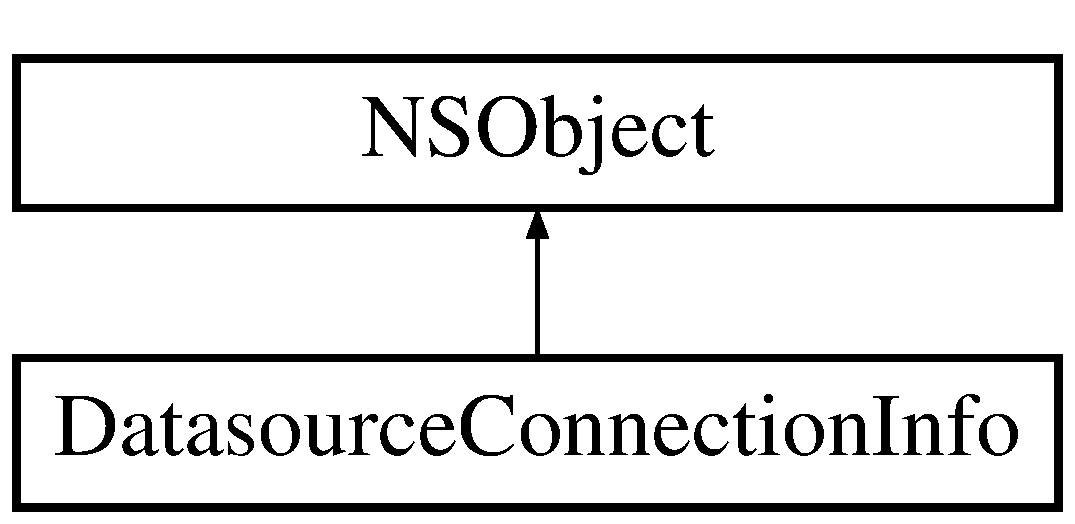
\includegraphics[height=2.000000cm]{interface_datasource_connection_info}
\end{center}
\end{figure}
\subsection*{Instance Methods}
\begin{DoxyCompactItemize}
\item 
(N\-S\-Mutable\-Dictionary $\ast$) -\/ \hyperlink{interface_datasource_connection_info_a0ceff303c12fb308fcdd18f5882d17e0}{to\-N\-S\-Dictionary}
\end{DoxyCompactItemize}
\subsection*{属性}
\begin{DoxyCompactItemize}
\item 
N\-S\-String $\ast$ \hyperlink{interface_datasource_connection_info_a1fd8ccb6acf54c051fa97a331b8e69b6}{alias}
\begin{DoxyCompactList}\small\item\em 数据源别名 \end{DoxyCompactList}\item 
B\-O\-O\-L \hyperlink{interface_datasource_connection_info_ac95c795a9273e09670a35298b89035ae}{connect}
\begin{DoxyCompactList}\small\item\em 数据源是否自动连接数据 \end{DoxyCompactList}\item 
N\-S\-String $\ast$ \hyperlink{interface_datasource_connection_info_a772012bcbe3ad652f6f30deff2d5524c}{data\-Base}
\begin{DoxyCompactList}\small\item\em 数据源连接的数据库名 \end{DoxyCompactList}\item 
N\-S\-String $\ast$ \hyperlink{interface_datasource_connection_info_aff2ec2a3b3bd1f02095f5a33f3b731a6}{driver}
\begin{DoxyCompactList}\small\item\em 使用 O\-D\-B\-C(Open Database Connectivity,开放数据库互连)的数据库的驱动程序名 \end{DoxyCompactList}\item 
B\-O\-O\-L \hyperlink{interface_datasource_connection_info_a15eaa8dfeb1d855e6fec2f9e6ff9820c}{exclusive}
\begin{DoxyCompactList}\small\item\em 是否以独占方式打开数据源 \end{DoxyCompactList}\item 
B\-O\-O\-L \hyperlink{interface_datasource_connection_info_aee6b9e9896d111f150c391a42ff95d16}{Open\-Link\-Table}
\begin{DoxyCompactList}\small\item\em 是否把数据库中的其他非 Super\-Map 数据表作为 Link\-Table 打开 \end{DoxyCompactList}\item 
N\-S\-String $\ast$ \hyperlink{interface_datasource_connection_info_ac2b82870737e9e1e4557e8f8a164b2cd}{password}
\begin{DoxyCompactList}\small\item\em 登录数据源连接的数据库或文件的密码 \end{DoxyCompactList}\item 
B\-O\-O\-L \hyperlink{interface_datasource_connection_info_adc42b6d15d546e28188e6c1bda9963d6}{read\-Only}
\begin{DoxyCompactList}\small\item\em 是否以只读方式打开数据源 \end{DoxyCompactList}\item 
N\-S\-String $\ast$ \hyperlink{interface_datasource_connection_info_a54b5d6573511dc1c6e33dcd409d7824a}{server}
\begin{DoxyCompactList}\small\item\em 数据库服务器名或本地数据文件名 \end{DoxyCompactList}\item 
N\-S\-String $\ast$ \hyperlink{interface_datasource_connection_info_aba83bd0a99c90d5dc6e8f151e5d212f4}{user}
\begin{DoxyCompactList}\small\item\em 登录数据库的用户名 \end{DoxyCompactList}\end{DoxyCompactItemize}


\subsection{详细描述}
数据源连接信息类。 该类包含了数据源名称、数据源连接的数据库或文件等相关信息 

\subsection{Method Documentation}
\hypertarget{interface_datasource_connection_info_a0ceff303c12fb308fcdd18f5882d17e0}{\index{Datasource\-Connection\-Info@{Datasource\-Connection\-Info}!to\-N\-S\-Dictionary@{to\-N\-S\-Dictionary}}
\index{to\-N\-S\-Dictionary@{to\-N\-S\-Dictionary}!DatasourceConnectionInfo@{Datasource\-Connection\-Info}}
\subsubsection[{to\-N\-S\-Dictionary}]{\setlength{\rightskip}{0pt plus 5cm}-\/ (N\-S\-Mutable\-Dictionary $\ast$) to\-N\-S\-Dictionary 
\begin{DoxyParamCaption}
{}
\end{DoxyParamCaption}
}}\label{interface_datasource_connection_info_a0ceff303c12fb308fcdd18f5882d17e0}


\subsection{属性说明}
\hypertarget{interface_datasource_connection_info_a1fd8ccb6acf54c051fa97a331b8e69b6}{\index{Datasource\-Connection\-Info@{Datasource\-Connection\-Info}!alias@{alias}}
\index{alias@{alias}!DatasourceConnectionInfo@{Datasource\-Connection\-Info}}
\subsubsection[{alias}]{\setlength{\rightskip}{0pt plus 5cm}-\/ (N\-S\-String $\ast$) alias\hspace{0.3cm}{\ttfamily [read]}, {\ttfamily [write]}, {\ttfamily [atomic]}, {\ttfamily [copy]}}}\label{interface_datasource_connection_info_a1fd8ccb6acf54c051fa97a331b8e69b6}


数据源别名 

\hypertarget{interface_datasource_connection_info_ac95c795a9273e09670a35298b89035ae}{\index{Datasource\-Connection\-Info@{Datasource\-Connection\-Info}!connect@{connect}}
\index{connect@{connect}!DatasourceConnectionInfo@{Datasource\-Connection\-Info}}
\subsubsection[{connect}]{\setlength{\rightskip}{0pt plus 5cm}-\/ (B\-O\-O\-L) connect\hspace{0.3cm}{\ttfamily [read]}, {\ttfamily [write]}, {\ttfamily [atomic]}, {\ttfamily [assign]}}}\label{interface_datasource_connection_info_ac95c795a9273e09670a35298b89035ae}


数据源是否自动连接数据 

\hypertarget{interface_datasource_connection_info_a772012bcbe3ad652f6f30deff2d5524c}{\index{Datasource\-Connection\-Info@{Datasource\-Connection\-Info}!data\-Base@{data\-Base}}
\index{data\-Base@{data\-Base}!DatasourceConnectionInfo@{Datasource\-Connection\-Info}}
\subsubsection[{data\-Base}]{\setlength{\rightskip}{0pt plus 5cm}-\/ (N\-S\-String $\ast$) data\-Base\hspace{0.3cm}{\ttfamily [read]}, {\ttfamily [write]}, {\ttfamily [atomic]}, {\ttfamily [copy]}}}\label{interface_datasource_connection_info_a772012bcbe3ad652f6f30deff2d5524c}


数据源连接的数据库名 

\hypertarget{interface_datasource_connection_info_aff2ec2a3b3bd1f02095f5a33f3b731a6}{\index{Datasource\-Connection\-Info@{Datasource\-Connection\-Info}!driver@{driver}}
\index{driver@{driver}!DatasourceConnectionInfo@{Datasource\-Connection\-Info}}
\subsubsection[{driver}]{\setlength{\rightskip}{0pt plus 5cm}-\/ (N\-S\-String $\ast$) driver\hspace{0.3cm}{\ttfamily [read]}, {\ttfamily [write]}, {\ttfamily [atomic]}, {\ttfamily [copy]}}}\label{interface_datasource_connection_info_aff2ec2a3b3bd1f02095f5a33f3b731a6}


使用 O\-D\-B\-C(Open Database Connectivity,开放数据库互连)的数据库的驱动程序名 

\hypertarget{interface_datasource_connection_info_a15eaa8dfeb1d855e6fec2f9e6ff9820c}{\index{Datasource\-Connection\-Info@{Datasource\-Connection\-Info}!exclusive@{exclusive}}
\index{exclusive@{exclusive}!DatasourceConnectionInfo@{Datasource\-Connection\-Info}}
\subsubsection[{exclusive}]{\setlength{\rightskip}{0pt plus 5cm}-\/ (B\-O\-O\-L) exclusive\hspace{0.3cm}{\ttfamily [read]}, {\ttfamily [write]}, {\ttfamily [atomic]}, {\ttfamily [assign]}}}\label{interface_datasource_connection_info_a15eaa8dfeb1d855e6fec2f9e6ff9820c}


是否以独占方式打开数据源 

\hypertarget{interface_datasource_connection_info_aee6b9e9896d111f150c391a42ff95d16}{\index{Datasource\-Connection\-Info@{Datasource\-Connection\-Info}!Open\-Link\-Table@{Open\-Link\-Table}}
\index{Open\-Link\-Table@{Open\-Link\-Table}!DatasourceConnectionInfo@{Datasource\-Connection\-Info}}
\subsubsection[{Open\-Link\-Table}]{\setlength{\rightskip}{0pt plus 5cm}-\/ (B\-O\-O\-L) Open\-Link\-Table\hspace{0.3cm}{\ttfamily [read]}, {\ttfamily [write]}, {\ttfamily [atomic]}, {\ttfamily [assign]}}}\label{interface_datasource_connection_info_aee6b9e9896d111f150c391a42ff95d16}


是否把数据库中的其他非 Super\-Map 数据表作为 Link\-Table 打开 

\hypertarget{interface_datasource_connection_info_ac2b82870737e9e1e4557e8f8a164b2cd}{\index{Datasource\-Connection\-Info@{Datasource\-Connection\-Info}!password@{password}}
\index{password@{password}!DatasourceConnectionInfo@{Datasource\-Connection\-Info}}
\subsubsection[{password}]{\setlength{\rightskip}{0pt plus 5cm}-\/ (N\-S\-String $\ast$) password\hspace{0.3cm}{\ttfamily [read]}, {\ttfamily [write]}, {\ttfamily [atomic]}, {\ttfamily [copy]}}}\label{interface_datasource_connection_info_ac2b82870737e9e1e4557e8f8a164b2cd}


登录数据源连接的数据库或文件的密码 

\hypertarget{interface_datasource_connection_info_adc42b6d15d546e28188e6c1bda9963d6}{\index{Datasource\-Connection\-Info@{Datasource\-Connection\-Info}!read\-Only@{read\-Only}}
\index{read\-Only@{read\-Only}!DatasourceConnectionInfo@{Datasource\-Connection\-Info}}
\subsubsection[{read\-Only}]{\setlength{\rightskip}{0pt plus 5cm}-\/ (B\-O\-O\-L) read\-Only\hspace{0.3cm}{\ttfamily [read]}, {\ttfamily [write]}, {\ttfamily [atomic]}, {\ttfamily [assign]}}}\label{interface_datasource_connection_info_adc42b6d15d546e28188e6c1bda9963d6}


是否以只读方式打开数据源 

\hypertarget{interface_datasource_connection_info_a54b5d6573511dc1c6e33dcd409d7824a}{\index{Datasource\-Connection\-Info@{Datasource\-Connection\-Info}!server@{server}}
\index{server@{server}!DatasourceConnectionInfo@{Datasource\-Connection\-Info}}
\subsubsection[{server}]{\setlength{\rightskip}{0pt plus 5cm}-\/ (N\-S\-String $\ast$) server\hspace{0.3cm}{\ttfamily [read]}, {\ttfamily [write]}, {\ttfamily [atomic]}, {\ttfamily [copy]}}}\label{interface_datasource_connection_info_a54b5d6573511dc1c6e33dcd409d7824a}


数据库服务器名或本地数据文件名 

\hypertarget{interface_datasource_connection_info_aba83bd0a99c90d5dc6e8f151e5d212f4}{\index{Datasource\-Connection\-Info@{Datasource\-Connection\-Info}!user@{user}}
\index{user@{user}!DatasourceConnectionInfo@{Datasource\-Connection\-Info}}
\subsubsection[{user}]{\setlength{\rightskip}{0pt plus 5cm}-\/ (N\-S\-String $\ast$) user\hspace{0.3cm}{\ttfamily [read]}, {\ttfamily [write]}, {\ttfamily [atomic]}, {\ttfamily [copy]}}}\label{interface_datasource_connection_info_aba83bd0a99c90d5dc6e8f151e5d212f4}


登录数据库的用户名 



该类的文档由以下文件生成\-:\begin{DoxyCompactItemize}
\item 
Map/\hyperlink{_datasource_connection_info_8h}{Datasource\-Connection\-Info.\-h}\item 
Map/\hyperlink{_datasource_connection_info_8m}{Datasource\-Connection\-Info.\-m}\end{DoxyCompactItemize}

\hypertarget{interface_filter_parameter}{\section{Filter\-Parameter类 参考}
\label{interface_filter_parameter}\index{Filter\-Parameter@{Filter\-Parameter}}
}


查询过滤条件参数类。 \par
 该类用于设置查询数据集的查询过滤参数。  




{\ttfamily \#import $<$Filter\-Parameter.\-h$>$}

类 Filter\-Parameter 继承关系图\-:\begin{figure}[H]
\begin{center}
\leavevmode
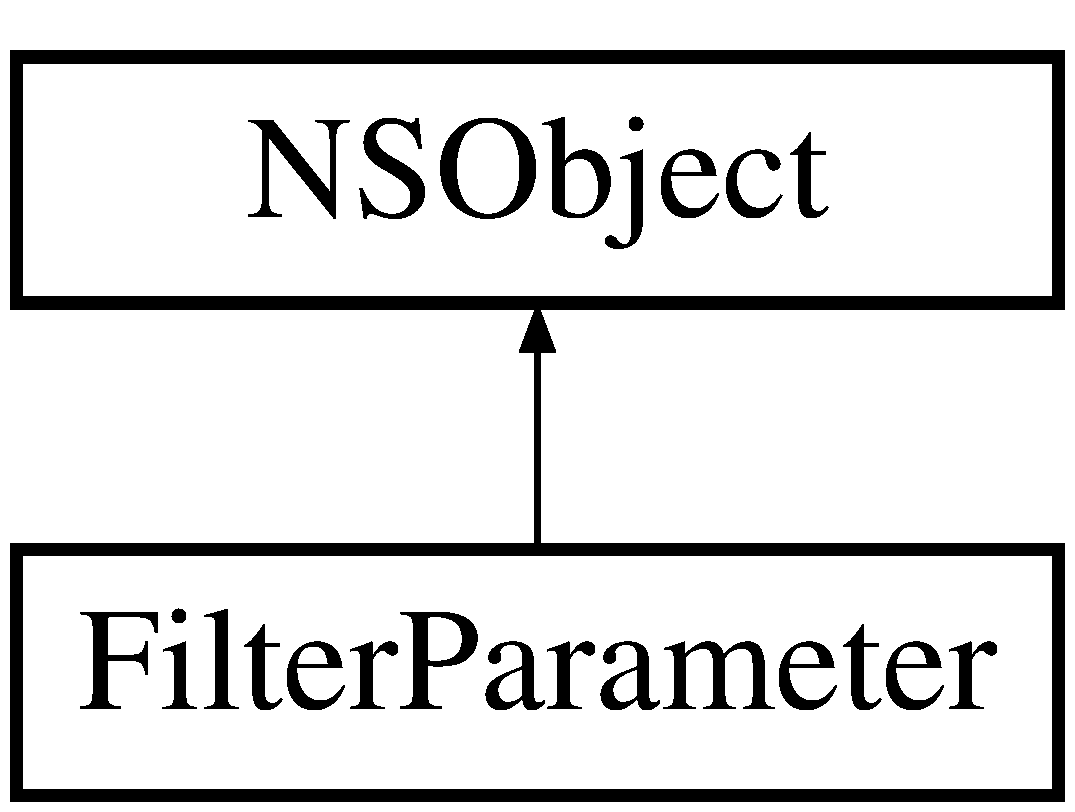
\includegraphics[height=2.000000cm]{interface_filter_parameter}
\end{center}
\end{figure}
\subsection*{Instance Methods}
\begin{DoxyCompactItemize}
\item 
(N\-S\-Mutable\-Dictionary $\ast$) -\/ \hyperlink{interface_filter_parameter_aec58bf3889230a6ab7209ce239fb242e}{to\-N\-S\-Dictionary}
\end{DoxyCompactItemize}
\subsection*{属性}
\begin{DoxyCompactItemize}
\item 
N\-S\-String $\ast$ \hyperlink{interface_filter_parameter_a04bd8e83fd0de6e02737efaf0817821e}{attribute\-Filter}
\item 
N\-S\-Mutable\-Array $\ast$ \hyperlink{interface_filter_parameter_ac4806e37406b21dc3f9e09edd94047b9}{fields}
\item 
N\-S\-String $\ast$ \hyperlink{interface_filter_parameter_a4da1063e06d3211179e35fca8a4043f9}{group\-By}
\item 
N\-S\-Mutable\-Array $\ast$ \hyperlink{interface_filter_parameter_ab6ee6c87b71d464fe5cb5308a2f93977}{ids}
\item 
N\-S\-Mutable\-Array $\ast$ \hyperlink{interface_filter_parameter_a63b04dc5f922c4d6a012933331a76149}{join\-Items}
\item 
N\-S\-Mutable\-Array $\ast$ \hyperlink{interface_filter_parameter_aa6ccb9ad285c9ac4c284a03115a834f5}{link\-Items}
\item 
N\-S\-String $\ast$ \hyperlink{interface_filter_parameter_a32495fe4ce8013104c0433f3467ad743}{name}
\item 
N\-S\-String $\ast$ \hyperlink{interface_filter_parameter_a519e07fe4d3de6fef4514cd20c0eea2b}{order\-By}
\end{DoxyCompactItemize}


\subsection{详细描述}
查询过滤条件参数类。 \par
 该类用于设置查询数据集的查询过滤参数。 

\subsection{Method Documentation}
\hypertarget{interface_filter_parameter_aec58bf3889230a6ab7209ce239fb242e}{\index{Filter\-Parameter@{Filter\-Parameter}!to\-N\-S\-Dictionary@{to\-N\-S\-Dictionary}}
\index{to\-N\-S\-Dictionary@{to\-N\-S\-Dictionary}!FilterParameter@{Filter\-Parameter}}
\subsubsection[{to\-N\-S\-Dictionary}]{\setlength{\rightskip}{0pt plus 5cm}-\/ (N\-S\-Mutable\-Dictionary $\ast$) to\-N\-S\-Dictionary 
\begin{DoxyParamCaption}
{}
\end{DoxyParamCaption}
}}\label{interface_filter_parameter_aec58bf3889230a6ab7209ce239fb242e}


\subsection{属性说明}
\hypertarget{interface_filter_parameter_a04bd8e83fd0de6e02737efaf0817821e}{\index{Filter\-Parameter@{Filter\-Parameter}!attribute\-Filter@{attribute\-Filter}}
\index{attribute\-Filter@{attribute\-Filter}!FilterParameter@{Filter\-Parameter}}
\subsubsection[{attribute\-Filter}]{\setlength{\rightskip}{0pt plus 5cm}-\/ (N\-S\-String $\ast$) attribute\-Filter\hspace{0.3cm}{\ttfamily [read]}, {\ttfamily [write]}, {\ttfamily [atomic]}, {\ttfamily [copy]}}}\label{interface_filter_parameter_a04bd8e83fd0de6e02737efaf0817821e}
\hypertarget{interface_filter_parameter_ac4806e37406b21dc3f9e09edd94047b9}{\index{Filter\-Parameter@{Filter\-Parameter}!fields@{fields}}
\index{fields@{fields}!FilterParameter@{Filter\-Parameter}}
\subsubsection[{fields}]{\setlength{\rightskip}{0pt plus 5cm}-\/ (N\-S\-Mutable\-Array $\ast$) fields\hspace{0.3cm}{\ttfamily [read]}, {\ttfamily [write]}, {\ttfamily [atomic]}, {\ttfamily [retain]}}}\label{interface_filter_parameter_ac4806e37406b21dc3f9e09edd94047b9}
\hypertarget{interface_filter_parameter_a4da1063e06d3211179e35fca8a4043f9}{\index{Filter\-Parameter@{Filter\-Parameter}!group\-By@{group\-By}}
\index{group\-By@{group\-By}!FilterParameter@{Filter\-Parameter}}
\subsubsection[{group\-By}]{\setlength{\rightskip}{0pt plus 5cm}-\/ (N\-S\-String $\ast$) group\-By\hspace{0.3cm}{\ttfamily [read]}, {\ttfamily [write]}, {\ttfamily [atomic]}, {\ttfamily [copy]}}}\label{interface_filter_parameter_a4da1063e06d3211179e35fca8a4043f9}
\hypertarget{interface_filter_parameter_ab6ee6c87b71d464fe5cb5308a2f93977}{\index{Filter\-Parameter@{Filter\-Parameter}!ids@{ids}}
\index{ids@{ids}!FilterParameter@{Filter\-Parameter}}
\subsubsection[{ids}]{\setlength{\rightskip}{0pt plus 5cm}-\/ (N\-S\-Mutable\-Array $\ast$) ids\hspace{0.3cm}{\ttfamily [read]}, {\ttfamily [write]}, {\ttfamily [atomic]}, {\ttfamily [retain]}}}\label{interface_filter_parameter_ab6ee6c87b71d464fe5cb5308a2f93977}
\hypertarget{interface_filter_parameter_a63b04dc5f922c4d6a012933331a76149}{\index{Filter\-Parameter@{Filter\-Parameter}!join\-Items@{join\-Items}}
\index{join\-Items@{join\-Items}!FilterParameter@{Filter\-Parameter}}
\subsubsection[{join\-Items}]{\setlength{\rightskip}{0pt plus 5cm}-\/ (N\-S\-Mutable\-Array $\ast$) join\-Items\hspace{0.3cm}{\ttfamily [read]}, {\ttfamily [write]}, {\ttfamily [atomic]}, {\ttfamily [retain]}}}\label{interface_filter_parameter_a63b04dc5f922c4d6a012933331a76149}


参考自 to\-N\-S\-Dictionary.

\hypertarget{interface_filter_parameter_aa6ccb9ad285c9ac4c284a03115a834f5}{\index{Filter\-Parameter@{Filter\-Parameter}!link\-Items@{link\-Items}}
\index{link\-Items@{link\-Items}!FilterParameter@{Filter\-Parameter}}
\subsubsection[{link\-Items}]{\setlength{\rightskip}{0pt plus 5cm}-\/ (N\-S\-Mutable\-Array $\ast$) link\-Items\hspace{0.3cm}{\ttfamily [read]}, {\ttfamily [write]}, {\ttfamily [atomic]}, {\ttfamily [retain]}}}\label{interface_filter_parameter_aa6ccb9ad285c9ac4c284a03115a834f5}


参考自 to\-N\-S\-Dictionary.

\hypertarget{interface_filter_parameter_a32495fe4ce8013104c0433f3467ad743}{\index{Filter\-Parameter@{Filter\-Parameter}!name@{name}}
\index{name@{name}!FilterParameter@{Filter\-Parameter}}
\subsubsection[{name}]{\setlength{\rightskip}{0pt plus 5cm}-\/ (N\-S\-String $\ast$) name\hspace{0.3cm}{\ttfamily [read]}, {\ttfamily [write]}, {\ttfamily [atomic]}, {\ttfamily [copy]}}}\label{interface_filter_parameter_a32495fe4ce8013104c0433f3467ad743}
\hypertarget{interface_filter_parameter_a519e07fe4d3de6fef4514cd20c0eea2b}{\index{Filter\-Parameter@{Filter\-Parameter}!order\-By@{order\-By}}
\index{order\-By@{order\-By}!FilterParameter@{Filter\-Parameter}}
\subsubsection[{order\-By}]{\setlength{\rightskip}{0pt plus 5cm}-\/ (N\-S\-String $\ast$) order\-By\hspace{0.3cm}{\ttfamily [read]}, {\ttfamily [write]}, {\ttfamily [atomic]}, {\ttfamily [copy]}}}\label{interface_filter_parameter_a519e07fe4d3de6fef4514cd20c0eea2b}


该类的文档由以下文件生成\-:\begin{DoxyCompactItemize}
\item 
Map/\hyperlink{_filter_parameter_8h}{Filter\-Parameter.\-h}\item 
Map/\hyperlink{_filter_parameter_8m}{Filter\-Parameter.\-m}\end{DoxyCompactItemize}

\hypertarget{interface_join_item}{\section{Join\-Item类 参考}
\label{interface_join_item}\index{Join\-Item@{Join\-Item}}
}


连接信息类。\par
 该类用于定义矢量数据集与外部表的连接信息。 外部表可以为另一个矢量数据集(其中纯属性数据集中没有空间几何信息) 所对应的 D\-B\-M\-S(Database Management System,数据库管理系统)表, 也可以是用户自建的业务表。需要注意的是,矢量数据集与外部表必须属于同一数据源。 用于连接两个表的字段的名称不一定相同,但类型必须一致。  




{\ttfamily \#import $<$Join\-Item.\-h$>$}

类 Join\-Item 继承关系图\-:\begin{figure}[H]
\begin{center}
\leavevmode
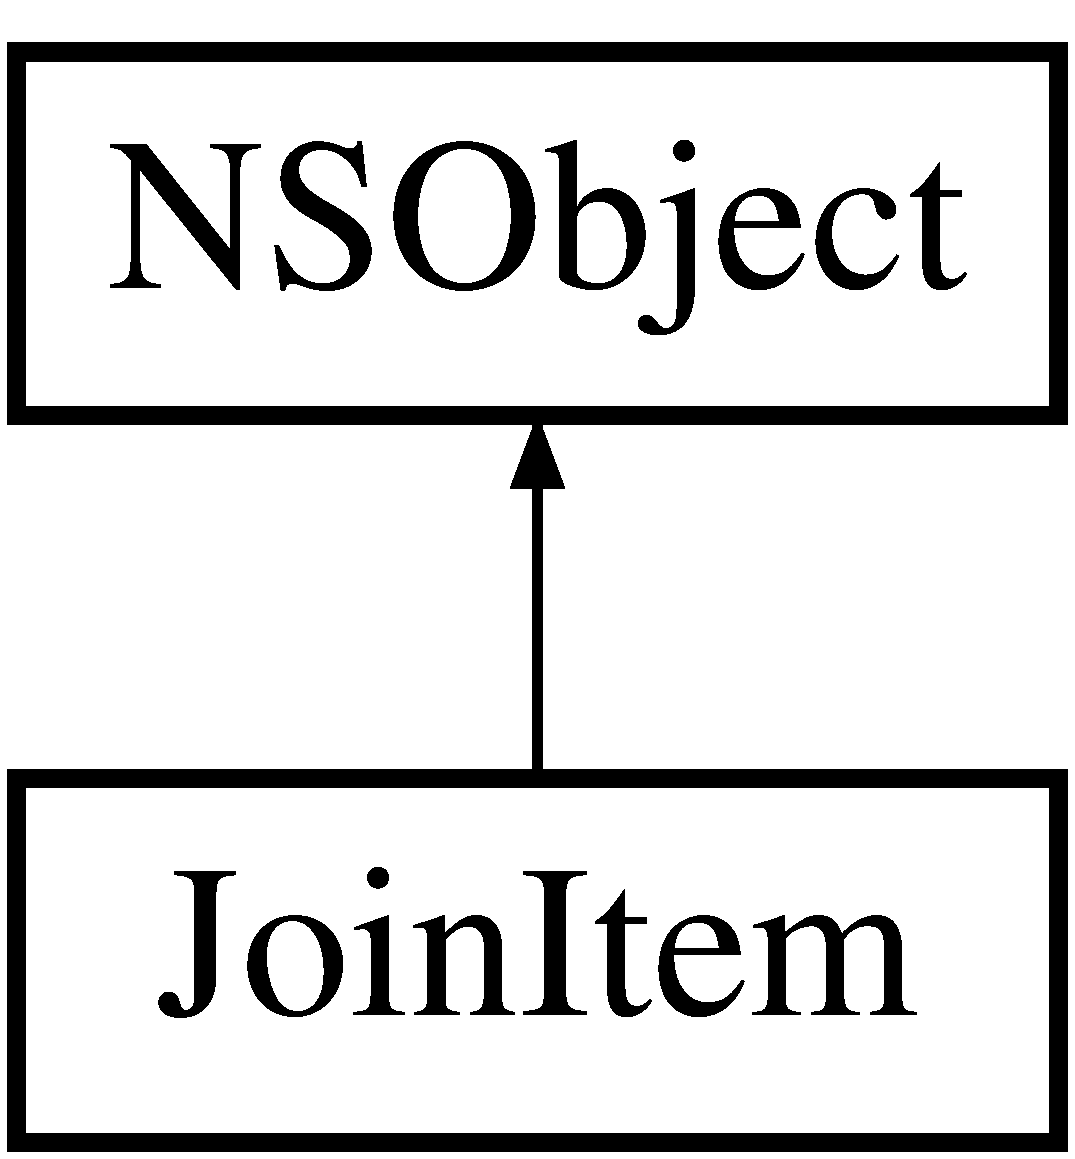
\includegraphics[height=2.000000cm]{interface_join_item}
\end{center}
\end{figure}
\subsection*{Instance Methods}
\begin{DoxyCompactItemize}
\item 
(id) -\/ \hyperlink{interface_join_item_ae6b4f0aecf479050c8cf18170d754554}{init}{\ttfamily  \mbox{[}implementation\mbox{]}}
\item 
(N\-S\-Mutable\-Dictionary $\ast$) -\/ \hyperlink{interface_join_item_a65aa7b6f8fcc79b10406687c599faede}{to\-N\-S\-Dictionary}
\end{DoxyCompactItemize}
\subsection*{属性}
\begin{DoxyCompactItemize}
\item 
N\-S\-String $\ast$ \hyperlink{interface_join_item_a19fdae54d25724191c1f1a253d8283c5}{foreign\-Table\-Name}
\item 
N\-S\-String $\ast$ \hyperlink{interface_join_item_a2dfc110b26f4cf48aeae6cee0c1686ec}{join\-Filter}
\item 
N\-S\-String $\ast$ \hyperlink{interface_join_item_a6aa4f1788a48780bf34a84fa58253057}{join\-Type}
\end{DoxyCompactItemize}


\subsection{详细描述}
连接信息类。\par
 该类用于定义矢量数据集与外部表的连接信息。 外部表可以为另一个矢量数据集(其中纯属性数据集中没有空间几何信息) 所对应的 D\-B\-M\-S(Database Management System,数据库管理系统)表, 也可以是用户自建的业务表。需要注意的是,矢量数据集与外部表必须属于同一数据源。 用于连接两个表的字段的名称不一定相同,但类型必须一致。 

\subsection{Method Documentation}
\hypertarget{interface_join_item_ae6b4f0aecf479050c8cf18170d754554}{\index{Join\-Item@{Join\-Item}!init@{init}}
\index{init@{init}!JoinItem@{Join\-Item}}
\subsubsection[{init}]{\setlength{\rightskip}{0pt plus 5cm}-\/ (id) init 
\begin{DoxyParamCaption}
{}
\end{DoxyParamCaption}
\hspace{0.3cm}{\ttfamily [implementation]}}}\label{interface_join_item_ae6b4f0aecf479050c8cf18170d754554}
\hypertarget{interface_join_item_a65aa7b6f8fcc79b10406687c599faede}{\index{Join\-Item@{Join\-Item}!to\-N\-S\-Dictionary@{to\-N\-S\-Dictionary}}
\index{to\-N\-S\-Dictionary@{to\-N\-S\-Dictionary}!JoinItem@{Join\-Item}}
\subsubsection[{to\-N\-S\-Dictionary}]{\setlength{\rightskip}{0pt plus 5cm}-\/ (N\-S\-Mutable\-Dictionary $\ast$) to\-N\-S\-Dictionary 
\begin{DoxyParamCaption}
{}
\end{DoxyParamCaption}
}}\label{interface_join_item_a65aa7b6f8fcc79b10406687c599faede}


\subsection{属性说明}
\hypertarget{interface_join_item_a19fdae54d25724191c1f1a253d8283c5}{\index{Join\-Item@{Join\-Item}!foreign\-Table\-Name@{foreign\-Table\-Name}}
\index{foreign\-Table\-Name@{foreign\-Table\-Name}!JoinItem@{Join\-Item}}
\subsubsection[{foreign\-Table\-Name}]{\setlength{\rightskip}{0pt plus 5cm}-\/ (N\-S\-String $\ast$) foreign\-Table\-Name\hspace{0.3cm}{\ttfamily [read]}, {\ttfamily [write]}, {\ttfamily [atomic]}, {\ttfamily [copy]}}}\label{interface_join_item_a19fdae54d25724191c1f1a253d8283c5}


参考自 init.

\hypertarget{interface_join_item_a2dfc110b26f4cf48aeae6cee0c1686ec}{\index{Join\-Item@{Join\-Item}!join\-Filter@{join\-Filter}}
\index{join\-Filter@{join\-Filter}!JoinItem@{Join\-Item}}
\subsubsection[{join\-Filter}]{\setlength{\rightskip}{0pt plus 5cm}-\/ (N\-S\-String $\ast$) join\-Filter\hspace{0.3cm}{\ttfamily [read]}, {\ttfamily [write]}, {\ttfamily [atomic]}, {\ttfamily [copy]}}}\label{interface_join_item_a2dfc110b26f4cf48aeae6cee0c1686ec}


参考自 init.

\hypertarget{interface_join_item_a6aa4f1788a48780bf34a84fa58253057}{\index{Join\-Item@{Join\-Item}!join\-Type@{join\-Type}}
\index{join\-Type@{join\-Type}!JoinItem@{Join\-Item}}
\subsubsection[{join\-Type}]{\setlength{\rightskip}{0pt plus 5cm}-\/ (N\-S\-String $\ast$) join\-Type\hspace{0.3cm}{\ttfamily [read]}, {\ttfamily [write]}, {\ttfamily [atomic]}, {\ttfamily [copy]}}}\label{interface_join_item_a6aa4f1788a48780bf34a84fa58253057}


参考自 init.



该类的文档由以下文件生成\-:\begin{DoxyCompactItemize}
\item 
Map/\hyperlink{_join_item_8h}{Join\-Item.\-h}\item 
Map/\hyperlink{_join_item_8m}{Join\-Item.\-m}\end{DoxyCompactItemize}

\hypertarget{interface_link_item}{\section{Link\-Item类 参考}
\label{interface_link_item}\index{Link\-Item@{Link\-Item}}
}


关联信息类。 \par
 该类用于定义矢量数据集与外部表之间的关联信息。 外部表可以为另一个矢量数据集(其中纯属性数据集中没有空间几何信息)所对应的 D\-B\-M\-S 表,也可以是用户自建的业务表。 表之间的联系的建立有两种方式,一种是连接(join),一种是关联(link)。连接的相关设置是通过\-Join\-Item类实现的, 关联的相关设置是通过\-Link\-Item类实现的,另外,用于建立连接的两个表必须在同一个数据源下, 而用于建立关联关系的两个表可以不在同一个数据源下。矢量数据集与外部表可以属于不同的数据源。 使用 \hyperlink{interface_link_item}{Link\-Item} 的约束条件:空间数据和属性数据必须有关联条件,即主空间数据集与外部属性表之间存在关联字段。 主空间数据集:用来与外部表进行关联的数据集。 外部属性表:用户通过 Oracle 或者 S\-Q\-L Server 创建的数据表, 或者是另一个矢量数据集所对应的 D\-B\-M\-S(Database Management System,数据库管理系统)表。  




{\ttfamily \#import $<$Link\-Item.\-h$>$}

类 Link\-Item 继承关系图\-:\begin{figure}[H]
\begin{center}
\leavevmode
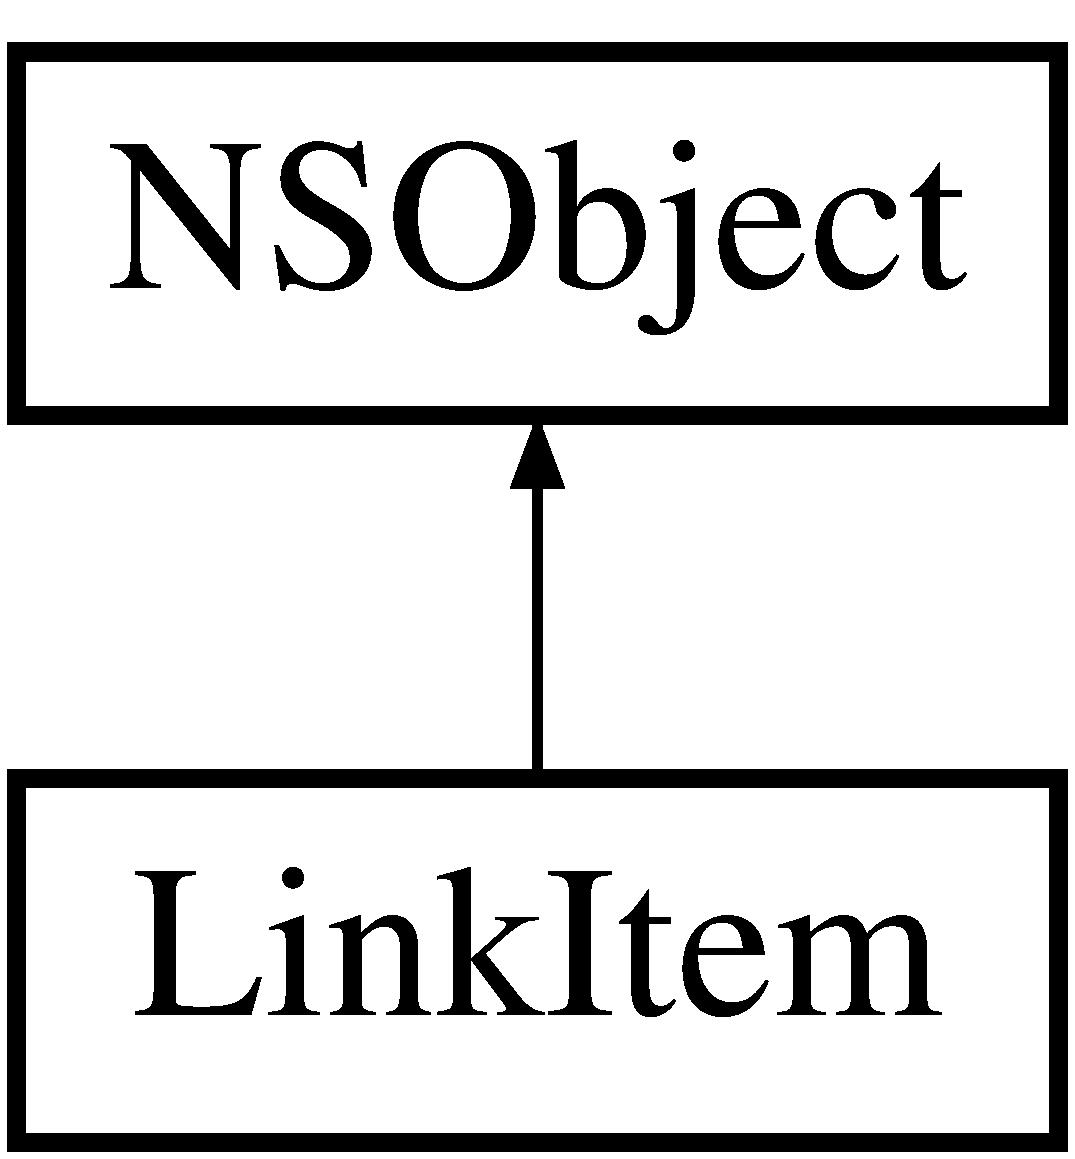
\includegraphics[height=2.000000cm]{interface_link_item}
\end{center}
\end{figure}
\subsection*{Instance Methods}
\begin{DoxyCompactItemize}
\item 
(N\-S\-Mutable\-Dictionary $\ast$) -\/ \hyperlink{interface_link_item_a98a7c06027e61104fb82cacb8558a49d}{to\-N\-S\-Dictionary}
\end{DoxyCompactItemize}
\subsection*{属性}
\begin{DoxyCompactItemize}
\item 
\hyperlink{interface_datasource_connection_info}{Datasource\-Connection\-Info} $\ast$ \hyperlink{interface_link_item_ac227b65db18a97406f2989367279d5b1}{datasource\-Connection\-Info}
\item 
N\-S\-String $\ast$ \hyperlink{interface_link_item_a033a104355e0dd425688c1ace667ee15}{foreign\-Keys}
\item 
N\-S\-String $\ast$ \hyperlink{interface_link_item_a030e9399a97d2a165aa2ce69b798b115}{foreign\-Table}
\item 
N\-S\-String $\ast$ \hyperlink{interface_link_item_a480a48b69d6e2c01fa2bc35f584381f3}{link\-Fields}
\item 
N\-S\-String $\ast$ \hyperlink{interface_link_item_ac1a913e4de4457d2e7fdcc34e7e4d254}{link\-Filter}
\item 
N\-S\-String $\ast$ \hyperlink{interface_link_item_a85d67fda78ae47f1415897d8330f62df}{name}
\item 
N\-S\-Mutable\-Array $\ast$ \hyperlink{interface_link_item_a31d7f4023218fdfef008cec5ae17ea15}{primary\-Keys}
\end{DoxyCompactItemize}


\subsection{详细描述}
关联信息类。 \par
 该类用于定义矢量数据集与外部表之间的关联信息。 外部表可以为另一个矢量数据集(其中纯属性数据集中没有空间几何信息)所对应的 D\-B\-M\-S 表,也可以是用户自建的业务表。 表之间的联系的建立有两种方式,一种是连接(join),一种是关联(link)。连接的相关设置是通过\-Join\-Item类实现的, 关联的相关设置是通过\-Link\-Item类实现的,另外,用于建立连接的两个表必须在同一个数据源下, 而用于建立关联关系的两个表可以不在同一个数据源下。矢量数据集与外部表可以属于不同的数据源。 使用 \hyperlink{interface_link_item}{Link\-Item} 的约束条件:空间数据和属性数据必须有关联条件,即主空间数据集与外部属性表之间存在关联字段。 主空间数据集:用来与外部表进行关联的数据集。 外部属性表:用户通过 Oracle 或者 S\-Q\-L Server 创建的数据表, 或者是另一个矢量数据集所对应的 D\-B\-M\-S(Database Management System,数据库管理系统)表。 

\subsection{Method Documentation}
\hypertarget{interface_link_item_a98a7c06027e61104fb82cacb8558a49d}{\index{Link\-Item@{Link\-Item}!to\-N\-S\-Dictionary@{to\-N\-S\-Dictionary}}
\index{to\-N\-S\-Dictionary@{to\-N\-S\-Dictionary}!LinkItem@{Link\-Item}}
\subsubsection[{to\-N\-S\-Dictionary}]{\setlength{\rightskip}{0pt plus 5cm}-\/ (N\-S\-Mutable\-Dictionary $\ast$) to\-N\-S\-Dictionary 
\begin{DoxyParamCaption}
{}
\end{DoxyParamCaption}
}}\label{interface_link_item_a98a7c06027e61104fb82cacb8558a49d}


\subsection{属性说明}
\hypertarget{interface_link_item_ac227b65db18a97406f2989367279d5b1}{\index{Link\-Item@{Link\-Item}!datasource\-Connection\-Info@{datasource\-Connection\-Info}}
\index{datasource\-Connection\-Info@{datasource\-Connection\-Info}!LinkItem@{Link\-Item}}
\subsubsection[{datasource\-Connection\-Info}]{\setlength{\rightskip}{0pt plus 5cm}-\/ ({\bf Datasource\-Connection\-Info} $\ast$) datasource\-Connection\-Info\hspace{0.3cm}{\ttfamily [read]}, {\ttfamily [write]}, {\ttfamily [atomic]}, {\ttfamily [retain]}}}\label{interface_link_item_ac227b65db18a97406f2989367279d5b1}
\hypertarget{interface_link_item_a033a104355e0dd425688c1ace667ee15}{\index{Link\-Item@{Link\-Item}!foreign\-Keys@{foreign\-Keys}}
\index{foreign\-Keys@{foreign\-Keys}!LinkItem@{Link\-Item}}
\subsubsection[{foreign\-Keys}]{\setlength{\rightskip}{0pt plus 5cm}-\/ (N\-S\-String $\ast$) foreign\-Keys\hspace{0.3cm}{\ttfamily [read]}, {\ttfamily [write]}, {\ttfamily [atomic]}, {\ttfamily [copy]}}}\label{interface_link_item_a033a104355e0dd425688c1ace667ee15}
\hypertarget{interface_link_item_a030e9399a97d2a165aa2ce69b798b115}{\index{Link\-Item@{Link\-Item}!foreign\-Table@{foreign\-Table}}
\index{foreign\-Table@{foreign\-Table}!LinkItem@{Link\-Item}}
\subsubsection[{foreign\-Table}]{\setlength{\rightskip}{0pt plus 5cm}-\/ (N\-S\-String $\ast$) foreign\-Table\hspace{0.3cm}{\ttfamily [read]}, {\ttfamily [write]}, {\ttfamily [atomic]}, {\ttfamily [copy]}}}\label{interface_link_item_a030e9399a97d2a165aa2ce69b798b115}
\hypertarget{interface_link_item_a480a48b69d6e2c01fa2bc35f584381f3}{\index{Link\-Item@{Link\-Item}!link\-Fields@{link\-Fields}}
\index{link\-Fields@{link\-Fields}!LinkItem@{Link\-Item}}
\subsubsection[{link\-Fields}]{\setlength{\rightskip}{0pt plus 5cm}-\/ (N\-S\-String $\ast$) link\-Fields\hspace{0.3cm}{\ttfamily [read]}, {\ttfamily [write]}, {\ttfamily [atomic]}, {\ttfamily [copy]}}}\label{interface_link_item_a480a48b69d6e2c01fa2bc35f584381f3}
\hypertarget{interface_link_item_ac1a913e4de4457d2e7fdcc34e7e4d254}{\index{Link\-Item@{Link\-Item}!link\-Filter@{link\-Filter}}
\index{link\-Filter@{link\-Filter}!LinkItem@{Link\-Item}}
\subsubsection[{link\-Filter}]{\setlength{\rightskip}{0pt plus 5cm}-\/ (N\-S\-String $\ast$) link\-Filter\hspace{0.3cm}{\ttfamily [read]}, {\ttfamily [write]}, {\ttfamily [atomic]}, {\ttfamily [copy]}}}\label{interface_link_item_ac1a913e4de4457d2e7fdcc34e7e4d254}
\hypertarget{interface_link_item_a85d67fda78ae47f1415897d8330f62df}{\index{Link\-Item@{Link\-Item}!name@{name}}
\index{name@{name}!LinkItem@{Link\-Item}}
\subsubsection[{name}]{\setlength{\rightskip}{0pt plus 5cm}-\/ (N\-S\-String $\ast$) name\hspace{0.3cm}{\ttfamily [read]}, {\ttfamily [write]}, {\ttfamily [atomic]}, {\ttfamily [copy]}}}\label{interface_link_item_a85d67fda78ae47f1415897d8330f62df}
\hypertarget{interface_link_item_a31d7f4023218fdfef008cec5ae17ea15}{\index{Link\-Item@{Link\-Item}!primary\-Keys@{primary\-Keys}}
\index{primary\-Keys@{primary\-Keys}!LinkItem@{Link\-Item}}
\subsubsection[{primary\-Keys}]{\setlength{\rightskip}{0pt plus 5cm}-\/ (N\-S\-Mutable\-Array $\ast$) primary\-Keys\hspace{0.3cm}{\ttfamily [read]}, {\ttfamily [write]}, {\ttfamily [atomic]}, {\ttfamily [retain]}}}\label{interface_link_item_a31d7f4023218fdfef008cec5ae17ea15}


该类的文档由以下文件生成\-:\begin{DoxyCompactItemize}
\item 
Map/\hyperlink{_link_item_8h}{Link\-Item.\-h}\item 
Map/\hyperlink{_link_item_8m}{Link\-Item.\-m}\end{DoxyCompactItemize}

\hypertarget{category_n_s_user_defaults_07_route_me_08}{\section{N\-S\-User\-Defaults(Route\-Me)分类 参考}
\label{category_n_s_user_defaults_07_route_me_08}\index{N\-S\-User\-Defaults(\-Route\-Me)@{N\-S\-User\-Defaults(\-Route\-Me)}}
}


{\ttfamily \#import $<$N\-S\-User\-Defaults+\-Route\-Me.\-h$>$}

\subsection*{Instance Methods}
\begin{DoxyCompactItemize}
\item 
(\hyperlink{struct_r_m_projected_point}{R\-M\-Projected\-Point}) -\/ \hyperlink{category_n_s_user_defaults_07_route_me_08_ad8a25763f783a99a2bfadb0da95f8a81}{projected\-Point\-For\-Key\-:}
\begin{DoxyCompactList}\small\item\em Returns the projected point associated with the specified key. \end{DoxyCompactList}\item 
(\hyperlink{struct_r_m_projected_rect}{R\-M\-Projected\-Rect}) -\/ \hyperlink{category_n_s_user_defaults_07_route_me_08_a5030a509dec55919a3c3fe1c1d50742d}{projected\-Rect\-For\-Key\-:}
\begin{DoxyCompactList}\small\item\em Returns the projected rectangle associated with the specified key. \end{DoxyCompactList}\item 
(void) -\/ \hyperlink{category_n_s_user_defaults_07_route_me_08_a52132ca0b7fcca712426d0f206bb9dbf}{set\-Projected\-Point\-:for\-Key\-:}
\begin{DoxyCompactList}\small\item\em Sets the value of the specified default key to the specified projected point. \end{DoxyCompactList}\item 
(void) -\/ \hyperlink{category_n_s_user_defaults_07_route_me_08_a6f6112e9dc8f46e0c9b2bbc004243c8d}{set\-Projected\-Rect\-:for\-Key\-:}
\begin{DoxyCompactList}\small\item\em Sets the value of the specified default key to the specified projected rectangle. \end{DoxyCompactList}\end{DoxyCompactItemize}


\subsection{Method Documentation}
\hypertarget{category_n_s_user_defaults_07_route_me_08_ad8a25763f783a99a2bfadb0da95f8a81}{\index{N\-S\-User\-Defaults(\-Route\-Me)@{N\-S\-User\-Defaults(\-Route\-Me)}!projected\-Point\-For\-Key\-:@{projected\-Point\-For\-Key\-:}}
\index{projected\-Point\-For\-Key\-:@{projected\-Point\-For\-Key\-:}!NSUserDefaults(RouteMe)@{N\-S\-User\-Defaults(\-Route\-Me)}}
\subsubsection[{projected\-Point\-For\-Key\-:}]{\setlength{\rightskip}{0pt plus 5cm}-\/ ({\bf R\-M\-Projected\-Point}) projected\-Point\-For\-Key\-: 
\begin{DoxyParamCaption}
\item[{(N\-S\-String $\ast$)}]{key}
\end{DoxyParamCaption}
}}\label{category_n_s_user_defaults_07_route_me_08_ad8a25763f783a99a2bfadb0da95f8a81}


Returns the projected point associated with the specified key. 

\hypertarget{category_n_s_user_defaults_07_route_me_08_a5030a509dec55919a3c3fe1c1d50742d}{\index{N\-S\-User\-Defaults(\-Route\-Me)@{N\-S\-User\-Defaults(\-Route\-Me)}!projected\-Rect\-For\-Key\-:@{projected\-Rect\-For\-Key\-:}}
\index{projected\-Rect\-For\-Key\-:@{projected\-Rect\-For\-Key\-:}!NSUserDefaults(RouteMe)@{N\-S\-User\-Defaults(\-Route\-Me)}}
\subsubsection[{projected\-Rect\-For\-Key\-:}]{\setlength{\rightskip}{0pt plus 5cm}-\/ ({\bf R\-M\-Projected\-Rect}) projected\-Rect\-For\-Key\-: 
\begin{DoxyParamCaption}
\item[{(N\-S\-String $\ast$)}]{key}
\end{DoxyParamCaption}
}}\label{category_n_s_user_defaults_07_route_me_08_a5030a509dec55919a3c3fe1c1d50742d}


Returns the projected rectangle associated with the specified key. 

\hypertarget{category_n_s_user_defaults_07_route_me_08_a52132ca0b7fcca712426d0f206bb9dbf}{\index{N\-S\-User\-Defaults(\-Route\-Me)@{N\-S\-User\-Defaults(\-Route\-Me)}!set\-Projected\-Point\-:for\-Key\-:@{set\-Projected\-Point\-:for\-Key\-:}}
\index{set\-Projected\-Point\-:for\-Key\-:@{set\-Projected\-Point\-:for\-Key\-:}!NSUserDefaults(RouteMe)@{N\-S\-User\-Defaults(\-Route\-Me)}}
\subsubsection[{set\-Projected\-Point\-:for\-Key\-:}]{\setlength{\rightskip}{0pt plus 5cm}-\/ (void) set\-Projected\-Point\-: 
\begin{DoxyParamCaption}
\item[{({\bf R\-M\-Projected\-Point})}]{projected\-Point}
\item[{forKey:(N\-S\-String $\ast$)}]{key}
\end{DoxyParamCaption}
}}\label{category_n_s_user_defaults_07_route_me_08_a52132ca0b7fcca712426d0f206bb9dbf}


Sets the value of the specified default key to the specified projected point. 

\hypertarget{category_n_s_user_defaults_07_route_me_08_a6f6112e9dc8f46e0c9b2bbc004243c8d}{\index{N\-S\-User\-Defaults(\-Route\-Me)@{N\-S\-User\-Defaults(\-Route\-Me)}!set\-Projected\-Rect\-:for\-Key\-:@{set\-Projected\-Rect\-:for\-Key\-:}}
\index{set\-Projected\-Rect\-:for\-Key\-:@{set\-Projected\-Rect\-:for\-Key\-:}!NSUserDefaults(RouteMe)@{N\-S\-User\-Defaults(\-Route\-Me)}}
\subsubsection[{set\-Projected\-Rect\-:for\-Key\-:}]{\setlength{\rightskip}{0pt plus 5cm}-\/ (void) set\-Projected\-Rect\-: 
\begin{DoxyParamCaption}
\item[{({\bf R\-M\-Projected\-Rect})}]{projected\-Rect}
\item[{forKey:(N\-S\-String $\ast$)}]{key}
\end{DoxyParamCaption}
}}\label{category_n_s_user_defaults_07_route_me_08_a6f6112e9dc8f46e0c9b2bbc004243c8d}


Sets the value of the specified default key to the specified projected rectangle. 



该分类的文档由以下文件生成\-:\begin{DoxyCompactItemize}
\item 
Map/\hyperlink{_n_s_user_defaults_09_route_me_8h}{N\-S\-User\-Defaults+\-Route\-Me.\-h}\item 
Map/\hyperlink{_n_s_user_defaults_09_route_me_8m}{N\-S\-User\-Defaults+\-Route\-Me.\-m}\end{DoxyCompactItemize}

\hypertarget{interface_query_by_bounds_parameters}{\section{Query\-By\-Bounds\-Parameters类 参考}
\label{interface_query_by_bounds_parameters}\index{Query\-By\-Bounds\-Parameters@{Query\-By\-Bounds\-Parameters}}
}


Bounds 查询参数类。\par
 该类用于设置 Bounds 查询的相关参数。  




{\ttfamily \#import $<$Query\-By\-Bounds\-Parameters.\-h$>$}

类 Query\-By\-Bounds\-Parameters 继承关系图\-:\begin{figure}[H]
\begin{center}
\leavevmode
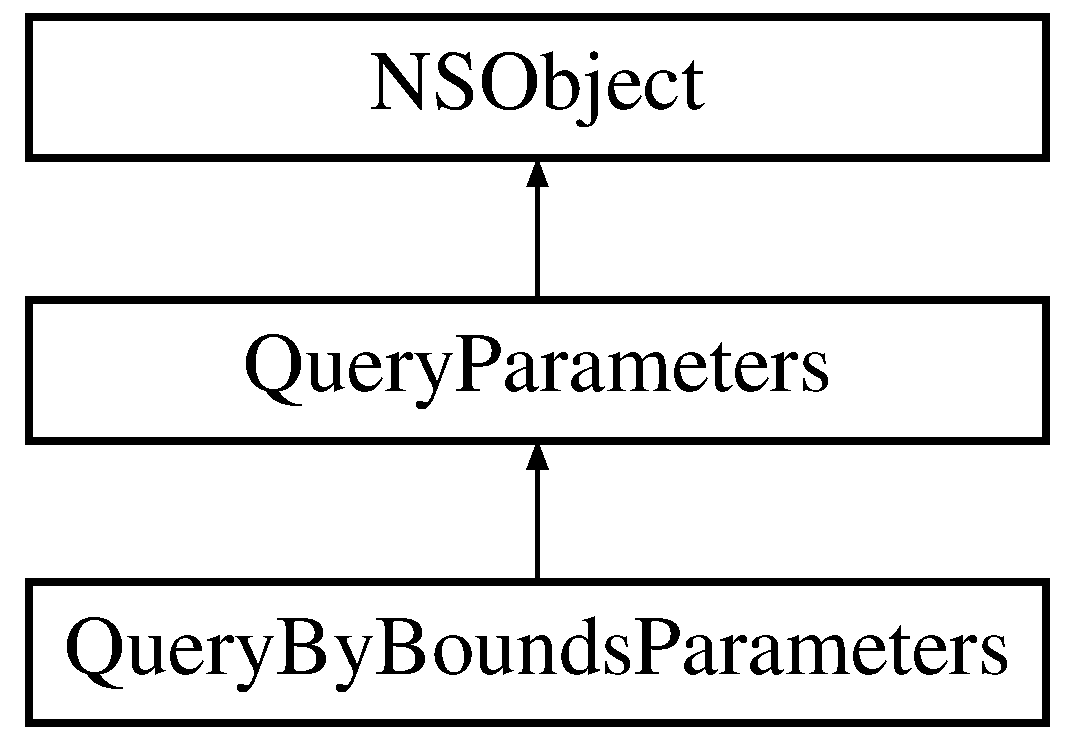
\includegraphics[height=3.000000cm]{interface_query_by_bounds_parameters}
\end{center}
\end{figure}
\subsection*{Instance Methods}
\begin{DoxyCompactItemize}
\item 
(id) -\/ \hyperlink{interface_query_by_bounds_parameters_acb773dfd68fb97595231ccc4eddc90f3}{init\-:}
\end{DoxyCompactItemize}
\subsection*{属性}
\begin{DoxyCompactItemize}
\item 
\hyperlink{struct_r_m_projected_rect}{R\-M\-Projected\-Rect} \hyperlink{interface_query_by_bounds_parameters_ad2e99aa8692b438342762ff18a867b6e}{bounds}
\end{DoxyCompactItemize}


\subsection{详细描述}
Bounds 查询参数类。\par
 该类用于设置 Bounds 查询的相关参数。 

\subsection{Method Documentation}
\hypertarget{interface_query_by_bounds_parameters_acb773dfd68fb97595231ccc4eddc90f3}{\index{Query\-By\-Bounds\-Parameters@{Query\-By\-Bounds\-Parameters}!init\-:@{init\-:}}
\index{init\-:@{init\-:}!QueryByBoundsParameters@{Query\-By\-Bounds\-Parameters}}
\subsubsection[{init\-:}]{\setlength{\rightskip}{0pt plus 5cm}-\/ (id) init\-: 
\begin{DoxyParamCaption}
\item[{({\bf R\-M\-Projected\-Rect})}]{mbounds}
\end{DoxyParamCaption}
}}\label{interface_query_by_bounds_parameters_acb773dfd68fb97595231ccc4eddc90f3}


\subsection{属性说明}
\hypertarget{interface_query_by_bounds_parameters_ad2e99aa8692b438342762ff18a867b6e}{\index{Query\-By\-Bounds\-Parameters@{Query\-By\-Bounds\-Parameters}!bounds@{bounds}}
\index{bounds@{bounds}!QueryByBoundsParameters@{Query\-By\-Bounds\-Parameters}}
\subsubsection[{bounds}]{\setlength{\rightskip}{0pt plus 5cm}-\/ ({\bf R\-M\-Projected\-Rect}) bounds\hspace{0.3cm}{\ttfamily [read]}, {\ttfamily [write]}, {\ttfamily [atomic]}, {\ttfamily [assign]}}}\label{interface_query_by_bounds_parameters_ad2e99aa8692b438342762ff18a867b6e}


参考自 Query\-By\-Bounds\-Service\-::get\-Json\-Parameters\-: , 以及 init\-:.



该类的文档由以下文件生成\-:\begin{DoxyCompactItemize}
\item 
Map/\hyperlink{_query_by_bounds_parameters_8h}{Query\-By\-Bounds\-Parameters.\-h}\item 
Map/\hyperlink{_query_by_bounds_parameters_8m}{Query\-By\-Bounds\-Parameters.\-m}\end{DoxyCompactItemize}

\hypertarget{interface_query_by_bounds_service}{\section{Query\-By\-Bounds\-Service类 参考}
\label{interface_query_by_bounds_service}\index{Query\-By\-Bounds\-Service@{Query\-By\-Bounds\-Service}}
}


Bounds 查询服务类。  




{\ttfamily \#import $<$Query\-By\-Bounds\-Service.\-h$>$}

类 Query\-By\-Bounds\-Service 继承关系图\-:\begin{figure}[H]
\begin{center}
\leavevmode
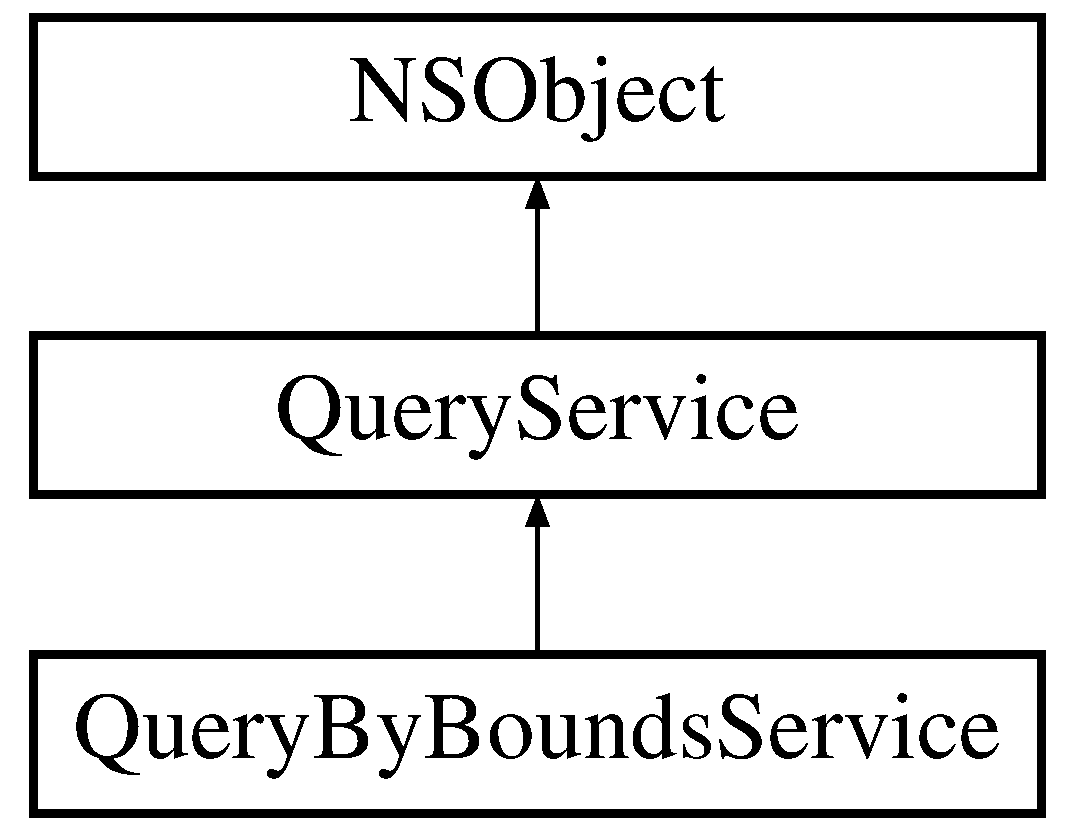
\includegraphics[height=3.000000cm]{interface_query_by_bounds_service}
\end{center}
\end{figure}
\subsection*{Instance Methods}
\begin{DoxyCompactItemize}
\item 
(N\-S\-String $\ast$) -\/ \hyperlink{interface_query_by_bounds_service_ac4d5fe31a786019c71601e95f5d89b8b}{get\-Json\-Parameters\-:}
\item 
(id) -\/ \hyperlink{interface_query_by_bounds_service_afcfdeda43709e2e71d09724a00e6a8cc}{init}
\end{DoxyCompactItemize}
\subsection*{额外继承的成员函数}


\subsection{详细描述}
Bounds 查询服务类。 

\subsection{Method Documentation}
\hypertarget{interface_query_by_bounds_service_ac4d5fe31a786019c71601e95f5d89b8b}{\index{Query\-By\-Bounds\-Service@{Query\-By\-Bounds\-Service}!get\-Json\-Parameters\-:@{get\-Json\-Parameters\-:}}
\index{get\-Json\-Parameters\-:@{get\-Json\-Parameters\-:}!QueryByBoundsService@{Query\-By\-Bounds\-Service}}
\subsubsection[{get\-Json\-Parameters\-:}]{\setlength{\rightskip}{0pt plus 5cm}-\/ (N\-S\-String $\ast$) get\-Json\-Parameters\-: 
\begin{DoxyParamCaption}
\item[{({\bf Query\-Parameters}$\ast$)}]{params}
\end{DoxyParamCaption}
}}\label{interface_query_by_bounds_service_ac4d5fe31a786019c71601e95f5d89b8b}
\hypertarget{interface_query_by_bounds_service_afcfdeda43709e2e71d09724a00e6a8cc}{\index{Query\-By\-Bounds\-Service@{Query\-By\-Bounds\-Service}!init@{init}}
\index{init@{init}!QueryByBoundsService@{Query\-By\-Bounds\-Service}}
\subsubsection[{init}]{\setlength{\rightskip}{0pt plus 5cm}-\/ (id) init 
\begin{DoxyParamCaption}
{}
\end{DoxyParamCaption}
}}\label{interface_query_by_bounds_service_afcfdeda43709e2e71d09724a00e6a8cc}


该类的文档由以下文件生成\-:\begin{DoxyCompactItemize}
\item 
Map/\hyperlink{_query_by_bounds_service_8h}{Query\-By\-Bounds\-Service.\-h}\item 
Map/\hyperlink{_query_by_bounds_service_8m}{Query\-By\-Bounds\-Service.\-m}\end{DoxyCompactItemize}

\hypertarget{interface_query_by_distance_parameters}{\section{Query\-By\-Distance\-Parameters类 参考}
\label{interface_query_by_distance_parameters}\index{Query\-By\-Distance\-Parameters@{Query\-By\-Distance\-Parameters}}
}


Distance 查询参数类。\par
 该类用于设置 Distance 查询的相关参数。  




{\ttfamily \#import $<$Query\-By\-Distance\-Parameters.\-h$>$}

类 Query\-By\-Distance\-Parameters 继承关系图\-:\begin{figure}[H]
\begin{center}
\leavevmode
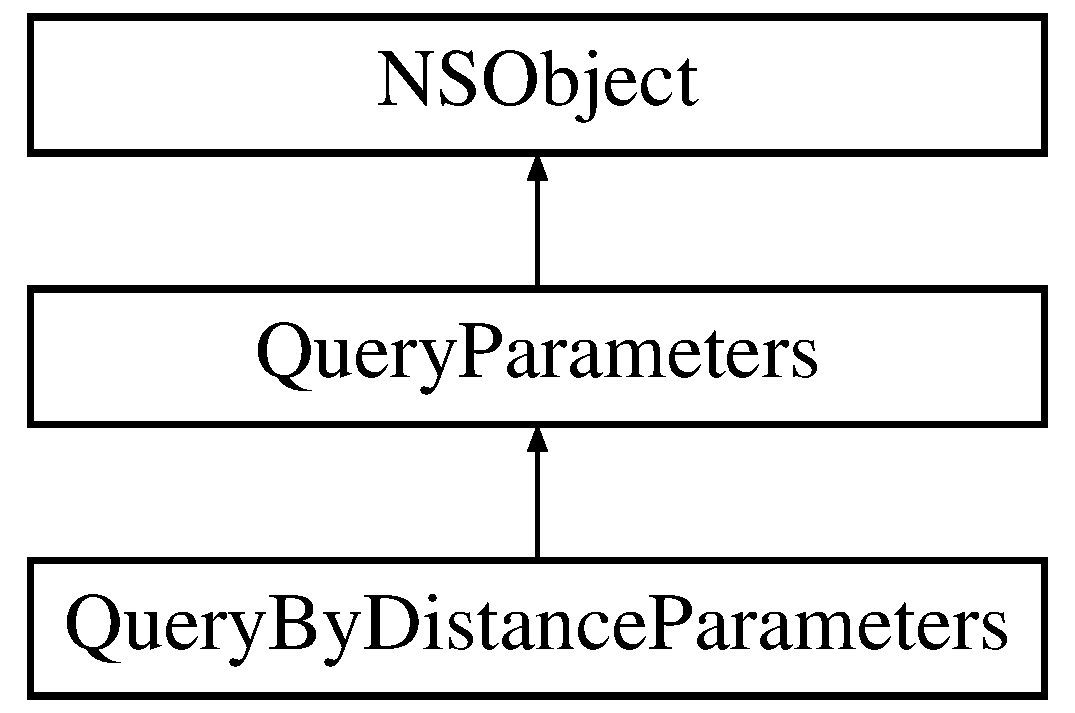
\includegraphics[height=3.000000cm]{interface_query_by_distance_parameters}
\end{center}
\end{figure}
\subsection*{Instance Methods}
\begin{DoxyCompactItemize}
\item 
(id) -\/ \hyperlink{interface_query_by_distance_parameters_ae53a8d12fd2fca675c20d8992de5904d}{init\-:m\-Geometry\-:b\-Nearest\-:}
\end{DoxyCompactItemize}
\subsection*{属性}
\begin{DoxyCompactItemize}
\item 
int \hyperlink{interface_query_by_distance_parameters_ac1c0a5fa9f00deef5914f67e1f95df54}{distance}
\item 
\hyperlink{interface_r_m_path}{R\-M\-Path} $\ast$ \hyperlink{interface_query_by_distance_parameters_a4eeba7af45b232d8a0354f13e4e033b4}{geometry}
\item 
B\-O\-O\-L \hyperlink{interface_query_by_distance_parameters_a45bb2b68e940f017d2809a6ba9485a89}{is\-Nearest}
\end{DoxyCompactItemize}


\subsection{详细描述}
Distance 查询参数类。\par
 该类用于设置 Distance 查询的相关参数。 

\subsection{Method Documentation}
\hypertarget{interface_query_by_distance_parameters_ae53a8d12fd2fca675c20d8992de5904d}{\index{Query\-By\-Distance\-Parameters@{Query\-By\-Distance\-Parameters}!init\-:m\-Geometry\-:b\-Nearest\-:@{init\-:m\-Geometry\-:b\-Nearest\-:}}
\index{init\-:m\-Geometry\-:b\-Nearest\-:@{init\-:m\-Geometry\-:b\-Nearest\-:}!QueryByDistanceParameters@{Query\-By\-Distance\-Parameters}}
\subsubsection[{init\-:m\-Geometry\-:b\-Nearest\-:}]{\setlength{\rightskip}{0pt plus 5cm}-\/ (id) init\-: 
\begin{DoxyParamCaption}
\item[{(int)}]{dis}
\item[{mGeometry:({\bf R\-M\-Path}$\ast$)}]{m\-Geometry}
\item[{bNearest:(B\-O\-O\-L)}]{b\-Nearest}
\end{DoxyParamCaption}
}}\label{interface_query_by_distance_parameters_ae53a8d12fd2fca675c20d8992de5904d}


\subsection{属性说明}
\hypertarget{interface_query_by_distance_parameters_ac1c0a5fa9f00deef5914f67e1f95df54}{\index{Query\-By\-Distance\-Parameters@{Query\-By\-Distance\-Parameters}!distance@{distance}}
\index{distance@{distance}!QueryByDistanceParameters@{Query\-By\-Distance\-Parameters}}
\subsubsection[{distance}]{\setlength{\rightskip}{0pt plus 5cm}-\/ (int) distance\hspace{0.3cm}{\ttfamily [read]}, {\ttfamily [write]}, {\ttfamily [atomic]}, {\ttfamily [assign]}}}\label{interface_query_by_distance_parameters_ac1c0a5fa9f00deef5914f67e1f95df54}


参考自 init\-:m\-Geometry\-:b\-Nearest\-:.

\hypertarget{interface_query_by_distance_parameters_a4eeba7af45b232d8a0354f13e4e033b4}{\index{Query\-By\-Distance\-Parameters@{Query\-By\-Distance\-Parameters}!geometry@{geometry}}
\index{geometry@{geometry}!QueryByDistanceParameters@{Query\-By\-Distance\-Parameters}}
\subsubsection[{geometry}]{\setlength{\rightskip}{0pt plus 5cm}-\/ ({\bf R\-M\-Path} $\ast$) geometry\hspace{0.3cm}{\ttfamily [read]}, {\ttfamily [write]}, {\ttfamily [atomic]}, {\ttfamily [copy]}}}\label{interface_query_by_distance_parameters_a4eeba7af45b232d8a0354f13e4e033b4}


参考自 init\-:m\-Geometry\-:b\-Nearest\-:.

\hypertarget{interface_query_by_distance_parameters_a45bb2b68e940f017d2809a6ba9485a89}{\index{Query\-By\-Distance\-Parameters@{Query\-By\-Distance\-Parameters}!is\-Nearest@{is\-Nearest}}
\index{is\-Nearest@{is\-Nearest}!QueryByDistanceParameters@{Query\-By\-Distance\-Parameters}}
\subsubsection[{is\-Nearest}]{\setlength{\rightskip}{0pt plus 5cm}-\/ (B\-O\-O\-L) is\-Nearest\hspace{0.3cm}{\ttfamily [read]}, {\ttfamily [write]}, {\ttfamily [atomic]}, {\ttfamily [assign]}}}\label{interface_query_by_distance_parameters_a45bb2b68e940f017d2809a6ba9485a89}


参考自 init\-:m\-Geometry\-:b\-Nearest\-:.



该类的文档由以下文件生成\-:\begin{DoxyCompactItemize}
\item 
Map/\hyperlink{_query_by_distance_parameters_8h}{Query\-By\-Distance\-Parameters.\-h}\item 
Map/\hyperlink{_query_by_distance_parameters_8m}{Query\-By\-Distance\-Parameters.\-m}\end{DoxyCompactItemize}

\hypertarget{interface_query_by_distance_service}{\section{Query\-By\-Distance\-Service类 参考}
\label{interface_query_by_distance_service}\index{Query\-By\-Distance\-Service@{Query\-By\-Distance\-Service}}
}


Distance查询服务类。  




{\ttfamily \#import $<$Query\-By\-Distance\-Service.\-h$>$}

类 Query\-By\-Distance\-Service 继承关系图\-:\begin{figure}[H]
\begin{center}
\leavevmode
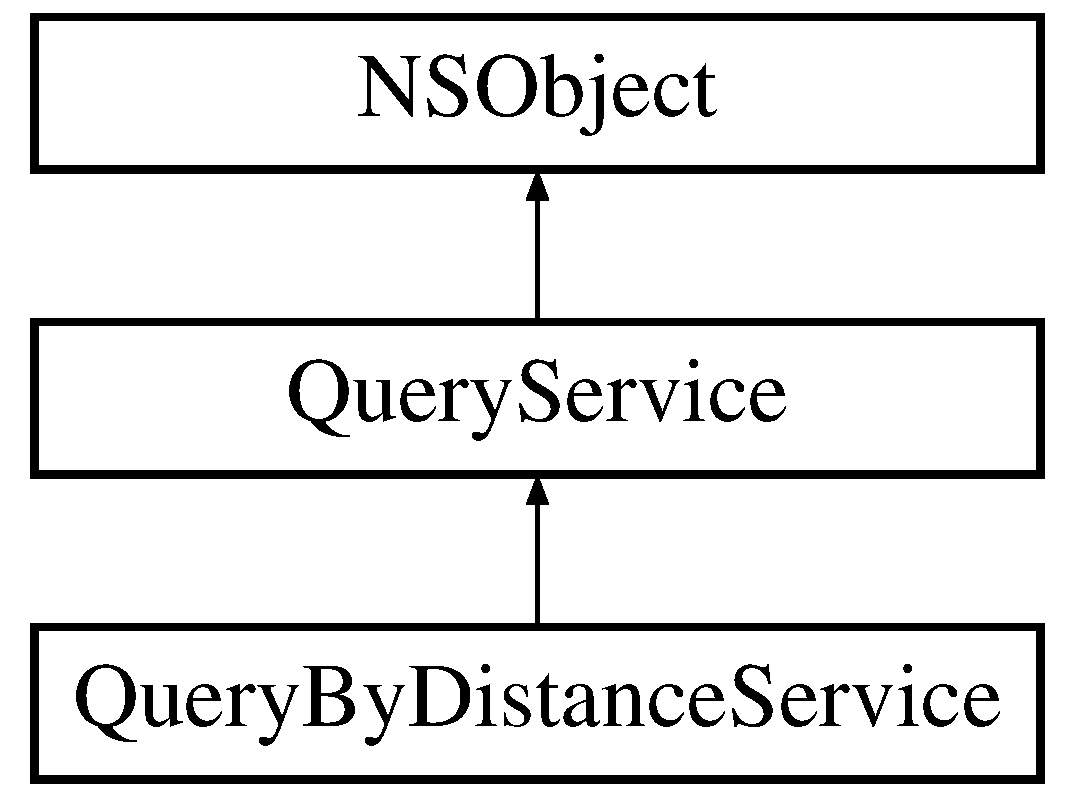
\includegraphics[height=3.000000cm]{interface_query_by_distance_service}
\end{center}
\end{figure}
\subsection*{Instance Methods}
\begin{DoxyCompactItemize}
\item 
(N\-S\-String $\ast$) -\/ \hyperlink{interface_query_by_distance_service_af4ca093849e99a0eba9c78f5ea1f0ae5}{get\-Json\-Parameters\-:}
\item 
(id) -\/ \hyperlink{interface_query_by_distance_service_a2ffafeb5945e78ba50d4a9276d453948}{init}
\end{DoxyCompactItemize}
\subsection*{额外继承的成员函数}


\subsection{详细描述}
Distance查询服务类。 

\subsection{Method Documentation}
\hypertarget{interface_query_by_distance_service_af4ca093849e99a0eba9c78f5ea1f0ae5}{\index{Query\-By\-Distance\-Service@{Query\-By\-Distance\-Service}!get\-Json\-Parameters\-:@{get\-Json\-Parameters\-:}}
\index{get\-Json\-Parameters\-:@{get\-Json\-Parameters\-:}!QueryByDistanceService@{Query\-By\-Distance\-Service}}
\subsubsection[{get\-Json\-Parameters\-:}]{\setlength{\rightskip}{0pt plus 5cm}-\/ (N\-S\-String $\ast$) get\-Json\-Parameters\-: 
\begin{DoxyParamCaption}
\item[{({\bf Query\-Parameters}$\ast$)}]{params}
\end{DoxyParamCaption}
}}\label{interface_query_by_distance_service_af4ca093849e99a0eba9c78f5ea1f0ae5}
\hypertarget{interface_query_by_distance_service_a2ffafeb5945e78ba50d4a9276d453948}{\index{Query\-By\-Distance\-Service@{Query\-By\-Distance\-Service}!init@{init}}
\index{init@{init}!QueryByDistanceService@{Query\-By\-Distance\-Service}}
\subsubsection[{init}]{\setlength{\rightskip}{0pt plus 5cm}-\/ (id) init 
\begin{DoxyParamCaption}
{}
\end{DoxyParamCaption}
}}\label{interface_query_by_distance_service_a2ffafeb5945e78ba50d4a9276d453948}


该类的文档由以下文件生成\-:\begin{DoxyCompactItemize}
\item 
Map/\hyperlink{_query_by_distance_service_8h}{Query\-By\-Distance\-Service.\-h}\item 
Map/\hyperlink{_query_by_distance_service_8m}{Query\-By\-Distance\-Service.\-m}\end{DoxyCompactItemize}

\hypertarget{interface_query_by_geometry_parameters}{\section{Query\-By\-Geometry\-Parameters类 参考}
\label{interface_query_by_geometry_parameters}\index{Query\-By\-Geometry\-Parameters@{Query\-By\-Geometry\-Parameters}}
}


Geometry 查询参数类。 该类用于设置 Geometry查询的相关参数。  




{\ttfamily \#import $<$Query\-By\-Geometry\-Parameters.\-h$>$}

类 Query\-By\-Geometry\-Parameters 继承关系图\-:\begin{figure}[H]
\begin{center}
\leavevmode
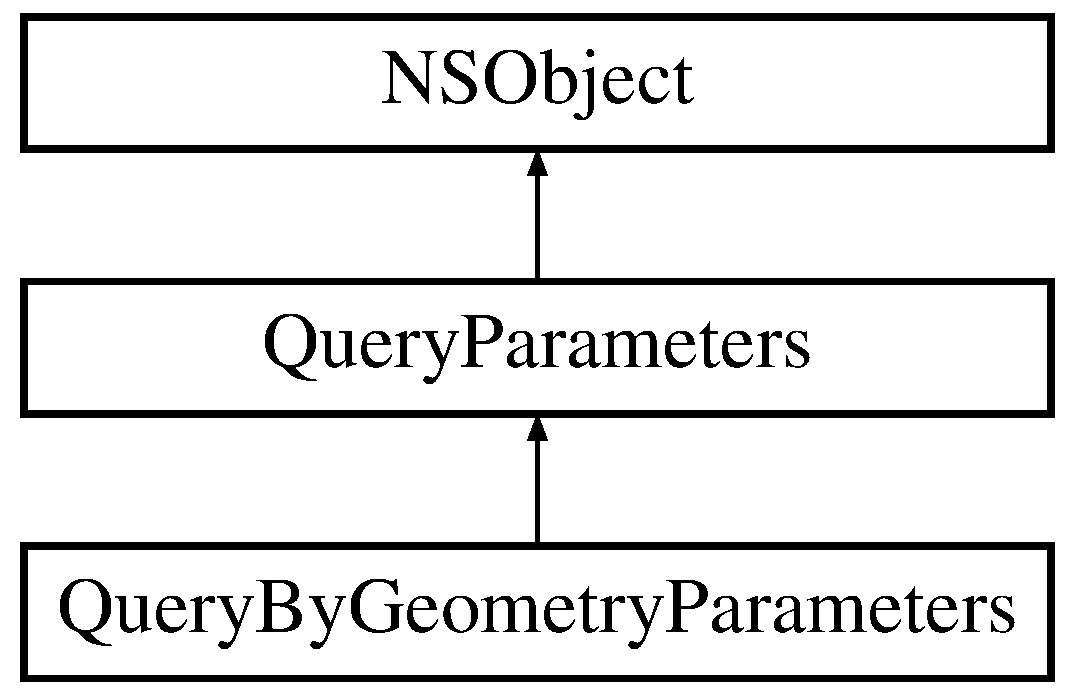
\includegraphics[height=3.000000cm]{interface_query_by_geometry_parameters}
\end{center}
\end{figure}
\subsection*{Instance Methods}
\begin{DoxyCompactItemize}
\item 
(id) -\/ \hyperlink{interface_query_by_geometry_parameters_a1af5a7b4aa2971a828d92bb034264b8e}{init\-:}
\end{DoxyCompactItemize}
\subsection*{属性}
\begin{DoxyCompactItemize}
\item 
\hyperlink{interface_r_m_path}{R\-M\-Path} $\ast$ \hyperlink{interface_query_by_geometry_parameters_ac10c0247460c6c4b3cb67db86958d376}{geometry}
\item 
N\-S\-String $\ast$ \hyperlink{interface_query_by_geometry_parameters_a8487decf8e4c51304266676f62cd83fa}{spatial\-Query\-Mode}
\end{DoxyCompactItemize}


\subsection{详细描述}
Geometry 查询参数类。 该类用于设置 Geometry查询的相关参数。 

\subsection{Method Documentation}
\hypertarget{interface_query_by_geometry_parameters_a1af5a7b4aa2971a828d92bb034264b8e}{\index{Query\-By\-Geometry\-Parameters@{Query\-By\-Geometry\-Parameters}!init\-:@{init\-:}}
\index{init\-:@{init\-:}!QueryByGeometryParameters@{Query\-By\-Geometry\-Parameters}}
\subsubsection[{init\-:}]{\setlength{\rightskip}{0pt plus 5cm}-\/ (id) init\-: 
\begin{DoxyParamCaption}
\item[{({\bf R\-M\-Path}$\ast$)}]{m\-Geo}
\end{DoxyParamCaption}
}}\label{interface_query_by_geometry_parameters_a1af5a7b4aa2971a828d92bb034264b8e}


\subsection{属性说明}
\hypertarget{interface_query_by_geometry_parameters_ac10c0247460c6c4b3cb67db86958d376}{\index{Query\-By\-Geometry\-Parameters@{Query\-By\-Geometry\-Parameters}!geometry@{geometry}}
\index{geometry@{geometry}!QueryByGeometryParameters@{Query\-By\-Geometry\-Parameters}}
\subsubsection[{geometry}]{\setlength{\rightskip}{0pt plus 5cm}-\/ ({\bf R\-M\-Path} $\ast$) geometry\hspace{0.3cm}{\ttfamily [read]}, {\ttfamily [write]}, {\ttfamily [atomic]}, {\ttfamily [retain]}}}\label{interface_query_by_geometry_parameters_ac10c0247460c6c4b3cb67db86958d376}


参考自 init\-:.

\hypertarget{interface_query_by_geometry_parameters_a8487decf8e4c51304266676f62cd83fa}{\index{Query\-By\-Geometry\-Parameters@{Query\-By\-Geometry\-Parameters}!spatial\-Query\-Mode@{spatial\-Query\-Mode}}
\index{spatial\-Query\-Mode@{spatial\-Query\-Mode}!QueryByGeometryParameters@{Query\-By\-Geometry\-Parameters}}
\subsubsection[{spatial\-Query\-Mode}]{\setlength{\rightskip}{0pt plus 5cm}-\/ (N\-S\-String $\ast$) spatial\-Query\-Mode\hspace{0.3cm}{\ttfamily [read]}, {\ttfamily [write]}, {\ttfamily [atomic]}, {\ttfamily [copy]}}}\label{interface_query_by_geometry_parameters_a8487decf8e4c51304266676f62cd83fa}


参考自 init\-:.



该类的文档由以下文件生成\-:\begin{DoxyCompactItemize}
\item 
Map/\hyperlink{_query_by_geometry_parameters_8h}{Query\-By\-Geometry\-Parameters.\-h}\item 
Map/\hyperlink{_query_by_geometry_parameters_8m}{Query\-By\-Geometry\-Parameters.\-m}\end{DoxyCompactItemize}

\hypertarget{interface_query_by_geometry_service}{\section{Query\-By\-Geometry\-Service类 参考}
\label{interface_query_by_geometry_service}\index{Query\-By\-Geometry\-Service@{Query\-By\-Geometry\-Service}}
}


Geometry 查询服务类。  




{\ttfamily \#import $<$Query\-By\-Geometry\-Service.\-h$>$}

类 Query\-By\-Geometry\-Service 继承关系图\-:\begin{figure}[H]
\begin{center}
\leavevmode
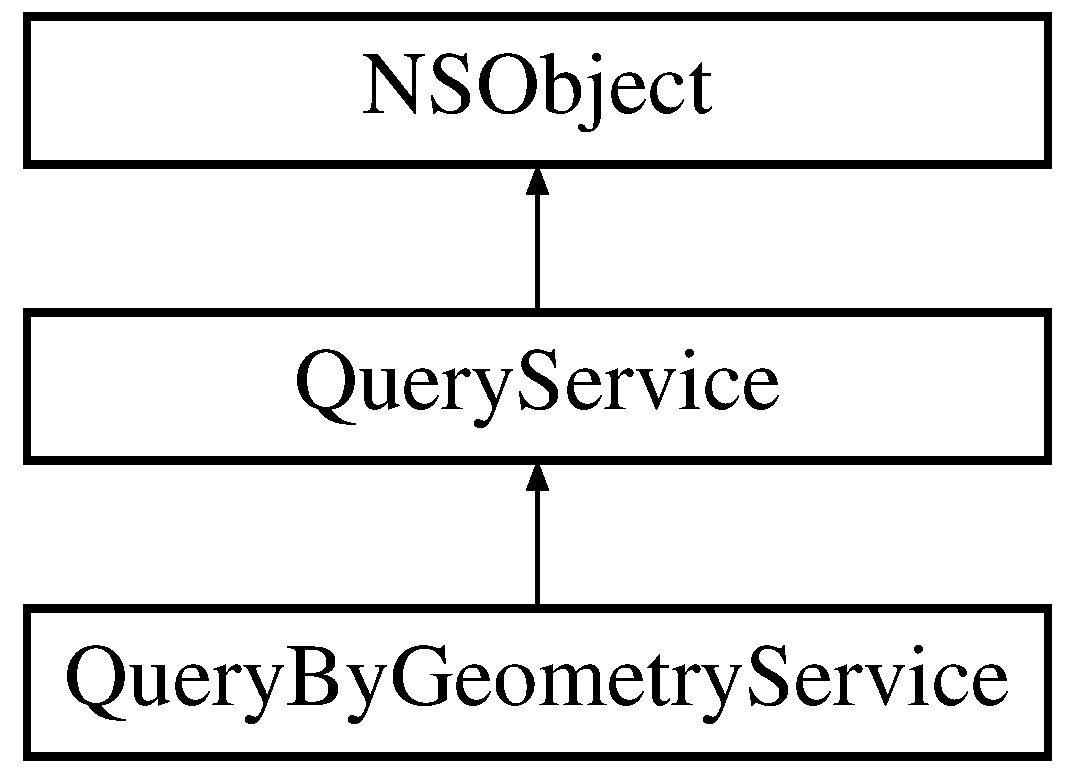
\includegraphics[height=3.000000cm]{interface_query_by_geometry_service}
\end{center}
\end{figure}
\subsection*{Instance Methods}
\begin{DoxyCompactItemize}
\item 
(N\-S\-String $\ast$) -\/ \hyperlink{interface_query_by_geometry_service_a8616e1c52b26452954408aa5a6dea7e2}{get\-Json\-Parameters\-:}
\end{DoxyCompactItemize}
\subsection*{额外继承的成员函数}


\subsection{详细描述}
Geometry 查询服务类。 

\subsection{Method Documentation}
\hypertarget{interface_query_by_geometry_service_a8616e1c52b26452954408aa5a6dea7e2}{\index{Query\-By\-Geometry\-Service@{Query\-By\-Geometry\-Service}!get\-Json\-Parameters\-:@{get\-Json\-Parameters\-:}}
\index{get\-Json\-Parameters\-:@{get\-Json\-Parameters\-:}!QueryByGeometryService@{Query\-By\-Geometry\-Service}}
\subsubsection[{get\-Json\-Parameters\-:}]{\setlength{\rightskip}{0pt plus 5cm}-\/ (N\-S\-String $\ast$) get\-Json\-Parameters\-: 
\begin{DoxyParamCaption}
\item[{({\bf Query\-Parameters}$\ast$)}]{params}
\end{DoxyParamCaption}
}}\label{interface_query_by_geometry_service_a8616e1c52b26452954408aa5a6dea7e2}


该类的文档由以下文件生成\-:\begin{DoxyCompactItemize}
\item 
Map/\hyperlink{_query_by_geometry_service_8h}{Query\-By\-Geometry\-Service.\-h}\item 
Map/\hyperlink{_query_by_geometry_service_8m}{Query\-By\-Geometry\-Service.\-m}\end{DoxyCompactItemize}

\hypertarget{interface_query_by_s_q_l_parameters}{\section{Query\-By\-S\-Q\-L\-Parameters类 参考}
\label{interface_query_by_s_q_l_parameters}\index{Query\-By\-S\-Q\-L\-Parameters@{Query\-By\-S\-Q\-L\-Parameters}}
}


S\-Q\-L 查询参数类。\par
 该类用于设置 S\-Q\-L 查询的相关参数。  




{\ttfamily \#import $<$Query\-By\-S\-Q\-L\-Parameters.\-h$>$}

类 Query\-By\-S\-Q\-L\-Parameters 继承关系图\-:\begin{figure}[H]
\begin{center}
\leavevmode
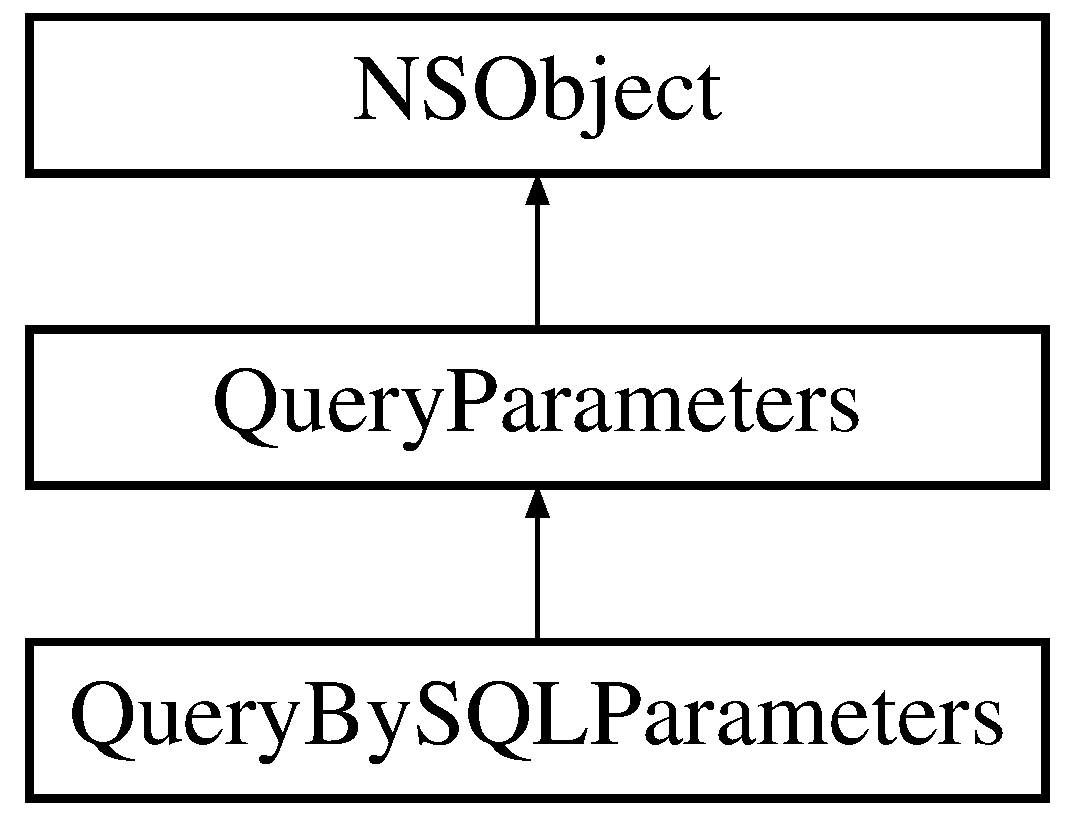
\includegraphics[height=3.000000cm]{interface_query_by_s_q_l_parameters}
\end{center}
\end{figure}
\subsection*{Instance Methods}
\begin{DoxyCompactItemize}
\item 
(id) -\/ \hyperlink{interface_query_by_s_q_l_parameters_a7fd5e1b8332c6d10a5f81f65cc13b284}{init}
\end{DoxyCompactItemize}
\subsection*{额外继承的成员函数}


\subsection{详细描述}
S\-Q\-L 查询参数类。\par
 该类用于设置 S\-Q\-L 查询的相关参数。 

\subsection{Method Documentation}
\hypertarget{interface_query_by_s_q_l_parameters_a7fd5e1b8332c6d10a5f81f65cc13b284}{\index{Query\-By\-S\-Q\-L\-Parameters@{Query\-By\-S\-Q\-L\-Parameters}!init@{init}}
\index{init@{init}!QueryBySQLParameters@{Query\-By\-S\-Q\-L\-Parameters}}
\subsubsection[{init}]{\setlength{\rightskip}{0pt plus 5cm}-\/ (id) init 
\begin{DoxyParamCaption}
{}
\end{DoxyParamCaption}
}}\label{interface_query_by_s_q_l_parameters_a7fd5e1b8332c6d10a5f81f65cc13b284}


重载 \hyperlink{interface_query_parameters_ab34003baea3fb15a37fc89bff33304c3}{Query\-Parameters} .



该类的文档由以下文件生成\-:\begin{DoxyCompactItemize}
\item 
Map/\hyperlink{_query_by_s_q_l_parameters_8h}{Query\-By\-S\-Q\-L\-Parameters.\-h}\item 
Map/\hyperlink{_query_by_s_q_l_parameters_8m}{Query\-By\-S\-Q\-L\-Parameters.\-m}\end{DoxyCompactItemize}

\hypertarget{interface_query_by_s_q_l_service}{\section{Query\-By\-S\-Q\-L\-Service类 参考}
\label{interface_query_by_s_q_l_service}\index{Query\-By\-S\-Q\-L\-Service@{Query\-By\-S\-Q\-L\-Service}}
}


S\-Q\-L 查询服务类。\par
 在一个或多个指定的图层上查询符合 S\-Q\-L 条件的空间地物信息。  




{\ttfamily \#import $<$Query\-By\-S\-Q\-L\-Service.\-h$>$}

类 Query\-By\-S\-Q\-L\-Service 继承关系图\-:\begin{figure}[H]
\begin{center}
\leavevmode
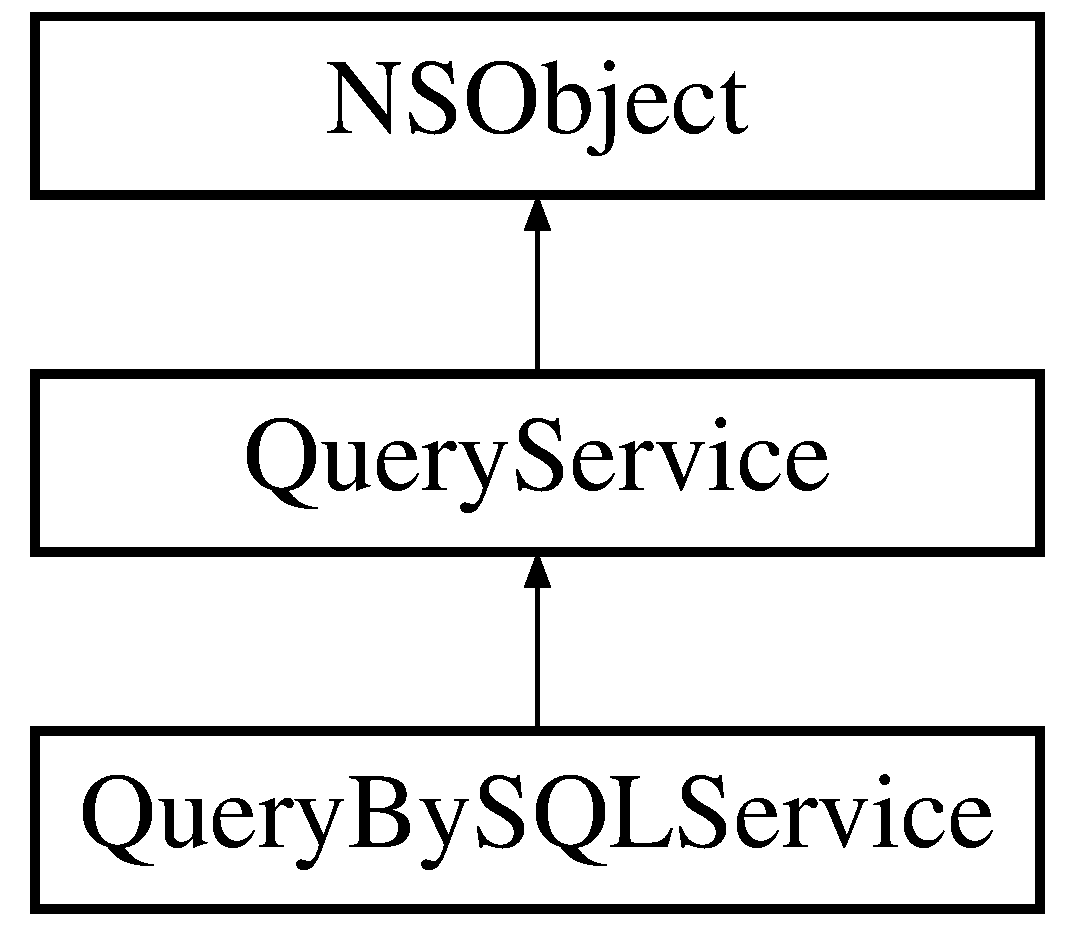
\includegraphics[height=3.000000cm]{interface_query_by_s_q_l_service}
\end{center}
\end{figure}
\subsection*{Instance Methods}
\begin{DoxyCompactItemize}
\item 
(N\-S\-String $\ast$) -\/ \hyperlink{interface_query_by_s_q_l_service_a00bfb7c55f1d2b47178513e5978cbb03}{get\-Json\-Parameters\-:}
\end{DoxyCompactItemize}
\subsection*{额外继承的成员函数}


\subsection{详细描述}
S\-Q\-L 查询服务类。\par
 在一个或多个指定的图层上查询符合 S\-Q\-L 条件的空间地物信息。 

\subsection{Method Documentation}
\hypertarget{interface_query_by_s_q_l_service_a00bfb7c55f1d2b47178513e5978cbb03}{\index{Query\-By\-S\-Q\-L\-Service@{Query\-By\-S\-Q\-L\-Service}!get\-Json\-Parameters\-:@{get\-Json\-Parameters\-:}}
\index{get\-Json\-Parameters\-:@{get\-Json\-Parameters\-:}!QueryBySQLService@{Query\-By\-S\-Q\-L\-Service}}
\subsubsection[{get\-Json\-Parameters\-:}]{\setlength{\rightskip}{0pt plus 5cm}-\/ (N\-S\-String $\ast$) get\-Json\-Parameters\-: 
\begin{DoxyParamCaption}
\item[{({\bf Query\-Parameters}$\ast$)}]{params}
\end{DoxyParamCaption}
}}\label{interface_query_by_s_q_l_service_a00bfb7c55f1d2b47178513e5978cbb03}


该类的文档由以下文件生成\-:\begin{DoxyCompactItemize}
\item 
Map/\hyperlink{_query_by_s_q_l_service_8h}{Query\-By\-S\-Q\-L\-Service.\-h}\item 
Map/\hyperlink{_query_by_s_q_l_service_8m}{Query\-By\-S\-Q\-L\-Service.\-m}\end{DoxyCompactItemize}

\hypertarget{interface_query_parameters}{\section{Query\-Parameters类 参考}
\label{interface_query_parameters}\index{Query\-Parameters@{Query\-Parameters}}
}


查询参数基类。\par
 距离查询、\-S\-Q\-L 查询、几何地物查询等各自的参数均继承此类。  




{\ttfamily \#import $<$Query\-Parameters.\-h$>$}

类 Query\-Parameters 继承关系图\-:\begin{figure}[H]
\begin{center}
\leavevmode
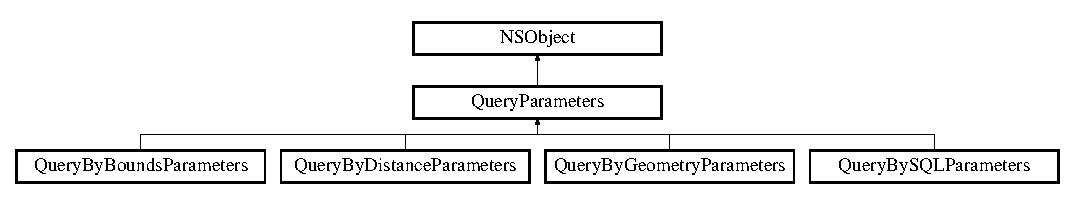
\includegraphics[height=2.222222cm]{interface_query_parameters}
\end{center}
\end{figure}
\subsection*{Instance Methods}
\begin{DoxyCompactItemize}
\item 
(id) -\/ \hyperlink{interface_query_parameters_ab34003baea3fb15a37fc89bff33304c3}{init}{\ttfamily  \mbox{[}implementation\mbox{]}}
\item 
(N\-S\-Mutable\-Dictionary $\ast$) -\/ \hyperlink{interface_query_parameters_a2c76ebeaa300c4397083ba6d5e225f59}{to\-N\-S\-Dictionary}
\end{DoxyCompactItemize}
\subsection*{属性}
\begin{DoxyCompactItemize}
\item 
N\-S\-String $\ast$ \hyperlink{interface_query_parameters_a0fe9432e38283f513ce7498c56fdbc45}{custom\-Params}
\item 
int \hyperlink{interface_query_parameters_a4abfc354c0a5521456ad3c80fc47ad99}{expect\-Count}
\item 
int \hyperlink{interface_query_parameters_a66303e1291da38620e0251c251ec970b}{hold\-Time}
\item 
N\-S\-String $\ast$ \hyperlink{interface_query_parameters_a97094cdc3ba9da5c8b62b9c1b03fccfd}{network\-Type}
\item 
N\-S\-String $\ast$ \hyperlink{interface_query_parameters_a62aa18d0e7ff37366e5b98491fd61068}{query\-Option}
\item 
N\-S\-Mutable\-Array $\ast$ \hyperlink{interface_query_parameters_a83a59495a5d42b0d0e14e09c1c1b3697}{query\-Params}
\item 
B\-O\-O\-L \hyperlink{interface_query_parameters_a23d9965d1a1aa8ff9626f1a0b2abf85c}{return\-Content}
\item 
B\-O\-O\-L \hyperlink{interface_query_parameters_ab62ff61d19899b96890efb932bf8c90a}{return\-Custom\-Result}
\item 
int \hyperlink{interface_query_parameters_adf4931c1732408ec8f3406a788850985}{start\-Record}
\end{DoxyCompactItemize}


\subsection{详细描述}
查询参数基类。\par
 距离查询、\-S\-Q\-L 查询、几何地物查询等各自的参数均继承此类。 

\subsection{Method Documentation}
\hypertarget{interface_query_parameters_ab34003baea3fb15a37fc89bff33304c3}{\index{Query\-Parameters@{Query\-Parameters}!init@{init}}
\index{init@{init}!QueryParameters@{Query\-Parameters}}
\subsubsection[{init}]{\setlength{\rightskip}{0pt plus 5cm}-\/ (id) init 
\begin{DoxyParamCaption}
{}
\end{DoxyParamCaption}
\hspace{0.3cm}{\ttfamily [implementation]}}}\label{interface_query_parameters_ab34003baea3fb15a37fc89bff33304c3}


被 \hyperlink{interface_query_by_s_q_l_parameters_a7fd5e1b8332c6d10a5f81f65cc13b284}{Query\-By\-S\-Q\-L\-Parameters} 重载.



参考自 Query\-By\-Bounds\-Parameters\-::init\-:, Query\-By\-Geometry\-Parameters\-::init\-: , 以及 Query\-By\-Distance\-Parameters\-::init\-:m\-Geometry\-:b\-Nearest\-:.

\hypertarget{interface_query_parameters_a2c76ebeaa300c4397083ba6d5e225f59}{\index{Query\-Parameters@{Query\-Parameters}!to\-N\-S\-Dictionary@{to\-N\-S\-Dictionary}}
\index{to\-N\-S\-Dictionary@{to\-N\-S\-Dictionary}!QueryParameters@{Query\-Parameters}}
\subsubsection[{to\-N\-S\-Dictionary}]{\setlength{\rightskip}{0pt plus 5cm}-\/ (N\-S\-Mutable\-Dictionary $\ast$) to\-N\-S\-Dictionary 
\begin{DoxyParamCaption}
{}
\end{DoxyParamCaption}
}}\label{interface_query_parameters_a2c76ebeaa300c4397083ba6d5e225f59}


参考自 Query\-By\-Bounds\-Service\-::get\-Json\-Parameters\-:, Query\-By\-S\-Q\-L\-Service\-::get\-Json\-Parameters\-:, Query\-By\-Geometry\-Service\-::get\-Json\-Parameters\-: , 以及 Query\-By\-Distance\-Service\-::get\-Json\-Parameters\-:.



\subsection{属性说明}
\hypertarget{interface_query_parameters_a0fe9432e38283f513ce7498c56fdbc45}{\index{Query\-Parameters@{Query\-Parameters}!custom\-Params@{custom\-Params}}
\index{custom\-Params@{custom\-Params}!QueryParameters@{Query\-Parameters}}
\subsubsection[{custom\-Params}]{\setlength{\rightskip}{0pt plus 5cm}-\/ (N\-S\-String $\ast$) custom\-Params\hspace{0.3cm}{\ttfamily [read]}, {\ttfamily [write]}, {\ttfamily [atomic]}, {\ttfamily [copy]}}}\label{interface_query_parameters_a0fe9432e38283f513ce7498c56fdbc45}


参考自 Query\-Service\-::get\-Query\-Parameters\-: , 以及 init.

\hypertarget{interface_query_parameters_a4abfc354c0a5521456ad3c80fc47ad99}{\index{Query\-Parameters@{Query\-Parameters}!expect\-Count@{expect\-Count}}
\index{expect\-Count@{expect\-Count}!QueryParameters@{Query\-Parameters}}
\subsubsection[{expect\-Count}]{\setlength{\rightskip}{0pt plus 5cm}-\/ (int) expect\-Count\hspace{0.3cm}{\ttfamily [read]}, {\ttfamily [write]}, {\ttfamily [atomic]}, {\ttfamily [assign]}}}\label{interface_query_parameters_a4abfc354c0a5521456ad3c80fc47ad99}


参考自 Query\-Service\-::get\-Query\-Parameters\-: , 以及 init.

\hypertarget{interface_query_parameters_a66303e1291da38620e0251c251ec970b}{\index{Query\-Parameters@{Query\-Parameters}!hold\-Time@{hold\-Time}}
\index{hold\-Time@{hold\-Time}!QueryParameters@{Query\-Parameters}}
\subsubsection[{hold\-Time}]{\setlength{\rightskip}{0pt plus 5cm}-\/ (int) hold\-Time\hspace{0.3cm}{\ttfamily [read]}, {\ttfamily [write]}, {\ttfamily [atomic]}, {\ttfamily [assign]}}}\label{interface_query_parameters_a66303e1291da38620e0251c251ec970b}


参考自 Query\-Service\-::get\-Query\-Parameters\-: , 以及 init.

\hypertarget{interface_query_parameters_a97094cdc3ba9da5c8b62b9c1b03fccfd}{\index{Query\-Parameters@{Query\-Parameters}!network\-Type@{network\-Type}}
\index{network\-Type@{network\-Type}!QueryParameters@{Query\-Parameters}}
\subsubsection[{network\-Type}]{\setlength{\rightskip}{0pt plus 5cm}-\/ (N\-S\-String $\ast$) network\-Type\hspace{0.3cm}{\ttfamily [read]}, {\ttfamily [write]}, {\ttfamily [atomic]}, {\ttfamily [copy]}}}\label{interface_query_parameters_a97094cdc3ba9da5c8b62b9c1b03fccfd}


参考自 Query\-Service\-::get\-Query\-Parameters\-: , 以及 init.

\hypertarget{interface_query_parameters_a62aa18d0e7ff37366e5b98491fd61068}{\index{Query\-Parameters@{Query\-Parameters}!query\-Option@{query\-Option}}
\index{query\-Option@{query\-Option}!QueryParameters@{Query\-Parameters}}
\subsubsection[{query\-Option}]{\setlength{\rightskip}{0pt plus 5cm}-\/ (N\-S\-String $\ast$) query\-Option\hspace{0.3cm}{\ttfamily [read]}, {\ttfamily [write]}, {\ttfamily [atomic]}, {\ttfamily [copy]}}}\label{interface_query_parameters_a62aa18d0e7ff37366e5b98491fd61068}


参考自 Query\-Service\-::get\-Query\-Parameters\-: , 以及 init.

\hypertarget{interface_query_parameters_a83a59495a5d42b0d0e14e09c1c1b3697}{\index{Query\-Parameters@{Query\-Parameters}!query\-Params@{query\-Params}}
\index{query\-Params@{query\-Params}!QueryParameters@{Query\-Parameters}}
\subsubsection[{query\-Params}]{\setlength{\rightskip}{0pt plus 5cm}-\/ (N\-S\-Mutable\-Array $\ast$) query\-Params\hspace{0.3cm}{\ttfamily [read]}, {\ttfamily [write]}, {\ttfamily [atomic]}, {\ttfamily [copy]}}}\label{interface_query_parameters_a83a59495a5d42b0d0e14e09c1c1b3697}


参考自 Query\-Service\-::get\-Query\-Parameters\-:, init , 以及 to\-N\-S\-Dictionary.

\hypertarget{interface_query_parameters_a23d9965d1a1aa8ff9626f1a0b2abf85c}{\index{Query\-Parameters@{Query\-Parameters}!return\-Content@{return\-Content}}
\index{return\-Content@{return\-Content}!QueryParameters@{Query\-Parameters}}
\subsubsection[{return\-Content}]{\setlength{\rightskip}{0pt plus 5cm}-\/ (B\-O\-O\-L) return\-Content\hspace{0.3cm}{\ttfamily [read]}, {\ttfamily [write]}, {\ttfamily [atomic]}, {\ttfamily [assign]}}}\label{interface_query_parameters_a23d9965d1a1aa8ff9626f1a0b2abf85c}


参考自 init.

\hypertarget{interface_query_parameters_ab62ff61d19899b96890efb932bf8c90a}{\index{Query\-Parameters@{Query\-Parameters}!return\-Custom\-Result@{return\-Custom\-Result}}
\index{return\-Custom\-Result@{return\-Custom\-Result}!QueryParameters@{Query\-Parameters}}
\subsubsection[{return\-Custom\-Result}]{\setlength{\rightskip}{0pt plus 5cm}-\/ (B\-O\-O\-L) return\-Custom\-Result\hspace{0.3cm}{\ttfamily [read]}, {\ttfamily [atomic]}, {\ttfamily [assign]}}}\label{interface_query_parameters_ab62ff61d19899b96890efb932bf8c90a}


参考自 init.

\hypertarget{interface_query_parameters_adf4931c1732408ec8f3406a788850985}{\index{Query\-Parameters@{Query\-Parameters}!start\-Record@{start\-Record}}
\index{start\-Record@{start\-Record}!QueryParameters@{Query\-Parameters}}
\subsubsection[{start\-Record}]{\setlength{\rightskip}{0pt plus 5cm}-\/ (int) start\-Record\hspace{0.3cm}{\ttfamily [read]}, {\ttfamily [write]}, {\ttfamily [atomic]}, {\ttfamily [assign]}}}\label{interface_query_parameters_adf4931c1732408ec8f3406a788850985}


参考自 Query\-Service\-::get\-Query\-Parameters\-: , 以及 init.



该类的文档由以下文件生成\-:\begin{DoxyCompactItemize}
\item 
Map/\hyperlink{_query_parameters_8h}{Query\-Parameters.\-h}\item 
Map/\hyperlink{_query_parameters_8m}{Query\-Parameters.\-m}\end{DoxyCompactItemize}

\hypertarget{interface_query_result}{\section{Query\-Result类 参考}
\label{interface_query_result}\index{Query\-Result@{Query\-Result}}
}


查询结果类。\par
 查询结果类中包含了查询结果记录集(\-Recordset)或查询结果资源(\-Resource\-Info)的相关信息。  




{\ttfamily \#import $<$Query\-Result.\-h$>$}

类 Query\-Result 继承关系图\-:\begin{figure}[H]
\begin{center}
\leavevmode
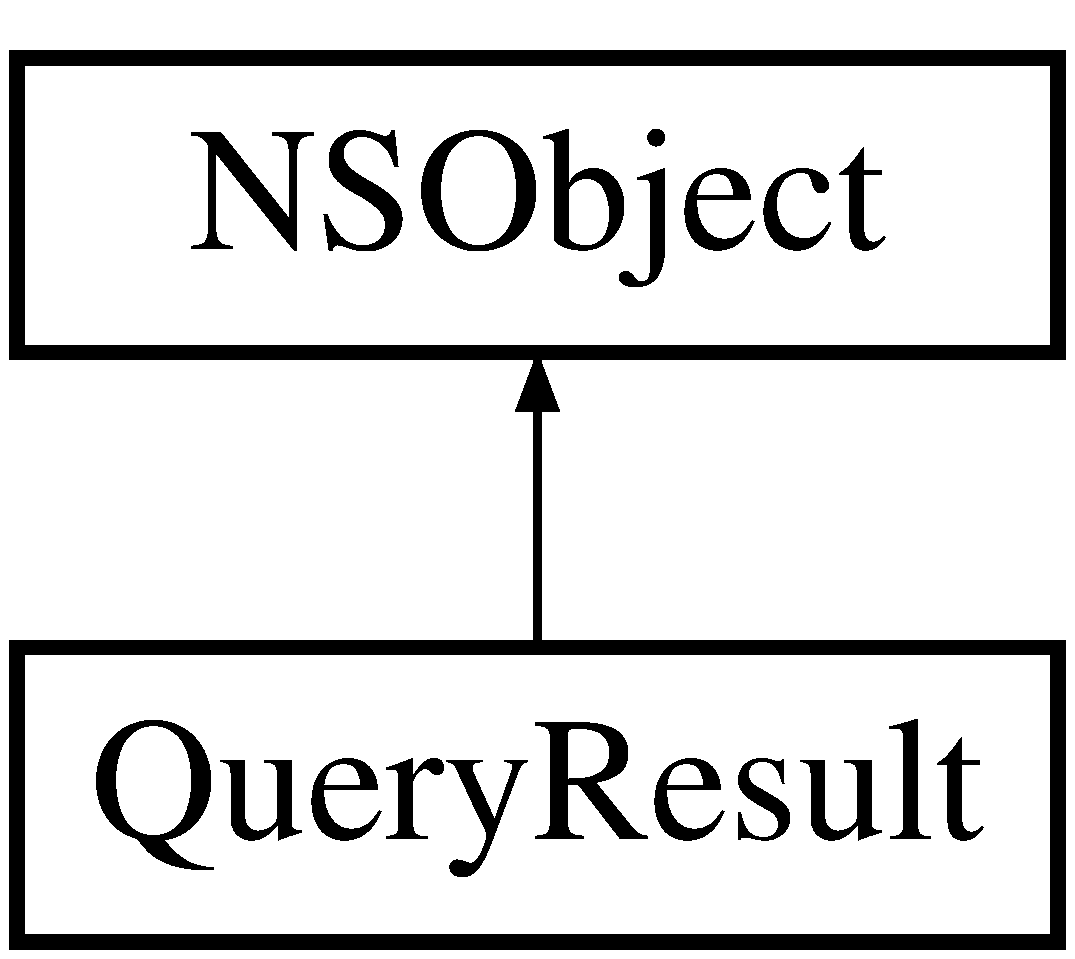
\includegraphics[height=2.000000cm]{interface_query_result}
\end{center}
\end{figure}
\subsection*{Instance Methods}
\begin{DoxyCompactItemize}
\item 
(void) -\/ \hyperlink{interface_query_result_a7b544bf7eda0db130df7a168024f1705}{from\-Json\-:}
\end{DoxyCompactItemize}
\subsection*{属性}
\begin{DoxyCompactItemize}
\item 
int \hyperlink{interface_query_result_ae765c93f480df132156e52d30bdba658}{current\-Count}
\item 
id \hyperlink{interface_query_result_af268ab97cb214a7c2ef2b8051904d171}{custom\-Response}
\item 
N\-S\-Mutable\-Array $\ast$ \hyperlink{interface_query_result_aafa1ccf4b6f17ccf7eb40a9065fc2331}{recordsets}
\item 
int \hyperlink{interface_query_result_a8b261d4cb2e36b27791f064789c8644b}{total\-Count}
\end{DoxyCompactItemize}


\subsection{详细描述}
查询结果类。\par
 查询结果类中包含了查询结果记录集(\-Recordset)或查询结果资源(\-Resource\-Info)的相关信息。 

\subsection{Method Documentation}
\hypertarget{interface_query_result_a7b544bf7eda0db130df7a168024f1705}{\index{Query\-Result@{Query\-Result}!from\-Json\-:@{from\-Json\-:}}
\index{from\-Json\-:@{from\-Json\-:}!QueryResult@{Query\-Result}}
\subsubsection[{from\-Json\-:}]{\setlength{\rightskip}{0pt plus 5cm}-\/ (void) from\-Json\-: 
\begin{DoxyParamCaption}
\item[{(N\-S\-String$\ast$)}]{str\-Json}
\end{DoxyParamCaption}
}}\label{interface_query_result_a7b544bf7eda0db130df7a168024f1705}


参考自 Query\-Service\-::connection\-Did\-Finish\-Loading\-:.



\subsection{属性说明}
\hypertarget{interface_query_result_ae765c93f480df132156e52d30bdba658}{\index{Query\-Result@{Query\-Result}!current\-Count@{current\-Count}}
\index{current\-Count@{current\-Count}!QueryResult@{Query\-Result}}
\subsubsection[{current\-Count}]{\setlength{\rightskip}{0pt plus 5cm}-\/ (int) current\-Count\hspace{0.3cm}{\ttfamily [read]}, {\ttfamily [write]}, {\ttfamily [atomic]}, {\ttfamily [assign]}}}\label{interface_query_result_ae765c93f480df132156e52d30bdba658}


参考自 from\-Json\-:.

\hypertarget{interface_query_result_af268ab97cb214a7c2ef2b8051904d171}{\index{Query\-Result@{Query\-Result}!custom\-Response@{custom\-Response}}
\index{custom\-Response@{custom\-Response}!QueryResult@{Query\-Result}}
\subsubsection[{custom\-Response}]{\setlength{\rightskip}{0pt plus 5cm}-\/ (id) custom\-Response\hspace{0.3cm}{\ttfamily [read]}, {\ttfamily [write]}, {\ttfamily [atomic]}, {\ttfamily [copy]}}}\label{interface_query_result_af268ab97cb214a7c2ef2b8051904d171}


参考自 from\-Json\-:.

\hypertarget{interface_query_result_aafa1ccf4b6f17ccf7eb40a9065fc2331}{\index{Query\-Result@{Query\-Result}!recordsets@{recordsets}}
\index{recordsets@{recordsets}!QueryResult@{Query\-Result}}
\subsubsection[{recordsets}]{\setlength{\rightskip}{0pt plus 5cm}-\/ (N\-S\-Mutable\-Array $\ast$) recordsets\hspace{0.3cm}{\ttfamily [read]}, {\ttfamily [write]}, {\ttfamily [atomic]}, {\ttfamily [retain]}}}\label{interface_query_result_aafa1ccf4b6f17ccf7eb40a9065fc2331}


参考自 from\-Json\-:.

\hypertarget{interface_query_result_a8b261d4cb2e36b27791f064789c8644b}{\index{Query\-Result@{Query\-Result}!total\-Count@{total\-Count}}
\index{total\-Count@{total\-Count}!QueryResult@{Query\-Result}}
\subsubsection[{total\-Count}]{\setlength{\rightskip}{0pt plus 5cm}-\/ (int) total\-Count\hspace{0.3cm}{\ttfamily [read]}, {\ttfamily [write]}, {\ttfamily [atomic]}, {\ttfamily [assign]}}}\label{interface_query_result_a8b261d4cb2e36b27791f064789c8644b}


参考自 from\-Json\-:.



该类的文档由以下文件生成\-:\begin{DoxyCompactItemize}
\item 
Map/\hyperlink{_query_result_8h}{Query\-Result.\-h}\item 
Map/\hyperlink{_query_result_8m}{Query\-Result.\-m}\end{DoxyCompactItemize}

\hypertarget{interface_query_service}{\section{Query\-Service类 参考}
\label{interface_query_service}\index{Query\-Service@{Query\-Service}}
}


{\ttfamily \#import $<$Query\-Service.\-h$>$}

类 Query\-Service 继承关系图\-:\begin{figure}[H]
\begin{center}
\leavevmode
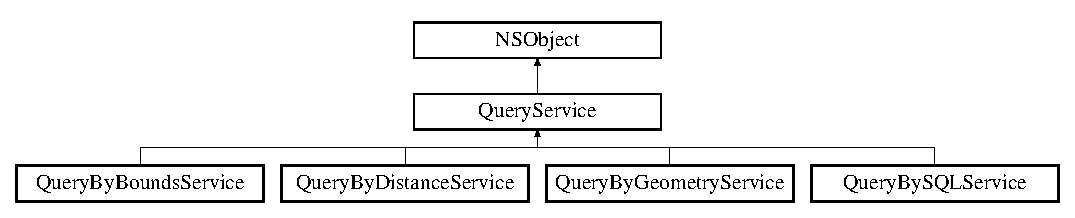
\includegraphics[height=2.485207cm]{interface_query_service}
\end{center}
\end{figure}
\subsection*{Instance Methods}
\begin{DoxyCompactItemize}
\item 
(void) -\/ \hyperlink{interface_query_service_a98be7666a9ed5ec6083aee4d72ebc855}{connection\-:did\-Fail\-With\-Error\-:}{\ttfamily  \mbox{[}implementation\mbox{]}}
\item 
(void) -\/ \hyperlink{interface_query_service_a74a40e3c8270e08c175c36f97da4ff2c}{connection\-:did\-Receive\-Data\-:}{\ttfamily  \mbox{[}implementation\mbox{]}}
\item 
(void) -\/ \hyperlink{interface_query_service_ad458e3790d8616a6b0e0d94b378549b0}{connection\-:did\-Receive\-Response\-:}{\ttfamily  \mbox{[}implementation\mbox{]}}
\item 
(void) -\/ \hyperlink{interface_query_service_a817956092252af96bfd27c6fcbc8cf4f}{connection\-Did\-Finish\-Loading\-:}{\ttfamily  \mbox{[}implementation\mbox{]}}
\item 
(\hyperlink{interface_query_parameters}{Query\-Parameters} $\ast$) -\/ \hyperlink{interface_query_service_abeb01f02ddfd9320d881c29b839999a8}{get\-Query\-Parameters\-:}
\item 
(id) -\/ \hyperlink{interface_query_service_a7a0a3055ea245b0602a3604bb2db3094}{init\-:}
\item 
(void) -\/ \hyperlink{interface_query_service_a80a886ec8e3d38d5f35de003220292d3}{process\-Async\-:}
\end{DoxyCompactItemize}
\subsection*{Protected 属性}
\begin{DoxyCompactItemize}
\item 
N\-S\-Mutable\-Data $\ast$ \hyperlink{interface_query_service_aa41069a3a5501c58f1d83d41de743c89}{data}
\item 
N\-S\-String $\ast$ \hyperlink{interface_query_service_a3bded815fbe946f576b68aecd953d43d}{str\-Query\-Url}
\end{DoxyCompactItemize}


\subsection{Method Documentation}
\hypertarget{interface_query_service_a98be7666a9ed5ec6083aee4d72ebc855}{\index{Query\-Service@{Query\-Service}!connection\-:did\-Fail\-With\-Error\-:@{connection\-:did\-Fail\-With\-Error\-:}}
\index{connection\-:did\-Fail\-With\-Error\-:@{connection\-:did\-Fail\-With\-Error\-:}!QueryService@{Query\-Service}}
\subsubsection[{connection\-:did\-Fail\-With\-Error\-:}]{\setlength{\rightskip}{0pt plus 5cm}-\/ (void) connection\-: 
\begin{DoxyParamCaption}
\item[{(N\-S\-U\-R\-L\-Connection $\ast$)}]{connection}
\item[{didFailWithError:(N\-S\-Error $\ast$)}]{error}
\end{DoxyParamCaption}
\hspace{0.3cm}{\ttfamily [implementation]}}}\label{interface_query_service_a98be7666a9ed5ec6083aee4d72ebc855}
\hypertarget{interface_query_service_a74a40e3c8270e08c175c36f97da4ff2c}{\index{Query\-Service@{Query\-Service}!connection\-:did\-Receive\-Data\-:@{connection\-:did\-Receive\-Data\-:}}
\index{connection\-:did\-Receive\-Data\-:@{connection\-:did\-Receive\-Data\-:}!QueryService@{Query\-Service}}
\subsubsection[{connection\-:did\-Receive\-Data\-:}]{\setlength{\rightskip}{0pt plus 5cm}-\/ (void) connection\-: 
\begin{DoxyParamCaption}
\item[{(N\-S\-U\-R\-L\-Connection $\ast$)}]{connection}
\item[{didReceiveData:(N\-S\-Data $\ast$)}]{smdata}
\end{DoxyParamCaption}
\hspace{0.3cm}{\ttfamily [implementation]}}}\label{interface_query_service_a74a40e3c8270e08c175c36f97da4ff2c}
\hypertarget{interface_query_service_ad458e3790d8616a6b0e0d94b378549b0}{\index{Query\-Service@{Query\-Service}!connection\-:did\-Receive\-Response\-:@{connection\-:did\-Receive\-Response\-:}}
\index{connection\-:did\-Receive\-Response\-:@{connection\-:did\-Receive\-Response\-:}!QueryService@{Query\-Service}}
\subsubsection[{connection\-:did\-Receive\-Response\-:}]{\setlength{\rightskip}{0pt plus 5cm}-\/ (void) connection\-: 
\begin{DoxyParamCaption}
\item[{(N\-S\-U\-R\-L\-Connection $\ast$)}]{connection}
\item[{didReceiveResponse:(N\-S\-U\-R\-L\-Response $\ast$)}]{response}
\end{DoxyParamCaption}
\hspace{0.3cm}{\ttfamily [implementation]}}}\label{interface_query_service_ad458e3790d8616a6b0e0d94b378549b0}
\hypertarget{interface_query_service_a817956092252af96bfd27c6fcbc8cf4f}{\index{Query\-Service@{Query\-Service}!connection\-Did\-Finish\-Loading\-:@{connection\-Did\-Finish\-Loading\-:}}
\index{connection\-Did\-Finish\-Loading\-:@{connection\-Did\-Finish\-Loading\-:}!QueryService@{Query\-Service}}
\subsubsection[{connection\-Did\-Finish\-Loading\-:}]{\setlength{\rightskip}{0pt plus 5cm}-\/ (void) connection\-Did\-Finish\-Loading\-: 
\begin{DoxyParamCaption}
\item[{(N\-S\-U\-R\-L\-Connection $\ast$)}]{connection}
\end{DoxyParamCaption}
\hspace{0.3cm}{\ttfamily [implementation]}}}\label{interface_query_service_a817956092252af96bfd27c6fcbc8cf4f}
\hypertarget{interface_query_service_abeb01f02ddfd9320d881c29b839999a8}{\index{Query\-Service@{Query\-Service}!get\-Query\-Parameters\-:@{get\-Query\-Parameters\-:}}
\index{get\-Query\-Parameters\-:@{get\-Query\-Parameters\-:}!QueryService@{Query\-Service}}
\subsubsection[{get\-Query\-Parameters\-:}]{\setlength{\rightskip}{0pt plus 5cm}-\/ ({\bf Query\-Parameters} $\ast$) get\-Query\-Parameters\-: 
\begin{DoxyParamCaption}
\item[{({\bf Query\-Parameters}$\ast$)}]{params}
\end{DoxyParamCaption}
}}\label{interface_query_service_abeb01f02ddfd9320d881c29b839999a8}


参考自 Query\-By\-Bounds\-Service\-::get\-Json\-Parameters\-:, Query\-By\-S\-Q\-L\-Service\-::get\-Json\-Parameters\-:, Query\-By\-Geometry\-Service\-::get\-Json\-Parameters\-: , 以及 Query\-By\-Distance\-Service\-::get\-Json\-Parameters\-:.

\hypertarget{interface_query_service_a7a0a3055ea245b0602a3604bb2db3094}{\index{Query\-Service@{Query\-Service}!init\-:@{init\-:}}
\index{init\-:@{init\-:}!QueryService@{Query\-Service}}
\subsubsection[{init\-:}]{\setlength{\rightskip}{0pt plus 5cm}-\/ (id) init\-: 
\begin{DoxyParamCaption}
\item[{(N\-S\-String$\ast$)}]{str\-Url}
\end{DoxyParamCaption}
}}\label{interface_query_service_a7a0a3055ea245b0602a3604bb2db3094}
\hypertarget{interface_query_service_a80a886ec8e3d38d5f35de003220292d3}{\index{Query\-Service@{Query\-Service}!process\-Async\-:@{process\-Async\-:}}
\index{process\-Async\-:@{process\-Async\-:}!QueryService@{Query\-Service}}
\subsubsection[{process\-Async\-:}]{\setlength{\rightskip}{0pt plus 5cm}-\/ (void) process\-Async\-: 
\begin{DoxyParamCaption}
\item[{({\bf Query\-Parameters}$\ast$)}]{params}
\end{DoxyParamCaption}
}}\label{interface_query_service_a80a886ec8e3d38d5f35de003220292d3}


\subsection{类成员变量说明}
\hypertarget{interface_query_service_aa41069a3a5501c58f1d83d41de743c89}{\index{Query\-Service@{Query\-Service}!data@{data}}
\index{data@{data}!QueryService@{Query\-Service}}
\subsubsection[{data}]{\setlength{\rightskip}{0pt plus 5cm}-\/ (N\-S\-Mutable\-Data$\ast$) data\hspace{0.3cm}{\ttfamily [protected]}}}\label{interface_query_service_aa41069a3a5501c58f1d83d41de743c89}


参考自 connection\-:did\-Receive\-Data\-:, connection\-:did\-Receive\-Response\-: , 以及 process\-Async\-:.

\hypertarget{interface_query_service_a3bded815fbe946f576b68aecd953d43d}{\index{Query\-Service@{Query\-Service}!str\-Query\-Url@{str\-Query\-Url}}
\index{str\-Query\-Url@{str\-Query\-Url}!QueryService@{Query\-Service}}
\subsubsection[{str\-Query\-Url}]{\setlength{\rightskip}{0pt plus 5cm}-\/ (N\-S\-String$\ast$) str\-Query\-Url\hspace{0.3cm}{\ttfamily [protected]}}}\label{interface_query_service_a3bded815fbe946f576b68aecd953d43d}


参考自 init\-:.



该类的文档由以下文件生成\-:\begin{DoxyCompactItemize}
\item 
Map/\hyperlink{_query_service_8h}{Query\-Service.\-h}\item 
Map/\hyperlink{_query_service_8m}{Query\-Service.\-m}\end{DoxyCompactItemize}

\hypertarget{protocol_query_service-p}{\section{$<$Query\-Service$>$协议 参考}
\label{protocol_query_service-p}\index{$<$\-Query\-Service$>$@{$<$\-Query\-Service$>$}}
}


查询服务基类。  




{\ttfamily \#import $<$Query\-Service.\-h$>$}

\subsection*{Instance Methods}
\begin{DoxyCompactItemize}
\item 
(N\-S\-String $\ast$) -\/ \hyperlink{protocol_query_service-p_aed8380afa484ab92d7958f6e0e693ddf}{get\-Json\-Parameters\-:}
\end{DoxyCompactItemize}


\subsection{详细描述}
查询服务基类。 

\subsection{Method Documentation}
\hypertarget{protocol_query_service-p_aed8380afa484ab92d7958f6e0e693ddf}{\index{Query\-Service-\/p@{Query\-Service-\/p}!get\-Json\-Parameters\-:@{get\-Json\-Parameters\-:}}
\index{get\-Json\-Parameters\-:@{get\-Json\-Parameters\-:}!QueryService-p@{Query\-Service-\/p}}
\subsubsection[{get\-Json\-Parameters\-:}]{\setlength{\rightskip}{0pt plus 5cm}-\/ (N\-S\-String$\ast$) get\-Json\-Parameters\-: 
\begin{DoxyParamCaption}
\item[{({\bf Query\-Parameters} $\ast$)}]{params}
\end{DoxyParamCaption}
}}\label{protocol_query_service-p_aed8380afa484ab92d7958f6e0e693ddf}


该协议的文档由以下文件生成\-:\begin{DoxyCompactItemize}
\item 
Map/\hyperlink{_query_service_8h}{Query\-Service.\-h}\end{DoxyCompactItemize}

\hypertarget{interface_recordset}{\section{Recordset类 参考}
\label{interface_recordset}\index{Recordset@{Recordset}}
}


查询结果记录集 \par
 将查询出来的地物按照图层进行划分,一个查询记录集存放一个图层的查询结果, 即查询出的所有地物要素。  




{\ttfamily \#import $<$Recordset.\-h$>$}

类 Recordset 继承关系图\-:\begin{figure}[H]
\begin{center}
\leavevmode
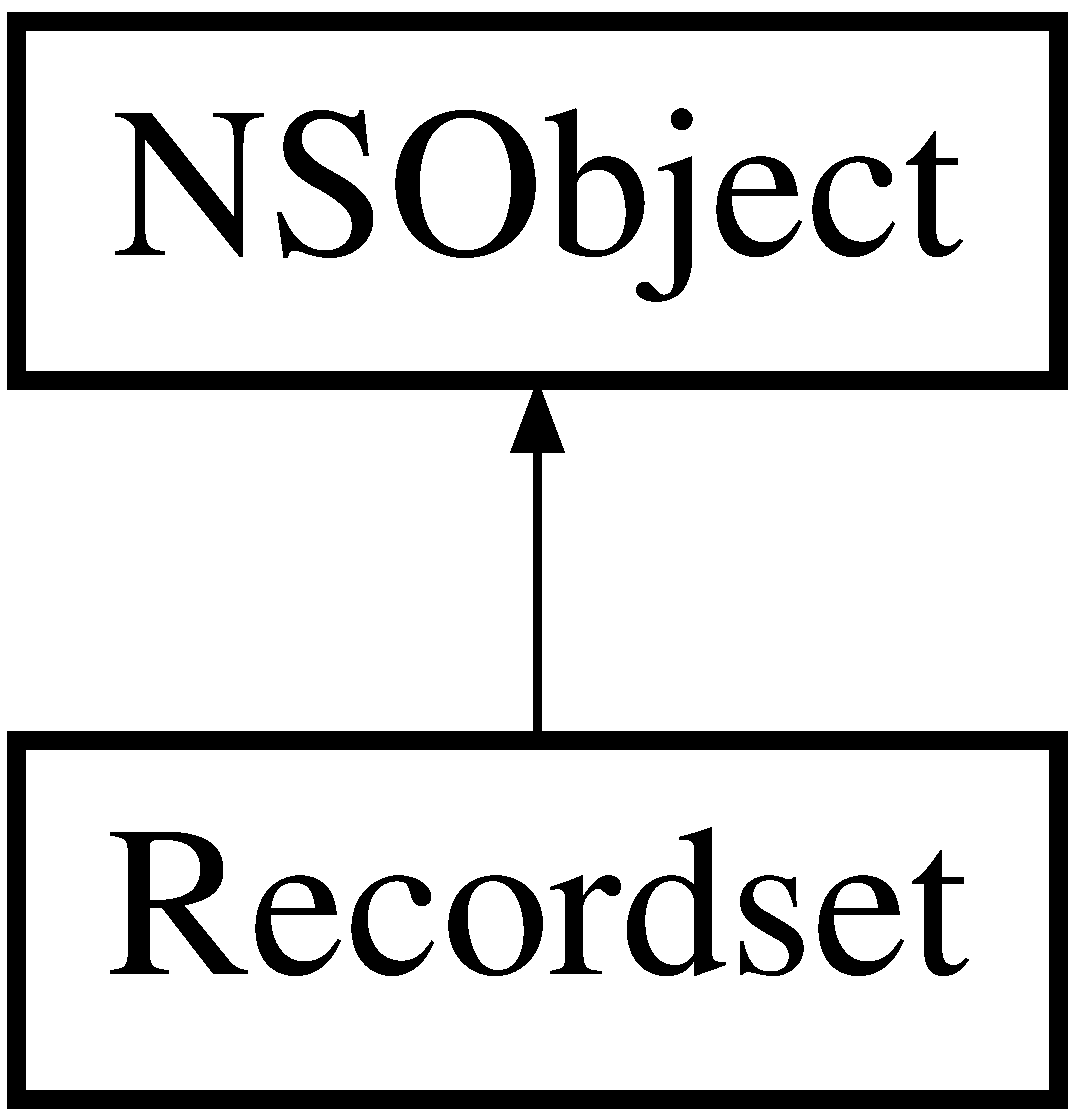
\includegraphics[height=2.000000cm]{interface_recordset}
\end{center}
\end{figure}
\subsection*{Instance Methods}
\begin{DoxyCompactItemize}
\item 
(id) -\/ \hyperlink{interface_recordset_a36686a883d12b9134ad587da12cc4c6d}{initfrom\-Json\-:}
\end{DoxyCompactItemize}
\subsection*{属性}
\begin{DoxyCompactItemize}
\item 
N\-S\-String $\ast$ \hyperlink{interface_recordset_a17a7ab051b651a983c392452eceb0b28}{dataset\-Name}
\item 
N\-S\-Mutable\-Array $\ast$ \hyperlink{interface_recordset_ae6f0e40fdc04c4e63a62e8be7480625e}{features}
\item 
N\-S\-Mutable\-Array $\ast$ \hyperlink{interface_recordset_aa6c80a7cd4d52f37f5e840fa7ca85210}{field\-Captions}
\item 
N\-S\-Mutable\-Array $\ast$ \hyperlink{interface_recordset_ae20147a35c4cb7ef4601143e905472c8}{fields}
\item 
N\-S\-Mutable\-Array $\ast$ \hyperlink{interface_recordset_a08619b9dcb3f4bd54d8fb3c0a1059d85}{field\-Types}
\end{DoxyCompactItemize}


\subsection{详细描述}
查询结果记录集 \par
 将查询出来的地物按照图层进行划分,一个查询记录集存放一个图层的查询结果, 即查询出的所有地物要素。 

\subsection{Method Documentation}
\hypertarget{interface_recordset_a36686a883d12b9134ad587da12cc4c6d}{\index{Recordset@{Recordset}!initfrom\-Json\-:@{initfrom\-Json\-:}}
\index{initfrom\-Json\-:@{initfrom\-Json\-:}!Recordset@{Recordset}}
\subsubsection[{initfrom\-Json\-:}]{\setlength{\rightskip}{0pt plus 5cm}-\/ (id) initfrom\-Json\-: 
\begin{DoxyParamCaption}
\item[{(N\-S\-Dictionary$\ast$)}]{str\-Json}
\end{DoxyParamCaption}
}}\label{interface_recordset_a36686a883d12b9134ad587da12cc4c6d}


\subsection{属性说明}
\hypertarget{interface_recordset_a17a7ab051b651a983c392452eceb0b28}{\index{Recordset@{Recordset}!dataset\-Name@{dataset\-Name}}
\index{dataset\-Name@{dataset\-Name}!Recordset@{Recordset}}
\subsubsection[{dataset\-Name}]{\setlength{\rightskip}{0pt plus 5cm}-\/ (N\-S\-String $\ast$) dataset\-Name\hspace{0.3cm}{\ttfamily [read]}, {\ttfamily [write]}, {\ttfamily [atomic]}, {\ttfamily [copy]}}}\label{interface_recordset_a17a7ab051b651a983c392452eceb0b28}


参考自 initfrom\-Json\-:.

\hypertarget{interface_recordset_ae6f0e40fdc04c4e63a62e8be7480625e}{\index{Recordset@{Recordset}!features@{features}}
\index{features@{features}!Recordset@{Recordset}}
\subsubsection[{features}]{\setlength{\rightskip}{0pt plus 5cm}-\/ (N\-S\-Mutable\-Array $\ast$) features\hspace{0.3cm}{\ttfamily [read]}, {\ttfamily [write]}, {\ttfamily [atomic]}, {\ttfamily [retain]}}}\label{interface_recordset_ae6f0e40fdc04c4e63a62e8be7480625e}


参考自 initfrom\-Json\-:.

\hypertarget{interface_recordset_aa6c80a7cd4d52f37f5e840fa7ca85210}{\index{Recordset@{Recordset}!field\-Captions@{field\-Captions}}
\index{field\-Captions@{field\-Captions}!Recordset@{Recordset}}
\subsubsection[{field\-Captions}]{\setlength{\rightskip}{0pt plus 5cm}-\/ (N\-S\-Mutable\-Array $\ast$) field\-Captions\hspace{0.3cm}{\ttfamily [read]}, {\ttfamily [write]}, {\ttfamily [atomic]}, {\ttfamily [retain]}}}\label{interface_recordset_aa6c80a7cd4d52f37f5e840fa7ca85210}


参考自 initfrom\-Json\-:.

\hypertarget{interface_recordset_ae20147a35c4cb7ef4601143e905472c8}{\index{Recordset@{Recordset}!fields@{fields}}
\index{fields@{fields}!Recordset@{Recordset}}
\subsubsection[{fields}]{\setlength{\rightskip}{0pt plus 5cm}-\/ (N\-S\-Mutable\-Array $\ast$) fields\hspace{0.3cm}{\ttfamily [read]}, {\ttfamily [write]}, {\ttfamily [atomic]}, {\ttfamily [retain]}}}\label{interface_recordset_ae20147a35c4cb7ef4601143e905472c8}


参考自 initfrom\-Json\-:.

\hypertarget{interface_recordset_a08619b9dcb3f4bd54d8fb3c0a1059d85}{\index{Recordset@{Recordset}!field\-Types@{field\-Types}}
\index{field\-Types@{field\-Types}!Recordset@{Recordset}}
\subsubsection[{field\-Types}]{\setlength{\rightskip}{0pt plus 5cm}-\/ (N\-S\-Mutable\-Array $\ast$) field\-Types\hspace{0.3cm}{\ttfamily [read]}, {\ttfamily [write]}, {\ttfamily [atomic]}, {\ttfamily [retain]}}}\label{interface_recordset_a08619b9dcb3f4bd54d8fb3c0a1059d85}


参考自 initfrom\-Json\-:.



该类的文档由以下文件生成\-:\begin{DoxyCompactItemize}
\item 
Map/\hyperlink{_recordset_8h}{Recordset.\-h}\item 
Map/\hyperlink{_recordset_8m}{Recordset.\-m}\end{DoxyCompactItemize}

\hypertarget{interface_r_m_abstract_mercator_web_source}{\section{R\-M\-Abstract\-Mercator\-Web\-Source类 参考}
\label{interface_r_m_abstract_mercator_web_source}\index{R\-M\-Abstract\-Mercator\-Web\-Source@{R\-M\-Abstract\-Mercator\-Web\-Source}}
}


{\ttfamily \#import $<$R\-M\-Abstract\-Mercator\-Web\-Source.\-h$>$}

类 R\-M\-Abstract\-Mercator\-Web\-Source 继承关系图\-:\begin{figure}[H]
\begin{center}
\leavevmode
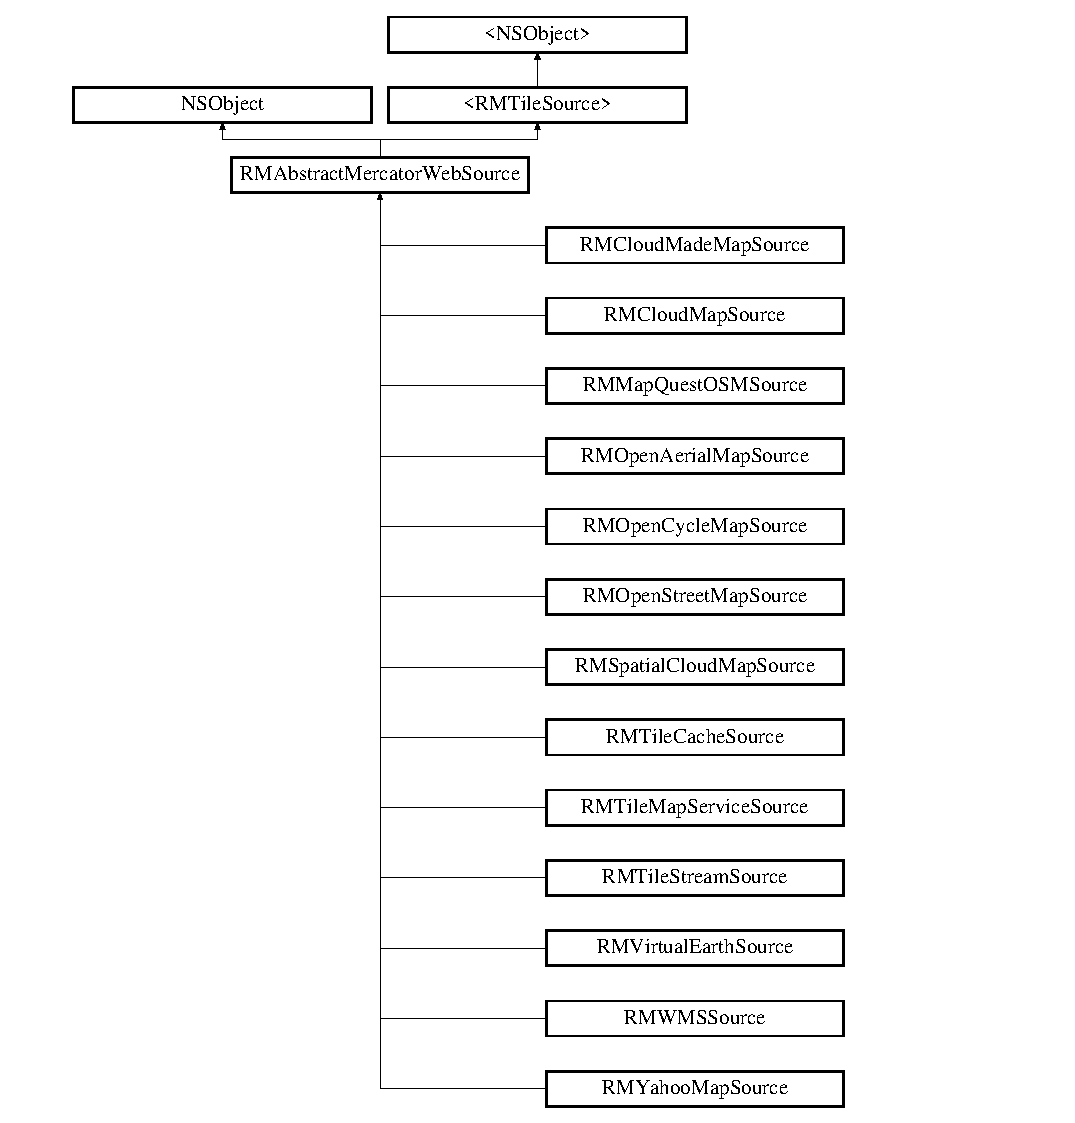
\includegraphics[height=12.000000cm]{interface_r_m_abstract_mercator_web_source}
\end{center}
\end{figure}
\subsection*{Instance Methods}
\begin{DoxyCompactItemize}
\item 
(void) -\/ \hyperlink{interface_r_m_abstract_mercator_web_source_a24301a2a9dd3c5839d0884251713c2e5}{dealloc}{\ttfamily  \mbox{[}implementation\mbox{]}}
\item 
(void) -\/ \hyperlink{interface_r_m_abstract_mercator_web_source_a560d3138401fbe5b7f8f7f358cf2e11b}{did\-Receive\-Memory\-Warning}{\ttfamily  \mbox{[}implementation\mbox{]}}
\item 
(id) -\/ \hyperlink{interface_r_m_abstract_mercator_web_source_a88bc1ea00a789381d77ae50e0eaec732}{init}
\item 
(\hyperlink{struct_r_m_spherical_trapezium}{R\-M\-Spherical\-Trapezium}) -\/ \hyperlink{interface_r_m_abstract_mercator_web_source_ae43425d7f2ade06fd2e3bdf34a8b083a}{latitude\-Longitude\-Bounding\-Box}
\item 
(N\-S\-String $\ast$) -\/ \hyperlink{interface_r_m_abstract_mercator_web_source_a77313c2d697428dd994a6e0cf07a256f}{long\-Attribution}
\item 
(N\-S\-String $\ast$) -\/ \hyperlink{interface_r_m_abstract_mercator_web_source_a9c1c86280c6fa05e4e82502822fcfd10}{long\-Description}
\item 
(float) -\/ \hyperlink{interface_r_m_abstract_mercator_web_source_a95d5287d9e661ba2e6c319fe9615c703}{max\-Zoom}
\item 
(id$<$ \hyperlink{protocol_r_m_mercator_to_tile_projection-p}{R\-M\-Mercator\-To\-Tile\-Projection} $>$) -\/ \hyperlink{interface_r_m_abstract_mercator_web_source_af48c0466d8040638076c5093f8b8234a}{mercator\-To\-Tile\-Projection}{\ttfamily  \mbox{[}implementation\mbox{]}}
\item 
(float) -\/ \hyperlink{interface_r_m_abstract_mercator_web_source_ae2767e8347256d6cc5eb88aec30fd97c}{min\-Zoom}
\item 
(void) -\/ \hyperlink{interface_r_m_abstract_mercator_web_source_ac370abc5403c594edcd8f6a59ab8907e}{network\-Operations\-Notification\-:}
\item 
(\hyperlink{interface_r_m_projection}{R\-M\-Projection} $\ast$) -\/ \hyperlink{interface_r_m_abstract_mercator_web_source_a7f9e2c871a2842dd854324fc173cd47f}{projection}{\ttfamily  \mbox{[}implementation\mbox{]}}
\item 
(void) -\/ \hyperlink{interface_r_m_abstract_mercator_web_source_a0d60c497c08e580f50acba5cb922fd97}{remove\-All\-Cached\-Images}{\ttfamily  \mbox{[}implementation\mbox{]}}
\begin{DoxyCompactList}\small\item\em clear all images from the in-\/memory and on-\/disk image caches \end{DoxyCompactList}\item 
(void) -\/ \hyperlink{interface_r_m_abstract_mercator_web_source_a3b6433a48a63999eb62cb3db63185d9c}{set\-Max\-Zoom\-:}{\ttfamily  \mbox{[}implementation\mbox{]}}
\item 
(void) -\/ \hyperlink{interface_r_m_abstract_mercator_web_source_ab30d98690abe95929a63f338635a898f}{set\-Min\-Zoom\-:}{\ttfamily  \mbox{[}implementation\mbox{]}}
\item 
(void) -\/ \hyperlink{interface_r_m_abstract_mercator_web_source_ad7f57c2c9ee2c43e1877195b56ac68f2}{set\-Tile\-Side\-Length\-:}
\item 
(N\-S\-String $\ast$) -\/ \hyperlink{interface_r_m_abstract_mercator_web_source_a6be24cea169d058b5eefd7572bedc366}{short\-Attribution}
\item 
(N\-S\-String $\ast$) -\/ \hyperlink{interface_r_m_abstract_mercator_web_source_a3e6c6ef18250ce14317373db9df1fc85}{short\-Name}
\item 
(N\-S\-String $\ast$) -\/ \hyperlink{interface_r_m_abstract_mercator_web_source_a5883e8ad44e66039acaa12c715a05154}{tile\-File\-:}{\ttfamily  \mbox{[}implementation\mbox{]}}
\item 
(\hyperlink{interface_r_m_tile_image}{R\-M\-Tile\-Image} $\ast$) -\/ \hyperlink{interface_r_m_abstract_mercator_web_source_a14e580ef6a285f9feedb8028a50b2b63}{tile\-Image\-:}{\ttfamily  \mbox{[}implementation\mbox{]}}
\item 
(N\-S\-String $\ast$) -\/ \hyperlink{interface_r_m_abstract_mercator_web_source_a00079a441d15a29bf5181e3672e9ba62}{tile\-Path}{\ttfamily  \mbox{[}implementation\mbox{]}}
\item 
(int) -\/ \hyperlink{interface_r_m_abstract_mercator_web_source_ae98cbd18cae13443ec8e71f7c850615b}{tile\-Side\-Length}
\item 
(N\-S\-String $\ast$) -\/ \hyperlink{interface_r_m_abstract_mercator_web_source_aba0294fce2e720adc6bf91180a90b28e}{tile\-U\-R\-L\-:}{\ttfamily  \mbox{[}implementation\mbox{]}}
\item 
(N\-S\-String $\ast$) -\/ \hyperlink{interface_r_m_abstract_mercator_web_source_acf45b84d8f39ef7fcc2a92a2e320a9a2}{unique\-Tilecache\-Key}{\ttfamily  \mbox{[}implementation\mbox{]}}
\end{DoxyCompactItemize}
\subsection*{Protected 属性}
\begin{DoxyCompactItemize}
\item 
B\-O\-O\-L \hyperlink{interface_r_m_abstract_mercator_web_source_ac05e057c8f0e7dc24790b673e136ce75}{network\-Operations}
\item 
\hyperlink{interface_r_m_fractal_tile_projection}{R\-M\-Fractal\-Tile\-Projection} $\ast$ \hyperlink{interface_r_m_abstract_mercator_web_source_abdb12e5197d9fb938a9d68bb0a9c9ae5}{tile\-Projection}
\end{DoxyCompactItemize}


\subsection{Method Documentation}
\hypertarget{interface_r_m_abstract_mercator_web_source_a24301a2a9dd3c5839d0884251713c2e5}{\index{R\-M\-Abstract\-Mercator\-Web\-Source@{R\-M\-Abstract\-Mercator\-Web\-Source}!dealloc@{dealloc}}
\index{dealloc@{dealloc}!RMAbstractMercatorWebSource@{R\-M\-Abstract\-Mercator\-Web\-Source}}
\subsubsection[{dealloc}]{\setlength{\rightskip}{0pt plus 5cm}-\/ (void) dealloc 
\begin{DoxyParamCaption}
{}
\end{DoxyParamCaption}
\hspace{0.3cm}{\ttfamily [implementation]}}}\label{interface_r_m_abstract_mercator_web_source_a24301a2a9dd3c5839d0884251713c2e5}


被 \hyperlink{interface_r_m_spatial_cloud_map_source_a6aeb222420a51b8b1a7f8cb13c2797e6}{R\-M\-Spatial\-Cloud\-Map\-Source}, \hyperlink{interface_r_m_w_m_s_source_a7df3f99e46ab5030506ddb7155e45911}{R\-M\-W\-M\-S\-Source} , 以及 \hyperlink{interface_r_m_tile_stream_source_a211ce6db8a319dab3d1089954b5d0f3a}{R\-M\-Tile\-Stream\-Source} 重载.



参考自 R\-M\-Tile\-Stream\-Source\-::dealloc, R\-M\-W\-M\-S\-Source\-::dealloc , 以及 R\-M\-Spatial\-Cloud\-Map\-Source\-::dealloc.

\hypertarget{interface_r_m_abstract_mercator_web_source_a560d3138401fbe5b7f8f7f358cf2e11b}{\index{R\-M\-Abstract\-Mercator\-Web\-Source@{R\-M\-Abstract\-Mercator\-Web\-Source}!did\-Receive\-Memory\-Warning@{did\-Receive\-Memory\-Warning}}
\index{did\-Receive\-Memory\-Warning@{did\-Receive\-Memory\-Warning}!RMAbstractMercatorWebSource@{R\-M\-Abstract\-Mercator\-Web\-Source}}
\subsubsection[{did\-Receive\-Memory\-Warning}]{\setlength{\rightskip}{0pt plus 5cm}-\/ (void) did\-Receive\-Memory\-Warning 
\begin{DoxyParamCaption}
{}
\end{DoxyParamCaption}
\hspace{0.3cm}{\ttfamily [implementation]}}}\label{interface_r_m_abstract_mercator_web_source_a560d3138401fbe5b7f8f7f358cf2e11b}


重载 \hyperlink{protocol_r_m_tile_source-p_a70eade96883de23124c3f86321685b52}{$<$\-R\-M\-Tile\-Source$>$} .

\hypertarget{interface_r_m_abstract_mercator_web_source_a88bc1ea00a789381d77ae50e0eaec732}{\index{R\-M\-Abstract\-Mercator\-Web\-Source@{R\-M\-Abstract\-Mercator\-Web\-Source}!init@{init}}
\index{init@{init}!RMAbstractMercatorWebSource@{R\-M\-Abstract\-Mercator\-Web\-Source}}
\subsubsection[{init}]{\setlength{\rightskip}{0pt plus 5cm}-\/ (id) init 
\begin{DoxyParamCaption}
{}
\end{DoxyParamCaption}
}}\label{interface_r_m_abstract_mercator_web_source_a88bc1ea00a789381d77ae50e0eaec732}


被 \hyperlink{interface_r_m_spatial_cloud_map_source_a69952598d6a2cc04c99a629a0df9588f}{R\-M\-Spatial\-Cloud\-Map\-Source}, \hyperlink{interface_r_m_w_m_s_source_af93c7233da63c1092768822cf25cb816}{R\-M\-W\-M\-S\-Source}, \hyperlink{interface_r_m_yahoo_map_source_ad3bb94f78cc1a8acb1f5a351c25976f2}{R\-M\-Yahoo\-Map\-Source}, \hyperlink{interface_r_m_virtual_earth_source_ac5adb7466431cc74785b23ccda89043a}{R\-M\-Virtual\-Earth\-Source}, \hyperlink{interface_r_m_tile_cache_source_a1991da8b9143df226620c9283792dab0}{R\-M\-Tile\-Cache\-Source}, \hyperlink{interface_r_m_map_quest_o_s_m_source_aecd8d0a7ca60bc224ee43f8ad933fb1b}{R\-M\-Map\-Quest\-O\-S\-M\-Source}, \hyperlink{interface_r_m_open_aerial_map_source_a05c9a3ffef1c399e854f0aaaa252924e}{R\-M\-Open\-Aerial\-Map\-Source}, \hyperlink{interface_r_m_open_cycle_map_source_a44641fcc78a286cb2deb35124e260165}{R\-M\-Open\-Cycle\-Map\-Source}, \hyperlink{interface_r_m_open_street_map_source_ad2c425f72e1d6342eb533a64426c1ecc}{R\-M\-Open\-Street\-Map\-Source}, \hyperlink{interface_r_m_cloud_made_map_source_ac1f36511f1261c96378989182fbdc724}{R\-M\-Cloud\-Made\-Map\-Source} , 以及 \hyperlink{interface_r_m_cloud_map_source_af878223b3719bd71f274050374cd7cda}{R\-M\-Cloud\-Map\-Source} 重载.



参考自 R\-M\-Spatial\-Cloud\-Map\-Source\-::init, R\-M\-Tile\-Map\-Service\-Source\-::init\-:unique\-Key\-:min\-Zoom\-:max\-Zoom\-: , 以及 R\-M\-Tile\-Stream\-Source\-::init\-With\-Info\-:.

\hypertarget{interface_r_m_abstract_mercator_web_source_ae43425d7f2ade06fd2e3bdf34a8b083a}{\index{R\-M\-Abstract\-Mercator\-Web\-Source@{R\-M\-Abstract\-Mercator\-Web\-Source}!latitude\-Longitude\-Bounding\-Box@{latitude\-Longitude\-Bounding\-Box}}
\index{latitude\-Longitude\-Bounding\-Box@{latitude\-Longitude\-Bounding\-Box}!RMAbstractMercatorWebSource@{R\-M\-Abstract\-Mercator\-Web\-Source}}
\subsubsection[{latitude\-Longitude\-Bounding\-Box}]{\setlength{\rightskip}{0pt plus 5cm}-\/ ({\bf R\-M\-Spherical\-Trapezium}) latitude\-Longitude\-Bounding\-Box 
\begin{DoxyParamCaption}
{}
\end{DoxyParamCaption}
}}\label{interface_r_m_abstract_mercator_web_source_ae43425d7f2ade06fd2e3bdf34a8b083a}


重载 \hyperlink{protocol_r_m_tile_source-p_a740893daebd1fe8e0a463e64a28816dd}{$<$\-R\-M\-Tile\-Source$>$} .



被 \hyperlink{interface_r_m_tile_stream_source_a483efb3bdcc1dad1a464506b94e39d78}{R\-M\-Tile\-Stream\-Source} 重载.

\hypertarget{interface_r_m_abstract_mercator_web_source_a77313c2d697428dd994a6e0cf07a256f}{\index{R\-M\-Abstract\-Mercator\-Web\-Source@{R\-M\-Abstract\-Mercator\-Web\-Source}!long\-Attribution@{long\-Attribution}}
\index{long\-Attribution@{long\-Attribution}!RMAbstractMercatorWebSource@{R\-M\-Abstract\-Mercator\-Web\-Source}}
\subsubsection[{long\-Attribution}]{\setlength{\rightskip}{0pt plus 5cm}-\/ (N\-S\-String $\ast$) long\-Attribution 
\begin{DoxyParamCaption}
{}
\end{DoxyParamCaption}
}}\label{interface_r_m_abstract_mercator_web_source_a77313c2d697428dd994a6e0cf07a256f}


重载 \hyperlink{protocol_r_m_tile_source-p_adff372c4c777906e56b90a61895d2ff4}{$<$\-R\-M\-Tile\-Source$>$} .



被 \hyperlink{interface_r_m_spatial_cloud_map_source_aca8e3d49e1f76041d359f4b3f23f455b}{R\-M\-Spatial\-Cloud\-Map\-Source}, \hyperlink{interface_r_m_yahoo_map_source_a3304e958de6f104c62db2cbba5003172}{R\-M\-Yahoo\-Map\-Source}, \hyperlink{interface_r_m_virtual_earth_source_aecb9344a0ea17a52805f4b275bf99f53}{R\-M\-Virtual\-Earth\-Source}, \hyperlink{interface_r_m_tile_cache_source_adc0c3fa292e6dd1fc59534be0d9eea26}{R\-M\-Tile\-Cache\-Source}, \hyperlink{interface_r_m_map_quest_o_s_m_source_a42722a15d1f14e114d2f4cd8de4010d6}{R\-M\-Map\-Quest\-O\-S\-M\-Source}, \hyperlink{interface_r_m_open_aerial_map_source_a3ee5ed718434f321be5ad57fe4c527b8}{R\-M\-Open\-Aerial\-Map\-Source}, \hyperlink{interface_r_m_open_cycle_map_source_af84dc5628aac3458972ab37a9364dd4d}{R\-M\-Open\-Cycle\-Map\-Source}, \hyperlink{interface_r_m_open_street_map_source_a932b3f4e2d2015eaadae1e5876f3fd14}{R\-M\-Open\-Street\-Map\-Source}, \hyperlink{interface_r_m_tile_stream_source_aa977502a8d80f3abcea6669c0cbb2fe7}{R\-M\-Tile\-Stream\-Source}, \hyperlink{interface_r_m_cloud_made_map_source_a591d36a1e1d2d5d5024a568339542b5e}{R\-M\-Cloud\-Made\-Map\-Source}, \hyperlink{interface_r_m_cloud_map_source_afc502c38dc65ff4ca970e7da5b39c5e1}{R\-M\-Cloud\-Map\-Source} , 以及 \hyperlink{interface_r_m_tile_map_service_source_af3e82c8c50ff4d3c6d8aa4940c0bbfd0}{R\-M\-Tile\-Map\-Service\-Source} 重载.

\hypertarget{interface_r_m_abstract_mercator_web_source_a9c1c86280c6fa05e4e82502822fcfd10}{\index{R\-M\-Abstract\-Mercator\-Web\-Source@{R\-M\-Abstract\-Mercator\-Web\-Source}!long\-Description@{long\-Description}}
\index{long\-Description@{long\-Description}!RMAbstractMercatorWebSource@{R\-M\-Abstract\-Mercator\-Web\-Source}}
\subsubsection[{long\-Description}]{\setlength{\rightskip}{0pt plus 5cm}-\/ (N\-S\-String $\ast$) long\-Description 
\begin{DoxyParamCaption}
{}
\end{DoxyParamCaption}
}}\label{interface_r_m_abstract_mercator_web_source_a9c1c86280c6fa05e4e82502822fcfd10}


重载 \hyperlink{protocol_r_m_tile_source-p_a1f9b03c3dac588a98b050afe3a71dcfa}{$<$\-R\-M\-Tile\-Source$>$} .



被 \hyperlink{interface_r_m_spatial_cloud_map_source_a92a59ece1bab8aae7c39fd8f26050930}{R\-M\-Spatial\-Cloud\-Map\-Source}, \hyperlink{interface_r_m_yahoo_map_source_ab368158d1562e382a66495d10778ced0}{R\-M\-Yahoo\-Map\-Source}, \hyperlink{interface_r_m_virtual_earth_source_aed0c86e17a29274bcd6749f9eaf8b0ba}{R\-M\-Virtual\-Earth\-Source}, \hyperlink{interface_r_m_tile_cache_source_a851d9a72047bd81351ec5dacb618c09f}{R\-M\-Tile\-Cache\-Source}, \hyperlink{interface_r_m_map_quest_o_s_m_source_ab56b7a7914bb63cbec37f5e0cf556efd}{R\-M\-Map\-Quest\-O\-S\-M\-Source}, \hyperlink{interface_r_m_open_aerial_map_source_a52f16e426510e04e68da57baa32e0a23}{R\-M\-Open\-Aerial\-Map\-Source}, \hyperlink{interface_r_m_open_cycle_map_source_a3d30e39f50df22cf3ddba68ae4eda864}{R\-M\-Open\-Cycle\-Map\-Source}, \hyperlink{interface_r_m_open_street_map_source_acf8470afa308a44db7eab70e1366c570}{R\-M\-Open\-Street\-Map\-Source}, \hyperlink{interface_r_m_tile_stream_source_a791cffd82b75f0c9853f2ed49aa635f4}{R\-M\-Tile\-Stream\-Source}, \hyperlink{interface_r_m_cloud_made_map_source_a0f04c8a09c3d1a9f25dcd4f45af2934b}{R\-M\-Cloud\-Made\-Map\-Source}, \hyperlink{interface_r_m_cloud_map_source_a4c0753b3fee1264ceca0dd2fd46af299}{R\-M\-Cloud\-Map\-Source} , 以及 \hyperlink{interface_r_m_tile_map_service_source_ad8821cb88d0e55e2f8cce4bb2a080209}{R\-M\-Tile\-Map\-Service\-Source} 重载.

\hypertarget{interface_r_m_abstract_mercator_web_source_a95d5287d9e661ba2e6c319fe9615c703}{\index{R\-M\-Abstract\-Mercator\-Web\-Source@{R\-M\-Abstract\-Mercator\-Web\-Source}!max\-Zoom@{max\-Zoom}}
\index{max\-Zoom@{max\-Zoom}!RMAbstractMercatorWebSource@{R\-M\-Abstract\-Mercator\-Web\-Source}}
\subsubsection[{max\-Zoom}]{\setlength{\rightskip}{0pt plus 5cm}-\/ (float) max\-Zoom 
\begin{DoxyParamCaption}
{}
\end{DoxyParamCaption}
}}\label{interface_r_m_abstract_mercator_web_source_a95d5287d9e661ba2e6c319fe9615c703}


重载 \hyperlink{protocol_r_m_tile_source-p_a7d1ecfedd45c8ac433f972f38e7ac9a4}{$<$\-R\-M\-Tile\-Source$>$} .



被 \hyperlink{interface_r_m_tile_stream_source_ad126cd46e17ef5ad95a6cf0533e17fe0}{R\-M\-Tile\-Stream\-Source} 重载.

\hypertarget{interface_r_m_abstract_mercator_web_source_af48c0466d8040638076c5093f8b8234a}{\index{R\-M\-Abstract\-Mercator\-Web\-Source@{R\-M\-Abstract\-Mercator\-Web\-Source}!mercator\-To\-Tile\-Projection@{mercator\-To\-Tile\-Projection}}
\index{mercator\-To\-Tile\-Projection@{mercator\-To\-Tile\-Projection}!RMAbstractMercatorWebSource@{R\-M\-Abstract\-Mercator\-Web\-Source}}
\subsubsection[{mercator\-To\-Tile\-Projection}]{\setlength{\rightskip}{0pt plus 5cm}-\/ (id$<$ {\bf R\-M\-Mercator\-To\-Tile\-Projection} $>$) mercator\-To\-Tile\-Projection 
\begin{DoxyParamCaption}
{}
\end{DoxyParamCaption}
\hspace{0.3cm}{\ttfamily [implementation]}}}\label{interface_r_m_abstract_mercator_web_source_af48c0466d8040638076c5093f8b8234a}


重载 \hyperlink{protocol_r_m_tile_source-p_a5086edf762a1756058c665c3a9b0d26f}{$<$\-R\-M\-Tile\-Source$>$} .

\hypertarget{interface_r_m_abstract_mercator_web_source_ae2767e8347256d6cc5eb88aec30fd97c}{\index{R\-M\-Abstract\-Mercator\-Web\-Source@{R\-M\-Abstract\-Mercator\-Web\-Source}!min\-Zoom@{min\-Zoom}}
\index{min\-Zoom@{min\-Zoom}!RMAbstractMercatorWebSource@{R\-M\-Abstract\-Mercator\-Web\-Source}}
\subsubsection[{min\-Zoom}]{\setlength{\rightskip}{0pt plus 5cm}-\/ (float) min\-Zoom 
\begin{DoxyParamCaption}
{}
\end{DoxyParamCaption}
}}\label{interface_r_m_abstract_mercator_web_source_ae2767e8347256d6cc5eb88aec30fd97c}


重载 \hyperlink{protocol_r_m_tile_source-p_a7cd043d2bc55eded244b4c5da41dd909}{$<$\-R\-M\-Tile\-Source$>$} .



被 \hyperlink{interface_r_m_tile_stream_source_a8a0c7a44fb2d194d2685c1f26187e6e5}{R\-M\-Tile\-Stream\-Source} 重载.

\hypertarget{interface_r_m_abstract_mercator_web_source_ac370abc5403c594edcd8f6a59ab8907e}{\index{R\-M\-Abstract\-Mercator\-Web\-Source@{R\-M\-Abstract\-Mercator\-Web\-Source}!network\-Operations\-Notification\-:@{network\-Operations\-Notification\-:}}
\index{network\-Operations\-Notification\-:@{network\-Operations\-Notification\-:}!RMAbstractMercatorWebSource@{R\-M\-Abstract\-Mercator\-Web\-Source}}
\subsubsection[{network\-Operations\-Notification\-:}]{\setlength{\rightskip}{0pt plus 5cm}-\/ (void) network\-Operations\-Notification\-: 
\begin{DoxyParamCaption}
\item[{(N\-S\-Notification$\ast$)}]{notification}
\end{DoxyParamCaption}
}}\label{interface_r_m_abstract_mercator_web_source_ac370abc5403c594edcd8f6a59ab8907e}
\hypertarget{interface_r_m_abstract_mercator_web_source_a7f9e2c871a2842dd854324fc173cd47f}{\index{R\-M\-Abstract\-Mercator\-Web\-Source@{R\-M\-Abstract\-Mercator\-Web\-Source}!projection@{projection}}
\index{projection@{projection}!RMAbstractMercatorWebSource@{R\-M\-Abstract\-Mercator\-Web\-Source}}
\subsubsection[{projection}]{\setlength{\rightskip}{0pt plus 5cm}-\/ ({\bf R\-M\-Projection} $\ast$) projection 
\begin{DoxyParamCaption}
{}
\end{DoxyParamCaption}
\hspace{0.3cm}{\ttfamily [implementation]}}}\label{interface_r_m_abstract_mercator_web_source_a7f9e2c871a2842dd854324fc173cd47f}


重载 \hyperlink{protocol_r_m_tile_source-p_a75c20205e72db39aa01943d8b6d8fc29}{$<$\-R\-M\-Tile\-Source$>$} .



参考自 init.

\hypertarget{interface_r_m_abstract_mercator_web_source_a0d60c497c08e580f50acba5cb922fd97}{\index{R\-M\-Abstract\-Mercator\-Web\-Source@{R\-M\-Abstract\-Mercator\-Web\-Source}!remove\-All\-Cached\-Images@{remove\-All\-Cached\-Images}}
\index{remove\-All\-Cached\-Images@{remove\-All\-Cached\-Images}!RMAbstractMercatorWebSource@{R\-M\-Abstract\-Mercator\-Web\-Source}}
\subsubsection[{remove\-All\-Cached\-Images}]{\setlength{\rightskip}{0pt plus 5cm}-\/ (void) remove\-All\-Cached\-Images 
\begin{DoxyParamCaption}
{}
\end{DoxyParamCaption}
\hspace{0.3cm}{\ttfamily [implementation]}}}\label{interface_r_m_abstract_mercator_web_source_a0d60c497c08e580f50acba5cb922fd97}


clear all images from the in-\/memory and on-\/disk image caches 

\begin{DoxyRefDesc}{Bug}
\item[\hyperlink{bug__bug000052}{Bug}]This method belongs on \hyperlink{interface_r_m_cached_tile_source}{R\-M\-Cached\-Tile\-Source}, not on \hyperlink{protocol_r_m_tile_source-p}{R\-M\-Tile\-Source}, because an \hyperlink{protocol_r_m_tile_source-p}{R\-M\-Tile\-Source} doesn't have a cache. \end{DoxyRefDesc}


重载 \hyperlink{protocol_r_m_tile_source-p_aa5c4555fb2500e5826d5558985d4ee3c}{$<$\-R\-M\-Tile\-Source$>$} .

\hypertarget{interface_r_m_abstract_mercator_web_source_a3b6433a48a63999eb62cb3db63185d9c}{\index{R\-M\-Abstract\-Mercator\-Web\-Source@{R\-M\-Abstract\-Mercator\-Web\-Source}!set\-Max\-Zoom\-:@{set\-Max\-Zoom\-:}}
\index{set\-Max\-Zoom\-:@{set\-Max\-Zoom\-:}!RMAbstractMercatorWebSource@{R\-M\-Abstract\-Mercator\-Web\-Source}}
\subsubsection[{set\-Max\-Zoom\-:}]{\setlength{\rightskip}{0pt plus 5cm}-\/ (void) set\-Max\-Zoom\-: 
\begin{DoxyParamCaption}
\item[{(N\-S\-U\-Integer)}]{a\-Max\-Zoom}
\end{DoxyParamCaption}
\hspace{0.3cm}{\ttfamily [implementation]}}}\label{interface_r_m_abstract_mercator_web_source_a3b6433a48a63999eb62cb3db63185d9c}


重载 \hyperlink{protocol_r_m_tile_source-p_afd2310f2b3b95e91de2ef530ee5d5122}{$<$\-R\-M\-Tile\-Source$>$} .



参考自 R\-M\-Cloud\-Map\-Source\-::init, R\-M\-Open\-Cycle\-Map\-Source\-::init, R\-M\-Open\-Street\-Map\-Source\-::init, R\-M\-Open\-Aerial\-Map\-Source\-::init, R\-M\-Map\-Quest\-O\-S\-M\-Source\-::init, R\-M\-W\-M\-S\-Source\-::init, R\-M\-Yahoo\-Map\-Source\-::init, R\-M\-Spatial\-Cloud\-Map\-Source\-::init, R\-M\-Tile\-Map\-Service\-Source\-::init\-:unique\-Key\-:min\-Zoom\-:max\-Zoom\-:, R\-M\-Virtual\-Earth\-Source\-::init\-With\-Aerial\-Theme\-Using\-Access\-Key\-:, R\-M\-Virtual\-Earth\-Source\-::init\-With\-Hybrid\-Theme\-Using\-Access\-Key\-: , 以及 R\-M\-Virtual\-Earth\-Source\-::init\-With\-Road\-Theme\-Using\-Access\-Key\-:.

\hypertarget{interface_r_m_abstract_mercator_web_source_ab30d98690abe95929a63f338635a898f}{\index{R\-M\-Abstract\-Mercator\-Web\-Source@{R\-M\-Abstract\-Mercator\-Web\-Source}!set\-Min\-Zoom\-:@{set\-Min\-Zoom\-:}}
\index{set\-Min\-Zoom\-:@{set\-Min\-Zoom\-:}!RMAbstractMercatorWebSource@{R\-M\-Abstract\-Mercator\-Web\-Source}}
\subsubsection[{set\-Min\-Zoom\-:}]{\setlength{\rightskip}{0pt plus 5cm}-\/ (void) set\-Min\-Zoom\-: 
\begin{DoxyParamCaption}
\item[{(N\-S\-U\-Integer)}]{a\-Min\-Zoom}
\end{DoxyParamCaption}
\hspace{0.3cm}{\ttfamily [implementation]}}}\label{interface_r_m_abstract_mercator_web_source_ab30d98690abe95929a63f338635a898f}


重载 \hyperlink{protocol_r_m_tile_source-p_ad8b2d3ab319784223970f215f6dd2f16}{$<$\-R\-M\-Tile\-Source$>$} .



参考自 R\-M\-Cloud\-Map\-Source\-::init, R\-M\-Open\-Cycle\-Map\-Source\-::init, R\-M\-Open\-Street\-Map\-Source\-::init, R\-M\-Open\-Aerial\-Map\-Source\-::init, R\-M\-Map\-Quest\-O\-S\-M\-Source\-::init, R\-M\-W\-M\-S\-Source\-::init, R\-M\-Yahoo\-Map\-Source\-::init, R\-M\-Spatial\-Cloud\-Map\-Source\-::init, R\-M\-Tile\-Map\-Service\-Source\-::init\-:unique\-Key\-:min\-Zoom\-:max\-Zoom\-:, R\-M\-Virtual\-Earth\-Source\-::init\-With\-Aerial\-Theme\-Using\-Access\-Key\-:, R\-M\-Virtual\-Earth\-Source\-::init\-With\-Hybrid\-Theme\-Using\-Access\-Key\-: , 以及 R\-M\-Virtual\-Earth\-Source\-::init\-With\-Road\-Theme\-Using\-Access\-Key\-:.

\hypertarget{interface_r_m_abstract_mercator_web_source_ad7f57c2c9ee2c43e1877195b56ac68f2}{\index{R\-M\-Abstract\-Mercator\-Web\-Source@{R\-M\-Abstract\-Mercator\-Web\-Source}!set\-Tile\-Side\-Length\-:@{set\-Tile\-Side\-Length\-:}}
\index{set\-Tile\-Side\-Length\-:@{set\-Tile\-Side\-Length\-:}!RMAbstractMercatorWebSource@{R\-M\-Abstract\-Mercator\-Web\-Source}}
\subsubsection[{set\-Tile\-Side\-Length\-:}]{\setlength{\rightskip}{0pt plus 5cm}-\/ (void) set\-Tile\-Side\-Length\-: 
\begin{DoxyParamCaption}
\item[{(N\-S\-U\-Integer)}]{a\-Tile\-Side\-Length}
\end{DoxyParamCaption}
}}\label{interface_r_m_abstract_mercator_web_source_ad7f57c2c9ee2c43e1877195b56ac68f2}


参考自 R\-M\-Cloud\-Made\-Map\-Source\-::init\-With\-Access\-Key\-:style\-Number\-:.

\hypertarget{interface_r_m_abstract_mercator_web_source_a6be24cea169d058b5eefd7572bedc366}{\index{R\-M\-Abstract\-Mercator\-Web\-Source@{R\-M\-Abstract\-Mercator\-Web\-Source}!short\-Attribution@{short\-Attribution}}
\index{short\-Attribution@{short\-Attribution}!RMAbstractMercatorWebSource@{R\-M\-Abstract\-Mercator\-Web\-Source}}
\subsubsection[{short\-Attribution}]{\setlength{\rightskip}{0pt plus 5cm}-\/ (N\-S\-String $\ast$) short\-Attribution 
\begin{DoxyParamCaption}
{}
\end{DoxyParamCaption}
}}\label{interface_r_m_abstract_mercator_web_source_a6be24cea169d058b5eefd7572bedc366}


重载 \hyperlink{protocol_r_m_tile_source-p_afd67cfacb812cd3216ef1309297e264d}{$<$\-R\-M\-Tile\-Source$>$} .



被 \hyperlink{interface_r_m_spatial_cloud_map_source_a54c0d41fc0dcf7a11dac1f9378098170}{R\-M\-Spatial\-Cloud\-Map\-Source}, \hyperlink{interface_r_m_yahoo_map_source_ae36d15de280147b8decd16d758874689}{R\-M\-Yahoo\-Map\-Source}, \hyperlink{interface_r_m_virtual_earth_source_a2571b1d3e25fa9ebacb40dca3d2bde8b}{R\-M\-Virtual\-Earth\-Source}, \hyperlink{interface_r_m_tile_cache_source_a700f4bcc6a9bbffb852d01eb425f8cfb}{R\-M\-Tile\-Cache\-Source}, \hyperlink{interface_r_m_map_quest_o_s_m_source_a14a58e74d28b38df3c93dfae7a7f6633}{R\-M\-Map\-Quest\-O\-S\-M\-Source}, \hyperlink{interface_r_m_open_aerial_map_source_ac20a79118d42831a77a162d4e42f3309}{R\-M\-Open\-Aerial\-Map\-Source}, \hyperlink{interface_r_m_open_cycle_map_source_a3c0c39e8ab0896390bd329e75e55860e}{R\-M\-Open\-Cycle\-Map\-Source}, \hyperlink{interface_r_m_open_street_map_source_a9ff8d53d553a5fd3e091a1dec5d720fe}{R\-M\-Open\-Street\-Map\-Source}, \hyperlink{interface_r_m_tile_stream_source_af29e760b684cfb520dbbd8f5f0f41686}{R\-M\-Tile\-Stream\-Source}, \hyperlink{interface_r_m_cloud_made_map_source_a24b31ad20954e02ffde188c4a008d2e8}{R\-M\-Cloud\-Made\-Map\-Source}, \hyperlink{interface_r_m_cloud_map_source_ada3be85455de2b8dae2032035d870f3e}{R\-M\-Cloud\-Map\-Source} , 以及 \hyperlink{interface_r_m_tile_map_service_source_ae40c5f9b838f852cb7c0943d0596c056}{R\-M\-Tile\-Map\-Service\-Source} 重载.



参考自 long\-Attribution.

\hypertarget{interface_r_m_abstract_mercator_web_source_a3e6c6ef18250ce14317373db9df1fc85}{\index{R\-M\-Abstract\-Mercator\-Web\-Source@{R\-M\-Abstract\-Mercator\-Web\-Source}!short\-Name@{short\-Name}}
\index{short\-Name@{short\-Name}!RMAbstractMercatorWebSource@{R\-M\-Abstract\-Mercator\-Web\-Source}}
\subsubsection[{short\-Name}]{\setlength{\rightskip}{0pt plus 5cm}-\/ (N\-S\-String $\ast$) short\-Name 
\begin{DoxyParamCaption}
{}
\end{DoxyParamCaption}
}}\label{interface_r_m_abstract_mercator_web_source_a3e6c6ef18250ce14317373db9df1fc85}


重载 \hyperlink{protocol_r_m_tile_source-p_ae0a98ebf46579f4c29d434322d25e64e}{$<$\-R\-M\-Tile\-Source$>$} .



被 \hyperlink{interface_r_m_spatial_cloud_map_source_a8979840374ba56ae17b72b53877071a8}{R\-M\-Spatial\-Cloud\-Map\-Source}, \hyperlink{interface_r_m_yahoo_map_source_ad41852333c9fbdba9664a56271ebf56e}{R\-M\-Yahoo\-Map\-Source}, \hyperlink{interface_r_m_virtual_earth_source_a3a9b18977a6a266312d7e4d79441b52f}{R\-M\-Virtual\-Earth\-Source}, \hyperlink{interface_r_m_tile_cache_source_a9d81b865c2a4ebb2757f2c1871fb6183}{R\-M\-Tile\-Cache\-Source}, \hyperlink{interface_r_m_map_quest_o_s_m_source_adb22b17b97840aa7bc2170e896b464d9}{R\-M\-Map\-Quest\-O\-S\-M\-Source}, \hyperlink{interface_r_m_open_aerial_map_source_aeee53f47d6b8e07c9db69a200e13738e}{R\-M\-Open\-Aerial\-Map\-Source}, \hyperlink{interface_r_m_open_cycle_map_source_ac9b00e3fbdde801fdda353681d05d838}{R\-M\-Open\-Cycle\-Map\-Source}, \hyperlink{interface_r_m_open_street_map_source_a2c36d88b3653099053eb46129a245a55}{R\-M\-Open\-Street\-Map\-Source}, \hyperlink{interface_r_m_tile_stream_source_a059871decc3a5ad1a72d70b691b343b7}{R\-M\-Tile\-Stream\-Source}, \hyperlink{interface_r_m_cloud_made_map_source_a5e956b126886325f16f34684d974262c}{R\-M\-Cloud\-Made\-Map\-Source}, \hyperlink{interface_r_m_cloud_map_source_ad968ed767e547a7f97753e0ec34dec63}{R\-M\-Cloud\-Map\-Source} , 以及 \hyperlink{interface_r_m_tile_map_service_source_ab6d355147c5578e213f8b822d7cc4753}{R\-M\-Tile\-Map\-Service\-Source} 重载.



参考自 long\-Description.

\hypertarget{interface_r_m_abstract_mercator_web_source_a5883e8ad44e66039acaa12c715a05154}{\index{R\-M\-Abstract\-Mercator\-Web\-Source@{R\-M\-Abstract\-Mercator\-Web\-Source}!tile\-File\-:@{tile\-File\-:}}
\index{tile\-File\-:@{tile\-File\-:}!RMAbstractMercatorWebSource@{R\-M\-Abstract\-Mercator\-Web\-Source}}
\subsubsection[{tile\-File\-:}]{\setlength{\rightskip}{0pt plus 5cm}-\/ (N\-S\-String $\ast$) tile\-File\-: 
\begin{DoxyParamCaption}
\item[{({\bf R\-M\-Tile})}]{tile}
\end{DoxyParamCaption}
\hspace{0.3cm}{\ttfamily [implementation]}}}\label{interface_r_m_abstract_mercator_web_source_a5883e8ad44e66039acaa12c715a05154}


重载 \hyperlink{protocol_r_m_tile_source-p_adc40bd2f04352819fc05e32d4209a2ca}{$<$\-R\-M\-Tile\-Source$>$} .



参考自 tile\-Image\-:.

\hypertarget{interface_r_m_abstract_mercator_web_source_a14e580ef6a285f9feedb8028a50b2b63}{\index{R\-M\-Abstract\-Mercator\-Web\-Source@{R\-M\-Abstract\-Mercator\-Web\-Source}!tile\-Image\-:@{tile\-Image\-:}}
\index{tile\-Image\-:@{tile\-Image\-:}!RMAbstractMercatorWebSource@{R\-M\-Abstract\-Mercator\-Web\-Source}}
\subsubsection[{tile\-Image\-:}]{\setlength{\rightskip}{0pt plus 5cm}-\/ ({\bf R\-M\-Tile\-Image} $\ast$) tile\-Image\-: 
\begin{DoxyParamCaption}
\item[{({\bf R\-M\-Tile})}]{tile}
\end{DoxyParamCaption}
\hspace{0.3cm}{\ttfamily [implementation]}}}\label{interface_r_m_abstract_mercator_web_source_a14e580ef6a285f9feedb8028a50b2b63}


重载 \hyperlink{protocol_r_m_tile_source-p_acf4ee01e3c1606d46a2ec8fe52b0d029}{$<$\-R\-M\-Tile\-Source$>$} .

\hypertarget{interface_r_m_abstract_mercator_web_source_a00079a441d15a29bf5181e3672e9ba62}{\index{R\-M\-Abstract\-Mercator\-Web\-Source@{R\-M\-Abstract\-Mercator\-Web\-Source}!tile\-Path@{tile\-Path}}
\index{tile\-Path@{tile\-Path}!RMAbstractMercatorWebSource@{R\-M\-Abstract\-Mercator\-Web\-Source}}
\subsubsection[{tile\-Path}]{\setlength{\rightskip}{0pt plus 5cm}-\/ (N\-S\-String $\ast$) tile\-Path 
\begin{DoxyParamCaption}
{}
\end{DoxyParamCaption}
\hspace{0.3cm}{\ttfamily [implementation]}}}\label{interface_r_m_abstract_mercator_web_source_a00079a441d15a29bf5181e3672e9ba62}


重载 \hyperlink{protocol_r_m_tile_source-p_ae9fc8d2cccf8a7ffce2a0f7837140b9b}{$<$\-R\-M\-Tile\-Source$>$} .

\hypertarget{interface_r_m_abstract_mercator_web_source_ae98cbd18cae13443ec8e71f7c850615b}{\index{R\-M\-Abstract\-Mercator\-Web\-Source@{R\-M\-Abstract\-Mercator\-Web\-Source}!tile\-Side\-Length@{tile\-Side\-Length}}
\index{tile\-Side\-Length@{tile\-Side\-Length}!RMAbstractMercatorWebSource@{R\-M\-Abstract\-Mercator\-Web\-Source}}
\subsubsection[{tile\-Side\-Length}]{\setlength{\rightskip}{0pt plus 5cm}-\/ (int) tile\-Side\-Length 
\begin{DoxyParamCaption}
{}
\end{DoxyParamCaption}
}}\label{interface_r_m_abstract_mercator_web_source_ae98cbd18cae13443ec8e71f7c850615b}
\hypertarget{interface_r_m_abstract_mercator_web_source_aba0294fce2e720adc6bf91180a90b28e}{\index{R\-M\-Abstract\-Mercator\-Web\-Source@{R\-M\-Abstract\-Mercator\-Web\-Source}!tile\-U\-R\-L\-:@{tile\-U\-R\-L\-:}}
\index{tile\-U\-R\-L\-:@{tile\-U\-R\-L\-:}!RMAbstractMercatorWebSource@{R\-M\-Abstract\-Mercator\-Web\-Source}}
\subsubsection[{tile\-U\-R\-L\-:}]{\setlength{\rightskip}{0pt plus 5cm}-\/ (N\-S\-String $\ast$) tile\-U\-R\-L\-: 
\begin{DoxyParamCaption}
\item[{({\bf R\-M\-Tile})}]{tile}
\end{DoxyParamCaption}
\hspace{0.3cm}{\ttfamily [implementation]}}}\label{interface_r_m_abstract_mercator_web_source_aba0294fce2e720adc6bf91180a90b28e}
\begin{DoxyRefDesc}{Bug}
\item[\hyperlink{bug__bug000001}{Bug}]magic string literals \end{DoxyRefDesc}


重载 \hyperlink{protocol_r_m_tile_source-p_af7ca2e2fb8e8cc4cb17433ffdc105230}{$<$\-R\-M\-Tile\-Source$>$} .



被 \hyperlink{interface_r_m_spatial_cloud_map_source_a8a29a9ae76880f3ceafb2b03fe2993be}{R\-M\-Spatial\-Cloud\-Map\-Source}, \hyperlink{interface_r_m_w_m_s_source_a87e46d1ac6e1a318323e4785b2c56d98}{R\-M\-W\-M\-S\-Source}, \hyperlink{interface_r_m_yahoo_map_source_a7e78f247de9a7ad3a6adcb1694d15380}{R\-M\-Yahoo\-Map\-Source}, \hyperlink{interface_r_m_virtual_earth_source_ae5d08adc0e9d810956f4f81a9fbf6681}{R\-M\-Virtual\-Earth\-Source}, \hyperlink{interface_r_m_tile_cache_source_a56bc01bcf515d76f547f84d79f9773e9}{R\-M\-Tile\-Cache\-Source}, \hyperlink{interface_r_m_map_quest_o_s_m_source_afb62c2d80e8f350ff3f1049f63e76b3b}{R\-M\-Map\-Quest\-O\-S\-M\-Source}, \hyperlink{interface_r_m_open_aerial_map_source_a4405601eb40cc53cf9d2f2875acc2be2}{R\-M\-Open\-Aerial\-Map\-Source}, \hyperlink{interface_r_m_open_cycle_map_source_a65f5b088a340d5b0e519a244f4f549fd}{R\-M\-Open\-Cycle\-Map\-Source}, \hyperlink{interface_r_m_open_street_map_source_a3d2b2c15f17ca1ab3d1862ffb1feb2e3}{R\-M\-Open\-Street\-Map\-Source}, \hyperlink{interface_r_m_tile_stream_source_ae4c4f099f3f2d43081accc1de9d2c5a8}{R\-M\-Tile\-Stream\-Source}, \hyperlink{interface_r_m_cloud_made_map_source_a25ff631fb042ace3eae48132f484a88e}{R\-M\-Cloud\-Made\-Map\-Source}, \hyperlink{interface_r_m_cloud_map_source_a13edb9f13639697b38732636d71688c1}{R\-M\-Cloud\-Map\-Source} , 以及 \hyperlink{interface_r_m_tile_map_service_source_a39aafcbb0907cfcca9df0f9708434f6b}{R\-M\-Tile\-Map\-Service\-Source} 重载.



参考自 tile\-Image\-:.

\hypertarget{interface_r_m_abstract_mercator_web_source_acf45b84d8f39ef7fcc2a92a2e320a9a2}{\index{R\-M\-Abstract\-Mercator\-Web\-Source@{R\-M\-Abstract\-Mercator\-Web\-Source}!unique\-Tilecache\-Key@{unique\-Tilecache\-Key}}
\index{unique\-Tilecache\-Key@{unique\-Tilecache\-Key}!RMAbstractMercatorWebSource@{R\-M\-Abstract\-Mercator\-Web\-Source}}
\subsubsection[{unique\-Tilecache\-Key}]{\setlength{\rightskip}{0pt plus 5cm}-\/ (N\-S\-String $\ast$) unique\-Tilecache\-Key 
\begin{DoxyParamCaption}
{}
\end{DoxyParamCaption}
\hspace{0.3cm}{\ttfamily [implementation]}}}\label{interface_r_m_abstract_mercator_web_source_acf45b84d8f39ef7fcc2a92a2e320a9a2}


重载 \hyperlink{protocol_r_m_tile_source-p_a1838a34e9341efe7c76252e131824261}{$<$\-R\-M\-Tile\-Source$>$} .



被 \hyperlink{interface_r_m_spatial_cloud_map_source_acb584cc15f37012168e4a81be5fb1a5d}{R\-M\-Spatial\-Cloud\-Map\-Source}, \hyperlink{interface_r_m_yahoo_map_source_aef91c1e282958b4c0f69e3ca885e28e9}{R\-M\-Yahoo\-Map\-Source}, \hyperlink{interface_r_m_virtual_earth_source_a8b7b461c2e4a8a89d51ca08e6d9d7628}{R\-M\-Virtual\-Earth\-Source}, \hyperlink{interface_r_m_tile_cache_source_a0fc37a76b0161717c4bf0de4a03d5fe0}{R\-M\-Tile\-Cache\-Source}, \hyperlink{interface_r_m_map_quest_o_s_m_source_ac5f1fbdc160544d60e9706b4e8e0c6a5}{R\-M\-Map\-Quest\-O\-S\-M\-Source}, \hyperlink{interface_r_m_open_aerial_map_source_a5da92a4a64ec3e3ecb36068b5264ca3f}{R\-M\-Open\-Aerial\-Map\-Source}, \hyperlink{interface_r_m_open_cycle_map_source_a8f454702038372b215a4cfabdce76022}{R\-M\-Open\-Cycle\-Map\-Source}, \hyperlink{interface_r_m_open_street_map_source_a6bf79a7fd62c28cb11979a7d4bdb65b9}{R\-M\-Open\-Street\-Map\-Source}, \hyperlink{interface_r_m_tile_stream_source_ab121a1455447ad90239e7f4ca78ce9a3}{R\-M\-Tile\-Stream\-Source}, \hyperlink{interface_r_m_cloud_made_map_source_aae477f125ad88298f778b14b079a7bbb}{R\-M\-Cloud\-Made\-Map\-Source}, \hyperlink{interface_r_m_cloud_map_source_a7c4d7bb98a9fee5864622a1c5e342dd8}{R\-M\-Cloud\-Map\-Source} , 以及 \hyperlink{interface_r_m_tile_map_service_source_a80f88caa0b6ea9310552e62714522348}{R\-M\-Tile\-Map\-Service\-Source} 重载.



\subsection{类成员变量说明}
\hypertarget{interface_r_m_abstract_mercator_web_source_ac05e057c8f0e7dc24790b673e136ce75}{\index{R\-M\-Abstract\-Mercator\-Web\-Source@{R\-M\-Abstract\-Mercator\-Web\-Source}!network\-Operations@{network\-Operations}}
\index{network\-Operations@{network\-Operations}!RMAbstractMercatorWebSource@{R\-M\-Abstract\-Mercator\-Web\-Source}}
\subsubsection[{network\-Operations}]{\setlength{\rightskip}{0pt plus 5cm}-\/ (B\-O\-O\-L) network\-Operations\hspace{0.3cm}{\ttfamily [protected]}}}\label{interface_r_m_abstract_mercator_web_source_ac05e057c8f0e7dc24790b673e136ce75}


参考自 init, network\-Operations\-Notification\-: , 以及 tile\-Image\-:.

\hypertarget{interface_r_m_abstract_mercator_web_source_abdb12e5197d9fb938a9d68bb0a9c9ae5}{\index{R\-M\-Abstract\-Mercator\-Web\-Source@{R\-M\-Abstract\-Mercator\-Web\-Source}!tile\-Projection@{tile\-Projection}}
\index{tile\-Projection@{tile\-Projection}!RMAbstractMercatorWebSource@{R\-M\-Abstract\-Mercator\-Web\-Source}}
\subsubsection[{tile\-Projection}]{\setlength{\rightskip}{0pt plus 5cm}-\/ ({\bf R\-M\-Fractal\-Tile\-Projection}$\ast$) tile\-Projection\hspace{0.3cm}{\ttfamily [protected]}}}\label{interface_r_m_abstract_mercator_web_source_abdb12e5197d9fb938a9d68bb0a9c9ae5}


参考自 dealloc, init, max\-Zoom, mercator\-To\-Tile\-Projection, min\-Zoom, set\-Max\-Zoom\-:, set\-Min\-Zoom\-:, set\-Tile\-Side\-Length\-:, tile\-Image\-: , 以及 tile\-Side\-Length.



该类的文档由以下文件生成\-:\begin{DoxyCompactItemize}
\item 
Map/\hyperlink{_r_m_abstract_mercator_web_source_8h}{R\-M\-Abstract\-Mercator\-Web\-Source.\-h}\item 
Map/\hyperlink{_r_m_abstract_mercator_web_source_8m}{R\-M\-Abstract\-Mercator\-Web\-Source.\-m}\end{DoxyCompactItemize}

\hypertarget{protocol_r_m_abstract_mercator_web_source-p}{\section{$<$R\-M\-Abstract\-Mercator\-Web\-Source$>$协议 参考}
\label{protocol_r_m_abstract_mercator_web_source-p}\index{$<$\-R\-M\-Abstract\-Mercator\-Web\-Source$>$@{$<$\-R\-M\-Abstract\-Mercator\-Web\-Source$>$}}
}


{\ttfamily \#import $<$R\-M\-Abstract\-Mercator\-Web\-Source.\-h$>$}

类 $<$R\-M\-Abstract\-Mercator\-Web\-Source$>$ 继承关系图\-:\begin{figure}[H]
\begin{center}
\leavevmode
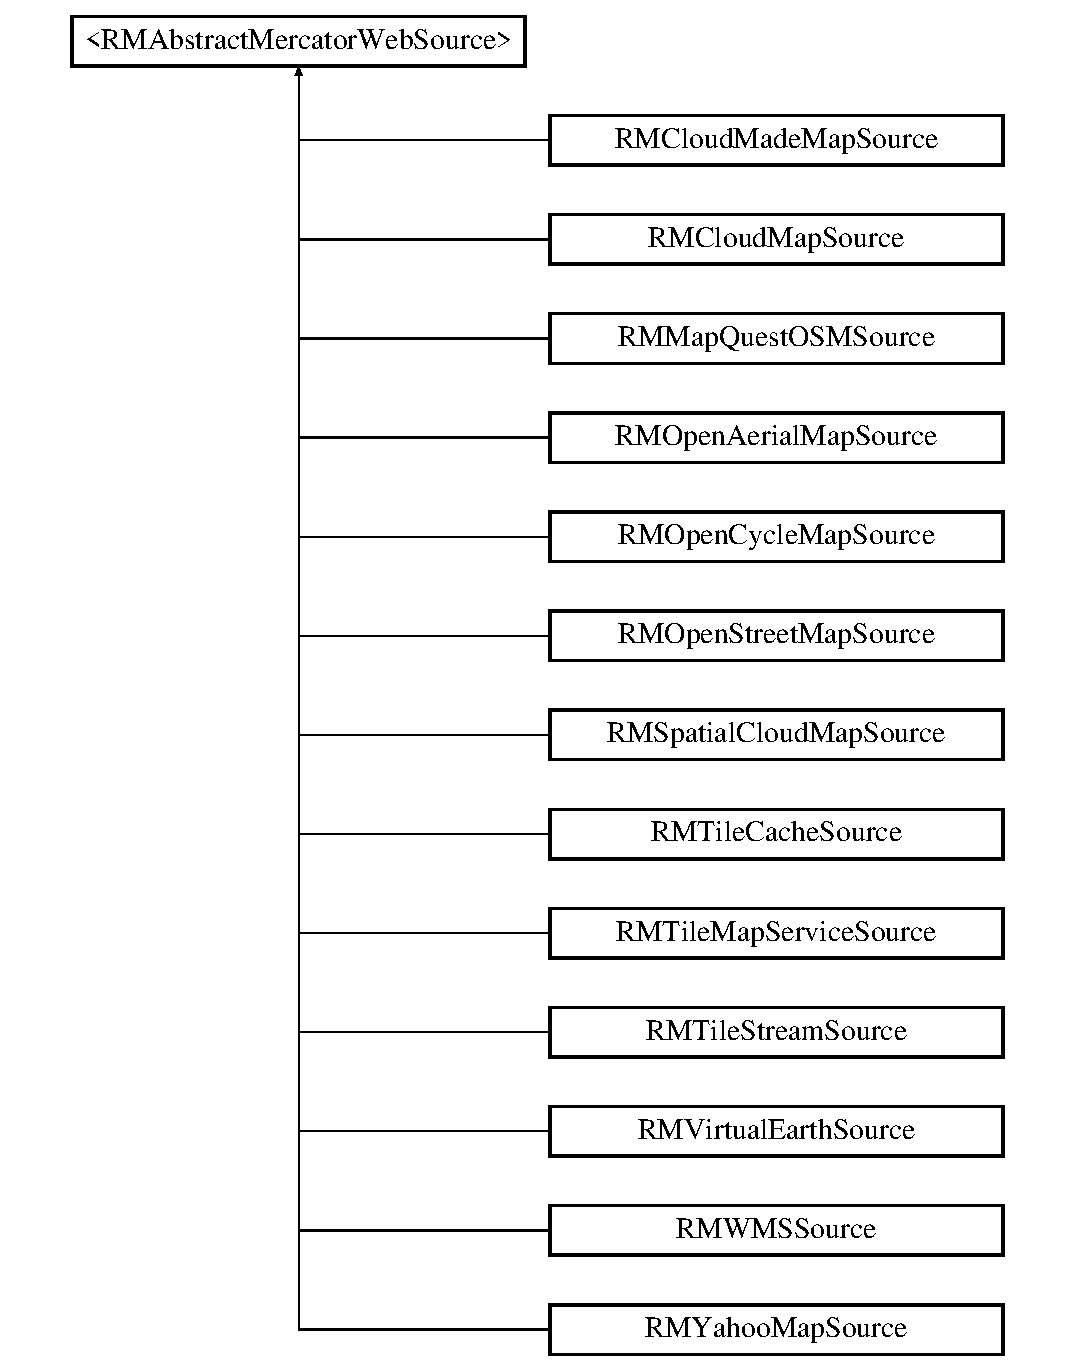
\includegraphics[height=12.000000cm]{protocol_r_m_abstract_mercator_web_source-p}
\end{center}
\end{figure}
\subsection*{Instance Methods}
\begin{DoxyCompactItemize}
\item 
(N\-S\-String $\ast$) -\/ \hyperlink{protocol_r_m_abstract_mercator_web_source-p_ae5c62f0fed7dcdfd78aa9582bdec9b4b}{tile\-U\-R\-L\-:}
\end{DoxyCompactItemize}


\subsection{Method Documentation}
\hypertarget{protocol_r_m_abstract_mercator_web_source-p_ae5c62f0fed7dcdfd78aa9582bdec9b4b}{\index{R\-M\-Abstract\-Mercator\-Web\-Source-\/p@{R\-M\-Abstract\-Mercator\-Web\-Source-\/p}!tile\-U\-R\-L\-:@{tile\-U\-R\-L\-:}}
\index{tile\-U\-R\-L\-:@{tile\-U\-R\-L\-:}!RMAbstractMercatorWebSource-p@{R\-M\-Abstract\-Mercator\-Web\-Source-\/p}}
\subsubsection[{tile\-U\-R\-L\-:}]{\setlength{\rightskip}{0pt plus 5cm}-\/ (N\-S\-String$\ast$) tile\-U\-R\-L\-: 
\begin{DoxyParamCaption}
\item[{({\bf R\-M\-Tile})}]{tile}
\end{DoxyParamCaption}
}}\label{protocol_r_m_abstract_mercator_web_source-p_ae5c62f0fed7dcdfd78aa9582bdec9b4b}


被 \hyperlink{interface_r_m_spatial_cloud_map_source_a8a29a9ae76880f3ceafb2b03fe2993be}{R\-M\-Spatial\-Cloud\-Map\-Source}, \hyperlink{interface_r_m_w_m_s_source_a87e46d1ac6e1a318323e4785b2c56d98}{R\-M\-W\-M\-S\-Source}, \hyperlink{interface_r_m_yahoo_map_source_a7e78f247de9a7ad3a6adcb1694d15380}{R\-M\-Yahoo\-Map\-Source}, \hyperlink{interface_r_m_virtual_earth_source_ae5d08adc0e9d810956f4f81a9fbf6681}{R\-M\-Virtual\-Earth\-Source}, \hyperlink{interface_r_m_tile_cache_source_a56bc01bcf515d76f547f84d79f9773e9}{R\-M\-Tile\-Cache\-Source}, \hyperlink{interface_r_m_map_quest_o_s_m_source_afb62c2d80e8f350ff3f1049f63e76b3b}{R\-M\-Map\-Quest\-O\-S\-M\-Source}, \hyperlink{interface_r_m_open_aerial_map_source_a4405601eb40cc53cf9d2f2875acc2be2}{R\-M\-Open\-Aerial\-Map\-Source}, \hyperlink{interface_r_m_open_cycle_map_source_a65f5b088a340d5b0e519a244f4f549fd}{R\-M\-Open\-Cycle\-Map\-Source}, \hyperlink{interface_r_m_open_street_map_source_a3d2b2c15f17ca1ab3d1862ffb1feb2e3}{R\-M\-Open\-Street\-Map\-Source}, \hyperlink{interface_r_m_tile_stream_source_ae4c4f099f3f2d43081accc1de9d2c5a8}{R\-M\-Tile\-Stream\-Source}, \hyperlink{interface_r_m_cloud_made_map_source_a25ff631fb042ace3eae48132f484a88e}{R\-M\-Cloud\-Made\-Map\-Source}, \hyperlink{interface_r_m_cloud_map_source_a13edb9f13639697b38732636d71688c1}{R\-M\-Cloud\-Map\-Source} , 以及 \hyperlink{interface_r_m_tile_map_service_source_a39aafcbb0907cfcca9df0f9708434f6b}{R\-M\-Tile\-Map\-Service\-Source} 重载.



该协议的文档由以下文件生成\-:\begin{DoxyCompactItemize}
\item 
Map/\hyperlink{_r_m_abstract_mercator_web_source_8h}{R\-M\-Abstract\-Mercator\-Web\-Source.\-h}\end{DoxyCompactItemize}

\hypertarget{interface_r_m_cached_tile_source}{\section{R\-M\-Cached\-Tile\-Source类 参考}
\label{interface_r_m_cached_tile_source}\index{R\-M\-Cached\-Tile\-Source@{R\-M\-Cached\-Tile\-Source}}
}


Simple wrapper around a tilesource which checks the image cache first.  




{\ttfamily \#import $<$R\-M\-Cached\-Tile\-Source.\-h$>$}

类 R\-M\-Cached\-Tile\-Source 继承关系图\-:\begin{figure}[H]
\begin{center}
\leavevmode
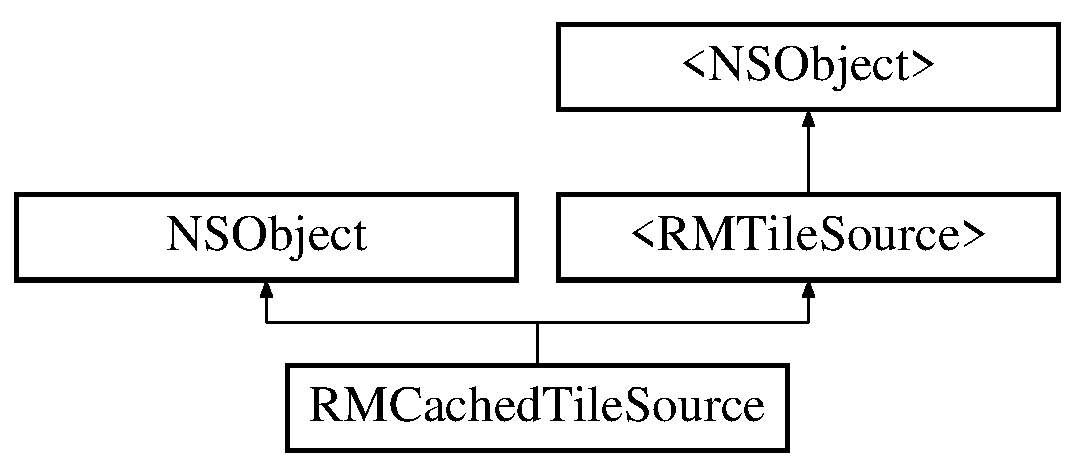
\includegraphics[height=3.000000cm]{interface_r_m_cached_tile_source}
\end{center}
\end{figure}
\subsection*{Instance Methods}
\begin{DoxyCompactItemize}
\item 
(void) -\/ \hyperlink{interface_r_m_cached_tile_source_acbfb800e18f97d6b0aa62a1e51c4a34d}{dealloc}{\ttfamily  \mbox{[}implementation\mbox{]}}
\item 
(void) -\/ \hyperlink{interface_r_m_cached_tile_source_a2a17377fc15beaea12ef271cc0c7910b}{did\-Receive\-Memory\-Warning}
\item 
(id) -\/ \hyperlink{interface_r_m_cached_tile_source_a67899f6340f78fad6ec0e9fec134165d}{init\-With\-Source\-:}
\item 
(\hyperlink{struct_r_m_spherical_trapezium}{R\-M\-Spherical\-Trapezium}) -\/ \hyperlink{interface_r_m_cached_tile_source_a18bb86664692698478705d78ff100bf1}{latitude\-Longitude\-Bounding\-Box}{\ttfamily  \mbox{[}implementation\mbox{]}}
\item 
(N\-S\-String $\ast$) -\/ \hyperlink{interface_r_m_cached_tile_source_a09c61195fbb3b3b41d025b092c830455}{legend}
\item 
(N\-S\-String $\ast$) -\/ \hyperlink{interface_r_m_cached_tile_source_ad9da1c346c64d04310f4f1c3a1ec43e7}{long\-Attribution}
\item 
(N\-S\-String $\ast$) -\/ \hyperlink{interface_r_m_cached_tile_source_ad9402dc9453199fcb71127d0ff137ab8}{long\-Description}
\item 
(float) -\/ \hyperlink{interface_r_m_cached_tile_source_a0946e8601ca057c889341e6238ea12b8}{max\-Zoom}{\ttfamily  \mbox{[}implementation\mbox{]}}
\item 
(id$<$ \hyperlink{protocol_r_m_mercator_to_tile_projection-p}{R\-M\-Mercator\-To\-Tile\-Projection} $>$) -\/ \hyperlink{interface_r_m_cached_tile_source_a611ec223df3c49d9ccb6b29670e7c65a}{mercator\-To\-Tile\-Projection}{\ttfamily  \mbox{[}implementation\mbox{]}}
\item 
(float) -\/ \hyperlink{interface_r_m_cached_tile_source_adf9a9a4074baf19c89210b1fca0ed32f}{min\-Zoom}{\ttfamily  \mbox{[}implementation\mbox{]}}
\item 
(\hyperlink{interface_r_m_projection}{R\-M\-Projection} $\ast$) -\/ \hyperlink{interface_r_m_cached_tile_source_a7fd23ce549a314c91034127da0ce5c8a}{projection}{\ttfamily  \mbox{[}implementation\mbox{]}}
\item 
(void) -\/ \hyperlink{interface_r_m_cached_tile_source_a07c40b88ceb0b2d8fed56f35ea52e82a}{remove\-All\-Cached\-Images}{\ttfamily  \mbox{[}implementation\mbox{]}}
\begin{DoxyCompactList}\small\item\em clear all images from the in-\/memory and on-\/disk image caches \end{DoxyCompactList}\item 
(void) -\/ \hyperlink{interface_r_m_cached_tile_source_abfc94f15a69698f3ff8c127a66bda7a4}{set\-Max\-Zoom\-:}{\ttfamily  \mbox{[}implementation\mbox{]}}
\item 
(void) -\/ \hyperlink{interface_r_m_cached_tile_source_af62c9fa10f55febeef1054ae644cc045}{set\-Min\-Zoom\-:}{\ttfamily  \mbox{[}implementation\mbox{]}}
\item 
(N\-S\-String $\ast$) -\/ \hyperlink{interface_r_m_cached_tile_source_addd642460ef82b300d67d60813d6338d}{short\-Attribution}
\item 
(N\-S\-String $\ast$) -\/ \hyperlink{interface_r_m_cached_tile_source_a70953c71ca922e6dd6093a94723efbb5}{short\-Name}
\item 
(N\-S\-String $\ast$) -\/ \hyperlink{interface_r_m_cached_tile_source_a4a4b44c6e1899ad11e9a72e21502861a}{tile\-File\-:}
\item 
(\hyperlink{interface_r_m_tile_image}{R\-M\-Tile\-Image} $\ast$) -\/ \hyperlink{interface_r_m_cached_tile_source_a21743e9d45e9ce2accf27dd098e1b2f0}{tile\-Image\-:}{\ttfamily  \mbox{[}implementation\mbox{]}}
\item 
(N\-S\-String $\ast$) -\/ \hyperlink{interface_r_m_cached_tile_source_a49619cfba67b331c19bdab55cfe3475f}{tile\-Path}
\item 
(N\-S\-String $\ast$) -\/ \hyperlink{interface_r_m_cached_tile_source_a96037f61390856cb9dda7e955ff1f551}{tile\-U\-R\-L\-:}
\item 
(id$<$ \hyperlink{protocol_r_m_tile_source-p}{R\-M\-Tile\-Source} $>$) -\/ \hyperlink{interface_r_m_cached_tile_source_a07fd06ac405d532aba3653e965b279a1}{underlying\-Tile\-Source}
\item 
(N\-S\-String $\ast$) -\/ \hyperlink{interface_r_m_cached_tile_source_aa6226fe9784e2f6b47b45ea24d7c062f}{unique\-Tilecache\-Key}{\ttfamily  \mbox{[}implementation\mbox{]}}
\end{DoxyCompactItemize}
\subsection*{Class Methods}
\begin{DoxyCompactItemize}
\item 
(\hyperlink{interface_r_m_cached_tile_source}{R\-M\-Cached\-Tile\-Source} $\ast$) + \hyperlink{interface_r_m_cached_tile_source_a3ae5adfa3d611c7fef0080813e9cf766}{cached\-Tile\-Source\-With\-Source\-:}
\begin{DoxyCompactList}\small\item\em Bleah ugly name. \end{DoxyCompactList}\end{DoxyCompactItemize}
\subsection*{Protected 属性}
\begin{DoxyCompactItemize}
\item 
\hyperlink{interface_r_m_tile_cache}{R\-M\-Tile\-Cache} $\ast$ \hyperlink{interface_r_m_cached_tile_source_a6bfbfd532bdc05e0ea95a67db19574fd}{cache}
\item 
id$<$ \hyperlink{protocol_r_m_tile_source-p}{R\-M\-Tile\-Source} $>$ \hyperlink{interface_r_m_cached_tile_source_a1d18d0de8f4c6bfd360c79e211a07ca9}{tile\-Source}
\end{DoxyCompactItemize}


\subsection{详细描述}
Simple wrapper around a tilesource which checks the image cache first. 

\subsection{Method Documentation}
\hypertarget{interface_r_m_cached_tile_source_a3ae5adfa3d611c7fef0080813e9cf766}{\index{R\-M\-Cached\-Tile\-Source@{R\-M\-Cached\-Tile\-Source}!cached\-Tile\-Source\-With\-Source\-:@{cached\-Tile\-Source\-With\-Source\-:}}
\index{cached\-Tile\-Source\-With\-Source\-:@{cached\-Tile\-Source\-With\-Source\-:}!RMCachedTileSource@{R\-M\-Cached\-Tile\-Source}}
\subsubsection[{cached\-Tile\-Source\-With\-Source\-:}]{\setlength{\rightskip}{0pt plus 5cm}+ ({\bf R\-M\-Cached\-Tile\-Source} $\ast$) cached\-Tile\-Source\-With\-Source\-: 
\begin{DoxyParamCaption}
\item[{(id$<${\bf R\-M\-Tile\-Source}$>$)}]{source}
\end{DoxyParamCaption}
}}\label{interface_r_m_cached_tile_source_a3ae5adfa3d611c7fef0080813e9cf766}


Bleah ugly name. 



参考自 R\-M\-Map\-Contents\-::set\-Tile\-Source\-:.

\hypertarget{interface_r_m_cached_tile_source_acbfb800e18f97d6b0aa62a1e51c4a34d}{\index{R\-M\-Cached\-Tile\-Source@{R\-M\-Cached\-Tile\-Source}!dealloc@{dealloc}}
\index{dealloc@{dealloc}!RMCachedTileSource@{R\-M\-Cached\-Tile\-Source}}
\subsubsection[{dealloc}]{\setlength{\rightskip}{0pt plus 5cm}-\/ (void) dealloc 
\begin{DoxyParamCaption}
{}
\end{DoxyParamCaption}
\hspace{0.3cm}{\ttfamily [implementation]}}}\label{interface_r_m_cached_tile_source_acbfb800e18f97d6b0aa62a1e51c4a34d}
\hypertarget{interface_r_m_cached_tile_source_a2a17377fc15beaea12ef271cc0c7910b}{\index{R\-M\-Cached\-Tile\-Source@{R\-M\-Cached\-Tile\-Source}!did\-Receive\-Memory\-Warning@{did\-Receive\-Memory\-Warning}}
\index{did\-Receive\-Memory\-Warning@{did\-Receive\-Memory\-Warning}!RMCachedTileSource@{R\-M\-Cached\-Tile\-Source}}
\subsubsection[{did\-Receive\-Memory\-Warning}]{\setlength{\rightskip}{0pt plus 5cm}-\/ (void) did\-Receive\-Memory\-Warning 
\begin{DoxyParamCaption}
{}
\end{DoxyParamCaption}
}}\label{interface_r_m_cached_tile_source_a2a17377fc15beaea12ef271cc0c7910b}


重载 \hyperlink{protocol_r_m_tile_source-p_a70eade96883de23124c3f86321685b52}{$<$\-R\-M\-Tile\-Source$>$} .

\hypertarget{interface_r_m_cached_tile_source_a67899f6340f78fad6ec0e9fec134165d}{\index{R\-M\-Cached\-Tile\-Source@{R\-M\-Cached\-Tile\-Source}!init\-With\-Source\-:@{init\-With\-Source\-:}}
\index{init\-With\-Source\-:@{init\-With\-Source\-:}!RMCachedTileSource@{R\-M\-Cached\-Tile\-Source}}
\subsubsection[{init\-With\-Source\-:}]{\setlength{\rightskip}{0pt plus 5cm}-\/ (id) init\-With\-Source\-: 
\begin{DoxyParamCaption}
\item[{(id$<${\bf R\-M\-Tile\-Source}$>$)}]{source}
\end{DoxyParamCaption}
}}\label{interface_r_m_cached_tile_source_a67899f6340f78fad6ec0e9fec134165d}
\hypertarget{interface_r_m_cached_tile_source_a18bb86664692698478705d78ff100bf1}{\index{R\-M\-Cached\-Tile\-Source@{R\-M\-Cached\-Tile\-Source}!latitude\-Longitude\-Bounding\-Box@{latitude\-Longitude\-Bounding\-Box}}
\index{latitude\-Longitude\-Bounding\-Box@{latitude\-Longitude\-Bounding\-Box}!RMCachedTileSource@{R\-M\-Cached\-Tile\-Source}}
\subsubsection[{latitude\-Longitude\-Bounding\-Box}]{\setlength{\rightskip}{0pt plus 5cm}-\/ ({\bf R\-M\-Spherical\-Trapezium}) latitude\-Longitude\-Bounding\-Box 
\begin{DoxyParamCaption}
{}
\end{DoxyParamCaption}
\hspace{0.3cm}{\ttfamily [implementation]}}}\label{interface_r_m_cached_tile_source_a18bb86664692698478705d78ff100bf1}


重载 \hyperlink{protocol_r_m_tile_source-p_a740893daebd1fe8e0a463e64a28816dd}{$<$\-R\-M\-Tile\-Source$>$} .

\hypertarget{interface_r_m_cached_tile_source_a09c61195fbb3b3b41d025b092c830455}{\index{R\-M\-Cached\-Tile\-Source@{R\-M\-Cached\-Tile\-Source}!legend@{legend}}
\index{legend@{legend}!RMCachedTileSource@{R\-M\-Cached\-Tile\-Source}}
\subsubsection[{legend}]{\setlength{\rightskip}{0pt plus 5cm}-\/ (N\-S\-String $\ast$) legend 
\begin{DoxyParamCaption}
{}
\end{DoxyParamCaption}
}}\label{interface_r_m_cached_tile_source_a09c61195fbb3b3b41d025b092c830455}


Provided by category \hyperlink{category_r_m_cached_tile_source_07_r_m_tile_stream_source_extensions_08_a09c61195fbb3b3b41d025b092c830455}{R\-M\-Cached\-Tile\-Source(\-R\-M\-Tile\-Stream\-Source\-Extensions)}.

\hypertarget{interface_r_m_cached_tile_source_ad9da1c346c64d04310f4f1c3a1ec43e7}{\index{R\-M\-Cached\-Tile\-Source@{R\-M\-Cached\-Tile\-Source}!long\-Attribution@{long\-Attribution}}
\index{long\-Attribution@{long\-Attribution}!RMCachedTileSource@{R\-M\-Cached\-Tile\-Source}}
\subsubsection[{long\-Attribution}]{\setlength{\rightskip}{0pt plus 5cm}-\/ (N\-S\-String $\ast$) long\-Attribution 
\begin{DoxyParamCaption}
{}
\end{DoxyParamCaption}
}}\label{interface_r_m_cached_tile_source_ad9da1c346c64d04310f4f1c3a1ec43e7}


重载 \hyperlink{protocol_r_m_tile_source-p_adff372c4c777906e56b90a61895d2ff4}{$<$\-R\-M\-Tile\-Source$>$} .

\hypertarget{interface_r_m_cached_tile_source_ad9402dc9453199fcb71127d0ff137ab8}{\index{R\-M\-Cached\-Tile\-Source@{R\-M\-Cached\-Tile\-Source}!long\-Description@{long\-Description}}
\index{long\-Description@{long\-Description}!RMCachedTileSource@{R\-M\-Cached\-Tile\-Source}}
\subsubsection[{long\-Description}]{\setlength{\rightskip}{0pt plus 5cm}-\/ (N\-S\-String $\ast$) long\-Description 
\begin{DoxyParamCaption}
{}
\end{DoxyParamCaption}
}}\label{interface_r_m_cached_tile_source_ad9402dc9453199fcb71127d0ff137ab8}


重载 \hyperlink{protocol_r_m_tile_source-p_a1f9b03c3dac588a98b050afe3a71dcfa}{$<$\-R\-M\-Tile\-Source$>$} .

\hypertarget{interface_r_m_cached_tile_source_a0946e8601ca057c889341e6238ea12b8}{\index{R\-M\-Cached\-Tile\-Source@{R\-M\-Cached\-Tile\-Source}!max\-Zoom@{max\-Zoom}}
\index{max\-Zoom@{max\-Zoom}!RMCachedTileSource@{R\-M\-Cached\-Tile\-Source}}
\subsubsection[{max\-Zoom}]{\setlength{\rightskip}{0pt plus 5cm}-\/ (float) max\-Zoom 
\begin{DoxyParamCaption}
{}
\end{DoxyParamCaption}
\hspace{0.3cm}{\ttfamily [implementation]}}}\label{interface_r_m_cached_tile_source_a0946e8601ca057c889341e6238ea12b8}


重载 \hyperlink{protocol_r_m_tile_source-p_a7d1ecfedd45c8ac433f972f38e7ac9a4}{$<$\-R\-M\-Tile\-Source$>$} .

\hypertarget{interface_r_m_cached_tile_source_a611ec223df3c49d9ccb6b29670e7c65a}{\index{R\-M\-Cached\-Tile\-Source@{R\-M\-Cached\-Tile\-Source}!mercator\-To\-Tile\-Projection@{mercator\-To\-Tile\-Projection}}
\index{mercator\-To\-Tile\-Projection@{mercator\-To\-Tile\-Projection}!RMCachedTileSource@{R\-M\-Cached\-Tile\-Source}}
\subsubsection[{mercator\-To\-Tile\-Projection}]{\setlength{\rightskip}{0pt plus 5cm}-\/ (id$<$ {\bf R\-M\-Mercator\-To\-Tile\-Projection} $>$) mercator\-To\-Tile\-Projection 
\begin{DoxyParamCaption}
{}
\end{DoxyParamCaption}
\hspace{0.3cm}{\ttfamily [implementation]}}}\label{interface_r_m_cached_tile_source_a611ec223df3c49d9ccb6b29670e7c65a}


重载 \hyperlink{protocol_r_m_tile_source-p_a5086edf762a1756058c665c3a9b0d26f}{$<$\-R\-M\-Tile\-Source$>$} .

\hypertarget{interface_r_m_cached_tile_source_adf9a9a4074baf19c89210b1fca0ed32f}{\index{R\-M\-Cached\-Tile\-Source@{R\-M\-Cached\-Tile\-Source}!min\-Zoom@{min\-Zoom}}
\index{min\-Zoom@{min\-Zoom}!RMCachedTileSource@{R\-M\-Cached\-Tile\-Source}}
\subsubsection[{min\-Zoom}]{\setlength{\rightskip}{0pt plus 5cm}-\/ (float) min\-Zoom 
\begin{DoxyParamCaption}
{}
\end{DoxyParamCaption}
\hspace{0.3cm}{\ttfamily [implementation]}}}\label{interface_r_m_cached_tile_source_adf9a9a4074baf19c89210b1fca0ed32f}


重载 \hyperlink{protocol_r_m_tile_source-p_a7cd043d2bc55eded244b4c5da41dd909}{$<$\-R\-M\-Tile\-Source$>$} .

\hypertarget{interface_r_m_cached_tile_source_a7fd23ce549a314c91034127da0ce5c8a}{\index{R\-M\-Cached\-Tile\-Source@{R\-M\-Cached\-Tile\-Source}!projection@{projection}}
\index{projection@{projection}!RMCachedTileSource@{R\-M\-Cached\-Tile\-Source}}
\subsubsection[{projection}]{\setlength{\rightskip}{0pt plus 5cm}-\/ ({\bf R\-M\-Projection} $\ast$) projection 
\begin{DoxyParamCaption}
{}
\end{DoxyParamCaption}
\hspace{0.3cm}{\ttfamily [implementation]}}}\label{interface_r_m_cached_tile_source_a7fd23ce549a314c91034127da0ce5c8a}


重载 \hyperlink{protocol_r_m_tile_source-p_a75c20205e72db39aa01943d8b6d8fc29}{$<$\-R\-M\-Tile\-Source$>$} .

\hypertarget{interface_r_m_cached_tile_source_a07c40b88ceb0b2d8fed56f35ea52e82a}{\index{R\-M\-Cached\-Tile\-Source@{R\-M\-Cached\-Tile\-Source}!remove\-All\-Cached\-Images@{remove\-All\-Cached\-Images}}
\index{remove\-All\-Cached\-Images@{remove\-All\-Cached\-Images}!RMCachedTileSource@{R\-M\-Cached\-Tile\-Source}}
\subsubsection[{remove\-All\-Cached\-Images}]{\setlength{\rightskip}{0pt plus 5cm}-\/ (void) remove\-All\-Cached\-Images 
\begin{DoxyParamCaption}
{}
\end{DoxyParamCaption}
\hspace{0.3cm}{\ttfamily [implementation]}}}\label{interface_r_m_cached_tile_source_a07c40b88ceb0b2d8fed56f35ea52e82a}


clear all images from the in-\/memory and on-\/disk image caches 

\begin{DoxyRefDesc}{Bug}
\item[\hyperlink{bug__bug000052}{Bug}]This method belongs on \hyperlink{interface_r_m_cached_tile_source}{R\-M\-Cached\-Tile\-Source}, not on \hyperlink{protocol_r_m_tile_source-p}{R\-M\-Tile\-Source}, because an \hyperlink{protocol_r_m_tile_source-p}{R\-M\-Tile\-Source} doesn't have a cache. \end{DoxyRefDesc}


重载 \hyperlink{protocol_r_m_tile_source-p_aa5c4555fb2500e5826d5558985d4ee3c}{$<$\-R\-M\-Tile\-Source$>$} .

\hypertarget{interface_r_m_cached_tile_source_abfc94f15a69698f3ff8c127a66bda7a4}{\index{R\-M\-Cached\-Tile\-Source@{R\-M\-Cached\-Tile\-Source}!set\-Max\-Zoom\-:@{set\-Max\-Zoom\-:}}
\index{set\-Max\-Zoom\-:@{set\-Max\-Zoom\-:}!RMCachedTileSource@{R\-M\-Cached\-Tile\-Source}}
\subsubsection[{set\-Max\-Zoom\-:}]{\setlength{\rightskip}{0pt plus 5cm}-\/ (void) set\-Max\-Zoom\-: 
\begin{DoxyParamCaption}
\item[{(N\-S\-U\-Integer)}]{a\-Max\-Zoom}
\end{DoxyParamCaption}
\hspace{0.3cm}{\ttfamily [implementation]}}}\label{interface_r_m_cached_tile_source_abfc94f15a69698f3ff8c127a66bda7a4}


重载 \hyperlink{protocol_r_m_tile_source-p_afd2310f2b3b95e91de2ef530ee5d5122}{$<$\-R\-M\-Tile\-Source$>$} .

\hypertarget{interface_r_m_cached_tile_source_af62c9fa10f55febeef1054ae644cc045}{\index{R\-M\-Cached\-Tile\-Source@{R\-M\-Cached\-Tile\-Source}!set\-Min\-Zoom\-:@{set\-Min\-Zoom\-:}}
\index{set\-Min\-Zoom\-:@{set\-Min\-Zoom\-:}!RMCachedTileSource@{R\-M\-Cached\-Tile\-Source}}
\subsubsection[{set\-Min\-Zoom\-:}]{\setlength{\rightskip}{0pt plus 5cm}-\/ (void) set\-Min\-Zoom\-: 
\begin{DoxyParamCaption}
\item[{(N\-S\-U\-Integer)}]{a\-Min\-Zoom}
\end{DoxyParamCaption}
\hspace{0.3cm}{\ttfamily [implementation]}}}\label{interface_r_m_cached_tile_source_af62c9fa10f55febeef1054ae644cc045}


重载 \hyperlink{protocol_r_m_tile_source-p_ad8b2d3ab319784223970f215f6dd2f16}{$<$\-R\-M\-Tile\-Source$>$} .

\hypertarget{interface_r_m_cached_tile_source_addd642460ef82b300d67d60813d6338d}{\index{R\-M\-Cached\-Tile\-Source@{R\-M\-Cached\-Tile\-Source}!short\-Attribution@{short\-Attribution}}
\index{short\-Attribution@{short\-Attribution}!RMCachedTileSource@{R\-M\-Cached\-Tile\-Source}}
\subsubsection[{short\-Attribution}]{\setlength{\rightskip}{0pt plus 5cm}-\/ (N\-S\-String $\ast$) short\-Attribution 
\begin{DoxyParamCaption}
{}
\end{DoxyParamCaption}
}}\label{interface_r_m_cached_tile_source_addd642460ef82b300d67d60813d6338d}


重载 \hyperlink{protocol_r_m_tile_source-p_afd67cfacb812cd3216ef1309297e264d}{$<$\-R\-M\-Tile\-Source$>$} .

\hypertarget{interface_r_m_cached_tile_source_a70953c71ca922e6dd6093a94723efbb5}{\index{R\-M\-Cached\-Tile\-Source@{R\-M\-Cached\-Tile\-Source}!short\-Name@{short\-Name}}
\index{short\-Name@{short\-Name}!RMCachedTileSource@{R\-M\-Cached\-Tile\-Source}}
\subsubsection[{short\-Name}]{\setlength{\rightskip}{0pt plus 5cm}-\/ (N\-S\-String $\ast$) short\-Name 
\begin{DoxyParamCaption}
{}
\end{DoxyParamCaption}
}}\label{interface_r_m_cached_tile_source_a70953c71ca922e6dd6093a94723efbb5}


重载 \hyperlink{protocol_r_m_tile_source-p_ae0a98ebf46579f4c29d434322d25e64e}{$<$\-R\-M\-Tile\-Source$>$} .

\hypertarget{interface_r_m_cached_tile_source_a4a4b44c6e1899ad11e9a72e21502861a}{\index{R\-M\-Cached\-Tile\-Source@{R\-M\-Cached\-Tile\-Source}!tile\-File\-:@{tile\-File\-:}}
\index{tile\-File\-:@{tile\-File\-:}!RMCachedTileSource@{R\-M\-Cached\-Tile\-Source}}
\subsubsection[{tile\-File\-:}]{\setlength{\rightskip}{0pt plus 5cm}-\/ (N\-S\-String $\ast$) tile\-File\-: 
\begin{DoxyParamCaption}
\item[{({\bf R\-M\-Tile})}]{tile}
\end{DoxyParamCaption}
}}\label{interface_r_m_cached_tile_source_a4a4b44c6e1899ad11e9a72e21502861a}


重载 \hyperlink{protocol_r_m_tile_source-p_adc40bd2f04352819fc05e32d4209a2ca}{$<$\-R\-M\-Tile\-Source$>$} .

\hypertarget{interface_r_m_cached_tile_source_a21743e9d45e9ce2accf27dd098e1b2f0}{\index{R\-M\-Cached\-Tile\-Source@{R\-M\-Cached\-Tile\-Source}!tile\-Image\-:@{tile\-Image\-:}}
\index{tile\-Image\-:@{tile\-Image\-:}!RMCachedTileSource@{R\-M\-Cached\-Tile\-Source}}
\subsubsection[{tile\-Image\-:}]{\setlength{\rightskip}{0pt plus 5cm}-\/ ({\bf R\-M\-Tile\-Image} $\ast$) tile\-Image\-: 
\begin{DoxyParamCaption}
\item[{({\bf R\-M\-Tile})}]{tile}
\end{DoxyParamCaption}
\hspace{0.3cm}{\ttfamily [implementation]}}}\label{interface_r_m_cached_tile_source_a21743e9d45e9ce2accf27dd098e1b2f0}


重载 \hyperlink{protocol_r_m_tile_source-p_acf4ee01e3c1606d46a2ec8fe52b0d029}{$<$\-R\-M\-Tile\-Source$>$} .

\hypertarget{interface_r_m_cached_tile_source_a49619cfba67b331c19bdab55cfe3475f}{\index{R\-M\-Cached\-Tile\-Source@{R\-M\-Cached\-Tile\-Source}!tile\-Path@{tile\-Path}}
\index{tile\-Path@{tile\-Path}!RMCachedTileSource@{R\-M\-Cached\-Tile\-Source}}
\subsubsection[{tile\-Path}]{\setlength{\rightskip}{0pt plus 5cm}-\/ (N\-S\-String $\ast$) tile\-Path 
\begin{DoxyParamCaption}
{}
\end{DoxyParamCaption}
}}\label{interface_r_m_cached_tile_source_a49619cfba67b331c19bdab55cfe3475f}


重载 \hyperlink{protocol_r_m_tile_source-p_ae9fc8d2cccf8a7ffce2a0f7837140b9b}{$<$\-R\-M\-Tile\-Source$>$} .

\hypertarget{interface_r_m_cached_tile_source_a96037f61390856cb9dda7e955ff1f551}{\index{R\-M\-Cached\-Tile\-Source@{R\-M\-Cached\-Tile\-Source}!tile\-U\-R\-L\-:@{tile\-U\-R\-L\-:}}
\index{tile\-U\-R\-L\-:@{tile\-U\-R\-L\-:}!RMCachedTileSource@{R\-M\-Cached\-Tile\-Source}}
\subsubsection[{tile\-U\-R\-L\-:}]{\setlength{\rightskip}{0pt plus 5cm}-\/ (N\-S\-String $\ast$) tile\-U\-R\-L\-: 
\begin{DoxyParamCaption}
\item[{({\bf R\-M\-Tile})}]{tile}
\end{DoxyParamCaption}
}}\label{interface_r_m_cached_tile_source_a96037f61390856cb9dda7e955ff1f551}


重载 \hyperlink{protocol_r_m_tile_source-p_af7ca2e2fb8e8cc4cb17433ffdc105230}{$<$\-R\-M\-Tile\-Source$>$} .

\hypertarget{interface_r_m_cached_tile_source_a07fd06ac405d532aba3653e965b279a1}{\index{R\-M\-Cached\-Tile\-Source@{R\-M\-Cached\-Tile\-Source}!underlying\-Tile\-Source@{underlying\-Tile\-Source}}
\index{underlying\-Tile\-Source@{underlying\-Tile\-Source}!RMCachedTileSource@{R\-M\-Cached\-Tile\-Source}}
\subsubsection[{underlying\-Tile\-Source}]{\setlength{\rightskip}{0pt plus 5cm}-\/ (id$<$ {\bf R\-M\-Tile\-Source} $>$) underlying\-Tile\-Source 
\begin{DoxyParamCaption}
{}
\end{DoxyParamCaption}
}}\label{interface_r_m_cached_tile_source_a07fd06ac405d532aba3653e965b279a1}
\hypertarget{interface_r_m_cached_tile_source_aa6226fe9784e2f6b47b45ea24d7c062f}{\index{R\-M\-Cached\-Tile\-Source@{R\-M\-Cached\-Tile\-Source}!unique\-Tilecache\-Key@{unique\-Tilecache\-Key}}
\index{unique\-Tilecache\-Key@{unique\-Tilecache\-Key}!RMCachedTileSource@{R\-M\-Cached\-Tile\-Source}}
\subsubsection[{unique\-Tilecache\-Key}]{\setlength{\rightskip}{0pt plus 5cm}-\/ (N\-S\-String $\ast$) unique\-Tilecache\-Key 
\begin{DoxyParamCaption}
{}
\end{DoxyParamCaption}
\hspace{0.3cm}{\ttfamily [implementation]}}}\label{interface_r_m_cached_tile_source_aa6226fe9784e2f6b47b45ea24d7c062f}


重载 \hyperlink{protocol_r_m_tile_source-p_a1838a34e9341efe7c76252e131824261}{$<$\-R\-M\-Tile\-Source$>$} .



\subsection{类成员变量说明}
\hypertarget{interface_r_m_cached_tile_source_a6bfbfd532bdc05e0ea95a67db19574fd}{\index{R\-M\-Cached\-Tile\-Source@{R\-M\-Cached\-Tile\-Source}!cache@{cache}}
\index{cache@{cache}!RMCachedTileSource@{R\-M\-Cached\-Tile\-Source}}
\subsubsection[{cache}]{\setlength{\rightskip}{0pt plus 5cm}-\/ ({\bf R\-M\-Tile\-Cache}$\ast$) cache\hspace{0.3cm}{\ttfamily [protected]}}}\label{interface_r_m_cached_tile_source_a6bfbfd532bdc05e0ea95a67db19574fd}


参考自 dealloc, did\-Receive\-Memory\-Warning, init\-With\-Source\-:, remove\-All\-Cached\-Images , 以及 tile\-Image\-:.

\hypertarget{interface_r_m_cached_tile_source_a1d18d0de8f4c6bfd360c79e211a07ca9}{\index{R\-M\-Cached\-Tile\-Source@{R\-M\-Cached\-Tile\-Source}!tile\-Source@{tile\-Source}}
\index{tile\-Source@{tile\-Source}!RMCachedTileSource@{R\-M\-Cached\-Tile\-Source}}
\subsubsection[{tile\-Source}]{\setlength{\rightskip}{0pt plus 5cm}-\/ (id$<${\bf R\-M\-Tile\-Source}$>$) tile\-Source\hspace{0.3cm}{\ttfamily [protected]}}}\label{interface_r_m_cached_tile_source_a1d18d0de8f4c6bfd360c79e211a07ca9}


参考自 dealloc, did\-Receive\-Memory\-Warning, init\-With\-Source\-:, latitude\-Longitude\-Bounding\-Box, legend, long\-Attribution, long\-Description, max\-Zoom, mercator\-To\-Tile\-Projection, min\-Zoom, projection, set\-Max\-Zoom\-:, set\-Min\-Zoom\-:, short\-Attribution, short\-Name, tile\-File\-:, tile\-Image\-:, tile\-Path, tile\-U\-R\-L\-:, underlying\-Tile\-Source , 以及 unique\-Tilecache\-Key.



该类的文档由以下文件生成\-:\begin{DoxyCompactItemize}
\item 
Map/\hyperlink{_r_m_cached_tile_source_8h}{R\-M\-Cached\-Tile\-Source.\-h}\item 
Map/\hyperlink{_r_m_cached_tile_source_8m}{R\-M\-Cached\-Tile\-Source.\-m}\end{DoxyCompactItemize}

\hypertarget{category_r_m_cached_tile_source_07_r_m_tile_stream_source_extensions_08}{\section{R\-M\-Cached\-Tile\-Source(R\-M\-Tile\-Stream\-Source\-Extensions)分类 参考}
\label{category_r_m_cached_tile_source_07_r_m_tile_stream_source_extensions_08}\index{R\-M\-Cached\-Tile\-Source(\-R\-M\-Tile\-Stream\-Source\-Extensions)@{R\-M\-Cached\-Tile\-Source(\-R\-M\-Tile\-Stream\-Source\-Extensions)}}
}


{\ttfamily \#import $<$R\-M\-Tile\-Stream\-Source.\-h$>$}

\subsection*{Instance Methods}
\begin{DoxyCompactItemize}
\item 
(N\-S\-String $\ast$) -\/ \hyperlink{category_r_m_cached_tile_source_07_r_m_tile_stream_source_extensions_08_a09c61195fbb3b3b41d025b092c830455}{legend}
\end{DoxyCompactItemize}


\subsection{Method Documentation}
\hypertarget{category_r_m_cached_tile_source_07_r_m_tile_stream_source_extensions_08_a09c61195fbb3b3b41d025b092c830455}{\index{R\-M\-Cached\-Tile\-Source(\-R\-M\-Tile\-Stream\-Source\-Extensions)@{R\-M\-Cached\-Tile\-Source(\-R\-M\-Tile\-Stream\-Source\-Extensions)}!legend@{legend}}
\index{legend@{legend}!RMCachedTileSource(RMTileStreamSourceExtensions)@{R\-M\-Cached\-Tile\-Source(\-R\-M\-Tile\-Stream\-Source\-Extensions)}}
\subsubsection[{legend}]{\setlength{\rightskip}{0pt plus 5cm}-\/ (N\-S\-String $\ast$) legend 
\begin{DoxyParamCaption}
{}
\end{DoxyParamCaption}
}}\label{category_r_m_cached_tile_source_07_r_m_tile_stream_source_extensions_08_a09c61195fbb3b3b41d025b092c830455}


Extends class \hyperlink{interface_r_m_cached_tile_source_a09c61195fbb3b3b41d025b092c830455}{R\-M\-Cached\-Tile\-Source}.



该分类的文档由以下文件生成\-:\begin{DoxyCompactItemize}
\item 
Map/\hyperlink{_r_m_tile_stream_source_8h}{R\-M\-Tile\-Stream\-Source.\-h}\item 
Map/\hyperlink{_r_m_tile_stream_source_8m}{R\-M\-Tile\-Stream\-Source.\-m}\end{DoxyCompactItemize}

\hypertarget{interface_r_m_circle}{\section{R\-M\-Circle类 参考}
\label{interface_r_m_circle}\index{R\-M\-Circle@{R\-M\-Circle}}
}


{\ttfamily \#import $<$R\-M\-Circle.\-h$>$}

类 R\-M\-Circle 继承关系图\-:\begin{figure}[H]
\begin{center}
\leavevmode
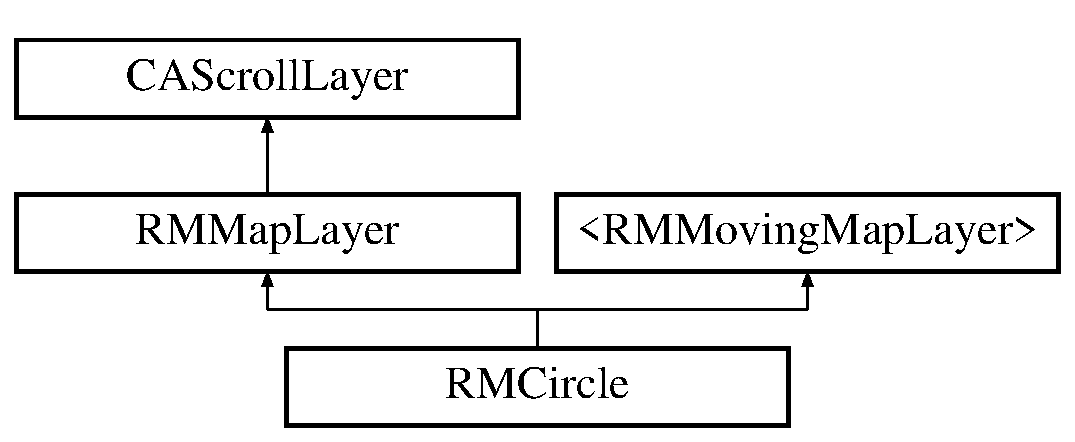
\includegraphics[height=3.000000cm]{interface_r_m_circle}
\end{center}
\end{figure}
\subsection*{Instance Methods}
\begin{DoxyCompactItemize}
\item 
(void) -\/ \hyperlink{interface_r_m_circle_acf8d3d162dee4f97d0c15932c8573bd1}{dealloc}{\ttfamily  \mbox{[}implementation\mbox{]}}
\item 
(id) -\/ \hyperlink{interface_r_m_circle_a0ec54a4b9dbdf85741f80d294e799d90}{init\-With\-Contents\-:radius\-In\-Meters\-:lat\-Long\-:}
\item 
(void) -\/ \hyperlink{interface_r_m_circle_ae75b2ad3001e194c07a13b53a2486871}{move\-By\-:}{\ttfamily  \mbox{[}implementation\mbox{]}}
\item 
(void) -\/ \hyperlink{interface_r_m_circle_a3499f453b9a9a25bc7c30419b35c7008}{move\-To\-Lat\-Long\-:}
\item 
(void) -\/ \hyperlink{interface_r_m_circle_a3fb94dae8c970736b643cf5293a55410}{set\-Fill\-Color\-:}{\ttfamily  \mbox{[}implementation\mbox{]}}
\item 
(void) -\/ \hyperlink{interface_r_m_circle_a8b50f3b1671b6de854aae4b49639120a}{set\-Line\-Color\-:}{\ttfamily  \mbox{[}implementation\mbox{]}}
\item 
(void) -\/ \hyperlink{interface_r_m_circle_a06cdb4f00d047443d030eafb63890c84}{set\-Line\-Width\-In\-Pixels\-:}{\ttfamily  \mbox{[}implementation\mbox{]}}
\item 
(void) -\/ \hyperlink{interface_r_m_circle_ac25b00f51cc70e84cad0c769df5e8a03}{set\-Projected\-Location\-:}{\ttfamily  \mbox{[}implementation\mbox{]}}
\item 
(void) -\/ \hyperlink{interface_r_m_circle_a7f2e47cbb3ad9b09db6cd705b4d8e070}{set\-Radius\-In\-Meters\-:}{\ttfamily  \mbox{[}implementation\mbox{]}}
\item 
(void) -\/ \hyperlink{interface_r_m_circle_a4dddcad3626f86cc77687e2465c212c8}{update\-Circle\-Path}{\ttfamily  \mbox{[}implementation\mbox{]}}
\item 
(void) -\/ \hyperlink{interface_r_m_circle_ad1cd9f88068ff39d6000f2bf9816cc2b}{zoom\-By\-Factor\-:near\-:}{\ttfamily  \mbox{[}implementation\mbox{]}}
\end{DoxyCompactItemize}
\subsection*{属性}
\begin{DoxyCompactItemize}
\item 
B\-O\-O\-L \hyperlink{interface_r_m_circle_ae3453eee968397a9ec223960f8f3df0f}{enable\-Dragging}
\item 
B\-O\-O\-L \hyperlink{interface_r_m_circle_ad3138252a9207ccb1639839ddb2c42b8}{enable\-Rotation}
\item 
U\-I\-Color $\ast$ \hyperlink{interface_r_m_circle_aa00ef131c513cfb8c540d092a733f3fe}{fill\-Color}
\item 
U\-I\-Color $\ast$ \hyperlink{interface_r_m_circle_a4d11b58b738e2bf11a6041d2388f63eb}{line\-Color}
\item 
C\-G\-Float \hyperlink{interface_r_m_circle_a3772331ca60c8812a35183c856983a17}{line\-Width\-In\-Pixels}
\item 
\hyperlink{struct_r_m_projected_point}{R\-M\-Projected\-Point} \hyperlink{interface_r_m_circle_a676b4e82ff075de3e4468a12f506006f}{projected\-Location}
\item 
C\-G\-Float \hyperlink{interface_r_m_circle_a9b20cc4c242976d1e4dec2439c31fc51}{radius\-In\-Meters}
\item 
C\-A\-Shape\-Layer $\ast$ \hyperlink{interface_r_m_circle_a7d1ee226bef3b061c4ca301957d91382}{shape\-Layer}
\end{DoxyCompactItemize}


\subsection{Method Documentation}
\hypertarget{interface_r_m_circle_acf8d3d162dee4f97d0c15932c8573bd1}{\index{R\-M\-Circle@{R\-M\-Circle}!dealloc@{dealloc}}
\index{dealloc@{dealloc}!RMCircle@{R\-M\-Circle}}
\subsubsection[{dealloc}]{\setlength{\rightskip}{0pt plus 5cm}-\/ (void) dealloc 
\begin{DoxyParamCaption}
{}
\end{DoxyParamCaption}
\hspace{0.3cm}{\ttfamily [implementation]}}}\label{interface_r_m_circle_acf8d3d162dee4f97d0c15932c8573bd1}
\hypertarget{interface_r_m_circle_a0ec54a4b9dbdf85741f80d294e799d90}{\index{R\-M\-Circle@{R\-M\-Circle}!init\-With\-Contents\-:radius\-In\-Meters\-:lat\-Long\-:@{init\-With\-Contents\-:radius\-In\-Meters\-:lat\-Long\-:}}
\index{init\-With\-Contents\-:radius\-In\-Meters\-:lat\-Long\-:@{init\-With\-Contents\-:radius\-In\-Meters\-:lat\-Long\-:}!RMCircle@{R\-M\-Circle}}
\subsubsection[{init\-With\-Contents\-:radius\-In\-Meters\-:lat\-Long\-:}]{\setlength{\rightskip}{0pt plus 5cm}-\/ (id) init\-With\-Contents\-: 
\begin{DoxyParamCaption}
\item[{({\bf R\-M\-Map\-Contents}$\ast$)}]{a\-Contents}
\item[{radiusInMeters:(C\-G\-Float)}]{new\-Radius\-In\-Meters}
\item[{latLong:({\bf R\-M\-Lat\-Long})}]{new\-Lat\-Long}
\end{DoxyParamCaption}
}}\label{interface_r_m_circle_a0ec54a4b9dbdf85741f80d294e799d90}
\hypertarget{interface_r_m_circle_ae75b2ad3001e194c07a13b53a2486871}{\index{R\-M\-Circle@{R\-M\-Circle}!move\-By\-:@{move\-By\-:}}
\index{move\-By\-:@{move\-By\-:}!RMCircle@{R\-M\-Circle}}
\subsubsection[{move\-By\-:}]{\setlength{\rightskip}{0pt plus 5cm}-\/ (void) move\-By\-: 
\begin{DoxyParamCaption}
\item[{(C\-G\-Size)}]{delta}
\end{DoxyParamCaption}
\hspace{0.3cm}{\ttfamily [implementation]}}}\label{interface_r_m_circle_ae75b2ad3001e194c07a13b53a2486871}


重载 \hyperlink{interface_r_m_map_layer_ac960944a80c596eb918531cf63c54c11}{R\-M\-Map\-Layer} .

\hypertarget{interface_r_m_circle_a3499f453b9a9a25bc7c30419b35c7008}{\index{R\-M\-Circle@{R\-M\-Circle}!move\-To\-Lat\-Long\-:@{move\-To\-Lat\-Long\-:}}
\index{move\-To\-Lat\-Long\-:@{move\-To\-Lat\-Long\-:}!RMCircle@{R\-M\-Circle}}
\subsubsection[{move\-To\-Lat\-Long\-:}]{\setlength{\rightskip}{0pt plus 5cm}-\/ (void) move\-To\-Lat\-Long\-: 
\begin{DoxyParamCaption}
\item[{({\bf R\-M\-Lat\-Long})}]{new\-Lat\-Long}
\end{DoxyParamCaption}
}}\label{interface_r_m_circle_a3499f453b9a9a25bc7c30419b35c7008}
\hypertarget{interface_r_m_circle_a3fb94dae8c970736b643cf5293a55410}{\index{R\-M\-Circle@{R\-M\-Circle}!set\-Fill\-Color\-:@{set\-Fill\-Color\-:}}
\index{set\-Fill\-Color\-:@{set\-Fill\-Color\-:}!RMCircle@{R\-M\-Circle}}
\subsubsection[{set\-Fill\-Color\-:}]{\setlength{\rightskip}{0pt plus 5cm}-\/ (void) set\-Fill\-Color\-: 
\begin{DoxyParamCaption}
\item[{(U\-I\-Color$\ast$)}]{new\-Fill\-Color}
\end{DoxyParamCaption}
\hspace{0.3cm}{\ttfamily [implementation]}}}\label{interface_r_m_circle_a3fb94dae8c970736b643cf5293a55410}
\hypertarget{interface_r_m_circle_a8b50f3b1671b6de854aae4b49639120a}{\index{R\-M\-Circle@{R\-M\-Circle}!set\-Line\-Color\-:@{set\-Line\-Color\-:}}
\index{set\-Line\-Color\-:@{set\-Line\-Color\-:}!RMCircle@{R\-M\-Circle}}
\subsubsection[{set\-Line\-Color\-:}]{\setlength{\rightskip}{0pt plus 5cm}-\/ (void) set\-Line\-Color\-: 
\begin{DoxyParamCaption}
\item[{(U\-I\-Color$\ast$)}]{new\-Line\-Color}
\end{DoxyParamCaption}
\hspace{0.3cm}{\ttfamily [implementation]}}}\label{interface_r_m_circle_a8b50f3b1671b6de854aae4b49639120a}
\hypertarget{interface_r_m_circle_a06cdb4f00d047443d030eafb63890c84}{\index{R\-M\-Circle@{R\-M\-Circle}!set\-Line\-Width\-In\-Pixels\-:@{set\-Line\-Width\-In\-Pixels\-:}}
\index{set\-Line\-Width\-In\-Pixels\-:@{set\-Line\-Width\-In\-Pixels\-:}!RMCircle@{R\-M\-Circle}}
\subsubsection[{set\-Line\-Width\-In\-Pixels\-:}]{\setlength{\rightskip}{0pt plus 5cm}-\/ (void) set\-Line\-Width\-In\-Pixels\-: 
\begin{DoxyParamCaption}
\item[{(C\-G\-Float)}]{new\-Line\-Width\-In\-Pixels}
\end{DoxyParamCaption}
\hspace{0.3cm}{\ttfamily [implementation]}}}\label{interface_r_m_circle_a06cdb4f00d047443d030eafb63890c84}
\hypertarget{interface_r_m_circle_ac25b00f51cc70e84cad0c769df5e8a03}{\index{R\-M\-Circle@{R\-M\-Circle}!set\-Projected\-Location\-:@{set\-Projected\-Location\-:}}
\index{set\-Projected\-Location\-:@{set\-Projected\-Location\-:}!RMCircle@{R\-M\-Circle}}
\subsubsection[{set\-Projected\-Location\-:}]{\setlength{\rightskip}{0pt plus 5cm}-\/ (void) set\-Projected\-Location\-: 
\begin{DoxyParamCaption}
\item[{({\bf R\-M\-Projected\-Point})}]{new\-Projected\-Location}
\end{DoxyParamCaption}
\hspace{0.3cm}{\ttfamily [implementation]}}}\label{interface_r_m_circle_ac25b00f51cc70e84cad0c769df5e8a03}


参考自 move\-To\-Lat\-Long\-:.

\hypertarget{interface_r_m_circle_a7f2e47cbb3ad9b09db6cd705b4d8e070}{\index{R\-M\-Circle@{R\-M\-Circle}!set\-Radius\-In\-Meters\-:@{set\-Radius\-In\-Meters\-:}}
\index{set\-Radius\-In\-Meters\-:@{set\-Radius\-In\-Meters\-:}!RMCircle@{R\-M\-Circle}}
\subsubsection[{set\-Radius\-In\-Meters\-:}]{\setlength{\rightskip}{0pt plus 5cm}-\/ (void) set\-Radius\-In\-Meters\-: 
\begin{DoxyParamCaption}
\item[{(C\-G\-Float)}]{new\-Radius\-In\-Meters}
\end{DoxyParamCaption}
\hspace{0.3cm}{\ttfamily [implementation]}}}\label{interface_r_m_circle_a7f2e47cbb3ad9b09db6cd705b4d8e070}
\hypertarget{interface_r_m_circle_a4dddcad3626f86cc77687e2465c212c8}{\index{R\-M\-Circle@{R\-M\-Circle}!update\-Circle\-Path@{update\-Circle\-Path}}
\index{update\-Circle\-Path@{update\-Circle\-Path}!RMCircle@{R\-M\-Circle}}
\subsubsection[{update\-Circle\-Path}]{\setlength{\rightskip}{0pt plus 5cm}-\/ (void) update\-Circle\-Path 
\begin{DoxyParamCaption}
{}
\end{DoxyParamCaption}
\hspace{0.3cm}{\ttfamily [implementation]}}}\label{interface_r_m_circle_a4dddcad3626f86cc77687e2465c212c8}


参考自 init\-With\-Contents\-:radius\-In\-Meters\-:lat\-Long\-:, set\-Fill\-Color\-:, set\-Line\-Color\-:, set\-Line\-Width\-In\-Pixels\-:, set\-Radius\-In\-Meters\-: , 以及 zoom\-By\-Factor\-:near\-:.

\hypertarget{interface_r_m_circle_ad1cd9f88068ff39d6000f2bf9816cc2b}{\index{R\-M\-Circle@{R\-M\-Circle}!zoom\-By\-Factor\-:near\-:@{zoom\-By\-Factor\-:near\-:}}
\index{zoom\-By\-Factor\-:near\-:@{zoom\-By\-Factor\-:near\-:}!RMCircle@{R\-M\-Circle}}
\subsubsection[{zoom\-By\-Factor\-:near\-:}]{\setlength{\rightskip}{0pt plus 5cm}-\/ (void) zoom\-By\-Factor\-: 
\begin{DoxyParamCaption}
\item[{(float)}]{zoom\-Factor}
\item[{near:(C\-G\-Point)}]{center}
\end{DoxyParamCaption}
\hspace{0.3cm}{\ttfamily [implementation]}}}\label{interface_r_m_circle_ad1cd9f88068ff39d6000f2bf9816cc2b}


重载 \hyperlink{interface_r_m_map_layer_ae0e1f8c364aaca4ac39766fe14bbba07}{R\-M\-Map\-Layer} .



\subsection{属性说明}
\hypertarget{interface_r_m_circle_ae3453eee968397a9ec223960f8f3df0f}{\index{R\-M\-Circle@{R\-M\-Circle}!enable\-Dragging@{enable\-Dragging}}
\index{enable\-Dragging@{enable\-Dragging}!RMCircle@{R\-M\-Circle}}
\subsubsection[{enable\-Dragging}]{\setlength{\rightskip}{0pt plus 5cm}-\/ (B\-O\-O\-L) enable\-Dragging\hspace{0.3cm}{\ttfamily [read]}, {\ttfamily [write]}, {\ttfamily [atomic]}, {\ttfamily [assign]}}}\label{interface_r_m_circle_ae3453eee968397a9ec223960f8f3df0f}


参考自 init\-With\-Contents\-:radius\-In\-Meters\-:lat\-Long\-: , 以及 move\-By\-:.

\hypertarget{interface_r_m_circle_ad3138252a9207ccb1639839ddb2c42b8}{\index{R\-M\-Circle@{R\-M\-Circle}!enable\-Rotation@{enable\-Rotation}}
\index{enable\-Rotation@{enable\-Rotation}!RMCircle@{R\-M\-Circle}}
\subsubsection[{enable\-Rotation}]{\setlength{\rightskip}{0pt plus 5cm}-\/ (B\-O\-O\-L) enable\-Rotation\hspace{0.3cm}{\ttfamily [read]}, {\ttfamily [write]}, {\ttfamily [atomic]}, {\ttfamily [assign]}}}\label{interface_r_m_circle_ad3138252a9207ccb1639839ddb2c42b8}


参考自 init\-With\-Contents\-:radius\-In\-Meters\-:lat\-Long\-:.

\hypertarget{interface_r_m_circle_aa00ef131c513cfb8c540d092a733f3fe}{\index{R\-M\-Circle@{R\-M\-Circle}!fill\-Color@{fill\-Color}}
\index{fill\-Color@{fill\-Color}!RMCircle@{R\-M\-Circle}}
\subsubsection[{fill\-Color}]{\setlength{\rightskip}{0pt plus 5cm}-\/ (U\-I\-Color $\ast$) fill\-Color\hspace{0.3cm}{\ttfamily [read]}, {\ttfamily [write]}, {\ttfamily [nonatomic]}, {\ttfamily [retain]}}}\label{interface_r_m_circle_aa00ef131c513cfb8c540d092a733f3fe}


参考自 dealloc, init\-With\-Contents\-:radius\-In\-Meters\-:lat\-Long\-:, set\-Fill\-Color\-: , 以及 update\-Circle\-Path.

\hypertarget{interface_r_m_circle_a4d11b58b738e2bf11a6041d2388f63eb}{\index{R\-M\-Circle@{R\-M\-Circle}!line\-Color@{line\-Color}}
\index{line\-Color@{line\-Color}!RMCircle@{R\-M\-Circle}}
\subsubsection[{line\-Color}]{\setlength{\rightskip}{0pt plus 5cm}-\/ (U\-I\-Color $\ast$) line\-Color\hspace{0.3cm}{\ttfamily [read]}, {\ttfamily [write]}, {\ttfamily [nonatomic]}, {\ttfamily [retain]}}}\label{interface_r_m_circle_a4d11b58b738e2bf11a6041d2388f63eb}


参考自 dealloc, init\-With\-Contents\-:radius\-In\-Meters\-:lat\-Long\-:, set\-Line\-Color\-: , 以及 update\-Circle\-Path.

\hypertarget{interface_r_m_circle_a3772331ca60c8812a35183c856983a17}{\index{R\-M\-Circle@{R\-M\-Circle}!line\-Width\-In\-Pixels@{line\-Width\-In\-Pixels}}
\index{line\-Width\-In\-Pixels@{line\-Width\-In\-Pixels}!RMCircle@{R\-M\-Circle}}
\subsubsection[{line\-Width\-In\-Pixels}]{\setlength{\rightskip}{0pt plus 5cm}-\/ (C\-G\-Float) line\-Width\-In\-Pixels\hspace{0.3cm}{\ttfamily [read]}, {\ttfamily [write]}, {\ttfamily [nonatomic]}, {\ttfamily [assign]}}}\label{interface_r_m_circle_a3772331ca60c8812a35183c856983a17}


参考自 init\-With\-Contents\-:radius\-In\-Meters\-:lat\-Long\-:, set\-Line\-Width\-In\-Pixels\-: , 以及 update\-Circle\-Path.

\hypertarget{interface_r_m_circle_a676b4e82ff075de3e4468a12f506006f}{\index{R\-M\-Circle@{R\-M\-Circle}!projected\-Location@{projected\-Location}}
\index{projected\-Location@{projected\-Location}!RMCircle@{R\-M\-Circle}}
\subsubsection[{projected\-Location}]{\setlength{\rightskip}{0pt plus 5cm}-\/ ({\bf R\-M\-Projected\-Point}) projected\-Location\hspace{0.3cm}{\ttfamily [read]}, {\ttfamily [write]}, {\ttfamily [nonatomic]}, {\ttfamily [assign]}}}\label{interface_r_m_circle_a676b4e82ff075de3e4468a12f506006f}


参考自 init\-With\-Contents\-:radius\-In\-Meters\-:lat\-Long\-: , 以及 set\-Projected\-Location\-:.

\hypertarget{interface_r_m_circle_a9b20cc4c242976d1e4dec2439c31fc51}{\index{R\-M\-Circle@{R\-M\-Circle}!radius\-In\-Meters@{radius\-In\-Meters}}
\index{radius\-In\-Meters@{radius\-In\-Meters}!RMCircle@{R\-M\-Circle}}
\subsubsection[{radius\-In\-Meters}]{\setlength{\rightskip}{0pt plus 5cm}-\/ (C\-G\-Float) radius\-In\-Meters\hspace{0.3cm}{\ttfamily [read]}, {\ttfamily [write]}, {\ttfamily [nonatomic]}, {\ttfamily [assign]}}}\label{interface_r_m_circle_a9b20cc4c242976d1e4dec2439c31fc51}


参考自 init\-With\-Contents\-:radius\-In\-Meters\-:lat\-Long\-:, set\-Radius\-In\-Meters\-: , 以及 update\-Circle\-Path.

\hypertarget{interface_r_m_circle_a7d1ee226bef3b061c4ca301957d91382}{\index{R\-M\-Circle@{R\-M\-Circle}!shape\-Layer@{shape\-Layer}}
\index{shape\-Layer@{shape\-Layer}!RMCircle@{R\-M\-Circle}}
\subsubsection[{shape\-Layer}]{\setlength{\rightskip}{0pt plus 5cm}-\/ (C\-A\-Shape\-Layer $\ast$) shape\-Layer\hspace{0.3cm}{\ttfamily [read]}, {\ttfamily [write]}, {\ttfamily [nonatomic]}, {\ttfamily [retain]}}}\label{interface_r_m_circle_a7d1ee226bef3b061c4ca301957d91382}


参考自 dealloc, init\-With\-Contents\-:radius\-In\-Meters\-:lat\-Long\-: , 以及 update\-Circle\-Path.



该类的文档由以下文件生成\-:\begin{DoxyCompactItemize}
\item 
Map/\hyperlink{_r_m_circle_8h}{R\-M\-Circle.\-h}\item 
Map/\hyperlink{_r_m_circle_8m}{R\-M\-Circle.\-m}\end{DoxyCompactItemize}

\hypertarget{interface_r_m_cloud_made_map_source}{\section{R\-M\-Cloud\-Made\-Map\-Source类 参考}
\label{interface_r_m_cloud_made_map_source}\index{R\-M\-Cloud\-Made\-Map\-Source@{R\-M\-Cloud\-Made\-Map\-Source}}
}


Subclass of \hyperlink{interface_r_m_abstract_mercator_web_source}{R\-M\-Abstract\-Mercator\-Web\-Source} for access to Cloud\-Made's commercial-\/grade tile servers.  




{\ttfamily \#import $<$R\-M\-Cloud\-Made\-Map\-Source.\-h$>$}

类 R\-M\-Cloud\-Made\-Map\-Source 继承关系图\-:\begin{figure}[H]
\begin{center}
\leavevmode
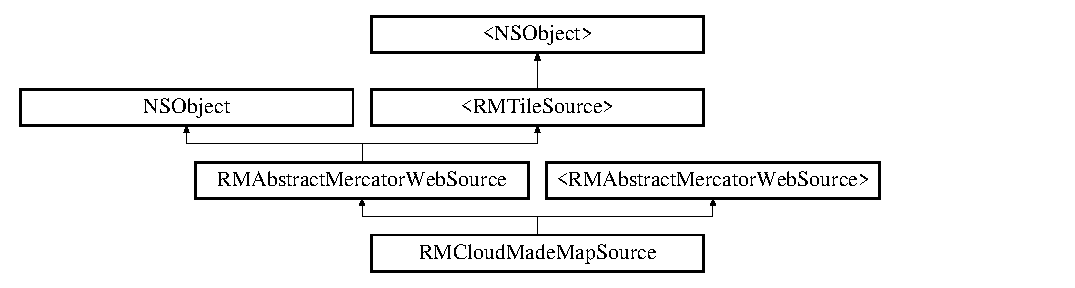
\includegraphics[height=3.425076cm]{interface_r_m_cloud_made_map_source}
\end{center}
\end{figure}
\subsection*{Instance Methods}
\begin{DoxyCompactItemize}
\item 
(id) -\/ \hyperlink{interface_r_m_cloud_made_map_source_ac1f36511f1261c96378989182fbdc724}{init}{\ttfamily  \mbox{[}implementation\mbox{]}}
\item 
(id) -\/ \hyperlink{interface_r_m_cloud_made_map_source_a604b3cd4b99894be4269193e9f860a83}{init\-With\-Access\-Key\-:style\-Number\-:}
\begin{DoxyCompactList}\small\item\em designated initializer \end{DoxyCompactList}\item 
(N\-S\-String $\ast$) -\/ \hyperlink{interface_r_m_cloud_made_map_source_a591d36a1e1d2d5d5024a568339542b5e}{long\-Attribution}{\ttfamily  \mbox{[}implementation\mbox{]}}
\item 
(N\-S\-String $\ast$) -\/ \hyperlink{interface_r_m_cloud_made_map_source_a0f04c8a09c3d1a9f25dcd4f45af2934b}{long\-Description}{\ttfamily  \mbox{[}implementation\mbox{]}}
\item 
(B\-O\-O\-L) -\/ \hyperlink{interface_r_m_cloud_made_map_source_a049018aa73338e739b40aa1c2aac811d}{read\-Token\-From\-File}{\ttfamily  \mbox{[}implementation\mbox{]}}
\item 
(void) -\/ \hyperlink{interface_r_m_cloud_made_map_source_a8e94aaa198d58bcf380dd9671bd063f8}{request\-Token}{\ttfamily  \mbox{[}implementation\mbox{]}}
\item 
(N\-S\-String $\ast$) -\/ \hyperlink{interface_r_m_cloud_made_map_source_a24b31ad20954e02ffde188c4a008d2e8}{short\-Attribution}{\ttfamily  \mbox{[}implementation\mbox{]}}
\item 
(N\-S\-String $\ast$) -\/ \hyperlink{interface_r_m_cloud_made_map_source_a5e956b126886325f16f34684d974262c}{short\-Name}{\ttfamily  \mbox{[}implementation\mbox{]}}
\item 
(N\-S\-String $\ast$) -\/ \hyperlink{interface_r_m_cloud_made_map_source_a25ff631fb042ace3eae48132f484a88e}{tile\-U\-R\-L\-:}{\ttfamily  \mbox{[}implementation\mbox{]}}
\item 
(N\-S\-String $\ast$) -\/ \hyperlink{interface_r_m_cloud_made_map_source_aae477f125ad88298f778b14b079a7bbb}{unique\-Tilecache\-Key}{\ttfamily  \mbox{[}implementation\mbox{]}}
\end{DoxyCompactItemize}
\subsection*{Class Methods}
\begin{DoxyCompactItemize}
\item 
(N\-S\-String $\ast$) + \hyperlink{interface_r_m_cloud_made_map_source_a472e70ed7bd9c453f9c536bccec94ef3}{path\-For\-Saved\-Access\-Token}{\ttfamily  \mbox{[}implementation\mbox{]}}
\end{DoxyCompactItemize}
\subsection*{Protected 属性}
\begin{DoxyCompactItemize}
\item 
N\-S\-String $\ast$ \hyperlink{interface_r_m_cloud_made_map_source_a4efefbc741e320d977cf04e9a96e02d0}{access\-Key}
\begin{DoxyCompactList}\small\item\em unique key identifying a particular developer/\-Cloud\-Made licensee. \end{DoxyCompactList}\item 
N\-S\-String $\ast$ \hyperlink{interface_r_m_cloud_made_map_source_ac3deb46e005ea4bdf67c0e32b4ab7406}{access\-Token}
\item 
N\-S\-U\-Integer \hyperlink{interface_r_m_cloud_made_map_source_a8fb92e3c3ae01146bc6a02bb437caec1}{cloudmade\-Style\-Number}
\begin{DoxyCompactList}\small\item\em see \href{http://maps.cloudmade.com/}{\tt http\-://maps.\-cloudmade.\-com/} to sample the various Cloud\-Made image styles \end{DoxyCompactList}\end{DoxyCompactItemize}


\subsection{详细描述}
Subclass of \hyperlink{interface_r_m_abstract_mercator_web_source}{R\-M\-Abstract\-Mercator\-Web\-Source} for access to Cloud\-Made's commercial-\/grade tile servers. 

Provides key-\/based access to tiles from Cloud\-Made's servers. This is Open Street Map data, but rendered much more nicely, in your choice of stylings. See \href{http://www.cloudmade.com/}{\tt http\-://www.\-cloudmade.\-com/} for licensing terms and fees. 

\subsection{Method Documentation}
\hypertarget{interface_r_m_cloud_made_map_source_ac1f36511f1261c96378989182fbdc724}{\index{R\-M\-Cloud\-Made\-Map\-Source@{R\-M\-Cloud\-Made\-Map\-Source}!init@{init}}
\index{init@{init}!RMCloudMadeMapSource@{R\-M\-Cloud\-Made\-Map\-Source}}
\subsubsection[{init}]{\setlength{\rightskip}{0pt plus 5cm}-\/ (id) init 
\begin{DoxyParamCaption}
{}
\end{DoxyParamCaption}
\hspace{0.3cm}{\ttfamily [implementation]}}}\label{interface_r_m_cloud_made_map_source_ac1f36511f1261c96378989182fbdc724}


重载 \hyperlink{interface_r_m_abstract_mercator_web_source_a88bc1ea00a789381d77ae50e0eaec732}{R\-M\-Abstract\-Mercator\-Web\-Source} .



参考自 init\-With\-Access\-Key\-:style\-Number\-:.

\hypertarget{interface_r_m_cloud_made_map_source_a604b3cd4b99894be4269193e9f860a83}{\index{R\-M\-Cloud\-Made\-Map\-Source@{R\-M\-Cloud\-Made\-Map\-Source}!init\-With\-Access\-Key\-:style\-Number\-:@{init\-With\-Access\-Key\-:style\-Number\-:}}
\index{init\-With\-Access\-Key\-:style\-Number\-:@{init\-With\-Access\-Key\-:style\-Number\-:}!RMCloudMadeMapSource@{R\-M\-Cloud\-Made\-Map\-Source}}
\subsubsection[{init\-With\-Access\-Key\-:style\-Number\-:}]{\setlength{\rightskip}{0pt plus 5cm}-\/ (id) init\-With\-Access\-Key\-: 
\begin{DoxyParamCaption}
\item[{(N\-S\-String $\ast$)}]{developer\-Access\-Key}
\item[{styleNumber:(N\-S\-U\-Integer)}]{style\-Number}
\end{DoxyParamCaption}
}}\label{interface_r_m_cloud_made_map_source_a604b3cd4b99894be4269193e9f860a83}


designated initializer 



参考自 init.

\hypertarget{interface_r_m_cloud_made_map_source_a591d36a1e1d2d5d5024a568339542b5e}{\index{R\-M\-Cloud\-Made\-Map\-Source@{R\-M\-Cloud\-Made\-Map\-Source}!long\-Attribution@{long\-Attribution}}
\index{long\-Attribution@{long\-Attribution}!RMCloudMadeMapSource@{R\-M\-Cloud\-Made\-Map\-Source}}
\subsubsection[{long\-Attribution}]{\setlength{\rightskip}{0pt plus 5cm}-\/ (N\-S\-String $\ast$) long\-Attribution 
\begin{DoxyParamCaption}
{}
\end{DoxyParamCaption}
\hspace{0.3cm}{\ttfamily [implementation]}}}\label{interface_r_m_cloud_made_map_source_a591d36a1e1d2d5d5024a568339542b5e}


重载 \hyperlink{interface_r_m_abstract_mercator_web_source_a77313c2d697428dd994a6e0cf07a256f}{R\-M\-Abstract\-Mercator\-Web\-Source} .

\hypertarget{interface_r_m_cloud_made_map_source_a0f04c8a09c3d1a9f25dcd4f45af2934b}{\index{R\-M\-Cloud\-Made\-Map\-Source@{R\-M\-Cloud\-Made\-Map\-Source}!long\-Description@{long\-Description}}
\index{long\-Description@{long\-Description}!RMCloudMadeMapSource@{R\-M\-Cloud\-Made\-Map\-Source}}
\subsubsection[{long\-Description}]{\setlength{\rightskip}{0pt plus 5cm}-\/ (N\-S\-String $\ast$) long\-Description 
\begin{DoxyParamCaption}
{}
\end{DoxyParamCaption}
\hspace{0.3cm}{\ttfamily [implementation]}}}\label{interface_r_m_cloud_made_map_source_a0f04c8a09c3d1a9f25dcd4f45af2934b}


重载 \hyperlink{interface_r_m_abstract_mercator_web_source_a9c1c86280c6fa05e4e82502822fcfd10}{R\-M\-Abstract\-Mercator\-Web\-Source} .

\hypertarget{interface_r_m_cloud_made_map_source_a472e70ed7bd9c453f9c536bccec94ef3}{\index{R\-M\-Cloud\-Made\-Map\-Source@{R\-M\-Cloud\-Made\-Map\-Source}!path\-For\-Saved\-Access\-Token@{path\-For\-Saved\-Access\-Token}}
\index{path\-For\-Saved\-Access\-Token@{path\-For\-Saved\-Access\-Token}!RMCloudMadeMapSource@{R\-M\-Cloud\-Made\-Map\-Source}}
\subsubsection[{path\-For\-Saved\-Access\-Token}]{\setlength{\rightskip}{0pt plus 5cm}+ (N\-S\-String $\ast$) path\-For\-Saved\-Access\-Token 
\begin{DoxyParamCaption}
{}
\end{DoxyParamCaption}
\hspace{0.3cm}{\ttfamily [implementation]}}}\label{interface_r_m_cloud_made_map_source_a472e70ed7bd9c453f9c536bccec94ef3}


参考自 read\-Token\-From\-File , 以及 request\-Token.

\hypertarget{interface_r_m_cloud_made_map_source_a049018aa73338e739b40aa1c2aac811d}{\index{R\-M\-Cloud\-Made\-Map\-Source@{R\-M\-Cloud\-Made\-Map\-Source}!read\-Token\-From\-File@{read\-Token\-From\-File}}
\index{read\-Token\-From\-File@{read\-Token\-From\-File}!RMCloudMadeMapSource@{R\-M\-Cloud\-Made\-Map\-Source}}
\subsubsection[{read\-Token\-From\-File}]{\setlength{\rightskip}{0pt plus 5cm}-\/ (B\-O\-O\-L) read\-Token\-From\-File 
\begin{DoxyParamCaption}
{}
\end{DoxyParamCaption}
\hspace{0.3cm}{\ttfamily [implementation]}}}\label{interface_r_m_cloud_made_map_source_a049018aa73338e739b40aa1c2aac811d}


参考自 request\-Token.

\hypertarget{interface_r_m_cloud_made_map_source_a8e94aaa198d58bcf380dd9671bd063f8}{\index{R\-M\-Cloud\-Made\-Map\-Source@{R\-M\-Cloud\-Made\-Map\-Source}!request\-Token@{request\-Token}}
\index{request\-Token@{request\-Token}!RMCloudMadeMapSource@{R\-M\-Cloud\-Made\-Map\-Source}}
\subsubsection[{request\-Token}]{\setlength{\rightskip}{0pt plus 5cm}-\/ (void) request\-Token 
\begin{DoxyParamCaption}
{}
\end{DoxyParamCaption}
\hspace{0.3cm}{\ttfamily [implementation]}}}\label{interface_r_m_cloud_made_map_source_a8e94aaa198d58bcf380dd9671bd063f8}


参考自 init\-With\-Access\-Key\-:style\-Number\-:.

\hypertarget{interface_r_m_cloud_made_map_source_a24b31ad20954e02ffde188c4a008d2e8}{\index{R\-M\-Cloud\-Made\-Map\-Source@{R\-M\-Cloud\-Made\-Map\-Source}!short\-Attribution@{short\-Attribution}}
\index{short\-Attribution@{short\-Attribution}!RMCloudMadeMapSource@{R\-M\-Cloud\-Made\-Map\-Source}}
\subsubsection[{short\-Attribution}]{\setlength{\rightskip}{0pt plus 5cm}-\/ (N\-S\-String $\ast$) short\-Attribution 
\begin{DoxyParamCaption}
{}
\end{DoxyParamCaption}
\hspace{0.3cm}{\ttfamily [implementation]}}}\label{interface_r_m_cloud_made_map_source_a24b31ad20954e02ffde188c4a008d2e8}


重载 \hyperlink{interface_r_m_abstract_mercator_web_source_a6be24cea169d058b5eefd7572bedc366}{R\-M\-Abstract\-Mercator\-Web\-Source} .

\hypertarget{interface_r_m_cloud_made_map_source_a5e956b126886325f16f34684d974262c}{\index{R\-M\-Cloud\-Made\-Map\-Source@{R\-M\-Cloud\-Made\-Map\-Source}!short\-Name@{short\-Name}}
\index{short\-Name@{short\-Name}!RMCloudMadeMapSource@{R\-M\-Cloud\-Made\-Map\-Source}}
\subsubsection[{short\-Name}]{\setlength{\rightskip}{0pt plus 5cm}-\/ (N\-S\-String $\ast$) short\-Name 
\begin{DoxyParamCaption}
{}
\end{DoxyParamCaption}
\hspace{0.3cm}{\ttfamily [implementation]}}}\label{interface_r_m_cloud_made_map_source_a5e956b126886325f16f34684d974262c}


重载 \hyperlink{interface_r_m_abstract_mercator_web_source_a3e6c6ef18250ce14317373db9df1fc85}{R\-M\-Abstract\-Mercator\-Web\-Source} .

\hypertarget{interface_r_m_cloud_made_map_source_a25ff631fb042ace3eae48132f484a88e}{\index{R\-M\-Cloud\-Made\-Map\-Source@{R\-M\-Cloud\-Made\-Map\-Source}!tile\-U\-R\-L\-:@{tile\-U\-R\-L\-:}}
\index{tile\-U\-R\-L\-:@{tile\-U\-R\-L\-:}!RMCloudMadeMapSource@{R\-M\-Cloud\-Made\-Map\-Source}}
\subsubsection[{tile\-U\-R\-L\-:}]{\setlength{\rightskip}{0pt plus 5cm}-\/ (N\-S\-String $\ast$) tile\-U\-R\-L\-: 
\begin{DoxyParamCaption}
\item[{({\bf R\-M\-Tile})}]{tile}
\end{DoxyParamCaption}
\hspace{0.3cm}{\ttfamily [implementation]}}}\label{interface_r_m_cloud_made_map_source_a25ff631fb042ace3eae48132f484a88e}


重载 \hyperlink{protocol_r_m_abstract_mercator_web_source-p_ae5c62f0fed7dcdfd78aa9582bdec9b4b}{$<$\-R\-M\-Abstract\-Mercator\-Web\-Source$>$} .

\hypertarget{interface_r_m_cloud_made_map_source_aae477f125ad88298f778b14b079a7bbb}{\index{R\-M\-Cloud\-Made\-Map\-Source@{R\-M\-Cloud\-Made\-Map\-Source}!unique\-Tilecache\-Key@{unique\-Tilecache\-Key}}
\index{unique\-Tilecache\-Key@{unique\-Tilecache\-Key}!RMCloudMadeMapSource@{R\-M\-Cloud\-Made\-Map\-Source}}
\subsubsection[{unique\-Tilecache\-Key}]{\setlength{\rightskip}{0pt plus 5cm}-\/ (N\-S\-String $\ast$) unique\-Tilecache\-Key 
\begin{DoxyParamCaption}
{}
\end{DoxyParamCaption}
\hspace{0.3cm}{\ttfamily [implementation]}}}\label{interface_r_m_cloud_made_map_source_aae477f125ad88298f778b14b079a7bbb}


重载 \hyperlink{interface_r_m_abstract_mercator_web_source_acf45b84d8f39ef7fcc2a92a2e320a9a2}{R\-M\-Abstract\-Mercator\-Web\-Source} .



\subsection{类成员变量说明}
\hypertarget{interface_r_m_cloud_made_map_source_a4efefbc741e320d977cf04e9a96e02d0}{\index{R\-M\-Cloud\-Made\-Map\-Source@{R\-M\-Cloud\-Made\-Map\-Source}!access\-Key@{access\-Key}}
\index{access\-Key@{access\-Key}!RMCloudMadeMapSource@{R\-M\-Cloud\-Made\-Map\-Source}}
\subsubsection[{access\-Key}]{\setlength{\rightskip}{0pt plus 5cm}-\/ (N\-S\-String$\ast$) access\-Key\hspace{0.3cm}{\ttfamily [protected]}}}\label{interface_r_m_cloud_made_map_source_a4efefbc741e320d977cf04e9a96e02d0}


unique key identifying a particular developer/\-Cloud\-Made licensee. 

See \href{http://developers.cloudmade.com/projects}{\tt http\-://developers.\-cloudmade.\-com/projects} to obtain a Cloud\-Made A\-P\-I key. 

参考自 init\-With\-Access\-Key\-:style\-Number\-:.

\hypertarget{interface_r_m_cloud_made_map_source_ac3deb46e005ea4bdf67c0e32b4ab7406}{\index{R\-M\-Cloud\-Made\-Map\-Source@{R\-M\-Cloud\-Made\-Map\-Source}!access\-Token@{access\-Token}}
\index{access\-Token@{access\-Token}!RMCloudMadeMapSource@{R\-M\-Cloud\-Made\-Map\-Source}}
\subsubsection[{access\-Token}]{\setlength{\rightskip}{0pt plus 5cm}-\/ (N\-S\-String$\ast$) access\-Token\hspace{0.3cm}{\ttfamily [protected]}}}\label{interface_r_m_cloud_made_map_source_ac3deb46e005ea4bdf67c0e32b4ab7406}


参考自 read\-Token\-From\-File, request\-Token , 以及 tile\-U\-R\-L\-:.

\hypertarget{interface_r_m_cloud_made_map_source_a8fb92e3c3ae01146bc6a02bb437caec1}{\index{R\-M\-Cloud\-Made\-Map\-Source@{R\-M\-Cloud\-Made\-Map\-Source}!cloudmade\-Style\-Number@{cloudmade\-Style\-Number}}
\index{cloudmade\-Style\-Number@{cloudmade\-Style\-Number}!RMCloudMadeMapSource@{R\-M\-Cloud\-Made\-Map\-Source}}
\subsubsection[{cloudmade\-Style\-Number}]{\setlength{\rightskip}{0pt plus 5cm}-\/ (N\-S\-U\-Integer) cloudmade\-Style\-Number\hspace{0.3cm}{\ttfamily [protected]}}}\label{interface_r_m_cloud_made_map_source_a8fb92e3c3ae01146bc6a02bb437caec1}


see \href{http://maps.cloudmade.com/}{\tt http\-://maps.\-cloudmade.\-com/} to sample the various Cloud\-Made image styles 



参考自 init\-With\-Access\-Key\-:style\-Number\-:.



该类的文档由以下文件生成\-:\begin{DoxyCompactItemize}
\item 
Map/\hyperlink{_r_m_cloud_made_map_source_8h}{R\-M\-Cloud\-Made\-Map\-Source.\-h}\item 
Map/\hyperlink{_r_m_cloud_made_map_source_8m}{R\-M\-Cloud\-Made\-Map\-Source.\-m}\end{DoxyCompactItemize}

\hypertarget{interface_r_m_cloud_map_source}{\section{R\-M\-Cloud\-Map\-Source类 参考}
\label{interface_r_m_cloud_map_source}\index{R\-M\-Cloud\-Map\-Source@{R\-M\-Cloud\-Map\-Source}}
}


Super\-Map云服务地图  




{\ttfamily \#import $<$R\-M\-Cloud\-Map\-Source.\-h$>$}

类 R\-M\-Cloud\-Map\-Source 继承关系图\-:\begin{figure}[H]
\begin{center}
\leavevmode
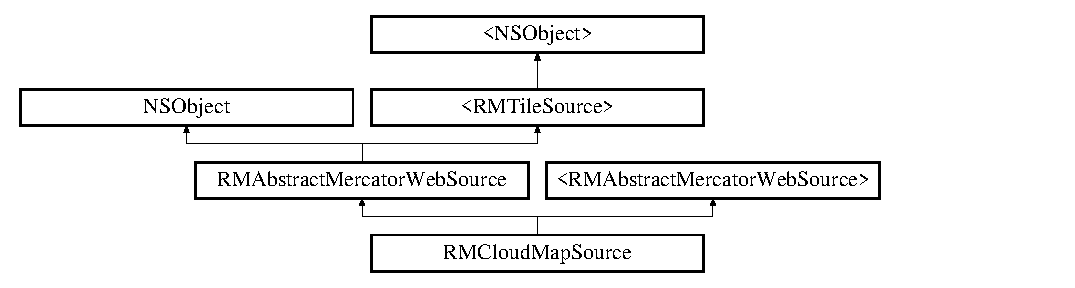
\includegraphics[height=3.425076cm]{interface_r_m_cloud_map_source}
\end{center}
\end{figure}
\subsection*{Instance Methods}
\begin{DoxyCompactItemize}
\item 
(id) -\/ \hyperlink{interface_r_m_cloud_map_source_af878223b3719bd71f274050374cd7cda}{init}{\ttfamily  \mbox{[}implementation\mbox{]}}
\item 
(N\-S\-String $\ast$) -\/ \hyperlink{interface_r_m_cloud_map_source_afc502c38dc65ff4ca970e7da5b39c5e1}{long\-Attribution}{\ttfamily  \mbox{[}implementation\mbox{]}}
\item 
(N\-S\-String $\ast$) -\/ \hyperlink{interface_r_m_cloud_map_source_a4c0753b3fee1264ceca0dd2fd46af299}{long\-Description}{\ttfamily  \mbox{[}implementation\mbox{]}}
\item 
(N\-S\-String $\ast$) -\/ \hyperlink{interface_r_m_cloud_map_source_ada3be85455de2b8dae2032035d870f3e}{short\-Attribution}{\ttfamily  \mbox{[}implementation\mbox{]}}
\item 
(N\-S\-String $\ast$) -\/ \hyperlink{interface_r_m_cloud_map_source_ad968ed767e547a7f97753e0ec34dec63}{short\-Name}{\ttfamily  \mbox{[}implementation\mbox{]}}
\item 
(N\-S\-String $\ast$) -\/ \hyperlink{interface_r_m_cloud_map_source_a13edb9f13639697b38732636d71688c1}{tile\-U\-R\-L\-:}{\ttfamily  \mbox{[}implementation\mbox{]}}
\item 
(N\-S\-String $\ast$) -\/ \hyperlink{interface_r_m_cloud_map_source_a7c4d7bb98a9fee5864622a1c5e342dd8}{unique\-Tilecache\-Key}{\ttfamily  \mbox{[}implementation\mbox{]}}
\end{DoxyCompactItemize}
\subsection*{额外继承的成员函数}


\subsection{详细描述}
Super\-Map云服务地图 

\subsection{Method Documentation}
\hypertarget{interface_r_m_cloud_map_source_af878223b3719bd71f274050374cd7cda}{\index{R\-M\-Cloud\-Map\-Source@{R\-M\-Cloud\-Map\-Source}!init@{init}}
\index{init@{init}!RMCloudMapSource@{R\-M\-Cloud\-Map\-Source}}
\subsubsection[{init}]{\setlength{\rightskip}{0pt plus 5cm}-\/ (id) init 
\begin{DoxyParamCaption}
{}
\end{DoxyParamCaption}
\hspace{0.3cm}{\ttfamily [implementation]}}}\label{interface_r_m_cloud_map_source_af878223b3719bd71f274050374cd7cda}


重载 \hyperlink{interface_r_m_abstract_mercator_web_source_a88bc1ea00a789381d77ae50e0eaec732}{R\-M\-Abstract\-Mercator\-Web\-Source} .

\hypertarget{interface_r_m_cloud_map_source_afc502c38dc65ff4ca970e7da5b39c5e1}{\index{R\-M\-Cloud\-Map\-Source@{R\-M\-Cloud\-Map\-Source}!long\-Attribution@{long\-Attribution}}
\index{long\-Attribution@{long\-Attribution}!RMCloudMapSource@{R\-M\-Cloud\-Map\-Source}}
\subsubsection[{long\-Attribution}]{\setlength{\rightskip}{0pt plus 5cm}-\/ (N\-S\-String $\ast$) long\-Attribution 
\begin{DoxyParamCaption}
{}
\end{DoxyParamCaption}
\hspace{0.3cm}{\ttfamily [implementation]}}}\label{interface_r_m_cloud_map_source_afc502c38dc65ff4ca970e7da5b39c5e1}


重载 \hyperlink{interface_r_m_abstract_mercator_web_source_a77313c2d697428dd994a6e0cf07a256f}{R\-M\-Abstract\-Mercator\-Web\-Source} .

\hypertarget{interface_r_m_cloud_map_source_a4c0753b3fee1264ceca0dd2fd46af299}{\index{R\-M\-Cloud\-Map\-Source@{R\-M\-Cloud\-Map\-Source}!long\-Description@{long\-Description}}
\index{long\-Description@{long\-Description}!RMCloudMapSource@{R\-M\-Cloud\-Map\-Source}}
\subsubsection[{long\-Description}]{\setlength{\rightskip}{0pt plus 5cm}-\/ (N\-S\-String $\ast$) long\-Description 
\begin{DoxyParamCaption}
{}
\end{DoxyParamCaption}
\hspace{0.3cm}{\ttfamily [implementation]}}}\label{interface_r_m_cloud_map_source_a4c0753b3fee1264ceca0dd2fd46af299}


重载 \hyperlink{interface_r_m_abstract_mercator_web_source_a9c1c86280c6fa05e4e82502822fcfd10}{R\-M\-Abstract\-Mercator\-Web\-Source} .

\hypertarget{interface_r_m_cloud_map_source_ada3be85455de2b8dae2032035d870f3e}{\index{R\-M\-Cloud\-Map\-Source@{R\-M\-Cloud\-Map\-Source}!short\-Attribution@{short\-Attribution}}
\index{short\-Attribution@{short\-Attribution}!RMCloudMapSource@{R\-M\-Cloud\-Map\-Source}}
\subsubsection[{short\-Attribution}]{\setlength{\rightskip}{0pt plus 5cm}-\/ (N\-S\-String $\ast$) short\-Attribution 
\begin{DoxyParamCaption}
{}
\end{DoxyParamCaption}
\hspace{0.3cm}{\ttfamily [implementation]}}}\label{interface_r_m_cloud_map_source_ada3be85455de2b8dae2032035d870f3e}


重载 \hyperlink{interface_r_m_abstract_mercator_web_source_a6be24cea169d058b5eefd7572bedc366}{R\-M\-Abstract\-Mercator\-Web\-Source} .

\hypertarget{interface_r_m_cloud_map_source_ad968ed767e547a7f97753e0ec34dec63}{\index{R\-M\-Cloud\-Map\-Source@{R\-M\-Cloud\-Map\-Source}!short\-Name@{short\-Name}}
\index{short\-Name@{short\-Name}!RMCloudMapSource@{R\-M\-Cloud\-Map\-Source}}
\subsubsection[{short\-Name}]{\setlength{\rightskip}{0pt plus 5cm}-\/ (N\-S\-String $\ast$) short\-Name 
\begin{DoxyParamCaption}
{}
\end{DoxyParamCaption}
\hspace{0.3cm}{\ttfamily [implementation]}}}\label{interface_r_m_cloud_map_source_ad968ed767e547a7f97753e0ec34dec63}


重载 \hyperlink{interface_r_m_abstract_mercator_web_source_a3e6c6ef18250ce14317373db9df1fc85}{R\-M\-Abstract\-Mercator\-Web\-Source} .

\hypertarget{interface_r_m_cloud_map_source_a13edb9f13639697b38732636d71688c1}{\index{R\-M\-Cloud\-Map\-Source@{R\-M\-Cloud\-Map\-Source}!tile\-U\-R\-L\-:@{tile\-U\-R\-L\-:}}
\index{tile\-U\-R\-L\-:@{tile\-U\-R\-L\-:}!RMCloudMapSource@{R\-M\-Cloud\-Map\-Source}}
\subsubsection[{tile\-U\-R\-L\-:}]{\setlength{\rightskip}{0pt plus 5cm}-\/ (N\-S\-String $\ast$) tile\-U\-R\-L\-: 
\begin{DoxyParamCaption}
\item[{({\bf R\-M\-Tile})}]{tile}
\end{DoxyParamCaption}
\hspace{0.3cm}{\ttfamily [implementation]}}}\label{interface_r_m_cloud_map_source_a13edb9f13639697b38732636d71688c1}


重载 \hyperlink{protocol_r_m_abstract_mercator_web_source-p_ae5c62f0fed7dcdfd78aa9582bdec9b4b}{$<$\-R\-M\-Abstract\-Mercator\-Web\-Source$>$} .

\hypertarget{interface_r_m_cloud_map_source_a7c4d7bb98a9fee5864622a1c5e342dd8}{\index{R\-M\-Cloud\-Map\-Source@{R\-M\-Cloud\-Map\-Source}!unique\-Tilecache\-Key@{unique\-Tilecache\-Key}}
\index{unique\-Tilecache\-Key@{unique\-Tilecache\-Key}!RMCloudMapSource@{R\-M\-Cloud\-Map\-Source}}
\subsubsection[{unique\-Tilecache\-Key}]{\setlength{\rightskip}{0pt plus 5cm}-\/ (N\-S\-String $\ast$) unique\-Tilecache\-Key 
\begin{DoxyParamCaption}
{}
\end{DoxyParamCaption}
\hspace{0.3cm}{\ttfamily [implementation]}}}\label{interface_r_m_cloud_map_source_a7c4d7bb98a9fee5864622a1c5e342dd8}


重载 \hyperlink{interface_r_m_abstract_mercator_web_source_acf45b84d8f39ef7fcc2a92a2e320a9a2}{R\-M\-Abstract\-Mercator\-Web\-Source} .



该类的文档由以下文件生成\-:\begin{DoxyCompactItemize}
\item 
Map/\hyperlink{_r_m_cloud_map_source_8h}{R\-M\-Cloud\-Map\-Source.\-h}\item 
Map/\hyperlink{_r_m_cloud_map_source_8m}{R\-M\-Cloud\-Map\-Source.\-m}\end{DoxyCompactItemize}

\hypertarget{interface_r_m_configuration}{\section{R\-M\-Configuration类 参考}
\label{interface_r_m_configuration}\index{R\-M\-Configuration@{R\-M\-Configuration}}
}


{\ttfamily \#import $<$R\-M\-Configuration.\-h$>$}

类 R\-M\-Configuration 继承关系图\-:\begin{figure}[H]
\begin{center}
\leavevmode
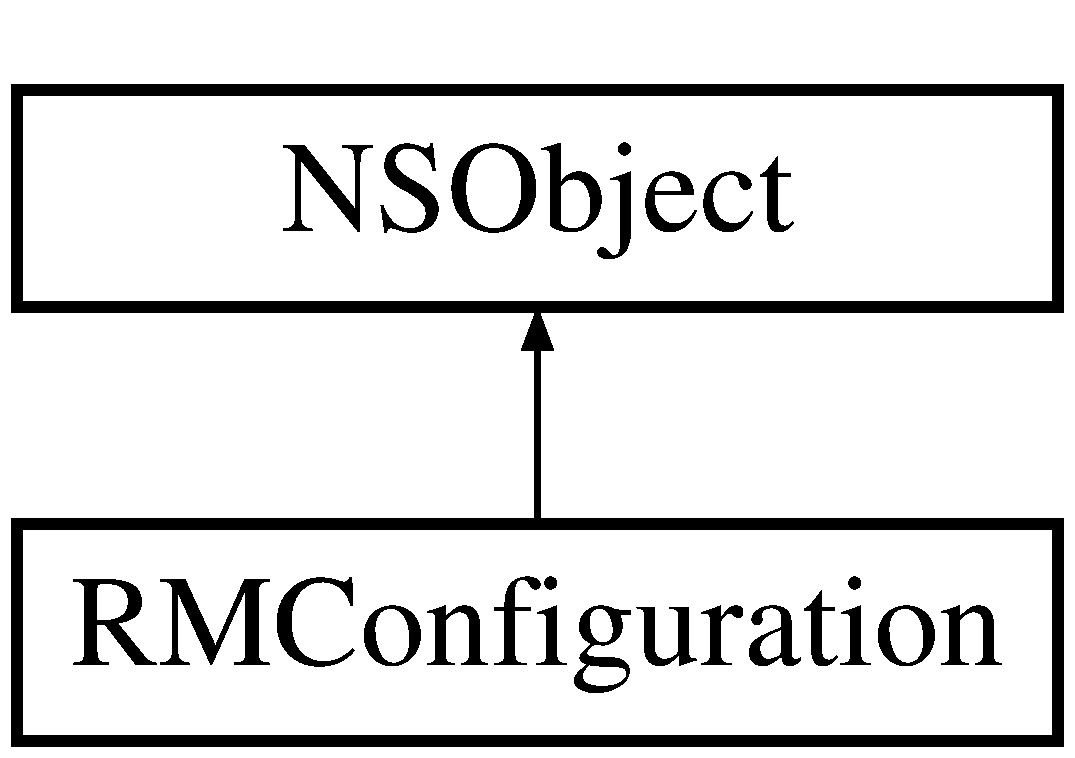
\includegraphics[height=2.000000cm]{interface_r_m_configuration}
\end{center}
\end{figure}
\subsection*{Instance Methods}
\begin{DoxyCompactItemize}
\item 
(N\-S\-Dictionary $\ast$) -\/ \hyperlink{interface_r_m_configuration_a7f29693a7f34f51433dda3129174b289}{cache\-Configuration}
\item 
(void) -\/ \hyperlink{interface_r_m_configuration_ad17b0c8a4b544a806b7e0b1d5ce4455d}{dealloc}
\item 
(\hyperlink{interface_r_m_configuration}{R\-M\-Configuration} $\ast$) -\/ \hyperlink{interface_r_m_configuration_a0eec9dc64f99eb0d43fc4a48542d91b0}{init\-With\-Path\-:}
\end{DoxyCompactItemize}
\subsection*{Class Methods}
\begin{DoxyCompactItemize}
\item 
(\hyperlink{interface_r_m_configuration}{R\-M\-Configuration} $\ast$) + \hyperlink{interface_r_m_configuration_ad6414afc2d914f013830974cdf9b9a43}{configuration}
\end{DoxyCompactItemize}
\subsection*{Protected 属性}
\begin{DoxyCompactItemize}
\item 
id \hyperlink{interface_r_m_configuration_a332a23cfb95e619572c9615033e04952}{prop\-List}
\end{DoxyCompactItemize}


\subsection{Method Documentation}
\hypertarget{interface_r_m_configuration_a7f29693a7f34f51433dda3129174b289}{\index{R\-M\-Configuration@{R\-M\-Configuration}!cache\-Configuration@{cache\-Configuration}}
\index{cache\-Configuration@{cache\-Configuration}!RMConfiguration@{R\-M\-Configuration}}
\subsubsection[{cache\-Configuration}]{\setlength{\rightskip}{0pt plus 5cm}-\/ (N\-S\-Dictionary $\ast$) cache\-Configuration 
\begin{DoxyParamCaption}
{}
\end{DoxyParamCaption}
}}\label{interface_r_m_configuration_a7f29693a7f34f51433dda3129174b289}
\begin{DoxyRefDesc}{Bug}
\item[\hyperlink{bug__bug000003}{Bug}]magic string literals \end{DoxyRefDesc}


参考自 R\-M\-Tile\-Cache\-::init\-With\-Tile\-Source\-:.

\hypertarget{interface_r_m_configuration_ad6414afc2d914f013830974cdf9b9a43}{\index{R\-M\-Configuration@{R\-M\-Configuration}!configuration@{configuration}}
\index{configuration@{configuration}!RMConfiguration@{R\-M\-Configuration}}
\subsubsection[{configuration}]{\setlength{\rightskip}{0pt plus 5cm}+ ({\bf R\-M\-Configuration} $\ast$) configuration 
\begin{DoxyParamCaption}
{}
\end{DoxyParamCaption}
}}\label{interface_r_m_configuration_ad6414afc2d914f013830974cdf9b9a43}
\begin{DoxyRefDesc}{Bug}
\item[\hyperlink{bug__bug000002}{Bug}]magic string literals \end{DoxyRefDesc}


参考自 R\-M\-Tile\-Cache\-::init\-With\-Tile\-Source\-:.

\hypertarget{interface_r_m_configuration_ad17b0c8a4b544a806b7e0b1d5ce4455d}{\index{R\-M\-Configuration@{R\-M\-Configuration}!dealloc@{dealloc}}
\index{dealloc@{dealloc}!RMConfiguration@{R\-M\-Configuration}}
\subsubsection[{dealloc}]{\setlength{\rightskip}{0pt plus 5cm}-\/ (void) dealloc 
\begin{DoxyParamCaption}
{}
\end{DoxyParamCaption}
}}\label{interface_r_m_configuration_ad17b0c8a4b544a806b7e0b1d5ce4455d}
\hypertarget{interface_r_m_configuration_a0eec9dc64f99eb0d43fc4a48542d91b0}{\index{R\-M\-Configuration@{R\-M\-Configuration}!init\-With\-Path\-:@{init\-With\-Path\-:}}
\index{init\-With\-Path\-:@{init\-With\-Path\-:}!RMConfiguration@{R\-M\-Configuration}}
\subsubsection[{init\-With\-Path\-:}]{\setlength{\rightskip}{0pt plus 5cm}-\/ ({\bf R\-M\-Configuration} $\ast$) init\-With\-Path\-: 
\begin{DoxyParamCaption}
\item[{(N\-S\-String$\ast$)}]{path}
\end{DoxyParamCaption}
}}\label{interface_r_m_configuration_a0eec9dc64f99eb0d43fc4a48542d91b0}


\subsection{类成员变量说明}
\hypertarget{interface_r_m_configuration_a332a23cfb95e619572c9615033e04952}{\index{R\-M\-Configuration@{R\-M\-Configuration}!prop\-List@{prop\-List}}
\index{prop\-List@{prop\-List}!RMConfiguration@{R\-M\-Configuration}}
\subsubsection[{prop\-List}]{\setlength{\rightskip}{0pt plus 5cm}-\/ (id) prop\-List\hspace{0.3cm}{\ttfamily [protected]}}}\label{interface_r_m_configuration_a332a23cfb95e619572c9615033e04952}


参考自 cache\-Configuration, dealloc , 以及 init\-With\-Path\-:.



该类的文档由以下文件生成\-:\begin{DoxyCompactItemize}
\item 
Map/\hyperlink{_r_m_configuration_8h}{R\-M\-Configuration.\-h}\item 
Map/\hyperlink{_r_m_configuration_8m}{R\-M\-Configuration.\-m}\end{DoxyCompactItemize}

\hypertarget{interface_r_m_core_animation_renderer}{\section{R\-M\-Core\-Animation\-Renderer类 参考}
\label{interface_r_m_core_animation_renderer}\index{R\-M\-Core\-Animation\-Renderer@{R\-M\-Core\-Animation\-Renderer}}
}


{\ttfamily \#import $<$R\-M\-Core\-Animation\-Renderer.\-h$>$}

类 R\-M\-Core\-Animation\-Renderer 继承关系图\-:\begin{figure}[H]
\begin{center}
\leavevmode
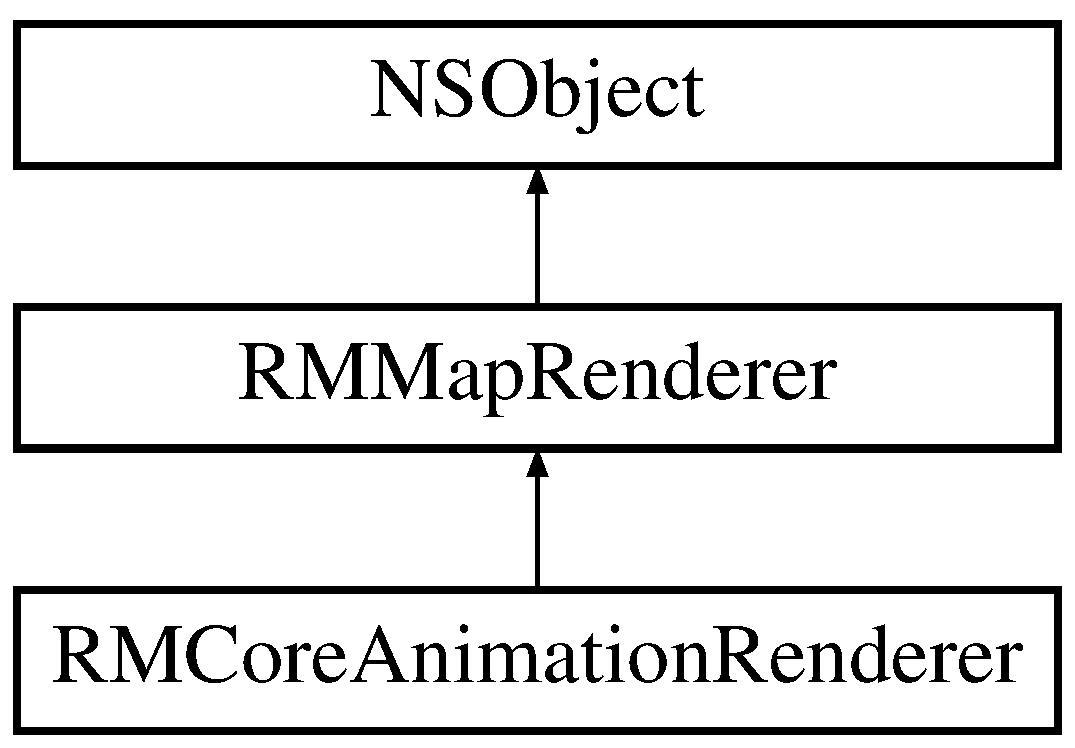
\includegraphics[height=3.000000cm]{interface_r_m_core_animation_renderer}
\end{center}
\end{figure}
\subsection*{Instance Methods}
\begin{DoxyCompactItemize}
\item 
(id$<$ C\-A\-Action $>$) -\/ \hyperlink{interface_r_m_core_animation_renderer_a479b29d8a064a627dacb4e8754288f84}{action\-For\-Layer\-:for\-Key\-:}{\ttfamily  \mbox{[}implementation\mbox{]}}
\item 
(void) -\/ \hyperlink{interface_r_m_core_animation_renderer_a042e89d2923653a122204ce1fa2efa70}{dealloc}{\ttfamily  \mbox{[}implementation\mbox{]}}
\item 
(id) -\/ \hyperlink{interface_r_m_core_animation_renderer_a0a684a7d8ba7065b4223b3079d8c3483}{init\-With\-Content\-:}{\ttfamily  \mbox{[}implementation\mbox{]}}
\item 
(C\-A\-Layer $\ast$) -\/ \hyperlink{interface_r_m_core_animation_renderer_ab37d6e7a835c2d88bc51bd4a21d5f5ca}{layer}{\ttfamily  \mbox{[}implementation\mbox{]}}
\item 
(void) -\/ \hyperlink{interface_r_m_core_animation_renderer_a0bf0f1d99f3d6b98583ae637139e245a}{map\-Image\-Loaded\-:}{\ttfamily  \mbox{[}implementation\mbox{]}}
\item 
(void) -\/ \hyperlink{interface_r_m_core_animation_renderer_ad46d40355e2c34bcf66663d802118035}{set\-Frame\-:}{\ttfamily  \mbox{[}implementation\mbox{]}}
\item 
(void) -\/ \hyperlink{interface_r_m_core_animation_renderer_adcf1987f0c72eb304d9c77f7f19cebc0}{tile\-Added\-:\-With\-Image\-:}{\ttfamily  \mbox{[}implementation\mbox{]}}
\item 
(void) -\/ \hyperlink{interface_r_m_core_animation_renderer_a14bbf63db3a350caaaa8c7e74eec8f3e}{tile\-Removed\-:}{\ttfamily  \mbox{[}implementation\mbox{]}}
\end{DoxyCompactItemize}
\subsection*{Protected 属性}
\begin{DoxyCompactItemize}
\item 
C\-A\-Layer $\ast$ \hyperlink{interface_r_m_core_animation_renderer_afdec0fc41c8cac5ee66303c3138f7dc9}{layer}
\item 
N\-S\-Mutable\-Array $\ast$ \hyperlink{interface_r_m_core_animation_renderer_ac99c17e8a4f0a759ef3482913ab05115}{tiles}
\end{DoxyCompactItemize}


\subsection{Method Documentation}
\hypertarget{interface_r_m_core_animation_renderer_a479b29d8a064a627dacb4e8754288f84}{\index{R\-M\-Core\-Animation\-Renderer@{R\-M\-Core\-Animation\-Renderer}!action\-For\-Layer\-:for\-Key\-:@{action\-For\-Layer\-:for\-Key\-:}}
\index{action\-For\-Layer\-:for\-Key\-:@{action\-For\-Layer\-:for\-Key\-:}!RMCoreAnimationRenderer@{R\-M\-Core\-Animation\-Renderer}}
\subsubsection[{action\-For\-Layer\-:for\-Key\-:}]{\setlength{\rightskip}{0pt plus 5cm}-\/ (id$<$ C\-A\-Action $>$) action\-For\-Layer\-: 
\begin{DoxyParamCaption}
\item[{(C\-A\-Layer $\ast$)}]{the\-Layer}
\item[{forKey:(N\-S\-String $\ast$)}]{key}
\end{DoxyParamCaption}
\hspace{0.3cm}{\ttfamily [implementation]}}}\label{interface_r_m_core_animation_renderer_a479b29d8a064a627dacb4e8754288f84}
\hypertarget{interface_r_m_core_animation_renderer_a042e89d2923653a122204ce1fa2efa70}{\index{R\-M\-Core\-Animation\-Renderer@{R\-M\-Core\-Animation\-Renderer}!dealloc@{dealloc}}
\index{dealloc@{dealloc}!RMCoreAnimationRenderer@{R\-M\-Core\-Animation\-Renderer}}
\subsubsection[{dealloc}]{\setlength{\rightskip}{0pt plus 5cm}-\/ (void) dealloc 
\begin{DoxyParamCaption}
{}
\end{DoxyParamCaption}
\hspace{0.3cm}{\ttfamily [implementation]}}}\label{interface_r_m_core_animation_renderer_a042e89d2923653a122204ce1fa2efa70}


重载 \hyperlink{interface_r_m_map_renderer_a171d7fd81412009ed1f92f27c5ec6f2a}{R\-M\-Map\-Renderer} .

\hypertarget{interface_r_m_core_animation_renderer_a0a684a7d8ba7065b4223b3079d8c3483}{\index{R\-M\-Core\-Animation\-Renderer@{R\-M\-Core\-Animation\-Renderer}!init\-With\-Content\-:@{init\-With\-Content\-:}}
\index{init\-With\-Content\-:@{init\-With\-Content\-:}!RMCoreAnimationRenderer@{R\-M\-Core\-Animation\-Renderer}}
\subsubsection[{init\-With\-Content\-:}]{\setlength{\rightskip}{0pt plus 5cm}-\/ (id) init\-With\-Content\-: 
\begin{DoxyParamCaption}
\item[{({\bf R\-M\-Map\-Contents} $\ast$)}]{\-\_\-contents}
\end{DoxyParamCaption}
\hspace{0.3cm}{\ttfamily [implementation]}}}\label{interface_r_m_core_animation_renderer_a0a684a7d8ba7065b4223b3079d8c3483}


重载 \hyperlink{interface_r_m_map_renderer_a439495e611ee8960c35d5272089f7b57}{R\-M\-Map\-Renderer} .

\hypertarget{interface_r_m_core_animation_renderer_ab37d6e7a835c2d88bc51bd4a21d5f5ca}{\index{R\-M\-Core\-Animation\-Renderer@{R\-M\-Core\-Animation\-Renderer}!layer@{layer}}
\index{layer@{layer}!RMCoreAnimationRenderer@{R\-M\-Core\-Animation\-Renderer}}
\subsubsection[{layer}]{\setlength{\rightskip}{0pt plus 5cm}-\/ (C\-A\-Layer $\ast$) layer 
\begin{DoxyParamCaption}
{}
\end{DoxyParamCaption}
\hspace{0.3cm}{\ttfamily [implementation]}}}\label{interface_r_m_core_animation_renderer_ab37d6e7a835c2d88bc51bd4a21d5f5ca}
\begin{DoxyRefDesc}{Bug}
\item[\hyperlink{bug__bug000023}{Bug}]no-\/op \end{DoxyRefDesc}


重载 \hyperlink{interface_r_m_map_renderer_a388de8a3bd1c56a07bc69f8967f34037}{R\-M\-Map\-Renderer} .



参考自 action\-For\-Layer\-:for\-Key\-:, dealloc, init\-With\-Content\-: , 以及 set\-Frame\-:.

\hypertarget{interface_r_m_core_animation_renderer_a0bf0f1d99f3d6b98583ae637139e245a}{\index{R\-M\-Core\-Animation\-Renderer@{R\-M\-Core\-Animation\-Renderer}!map\-Image\-Loaded\-:@{map\-Image\-Loaded\-:}}
\index{map\-Image\-Loaded\-:@{map\-Image\-Loaded\-:}!RMCoreAnimationRenderer@{R\-M\-Core\-Animation\-Renderer}}
\subsubsection[{map\-Image\-Loaded\-:}]{\setlength{\rightskip}{0pt plus 5cm}-\/ (void) map\-Image\-Loaded\-: 
\begin{DoxyParamCaption}
\item[{(N\-S\-Notification$\ast$)}]{notification}
\end{DoxyParamCaption}
\hspace{0.3cm}{\ttfamily [implementation]}}}\label{interface_r_m_core_animation_renderer_a0bf0f1d99f3d6b98583ae637139e245a}
\begin{DoxyRefDesc}{Bug}
\item[\hyperlink{bug__bug000004}{Bug}]this is a no-\/op \end{DoxyRefDesc}


重载 \hyperlink{interface_r_m_map_renderer_aa509a04f8b9702d4a4ea3010ca681f05}{R\-M\-Map\-Renderer} .

\hypertarget{interface_r_m_core_animation_renderer_ad46d40355e2c34bcf66663d802118035}{\index{R\-M\-Core\-Animation\-Renderer@{R\-M\-Core\-Animation\-Renderer}!set\-Frame\-:@{set\-Frame\-:}}
\index{set\-Frame\-:@{set\-Frame\-:}!RMCoreAnimationRenderer@{R\-M\-Core\-Animation\-Renderer}}
\subsubsection[{set\-Frame\-:}]{\setlength{\rightskip}{0pt plus 5cm}-\/ (void) set\-Frame\-: 
\begin{DoxyParamCaption}
\item[{(C\-G\-Rect)}]{frame}
\end{DoxyParamCaption}
\hspace{0.3cm}{\ttfamily [implementation]}}}\label{interface_r_m_core_animation_renderer_ad46d40355e2c34bcf66663d802118035}
\begin{DoxyRefDesc}{Bug}
\item[\hyperlink{bug__bug000022}{Bug}]no-\/op \end{DoxyRefDesc}


重载 \hyperlink{interface_r_m_map_renderer_a9191dc45f6215897f0e601e085850d1d}{R\-M\-Map\-Renderer} .

\hypertarget{interface_r_m_core_animation_renderer_adcf1987f0c72eb304d9c77f7f19cebc0}{\index{R\-M\-Core\-Animation\-Renderer@{R\-M\-Core\-Animation\-Renderer}!tile\-Added\-:\-With\-Image\-:@{tile\-Added\-:\-With\-Image\-:}}
\index{tile\-Added\-:\-With\-Image\-:@{tile\-Added\-:\-With\-Image\-:}!RMCoreAnimationRenderer@{R\-M\-Core\-Animation\-Renderer}}
\subsubsection[{tile\-Added\-:\-With\-Image\-:}]{\setlength{\rightskip}{0pt plus 5cm}-\/ (void) tile\-Added\-: 
\begin{DoxyParamCaption}
\item[{({\bf R\-M\-Tile})}]{tile}
\item[{WithImage:({\bf R\-M\-Tile\-Image}$\ast$)}]{image}
\end{DoxyParamCaption}
\hspace{0.3cm}{\ttfamily [implementation]}}}\label{interface_r_m_core_animation_renderer_adcf1987f0c72eb304d9c77f7f19cebc0}
\hypertarget{interface_r_m_core_animation_renderer_a14bbf63db3a350caaaa8c7e74eec8f3e}{\index{R\-M\-Core\-Animation\-Renderer@{R\-M\-Core\-Animation\-Renderer}!tile\-Removed\-:@{tile\-Removed\-:}}
\index{tile\-Removed\-:@{tile\-Removed\-:}!RMCoreAnimationRenderer@{R\-M\-Core\-Animation\-Renderer}}
\subsubsection[{tile\-Removed\-:}]{\setlength{\rightskip}{0pt plus 5cm}-\/ (void) tile\-Removed\-: 
\begin{DoxyParamCaption}
\item[{({\bf R\-M\-Tile})}]{tile}
\end{DoxyParamCaption}
\hspace{0.3cm}{\ttfamily [implementation]}}}\label{interface_r_m_core_animation_renderer_a14bbf63db3a350caaaa8c7e74eec8f3e}


\subsection{类成员变量说明}
\hypertarget{interface_r_m_core_animation_renderer_afdec0fc41c8cac5ee66303c3138f7dc9}{\index{R\-M\-Core\-Animation\-Renderer@{R\-M\-Core\-Animation\-Renderer}!layer@{layer}}
\index{layer@{layer}!RMCoreAnimationRenderer@{R\-M\-Core\-Animation\-Renderer}}
\subsubsection[{layer}]{\setlength{\rightskip}{0pt plus 5cm}-\/ (C\-A\-Layer$\ast$) layer\hspace{0.3cm}{\ttfamily [protected]}}}\label{interface_r_m_core_animation_renderer_afdec0fc41c8cac5ee66303c3138f7dc9}


参考自 dealloc, init\-With\-Content\-: , 以及 tile\-Added\-:\-With\-Image\-:.

\hypertarget{interface_r_m_core_animation_renderer_ac99c17e8a4f0a759ef3482913ab05115}{\index{R\-M\-Core\-Animation\-Renderer@{R\-M\-Core\-Animation\-Renderer}!tiles@{tiles}}
\index{tiles@{tiles}!RMCoreAnimationRenderer@{R\-M\-Core\-Animation\-Renderer}}
\subsubsection[{tiles}]{\setlength{\rightskip}{0pt plus 5cm}-\/ (N\-S\-Mutable\-Array$\ast$) tiles\hspace{0.3cm}{\ttfamily [protected]}}}\label{interface_r_m_core_animation_renderer_ac99c17e8a4f0a759ef3482913ab05115}


参考自 dealloc, init\-With\-Content\-:, tile\-Added\-:\-With\-Image\-: , 以及 tile\-Removed\-:.



该类的文档由以下文件生成\-:\begin{DoxyCompactItemize}
\item 
Map/\hyperlink{_r_m_core_animation_renderer_8h}{R\-M\-Core\-Animation\-Renderer.\-h}\item 
Map/\hyperlink{_r_m_core_animation_renderer_8m}{R\-M\-Core\-Animation\-Renderer.\-m}\end{DoxyCompactItemize}

\hypertarget{interface_r_m_database_cache}{\section{R\-M\-Database\-Cache类 参考}
\label{interface_r_m_database_cache}\index{R\-M\-Database\-Cache@{R\-M\-Database\-Cache}}
}


{\ttfamily \#import $<$R\-M\-Database\-Cache.\-h$>$}

类 R\-M\-Database\-Cache 继承关系图\-:\begin{figure}[H]
\begin{center}
\leavevmode
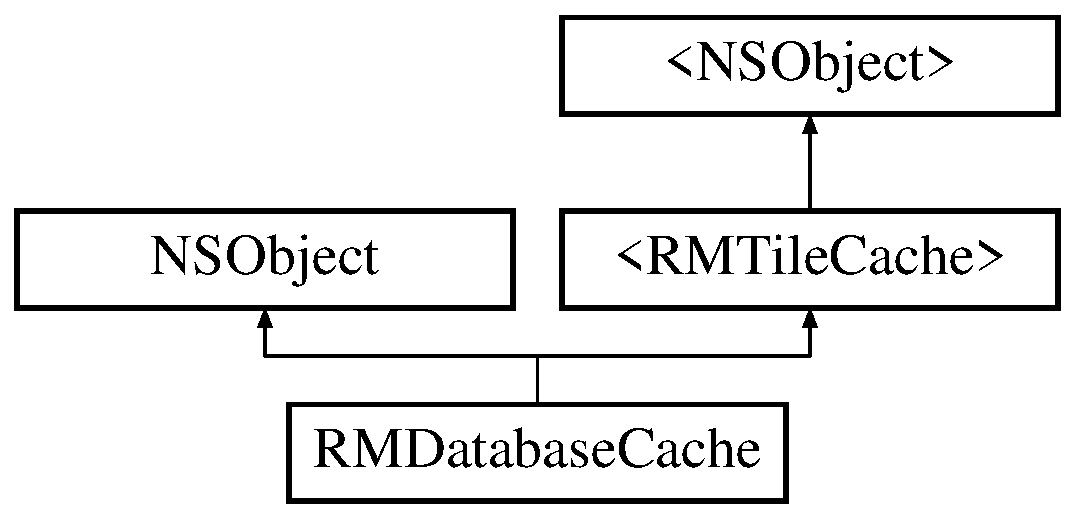
\includegraphics[height=3.000000cm]{interface_r_m_database_cache}
\end{center}
\end{figure}
\subsection*{Instance Methods}
\begin{DoxyCompactItemize}
\item 
(void) -\/ \hyperlink{interface_r_m_database_cache_ade3ba936e084cd27dd8baa6556df2409}{add\-Image\-Data\-:}{\ttfamily  \mbox{[}implementation\mbox{]}}
\item 
(void) -\/ \hyperlink{interface_r_m_database_cache_aa6e7191032fd7ee788d9566f93dcb124}{add\-Tile\-:\-With\-Image\-:}{\ttfamily  \mbox{[}implementation\mbox{]}}
\item 
(\hyperlink{interface_r_m_tile_image}{R\-M\-Tile\-Image} $\ast$) -\/ \hyperlink{interface_r_m_database_cache_a5b954b244864b84cc490815c841883fa}{cached\-Image\-:}{\ttfamily  \mbox{[}implementation\mbox{]}}
\begin{DoxyCompactList}\small\item\em Returns the cached image if it exists. nil otherwise. \end{DoxyCompactList}\item 
(void) -\/ \hyperlink{interface_r_m_database_cache_afbb97c4847de1495061d21d60e4e1066}{dealloc}{\ttfamily  \mbox{[}implementation\mbox{]}}
\item 
(void) -\/ \hyperlink{interface_r_m_database_cache_a22549fd820b0fb903d787b9235354199}{did\-Receive\-Memory\-Warning}{\ttfamily  \mbox{[}implementation\mbox{]}}
\item 
(id) -\/ \hyperlink{interface_r_m_database_cache_a19c0d0753815dc491d87f1a0a3c85ec6}{init\-With\-Database\-:}
\item 
(id) -\/ \hyperlink{interface_r_m_database_cache_a5991d40d229df8c26fc8f358ecafe569}{init\-With\-Tile\-Source\-:using\-Cache\-Dir\-:}
\item 
(void) -\/ \hyperlink{interface_r_m_database_cache_a03d0d4bee7287e82ca4db041a4434b1f}{purge\-Tiles\-From\-Before\-:}
\item 
(void) -\/ \hyperlink{interface_r_m_database_cache_a6b1d9c5a4c26b936ddd5bb837046760e}{remove\-All\-Cached\-Images}{\ttfamily  \mbox{[}implementation\mbox{]}}
\begin{DoxyCompactList}\small\item\em removes all tile images from the memory and disk subcaches \end{DoxyCompactList}\item 
(void) -\/ \hyperlink{interface_r_m_database_cache_a9815ce5f25d2dbc8f7f186e6d4ab9678}{set\-Capacity\-:}
\item 
(void) -\/ \hyperlink{interface_r_m_database_cache_a638f3d74205233c988fd727c163fc2bf}{set\-Minimal\-Purge\-:}
\item 
(void) -\/ \hyperlink{interface_r_m_database_cache_aefea28907d48132dbd79475ab385a497}{set\-Purge\-Strategy\-:}
\end{DoxyCompactItemize}
\subsection*{Class Methods}
\begin{DoxyCompactItemize}
\item 
(N\-S\-String $\ast$) + \hyperlink{interface_r_m_database_cache_a18cf19019d86081e29c6b57a903daefc}{db\-Path\-For\-Tile\-Source\-:using\-Cache\-Dir\-:}
\end{DoxyCompactItemize}
\subsection*{Protected 属性}
\begin{DoxyCompactItemize}
\item 
N\-S\-U\-Integer \hyperlink{interface_r_m_database_cache_afa03a8db5ae9ce39dcdfaaf4950198d0}{capacity}
\item 
\hyperlink{interface_r_m_tile_cache_d_a_o}{R\-M\-Tile\-Cache\-D\-A\-O} $\ast$ \hyperlink{interface_r_m_database_cache_a155c655a0a18d7fa99bae05faa17765c}{dao}
\item 
N\-S\-U\-Integer \hyperlink{interface_r_m_database_cache_af53a420e2e3f29269c0845a60efa3856}{minimal\-Purge}
\item 
\hyperlink{_r_m_tile_cache_8h_a39a51990ae35e2dbc42369aa64ef43f4}{R\-M\-Cache\-Purge\-Strategy} \hyperlink{interface_r_m_database_cache_a9504fb13d6065ee7a3cd5b37f500921d}{purge\-Strategy}
\end{DoxyCompactItemize}
\subsection*{属性}
\begin{DoxyCompactItemize}
\item 
N\-S\-String $\ast$ \hyperlink{interface_r_m_database_cache_a7c19186ec63b382cae1348a92b266ee7}{database\-Path}
\end{DoxyCompactItemize}


\subsection{Method Documentation}
\hypertarget{interface_r_m_database_cache_ade3ba936e084cd27dd8baa6556df2409}{\index{R\-M\-Database\-Cache@{R\-M\-Database\-Cache}!add\-Image\-Data\-:@{add\-Image\-Data\-:}}
\index{add\-Image\-Data\-:@{add\-Image\-Data\-:}!RMDatabaseCache@{R\-M\-Database\-Cache}}
\subsubsection[{add\-Image\-Data\-:}]{\setlength{\rightskip}{0pt plus 5cm}-\/ (void) add\-Image\-Data\-: 
\begin{DoxyParamCaption}
\item[{(N\-S\-Notification $\ast$)}]{notification}
\end{DoxyParamCaption}
\hspace{0.3cm}{\ttfamily [implementation]}}}\label{interface_r_m_database_cache_ade3ba936e084cd27dd8baa6556df2409}
\begin{DoxyRefDesc}{Bug}
\item[\hyperlink{bug__bug000006}{Bug}]magic string literals \end{DoxyRefDesc}
\hypertarget{interface_r_m_database_cache_aa6e7191032fd7ee788d9566f93dcb124}{\index{R\-M\-Database\-Cache@{R\-M\-Database\-Cache}!add\-Tile\-:\-With\-Image\-:@{add\-Tile\-:\-With\-Image\-:}}
\index{add\-Tile\-:\-With\-Image\-:@{add\-Tile\-:\-With\-Image\-:}!RMDatabaseCache@{R\-M\-Database\-Cache}}
\subsubsection[{add\-Tile\-:\-With\-Image\-:}]{\setlength{\rightskip}{0pt plus 5cm}-\/ (void) add\-Tile\-: 
\begin{DoxyParamCaption}
\item[{({\bf R\-M\-Tile})}]{tile}
\item[{WithImage:({\bf R\-M\-Tile\-Image}$\ast$)}]{image}
\end{DoxyParamCaption}
\hspace{0.3cm}{\ttfamily [implementation]}}}\label{interface_r_m_database_cache_aa6e7191032fd7ee788d9566f93dcb124}


重载 \hyperlink{protocol_r_m_tile_cache-p_a6a8e29b5f172b347d0ca556a643ee87c}{$<$\-R\-M\-Tile\-Cache$>$} .

\hypertarget{interface_r_m_database_cache_a5b954b244864b84cc490815c841883fa}{\index{R\-M\-Database\-Cache@{R\-M\-Database\-Cache}!cached\-Image\-:@{cached\-Image\-:}}
\index{cached\-Image\-:@{cached\-Image\-:}!RMDatabaseCache@{R\-M\-Database\-Cache}}
\subsubsection[{cached\-Image\-:}]{\setlength{\rightskip}{0pt plus 5cm}-\/ ({\bf R\-M\-Tile\-Image} $\ast$) cached\-Image\-: 
\begin{DoxyParamCaption}
\item[{({\bf R\-M\-Tile})}]{tile}
\end{DoxyParamCaption}
\hspace{0.3cm}{\ttfamily [implementation]}}}\label{interface_r_m_database_cache_a5b954b244864b84cc490815c841883fa}


Returns the cached image if it exists. nil otherwise. 



重载 \hyperlink{protocol_r_m_tile_cache-p_a4710bfa32e9aa99e8c8f6a335fcadbc2}{$<$\-R\-M\-Tile\-Cache$>$} .

\hypertarget{interface_r_m_database_cache_a18cf19019d86081e29c6b57a903daefc}{\index{R\-M\-Database\-Cache@{R\-M\-Database\-Cache}!db\-Path\-For\-Tile\-Source\-:using\-Cache\-Dir\-:@{db\-Path\-For\-Tile\-Source\-:using\-Cache\-Dir\-:}}
\index{db\-Path\-For\-Tile\-Source\-:using\-Cache\-Dir\-:@{db\-Path\-For\-Tile\-Source\-:using\-Cache\-Dir\-:}!RMDatabaseCache@{R\-M\-Database\-Cache}}
\subsubsection[{db\-Path\-For\-Tile\-Source\-:using\-Cache\-Dir\-:}]{\setlength{\rightskip}{0pt plus 5cm}+ (N\-S\-String $\ast$) db\-Path\-For\-Tile\-Source\-: 
\begin{DoxyParamCaption}
\item[{(id$<${\bf R\-M\-Tile\-Source}$>$)}]{source}
\item[{usingCacheDir:(B\-O\-O\-L)}]{use\-Cache\-Dir}
\end{DoxyParamCaption}
}}\label{interface_r_m_database_cache_a18cf19019d86081e29c6b57a903daefc}
\begin{DoxyRefDesc}{Bug}
\item[\hyperlink{bug__bug000005}{Bug}]magic string literals \end{DoxyRefDesc}


参考自 init\-With\-Tile\-Source\-:using\-Cache\-Dir\-:.

\hypertarget{interface_r_m_database_cache_afbb97c4847de1495061d21d60e4e1066}{\index{R\-M\-Database\-Cache@{R\-M\-Database\-Cache}!dealloc@{dealloc}}
\index{dealloc@{dealloc}!RMDatabaseCache@{R\-M\-Database\-Cache}}
\subsubsection[{dealloc}]{\setlength{\rightskip}{0pt plus 5cm}-\/ (void) dealloc 
\begin{DoxyParamCaption}
{}
\end{DoxyParamCaption}
\hspace{0.3cm}{\ttfamily [implementation]}}}\label{interface_r_m_database_cache_afbb97c4847de1495061d21d60e4e1066}
\hypertarget{interface_r_m_database_cache_a22549fd820b0fb903d787b9235354199}{\index{R\-M\-Database\-Cache@{R\-M\-Database\-Cache}!did\-Receive\-Memory\-Warning@{did\-Receive\-Memory\-Warning}}
\index{did\-Receive\-Memory\-Warning@{did\-Receive\-Memory\-Warning}!RMDatabaseCache@{R\-M\-Database\-Cache}}
\subsubsection[{did\-Receive\-Memory\-Warning}]{\setlength{\rightskip}{0pt plus 5cm}-\/ (void) did\-Receive\-Memory\-Warning 
\begin{DoxyParamCaption}
{}
\end{DoxyParamCaption}
\hspace{0.3cm}{\ttfamily [implementation]}}}\label{interface_r_m_database_cache_a22549fd820b0fb903d787b9235354199}


重载 \hyperlink{protocol_r_m_tile_cache-p_abd8c91f7aeefeeb8744537ed2f304449}{$<$\-R\-M\-Tile\-Cache$>$} .

\hypertarget{interface_r_m_database_cache_a19c0d0753815dc491d87f1a0a3c85ec6}{\index{R\-M\-Database\-Cache@{R\-M\-Database\-Cache}!init\-With\-Database\-:@{init\-With\-Database\-:}}
\index{init\-With\-Database\-:@{init\-With\-Database\-:}!RMDatabaseCache@{R\-M\-Database\-Cache}}
\subsubsection[{init\-With\-Database\-:}]{\setlength{\rightskip}{0pt plus 5cm}-\/ (id) init\-With\-Database\-: 
\begin{DoxyParamCaption}
\item[{(N\-S\-String$\ast$)}]{path}
\end{DoxyParamCaption}
}}\label{interface_r_m_database_cache_a19c0d0753815dc491d87f1a0a3c85ec6}


参考自 init\-With\-Tile\-Source\-:using\-Cache\-Dir\-:.

\hypertarget{interface_r_m_database_cache_a5991d40d229df8c26fc8f358ecafe569}{\index{R\-M\-Database\-Cache@{R\-M\-Database\-Cache}!init\-With\-Tile\-Source\-:using\-Cache\-Dir\-:@{init\-With\-Tile\-Source\-:using\-Cache\-Dir\-:}}
\index{init\-With\-Tile\-Source\-:using\-Cache\-Dir\-:@{init\-With\-Tile\-Source\-:using\-Cache\-Dir\-:}!RMDatabaseCache@{R\-M\-Database\-Cache}}
\subsubsection[{init\-With\-Tile\-Source\-:using\-Cache\-Dir\-:}]{\setlength{\rightskip}{0pt plus 5cm}-\/ (id) init\-With\-Tile\-Source\-: 
\begin{DoxyParamCaption}
\item[{(id$<${\bf R\-M\-Tile\-Source}$>$)}]{source}
\item[{usingCacheDir:(B\-O\-O\-L)}]{use\-Cache\-Dir}
\end{DoxyParamCaption}
}}\label{interface_r_m_database_cache_a5991d40d229df8c26fc8f358ecafe569}
\hypertarget{interface_r_m_database_cache_a03d0d4bee7287e82ca4db041a4434b1f}{\index{R\-M\-Database\-Cache@{R\-M\-Database\-Cache}!purge\-Tiles\-From\-Before\-:@{purge\-Tiles\-From\-Before\-:}}
\index{purge\-Tiles\-From\-Before\-:@{purge\-Tiles\-From\-Before\-:}!RMDatabaseCache@{R\-M\-Database\-Cache}}
\subsubsection[{purge\-Tiles\-From\-Before\-:}]{\setlength{\rightskip}{0pt plus 5cm}-\/ (void) purge\-Tiles\-From\-Before\-: 
\begin{DoxyParamCaption}
\item[{(N\-S\-Date$\ast$)}]{date}
\end{DoxyParamCaption}
}}\label{interface_r_m_database_cache_a03d0d4bee7287e82ca4db041a4434b1f}
\hypertarget{interface_r_m_database_cache_a6b1d9c5a4c26b936ddd5bb837046760e}{\index{R\-M\-Database\-Cache@{R\-M\-Database\-Cache}!remove\-All\-Cached\-Images@{remove\-All\-Cached\-Images}}
\index{remove\-All\-Cached\-Images@{remove\-All\-Cached\-Images}!RMDatabaseCache@{R\-M\-Database\-Cache}}
\subsubsection[{remove\-All\-Cached\-Images}]{\setlength{\rightskip}{0pt plus 5cm}-\/ (void) remove\-All\-Cached\-Images 
\begin{DoxyParamCaption}
{}
\end{DoxyParamCaption}
\hspace{0.3cm}{\ttfamily [implementation]}}}\label{interface_r_m_database_cache_a6b1d9c5a4c26b936ddd5bb837046760e}


removes all tile images from the memory and disk subcaches 



重载 \hyperlink{protocol_r_m_tile_cache-p_a57f54af62bb9c0e473ba2cd395864c4a}{$<$\-R\-M\-Tile\-Cache$>$} .

\hypertarget{interface_r_m_database_cache_a9815ce5f25d2dbc8f7f186e6d4ab9678}{\index{R\-M\-Database\-Cache@{R\-M\-Database\-Cache}!set\-Capacity\-:@{set\-Capacity\-:}}
\index{set\-Capacity\-:@{set\-Capacity\-:}!RMDatabaseCache@{R\-M\-Database\-Cache}}
\subsubsection[{set\-Capacity\-:}]{\setlength{\rightskip}{0pt plus 5cm}-\/ (void) set\-Capacity\-: 
\begin{DoxyParamCaption}
\item[{(N\-S\-U\-Integer)}]{the\-Capacity}
\end{DoxyParamCaption}
}}\label{interface_r_m_database_cache_a9815ce5f25d2dbc8f7f186e6d4ab9678}


参考自 R\-M\-Tile\-Cache\-::new\-Database\-Cache\-With\-Config\-:tile\-Source\-:.

\hypertarget{interface_r_m_database_cache_a638f3d74205233c988fd727c163fc2bf}{\index{R\-M\-Database\-Cache@{R\-M\-Database\-Cache}!set\-Minimal\-Purge\-:@{set\-Minimal\-Purge\-:}}
\index{set\-Minimal\-Purge\-:@{set\-Minimal\-Purge\-:}!RMDatabaseCache@{R\-M\-Database\-Cache}}
\subsubsection[{set\-Minimal\-Purge\-:}]{\setlength{\rightskip}{0pt plus 5cm}-\/ (void) set\-Minimal\-Purge\-: 
\begin{DoxyParamCaption}
\item[{(N\-S\-U\-Integer)}]{the\-Purge\-Minimum}
\end{DoxyParamCaption}
}}\label{interface_r_m_database_cache_a638f3d74205233c988fd727c163fc2bf}


参考自 R\-M\-Tile\-Cache\-::new\-Database\-Cache\-With\-Config\-:tile\-Source\-:.

\hypertarget{interface_r_m_database_cache_aefea28907d48132dbd79475ab385a497}{\index{R\-M\-Database\-Cache@{R\-M\-Database\-Cache}!set\-Purge\-Strategy\-:@{set\-Purge\-Strategy\-:}}
\index{set\-Purge\-Strategy\-:@{set\-Purge\-Strategy\-:}!RMDatabaseCache@{R\-M\-Database\-Cache}}
\subsubsection[{set\-Purge\-Strategy\-:}]{\setlength{\rightskip}{0pt plus 5cm}-\/ (void) set\-Purge\-Strategy\-: 
\begin{DoxyParamCaption}
\item[{({\bf R\-M\-Cache\-Purge\-Strategy})}]{the\-Strategy}
\end{DoxyParamCaption}
}}\label{interface_r_m_database_cache_aefea28907d48132dbd79475ab385a497}


参考自 R\-M\-Tile\-Cache\-::new\-Database\-Cache\-With\-Config\-:tile\-Source\-:.



\subsection{类成员变量说明}
\hypertarget{interface_r_m_database_cache_afa03a8db5ae9ce39dcdfaaf4950198d0}{\index{R\-M\-Database\-Cache@{R\-M\-Database\-Cache}!capacity@{capacity}}
\index{capacity@{capacity}!RMDatabaseCache@{R\-M\-Database\-Cache}}
\subsubsection[{capacity}]{\setlength{\rightskip}{0pt plus 5cm}-\/ (N\-S\-U\-Integer) capacity\hspace{0.3cm}{\ttfamily [protected]}}}\label{interface_r_m_database_cache_afa03a8db5ae9ce39dcdfaaf4950198d0}


参考自 add\-Image\-Data\-:, cached\-Image\-: , 以及 set\-Capacity\-:.

\hypertarget{interface_r_m_database_cache_a155c655a0a18d7fa99bae05faa17765c}{\index{R\-M\-Database\-Cache@{R\-M\-Database\-Cache}!dao@{dao}}
\index{dao@{dao}!RMDatabaseCache@{R\-M\-Database\-Cache}}
\subsubsection[{dao}]{\setlength{\rightskip}{0pt plus 5cm}-\/ ({\bf R\-M\-Tile\-Cache\-D\-A\-O}$\ast$) dao\hspace{0.3cm}{\ttfamily [protected]}}}\label{interface_r_m_database_cache_a155c655a0a18d7fa99bae05faa17765c}


参考自 add\-Image\-Data\-:, cached\-Image\-:, dealloc, did\-Receive\-Memory\-Warning, init\-With\-Database\-:, purge\-Tiles\-From\-Before\-: , 以及 remove\-All\-Cached\-Images.

\hypertarget{interface_r_m_database_cache_af53a420e2e3f29269c0845a60efa3856}{\index{R\-M\-Database\-Cache@{R\-M\-Database\-Cache}!minimal\-Purge@{minimal\-Purge}}
\index{minimal\-Purge@{minimal\-Purge}!RMDatabaseCache@{R\-M\-Database\-Cache}}
\subsubsection[{minimal\-Purge}]{\setlength{\rightskip}{0pt plus 5cm}-\/ (N\-S\-U\-Integer) minimal\-Purge\hspace{0.3cm}{\ttfamily [protected]}}}\label{interface_r_m_database_cache_af53a420e2e3f29269c0845a60efa3856}


参考自 set\-Minimal\-Purge\-:.

\hypertarget{interface_r_m_database_cache_a9504fb13d6065ee7a3cd5b37f500921d}{\index{R\-M\-Database\-Cache@{R\-M\-Database\-Cache}!purge\-Strategy@{purge\-Strategy}}
\index{purge\-Strategy@{purge\-Strategy}!RMDatabaseCache@{R\-M\-Database\-Cache}}
\subsubsection[{purge\-Strategy}]{\setlength{\rightskip}{0pt plus 5cm}-\/ ({\bf R\-M\-Cache\-Purge\-Strategy}) purge\-Strategy\hspace{0.3cm}{\ttfamily [protected]}}}\label{interface_r_m_database_cache_a9504fb13d6065ee7a3cd5b37f500921d}


参考自 cached\-Image\-: , 以及 set\-Purge\-Strategy\-:.



\subsection{属性说明}
\hypertarget{interface_r_m_database_cache_a7c19186ec63b382cae1348a92b266ee7}{\index{R\-M\-Database\-Cache@{R\-M\-Database\-Cache}!database\-Path@{database\-Path}}
\index{database\-Path@{database\-Path}!RMDatabaseCache@{R\-M\-Database\-Cache}}
\subsubsection[{database\-Path}]{\setlength{\rightskip}{0pt plus 5cm}-\/ (N\-S\-String $\ast$) database\-Path\hspace{0.3cm}{\ttfamily [read]}, {\ttfamily [write]}, {\ttfamily [atomic]}, {\ttfamily [retain]}}}\label{interface_r_m_database_cache_a7c19186ec63b382cae1348a92b266ee7}


参考自 dealloc.



该类的文档由以下文件生成\-:\begin{DoxyCompactItemize}
\item 
Map/\hyperlink{_r_m_database_cache_8h}{R\-M\-Database\-Cache.\-h}\item 
Map/\hyperlink{_r_m_database_cache_8m}{R\-M\-Database\-Cache.\-m}\end{DoxyCompactItemize}

\hypertarget{interface_r_m_d_b_map_source}{\section{R\-M\-D\-B\-Map\-Source类 参考}
\label{interface_r_m_d_b_map_source}\index{R\-M\-D\-B\-Map\-Source@{R\-M\-D\-B\-Map\-Source}}
}


{\ttfamily \#import $<$R\-M\-D\-B\-Map\-Source.\-h$>$}

类 R\-M\-D\-B\-Map\-Source 继承关系图\-:\begin{figure}[H]
\begin{center}
\leavevmode
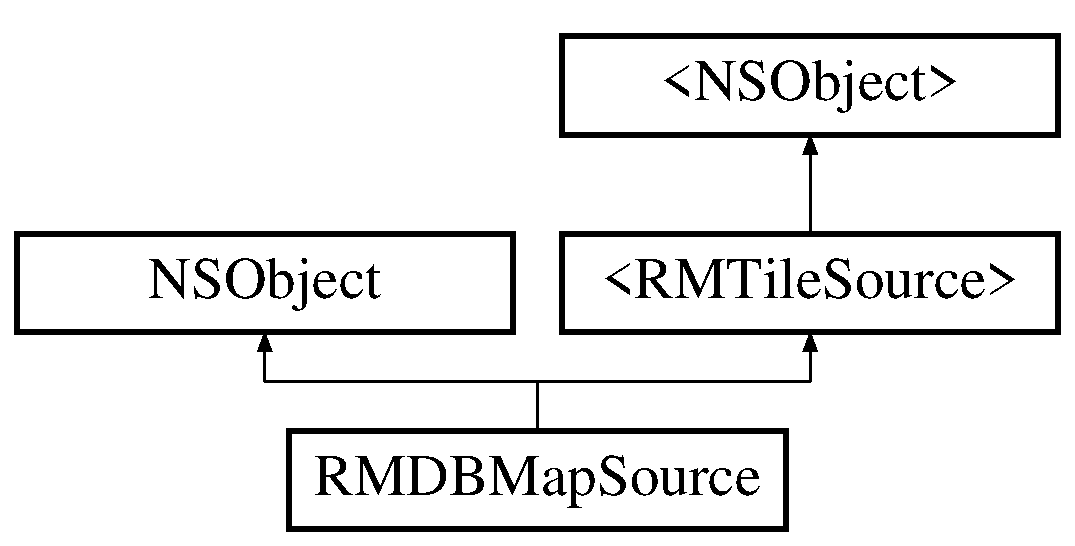
\includegraphics[height=3.000000cm]{interface_r_m_d_b_map_source}
\end{center}
\end{figure}
\subsection*{Instance Methods}
\begin{DoxyCompactItemize}
\item 
(C\-L\-Location\-Coordinate2\-D) -\/ \hyperlink{interface_r_m_d_b_map_source_a93c3633372135b528cc2465edb7b2ecd}{bottom\-Right\-Of\-Coverage}
\item 
(C\-L\-Location\-Coordinate2\-D) -\/ \hyperlink{interface_r_m_d_b_map_source_a56ec33f7059e7bfd4ded67ce6d6971a1}{center\-Of\-Coverage}
\item 
(void) -\/ \hyperlink{interface_r_m_d_b_map_source_a739f11524bff4d182ff4156f209ab029}{dealloc}{\ttfamily  \mbox{[}implementation\mbox{]}}
\item 
(void) -\/ \hyperlink{interface_r_m_d_b_map_source_a83c3f614b33aa51be649f9964d001e52}{did\-Receive\-Memory\-Warning}{\ttfamily  \mbox{[}implementation\mbox{]}}
\item 
(float) -\/ \hyperlink{interface_r_m_d_b_map_source_a42fa2b709c1cb908cb3e4b7594eb169d}{get\-Preference\-As\-Float\-:}{\ttfamily  \mbox{[}implementation\mbox{]}}
\item 
(int) -\/ \hyperlink{interface_r_m_d_b_map_source_abea886f3d6661dacc03af2b30190743d}{get\-Preference\-As\-Int\-:}{\ttfamily  \mbox{[}implementation\mbox{]}}
\item 
(N\-S\-String $\ast$) -\/ \hyperlink{interface_r_m_d_b_map_source_a38e204b65e0108a40c9649639eee77a5}{get\-Preference\-As\-String\-:}{\ttfamily  \mbox{[}implementation\mbox{]}}
\item 
(id) -\/ \hyperlink{interface_r_m_d_b_map_source_a19700da6a28ccf4d7de998a8eccb6bbe}{init\-With\-Path\-:}
\item 
(\hyperlink{struct_r_m_spherical_trapezium}{R\-M\-Spherical\-Trapezium}) -\/ \hyperlink{interface_r_m_d_b_map_source_a417dd7478c35cc11637d15dbcff47306}{latitude\-Longitude\-Bounding\-Box}{\ttfamily  \mbox{[}implementation\mbox{]}}
\item 
(N\-S\-String $\ast$) -\/ \hyperlink{interface_r_m_d_b_map_source_a8b7afccf2f64bd7f76e6ea093f765304}{long\-Attribution}
\item 
(N\-S\-String $\ast$) -\/ \hyperlink{interface_r_m_d_b_map_source_ae84c5c1f8b2d261ac0e148b43bcd17af}{long\-Description}
\item 
(float) -\/ \hyperlink{interface_r_m_d_b_map_source_a433624a4955d93aa353cf47c971243e2}{max\-Zoom}
\item 
(id$<$ \hyperlink{protocol_r_m_mercator_to_tile_projection-p}{R\-M\-Mercator\-To\-Tile\-Projection} $>$) -\/ \hyperlink{interface_r_m_d_b_map_source_ab8dfcb15d311db4fdc18e19173f31498}{mercator\-To\-Tile\-Projection}{\ttfamily  \mbox{[}implementation\mbox{]}}
\item 
(float) -\/ \hyperlink{interface_r_m_d_b_map_source_a8859704fadf0331beff1cd972ce0cae2}{min\-Zoom}
\item 
(\hyperlink{interface_r_m_projection}{R\-M\-Projection} $\ast$) -\/ \hyperlink{interface_r_m_d_b_map_source_aa1d33d38c216b461ef99176340aa4f66}{projection}{\ttfamily  \mbox{[}implementation\mbox{]}}
\item 
(void) -\/ \hyperlink{interface_r_m_d_b_map_source_a07b71c53e4e77a0a5913a77b8b6aed50}{remove\-All\-Cached\-Images}{\ttfamily  \mbox{[}implementation\mbox{]}}
\begin{DoxyCompactList}\small\item\em clear all images from the in-\/memory and on-\/disk image caches \end{DoxyCompactList}\item 
(void) -\/ \hyperlink{interface_r_m_d_b_map_source_a8bd95b34c6d17e645d898909c26555ad}{set\-Max\-Zoom\-:}{\ttfamily  \mbox{[}implementation\mbox{]}}
\item 
(void) -\/ \hyperlink{interface_r_m_d_b_map_source_adb54ef89f88b7aa129425d8dd01d1385}{set\-Min\-Zoom\-:}{\ttfamily  \mbox{[}implementation\mbox{]}}
\item 
(N\-S\-String $\ast$) -\/ \hyperlink{interface_r_m_d_b_map_source_a5d75085589beaaa6e8f2958f8c377cee}{short\-Attribution}
\item 
(N\-S\-String $\ast$) -\/ \hyperlink{interface_r_m_d_b_map_source_ab03a73ee305bf795ffa0a67aa64b4045}{short\-Name}
\item 
(N\-S\-String $\ast$) -\/ \hyperlink{interface_r_m_d_b_map_source_aa0d4904556d8b307f231b56c9c1c118c}{tile\-File\-:}{\ttfamily  \mbox{[}implementation\mbox{]}}
\item 
(\hyperlink{interface_r_m_tile_image}{R\-M\-Tile\-Image} $\ast$) -\/ \hyperlink{interface_r_m_d_b_map_source_a4cc3a54e7e1500edfcee3c5718bf602d}{tile\-Image\-:}{\ttfamily  \mbox{[}implementation\mbox{]}}
\item 
(N\-S\-String $\ast$) -\/ \hyperlink{interface_r_m_d_b_map_source_a809d089522cbd82f816feb7684b36c50}{tile\-Path}{\ttfamily  \mbox{[}implementation\mbox{]}}
\item 
(int) -\/ \hyperlink{interface_r_m_d_b_map_source_a91adbde1feb5d85af5f83ba6d6c29e51}{tile\-Side\-Length}
\item 
(N\-S\-String $\ast$) -\/ \hyperlink{interface_r_m_d_b_map_source_ae7bd74552105cc01a806bf9c2e91e140}{tile\-U\-R\-L\-:}{\ttfamily  \mbox{[}implementation\mbox{]}}
\item 
(C\-L\-Location\-Coordinate2\-D) -\/ \hyperlink{interface_r_m_d_b_map_source_a997830d307f04c1fafa025f23d3401f6}{top\-Left\-Of\-Coverage}
\item 
(N\-S\-String $\ast$) -\/ \hyperlink{interface_r_m_d_b_map_source_a49c20adf6dafd4221bdc2ea1a93077e0}{unique\-Tilecache\-Key}{\ttfamily  \mbox{[}implementation\mbox{]}}
\end{DoxyCompactItemize}
\subsection*{Protected 属性}
\begin{DoxyCompactItemize}
\item 
C\-L\-Location\-Coordinate2\-D \hyperlink{interface_r_m_d_b_map_source_ab2a40bc56609cd9b73603c54e8f6e0c5}{bottom\-Right}
\item 
C\-L\-Location\-Coordinate2\-D \hyperlink{interface_r_m_d_b_map_source_a507ddd273bc2a994d9d4fe5e4482baf5}{center}
\item 
F\-M\-Database $\ast$ \hyperlink{interface_r_m_d_b_map_source_a7a3b8f8155ec28765c51bc3543e5d630}{db}
\item 
float \hyperlink{interface_r_m_d_b_map_source_ad86d4d2b0eed882420b870bcb842233e}{max\-Zoom}
\item 
float \hyperlink{interface_r_m_d_b_map_source_a7f12d75beb479fbc8b50f2a8cf64a14b}{min\-Zoom}
\item 
\hyperlink{interface_r_m_fractal_tile_projection}{R\-M\-Fractal\-Tile\-Projection} $\ast$ \hyperlink{interface_r_m_d_b_map_source_a98ff222a2a972bf6cf4c317f4d7fa5dc}{tile\-Projection}
\item 
int \hyperlink{interface_r_m_d_b_map_source_a106cd606447ff75d7b81886d2b5a336f}{tile\-Side\-Length}
\item 
C\-L\-Location\-Coordinate2\-D \hyperlink{interface_r_m_d_b_map_source_aa8593714f212eeda83056518c4154606}{top\-Left}
\end{DoxyCompactItemize}


\subsection{Method Documentation}
\hypertarget{interface_r_m_d_b_map_source_a93c3633372135b528cc2465edb7b2ecd}{\index{R\-M\-D\-B\-Map\-Source@{R\-M\-D\-B\-Map\-Source}!bottom\-Right\-Of\-Coverage@{bottom\-Right\-Of\-Coverage}}
\index{bottom\-Right\-Of\-Coverage@{bottom\-Right\-Of\-Coverage}!RMDBMapSource@{R\-M\-D\-B\-Map\-Source}}
\subsubsection[{bottom\-Right\-Of\-Coverage}]{\setlength{\rightskip}{0pt plus 5cm}-\/ (C\-L\-Location\-Coordinate2\-D) bottom\-Right\-Of\-Coverage 
\begin{DoxyParamCaption}
{}
\end{DoxyParamCaption}
}}\label{interface_r_m_d_b_map_source_a93c3633372135b528cc2465edb7b2ecd}
\hypertarget{interface_r_m_d_b_map_source_a56ec33f7059e7bfd4ded67ce6d6971a1}{\index{R\-M\-D\-B\-Map\-Source@{R\-M\-D\-B\-Map\-Source}!center\-Of\-Coverage@{center\-Of\-Coverage}}
\index{center\-Of\-Coverage@{center\-Of\-Coverage}!RMDBMapSource@{R\-M\-D\-B\-Map\-Source}}
\subsubsection[{center\-Of\-Coverage}]{\setlength{\rightskip}{0pt plus 5cm}-\/ (C\-L\-Location\-Coordinate2\-D) center\-Of\-Coverage 
\begin{DoxyParamCaption}
{}
\end{DoxyParamCaption}
}}\label{interface_r_m_d_b_map_source_a56ec33f7059e7bfd4ded67ce6d6971a1}
\hypertarget{interface_r_m_d_b_map_source_a739f11524bff4d182ff4156f209ab029}{\index{R\-M\-D\-B\-Map\-Source@{R\-M\-D\-B\-Map\-Source}!dealloc@{dealloc}}
\index{dealloc@{dealloc}!RMDBMapSource@{R\-M\-D\-B\-Map\-Source}}
\subsubsection[{dealloc}]{\setlength{\rightskip}{0pt plus 5cm}-\/ (void) dealloc 
\begin{DoxyParamCaption}
{}
\end{DoxyParamCaption}
\hspace{0.3cm}{\ttfamily [implementation]}}}\label{interface_r_m_d_b_map_source_a739f11524bff4d182ff4156f209ab029}
\hypertarget{interface_r_m_d_b_map_source_a83c3f614b33aa51be649f9964d001e52}{\index{R\-M\-D\-B\-Map\-Source@{R\-M\-D\-B\-Map\-Source}!did\-Receive\-Memory\-Warning@{did\-Receive\-Memory\-Warning}}
\index{did\-Receive\-Memory\-Warning@{did\-Receive\-Memory\-Warning}!RMDBMapSource@{R\-M\-D\-B\-Map\-Source}}
\subsubsection[{did\-Receive\-Memory\-Warning}]{\setlength{\rightskip}{0pt plus 5cm}-\/ (void) did\-Receive\-Memory\-Warning 
\begin{DoxyParamCaption}
{}
\end{DoxyParamCaption}
\hspace{0.3cm}{\ttfamily [implementation]}}}\label{interface_r_m_d_b_map_source_a83c3f614b33aa51be649f9964d001e52}


重载 \hyperlink{protocol_r_m_tile_source-p_a70eade96883de23124c3f86321685b52}{$<$\-R\-M\-Tile\-Source$>$} .

\hypertarget{interface_r_m_d_b_map_source_a42fa2b709c1cb908cb3e4b7594eb169d}{\index{R\-M\-D\-B\-Map\-Source@{R\-M\-D\-B\-Map\-Source}!get\-Preference\-As\-Float\-:@{get\-Preference\-As\-Float\-:}}
\index{get\-Preference\-As\-Float\-:@{get\-Preference\-As\-Float\-:}!RMDBMapSource@{R\-M\-D\-B\-Map\-Source}}
\subsubsection[{get\-Preference\-As\-Float\-:}]{\setlength{\rightskip}{0pt plus 5cm}-\/ (float) get\-Preference\-As\-Float\-: 
\begin{DoxyParamCaption}
\item[{(N\-S\-String$\ast$)}]{name}
\end{DoxyParamCaption}
\hspace{0.3cm}{\ttfamily [implementation]}}}\label{interface_r_m_d_b_map_source_a42fa2b709c1cb908cb3e4b7594eb169d}


Provided by category \hyperlink{category_r_m_d_b_map_source_07_private_methods_08_a9379c8d39133b667b59f56e0662077e3}{R\-M\-D\-B\-Map\-Source(\-Private\-Methods)}.



参考自 init\-With\-Path\-:.

\hypertarget{interface_r_m_d_b_map_source_abea886f3d6661dacc03af2b30190743d}{\index{R\-M\-D\-B\-Map\-Source@{R\-M\-D\-B\-Map\-Source}!get\-Preference\-As\-Int\-:@{get\-Preference\-As\-Int\-:}}
\index{get\-Preference\-As\-Int\-:@{get\-Preference\-As\-Int\-:}!RMDBMapSource@{R\-M\-D\-B\-Map\-Source}}
\subsubsection[{get\-Preference\-As\-Int\-:}]{\setlength{\rightskip}{0pt plus 5cm}-\/ (int) get\-Preference\-As\-Int\-: 
\begin{DoxyParamCaption}
\item[{(N\-S\-String$\ast$)}]{name}
\end{DoxyParamCaption}
\hspace{0.3cm}{\ttfamily [implementation]}}}\label{interface_r_m_d_b_map_source_abea886f3d6661dacc03af2b30190743d}


Provided by category \hyperlink{category_r_m_d_b_map_source_07_private_methods_08_a220e5933f6ee9908550e7977f4dac4fd}{R\-M\-D\-B\-Map\-Source(\-Private\-Methods)}.



参考自 init\-With\-Path\-:.

\hypertarget{interface_r_m_d_b_map_source_a38e204b65e0108a40c9649639eee77a5}{\index{R\-M\-D\-B\-Map\-Source@{R\-M\-D\-B\-Map\-Source}!get\-Preference\-As\-String\-:@{get\-Preference\-As\-String\-:}}
\index{get\-Preference\-As\-String\-:@{get\-Preference\-As\-String\-:}!RMDBMapSource@{R\-M\-D\-B\-Map\-Source}}
\subsubsection[{get\-Preference\-As\-String\-:}]{\setlength{\rightskip}{0pt plus 5cm}-\/ (N\-S\-String $\ast$) get\-Preference\-As\-String\-: 
\begin{DoxyParamCaption}
\item[{(N\-S\-String$\ast$)}]{name}
\end{DoxyParamCaption}
\hspace{0.3cm}{\ttfamily [implementation]}}}\label{interface_r_m_d_b_map_source_a38e204b65e0108a40c9649639eee77a5}


Provided by category \hyperlink{category_r_m_d_b_map_source_07_private_methods_08_a2e1a62c671050d7ce0cf66cdc0b680e1}{R\-M\-D\-B\-Map\-Source(\-Private\-Methods)}.



参考自 get\-Preference\-As\-Float\-:, get\-Preference\-As\-Int\-:, long\-Attribution, long\-Description, short\-Attribution , 以及 short\-Name.

\hypertarget{interface_r_m_d_b_map_source_a19700da6a28ccf4d7de998a8eccb6bbe}{\index{R\-M\-D\-B\-Map\-Source@{R\-M\-D\-B\-Map\-Source}!init\-With\-Path\-:@{init\-With\-Path\-:}}
\index{init\-With\-Path\-:@{init\-With\-Path\-:}!RMDBMapSource@{R\-M\-D\-B\-Map\-Source}}
\subsubsection[{init\-With\-Path\-:}]{\setlength{\rightskip}{0pt plus 5cm}-\/ (id) init\-With\-Path\-: 
\begin{DoxyParamCaption}
\item[{(N\-S\-String$\ast$)}]{path}
\end{DoxyParamCaption}
}}\label{interface_r_m_d_b_map_source_a19700da6a28ccf4d7de998a8eccb6bbe}
\hypertarget{interface_r_m_d_b_map_source_a417dd7478c35cc11637d15dbcff47306}{\index{R\-M\-D\-B\-Map\-Source@{R\-M\-D\-B\-Map\-Source}!latitude\-Longitude\-Bounding\-Box@{latitude\-Longitude\-Bounding\-Box}}
\index{latitude\-Longitude\-Bounding\-Box@{latitude\-Longitude\-Bounding\-Box}!RMDBMapSource@{R\-M\-D\-B\-Map\-Source}}
\subsubsection[{latitude\-Longitude\-Bounding\-Box}]{\setlength{\rightskip}{0pt plus 5cm}-\/ ({\bf R\-M\-Spherical\-Trapezium}) latitude\-Longitude\-Bounding\-Box 
\begin{DoxyParamCaption}
{}
\end{DoxyParamCaption}
\hspace{0.3cm}{\ttfamily [implementation]}}}\label{interface_r_m_d_b_map_source_a417dd7478c35cc11637d15dbcff47306}


重载 \hyperlink{protocol_r_m_tile_source-p_a740893daebd1fe8e0a463e64a28816dd}{$<$\-R\-M\-Tile\-Source$>$} .

\hypertarget{interface_r_m_d_b_map_source_a8b7afccf2f64bd7f76e6ea093f765304}{\index{R\-M\-D\-B\-Map\-Source@{R\-M\-D\-B\-Map\-Source}!long\-Attribution@{long\-Attribution}}
\index{long\-Attribution@{long\-Attribution}!RMDBMapSource@{R\-M\-D\-B\-Map\-Source}}
\subsubsection[{long\-Attribution}]{\setlength{\rightskip}{0pt plus 5cm}-\/ (N\-S\-String $\ast$) long\-Attribution 
\begin{DoxyParamCaption}
{}
\end{DoxyParamCaption}
}}\label{interface_r_m_d_b_map_source_a8b7afccf2f64bd7f76e6ea093f765304}


重载 \hyperlink{protocol_r_m_tile_source-p_adff372c4c777906e56b90a61895d2ff4}{$<$\-R\-M\-Tile\-Source$>$} .

\hypertarget{interface_r_m_d_b_map_source_ae84c5c1f8b2d261ac0e148b43bcd17af}{\index{R\-M\-D\-B\-Map\-Source@{R\-M\-D\-B\-Map\-Source}!long\-Description@{long\-Description}}
\index{long\-Description@{long\-Description}!RMDBMapSource@{R\-M\-D\-B\-Map\-Source}}
\subsubsection[{long\-Description}]{\setlength{\rightskip}{0pt plus 5cm}-\/ (N\-S\-String $\ast$) long\-Description 
\begin{DoxyParamCaption}
{}
\end{DoxyParamCaption}
}}\label{interface_r_m_d_b_map_source_ae84c5c1f8b2d261ac0e148b43bcd17af}


重载 \hyperlink{protocol_r_m_tile_source-p_a1f9b03c3dac588a98b050afe3a71dcfa}{$<$\-R\-M\-Tile\-Source$>$} .

\hypertarget{interface_r_m_d_b_map_source_a433624a4955d93aa353cf47c971243e2}{\index{R\-M\-D\-B\-Map\-Source@{R\-M\-D\-B\-Map\-Source}!max\-Zoom@{max\-Zoom}}
\index{max\-Zoom@{max\-Zoom}!RMDBMapSource@{R\-M\-D\-B\-Map\-Source}}
\subsubsection[{max\-Zoom}]{\setlength{\rightskip}{0pt plus 5cm}-\/ (float) max\-Zoom 
\begin{DoxyParamCaption}
{}
\end{DoxyParamCaption}
}}\label{interface_r_m_d_b_map_source_a433624a4955d93aa353cf47c971243e2}


重载 \hyperlink{protocol_r_m_tile_source-p_a7d1ecfedd45c8ac433f972f38e7ac9a4}{$<$\-R\-M\-Tile\-Source$>$} .



参考自 init\-With\-Path\-:.

\hypertarget{interface_r_m_d_b_map_source_ab8dfcb15d311db4fdc18e19173f31498}{\index{R\-M\-D\-B\-Map\-Source@{R\-M\-D\-B\-Map\-Source}!mercator\-To\-Tile\-Projection@{mercator\-To\-Tile\-Projection}}
\index{mercator\-To\-Tile\-Projection@{mercator\-To\-Tile\-Projection}!RMDBMapSource@{R\-M\-D\-B\-Map\-Source}}
\subsubsection[{mercator\-To\-Tile\-Projection}]{\setlength{\rightskip}{0pt plus 5cm}-\/ (id$<$ {\bf R\-M\-Mercator\-To\-Tile\-Projection} $>$) mercator\-To\-Tile\-Projection 
\begin{DoxyParamCaption}
{}
\end{DoxyParamCaption}
\hspace{0.3cm}{\ttfamily [implementation]}}}\label{interface_r_m_d_b_map_source_ab8dfcb15d311db4fdc18e19173f31498}


重载 \hyperlink{protocol_r_m_tile_source-p_a5086edf762a1756058c665c3a9b0d26f}{$<$\-R\-M\-Tile\-Source$>$} .

\hypertarget{interface_r_m_d_b_map_source_a8859704fadf0331beff1cd972ce0cae2}{\index{R\-M\-D\-B\-Map\-Source@{R\-M\-D\-B\-Map\-Source}!min\-Zoom@{min\-Zoom}}
\index{min\-Zoom@{min\-Zoom}!RMDBMapSource@{R\-M\-D\-B\-Map\-Source}}
\subsubsection[{min\-Zoom}]{\setlength{\rightskip}{0pt plus 5cm}-\/ (float) min\-Zoom 
\begin{DoxyParamCaption}
{}
\end{DoxyParamCaption}
}}\label{interface_r_m_d_b_map_source_a8859704fadf0331beff1cd972ce0cae2}


重载 \hyperlink{protocol_r_m_tile_source-p_a7cd043d2bc55eded244b4c5da41dd909}{$<$\-R\-M\-Tile\-Source$>$} .



参考自 init\-With\-Path\-:.

\hypertarget{interface_r_m_d_b_map_source_aa1d33d38c216b461ef99176340aa4f66}{\index{R\-M\-D\-B\-Map\-Source@{R\-M\-D\-B\-Map\-Source}!projection@{projection}}
\index{projection@{projection}!RMDBMapSource@{R\-M\-D\-B\-Map\-Source}}
\subsubsection[{projection}]{\setlength{\rightskip}{0pt plus 5cm}-\/ ({\bf R\-M\-Projection} $\ast$) projection 
\begin{DoxyParamCaption}
{}
\end{DoxyParamCaption}
\hspace{0.3cm}{\ttfamily [implementation]}}}\label{interface_r_m_d_b_map_source_aa1d33d38c216b461ef99176340aa4f66}


重载 \hyperlink{protocol_r_m_tile_source-p_a75c20205e72db39aa01943d8b6d8fc29}{$<$\-R\-M\-Tile\-Source$>$} .



参考自 init\-With\-Path\-:.

\hypertarget{interface_r_m_d_b_map_source_a07b71c53e4e77a0a5913a77b8b6aed50}{\index{R\-M\-D\-B\-Map\-Source@{R\-M\-D\-B\-Map\-Source}!remove\-All\-Cached\-Images@{remove\-All\-Cached\-Images}}
\index{remove\-All\-Cached\-Images@{remove\-All\-Cached\-Images}!RMDBMapSource@{R\-M\-D\-B\-Map\-Source}}
\subsubsection[{remove\-All\-Cached\-Images}]{\setlength{\rightskip}{0pt plus 5cm}-\/ (void) remove\-All\-Cached\-Images 
\begin{DoxyParamCaption}
{}
\end{DoxyParamCaption}
\hspace{0.3cm}{\ttfamily [implementation]}}}\label{interface_r_m_d_b_map_source_a07b71c53e4e77a0a5913a77b8b6aed50}


clear all images from the in-\/memory and on-\/disk image caches 

\begin{DoxyRefDesc}{Bug}
\item[\hyperlink{bug__bug000052}{Bug}]This method belongs on \hyperlink{interface_r_m_cached_tile_source}{R\-M\-Cached\-Tile\-Source}, not on \hyperlink{protocol_r_m_tile_source-p}{R\-M\-Tile\-Source}, because an \hyperlink{protocol_r_m_tile_source-p}{R\-M\-Tile\-Source} doesn't have a cache. \end{DoxyRefDesc}


重载 \hyperlink{protocol_r_m_tile_source-p_aa5c4555fb2500e5826d5558985d4ee3c}{$<$\-R\-M\-Tile\-Source$>$} .

\hypertarget{interface_r_m_d_b_map_source_a8bd95b34c6d17e645d898909c26555ad}{\index{R\-M\-D\-B\-Map\-Source@{R\-M\-D\-B\-Map\-Source}!set\-Max\-Zoom\-:@{set\-Max\-Zoom\-:}}
\index{set\-Max\-Zoom\-:@{set\-Max\-Zoom\-:}!RMDBMapSource@{R\-M\-D\-B\-Map\-Source}}
\subsubsection[{set\-Max\-Zoom\-:}]{\setlength{\rightskip}{0pt plus 5cm}-\/ (void) set\-Max\-Zoom\-: 
\begin{DoxyParamCaption}
\item[{(N\-S\-U\-Integer)}]{a\-Max\-Zoom}
\end{DoxyParamCaption}
\hspace{0.3cm}{\ttfamily [implementation]}}}\label{interface_r_m_d_b_map_source_a8bd95b34c6d17e645d898909c26555ad}


重载 \hyperlink{protocol_r_m_tile_source-p_afd2310f2b3b95e91de2ef530ee5d5122}{$<$\-R\-M\-Tile\-Source$>$} .

\hypertarget{interface_r_m_d_b_map_source_adb54ef89f88b7aa129425d8dd01d1385}{\index{R\-M\-D\-B\-Map\-Source@{R\-M\-D\-B\-Map\-Source}!set\-Min\-Zoom\-:@{set\-Min\-Zoom\-:}}
\index{set\-Min\-Zoom\-:@{set\-Min\-Zoom\-:}!RMDBMapSource@{R\-M\-D\-B\-Map\-Source}}
\subsubsection[{set\-Min\-Zoom\-:}]{\setlength{\rightskip}{0pt plus 5cm}-\/ (void) set\-Min\-Zoom\-: 
\begin{DoxyParamCaption}
\item[{(N\-S\-U\-Integer)}]{a\-Min\-Zoom}
\end{DoxyParamCaption}
\hspace{0.3cm}{\ttfamily [implementation]}}}\label{interface_r_m_d_b_map_source_adb54ef89f88b7aa129425d8dd01d1385}


重载 \hyperlink{protocol_r_m_tile_source-p_ad8b2d3ab319784223970f215f6dd2f16}{$<$\-R\-M\-Tile\-Source$>$} .

\hypertarget{interface_r_m_d_b_map_source_a5d75085589beaaa6e8f2958f8c377cee}{\index{R\-M\-D\-B\-Map\-Source@{R\-M\-D\-B\-Map\-Source}!short\-Attribution@{short\-Attribution}}
\index{short\-Attribution@{short\-Attribution}!RMDBMapSource@{R\-M\-D\-B\-Map\-Source}}
\subsubsection[{short\-Attribution}]{\setlength{\rightskip}{0pt plus 5cm}-\/ (N\-S\-String $\ast$) short\-Attribution 
\begin{DoxyParamCaption}
{}
\end{DoxyParamCaption}
}}\label{interface_r_m_d_b_map_source_a5d75085589beaaa6e8f2958f8c377cee}


重载 \hyperlink{protocol_r_m_tile_source-p_afd67cfacb812cd3216ef1309297e264d}{$<$\-R\-M\-Tile\-Source$>$} .

\hypertarget{interface_r_m_d_b_map_source_ab03a73ee305bf795ffa0a67aa64b4045}{\index{R\-M\-D\-B\-Map\-Source@{R\-M\-D\-B\-Map\-Source}!short\-Name@{short\-Name}}
\index{short\-Name@{short\-Name}!RMDBMapSource@{R\-M\-D\-B\-Map\-Source}}
\subsubsection[{short\-Name}]{\setlength{\rightskip}{0pt plus 5cm}-\/ (N\-S\-String $\ast$) short\-Name 
\begin{DoxyParamCaption}
{}
\end{DoxyParamCaption}
}}\label{interface_r_m_d_b_map_source_ab03a73ee305bf795ffa0a67aa64b4045}


重载 \hyperlink{protocol_r_m_tile_source-p_ae0a98ebf46579f4c29d434322d25e64e}{$<$\-R\-M\-Tile\-Source$>$} .

\hypertarget{interface_r_m_d_b_map_source_aa0d4904556d8b307f231b56c9c1c118c}{\index{R\-M\-D\-B\-Map\-Source@{R\-M\-D\-B\-Map\-Source}!tile\-File\-:@{tile\-File\-:}}
\index{tile\-File\-:@{tile\-File\-:}!RMDBMapSource@{R\-M\-D\-B\-Map\-Source}}
\subsubsection[{tile\-File\-:}]{\setlength{\rightskip}{0pt plus 5cm}-\/ (N\-S\-String $\ast$) tile\-File\-: 
\begin{DoxyParamCaption}
\item[{({\bf R\-M\-Tile})}]{tile}
\end{DoxyParamCaption}
\hspace{0.3cm}{\ttfamily [implementation]}}}\label{interface_r_m_d_b_map_source_aa0d4904556d8b307f231b56c9c1c118c}


重载 \hyperlink{protocol_r_m_tile_source-p_adc40bd2f04352819fc05e32d4209a2ca}{$<$\-R\-M\-Tile\-Source$>$} .

\hypertarget{interface_r_m_d_b_map_source_a4cc3a54e7e1500edfcee3c5718bf602d}{\index{R\-M\-D\-B\-Map\-Source@{R\-M\-D\-B\-Map\-Source}!tile\-Image\-:@{tile\-Image\-:}}
\index{tile\-Image\-:@{tile\-Image\-:}!RMDBMapSource@{R\-M\-D\-B\-Map\-Source}}
\subsubsection[{tile\-Image\-:}]{\setlength{\rightskip}{0pt plus 5cm}-\/ ({\bf R\-M\-Tile\-Image} $\ast$) tile\-Image\-: 
\begin{DoxyParamCaption}
\item[{({\bf R\-M\-Tile})}]{tile}
\end{DoxyParamCaption}
\hspace{0.3cm}{\ttfamily [implementation]}}}\label{interface_r_m_d_b_map_source_a4cc3a54e7e1500edfcee3c5718bf602d}


重载 \hyperlink{protocol_r_m_tile_source-p_acf4ee01e3c1606d46a2ec8fe52b0d029}{$<$\-R\-M\-Tile\-Source$>$} .

\hypertarget{interface_r_m_d_b_map_source_a809d089522cbd82f816feb7684b36c50}{\index{R\-M\-D\-B\-Map\-Source@{R\-M\-D\-B\-Map\-Source}!tile\-Path@{tile\-Path}}
\index{tile\-Path@{tile\-Path}!RMDBMapSource@{R\-M\-D\-B\-Map\-Source}}
\subsubsection[{tile\-Path}]{\setlength{\rightskip}{0pt plus 5cm}-\/ (N\-S\-String $\ast$) tile\-Path 
\begin{DoxyParamCaption}
{}
\end{DoxyParamCaption}
\hspace{0.3cm}{\ttfamily [implementation]}}}\label{interface_r_m_d_b_map_source_a809d089522cbd82f816feb7684b36c50}


重载 \hyperlink{protocol_r_m_tile_source-p_ae9fc8d2cccf8a7ffce2a0f7837140b9b}{$<$\-R\-M\-Tile\-Source$>$} .

\hypertarget{interface_r_m_d_b_map_source_a91adbde1feb5d85af5f83ba6d6c29e51}{\index{R\-M\-D\-B\-Map\-Source@{R\-M\-D\-B\-Map\-Source}!tile\-Side\-Length@{tile\-Side\-Length}}
\index{tile\-Side\-Length@{tile\-Side\-Length}!RMDBMapSource@{R\-M\-D\-B\-Map\-Source}}
\subsubsection[{tile\-Side\-Length}]{\setlength{\rightskip}{0pt plus 5cm}-\/ (int) tile\-Side\-Length 
\begin{DoxyParamCaption}
{}
\end{DoxyParamCaption}
}}\label{interface_r_m_d_b_map_source_a91adbde1feb5d85af5f83ba6d6c29e51}


参考自 init\-With\-Path\-:.

\hypertarget{interface_r_m_d_b_map_source_ae7bd74552105cc01a806bf9c2e91e140}{\index{R\-M\-D\-B\-Map\-Source@{R\-M\-D\-B\-Map\-Source}!tile\-U\-R\-L\-:@{tile\-U\-R\-L\-:}}
\index{tile\-U\-R\-L\-:@{tile\-U\-R\-L\-:}!RMDBMapSource@{R\-M\-D\-B\-Map\-Source}}
\subsubsection[{tile\-U\-R\-L\-:}]{\setlength{\rightskip}{0pt plus 5cm}-\/ (N\-S\-String $\ast$) tile\-U\-R\-L\-: 
\begin{DoxyParamCaption}
\item[{({\bf R\-M\-Tile})}]{tile}
\end{DoxyParamCaption}
\hspace{0.3cm}{\ttfamily [implementation]}}}\label{interface_r_m_d_b_map_source_ae7bd74552105cc01a806bf9c2e91e140}


重载 \hyperlink{protocol_r_m_tile_source-p_af7ca2e2fb8e8cc4cb17433ffdc105230}{$<$\-R\-M\-Tile\-Source$>$} .

\hypertarget{interface_r_m_d_b_map_source_a997830d307f04c1fafa025f23d3401f6}{\index{R\-M\-D\-B\-Map\-Source@{R\-M\-D\-B\-Map\-Source}!top\-Left\-Of\-Coverage@{top\-Left\-Of\-Coverage}}
\index{top\-Left\-Of\-Coverage@{top\-Left\-Of\-Coverage}!RMDBMapSource@{R\-M\-D\-B\-Map\-Source}}
\subsubsection[{top\-Left\-Of\-Coverage}]{\setlength{\rightskip}{0pt plus 5cm}-\/ (C\-L\-Location\-Coordinate2\-D) top\-Left\-Of\-Coverage 
\begin{DoxyParamCaption}
{}
\end{DoxyParamCaption}
}}\label{interface_r_m_d_b_map_source_a997830d307f04c1fafa025f23d3401f6}
\hypertarget{interface_r_m_d_b_map_source_a49c20adf6dafd4221bdc2ea1a93077e0}{\index{R\-M\-D\-B\-Map\-Source@{R\-M\-D\-B\-Map\-Source}!unique\-Tilecache\-Key@{unique\-Tilecache\-Key}}
\index{unique\-Tilecache\-Key@{unique\-Tilecache\-Key}!RMDBMapSource@{R\-M\-D\-B\-Map\-Source}}
\subsubsection[{unique\-Tilecache\-Key}]{\setlength{\rightskip}{0pt plus 5cm}-\/ (N\-S\-String $\ast$) unique\-Tilecache\-Key 
\begin{DoxyParamCaption}
{}
\end{DoxyParamCaption}
\hspace{0.3cm}{\ttfamily [implementation]}}}\label{interface_r_m_d_b_map_source_a49c20adf6dafd4221bdc2ea1a93077e0}


重载 \hyperlink{protocol_r_m_tile_source-p_a1838a34e9341efe7c76252e131824261}{$<$\-R\-M\-Tile\-Source$>$} .



\subsection{类成员变量说明}
\hypertarget{interface_r_m_d_b_map_source_ab2a40bc56609cd9b73603c54e8f6e0c5}{\index{R\-M\-D\-B\-Map\-Source@{R\-M\-D\-B\-Map\-Source}!bottom\-Right@{bottom\-Right}}
\index{bottom\-Right@{bottom\-Right}!RMDBMapSource@{R\-M\-D\-B\-Map\-Source}}
\subsubsection[{bottom\-Right}]{\setlength{\rightskip}{0pt plus 5cm}-\/ (C\-L\-Location\-Coordinate2\-D) bottom\-Right\hspace{0.3cm}{\ttfamily [protected]}}}\label{interface_r_m_d_b_map_source_ab2a40bc56609cd9b73603c54e8f6e0c5}


参考自 bottom\-Right\-Of\-Coverage , 以及 init\-With\-Path\-:.

\hypertarget{interface_r_m_d_b_map_source_a507ddd273bc2a994d9d4fe5e4482baf5}{\index{R\-M\-D\-B\-Map\-Source@{R\-M\-D\-B\-Map\-Source}!center@{center}}
\index{center@{center}!RMDBMapSource@{R\-M\-D\-B\-Map\-Source}}
\subsubsection[{center}]{\setlength{\rightskip}{0pt plus 5cm}-\/ (C\-L\-Location\-Coordinate2\-D) center\hspace{0.3cm}{\ttfamily [protected]}}}\label{interface_r_m_d_b_map_source_a507ddd273bc2a994d9d4fe5e4482baf5}


参考自 center\-Of\-Coverage , 以及 init\-With\-Path\-:.

\hypertarget{interface_r_m_d_b_map_source_a7a3b8f8155ec28765c51bc3543e5d630}{\index{R\-M\-D\-B\-Map\-Source@{R\-M\-D\-B\-Map\-Source}!db@{db}}
\index{db@{db}!RMDBMapSource@{R\-M\-D\-B\-Map\-Source}}
\subsubsection[{db}]{\setlength{\rightskip}{0pt plus 5cm}-\/ (F\-M\-Database$\ast$) db\hspace{0.3cm}{\ttfamily [protected]}}}\label{interface_r_m_d_b_map_source_a7a3b8f8155ec28765c51bc3543e5d630}


参考自 dealloc, get\-Preference\-As\-String\-: , 以及 init\-With\-Path\-:.

\hypertarget{interface_r_m_d_b_map_source_ad86d4d2b0eed882420b870bcb842233e}{\index{R\-M\-D\-B\-Map\-Source@{R\-M\-D\-B\-Map\-Source}!max\-Zoom@{max\-Zoom}}
\index{max\-Zoom@{max\-Zoom}!RMDBMapSource@{R\-M\-D\-B\-Map\-Source}}
\subsubsection[{max\-Zoom}]{\setlength{\rightskip}{0pt plus 5cm}-\/ (float) max\-Zoom\hspace{0.3cm}{\ttfamily [protected]}}}\label{interface_r_m_d_b_map_source_ad86d4d2b0eed882420b870bcb842233e}
\hypertarget{interface_r_m_d_b_map_source_a7f12d75beb479fbc8b50f2a8cf64a14b}{\index{R\-M\-D\-B\-Map\-Source@{R\-M\-D\-B\-Map\-Source}!min\-Zoom@{min\-Zoom}}
\index{min\-Zoom@{min\-Zoom}!RMDBMapSource@{R\-M\-D\-B\-Map\-Source}}
\subsubsection[{min\-Zoom}]{\setlength{\rightskip}{0pt plus 5cm}-\/ (float) min\-Zoom\hspace{0.3cm}{\ttfamily [protected]}}}\label{interface_r_m_d_b_map_source_a7f12d75beb479fbc8b50f2a8cf64a14b}
\hypertarget{interface_r_m_d_b_map_source_a98ff222a2a972bf6cf4c317f4d7fa5dc}{\index{R\-M\-D\-B\-Map\-Source@{R\-M\-D\-B\-Map\-Source}!tile\-Projection@{tile\-Projection}}
\index{tile\-Projection@{tile\-Projection}!RMDBMapSource@{R\-M\-D\-B\-Map\-Source}}
\subsubsection[{tile\-Projection}]{\setlength{\rightskip}{0pt plus 5cm}-\/ ({\bf R\-M\-Fractal\-Tile\-Projection}$\ast$) tile\-Projection\hspace{0.3cm}{\ttfamily [protected]}}}\label{interface_r_m_d_b_map_source_a98ff222a2a972bf6cf4c317f4d7fa5dc}


参考自 dealloc, init\-With\-Path\-:, mercator\-To\-Tile\-Projection, set\-Max\-Zoom\-:, set\-Min\-Zoom\-: , 以及 tile\-Image\-:.

\hypertarget{interface_r_m_d_b_map_source_a106cd606447ff75d7b81886d2b5a336f}{\index{R\-M\-D\-B\-Map\-Source@{R\-M\-D\-B\-Map\-Source}!tile\-Side\-Length@{tile\-Side\-Length}}
\index{tile\-Side\-Length@{tile\-Side\-Length}!RMDBMapSource@{R\-M\-D\-B\-Map\-Source}}
\subsubsection[{tile\-Side\-Length}]{\setlength{\rightskip}{0pt plus 5cm}-\/ (int) tile\-Side\-Length\hspace{0.3cm}{\ttfamily [protected]}}}\label{interface_r_m_d_b_map_source_a106cd606447ff75d7b81886d2b5a336f}
\hypertarget{interface_r_m_d_b_map_source_aa8593714f212eeda83056518c4154606}{\index{R\-M\-D\-B\-Map\-Source@{R\-M\-D\-B\-Map\-Source}!top\-Left@{top\-Left}}
\index{top\-Left@{top\-Left}!RMDBMapSource@{R\-M\-D\-B\-Map\-Source}}
\subsubsection[{top\-Left}]{\setlength{\rightskip}{0pt plus 5cm}-\/ (C\-L\-Location\-Coordinate2\-D) top\-Left\hspace{0.3cm}{\ttfamily [protected]}}}\label{interface_r_m_d_b_map_source_aa8593714f212eeda83056518c4154606}


参考自 init\-With\-Path\-: , 以及 top\-Left\-Of\-Coverage.



该类的文档由以下文件生成\-:\begin{DoxyCompactItemize}
\item 
Map/\hyperlink{_r_m_d_b_map_source_8h}{R\-M\-D\-B\-Map\-Source.\-h}\item 
Map/\hyperlink{_r_m_d_b_map_source_8m}{R\-M\-D\-B\-Map\-Source.\-m}\end{DoxyCompactItemize}

\hypertarget{category_r_m_d_b_map_source_07_private_methods_08}{\section{R\-M\-D\-B\-Map\-Source(Private\-Methods)分类 参考}
\label{category_r_m_d_b_map_source_07_private_methods_08}\index{R\-M\-D\-B\-Map\-Source(\-Private\-Methods)@{R\-M\-D\-B\-Map\-Source(\-Private\-Methods)}}
}
\subsection*{Instance Methods}
\begin{DoxyCompactItemize}
\item 
(float) -\/ \hyperlink{category_r_m_d_b_map_source_07_private_methods_08_a9379c8d39133b667b59f56e0662077e3}{get\-Preference\-As\-Float\-:}
\item 
(int) -\/ \hyperlink{category_r_m_d_b_map_source_07_private_methods_08_a220e5933f6ee9908550e7977f4dac4fd}{get\-Preference\-As\-Int\-:}
\item 
(N\-S\-String $\ast$) -\/ \hyperlink{category_r_m_d_b_map_source_07_private_methods_08_a2e1a62c671050d7ce0cf66cdc0b680e1}{get\-Preference\-As\-String\-:}
\end{DoxyCompactItemize}


\subsection{Method Documentation}
\hypertarget{category_r_m_d_b_map_source_07_private_methods_08_a9379c8d39133b667b59f56e0662077e3}{\index{R\-M\-D\-B\-Map\-Source(\-Private\-Methods)@{R\-M\-D\-B\-Map\-Source(\-Private\-Methods)}!get\-Preference\-As\-Float\-:@{get\-Preference\-As\-Float\-:}}
\index{get\-Preference\-As\-Float\-:@{get\-Preference\-As\-Float\-:}!RMDBMapSource(PrivateMethods)@{R\-M\-D\-B\-Map\-Source(\-Private\-Methods)}}
\subsubsection[{get\-Preference\-As\-Float\-:}]{\setlength{\rightskip}{0pt plus 5cm}-\/ (float) get\-Preference\-As\-Float\-: 
\begin{DoxyParamCaption}
\item[{(N\-S\-String $\ast$)}]{name}
\end{DoxyParamCaption}
}}\label{category_r_m_d_b_map_source_07_private_methods_08_a9379c8d39133b667b59f56e0662077e3}


Extends class \hyperlink{interface_r_m_d_b_map_source_a42fa2b709c1cb908cb3e4b7594eb169d}{R\-M\-D\-B\-Map\-Source}.



参考自 R\-M\-D\-B\-Map\-Source\-::init\-With\-Path\-:.

\hypertarget{category_r_m_d_b_map_source_07_private_methods_08_a220e5933f6ee9908550e7977f4dac4fd}{\index{R\-M\-D\-B\-Map\-Source(\-Private\-Methods)@{R\-M\-D\-B\-Map\-Source(\-Private\-Methods)}!get\-Preference\-As\-Int\-:@{get\-Preference\-As\-Int\-:}}
\index{get\-Preference\-As\-Int\-:@{get\-Preference\-As\-Int\-:}!RMDBMapSource(PrivateMethods)@{R\-M\-D\-B\-Map\-Source(\-Private\-Methods)}}
\subsubsection[{get\-Preference\-As\-Int\-:}]{\setlength{\rightskip}{0pt plus 5cm}-\/ (int) get\-Preference\-As\-Int\-: 
\begin{DoxyParamCaption}
\item[{(N\-S\-String $\ast$)}]{name}
\end{DoxyParamCaption}
}}\label{category_r_m_d_b_map_source_07_private_methods_08_a220e5933f6ee9908550e7977f4dac4fd}


Extends class \hyperlink{interface_r_m_d_b_map_source_abea886f3d6661dacc03af2b30190743d}{R\-M\-D\-B\-Map\-Source}.



参考自 R\-M\-D\-B\-Map\-Source\-::init\-With\-Path\-:.

\hypertarget{category_r_m_d_b_map_source_07_private_methods_08_a2e1a62c671050d7ce0cf66cdc0b680e1}{\index{R\-M\-D\-B\-Map\-Source(\-Private\-Methods)@{R\-M\-D\-B\-Map\-Source(\-Private\-Methods)}!get\-Preference\-As\-String\-:@{get\-Preference\-As\-String\-:}}
\index{get\-Preference\-As\-String\-:@{get\-Preference\-As\-String\-:}!RMDBMapSource(PrivateMethods)@{R\-M\-D\-B\-Map\-Source(\-Private\-Methods)}}
\subsubsection[{get\-Preference\-As\-String\-:}]{\setlength{\rightskip}{0pt plus 5cm}-\/ (N\-S\-String$\ast$) get\-Preference\-As\-String\-: 
\begin{DoxyParamCaption}
\item[{(N\-S\-String $\ast$)}]{name}
\end{DoxyParamCaption}
}}\label{category_r_m_d_b_map_source_07_private_methods_08_a2e1a62c671050d7ce0cf66cdc0b680e1}


Extends class \hyperlink{interface_r_m_d_b_map_source_a38e204b65e0108a40c9649639eee77a5}{R\-M\-D\-B\-Map\-Source}.



参考自 R\-M\-D\-B\-Map\-Source\-::get\-Preference\-As\-Float\-:, R\-M\-D\-B\-Map\-Source\-::get\-Preference\-As\-Int\-:, R\-M\-D\-B\-Map\-Source\-::long\-Attribution, R\-M\-D\-B\-Map\-Source\-::long\-Description, R\-M\-D\-B\-Map\-Source\-::short\-Attribution , 以及 R\-M\-D\-B\-Map\-Source\-::short\-Name.



该分类的文档由以下文件生成\-:\begin{DoxyCompactItemize}
\item 
Map/\hyperlink{_r_m_d_b_map_source_8m}{R\-M\-D\-B\-Map\-Source.\-m}\end{DoxyCompactItemize}

\hypertarget{interface_r_m_d_b_tile_image}{\section{R\-M\-D\-B\-Tile\-Image类 参考}
\label{interface_r_m_d_b_tile_image}\index{R\-M\-D\-B\-Tile\-Image@{R\-M\-D\-B\-Tile\-Image}}
}


{\ttfamily \#import $<$R\-M\-D\-B\-Tile\-Image.\-h$>$}

类 R\-M\-D\-B\-Tile\-Image 继承关系图\-:\begin{figure}[H]
\begin{center}
\leavevmode
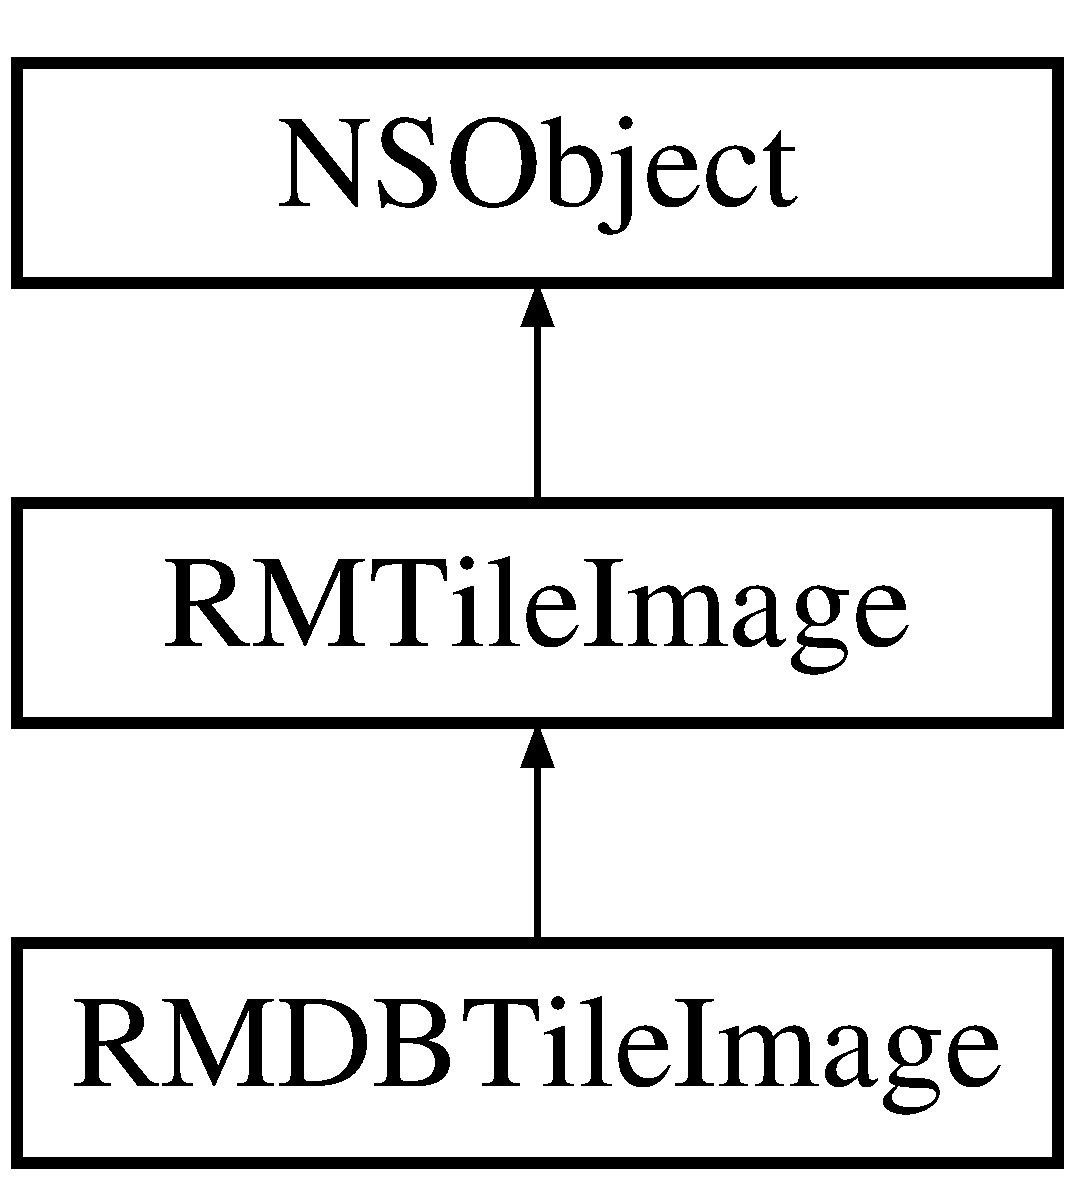
\includegraphics[height=3.000000cm]{interface_r_m_d_b_tile_image}
\end{center}
\end{figure}
\subsection*{Instance Methods}
\begin{DoxyCompactItemize}
\item 
(id) -\/ \hyperlink{interface_r_m_d_b_tile_image_a701b3ad8c92055426983ec1f29624e4e}{init\-With\-Tile\-:from\-D\-B\-:}
\end{DoxyCompactItemize}
\subsection*{额外继承的成员函数}


\subsection{Method Documentation}
\hypertarget{interface_r_m_d_b_tile_image_a701b3ad8c92055426983ec1f29624e4e}{\index{R\-M\-D\-B\-Tile\-Image@{R\-M\-D\-B\-Tile\-Image}!init\-With\-Tile\-:from\-D\-B\-:@{init\-With\-Tile\-:from\-D\-B\-:}}
\index{init\-With\-Tile\-:from\-D\-B\-:@{init\-With\-Tile\-:from\-D\-B\-:}!RMDBTileImage@{R\-M\-D\-B\-Tile\-Image}}
\subsubsection[{init\-With\-Tile\-:from\-D\-B\-:}]{\setlength{\rightskip}{0pt plus 5cm}-\/ (id) {\bf init\-With\-Tile\-:} 
\begin{DoxyParamCaption}
\item[{({\bf R\-M\-Tile})}]{tile}
\item[{fromDB:(F\-M\-Database$\ast$)}]{db}
\end{DoxyParamCaption}
}}\label{interface_r_m_d_b_tile_image_a701b3ad8c92055426983ec1f29624e4e}


该类的文档由以下文件生成\-:\begin{DoxyCompactItemize}
\item 
Map/\hyperlink{_r_m_d_b_tile_image_8h}{R\-M\-D\-B\-Tile\-Image.\-h}\item 
Map/\hyperlink{_r_m_d_b_tile_image_8m}{R\-M\-D\-B\-Tile\-Image.\-m}\end{DoxyCompactItemize}

\hypertarget{interface_r_m_file_tile_image}{\section{R\-M\-File\-Tile\-Image类 参考}
\label{interface_r_m_file_tile_image}\index{R\-M\-File\-Tile\-Image@{R\-M\-File\-Tile\-Image}}
}


\hyperlink{interface_r_m_tile_image}{R\-M\-Tile\-Image} subclass\-: a tile image loaded from a local file.  




{\ttfamily \#import $<$R\-M\-File\-Tile\-Image.\-h$>$}

类 R\-M\-File\-Tile\-Image 继承关系图\-:\begin{figure}[H]
\begin{center}
\leavevmode
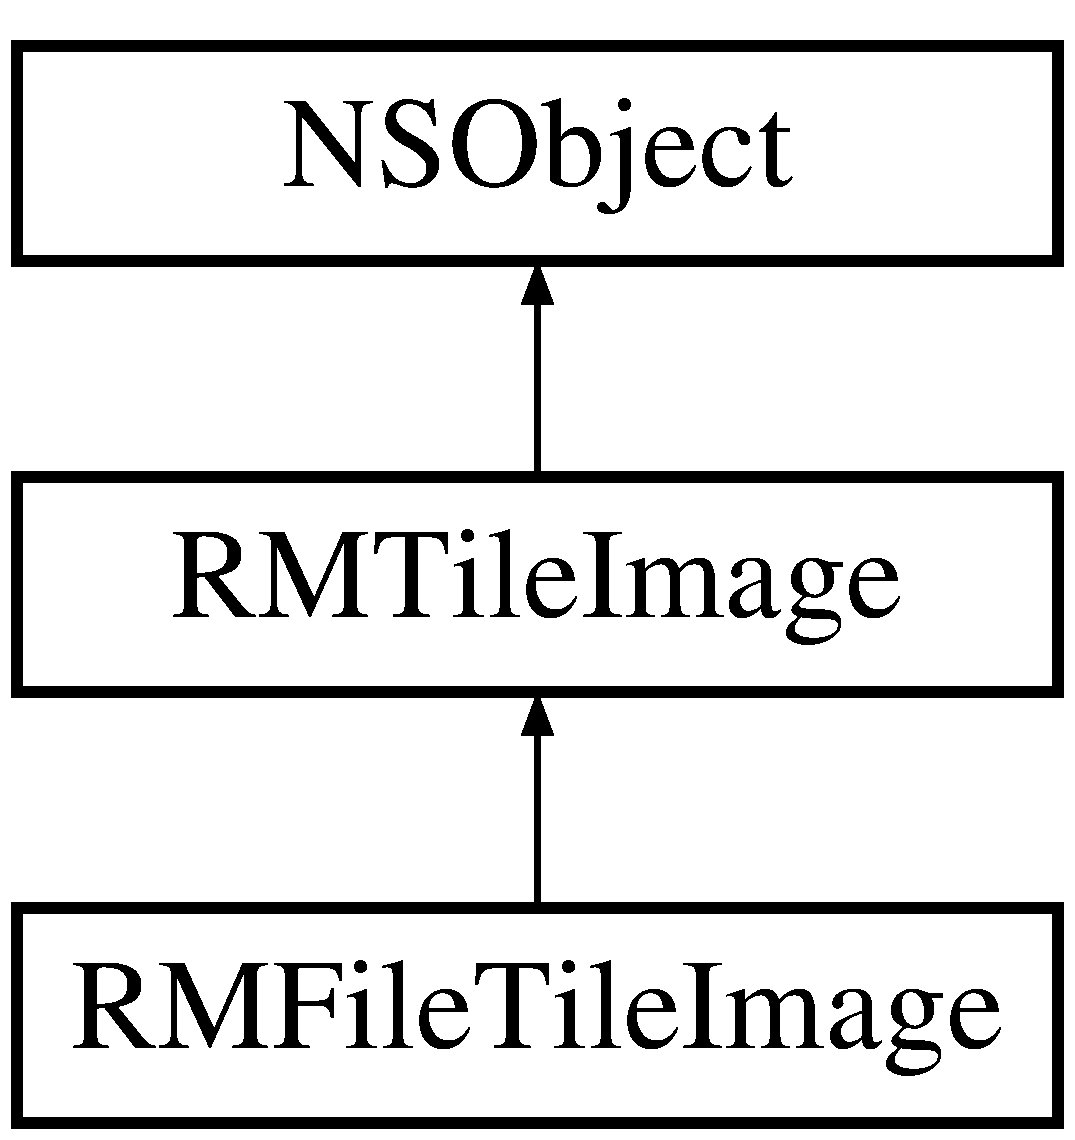
\includegraphics[height=3.000000cm]{interface_r_m_file_tile_image}
\end{center}
\end{figure}
\subsection*{Instance Methods}
\begin{DoxyCompactItemize}
\item 
(id) -\/ \hyperlink{interface_r_m_file_tile_image_a5acaf253522f8458c6fcebe3e6f71567}{init\-With\-Tile\-:\-From\-File\-:}
\end{DoxyCompactItemize}
\subsection*{额外继承的成员函数}


\subsection{详细描述}
\hyperlink{interface_r_m_tile_image}{R\-M\-Tile\-Image} subclass\-: a tile image loaded from a local file. 

\subsection{Method Documentation}
\hypertarget{interface_r_m_file_tile_image_a5acaf253522f8458c6fcebe3e6f71567}{\index{R\-M\-File\-Tile\-Image@{R\-M\-File\-Tile\-Image}!init\-With\-Tile\-:\-From\-File\-:@{init\-With\-Tile\-:\-From\-File\-:}}
\index{init\-With\-Tile\-:\-From\-File\-:@{init\-With\-Tile\-:\-From\-File\-:}!RMFileTileImage@{R\-M\-File\-Tile\-Image}}
\subsubsection[{init\-With\-Tile\-:\-From\-File\-:}]{\setlength{\rightskip}{0pt plus 5cm}-\/ (id) {\bf init\-With\-Tile\-:} 
\begin{DoxyParamCaption}
\item[{({\bf R\-M\-Tile})}]{\-\_\-tile}
\item[{FromFile:(N\-S\-String$\ast$)}]{filename}
\end{DoxyParamCaption}
}}\label{interface_r_m_file_tile_image_a5acaf253522f8458c6fcebe3e6f71567}


该类的文档由以下文件生成\-:\begin{DoxyCompactItemize}
\item 
Map/\hyperlink{_r_m_file_tile_image_8h}{R\-M\-File\-Tile\-Image.\-h}\item 
Map/\hyperlink{_r_m_file_tile_image_8m}{R\-M\-File\-Tile\-Image.\-m}\end{DoxyCompactItemize}

\hypertarget{interface_r_m_foundation_tests}{\section{R\-M\-Foundation\-Tests类 参考}
\label{interface_r_m_foundation_tests}\index{R\-M\-Foundation\-Tests@{R\-M\-Foundation\-Tests}}
}


{\ttfamily \#import $<$R\-M\-Foundation\-Tests.\-h$>$}

类 R\-M\-Foundation\-Tests 继承关系图\-:\begin{figure}[H]
\begin{center}
\leavevmode
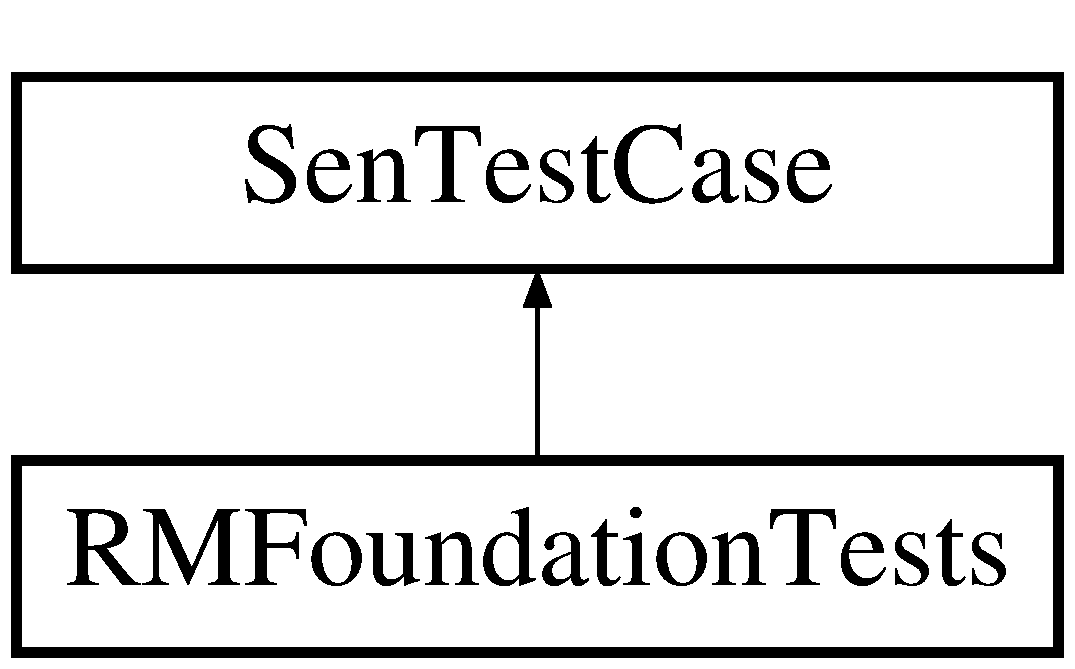
\includegraphics[height=2.000000cm]{interface_r_m_foundation_tests}
\end{center}
\end{figure}
\subsection*{Instance Methods}
\begin{DoxyCompactItemize}
\item 
(void) -\/ \hyperlink{interface_r_m_foundation_tests_a53d1f09166be8730acb142f56d26a336}{test\-Projected\-Rect\-Intersects\-Projected\-Rect}{\ttfamily  \mbox{[}implementation\mbox{]}}
\end{DoxyCompactItemize}


\subsection{Method Documentation}
\hypertarget{interface_r_m_foundation_tests_a53d1f09166be8730acb142f56d26a336}{\index{R\-M\-Foundation\-Tests@{R\-M\-Foundation\-Tests}!test\-Projected\-Rect\-Intersects\-Projected\-Rect@{test\-Projected\-Rect\-Intersects\-Projected\-Rect}}
\index{test\-Projected\-Rect\-Intersects\-Projected\-Rect@{test\-Projected\-Rect\-Intersects\-Projected\-Rect}!RMFoundationTests@{R\-M\-Foundation\-Tests}}
\subsubsection[{test\-Projected\-Rect\-Intersects\-Projected\-Rect}]{\setlength{\rightskip}{0pt plus 5cm}-\/ (void) test\-Projected\-Rect\-Intersects\-Projected\-Rect 
\begin{DoxyParamCaption}
{}
\end{DoxyParamCaption}
\hspace{0.3cm}{\ttfamily [implementation]}}}\label{interface_r_m_foundation_tests_a53d1f09166be8730acb142f56d26a336}


该类的文档由以下文件生成\-:\begin{DoxyCompactItemize}
\item 
\hyperlink{_r_m_foundation_tests_8h}{R\-M\-Foundation\-Tests.\-h}\item 
\hyperlink{_r_m_foundation_tests_8m}{R\-M\-Foundation\-Tests.\-m}\end{DoxyCompactItemize}

\hypertarget{interface_r_m_fractal_tile_projection}{\section{R\-M\-Fractal\-Tile\-Projection类 参考}
\label{interface_r_m_fractal_tile_projection}\index{R\-M\-Fractal\-Tile\-Projection@{R\-M\-Fractal\-Tile\-Projection}}
}


{\ttfamily \#import $<$R\-M\-Fractal\-Tile\-Projection.\-h$>$}

类 R\-M\-Fractal\-Tile\-Projection 继承关系图\-:\begin{figure}[H]
\begin{center}
\leavevmode
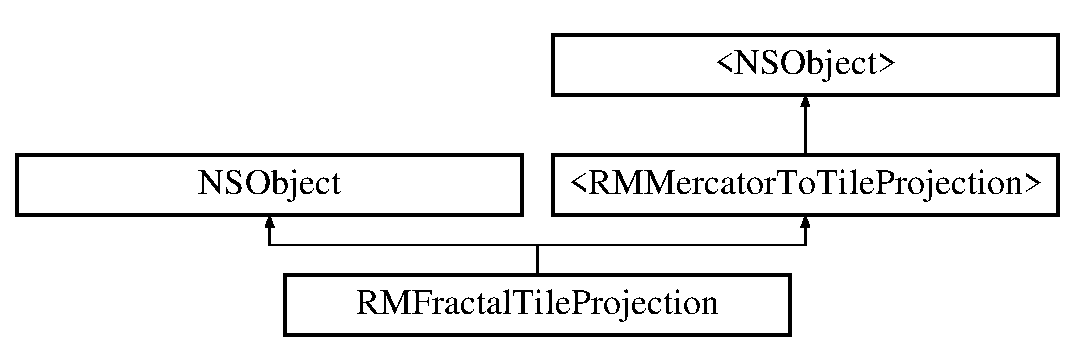
\includegraphics[height=3.000000cm]{interface_r_m_fractal_tile_projection}
\end{center}
\end{figure}
\subsection*{Instance Methods}
\begin{DoxyCompactItemize}
\item 
(float) -\/ \hyperlink{interface_r_m_fractal_tile_projection_a6432f229f4cfabfba65b7b702d0eb96c}{calculate\-Normalised\-Zoom\-From\-Scale\-:}{\ttfamily  \mbox{[}implementation\mbox{]}}
\item 
(float) -\/ \hyperlink{interface_r_m_fractal_tile_projection_aea5d9c0bdb2b6eb460d9882d6b2a46ec}{calculate\-Scale\-From\-Zoom\-:}{\ttfamily  \mbox{[}implementation\mbox{]}}
\item 
(float) -\/ \hyperlink{interface_r_m_fractal_tile_projection_a8604a8779fd50182367c0b176bd5a2ec}{calculate\-Zoom\-From\-Scale\-:}{\ttfamily  \mbox{[}implementation\mbox{]}}
\item 
(\hyperlink{struct_r_m_projected_point}{R\-M\-Projected\-Point}) -\/ \hyperlink{interface_r_m_fractal_tile_projection_a8e18cdf789364738340b838bf0638185}{constrain\-Point\-Horizontally\-:}{\ttfamily  \mbox{[}implementation\mbox{]}}
\item 
(id) -\/ \hyperlink{interface_r_m_fractal_tile_projection_af734f3ef032f0eacc03d35b3dc6dbbea}{init\-From\-Projection\-:tile\-Side\-Length\-:max\-Zoom\-:min\-Zoom\-:}
\item 
(float) -\/ \hyperlink{interface_r_m_fractal_tile_projection_abdf987db026c7761e2f57b0ea8207464}{limit\-From\-Normalised\-Zoom\-:}{\ttfamily  \mbox{[}implementation\mbox{]}}
\item 
(\hyperlink{struct_r_m_tile}{R\-M\-Tile}) -\/ \hyperlink{interface_r_m_fractal_tile_projection_a6ab9f21ef545dbac3647001f64022335}{normalise\-Tile\-:}{\ttfamily  \mbox{[}implementation\mbox{]}}
\item 
(float) -\/ \hyperlink{interface_r_m_fractal_tile_projection_a08e53c12b44631258e909dbc33385c96}{normalise\-Zoom\-:}{\ttfamily  \mbox{[}implementation\mbox{]}}
\item 
(\hyperlink{struct_r_m_tile_rect}{R\-M\-Tile\-Rect}) -\/ \hyperlink{interface_r_m_fractal_tile_projection_a76f6d1fea39a1c577ff0b26012b05c9c}{project\-:}{\ttfamily  \mbox{[}implementation\mbox{]}}
\begin{DoxyCompactList}\small\item\em This is a helper for project\-Rect above. Much simpler for the caller. \end{DoxyCompactList}\item 
(\hyperlink{struct_r_m_tile_point}{R\-M\-Tile\-Point}) -\/ \hyperlink{interface_r_m_fractal_tile_projection_a794c40f61be19f6efcb23e95a45ab1b4}{project\-:at\-Scale\-:}{\ttfamily  \mbox{[}implementation\mbox{]}}
\item 
(\hyperlink{struct_r_m_tile_point}{R\-M\-Tile\-Point}) -\/ \hyperlink{interface_r_m_fractal_tile_projection_afff85793493770d6424965f65c5690f7}{project\-:at\-Zoom\-:}{\ttfamily  \mbox{[}implementation\mbox{]}}
\item 
(\hyperlink{struct_r_m_tile_point}{R\-M\-Tile\-Point}) -\/ \hyperlink{interface_r_m_fractal_tile_projection_a955ae8a9935b4272437db0deb4e19869}{project\-Internal\-:normalised\-Zoom\-:limit\-:}{\ttfamily  \mbox{[}implementation\mbox{]}}
\item 
(\hyperlink{struct_r_m_tile_rect}{R\-M\-Tile\-Rect}) -\/ \hyperlink{interface_r_m_fractal_tile_projection_aca623bc1c542e85df15c30cfd2233b88}{project\-Rect\-:at\-Scale\-:}{\ttfamily  \mbox{[}implementation\mbox{]}}
\item 
(\hyperlink{struct_r_m_tile_rect}{R\-M\-Tile\-Rect}) -\/ \hyperlink{interface_r_m_fractal_tile_projection_abd518c9cae2d4440be0d00be14dff12b}{project\-Rect\-:at\-Zoom\-:}{\ttfamily  \mbox{[}implementation\mbox{]}}
\item 
(void) -\/ \hyperlink{interface_r_m_fractal_tile_projection_a1de5623a97b039eb67df69dd9b76cd7a}{set\-Max\-Zoom\-:}
\item 
(void) -\/ \hyperlink{interface_r_m_fractal_tile_projection_ac749932c5662241d26cbed5ecead0509}{set\-Min\-Zoom\-:}
\item 
(void) -\/ \hyperlink{interface_r_m_fractal_tile_projection_a14bce0b9cfa03a35c689e5b59ffd1129}{set\-Tile\-Side\-Length\-:}
\end{DoxyCompactItemize}
\subsection*{Protected 属性}
\begin{DoxyCompactItemize}
\item 
N\-S\-U\-Integer \hyperlink{interface_r_m_fractal_tile_projection_af46f235f561d62545f4c299cb22284ff}{max\-Zoom}
\begin{DoxyCompactList}\small\item\em Maximum zoom for which our tile server stores images. \end{DoxyCompactList}\item 
N\-S\-U\-Integer \hyperlink{interface_r_m_fractal_tile_projection_a17ca1a6850b0adc8c1838a88322e8cb6}{min\-Zoom}
\item 
\hyperlink{struct_r_m_projected_rect}{R\-M\-Projected\-Rect} \hyperlink{interface_r_m_fractal_tile_projection_a5f3e841cee4a8573bfc60a6ec8a35884}{planet\-Bounds}
\begin{DoxyCompactList}\small\item\em projected bounds of the planet, in meters \end{DoxyCompactList}\item 
double \hyperlink{interface_r_m_fractal_tile_projection_a297753455c83bc2d681dad601fb7a9c5}{scale\-Factor}
\begin{DoxyCompactList}\small\item\em The deal is, we have a scale which stores how many mercator gradiants per pixel in the image. \end{DoxyCompactList}\item 
N\-S\-U\-Integer \hyperlink{interface_r_m_fractal_tile_projection_ad84192b0999b267f8fbccd827eeab01e}{tile\-Side\-Length}
\begin{DoxyCompactList}\small\item\em Normally 256. This class assumes tiles are square. \end{DoxyCompactList}\end{DoxyCompactItemize}
\subsection*{额外继承的成员函数}


\subsection{Method Documentation}
\hypertarget{interface_r_m_fractal_tile_projection_a6432f229f4cfabfba65b7b702d0eb96c}{\index{R\-M\-Fractal\-Tile\-Projection@{R\-M\-Fractal\-Tile\-Projection}!calculate\-Normalised\-Zoom\-From\-Scale\-:@{calculate\-Normalised\-Zoom\-From\-Scale\-:}}
\index{calculate\-Normalised\-Zoom\-From\-Scale\-:@{calculate\-Normalised\-Zoom\-From\-Scale\-:}!RMFractalTileProjection@{R\-M\-Fractal\-Tile\-Projection}}
\subsubsection[{calculate\-Normalised\-Zoom\-From\-Scale\-:}]{\setlength{\rightskip}{0pt plus 5cm}-\/ (float) calculate\-Normalised\-Zoom\-From\-Scale\-: 
\begin{DoxyParamCaption}
\item[{(float)}]{scale}
\end{DoxyParamCaption}
\hspace{0.3cm}{\ttfamily [implementation]}}}\label{interface_r_m_fractal_tile_projection_a6432f229f4cfabfba65b7b702d0eb96c}


重载 \hyperlink{protocol_r_m_mercator_to_tile_projection-p_a470b0ea952dd174bbd573bdfb230cc6e}{$<$\-R\-M\-Mercator\-To\-Tile\-Projection$>$} .

\hypertarget{interface_r_m_fractal_tile_projection_aea5d9c0bdb2b6eb460d9882d6b2a46ec}{\index{R\-M\-Fractal\-Tile\-Projection@{R\-M\-Fractal\-Tile\-Projection}!calculate\-Scale\-From\-Zoom\-:@{calculate\-Scale\-From\-Zoom\-:}}
\index{calculate\-Scale\-From\-Zoom\-:@{calculate\-Scale\-From\-Zoom\-:}!RMFractalTileProjection@{R\-M\-Fractal\-Tile\-Projection}}
\subsubsection[{calculate\-Scale\-From\-Zoom\-:}]{\setlength{\rightskip}{0pt plus 5cm}-\/ (float) calculate\-Scale\-From\-Zoom\-: 
\begin{DoxyParamCaption}
\item[{(float)}]{zoom}
\end{DoxyParamCaption}
\hspace{0.3cm}{\ttfamily [implementation]}}}\label{interface_r_m_fractal_tile_projection_aea5d9c0bdb2b6eb460d9882d6b2a46ec}


重载 \hyperlink{protocol_r_m_mercator_to_tile_projection-p_a49c836acfac1908808c5f218f3bc64a4}{$<$\-R\-M\-Mercator\-To\-Tile\-Projection$>$} .

\hypertarget{interface_r_m_fractal_tile_projection_a8604a8779fd50182367c0b176bd5a2ec}{\index{R\-M\-Fractal\-Tile\-Projection@{R\-M\-Fractal\-Tile\-Projection}!calculate\-Zoom\-From\-Scale\-:@{calculate\-Zoom\-From\-Scale\-:}}
\index{calculate\-Zoom\-From\-Scale\-:@{calculate\-Zoom\-From\-Scale\-:}!RMFractalTileProjection@{R\-M\-Fractal\-Tile\-Projection}}
\subsubsection[{calculate\-Zoom\-From\-Scale\-:}]{\setlength{\rightskip}{0pt plus 5cm}-\/ (float) calculate\-Zoom\-From\-Scale\-: 
\begin{DoxyParamCaption}
\item[{(float)}]{scale}
\end{DoxyParamCaption}
\hspace{0.3cm}{\ttfamily [implementation]}}}\label{interface_r_m_fractal_tile_projection_a8604a8779fd50182367c0b176bd5a2ec}


重载 \hyperlink{protocol_r_m_mercator_to_tile_projection-p_a013a65cf254c34e3ec021864a4fb8f53}{$<$\-R\-M\-Mercator\-To\-Tile\-Projection$>$} .



参考自 calculate\-Normalised\-Zoom\-From\-Scale\-:, project\-:at\-Scale\-: , 以及 project\-Rect\-:at\-Scale\-:.

\hypertarget{interface_r_m_fractal_tile_projection_a8e18cdf789364738340b838bf0638185}{\index{R\-M\-Fractal\-Tile\-Projection@{R\-M\-Fractal\-Tile\-Projection}!constrain\-Point\-Horizontally\-:@{constrain\-Point\-Horizontally\-:}}
\index{constrain\-Point\-Horizontally\-:@{constrain\-Point\-Horizontally\-:}!RMFractalTileProjection@{R\-M\-Fractal\-Tile\-Projection}}
\subsubsection[{constrain\-Point\-Horizontally\-:}]{\setlength{\rightskip}{0pt plus 5cm}-\/ ({\bf R\-M\-Projected\-Point}) constrain\-Point\-Horizontally\-: 
\begin{DoxyParamCaption}
\item[{({\bf R\-M\-Projected\-Point})}]{a\-Point}
\end{DoxyParamCaption}
\hspace{0.3cm}{\ttfamily [implementation]}}}\label{interface_r_m_fractal_tile_projection_a8e18cdf789364738340b838bf0638185}


参考自 project\-Internal\-:normalised\-Zoom\-:limit\-:.

\hypertarget{interface_r_m_fractal_tile_projection_af734f3ef032f0eacc03d35b3dc6dbbea}{\index{R\-M\-Fractal\-Tile\-Projection@{R\-M\-Fractal\-Tile\-Projection}!init\-From\-Projection\-:tile\-Side\-Length\-:max\-Zoom\-:min\-Zoom\-:@{init\-From\-Projection\-:tile\-Side\-Length\-:max\-Zoom\-:min\-Zoom\-:}}
\index{init\-From\-Projection\-:tile\-Side\-Length\-:max\-Zoom\-:min\-Zoom\-:@{init\-From\-Projection\-:tile\-Side\-Length\-:max\-Zoom\-:min\-Zoom\-:}!RMFractalTileProjection@{R\-M\-Fractal\-Tile\-Projection}}
\subsubsection[{init\-From\-Projection\-:tile\-Side\-Length\-:max\-Zoom\-:min\-Zoom\-:}]{\setlength{\rightskip}{0pt plus 5cm}-\/ (id) init\-From\-Projection\-: 
\begin{DoxyParamCaption}
\item[{({\bf R\-M\-Projection}$\ast$)}]{projection}
\item[{tileSideLength:(N\-S\-U\-Integer)}]{tile\-Side\-Length}
\item[{maxZoom:(N\-S\-U\-Integer)}]{a\-Max\-Zoom}
\item[{minZoom:(N\-S\-U\-Integer)}]{a\-Min\-Zoom}
\end{DoxyParamCaption}
}}\label{interface_r_m_fractal_tile_projection_af734f3ef032f0eacc03d35b3dc6dbbea}
\begin{DoxyRefDesc}{Bug}
\item[\hyperlink{bug__bug000007}{Bug}]magic string literals \end{DoxyRefDesc}
\hypertarget{interface_r_m_fractal_tile_projection_abdf987db026c7761e2f57b0ea8207464}{\index{R\-M\-Fractal\-Tile\-Projection@{R\-M\-Fractal\-Tile\-Projection}!limit\-From\-Normalised\-Zoom\-:@{limit\-From\-Normalised\-Zoom\-:}}
\index{limit\-From\-Normalised\-Zoom\-:@{limit\-From\-Normalised\-Zoom\-:}!RMFractalTileProjection@{R\-M\-Fractal\-Tile\-Projection}}
\subsubsection[{limit\-From\-Normalised\-Zoom\-:}]{\setlength{\rightskip}{0pt plus 5cm}-\/ (float) limit\-From\-Normalised\-Zoom\-: 
\begin{DoxyParamCaption}
\item[{(float)}]{zoom}
\end{DoxyParamCaption}
\hspace{0.3cm}{\ttfamily [implementation]}}}\label{interface_r_m_fractal_tile_projection_abdf987db026c7761e2f57b0ea8207464}


参考自 project\-:at\-Zoom\-: , 以及 project\-Rect\-:at\-Zoom\-:.

\hypertarget{interface_r_m_fractal_tile_projection_a6ab9f21ef545dbac3647001f64022335}{\index{R\-M\-Fractal\-Tile\-Projection@{R\-M\-Fractal\-Tile\-Projection}!normalise\-Tile\-:@{normalise\-Tile\-:}}
\index{normalise\-Tile\-:@{normalise\-Tile\-:}!RMFractalTileProjection@{R\-M\-Fractal\-Tile\-Projection}}
\subsubsection[{normalise\-Tile\-:}]{\setlength{\rightskip}{0pt plus 5cm}-\/ ({\bf R\-M\-Tile}) normalise\-Tile\-: 
\begin{DoxyParamCaption}
\item[{({\bf R\-M\-Tile})}]{tile}
\end{DoxyParamCaption}
\hspace{0.3cm}{\ttfamily [implementation]}}}\label{interface_r_m_fractal_tile_projection_a6ab9f21ef545dbac3647001f64022335}


重载 \hyperlink{protocol_r_m_mercator_to_tile_projection-p_ac8776965edc17be3e90c03aad46a8371}{$<$\-R\-M\-Mercator\-To\-Tile\-Projection$>$} .



参考自 R\-M\-Abstract\-Mercator\-Web\-Source\-::tile\-Image\-: , 以及 R\-M\-D\-B\-Map\-Source\-::tile\-Image\-:.

\hypertarget{interface_r_m_fractal_tile_projection_a08e53c12b44631258e909dbc33385c96}{\index{R\-M\-Fractal\-Tile\-Projection@{R\-M\-Fractal\-Tile\-Projection}!normalise\-Zoom\-:@{normalise\-Zoom\-:}}
\index{normalise\-Zoom\-:@{normalise\-Zoom\-:}!RMFractalTileProjection@{R\-M\-Fractal\-Tile\-Projection}}
\subsubsection[{normalise\-Zoom\-:}]{\setlength{\rightskip}{0pt plus 5cm}-\/ (float) normalise\-Zoom\-: 
\begin{DoxyParamCaption}
\item[{(float)}]{zoom}
\end{DoxyParamCaption}
\hspace{0.3cm}{\ttfamily [implementation]}}}\label{interface_r_m_fractal_tile_projection_a08e53c12b44631258e909dbc33385c96}


重载 \hyperlink{protocol_r_m_mercator_to_tile_projection-p_a48d47f3689db59a82bde9da209529f9b}{$<$\-R\-M\-Mercator\-To\-Tile\-Projection$>$} .



参考自 calculate\-Normalised\-Zoom\-From\-Scale\-:, project\-:at\-Zoom\-: , 以及 project\-Rect\-:at\-Zoom\-:.

\hypertarget{interface_r_m_fractal_tile_projection_a76f6d1fea39a1c577ff0b26012b05c9c}{\index{R\-M\-Fractal\-Tile\-Projection@{R\-M\-Fractal\-Tile\-Projection}!project\-:@{project\-:}}
\index{project\-:@{project\-:}!RMFractalTileProjection@{R\-M\-Fractal\-Tile\-Projection}}
\subsubsection[{project\-:}]{\setlength{\rightskip}{0pt plus 5cm}-\/ ({\bf R\-M\-Tile\-Rect}) project\-: 
\begin{DoxyParamCaption}
\item[{({\bf R\-M\-Mercator\-To\-Screen\-Projection} $\ast$)}]{screen}
\end{DoxyParamCaption}
\hspace{0.3cm}{\ttfamily [implementation]}}}\label{interface_r_m_fractal_tile_projection_a76f6d1fea39a1c577ff0b26012b05c9c}


This is a helper for project\-Rect above. Much simpler for the caller. 



重载 \hyperlink{protocol_r_m_mercator_to_tile_projection-p_ae80633ea6d0b4e354666ec6e7ddd88af}{$<$\-R\-M\-Mercator\-To\-Tile\-Projection$>$} .

\hypertarget{interface_r_m_fractal_tile_projection_a794c40f61be19f6efcb23e95a45ab1b4}{\index{R\-M\-Fractal\-Tile\-Projection@{R\-M\-Fractal\-Tile\-Projection}!project\-:at\-Scale\-:@{project\-:at\-Scale\-:}}
\index{project\-:at\-Scale\-:@{project\-:at\-Scale\-:}!RMFractalTileProjection@{R\-M\-Fractal\-Tile\-Projection}}
\subsubsection[{project\-:at\-Scale\-:}]{\setlength{\rightskip}{0pt plus 5cm}-\/ ({\bf R\-M\-Tile\-Point}) {\bf project\-:} 
\begin{DoxyParamCaption}
\item[{({\bf R\-M\-Projected\-Point})}]{a\-Point}
\item[{atScale:(float)}]{scale}
\end{DoxyParamCaption}
\hspace{0.3cm}{\ttfamily [implementation]}}}\label{interface_r_m_fractal_tile_projection_a794c40f61be19f6efcb23e95a45ab1b4}


重载 \hyperlink{protocol_r_m_mercator_to_tile_projection-p_aac47d8222bec29f9d8469d166510b9cd}{$<$\-R\-M\-Mercator\-To\-Tile\-Projection$>$} .

\hypertarget{interface_r_m_fractal_tile_projection_afff85793493770d6424965f65c5690f7}{\index{R\-M\-Fractal\-Tile\-Projection@{R\-M\-Fractal\-Tile\-Projection}!project\-:at\-Zoom\-:@{project\-:at\-Zoom\-:}}
\index{project\-:at\-Zoom\-:@{project\-:at\-Zoom\-:}!RMFractalTileProjection@{R\-M\-Fractal\-Tile\-Projection}}
\subsubsection[{project\-:at\-Zoom\-:}]{\setlength{\rightskip}{0pt plus 5cm}-\/ ({\bf R\-M\-Tile\-Point}) {\bf project\-:} 
\begin{DoxyParamCaption}
\item[{({\bf R\-M\-Projected\-Point})}]{a\-Point}
\item[{atZoom:(float)}]{zoom}
\end{DoxyParamCaption}
\hspace{0.3cm}{\ttfamily [implementation]}}}\label{interface_r_m_fractal_tile_projection_afff85793493770d6424965f65c5690f7}


重载 \hyperlink{protocol_r_m_mercator_to_tile_projection-p_a0351c94bf59dfc97b5c1c712a5b2f3b2}{$<$\-R\-M\-Mercator\-To\-Tile\-Projection$>$} .



参考自 project\-:at\-Scale\-:.

\hypertarget{interface_r_m_fractal_tile_projection_a955ae8a9935b4272437db0deb4e19869}{\index{R\-M\-Fractal\-Tile\-Projection@{R\-M\-Fractal\-Tile\-Projection}!project\-Internal\-:normalised\-Zoom\-:limit\-:@{project\-Internal\-:normalised\-Zoom\-:limit\-:}}
\index{project\-Internal\-:normalised\-Zoom\-:limit\-:@{project\-Internal\-:normalised\-Zoom\-:limit\-:}!RMFractalTileProjection@{R\-M\-Fractal\-Tile\-Projection}}
\subsubsection[{project\-Internal\-:normalised\-Zoom\-:limit\-:}]{\setlength{\rightskip}{0pt plus 5cm}-\/ ({\bf R\-M\-Tile\-Point}) project\-Internal\-: 
\begin{DoxyParamCaption}
\item[{({\bf R\-M\-Projected\-Point})}]{a\-Point}
\item[{normalisedZoom:(float)}]{zoom}
\item[{limit:(float)}]{limit}
\end{DoxyParamCaption}
\hspace{0.3cm}{\ttfamily [implementation]}}}\label{interface_r_m_fractal_tile_projection_a955ae8a9935b4272437db0deb4e19869}


参考自 project\-:at\-Zoom\-: , 以及 project\-Rect\-:at\-Zoom\-:.

\hypertarget{interface_r_m_fractal_tile_projection_aca623bc1c542e85df15c30cfd2233b88}{\index{R\-M\-Fractal\-Tile\-Projection@{R\-M\-Fractal\-Tile\-Projection}!project\-Rect\-:at\-Scale\-:@{project\-Rect\-:at\-Scale\-:}}
\index{project\-Rect\-:at\-Scale\-:@{project\-Rect\-:at\-Scale\-:}!RMFractalTileProjection@{R\-M\-Fractal\-Tile\-Projection}}
\subsubsection[{project\-Rect\-:at\-Scale\-:}]{\setlength{\rightskip}{0pt plus 5cm}-\/ ({\bf R\-M\-Tile\-Rect}) project\-Rect\-: 
\begin{DoxyParamCaption}
\item[{({\bf R\-M\-Projected\-Rect})}]{a\-Rect}
\item[{atScale:(float)}]{scale}
\end{DoxyParamCaption}
\hspace{0.3cm}{\ttfamily [implementation]}}}\label{interface_r_m_fractal_tile_projection_aca623bc1c542e85df15c30cfd2233b88}


重载 \hyperlink{protocol_r_m_mercator_to_tile_projection-p_a6d26aef35f64a793066fdf8c4e3cda10}{$<$\-R\-M\-Mercator\-To\-Tile\-Projection$>$} .



参考自 project\-:.

\hypertarget{interface_r_m_fractal_tile_projection_abd518c9cae2d4440be0d00be14dff12b}{\index{R\-M\-Fractal\-Tile\-Projection@{R\-M\-Fractal\-Tile\-Projection}!project\-Rect\-:at\-Zoom\-:@{project\-Rect\-:at\-Zoom\-:}}
\index{project\-Rect\-:at\-Zoom\-:@{project\-Rect\-:at\-Zoom\-:}!RMFractalTileProjection@{R\-M\-Fractal\-Tile\-Projection}}
\subsubsection[{project\-Rect\-:at\-Zoom\-:}]{\setlength{\rightskip}{0pt plus 5cm}-\/ ({\bf R\-M\-Tile\-Rect}) project\-Rect\-: 
\begin{DoxyParamCaption}
\item[{({\bf R\-M\-Projected\-Rect})}]{a\-Rect}
\item[{atZoom:(float)}]{zoom}
\end{DoxyParamCaption}
\hspace{0.3cm}{\ttfamily [implementation]}}}\label{interface_r_m_fractal_tile_projection_abd518c9cae2d4440be0d00be14dff12b}
\begin{DoxyRefDesc}{Bug}
\item[\hyperlink{bug__bug000008}{Bug}]assignment of float to int, W\-T\-F? \end{DoxyRefDesc}


重载 \hyperlink{protocol_r_m_mercator_to_tile_projection-p_a53c5b90994528d20a3d85307244ac412}{$<$\-R\-M\-Mercator\-To\-Tile\-Projection$>$} .



参考自 project\-Rect\-:at\-Scale\-:.

\hypertarget{interface_r_m_fractal_tile_projection_a1de5623a97b039eb67df69dd9b76cd7a}{\index{R\-M\-Fractal\-Tile\-Projection@{R\-M\-Fractal\-Tile\-Projection}!set\-Max\-Zoom\-:@{set\-Max\-Zoom\-:}}
\index{set\-Max\-Zoom\-:@{set\-Max\-Zoom\-:}!RMFractalTileProjection@{R\-M\-Fractal\-Tile\-Projection}}
\subsubsection[{set\-Max\-Zoom\-:}]{\setlength{\rightskip}{0pt plus 5cm}-\/ (void) set\-Max\-Zoom\-: 
\begin{DoxyParamCaption}
\item[{(N\-S\-U\-Integer)}]{a\-Max\-Zoom}
\end{DoxyParamCaption}
}}\label{interface_r_m_fractal_tile_projection_a1de5623a97b039eb67df69dd9b76cd7a}


参考自 R\-M\-Abstract\-Mercator\-Web\-Source\-::set\-Max\-Zoom\-:, R\-M\-D\-B\-Map\-Source\-::set\-Max\-Zoom\-: , 以及 R\-M\-M\-B\-Tiles\-Tile\-Source\-::set\-Max\-Zoom\-:.

\hypertarget{interface_r_m_fractal_tile_projection_ac749932c5662241d26cbed5ecead0509}{\index{R\-M\-Fractal\-Tile\-Projection@{R\-M\-Fractal\-Tile\-Projection}!set\-Min\-Zoom\-:@{set\-Min\-Zoom\-:}}
\index{set\-Min\-Zoom\-:@{set\-Min\-Zoom\-:}!RMFractalTileProjection@{R\-M\-Fractal\-Tile\-Projection}}
\subsubsection[{set\-Min\-Zoom\-:}]{\setlength{\rightskip}{0pt plus 5cm}-\/ (void) set\-Min\-Zoom\-: 
\begin{DoxyParamCaption}
\item[{(N\-S\-U\-Integer)}]{a\-Min\-Zoom}
\end{DoxyParamCaption}
}}\label{interface_r_m_fractal_tile_projection_ac749932c5662241d26cbed5ecead0509}


参考自 R\-M\-Abstract\-Mercator\-Web\-Source\-::set\-Min\-Zoom\-:, R\-M\-D\-B\-Map\-Source\-::set\-Min\-Zoom\-: , 以及 R\-M\-M\-B\-Tiles\-Tile\-Source\-::set\-Min\-Zoom\-:.

\hypertarget{interface_r_m_fractal_tile_projection_a14bce0b9cfa03a35c689e5b59ffd1129}{\index{R\-M\-Fractal\-Tile\-Projection@{R\-M\-Fractal\-Tile\-Projection}!set\-Tile\-Side\-Length\-:@{set\-Tile\-Side\-Length\-:}}
\index{set\-Tile\-Side\-Length\-:@{set\-Tile\-Side\-Length\-:}!RMFractalTileProjection@{R\-M\-Fractal\-Tile\-Projection}}
\subsubsection[{set\-Tile\-Side\-Length\-:}]{\setlength{\rightskip}{0pt plus 5cm}-\/ (void) set\-Tile\-Side\-Length\-: 
\begin{DoxyParamCaption}
\item[{(N\-S\-U\-Integer)}]{a\-Tile\-Side\-Length}
\end{DoxyParamCaption}
}}\label{interface_r_m_fractal_tile_projection_a14bce0b9cfa03a35c689e5b59ffd1129}


参考自 R\-M\-Abstract\-Mercator\-Web\-Source\-::set\-Tile\-Side\-Length\-: , 以及 R\-M\-M\-B\-Tiles\-Tile\-Source\-::set\-Tile\-Side\-Length\-:.



\subsection{类成员变量说明}
\hypertarget{interface_r_m_fractal_tile_projection_af46f235f561d62545f4c299cb22284ff}{\index{R\-M\-Fractal\-Tile\-Projection@{R\-M\-Fractal\-Tile\-Projection}!max\-Zoom@{max\-Zoom}}
\index{max\-Zoom@{max\-Zoom}!RMFractalTileProjection@{R\-M\-Fractal\-Tile\-Projection}}
\subsubsection[{max\-Zoom}]{\setlength{\rightskip}{0pt plus 5cm}-\/ (N\-S\-U\-Integer) max\-Zoom\hspace{0.3cm}{\ttfamily [protected]}}}\label{interface_r_m_fractal_tile_projection_af46f235f561d62545f4c299cb22284ff}


Maximum zoom for which our tile server stores images. 



参考自 init\-From\-Projection\-:tile\-Side\-Length\-:max\-Zoom\-:min\-Zoom\-:, R\-M\-Tiled\-Layer\-Controller\-::init\-With\-Tile\-Source\-:, R\-M\-Abstract\-Mercator\-Web\-Source\-::max\-Zoom, normalise\-Zoom\-: , 以及 set\-Max\-Zoom\-:.

\hypertarget{interface_r_m_fractal_tile_projection_a17ca1a6850b0adc8c1838a88322e8cb6}{\index{R\-M\-Fractal\-Tile\-Projection@{R\-M\-Fractal\-Tile\-Projection}!min\-Zoom@{min\-Zoom}}
\index{min\-Zoom@{min\-Zoom}!RMFractalTileProjection@{R\-M\-Fractal\-Tile\-Projection}}
\subsubsection[{min\-Zoom}]{\setlength{\rightskip}{0pt plus 5cm}-\/ (N\-S\-U\-Integer) min\-Zoom\hspace{0.3cm}{\ttfamily [protected]}}}\label{interface_r_m_fractal_tile_projection_a17ca1a6850b0adc8c1838a88322e8cb6}


参考自 init\-From\-Projection\-:tile\-Side\-Length\-:max\-Zoom\-:min\-Zoom\-:, R\-M\-Abstract\-Mercator\-Web\-Source\-::min\-Zoom, normalise\-Zoom\-: , 以及 set\-Min\-Zoom\-:.

\hypertarget{interface_r_m_fractal_tile_projection_a5f3e841cee4a8573bfc60a6ec8a35884}{\index{R\-M\-Fractal\-Tile\-Projection@{R\-M\-Fractal\-Tile\-Projection}!planet\-Bounds@{planet\-Bounds}}
\index{planet\-Bounds@{planet\-Bounds}!RMFractalTileProjection@{R\-M\-Fractal\-Tile\-Projection}}
\subsubsection[{planet\-Bounds}]{\setlength{\rightskip}{0pt plus 5cm}-\/ ({\bf R\-M\-Projected\-Rect}) planet\-Bounds\hspace{0.3cm}{\ttfamily [protected]}}}\label{interface_r_m_fractal_tile_projection_a5f3e841cee4a8573bfc60a6ec8a35884}


projected bounds of the planet, in meters 



参考自 calculate\-Scale\-From\-Zoom\-:, constrain\-Point\-Horizontally\-:, init\-From\-Projection\-:tile\-Side\-Length\-:max\-Zoom\-:min\-Zoom\-:, project\-Internal\-:normalised\-Zoom\-:limit\-:, project\-Rect\-:at\-Zoom\-: , 以及 set\-Tile\-Side\-Length\-:.

\hypertarget{interface_r_m_fractal_tile_projection_a297753455c83bc2d681dad601fb7a9c5}{\index{R\-M\-Fractal\-Tile\-Projection@{R\-M\-Fractal\-Tile\-Projection}!scale\-Factor@{scale\-Factor}}
\index{scale\-Factor@{scale\-Factor}!RMFractalTileProjection@{R\-M\-Fractal\-Tile\-Projection}}
\subsubsection[{scale\-Factor}]{\setlength{\rightskip}{0pt plus 5cm}-\/ (double) scale\-Factor\hspace{0.3cm}{\ttfamily [protected]}}}\label{interface_r_m_fractal_tile_projection_a297753455c83bc2d681dad601fb7a9c5}


The deal is, we have a scale which stores how many mercator gradiants per pixel in the image. 

If you run the maths, scale = bounds.\-width/(2$^\wedge$zoom $\ast$ tile\-Side\-Length) or if you want, z = log(bounds.\-width/tile\-Side\-Length) -\/ log(s) So here we'll cache the first term for efficiency. I'm using width arbitrarily -\/ I'm not sure what the effect of using the other term is when they're not the same. 

参考自 calculate\-Zoom\-From\-Scale\-:, init\-From\-Projection\-:tile\-Side\-Length\-:max\-Zoom\-:min\-Zoom\-: , 以及 set\-Tile\-Side\-Length\-:.

\hypertarget{interface_r_m_fractal_tile_projection_ad84192b0999b267f8fbccd827eeab01e}{\index{R\-M\-Fractal\-Tile\-Projection@{R\-M\-Fractal\-Tile\-Projection}!tile\-Side\-Length@{tile\-Side\-Length}}
\index{tile\-Side\-Length@{tile\-Side\-Length}!RMFractalTileProjection@{R\-M\-Fractal\-Tile\-Projection}}
\subsubsection[{tile\-Side\-Length}]{\setlength{\rightskip}{0pt plus 5cm}-\/ (N\-S\-U\-Integer) tile\-Side\-Length\hspace{0.3cm}{\ttfamily [protected]}}}\label{interface_r_m_fractal_tile_projection_ad84192b0999b267f8fbccd827eeab01e}


Normally 256. This class assumes tiles are square. 



参考自 calculate\-Scale\-From\-Zoom\-:, init\-From\-Projection\-:tile\-Side\-Length\-:max\-Zoom\-:min\-Zoom\-:, R\-M\-Tiled\-Layer\-Controller\-::init\-With\-Tile\-Source\-:, set\-Tile\-Side\-Length\-:, R\-M\-Abstract\-Mercator\-Web\-Source\-::tile\-Side\-Length , 以及 R\-M\-M\-B\-Tiles\-Tile\-Source\-::tile\-Side\-Length.



该类的文档由以下文件生成\-:\begin{DoxyCompactItemize}
\item 
Map/\hyperlink{_r_m_fractal_tile_projection_8h}{R\-M\-Fractal\-Tile\-Projection.\-h}\item 
Map/\hyperlink{_r_m_fractal_tile_projection_8m}{R\-M\-Fractal\-Tile\-Projection.\-m}\end{DoxyCompactItemize}

\hypertarget{interface_r_m_geo_hash}{\section{R\-M\-Geo\-Hash类 参考}
\label{interface_r_m_geo_hash}\index{R\-M\-Geo\-Hash@{R\-M\-Geo\-Hash}}
}


{\ttfamily \#import $<$R\-M\-Geo\-Hash.\-h$>$}

类 R\-M\-Geo\-Hash 继承关系图\-:\begin{figure}[H]
\begin{center}
\leavevmode
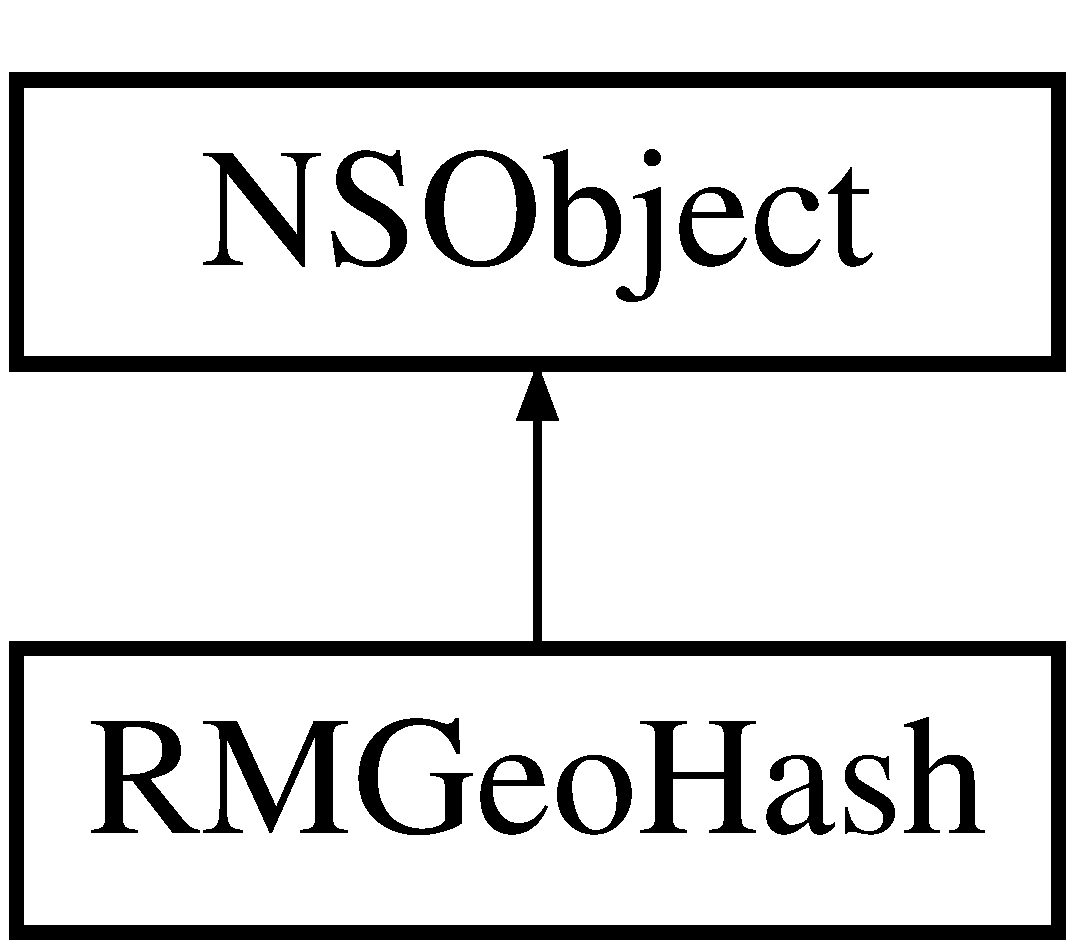
\includegraphics[height=2.000000cm]{interface_r_m_geo_hash}
\end{center}
\end{figure}
\subsection*{Class Methods}
\begin{DoxyCompactItemize}
\item 
(N\-S\-String $\ast$) + \hyperlink{interface_r_m_geo_hash_a86e1173157e7b7c767a99d7600271089}{adjacent\-Of\-:in\-Dir\-:}
\item 
(void) + \hyperlink{interface_r_m_geo_hash_a6ba74566179515b05aa27d5fc6a11cda}{convert\-:to\-Min\-:max\-:}
\item 
(N\-S\-String $\ast$) + \hyperlink{interface_r_m_geo_hash_a5960f23d79730f699cddd5318085f84c}{from\-Location\-:with\-Precision\-:}
\item 
(N\-S\-Array $\ast$) + \hyperlink{interface_r_m_geo_hash_a8f8f1993f25b618665202cd5539fffc8}{with\-Neighbors\-:}
\end{DoxyCompactItemize}


\subsection{Method Documentation}
\hypertarget{interface_r_m_geo_hash_a86e1173157e7b7c767a99d7600271089}{\index{R\-M\-Geo\-Hash@{R\-M\-Geo\-Hash}!adjacent\-Of\-:in\-Dir\-:@{adjacent\-Of\-:in\-Dir\-:}}
\index{adjacent\-Of\-:in\-Dir\-:@{adjacent\-Of\-:in\-Dir\-:}!RMGeoHash@{R\-M\-Geo\-Hash}}
\subsubsection[{adjacent\-Of\-:in\-Dir\-:}]{\setlength{\rightskip}{0pt plus 5cm}+ (N\-S\-String $\ast$) adjacent\-Of\-: 
\begin{DoxyParamCaption}
\item[{(N\-S\-String $\ast$)}]{src\-Hash}
\item[{inDir:({\bf R\-M\-Geo\-Hash\-At\-Direction})}]{dir}
\end{DoxyParamCaption}
}}\label{interface_r_m_geo_hash_a86e1173157e7b7c767a99d7600271089}


参考自 adjacent\-Of\-:in\-Dir\-: , 以及 with\-Neighbors\-:.

\hypertarget{interface_r_m_geo_hash_a6ba74566179515b05aa27d5fc6a11cda}{\index{R\-M\-Geo\-Hash@{R\-M\-Geo\-Hash}!convert\-:to\-Min\-:max\-:@{convert\-:to\-Min\-:max\-:}}
\index{convert\-:to\-Min\-:max\-:@{convert\-:to\-Min\-:max\-:}!RMGeoHash@{R\-M\-Geo\-Hash}}
\subsubsection[{convert\-:to\-Min\-:max\-:}]{\setlength{\rightskip}{0pt plus 5cm}+ (void) convert\-: 
\begin{DoxyParamCaption}
\item[{(N\-S\-String $\ast$)}]{geohash}
\item[{toMin:(C\-L\-Location\-Coordinate2\-D $\ast$)}]{loc1}
\item[{max:(C\-L\-Location\-Coordinate2\-D $\ast$)}]{loc2}
\end{DoxyParamCaption}
}}\label{interface_r_m_geo_hash_a6ba74566179515b05aa27d5fc6a11cda}
\hypertarget{interface_r_m_geo_hash_a5960f23d79730f699cddd5318085f84c}{\index{R\-M\-Geo\-Hash@{R\-M\-Geo\-Hash}!from\-Location\-:with\-Precision\-:@{from\-Location\-:with\-Precision\-:}}
\index{from\-Location\-:with\-Precision\-:@{from\-Location\-:with\-Precision\-:}!RMGeoHash@{R\-M\-Geo\-Hash}}
\subsubsection[{from\-Location\-:with\-Precision\-:}]{\setlength{\rightskip}{0pt plus 5cm}+ (N\-S\-String $\ast$) from\-Location\-: 
\begin{DoxyParamCaption}
\item[{(C\-L\-Location\-Coordinate2\-D)}]{loc}
\item[{withPrecision:(N\-S\-Integer)}]{precision}
\end{DoxyParamCaption}
}}\label{interface_r_m_geo_hash_a5960f23d79730f699cddd5318085f84c}
\hypertarget{interface_r_m_geo_hash_a8f8f1993f25b618665202cd5539fffc8}{\index{R\-M\-Geo\-Hash@{R\-M\-Geo\-Hash}!with\-Neighbors\-:@{with\-Neighbors\-:}}
\index{with\-Neighbors\-:@{with\-Neighbors\-:}!RMGeoHash@{R\-M\-Geo\-Hash}}
\subsubsection[{with\-Neighbors\-:}]{\setlength{\rightskip}{0pt plus 5cm}+ (N\-S\-Array $\ast$) with\-Neighbors\-: 
\begin{DoxyParamCaption}
\item[{(N\-S\-String $\ast$)}]{loc\-Hashcode}
\end{DoxyParamCaption}
}}\label{interface_r_m_geo_hash_a8f8f1993f25b618665202cd5539fffc8}


该类的文档由以下文件生成\-:\begin{DoxyCompactItemize}
\item 
Map/\hyperlink{_r_m_geo_hash_8h}{R\-M\-Geo\-Hash.\-h}\item 
Map/\hyperlink{_r_m_geo_hash_8m}{R\-M\-Geo\-Hash.\-m}\end{DoxyCompactItemize}

\hypertarget{struct_r_m_gesture_details}{\section{R\-M\-Gesture\-Details结构体 参考}
\label{struct_r_m_gesture_details}\index{R\-M\-Gesture\-Details@{R\-M\-Gesture\-Details}}
}


i\-Phone-\/specific mapview stuff.  




{\ttfamily \#include $<$R\-M\-Map\-View.\-h$>$}

\subsection*{Public 属性}
\begin{DoxyCompactItemize}
\item 
C\-G\-Float \hyperlink{struct_r_m_gesture_details_a3aa57885fd0bd854a00dce0844db1438}{angle}
\item 
float \hyperlink{struct_r_m_gesture_details_a2c074c58329f5a730c2cbe5f99c28e24}{average\-Distance\-From\-Center}
\item 
C\-G\-Point \hyperlink{struct_r_m_gesture_details_ab46d774b19e402ea75f1f4af23fe53ca}{center}
\item 
int \hyperlink{struct_r_m_gesture_details_a7efc4ebc12eed19c8155c2aea2131cf9}{num\-Touches}
\end{DoxyCompactItemize}


\subsection{详细描述}
i\-Phone-\/specific mapview stuff. 

Handles event handling, whatnot. 

\subsection{类成员变量说明}
\hypertarget{struct_r_m_gesture_details_a3aa57885fd0bd854a00dce0844db1438}{\index{R\-M\-Gesture\-Details@{R\-M\-Gesture\-Details}!angle@{angle}}
\index{angle@{angle}!RMGestureDetails@{R\-M\-Gesture\-Details}}
\subsubsection[{angle}]{\setlength{\rightskip}{0pt plus 5cm}C\-G\-Float R\-M\-Gesture\-Details\-::angle}}\label{struct_r_m_gesture_details_a3aa57885fd0bd854a00dce0844db1438}


参考自 R\-M\-Map\-View\-::gesture\-Details\-: , 以及 R\-M\-Map\-View\-::touches\-Moved\-:with\-Event\-:.

\hypertarget{struct_r_m_gesture_details_a2c074c58329f5a730c2cbe5f99c28e24}{\index{R\-M\-Gesture\-Details@{R\-M\-Gesture\-Details}!average\-Distance\-From\-Center@{average\-Distance\-From\-Center}}
\index{average\-Distance\-From\-Center@{average\-Distance\-From\-Center}!RMGestureDetails@{R\-M\-Gesture\-Details}}
\subsubsection[{average\-Distance\-From\-Center}]{\setlength{\rightskip}{0pt plus 5cm}float R\-M\-Gesture\-Details\-::average\-Distance\-From\-Center}}\label{struct_r_m_gesture_details_a2c074c58329f5a730c2cbe5f99c28e24}


参考自 R\-M\-Map\-View\-::gesture\-Details\-: , 以及 R\-M\-Map\-View\-::touches\-Moved\-:with\-Event\-:.

\hypertarget{struct_r_m_gesture_details_ab46d774b19e402ea75f1f4af23fe53ca}{\index{R\-M\-Gesture\-Details@{R\-M\-Gesture\-Details}!center@{center}}
\index{center@{center}!RMGestureDetails@{R\-M\-Gesture\-Details}}
\subsubsection[{center}]{\setlength{\rightskip}{0pt plus 5cm}C\-G\-Point R\-M\-Gesture\-Details\-::center}}\label{struct_r_m_gesture_details_ab46d774b19e402ea75f1f4af23fe53ca}


参考自 R\-M\-Map\-View\-::gesture\-Details\-: , 以及 R\-M\-Map\-View\-::touches\-Moved\-:with\-Event\-:.

\hypertarget{struct_r_m_gesture_details_a7efc4ebc12eed19c8155c2aea2131cf9}{\index{R\-M\-Gesture\-Details@{R\-M\-Gesture\-Details}!num\-Touches@{num\-Touches}}
\index{num\-Touches@{num\-Touches}!RMGestureDetails@{R\-M\-Gesture\-Details}}
\subsubsection[{num\-Touches}]{\setlength{\rightskip}{0pt plus 5cm}int R\-M\-Gesture\-Details\-::num\-Touches}}\label{struct_r_m_gesture_details_a7efc4ebc12eed19c8155c2aea2131cf9}


参考自 R\-M\-Map\-View\-::gesture\-Details\-:, R\-M\-Map\-View\-::touches\-Began\-:with\-Event\-:, R\-M\-Map\-View\-::touches\-Ended\-:with\-Event\-: , 以及 R\-M\-Map\-View\-::touches\-Moved\-:with\-Event\-:.



该结构体的文档由以下文件生成\-:\begin{DoxyCompactItemize}
\item 
Map/\hyperlink{_r_m_map_view_8h}{R\-M\-Map\-View.\-h}\end{DoxyCompactItemize}

\hypertarget{struct_r_m_lat_long}{\section{R\-M\-Lat\-Long结构体 参考}
\label{struct_r_m_lat_long}\index{R\-M\-Lat\-Long@{R\-M\-Lat\-Long}}
}


latitude/longitude of a point, in W\-G\-S-\/84 degrees  




{\ttfamily \#include $<$R\-M\-Lat\-Long.\-h$>$}



\subsection{详细描述}
latitude/longitude of a point, in W\-G\-S-\/84 degrees 

该结构体的文档由以下文件生成\-:\begin{DoxyCompactItemize}
\item 
Map/\hyperlink{_r_m_lat_long_8h}{R\-M\-Lat\-Long.\-h}\end{DoxyCompactItemize}

\hypertarget{interface_r_m_layer_collection}{\section{R\-M\-Layer\-Collection类 参考}
\label{interface_r_m_layer_collection}\index{R\-M\-Layer\-Collection@{R\-M\-Layer\-Collection}}
}


Appears to be some sort of interface between \hyperlink{interface_r_m_map_contents}{R\-M\-Map\-Contents} and markers.  




{\ttfamily \#import $<$R\-M\-Layer\-Collection.\-h$>$}

类 R\-M\-Layer\-Collection 继承关系图\-:\begin{figure}[H]
\begin{center}
\leavevmode
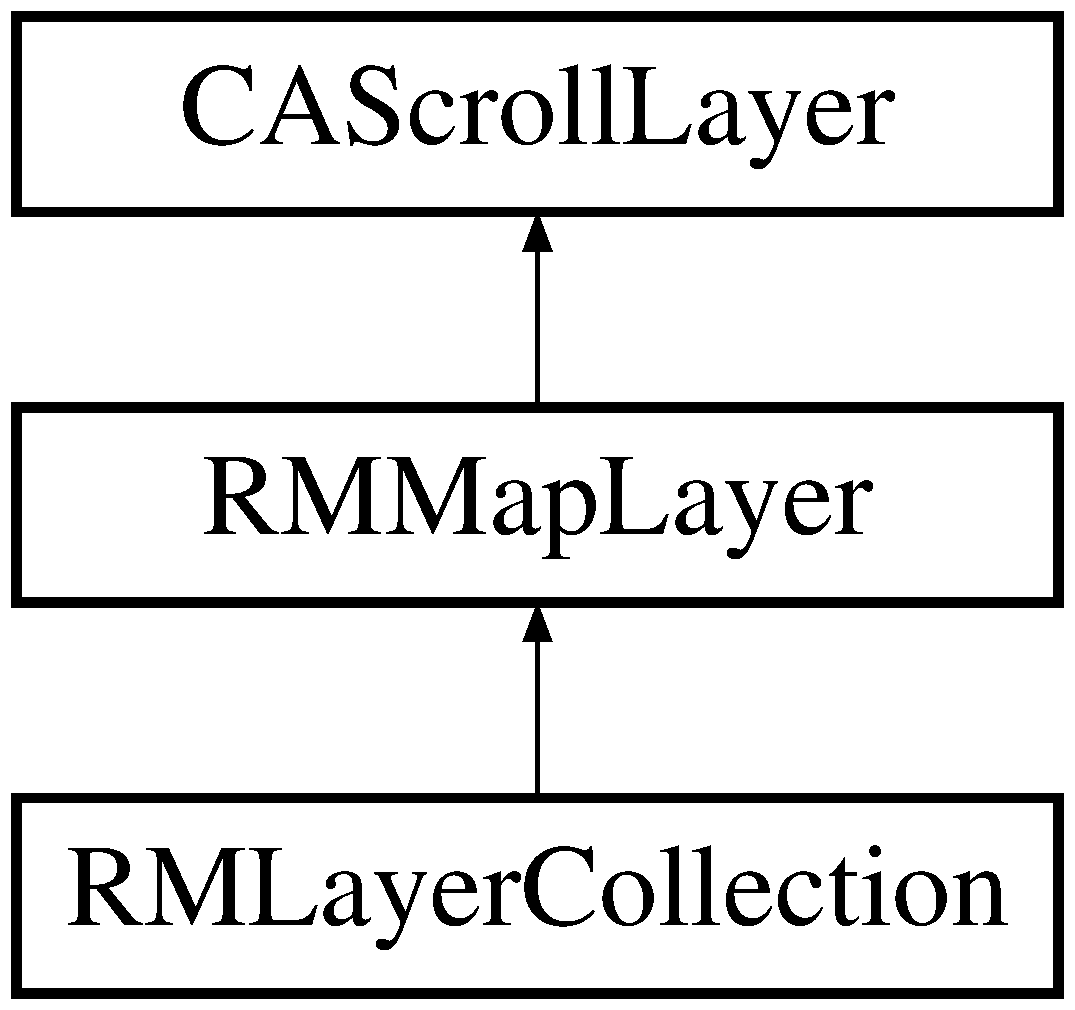
\includegraphics[height=3.000000cm]{interface_r_m_layer_collection}
\end{center}
\end{figure}
\subsection*{Instance Methods}
\begin{DoxyCompactItemize}
\item 
(void) -\/ \hyperlink{interface_r_m_layer_collection_a00588bd2c9488a450c8327b3de85bc88}{add\-Sublayer\-:}{\ttfamily  \mbox{[}implementation\mbox{]}}
\item 
(void) -\/ \hyperlink{interface_r_m_layer_collection_ab76d0a4f31f1617628edbdb6fe17b41e}{correct\-Position\-Of\-All\-Sublayers}
\begin{DoxyCompactList}\small\item\em (guess) recompute the screen coordinates for the sublayers (map markers, paths) \end{DoxyCompactList}\item 
(void) -\/ \hyperlink{interface_r_m_layer_collection_a9fdcb7e63266c915fbac013552c74da2}{correct\-Screen\-Position\-:}{\ttfamily  \mbox{[}implementation\mbox{]}}
\item 
(void) -\/ \hyperlink{interface_r_m_layer_collection_abc469c537574baa857ae981d193787ea}{dealloc}{\ttfamily  \mbox{[}implementation\mbox{]}}
\item 
(B\-O\-O\-L) -\/ \hyperlink{interface_r_m_layer_collection_a295705bf0ba820773f8d7a2ea002c670}{has\-Sub\-Layer\-:}
\item 
(id) -\/ \hyperlink{interface_r_m_layer_collection_a7691c224d9d64c8ed628187fb1b3b995}{init\-For\-Contents\-:}
\item 
(void) -\/ \hyperlink{interface_r_m_layer_collection_acc9f963b57d611df71a9604d208bb169}{insert\-Sublayer\-:above\-:}{\ttfamily  \mbox{[}implementation\mbox{]}}
\item 
(void) -\/ \hyperlink{interface_r_m_layer_collection_a2668330bd243651e532c232d932e0be1}{insert\-Sublayer\-:at\-Index\-:}{\ttfamily  \mbox{[}implementation\mbox{]}}
\item 
(void) -\/ \hyperlink{interface_r_m_layer_collection_a035dd534f0402568f3a8dcde1798710f}{insert\-Sublayer\-:below\-:}{\ttfamily  \mbox{[}implementation\mbox{]}}
\item 
(N\-S\-Integer) -\/ \hyperlink{interface_r_m_layer_collection_a302ebeb3ef7a162238e5f4060ca8f685}{layer\-Sort}{\ttfamily  \mbox{[}implementation\mbox{]}}
\item 
(void) -\/ \hyperlink{interface_r_m_layer_collection_aea4e071b3b6841f2892ff7dde0f737e6}{move\-By\-:}
\item 
(void) -\/ \hyperlink{interface_r_m_layer_collection_a34b34155a7d8dce54d35f8aca4346753}{move\-To\-Projected\-Point\-:}
\item 
(void) -\/ \hyperlink{interface_r_m_layer_collection_ac3857e4b024b2082e1934100aed5812c}{order\-Layers}
\begin{DoxyCompactList}\small\item\em Orders layers in the collection based on their position in the map, prioritizing instances/subclass instances of \hyperlink{interface_r_m_marker}{R\-M\-Marker} above other layers. This is called automatically in add\-Sublayer. \end{DoxyCompactList}\item 
(void) -\/ \hyperlink{interface_r_m_layer_collection_ab62813f526b09f2cff2ed323a2d4ade2}{remove\-Sublayer\-:}
\item 
(void) -\/ \hyperlink{interface_r_m_layer_collection_a46bd39dc6a8d9f35e76c87d681c0bb94}{remove\-Sublayers\-:}
\item 
(void) -\/ \hyperlink{interface_r_m_layer_collection_a903f17c4dfd80c96c8634eec45d60d51}{set\-Rotation\-Of\-All\-Sublayers\-:}
\item 
(void) -\/ \hyperlink{interface_r_m_layer_collection_a31a344ea9ba7e22761850589700b2fcf}{set\-Sublayers\-:}{\ttfamily  \mbox{[}implementation\mbox{]}}
\item 
(void) -\/ \hyperlink{interface_r_m_layer_collection_ade8dc9cb544571522ee47b35e124ac8e}{zoom\-By\-Factor\-:near\-:}
\end{DoxyCompactItemize}
\subsection*{Protected 属性}
\begin{DoxyCompactItemize}
\item 
\hyperlink{interface_r_m_map_contents}{R\-M\-Map\-Contents} $\ast$ \hyperlink{interface_r_m_layer_collection_ae66eb12ed40578ff23f20e54b28cfdb2}{map\-Contents}
\begin{DoxyCompactList}\small\item\em Backpointer to map; we need this reference so we can access the projections... \end{DoxyCompactList}\item 
C\-G\-Affine\-Transform \hyperlink{interface_r_m_layer_collection_a4586e34b2b33538246475b41e17d8534}{rotation\-Transform}
\item 
N\-S\-Mutable\-Array $\ast$ \hyperlink{interface_r_m_layer_collection_ae0741a32da2070098e364aac1c181256}{sublayers}
\begin{DoxyCompactList}\small\item\em The actual collection of all sublayers, including those offscreen. \end{DoxyCompactList}\end{DoxyCompactItemize}


\subsection{详细描述}
Appears to be some sort of interface between \hyperlink{interface_r_m_map_contents}{R\-M\-Map\-Contents} and markers. 

\begin{DoxyRefDesc}{Bug}
\item[\hyperlink{bug__bug000010}{Bug}]lots of arbitrary-\/appearing @synchronized blocks. Old mailing list traffic claims they're needed, but no one seems to know why. If the \#set ivar needs to be guarded, should be done by @synchronized(self) and not @synchronized(sublayers). Maybe the guarding is needed because of Core Animation thread interactions. \end{DoxyRefDesc}


\subsection{Method Documentation}
\hypertarget{interface_r_m_layer_collection_a00588bd2c9488a450c8327b3de85bc88}{\index{R\-M\-Layer\-Collection@{R\-M\-Layer\-Collection}!add\-Sublayer\-:@{add\-Sublayer\-:}}
\index{add\-Sublayer\-:@{add\-Sublayer\-:}!RMLayerCollection@{R\-M\-Layer\-Collection}}
\subsubsection[{add\-Sublayer\-:}]{\setlength{\rightskip}{0pt plus 5cm}-\/ (void) add\-Sublayer\-: 
\begin{DoxyParamCaption}
\item[{(C\-A\-Layer $\ast$)}]{layer}
\end{DoxyParamCaption}
\hspace{0.3cm}{\ttfamily [implementation]}}}\label{interface_r_m_layer_collection_a00588bd2c9488a450c8327b3de85bc88}


参考自 R\-M\-Marker\-Manager\-::add\-Marker\-:at\-Projected\-Point\-:.

\hypertarget{interface_r_m_layer_collection_ab76d0a4f31f1617628edbdb6fe17b41e}{\index{R\-M\-Layer\-Collection@{R\-M\-Layer\-Collection}!correct\-Position\-Of\-All\-Sublayers@{correct\-Position\-Of\-All\-Sublayers}}
\index{correct\-Position\-Of\-All\-Sublayers@{correct\-Position\-Of\-All\-Sublayers}!RMLayerCollection@{R\-M\-Layer\-Collection}}
\subsubsection[{correct\-Position\-Of\-All\-Sublayers}]{\setlength{\rightskip}{0pt plus 5cm}-\/ (void) correct\-Position\-Of\-All\-Sublayers 
\begin{DoxyParamCaption}
{}
\end{DoxyParamCaption}
}}\label{interface_r_m_layer_collection_ab76d0a4f31f1617628edbdb6fe17b41e}


(guess) recompute the screen coordinates for the sublayers (map markers, paths) 

\begin{DoxyRefDesc}{弃用}
\item[\hyperlink{deprecated__deprecated000001}{弃用}]name will change after 0.\-5 \end{DoxyRefDesc}


参考自 R\-M\-Map\-Contents\-::move\-By\-:, move\-To\-Projected\-Point\-:, R\-M\-Map\-Contents\-::set\-Center\-Projected\-Point\-:, R\-M\-Map\-Contents\-::set\-Frame\-:, R\-M\-Map\-Contents\-::set\-Meters\-Per\-Pixel\-:, R\-M\-Map\-Contents\-::zoom\-By\-Factor\-:near\-:, R\-M\-Map\-Contents\-::zoom\-By\-Factor\-:near\-:animated\-:with\-Callback\-: , 以及 R\-M\-Map\-Contents\-::zoom\-With\-R\-M\-Mercator\-Rect\-Bounds\-:.

\hypertarget{interface_r_m_layer_collection_a9fdcb7e63266c915fbac013552c74da2}{\index{R\-M\-Layer\-Collection@{R\-M\-Layer\-Collection}!correct\-Screen\-Position\-:@{correct\-Screen\-Position\-:}}
\index{correct\-Screen\-Position\-:@{correct\-Screen\-Position\-:}!RMLayerCollection@{R\-M\-Layer\-Collection}}
\subsubsection[{correct\-Screen\-Position\-:}]{\setlength{\rightskip}{0pt plus 5cm}-\/ (void) correct\-Screen\-Position\-: 
\begin{DoxyParamCaption}
\item[{(C\-A\-Layer $\ast$)}]{layer}
\end{DoxyParamCaption}
\hspace{0.3cm}{\ttfamily [implementation]}}}\label{interface_r_m_layer_collection_a9fdcb7e63266c915fbac013552c74da2}


参考自 add\-Sublayer\-:, correct\-Position\-Of\-All\-Sublayers, insert\-Sublayer\-:above\-:, insert\-Sublayer\-:at\-Index\-:, insert\-Sublayer\-:below\-: , 以及 set\-Sublayers\-:.

\hypertarget{interface_r_m_layer_collection_abc469c537574baa857ae981d193787ea}{\index{R\-M\-Layer\-Collection@{R\-M\-Layer\-Collection}!dealloc@{dealloc}}
\index{dealloc@{dealloc}!RMLayerCollection@{R\-M\-Layer\-Collection}}
\subsubsection[{dealloc}]{\setlength{\rightskip}{0pt plus 5cm}-\/ (void) dealloc 
\begin{DoxyParamCaption}
{}
\end{DoxyParamCaption}
\hspace{0.3cm}{\ttfamily [implementation]}}}\label{interface_r_m_layer_collection_abc469c537574baa857ae981d193787ea}
\hypertarget{interface_r_m_layer_collection_a295705bf0ba820773f8d7a2ea002c670}{\index{R\-M\-Layer\-Collection@{R\-M\-Layer\-Collection}!has\-Sub\-Layer\-:@{has\-Sub\-Layer\-:}}
\index{has\-Sub\-Layer\-:@{has\-Sub\-Layer\-:}!RMLayerCollection@{R\-M\-Layer\-Collection}}
\subsubsection[{has\-Sub\-Layer\-:}]{\setlength{\rightskip}{0pt plus 5cm}-\/ (B\-O\-O\-L) has\-Sub\-Layer\-: 
\begin{DoxyParamCaption}
\item[{(C\-A\-Layer $\ast$)}]{layer}
\end{DoxyParamCaption}
}}\label{interface_r_m_layer_collection_a295705bf0ba820773f8d7a2ea002c670}
\hypertarget{interface_r_m_layer_collection_a7691c224d9d64c8ed628187fb1b3b995}{\index{R\-M\-Layer\-Collection@{R\-M\-Layer\-Collection}!init\-For\-Contents\-:@{init\-For\-Contents\-:}}
\index{init\-For\-Contents\-:@{init\-For\-Contents\-:}!RMLayerCollection@{R\-M\-Layer\-Collection}}
\subsubsection[{init\-For\-Contents\-:}]{\setlength{\rightskip}{0pt plus 5cm}-\/ (id) init\-For\-Contents\-: 
\begin{DoxyParamCaption}
\item[{({\bf R\-M\-Map\-Contents} $\ast$)}]{contents}
\end{DoxyParamCaption}
}}\label{interface_r_m_layer_collection_a7691c224d9d64c8ed628187fb1b3b995}
\hypertarget{interface_r_m_layer_collection_acc9f963b57d611df71a9604d208bb169}{\index{R\-M\-Layer\-Collection@{R\-M\-Layer\-Collection}!insert\-Sublayer\-:above\-:@{insert\-Sublayer\-:above\-:}}
\index{insert\-Sublayer\-:above\-:@{insert\-Sublayer\-:above\-:}!RMLayerCollection@{R\-M\-Layer\-Collection}}
\subsubsection[{insert\-Sublayer\-:above\-:}]{\setlength{\rightskip}{0pt plus 5cm}-\/ (void) insert\-Sublayer\-: 
\begin{DoxyParamCaption}
\item[{(C\-A\-Layer $\ast$)}]{layer}
\item[{above:(C\-A\-Layer $\ast$)}]{sibling\-Layer}
\end{DoxyParamCaption}
\hspace{0.3cm}{\ttfamily [implementation]}}}\label{interface_r_m_layer_collection_acc9f963b57d611df71a9604d208bb169}
\hypertarget{interface_r_m_layer_collection_a2668330bd243651e532c232d932e0be1}{\index{R\-M\-Layer\-Collection@{R\-M\-Layer\-Collection}!insert\-Sublayer\-:at\-Index\-:@{insert\-Sublayer\-:at\-Index\-:}}
\index{insert\-Sublayer\-:at\-Index\-:@{insert\-Sublayer\-:at\-Index\-:}!RMLayerCollection@{R\-M\-Layer\-Collection}}
\subsubsection[{insert\-Sublayer\-:at\-Index\-:}]{\setlength{\rightskip}{0pt plus 5cm}-\/ (void) insert\-Sublayer\-: 
\begin{DoxyParamCaption}
\item[{(C\-A\-Layer $\ast$)}]{layer}
\item[{atIndex:(unsigned)}]{index}
\end{DoxyParamCaption}
\hspace{0.3cm}{\ttfamily [implementation]}}}\label{interface_r_m_layer_collection_a2668330bd243651e532c232d932e0be1}
\hypertarget{interface_r_m_layer_collection_a035dd534f0402568f3a8dcde1798710f}{\index{R\-M\-Layer\-Collection@{R\-M\-Layer\-Collection}!insert\-Sublayer\-:below\-:@{insert\-Sublayer\-:below\-:}}
\index{insert\-Sublayer\-:below\-:@{insert\-Sublayer\-:below\-:}!RMLayerCollection@{R\-M\-Layer\-Collection}}
\subsubsection[{insert\-Sublayer\-:below\-:}]{\setlength{\rightskip}{0pt plus 5cm}-\/ (void) insert\-Sublayer\-: 
\begin{DoxyParamCaption}
\item[{(C\-A\-Layer $\ast$)}]{layer}
\item[{below:(C\-A\-Layer $\ast$)}]{sibling\-Layer}
\end{DoxyParamCaption}
\hspace{0.3cm}{\ttfamily [implementation]}}}\label{interface_r_m_layer_collection_a035dd534f0402568f3a8dcde1798710f}
\hypertarget{interface_r_m_layer_collection_a302ebeb3ef7a162238e5f4060ca8f685}{\index{R\-M\-Layer\-Collection@{R\-M\-Layer\-Collection}!layer\-Sort@{layer\-Sort}}
\index{layer\-Sort@{layer\-Sort}!RMLayerCollection@{R\-M\-Layer\-Collection}}
\subsubsection[{layer\-Sort}]{\setlength{\rightskip}{0pt plus 5cm}-\/ (N\-S\-Integer) layer\-Sort 
\begin{DoxyParamCaption}
\item[{(id)}]{num1}
\item[{(id)}]{num2}
\item[{(void $\ast$)}]{context}
\end{DoxyParamCaption}
\hspace{0.3cm}{\ttfamily [implementation]}}}\label{interface_r_m_layer_collection_a302ebeb3ef7a162238e5f4060ca8f685}
\hypertarget{interface_r_m_layer_collection_aea4e071b3b6841f2892ff7dde0f737e6}{\index{R\-M\-Layer\-Collection@{R\-M\-Layer\-Collection}!move\-By\-:@{move\-By\-:}}
\index{move\-By\-:@{move\-By\-:}!RMLayerCollection@{R\-M\-Layer\-Collection}}
\subsubsection[{move\-By\-:}]{\setlength{\rightskip}{0pt plus 5cm}-\/ (void) move\-By\-: 
\begin{DoxyParamCaption}
\item[{(C\-G\-Size)}]{delta}
\end{DoxyParamCaption}
}}\label{interface_r_m_layer_collection_aea4e071b3b6841f2892ff7dde0f737e6}


重载 \hyperlink{interface_r_m_map_layer_ac960944a80c596eb918531cf63c54c11}{R\-M\-Map\-Layer} .



参考自 R\-M\-Map\-Contents\-::move\-By\-:.

\hypertarget{interface_r_m_layer_collection_a34b34155a7d8dce54d35f8aca4346753}{\index{R\-M\-Layer\-Collection@{R\-M\-Layer\-Collection}!move\-To\-Projected\-Point\-:@{move\-To\-Projected\-Point\-:}}
\index{move\-To\-Projected\-Point\-:@{move\-To\-Projected\-Point\-:}!RMLayerCollection@{R\-M\-Layer\-Collection}}
\subsubsection[{move\-To\-Projected\-Point\-:}]{\setlength{\rightskip}{0pt plus 5cm}-\/ (void) move\-To\-Projected\-Point\-: 
\begin{DoxyParamCaption}
\item[{({\bf R\-M\-Projected\-Point})}]{a\-Point}
\end{DoxyParamCaption}
}}\label{interface_r_m_layer_collection_a34b34155a7d8dce54d35f8aca4346753}
\begin{DoxyRefDesc}{Bug}
\item[\hyperlink{bug__bug000011}{Bug}]T\-O\-D\-O\-: Test this. Does it work? \end{DoxyRefDesc}
\hypertarget{interface_r_m_layer_collection_ac3857e4b024b2082e1934100aed5812c}{\index{R\-M\-Layer\-Collection@{R\-M\-Layer\-Collection}!order\-Layers@{order\-Layers}}
\index{order\-Layers@{order\-Layers}!RMLayerCollection@{R\-M\-Layer\-Collection}}
\subsubsection[{order\-Layers}]{\setlength{\rightskip}{0pt plus 5cm}-\/ (void) order\-Layers 
\begin{DoxyParamCaption}
{}
\end{DoxyParamCaption}
}}\label{interface_r_m_layer_collection_ac3857e4b024b2082e1934100aed5812c}


Orders layers in the collection based on their position in the map, prioritizing instances/subclass instances of \hyperlink{interface_r_m_marker}{R\-M\-Marker} above other layers. This is called automatically in add\-Sublayer. 

\hypertarget{interface_r_m_layer_collection_ab62813f526b09f2cff2ed323a2d4ade2}{\index{R\-M\-Layer\-Collection@{R\-M\-Layer\-Collection}!remove\-Sublayer\-:@{remove\-Sublayer\-:}}
\index{remove\-Sublayer\-:@{remove\-Sublayer\-:}!RMLayerCollection@{R\-M\-Layer\-Collection}}
\subsubsection[{remove\-Sublayer\-:}]{\setlength{\rightskip}{0pt plus 5cm}-\/ (void) remove\-Sublayer\-: 
\begin{DoxyParamCaption}
\item[{(C\-A\-Layer $\ast$)}]{layer}
\end{DoxyParamCaption}
}}\label{interface_r_m_layer_collection_ab62813f526b09f2cff2ed323a2d4ade2}


参考自 R\-M\-Marker\-Manager\-::remove\-Marker\-:.

\hypertarget{interface_r_m_layer_collection_a46bd39dc6a8d9f35e76c87d681c0bb94}{\index{R\-M\-Layer\-Collection@{R\-M\-Layer\-Collection}!remove\-Sublayers\-:@{remove\-Sublayers\-:}}
\index{remove\-Sublayers\-:@{remove\-Sublayers\-:}!RMLayerCollection@{R\-M\-Layer\-Collection}}
\subsubsection[{remove\-Sublayers\-:}]{\setlength{\rightskip}{0pt plus 5cm}-\/ (void) remove\-Sublayers\-: 
\begin{DoxyParamCaption}
\item[{(N\-S\-Array $\ast$)}]{layers}
\end{DoxyParamCaption}
}}\label{interface_r_m_layer_collection_a46bd39dc6a8d9f35e76c87d681c0bb94}


参考自 R\-M\-Marker\-Manager\-::remove\-Markers\-:.

\hypertarget{interface_r_m_layer_collection_a903f17c4dfd80c96c8634eec45d60d51}{\index{R\-M\-Layer\-Collection@{R\-M\-Layer\-Collection}!set\-Rotation\-Of\-All\-Sublayers\-:@{set\-Rotation\-Of\-All\-Sublayers\-:}}
\index{set\-Rotation\-Of\-All\-Sublayers\-:@{set\-Rotation\-Of\-All\-Sublayers\-:}!RMLayerCollection@{R\-M\-Layer\-Collection}}
\subsubsection[{set\-Rotation\-Of\-All\-Sublayers\-:}]{\setlength{\rightskip}{0pt plus 5cm}-\/ (void) set\-Rotation\-Of\-All\-Sublayers\-: 
\begin{DoxyParamCaption}
\item[{(float)}]{angle}
\end{DoxyParamCaption}
}}\label{interface_r_m_layer_collection_a903f17c4dfd80c96c8634eec45d60d51}


参考自 R\-M\-Map\-Contents\-::set\-Rotation\-:.

\hypertarget{interface_r_m_layer_collection_a31a344ea9ba7e22761850589700b2fcf}{\index{R\-M\-Layer\-Collection@{R\-M\-Layer\-Collection}!set\-Sublayers\-:@{set\-Sublayers\-:}}
\index{set\-Sublayers\-:@{set\-Sublayers\-:}!RMLayerCollection@{R\-M\-Layer\-Collection}}
\subsubsection[{set\-Sublayers\-:}]{\setlength{\rightskip}{0pt plus 5cm}-\/ (void) set\-Sublayers\-: 
\begin{DoxyParamCaption}
\item[{(N\-S\-Array$\ast$)}]{array}
\end{DoxyParamCaption}
\hspace{0.3cm}{\ttfamily [implementation]}}}\label{interface_r_m_layer_collection_a31a344ea9ba7e22761850589700b2fcf}


参考自 R\-M\-Marker\-Manager\-::remove\-Markers.

\hypertarget{interface_r_m_layer_collection_ade8dc9cb544571522ee47b35e124ac8e}{\index{R\-M\-Layer\-Collection@{R\-M\-Layer\-Collection}!zoom\-By\-Factor\-:near\-:@{zoom\-By\-Factor\-:near\-:}}
\index{zoom\-By\-Factor\-:near\-:@{zoom\-By\-Factor\-:near\-:}!RMLayerCollection@{R\-M\-Layer\-Collection}}
\subsubsection[{zoom\-By\-Factor\-:near\-:}]{\setlength{\rightskip}{0pt plus 5cm}-\/ (void) zoom\-By\-Factor\-: 
\begin{DoxyParamCaption}
\item[{(float)}]{zoom\-Factor}
\item[{near:(C\-G\-Point)}]{center}
\end{DoxyParamCaption}
}}\label{interface_r_m_layer_collection_ade8dc9cb544571522ee47b35e124ac8e}


重载 \hyperlink{interface_r_m_map_layer_ae0e1f8c364aaca4ac39766fe14bbba07}{R\-M\-Map\-Layer} .



参考自 R\-M\-Map\-Contents\-::set\-Meters\-Per\-Pixel\-:, R\-M\-Map\-Contents\-::zoom\-By\-Factor\-:near\-: , 以及 R\-M\-Map\-Contents\-::zoom\-By\-Factor\-:near\-:animated\-:with\-Callback\-:.



\subsection{类成员变量说明}
\hypertarget{interface_r_m_layer_collection_ae66eb12ed40578ff23f20e54b28cfdb2}{\index{R\-M\-Layer\-Collection@{R\-M\-Layer\-Collection}!map\-Contents@{map\-Contents}}
\index{map\-Contents@{map\-Contents}!RMLayerCollection@{R\-M\-Layer\-Collection}}
\subsubsection[{map\-Contents}]{\setlength{\rightskip}{0pt plus 5cm}-\/ ({\bf R\-M\-Map\-Contents}$\ast$) map\-Contents\hspace{0.3cm}{\ttfamily [protected]}}}\label{interface_r_m_layer_collection_ae66eb12ed40578ff23f20e54b28cfdb2}


Backpointer to map; we need this reference so we can access the projections... 



参考自 correct\-Screen\-Position\-:, dealloc , 以及 init\-For\-Contents\-:.

\hypertarget{interface_r_m_layer_collection_a4586e34b2b33538246475b41e17d8534}{\index{R\-M\-Layer\-Collection@{R\-M\-Layer\-Collection}!rotation\-Transform@{rotation\-Transform}}
\index{rotation\-Transform@{rotation\-Transform}!RMLayerCollection@{R\-M\-Layer\-Collection}}
\subsubsection[{rotation\-Transform}]{\setlength{\rightskip}{0pt plus 5cm}-\/ (C\-G\-Affine\-Transform) rotation\-Transform\hspace{0.3cm}{\ttfamily [protected]}}}\label{interface_r_m_layer_collection_a4586e34b2b33538246475b41e17d8534}


参考自 init\-For\-Contents\-: , 以及 set\-Rotation\-Of\-All\-Sublayers\-:.

\hypertarget{interface_r_m_layer_collection_ae0741a32da2070098e364aac1c181256}{\index{R\-M\-Layer\-Collection@{R\-M\-Layer\-Collection}!sublayers@{sublayers}}
\index{sublayers@{sublayers}!RMLayerCollection@{R\-M\-Layer\-Collection}}
\subsubsection[{sublayers}]{\setlength{\rightskip}{0pt plus 5cm}-\/ (N\-S\-Mutable\-Array$\ast$) sublayers\hspace{0.3cm}{\ttfamily [protected]}}}\label{interface_r_m_layer_collection_ae0741a32da2070098e364aac1c181256}


The actual collection of all sublayers, including those offscreen. 

It is ordered back to front. 

参考自 add\-Sublayer\-:, correct\-Position\-Of\-All\-Sublayers, dealloc, has\-Sub\-Layer\-:, init\-For\-Contents\-:, insert\-Sublayer\-:above\-:, insert\-Sublayer\-:at\-Index\-:, insert\-Sublayer\-:below\-:, R\-M\-Marker\-Manager\-::markers, move\-By\-:, remove\-Sublayer\-:, remove\-Sublayers\-:, set\-Rotation\-Of\-All\-Sublayers\-:, set\-Sublayers\-: , 以及 zoom\-By\-Factor\-:near\-:.



该类的文档由以下文件生成\-:\begin{DoxyCompactItemize}
\item 
Map/\hyperlink{_r_m_layer_collection_8h}{R\-M\-Layer\-Collection.\-h}\item 
Map/\hyperlink{_r_m_layer_collection_8m}{R\-M\-Layer\-Collection.\-m}\end{DoxyCompactItemize}

\hypertarget{interface_r_m_map_contents}{\section{R\-M\-Map\-Contents类 参考}
\label{interface_r_m_map_contents}\index{R\-M\-Map\-Contents@{R\-M\-Map\-Contents}}
}


The cartographic and data components of a map.  




{\ttfamily \#import $<$R\-M\-Map\-Contents.\-h$>$}

类 R\-M\-Map\-Contents 继承关系图\-:\begin{figure}[H]
\begin{center}
\leavevmode
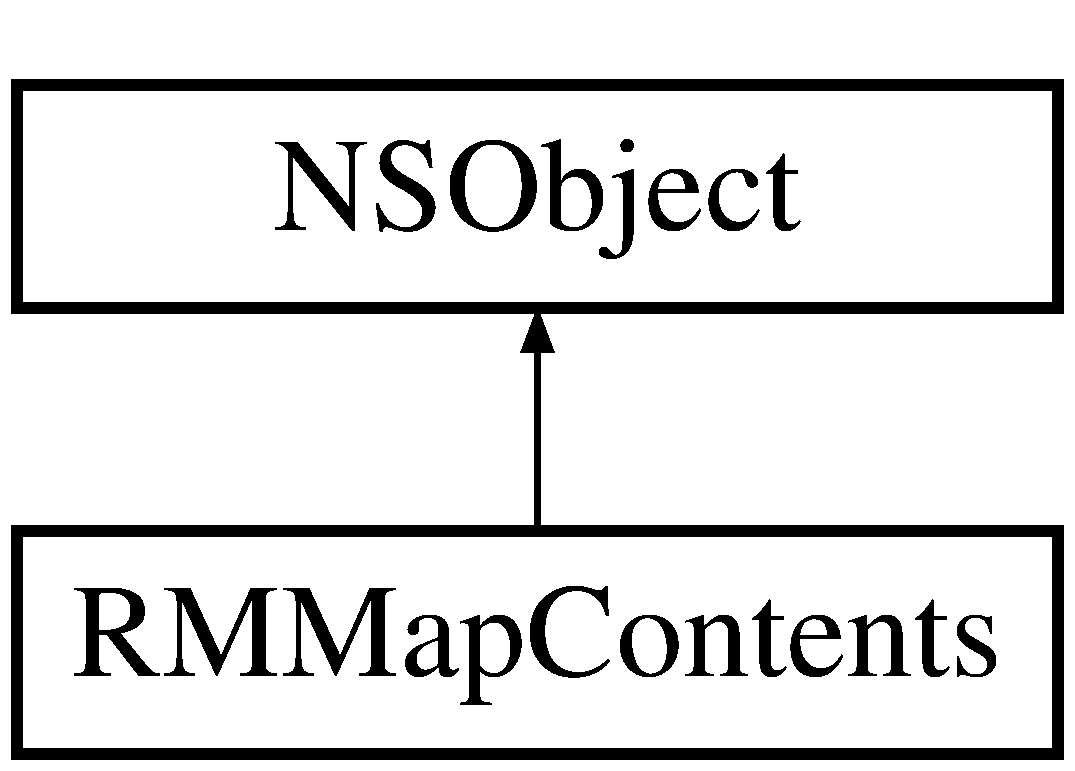
\includegraphics[height=2.000000cm]{interface_r_m_map_contents}
\end{center}
\end{figure}
\subsection*{Instance Methods}
\begin{DoxyCompactItemize}
\item 
(void) -\/ \hyperlink{interface_r_m_map_contents_ad5e13a19a28049128f6a9eb36415eb71}{adjust\-Map\-Placement\-With\-Scale\-:}
\begin{DoxyCompactList}\small\item\em This currently is not called because it does not handle the case when the map is continous or not continous. \end{DoxyCompactList}\item 
(float) -\/ \hyperlink{interface_r_m_map_contents_a08e2f802b9fa6d0cfe3478725684545e}{adjust\-Zoom\-For\-Bounding\-Mask\-:}
\item 
(void) -\/ \hyperlink{interface_r_m_map_contents_a1d3d6d5bd375efa2b6926494150a2f4f}{animated\-Zoom\-Step\-:}{\ttfamily  \mbox{[}implementation\mbox{]}}
\item 
(void) -\/ \hyperlink{interface_r_m_map_contents_a528c6e073c6c8308771f9d71f16a9bf4}{dealloc}{\ttfamily  \mbox{[}implementation\mbox{]}}
\item 
(void) -\/ \hyperlink{interface_r_m_map_contents_ad715d6e1088cf3994b26f7ab6cacf391}{did\-Receive\-Memory\-Warning}
\item 
(void) -\/ \hyperlink{interface_r_m_map_contents_a5bcdc830d59d045abc4fdf2c57fef8cb}{draw\-Rect\-:}
\item 
(void) -\/ \hyperlink{interface_r_m_map_contents_a5e5cb1f8dbb78ee775e5ccc9703ceb3f}{handle\-Memory\-Warning\-Notification\-:}
\item 
(id) -\/ \hyperlink{interface_r_m_map_contents_a3f56aed0e38083d5fc613887f626210b}{init\-For\-View\-:}
\begin{DoxyCompactList}\small\item\em deprecated at any moment after release 0.\-5 \end{DoxyCompactList}\item 
(id) -\/ \hyperlink{interface_r_m_map_contents_a5ac0e7aeea1edca790b2466a62714786}{init\-For\-View\-:\-With\-Location\-:}
\begin{DoxyCompactList}\small\item\em deprecated at any moment after release 0.\-5 \end{DoxyCompactList}\item 
(id) -\/ \hyperlink{interface_r_m_map_contents_ac88a327e2895d4d95c9fc829ab99294d}{init\-For\-View\-:\-With\-Tile\-Source\-:\-With\-Renderer\-:\-Looking\-At\-:}
\begin{DoxyCompactList}\small\item\em deprecated at any moment after release 0.\-5 \end{DoxyCompactList}\item 
(id) -\/ \hyperlink{interface_r_m_map_contents_ade383b6491bd769a6bb17f5d5b0c107e}{init\-With\-View\-:}
\item 
(id) -\/ \hyperlink{interface_r_m_map_contents_ade6f726a40417c75537812d02a0f9c6c}{init\-With\-View\-:screen\-Scale\-:}
\item 
(id) -\/ \hyperlink{interface_r_m_map_contents_a9c237b4599ba3e90db2ab34f40aab601}{init\-With\-View\-:tilesource\-:}
\item 
(id) -\/ \hyperlink{interface_r_m_map_contents_a6196963182efcdf037319e622f4ca2d8}{init\-With\-View\-:tilesource\-:center\-Lat\-Lon\-:zoom\-Level\-:max\-Zoom\-Level\-:min\-Zoom\-Level\-:background\-Image\-:screen\-Scale\-:}
\begin{DoxyCompactList}\small\item\em designated initializer \end{DoxyCompactList}\item 
(id) -\/ \hyperlink{interface_r_m_map_contents_ade69d06fda9b105ca86b023926e0bb21}{init\-With\-View\-:tilesource\-:screen\-Scale\-:}
\item 
(\hyperlink{struct_r_m_spherical_trapezium}{R\-M\-Spherical\-Trapezium}) -\/ \hyperlink{interface_r_m_map_contents_a9886560e7143a571c5be1260686dd7b6}{latitude\-Longitude\-Bounding\-Box\-For\-:}
\begin{DoxyCompactList}\small\item\em returns the smallest bounding box containing a rectangular region of the screen \end{DoxyCompactList}\item 
(\hyperlink{struct_r_m_spherical_trapezium}{R\-M\-Spherical\-Trapezium}) -\/ \hyperlink{interface_r_m_map_contents_a2f036b07434552724b6ad3d56f6e6ed6}{latitude\-Longitude\-Bounding\-Box\-For\-Screen}
\begin{DoxyCompactList}\small\item\em returns the smallest bounding box containing the entire screen \end{DoxyCompactList}\item 
(C\-G\-Point) -\/ \hyperlink{interface_r_m_map_contents_a80f4f3e3dcf962c4d1110248e5f83ff6}{lat\-Long\-To\-Pixel\-:}
\item 
(C\-G\-Point) -\/ \hyperlink{interface_r_m_map_contents_a6c7d5693a725d88769b5377d60cab941}{lat\-Long\-To\-Pixel\-:with\-Meters\-Per\-Pixel\-:}
\item 
(\hyperlink{struct_r_m_tile_point}{R\-M\-Tile\-Point}) -\/ \hyperlink{interface_r_m_map_contents_af5abbc64cb02512eb4378fce3794f0e1}{lat\-Long\-To\-Tile\-Point\-:with\-Meters\-Per\-Pixel\-:}
\item 
(void) -\/ \hyperlink{interface_r_m_map_contents_af3baee3fc58a0b88ecd7a9ec8c7cbe88}{move\-By\-:}
\item 
(void) -\/ \hyperlink{interface_r_m_map_contents_a6964b2e4a12c17c954d32dc8e8fe739e}{move\-To\-Lat\-Long\-:}
\item 
(void) -\/ \hyperlink{interface_r_m_map_contents_a6bf308257eae65ff4037a4e5654f8c46}{move\-To\-Projected\-Point\-:}
\begin{DoxyCompactList}\small\item\em Use set\-Center\-Projected\-Point\-: instead. \end{DoxyCompactList}\item 
(float) -\/ \hyperlink{interface_r_m_map_contents_a62632c7f86a830a06afbc6f47f8b3fdf}{next\-Native\-Zoom\-Factor}
\item 
(C\-L\-Location\-Coordinate2\-D) -\/ \hyperlink{interface_r_m_map_contents_ad7f1b803be32266a8a0bc5de03fd4e0e}{pixel\-To\-Lat\-Long\-:}
\item 
(C\-L\-Location\-Coordinate2\-D) -\/ \hyperlink{interface_r_m_map_contents_a5fe69ea6a21dac1fdc4c6d136d1a1504}{pixel\-To\-Lat\-Long\-:with\-Meters\-Per\-Pixel\-:}
\item 
(float) -\/ \hyperlink{interface_r_m_map_contents_aef141216ceb8e4c044e83e6ba8a9b7b1}{prev\-Native\-Zoom\-Factor}
\item 
(void) -\/ \hyperlink{interface_r_m_map_contents_a2d6c92fc5d07149961988b7ed062021c}{print\-Debugging\-Information}{\ttfamily  \mbox{[}implementation\mbox{]}}
\item 
(void) -\/ \hyperlink{interface_r_m_map_contents_a05e9ebea304077388c28e5306459ad96}{remove\-All\-Cached\-Images}
\begin{DoxyCompactList}\small\item\em Clear all images from the \hyperlink{interface_r_m_map_contents_afdc2f45aee8bcc5633182450fdea0cfc}{tile\-Source}'s caching system. \end{DoxyCompactList}\item 
(void) -\/ \hyperlink{interface_r_m_map_contents_ac5fb96bc69e7ac42b6a43aff804dc72c}{set\-Background\-:}{\ttfamily  \mbox{[}implementation\mbox{]}}
\item 
(void) -\/ \hyperlink{interface_r_m_map_contents_af156345c10a07045bbedec55efe6247e}{set\-Center\-Projected\-Point\-:}{\ttfamily  \mbox{[}implementation\mbox{]}}
\item 
(void) -\/ \hyperlink{interface_r_m_map_contents_a8bb51badbffed49e25be29edafb10a95}{set\-Frame\-:}
\item 
(void) -\/ \hyperlink{interface_r_m_map_contents_a7787b10ca141e7fdaf6e99312d4f5504}{set\-Map\-Center\-:}{\ttfamily  \mbox{[}implementation\mbox{]}}
\item 
(void) -\/ \hyperlink{interface_r_m_map_contents_a2668247ea9686a5d84aff8db823b1cf6}{set\-Max\-Zoom\-:}{\ttfamily  \mbox{[}implementation\mbox{]}}
\item 
(void) -\/ \hyperlink{interface_r_m_map_contents_a56e7ec20e0ef55c9bdceb73dee05a1aa}{set\-Meters\-Per\-Pixel\-:}{\ttfamily  \mbox{[}implementation\mbox{]}}
\item 
(void) -\/ \hyperlink{interface_r_m_map_contents_a5c2eda436f8e54cbed7263e419046cd1}{set\-Min\-Zoom\-:}{\ttfamily  \mbox{[}implementation\mbox{]}}
\item 
(void) -\/ \hyperlink{interface_r_m_map_contents_ad20f344bc5c5361cc12a08bb1221f766}{set\-Overlay\-:}{\ttfamily  \mbox{[}implementation\mbox{]}}
\item 
(void) -\/ \hyperlink{interface_r_m_map_contents_ad94e75ab1195d755f8f52caba2fc554f}{set\-Projected\-Bounds\-:}{\ttfamily  \mbox{[}implementation\mbox{]}}
\item 
(void) -\/ \hyperlink{interface_r_m_map_contents_ab3dc71cf707383671723a0629bbf6587}{set\-Renderer\-:}{\ttfamily  \mbox{[}implementation\mbox{]}}
\item 
(void) -\/ \hyperlink{interface_r_m_map_contents_a8c9d36abec740f7a9c7047fa1f47daa5}{set\-Rotation\-:}
\item 
(void) -\/ \hyperlink{interface_r_m_map_contents_a9de0ef8146a2ec46e7bca53bbd763bec}{set\-Scaled\-Meters\-Per\-Pixel\-:}{\ttfamily  \mbox{[}implementation\mbox{]}}
\item 
(void) -\/ \hyperlink{interface_r_m_map_contents_ae33000c5144c046f9d4da1d20b80004c}{set\-Tile\-Depth\-:}{\ttfamily  \mbox{[}implementation\mbox{]}}
\item 
(void) -\/ \hyperlink{interface_r_m_map_contents_a69a041eb8065efe8f31ce40ad9894f1c}{set\-Tile\-Source\-:}{\ttfamily  \mbox{[}implementation\mbox{]}}
\item 
(void) -\/ \hyperlink{interface_r_m_map_contents_afbdfe65940239191436f23b14942bb2e}{set\-Tiles\-Update\-Delegate\-:}{\ttfamily  \mbox{[}implementation\mbox{]}}
\item 
(void) -\/ \hyperlink{interface_r_m_map_contents_a06f80b8cd231adf996ed5c363afa34f8}{set\-Zoom\-:}{\ttfamily  \mbox{[}implementation\mbox{]}}
\begin{DoxyCompactList}\small\item\em if \hyperlink{interface_r_m_map_contents_a199c766d9970b90672f8884856c7cd4e}{zoom} is outside of range \hyperlink{interface_r_m_map_contents_ab434ff9dc95d209ad2d53cf8d0f1703b}{min\-Zoom} to \hyperlink{interface_r_m_map_contents_afa0fef34433cbc987d0346dccbd151a1}{max\-Zoom}, zoom level is clamped to that range. \end{DoxyCompactList}\item 
(B\-O\-O\-L) -\/ \hyperlink{interface_r_m_map_contents_a0d412fc8ab80b4ef35c2dabf3a0f1c12}{should\-Zoom\-To\-Target\-Zoom\-:with\-Zoom\-Factor\-:}{\ttfamily  \mbox{[}implementation\mbox{]}}
\item 
(void) -\/ \hyperlink{interface_r_m_map_contents_a78107eb32326f58654bd9bcfe04c8289}{tiles\-Updated\-Region\-:}
\item 
(void) -\/ \hyperlink{interface_r_m_map_contents_ac84735b91375863f930ce3465411a85f}{zoom\-By\-Factor\-:near\-:}
\item 
(void) -\/ \hyperlink{interface_r_m_map_contents_a50036c154b99004fef1068a4972bd941}{zoom\-By\-Factor\-:near\-:animated\-:}
\item 
(void) -\/ \hyperlink{interface_r_m_map_contents_a625f32a99c58256644eeef69d40e13a9}{zoom\-By\-Factor\-:near\-:animated\-:with\-Callback\-:}
\item 
(void) -\/ \hyperlink{interface_r_m_map_contents_a8f2944077cd2d27c01463fa4881d3152}{zoom\-In\-To\-Next\-Native\-Zoom\-At\-:}
\item 
(void) -\/ \hyperlink{interface_r_m_map_contents_a6c5bafdae9d97c075ef057f78f3c38e6}{zoom\-In\-To\-Next\-Native\-Zoom\-At\-:animated\-:}
\item 
(void) -\/ \hyperlink{interface_r_m_map_contents_a4d5461e344f8d9f3567064f5749baf1f}{zoom\-Out\-To\-Next\-Native\-Zoom\-At\-:}
\item 
(void) -\/ \hyperlink{interface_r_m_map_contents_af50e2b740deeaf047fd114888c14c042}{zoom\-Out\-To\-Next\-Native\-Zoom\-At\-:animated\-:}
\item 
(void) -\/ \hyperlink{interface_r_m_map_contents_a16518ad8c17a80bc90fbb396f4d9d16b}{zoom\-With\-Lat\-Lng\-Bounds\-North\-East\-:\-South\-West\-:}
\item 
(void) -\/ \hyperlink{interface_r_m_map_contents_a527d09084d834ec9cc4738ba6ebba397}{zoom\-With\-R\-M\-Mercator\-Rect\-Bounds\-:}
\end{DoxyCompactItemize}
\subsection*{Class Methods}
\begin{DoxyCompactItemize}
\item 
(B\-O\-O\-L) + \hyperlink{interface_r_m_map_contents_a65e78425d0827ed394433fb9aca11a62}{perform\-Expensive\-Operations}
\item 
(void) + \hyperlink{interface_r_m_map_contents_aa00c82eeeb84859798f03e09226a8100}{set\-Perform\-Expensive\-Operations\-:}
\end{DoxyCompactItemize}
\subsection*{属性}
\begin{DoxyCompactItemize}
\item 
\hyperlink{interface_r_m_map_layer}{R\-M\-Map\-Layer} $\ast$ \hyperlink{interface_r_m_map_contents_a220a37d482a030e392788dee48ffc108}{background}
\begin{DoxyCompactList}\small\item\em subview for the image displayed while tiles are loading. Set its contents by providing your own \char`\"{}loading.\-png\char`\"{}. \end{DoxyCompactList}\item 
N\-S\-U\-Integer \hyperlink{interface_r_m_map_contents_a1ab8589d1d1fc05208eaffefcff9edaf}{bounding\-Mask}
\item 
\hyperlink{struct_r_m_projected_point}{R\-M\-Projected\-Point} \hyperlink{interface_r_m_map_contents_ae370cf3845309794b89e5b11290b520e}{center\-Projected\-Point}
\item 
B\-O\-O\-L \hyperlink{interface_r_m_map_contents_af81fdb306fe5675cc9ebc223379c773a}{fully\-Loaded}
\item 
\hyperlink{interface_r_m_tile_image_set}{R\-M\-Tile\-Image\-Set} $\ast$ \hyperlink{interface_r_m_map_contents_a4da52b65a26cd078dfa90c2d348c58c0}{images\-On\-Screen}
\item 
C\-A\-Layer $\ast$ \hyperlink{interface_r_m_map_contents_afba5a8749837d703d4c551c12e134c54}{layer}
\begin{DoxyCompactList}\small\item\em This is the underlying U\-I\-View's layer. \end{DoxyCompactList}\item 
C\-L\-Location\-Coordinate2\-D \hyperlink{interface_r_m_map_contents_a66dc32c1210bd62ef66dd729aebcf55c}{map\-Center}
\item 
\hyperlink{interface_r_m_marker_manager}{R\-M\-Marker\-Manager} $\ast$ \hyperlink{interface_r_m_map_contents_a2e28d0b3c7f2670181edb8b87ab0324f}{marker\-Manager}
\item 
float \hyperlink{interface_r_m_map_contents_afa0fef34433cbc987d0346dccbd151a1}{max\-Zoom}
\begin{DoxyCompactList}\small\item\em maximum zoom number allowed for the view. \hyperlink{interface_r_m_map_contents_ab434ff9dc95d209ad2d53cf8d0f1703b}{min\-Zoom} and \hyperlink{interface_r_m_map_contents_afa0fef34433cbc987d0346dccbd151a1}{max\-Zoom} must be within the limits of \hyperlink{interface_r_m_map_contents_afdc2f45aee8bcc5633182450fdea0cfc}{tile\-Source} but can be stricter; they are clamped to tilesource limits if needed. \end{DoxyCompactList}\item 
\hyperlink{interface_r_m_mercator_to_screen_projection}{R\-M\-Mercator\-To\-Screen\-Projection} $\ast$ \hyperlink{interface_r_m_map_contents_ac90bc80b3d40b418ff2fa21dc35cf6ca}{mercator\-To\-Screen\-Projection}
\begin{DoxyCompactList}\small\item\em (guess) converts from projected meters to screen pixel coordinates \end{DoxyCompactList}\item 
id$<$ \hyperlink{protocol_r_m_mercator_to_tile_projection-p}{R\-M\-Mercator\-To\-Tile\-Projection} $>$ \hyperlink{interface_r_m_map_contents_a3e7903c036affb0241bc13e128574073}{mercator\-To\-Tile\-Projection}
\item 
float \hyperlink{interface_r_m_map_contents_a23204276fe6140d07d3671e9b90157dc}{meters\-Per\-Pixel}
\item 
float \hyperlink{interface_r_m_map_contents_ab434ff9dc95d209ad2d53cf8d0f1703b}{min\-Zoom}
\begin{DoxyCompactList}\small\item\em minimum zoom number allowed for the view. \hyperlink{interface_r_m_map_contents_ab434ff9dc95d209ad2d53cf8d0f1703b}{min\-Zoom} and \hyperlink{interface_r_m_map_contents_afa0fef34433cbc987d0346dccbd151a1}{max\-Zoom} must be within the limits of \hyperlink{interface_r_m_map_contents_afdc2f45aee8bcc5633182450fdea0cfc}{tile\-Source} but can be stricter; they are clamped to tilesource limits if needed. \end{DoxyCompactList}\item 
\hyperlink{interface_r_m_layer_collection}{R\-M\-Layer\-Collection} $\ast$ \hyperlink{interface_r_m_map_contents_ae5474cf3d2df7f969aec0944ac02134c}{overlay}
\begin{DoxyCompactList}\small\item\em subview for markers and paths \end{DoxyCompactList}\item 
\hyperlink{struct_r_m_projected_rect}{R\-M\-Projected\-Rect} \hyperlink{interface_r_m_map_contents_a46afa80adb2b126e05dfaf6501f17eea}{projected\-Bounds}
\item 
\hyperlink{interface_r_m_projection}{R\-M\-Projection} $\ast$ \hyperlink{interface_r_m_map_contents_ac83cbe1542e19defe75afc557007e282}{projection}
\begin{DoxyCompactList}\small\item\em (guess) the projection object to convert from latitude/longitude to meters. \end{DoxyCompactList}\item 
\hyperlink{interface_r_m_map_renderer}{R\-M\-Map\-Renderer} $\ast$ \hyperlink{interface_r_m_map_contents_a5054d0d02002aa0757df91c9567d0cd9}{renderer}
\item 
double \hyperlink{interface_r_m_map_contents_a5f23576d9f94b8528a3886af2013144d}{scale\-Denominator}
\begin{DoxyCompactList}\small\item\em The denominator in a cartographic scale like 1/24000, 1/50000, 1/2000000. \end{DoxyCompactList}\item 
float \hyperlink{interface_r_m_map_contents_a1ad726ecd59ef33b559d35c8d1cef95e}{scaled\-Meters\-Per\-Pixel}
\item 
C\-G\-Rect \hyperlink{interface_r_m_map_contents_a658f2c0b02e7dded8f625329c658f925}{screen\-Bounds}
\item 
float \hyperlink{interface_r_m_map_contents_aeae93353d6604c3304d945da9490d809}{screen\-Scale}
\item 
\hyperlink{struct_r_m_tile_rect}{R\-M\-Tile\-Rect} \hyperlink{interface_r_m_map_contents_a385e41b3717e62ef1d343b73144c1ef4}{tile\-Bounds}
\item 
short \hyperlink{interface_r_m_map_contents_ad55a0b34afd6bd4b228f8ae3555f7d98}{tile\-Depth}
\item 
\hyperlink{interface_r_m_tile_loader}{R\-M\-Tile\-Loader} $\ast$ \hyperlink{interface_r_m_map_contents_ad7c6bc753e0b9a1cbaa5e9dcb4a5e853}{tile\-Loader}
\item 
id$<$ \hyperlink{protocol_r_m_tile_source-p}{R\-M\-Tile\-Source} $>$ \hyperlink{interface_r_m_map_contents_afdc2f45aee8bcc5633182450fdea0cfc}{tile\-Source}
\begin{DoxyCompactList}\small\item\em controls what images are used. Can be changed while the view is visible, but see \href{http://code.google.com/p/route-me/issues/detail?id=12}{\tt http\-://code.\-google.\-com/p/route-\/me/issues/detail?id=12} \end{DoxyCompactList}\item 
id$<$ \hyperlink{protocol_r_m_tiles_update_delegate-p}{R\-M\-Tiles\-Update\-Delegate} $>$ \hyperlink{interface_r_m_map_contents_a37fd1037d5c01ab7543a46056039ec77}{tiles\-Update\-Delegate}
\item 
float \hyperlink{interface_r_m_map_contents_a199c766d9970b90672f8884856c7cd4e}{zoom}
\begin{DoxyCompactList}\small\item\em zoom level is clamped to range (min\-Zoom, max\-Zoom) \end{DoxyCompactList}\end{DoxyCompactItemize}


\subsection{详细描述}
The cartographic and data components of a map. 

Do not retain.

There is exactly one \hyperlink{interface_r_m_map_contents}{R\-M\-Map\-Contents} instance for each \hyperlink{interface_r_m_map_view}{R\-M\-Map\-View} instance.

\begin{DoxyWarning}{警告}
Do not retain an \hyperlink{interface_r_m_map_contents}{R\-M\-Map\-Contents} instance. Instead, ask the \hyperlink{interface_r_m_map_view}{R\-M\-Map\-View} for its contents when you need it. It is an error for an \hyperlink{interface_r_m_map_contents}{R\-M\-Map\-Contents} instance to exist without a view, and if you retain the \hyperlink{interface_r_m_map_contents}{R\-M\-Map\-Contents}, it can't go away when the \hyperlink{interface_r_m_map_view}{R\-M\-Map\-View} is released.
\end{DoxyWarning}
At some point, it's likely that \hyperlink{interface_r_m_map_contents}{R\-M\-Map\-Contents} and \hyperlink{interface_r_m_map_view}{R\-M\-Map\-View} will be merged into one class. 

\subsection{Method Documentation}
\hypertarget{interface_r_m_map_contents_ad5e13a19a28049128f6a9eb36415eb71}{\index{R\-M\-Map\-Contents@{R\-M\-Map\-Contents}!adjust\-Map\-Placement\-With\-Scale\-:@{adjust\-Map\-Placement\-With\-Scale\-:}}
\index{adjust\-Map\-Placement\-With\-Scale\-:@{adjust\-Map\-Placement\-With\-Scale\-:}!RMMapContents@{R\-M\-Map\-Contents}}
\subsubsection[{adjust\-Map\-Placement\-With\-Scale\-:}]{\setlength{\rightskip}{0pt plus 5cm}-\/ (void) adjust\-Map\-Placement\-With\-Scale\-: 
\begin{DoxyParamCaption}
\item[{(float)}]{a\-Scale}
\end{DoxyParamCaption}
}}\label{interface_r_m_map_contents_ad5e13a19a28049128f6a9eb36415eb71}


This currently is not called because it does not handle the case when the map is continous or not continous. 

At a certain scale you can continuously move to the west or east until you get to a certain scale level that simply shows the entire world. \hypertarget{interface_r_m_map_contents_a08e2f802b9fa6d0cfe3478725684545e}{\index{R\-M\-Map\-Contents@{R\-M\-Map\-Contents}!adjust\-Zoom\-For\-Bounding\-Mask\-:@{adjust\-Zoom\-For\-Bounding\-Mask\-:}}
\index{adjust\-Zoom\-For\-Bounding\-Mask\-:@{adjust\-Zoom\-For\-Bounding\-Mask\-:}!RMMapContents@{R\-M\-Map\-Contents}}
\subsubsection[{adjust\-Zoom\-For\-Bounding\-Mask\-:}]{\setlength{\rightskip}{0pt plus 5cm}-\/ (float) adjust\-Zoom\-For\-Bounding\-Mask\-: 
\begin{DoxyParamCaption}
\item[{(float)}]{zoom\-Factor}
\end{DoxyParamCaption}
}}\label{interface_r_m_map_contents_a08e2f802b9fa6d0cfe3478725684545e}
\begin{DoxyRefDesc}{Bug}
\item[\hyperlink{bug__bug000015}{Bug}]doesn't really adjust anything, just makes a computation. C\-L\-A\-N\-G flags some dead assignments (write-\/only variables) \end{DoxyRefDesc}


参考自 zoom\-By\-Factor\-:near\-: , 以及 zoom\-By\-Factor\-:near\-:animated\-:with\-Callback\-:.

\hypertarget{interface_r_m_map_contents_a1d3d6d5bd375efa2b6926494150a2f4f}{\index{R\-M\-Map\-Contents@{R\-M\-Map\-Contents}!animated\-Zoom\-Step\-:@{animated\-Zoom\-Step\-:}}
\index{animated\-Zoom\-Step\-:@{animated\-Zoom\-Step\-:}!RMMapContents@{R\-M\-Map\-Contents}}
\subsubsection[{animated\-Zoom\-Step\-:}]{\setlength{\rightskip}{0pt plus 5cm}-\/ (void) animated\-Zoom\-Step\-: 
\begin{DoxyParamCaption}
\item[{(N\-S\-Timer $\ast$)}]{timer}
\end{DoxyParamCaption}
\hspace{0.3cm}{\ttfamily [implementation]}}}\label{interface_r_m_map_contents_a1d3d6d5bd375efa2b6926494150a2f4f}
\begin{DoxyRefDesc}{Bug}
\item[\hyperlink{bug__bug000017}{Bug}]magic strings embedded in code \end{DoxyRefDesc}


Provided by category \hyperlink{category_r_m_map_contents_07_private_methods_08_a1708db1594b0c789a0da60237477de73}{R\-M\-Map\-Contents(\-Private\-Methods)}.

\hypertarget{interface_r_m_map_contents_a528c6e073c6c8308771f9d71f16a9bf4}{\index{R\-M\-Map\-Contents@{R\-M\-Map\-Contents}!dealloc@{dealloc}}
\index{dealloc@{dealloc}!RMMapContents@{R\-M\-Map\-Contents}}
\subsubsection[{dealloc}]{\setlength{\rightskip}{0pt plus 5cm}-\/ (void) dealloc 
\begin{DoxyParamCaption}
{}
\end{DoxyParamCaption}
\hspace{0.3cm}{\ttfamily [implementation]}}}\label{interface_r_m_map_contents_a528c6e073c6c8308771f9d71f16a9bf4}
\hypertarget{interface_r_m_map_contents_ad715d6e1088cf3994b26f7ab6cacf391}{\index{R\-M\-Map\-Contents@{R\-M\-Map\-Contents}!did\-Receive\-Memory\-Warning@{did\-Receive\-Memory\-Warning}}
\index{did\-Receive\-Memory\-Warning@{did\-Receive\-Memory\-Warning}!RMMapContents@{R\-M\-Map\-Contents}}
\subsubsection[{did\-Receive\-Memory\-Warning}]{\setlength{\rightskip}{0pt plus 5cm}-\/ (void) did\-Receive\-Memory\-Warning 
\begin{DoxyParamCaption}
{}
\end{DoxyParamCaption}
}}\label{interface_r_m_map_contents_ad715d6e1088cf3994b26f7ab6cacf391}


参考自 R\-M\-Map\-View\-::did\-Receive\-Memory\-Warning , 以及 handle\-Memory\-Warning\-Notification\-:.

\hypertarget{interface_r_m_map_contents_a5bcdc830d59d045abc4fdf2c57fef8cb}{\index{R\-M\-Map\-Contents@{R\-M\-Map\-Contents}!draw\-Rect\-:@{draw\-Rect\-:}}
\index{draw\-Rect\-:@{draw\-Rect\-:}!RMMapContents@{R\-M\-Map\-Contents}}
\subsubsection[{draw\-Rect\-:}]{\setlength{\rightskip}{0pt plus 5cm}-\/ (void) draw\-Rect\-: 
\begin{DoxyParamCaption}
\item[{(C\-G\-Rect)}]{rect}
\end{DoxyParamCaption}
}}\label{interface_r_m_map_contents_a5bcdc830d59d045abc4fdf2c57fef8cb}
\hypertarget{interface_r_m_map_contents_a5e5cb1f8dbb78ee775e5ccc9703ceb3f}{\index{R\-M\-Map\-Contents@{R\-M\-Map\-Contents}!handle\-Memory\-Warning\-Notification\-:@{handle\-Memory\-Warning\-Notification\-:}}
\index{handle\-Memory\-Warning\-Notification\-:@{handle\-Memory\-Warning\-Notification\-:}!RMMapContents@{R\-M\-Map\-Contents}}
\subsubsection[{handle\-Memory\-Warning\-Notification\-:}]{\setlength{\rightskip}{0pt plus 5cm}-\/ (void) handle\-Memory\-Warning\-Notification\-: 
\begin{DoxyParamCaption}
\item[{(N\-S\-Notification $\ast$)}]{notification}
\end{DoxyParamCaption}
}}\label{interface_r_m_map_contents_a5e5cb1f8dbb78ee775e5ccc9703ceb3f}
\hypertarget{interface_r_m_map_contents_a3f56aed0e38083d5fc613887f626210b}{\index{R\-M\-Map\-Contents@{R\-M\-Map\-Contents}!init\-For\-View\-:@{init\-For\-View\-:}}
\index{init\-For\-View\-:@{init\-For\-View\-:}!RMMapContents@{R\-M\-Map\-Contents}}
\subsubsection[{init\-For\-View\-:}]{\setlength{\rightskip}{0pt plus 5cm}-\/ (id) init\-For\-View\-: 
\begin{DoxyParamCaption}
\item[{(U\-I\-View$\ast$)}]{view}
\end{DoxyParamCaption}
}}\label{interface_r_m_map_contents_a3f56aed0e38083d5fc613887f626210b}


deprecated at any moment after release 0.\-5 

\begin{DoxyRefDesc}{弃用}
\item[\hyperlink{deprecated__deprecated000002}{弃用}]subject to removal at any moment after 0.\-5 is released \end{DoxyRefDesc}
\hypertarget{interface_r_m_map_contents_a5ac0e7aeea1edca790b2466a62714786}{\index{R\-M\-Map\-Contents@{R\-M\-Map\-Contents}!init\-For\-View\-:\-With\-Location\-:@{init\-For\-View\-:\-With\-Location\-:}}
\index{init\-For\-View\-:\-With\-Location\-:@{init\-For\-View\-:\-With\-Location\-:}!RMMapContents@{R\-M\-Map\-Contents}}
\subsubsection[{init\-For\-View\-:\-With\-Location\-:}]{\setlength{\rightskip}{0pt plus 5cm}-\/ (id) {\bf init\-For\-View\-:} 
\begin{DoxyParamCaption}
\item[{(U\-I\-View$\ast$)}]{view}
\item[{WithLocation:(C\-L\-Location\-Coordinate2\-D)}]{latlong}
\end{DoxyParamCaption}
}}\label{interface_r_m_map_contents_a5ac0e7aeea1edca790b2466a62714786}


deprecated at any moment after release 0.\-5 

\begin{DoxyRefDesc}{弃用}
\item[\hyperlink{deprecated__deprecated000003}{弃用}]subject to removal at any moment after 0.\-5 is released \end{DoxyRefDesc}
\hypertarget{interface_r_m_map_contents_ac88a327e2895d4d95c9fc829ab99294d}{\index{R\-M\-Map\-Contents@{R\-M\-Map\-Contents}!init\-For\-View\-:\-With\-Tile\-Source\-:\-With\-Renderer\-:\-Looking\-At\-:@{init\-For\-View\-:\-With\-Tile\-Source\-:\-With\-Renderer\-:\-Looking\-At\-:}}
\index{init\-For\-View\-:\-With\-Tile\-Source\-:\-With\-Renderer\-:\-Looking\-At\-:@{init\-For\-View\-:\-With\-Tile\-Source\-:\-With\-Renderer\-:\-Looking\-At\-:}!RMMapContents@{R\-M\-Map\-Contents}}
\subsubsection[{init\-For\-View\-:\-With\-Tile\-Source\-:\-With\-Renderer\-:\-Looking\-At\-:}]{\setlength{\rightskip}{0pt plus 5cm}-\/ (id) {\bf init\-For\-View\-:} 
\begin{DoxyParamCaption}
\item[{(U\-I\-View$\ast$)}]{view}
\item[{WithTileSource:(id$<${\bf R\-M\-Tile\-Source}$>$)}]{tile\-Source}
\item[{WithRenderer:({\bf R\-M\-Map\-Renderer}$\ast$)}]{renderer}
\item[{LookingAt:(C\-L\-Location\-Coordinate2\-D)}]{latlong}
\end{DoxyParamCaption}
}}\label{interface_r_m_map_contents_ac88a327e2895d4d95c9fc829ab99294d}


deprecated at any moment after release 0.\-5 

\begin{DoxyRefDesc}{弃用}
\item[\hyperlink{deprecated__deprecated000004}{弃用}]subject to removal at any moment after 0.\-5 is released \end{DoxyRefDesc}
\begin{DoxyRefDesc}{Bug}
\item[\hyperlink{bug__bug000014}{Bug}]T\-O\-D\-O\-: Make a nice background class \end{DoxyRefDesc}


参考自 init\-For\-View\-:\-With\-Location\-:.

\hypertarget{interface_r_m_map_contents_ade383b6491bd769a6bb17f5d5b0c107e}{\index{R\-M\-Map\-Contents@{R\-M\-Map\-Contents}!init\-With\-View\-:@{init\-With\-View\-:}}
\index{init\-With\-View\-:@{init\-With\-View\-:}!RMMapContents@{R\-M\-Map\-Contents}}
\subsubsection[{init\-With\-View\-:}]{\setlength{\rightskip}{0pt plus 5cm}-\/ (id) init\-With\-View\-: 
\begin{DoxyParamCaption}
\item[{(U\-I\-View$\ast$)}]{view}
\end{DoxyParamCaption}
}}\label{interface_r_m_map_contents_ade383b6491bd769a6bb17f5d5b0c107e}


参考自 init\-For\-View\-:.

\hypertarget{interface_r_m_map_contents_ade6f726a40417c75537812d02a0f9c6c}{\index{R\-M\-Map\-Contents@{R\-M\-Map\-Contents}!init\-With\-View\-:screen\-Scale\-:@{init\-With\-View\-:screen\-Scale\-:}}
\index{init\-With\-View\-:screen\-Scale\-:@{init\-With\-View\-:screen\-Scale\-:}!RMMapContents@{R\-M\-Map\-Contents}}
\subsubsection[{init\-With\-View\-:screen\-Scale\-:}]{\setlength{\rightskip}{0pt plus 5cm}-\/ (id) {\bf init\-With\-View\-:} 
\begin{DoxyParamCaption}
\item[{(U\-I\-View$\ast$)}]{view}
\item[{screenScale:(float)}]{the\-Screen\-Scale}
\end{DoxyParamCaption}
}}\label{interface_r_m_map_contents_ade6f726a40417c75537812d02a0f9c6c}
\hypertarget{interface_r_m_map_contents_a9c237b4599ba3e90db2ab34f40aab601}{\index{R\-M\-Map\-Contents@{R\-M\-Map\-Contents}!init\-With\-View\-:tilesource\-:@{init\-With\-View\-:tilesource\-:}}
\index{init\-With\-View\-:tilesource\-:@{init\-With\-View\-:tilesource\-:}!RMMapContents@{R\-M\-Map\-Contents}}
\subsubsection[{init\-With\-View\-:tilesource\-:}]{\setlength{\rightskip}{0pt plus 5cm}-\/ (id) {\bf init\-With\-View\-:} 
\begin{DoxyParamCaption}
\item[{(U\-I\-View$\ast$)}]{view}
\item[{tilesource:(id$<${\bf R\-M\-Tile\-Source}$>$)}]{new\-Tilesource}
\end{DoxyParamCaption}
}}\label{interface_r_m_map_contents_a9c237b4599ba3e90db2ab34f40aab601}
\hypertarget{interface_r_m_map_contents_a6196963182efcdf037319e622f4ca2d8}{\index{R\-M\-Map\-Contents@{R\-M\-Map\-Contents}!init\-With\-View\-:tilesource\-:center\-Lat\-Lon\-:zoom\-Level\-:max\-Zoom\-Level\-:min\-Zoom\-Level\-:background\-Image\-:screen\-Scale\-:@{init\-With\-View\-:tilesource\-:center\-Lat\-Lon\-:zoom\-Level\-:max\-Zoom\-Level\-:min\-Zoom\-Level\-:background\-Image\-:screen\-Scale\-:}}
\index{init\-With\-View\-:tilesource\-:center\-Lat\-Lon\-:zoom\-Level\-:max\-Zoom\-Level\-:min\-Zoom\-Level\-:background\-Image\-:screen\-Scale\-:@{init\-With\-View\-:tilesource\-:center\-Lat\-Lon\-:zoom\-Level\-:max\-Zoom\-Level\-:min\-Zoom\-Level\-:background\-Image\-:screen\-Scale\-:}!RMMapContents@{R\-M\-Map\-Contents}}
\subsubsection[{init\-With\-View\-:tilesource\-:center\-Lat\-Lon\-:zoom\-Level\-:max\-Zoom\-Level\-:min\-Zoom\-Level\-:background\-Image\-:screen\-Scale\-:}]{\setlength{\rightskip}{0pt plus 5cm}-\/ (id) {\bf init\-With\-View\-:} 
\begin{DoxyParamCaption}
\item[{(U\-I\-View$\ast$)}]{view}
\item[{tilesource:(id$<${\bf R\-M\-Tile\-Source}$>$)}]{tilesource}
\item[{centerLatLon:(C\-L\-Location\-Coordinate2\-D)}]{initial\-Center}
\item[{zoomLevel:(float)}]{initial\-Zoom\-Level}
\item[{maxZoomLevel:(float)}]{max\-Zoom\-Level}
\item[{minZoomLevel:(float)}]{min\-Zoom\-Level}
\item[{backgroundImage:(U\-I\-Image $\ast$)}]{background\-Image}
\item[{screenScale:(float)}]{the\-Screen\-Scale}
\end{DoxyParamCaption}
}}\label{interface_r_m_map_contents_a6196963182efcdf037319e622f4ca2d8}


designated initializer 

\begin{DoxyRefDesc}{Bug}
\item[\hyperlink{bug__bug000013}{Bug}]T\-O\-D\-O\-: Make a nice background class \end{DoxyRefDesc}


参考自 init\-With\-View\-:, init\-With\-View\-:screen\-Scale\-: , 以及 init\-With\-View\-:tilesource\-:screen\-Scale\-:.

\hypertarget{interface_r_m_map_contents_ade69d06fda9b105ca86b023926e0bb21}{\index{R\-M\-Map\-Contents@{R\-M\-Map\-Contents}!init\-With\-View\-:tilesource\-:screen\-Scale\-:@{init\-With\-View\-:tilesource\-:screen\-Scale\-:}}
\index{init\-With\-View\-:tilesource\-:screen\-Scale\-:@{init\-With\-View\-:tilesource\-:screen\-Scale\-:}!RMMapContents@{R\-M\-Map\-Contents}}
\subsubsection[{init\-With\-View\-:tilesource\-:screen\-Scale\-:}]{\setlength{\rightskip}{0pt plus 5cm}-\/ (id) {\bf init\-With\-View\-:} 
\begin{DoxyParamCaption}
\item[{(U\-I\-View$\ast$)}]{view}
\item[{tilesource:(id$<${\bf R\-M\-Tile\-Source}$>$)}]{new\-Tilesource}
\item[{screenScale:(float)}]{the\-Screen\-Scale}
\end{DoxyParamCaption}
}}\label{interface_r_m_map_contents_ade69d06fda9b105ca86b023926e0bb21}


参考自 init\-With\-View\-:tilesource\-:.

\hypertarget{interface_r_m_map_contents_a9886560e7143a571c5be1260686dd7b6}{\index{R\-M\-Map\-Contents@{R\-M\-Map\-Contents}!latitude\-Longitude\-Bounding\-Box\-For\-:@{latitude\-Longitude\-Bounding\-Box\-For\-:}}
\index{latitude\-Longitude\-Bounding\-Box\-For\-:@{latitude\-Longitude\-Bounding\-Box\-For\-:}!RMMapContents@{R\-M\-Map\-Contents}}
\subsubsection[{latitude\-Longitude\-Bounding\-Box\-For\-:}]{\setlength{\rightskip}{0pt plus 5cm}-\/ ({\bf R\-M\-Spherical\-Trapezium}) latitude\-Longitude\-Bounding\-Box\-For\-: 
\begin{DoxyParamCaption}
\item[{(C\-G\-Rect)}]{rect}
\end{DoxyParamCaption}
}}\label{interface_r_m_map_contents_a9886560e7143a571c5be1260686dd7b6}


returns the smallest bounding box containing a rectangular region of the screen 



参考自 latitude\-Longitude\-Bounding\-Box\-For\-Screen , 以及 tiles\-Updated\-Region\-:.

\hypertarget{interface_r_m_map_contents_a2f036b07434552724b6ad3d56f6e6ed6}{\index{R\-M\-Map\-Contents@{R\-M\-Map\-Contents}!latitude\-Longitude\-Bounding\-Box\-For\-Screen@{latitude\-Longitude\-Bounding\-Box\-For\-Screen}}
\index{latitude\-Longitude\-Bounding\-Box\-For\-Screen@{latitude\-Longitude\-Bounding\-Box\-For\-Screen}!RMMapContents@{R\-M\-Map\-Contents}}
\subsubsection[{latitude\-Longitude\-Bounding\-Box\-For\-Screen}]{\setlength{\rightskip}{0pt plus 5cm}-\/ ({\bf R\-M\-Spherical\-Trapezium}) latitude\-Longitude\-Bounding\-Box\-For\-Screen 
\begin{DoxyParamCaption}
{}
\end{DoxyParamCaption}
}}\label{interface_r_m_map_contents_a2f036b07434552724b6ad3d56f6e6ed6}


returns the smallest bounding box containing the entire screen 



参考自 Route\-Me\-Tests\-::test\-Marker\-Coordinates\-Far\-East , 以及 Route\-Me\-Tests\-::test\-Marker\-Coordinates\-Far\-West.

\hypertarget{interface_r_m_map_contents_a80f4f3e3dcf962c4d1110248e5f83ff6}{\index{R\-M\-Map\-Contents@{R\-M\-Map\-Contents}!lat\-Long\-To\-Pixel\-:@{lat\-Long\-To\-Pixel\-:}}
\index{lat\-Long\-To\-Pixel\-:@{lat\-Long\-To\-Pixel\-:}!RMMapContents@{R\-M\-Map\-Contents}}
\subsubsection[{lat\-Long\-To\-Pixel\-:}]{\setlength{\rightskip}{0pt plus 5cm}-\/ (C\-G\-Point) lat\-Long\-To\-Pixel\-: 
\begin{DoxyParamCaption}
\item[{(C\-L\-Location\-Coordinate2\-D)}]{latlong}
\end{DoxyParamCaption}
}}\label{interface_r_m_map_contents_a80f4f3e3dcf962c4d1110248e5f83ff6}
\hypertarget{interface_r_m_map_contents_a6c7d5693a725d88769b5377d60cab941}{\index{R\-M\-Map\-Contents@{R\-M\-Map\-Contents}!lat\-Long\-To\-Pixel\-:with\-Meters\-Per\-Pixel\-:@{lat\-Long\-To\-Pixel\-:with\-Meters\-Per\-Pixel\-:}}
\index{lat\-Long\-To\-Pixel\-:with\-Meters\-Per\-Pixel\-:@{lat\-Long\-To\-Pixel\-:with\-Meters\-Per\-Pixel\-:}!RMMapContents@{R\-M\-Map\-Contents}}
\subsubsection[{lat\-Long\-To\-Pixel\-:with\-Meters\-Per\-Pixel\-:}]{\setlength{\rightskip}{0pt plus 5cm}-\/ (C\-G\-Point) {\bf lat\-Long\-To\-Pixel\-:} 
\begin{DoxyParamCaption}
\item[{(C\-L\-Location\-Coordinate2\-D)}]{latlong}
\item[{withMetersPerPixel:(float)}]{a\-Scale}
\end{DoxyParamCaption}
}}\label{interface_r_m_map_contents_a6c7d5693a725d88769b5377d60cab941}


参考自 adjust\-Map\-Placement\-With\-Scale\-:.

\hypertarget{interface_r_m_map_contents_af5abbc64cb02512eb4378fce3794f0e1}{\index{R\-M\-Map\-Contents@{R\-M\-Map\-Contents}!lat\-Long\-To\-Tile\-Point\-:with\-Meters\-Per\-Pixel\-:@{lat\-Long\-To\-Tile\-Point\-:with\-Meters\-Per\-Pixel\-:}}
\index{lat\-Long\-To\-Tile\-Point\-:with\-Meters\-Per\-Pixel\-:@{lat\-Long\-To\-Tile\-Point\-:with\-Meters\-Per\-Pixel\-:}!RMMapContents@{R\-M\-Map\-Contents}}
\subsubsection[{lat\-Long\-To\-Tile\-Point\-:with\-Meters\-Per\-Pixel\-:}]{\setlength{\rightskip}{0pt plus 5cm}-\/ ({\bf R\-M\-Tile\-Point}) lat\-Long\-To\-Tile\-Point\-: 
\begin{DoxyParamCaption}
\item[{(C\-L\-Location\-Coordinate2\-D)}]{latlong}
\item[{withMetersPerPixel:(float)}]{a\-Scale}
\end{DoxyParamCaption}
}}\label{interface_r_m_map_contents_af5abbc64cb02512eb4378fce3794f0e1}
\hypertarget{interface_r_m_map_contents_af3baee3fc58a0b88ecd7a9ec8c7cbe88}{\index{R\-M\-Map\-Contents@{R\-M\-Map\-Contents}!move\-By\-:@{move\-By\-:}}
\index{move\-By\-:@{move\-By\-:}!RMMapContents@{R\-M\-Map\-Contents}}
\subsubsection[{move\-By\-:}]{\setlength{\rightskip}{0pt plus 5cm}-\/ (void) move\-By\-: 
\begin{DoxyParamCaption}
\item[{(C\-G\-Size)}]{delta}
\end{DoxyParamCaption}
}}\label{interface_r_m_map_contents_af3baee3fc58a0b88ecd7a9ec8c7cbe88}


参考自 adjust\-Map\-Placement\-With\-Scale\-:, Route\-Me\-Tests\-::test\-Marker\-Coordinates\-Far\-East , 以及 Route\-Me\-Tests\-::test\-Marker\-Coordinates\-Far\-West.

\hypertarget{interface_r_m_map_contents_a6964b2e4a12c17c954d32dc8e8fe739e}{\index{R\-M\-Map\-Contents@{R\-M\-Map\-Contents}!move\-To\-Lat\-Long\-:@{move\-To\-Lat\-Long\-:}}
\index{move\-To\-Lat\-Long\-:@{move\-To\-Lat\-Long\-:}!RMMapContents@{R\-M\-Map\-Contents}}
\subsubsection[{move\-To\-Lat\-Long\-:}]{\setlength{\rightskip}{0pt plus 5cm}-\/ (void) move\-To\-Lat\-Long\-: 
\begin{DoxyParamCaption}
\item[{(C\-L\-Location\-Coordinate2\-D)}]{latlong}
\end{DoxyParamCaption}
}}\label{interface_r_m_map_contents_a6964b2e4a12c17c954d32dc8e8fe739e}


参考自 init\-For\-View\-:\-With\-Tile\-Source\-:\-With\-Renderer\-:\-Looking\-At\-:, init\-With\-View\-:tilesource\-:center\-Lat\-Lon\-:zoom\-Level\-:max\-Zoom\-Level\-:min\-Zoom\-Level\-:background\-Image\-:screen\-Scale\-: , 以及 set\-Map\-Center\-:.

\hypertarget{interface_r_m_map_contents_a6bf308257eae65ff4037a4e5654f8c46}{\index{R\-M\-Map\-Contents@{R\-M\-Map\-Contents}!move\-To\-Projected\-Point\-:@{move\-To\-Projected\-Point\-:}}
\index{move\-To\-Projected\-Point\-:@{move\-To\-Projected\-Point\-:}!RMMapContents@{R\-M\-Map\-Contents}}
\subsubsection[{move\-To\-Projected\-Point\-:}]{\setlength{\rightskip}{0pt plus 5cm}-\/ (void) move\-To\-Projected\-Point\-: 
\begin{DoxyParamCaption}
\item[{({\bf R\-M\-Projected\-Point})}]{a\-Point}
\end{DoxyParamCaption}
}}\label{interface_r_m_map_contents_a6bf308257eae65ff4037a4e5654f8c46}


Use set\-Center\-Projected\-Point\-: instead. 



参考自 move\-To\-Lat\-Long\-:.

\hypertarget{interface_r_m_map_contents_a62632c7f86a830a06afbc6f47f8b3fdf}{\index{R\-M\-Map\-Contents@{R\-M\-Map\-Contents}!next\-Native\-Zoom\-Factor@{next\-Native\-Zoom\-Factor}}
\index{next\-Native\-Zoom\-Factor@{next\-Native\-Zoom\-Factor}!RMMapContents@{R\-M\-Map\-Contents}}
\subsubsection[{next\-Native\-Zoom\-Factor}]{\setlength{\rightskip}{0pt plus 5cm}-\/ (float) next\-Native\-Zoom\-Factor 
\begin{DoxyParamCaption}
{}
\end{DoxyParamCaption}
}}\label{interface_r_m_map_contents_a62632c7f86a830a06afbc6f47f8b3fdf}
\hypertarget{interface_r_m_map_contents_a65e78425d0827ed394433fb9aca11a62}{\index{R\-M\-Map\-Contents@{R\-M\-Map\-Contents}!perform\-Expensive\-Operations@{perform\-Expensive\-Operations}}
\index{perform\-Expensive\-Operations@{perform\-Expensive\-Operations}!RMMapContents@{R\-M\-Map\-Contents}}
\subsubsection[{perform\-Expensive\-Operations}]{\setlength{\rightskip}{0pt plus 5cm}+ (B\-O\-O\-L) perform\-Expensive\-Operations 
\begin{DoxyParamCaption}
{}
\end{DoxyParamCaption}
}}\label{interface_r_m_map_contents_a65e78425d0827ed394433fb9aca11a62}
\hypertarget{interface_r_m_map_contents_ad7f1b803be32266a8a0bc5de03fd4e0e}{\index{R\-M\-Map\-Contents@{R\-M\-Map\-Contents}!pixel\-To\-Lat\-Long\-:@{pixel\-To\-Lat\-Long\-:}}
\index{pixel\-To\-Lat\-Long\-:@{pixel\-To\-Lat\-Long\-:}!RMMapContents@{R\-M\-Map\-Contents}}
\subsubsection[{pixel\-To\-Lat\-Long\-:}]{\setlength{\rightskip}{0pt plus 5cm}-\/ (C\-L\-Location\-Coordinate2\-D) pixel\-To\-Lat\-Long\-: 
\begin{DoxyParamCaption}
\item[{(C\-G\-Point)}]{a\-Pixel}
\end{DoxyParamCaption}
}}\label{interface_r_m_map_contents_ad7f1b803be32266a8a0bc5de03fd4e0e}


参考自 latitude\-Longitude\-Bounding\-Box\-For\-: , 以及 R\-M\-Marker\-Manager\-::latitude\-Longitude\-For\-Marker\-:.

\hypertarget{interface_r_m_map_contents_a5fe69ea6a21dac1fdc4c6d136d1a1504}{\index{R\-M\-Map\-Contents@{R\-M\-Map\-Contents}!pixel\-To\-Lat\-Long\-:with\-Meters\-Per\-Pixel\-:@{pixel\-To\-Lat\-Long\-:with\-Meters\-Per\-Pixel\-:}}
\index{pixel\-To\-Lat\-Long\-:with\-Meters\-Per\-Pixel\-:@{pixel\-To\-Lat\-Long\-:with\-Meters\-Per\-Pixel\-:}!RMMapContents@{R\-M\-Map\-Contents}}
\subsubsection[{pixel\-To\-Lat\-Long\-:with\-Meters\-Per\-Pixel\-:}]{\setlength{\rightskip}{0pt plus 5cm}-\/ (C\-L\-Location\-Coordinate2\-D) {\bf pixel\-To\-Lat\-Long\-:} 
\begin{DoxyParamCaption}
\item[{(C\-G\-Point)}]{a\-Pixel}
\item[{withMetersPerPixel:(float)}]{a\-Scale}
\end{DoxyParamCaption}
}}\label{interface_r_m_map_contents_a5fe69ea6a21dac1fdc4c6d136d1a1504}
\hypertarget{interface_r_m_map_contents_aef141216ceb8e4c044e83e6ba8a9b7b1}{\index{R\-M\-Map\-Contents@{R\-M\-Map\-Contents}!prev\-Native\-Zoom\-Factor@{prev\-Native\-Zoom\-Factor}}
\index{prev\-Native\-Zoom\-Factor@{prev\-Native\-Zoom\-Factor}!RMMapContents@{R\-M\-Map\-Contents}}
\subsubsection[{prev\-Native\-Zoom\-Factor}]{\setlength{\rightskip}{0pt plus 5cm}-\/ (float) prev\-Native\-Zoom\-Factor 
\begin{DoxyParamCaption}
{}
\end{DoxyParamCaption}
}}\label{interface_r_m_map_contents_aef141216ceb8e4c044e83e6ba8a9b7b1}
\hypertarget{interface_r_m_map_contents_a2d6c92fc5d07149961988b7ed062021c}{\index{R\-M\-Map\-Contents@{R\-M\-Map\-Contents}!print\-Debugging\-Information@{print\-Debugging\-Information}}
\index{print\-Debugging\-Information@{print\-Debugging\-Information}!RMMapContents@{R\-M\-Map\-Contents}}
\subsubsection[{print\-Debugging\-Information}]{\setlength{\rightskip}{0pt plus 5cm}-\/ (void) print\-Debugging\-Information 
\begin{DoxyParamCaption}
{}
\end{DoxyParamCaption}
\hspace{0.3cm}{\ttfamily [implementation]}}}\label{interface_r_m_map_contents_a2d6c92fc5d07149961988b7ed062021c}
\hypertarget{interface_r_m_map_contents_a05e9ebea304077388c28e5306459ad96}{\index{R\-M\-Map\-Contents@{R\-M\-Map\-Contents}!remove\-All\-Cached\-Images@{remove\-All\-Cached\-Images}}
\index{remove\-All\-Cached\-Images@{remove\-All\-Cached\-Images}!RMMapContents@{R\-M\-Map\-Contents}}
\subsubsection[{remove\-All\-Cached\-Images}]{\setlength{\rightskip}{0pt plus 5cm}-\/ (void) remove\-All\-Cached\-Images 
\begin{DoxyParamCaption}
{}
\end{DoxyParamCaption}
}}\label{interface_r_m_map_contents_a05e9ebea304077388c28e5306459ad96}


Clear all images from the \hyperlink{interface_r_m_map_contents_afdc2f45aee8bcc5633182450fdea0cfc}{tile\-Source}'s caching system. 

All of the existing \hyperlink{protocol_r_m_tile_source-p}{R\-M\-Tile\-Source} implementations load tile images via N\-S\-U\-R\-L\-Request. It's possible that some images will remain in your application's shared U\-R\-L cache. If you need to clear this out too, use this call\-: 
\begin{DoxyCode}
[[NSURLCache sharedURLCache] removeAllCachedResponses];
\end{DoxyCode}
 \hypertarget{interface_r_m_map_contents_ac5fb96bc69e7ac42b6a43aff804dc72c}{\index{R\-M\-Map\-Contents@{R\-M\-Map\-Contents}!set\-Background\-:@{set\-Background\-:}}
\index{set\-Background\-:@{set\-Background\-:}!RMMapContents@{R\-M\-Map\-Contents}}
\subsubsection[{set\-Background\-:}]{\setlength{\rightskip}{0pt plus 5cm}-\/ (void) set\-Background\-: 
\begin{DoxyParamCaption}
\item[{({\bf R\-M\-Map\-Layer}$\ast$)}]{a\-Layer}
\end{DoxyParamCaption}
\hspace{0.3cm}{\ttfamily [implementation]}}}\label{interface_r_m_map_contents_ac5fb96bc69e7ac42b6a43aff804dc72c}


参考自 dealloc, init\-For\-View\-:\-With\-Tile\-Source\-:\-With\-Renderer\-:\-Looking\-At\-: , 以及 init\-With\-View\-:tilesource\-:center\-Lat\-Lon\-:zoom\-Level\-:max\-Zoom\-Level\-:min\-Zoom\-Level\-:background\-Image\-:screen\-Scale\-:.

\hypertarget{interface_r_m_map_contents_af156345c10a07045bbedec55efe6247e}{\index{R\-M\-Map\-Contents@{R\-M\-Map\-Contents}!set\-Center\-Projected\-Point\-:@{set\-Center\-Projected\-Point\-:}}
\index{set\-Center\-Projected\-Point\-:@{set\-Center\-Projected\-Point\-:}!RMMapContents@{R\-M\-Map\-Contents}}
\subsubsection[{set\-Center\-Projected\-Point\-:}]{\setlength{\rightskip}{0pt plus 5cm}-\/ (void) set\-Center\-Projected\-Point\-: 
\begin{DoxyParamCaption}
\item[{({\bf R\-M\-Projected\-Point})}]{projected\-Point}
\end{DoxyParamCaption}
\hspace{0.3cm}{\ttfamily [implementation]}}}\label{interface_r_m_map_contents_af156345c10a07045bbedec55efe6247e}
\hypertarget{interface_r_m_map_contents_a8bb51badbffed49e25be29edafb10a95}{\index{R\-M\-Map\-Contents@{R\-M\-Map\-Contents}!set\-Frame\-:@{set\-Frame\-:}}
\index{set\-Frame\-:@{set\-Frame\-:}!RMMapContents@{R\-M\-Map\-Contents}}
\subsubsection[{set\-Frame\-:}]{\setlength{\rightskip}{0pt plus 5cm}-\/ (void) set\-Frame\-: 
\begin{DoxyParamCaption}
\item[{(C\-G\-Rect)}]{frame}
\end{DoxyParamCaption}
}}\label{interface_r_m_map_contents_a8bb51badbffed49e25be29edafb10a95}


参考自 R\-M\-Map\-View\-::set\-Frame\-:.

\hypertarget{interface_r_m_map_contents_a7787b10ca141e7fdaf6e99312d4f5504}{\index{R\-M\-Map\-Contents@{R\-M\-Map\-Contents}!set\-Map\-Center\-:@{set\-Map\-Center\-:}}
\index{set\-Map\-Center\-:@{set\-Map\-Center\-:}!RMMapContents@{R\-M\-Map\-Contents}}
\subsubsection[{set\-Map\-Center\-:}]{\setlength{\rightskip}{0pt plus 5cm}-\/ (void) set\-Map\-Center\-: 
\begin{DoxyParamCaption}
\item[{(C\-L\-Location\-Coordinate2\-D)}]{center}
\end{DoxyParamCaption}
\hspace{0.3cm}{\ttfamily [implementation]}}}\label{interface_r_m_map_contents_a7787b10ca141e7fdaf6e99312d4f5504}
\hypertarget{interface_r_m_map_contents_a2668247ea9686a5d84aff8db823b1cf6}{\index{R\-M\-Map\-Contents@{R\-M\-Map\-Contents}!set\-Max\-Zoom\-:@{set\-Max\-Zoom\-:}}
\index{set\-Max\-Zoom\-:@{set\-Max\-Zoom\-:}!RMMapContents@{R\-M\-Map\-Contents}}
\subsubsection[{set\-Max\-Zoom\-:}]{\setlength{\rightskip}{0pt plus 5cm}-\/ (void) set\-Max\-Zoom\-: 
\begin{DoxyParamCaption}
\item[{(float)}]{new\-Max\-Zoom}
\end{DoxyParamCaption}
\hspace{0.3cm}{\ttfamily [implementation]}}}\label{interface_r_m_map_contents_a2668247ea9686a5d84aff8db823b1cf6}


参考自 init\-For\-View\-:\-With\-Tile\-Source\-:\-With\-Renderer\-:\-Looking\-At\-: , 以及 init\-With\-View\-:tilesource\-:center\-Lat\-Lon\-:zoom\-Level\-:max\-Zoom\-Level\-:min\-Zoom\-Level\-:background\-Image\-:screen\-Scale\-:.

\hypertarget{interface_r_m_map_contents_a56e7ec20e0ef55c9bdceb73dee05a1aa}{\index{R\-M\-Map\-Contents@{R\-M\-Map\-Contents}!set\-Meters\-Per\-Pixel\-:@{set\-Meters\-Per\-Pixel\-:}}
\index{set\-Meters\-Per\-Pixel\-:@{set\-Meters\-Per\-Pixel\-:}!RMMapContents@{R\-M\-Map\-Contents}}
\subsubsection[{set\-Meters\-Per\-Pixel\-:}]{\setlength{\rightskip}{0pt plus 5cm}-\/ (void) set\-Meters\-Per\-Pixel\-: 
\begin{DoxyParamCaption}
\item[{(float)}]{new\-M\-P\-P}
\end{DoxyParamCaption}
\hspace{0.3cm}{\ttfamily [implementation]}}}\label{interface_r_m_map_contents_a56e7ec20e0ef55c9bdceb73dee05a1aa}


参考自 set\-Scaled\-Meters\-Per\-Pixel\-:.

\hypertarget{interface_r_m_map_contents_a5c2eda436f8e54cbed7263e419046cd1}{\index{R\-M\-Map\-Contents@{R\-M\-Map\-Contents}!set\-Min\-Zoom\-:@{set\-Min\-Zoom\-:}}
\index{set\-Min\-Zoom\-:@{set\-Min\-Zoom\-:}!RMMapContents@{R\-M\-Map\-Contents}}
\subsubsection[{set\-Min\-Zoom\-:}]{\setlength{\rightskip}{0pt plus 5cm}-\/ (void) set\-Min\-Zoom\-: 
\begin{DoxyParamCaption}
\item[{(float)}]{new\-Min\-Zoom}
\end{DoxyParamCaption}
\hspace{0.3cm}{\ttfamily [implementation]}}}\label{interface_r_m_map_contents_a5c2eda436f8e54cbed7263e419046cd1}


参考自 init\-For\-View\-:\-With\-Tile\-Source\-:\-With\-Renderer\-:\-Looking\-At\-:, init\-With\-View\-:tilesource\-:center\-Lat\-Lon\-:zoom\-Level\-:max\-Zoom\-Level\-:min\-Zoom\-Level\-:background\-Image\-:screen\-Scale\-: , 以及 Route\-Me\-Tests\-::test\-Zoom\-Bounds.

\hypertarget{interface_r_m_map_contents_ad20f344bc5c5361cc12a08bb1221f766}{\index{R\-M\-Map\-Contents@{R\-M\-Map\-Contents}!set\-Overlay\-:@{set\-Overlay\-:}}
\index{set\-Overlay\-:@{set\-Overlay\-:}!RMMapContents@{R\-M\-Map\-Contents}}
\subsubsection[{set\-Overlay\-:}]{\setlength{\rightskip}{0pt plus 5cm}-\/ (void) set\-Overlay\-: 
\begin{DoxyParamCaption}
\item[{({\bf R\-M\-Layer\-Collection}$\ast$)}]{a\-Layer}
\end{DoxyParamCaption}
\hspace{0.3cm}{\ttfamily [implementation]}}}\label{interface_r_m_map_contents_ad20f344bc5c5361cc12a08bb1221f766}


参考自 dealloc, init\-For\-View\-:\-With\-Tile\-Source\-:\-With\-Renderer\-:\-Looking\-At\-: , 以及 init\-With\-View\-:tilesource\-:center\-Lat\-Lon\-:zoom\-Level\-:max\-Zoom\-Level\-:min\-Zoom\-Level\-:background\-Image\-:screen\-Scale\-:.

\hypertarget{interface_r_m_map_contents_aa00c82eeeb84859798f03e09226a8100}{\index{R\-M\-Map\-Contents@{R\-M\-Map\-Contents}!set\-Perform\-Expensive\-Operations\-:@{set\-Perform\-Expensive\-Operations\-:}}
\index{set\-Perform\-Expensive\-Operations\-:@{set\-Perform\-Expensive\-Operations\-:}!RMMapContents@{R\-M\-Map\-Contents}}
\subsubsection[{set\-Perform\-Expensive\-Operations\-:}]{\setlength{\rightskip}{0pt plus 5cm}+ (void) set\-Perform\-Expensive\-Operations\-: 
\begin{DoxyParamCaption}
\item[{(B\-O\-O\-L)}]{p}
\end{DoxyParamCaption}
}}\label{interface_r_m_map_contents_aa00c82eeeb84859798f03e09226a8100}


参考自 R\-M\-Map\-View\-::resume\-Expensive\-Operations , 以及 R\-M\-Map\-View\-::touches\-Began\-:with\-Event\-:.

\hypertarget{interface_r_m_map_contents_ad94e75ab1195d755f8f52caba2fc554f}{\index{R\-M\-Map\-Contents@{R\-M\-Map\-Contents}!set\-Projected\-Bounds\-:@{set\-Projected\-Bounds\-:}}
\index{set\-Projected\-Bounds\-:@{set\-Projected\-Bounds\-:}!RMMapContents@{R\-M\-Map\-Contents}}
\subsubsection[{set\-Projected\-Bounds\-:}]{\setlength{\rightskip}{0pt plus 5cm}-\/ (void) set\-Projected\-Bounds\-: 
\begin{DoxyParamCaption}
\item[{({\bf R\-M\-Projected\-Rect})}]{bounds\-Rect}
\end{DoxyParamCaption}
\hspace{0.3cm}{\ttfamily [implementation]}}}\label{interface_r_m_map_contents_ad94e75ab1195d755f8f52caba2fc554f}


参考自 zoom\-With\-R\-M\-Mercator\-Rect\-Bounds\-:.

\hypertarget{interface_r_m_map_contents_ab3dc71cf707383671723a0629bbf6587}{\index{R\-M\-Map\-Contents@{R\-M\-Map\-Contents}!set\-Renderer\-:@{set\-Renderer\-:}}
\index{set\-Renderer\-:@{set\-Renderer\-:}!RMMapContents@{R\-M\-Map\-Contents}}
\subsubsection[{set\-Renderer\-:}]{\setlength{\rightskip}{0pt plus 5cm}-\/ (void) set\-Renderer\-: 
\begin{DoxyParamCaption}
\item[{({\bf R\-M\-Map\-Renderer}$\ast$)}]{new\-Renderer}
\end{DoxyParamCaption}
\hspace{0.3cm}{\ttfamily [implementation]}}}\label{interface_r_m_map_contents_ab3dc71cf707383671723a0629bbf6587}


参考自 dealloc, init\-For\-View\-:\-With\-Tile\-Source\-:\-With\-Renderer\-:\-Looking\-At\-: , 以及 init\-With\-View\-:tilesource\-:center\-Lat\-Lon\-:zoom\-Level\-:max\-Zoom\-Level\-:min\-Zoom\-Level\-:background\-Image\-:screen\-Scale\-:.

\hypertarget{interface_r_m_map_contents_a8c9d36abec740f7a9c7047fa1f47daa5}{\index{R\-M\-Map\-Contents@{R\-M\-Map\-Contents}!set\-Rotation\-:@{set\-Rotation\-:}}
\index{set\-Rotation\-:@{set\-Rotation\-:}!RMMapContents@{R\-M\-Map\-Contents}}
\subsubsection[{set\-Rotation\-:}]{\setlength{\rightskip}{0pt plus 5cm}-\/ (void) set\-Rotation\-: 
\begin{DoxyParamCaption}
\item[{(float)}]{angle}
\end{DoxyParamCaption}
}}\label{interface_r_m_map_contents_a8c9d36abec740f7a9c7047fa1f47daa5}


参考自 R\-M\-Map\-View\-::set\-Rotation\-:.

\hypertarget{interface_r_m_map_contents_a9de0ef8146a2ec46e7bca53bbd763bec}{\index{R\-M\-Map\-Contents@{R\-M\-Map\-Contents}!set\-Scaled\-Meters\-Per\-Pixel\-:@{set\-Scaled\-Meters\-Per\-Pixel\-:}}
\index{set\-Scaled\-Meters\-Per\-Pixel\-:@{set\-Scaled\-Meters\-Per\-Pixel\-:}!RMMapContents@{R\-M\-Map\-Contents}}
\subsubsection[{set\-Scaled\-Meters\-Per\-Pixel\-:}]{\setlength{\rightskip}{0pt plus 5cm}-\/ (void) set\-Scaled\-Meters\-Per\-Pixel\-: 
\begin{DoxyParamCaption}
\item[{(float)}]{new\-M\-P\-P}
\end{DoxyParamCaption}
\hspace{0.3cm}{\ttfamily [implementation]}}}\label{interface_r_m_map_contents_a9de0ef8146a2ec46e7bca53bbd763bec}


参考自 set\-Zoom\-:.

\hypertarget{interface_r_m_map_contents_ae33000c5144c046f9d4da1d20b80004c}{\index{R\-M\-Map\-Contents@{R\-M\-Map\-Contents}!set\-Tile\-Depth\-:@{set\-Tile\-Depth\-:}}
\index{set\-Tile\-Depth\-:@{set\-Tile\-Depth\-:}!RMMapContents@{R\-M\-Map\-Contents}}
\subsubsection[{set\-Tile\-Depth\-:}]{\setlength{\rightskip}{0pt plus 5cm}-\/ (void) set\-Tile\-Depth\-: 
\begin{DoxyParamCaption}
\item[{(short)}]{value}
\end{DoxyParamCaption}
\hspace{0.3cm}{\ttfamily [implementation]}}}\label{interface_r_m_map_contents_ae33000c5144c046f9d4da1d20b80004c}
\hypertarget{interface_r_m_map_contents_a69a041eb8065efe8f31ce40ad9894f1c}{\index{R\-M\-Map\-Contents@{R\-M\-Map\-Contents}!set\-Tile\-Source\-:@{set\-Tile\-Source\-:}}
\index{set\-Tile\-Source\-:@{set\-Tile\-Source\-:}!RMMapContents@{R\-M\-Map\-Contents}}
\subsubsection[{set\-Tile\-Source\-:}]{\setlength{\rightskip}{0pt plus 5cm}-\/ (void) set\-Tile\-Source\-: 
\begin{DoxyParamCaption}
\item[{(id$<${\bf R\-M\-Tile\-Source}$>$)}]{new\-Tile\-Source}
\end{DoxyParamCaption}
\hspace{0.3cm}{\ttfamily [implementation]}}}\label{interface_r_m_map_contents_a69a041eb8065efe8f31ce40ad9894f1c}


参考自 init\-For\-View\-:\-With\-Tile\-Source\-:\-With\-Renderer\-:\-Looking\-At\-: , 以及 init\-With\-View\-:tilesource\-:center\-Lat\-Lon\-:zoom\-Level\-:max\-Zoom\-Level\-:min\-Zoom\-Level\-:background\-Image\-:screen\-Scale\-:.

\hypertarget{interface_r_m_map_contents_afbdfe65940239191436f23b14942bb2e}{\index{R\-M\-Map\-Contents@{R\-M\-Map\-Contents}!set\-Tiles\-Update\-Delegate\-:@{set\-Tiles\-Update\-Delegate\-:}}
\index{set\-Tiles\-Update\-Delegate\-:@{set\-Tiles\-Update\-Delegate\-:}!RMMapContents@{R\-M\-Map\-Contents}}
\subsubsection[{set\-Tiles\-Update\-Delegate\-:}]{\setlength{\rightskip}{0pt plus 5cm}-\/ (void) set\-Tiles\-Update\-Delegate\-: 
\begin{DoxyParamCaption}
\item[{(id$<${\bf R\-M\-Tiles\-Update\-Delegate}$>$)}]{\-\_\-tiles\-Update\-Delegate}
\end{DoxyParamCaption}
\hspace{0.3cm}{\ttfamily [implementation]}}}\label{interface_r_m_map_contents_afbdfe65940239191436f23b14942bb2e}
\hypertarget{interface_r_m_map_contents_a06f80b8cd231adf996ed5c363afa34f8}{\index{R\-M\-Map\-Contents@{R\-M\-Map\-Contents}!set\-Zoom\-:@{set\-Zoom\-:}}
\index{set\-Zoom\-:@{set\-Zoom\-:}!RMMapContents@{R\-M\-Map\-Contents}}
\subsubsection[{set\-Zoom\-:}]{\setlength{\rightskip}{0pt plus 5cm}-\/ (void) set\-Zoom\-: 
\begin{DoxyParamCaption}
\item[{(float)}]{zoom}
\end{DoxyParamCaption}
\hspace{0.3cm}{\ttfamily [implementation]}}}\label{interface_r_m_map_contents_a06f80b8cd231adf996ed5c363afa34f8}


if \hyperlink{interface_r_m_map_contents_a199c766d9970b90672f8884856c7cd4e}{zoom} is outside of range \hyperlink{interface_r_m_map_contents_ab434ff9dc95d209ad2d53cf8d0f1703b}{min\-Zoom} to \hyperlink{interface_r_m_map_contents_afa0fef34433cbc987d0346dccbd151a1}{max\-Zoom}, zoom level is clamped to that range. 



参考自 animated\-Zoom\-Step\-:, init\-For\-View\-:\-With\-Tile\-Source\-:\-With\-Renderer\-:\-Looking\-At\-:, init\-With\-View\-:tilesource\-:center\-Lat\-Lon\-:zoom\-Level\-:max\-Zoom\-Level\-:min\-Zoom\-Level\-:background\-Image\-:screen\-Scale\-:, Route\-Me\-Tests\-::test\-Screen\-Coordinates\-Far\-East, Route\-Me\-Tests\-::test\-Screen\-Coordinates\-Far\-West, Route\-Me\-Tests\-::test\-Screen\-Coordinates\-Pacific\-Northwest, Route\-Me\-Tests\-::test\-Zoom\-Bounds , 以及 zoom\-By\-Factor\-:near\-:animated\-:with\-Callback\-:.

\hypertarget{interface_r_m_map_contents_a0d412fc8ab80b4ef35c2dabf3a0f1c12}{\index{R\-M\-Map\-Contents@{R\-M\-Map\-Contents}!should\-Zoom\-To\-Target\-Zoom\-:with\-Zoom\-Factor\-:@{should\-Zoom\-To\-Target\-Zoom\-:with\-Zoom\-Factor\-:}}
\index{should\-Zoom\-To\-Target\-Zoom\-:with\-Zoom\-Factor\-:@{should\-Zoom\-To\-Target\-Zoom\-:with\-Zoom\-Factor\-:}!RMMapContents@{R\-M\-Map\-Contents}}
\subsubsection[{should\-Zoom\-To\-Target\-Zoom\-:with\-Zoom\-Factor\-:}]{\setlength{\rightskip}{0pt plus 5cm}-\/ (B\-O\-O\-L) should\-Zoom\-To\-Target\-Zoom\-: 
\begin{DoxyParamCaption}
\item[{(float)}]{target\-Zoom}
\item[{withZoomFactor:(float)}]{zoom\-Factor}
\end{DoxyParamCaption}
\hspace{0.3cm}{\ttfamily [implementation]}}}\label{interface_r_m_map_contents_a0d412fc8ab80b4ef35c2dabf3a0f1c12}
\hypertarget{interface_r_m_map_contents_a78107eb32326f58654bd9bcfe04c8289}{\index{R\-M\-Map\-Contents@{R\-M\-Map\-Contents}!tiles\-Updated\-Region\-:@{tiles\-Updated\-Region\-:}}
\index{tiles\-Updated\-Region\-:@{tiles\-Updated\-Region\-:}!RMMapContents@{R\-M\-Map\-Contents}}
\subsubsection[{tiles\-Updated\-Region\-:}]{\setlength{\rightskip}{0pt plus 5cm}-\/ (void) tiles\-Updated\-Region\-: 
\begin{DoxyParamCaption}
\item[{(C\-G\-Rect)}]{region}
\end{DoxyParamCaption}
}}\label{interface_r_m_map_contents_a78107eb32326f58654bd9bcfe04c8289}


参考自 R\-M\-Tile\-Loader\-::update\-Loaded\-Images.

\hypertarget{interface_r_m_map_contents_ac84735b91375863f930ce3465411a85f}{\index{R\-M\-Map\-Contents@{R\-M\-Map\-Contents}!zoom\-By\-Factor\-:near\-:@{zoom\-By\-Factor\-:near\-:}}
\index{zoom\-By\-Factor\-:near\-:@{zoom\-By\-Factor\-:near\-:}!RMMapContents@{R\-M\-Map\-Contents}}
\subsubsection[{zoom\-By\-Factor\-:near\-:}]{\setlength{\rightskip}{0pt plus 5cm}-\/ (void) zoom\-By\-Factor\-: 
\begin{DoxyParamCaption}
\item[{(float)}]{zoom\-Factor}
\item[{near:(C\-G\-Point)}]{pivot}
\end{DoxyParamCaption}
}}\label{interface_r_m_map_contents_ac84735b91375863f930ce3465411a85f}
\begin{DoxyRefDesc}{Bug}
\item[\hyperlink{bug__bug000016}{Bug}]this is a no-\/op, not a clamp, if new zoom would be outside of minzoom/maxzoom range \end{DoxyRefDesc}
\hypertarget{interface_r_m_map_contents_a50036c154b99004fef1068a4972bd941}{\index{R\-M\-Map\-Contents@{R\-M\-Map\-Contents}!zoom\-By\-Factor\-:near\-:animated\-:@{zoom\-By\-Factor\-:near\-:animated\-:}}
\index{zoom\-By\-Factor\-:near\-:animated\-:@{zoom\-By\-Factor\-:near\-:animated\-:}!RMMapContents@{R\-M\-Map\-Contents}}
\subsubsection[{zoom\-By\-Factor\-:near\-:animated\-:}]{\setlength{\rightskip}{0pt plus 5cm}-\/ (void) zoom\-By\-Factor\-: 
\begin{DoxyParamCaption}
\item[{(float)}]{zoom\-Factor}
\item[{near:(C\-G\-Point)}]{center}
\item[{animated:(B\-O\-O\-L)}]{animated}
\end{DoxyParamCaption}
}}\label{interface_r_m_map_contents_a50036c154b99004fef1068a4972bd941}


参考自 animated\-Zoom\-Step\-:, zoom\-In\-To\-Next\-Native\-Zoom\-At\-:animated\-: , 以及 zoom\-Out\-To\-Next\-Native\-Zoom\-At\-:animated\-:.

\hypertarget{interface_r_m_map_contents_a625f32a99c58256644eeef69d40e13a9}{\index{R\-M\-Map\-Contents@{R\-M\-Map\-Contents}!zoom\-By\-Factor\-:near\-:animated\-:with\-Callback\-:@{zoom\-By\-Factor\-:near\-:animated\-:with\-Callback\-:}}
\index{zoom\-By\-Factor\-:near\-:animated\-:with\-Callback\-:@{zoom\-By\-Factor\-:near\-:animated\-:with\-Callback\-:}!RMMapContents@{R\-M\-Map\-Contents}}
\subsubsection[{zoom\-By\-Factor\-:near\-:animated\-:with\-Callback\-:}]{\setlength{\rightskip}{0pt plus 5cm}-\/ (void) zoom\-By\-Factor\-: 
\begin{DoxyParamCaption}
\item[{(float)}]{zoom\-Factor}
\item[{near:(C\-G\-Point)}]{center}
\item[{animated:(B\-O\-O\-L)}]{animated}
\item[{withCallback:(id$<${\bf R\-M\-Map\-Contents\-Animation\-Callback}$>$)}]{callback}
\end{DoxyParamCaption}
}}\label{interface_r_m_map_contents_a625f32a99c58256644eeef69d40e13a9}


参考自 zoom\-By\-Factor\-:near\-:animated\-:.

\hypertarget{interface_r_m_map_contents_a8f2944077cd2d27c01463fa4881d3152}{\index{R\-M\-Map\-Contents@{R\-M\-Map\-Contents}!zoom\-In\-To\-Next\-Native\-Zoom\-At\-:@{zoom\-In\-To\-Next\-Native\-Zoom\-At\-:}}
\index{zoom\-In\-To\-Next\-Native\-Zoom\-At\-:@{zoom\-In\-To\-Next\-Native\-Zoom\-At\-:}!RMMapContents@{R\-M\-Map\-Contents}}
\subsubsection[{zoom\-In\-To\-Next\-Native\-Zoom\-At\-:}]{\setlength{\rightskip}{0pt plus 5cm}-\/ (void) zoom\-In\-To\-Next\-Native\-Zoom\-At\-: 
\begin{DoxyParamCaption}
\item[{(C\-G\-Point)}]{pivot}
\end{DoxyParamCaption}
}}\label{interface_r_m_map_contents_a8f2944077cd2d27c01463fa4881d3152}


参考自 Route\-Me\-Tests\-::test\-Zoom\-Bounds.

\hypertarget{interface_r_m_map_contents_a6c5bafdae9d97c075ef057f78f3c38e6}{\index{R\-M\-Map\-Contents@{R\-M\-Map\-Contents}!zoom\-In\-To\-Next\-Native\-Zoom\-At\-:animated\-:@{zoom\-In\-To\-Next\-Native\-Zoom\-At\-:animated\-:}}
\index{zoom\-In\-To\-Next\-Native\-Zoom\-At\-:animated\-:@{zoom\-In\-To\-Next\-Native\-Zoom\-At\-:animated\-:}!RMMapContents@{R\-M\-Map\-Contents}}
\subsubsection[{zoom\-In\-To\-Next\-Native\-Zoom\-At\-:animated\-:}]{\setlength{\rightskip}{0pt plus 5cm}-\/ (void) {\bf zoom\-In\-To\-Next\-Native\-Zoom\-At\-:} 
\begin{DoxyParamCaption}
\item[{(C\-G\-Point)}]{pivot}
\item[{animated:(B\-O\-O\-L)}]{animated}
\end{DoxyParamCaption}
}}\label{interface_r_m_map_contents_a6c5bafdae9d97c075ef057f78f3c38e6}
\begin{DoxyRefDesc}{弃用}
\item[\hyperlink{deprecated__deprecated000007}{弃用}]appears to be unused \end{DoxyRefDesc}


参考自 zoom\-In\-To\-Next\-Native\-Zoom\-At\-:.

\hypertarget{interface_r_m_map_contents_a4d5461e344f8d9f3567064f5749baf1f}{\index{R\-M\-Map\-Contents@{R\-M\-Map\-Contents}!zoom\-Out\-To\-Next\-Native\-Zoom\-At\-:@{zoom\-Out\-To\-Next\-Native\-Zoom\-At\-:}}
\index{zoom\-Out\-To\-Next\-Native\-Zoom\-At\-:@{zoom\-Out\-To\-Next\-Native\-Zoom\-At\-:}!RMMapContents@{R\-M\-Map\-Contents}}
\subsubsection[{zoom\-Out\-To\-Next\-Native\-Zoom\-At\-:}]{\setlength{\rightskip}{0pt plus 5cm}-\/ (void) zoom\-Out\-To\-Next\-Native\-Zoom\-At\-: 
\begin{DoxyParamCaption}
\item[{(C\-G\-Point)}]{pivot}
\end{DoxyParamCaption}
}}\label{interface_r_m_map_contents_a4d5461e344f8d9f3567064f5749baf1f}
\begin{DoxyRefDesc}{弃用}
\item[\hyperlink{deprecated__deprecated000009}{弃用}]appears to be unused \end{DoxyRefDesc}


参考自 Route\-Me\-Tests\-::test\-Zoom\-Bounds.

\hypertarget{interface_r_m_map_contents_af50e2b740deeaf047fd114888c14c042}{\index{R\-M\-Map\-Contents@{R\-M\-Map\-Contents}!zoom\-Out\-To\-Next\-Native\-Zoom\-At\-:animated\-:@{zoom\-Out\-To\-Next\-Native\-Zoom\-At\-:animated\-:}}
\index{zoom\-Out\-To\-Next\-Native\-Zoom\-At\-:animated\-:@{zoom\-Out\-To\-Next\-Native\-Zoom\-At\-:animated\-:}!RMMapContents@{R\-M\-Map\-Contents}}
\subsubsection[{zoom\-Out\-To\-Next\-Native\-Zoom\-At\-:animated\-:}]{\setlength{\rightskip}{0pt plus 5cm}-\/ (void) {\bf zoom\-Out\-To\-Next\-Native\-Zoom\-At\-:} 
\begin{DoxyParamCaption}
\item[{(C\-G\-Point)}]{pivot}
\item[{animated:(B\-O\-O\-L)}]{animated}
\end{DoxyParamCaption}
}}\label{interface_r_m_map_contents_af50e2b740deeaf047fd114888c14c042}
\begin{DoxyRefDesc}{弃用}
\item[\hyperlink{deprecated__deprecated000008}{弃用}]appears to be unused except by zoom\-Out\-To\-Next\-Native\-Zoom\-At\-: \end{DoxyRefDesc}


参考自 zoom\-Out\-To\-Next\-Native\-Zoom\-At\-:.

\hypertarget{interface_r_m_map_contents_a16518ad8c17a80bc90fbb396f4d9d16b}{\index{R\-M\-Map\-Contents@{R\-M\-Map\-Contents}!zoom\-With\-Lat\-Lng\-Bounds\-North\-East\-:\-South\-West\-:@{zoom\-With\-Lat\-Lng\-Bounds\-North\-East\-:\-South\-West\-:}}
\index{zoom\-With\-Lat\-Lng\-Bounds\-North\-East\-:\-South\-West\-:@{zoom\-With\-Lat\-Lng\-Bounds\-North\-East\-:\-South\-West\-:}!RMMapContents@{R\-M\-Map\-Contents}}
\subsubsection[{zoom\-With\-Lat\-Lng\-Bounds\-North\-East\-:\-South\-West\-:}]{\setlength{\rightskip}{0pt plus 5cm}-\/ (void) zoom\-With\-Lat\-Lng\-Bounds\-North\-East\-: 
\begin{DoxyParamCaption}
\item[{(C\-L\-Location\-Coordinate2\-D)}]{ne}
\item[{SouthWest:(C\-L\-Location\-Coordinate2\-D)}]{se}
\end{DoxyParamCaption}
}}\label{interface_r_m_map_contents_a16518ad8c17a80bc90fbb396f4d9d16b}
\hypertarget{interface_r_m_map_contents_a527d09084d834ec9cc4738ba6ebba397}{\index{R\-M\-Map\-Contents@{R\-M\-Map\-Contents}!zoom\-With\-R\-M\-Mercator\-Rect\-Bounds\-:@{zoom\-With\-R\-M\-Mercator\-Rect\-Bounds\-:}}
\index{zoom\-With\-R\-M\-Mercator\-Rect\-Bounds\-:@{zoom\-With\-R\-M\-Mercator\-Rect\-Bounds\-:}!RMMapContents@{R\-M\-Map\-Contents}}
\subsubsection[{zoom\-With\-R\-M\-Mercator\-Rect\-Bounds\-:}]{\setlength{\rightskip}{0pt plus 5cm}-\/ (void) zoom\-With\-R\-M\-Mercator\-Rect\-Bounds\-: 
\begin{DoxyParamCaption}
\item[{({\bf R\-M\-Projected\-Rect})}]{bounds}
\end{DoxyParamCaption}
}}\label{interface_r_m_map_contents_a527d09084d834ec9cc4738ba6ebba397}


参考自 zoom\-With\-Lat\-Lng\-Bounds\-North\-East\-:\-South\-West\-:.



\subsection{属性说明}
\hypertarget{interface_r_m_map_contents_a220a37d482a030e392788dee48ffc108}{\index{R\-M\-Map\-Contents@{R\-M\-Map\-Contents}!background@{background}}
\index{background@{background}!RMMapContents@{R\-M\-Map\-Contents}}
\subsubsection[{background}]{\setlength{\rightskip}{0pt plus 5cm}-\/ ({\bf R\-M\-Map\-Layer} $\ast$) background\hspace{0.3cm}{\ttfamily [read]}, {\ttfamily [write]}, {\ttfamily [atomic]}, {\ttfamily [retain]}}}\label{interface_r_m_map_contents_a220a37d482a030e392788dee48ffc108}


subview for the image displayed while tiles are loading. Set its contents by providing your own \char`\"{}loading.\-png\char`\"{}. 



参考自 set\-Background\-:, set\-Frame\-:, set\-Overlay\-: , 以及 set\-Renderer\-:.

\hypertarget{interface_r_m_map_contents_a1ab8589d1d1fc05208eaffefcff9edaf}{\index{R\-M\-Map\-Contents@{R\-M\-Map\-Contents}!bounding\-Mask@{bounding\-Mask}}
\index{bounding\-Mask@{bounding\-Mask}!RMMapContents@{R\-M\-Map\-Contents}}
\subsubsection[{bounding\-Mask}]{\setlength{\rightskip}{0pt plus 5cm}-\/ (N\-S\-U\-Integer) bounding\-Mask\hspace{0.3cm}{\ttfamily [read]}, {\ttfamily [write]}, {\ttfamily [atomic]}, {\ttfamily [assign]}}}\label{interface_r_m_map_contents_a1ab8589d1d1fc05208eaffefcff9edaf}


参考自 adjust\-Zoom\-For\-Bounding\-Mask\-: , 以及 init\-With\-View\-:tilesource\-:center\-Lat\-Lon\-:zoom\-Level\-:max\-Zoom\-Level\-:min\-Zoom\-Level\-:background\-Image\-:screen\-Scale\-:.

\hypertarget{interface_r_m_map_contents_ae370cf3845309794b89e5b11290b520e}{\index{R\-M\-Map\-Contents@{R\-M\-Map\-Contents}!center\-Projected\-Point@{center\-Projected\-Point}}
\index{center\-Projected\-Point@{center\-Projected\-Point}!RMMapContents@{R\-M\-Map\-Contents}}
\subsubsection[{center\-Projected\-Point}]{\setlength{\rightskip}{0pt plus 5cm}-\/ ({\bf R\-M\-Projected\-Point}) center\-Projected\-Point\hspace{0.3cm}{\ttfamily [read]}, {\ttfamily [write]}, {\ttfamily [atomic]}, {\ttfamily [assign]}}}\label{interface_r_m_map_contents_ae370cf3845309794b89e5b11290b520e}
\hypertarget{interface_r_m_map_contents_af81fdb306fe5675cc9ebc223379c773a}{\index{R\-M\-Map\-Contents@{R\-M\-Map\-Contents}!fully\-Loaded@{fully\-Loaded}}
\index{fully\-Loaded@{fully\-Loaded}!RMMapContents@{R\-M\-Map\-Contents}}
\subsubsection[{fully\-Loaded}]{\setlength{\rightskip}{0pt plus 5cm}-\/ (B\-O\-O\-L) fully\-Loaded\hspace{0.3cm}{\ttfamily [read]}, {\ttfamily [atomic]}, {\ttfamily [assign]}}}\label{interface_r_m_map_contents_af81fdb306fe5675cc9ebc223379c773a}
\hypertarget{interface_r_m_map_contents_a4da52b65a26cd078dfa90c2d348c58c0}{\index{R\-M\-Map\-Contents@{R\-M\-Map\-Contents}!images\-On\-Screen@{images\-On\-Screen}}
\index{images\-On\-Screen@{images\-On\-Screen}!RMMapContents@{R\-M\-Map\-Contents}}
\subsubsection[{images\-On\-Screen}]{\setlength{\rightskip}{0pt plus 5cm}-\/ ({\bf R\-M\-Tile\-Image\-Set} $\ast$) images\-On\-Screen\hspace{0.3cm}{\ttfamily [read]}, {\ttfamily [atomic]}, {\ttfamily [assign]}}}\label{interface_r_m_map_contents_a4da52b65a26cd078dfa90c2d348c58c0}


参考自 dealloc, init\-For\-View\-:\-With\-Tile\-Source\-:\-With\-Renderer\-:\-Looking\-At\-:, init\-With\-View\-:tilesource\-:center\-Lat\-Lon\-:zoom\-Level\-:max\-Zoom\-Level\-:min\-Zoom\-Level\-:background\-Image\-:screen\-Scale\-:, move\-By\-:, print\-Debugging\-Information, set\-Meters\-Per\-Pixel\-:, set\-Renderer\-:, set\-Tile\-Depth\-:, set\-Tile\-Source\-:, R\-M\-Tile\-Loader\-::update\-Loaded\-Images, zoom\-By\-Factor\-:near\-: , 以及 zoom\-By\-Factor\-:near\-:animated\-:with\-Callback\-:.

\hypertarget{interface_r_m_map_contents_afba5a8749837d703d4c551c12e134c54}{\index{R\-M\-Map\-Contents@{R\-M\-Map\-Contents}!layer@{layer}}
\index{layer@{layer}!RMMapContents@{R\-M\-Map\-Contents}}
\subsubsection[{layer}]{\setlength{\rightskip}{0pt plus 5cm}-\/ (C\-A\-Layer $\ast$) layer\hspace{0.3cm}{\ttfamily [read]}, {\ttfamily [atomic]}, {\ttfamily [assign]}}}\label{interface_r_m_map_contents_afba5a8749837d703d4c551c12e134c54}


This is the underlying U\-I\-View's layer. 



参考自 dealloc, init\-For\-View\-:\-With\-Tile\-Source\-:\-With\-Renderer\-:\-Looking\-At\-:, init\-With\-View\-:tilesource\-:center\-Lat\-Lon\-:zoom\-Level\-:max\-Zoom\-Level\-:min\-Zoom\-Level\-:background\-Image\-:screen\-Scale\-:, set\-Background\-:, set\-Frame\-:, set\-Overlay\-: , 以及 set\-Renderer\-:.

\hypertarget{interface_r_m_map_contents_a66dc32c1210bd62ef66dd729aebcf55c}{\index{R\-M\-Map\-Contents@{R\-M\-Map\-Contents}!map\-Center@{map\-Center}}
\index{map\-Center@{map\-Center}!RMMapContents@{R\-M\-Map\-Contents}}
\subsubsection[{map\-Center}]{\setlength{\rightskip}{0pt plus 5cm}-\/ (C\-L\-Location\-Coordinate2\-D) map\-Center\hspace{0.3cm}{\ttfamily [read]}, {\ttfamily [write]}, {\ttfamily [atomic]}, {\ttfamily [assign]}}}\label{interface_r_m_map_contents_a66dc32c1210bd62ef66dd729aebcf55c}
\hypertarget{interface_r_m_map_contents_a2e28d0b3c7f2670181edb8b87ab0324f}{\index{R\-M\-Map\-Contents@{R\-M\-Map\-Contents}!marker\-Manager@{marker\-Manager}}
\index{marker\-Manager@{marker\-Manager}!RMMapContents@{R\-M\-Map\-Contents}}
\subsubsection[{marker\-Manager}]{\setlength{\rightskip}{0pt plus 5cm}-\/ ({\bf R\-M\-Marker\-Manager} $\ast$) marker\-Manager\hspace{0.3cm}{\ttfamily [read]}, {\ttfamily [atomic]}, {\ttfamily [retain]}}}\label{interface_r_m_map_contents_a2e28d0b3c7f2670181edb8b87ab0324f}


参考自 dealloc, init\-For\-View\-:\-With\-Tile\-Source\-:\-With\-Renderer\-:\-Looking\-At\-:, init\-With\-View\-:tilesource\-:center\-Lat\-Lon\-:zoom\-Level\-:max\-Zoom\-Level\-:min\-Zoom\-Level\-:background\-Image\-:screen\-Scale\-:, Route\-Me\-Tests\-::test\-Marker\-Coordinates\-Far\-East , 以及 Route\-Me\-Tests\-::test\-Marker\-Coordinates\-Far\-West.

\hypertarget{interface_r_m_map_contents_afa0fef34433cbc987d0346dccbd151a1}{\index{R\-M\-Map\-Contents@{R\-M\-Map\-Contents}!max\-Zoom@{max\-Zoom}}
\index{max\-Zoom@{max\-Zoom}!RMMapContents@{R\-M\-Map\-Contents}}
\subsubsection[{max\-Zoom}]{\setlength{\rightskip}{0pt plus 5cm}-\/ (float) max\-Zoom\hspace{0.3cm}{\ttfamily [read]}, {\ttfamily [write]}, {\ttfamily [nonatomic]}, {\ttfamily [assign]}, {\ttfamily [protected]}}}\label{interface_r_m_map_contents_afa0fef34433cbc987d0346dccbd151a1}


maximum zoom number allowed for the view. \hyperlink{interface_r_m_map_contents_ab434ff9dc95d209ad2d53cf8d0f1703b}{min\-Zoom} and \hyperlink{interface_r_m_map_contents_afa0fef34433cbc987d0346dccbd151a1}{max\-Zoom} must be within the limits of \hyperlink{interface_r_m_map_contents_afdc2f45aee8bcc5633182450fdea0cfc}{tile\-Source} but can be stricter; they are clamped to tilesource limits if needed. 



参考自 next\-Native\-Zoom\-Factor, R\-M\-Tile\-Loader\-::screen\-Is\-Loaded, set\-Max\-Zoom\-:, set\-Zoom\-:, should\-Zoom\-To\-Target\-Zoom\-:with\-Zoom\-Factor\-:, Route\-Me\-Tests\-::test\-Zoom\-Bounds, zoom\-By\-Factor\-:near\-:, zoom\-By\-Factor\-:near\-:animated\-:with\-Callback\-:, zoom\-In\-To\-Next\-Native\-Zoom\-At\-:animated\-: , 以及 zoom\-Out\-To\-Next\-Native\-Zoom\-At\-:animated\-:.

\hypertarget{interface_r_m_map_contents_ac90bc80b3d40b418ff2fa21dc35cf6ca}{\index{R\-M\-Map\-Contents@{R\-M\-Map\-Contents}!mercator\-To\-Screen\-Projection@{mercator\-To\-Screen\-Projection}}
\index{mercator\-To\-Screen\-Projection@{mercator\-To\-Screen\-Projection}!RMMapContents@{R\-M\-Map\-Contents}}
\subsubsection[{mercator\-To\-Screen\-Projection}]{\setlength{\rightskip}{0pt plus 5cm}-\/ ({\bf R\-M\-Mercator\-To\-Screen\-Projection} $\ast$) mercator\-To\-Screen\-Projection\hspace{0.3cm}{\ttfamily [read]}, {\ttfamily [atomic]}, {\ttfamily [assign]}}}\label{interface_r_m_map_contents_ac90bc80b3d40b418ff2fa21dc35cf6ca}


(guess) converts from projected meters to screen pixel coordinates 



参考自 R\-M\-Path\-::add\-Line\-To\-Screen\-Point\-:, R\-M\-Marker\-Manager\-::add\-Marker\-:at\-Projected\-Point\-:, R\-M\-Path\-::add\-Point\-To\-X\-Y\-:with\-Drawing\-:, R\-M\-Layer\-Collection\-::correct\-Screen\-Position\-:, dealloc, init\-For\-View\-:\-With\-Tile\-Source\-:\-With\-Renderer\-:\-Looking\-At\-:, R\-M\-Circle\-::init\-With\-Contents\-:radius\-In\-Meters\-:lat\-Long\-:, init\-With\-View\-:tilesource\-:center\-Lat\-Lon\-:zoom\-Level\-:max\-Zoom\-Level\-:min\-Zoom\-Level\-:background\-Image\-:screen\-Scale\-:, R\-M\-Marker\-Manager\-::is\-Marker\-Within\-Screen\-Bounds\-:, latitude\-Longitude\-Bounding\-Box\-For\-Screen, lat\-Long\-To\-Pixel\-:, lat\-Long\-To\-Pixel\-:with\-Meters\-Per\-Pixel\-:, R\-M\-Marker\-Manager\-::markers\-Within\-Screen\-Bounds, move\-By\-:, R\-M\-Marker\-Manager\-::move\-Marker\-:\-At\-Lat\-Lon\-:, R\-M\-Marker\-Manager\-::move\-Marker\-:\-At\-X\-Y\-:, R\-M\-Circle\-::move\-To\-Lat\-Long\-:, R\-M\-Path\-::move\-To\-Screen\-Point\-:, pixel\-To\-Lat\-Long\-:, pixel\-To\-Lat\-Long\-:with\-Meters\-Per\-Pixel\-:, R\-M\-Path\-::recalculate\-Geometry, R\-M\-Marker\-Manager\-::screen\-Coordinates\-For\-Marker\-:, set\-Center\-Projected\-Point\-:, set\-Frame\-:, set\-Meters\-Per\-Pixel\-:, set\-Projected\-Bounds\-:, R\-M\-Circle\-::set\-Projected\-Location\-:, zoom\-By\-Factor\-:near\-: , 以及 zoom\-By\-Factor\-:near\-:animated\-:with\-Callback\-:.

\hypertarget{interface_r_m_map_contents_a3e7903c036affb0241bc13e128574073}{\index{R\-M\-Map\-Contents@{R\-M\-Map\-Contents}!mercator\-To\-Tile\-Projection@{mercator\-To\-Tile\-Projection}}
\index{mercator\-To\-Tile\-Projection@{mercator\-To\-Tile\-Projection}!RMMapContents@{R\-M\-Map\-Contents}}
\subsubsection[{mercator\-To\-Tile\-Projection}]{\setlength{\rightskip}{0pt plus 5cm}-\/ (id$<$ {\bf R\-M\-Mercator\-To\-Tile\-Projection} $>$) mercator\-To\-Tile\-Projection\hspace{0.3cm}{\ttfamily [read]}, {\ttfamily [atomic]}, {\ttfamily [assign]}}}\label{interface_r_m_map_contents_a3e7903c036affb0241bc13e128574073}


参考自 dealloc, init\-For\-View\-:\-With\-Tile\-Source\-:\-With\-Renderer\-:\-Looking\-At\-:, init\-With\-View\-:tilesource\-:center\-Lat\-Lon\-:zoom\-Level\-:max\-Zoom\-Level\-:min\-Zoom\-Level\-:background\-Image\-:screen\-Scale\-:, lat\-Long\-To\-Tile\-Point\-:with\-Meters\-Per\-Pixel\-:, set\-Tile\-Source\-:, set\-Zoom\-: , 以及 zoom\-By\-Factor\-:near\-:.

\hypertarget{interface_r_m_map_contents_a23204276fe6140d07d3671e9b90157dc}{\index{R\-M\-Map\-Contents@{R\-M\-Map\-Contents}!meters\-Per\-Pixel@{meters\-Per\-Pixel}}
\index{meters\-Per\-Pixel@{meters\-Per\-Pixel}!RMMapContents@{R\-M\-Map\-Contents}}
\subsubsection[{meters\-Per\-Pixel}]{\setlength{\rightskip}{0pt plus 5cm}-\/ (float) meters\-Per\-Pixel\hspace{0.3cm}{\ttfamily [read]}, {\ttfamily [write]}, {\ttfamily [atomic]}, {\ttfamily [assign]}}}\label{interface_r_m_map_contents_a23204276fe6140d07d3671e9b90157dc}


参考自 R\-M\-Path\-::draw\-In\-Context\-:, R\-M\-Path\-::recalculate\-Geometry , 以及 R\-M\-Circle\-::update\-Circle\-Path.

\hypertarget{interface_r_m_map_contents_ab434ff9dc95d209ad2d53cf8d0f1703b}{\index{R\-M\-Map\-Contents@{R\-M\-Map\-Contents}!min\-Zoom@{min\-Zoom}}
\index{min\-Zoom@{min\-Zoom}!RMMapContents@{R\-M\-Map\-Contents}}
\subsubsection[{min\-Zoom}]{\setlength{\rightskip}{0pt plus 5cm}-\/ (float) min\-Zoom\hspace{0.3cm}{\ttfamily [read]}, {\ttfamily [write]}, {\ttfamily [nonatomic]}, {\ttfamily [assign]}}}\label{interface_r_m_map_contents_ab434ff9dc95d209ad2d53cf8d0f1703b}


minimum zoom number allowed for the view. \hyperlink{interface_r_m_map_contents_ab434ff9dc95d209ad2d53cf8d0f1703b}{min\-Zoom} and \hyperlink{interface_r_m_map_contents_afa0fef34433cbc987d0346dccbd151a1}{max\-Zoom} must be within the limits of \hyperlink{interface_r_m_map_contents_afdc2f45aee8bcc5633182450fdea0cfc}{tile\-Source} but can be stricter; they are clamped to tilesource limits if needed. 



参考自 prev\-Native\-Zoom\-Factor, R\-M\-Tile\-Loader\-::screen\-Is\-Loaded, set\-Min\-Zoom\-:, set\-Tile\-Source\-:, set\-Zoom\-:, should\-Zoom\-To\-Target\-Zoom\-:with\-Zoom\-Factor\-:, zoom\-By\-Factor\-:near\-:, zoom\-By\-Factor\-:near\-:animated\-:with\-Callback\-:, zoom\-In\-To\-Next\-Native\-Zoom\-At\-:animated\-: , 以及 zoom\-Out\-To\-Next\-Native\-Zoom\-At\-:animated\-:.

\hypertarget{interface_r_m_map_contents_ae5474cf3d2df7f969aec0944ac02134c}{\index{R\-M\-Map\-Contents@{R\-M\-Map\-Contents}!overlay@{overlay}}
\index{overlay@{overlay}!RMMapContents@{R\-M\-Map\-Contents}}
\subsubsection[{overlay}]{\setlength{\rightskip}{0pt plus 5cm}-\/ ({\bf R\-M\-Layer\-Collection} $\ast$) overlay\hspace{0.3cm}{\ttfamily [read]}, {\ttfamily [write]}, {\ttfamily [atomic]}, {\ttfamily [retain]}}}\label{interface_r_m_map_contents_ae5474cf3d2df7f969aec0944ac02134c}


subview for markers and paths 



参考自 R\-M\-Marker\-Manager\-::add\-Marker\-:at\-Projected\-Point\-:, R\-M\-Marker\-Manager\-::hide\-All\-Markers, R\-M\-Marker\-Manager\-::markers, move\-By\-:, R\-M\-Marker\-Manager\-::remove\-Marker\-:, R\-M\-Marker\-Manager\-::remove\-Markers, R\-M\-Marker\-Manager\-::remove\-Markers\-:, set\-Background\-:, set\-Center\-Projected\-Point\-:, set\-Frame\-:, set\-Meters\-Per\-Pixel\-:, set\-Overlay\-:, set\-Renderer\-:, set\-Rotation\-:, R\-M\-Marker\-Manager\-::unhide\-All\-Markers, zoom\-By\-Factor\-:near\-:, zoom\-By\-Factor\-:near\-:animated\-:with\-Callback\-: , 以及 zoom\-With\-R\-M\-Mercator\-Rect\-Bounds\-:.

\hypertarget{interface_r_m_map_contents_a46afa80adb2b126e05dfaf6501f17eea}{\index{R\-M\-Map\-Contents@{R\-M\-Map\-Contents}!projected\-Bounds@{projected\-Bounds}}
\index{projected\-Bounds@{projected\-Bounds}!RMMapContents@{R\-M\-Map\-Contents}}
\subsubsection[{projected\-Bounds}]{\setlength{\rightskip}{0pt plus 5cm}-\/ ({\bf R\-M\-Projected\-Rect}) projected\-Bounds\hspace{0.3cm}{\ttfamily [read]}, {\ttfamily [write]}, {\ttfamily [atomic]}, {\ttfamily [assign]}}}\label{interface_r_m_map_contents_a46afa80adb2b126e05dfaf6501f17eea}
\hypertarget{interface_r_m_map_contents_ac83cbe1542e19defe75afc557007e282}{\index{R\-M\-Map\-Contents@{R\-M\-Map\-Contents}!projection@{projection}}
\index{projection@{projection}!RMMapContents@{R\-M\-Map\-Contents}}
\subsubsection[{projection}]{\setlength{\rightskip}{0pt plus 5cm}-\/ ({\bf R\-M\-Projection} $\ast$) projection\hspace{0.3cm}{\ttfamily [read]}, {\ttfamily [atomic]}, {\ttfamily [assign]}}}\label{interface_r_m_map_contents_ac83cbe1542e19defe75afc557007e282}


(guess) the projection object to convert from latitude/longitude to meters. 

Latlong is calculated dynamically from mercator\-Bounds. 

参考自 R\-M\-Path\-::add\-Line\-To\-Lat\-Long\-:, R\-M\-Marker\-Manager\-::add\-Marker\-:\-At\-Lat\-Long\-:, dealloc, init\-For\-View\-:\-With\-Tile\-Source\-:\-With\-Renderer\-:\-Looking\-At\-:, R\-M\-Circle\-::init\-With\-Contents\-:radius\-In\-Meters\-:lat\-Long\-:, init\-With\-View\-:tilesource\-:center\-Lat\-Lon\-:zoom\-Level\-:max\-Zoom\-Level\-:min\-Zoom\-Level\-:background\-Image\-:screen\-Scale\-:, lat\-Long\-To\-Pixel\-:, lat\-Long\-To\-Pixel\-:with\-Meters\-Per\-Pixel\-:, lat\-Long\-To\-Tile\-Point\-:with\-Meters\-Per\-Pixel\-:, R\-M\-Marker\-Manager\-::move\-Marker\-:\-At\-Lat\-Lon\-:, R\-M\-Path\-::move\-To\-Lat\-Long\-:, R\-M\-Circle\-::move\-To\-Lat\-Long\-:, move\-To\-Lat\-Long\-:, pixel\-To\-Lat\-Long\-:, pixel\-To\-Lat\-Long\-:with\-Meters\-Per\-Pixel\-:, set\-Tile\-Source\-: , 以及 zoom\-With\-Lat\-Lng\-Bounds\-North\-East\-:\-South\-West\-:.

\hypertarget{interface_r_m_map_contents_a5054d0d02002aa0757df91c9567d0cd9}{\index{R\-M\-Map\-Contents@{R\-M\-Map\-Contents}!renderer@{renderer}}
\index{renderer@{renderer}!RMMapContents@{R\-M\-Map\-Contents}}
\subsubsection[{renderer}]{\setlength{\rightskip}{0pt plus 5cm}-\/ ({\bf R\-M\-Map\-Renderer} $\ast$) renderer\hspace{0.3cm}{\ttfamily [read]}, {\ttfamily [write]}, {\ttfamily [atomic]}, {\ttfamily [retain]}}}\label{interface_r_m_map_contents_a5054d0d02002aa0757df91c9567d0cd9}


参考自 draw\-Rect\-:, init\-For\-View\-:\-With\-Tile\-Source\-:\-With\-Renderer\-:\-Looking\-At\-:, init\-With\-View\-:tilesource\-:center\-Lat\-Lon\-:zoom\-Level\-:max\-Zoom\-Level\-:min\-Zoom\-Level\-:background\-Image\-:screen\-Scale\-:, move\-By\-:, set\-Background\-:, set\-Center\-Projected\-Point\-:, set\-Frame\-:, set\-Meters\-Per\-Pixel\-:, set\-Overlay\-:, set\-Renderer\-:, zoom\-By\-Factor\-:near\-:, zoom\-By\-Factor\-:near\-:animated\-:with\-Callback\-: , 以及 zoom\-With\-R\-M\-Mercator\-Rect\-Bounds\-:.

\hypertarget{interface_r_m_map_contents_a5f23576d9f94b8528a3886af2013144d}{\index{R\-M\-Map\-Contents@{R\-M\-Map\-Contents}!scale\-Denominator@{scale\-Denominator}}
\index{scale\-Denominator@{scale\-Denominator}!RMMapContents@{R\-M\-Map\-Contents}}
\subsubsection[{scale\-Denominator}]{\setlength{\rightskip}{0pt plus 5cm}-\/ (double) scale\-Denominator\hspace{0.3cm}{\ttfamily [read]}, {\ttfamily [atomic]}, {\ttfamily [assign]}}}\label{interface_r_m_map_contents_a5f23576d9f94b8528a3886af2013144d}


The denominator in a cartographic scale like 1/24000, 1/50000, 1/2000000. 

\hypertarget{interface_r_m_map_contents_a1ad726ecd59ef33b559d35c8d1cef95e}{\index{R\-M\-Map\-Contents@{R\-M\-Map\-Contents}!scaled\-Meters\-Per\-Pixel@{scaled\-Meters\-Per\-Pixel}}
\index{scaled\-Meters\-Per\-Pixel@{scaled\-Meters\-Per\-Pixel}!RMMapContents@{R\-M\-Map\-Contents}}
\subsubsection[{scaled\-Meters\-Per\-Pixel}]{\setlength{\rightskip}{0pt plus 5cm}-\/ (float) scaled\-Meters\-Per\-Pixel\hspace{0.3cm}{\ttfamily [read]}, {\ttfamily [atomic]}, {\ttfamily [assign]}}}\label{interface_r_m_map_contents_a1ad726ecd59ef33b559d35c8d1cef95e}
\hypertarget{interface_r_m_map_contents_a658f2c0b02e7dded8f625329c658f925}{\index{R\-M\-Map\-Contents@{R\-M\-Map\-Contents}!screen\-Bounds@{screen\-Bounds}}
\index{screen\-Bounds@{screen\-Bounds}!RMMapContents@{R\-M\-Map\-Contents}}
\subsubsection[{screen\-Bounds}]{\setlength{\rightskip}{0pt plus 5cm}-\/ (C\-G\-Rect) screen\-Bounds\hspace{0.3cm}{\ttfamily [read]}, {\ttfamily [atomic]}, {\ttfamily [assign]}}}\label{interface_r_m_map_contents_a658f2c0b02e7dded8f625329c658f925}


参考自 adjust\-Map\-Placement\-With\-Scale\-:, adjust\-Zoom\-For\-Bounding\-Mask\-:, R\-M\-Core\-Animation\-Renderer\-::init\-With\-Content\-:, R\-M\-Path\-::recalculate\-Geometry, set\-Background\-:, R\-M\-Core\-Animation\-Renderer\-::set\-Frame\-:, set\-Overlay\-:, set\-Renderer\-:, R\-M\-Tile\-Loader\-::update\-Loaded\-Images , 以及 zoom\-With\-Lat\-Lng\-Bounds\-North\-East\-:\-South\-West\-:.

\hypertarget{interface_r_m_map_contents_aeae93353d6604c3304d945da9490d809}{\index{R\-M\-Map\-Contents@{R\-M\-Map\-Contents}!screen\-Scale@{screen\-Scale}}
\index{screen\-Scale@{screen\-Scale}!RMMapContents@{R\-M\-Map\-Contents}}
\subsubsection[{screen\-Scale}]{\setlength{\rightskip}{0pt plus 5cm}-\/ (float) screen\-Scale\hspace{0.3cm}{\ttfamily [read]}, {\ttfamily [nonatomic]}, {\ttfamily [assign]}}}\label{interface_r_m_map_contents_aeae93353d6604c3304d945da9490d809}


参考自 init\-With\-View\-:tilesource\-:center\-Lat\-Lon\-:zoom\-Level\-:max\-Zoom\-Level\-:min\-Zoom\-Level\-:background\-Image\-:screen\-Scale\-:.

\hypertarget{interface_r_m_map_contents_a385e41b3717e62ef1d343b73144c1ef4}{\index{R\-M\-Map\-Contents@{R\-M\-Map\-Contents}!tile\-Bounds@{tile\-Bounds}}
\index{tile\-Bounds@{tile\-Bounds}!RMMapContents@{R\-M\-Map\-Contents}}
\subsubsection[{tile\-Bounds}]{\setlength{\rightskip}{0pt plus 5cm}-\/ ({\bf R\-M\-Tile\-Rect}) tile\-Bounds\hspace{0.3cm}{\ttfamily [read]}, {\ttfamily [atomic]}, {\ttfamily [assign]}}}\label{interface_r_m_map_contents_a385e41b3717e62ef1d343b73144c1ef4}


参考自 R\-M\-Tile\-Loader\-::update\-Loaded\-Images.

\hypertarget{interface_r_m_map_contents_ad55a0b34afd6bd4b228f8ae3555f7d98}{\index{R\-M\-Map\-Contents@{R\-M\-Map\-Contents}!tile\-Depth@{tile\-Depth}}
\index{tile\-Depth@{tile\-Depth}!RMMapContents@{R\-M\-Map\-Contents}}
\subsubsection[{tile\-Depth}]{\setlength{\rightskip}{0pt plus 5cm}-\/ (short) tile\-Depth\hspace{0.3cm}{\ttfamily [read]}, {\ttfamily [write]}, {\ttfamily [atomic]}, {\ttfamily [assign]}}}\label{interface_r_m_map_contents_ad55a0b34afd6bd4b228f8ae3555f7d98}
\hypertarget{interface_r_m_map_contents_ad7c6bc753e0b9a1cbaa5e9dcb4a5e853}{\index{R\-M\-Map\-Contents@{R\-M\-Map\-Contents}!tile\-Loader@{tile\-Loader}}
\index{tile\-Loader@{tile\-Loader}!RMMapContents@{R\-M\-Map\-Contents}}
\subsubsection[{tile\-Loader}]{\setlength{\rightskip}{0pt plus 5cm}-\/ ({\bf R\-M\-Tile\-Loader} $\ast$) tile\-Loader\hspace{0.3cm}{\ttfamily [read]}, {\ttfamily [atomic]}, {\ttfamily [assign]}}}\label{interface_r_m_map_contents_ad7c6bc753e0b9a1cbaa5e9dcb4a5e853}


参考自 dealloc, init\-For\-View\-:\-With\-Tile\-Source\-:\-With\-Renderer\-:\-Looking\-At\-:, init\-With\-View\-:tilesource\-:center\-Lat\-Lon\-:zoom\-Level\-:max\-Zoom\-Level\-:min\-Zoom\-Level\-:background\-Image\-:screen\-Scale\-:, move\-By\-:, set\-Center\-Projected\-Point\-:, set\-Frame\-:, set\-Meters\-Per\-Pixel\-:, set\-Tile\-Source\-:, zoom\-By\-Factor\-:near\-:, zoom\-By\-Factor\-:near\-:animated\-:with\-Callback\-: , 以及 zoom\-With\-R\-M\-Mercator\-Rect\-Bounds\-:.

\hypertarget{interface_r_m_map_contents_afdc2f45aee8bcc5633182450fdea0cfc}{\index{R\-M\-Map\-Contents@{R\-M\-Map\-Contents}!tile\-Source@{tile\-Source}}
\index{tile\-Source@{tile\-Source}!RMMapContents@{R\-M\-Map\-Contents}}
\subsubsection[{tile\-Source}]{\setlength{\rightskip}{0pt plus 5cm}-\/ (id$<$ {\bf R\-M\-Tile\-Source} $>$) tile\-Source\hspace{0.3cm}{\ttfamily [read]}, {\ttfamily [write]}, {\ttfamily [atomic]}, {\ttfamily [retain]}}}\label{interface_r_m_map_contents_afdc2f45aee8bcc5633182450fdea0cfc}


controls what images are used. Can be changed while the view is visible, but see \href{http://code.google.com/p/route-me/issues/detail?id=12}{\tt http\-://code.\-google.\-com/p/route-\/me/issues/detail?id=12} 



参考自 adjust\-Zoom\-For\-Bounding\-Mask\-:, dealloc, did\-Receive\-Memory\-Warning, init\-For\-View\-:\-With\-Tile\-Source\-:\-With\-Renderer\-:\-Looking\-At\-:, init\-With\-View\-:tilesource\-:center\-Lat\-Lon\-:zoom\-Level\-:max\-Zoom\-Level\-:min\-Zoom\-Level\-:background\-Image\-:screen\-Scale\-:, remove\-All\-Cached\-Images, set\-Min\-Zoom\-:, set\-Tile\-Source\-: , 以及 Route\-Me\-Tests\-::test\-Zoom\-Bounds.

\hypertarget{interface_r_m_map_contents_a37fd1037d5c01ab7543a46056039ec77}{\index{R\-M\-Map\-Contents@{R\-M\-Map\-Contents}!tiles\-Update\-Delegate@{tiles\-Update\-Delegate}}
\index{tiles\-Update\-Delegate@{tiles\-Update\-Delegate}!RMMapContents@{R\-M\-Map\-Contents}}
\subsubsection[{tiles\-Update\-Delegate}]{\setlength{\rightskip}{0pt plus 5cm}-\/ (id$<$ {\bf R\-M\-Tiles\-Update\-Delegate} $>$) tiles\-Update\-Delegate\hspace{0.3cm}{\ttfamily [read]}, {\ttfamily [write]}, {\ttfamily [nonatomic]}, {\ttfamily [retain]}}}\label{interface_r_m_map_contents_a37fd1037d5c01ab7543a46056039ec77}
\begin{DoxyRefDesc}{Bug}
\item[\hyperlink{bug__bug000012}{Bug}]probably shouldn't be retaining this delegate \end{DoxyRefDesc}


参考自 set\-Tiles\-Update\-Delegate\-: , 以及 tiles\-Updated\-Region\-:.

\hypertarget{interface_r_m_map_contents_a199c766d9970b90672f8884856c7cd4e}{\index{R\-M\-Map\-Contents@{R\-M\-Map\-Contents}!zoom@{zoom}}
\index{zoom@{zoom}!RMMapContents@{R\-M\-Map\-Contents}}
\subsubsection[{zoom}]{\setlength{\rightskip}{0pt plus 5cm}-\/ (float) zoom\hspace{0.3cm}{\ttfamily [read]}, {\ttfamily [write]}, {\ttfamily [atomic]}, {\ttfamily [assign]}}}\label{interface_r_m_map_contents_a199c766d9970b90672f8884856c7cd4e}


zoom level is clamped to range (min\-Zoom, max\-Zoom) 



参考自 animated\-Zoom\-Step\-:, next\-Native\-Zoom\-Factor, prev\-Native\-Zoom\-Factor, set\-Zoom\-:, should\-Zoom\-To\-Target\-Zoom\-:with\-Zoom\-Factor\-:, Route\-Me\-Tests\-::test\-Zoom\-Bounds, zoom\-By\-Factor\-:near\-:animated\-:with\-Callback\-:, zoom\-In\-To\-Next\-Native\-Zoom\-At\-:animated\-: , 以及 zoom\-Out\-To\-Next\-Native\-Zoom\-At\-:animated\-:.



该类的文档由以下文件生成\-:\begin{DoxyCompactItemize}
\item 
Map/\hyperlink{_r_m_map_contents_8h}{R\-M\-Map\-Contents.\-h}\item 
Map/\hyperlink{_r_m_map_contents_8m}{R\-M\-Map\-Contents.\-m}\end{DoxyCompactItemize}

\hypertarget{category_r_m_map_contents_07_internal_08}{\section{R\-M\-Map\-Contents(Internal)分类 参考}
\label{category_r_m_map_contents_07_internal_08}\index{R\-M\-Map\-Contents(\-Internal)@{R\-M\-Map\-Contents(\-Internal)}}
}


该分类的文档由以下文件生成\-:\begin{DoxyCompactItemize}
\item 
Map/\hyperlink{_r_m_map_contents_8m}{R\-M\-Map\-Contents.\-m}\end{DoxyCompactItemize}

\hypertarget{category_r_m_map_contents_07_private_methods_08}{\section{R\-M\-Map\-Contents(Private\-Methods)分类 参考}
\label{category_r_m_map_contents_07_private_methods_08}\index{R\-M\-Map\-Contents(\-Private\-Methods)@{R\-M\-Map\-Contents(\-Private\-Methods)}}
}
\subsection*{Instance Methods}
\begin{DoxyCompactItemize}
\item 
(void) -\/ \hyperlink{category_r_m_map_contents_07_private_methods_08_a1708db1594b0c789a0da60237477de73}{animated\-Zoom\-Step\-:}
\end{DoxyCompactItemize}


\subsection{Method Documentation}
\hypertarget{category_r_m_map_contents_07_private_methods_08_a1708db1594b0c789a0da60237477de73}{\index{R\-M\-Map\-Contents(\-Private\-Methods)@{R\-M\-Map\-Contents(\-Private\-Methods)}!animated\-Zoom\-Step\-:@{animated\-Zoom\-Step\-:}}
\index{animated\-Zoom\-Step\-:@{animated\-Zoom\-Step\-:}!RMMapContents(PrivateMethods)@{R\-M\-Map\-Contents(\-Private\-Methods)}}
\subsubsection[{animated\-Zoom\-Step\-:}]{\setlength{\rightskip}{0pt plus 5cm}-\/ (void) animated\-Zoom\-Step\-: 
\begin{DoxyParamCaption}
\item[{(N\-S\-Timer $\ast$)}]{timer}
\end{DoxyParamCaption}
}}\label{category_r_m_map_contents_07_private_methods_08_a1708db1594b0c789a0da60237477de73}
\begin{DoxyRefDesc}{Bug}
\item[\hyperlink{bug__bug000017}{Bug}]magic strings embedded in code \end{DoxyRefDesc}


Extends class \hyperlink{interface_r_m_map_contents_a1d3d6d5bd375efa2b6926494150a2f4f}{R\-M\-Map\-Contents}.



该分类的文档由以下文件生成\-:\begin{DoxyCompactItemize}
\item 
Map/\hyperlink{_r_m_map_contents_8m}{R\-M\-Map\-Contents.\-m}\end{DoxyCompactItemize}

\hypertarget{protocol_r_m_map_contents_animation_callback-p}{\section{$<$R\-M\-Map\-Contents\-Animation\-Callback$>$协议 参考}
\label{protocol_r_m_map_contents_animation_callback-p}\index{$<$\-R\-M\-Map\-Contents\-Animation\-Callback$>$@{$<$\-R\-M\-Map\-Contents\-Animation\-Callback$>$}}
}


{\ttfamily \#import $<$R\-M\-Map\-Contents.\-h$>$}

类 $<$R\-M\-Map\-Contents\-Animation\-Callback$>$ 继承关系图\-:\begin{figure}[H]
\begin{center}
\leavevmode
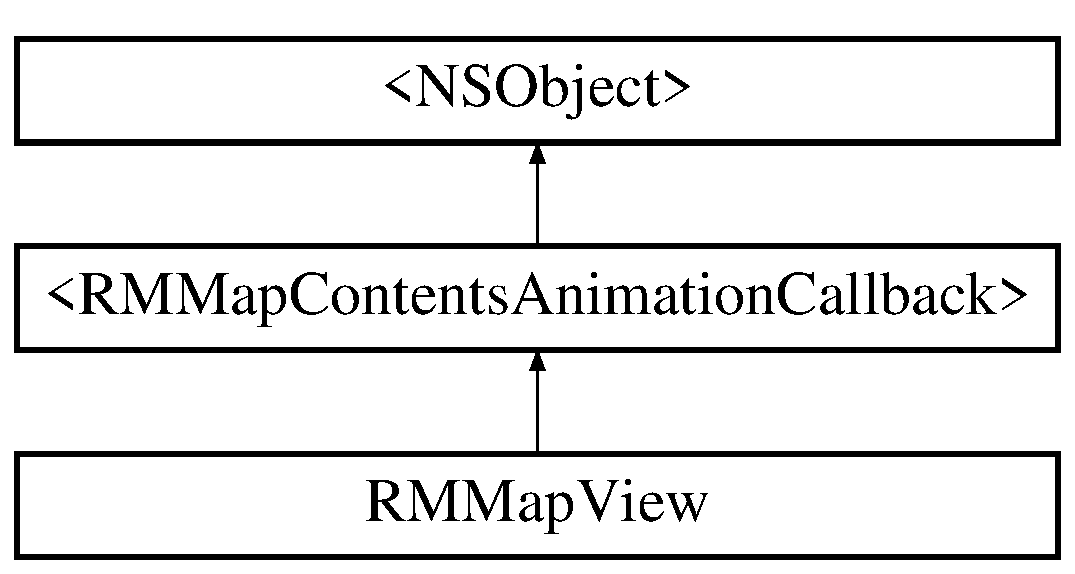
\includegraphics[height=3.000000cm]{protocol_r_m_map_contents_animation_callback-p}
\end{center}
\end{figure}
\subsection*{Instance Methods}
\begin{DoxyCompactItemize}
\item 
(void) -\/ \hyperlink{protocol_r_m_map_contents_animation_callback-p_afd3a55e53810bb11b843754ffa4d346d}{animation\-Finished\-With\-Zoom\-Factor\-:near\-:}
\item 
(void) -\/ \hyperlink{protocol_r_m_map_contents_animation_callback-p_a404de1d6b9991d9daf716996b515ec6c}{animation\-Stepped}
\end{DoxyCompactItemize}


\subsection{Method Documentation}
\hypertarget{protocol_r_m_map_contents_animation_callback-p_afd3a55e53810bb11b843754ffa4d346d}{\index{R\-M\-Map\-Contents\-Animation\-Callback-\/p@{R\-M\-Map\-Contents\-Animation\-Callback-\/p}!animation\-Finished\-With\-Zoom\-Factor\-:near\-:@{animation\-Finished\-With\-Zoom\-Factor\-:near\-:}}
\index{animation\-Finished\-With\-Zoom\-Factor\-:near\-:@{animation\-Finished\-With\-Zoom\-Factor\-:near\-:}!RMMapContentsAnimationCallback-p@{R\-M\-Map\-Contents\-Animation\-Callback-\/p}}
\subsubsection[{animation\-Finished\-With\-Zoom\-Factor\-:near\-:}]{\setlength{\rightskip}{0pt plus 5cm}-\/ (void) animation\-Finished\-With\-Zoom\-Factor\-: 
\begin{DoxyParamCaption}
\item[{(float)}]{zoom\-Factor}
\item[{near:(C\-G\-Point)}]{p}
\end{DoxyParamCaption}
\hspace{0.3cm}{\ttfamily [optional]}}}\label{protocol_r_m_map_contents_animation_callback-p_afd3a55e53810bb11b843754ffa4d346d}


被 \hyperlink{interface_r_m_map_view_ab512cbaf772a0c0b6a8a8fb10f80d2b4}{R\-M\-Map\-View} 重载.



参考自 R\-M\-Map\-Contents\-::animated\-Zoom\-Step\-:.

\hypertarget{protocol_r_m_map_contents_animation_callback-p_a404de1d6b9991d9daf716996b515ec6c}{\index{R\-M\-Map\-Contents\-Animation\-Callback-\/p@{R\-M\-Map\-Contents\-Animation\-Callback-\/p}!animation\-Stepped@{animation\-Stepped}}
\index{animation\-Stepped@{animation\-Stepped}!RMMapContentsAnimationCallback-p@{R\-M\-Map\-Contents\-Animation\-Callback-\/p}}
\subsubsection[{animation\-Stepped}]{\setlength{\rightskip}{0pt plus 5cm}-\/ (void) animation\-Stepped 
\begin{DoxyParamCaption}
{}
\end{DoxyParamCaption}
\hspace{0.3cm}{\ttfamily [optional]}}}\label{protocol_r_m_map_contents_animation_callback-p_a404de1d6b9991d9daf716996b515ec6c}


被 \hyperlink{interface_r_m_map_view_a795716de54229787251beb8957477905}{R\-M\-Map\-View} 重载.



参考自 R\-M\-Map\-Contents\-::animated\-Zoom\-Step\-:.



该协议的文档由以下文件生成\-:\begin{DoxyCompactItemize}
\item 
Map/\hyperlink{_r_m_map_contents_8h}{R\-M\-Map\-Contents.\-h}\end{DoxyCompactItemize}

\hypertarget{protocol_r_m_map_contents_facade-p}{\section{$<$R\-M\-Map\-Contents\-Facade$>$协议 参考}
\label{protocol_r_m_map_contents_facade-p}\index{$<$\-R\-M\-Map\-Contents\-Facade$>$@{$<$\-R\-M\-Map\-Contents\-Facade$>$}}
}


Appears to be the methods actually implemented by \hyperlink{interface_r_m_map_contents}{R\-M\-Map\-Contents}, but generally invoked on \hyperlink{interface_r_m_map_view}{R\-M\-Map\-View}, and forwarded to the contents object.  




{\ttfamily \#import $<$R\-M\-Map\-Contents.\-h$>$}

类 $<$R\-M\-Map\-Contents\-Facade$>$ 继承关系图\-:\begin{figure}[H]
\begin{center}
\leavevmode
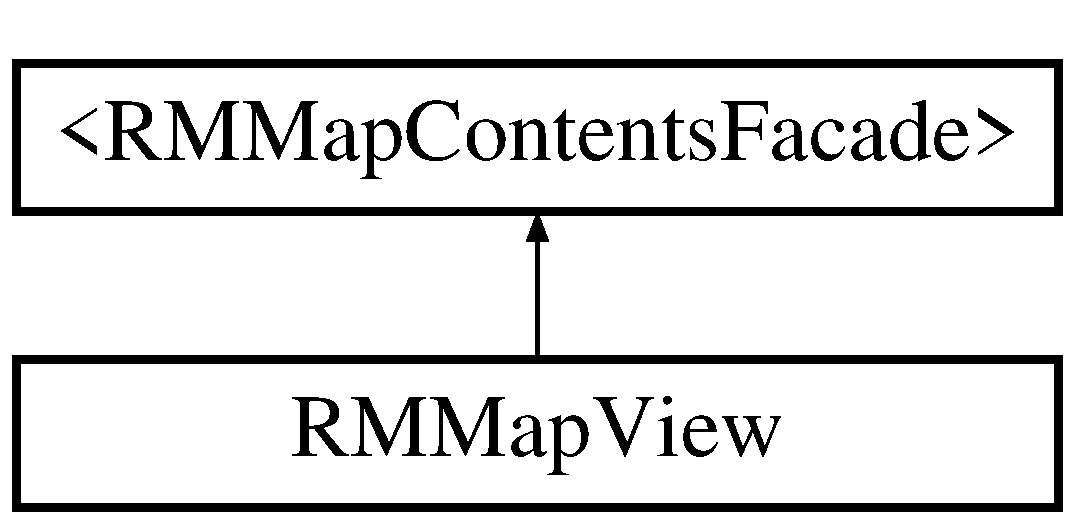
\includegraphics[height=2.000000cm]{protocol_r_m_map_contents_facade-p}
\end{center}
\end{figure}
\subsection*{Instance Methods}
\begin{DoxyCompactItemize}
\item 
(void) -\/ \hyperlink{protocol_r_m_map_contents_facade-p_a87677eea4a25861fe62cc2f8abb9842c}{adjust\-Map\-Placement\-With\-Scale\-:}
\item 
(float) -\/ \hyperlink{protocol_r_m_map_contents_facade-p_ac8f6ec5e5da36d4325cb4bda73a56b4a}{adjust\-Zoom\-For\-Bounding\-Mask\-:}
\item 
(\hyperlink{struct_r_m_spherical_trapezium}{R\-M\-Spherical\-Trapezium}) -\/ \hyperlink{protocol_r_m_map_contents_facade-p_a3472abc47e5dc6ebde858df2e168f9f1}{latitude\-Longitude\-Bounding\-Box\-For\-:}
\item 
(\hyperlink{struct_r_m_spherical_trapezium}{R\-M\-Spherical\-Trapezium}) -\/ \hyperlink{protocol_r_m_map_contents_facade-p_a45d3b80e0d26fdce5ec55edd29df8aed}{latitude\-Longitude\-Bounding\-Box\-For\-Screen}
\item 
(C\-G\-Point) -\/ \hyperlink{protocol_r_m_map_contents_facade-p_abe6c43a3535d4f793dd992f4e4202c74}{lat\-Long\-To\-Pixel\-:}
\item 
(C\-G\-Point) -\/ \hyperlink{protocol_r_m_map_contents_facade-p_a89f7b022d8955d82efa669f31eb9056a}{lat\-Long\-To\-Pixel\-:with\-Meters\-Per\-Pixel\-:}
\item 
(void) -\/ \hyperlink{protocol_r_m_map_contents_facade-p_a229f6bcfb540a9afb2f1620c2e79fcb2}{move\-By\-:}
\item 
(void) -\/ \hyperlink{protocol_r_m_map_contents_facade-p_afab5c65cfffa2209a44ed73962218589}{move\-To\-Lat\-Long\-:}
\item 
(void) -\/ \hyperlink{protocol_r_m_map_contents_facade-p_a2cdc6dc414cefda8f1616dd6572d5627}{move\-To\-Projected\-Point\-:}
\item 
(C\-L\-Location\-Coordinate2\-D) -\/ \hyperlink{protocol_r_m_map_contents_facade-p_a9e67a602bc0158b14610d0648640b856}{pixel\-To\-Lat\-Long\-:}
\item 
(C\-L\-Location\-Coordinate2\-D) -\/ \hyperlink{protocol_r_m_map_contents_facade-p_a6d1204e38b5879349d12f6fc57e93001}{pixel\-To\-Lat\-Long\-:with\-Meters\-Per\-Pixel\-:}
\item 
(void) -\/ \hyperlink{protocol_r_m_map_contents_facade-p_a862d9e91572a50e6ddb76a9985fdee05}{tiles\-Updated\-Region\-:}
\item 
(void) -\/ \hyperlink{protocol_r_m_map_contents_facade-p_af9a47536d397223358380cac31c960e1}{zoom\-By\-Factor\-:near\-:}
\item 
(void) -\/ \hyperlink{protocol_r_m_map_contents_facade-p_adbcb106790b92819764375c1f0deb77b}{zoom\-By\-Factor\-:near\-:animated\-:}
\item 
(void) -\/ \hyperlink{protocol_r_m_map_contents_facade-p_ae428e14027ddbb7e01fbd76e12b9563b}{zoom\-In\-To\-Next\-Native\-Zoom\-At\-:}
\item 
(void) -\/ \hyperlink{protocol_r_m_map_contents_facade-p_a6789cd20384edead12a12c756b79d31a}{zoom\-In\-To\-Next\-Native\-Zoom\-At\-:animated\-:}
\item 
(void) -\/ \hyperlink{protocol_r_m_map_contents_facade-p_a789f690bbc442baec16cf38d1341cc49}{zoom\-Out\-To\-Next\-Native\-Zoom\-At\-:}
\item 
(void) -\/ \hyperlink{protocol_r_m_map_contents_facade-p_adb9ae6c8f8b4c4e8168adb0ddac9a768}{zoom\-Out\-To\-Next\-Native\-Zoom\-At\-:animated\-:}
\item 
(void) -\/ \hyperlink{protocol_r_m_map_contents_facade-p_a95002f376d4c057ed69c39a33d738698}{zoom\-With\-Lat\-Lng\-Bounds\-North\-East\-:\-South\-West\-:}
\item 
(void) -\/ \hyperlink{protocol_r_m_map_contents_facade-p_adac46282107bc99c884bcc1365845059}{zoom\-With\-R\-M\-Mercator\-Rect\-Bounds\-:}
\end{DoxyCompactItemize}


\subsection{详细描述}
Appears to be the methods actually implemented by \hyperlink{interface_r_m_map_contents}{R\-M\-Map\-Contents}, but generally invoked on \hyperlink{interface_r_m_map_view}{R\-M\-Map\-View}, and forwarded to the contents object. 

\subsection{Method Documentation}
\hypertarget{protocol_r_m_map_contents_facade-p_a87677eea4a25861fe62cc2f8abb9842c}{\index{R\-M\-Map\-Contents\-Facade-\/p@{R\-M\-Map\-Contents\-Facade-\/p}!adjust\-Map\-Placement\-With\-Scale\-:@{adjust\-Map\-Placement\-With\-Scale\-:}}
\index{adjust\-Map\-Placement\-With\-Scale\-:@{adjust\-Map\-Placement\-With\-Scale\-:}!RMMapContentsFacade-p@{R\-M\-Map\-Contents\-Facade-\/p}}
\subsubsection[{adjust\-Map\-Placement\-With\-Scale\-:}]{\setlength{\rightskip}{0pt plus 5cm}-\/ (void) adjust\-Map\-Placement\-With\-Scale\-: 
\begin{DoxyParamCaption}
\item[{(float)}]{a\-Scale}
\end{DoxyParamCaption}
\hspace{0.3cm}{\ttfamily [optional]}}}\label{protocol_r_m_map_contents_facade-p_a87677eea4a25861fe62cc2f8abb9842c}
\hypertarget{protocol_r_m_map_contents_facade-p_ac8f6ec5e5da36d4325cb4bda73a56b4a}{\index{R\-M\-Map\-Contents\-Facade-\/p@{R\-M\-Map\-Contents\-Facade-\/p}!adjust\-Zoom\-For\-Bounding\-Mask\-:@{adjust\-Zoom\-For\-Bounding\-Mask\-:}}
\index{adjust\-Zoom\-For\-Bounding\-Mask\-:@{adjust\-Zoom\-For\-Bounding\-Mask\-:}!RMMapContentsFacade-p@{R\-M\-Map\-Contents\-Facade-\/p}}
\subsubsection[{adjust\-Zoom\-For\-Bounding\-Mask\-:}]{\setlength{\rightskip}{0pt plus 5cm}-\/ (float) adjust\-Zoom\-For\-Bounding\-Mask\-: 
\begin{DoxyParamCaption}
\item[{(float)}]{zoom\-Factor}
\end{DoxyParamCaption}
\hspace{0.3cm}{\ttfamily [optional]}}}\label{protocol_r_m_map_contents_facade-p_ac8f6ec5e5da36d4325cb4bda73a56b4a}


参考自 R\-M\-Map\-View\-::zoom\-By\-Factor\-:near\-:animated\-:.

\hypertarget{protocol_r_m_map_contents_facade-p_a3472abc47e5dc6ebde858df2e168f9f1}{\index{R\-M\-Map\-Contents\-Facade-\/p@{R\-M\-Map\-Contents\-Facade-\/p}!latitude\-Longitude\-Bounding\-Box\-For\-:@{latitude\-Longitude\-Bounding\-Box\-For\-:}}
\index{latitude\-Longitude\-Bounding\-Box\-For\-:@{latitude\-Longitude\-Bounding\-Box\-For\-:}!RMMapContentsFacade-p@{R\-M\-Map\-Contents\-Facade-\/p}}
\subsubsection[{latitude\-Longitude\-Bounding\-Box\-For\-:}]{\setlength{\rightskip}{0pt plus 5cm}-\/ ({\bf R\-M\-Spherical\-Trapezium}) latitude\-Longitude\-Bounding\-Box\-For\-: 
\begin{DoxyParamCaption}
\item[{(C\-G\-Rect)}]{rect}
\end{DoxyParamCaption}
\hspace{0.3cm}{\ttfamily [optional]}}}\label{protocol_r_m_map_contents_facade-p_a3472abc47e5dc6ebde858df2e168f9f1}
\begin{DoxyRefDesc}{弃用}
\item[\hyperlink{deprecated__deprecated000006}{弃用}]name change pending after 0.\-5 \end{DoxyRefDesc}
\hypertarget{protocol_r_m_map_contents_facade-p_a45d3b80e0d26fdce5ec55edd29df8aed}{\index{R\-M\-Map\-Contents\-Facade-\/p@{R\-M\-Map\-Contents\-Facade-\/p}!latitude\-Longitude\-Bounding\-Box\-For\-Screen@{latitude\-Longitude\-Bounding\-Box\-For\-Screen}}
\index{latitude\-Longitude\-Bounding\-Box\-For\-Screen@{latitude\-Longitude\-Bounding\-Box\-For\-Screen}!RMMapContentsFacade-p@{R\-M\-Map\-Contents\-Facade-\/p}}
\subsubsection[{latitude\-Longitude\-Bounding\-Box\-For\-Screen}]{\setlength{\rightskip}{0pt plus 5cm}-\/ ({\bf R\-M\-Spherical\-Trapezium}) latitude\-Longitude\-Bounding\-Box\-For\-Screen 
\begin{DoxyParamCaption}
{}
\end{DoxyParamCaption}
\hspace{0.3cm}{\ttfamily [optional]}}}\label{protocol_r_m_map_contents_facade-p_a45d3b80e0d26fdce5ec55edd29df8aed}
\begin{DoxyRefDesc}{弃用}
\item[\hyperlink{deprecated__deprecated000005}{弃用}]name change pending after 0.\-5 \end{DoxyRefDesc}
\hypertarget{protocol_r_m_map_contents_facade-p_abe6c43a3535d4f793dd992f4e4202c74}{\index{R\-M\-Map\-Contents\-Facade-\/p@{R\-M\-Map\-Contents\-Facade-\/p}!lat\-Long\-To\-Pixel\-:@{lat\-Long\-To\-Pixel\-:}}
\index{lat\-Long\-To\-Pixel\-:@{lat\-Long\-To\-Pixel\-:}!RMMapContentsFacade-p@{R\-M\-Map\-Contents\-Facade-\/p}}
\subsubsection[{lat\-Long\-To\-Pixel\-:}]{\setlength{\rightskip}{0pt plus 5cm}-\/ (C\-G\-Point) lat\-Long\-To\-Pixel\-: 
\begin{DoxyParamCaption}
\item[{(C\-L\-Location\-Coordinate2\-D)}]{latlong}
\end{DoxyParamCaption}
\hspace{0.3cm}{\ttfamily [optional]}}}\label{protocol_r_m_map_contents_facade-p_abe6c43a3535d4f793dd992f4e4202c74}


参考自 Route\-Me\-Tests\-::test\-Screen\-Coordinates\-Far\-East, Route\-Me\-Tests\-::test\-Screen\-Coordinates\-Far\-West , 以及 Route\-Me\-Tests\-::test\-Screen\-Coordinates\-Pacific\-Northwest.

\hypertarget{protocol_r_m_map_contents_facade-p_a89f7b022d8955d82efa669f31eb9056a}{\index{R\-M\-Map\-Contents\-Facade-\/p@{R\-M\-Map\-Contents\-Facade-\/p}!lat\-Long\-To\-Pixel\-:with\-Meters\-Per\-Pixel\-:@{lat\-Long\-To\-Pixel\-:with\-Meters\-Per\-Pixel\-:}}
\index{lat\-Long\-To\-Pixel\-:with\-Meters\-Per\-Pixel\-:@{lat\-Long\-To\-Pixel\-:with\-Meters\-Per\-Pixel\-:}!RMMapContentsFacade-p@{R\-M\-Map\-Contents\-Facade-\/p}}
\subsubsection[{lat\-Long\-To\-Pixel\-:with\-Meters\-Per\-Pixel\-:}]{\setlength{\rightskip}{0pt plus 5cm}-\/ (C\-G\-Point) {\bf lat\-Long\-To\-Pixel\-:} 
\begin{DoxyParamCaption}
\item[{(C\-L\-Location\-Coordinate2\-D)}]{latlong}
\item[{withMetersPerPixel:(float)}]{a\-Scale}
\end{DoxyParamCaption}
\hspace{0.3cm}{\ttfamily [optional]}}}\label{protocol_r_m_map_contents_facade-p_a89f7b022d8955d82efa669f31eb9056a}
\hypertarget{protocol_r_m_map_contents_facade-p_a229f6bcfb540a9afb2f1620c2e79fcb2}{\index{R\-M\-Map\-Contents\-Facade-\/p@{R\-M\-Map\-Contents\-Facade-\/p}!move\-By\-:@{move\-By\-:}}
\index{move\-By\-:@{move\-By\-:}!RMMapContentsFacade-p@{R\-M\-Map\-Contents\-Facade-\/p}}
\subsubsection[{move\-By\-:}]{\setlength{\rightskip}{0pt plus 5cm}-\/ (void) move\-By\-: 
\begin{DoxyParamCaption}
\item[{(C\-G\-Size)}]{delta}
\end{DoxyParamCaption}
\hspace{0.3cm}{\ttfamily [optional]}}}\label{protocol_r_m_map_contents_facade-p_a229f6bcfb540a9afb2f1620c2e79fcb2}


被 \hyperlink{interface_r_m_map_view_a27baf3f4a31aca87ce9f1a54437b1af0}{R\-M\-Map\-View} 重载.

\hypertarget{protocol_r_m_map_contents_facade-p_afab5c65cfffa2209a44ed73962218589}{\index{R\-M\-Map\-Contents\-Facade-\/p@{R\-M\-Map\-Contents\-Facade-\/p}!move\-To\-Lat\-Long\-:@{move\-To\-Lat\-Long\-:}}
\index{move\-To\-Lat\-Long\-:@{move\-To\-Lat\-Long\-:}!RMMapContentsFacade-p@{R\-M\-Map\-Contents\-Facade-\/p}}
\subsubsection[{move\-To\-Lat\-Long\-:}]{\setlength{\rightskip}{0pt plus 5cm}-\/ (void) move\-To\-Lat\-Long\-: 
\begin{DoxyParamCaption}
\item[{(C\-L\-Location\-Coordinate2\-D)}]{latlong}
\end{DoxyParamCaption}
\hspace{0.3cm}{\ttfamily [optional]}}}\label{protocol_r_m_map_contents_facade-p_afab5c65cfffa2209a44ed73962218589}


被 \hyperlink{interface_r_m_map_view_a1097238683168693264f3f1fd0e69f80}{R\-M\-Map\-View} 重载.

\hypertarget{protocol_r_m_map_contents_facade-p_a2cdc6dc414cefda8f1616dd6572d5627}{\index{R\-M\-Map\-Contents\-Facade-\/p@{R\-M\-Map\-Contents\-Facade-\/p}!move\-To\-Projected\-Point\-:@{move\-To\-Projected\-Point\-:}}
\index{move\-To\-Projected\-Point\-:@{move\-To\-Projected\-Point\-:}!RMMapContentsFacade-p@{R\-M\-Map\-Contents\-Facade-\/p}}
\subsubsection[{move\-To\-Projected\-Point\-:}]{\setlength{\rightskip}{0pt plus 5cm}-\/ (void) move\-To\-Projected\-Point\-: 
\begin{DoxyParamCaption}
\item[{({\bf R\-M\-Projected\-Point})}]{a\-Point}
\end{DoxyParamCaption}
\hspace{0.3cm}{\ttfamily [optional]}}}\label{protocol_r_m_map_contents_facade-p_a2cdc6dc414cefda8f1616dd6572d5627}


被 \hyperlink{interface_r_m_map_view_a7a576fb939de0ccc3e50f5f92ef9718d}{R\-M\-Map\-View} 重载.

\hypertarget{protocol_r_m_map_contents_facade-p_a9e67a602bc0158b14610d0648640b856}{\index{R\-M\-Map\-Contents\-Facade-\/p@{R\-M\-Map\-Contents\-Facade-\/p}!pixel\-To\-Lat\-Long\-:@{pixel\-To\-Lat\-Long\-:}}
\index{pixel\-To\-Lat\-Long\-:@{pixel\-To\-Lat\-Long\-:}!RMMapContentsFacade-p@{R\-M\-Map\-Contents\-Facade-\/p}}
\subsubsection[{pixel\-To\-Lat\-Long\-:}]{\setlength{\rightskip}{0pt plus 5cm}-\/ (C\-L\-Location\-Coordinate2\-D) pixel\-To\-Lat\-Long\-: 
\begin{DoxyParamCaption}
\item[{(C\-G\-Point)}]{a\-Pixel}
\end{DoxyParamCaption}
\hspace{0.3cm}{\ttfamily [optional]}}}\label{protocol_r_m_map_contents_facade-p_a9e67a602bc0158b14610d0648640b856}
\hypertarget{protocol_r_m_map_contents_facade-p_a6d1204e38b5879349d12f6fc57e93001}{\index{R\-M\-Map\-Contents\-Facade-\/p@{R\-M\-Map\-Contents\-Facade-\/p}!pixel\-To\-Lat\-Long\-:with\-Meters\-Per\-Pixel\-:@{pixel\-To\-Lat\-Long\-:with\-Meters\-Per\-Pixel\-:}}
\index{pixel\-To\-Lat\-Long\-:with\-Meters\-Per\-Pixel\-:@{pixel\-To\-Lat\-Long\-:with\-Meters\-Per\-Pixel\-:}!RMMapContentsFacade-p@{R\-M\-Map\-Contents\-Facade-\/p}}
\subsubsection[{pixel\-To\-Lat\-Long\-:with\-Meters\-Per\-Pixel\-:}]{\setlength{\rightskip}{0pt plus 5cm}-\/ (C\-L\-Location\-Coordinate2\-D) {\bf pixel\-To\-Lat\-Long\-:} 
\begin{DoxyParamCaption}
\item[{(C\-G\-Point)}]{a\-Pixel}
\item[{withMetersPerPixel:(float)}]{a\-Scale}
\end{DoxyParamCaption}
\hspace{0.3cm}{\ttfamily [optional]}}}\label{protocol_r_m_map_contents_facade-p_a6d1204e38b5879349d12f6fc57e93001}
\hypertarget{protocol_r_m_map_contents_facade-p_a862d9e91572a50e6ddb76a9985fdee05}{\index{R\-M\-Map\-Contents\-Facade-\/p@{R\-M\-Map\-Contents\-Facade-\/p}!tiles\-Updated\-Region\-:@{tiles\-Updated\-Region\-:}}
\index{tiles\-Updated\-Region\-:@{tiles\-Updated\-Region\-:}!RMMapContentsFacade-p@{R\-M\-Map\-Contents\-Facade-\/p}}
\subsubsection[{tiles\-Updated\-Region\-:}]{\setlength{\rightskip}{0pt plus 5cm}-\/ (void) tiles\-Updated\-Region\-: 
\begin{DoxyParamCaption}
\item[{(C\-G\-Rect)}]{region}
\end{DoxyParamCaption}
\hspace{0.3cm}{\ttfamily [optional]}}}\label{protocol_r_m_map_contents_facade-p_a862d9e91572a50e6ddb76a9985fdee05}
\hypertarget{protocol_r_m_map_contents_facade-p_af9a47536d397223358380cac31c960e1}{\index{R\-M\-Map\-Contents\-Facade-\/p@{R\-M\-Map\-Contents\-Facade-\/p}!zoom\-By\-Factor\-:near\-:@{zoom\-By\-Factor\-:near\-:}}
\index{zoom\-By\-Factor\-:near\-:@{zoom\-By\-Factor\-:near\-:}!RMMapContentsFacade-p@{R\-M\-Map\-Contents\-Facade-\/p}}
\subsubsection[{zoom\-By\-Factor\-:near\-:}]{\setlength{\rightskip}{0pt plus 5cm}-\/ (void) zoom\-By\-Factor\-: 
\begin{DoxyParamCaption}
\item[{(float)}]{zoom\-Factor}
\item[{near:(C\-G\-Point)}]{center}
\end{DoxyParamCaption}
\hspace{0.3cm}{\ttfamily [optional]}}}\label{protocol_r_m_map_contents_facade-p_af9a47536d397223358380cac31c960e1}


被 \hyperlink{interface_r_m_map_view_a6003bcb4479e3ca7f2500db18f7ee8e8}{R\-M\-Map\-View} 重载.

\hypertarget{protocol_r_m_map_contents_facade-p_adbcb106790b92819764375c1f0deb77b}{\index{R\-M\-Map\-Contents\-Facade-\/p@{R\-M\-Map\-Contents\-Facade-\/p}!zoom\-By\-Factor\-:near\-:animated\-:@{zoom\-By\-Factor\-:near\-:animated\-:}}
\index{zoom\-By\-Factor\-:near\-:animated\-:@{zoom\-By\-Factor\-:near\-:animated\-:}!RMMapContentsFacade-p@{R\-M\-Map\-Contents\-Facade-\/p}}
\subsubsection[{zoom\-By\-Factor\-:near\-:animated\-:}]{\setlength{\rightskip}{0pt plus 5cm}-\/ (void) zoom\-By\-Factor\-: 
\begin{DoxyParamCaption}
\item[{(float)}]{zoom\-Factor}
\item[{near:(C\-G\-Point)}]{center}
\item[{animated:(B\-O\-O\-L)}]{animated}
\end{DoxyParamCaption}
\hspace{0.3cm}{\ttfamily [optional]}}}\label{protocol_r_m_map_contents_facade-p_adbcb106790b92819764375c1f0deb77b}


被 \hyperlink{interface_r_m_map_view_a30bd6e4766b3bc224a6e214bb06ec8ca}{R\-M\-Map\-View} 重载.

\hypertarget{protocol_r_m_map_contents_facade-p_ae428e14027ddbb7e01fbd76e12b9563b}{\index{R\-M\-Map\-Contents\-Facade-\/p@{R\-M\-Map\-Contents\-Facade-\/p}!zoom\-In\-To\-Next\-Native\-Zoom\-At\-:@{zoom\-In\-To\-Next\-Native\-Zoom\-At\-:}}
\index{zoom\-In\-To\-Next\-Native\-Zoom\-At\-:@{zoom\-In\-To\-Next\-Native\-Zoom\-At\-:}!RMMapContentsFacade-p@{R\-M\-Map\-Contents\-Facade-\/p}}
\subsubsection[{zoom\-In\-To\-Next\-Native\-Zoom\-At\-:}]{\setlength{\rightskip}{0pt plus 5cm}-\/ (void) zoom\-In\-To\-Next\-Native\-Zoom\-At\-: 
\begin{DoxyParamCaption}
\item[{(C\-G\-Point)}]{pivot}
\end{DoxyParamCaption}
\hspace{0.3cm}{\ttfamily [optional]}}}\label{protocol_r_m_map_contents_facade-p_ae428e14027ddbb7e01fbd76e12b9563b}
\hypertarget{protocol_r_m_map_contents_facade-p_a6789cd20384edead12a12c756b79d31a}{\index{R\-M\-Map\-Contents\-Facade-\/p@{R\-M\-Map\-Contents\-Facade-\/p}!zoom\-In\-To\-Next\-Native\-Zoom\-At\-:animated\-:@{zoom\-In\-To\-Next\-Native\-Zoom\-At\-:animated\-:}}
\index{zoom\-In\-To\-Next\-Native\-Zoom\-At\-:animated\-:@{zoom\-In\-To\-Next\-Native\-Zoom\-At\-:animated\-:}!RMMapContentsFacade-p@{R\-M\-Map\-Contents\-Facade-\/p}}
\subsubsection[{zoom\-In\-To\-Next\-Native\-Zoom\-At\-:animated\-:}]{\setlength{\rightskip}{0pt plus 5cm}-\/ (void) {\bf zoom\-In\-To\-Next\-Native\-Zoom\-At\-:} 
\begin{DoxyParamCaption}
\item[{(C\-G\-Point)}]{pivot}
\item[{animated:(B\-O\-O\-L)}]{animated}
\end{DoxyParamCaption}
\hspace{0.3cm}{\ttfamily [optional]}}}\label{protocol_r_m_map_contents_facade-p_a6789cd20384edead12a12c756b79d31a}
\hypertarget{protocol_r_m_map_contents_facade-p_a789f690bbc442baec16cf38d1341cc49}{\index{R\-M\-Map\-Contents\-Facade-\/p@{R\-M\-Map\-Contents\-Facade-\/p}!zoom\-Out\-To\-Next\-Native\-Zoom\-At\-:@{zoom\-Out\-To\-Next\-Native\-Zoom\-At\-:}}
\index{zoom\-Out\-To\-Next\-Native\-Zoom\-At\-:@{zoom\-Out\-To\-Next\-Native\-Zoom\-At\-:}!RMMapContentsFacade-p@{R\-M\-Map\-Contents\-Facade-\/p}}
\subsubsection[{zoom\-Out\-To\-Next\-Native\-Zoom\-At\-:}]{\setlength{\rightskip}{0pt plus 5cm}-\/ (void) zoom\-Out\-To\-Next\-Native\-Zoom\-At\-: 
\begin{DoxyParamCaption}
\item[{(C\-G\-Point)}]{pivot}
\end{DoxyParamCaption}
\hspace{0.3cm}{\ttfamily [optional]}}}\label{protocol_r_m_map_contents_facade-p_a789f690bbc442baec16cf38d1341cc49}
\hypertarget{protocol_r_m_map_contents_facade-p_adb9ae6c8f8b4c4e8168adb0ddac9a768}{\index{R\-M\-Map\-Contents\-Facade-\/p@{R\-M\-Map\-Contents\-Facade-\/p}!zoom\-Out\-To\-Next\-Native\-Zoom\-At\-:animated\-:@{zoom\-Out\-To\-Next\-Native\-Zoom\-At\-:animated\-:}}
\index{zoom\-Out\-To\-Next\-Native\-Zoom\-At\-:animated\-:@{zoom\-Out\-To\-Next\-Native\-Zoom\-At\-:animated\-:}!RMMapContentsFacade-p@{R\-M\-Map\-Contents\-Facade-\/p}}
\subsubsection[{zoom\-Out\-To\-Next\-Native\-Zoom\-At\-:animated\-:}]{\setlength{\rightskip}{0pt plus 5cm}-\/ (void) {\bf zoom\-Out\-To\-Next\-Native\-Zoom\-At\-:} 
\begin{DoxyParamCaption}
\item[{(C\-G\-Point)}]{pivot}
\item[{animated:(B\-O\-O\-L)}]{animated}
\end{DoxyParamCaption}
\hspace{0.3cm}{\ttfamily [optional]}}}\label{protocol_r_m_map_contents_facade-p_adb9ae6c8f8b4c4e8168adb0ddac9a768}
\hypertarget{protocol_r_m_map_contents_facade-p_a95002f376d4c057ed69c39a33d738698}{\index{R\-M\-Map\-Contents\-Facade-\/p@{R\-M\-Map\-Contents\-Facade-\/p}!zoom\-With\-Lat\-Lng\-Bounds\-North\-East\-:\-South\-West\-:@{zoom\-With\-Lat\-Lng\-Bounds\-North\-East\-:\-South\-West\-:}}
\index{zoom\-With\-Lat\-Lng\-Bounds\-North\-East\-:\-South\-West\-:@{zoom\-With\-Lat\-Lng\-Bounds\-North\-East\-:\-South\-West\-:}!RMMapContentsFacade-p@{R\-M\-Map\-Contents\-Facade-\/p}}
\subsubsection[{zoom\-With\-Lat\-Lng\-Bounds\-North\-East\-:\-South\-West\-:}]{\setlength{\rightskip}{0pt plus 5cm}-\/ (void) zoom\-With\-Lat\-Lng\-Bounds\-North\-East\-: 
\begin{DoxyParamCaption}
\item[{(C\-L\-Location\-Coordinate2\-D)}]{ne}
\item[{SouthWest:(C\-L\-Location\-Coordinate2\-D)}]{se}
\end{DoxyParamCaption}
\hspace{0.3cm}{\ttfamily [optional]}}}\label{protocol_r_m_map_contents_facade-p_a95002f376d4c057ed69c39a33d738698}
\hypertarget{protocol_r_m_map_contents_facade-p_adac46282107bc99c884bcc1365845059}{\index{R\-M\-Map\-Contents\-Facade-\/p@{R\-M\-Map\-Contents\-Facade-\/p}!zoom\-With\-R\-M\-Mercator\-Rect\-Bounds\-:@{zoom\-With\-R\-M\-Mercator\-Rect\-Bounds\-:}}
\index{zoom\-With\-R\-M\-Mercator\-Rect\-Bounds\-:@{zoom\-With\-R\-M\-Mercator\-Rect\-Bounds\-:}!RMMapContentsFacade-p@{R\-M\-Map\-Contents\-Facade-\/p}}
\subsubsection[{zoom\-With\-R\-M\-Mercator\-Rect\-Bounds\-:}]{\setlength{\rightskip}{0pt plus 5cm}-\/ (void) zoom\-With\-R\-M\-Mercator\-Rect\-Bounds\-: 
\begin{DoxyParamCaption}
\item[{({\bf R\-M\-Projected\-Rect})}]{bounds}
\end{DoxyParamCaption}
\hspace{0.3cm}{\ttfamily [optional]}}}\label{protocol_r_m_map_contents_facade-p_adac46282107bc99c884bcc1365845059}


该协议的文档由以下文件生成\-:\begin{DoxyCompactItemize}
\item 
Map/\hyperlink{_r_m_map_contents_8h}{R\-M\-Map\-Contents.\-h}\end{DoxyCompactItemize}

\hypertarget{interface_r_m_map_layer}{\section{R\-M\-Map\-Layer类 参考}
\label{interface_r_m_map_layer}\index{R\-M\-Map\-Layer@{R\-M\-Map\-Layer}}
}


{\ttfamily \#import $<$R\-M\-Map\-Layer.\-h$>$}

类 R\-M\-Map\-Layer 继承关系图\-:\begin{figure}[H]
\begin{center}
\leavevmode
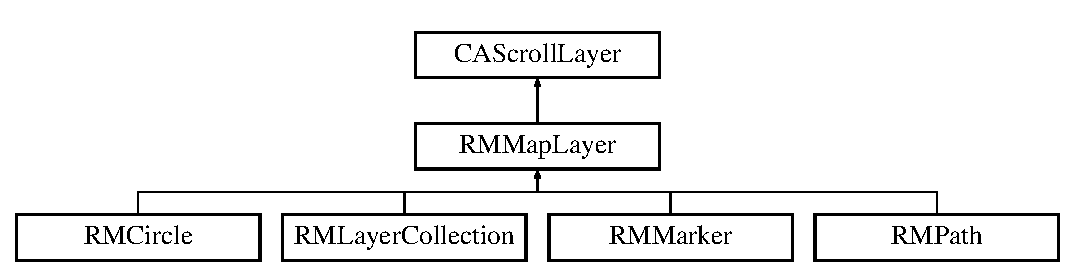
\includegraphics[height=3.000000cm]{interface_r_m_map_layer}
\end{center}
\end{figure}
\subsection*{Instance Methods}
\begin{DoxyCompactItemize}
\item 
(id$<$ C\-A\-Action $>$) -\/ \hyperlink{interface_r_m_map_layer_a28e0dabc0cf8638c6d26358354f4fcf8}{action\-For\-Key\-:}{\ttfamily  \mbox{[}implementation\mbox{]}}
\item 
(id) -\/ \hyperlink{interface_r_m_map_layer_a0ef1b877235bcaedb2929dae3bd92750}{init}{\ttfamily  \mbox{[}implementation\mbox{]}}
\item 
(id) -\/ \hyperlink{interface_r_m_map_layer_aa32c5f5b5e5d2723763780b9ccbabce8}{init\-With\-Layer\-:}{\ttfamily  \mbox{[}implementation\mbox{]}}
\item 
(void) -\/ \hyperlink{interface_r_m_map_layer_ac960944a80c596eb918531cf63c54c11}{move\-By\-:}
\item 
(void) -\/ \hyperlink{interface_r_m_map_layer_ae0e1f8c364aaca4ac39766fe14bbba07}{zoom\-By\-Factor\-:near\-:}
\end{DoxyCompactItemize}


\subsection{Method Documentation}
\hypertarget{interface_r_m_map_layer_a28e0dabc0cf8638c6d26358354f4fcf8}{\index{R\-M\-Map\-Layer@{R\-M\-Map\-Layer}!action\-For\-Key\-:@{action\-For\-Key\-:}}
\index{action\-For\-Key\-:@{action\-For\-Key\-:}!RMMapLayer@{R\-M\-Map\-Layer}}
\subsubsection[{action\-For\-Key\-:}]{\setlength{\rightskip}{0pt plus 5cm}-\/ (id$<$ C\-A\-Action $>$) action\-For\-Key\-: 
\begin{DoxyParamCaption}
\item[{(N\-S\-String $\ast$)}]{key}
\end{DoxyParamCaption}
\hspace{0.3cm}{\ttfamily [implementation]}}}\label{interface_r_m_map_layer_a28e0dabc0cf8638c6d26358354f4fcf8}
\begin{DoxyRefDesc}{Bug}
\item[\hyperlink{bug__bug000018}{Bug}]why return nil for the \char`\"{}position\char`\"{} and \char`\"{}bounds\char`\"{} action\-For\-Key? Does this do anything besides block Core Animation? \end{DoxyRefDesc}


被 \hyperlink{interface_r_m_path_aeff4f90d5d01092fd310a0b52d3c9d1c}{R\-M\-Path} 重载.

\hypertarget{interface_r_m_map_layer_a0ef1b877235bcaedb2929dae3bd92750}{\index{R\-M\-Map\-Layer@{R\-M\-Map\-Layer}!init@{init}}
\index{init@{init}!RMMapLayer@{R\-M\-Map\-Layer}}
\subsubsection[{init}]{\setlength{\rightskip}{0pt plus 5cm}-\/ (id) init 
\begin{DoxyParamCaption}
{}
\end{DoxyParamCaption}
\hspace{0.3cm}{\ttfamily [implementation]}}}\label{interface_r_m_map_layer_a0ef1b877235bcaedb2929dae3bd92750}


被 \hyperlink{interface_r_m_marker_ae896ffbfa063f34d49741f540b3f9201}{R\-M\-Marker} 重载.



参考自 R\-M\-Layer\-Collection\-::init\-For\-Contents\-:, R\-M\-Path\-::init\-With\-Contents\-: , 以及 R\-M\-Circle\-::init\-With\-Contents\-:radius\-In\-Meters\-:lat\-Long\-:.

\hypertarget{interface_r_m_map_layer_aa32c5f5b5e5d2723763780b9ccbabce8}{\index{R\-M\-Map\-Layer@{R\-M\-Map\-Layer}!init\-With\-Layer\-:@{init\-With\-Layer\-:}}
\index{init\-With\-Layer\-:@{init\-With\-Layer\-:}!RMMapLayer@{R\-M\-Map\-Layer}}
\subsubsection[{init\-With\-Layer\-:}]{\setlength{\rightskip}{0pt plus 5cm}-\/ (id) init\-With\-Layer\-: 
\begin{DoxyParamCaption}
\item[{(id)}]{layer}
\end{DoxyParamCaption}
\hspace{0.3cm}{\ttfamily [implementation]}}}\label{interface_r_m_map_layer_aa32c5f5b5e5d2723763780b9ccbabce8}
\hypertarget{interface_r_m_map_layer_ac960944a80c596eb918531cf63c54c11}{\index{R\-M\-Map\-Layer@{R\-M\-Map\-Layer}!move\-By\-:@{move\-By\-:}}
\index{move\-By\-:@{move\-By\-:}!RMMapLayer@{R\-M\-Map\-Layer}}
\subsubsection[{move\-By\-:}]{\setlength{\rightskip}{0pt plus 5cm}-\/ (void) move\-By\-: 
\begin{DoxyParamCaption}
\item[{(C\-G\-Size)}]{delta}
\end{DoxyParamCaption}
}}\label{interface_r_m_map_layer_ac960944a80c596eb918531cf63c54c11}


被 \hyperlink{interface_r_m_circle_ae75b2ad3001e194c07a13b53a2486871}{R\-M\-Circle}, \hyperlink{interface_r_m_marker_a96b0d02976d98b17a2d8383d9cb4c807}{R\-M\-Marker}, \hyperlink{interface_r_m_layer_collection_aea4e071b3b6841f2892ff7dde0f737e6}{R\-M\-Layer\-Collection} , 以及 \hyperlink{interface_r_m_path_aa51fa75ed859403de65279c357720646}{R\-M\-Path} 重载.



参考自 R\-M\-Path\-::move\-By\-:, R\-M\-Marker\-::move\-By\-: , 以及 R\-M\-Circle\-::move\-By\-:.

\hypertarget{interface_r_m_map_layer_ae0e1f8c364aaca4ac39766fe14bbba07}{\index{R\-M\-Map\-Layer@{R\-M\-Map\-Layer}!zoom\-By\-Factor\-:near\-:@{zoom\-By\-Factor\-:near\-:}}
\index{zoom\-By\-Factor\-:near\-:@{zoom\-By\-Factor\-:near\-:}!RMMapLayer@{R\-M\-Map\-Layer}}
\subsubsection[{zoom\-By\-Factor\-:near\-:}]{\setlength{\rightskip}{0pt plus 5cm}-\/ (void) zoom\-By\-Factor\-: 
\begin{DoxyParamCaption}
\item[{(float)}]{zoom\-Factor}
\item[{near:(C\-G\-Point)}]{center}
\end{DoxyParamCaption}
}}\label{interface_r_m_map_layer_ae0e1f8c364aaca4ac39766fe14bbba07}


被 \hyperlink{interface_r_m_circle_ad1cd9f88068ff39d6000f2bf9816cc2b}{R\-M\-Circle}, \hyperlink{interface_r_m_marker_ad98fa242aceef563743c13963d8a79ca}{R\-M\-Marker} , 以及 \hyperlink{interface_r_m_layer_collection_ade8dc9cb544571522ee47b35e124ac8e}{R\-M\-Layer\-Collection} 重载.



参考自 R\-M\-Circle\-::zoom\-By\-Factor\-:near\-:.



该类的文档由以下文件生成\-:\begin{DoxyCompactItemize}
\item 
Map/\hyperlink{_r_m_map_layer_8h}{R\-M\-Map\-Layer.\-h}\item 
Map/\hyperlink{_r_m_map_layer_8m}{R\-M\-Map\-Layer.\-m}\end{DoxyCompactItemize}

\hypertarget{interface_r_m_map_quest_o_s_m_source}{\section{R\-M\-Map\-Quest\-O\-S\-M\-Source类 参考}
\label{interface_r_m_map_quest_o_s_m_source}\index{R\-M\-Map\-Quest\-O\-S\-M\-Source@{R\-M\-Map\-Quest\-O\-S\-M\-Source}}
}


Subclass of \hyperlink{interface_r_m_abstract_mercator_web_source}{R\-M\-Abstract\-Mercator\-Web\-Source} for access to Map\-Quest's version of Open\-Street\-Map.  




{\ttfamily \#import $<$R\-M\-Map\-Quest\-O\-S\-M\-Source.\-h$>$}

类 R\-M\-Map\-Quest\-O\-S\-M\-Source 继承关系图\-:\begin{figure}[H]
\begin{center}
\leavevmode
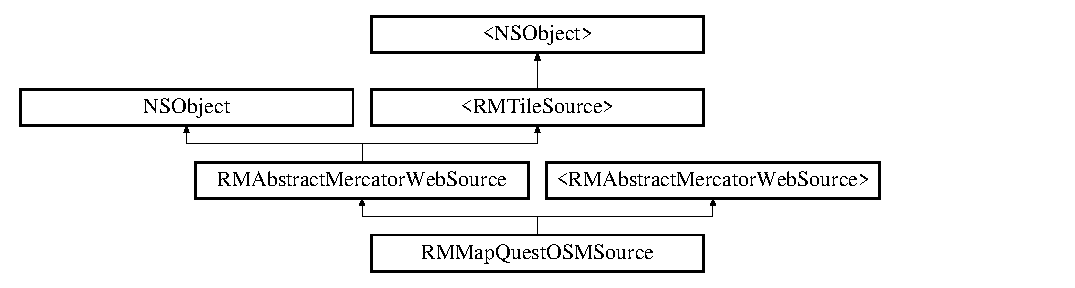
\includegraphics[height=3.425076cm]{interface_r_m_map_quest_o_s_m_source}
\end{center}
\end{figure}
\subsection*{Instance Methods}
\begin{DoxyCompactItemize}
\item 
(id) -\/ \hyperlink{interface_r_m_map_quest_o_s_m_source_aecd8d0a7ca60bc224ee43f8ad933fb1b}{init}{\ttfamily  \mbox{[}implementation\mbox{]}}
\item 
(N\-S\-String $\ast$) -\/ \hyperlink{interface_r_m_map_quest_o_s_m_source_a42722a15d1f14e114d2f4cd8de4010d6}{long\-Attribution}{\ttfamily  \mbox{[}implementation\mbox{]}}
\item 
(N\-S\-String $\ast$) -\/ \hyperlink{interface_r_m_map_quest_o_s_m_source_ab56b7a7914bb63cbec37f5e0cf556efd}{long\-Description}{\ttfamily  \mbox{[}implementation\mbox{]}}
\item 
(N\-S\-String $\ast$) -\/ \hyperlink{interface_r_m_map_quest_o_s_m_source_a14a58e74d28b38df3c93dfae7a7f6633}{short\-Attribution}{\ttfamily  \mbox{[}implementation\mbox{]}}
\item 
(N\-S\-String $\ast$) -\/ \hyperlink{interface_r_m_map_quest_o_s_m_source_adb22b17b97840aa7bc2170e896b464d9}{short\-Name}{\ttfamily  \mbox{[}implementation\mbox{]}}
\item 
(N\-S\-String $\ast$) -\/ \hyperlink{interface_r_m_map_quest_o_s_m_source_afb62c2d80e8f350ff3f1049f63e76b3b}{tile\-U\-R\-L\-:}{\ttfamily  \mbox{[}implementation\mbox{]}}
\item 
(N\-S\-String $\ast$) -\/ \hyperlink{interface_r_m_map_quest_o_s_m_source_ac5f1fbdc160544d60e9706b4e8e0c6a5}{unique\-Tilecache\-Key}{\ttfamily  \mbox{[}implementation\mbox{]}}
\end{DoxyCompactItemize}
\subsection*{额外继承的成员函数}


\subsection{详细描述}
Subclass of \hyperlink{interface_r_m_abstract_mercator_web_source}{R\-M\-Abstract\-Mercator\-Web\-Source} for access to Map\-Quest's version of Open\-Street\-Map. 

Provides key-\/based access to tiles from Map\-Quest project. 

\subsection{Method Documentation}
\hypertarget{interface_r_m_map_quest_o_s_m_source_aecd8d0a7ca60bc224ee43f8ad933fb1b}{\index{R\-M\-Map\-Quest\-O\-S\-M\-Source@{R\-M\-Map\-Quest\-O\-S\-M\-Source}!init@{init}}
\index{init@{init}!RMMapQuestOSMSource@{R\-M\-Map\-Quest\-O\-S\-M\-Source}}
\subsubsection[{init}]{\setlength{\rightskip}{0pt plus 5cm}-\/ (id) init 
\begin{DoxyParamCaption}
{}
\end{DoxyParamCaption}
\hspace{0.3cm}{\ttfamily [implementation]}}}\label{interface_r_m_map_quest_o_s_m_source_aecd8d0a7ca60bc224ee43f8ad933fb1b}


重载 \hyperlink{interface_r_m_abstract_mercator_web_source_a88bc1ea00a789381d77ae50e0eaec732}{R\-M\-Abstract\-Mercator\-Web\-Source} .

\hypertarget{interface_r_m_map_quest_o_s_m_source_a42722a15d1f14e114d2f4cd8de4010d6}{\index{R\-M\-Map\-Quest\-O\-S\-M\-Source@{R\-M\-Map\-Quest\-O\-S\-M\-Source}!long\-Attribution@{long\-Attribution}}
\index{long\-Attribution@{long\-Attribution}!RMMapQuestOSMSource@{R\-M\-Map\-Quest\-O\-S\-M\-Source}}
\subsubsection[{long\-Attribution}]{\setlength{\rightskip}{0pt plus 5cm}-\/ (N\-S\-String $\ast$) long\-Attribution 
\begin{DoxyParamCaption}
{}
\end{DoxyParamCaption}
\hspace{0.3cm}{\ttfamily [implementation]}}}\label{interface_r_m_map_quest_o_s_m_source_a42722a15d1f14e114d2f4cd8de4010d6}


重载 \hyperlink{interface_r_m_abstract_mercator_web_source_a77313c2d697428dd994a6e0cf07a256f}{R\-M\-Abstract\-Mercator\-Web\-Source} .

\hypertarget{interface_r_m_map_quest_o_s_m_source_ab56b7a7914bb63cbec37f5e0cf556efd}{\index{R\-M\-Map\-Quest\-O\-S\-M\-Source@{R\-M\-Map\-Quest\-O\-S\-M\-Source}!long\-Description@{long\-Description}}
\index{long\-Description@{long\-Description}!RMMapQuestOSMSource@{R\-M\-Map\-Quest\-O\-S\-M\-Source}}
\subsubsection[{long\-Description}]{\setlength{\rightskip}{0pt plus 5cm}-\/ (N\-S\-String $\ast$) long\-Description 
\begin{DoxyParamCaption}
{}
\end{DoxyParamCaption}
\hspace{0.3cm}{\ttfamily [implementation]}}}\label{interface_r_m_map_quest_o_s_m_source_ab56b7a7914bb63cbec37f5e0cf556efd}


重载 \hyperlink{interface_r_m_abstract_mercator_web_source_a9c1c86280c6fa05e4e82502822fcfd10}{R\-M\-Abstract\-Mercator\-Web\-Source} .

\hypertarget{interface_r_m_map_quest_o_s_m_source_a14a58e74d28b38df3c93dfae7a7f6633}{\index{R\-M\-Map\-Quest\-O\-S\-M\-Source@{R\-M\-Map\-Quest\-O\-S\-M\-Source}!short\-Attribution@{short\-Attribution}}
\index{short\-Attribution@{short\-Attribution}!RMMapQuestOSMSource@{R\-M\-Map\-Quest\-O\-S\-M\-Source}}
\subsubsection[{short\-Attribution}]{\setlength{\rightskip}{0pt plus 5cm}-\/ (N\-S\-String $\ast$) short\-Attribution 
\begin{DoxyParamCaption}
{}
\end{DoxyParamCaption}
\hspace{0.3cm}{\ttfamily [implementation]}}}\label{interface_r_m_map_quest_o_s_m_source_a14a58e74d28b38df3c93dfae7a7f6633}


重载 \hyperlink{interface_r_m_abstract_mercator_web_source_a6be24cea169d058b5eefd7572bedc366}{R\-M\-Abstract\-Mercator\-Web\-Source} .

\hypertarget{interface_r_m_map_quest_o_s_m_source_adb22b17b97840aa7bc2170e896b464d9}{\index{R\-M\-Map\-Quest\-O\-S\-M\-Source@{R\-M\-Map\-Quest\-O\-S\-M\-Source}!short\-Name@{short\-Name}}
\index{short\-Name@{short\-Name}!RMMapQuestOSMSource@{R\-M\-Map\-Quest\-O\-S\-M\-Source}}
\subsubsection[{short\-Name}]{\setlength{\rightskip}{0pt plus 5cm}-\/ (N\-S\-String $\ast$) short\-Name 
\begin{DoxyParamCaption}
{}
\end{DoxyParamCaption}
\hspace{0.3cm}{\ttfamily [implementation]}}}\label{interface_r_m_map_quest_o_s_m_source_adb22b17b97840aa7bc2170e896b464d9}


重载 \hyperlink{interface_r_m_abstract_mercator_web_source_a3e6c6ef18250ce14317373db9df1fc85}{R\-M\-Abstract\-Mercator\-Web\-Source} .

\hypertarget{interface_r_m_map_quest_o_s_m_source_afb62c2d80e8f350ff3f1049f63e76b3b}{\index{R\-M\-Map\-Quest\-O\-S\-M\-Source@{R\-M\-Map\-Quest\-O\-S\-M\-Source}!tile\-U\-R\-L\-:@{tile\-U\-R\-L\-:}}
\index{tile\-U\-R\-L\-:@{tile\-U\-R\-L\-:}!RMMapQuestOSMSource@{R\-M\-Map\-Quest\-O\-S\-M\-Source}}
\subsubsection[{tile\-U\-R\-L\-:}]{\setlength{\rightskip}{0pt plus 5cm}-\/ (N\-S\-String $\ast$) tile\-U\-R\-L\-: 
\begin{DoxyParamCaption}
\item[{({\bf R\-M\-Tile})}]{tile}
\end{DoxyParamCaption}
\hspace{0.3cm}{\ttfamily [implementation]}}}\label{interface_r_m_map_quest_o_s_m_source_afb62c2d80e8f350ff3f1049f63e76b3b}


重载 \hyperlink{protocol_r_m_abstract_mercator_web_source-p_ae5c62f0fed7dcdfd78aa9582bdec9b4b}{$<$\-R\-M\-Abstract\-Mercator\-Web\-Source$>$} .

\hypertarget{interface_r_m_map_quest_o_s_m_source_ac5f1fbdc160544d60e9706b4e8e0c6a5}{\index{R\-M\-Map\-Quest\-O\-S\-M\-Source@{R\-M\-Map\-Quest\-O\-S\-M\-Source}!unique\-Tilecache\-Key@{unique\-Tilecache\-Key}}
\index{unique\-Tilecache\-Key@{unique\-Tilecache\-Key}!RMMapQuestOSMSource@{R\-M\-Map\-Quest\-O\-S\-M\-Source}}
\subsubsection[{unique\-Tilecache\-Key}]{\setlength{\rightskip}{0pt plus 5cm}-\/ (N\-S\-String $\ast$) unique\-Tilecache\-Key 
\begin{DoxyParamCaption}
{}
\end{DoxyParamCaption}
\hspace{0.3cm}{\ttfamily [implementation]}}}\label{interface_r_m_map_quest_o_s_m_source_ac5f1fbdc160544d60e9706b4e8e0c6a5}


重载 \hyperlink{interface_r_m_abstract_mercator_web_source_acf45b84d8f39ef7fcc2a92a2e320a9a2}{R\-M\-Abstract\-Mercator\-Web\-Source} .



该类的文档由以下文件生成\-:\begin{DoxyCompactItemize}
\item 
Map/\hyperlink{_r_m_map_quest_o_s_m_source_8h}{R\-M\-Map\-Quest\-O\-S\-M\-Source.\-h}\item 
Map/\hyperlink{_r_m_map_quest_o_s_m_source_8m}{R\-M\-Map\-Quest\-O\-S\-M\-Source.\-m}\end{DoxyCompactItemize}

\hypertarget{interface_r_m_map_renderer}{\section{R\-M\-Map\-Renderer类 参考}
\label{interface_r_m_map_renderer}\index{R\-M\-Map\-Renderer@{R\-M\-Map\-Renderer}}
}


{\ttfamily \#import $<$R\-M\-Map\-Renderer.\-h$>$}

类 R\-M\-Map\-Renderer 继承关系图\-:\begin{figure}[H]
\begin{center}
\leavevmode
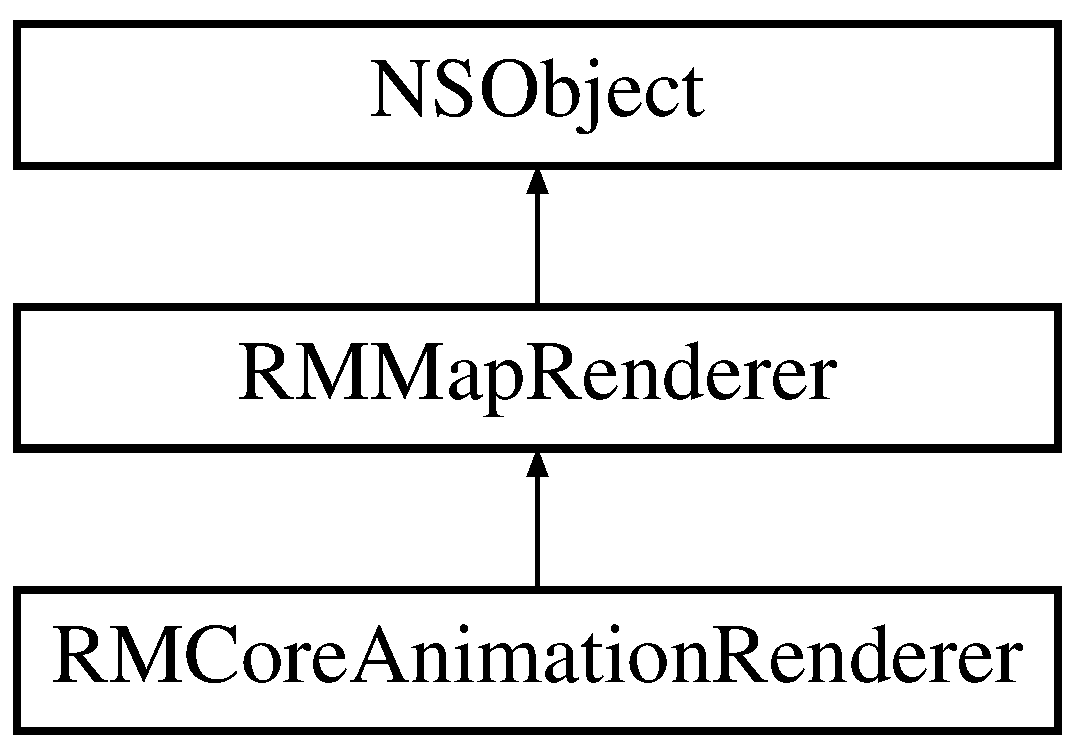
\includegraphics[height=3.000000cm]{interface_r_m_map_renderer}
\end{center}
\end{figure}
\subsection*{Instance Methods}
\begin{DoxyCompactItemize}
\item 
(void) -\/ \hyperlink{interface_r_m_map_renderer_a171d7fd81412009ed1f92f27c5ec6f2a}{dealloc}{\ttfamily  \mbox{[}implementation\mbox{]}}
\item 
(void) -\/ \hyperlink{interface_r_m_map_renderer_a0f3802416a587d84d9b04b289f577190}{draw\-Rect\-:}
\item 
(id) -\/ \hyperlink{interface_r_m_map_renderer_a439495e611ee8960c35d5272089f7b57}{init\-With\-Content\-:}
\item 
(C\-A\-Layer $\ast$) -\/ \hyperlink{interface_r_m_map_renderer_a388de8a3bd1c56a07bc69f8967f34037}{layer}
\item 
(void) -\/ \hyperlink{interface_r_m_map_renderer_aa509a04f8b9702d4a4ea3010ca681f05}{map\-Image\-Loaded\-:}{\ttfamily  \mbox{[}implementation\mbox{]}}
\item 
(void) -\/ \hyperlink{interface_r_m_map_renderer_a9191dc45f6215897f0e601e085850d1d}{set\-Frame\-:}
\item 
(void) -\/ \hyperlink{interface_r_m_map_renderer_a5351f5a213da59e4646c0ad6e49db22b}{set\-Needs\-Display}
\end{DoxyCompactItemize}
\subsection*{Protected 属性}
\begin{DoxyCompactItemize}
\item 
\hyperlink{interface_r_m_map_contents}{R\-M\-Map\-Contents} $\ast$ \hyperlink{interface_r_m_map_renderer_a6dc63e478a69b3262bd89acb37ea7bcb}{content}
\end{DoxyCompactItemize}


\subsection{Method Documentation}
\hypertarget{interface_r_m_map_renderer_a171d7fd81412009ed1f92f27c5ec6f2a}{\index{R\-M\-Map\-Renderer@{R\-M\-Map\-Renderer}!dealloc@{dealloc}}
\index{dealloc@{dealloc}!RMMapRenderer@{R\-M\-Map\-Renderer}}
\subsubsection[{dealloc}]{\setlength{\rightskip}{0pt plus 5cm}-\/ (void) dealloc 
\begin{DoxyParamCaption}
{}
\end{DoxyParamCaption}
\hspace{0.3cm}{\ttfamily [implementation]}}}\label{interface_r_m_map_renderer_a171d7fd81412009ed1f92f27c5ec6f2a}


被 \hyperlink{interface_r_m_core_animation_renderer_a042e89d2923653a122204ce1fa2efa70}{R\-M\-Core\-Animation\-Renderer} 重载.



参考自 R\-M\-Core\-Animation\-Renderer\-::dealloc.

\hypertarget{interface_r_m_map_renderer_a0f3802416a587d84d9b04b289f577190}{\index{R\-M\-Map\-Renderer@{R\-M\-Map\-Renderer}!draw\-Rect\-:@{draw\-Rect\-:}}
\index{draw\-Rect\-:@{draw\-Rect\-:}!RMMapRenderer@{R\-M\-Map\-Renderer}}
\subsubsection[{draw\-Rect\-:}]{\setlength{\rightskip}{0pt plus 5cm}-\/ (void) draw\-Rect\-: 
\begin{DoxyParamCaption}
\item[{(C\-G\-Rect)}]{rect}
\end{DoxyParamCaption}
}}\label{interface_r_m_map_renderer_a0f3802416a587d84d9b04b289f577190}
\begin{DoxyRefDesc}{Bug}
\item[\hyperlink{bug__bug000021}{Bug}]no-\/op \end{DoxyRefDesc}


参考自 R\-M\-Map\-Contents\-::draw\-Rect\-:.

\hypertarget{interface_r_m_map_renderer_a439495e611ee8960c35d5272089f7b57}{\index{R\-M\-Map\-Renderer@{R\-M\-Map\-Renderer}!init\-With\-Content\-:@{init\-With\-Content\-:}}
\index{init\-With\-Content\-:@{init\-With\-Content\-:}!RMMapRenderer@{R\-M\-Map\-Renderer}}
\subsubsection[{init\-With\-Content\-:}]{\setlength{\rightskip}{0pt plus 5cm}-\/ (id) init\-With\-Content\-: 
\begin{DoxyParamCaption}
\item[{({\bf R\-M\-Map\-Contents} $\ast$)}]{contents}
\end{DoxyParamCaption}
}}\label{interface_r_m_map_renderer_a439495e611ee8960c35d5272089f7b57}


被 \hyperlink{interface_r_m_core_animation_renderer_a0a684a7d8ba7065b4223b3079d8c3483}{R\-M\-Core\-Animation\-Renderer} 重载.

\hypertarget{interface_r_m_map_renderer_a388de8a3bd1c56a07bc69f8967f34037}{\index{R\-M\-Map\-Renderer@{R\-M\-Map\-Renderer}!layer@{layer}}
\index{layer@{layer}!RMMapRenderer@{R\-M\-Map\-Renderer}}
\subsubsection[{layer}]{\setlength{\rightskip}{0pt plus 5cm}-\/ (C\-A\-Layer $\ast$) layer 
\begin{DoxyParamCaption}
{}
\end{DoxyParamCaption}
}}\label{interface_r_m_map_renderer_a388de8a3bd1c56a07bc69f8967f34037}
\begin{DoxyRefDesc}{Bug}
\item[\hyperlink{bug__bug000023}{Bug}]no-\/op \end{DoxyRefDesc}


被 \hyperlink{interface_r_m_core_animation_renderer_ab37d6e7a835c2d88bc51bd4a21d5f5ca}{R\-M\-Core\-Animation\-Renderer} 重载.



参考自 R\-M\-Map\-Contents\-::set\-Background\-:, R\-M\-Map\-Contents\-::set\-Overlay\-: , 以及 R\-M\-Map\-Contents\-::set\-Renderer\-:.

\hypertarget{interface_r_m_map_renderer_aa509a04f8b9702d4a4ea3010ca681f05}{\index{R\-M\-Map\-Renderer@{R\-M\-Map\-Renderer}!map\-Image\-Loaded\-:@{map\-Image\-Loaded\-:}}
\index{map\-Image\-Loaded\-:@{map\-Image\-Loaded\-:}!RMMapRenderer@{R\-M\-Map\-Renderer}}
\subsubsection[{map\-Image\-Loaded\-:}]{\setlength{\rightskip}{0pt plus 5cm}-\/ (void) map\-Image\-Loaded\-: 
\begin{DoxyParamCaption}
\item[{(N\-S\-Notification$\ast$)}]{notification}
\end{DoxyParamCaption}
\hspace{0.3cm}{\ttfamily [implementation]}}}\label{interface_r_m_map_renderer_aa509a04f8b9702d4a4ea3010ca681f05}
\begin{DoxyRefDesc}{Bug}
\item[\hyperlink{bug__bug000020}{Bug}]calls a no-\/op \end{DoxyRefDesc}


被 \hyperlink{interface_r_m_core_animation_renderer_a0bf0f1d99f3d6b98583ae637139e245a}{R\-M\-Core\-Animation\-Renderer} 重载.

\hypertarget{interface_r_m_map_renderer_a9191dc45f6215897f0e601e085850d1d}{\index{R\-M\-Map\-Renderer@{R\-M\-Map\-Renderer}!set\-Frame\-:@{set\-Frame\-:}}
\index{set\-Frame\-:@{set\-Frame\-:}!RMMapRenderer@{R\-M\-Map\-Renderer}}
\subsubsection[{set\-Frame\-:}]{\setlength{\rightskip}{0pt plus 5cm}-\/ (void) set\-Frame\-: 
\begin{DoxyParamCaption}
\item[{(C\-G\-Rect)}]{frame}
\end{DoxyParamCaption}
}}\label{interface_r_m_map_renderer_a9191dc45f6215897f0e601e085850d1d}
\begin{DoxyRefDesc}{Bug}
\item[\hyperlink{bug__bug000022}{Bug}]no-\/op \end{DoxyRefDesc}


被 \hyperlink{interface_r_m_core_animation_renderer_ad46d40355e2c34bcf66663d802118035}{R\-M\-Core\-Animation\-Renderer} 重载.



参考自 R\-M\-Map\-Contents\-::set\-Frame\-:.

\hypertarget{interface_r_m_map_renderer_a5351f5a213da59e4646c0ad6e49db22b}{\index{R\-M\-Map\-Renderer@{R\-M\-Map\-Renderer}!set\-Needs\-Display@{set\-Needs\-Display}}
\index{set\-Needs\-Display@{set\-Needs\-Display}!RMMapRenderer@{R\-M\-Map\-Renderer}}
\subsubsection[{set\-Needs\-Display}]{\setlength{\rightskip}{0pt plus 5cm}-\/ (void) set\-Needs\-Display 
\begin{DoxyParamCaption}
{}
\end{DoxyParamCaption}
}}\label{interface_r_m_map_renderer_a5351f5a213da59e4646c0ad6e49db22b}
\begin{DoxyRefDesc}{Bug}
\item[\hyperlink{bug__bug000019}{Bug}]no-\/op \end{DoxyRefDesc}


参考自 map\-Image\-Loaded\-:, R\-M\-Map\-Contents\-::move\-By\-:, R\-M\-Map\-Contents\-::set\-Center\-Projected\-Point\-:, R\-M\-Map\-Contents\-::set\-Meters\-Per\-Pixel\-:, R\-M\-Map\-Contents\-::zoom\-By\-Factor\-:near\-:, R\-M\-Map\-Contents\-::zoom\-By\-Factor\-:near\-:animated\-:with\-Callback\-: , 以及 R\-M\-Map\-Contents\-::zoom\-With\-R\-M\-Mercator\-Rect\-Bounds\-:.



\subsection{类成员变量说明}
\hypertarget{interface_r_m_map_renderer_a6dc63e478a69b3262bd89acb37ea7bcb}{\index{R\-M\-Map\-Renderer@{R\-M\-Map\-Renderer}!content@{content}}
\index{content@{content}!RMMapRenderer@{R\-M\-Map\-Renderer}}
\subsubsection[{content}]{\setlength{\rightskip}{0pt plus 5cm}-\/ ({\bf R\-M\-Map\-Contents}$\ast$) content\hspace{0.3cm}{\ttfamily [protected]}}}\label{interface_r_m_map_renderer_a6dc63e478a69b3262bd89acb37ea7bcb}


参考自 R\-M\-Core\-Animation\-Renderer\-::init\-With\-Content\-:, init\-With\-Content\-: , 以及 R\-M\-Core\-Animation\-Renderer\-::set\-Frame\-:.



该类的文档由以下文件生成\-:\begin{DoxyCompactItemize}
\item 
Map/\hyperlink{_r_m_map_renderer_8h}{R\-M\-Map\-Renderer.\-h}\item 
Map/\hyperlink{_r_m_map_renderer_8m}{R\-M\-Map\-Renderer.\-m}\end{DoxyCompactItemize}

\hypertarget{interface_r_m_map_view}{\section{R\-M\-Map\-View类 参考}
\label{interface_r_m_map_view}\index{R\-M\-Map\-View@{R\-M\-Map\-View}}
}


Wrapper around \hyperlink{interface_r_m_map_contents}{R\-M\-Map\-Contents} for the i\-Phone.  




{\ttfamily \#import $<$R\-M\-Map\-View.\-h$>$}

类 R\-M\-Map\-View 继承关系图\-:\begin{figure}[H]
\begin{center}
\leavevmode
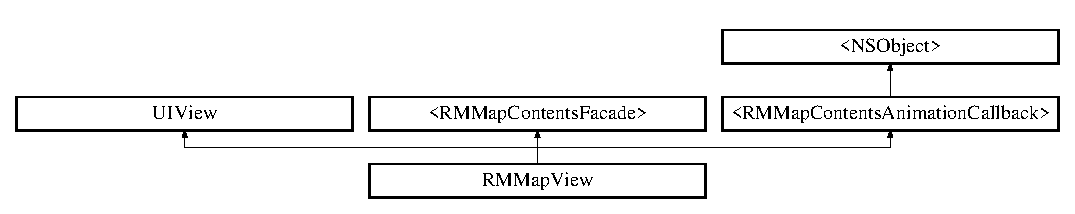
\includegraphics[height=2.424242cm]{interface_r_m_map_view}
\end{center}
\end{figure}
\subsection*{Instance Methods}
\begin{DoxyCompactItemize}
\item 
(void) -\/ \hyperlink{interface_r_m_map_view_ab512cbaf772a0c0b6a8a8fb10f80d2b4}{animation\-Finished\-With\-Zoom\-Factor\-:near\-:}{\ttfamily  \mbox{[}implementation\mbox{]}}
\item 
(void) -\/ \hyperlink{interface_r_m_map_view_a795716de54229787251beb8957477905}{animation\-Stepped}{\ttfamily  \mbox{[}implementation\mbox{]}}
\item 
(B\-O\-O\-L) -\/ \hyperlink{interface_r_m_map_view_a71183d1cfbc01ab7fa3c60890165e195}{can\-Become\-First\-Responder}{\ttfamily  \mbox{[}implementation\mbox{]}}
\item 
(void) -\/ \hyperlink{interface_r_m_map_view_a617a8a88530a946d5eb3a1f759286e8b}{dealloc}{\ttfamily  \mbox{[}implementation\mbox{]}}
\item 
(void) -\/ \hyperlink{interface_r_m_map_view_a3c77bbe947d54f2204c507964958d00c}{delayed\-Resume\-Expensive\-Operations}{\ttfamily  \mbox{[}implementation\mbox{]}}
\item 
(N\-S\-String $\ast$) -\/ \hyperlink{interface_r_m_map_view_aa23a642a33fd21939aee40ba44e20a6f}{description}{\ttfamily  \mbox{[}implementation\mbox{]}}
\item 
(void) -\/ \hyperlink{interface_r_m_map_view_ae58c168c733c803c56654428f0c8f3f8}{did\-Receive\-Memory\-Warning}
\begin{DoxyCompactList}\small\item\em Must be called by higher did\-Receive\-Memory\-Warning. \end{DoxyCompactList}\item 
(void) -\/ \hyperlink{interface_r_m_map_view_a7f702df1576c7b8db4b2173c6902700c}{draw\-Rect\-:}{\ttfamily  \mbox{[}implementation\mbox{]}}
\item 
(void) -\/ \hyperlink{interface_r_m_map_view_af7d6b307e05ec8764af12246115b96f8}{forward\-Invocation\-:}{\ttfamily  \mbox{[}implementation\mbox{]}}
\begin{DoxyCompactList}\small\item\em Forward invocations to \hyperlink{interface_r_m_map_contents}{R\-M\-Map\-Contents}. \end{DoxyCompactList}\item 
(\hyperlink{struct_r_m_gesture_details}{R\-M\-Gesture\-Details}) -\/ \hyperlink{interface_r_m_map_view_abb2649a394b8b7289abeec07085fcf57}{gesture\-Details\-:}{\ttfamily  \mbox{[}implementation\mbox{]}}
\item 
(void) -\/ \hyperlink{interface_r_m_map_view_a1437dbaa8dbeb7dd1c39e64af6fe67e9}{increment\-Deceleration\-:}{\ttfamily  \mbox{[}implementation\mbox{]}}
\item 
(id) -\/ \hyperlink{interface_r_m_map_view_a71b21d934e08438432276751ae143724}{init\-With\-Frame\-:}
\item 
(id) -\/ \hyperlink{interface_r_m_map_view_a0f9e140d1265f696965fa73730fdf7e3}{init\-With\-Frame\-:screen\-Scale\-:}
\item 
(id) -\/ \hyperlink{interface_r_m_map_view_adcd80394c57cbe77208bfc6726ff94dd}{init\-With\-Frame\-:\-With\-Location\-:}
\item 
(N\-S\-Method\-Signature $\ast$) -\/ \hyperlink{interface_r_m_map_view_ab97fa7e84b093b0e309ffe18cec6ffad}{method\-Signature\-For\-Selector\-:}{\ttfamily  \mbox{[}implementation\mbox{]}}
\item 
(void) -\/ \hyperlink{interface_r_m_map_view_a27baf3f4a31aca87ce9f1a54437b1af0}{move\-By\-:}
\item 
(void) -\/ \hyperlink{interface_r_m_map_view_a1097238683168693264f3f1fd0e69f80}{move\-To\-Lat\-Long\-:}
\begin{DoxyCompactList}\small\item\em recenter the map on \#latlong, expressed as C\-L\-Location\-Coordinate2\-D (latitude/longitude) \end{DoxyCompactList}\item 
(void) -\/ \hyperlink{interface_r_m_map_view_a7a576fb939de0ccc3e50f5f92ef9718d}{move\-To\-Projected\-Point\-:}
\begin{DoxyCompactList}\small\item\em recenter the map on \#a\-Point, expressed in projected meters \end{DoxyCompactList}\item 
(void) -\/ \hyperlink{interface_r_m_map_view_a8eef4d40f5482cf90fe43a8e98f5dba8}{perform\-Initial\-Setup}{\ttfamily  \mbox{[}implementation\mbox{]}}
\item 
(void) -\/ \hyperlink{interface_r_m_map_view_acb8af34cf5b0de81f4643bdcb19c0a59}{resume\-Expensive\-Operations}{\ttfamily  \mbox{[}implementation\mbox{]}}
\item 
(void) -\/ \hyperlink{interface_r_m_map_view_ac72f6a4091d84d904b65b303fac6bd25}{set\-Constraints\-S\-W\-:\-N\-E\-:}
\item 
(void) -\/ \hyperlink{interface_r_m_map_view_a489d7ac50d1ac7c2629db80141e7f8a6}{set\-Contents\-:}{\ttfamily  \mbox{[}implementation\mbox{]}}
\item 
(void) -\/ \hyperlink{interface_r_m_map_view_aea8bf2b4af3776170dc88d64d18c83bf}{set\-Delegate\-:}{\ttfamily  \mbox{[}implementation\mbox{]}}
\item 
(void) -\/ \hyperlink{interface_r_m_map_view_ab6e0beac983f26b40a756dda0498710e}{set\-Frame\-:}{\ttfamily  \mbox{[}implementation\mbox{]}}
\item 
(void) -\/ \hyperlink{interface_r_m_map_view_ae1cfbd98780426dfee0d008fc51651ea}{set\-Projected\-Contraints\-S\-W\-:\-N\-E\-:}
\item 
(void) -\/ \hyperlink{interface_r_m_map_view_a7532fc82b570c3e7f81d559717acec6e}{set\-Rotation\-:}
\item 
(void) -\/ \hyperlink{interface_r_m_map_view_a0634cae1a974936b4dde86e0392a6c33}{start\-Deceleration\-With\-Delta\-:}{\ttfamily  \mbox{[}implementation\mbox{]}}
\item 
(void) -\/ \hyperlink{interface_r_m_map_view_a85d36e113ba408b7beeb23a7354156c2}{stop\-Deceleration}{\ttfamily  \mbox{[}implementation\mbox{]}}
\item 
(void) -\/ \hyperlink{interface_r_m_map_view_ae441d7ab885d8dd18b794a68c113e4cb}{touches\-Began\-:with\-Event\-:}{\ttfamily  \mbox{[}implementation\mbox{]}}
\item 
(void) -\/ \hyperlink{interface_r_m_map_view_a464f5e8b6bdf7ce72e7e30e17972a047}{touches\-Cancelled\-:with\-Event\-:}{\ttfamily  \mbox{[}implementation\mbox{]}}
\item 
(void) -\/ \hyperlink{interface_r_m_map_view_a064931bc77db98015373c5d76faf9226}{touches\-Ended\-:with\-Event\-:}{\ttfamily  \mbox{[}implementation\mbox{]}}
\item 
(void) -\/ \hyperlink{interface_r_m_map_view_ace3bf92bf491646d749c27f55d2d7b34}{touches\-Moved\-:with\-Event\-:}{\ttfamily  \mbox{[}implementation\mbox{]}}
\item 
(void) -\/ \hyperlink{interface_r_m_map_view_a6003bcb4479e3ca7f2500db18f7ee8e8}{zoom\-By\-Factor\-:near\-:}
\item 
(void) -\/ \hyperlink{interface_r_m_map_view_a30bd6e4766b3bc224a6e214bb06ec8ca}{zoom\-By\-Factor\-:near\-:animated\-:}
\end{DoxyCompactItemize}
\subsection*{Protected 属性}
\begin{DoxyCompactItemize}
\item 
\hyperlink{struct_r_m_gesture_details}{R\-M\-Gesture\-Details} \hyperlink{interface_r_m_map_view_a9b8031da19d9d7850a4795cbbadefa5c}{last\-Gesture}
\item 
\hyperlink{interface_r_m_s_m_layer_info}{R\-M\-S\-M\-Layer\-Info} $\ast$ \hyperlink{interface_r_m_map_view_aca406dc0027962e811a73ee69ce5db68}{m\-\_\-info}
\item 
\hyperlink{interface_r_m_s_m_tile_source}{R\-M\-S\-M\-Tile\-Source} $\ast$ \hyperlink{interface_r_m_map_view_af89039ac8817690a1dceadd43b44ab8f}{m\-\_\-\-Tile\-Source}
\item 
float \hyperlink{interface_r_m_map_view_a51d17c6a26beb3cbd1bf51de4aa1f774}{screen\-Scale}
\end{DoxyCompactItemize}
\subsection*{属性}
\begin{DoxyCompactItemize}
\item 
\hyperlink{interface_r_m_map_contents}{R\-M\-Map\-Contents} $\ast$ \hyperlink{interface_r_m_map_view_a87dc341bead16abfa5b0f23260ac6ed9}{contents}
\begin{DoxyCompactList}\small\item\em Any other functionality you need to manipulate the map you can access through this property. \end{DoxyCompactList}\item 
B\-O\-O\-L \hyperlink{interface_r_m_map_view_aba614ce906ab6f54581593002a4a6e78}{deceleration}
\item 
float \hyperlink{interface_r_m_map_view_a1e9a66251764c79b4b6c43dc92d8d245}{deceleration\-Factor}
\item 
id$<$ \hyperlink{protocol_r_m_map_view_delegate-p}{R\-M\-Map\-View\-Delegate} $>$ \hyperlink{interface_r_m_map_view_a4703ad41a6e6ace59dc9e1bee3d3f382}{delegate}
\item 
B\-O\-O\-L \hyperlink{interface_r_m_map_view_a3ce66092f0dcae73e0d209c9dab6c580}{enable\-Dragging}
\item 
B\-O\-O\-L \hyperlink{interface_r_m_map_view_a0be5c05b118052c1c802a4afda276d6c}{enable\-Rotate}
\item 
B\-O\-O\-L \hyperlink{interface_r_m_map_view_a317f8fffb2cd671dd1c8b4fb90d4b7fa}{enable\-Zoom}
\item 
\hyperlink{interface_r_m_marker_manager}{R\-M\-Marker\-Manager} $\ast$ \hyperlink{interface_r_m_map_view_adb35b8ebc9e8cddb3bfdf560c2d921dd}{marker\-Manager}
\item 
C\-G\-Float \hyperlink{interface_r_m_map_view_a5db051adefc02909422ab8452b0db6f2}{rotation}
\end{DoxyCompactItemize}


\subsection{详细描述}
Wrapper around \hyperlink{interface_r_m_map_contents}{R\-M\-Map\-Contents} for the i\-Phone. 

It implements event handling; but that's about it. All the interesting map logic is done by \hyperlink{interface_r_m_map_contents}{R\-M\-Map\-Contents}. There is exactly one \hyperlink{interface_r_m_map_view}{R\-M\-Map\-View} instance for each \hyperlink{interface_r_m_map_contents}{R\-M\-Map\-Contents} instance.

A -\/forward\-Invocation method exists for R\-M\-Map, and forwards all unhandled messages to the \hyperlink{interface_r_m_map_contents}{R\-M\-Map\-Contents} instance.

\begin{DoxyRefDesc}{Bug}
\item[\hyperlink{bug__bug000024}{Bug}]No accessors for enable\-Dragging, enable\-Zoom, deceleration, deceleration\-Factor. Changing enable\-Dragging does not change multitouch\-Enabled for the view. \end{DoxyRefDesc}


\subsection{Method Documentation}
\hypertarget{interface_r_m_map_view_ab512cbaf772a0c0b6a8a8fb10f80d2b4}{\index{R\-M\-Map\-View@{R\-M\-Map\-View}!animation\-Finished\-With\-Zoom\-Factor\-:near\-:@{animation\-Finished\-With\-Zoom\-Factor\-:near\-:}}
\index{animation\-Finished\-With\-Zoom\-Factor\-:near\-:@{animation\-Finished\-With\-Zoom\-Factor\-:near\-:}!RMMapView@{R\-M\-Map\-View}}
\subsubsection[{animation\-Finished\-With\-Zoom\-Factor\-:near\-:}]{\setlength{\rightskip}{0pt plus 5cm}-\/ (void) animation\-Finished\-With\-Zoom\-Factor\-: 
\begin{DoxyParamCaption}
\item[{(float)}]{zoom\-Factor}
\item[{near:(C\-G\-Point)}]{p}
\end{DoxyParamCaption}
\hspace{0.3cm}{\ttfamily [implementation]}}}\label{interface_r_m_map_view_ab512cbaf772a0c0b6a8a8fb10f80d2b4}


重载 \hyperlink{protocol_r_m_map_contents_animation_callback-p_afd3a55e53810bb11b843754ffa4d346d}{$<$\-R\-M\-Map\-Contents\-Animation\-Callback$>$} .

\hypertarget{interface_r_m_map_view_a795716de54229787251beb8957477905}{\index{R\-M\-Map\-View@{R\-M\-Map\-View}!animation\-Stepped@{animation\-Stepped}}
\index{animation\-Stepped@{animation\-Stepped}!RMMapView@{R\-M\-Map\-View}}
\subsubsection[{animation\-Stepped}]{\setlength{\rightskip}{0pt plus 5cm}-\/ (void) animation\-Stepped 
\begin{DoxyParamCaption}
{}
\end{DoxyParamCaption}
\hspace{0.3cm}{\ttfamily [implementation]}}}\label{interface_r_m_map_view_a795716de54229787251beb8957477905}


重载 \hyperlink{protocol_r_m_map_contents_animation_callback-p_a404de1d6b9991d9daf716996b515ec6c}{$<$\-R\-M\-Map\-Contents\-Animation\-Callback$>$} .

\hypertarget{interface_r_m_map_view_a71183d1cfbc01ab7fa3c60890165e195}{\index{R\-M\-Map\-View@{R\-M\-Map\-View}!can\-Become\-First\-Responder@{can\-Become\-First\-Responder}}
\index{can\-Become\-First\-Responder@{can\-Become\-First\-Responder}!RMMapView@{R\-M\-Map\-View}}
\subsubsection[{can\-Become\-First\-Responder}]{\setlength{\rightskip}{0pt plus 5cm}-\/ (B\-O\-O\-L) can\-Become\-First\-Responder 
\begin{DoxyParamCaption}
{}
\end{DoxyParamCaption}
\hspace{0.3cm}{\ttfamily [implementation]}}}\label{interface_r_m_map_view_a71183d1cfbc01ab7fa3c60890165e195}
\hypertarget{interface_r_m_map_view_a617a8a88530a946d5eb3a1f759286e8b}{\index{R\-M\-Map\-View@{R\-M\-Map\-View}!dealloc@{dealloc}}
\index{dealloc@{dealloc}!RMMapView@{R\-M\-Map\-View}}
\subsubsection[{dealloc}]{\setlength{\rightskip}{0pt plus 5cm}-\/ (void) dealloc 
\begin{DoxyParamCaption}
{}
\end{DoxyParamCaption}
\hspace{0.3cm}{\ttfamily [implementation]}}}\label{interface_r_m_map_view_a617a8a88530a946d5eb3a1f759286e8b}
\hypertarget{interface_r_m_map_view_a3c77bbe947d54f2204c507964958d00c}{\index{R\-M\-Map\-View@{R\-M\-Map\-View}!delayed\-Resume\-Expensive\-Operations@{delayed\-Resume\-Expensive\-Operations}}
\index{delayed\-Resume\-Expensive\-Operations@{delayed\-Resume\-Expensive\-Operations}!RMMapView@{R\-M\-Map\-View}}
\subsubsection[{delayed\-Resume\-Expensive\-Operations}]{\setlength{\rightskip}{0pt plus 5cm}-\/ (void) delayed\-Resume\-Expensive\-Operations 
\begin{DoxyParamCaption}
{}
\end{DoxyParamCaption}
\hspace{0.3cm}{\ttfamily [implementation]}}}\label{interface_r_m_map_view_a3c77bbe947d54f2204c507964958d00c}


参考自 increment\-Deceleration\-:, touches\-Began\-:with\-Event\-:, touches\-Cancelled\-:with\-Event\-:, touches\-Ended\-:with\-Event\-: , 以及 touches\-Moved\-:with\-Event\-:.

\hypertarget{interface_r_m_map_view_aa23a642a33fd21939aee40ba44e20a6f}{\index{R\-M\-Map\-View@{R\-M\-Map\-View}!description@{description}}
\index{description@{description}!RMMapView@{R\-M\-Map\-View}}
\subsubsection[{description}]{\setlength{\rightskip}{0pt plus 5cm}-\/ (N\-S\-String $\ast$) description 
\begin{DoxyParamCaption}
{}
\end{DoxyParamCaption}
\hspace{0.3cm}{\ttfamily [implementation]}}}\label{interface_r_m_map_view_aa23a642a33fd21939aee40ba44e20a6f}
\hypertarget{interface_r_m_map_view_ae58c168c733c803c56654428f0c8f3f8}{\index{R\-M\-Map\-View@{R\-M\-Map\-View}!did\-Receive\-Memory\-Warning@{did\-Receive\-Memory\-Warning}}
\index{did\-Receive\-Memory\-Warning@{did\-Receive\-Memory\-Warning}!RMMapView@{R\-M\-Map\-View}}
\subsubsection[{did\-Receive\-Memory\-Warning}]{\setlength{\rightskip}{0pt plus 5cm}-\/ (void) did\-Receive\-Memory\-Warning 
\begin{DoxyParamCaption}
{}
\end{DoxyParamCaption}
}}\label{interface_r_m_map_view_ae58c168c733c803c56654428f0c8f3f8}


Must be called by higher did\-Receive\-Memory\-Warning. 

\hypertarget{interface_r_m_map_view_a7f702df1576c7b8db4b2173c6902700c}{\index{R\-M\-Map\-View@{R\-M\-Map\-View}!draw\-Rect\-:@{draw\-Rect\-:}}
\index{draw\-Rect\-:@{draw\-Rect\-:}!RMMapView@{R\-M\-Map\-View}}
\subsubsection[{draw\-Rect\-:}]{\setlength{\rightskip}{0pt plus 5cm}-\/ (void) draw\-Rect\-: 
\begin{DoxyParamCaption}
\item[{(C\-G\-Rect)}]{rect}
\end{DoxyParamCaption}
\hspace{0.3cm}{\ttfamily [implementation]}}}\label{interface_r_m_map_view_a7f702df1576c7b8db4b2173c6902700c}


参考自 draw\-Rect\-:.

\hypertarget{interface_r_m_map_view_af7d6b307e05ec8764af12246115b96f8}{\index{R\-M\-Map\-View@{R\-M\-Map\-View}!forward\-Invocation\-:@{forward\-Invocation\-:}}
\index{forward\-Invocation\-:@{forward\-Invocation\-:}!RMMapView@{R\-M\-Map\-View}}
\subsubsection[{forward\-Invocation\-:}]{\setlength{\rightskip}{0pt plus 5cm}-\/ (void) forward\-Invocation\-: 
\begin{DoxyParamCaption}
\item[{(N\-S\-Invocation $\ast$)}]{invocation}
\end{DoxyParamCaption}
\hspace{0.3cm}{\ttfamily [implementation]}}}\label{interface_r_m_map_view_af7d6b307e05ec8764af12246115b96f8}


Forward invocations to \hyperlink{interface_r_m_map_contents}{R\-M\-Map\-Contents}. 

\hypertarget{interface_r_m_map_view_abb2649a394b8b7289abeec07085fcf57}{\index{R\-M\-Map\-View@{R\-M\-Map\-View}!gesture\-Details\-:@{gesture\-Details\-:}}
\index{gesture\-Details\-:@{gesture\-Details\-:}!RMMapView@{R\-M\-Map\-View}}
\subsubsection[{gesture\-Details\-:}]{\setlength{\rightskip}{0pt plus 5cm}-\/ ({\bf R\-M\-Gesture\-Details}) gesture\-Details\-: 
\begin{DoxyParamCaption}
\item[{(N\-S\-Set$\ast$)}]{touches}
\end{DoxyParamCaption}
\hspace{0.3cm}{\ttfamily [implementation]}}}\label{interface_r_m_map_view_abb2649a394b8b7289abeec07085fcf57}


参考自 touches\-Began\-:with\-Event\-:, touches\-Ended\-:with\-Event\-: , 以及 touches\-Moved\-:with\-Event\-:.

\hypertarget{interface_r_m_map_view_a1437dbaa8dbeb7dd1c39e64af6fe67e9}{\index{R\-M\-Map\-View@{R\-M\-Map\-View}!increment\-Deceleration\-:@{increment\-Deceleration\-:}}
\index{increment\-Deceleration\-:@{increment\-Deceleration\-:}!RMMapView@{R\-M\-Map\-View}}
\subsubsection[{increment\-Deceleration\-:}]{\setlength{\rightskip}{0pt plus 5cm}-\/ (void) increment\-Deceleration\-: 
\begin{DoxyParamCaption}
\item[{(N\-S\-Timer $\ast$)}]{timer}
\end{DoxyParamCaption}
\hspace{0.3cm}{\ttfamily [implementation]}}}\label{interface_r_m_map_view_a1437dbaa8dbeb7dd1c39e64af6fe67e9}


Provided by category \hyperlink{category_r_m_map_view_07_private_methods_08_ad33d83d9abe096685ce0c34fd71ca94f}{R\-M\-Map\-View(\-Private\-Methods)}.

\hypertarget{interface_r_m_map_view_a71b21d934e08438432276751ae143724}{\index{R\-M\-Map\-View@{R\-M\-Map\-View}!init\-With\-Frame\-:@{init\-With\-Frame\-:}}
\index{init\-With\-Frame\-:@{init\-With\-Frame\-:}!RMMapView@{R\-M\-Map\-View}}
\subsubsection[{init\-With\-Frame\-:}]{\setlength{\rightskip}{0pt plus 5cm}-\/ (id) init\-With\-Frame\-: 
\begin{DoxyParamCaption}
\item[{(C\-G\-Rect)}]{frame}
\end{DoxyParamCaption}
}}\label{interface_r_m_map_view_a71b21d934e08438432276751ae143724}
\hypertarget{interface_r_m_map_view_a0f9e140d1265f696965fa73730fdf7e3}{\index{R\-M\-Map\-View@{R\-M\-Map\-View}!init\-With\-Frame\-:screen\-Scale\-:@{init\-With\-Frame\-:screen\-Scale\-:}}
\index{init\-With\-Frame\-:screen\-Scale\-:@{init\-With\-Frame\-:screen\-Scale\-:}!RMMapView@{R\-M\-Map\-View}}
\subsubsection[{init\-With\-Frame\-:screen\-Scale\-:}]{\setlength{\rightskip}{0pt plus 5cm}-\/ (id) {\bf init\-With\-Frame\-:} 
\begin{DoxyParamCaption}
\item[{(C\-G\-Rect)}]{frame}
\item[{screenScale:(float)}]{screen\-Scale}
\end{DoxyParamCaption}
}}\label{interface_r_m_map_view_a0f9e140d1265f696965fa73730fdf7e3}


参考自 init\-With\-Frame\-:.

\hypertarget{interface_r_m_map_view_adcd80394c57cbe77208bfc6726ff94dd}{\index{R\-M\-Map\-View@{R\-M\-Map\-View}!init\-With\-Frame\-:\-With\-Location\-:@{init\-With\-Frame\-:\-With\-Location\-:}}
\index{init\-With\-Frame\-:\-With\-Location\-:@{init\-With\-Frame\-:\-With\-Location\-:}!RMMapView@{R\-M\-Map\-View}}
\subsubsection[{init\-With\-Frame\-:\-With\-Location\-:}]{\setlength{\rightskip}{0pt plus 5cm}-\/ (id) {\bf init\-With\-Frame\-:} 
\begin{DoxyParamCaption}
\item[{(C\-G\-Rect)}]{frame}
\item[{WithLocation:(C\-L\-Location\-Coordinate2\-D)}]{latlon}
\end{DoxyParamCaption}
}}\label{interface_r_m_map_view_adcd80394c57cbe77208bfc6726ff94dd}
\begin{DoxyRefDesc}{弃用}
\item[\hyperlink{deprecated__deprecated000010}{弃用}]Deprecated any time after 0.\-5. \end{DoxyRefDesc}
\hypertarget{interface_r_m_map_view_ab97fa7e84b093b0e309ffe18cec6ffad}{\index{R\-M\-Map\-View@{R\-M\-Map\-View}!method\-Signature\-For\-Selector\-:@{method\-Signature\-For\-Selector\-:}}
\index{method\-Signature\-For\-Selector\-:@{method\-Signature\-For\-Selector\-:}!RMMapView@{R\-M\-Map\-View}}
\subsubsection[{method\-Signature\-For\-Selector\-:}]{\setlength{\rightskip}{0pt plus 5cm}-\/ (N\-S\-Method\-Signature $\ast$) method\-Signature\-For\-Selector\-: 
\begin{DoxyParamCaption}
\item[{(S\-E\-L)}]{a\-Selector}
\end{DoxyParamCaption}
\hspace{0.3cm}{\ttfamily [implementation]}}}\label{interface_r_m_map_view_ab97fa7e84b093b0e309ffe18cec6ffad}


参考自 method\-Signature\-For\-Selector\-:.

\hypertarget{interface_r_m_map_view_a27baf3f4a31aca87ce9f1a54437b1af0}{\index{R\-M\-Map\-View@{R\-M\-Map\-View}!move\-By\-:@{move\-By\-:}}
\index{move\-By\-:@{move\-By\-:}!RMMapView@{R\-M\-Map\-View}}
\subsubsection[{move\-By\-:}]{\setlength{\rightskip}{0pt plus 5cm}-\/ (void) move\-By\-: 
\begin{DoxyParamCaption}
\item[{(C\-G\-Size)}]{delta}
\end{DoxyParamCaption}
}}\label{interface_r_m_map_view_a27baf3f4a31aca87ce9f1a54437b1af0}


重载 \hyperlink{protocol_r_m_map_contents_facade-p_a229f6bcfb540a9afb2f1620c2e79fcb2}{$<$\-R\-M\-Map\-Contents\-Facade$>$} .



参考自 increment\-Deceleration\-:, move\-By\-:, stop\-Deceleration , 以及 touches\-Moved\-:with\-Event\-:.

\hypertarget{interface_r_m_map_view_a1097238683168693264f3f1fd0e69f80}{\index{R\-M\-Map\-View@{R\-M\-Map\-View}!move\-To\-Lat\-Long\-:@{move\-To\-Lat\-Long\-:}}
\index{move\-To\-Lat\-Long\-:@{move\-To\-Lat\-Long\-:}!RMMapView@{R\-M\-Map\-View}}
\subsubsection[{move\-To\-Lat\-Long\-:}]{\setlength{\rightskip}{0pt plus 5cm}-\/ (void) move\-To\-Lat\-Long\-: 
\begin{DoxyParamCaption}
\item[{(C\-L\-Location\-Coordinate2\-D)}]{latlong}
\end{DoxyParamCaption}
}}\label{interface_r_m_map_view_a1097238683168693264f3f1fd0e69f80}


recenter the map on \#latlong, expressed as C\-L\-Location\-Coordinate2\-D (latitude/longitude) 



重载 \hyperlink{protocol_r_m_map_contents_facade-p_afab5c65cfffa2209a44ed73962218589}{$<$\-R\-M\-Map\-Contents\-Facade$>$} .



参考自 init\-With\-Frame\-:\-With\-Location\-:, move\-To\-Lat\-Long\-:, Route\-Me\-Tests\-::test\-Screen\-Coordinates\-Far\-East, Route\-Me\-Tests\-::test\-Screen\-Coordinates\-Far\-West , 以及 Route\-Me\-Tests\-::test\-Screen\-Coordinates\-Pacific\-Northwest.

\hypertarget{interface_r_m_map_view_a7a576fb939de0ccc3e50f5f92ef9718d}{\index{R\-M\-Map\-View@{R\-M\-Map\-View}!move\-To\-Projected\-Point\-:@{move\-To\-Projected\-Point\-:}}
\index{move\-To\-Projected\-Point\-:@{move\-To\-Projected\-Point\-:}!RMMapView@{R\-M\-Map\-View}}
\subsubsection[{move\-To\-Projected\-Point\-:}]{\setlength{\rightskip}{0pt plus 5cm}-\/ (void) move\-To\-Projected\-Point\-: 
\begin{DoxyParamCaption}
\item[{({\bf R\-M\-Projected\-Point})}]{a\-Point}
\end{DoxyParamCaption}
}}\label{interface_r_m_map_view_a7a576fb939de0ccc3e50f5f92ef9718d}


recenter the map on \#a\-Point, expressed in projected meters 



重载 \hyperlink{protocol_r_m_map_contents_facade-p_a2cdc6dc414cefda8f1616dd6572d5627}{$<$\-R\-M\-Map\-Contents\-Facade$>$} .



参考自 move\-To\-Projected\-Point\-:.

\hypertarget{interface_r_m_map_view_a8eef4d40f5482cf90fe43a8e98f5dba8}{\index{R\-M\-Map\-View@{R\-M\-Map\-View}!perform\-Initial\-Setup@{perform\-Initial\-Setup}}
\index{perform\-Initial\-Setup@{perform\-Initial\-Setup}!RMMapView@{R\-M\-Map\-View}}
\subsubsection[{perform\-Initial\-Setup}]{\setlength{\rightskip}{0pt plus 5cm}-\/ (void) perform\-Initial\-Setup 
\begin{DoxyParamCaption}
{}
\end{DoxyParamCaption}
\hspace{0.3cm}{\ttfamily [implementation]}}}\label{interface_r_m_map_view_a8eef4d40f5482cf90fe43a8e98f5dba8}


参考自 init\-With\-Frame\-:screen\-Scale\-:, init\-With\-Frame\-:\-With\-Location\-: , 以及 set\-Contents\-:.

\hypertarget{interface_r_m_map_view_acb8af34cf5b0de81f4643bdcb19c0a59}{\index{R\-M\-Map\-View@{R\-M\-Map\-View}!resume\-Expensive\-Operations@{resume\-Expensive\-Operations}}
\index{resume\-Expensive\-Operations@{resume\-Expensive\-Operations}!RMMapView@{R\-M\-Map\-View}}
\subsubsection[{resume\-Expensive\-Operations}]{\setlength{\rightskip}{0pt plus 5cm}-\/ (void) resume\-Expensive\-Operations 
\begin{DoxyParamCaption}
{}
\end{DoxyParamCaption}
\hspace{0.3cm}{\ttfamily [implementation]}}}\label{interface_r_m_map_view_acb8af34cf5b0de81f4643bdcb19c0a59}
\hypertarget{interface_r_m_map_view_ac72f6a4091d84d904b65b303fac6bd25}{\index{R\-M\-Map\-View@{R\-M\-Map\-View}!set\-Constraints\-S\-W\-:\-N\-E\-:@{set\-Constraints\-S\-W\-:\-N\-E\-:}}
\index{set\-Constraints\-S\-W\-:\-N\-E\-:@{set\-Constraints\-S\-W\-:\-N\-E\-:}!RMMapView@{R\-M\-Map\-View}}
\subsubsection[{set\-Constraints\-S\-W\-:\-N\-E\-:}]{\setlength{\rightskip}{0pt plus 5cm}-\/ (void) set\-Constraints\-S\-W\-: 
\begin{DoxyParamCaption}
\item[{(C\-L\-Location\-Coordinate2\-D)}]{sw}
\item[{NE:(C\-L\-Location\-Coordinate2\-D)}]{ne}
\end{DoxyParamCaption}
}}\label{interface_r_m_map_view_ac72f6a4091d84d904b65b303fac6bd25}
\hypertarget{interface_r_m_map_view_a489d7ac50d1ac7c2629db80141e7f8a6}{\index{R\-M\-Map\-View@{R\-M\-Map\-View}!set\-Contents\-:@{set\-Contents\-:}}
\index{set\-Contents\-:@{set\-Contents\-:}!RMMapView@{R\-M\-Map\-View}}
\subsubsection[{set\-Contents\-:}]{\setlength{\rightskip}{0pt plus 5cm}-\/ (void) set\-Contents\-: 
\begin{DoxyParamCaption}
\item[{({\bf R\-M\-Map\-Contents} $\ast$)}]{the\-Contents}
\end{DoxyParamCaption}
\hspace{0.3cm}{\ttfamily [implementation]}}}\label{interface_r_m_map_view_a489d7ac50d1ac7c2629db80141e7f8a6}
\hypertarget{interface_r_m_map_view_aea8bf2b4af3776170dc88d64d18c83bf}{\index{R\-M\-Map\-View@{R\-M\-Map\-View}!set\-Delegate\-:@{set\-Delegate\-:}}
\index{set\-Delegate\-:@{set\-Delegate\-:}!RMMapView@{R\-M\-Map\-View}}
\subsubsection[{set\-Delegate\-:}]{\setlength{\rightskip}{0pt plus 5cm}-\/ (void) set\-Delegate\-: 
\begin{DoxyParamCaption}
\item[{(id$<${\bf R\-M\-Map\-View\-Delegate}$>$)}]{\-\_\-delegate}
\end{DoxyParamCaption}
\hspace{0.3cm}{\ttfamily [implementation]}}}\label{interface_r_m_map_view_aea8bf2b4af3776170dc88d64d18c83bf}
\hypertarget{interface_r_m_map_view_ab6e0beac983f26b40a756dda0498710e}{\index{R\-M\-Map\-View@{R\-M\-Map\-View}!set\-Frame\-:@{set\-Frame\-:}}
\index{set\-Frame\-:@{set\-Frame\-:}!RMMapView@{R\-M\-Map\-View}}
\subsubsection[{set\-Frame\-:}]{\setlength{\rightskip}{0pt plus 5cm}-\/ (void) set\-Frame\-: 
\begin{DoxyParamCaption}
\item[{(C\-G\-Rect)}]{frame}
\end{DoxyParamCaption}
\hspace{0.3cm}{\ttfamily [implementation]}}}\label{interface_r_m_map_view_ab6e0beac983f26b40a756dda0498710e}
\hypertarget{interface_r_m_map_view_ae1cfbd98780426dfee0d008fc51651ea}{\index{R\-M\-Map\-View@{R\-M\-Map\-View}!set\-Projected\-Contraints\-S\-W\-:\-N\-E\-:@{set\-Projected\-Contraints\-S\-W\-:\-N\-E\-:}}
\index{set\-Projected\-Contraints\-S\-W\-:\-N\-E\-:@{set\-Projected\-Contraints\-S\-W\-:\-N\-E\-:}!RMMapView@{R\-M\-Map\-View}}
\subsubsection[{set\-Projected\-Contraints\-S\-W\-:\-N\-E\-:}]{\setlength{\rightskip}{0pt plus 5cm}-\/ (void) set\-Projected\-Contraints\-S\-W\-: 
\begin{DoxyParamCaption}
\item[{({\bf R\-M\-Projected\-Point})}]{sw}
\item[{NE:({\bf R\-M\-Projected\-Point})}]{ne}
\end{DoxyParamCaption}
}}\label{interface_r_m_map_view_ae1cfbd98780426dfee0d008fc51651ea}


参考自 set\-Constraints\-S\-W\-:\-N\-E\-:.

\hypertarget{interface_r_m_map_view_a7532fc82b570c3e7f81d559717acec6e}{\index{R\-M\-Map\-View@{R\-M\-Map\-View}!set\-Rotation\-:@{set\-Rotation\-:}}
\index{set\-Rotation\-:@{set\-Rotation\-:}!RMMapView@{R\-M\-Map\-View}}
\subsubsection[{set\-Rotation\-:}]{\setlength{\rightskip}{0pt plus 5cm}-\/ (void) set\-Rotation\-: 
\begin{DoxyParamCaption}
\item[{(C\-G\-Float)}]{angle}
\end{DoxyParamCaption}
}}\label{interface_r_m_map_view_a7532fc82b570c3e7f81d559717acec6e}


参考自 touches\-Moved\-:with\-Event\-:.

\hypertarget{interface_r_m_map_view_a0634cae1a974936b4dde86e0392a6c33}{\index{R\-M\-Map\-View@{R\-M\-Map\-View}!start\-Deceleration\-With\-Delta\-:@{start\-Deceleration\-With\-Delta\-:}}
\index{start\-Deceleration\-With\-Delta\-:@{start\-Deceleration\-With\-Delta\-:}!RMMapView@{R\-M\-Map\-View}}
\subsubsection[{start\-Deceleration\-With\-Delta\-:}]{\setlength{\rightskip}{0pt plus 5cm}-\/ (void) start\-Deceleration\-With\-Delta\-: 
\begin{DoxyParamCaption}
\item[{(C\-G\-Size)}]{delta}
\end{DoxyParamCaption}
\hspace{0.3cm}{\ttfamily [implementation]}}}\label{interface_r_m_map_view_a0634cae1a974936b4dde86e0392a6c33}


Provided by category \hyperlink{category_r_m_map_view_07_private_methods_08_a2cb774e60b32ecc012364bbb95926ccc}{R\-M\-Map\-View(\-Private\-Methods)}.



参考自 touches\-Ended\-:with\-Event\-:.

\hypertarget{interface_r_m_map_view_a85d36e113ba408b7beeb23a7354156c2}{\index{R\-M\-Map\-View@{R\-M\-Map\-View}!stop\-Deceleration@{stop\-Deceleration}}
\index{stop\-Deceleration@{stop\-Deceleration}!RMMapView@{R\-M\-Map\-View}}
\subsubsection[{stop\-Deceleration}]{\setlength{\rightskip}{0pt plus 5cm}-\/ (void) stop\-Deceleration 
\begin{DoxyParamCaption}
{}
\end{DoxyParamCaption}
\hspace{0.3cm}{\ttfamily [implementation]}}}\label{interface_r_m_map_view_a85d36e113ba408b7beeb23a7354156c2}


Provided by category \hyperlink{category_r_m_map_view_07_private_methods_08_a531704b7be8e0bd513f996bc04af62af}{R\-M\-Map\-View(\-Private\-Methods)}.



参考自 increment\-Deceleration\-: , 以及 touches\-Began\-:with\-Event\-:.

\hypertarget{interface_r_m_map_view_ae441d7ab885d8dd18b794a68c113e4cb}{\index{R\-M\-Map\-View@{R\-M\-Map\-View}!touches\-Began\-:with\-Event\-:@{touches\-Began\-:with\-Event\-:}}
\index{touches\-Began\-:with\-Event\-:@{touches\-Began\-:with\-Event\-:}!RMMapView@{R\-M\-Map\-View}}
\subsubsection[{touches\-Began\-:with\-Event\-:}]{\setlength{\rightskip}{0pt plus 5cm}-\/ (void) touches\-Began\-: 
\begin{DoxyParamCaption}
\item[{(N\-S\-Set $\ast$)}]{touches}
\item[{withEvent:(U\-I\-Event $\ast$)}]{event}
\end{DoxyParamCaption}
\hspace{0.3cm}{\ttfamily [implementation]}}}\label{interface_r_m_map_view_ae441d7ab885d8dd18b794a68c113e4cb}
\hypertarget{interface_r_m_map_view_a464f5e8b6bdf7ce72e7e30e17972a047}{\index{R\-M\-Map\-View@{R\-M\-Map\-View}!touches\-Cancelled\-:with\-Event\-:@{touches\-Cancelled\-:with\-Event\-:}}
\index{touches\-Cancelled\-:with\-Event\-:@{touches\-Cancelled\-:with\-Event\-:}!RMMapView@{R\-M\-Map\-View}}
\subsubsection[{touches\-Cancelled\-:with\-Event\-:}]{\setlength{\rightskip}{0pt plus 5cm}-\/ (void) touches\-Cancelled\-: 
\begin{DoxyParamCaption}
\item[{(N\-S\-Set $\ast$)}]{touches}
\item[{withEvent:(U\-I\-Event $\ast$)}]{event}
\end{DoxyParamCaption}
\hspace{0.3cm}{\ttfamily [implementation]}}}\label{interface_r_m_map_view_a464f5e8b6bdf7ce72e7e30e17972a047}
\begin{DoxyRefDesc}{Bug}
\item[\hyperlink{bug__bug000025}{Bug}]touches\-Cancelled should clean up, not pass event to markers \end{DoxyRefDesc}
\hypertarget{interface_r_m_map_view_a064931bc77db98015373c5d76faf9226}{\index{R\-M\-Map\-View@{R\-M\-Map\-View}!touches\-Ended\-:with\-Event\-:@{touches\-Ended\-:with\-Event\-:}}
\index{touches\-Ended\-:with\-Event\-:@{touches\-Ended\-:with\-Event\-:}!RMMapView@{R\-M\-Map\-View}}
\subsubsection[{touches\-Ended\-:with\-Event\-:}]{\setlength{\rightskip}{0pt plus 5cm}-\/ (void) touches\-Ended\-: 
\begin{DoxyParamCaption}
\item[{(N\-S\-Set $\ast$)}]{touches}
\item[{withEvent:(U\-I\-Event $\ast$)}]{event}
\end{DoxyParamCaption}
\hspace{0.3cm}{\ttfamily [implementation]}}}\label{interface_r_m_map_view_a064931bc77db98015373c5d76faf9226}
\hypertarget{interface_r_m_map_view_ace3bf92bf491646d749c27f55d2d7b34}{\index{R\-M\-Map\-View@{R\-M\-Map\-View}!touches\-Moved\-:with\-Event\-:@{touches\-Moved\-:with\-Event\-:}}
\index{touches\-Moved\-:with\-Event\-:@{touches\-Moved\-:with\-Event\-:}!RMMapView@{R\-M\-Map\-View}}
\subsubsection[{touches\-Moved\-:with\-Event\-:}]{\setlength{\rightskip}{0pt plus 5cm}-\/ (void) touches\-Moved\-: 
\begin{DoxyParamCaption}
\item[{(N\-S\-Set $\ast$)}]{touches}
\item[{withEvent:(U\-I\-Event $\ast$)}]{event}
\end{DoxyParamCaption}
\hspace{0.3cm}{\ttfamily [implementation]}}}\label{interface_r_m_map_view_ace3bf92bf491646d749c27f55d2d7b34}
\hypertarget{interface_r_m_map_view_a6003bcb4479e3ca7f2500db18f7ee8e8}{\index{R\-M\-Map\-View@{R\-M\-Map\-View}!zoom\-By\-Factor\-:near\-:@{zoom\-By\-Factor\-:near\-:}}
\index{zoom\-By\-Factor\-:near\-:@{zoom\-By\-Factor\-:near\-:}!RMMapView@{R\-M\-Map\-View}}
\subsubsection[{zoom\-By\-Factor\-:near\-:}]{\setlength{\rightskip}{0pt plus 5cm}-\/ (void) zoom\-By\-Factor\-: 
\begin{DoxyParamCaption}
\item[{(float)}]{zoom\-Factor}
\item[{near:(C\-G\-Point)}]{a\-Point}
\end{DoxyParamCaption}
}}\label{interface_r_m_map_view_a6003bcb4479e3ca7f2500db18f7ee8e8}


重载 \hyperlink{protocol_r_m_map_contents_facade-p_af9a47536d397223358380cac31c960e1}{$<$\-R\-M\-Map\-Contents\-Facade$>$} .



参考自 touches\-Moved\-:with\-Event\-:.

\hypertarget{interface_r_m_map_view_a30bd6e4766b3bc224a6e214bb06ec8ca}{\index{R\-M\-Map\-View@{R\-M\-Map\-View}!zoom\-By\-Factor\-:near\-:animated\-:@{zoom\-By\-Factor\-:near\-:animated\-:}}
\index{zoom\-By\-Factor\-:near\-:animated\-:@{zoom\-By\-Factor\-:near\-:animated\-:}!RMMapView@{R\-M\-Map\-View}}
\subsubsection[{zoom\-By\-Factor\-:near\-:animated\-:}]{\setlength{\rightskip}{0pt plus 5cm}-\/ (void) zoom\-By\-Factor\-: 
\begin{DoxyParamCaption}
\item[{(float)}]{zoom\-Factor}
\item[{near:(C\-G\-Point)}]{a\-Point}
\item[{animated:(B\-O\-O\-L)}]{animated}
\end{DoxyParamCaption}
}}\label{interface_r_m_map_view_a30bd6e4766b3bc224a6e214bb06ec8ca}


重载 \hyperlink{protocol_r_m_map_contents_facade-p_adbcb106790b92819764375c1f0deb77b}{$<$\-R\-M\-Map\-Contents\-Facade$>$} .



参考自 touches\-Ended\-:with\-Event\-: , 以及 zoom\-By\-Factor\-:near\-:.



\subsection{类成员变量说明}
\hypertarget{interface_r_m_map_view_a9b8031da19d9d7850a4795cbbadefa5c}{\index{R\-M\-Map\-View@{R\-M\-Map\-View}!last\-Gesture@{last\-Gesture}}
\index{last\-Gesture@{last\-Gesture}!RMMapView@{R\-M\-Map\-View}}
\subsubsection[{last\-Gesture}]{\setlength{\rightskip}{0pt plus 5cm}-\/ ({\bf R\-M\-Gesture\-Details}) last\-Gesture\hspace{0.3cm}{\ttfamily [protected]}}}\label{interface_r_m_map_view_a9b8031da19d9d7850a4795cbbadefa5c}


参考自 gesture\-Details\-:, touches\-Began\-:with\-Event\-:, touches\-Ended\-:with\-Event\-: , 以及 touches\-Moved\-:with\-Event\-:.

\hypertarget{interface_r_m_map_view_aca406dc0027962e811a73ee69ce5db68}{\index{R\-M\-Map\-View@{R\-M\-Map\-View}!m\-\_\-info@{m\-\_\-info}}
\index{m\-\_\-info@{m\-\_\-info}!RMMapView@{R\-M\-Map\-View}}
\subsubsection[{m\-\_\-info}]{\setlength{\rightskip}{0pt plus 5cm}-\/ ({\bf R\-M\-S\-M\-Layer\-Info}$\ast$) m\-\_\-info\hspace{0.3cm}{\ttfamily [protected]}}}\label{interface_r_m_map_view_aca406dc0027962e811a73ee69ce5db68}
\hypertarget{interface_r_m_map_view_af89039ac8817690a1dceadd43b44ab8f}{\index{R\-M\-Map\-View@{R\-M\-Map\-View}!m\-\_\-\-Tile\-Source@{m\-\_\-\-Tile\-Source}}
\index{m\-\_\-\-Tile\-Source@{m\-\_\-\-Tile\-Source}!RMMapView@{R\-M\-Map\-View}}
\subsubsection[{m\-\_\-\-Tile\-Source}]{\setlength{\rightskip}{0pt plus 5cm}-\/ ({\bf R\-M\-S\-M\-Tile\-Source}$\ast$) m\-\_\-\-Tile\-Source\hspace{0.3cm}{\ttfamily [protected]}}}\label{interface_r_m_map_view_af89039ac8817690a1dceadd43b44ab8f}
\hypertarget{interface_r_m_map_view_a51d17c6a26beb3cbd1bf51de4aa1f774}{\index{R\-M\-Map\-View@{R\-M\-Map\-View}!screen\-Scale@{screen\-Scale}}
\index{screen\-Scale@{screen\-Scale}!RMMapView@{R\-M\-Map\-View}}
\subsubsection[{screen\-Scale}]{\setlength{\rightskip}{0pt plus 5cm}-\/ (float) screen\-Scale\hspace{0.3cm}{\ttfamily [protected]}}}\label{interface_r_m_map_view_a51d17c6a26beb3cbd1bf51de4aa1f774}


参考自 init\-With\-Frame\-:screen\-Scale\-: , 以及 perform\-Initial\-Setup.



\subsection{属性说明}
\hypertarget{interface_r_m_map_view_a87dc341bead16abfa5b0f23260ac6ed9}{\index{R\-M\-Map\-View@{R\-M\-Map\-View}!contents@{contents}}
\index{contents@{contents}!RMMapView@{R\-M\-Map\-View}}
\subsubsection[{contents}]{\setlength{\rightskip}{0pt plus 5cm}-\/ ({\bf R\-M\-Map\-Contents} $\ast$) contents\hspace{0.3cm}{\ttfamily [read]}, {\ttfamily [write]}, {\ttfamily [nonatomic]}, {\ttfamily [retain]}}}\label{interface_r_m_map_view_a87dc341bead16abfa5b0f23260ac6ed9}


Any other functionality you need to manipulate the map you can access through this property. 

The \hyperlink{interface_r_m_map_contents}{R\-M\-Map\-Contents} class holds the actual map bits. 

参考自 did\-Receive\-Memory\-Warning, forward\-Invocation\-:, R\-M\-Path\-::init\-For\-Map\-:, set\-Contents\-:, set\-Frame\-:, set\-Rotation\-:, Route\-Me\-Tests\-::test\-Marker\-Coordinates\-Far\-East, Route\-Me\-Tests\-::test\-Marker\-Coordinates\-Far\-West, Route\-Me\-Tests\-::test\-Screen\-Coordinates\-Far\-East, Route\-Me\-Tests\-::test\-Screen\-Coordinates\-Far\-West, Route\-Me\-Tests\-::test\-Screen\-Coordinates\-Pacific\-Northwest, Route\-Me\-Tests\-::test\-Zoom\-Bounds , 以及 zoom\-By\-Factor\-:near\-:animated\-:.

\hypertarget{interface_r_m_map_view_aba614ce906ab6f54581593002a4a6e78}{\index{R\-M\-Map\-View@{R\-M\-Map\-View}!deceleration@{deceleration}}
\index{deceleration@{deceleration}!RMMapView@{R\-M\-Map\-View}}
\subsubsection[{deceleration}]{\setlength{\rightskip}{0pt plus 5cm}-\/ (B\-O\-O\-L) deceleration\hspace{0.3cm}{\ttfamily [read]}, {\ttfamily [write]}, {\ttfamily [atomic]}, {\ttfamily [assign]}}}\label{interface_r_m_map_view_aba614ce906ab6f54581593002a4a6e78}


参考自 perform\-Initial\-Setup, touches\-Began\-:with\-Event\-: , 以及 touches\-Ended\-:with\-Event\-:.

\hypertarget{interface_r_m_map_view_a1e9a66251764c79b4b6c43dc92d8d245}{\index{R\-M\-Map\-View@{R\-M\-Map\-View}!deceleration\-Factor@{deceleration\-Factor}}
\index{deceleration\-Factor@{deceleration\-Factor}!RMMapView@{R\-M\-Map\-View}}
\subsubsection[{deceleration\-Factor}]{\setlength{\rightskip}{0pt plus 5cm}-\/ (float) deceleration\-Factor\hspace{0.3cm}{\ttfamily [read]}, {\ttfamily [write]}, {\ttfamily [atomic]}, {\ttfamily [assign]}}}\label{interface_r_m_map_view_a1e9a66251764c79b4b6c43dc92d8d245}


参考自 increment\-Deceleration\-: , 以及 perform\-Initial\-Setup.

\hypertarget{interface_r_m_map_view_a4703ad41a6e6ace59dc9e1bee3d3f382}{\index{R\-M\-Map\-View@{R\-M\-Map\-View}!delegate@{delegate}}
\index{delegate@{delegate}!RMMapView@{R\-M\-Map\-View}}
\subsubsection[{delegate}]{\setlength{\rightskip}{0pt plus 5cm}-\/ (id$<$ {\bf R\-M\-Map\-View\-Delegate} $>$) delegate\hspace{0.3cm}{\ttfamily [read]}, {\ttfamily [write]}, {\ttfamily [atomic]}, {\ttfamily [assign]}}}\label{interface_r_m_map_view_a4703ad41a6e6ace59dc9e1bee3d3f382}


参考自 animation\-Finished\-With\-Zoom\-Factor\-:near\-:, animation\-Stepped, move\-By\-:, move\-To\-Lat\-Long\-:, move\-To\-Projected\-Point\-:, set\-Delegate\-:, set\-Rotation\-:, touches\-Ended\-:with\-Event\-:, touches\-Moved\-:with\-Event\-: , 以及 zoom\-By\-Factor\-:near\-:animated\-:.

\hypertarget{interface_r_m_map_view_a3ce66092f0dcae73e0d209c9dab6c580}{\index{R\-M\-Map\-View@{R\-M\-Map\-View}!enable\-Dragging@{enable\-Dragging}}
\index{enable\-Dragging@{enable\-Dragging}!RMMapView@{R\-M\-Map\-View}}
\subsubsection[{enable\-Dragging}]{\setlength{\rightskip}{0pt plus 5cm}-\/ (B\-O\-O\-L) enable\-Dragging\hspace{0.3cm}{\ttfamily [read]}, {\ttfamily [write]}, {\ttfamily [atomic]}, {\ttfamily [assign]}}}\label{interface_r_m_map_view_a3ce66092f0dcae73e0d209c9dab6c580}


参考自 perform\-Initial\-Setup, touches\-Ended\-:with\-Event\-: , 以及 touches\-Moved\-:with\-Event\-:.

\hypertarget{interface_r_m_map_view_a0be5c05b118052c1c802a4afda276d6c}{\index{R\-M\-Map\-View@{R\-M\-Map\-View}!enable\-Rotate@{enable\-Rotate}}
\index{enable\-Rotate@{enable\-Rotate}!RMMapView@{R\-M\-Map\-View}}
\subsubsection[{enable\-Rotate}]{\setlength{\rightskip}{0pt plus 5cm}-\/ (B\-O\-O\-L) enable\-Rotate\hspace{0.3cm}{\ttfamily [read]}, {\ttfamily [write]}, {\ttfamily [atomic]}, {\ttfamily [assign]}}}\label{interface_r_m_map_view_a0be5c05b118052c1c802a4afda276d6c}


参考自 perform\-Initial\-Setup , 以及 touches\-Moved\-:with\-Event\-:.

\hypertarget{interface_r_m_map_view_a317f8fffb2cd671dd1c8b4fb90d4b7fa}{\index{R\-M\-Map\-View@{R\-M\-Map\-View}!enable\-Zoom@{enable\-Zoom}}
\index{enable\-Zoom@{enable\-Zoom}!RMMapView@{R\-M\-Map\-View}}
\subsubsection[{enable\-Zoom}]{\setlength{\rightskip}{0pt plus 5cm}-\/ (B\-O\-O\-L) enable\-Zoom\hspace{0.3cm}{\ttfamily [read]}, {\ttfamily [write]}, {\ttfamily [atomic]}, {\ttfamily [assign]}}}\label{interface_r_m_map_view_a317f8fffb2cd671dd1c8b4fb90d4b7fa}


参考自 perform\-Initial\-Setup , 以及 touches\-Moved\-:with\-Event\-:.

\hypertarget{interface_r_m_map_view_adb35b8ebc9e8cddb3bfdf560c2d921dd}{\index{R\-M\-Map\-View@{R\-M\-Map\-View}!marker\-Manager@{marker\-Manager}}
\index{marker\-Manager@{marker\-Manager}!RMMapView@{R\-M\-Map\-View}}
\subsubsection[{marker\-Manager}]{\setlength{\rightskip}{0pt plus 5cm}-\/ ({\bf R\-M\-Marker\-Manager} $\ast$) marker\-Manager\hspace{0.3cm}{\ttfamily [read]}, {\ttfamily [nonatomic]}, {\ttfamily [retain]}}}\label{interface_r_m_map_view_adb35b8ebc9e8cddb3bfdf560c2d921dd}
\hypertarget{interface_r_m_map_view_a5db051adefc02909422ab8452b0db6f2}{\index{R\-M\-Map\-View@{R\-M\-Map\-View}!rotation@{rotation}}
\index{rotation@{rotation}!RMMapView@{R\-M\-Map\-View}}
\subsubsection[{rotation}]{\setlength{\rightskip}{0pt plus 5cm}-\/ (C\-G\-Float) rotation\hspace{0.3cm}{\ttfamily [read]}, {\ttfamily [atomic]}, {\ttfamily [assign]}}}\label{interface_r_m_map_view_a5db051adefc02909422ab8452b0db6f2}


参考自 set\-Rotation\-:.



该类的文档由以下文件生成\-:\begin{DoxyCompactItemize}
\item 
Map/\hyperlink{_r_m_map_view_8h}{R\-M\-Map\-View.\-h}\item 
Map/\hyperlink{_r_m_map_view_8m}{R\-M\-Map\-View.\-m}\end{DoxyCompactItemize}

\hypertarget{category_r_m_map_view_07_private_methods_08}{\section{R\-M\-Map\-View(Private\-Methods)分类 参考}
\label{category_r_m_map_view_07_private_methods_08}\index{R\-M\-Map\-View(\-Private\-Methods)@{R\-M\-Map\-View(\-Private\-Methods)}}
}
\subsection*{Instance Methods}
\begin{DoxyCompactItemize}
\item 
(void) -\/ \hyperlink{category_r_m_map_view_07_private_methods_08_ad33d83d9abe096685ce0c34fd71ca94f}{increment\-Deceleration\-:}
\item 
(void) -\/ \hyperlink{category_r_m_map_view_07_private_methods_08_a2cb774e60b32ecc012364bbb95926ccc}{start\-Deceleration\-With\-Delta\-:}
\item 
(void) -\/ \hyperlink{category_r_m_map_view_07_private_methods_08_a531704b7be8e0bd513f996bc04af62af}{stop\-Deceleration}
\end{DoxyCompactItemize}


\subsection{Method Documentation}
\hypertarget{category_r_m_map_view_07_private_methods_08_ad33d83d9abe096685ce0c34fd71ca94f}{\index{R\-M\-Map\-View(\-Private\-Methods)@{R\-M\-Map\-View(\-Private\-Methods)}!increment\-Deceleration\-:@{increment\-Deceleration\-:}}
\index{increment\-Deceleration\-:@{increment\-Deceleration\-:}!RMMapView(PrivateMethods)@{R\-M\-Map\-View(\-Private\-Methods)}}
\subsubsection[{increment\-Deceleration\-:}]{\setlength{\rightskip}{0pt plus 5cm}-\/ (void) increment\-Deceleration\-: 
\begin{DoxyParamCaption}
\item[{(N\-S\-Timer $\ast$)}]{timer}
\end{DoxyParamCaption}
}}\label{category_r_m_map_view_07_private_methods_08_ad33d83d9abe096685ce0c34fd71ca94f}


Extends class \hyperlink{interface_r_m_map_view_a1437dbaa8dbeb7dd1c39e64af6fe67e9}{R\-M\-Map\-View}.

\hypertarget{category_r_m_map_view_07_private_methods_08_a2cb774e60b32ecc012364bbb95926ccc}{\index{R\-M\-Map\-View(\-Private\-Methods)@{R\-M\-Map\-View(\-Private\-Methods)}!start\-Deceleration\-With\-Delta\-:@{start\-Deceleration\-With\-Delta\-:}}
\index{start\-Deceleration\-With\-Delta\-:@{start\-Deceleration\-With\-Delta\-:}!RMMapView(PrivateMethods)@{R\-M\-Map\-View(\-Private\-Methods)}}
\subsubsection[{start\-Deceleration\-With\-Delta\-:}]{\setlength{\rightskip}{0pt plus 5cm}-\/ (void) start\-Deceleration\-With\-Delta\-: 
\begin{DoxyParamCaption}
\item[{(C\-G\-Size)}]{delta}
\end{DoxyParamCaption}
}}\label{category_r_m_map_view_07_private_methods_08_a2cb774e60b32ecc012364bbb95926ccc}


Extends class \hyperlink{interface_r_m_map_view_a0634cae1a974936b4dde86e0392a6c33}{R\-M\-Map\-View}.



参考自 R\-M\-Map\-View\-::touches\-Ended\-:with\-Event\-:.

\hypertarget{category_r_m_map_view_07_private_methods_08_a531704b7be8e0bd513f996bc04af62af}{\index{R\-M\-Map\-View(\-Private\-Methods)@{R\-M\-Map\-View(\-Private\-Methods)}!stop\-Deceleration@{stop\-Deceleration}}
\index{stop\-Deceleration@{stop\-Deceleration}!RMMapView(PrivateMethods)@{R\-M\-Map\-View(\-Private\-Methods)}}
\subsubsection[{stop\-Deceleration}]{\setlength{\rightskip}{0pt plus 5cm}-\/ (void) stop\-Deceleration 
\begin{DoxyParamCaption}
{}
\end{DoxyParamCaption}
}}\label{category_r_m_map_view_07_private_methods_08_a531704b7be8e0bd513f996bc04af62af}


Extends class \hyperlink{interface_r_m_map_view_a85d36e113ba408b7beeb23a7354156c2}{R\-M\-Map\-View}.



参考自 R\-M\-Map\-View\-::increment\-Deceleration\-: , 以及 R\-M\-Map\-View\-::touches\-Began\-:with\-Event\-:.



该分类的文档由以下文件生成\-:\begin{DoxyCompactItemize}
\item 
Map/\hyperlink{_r_m_map_view_8m}{R\-M\-Map\-View.\-m}\end{DoxyCompactItemize}

\hypertarget{protocol_r_m_map_view_delegate-p}{\section{$<$R\-M\-Map\-View\-Delegate$>$协议 参考}
\label{protocol_r_m_map_view_delegate-p}\index{$<$\-R\-M\-Map\-View\-Delegate$>$@{$<$\-R\-M\-Map\-View\-Delegate$>$}}
}


Use this for notifications of map panning, zooming, and taps on the \hyperlink{interface_r_m_map_view}{R\-M\-Map\-View}.  




{\ttfamily \#import $<$R\-M\-Map\-View\-Delegate.\-h$>$}

类 $<$R\-M\-Map\-View\-Delegate$>$ 继承关系图\-:\begin{figure}[H]
\begin{center}
\leavevmode
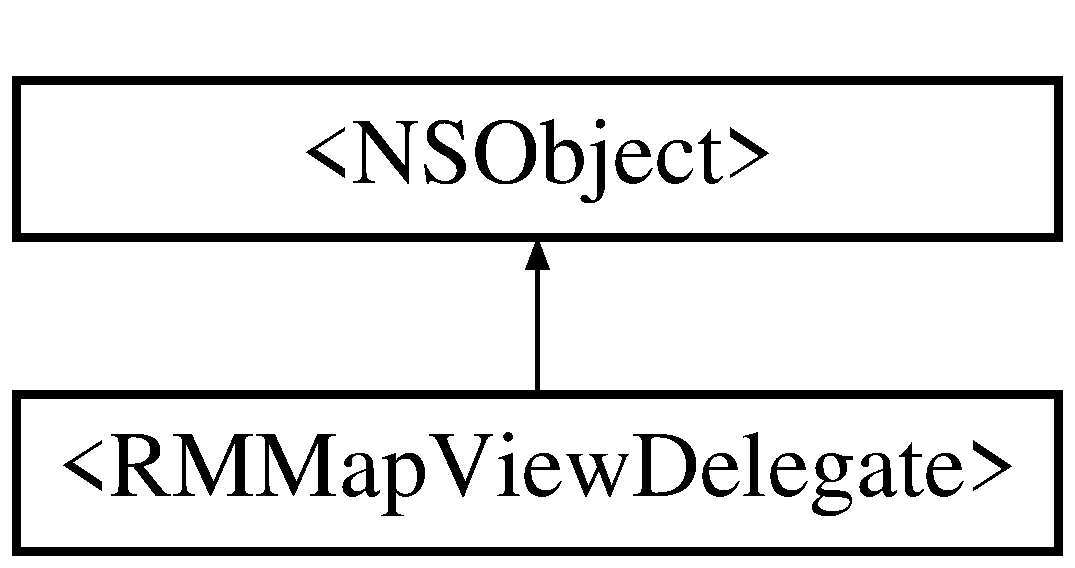
\includegraphics[height=2.000000cm]{protocol_r_m_map_view_delegate-p}
\end{center}
\end{figure}
\subsection*{Instance Methods}
\begin{DoxyCompactItemize}
\item 
(void) -\/ \hyperlink{protocol_r_m_map_view_delegate-p_a9b10956deeb8c0aeea94459bcb7b64b3}{after\-Map\-Move\-:}
\item 
(void) -\/ \hyperlink{protocol_r_m_map_view_delegate-p_a29d89b73151a5664e0757a1d36f93bdc}{after\-Map\-Rotate\-:to\-Angle\-:}
\item 
(void) -\/ \hyperlink{protocol_r_m_map_view_delegate-p_ab543918d0dfc6867db316eb66c460a83}{after\-Map\-Touch\-:}
\item 
(void) -\/ \hyperlink{protocol_r_m_map_view_delegate-p_a7785a3e85147f25316911d1cfaba276f}{after\-Map\-Zoom\-:by\-Factor\-:near\-:}
\item 
(void) -\/ \hyperlink{protocol_r_m_map_view_delegate-p_a020ebef5aa265d5452eecfa2eb4bda67}{before\-Map\-Move\-:}
\item 
(void) -\/ \hyperlink{protocol_r_m_map_view_delegate-p_a7e359b6183df46871ca7ffcb1f16cd59}{before\-Map\-Rotate\-:from\-Angle\-:}
\item 
(void) -\/ \hyperlink{protocol_r_m_map_view_delegate-p_a4e2099bacfe277f836c3e3fc4a93380d}{before\-Map\-Zoom\-:by\-Factor\-:near\-:}
\item 
(void) -\/ \hyperlink{protocol_r_m_map_view_delegate-p_a99bff74285b7262100f01a88eba695f5}{double\-Tap\-On\-Map\-:\-At\-:}
\item 
(void) -\/ \hyperlink{protocol_r_m_map_view_delegate-p_aaa7e0809e8b6761b3b84b717e2e1a251}{map\-View\-:did\-Drag\-Marker\-:with\-Event\-:}
\item 
(B\-O\-O\-L) -\/ \hyperlink{protocol_r_m_map_view_delegate-p_a02978876a2f774fc8165d0361dc52e90}{map\-View\-:should\-Drag\-Marker\-:with\-Event\-:}
\item 
(void) -\/ \hyperlink{protocol_r_m_map_view_delegate-p_a2ceb25e49bf55ddfe0f143148bf38396}{map\-View\-Region\-Did\-Change\-:}
\item 
(void) -\/ \hyperlink{protocol_r_m_map_view_delegate-p_ae8c30f1096a3524c51d6dd9e7da8a579}{single\-Tap\-On\-Map\-:\-At\-:}
\item 
(void) -\/ \hyperlink{protocol_r_m_map_view_delegate-p_a63f6c30db8812335f3a69cec9ef09783}{tap\-On\-Label\-For\-Marker\-:on\-Map\-:}
\item 
(void) -\/ \hyperlink{protocol_r_m_map_view_delegate-p_aca2e3042ef2bd1c8706c229f281730fc}{tap\-On\-Label\-For\-Marker\-:on\-Map\-:on\-Layer\-:}
\item 
(void) -\/ \hyperlink{protocol_r_m_map_view_delegate-p_aca0a4ab85c0220a9c2552e6cf1bd62c5}{tap\-On\-Marker\-:on\-Map\-:}
\end{DoxyCompactItemize}


\subsection{详细描述}
Use this for notifications of map panning, zooming, and taps on the \hyperlink{interface_r_m_map_view}{R\-M\-Map\-View}. 

\subsection{Method Documentation}
\hypertarget{protocol_r_m_map_view_delegate-p_a9b10956deeb8c0aeea94459bcb7b64b3}{\index{R\-M\-Map\-View\-Delegate-\/p@{R\-M\-Map\-View\-Delegate-\/p}!after\-Map\-Move\-:@{after\-Map\-Move\-:}}
\index{after\-Map\-Move\-:@{after\-Map\-Move\-:}!RMMapViewDelegate-p@{R\-M\-Map\-View\-Delegate-\/p}}
\subsubsection[{after\-Map\-Move\-:}]{\setlength{\rightskip}{0pt plus 5cm}-\/ (void) after\-Map\-Move\-: 
\begin{DoxyParamCaption}
\item[{({\bf R\-M\-Map\-View} $\ast$)}]{map}
\end{DoxyParamCaption}
\hspace{0.3cm}{\ttfamily [optional]}}}\label{protocol_r_m_map_view_delegate-p_a9b10956deeb8c0aeea94459bcb7b64b3}
\hypertarget{protocol_r_m_map_view_delegate-p_a29d89b73151a5664e0757a1d36f93bdc}{\index{R\-M\-Map\-View\-Delegate-\/p@{R\-M\-Map\-View\-Delegate-\/p}!after\-Map\-Rotate\-:to\-Angle\-:@{after\-Map\-Rotate\-:to\-Angle\-:}}
\index{after\-Map\-Rotate\-:to\-Angle\-:@{after\-Map\-Rotate\-:to\-Angle\-:}!RMMapViewDelegate-p@{R\-M\-Map\-View\-Delegate-\/p}}
\subsubsection[{after\-Map\-Rotate\-:to\-Angle\-:}]{\setlength{\rightskip}{0pt plus 5cm}-\/ (void) after\-Map\-Rotate\-: 
\begin{DoxyParamCaption}
\item[{({\bf R\-M\-Map\-View} $\ast$)}]{map}
\item[{toAngle:(C\-G\-Float)}]{angle}
\end{DoxyParamCaption}
\hspace{0.3cm}{\ttfamily [optional]}}}\label{protocol_r_m_map_view_delegate-p_a29d89b73151a5664e0757a1d36f93bdc}
\hypertarget{protocol_r_m_map_view_delegate-p_ab543918d0dfc6867db316eb66c460a83}{\index{R\-M\-Map\-View\-Delegate-\/p@{R\-M\-Map\-View\-Delegate-\/p}!after\-Map\-Touch\-:@{after\-Map\-Touch\-:}}
\index{after\-Map\-Touch\-:@{after\-Map\-Touch\-:}!RMMapViewDelegate-p@{R\-M\-Map\-View\-Delegate-\/p}}
\subsubsection[{after\-Map\-Touch\-:}]{\setlength{\rightskip}{0pt plus 5cm}-\/ (void) after\-Map\-Touch\-: 
\begin{DoxyParamCaption}
\item[{({\bf R\-M\-Map\-View} $\ast$)}]{map}
\end{DoxyParamCaption}
\hspace{0.3cm}{\ttfamily [optional]}}}\label{protocol_r_m_map_view_delegate-p_ab543918d0dfc6867db316eb66c460a83}
\hypertarget{protocol_r_m_map_view_delegate-p_a7785a3e85147f25316911d1cfaba276f}{\index{R\-M\-Map\-View\-Delegate-\/p@{R\-M\-Map\-View\-Delegate-\/p}!after\-Map\-Zoom\-:by\-Factor\-:near\-:@{after\-Map\-Zoom\-:by\-Factor\-:near\-:}}
\index{after\-Map\-Zoom\-:by\-Factor\-:near\-:@{after\-Map\-Zoom\-:by\-Factor\-:near\-:}!RMMapViewDelegate-p@{R\-M\-Map\-View\-Delegate-\/p}}
\subsubsection[{after\-Map\-Zoom\-:by\-Factor\-:near\-:}]{\setlength{\rightskip}{0pt plus 5cm}-\/ (void) after\-Map\-Zoom\-: 
\begin{DoxyParamCaption}
\item[{({\bf R\-M\-Map\-View} $\ast$)}]{map}
\item[{byFactor:(float)}]{zoom\-Factor}
\item[{near:(C\-G\-Point)}]{center}
\end{DoxyParamCaption}
\hspace{0.3cm}{\ttfamily [optional]}}}\label{protocol_r_m_map_view_delegate-p_a7785a3e85147f25316911d1cfaba276f}
\hypertarget{protocol_r_m_map_view_delegate-p_a020ebef5aa265d5452eecfa2eb4bda67}{\index{R\-M\-Map\-View\-Delegate-\/p@{R\-M\-Map\-View\-Delegate-\/p}!before\-Map\-Move\-:@{before\-Map\-Move\-:}}
\index{before\-Map\-Move\-:@{before\-Map\-Move\-:}!RMMapViewDelegate-p@{R\-M\-Map\-View\-Delegate-\/p}}
\subsubsection[{before\-Map\-Move\-:}]{\setlength{\rightskip}{0pt plus 5cm}-\/ (void) before\-Map\-Move\-: 
\begin{DoxyParamCaption}
\item[{({\bf R\-M\-Map\-View} $\ast$)}]{map}
\end{DoxyParamCaption}
\hspace{0.3cm}{\ttfamily [optional]}}}\label{protocol_r_m_map_view_delegate-p_a020ebef5aa265d5452eecfa2eb4bda67}
\hypertarget{protocol_r_m_map_view_delegate-p_a7e359b6183df46871ca7ffcb1f16cd59}{\index{R\-M\-Map\-View\-Delegate-\/p@{R\-M\-Map\-View\-Delegate-\/p}!before\-Map\-Rotate\-:from\-Angle\-:@{before\-Map\-Rotate\-:from\-Angle\-:}}
\index{before\-Map\-Rotate\-:from\-Angle\-:@{before\-Map\-Rotate\-:from\-Angle\-:}!RMMapViewDelegate-p@{R\-M\-Map\-View\-Delegate-\/p}}
\subsubsection[{before\-Map\-Rotate\-:from\-Angle\-:}]{\setlength{\rightskip}{0pt plus 5cm}-\/ (void) before\-Map\-Rotate\-: 
\begin{DoxyParamCaption}
\item[{({\bf R\-M\-Map\-View} $\ast$)}]{map}
\item[{fromAngle:(C\-G\-Float)}]{angle}
\end{DoxyParamCaption}
\hspace{0.3cm}{\ttfamily [optional]}}}\label{protocol_r_m_map_view_delegate-p_a7e359b6183df46871ca7ffcb1f16cd59}
\hypertarget{protocol_r_m_map_view_delegate-p_a4e2099bacfe277f836c3e3fc4a93380d}{\index{R\-M\-Map\-View\-Delegate-\/p@{R\-M\-Map\-View\-Delegate-\/p}!before\-Map\-Zoom\-:by\-Factor\-:near\-:@{before\-Map\-Zoom\-:by\-Factor\-:near\-:}}
\index{before\-Map\-Zoom\-:by\-Factor\-:near\-:@{before\-Map\-Zoom\-:by\-Factor\-:near\-:}!RMMapViewDelegate-p@{R\-M\-Map\-View\-Delegate-\/p}}
\subsubsection[{before\-Map\-Zoom\-:by\-Factor\-:near\-:}]{\setlength{\rightskip}{0pt plus 5cm}-\/ (void) before\-Map\-Zoom\-: 
\begin{DoxyParamCaption}
\item[{({\bf R\-M\-Map\-View} $\ast$)}]{map}
\item[{byFactor:(float)}]{zoom\-Factor}
\item[{near:(C\-G\-Point)}]{center}
\end{DoxyParamCaption}
\hspace{0.3cm}{\ttfamily [optional]}}}\label{protocol_r_m_map_view_delegate-p_a4e2099bacfe277f836c3e3fc4a93380d}
\hypertarget{protocol_r_m_map_view_delegate-p_a99bff74285b7262100f01a88eba695f5}{\index{R\-M\-Map\-View\-Delegate-\/p@{R\-M\-Map\-View\-Delegate-\/p}!double\-Tap\-On\-Map\-:\-At\-:@{double\-Tap\-On\-Map\-:\-At\-:}}
\index{double\-Tap\-On\-Map\-:\-At\-:@{double\-Tap\-On\-Map\-:\-At\-:}!RMMapViewDelegate-p@{R\-M\-Map\-View\-Delegate-\/p}}
\subsubsection[{double\-Tap\-On\-Map\-:\-At\-:}]{\setlength{\rightskip}{0pt plus 5cm}-\/ (void) double\-Tap\-On\-Map\-: 
\begin{DoxyParamCaption}
\item[{({\bf R\-M\-Map\-View} $\ast$)}]{map}
\item[{At:(C\-G\-Point)}]{point}
\end{DoxyParamCaption}
\hspace{0.3cm}{\ttfamily [optional]}}}\label{protocol_r_m_map_view_delegate-p_a99bff74285b7262100f01a88eba695f5}
\hypertarget{protocol_r_m_map_view_delegate-p_aaa7e0809e8b6761b3b84b717e2e1a251}{\index{R\-M\-Map\-View\-Delegate-\/p@{R\-M\-Map\-View\-Delegate-\/p}!map\-View\-:did\-Drag\-Marker\-:with\-Event\-:@{map\-View\-:did\-Drag\-Marker\-:with\-Event\-:}}
\index{map\-View\-:did\-Drag\-Marker\-:with\-Event\-:@{map\-View\-:did\-Drag\-Marker\-:with\-Event\-:}!RMMapViewDelegate-p@{R\-M\-Map\-View\-Delegate-\/p}}
\subsubsection[{map\-View\-:did\-Drag\-Marker\-:with\-Event\-:}]{\setlength{\rightskip}{0pt plus 5cm}-\/ (void) map\-View\-: 
\begin{DoxyParamCaption}
\item[{({\bf R\-M\-Map\-View} $\ast$)}]{map}
\item[{didDragMarker:({\bf R\-M\-Marker} $\ast$)}]{marker}
\item[{withEvent:(U\-I\-Event $\ast$)}]{event}
\end{DoxyParamCaption}
\hspace{0.3cm}{\ttfamily [optional]}}}\label{protocol_r_m_map_view_delegate-p_aaa7e0809e8b6761b3b84b717e2e1a251}
\hypertarget{protocol_r_m_map_view_delegate-p_a02978876a2f774fc8165d0361dc52e90}{\index{R\-M\-Map\-View\-Delegate-\/p@{R\-M\-Map\-View\-Delegate-\/p}!map\-View\-:should\-Drag\-Marker\-:with\-Event\-:@{map\-View\-:should\-Drag\-Marker\-:with\-Event\-:}}
\index{map\-View\-:should\-Drag\-Marker\-:with\-Event\-:@{map\-View\-:should\-Drag\-Marker\-:with\-Event\-:}!RMMapViewDelegate-p@{R\-M\-Map\-View\-Delegate-\/p}}
\subsubsection[{map\-View\-:should\-Drag\-Marker\-:with\-Event\-:}]{\setlength{\rightskip}{0pt plus 5cm}-\/ (B\-O\-O\-L) map\-View\-: 
\begin{DoxyParamCaption}
\item[{({\bf R\-M\-Map\-View} $\ast$)}]{map}
\item[{shouldDragMarker:({\bf R\-M\-Marker} $\ast$)}]{marker}
\item[{withEvent:(U\-I\-Event $\ast$)}]{event}
\end{DoxyParamCaption}
\hspace{0.3cm}{\ttfamily [optional]}}}\label{protocol_r_m_map_view_delegate-p_a02978876a2f774fc8165d0361dc52e90}
\hypertarget{protocol_r_m_map_view_delegate-p_a2ceb25e49bf55ddfe0f143148bf38396}{\index{R\-M\-Map\-View\-Delegate-\/p@{R\-M\-Map\-View\-Delegate-\/p}!map\-View\-Region\-Did\-Change\-:@{map\-View\-Region\-Did\-Change\-:}}
\index{map\-View\-Region\-Did\-Change\-:@{map\-View\-Region\-Did\-Change\-:}!RMMapViewDelegate-p@{R\-M\-Map\-View\-Delegate-\/p}}
\subsubsection[{map\-View\-Region\-Did\-Change\-:}]{\setlength{\rightskip}{0pt plus 5cm}-\/ (void) map\-View\-Region\-Did\-Change\-: 
\begin{DoxyParamCaption}
\item[{({\bf R\-M\-Map\-View} $\ast$)}]{map\-View}
\end{DoxyParamCaption}
\hspace{0.3cm}{\ttfamily [optional]}}}\label{protocol_r_m_map_view_delegate-p_a2ceb25e49bf55ddfe0f143148bf38396}
\hypertarget{protocol_r_m_map_view_delegate-p_ae8c30f1096a3524c51d6dd9e7da8a579}{\index{R\-M\-Map\-View\-Delegate-\/p@{R\-M\-Map\-View\-Delegate-\/p}!single\-Tap\-On\-Map\-:\-At\-:@{single\-Tap\-On\-Map\-:\-At\-:}}
\index{single\-Tap\-On\-Map\-:\-At\-:@{single\-Tap\-On\-Map\-:\-At\-:}!RMMapViewDelegate-p@{R\-M\-Map\-View\-Delegate-\/p}}
\subsubsection[{single\-Tap\-On\-Map\-:\-At\-:}]{\setlength{\rightskip}{0pt plus 5cm}-\/ (void) single\-Tap\-On\-Map\-: 
\begin{DoxyParamCaption}
\item[{({\bf R\-M\-Map\-View} $\ast$)}]{map}
\item[{At:(C\-G\-Point)}]{point}
\end{DoxyParamCaption}
\hspace{0.3cm}{\ttfamily [optional]}}}\label{protocol_r_m_map_view_delegate-p_ae8c30f1096a3524c51d6dd9e7da8a579}
\hypertarget{protocol_r_m_map_view_delegate-p_a63f6c30db8812335f3a69cec9ef09783}{\index{R\-M\-Map\-View\-Delegate-\/p@{R\-M\-Map\-View\-Delegate-\/p}!tap\-On\-Label\-For\-Marker\-:on\-Map\-:@{tap\-On\-Label\-For\-Marker\-:on\-Map\-:}}
\index{tap\-On\-Label\-For\-Marker\-:on\-Map\-:@{tap\-On\-Label\-For\-Marker\-:on\-Map\-:}!RMMapViewDelegate-p@{R\-M\-Map\-View\-Delegate-\/p}}
\subsubsection[{tap\-On\-Label\-For\-Marker\-:on\-Map\-:}]{\setlength{\rightskip}{0pt plus 5cm}-\/ (void) tap\-On\-Label\-For\-Marker\-: 
\begin{DoxyParamCaption}
\item[{({\bf R\-M\-Marker} $\ast$)}]{marker}
\item[{onMap:({\bf R\-M\-Map\-View} $\ast$)}]{map}
\end{DoxyParamCaption}
\hspace{0.3cm}{\ttfamily [optional]}}}\label{protocol_r_m_map_view_delegate-p_a63f6c30db8812335f3a69cec9ef09783}
\hypertarget{protocol_r_m_map_view_delegate-p_aca2e3042ef2bd1c8706c229f281730fc}{\index{R\-M\-Map\-View\-Delegate-\/p@{R\-M\-Map\-View\-Delegate-\/p}!tap\-On\-Label\-For\-Marker\-:on\-Map\-:on\-Layer\-:@{tap\-On\-Label\-For\-Marker\-:on\-Map\-:on\-Layer\-:}}
\index{tap\-On\-Label\-For\-Marker\-:on\-Map\-:on\-Layer\-:@{tap\-On\-Label\-For\-Marker\-:on\-Map\-:on\-Layer\-:}!RMMapViewDelegate-p@{R\-M\-Map\-View\-Delegate-\/p}}
\subsubsection[{tap\-On\-Label\-For\-Marker\-:on\-Map\-:on\-Layer\-:}]{\setlength{\rightskip}{0pt plus 5cm}-\/ (void) tap\-On\-Label\-For\-Marker\-: 
\begin{DoxyParamCaption}
\item[{({\bf R\-M\-Marker} $\ast$)}]{marker}
\item[{onMap:({\bf R\-M\-Map\-View} $\ast$)}]{map}
\item[{onLayer:(C\-A\-Layer $\ast$)}]{layer}
\end{DoxyParamCaption}
\hspace{0.3cm}{\ttfamily [optional]}}}\label{protocol_r_m_map_view_delegate-p_aca2e3042ef2bd1c8706c229f281730fc}
\hypertarget{protocol_r_m_map_view_delegate-p_aca0a4ab85c0220a9c2552e6cf1bd62c5}{\index{R\-M\-Map\-View\-Delegate-\/p@{R\-M\-Map\-View\-Delegate-\/p}!tap\-On\-Marker\-:on\-Map\-:@{tap\-On\-Marker\-:on\-Map\-:}}
\index{tap\-On\-Marker\-:on\-Map\-:@{tap\-On\-Marker\-:on\-Map\-:}!RMMapViewDelegate-p@{R\-M\-Map\-View\-Delegate-\/p}}
\subsubsection[{tap\-On\-Marker\-:on\-Map\-:}]{\setlength{\rightskip}{0pt plus 5cm}-\/ (void) tap\-On\-Marker\-: 
\begin{DoxyParamCaption}
\item[{({\bf R\-M\-Marker} $\ast$)}]{marker}
\item[{onMap:({\bf R\-M\-Map\-View} $\ast$)}]{map}
\end{DoxyParamCaption}
\hspace{0.3cm}{\ttfamily [optional]}}}\label{protocol_r_m_map_view_delegate-p_aca0a4ab85c0220a9c2552e6cf1bd62c5}


该协议的文档由以下文件生成\-:\begin{DoxyCompactItemize}
\item 
Map/\hyperlink{_r_m_map_view_delegate_8h}{R\-M\-Map\-View\-Delegate.\-h}\end{DoxyCompactItemize}

\hypertarget{interface_r_m_marker}{\section{R\-M\-Marker类 参考}
\label{interface_r_m_marker}\index{R\-M\-Marker@{R\-M\-Marker}}
}


one marker drawn on the map.  




{\ttfamily \#import $<$R\-M\-Marker.\-h$>$}

类 R\-M\-Marker 继承关系图\-:\begin{figure}[H]
\begin{center}
\leavevmode
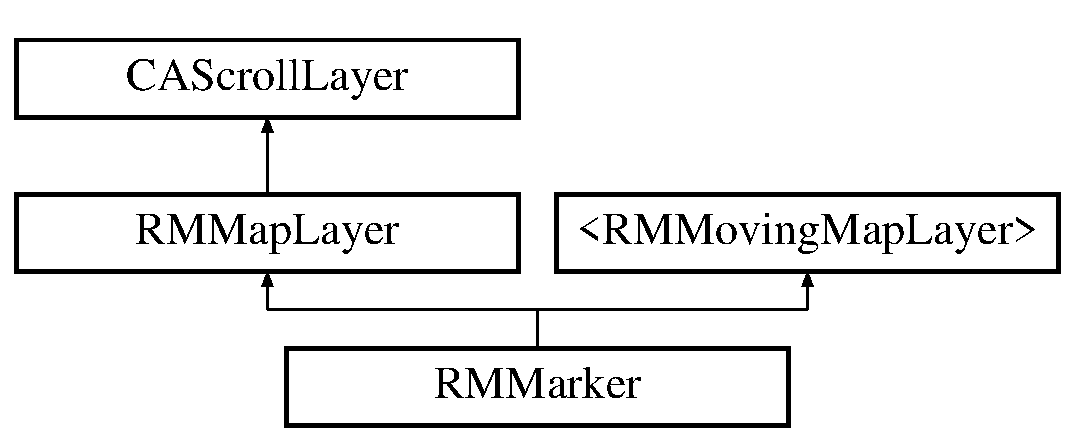
\includegraphics[height=3.000000cm]{interface_r_m_marker}
\end{center}
\end{figure}
\subsection*{Instance Methods}
\begin{DoxyCompactItemize}
\item 
(void) -\/ \hyperlink{interface_r_m_marker_a74563af9b6eaf61603636c1202457ecb}{change\-Label\-Using\-Text\-:}
\begin{DoxyCompactList}\small\item\em changes the label\-View to a U\-I\-Label with supplied \#text and default marker font, using existing text foreground/background color. \end{DoxyCompactList}\item 
(void) -\/ \hyperlink{interface_r_m_marker_a5dd4fe76d126bbab97f392aeb9bfb3ec}{change\-Label\-Using\-Text\-:font\-:foreground\-Color\-:background\-Color\-:}
\begin{DoxyCompactList}\small\item\em changes the label\-View to a U\-I\-Label with supplied \#text and default marker font, changing this marker's text foreground/background colors for this and future text strings. \end{DoxyCompactList}\item 
(void) -\/ \hyperlink{interface_r_m_marker_a456cace65c4d3399d7f3909baa4028d5}{change\-Label\-Using\-Text\-:position\-:}
\begin{DoxyCompactList}\small\item\em changes the label\-View to a U\-I\-Label with supplied \#text and default marker font, positioning the text some weird way i don't understand yet. Uses existing text color/background color. \end{DoxyCompactList}\item 
(void) -\/ \hyperlink{interface_r_m_marker_a2de0b0fbed16e70eaa0aeee0d631a3e6}{change\-Label\-Using\-Text\-:position\-:font\-:foreground\-Color\-:background\-Color\-:}
\begin{DoxyCompactList}\small\item\em changes the label\-View to a U\-I\-Label with supplied \#text and default marker font, changing this marker's text foreground/background colors for this and future text strings; modifies position as in \hyperlink{interface_r_m_marker_a74563af9b6eaf61603636c1202457ecb}{change\-Label\-Using\-Text\-:}position. \end{DoxyCompactList}\item 
(void) -\/ \hyperlink{interface_r_m_marker_a9ed3651f45b68ee08af321a7c1d53b30}{dealloc}
\item 
(void) -\/ \hyperlink{interface_r_m_marker_a59b781fa30a11764bfb378650a20b01c}{hide\-Label}
\item 
(id) -\/ \hyperlink{interface_r_m_marker_ae896ffbfa063f34d49741f540b3f9201}{init}{\ttfamily  \mbox{[}implementation\mbox{]}}
\item 
(id) -\/ \hyperlink{interface_r_m_marker_a89dd90402903576e798ec555d5bf5ff5}{init\-With\-U\-I\-Image\-:}
\begin{DoxyCompactList}\small\item\em returns \hyperlink{interface_r_m_marker}{R\-M\-Marker} initialized with \#image, and the default anchor point (0.\-5, 0.\-5) \end{DoxyCompactList}\item 
(id) -\/ \hyperlink{interface_r_m_marker_a37ad8cd65c9597bb5296e784503f92e0}{init\-With\-U\-I\-Image\-:anchor\-Point\-:}
\begin{DoxyCompactList}\small\item\em returns \hyperlink{interface_r_m_marker}{R\-M\-Marker} initialized with provided image and anchor\-Point. \end{DoxyCompactList}\item 
(void) -\/ \hyperlink{interface_r_m_marker_a96b0d02976d98b17a2d8383d9cb4c807}{move\-By\-:}{\ttfamily  \mbox{[}implementation\mbox{]}}
\item 
(void) -\/ \hyperlink{interface_r_m_marker_a906621c61e31e6759d977fe1086aff44}{replace\-U\-I\-Image\-:}
\item 
(void) -\/ \hyperlink{interface_r_m_marker_a2e50edfeb2efe837bcc1fb5962c874d9}{replace\-U\-I\-Image\-:anchor\-Point\-:}
\item 
(void) -\/ \hyperlink{interface_r_m_marker_a1a507346790dbd6b4d9f131362bb167e}{set\-Label\-:}{\ttfamily  \mbox{[}implementation\mbox{]}}
\item 
(void) -\/ \hyperlink{interface_r_m_marker_ac3cb506fdb758c68bbfb31dbc20ced0a}{show\-Label}
\item 
(void) -\/ \hyperlink{interface_r_m_marker_a0a6f1212f47120f99be764ed14b074fb}{toggle\-Label}
\item 
(void) -\/ \hyperlink{interface_r_m_marker_ad98fa242aceef563743c13963d8a79ca}{zoom\-By\-Factor\-:near\-:}{\ttfamily  \mbox{[}implementation\mbox{]}}
\end{DoxyCompactItemize}
\subsection*{Class Methods}
\begin{DoxyCompactItemize}
\item 
(U\-I\-Font $\ast$) + \hyperlink{interface_r_m_marker_a643af8a0d5028b5df597f2ab812e5ea8}{default\-Font}
\begin{DoxyCompactList}\small\item\em the font used for labels when another font is not explicitly requested; currently \mbox{[}U\-I\-Font system\-Font\-Of\-Size\-:15\mbox{]} \end{DoxyCompactList}\end{DoxyCompactItemize}
\subsection*{属性}
\begin{DoxyCompactItemize}
\item 
N\-S\-Object $\ast$ \hyperlink{interface_r_m_marker_ae31cf29f5239ae3410a9aa18f7831949}{data}
\begin{DoxyCompactList}\small\item\em provided for storage of arbitrary user data \end{DoxyCompactList}\item 
B\-O\-O\-L \hyperlink{interface_r_m_marker_abdaaec7c6a67902e90e95c072ca19f0a}{enable\-Dragging}
\item 
B\-O\-O\-L \hyperlink{interface_r_m_marker_afba7d967f0f18ec0d5dc668a9a3e27ff}{enable\-Rotation}
\item 
U\-I\-View $\ast$ \hyperlink{interface_r_m_marker_a8eb1ce06dea5a1c89feb3b7b8c7de25c}{label}
\begin{DoxyCompactList}\small\item\em Text label, visible by default if it has content, but not required. \end{DoxyCompactList}\item 
\hyperlink{struct_r_m_projected_point}{R\-M\-Projected\-Point} \hyperlink{interface_r_m_marker_ac810ea4f4af07c3b3fc5300fe40eebd5}{projected\-Location}
\begin{DoxyCompactList}\small\item\em expressed in projected meters. The anchor\-Point of the image is plotted here. \end{DoxyCompactList}\item 
U\-I\-Color $\ast$ \hyperlink{interface_r_m_marker_a75d470aa3039d2fc8212550c7e18a401}{text\-Background\-Color}
\item 
U\-I\-Color $\ast$ \hyperlink{interface_r_m_marker_a8c17bd3321a486c5738c5b7521e07022}{text\-Foreground\-Color}
\end{DoxyCompactItemize}


\subsection{详细描述}
one marker drawn on the map. 

Note that \hyperlink{interface_r_m_marker}{R\-M\-Marker} ultimately descends from C\-A\-Layer, and has an image contents. \hyperlink{interface_r_m_marker}{R\-M\-Marker} inherits \char`\"{}position\char`\"{} and \char`\"{}anchor\-Point\char`\"{} from C\-A\-Layer. 

\subsection{Method Documentation}
\hypertarget{interface_r_m_marker_a74563af9b6eaf61603636c1202457ecb}{\index{R\-M\-Marker@{R\-M\-Marker}!change\-Label\-Using\-Text\-:@{change\-Label\-Using\-Text\-:}}
\index{change\-Label\-Using\-Text\-:@{change\-Label\-Using\-Text\-:}!RMMarker@{R\-M\-Marker}}
\subsubsection[{change\-Label\-Using\-Text\-:}]{\setlength{\rightskip}{0pt plus 5cm}-\/ (void) change\-Label\-Using\-Text\-: 
\begin{DoxyParamCaption}
\item[{(N\-S\-String$\ast$)}]{text}
\end{DoxyParamCaption}
}}\label{interface_r_m_marker_a74563af9b6eaf61603636c1202457ecb}


changes the label\-View to a U\-I\-Label with supplied \#text and default marker font, using existing text foreground/background color. 

\begin{DoxyRefDesc}{Bug}
\item[\hyperlink{bug__bug000026}{Bug}]hardcoded font name \end{DoxyRefDesc}
\hypertarget{interface_r_m_marker_a5dd4fe76d126bbab97f392aeb9bfb3ec}{\index{R\-M\-Marker@{R\-M\-Marker}!change\-Label\-Using\-Text\-:font\-:foreground\-Color\-:background\-Color\-:@{change\-Label\-Using\-Text\-:font\-:foreground\-Color\-:background\-Color\-:}}
\index{change\-Label\-Using\-Text\-:font\-:foreground\-Color\-:background\-Color\-:@{change\-Label\-Using\-Text\-:font\-:foreground\-Color\-:background\-Color\-:}!RMMarker@{R\-M\-Marker}}
\subsubsection[{change\-Label\-Using\-Text\-:font\-:foreground\-Color\-:background\-Color\-:}]{\setlength{\rightskip}{0pt plus 5cm}-\/ (void) {\bf change\-Label\-Using\-Text\-:} 
\begin{DoxyParamCaption}
\item[{(N\-S\-String$\ast$)}]{text}
\item[{font:(U\-I\-Font$\ast$)}]{font}
\item[{foregroundColor:(U\-I\-Color$\ast$)}]{text\-Color}
\item[{backgroundColor:(U\-I\-Color$\ast$)}]{background\-Color}
\end{DoxyParamCaption}
}}\label{interface_r_m_marker_a5dd4fe76d126bbab97f392aeb9bfb3ec}


changes the label\-View to a U\-I\-Label with supplied \#text and default marker font, changing this marker's text foreground/background colors for this and future text strings. 

\hypertarget{interface_r_m_marker_a456cace65c4d3399d7f3909baa4028d5}{\index{R\-M\-Marker@{R\-M\-Marker}!change\-Label\-Using\-Text\-:position\-:@{change\-Label\-Using\-Text\-:position\-:}}
\index{change\-Label\-Using\-Text\-:position\-:@{change\-Label\-Using\-Text\-:position\-:}!RMMarker@{R\-M\-Marker}}
\subsubsection[{change\-Label\-Using\-Text\-:position\-:}]{\setlength{\rightskip}{0pt plus 5cm}-\/ (void) {\bf change\-Label\-Using\-Text\-:} 
\begin{DoxyParamCaption}
\item[{(N\-S\-String$\ast$)}]{text}
\item[{position:(C\-G\-Point)}]{position}
\end{DoxyParamCaption}
}}\label{interface_r_m_marker_a456cace65c4d3399d7f3909baa4028d5}


changes the label\-View to a U\-I\-Label with supplied \#text and default marker font, positioning the text some weird way i don't understand yet. Uses existing text color/background color. 

\hypertarget{interface_r_m_marker_a2de0b0fbed16e70eaa0aeee0d631a3e6}{\index{R\-M\-Marker@{R\-M\-Marker}!change\-Label\-Using\-Text\-:position\-:font\-:foreground\-Color\-:background\-Color\-:@{change\-Label\-Using\-Text\-:position\-:font\-:foreground\-Color\-:background\-Color\-:}}
\index{change\-Label\-Using\-Text\-:position\-:font\-:foreground\-Color\-:background\-Color\-:@{change\-Label\-Using\-Text\-:position\-:font\-:foreground\-Color\-:background\-Color\-:}!RMMarker@{R\-M\-Marker}}
\subsubsection[{change\-Label\-Using\-Text\-:position\-:font\-:foreground\-Color\-:background\-Color\-:}]{\setlength{\rightskip}{0pt plus 5cm}-\/ (void) {\bf change\-Label\-Using\-Text\-:} 
\begin{DoxyParamCaption}
\item[{(N\-S\-String$\ast$)}]{text}
\item[{position:(C\-G\-Point)}]{position}
\item[{font:(U\-I\-Font$\ast$)}]{font}
\item[{foregroundColor:(U\-I\-Color$\ast$)}]{text\-Color}
\item[{backgroundColor:(U\-I\-Color$\ast$)}]{background\-Color}
\end{DoxyParamCaption}
}}\label{interface_r_m_marker_a2de0b0fbed16e70eaa0aeee0d631a3e6}


changes the label\-View to a U\-I\-Label with supplied \#text and default marker font, changing this marker's text foreground/background colors for this and future text strings; modifies position as in \hyperlink{interface_r_m_marker_a74563af9b6eaf61603636c1202457ecb}{change\-Label\-Using\-Text\-:}position. 



参考自 change\-Label\-Using\-Text\-:, change\-Label\-Using\-Text\-:font\-:foreground\-Color\-:background\-Color\-: , 以及 change\-Label\-Using\-Text\-:position\-:.

\hypertarget{interface_r_m_marker_a9ed3651f45b68ee08af321a7c1d53b30}{\index{R\-M\-Marker@{R\-M\-Marker}!dealloc@{dealloc}}
\index{dealloc@{dealloc}!RMMarker@{R\-M\-Marker}}
\subsubsection[{dealloc}]{\setlength{\rightskip}{0pt plus 5cm}-\/ (void) dealloc 
\begin{DoxyParamCaption}
{}
\end{DoxyParamCaption}
}}\label{interface_r_m_marker_a9ed3651f45b68ee08af321a7c1d53b30}
\hypertarget{interface_r_m_marker_a643af8a0d5028b5df597f2ab812e5ea8}{\index{R\-M\-Marker@{R\-M\-Marker}!default\-Font@{default\-Font}}
\index{default\-Font@{default\-Font}!RMMarker@{R\-M\-Marker}}
\subsubsection[{default\-Font}]{\setlength{\rightskip}{0pt plus 5cm}+ (U\-I\-Font $\ast$) default\-Font 
\begin{DoxyParamCaption}
{}
\end{DoxyParamCaption}
}}\label{interface_r_m_marker_a643af8a0d5028b5df597f2ab812e5ea8}


the font used for labels when another font is not explicitly requested; currently \mbox{[}U\-I\-Font system\-Font\-Of\-Size\-:15\mbox{]} 



参考自 change\-Label\-Using\-Text\-: , 以及 change\-Label\-Using\-Text\-:position\-:.

\hypertarget{interface_r_m_marker_a59b781fa30a11764bfb378650a20b01c}{\index{R\-M\-Marker@{R\-M\-Marker}!hide\-Label@{hide\-Label}}
\index{hide\-Label@{hide\-Label}!RMMarker@{R\-M\-Marker}}
\subsubsection[{hide\-Label}]{\setlength{\rightskip}{0pt plus 5cm}-\/ (void) hide\-Label 
\begin{DoxyParamCaption}
{}
\end{DoxyParamCaption}
}}\label{interface_r_m_marker_a59b781fa30a11764bfb378650a20b01c}


参考自 toggle\-Label.

\hypertarget{interface_r_m_marker_ae896ffbfa063f34d49741f540b3f9201}{\index{R\-M\-Marker@{R\-M\-Marker}!init@{init}}
\index{init@{init}!RMMarker@{R\-M\-Marker}}
\subsubsection[{init}]{\setlength{\rightskip}{0pt plus 5cm}-\/ (id) init 
\begin{DoxyParamCaption}
{}
\end{DoxyParamCaption}
\hspace{0.3cm}{\ttfamily [implementation]}}}\label{interface_r_m_marker_ae896ffbfa063f34d49741f540b3f9201}


重载 \hyperlink{interface_r_m_map_layer_a0ef1b877235bcaedb2929dae3bd92750}{R\-M\-Map\-Layer} .



参考自 init\-With\-U\-I\-Image\-:anchor\-Point\-:.

\hypertarget{interface_r_m_marker_a89dd90402903576e798ec555d5bf5ff5}{\index{R\-M\-Marker@{R\-M\-Marker}!init\-With\-U\-I\-Image\-:@{init\-With\-U\-I\-Image\-:}}
\index{init\-With\-U\-I\-Image\-:@{init\-With\-U\-I\-Image\-:}!RMMarker@{R\-M\-Marker}}
\subsubsection[{init\-With\-U\-I\-Image\-:}]{\setlength{\rightskip}{0pt plus 5cm}-\/ (id) init\-With\-U\-I\-Image\-: 
\begin{DoxyParamCaption}
\item[{(U\-I\-Image$\ast$)}]{image}
\end{DoxyParamCaption}
}}\label{interface_r_m_marker_a89dd90402903576e798ec555d5bf5ff5}


returns \hyperlink{interface_r_m_marker}{R\-M\-Marker} initialized with \#image, and the default anchor point (0.\-5, 0.\-5) 

\hypertarget{interface_r_m_marker_a37ad8cd65c9597bb5296e784503f92e0}{\index{R\-M\-Marker@{R\-M\-Marker}!init\-With\-U\-I\-Image\-:anchor\-Point\-:@{init\-With\-U\-I\-Image\-:anchor\-Point\-:}}
\index{init\-With\-U\-I\-Image\-:anchor\-Point\-:@{init\-With\-U\-I\-Image\-:anchor\-Point\-:}!RMMarker@{R\-M\-Marker}}
\subsubsection[{init\-With\-U\-I\-Image\-:anchor\-Point\-:}]{\setlength{\rightskip}{0pt plus 5cm}-\/ (id) {\bf init\-With\-U\-I\-Image\-:} 
\begin{DoxyParamCaption}
\item[{(U\-I\-Image$\ast$)}]{image}
\item[{anchorPoint:(C\-G\-Point)}]{anchor\-Point}
\end{DoxyParamCaption}
}}\label{interface_r_m_marker_a37ad8cd65c9597bb5296e784503f92e0}


returns \hyperlink{interface_r_m_marker}{R\-M\-Marker} initialized with provided image and anchor\-Point. 

\#anchor\-Point x and y range from 0 to 1, normalized to the width and height of image, referenced to upper left corner, y increasing top to bottom. To put the image's upper right corner on the marker's \hyperlink{interface_r_m_marker_ac810ea4f4af07c3b3fc5300fe40eebd5}{projected\-Location}, use an anchor point of (1.\-0, 0.\-0); 

参考自 init\-With\-U\-I\-Image\-:.

\hypertarget{interface_r_m_marker_a96b0d02976d98b17a2d8383d9cb4c807}{\index{R\-M\-Marker@{R\-M\-Marker}!move\-By\-:@{move\-By\-:}}
\index{move\-By\-:@{move\-By\-:}!RMMarker@{R\-M\-Marker}}
\subsubsection[{move\-By\-:}]{\setlength{\rightskip}{0pt plus 5cm}-\/ (void) move\-By\-: 
\begin{DoxyParamCaption}
\item[{(C\-G\-Size)}]{delta}
\end{DoxyParamCaption}
\hspace{0.3cm}{\ttfamily [implementation]}}}\label{interface_r_m_marker_a96b0d02976d98b17a2d8383d9cb4c807}


重载 \hyperlink{interface_r_m_map_layer_ac960944a80c596eb918531cf63c54c11}{R\-M\-Map\-Layer} .

\hypertarget{interface_r_m_marker_a906621c61e31e6759d977fe1086aff44}{\index{R\-M\-Marker@{R\-M\-Marker}!replace\-U\-I\-Image\-:@{replace\-U\-I\-Image\-:}}
\index{replace\-U\-I\-Image\-:@{replace\-U\-I\-Image\-:}!RMMarker@{R\-M\-Marker}}
\subsubsection[{replace\-U\-I\-Image\-:}]{\setlength{\rightskip}{0pt plus 5cm}-\/ (void) replace\-U\-I\-Image\-: 
\begin{DoxyParamCaption}
\item[{(U\-I\-Image$\ast$)}]{image}
\end{DoxyParamCaption}
}}\label{interface_r_m_marker_a906621c61e31e6759d977fe1086aff44}
\hypertarget{interface_r_m_marker_a2e50edfeb2efe837bcc1fb5962c874d9}{\index{R\-M\-Marker@{R\-M\-Marker}!replace\-U\-I\-Image\-:anchor\-Point\-:@{replace\-U\-I\-Image\-:anchor\-Point\-:}}
\index{replace\-U\-I\-Image\-:anchor\-Point\-:@{replace\-U\-I\-Image\-:anchor\-Point\-:}!RMMarker@{R\-M\-Marker}}
\subsubsection[{replace\-U\-I\-Image\-:anchor\-Point\-:}]{\setlength{\rightskip}{0pt plus 5cm}-\/ (void) {\bf replace\-U\-I\-Image\-:} 
\begin{DoxyParamCaption}
\item[{(U\-I\-Image$\ast$)}]{image}
\item[{anchorPoint:(C\-G\-Point)}]{anchor\-Point}
\end{DoxyParamCaption}
}}\label{interface_r_m_marker_a2e50edfeb2efe837bcc1fb5962c874d9}


参考自 replace\-U\-I\-Image\-:.

\hypertarget{interface_r_m_marker_a1a507346790dbd6b4d9f131362bb167e}{\index{R\-M\-Marker@{R\-M\-Marker}!set\-Label\-:@{set\-Label\-:}}
\index{set\-Label\-:@{set\-Label\-:}!RMMarker@{R\-M\-Marker}}
\subsubsection[{set\-Label\-:}]{\setlength{\rightskip}{0pt plus 5cm}-\/ (void) set\-Label\-: 
\begin{DoxyParamCaption}
\item[{(U\-I\-View$\ast$)}]{a\-View}
\end{DoxyParamCaption}
\hspace{0.3cm}{\ttfamily [implementation]}}}\label{interface_r_m_marker_a1a507346790dbd6b4d9f131362bb167e}


参考自 change\-Label\-Using\-Text\-:position\-:font\-:foreground\-Color\-:background\-Color\-:.

\hypertarget{interface_r_m_marker_ac3cb506fdb758c68bbfb31dbc20ced0a}{\index{R\-M\-Marker@{R\-M\-Marker}!show\-Label@{show\-Label}}
\index{show\-Label@{show\-Label}!RMMarker@{R\-M\-Marker}}
\subsubsection[{show\-Label}]{\setlength{\rightskip}{0pt plus 5cm}-\/ (void) show\-Label 
\begin{DoxyParamCaption}
{}
\end{DoxyParamCaption}
}}\label{interface_r_m_marker_ac3cb506fdb758c68bbfb31dbc20ced0a}


参考自 toggle\-Label.

\hypertarget{interface_r_m_marker_a0a6f1212f47120f99be764ed14b074fb}{\index{R\-M\-Marker@{R\-M\-Marker}!toggle\-Label@{toggle\-Label}}
\index{toggle\-Label@{toggle\-Label}!RMMarker@{R\-M\-Marker}}
\subsubsection[{toggle\-Label}]{\setlength{\rightskip}{0pt plus 5cm}-\/ (void) toggle\-Label 
\begin{DoxyParamCaption}
{}
\end{DoxyParamCaption}
}}\label{interface_r_m_marker_a0a6f1212f47120f99be764ed14b074fb}
\hypertarget{interface_r_m_marker_ad98fa242aceef563743c13963d8a79ca}{\index{R\-M\-Marker@{R\-M\-Marker}!zoom\-By\-Factor\-:near\-:@{zoom\-By\-Factor\-:near\-:}}
\index{zoom\-By\-Factor\-:near\-:@{zoom\-By\-Factor\-:near\-:}!RMMarker@{R\-M\-Marker}}
\subsubsection[{zoom\-By\-Factor\-:near\-:}]{\setlength{\rightskip}{0pt plus 5cm}-\/ (void) zoom\-By\-Factor\-: 
\begin{DoxyParamCaption}
\item[{(float)}]{zoom\-Factor}
\item[{near:(C\-G\-Point)}]{center}
\end{DoxyParamCaption}
\hspace{0.3cm}{\ttfamily [implementation]}}}\label{interface_r_m_marker_ad98fa242aceef563743c13963d8a79ca}


重载 \hyperlink{interface_r_m_map_layer_ae0e1f8c364aaca4ac39766fe14bbba07}{R\-M\-Map\-Layer} .



\subsection{属性说明}
\hypertarget{interface_r_m_marker_ae31cf29f5239ae3410a9aa18f7831949}{\index{R\-M\-Marker@{R\-M\-Marker}!data@{data}}
\index{data@{data}!RMMarker@{R\-M\-Marker}}
\subsubsection[{data}]{\setlength{\rightskip}{0pt plus 5cm}-\/ (N\-S\-Object $\ast$) data\hspace{0.3cm}{\ttfamily [read]}, {\ttfamily [write]}, {\ttfamily [nonatomic]}, {\ttfamily [retain]}}}\label{interface_r_m_marker_ae31cf29f5239ae3410a9aa18f7831949}


provided for storage of arbitrary user data 

\hypertarget{interface_r_m_marker_abdaaec7c6a67902e90e95c072ca19f0a}{\index{R\-M\-Marker@{R\-M\-Marker}!enable\-Dragging@{enable\-Dragging}}
\index{enable\-Dragging@{enable\-Dragging}!RMMarker@{R\-M\-Marker}}
\subsubsection[{enable\-Dragging}]{\setlength{\rightskip}{0pt plus 5cm}-\/ (B\-O\-O\-L) enable\-Dragging\hspace{0.3cm}{\ttfamily [read]}, {\ttfamily [write]}, {\ttfamily [atomic]}, {\ttfamily [assign]}}}\label{interface_r_m_marker_abdaaec7c6a67902e90e95c072ca19f0a}


参考自 init, move\-By\-: , 以及 zoom\-By\-Factor\-:near\-:.

\hypertarget{interface_r_m_marker_afba7d967f0f18ec0d5dc668a9a3e27ff}{\index{R\-M\-Marker@{R\-M\-Marker}!enable\-Rotation@{enable\-Rotation}}
\index{enable\-Rotation@{enable\-Rotation}!RMMarker@{R\-M\-Marker}}
\subsubsection[{enable\-Rotation}]{\setlength{\rightskip}{0pt plus 5cm}-\/ (B\-O\-O\-L) enable\-Rotation\hspace{0.3cm}{\ttfamily [read]}, {\ttfamily [write]}, {\ttfamily [atomic]}, {\ttfamily [assign]}}}\label{interface_r_m_marker_afba7d967f0f18ec0d5dc668a9a3e27ff}


参考自 R\-M\-Marker\-Manager\-::add\-Marker\-:at\-Projected\-Point\-:, init , 以及 R\-M\-Marker\-Manager\-::set\-Rotation\-:.

\hypertarget{interface_r_m_marker_a8eb1ce06dea5a1c89feb3b7b8c7de25c}{\index{R\-M\-Marker@{R\-M\-Marker}!label@{label}}
\index{label@{label}!RMMarker@{R\-M\-Marker}}
\subsubsection[{label}]{\setlength{\rightskip}{0pt plus 5cm}-\/ (U\-I\-View $\ast$) label\hspace{0.3cm}{\ttfamily [read]}, {\ttfamily [write]}, {\ttfamily [nonatomic]}, {\ttfamily [retain]}}}\label{interface_r_m_marker_a8eb1ce06dea5a1c89feb3b7b8c7de25c}


Text label, visible by default if it has content, but not required. 



参考自 hide\-Label, init, set\-Label\-:, show\-Label , 以及 toggle\-Label.

\hypertarget{interface_r_m_marker_ac810ea4f4af07c3b3fc5300fe40eebd5}{\index{R\-M\-Marker@{R\-M\-Marker}!projected\-Location@{projected\-Location}}
\index{projected\-Location@{projected\-Location}!RMMarker@{R\-M\-Marker}}
\subsubsection[{projected\-Location}]{\setlength{\rightskip}{0pt plus 5cm}-\/ ({\bf R\-M\-Projected\-Point}) projected\-Location\hspace{0.3cm}{\ttfamily [read]}, {\ttfamily [write]}, {\ttfamily [nonatomic]}, {\ttfamily [assign]}}}\label{interface_r_m_marker_ac810ea4f4af07c3b3fc5300fe40eebd5}


expressed in projected meters. The anchor\-Point of the image is plotted here. 



参考自 R\-M\-Layer\-Collection\-::layer\-Sort , 以及 R\-M\-Marker\-Manager\-::screen\-Coordinates\-For\-Marker\-:.

\hypertarget{interface_r_m_marker_a75d470aa3039d2fc8212550c7e18a401}{\index{R\-M\-Marker@{R\-M\-Marker}!text\-Background\-Color@{text\-Background\-Color}}
\index{text\-Background\-Color@{text\-Background\-Color}!RMMarker@{R\-M\-Marker}}
\subsubsection[{text\-Background\-Color}]{\setlength{\rightskip}{0pt plus 5cm}-\/ (U\-I\-Color $\ast$) text\-Background\-Color\hspace{0.3cm}{\ttfamily [read]}, {\ttfamily [write]}, {\ttfamily [nonatomic]}, {\ttfamily [retain]}}}\label{interface_r_m_marker_a75d470aa3039d2fc8212550c7e18a401}


参考自 change\-Label\-Using\-Text\-:, change\-Label\-Using\-Text\-:position\-: , 以及 init.

\hypertarget{interface_r_m_marker_a8c17bd3321a486c5738c5b7521e07022}{\index{R\-M\-Marker@{R\-M\-Marker}!text\-Foreground\-Color@{text\-Foreground\-Color}}
\index{text\-Foreground\-Color@{text\-Foreground\-Color}!RMMarker@{R\-M\-Marker}}
\subsubsection[{text\-Foreground\-Color}]{\setlength{\rightskip}{0pt plus 5cm}-\/ (U\-I\-Color $\ast$) text\-Foreground\-Color\hspace{0.3cm}{\ttfamily [read]}, {\ttfamily [write]}, {\ttfamily [nonatomic]}, {\ttfamily [retain]}}}\label{interface_r_m_marker_a8c17bd3321a486c5738c5b7521e07022}


参考自 change\-Label\-Using\-Text\-:, change\-Label\-Using\-Text\-:position\-: , 以及 init.



该类的文档由以下文件生成\-:\begin{DoxyCompactItemize}
\item 
Map/\hyperlink{_r_m_marker_8h}{R\-M\-Marker.\-h}\item 
Map/\hyperlink{_r_m_marker_8m}{R\-M\-Marker.\-m}\end{DoxyCompactItemize}

\hypertarget{interface_r_m_marker_manager}{\section{R\-M\-Marker\-Manager类 参考}
\label{interface_r_m_marker_manager}\index{R\-M\-Marker\-Manager@{R\-M\-Marker\-Manager}}
}


{\ttfamily \#import $<$R\-M\-Marker\-Manager.\-h$>$}

类 R\-M\-Marker\-Manager 继承关系图\-:\begin{figure}[H]
\begin{center}
\leavevmode
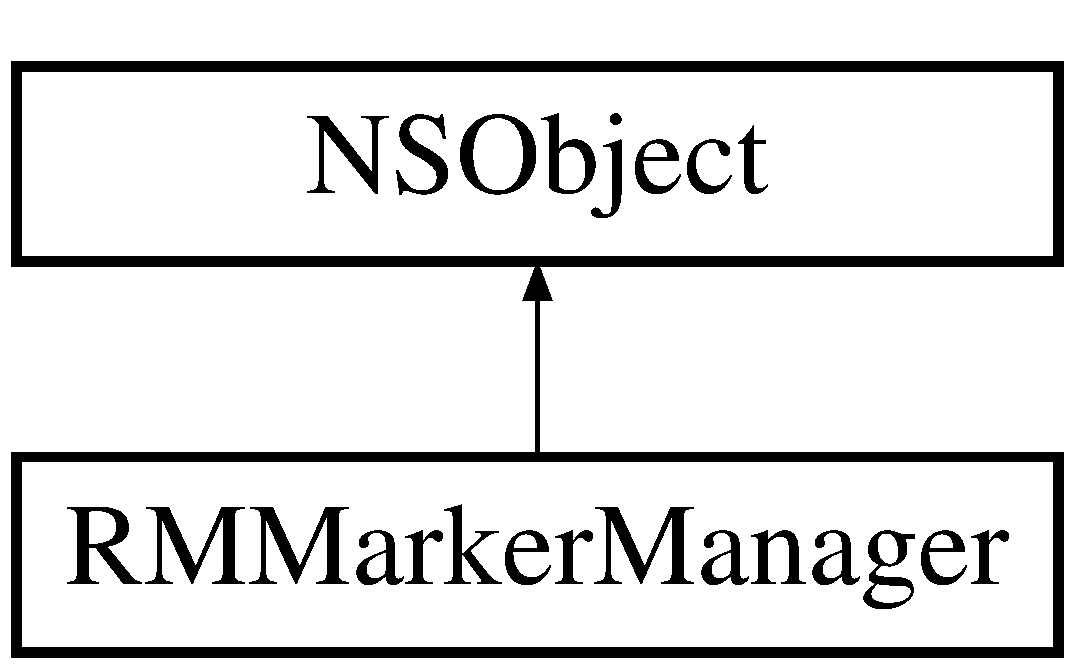
\includegraphics[height=2.000000cm]{interface_r_m_marker_manager}
\end{center}
\end{figure}
\subsection*{Instance Methods}
\begin{DoxyCompactItemize}
\item 
(void) -\/ \hyperlink{interface_r_m_marker_manager_aaa93d51f42410bfa5ffe089b9382bed5}{add\-Marker\-:\-At\-Lat\-Long\-:}
\begin{DoxyCompactList}\small\item\em place the (newly created) marker onto the map and take ownership of it \end{DoxyCompactList}\item 
(void) -\/ \hyperlink{interface_r_m_marker_manager_a76651ce7b6595adb6fec4a2454e34f22}{add\-Marker\-:at\-Projected\-Point\-:}
\begin{DoxyCompactList}\small\item\em place the (new created) marker onto the map at projected point and take ownership of it \end{DoxyCompactList}\item 
(void) -\/ \hyperlink{interface_r_m_marker_manager_a73a655d4e34dced726957ed025beb79b}{dealloc}{\ttfamily  \mbox{[}implementation\mbox{]}}
\item 
(void) -\/ \hyperlink{interface_r_m_marker_manager_ad3403a9206e18ced0f63afdc17645726}{hide\-All\-Markers}
\item 
(id) -\/ \hyperlink{interface_r_m_marker_manager_a3252cf457e206e61480c30874fe12c85}{init\-With\-Contents\-:}
\item 
(B\-O\-O\-L) -\/ \hyperlink{interface_r_m_marker_manager_a3460cd9600b65d6ec7f165382a1fc3f0}{is\-Marker\-:within\-Bounds\-:}
\item 
(B\-O\-O\-L) -\/ \hyperlink{interface_r_m_marker_manager_a17a9670fc21ae2a217371cabbf7158f1}{is\-Marker\-Within\-Screen\-Bounds\-:}
\item 
(C\-L\-Location\-Coordinate2\-D) -\/ \hyperlink{interface_r_m_marker_manager_a0caec53ea1bdf295feff4d2ee67c4d85}{latitude\-Longitude\-For\-Marker\-:}
\item 
(B\-O\-O\-L) -\/ \hyperlink{interface_r_m_marker_manager_aafee5503808e606438d714ad7a1ed55b}{managing\-Marker\-:}
\item 
(N\-S\-Array $\ast$) -\/ \hyperlink{interface_r_m_marker_manager_aa8076a5e1d59a93b3a7ee21b0cae63c1}{markers}
\item 
(N\-S\-Array $\ast$) -\/ \hyperlink{interface_r_m_marker_manager_a62301c581687b080ec2d66f7d740166c}{markers\-Within\-Screen\-Bounds}
\item 
(void) -\/ \hyperlink{interface_r_m_marker_manager_ac179d8f930721478732b25dc78fc6af8}{move\-Marker\-:\-At\-Lat\-Lon\-:}
\item 
(void) -\/ \hyperlink{interface_r_m_marker_manager_a1e774d2df5924a4632f61bd1565fe73a}{move\-Marker\-:\-At\-X\-Y\-:}
\item 
(void) -\/ \hyperlink{interface_r_m_marker_manager_a6f06af69ae8c4d41e114346df170e889}{remove\-Marker\-:}
\item 
(void) -\/ \hyperlink{interface_r_m_marker_manager_acc176d752af4381c94e357c7916707fc}{remove\-Markers}
\item 
(void) -\/ \hyperlink{interface_r_m_marker_manager_ace4f46970fea1660c61ed60c13741b4b}{remove\-Markers\-:}
\item 
(C\-G\-Point) -\/ \hyperlink{interface_r_m_marker_manager_a84726bc335efbd469bb7ac9da60f6641}{screen\-Coordinates\-For\-Marker\-:}
\item 
(void) -\/ \hyperlink{interface_r_m_marker_manager_ab6aa8d10dd932a782eb544d10dd9d3d1}{set\-Rotation\-:}
\item 
(void) -\/ \hyperlink{interface_r_m_marker_manager_ac31f5340920245dd9b6a3068c720fee1}{unhide\-All\-Markers}
\end{DoxyCompactItemize}
\subsection*{Protected 属性}
\begin{DoxyCompactItemize}
\item 
C\-G\-Affine\-Transform \hyperlink{interface_r_m_marker_manager_a1ad3a07eaa130021e43cf400a497e6d3}{rotation\-Transform}
\end{DoxyCompactItemize}
\subsection*{属性}
\begin{DoxyCompactItemize}
\item 
\hyperlink{interface_r_m_map_contents}{R\-M\-Map\-Contents} $\ast$ \hyperlink{interface_r_m_marker_manager_a5e24749c64023fbb7e2e3a161bb8f482}{contents}
\end{DoxyCompactItemize}


\subsection{Method Documentation}
\hypertarget{interface_r_m_marker_manager_aaa93d51f42410bfa5ffe089b9382bed5}{\index{R\-M\-Marker\-Manager@{R\-M\-Marker\-Manager}!add\-Marker\-:\-At\-Lat\-Long\-:@{add\-Marker\-:\-At\-Lat\-Long\-:}}
\index{add\-Marker\-:\-At\-Lat\-Long\-:@{add\-Marker\-:\-At\-Lat\-Long\-:}!RMMarkerManager@{R\-M\-Marker\-Manager}}
\subsubsection[{add\-Marker\-:\-At\-Lat\-Long\-:}]{\setlength{\rightskip}{0pt plus 5cm}-\/ (void) add\-Marker\-: 
\begin{DoxyParamCaption}
\item[{({\bf R\-M\-Marker}$\ast$)}]{marker}
\item[{AtLatLong:(C\-L\-Location\-Coordinate2\-D)}]{point}
\end{DoxyParamCaption}
}}\label{interface_r_m_marker_manager_aaa93d51f42410bfa5ffe089b9382bed5}


place the (newly created) marker onto the map and take ownership of it 

\begin{DoxyRefDesc}{Bug}
\item[\hyperlink{bug__bug000027}{Bug}]should return the marker \end{DoxyRefDesc}
\hypertarget{interface_r_m_marker_manager_a76651ce7b6595adb6fec4a2454e34f22}{\index{R\-M\-Marker\-Manager@{R\-M\-Marker\-Manager}!add\-Marker\-:at\-Projected\-Point\-:@{add\-Marker\-:at\-Projected\-Point\-:}}
\index{add\-Marker\-:at\-Projected\-Point\-:@{add\-Marker\-:at\-Projected\-Point\-:}!RMMarkerManager@{R\-M\-Marker\-Manager}}
\subsubsection[{add\-Marker\-:at\-Projected\-Point\-:}]{\setlength{\rightskip}{0pt plus 5cm}-\/ (void) add\-Marker\-: 
\begin{DoxyParamCaption}
\item[{({\bf R\-M\-Marker} $\ast$)}]{marker}
\item[{atProjectedPoint:({\bf R\-M\-Projected\-Point})}]{projected\-Point}
\end{DoxyParamCaption}
}}\label{interface_r_m_marker_manager_a76651ce7b6595adb6fec4a2454e34f22}


place the (new created) marker onto the map at projected point and take ownership of it 



参考自 add\-Marker\-:\-At\-Lat\-Long\-:.

\hypertarget{interface_r_m_marker_manager_a73a655d4e34dced726957ed025beb79b}{\index{R\-M\-Marker\-Manager@{R\-M\-Marker\-Manager}!dealloc@{dealloc}}
\index{dealloc@{dealloc}!RMMarkerManager@{R\-M\-Marker\-Manager}}
\subsubsection[{dealloc}]{\setlength{\rightskip}{0pt plus 5cm}-\/ (void) dealloc 
\begin{DoxyParamCaption}
{}
\end{DoxyParamCaption}
\hspace{0.3cm}{\ttfamily [implementation]}}}\label{interface_r_m_marker_manager_a73a655d4e34dced726957ed025beb79b}
\hypertarget{interface_r_m_marker_manager_ad3403a9206e18ced0f63afdc17645726}{\index{R\-M\-Marker\-Manager@{R\-M\-Marker\-Manager}!hide\-All\-Markers@{hide\-All\-Markers}}
\index{hide\-All\-Markers@{hide\-All\-Markers}!RMMarkerManager@{R\-M\-Marker\-Manager}}
\subsubsection[{hide\-All\-Markers}]{\setlength{\rightskip}{0pt plus 5cm}-\/ (void) hide\-All\-Markers 
\begin{DoxyParamCaption}
{}
\end{DoxyParamCaption}
}}\label{interface_r_m_marker_manager_ad3403a9206e18ced0f63afdc17645726}
\begin{DoxyRefDesc}{Bug}
\item[\hyperlink{bug__bug000029}{Bug}]this will hide path overlays too? \end{DoxyRefDesc}
\begin{DoxyRefDesc}{弃用}
\item[\hyperlink{deprecated__deprecated000011}{弃用}]syntactic sugar. Might have a place on \hyperlink{interface_r_m_map_view}{R\-M\-Map\-View}, but not on \hyperlink{interface_r_m_marker_manager}{R\-M\-Marker\-Manager}. \end{DoxyRefDesc}
\hypertarget{interface_r_m_marker_manager_a3252cf457e206e61480c30874fe12c85}{\index{R\-M\-Marker\-Manager@{R\-M\-Marker\-Manager}!init\-With\-Contents\-:@{init\-With\-Contents\-:}}
\index{init\-With\-Contents\-:@{init\-With\-Contents\-:}!RMMarkerManager@{R\-M\-Marker\-Manager}}
\subsubsection[{init\-With\-Contents\-:}]{\setlength{\rightskip}{0pt plus 5cm}-\/ (id) init\-With\-Contents\-: 
\begin{DoxyParamCaption}
\item[{({\bf R\-M\-Map\-Contents} $\ast$)}]{map\-Contents}
\end{DoxyParamCaption}
}}\label{interface_r_m_marker_manager_a3252cf457e206e61480c30874fe12c85}
\hypertarget{interface_r_m_marker_manager_a3460cd9600b65d6ec7f165382a1fc3f0}{\index{R\-M\-Marker\-Manager@{R\-M\-Marker\-Manager}!is\-Marker\-:within\-Bounds\-:@{is\-Marker\-:within\-Bounds\-:}}
\index{is\-Marker\-:within\-Bounds\-:@{is\-Marker\-:within\-Bounds\-:}!RMMarkerManager@{R\-M\-Marker\-Manager}}
\subsubsection[{is\-Marker\-:within\-Bounds\-:}]{\setlength{\rightskip}{0pt plus 5cm}-\/ (B\-O\-O\-L) is\-Marker\-: 
\begin{DoxyParamCaption}
\item[{({\bf R\-M\-Marker}$\ast$)}]{marker}
\item[{withinBounds:(C\-G\-Rect)}]{rect}
\end{DoxyParamCaption}
}}\label{interface_r_m_marker_manager_a3460cd9600b65d6ec7f165382a1fc3f0}
\begin{DoxyRefDesc}{弃用}
\item[\hyperlink{deprecated__deprecated000013}{弃用}]violates Objective-\/\-C naming rules \end{DoxyRefDesc}


参考自 is\-Marker\-Within\-Screen\-Bounds\-:.

\hypertarget{interface_r_m_marker_manager_a17a9670fc21ae2a217371cabbf7158f1}{\index{R\-M\-Marker\-Manager@{R\-M\-Marker\-Manager}!is\-Marker\-Within\-Screen\-Bounds\-:@{is\-Marker\-Within\-Screen\-Bounds\-:}}
\index{is\-Marker\-Within\-Screen\-Bounds\-:@{is\-Marker\-Within\-Screen\-Bounds\-:}!RMMarkerManager@{R\-M\-Marker\-Manager}}
\subsubsection[{is\-Marker\-Within\-Screen\-Bounds\-:}]{\setlength{\rightskip}{0pt plus 5cm}-\/ (B\-O\-O\-L) is\-Marker\-Within\-Screen\-Bounds\-: 
\begin{DoxyParamCaption}
\item[{({\bf R\-M\-Marker}$\ast$)}]{marker}
\end{DoxyParamCaption}
}}\label{interface_r_m_marker_manager_a17a9670fc21ae2a217371cabbf7158f1}
\hypertarget{interface_r_m_marker_manager_a0caec53ea1bdf295feff4d2ee67c4d85}{\index{R\-M\-Marker\-Manager@{R\-M\-Marker\-Manager}!latitude\-Longitude\-For\-Marker\-:@{latitude\-Longitude\-For\-Marker\-:}}
\index{latitude\-Longitude\-For\-Marker\-:@{latitude\-Longitude\-For\-Marker\-:}!RMMarkerManager@{R\-M\-Marker\-Manager}}
\subsubsection[{latitude\-Longitude\-For\-Marker\-:}]{\setlength{\rightskip}{0pt plus 5cm}-\/ (C\-L\-Location\-Coordinate2\-D) latitude\-Longitude\-For\-Marker\-: 
\begin{DoxyParamCaption}
\item[{({\bf R\-M\-Marker} $\ast$)}]{marker}
\end{DoxyParamCaption}
}}\label{interface_r_m_marker_manager_a0caec53ea1bdf295feff4d2ee67c4d85}


参考自 Route\-Me\-Tests\-::test\-Marker\-Coordinates\-Far\-East , 以及 Route\-Me\-Tests\-::test\-Marker\-Coordinates\-Far\-West.

\hypertarget{interface_r_m_marker_manager_aafee5503808e606438d714ad7a1ed55b}{\index{R\-M\-Marker\-Manager@{R\-M\-Marker\-Manager}!managing\-Marker\-:@{managing\-Marker\-:}}
\index{managing\-Marker\-:@{managing\-Marker\-:}!RMMarkerManager@{R\-M\-Marker\-Manager}}
\subsubsection[{managing\-Marker\-:}]{\setlength{\rightskip}{0pt plus 5cm}-\/ (B\-O\-O\-L) managing\-Marker\-: 
\begin{DoxyParamCaption}
\item[{({\bf R\-M\-Marker}$\ast$)}]{marker}
\end{DoxyParamCaption}
}}\label{interface_r_m_marker_manager_aafee5503808e606438d714ad7a1ed55b}
\begin{DoxyRefDesc}{弃用}
\item[\hyperlink{deprecated__deprecated000014}{弃用}]violates Objective-\/\-C naming rules \end{DoxyRefDesc}
\hypertarget{interface_r_m_marker_manager_aa8076a5e1d59a93b3a7ee21b0cae63c1}{\index{R\-M\-Marker\-Manager@{R\-M\-Marker\-Manager}!markers@{markers}}
\index{markers@{markers}!RMMarkerManager@{R\-M\-Marker\-Manager}}
\subsubsection[{markers}]{\setlength{\rightskip}{0pt plus 5cm}-\/ (N\-S\-Array $\ast$) markers 
\begin{DoxyParamCaption}
{}
\end{DoxyParamCaption}
}}\label{interface_r_m_marker_manager_aa8076a5e1d59a93b3a7ee21b0cae63c1}


参考自 managing\-Marker\-:, markers\-Within\-Screen\-Bounds , 以及 set\-Rotation\-:.

\hypertarget{interface_r_m_marker_manager_a62301c581687b080ec2d66f7d740166c}{\index{R\-M\-Marker\-Manager@{R\-M\-Marker\-Manager}!markers\-Within\-Screen\-Bounds@{markers\-Within\-Screen\-Bounds}}
\index{markers\-Within\-Screen\-Bounds@{markers\-Within\-Screen\-Bounds}!RMMarkerManager@{R\-M\-Marker\-Manager}}
\subsubsection[{markers\-Within\-Screen\-Bounds}]{\setlength{\rightskip}{0pt plus 5cm}-\/ (N\-S\-Array $\ast$) markers\-Within\-Screen\-Bounds 
\begin{DoxyParamCaption}
{}
\end{DoxyParamCaption}
}}\label{interface_r_m_marker_manager_a62301c581687b080ec2d66f7d740166c}
\hypertarget{interface_r_m_marker_manager_ac179d8f930721478732b25dc78fc6af8}{\index{R\-M\-Marker\-Manager@{R\-M\-Marker\-Manager}!move\-Marker\-:\-At\-Lat\-Lon\-:@{move\-Marker\-:\-At\-Lat\-Lon\-:}}
\index{move\-Marker\-:\-At\-Lat\-Lon\-:@{move\-Marker\-:\-At\-Lat\-Lon\-:}!RMMarkerManager@{R\-M\-Marker\-Manager}}
\subsubsection[{move\-Marker\-:\-At\-Lat\-Lon\-:}]{\setlength{\rightskip}{0pt plus 5cm}-\/ (void) move\-Marker\-: 
\begin{DoxyParamCaption}
\item[{({\bf R\-M\-Marker} $\ast$)}]{marker}
\item[{AtLatLon:({\bf R\-M\-Lat\-Long})}]{point}
\end{DoxyParamCaption}
}}\label{interface_r_m_marker_manager_ac179d8f930721478732b25dc78fc6af8}
\hypertarget{interface_r_m_marker_manager_a1e774d2df5924a4632f61bd1565fe73a}{\index{R\-M\-Marker\-Manager@{R\-M\-Marker\-Manager}!move\-Marker\-:\-At\-X\-Y\-:@{move\-Marker\-:\-At\-X\-Y\-:}}
\index{move\-Marker\-:\-At\-X\-Y\-:@{move\-Marker\-:\-At\-X\-Y\-:}!RMMarkerManager@{R\-M\-Marker\-Manager}}
\subsubsection[{move\-Marker\-:\-At\-X\-Y\-:}]{\setlength{\rightskip}{0pt plus 5cm}-\/ (void) move\-Marker\-: 
\begin{DoxyParamCaption}
\item[{({\bf R\-M\-Marker} $\ast$)}]{marker}
\item[{AtXY:(C\-G\-Point)}]{point}
\end{DoxyParamCaption}
}}\label{interface_r_m_marker_manager_a1e774d2df5924a4632f61bd1565fe73a}
\hypertarget{interface_r_m_marker_manager_a6f06af69ae8c4d41e114346df170e889}{\index{R\-M\-Marker\-Manager@{R\-M\-Marker\-Manager}!remove\-Marker\-:@{remove\-Marker\-:}}
\index{remove\-Marker\-:@{remove\-Marker\-:}!RMMarkerManager@{R\-M\-Marker\-Manager}}
\subsubsection[{remove\-Marker\-:}]{\setlength{\rightskip}{0pt plus 5cm}-\/ (void) remove\-Marker\-: 
\begin{DoxyParamCaption}
\item[{({\bf R\-M\-Marker} $\ast$)}]{marker}
\end{DoxyParamCaption}
}}\label{interface_r_m_marker_manager_a6f06af69ae8c4d41e114346df170e889}
\hypertarget{interface_r_m_marker_manager_acc176d752af4381c94e357c7916707fc}{\index{R\-M\-Marker\-Manager@{R\-M\-Marker\-Manager}!remove\-Markers@{remove\-Markers}}
\index{remove\-Markers@{remove\-Markers}!RMMarkerManager@{R\-M\-Marker\-Manager}}
\subsubsection[{remove\-Markers}]{\setlength{\rightskip}{0pt plus 5cm}-\/ (void) remove\-Markers 
\begin{DoxyParamCaption}
{}
\end{DoxyParamCaption}
}}\label{interface_r_m_marker_manager_acc176d752af4381c94e357c7916707fc}
\begin{DoxyRefDesc}{Bug}
\item[\hyperlink{bug__bug000028}{Bug}]see \href{http://code.google.com/p/route-me/issues/detail?id=75}{\tt http\-://code.\-google.\-com/p/route-\/me/issues/detail?id=75} (halmueller)\-: I am skeptical about interactions of this code with paths \end{DoxyRefDesc}
\hypertarget{interface_r_m_marker_manager_ace4f46970fea1660c61ed60c13741b4b}{\index{R\-M\-Marker\-Manager@{R\-M\-Marker\-Manager}!remove\-Markers\-:@{remove\-Markers\-:}}
\index{remove\-Markers\-:@{remove\-Markers\-:}!RMMarkerManager@{R\-M\-Marker\-Manager}}
\subsubsection[{remove\-Markers\-:}]{\setlength{\rightskip}{0pt plus 5cm}-\/ (void) remove\-Markers\-: 
\begin{DoxyParamCaption}
\item[{(N\-S\-Array $\ast$)}]{markers}
\end{DoxyParamCaption}
}}\label{interface_r_m_marker_manager_ace4f46970fea1660c61ed60c13741b4b}
\hypertarget{interface_r_m_marker_manager_a84726bc335efbd469bb7ac9da60f6641}{\index{R\-M\-Marker\-Manager@{R\-M\-Marker\-Manager}!screen\-Coordinates\-For\-Marker\-:@{screen\-Coordinates\-For\-Marker\-:}}
\index{screen\-Coordinates\-For\-Marker\-:@{screen\-Coordinates\-For\-Marker\-:}!RMMarkerManager@{R\-M\-Marker\-Manager}}
\subsubsection[{screen\-Coordinates\-For\-Marker\-:}]{\setlength{\rightskip}{0pt plus 5cm}-\/ (C\-G\-Point) screen\-Coordinates\-For\-Marker\-: 
\begin{DoxyParamCaption}
\item[{({\bf R\-M\-Marker} $\ast$)}]{marker}
\end{DoxyParamCaption}
}}\label{interface_r_m_marker_manager_a84726bc335efbd469bb7ac9da60f6641}


参考自 is\-Marker\-:within\-Bounds\-:, latitude\-Longitude\-For\-Marker\-:, Route\-Me\-Tests\-::test\-Marker\-Coordinates\-Far\-East , 以及 Route\-Me\-Tests\-::test\-Marker\-Coordinates\-Far\-West.

\hypertarget{interface_r_m_marker_manager_ab6aa8d10dd932a782eb544d10dd9d3d1}{\index{R\-M\-Marker\-Manager@{R\-M\-Marker\-Manager}!set\-Rotation\-:@{set\-Rotation\-:}}
\index{set\-Rotation\-:@{set\-Rotation\-:}!RMMarkerManager@{R\-M\-Marker\-Manager}}
\subsubsection[{set\-Rotation\-:}]{\setlength{\rightskip}{0pt plus 5cm}-\/ (void) set\-Rotation\-: 
\begin{DoxyParamCaption}
\item[{(float)}]{angle}
\end{DoxyParamCaption}
}}\label{interface_r_m_marker_manager_ab6aa8d10dd932a782eb544d10dd9d3d1}
\hypertarget{interface_r_m_marker_manager_ac31f5340920245dd9b6a3068c720fee1}{\index{R\-M\-Marker\-Manager@{R\-M\-Marker\-Manager}!unhide\-All\-Markers@{unhide\-All\-Markers}}
\index{unhide\-All\-Markers@{unhide\-All\-Markers}!RMMarkerManager@{R\-M\-Marker\-Manager}}
\subsubsection[{unhide\-All\-Markers}]{\setlength{\rightskip}{0pt plus 5cm}-\/ (void) unhide\-All\-Markers 
\begin{DoxyParamCaption}
{}
\end{DoxyParamCaption}
}}\label{interface_r_m_marker_manager_ac31f5340920245dd9b6a3068c720fee1}
\begin{DoxyRefDesc}{Bug}
\item[\hyperlink{bug__bug000030}{Bug}]this will hide path overlays too? \end{DoxyRefDesc}
\begin{DoxyRefDesc}{弃用}
\item[\hyperlink{deprecated__deprecated000012}{弃用}]syntactic sugar. Might have a place on \hyperlink{interface_r_m_map_view}{R\-M\-Map\-View}, but not on \hyperlink{interface_r_m_marker_manager}{R\-M\-Marker\-Manager}. \end{DoxyRefDesc}


\subsection{类成员变量说明}
\hypertarget{interface_r_m_marker_manager_a1ad3a07eaa130021e43cf400a497e6d3}{\index{R\-M\-Marker\-Manager@{R\-M\-Marker\-Manager}!rotation\-Transform@{rotation\-Transform}}
\index{rotation\-Transform@{rotation\-Transform}!RMMarkerManager@{R\-M\-Marker\-Manager}}
\subsubsection[{rotation\-Transform}]{\setlength{\rightskip}{0pt plus 5cm}-\/ (C\-G\-Affine\-Transform) rotation\-Transform\hspace{0.3cm}{\ttfamily [protected]}}}\label{interface_r_m_marker_manager_a1ad3a07eaa130021e43cf400a497e6d3}


参考自 init\-With\-Contents\-: , 以及 set\-Rotation\-:.



\subsection{属性说明}
\hypertarget{interface_r_m_marker_manager_a5e24749c64023fbb7e2e3a161bb8f482}{\index{R\-M\-Marker\-Manager@{R\-M\-Marker\-Manager}!contents@{contents}}
\index{contents@{contents}!RMMarkerManager@{R\-M\-Marker\-Manager}}
\subsubsection[{contents}]{\setlength{\rightskip}{0pt plus 5cm}-\/ ({\bf R\-M\-Map\-Contents} $\ast$) contents\hspace{0.3cm}{\ttfamily [read]}, {\ttfamily [write]}, {\ttfamily [atomic]}, {\ttfamily [assign]}}}\label{interface_r_m_marker_manager_a5e24749c64023fbb7e2e3a161bb8f482}


参考自 add\-Marker\-:\-At\-Lat\-Long\-:, add\-Marker\-:at\-Projected\-Point\-:, dealloc, hide\-All\-Markers, init\-With\-Contents\-:, is\-Marker\-Within\-Screen\-Bounds\-:, latitude\-Longitude\-For\-Marker\-:, markers, markers\-Within\-Screen\-Bounds, move\-Marker\-:\-At\-Lat\-Lon\-:, move\-Marker\-:\-At\-X\-Y\-:, remove\-Marker\-:, remove\-Markers, remove\-Markers\-:, screen\-Coordinates\-For\-Marker\-: , 以及 unhide\-All\-Markers.



该类的文档由以下文件生成\-:\begin{DoxyCompactItemize}
\item 
Map/\hyperlink{_r_m_marker_manager_8h}{R\-M\-Marker\-Manager.\-h}\item 
Map/\hyperlink{_r_m_marker_manager_8m}{R\-M\-Marker\-Manager.\-m}\end{DoxyCompactItemize}

\hypertarget{interface_r_m_m_b_tiles_tile_source}{\section{R\-M\-M\-B\-Tiles\-Tile\-Source类 参考}
\label{interface_r_m_m_b_tiles_tile_source}\index{R\-M\-M\-B\-Tiles\-Tile\-Source@{R\-M\-M\-B\-Tiles\-Tile\-Source}}
}


{\ttfamily \#import $<$R\-M\-M\-B\-Tiles\-Tile\-Source.\-h$>$}

类 R\-M\-M\-B\-Tiles\-Tile\-Source 继承关系图\-:\begin{figure}[H]
\begin{center}
\leavevmode
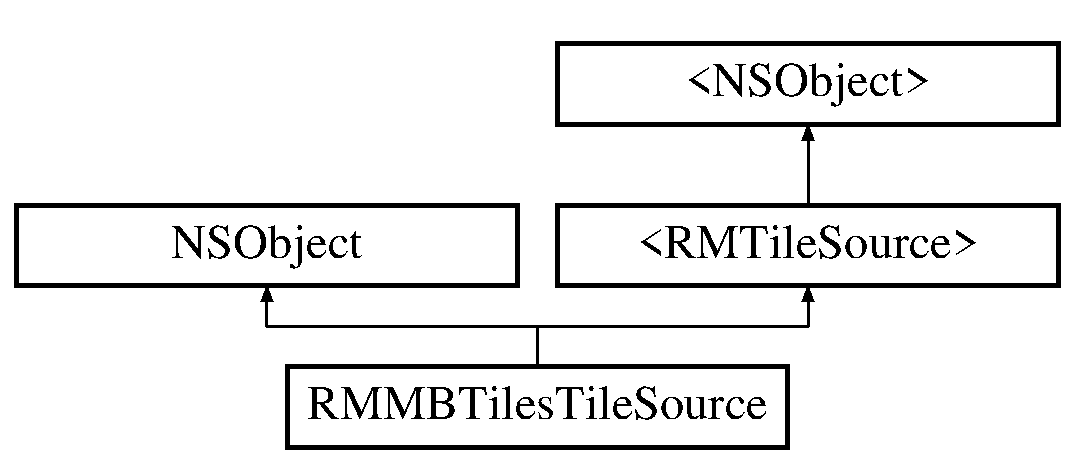
\includegraphics[height=3.000000cm]{interface_r_m_m_b_tiles_tile_source}
\end{center}
\end{figure}
\subsection*{Instance Methods}
\begin{DoxyCompactItemize}
\item 
(B\-O\-O\-L) -\/ \hyperlink{interface_r_m_m_b_tiles_tile_source_a79c6ebb930aed705a27b58c4d489d6d1}{covers\-Full\-World}
\item 
(void) -\/ \hyperlink{interface_r_m_m_b_tiles_tile_source_aea378c7d0d1c385bf5eeb8640f84bcb6}{dealloc}{\ttfamily  \mbox{[}implementation\mbox{]}}
\item 
(void) -\/ \hyperlink{interface_r_m_m_b_tiles_tile_source_a271c8c04b08b6cfb2a9f26cf4cf6b8fb}{did\-Receive\-Memory\-Warning}
\item 
(id) -\/ \hyperlink{interface_r_m_m_b_tiles_tile_source_a5440bebc2b66e5a49e0e74f2eddd4765}{init\-With\-Tile\-Set\-U\-R\-L\-:}
\item 
(\hyperlink{struct_r_m_spherical_trapezium}{R\-M\-Spherical\-Trapezium}) -\/ \hyperlink{interface_r_m_m_b_tiles_tile_source_a3916d8c4aa1c2a9943c9dcafcfb30b97}{latitude\-Longitude\-Bounding\-Box}
\item 
(\hyperlink{_r_m_m_b_tiles_tile_source_8h_a3ce7ea9300fb4b15a8031a62d1eef46c}{R\-M\-M\-B\-Tiles\-Layer\-Type}) -\/ \hyperlink{interface_r_m_m_b_tiles_tile_source_a8c6bc51a2878a1b462fa50004275f6bc}{layer\-Type}
\item 
(N\-S\-String $\ast$) -\/ \hyperlink{interface_r_m_m_b_tiles_tile_source_a8ec303f6909f461a5d33eb32e6f01a06}{legend}
\item 
(N\-S\-String $\ast$) -\/ \hyperlink{interface_r_m_m_b_tiles_tile_source_aedb3c1daf42a85b1037c719866ffabf7}{long\-Attribution}
\item 
(N\-S\-String $\ast$) -\/ \hyperlink{interface_r_m_m_b_tiles_tile_source_a437c5306c3918390b4ed9fda136c7b90}{long\-Description}
\item 
(float) -\/ \hyperlink{interface_r_m_m_b_tiles_tile_source_aeb23cf513462e0f3e907a7f3264009d9}{max\-Zoom}
\item 
(id$<$ \hyperlink{protocol_r_m_mercator_to_tile_projection-p}{R\-M\-Mercator\-To\-Tile\-Projection} $>$) -\/ \hyperlink{interface_r_m_m_b_tiles_tile_source_ab9abfb26588460e39c90eec6f0fe8758}{mercator\-To\-Tile\-Projection}
\item 
(float) -\/ \hyperlink{interface_r_m_m_b_tiles_tile_source_a8322d0c266bb2f26f1b3331f16f6a426}{min\-Zoom}
\item 
(\hyperlink{interface_r_m_projection}{R\-M\-Projection} $\ast$) -\/ \hyperlink{interface_r_m_m_b_tiles_tile_source_ae36211d298346afbebb04b8427023832}{projection}
\item 
(void) -\/ \hyperlink{interface_r_m_m_b_tiles_tile_source_aead47efbda8333a9fa3cf727b5843006}{remove\-All\-Cached\-Images}
\begin{DoxyCompactList}\small\item\em clear all images from the in-\/memory and on-\/disk image caches \end{DoxyCompactList}\item 
(void) -\/ \hyperlink{interface_r_m_m_b_tiles_tile_source_a031f0f9ff2eff5dc0d65baa06da2a167}{set\-Max\-Zoom\-:}
\item 
(void) -\/ \hyperlink{interface_r_m_m_b_tiles_tile_source_a9f061bba0392cbeba80d32d22b750c39}{set\-Min\-Zoom\-:}
\item 
(void) -\/ \hyperlink{interface_r_m_m_b_tiles_tile_source_a0eff5e1c822a2c039ab9cce43d337d6b}{set\-Tile\-Side\-Length\-:}
\item 
(N\-S\-String $\ast$) -\/ \hyperlink{interface_r_m_m_b_tiles_tile_source_a82fceefd32c5831a55e036b758d0e1f8}{short\-Attribution}
\item 
(N\-S\-String $\ast$) -\/ \hyperlink{interface_r_m_m_b_tiles_tile_source_ad8675324133d0b2db398d5eaf52b62a1}{short\-Name}
\item 
(N\-S\-String $\ast$) -\/ \hyperlink{interface_r_m_m_b_tiles_tile_source_a52857f152e182aa84b545c0b92e8cc92}{tile\-File\-:}
\item 
(\hyperlink{interface_r_m_tile_image}{R\-M\-Tile\-Image} $\ast$) -\/ \hyperlink{interface_r_m_m_b_tiles_tile_source_a4328f717c85aed3131d957616bb2c0de}{tile\-Image\-:}
\item 
(N\-S\-String $\ast$) -\/ \hyperlink{interface_r_m_m_b_tiles_tile_source_a74b694ffc620b97720509cbb0b3b2fdc}{tile\-Path}
\item 
(int) -\/ \hyperlink{interface_r_m_m_b_tiles_tile_source_a064b2c04e404680e4e7d5ad82fca48e8}{tile\-Side\-Length}
\item 
(N\-S\-String $\ast$) -\/ \hyperlink{interface_r_m_m_b_tiles_tile_source_aa200e9b52ab97d586d712177d31ac13f}{tile\-U\-R\-L\-:}
\item 
(N\-S\-String $\ast$) -\/ \hyperlink{interface_r_m_m_b_tiles_tile_source_ab71dd47e8661b24cb264932e78b666a6}{unique\-Tilecache\-Key}
\end{DoxyCompactItemize}
\subsection*{Protected 属性}
\begin{DoxyCompactItemize}
\item 
F\-M\-Database $\ast$ \hyperlink{interface_r_m_m_b_tiles_tile_source_ae3da662873347f8608f9d6dc3b450771}{db}
\item 
\hyperlink{interface_r_m_fractal_tile_projection}{R\-M\-Fractal\-Tile\-Projection} $\ast$ \hyperlink{interface_r_m_m_b_tiles_tile_source_a3daa7aaad56a256e9feef893221306be}{tile\-Projection}
\end{DoxyCompactItemize}


\subsection{Method Documentation}
\hypertarget{interface_r_m_m_b_tiles_tile_source_a79c6ebb930aed705a27b58c4d489d6d1}{\index{R\-M\-M\-B\-Tiles\-Tile\-Source@{R\-M\-M\-B\-Tiles\-Tile\-Source}!covers\-Full\-World@{covers\-Full\-World}}
\index{covers\-Full\-World@{covers\-Full\-World}!RMMBTilesTileSource@{R\-M\-M\-B\-Tiles\-Tile\-Source}}
\subsubsection[{covers\-Full\-World}]{\setlength{\rightskip}{0pt plus 5cm}-\/ (B\-O\-O\-L) covers\-Full\-World 
\begin{DoxyParamCaption}
{}
\end{DoxyParamCaption}
}}\label{interface_r_m_m_b_tiles_tile_source_a79c6ebb930aed705a27b58c4d489d6d1}
\hypertarget{interface_r_m_m_b_tiles_tile_source_aea378c7d0d1c385bf5eeb8640f84bcb6}{\index{R\-M\-M\-B\-Tiles\-Tile\-Source@{R\-M\-M\-B\-Tiles\-Tile\-Source}!dealloc@{dealloc}}
\index{dealloc@{dealloc}!RMMBTilesTileSource@{R\-M\-M\-B\-Tiles\-Tile\-Source}}
\subsubsection[{dealloc}]{\setlength{\rightskip}{0pt plus 5cm}-\/ (void) dealloc 
\begin{DoxyParamCaption}
{}
\end{DoxyParamCaption}
\hspace{0.3cm}{\ttfamily [implementation]}}}\label{interface_r_m_m_b_tiles_tile_source_aea378c7d0d1c385bf5eeb8640f84bcb6}
\hypertarget{interface_r_m_m_b_tiles_tile_source_a271c8c04b08b6cfb2a9f26cf4cf6b8fb}{\index{R\-M\-M\-B\-Tiles\-Tile\-Source@{R\-M\-M\-B\-Tiles\-Tile\-Source}!did\-Receive\-Memory\-Warning@{did\-Receive\-Memory\-Warning}}
\index{did\-Receive\-Memory\-Warning@{did\-Receive\-Memory\-Warning}!RMMBTilesTileSource@{R\-M\-M\-B\-Tiles\-Tile\-Source}}
\subsubsection[{did\-Receive\-Memory\-Warning}]{\setlength{\rightskip}{0pt plus 5cm}-\/ (void) did\-Receive\-Memory\-Warning 
\begin{DoxyParamCaption}
{}
\end{DoxyParamCaption}
}}\label{interface_r_m_m_b_tiles_tile_source_a271c8c04b08b6cfb2a9f26cf4cf6b8fb}


重载 \hyperlink{protocol_r_m_tile_source-p_a70eade96883de23124c3f86321685b52}{$<$\-R\-M\-Tile\-Source$>$} .

\hypertarget{interface_r_m_m_b_tiles_tile_source_a5440bebc2b66e5a49e0e74f2eddd4765}{\index{R\-M\-M\-B\-Tiles\-Tile\-Source@{R\-M\-M\-B\-Tiles\-Tile\-Source}!init\-With\-Tile\-Set\-U\-R\-L\-:@{init\-With\-Tile\-Set\-U\-R\-L\-:}}
\index{init\-With\-Tile\-Set\-U\-R\-L\-:@{init\-With\-Tile\-Set\-U\-R\-L\-:}!RMMBTilesTileSource@{R\-M\-M\-B\-Tiles\-Tile\-Source}}
\subsubsection[{init\-With\-Tile\-Set\-U\-R\-L\-:}]{\setlength{\rightskip}{0pt plus 5cm}-\/ (id) init\-With\-Tile\-Set\-U\-R\-L\-: 
\begin{DoxyParamCaption}
\item[{(N\-S\-U\-R\-L $\ast$)}]{tile\-Set\-U\-R\-L}
\end{DoxyParamCaption}
}}\label{interface_r_m_m_b_tiles_tile_source_a5440bebc2b66e5a49e0e74f2eddd4765}
\hypertarget{interface_r_m_m_b_tiles_tile_source_a3916d8c4aa1c2a9943c9dcafcfb30b97}{\index{R\-M\-M\-B\-Tiles\-Tile\-Source@{R\-M\-M\-B\-Tiles\-Tile\-Source}!latitude\-Longitude\-Bounding\-Box@{latitude\-Longitude\-Bounding\-Box}}
\index{latitude\-Longitude\-Bounding\-Box@{latitude\-Longitude\-Bounding\-Box}!RMMBTilesTileSource@{R\-M\-M\-B\-Tiles\-Tile\-Source}}
\subsubsection[{latitude\-Longitude\-Bounding\-Box}]{\setlength{\rightskip}{0pt plus 5cm}-\/ ({\bf R\-M\-Spherical\-Trapezium}) latitude\-Longitude\-Bounding\-Box 
\begin{DoxyParamCaption}
{}
\end{DoxyParamCaption}
}}\label{interface_r_m_m_b_tiles_tile_source_a3916d8c4aa1c2a9943c9dcafcfb30b97}


重载 \hyperlink{protocol_r_m_tile_source-p_a740893daebd1fe8e0a463e64a28816dd}{$<$\-R\-M\-Tile\-Source$>$} .



参考自 covers\-Full\-World.

\hypertarget{interface_r_m_m_b_tiles_tile_source_a8c6bc51a2878a1b462fa50004275f6bc}{\index{R\-M\-M\-B\-Tiles\-Tile\-Source@{R\-M\-M\-B\-Tiles\-Tile\-Source}!layer\-Type@{layer\-Type}}
\index{layer\-Type@{layer\-Type}!RMMBTilesTileSource@{R\-M\-M\-B\-Tiles\-Tile\-Source}}
\subsubsection[{layer\-Type}]{\setlength{\rightskip}{0pt plus 5cm}-\/ ({\bf R\-M\-M\-B\-Tiles\-Layer\-Type}) layer\-Type 
\begin{DoxyParamCaption}
{}
\end{DoxyParamCaption}
}}\label{interface_r_m_m_b_tiles_tile_source_a8c6bc51a2878a1b462fa50004275f6bc}
\hypertarget{interface_r_m_m_b_tiles_tile_source_a8ec303f6909f461a5d33eb32e6f01a06}{\index{R\-M\-M\-B\-Tiles\-Tile\-Source@{R\-M\-M\-B\-Tiles\-Tile\-Source}!legend@{legend}}
\index{legend@{legend}!RMMBTilesTileSource@{R\-M\-M\-B\-Tiles\-Tile\-Source}}
\subsubsection[{legend}]{\setlength{\rightskip}{0pt plus 5cm}-\/ (N\-S\-String $\ast$) legend 
\begin{DoxyParamCaption}
{}
\end{DoxyParamCaption}
}}\label{interface_r_m_m_b_tiles_tile_source_a8ec303f6909f461a5d33eb32e6f01a06}
\hypertarget{interface_r_m_m_b_tiles_tile_source_aedb3c1daf42a85b1037c719866ffabf7}{\index{R\-M\-M\-B\-Tiles\-Tile\-Source@{R\-M\-M\-B\-Tiles\-Tile\-Source}!long\-Attribution@{long\-Attribution}}
\index{long\-Attribution@{long\-Attribution}!RMMBTilesTileSource@{R\-M\-M\-B\-Tiles\-Tile\-Source}}
\subsubsection[{long\-Attribution}]{\setlength{\rightskip}{0pt plus 5cm}-\/ (N\-S\-String $\ast$) long\-Attribution 
\begin{DoxyParamCaption}
{}
\end{DoxyParamCaption}
}}\label{interface_r_m_m_b_tiles_tile_source_aedb3c1daf42a85b1037c719866ffabf7}


重载 \hyperlink{protocol_r_m_tile_source-p_adff372c4c777906e56b90a61895d2ff4}{$<$\-R\-M\-Tile\-Source$>$} .

\hypertarget{interface_r_m_m_b_tiles_tile_source_a437c5306c3918390b4ed9fda136c7b90}{\index{R\-M\-M\-B\-Tiles\-Tile\-Source@{R\-M\-M\-B\-Tiles\-Tile\-Source}!long\-Description@{long\-Description}}
\index{long\-Description@{long\-Description}!RMMBTilesTileSource@{R\-M\-M\-B\-Tiles\-Tile\-Source}}
\subsubsection[{long\-Description}]{\setlength{\rightskip}{0pt plus 5cm}-\/ (N\-S\-String $\ast$) long\-Description 
\begin{DoxyParamCaption}
{}
\end{DoxyParamCaption}
}}\label{interface_r_m_m_b_tiles_tile_source_a437c5306c3918390b4ed9fda136c7b90}


重载 \hyperlink{protocol_r_m_tile_source-p_a1f9b03c3dac588a98b050afe3a71dcfa}{$<$\-R\-M\-Tile\-Source$>$} .

\hypertarget{interface_r_m_m_b_tiles_tile_source_aeb23cf513462e0f3e907a7f3264009d9}{\index{R\-M\-M\-B\-Tiles\-Tile\-Source@{R\-M\-M\-B\-Tiles\-Tile\-Source}!max\-Zoom@{max\-Zoom}}
\index{max\-Zoom@{max\-Zoom}!RMMBTilesTileSource@{R\-M\-M\-B\-Tiles\-Tile\-Source}}
\subsubsection[{max\-Zoom}]{\setlength{\rightskip}{0pt plus 5cm}-\/ (float) max\-Zoom 
\begin{DoxyParamCaption}
{}
\end{DoxyParamCaption}
}}\label{interface_r_m_m_b_tiles_tile_source_aeb23cf513462e0f3e907a7f3264009d9}


重载 \hyperlink{protocol_r_m_tile_source-p_a7d1ecfedd45c8ac433f972f38e7ac9a4}{$<$\-R\-M\-Tile\-Source$>$} .

\hypertarget{interface_r_m_m_b_tiles_tile_source_ab9abfb26588460e39c90eec6f0fe8758}{\index{R\-M\-M\-B\-Tiles\-Tile\-Source@{R\-M\-M\-B\-Tiles\-Tile\-Source}!mercator\-To\-Tile\-Projection@{mercator\-To\-Tile\-Projection}}
\index{mercator\-To\-Tile\-Projection@{mercator\-To\-Tile\-Projection}!RMMBTilesTileSource@{R\-M\-M\-B\-Tiles\-Tile\-Source}}
\subsubsection[{mercator\-To\-Tile\-Projection}]{\setlength{\rightskip}{0pt plus 5cm}-\/ (id$<$ {\bf R\-M\-Mercator\-To\-Tile\-Projection} $>$) mercator\-To\-Tile\-Projection 
\begin{DoxyParamCaption}
{}
\end{DoxyParamCaption}
}}\label{interface_r_m_m_b_tiles_tile_source_ab9abfb26588460e39c90eec6f0fe8758}


重载 \hyperlink{protocol_r_m_tile_source-p_a5086edf762a1756058c665c3a9b0d26f}{$<$\-R\-M\-Tile\-Source$>$} .

\hypertarget{interface_r_m_m_b_tiles_tile_source_a8322d0c266bb2f26f1b3331f16f6a426}{\index{R\-M\-M\-B\-Tiles\-Tile\-Source@{R\-M\-M\-B\-Tiles\-Tile\-Source}!min\-Zoom@{min\-Zoom}}
\index{min\-Zoom@{min\-Zoom}!RMMBTilesTileSource@{R\-M\-M\-B\-Tiles\-Tile\-Source}}
\subsubsection[{min\-Zoom}]{\setlength{\rightskip}{0pt plus 5cm}-\/ (float) min\-Zoom 
\begin{DoxyParamCaption}
{}
\end{DoxyParamCaption}
}}\label{interface_r_m_m_b_tiles_tile_source_a8322d0c266bb2f26f1b3331f16f6a426}


重载 \hyperlink{protocol_r_m_tile_source-p_a7cd043d2bc55eded244b4c5da41dd909}{$<$\-R\-M\-Tile\-Source$>$} .

\hypertarget{interface_r_m_m_b_tiles_tile_source_ae36211d298346afbebb04b8427023832}{\index{R\-M\-M\-B\-Tiles\-Tile\-Source@{R\-M\-M\-B\-Tiles\-Tile\-Source}!projection@{projection}}
\index{projection@{projection}!RMMBTilesTileSource@{R\-M\-M\-B\-Tiles\-Tile\-Source}}
\subsubsection[{projection}]{\setlength{\rightskip}{0pt plus 5cm}-\/ ({\bf R\-M\-Projection} $\ast$) projection 
\begin{DoxyParamCaption}
{}
\end{DoxyParamCaption}
}}\label{interface_r_m_m_b_tiles_tile_source_ae36211d298346afbebb04b8427023832}


重载 \hyperlink{protocol_r_m_tile_source-p_a75c20205e72db39aa01943d8b6d8fc29}{$<$\-R\-M\-Tile\-Source$>$} .



参考自 init\-With\-Tile\-Set\-U\-R\-L\-:.

\hypertarget{interface_r_m_m_b_tiles_tile_source_aead47efbda8333a9fa3cf727b5843006}{\index{R\-M\-M\-B\-Tiles\-Tile\-Source@{R\-M\-M\-B\-Tiles\-Tile\-Source}!remove\-All\-Cached\-Images@{remove\-All\-Cached\-Images}}
\index{remove\-All\-Cached\-Images@{remove\-All\-Cached\-Images}!RMMBTilesTileSource@{R\-M\-M\-B\-Tiles\-Tile\-Source}}
\subsubsection[{remove\-All\-Cached\-Images}]{\setlength{\rightskip}{0pt plus 5cm}-\/ (void) remove\-All\-Cached\-Images 
\begin{DoxyParamCaption}
{}
\end{DoxyParamCaption}
}}\label{interface_r_m_m_b_tiles_tile_source_aead47efbda8333a9fa3cf727b5843006}


clear all images from the in-\/memory and on-\/disk image caches 

\begin{DoxyRefDesc}{Bug}
\item[\hyperlink{bug__bug000052}{Bug}]This method belongs on \hyperlink{interface_r_m_cached_tile_source}{R\-M\-Cached\-Tile\-Source}, not on \hyperlink{protocol_r_m_tile_source-p}{R\-M\-Tile\-Source}, because an \hyperlink{protocol_r_m_tile_source-p}{R\-M\-Tile\-Source} doesn't have a cache. \end{DoxyRefDesc}


重载 \hyperlink{protocol_r_m_tile_source-p_aa5c4555fb2500e5826d5558985d4ee3c}{$<$\-R\-M\-Tile\-Source$>$} .

\hypertarget{interface_r_m_m_b_tiles_tile_source_a031f0f9ff2eff5dc0d65baa06da2a167}{\index{R\-M\-M\-B\-Tiles\-Tile\-Source@{R\-M\-M\-B\-Tiles\-Tile\-Source}!set\-Max\-Zoom\-:@{set\-Max\-Zoom\-:}}
\index{set\-Max\-Zoom\-:@{set\-Max\-Zoom\-:}!RMMBTilesTileSource@{R\-M\-M\-B\-Tiles\-Tile\-Source}}
\subsubsection[{set\-Max\-Zoom\-:}]{\setlength{\rightskip}{0pt plus 5cm}-\/ (void) set\-Max\-Zoom\-: 
\begin{DoxyParamCaption}
\item[{(N\-S\-U\-Integer)}]{a\-Max\-Zoom}
\end{DoxyParamCaption}
}}\label{interface_r_m_m_b_tiles_tile_source_a031f0f9ff2eff5dc0d65baa06da2a167}


重载 \hyperlink{protocol_r_m_tile_source-p_afd2310f2b3b95e91de2ef530ee5d5122}{$<$\-R\-M\-Tile\-Source$>$} .

\hypertarget{interface_r_m_m_b_tiles_tile_source_a9f061bba0392cbeba80d32d22b750c39}{\index{R\-M\-M\-B\-Tiles\-Tile\-Source@{R\-M\-M\-B\-Tiles\-Tile\-Source}!set\-Min\-Zoom\-:@{set\-Min\-Zoom\-:}}
\index{set\-Min\-Zoom\-:@{set\-Min\-Zoom\-:}!RMMBTilesTileSource@{R\-M\-M\-B\-Tiles\-Tile\-Source}}
\subsubsection[{set\-Min\-Zoom\-:}]{\setlength{\rightskip}{0pt plus 5cm}-\/ (void) set\-Min\-Zoom\-: 
\begin{DoxyParamCaption}
\item[{(N\-S\-U\-Integer)}]{a\-Min\-Zoom}
\end{DoxyParamCaption}
}}\label{interface_r_m_m_b_tiles_tile_source_a9f061bba0392cbeba80d32d22b750c39}


重载 \hyperlink{protocol_r_m_tile_source-p_ad8b2d3ab319784223970f215f6dd2f16}{$<$\-R\-M\-Tile\-Source$>$} .

\hypertarget{interface_r_m_m_b_tiles_tile_source_a0eff5e1c822a2c039ab9cce43d337d6b}{\index{R\-M\-M\-B\-Tiles\-Tile\-Source@{R\-M\-M\-B\-Tiles\-Tile\-Source}!set\-Tile\-Side\-Length\-:@{set\-Tile\-Side\-Length\-:}}
\index{set\-Tile\-Side\-Length\-:@{set\-Tile\-Side\-Length\-:}!RMMBTilesTileSource@{R\-M\-M\-B\-Tiles\-Tile\-Source}}
\subsubsection[{set\-Tile\-Side\-Length\-:}]{\setlength{\rightskip}{0pt plus 5cm}-\/ (void) set\-Tile\-Side\-Length\-: 
\begin{DoxyParamCaption}
\item[{(N\-S\-U\-Integer)}]{a\-Tile\-Side\-Length}
\end{DoxyParamCaption}
}}\label{interface_r_m_m_b_tiles_tile_source_a0eff5e1c822a2c039ab9cce43d337d6b}
\hypertarget{interface_r_m_m_b_tiles_tile_source_a82fceefd32c5831a55e036b758d0e1f8}{\index{R\-M\-M\-B\-Tiles\-Tile\-Source@{R\-M\-M\-B\-Tiles\-Tile\-Source}!short\-Attribution@{short\-Attribution}}
\index{short\-Attribution@{short\-Attribution}!RMMBTilesTileSource@{R\-M\-M\-B\-Tiles\-Tile\-Source}}
\subsubsection[{short\-Attribution}]{\setlength{\rightskip}{0pt plus 5cm}-\/ (N\-S\-String $\ast$) short\-Attribution 
\begin{DoxyParamCaption}
{}
\end{DoxyParamCaption}
}}\label{interface_r_m_m_b_tiles_tile_source_a82fceefd32c5831a55e036b758d0e1f8}


重载 \hyperlink{protocol_r_m_tile_source-p_afd67cfacb812cd3216ef1309297e264d}{$<$\-R\-M\-Tile\-Source$>$} .



参考自 long\-Attribution.

\hypertarget{interface_r_m_m_b_tiles_tile_source_ad8675324133d0b2db398d5eaf52b62a1}{\index{R\-M\-M\-B\-Tiles\-Tile\-Source@{R\-M\-M\-B\-Tiles\-Tile\-Source}!short\-Name@{short\-Name}}
\index{short\-Name@{short\-Name}!RMMBTilesTileSource@{R\-M\-M\-B\-Tiles\-Tile\-Source}}
\subsubsection[{short\-Name}]{\setlength{\rightskip}{0pt plus 5cm}-\/ (N\-S\-String $\ast$) short\-Name 
\begin{DoxyParamCaption}
{}
\end{DoxyParamCaption}
}}\label{interface_r_m_m_b_tiles_tile_source_ad8675324133d0b2db398d5eaf52b62a1}


重载 \hyperlink{protocol_r_m_tile_source-p_ae0a98ebf46579f4c29d434322d25e64e}{$<$\-R\-M\-Tile\-Source$>$} .



参考自 long\-Attribution , 以及 long\-Description.

\hypertarget{interface_r_m_m_b_tiles_tile_source_a52857f152e182aa84b545c0b92e8cc92}{\index{R\-M\-M\-B\-Tiles\-Tile\-Source@{R\-M\-M\-B\-Tiles\-Tile\-Source}!tile\-File\-:@{tile\-File\-:}}
\index{tile\-File\-:@{tile\-File\-:}!RMMBTilesTileSource@{R\-M\-M\-B\-Tiles\-Tile\-Source}}
\subsubsection[{tile\-File\-:}]{\setlength{\rightskip}{0pt plus 5cm}-\/ (N\-S\-String $\ast$) tile\-File\-: 
\begin{DoxyParamCaption}
\item[{({\bf R\-M\-Tile})}]{tile}
\end{DoxyParamCaption}
}}\label{interface_r_m_m_b_tiles_tile_source_a52857f152e182aa84b545c0b92e8cc92}


重载 \hyperlink{protocol_r_m_tile_source-p_adc40bd2f04352819fc05e32d4209a2ca}{$<$\-R\-M\-Tile\-Source$>$} .

\hypertarget{interface_r_m_m_b_tiles_tile_source_a4328f717c85aed3131d957616bb2c0de}{\index{R\-M\-M\-B\-Tiles\-Tile\-Source@{R\-M\-M\-B\-Tiles\-Tile\-Source}!tile\-Image\-:@{tile\-Image\-:}}
\index{tile\-Image\-:@{tile\-Image\-:}!RMMBTilesTileSource@{R\-M\-M\-B\-Tiles\-Tile\-Source}}
\subsubsection[{tile\-Image\-:}]{\setlength{\rightskip}{0pt plus 5cm}-\/ ({\bf R\-M\-Tile\-Image} $\ast$) tile\-Image\-: 
\begin{DoxyParamCaption}
\item[{({\bf R\-M\-Tile})}]{tile}
\end{DoxyParamCaption}
}}\label{interface_r_m_m_b_tiles_tile_source_a4328f717c85aed3131d957616bb2c0de}


重载 \hyperlink{protocol_r_m_tile_source-p_acf4ee01e3c1606d46a2ec8fe52b0d029}{$<$\-R\-M\-Tile\-Source$>$} .

\hypertarget{interface_r_m_m_b_tiles_tile_source_a74b694ffc620b97720509cbb0b3b2fdc}{\index{R\-M\-M\-B\-Tiles\-Tile\-Source@{R\-M\-M\-B\-Tiles\-Tile\-Source}!tile\-Path@{tile\-Path}}
\index{tile\-Path@{tile\-Path}!RMMBTilesTileSource@{R\-M\-M\-B\-Tiles\-Tile\-Source}}
\subsubsection[{tile\-Path}]{\setlength{\rightskip}{0pt plus 5cm}-\/ (N\-S\-String $\ast$) tile\-Path 
\begin{DoxyParamCaption}
{}
\end{DoxyParamCaption}
}}\label{interface_r_m_m_b_tiles_tile_source_a74b694ffc620b97720509cbb0b3b2fdc}


重载 \hyperlink{protocol_r_m_tile_source-p_ae9fc8d2cccf8a7ffce2a0f7837140b9b}{$<$\-R\-M\-Tile\-Source$>$} .

\hypertarget{interface_r_m_m_b_tiles_tile_source_a064b2c04e404680e4e7d5ad82fca48e8}{\index{R\-M\-M\-B\-Tiles\-Tile\-Source@{R\-M\-M\-B\-Tiles\-Tile\-Source}!tile\-Side\-Length@{tile\-Side\-Length}}
\index{tile\-Side\-Length@{tile\-Side\-Length}!RMMBTilesTileSource@{R\-M\-M\-B\-Tiles\-Tile\-Source}}
\subsubsection[{tile\-Side\-Length}]{\setlength{\rightskip}{0pt plus 5cm}-\/ (int) tile\-Side\-Length 
\begin{DoxyParamCaption}
{}
\end{DoxyParamCaption}
}}\label{interface_r_m_m_b_tiles_tile_source_a064b2c04e404680e4e7d5ad82fca48e8}
\hypertarget{interface_r_m_m_b_tiles_tile_source_aa200e9b52ab97d586d712177d31ac13f}{\index{R\-M\-M\-B\-Tiles\-Tile\-Source@{R\-M\-M\-B\-Tiles\-Tile\-Source}!tile\-U\-R\-L\-:@{tile\-U\-R\-L\-:}}
\index{tile\-U\-R\-L\-:@{tile\-U\-R\-L\-:}!RMMBTilesTileSource@{R\-M\-M\-B\-Tiles\-Tile\-Source}}
\subsubsection[{tile\-U\-R\-L\-:}]{\setlength{\rightskip}{0pt plus 5cm}-\/ (N\-S\-String $\ast$) tile\-U\-R\-L\-: 
\begin{DoxyParamCaption}
\item[{({\bf R\-M\-Tile})}]{tile}
\end{DoxyParamCaption}
}}\label{interface_r_m_m_b_tiles_tile_source_aa200e9b52ab97d586d712177d31ac13f}


重载 \hyperlink{protocol_r_m_tile_source-p_af7ca2e2fb8e8cc4cb17433ffdc105230}{$<$\-R\-M\-Tile\-Source$>$} .

\hypertarget{interface_r_m_m_b_tiles_tile_source_ab71dd47e8661b24cb264932e78b666a6}{\index{R\-M\-M\-B\-Tiles\-Tile\-Source@{R\-M\-M\-B\-Tiles\-Tile\-Source}!unique\-Tilecache\-Key@{unique\-Tilecache\-Key}}
\index{unique\-Tilecache\-Key@{unique\-Tilecache\-Key}!RMMBTilesTileSource@{R\-M\-M\-B\-Tiles\-Tile\-Source}}
\subsubsection[{unique\-Tilecache\-Key}]{\setlength{\rightskip}{0pt plus 5cm}-\/ (N\-S\-String $\ast$) unique\-Tilecache\-Key 
\begin{DoxyParamCaption}
{}
\end{DoxyParamCaption}
}}\label{interface_r_m_m_b_tiles_tile_source_ab71dd47e8661b24cb264932e78b666a6}


重载 \hyperlink{protocol_r_m_tile_source-p_a1838a34e9341efe7c76252e131824261}{$<$\-R\-M\-Tile\-Source$>$} .



\subsection{类成员变量说明}
\hypertarget{interface_r_m_m_b_tiles_tile_source_ae3da662873347f8608f9d6dc3b450771}{\index{R\-M\-M\-B\-Tiles\-Tile\-Source@{R\-M\-M\-B\-Tiles\-Tile\-Source}!db@{db}}
\index{db@{db}!RMMBTilesTileSource@{R\-M\-M\-B\-Tiles\-Tile\-Source}}
\subsubsection[{db}]{\setlength{\rightskip}{0pt plus 5cm}-\/ (F\-M\-Database$\ast$) db\hspace{0.3cm}{\ttfamily [protected]}}}\label{interface_r_m_m_b_tiles_tile_source_ae3da662873347f8608f9d6dc3b450771}


参考自 dealloc, init\-With\-Tile\-Set\-U\-R\-L\-:, latitude\-Longitude\-Bounding\-Box, layer\-Type, legend, long\-Description, max\-Zoom, min\-Zoom, short\-Attribution, short\-Name, tile\-Image\-: , 以及 unique\-Tilecache\-Key.

\hypertarget{interface_r_m_m_b_tiles_tile_source_a3daa7aaad56a256e9feef893221306be}{\index{R\-M\-M\-B\-Tiles\-Tile\-Source@{R\-M\-M\-B\-Tiles\-Tile\-Source}!tile\-Projection@{tile\-Projection}}
\index{tile\-Projection@{tile\-Projection}!RMMBTilesTileSource@{R\-M\-M\-B\-Tiles\-Tile\-Source}}
\subsubsection[{tile\-Projection}]{\setlength{\rightskip}{0pt plus 5cm}-\/ ({\bf R\-M\-Fractal\-Tile\-Projection}$\ast$) tile\-Projection\hspace{0.3cm}{\ttfamily [protected]}}}\label{interface_r_m_m_b_tiles_tile_source_a3daa7aaad56a256e9feef893221306be}


参考自 dealloc, init\-With\-Tile\-Set\-U\-R\-L\-:, mercator\-To\-Tile\-Projection, set\-Max\-Zoom\-:, set\-Min\-Zoom\-:, set\-Tile\-Side\-Length\-: , 以及 tile\-Side\-Length.



该类的文档由以下文件生成\-:\begin{DoxyCompactItemize}
\item 
Map/\hyperlink{_r_m_m_b_tiles_tile_source_8h}{R\-M\-M\-B\-Tiles\-Tile\-Source.\-h}\item 
Map/\hyperlink{_r_m_m_b_tiles_tile_source_8m}{R\-M\-M\-B\-Tiles\-Tile\-Source.\-m}\end{DoxyCompactItemize}

\hypertarget{interface_r_m_memory_cache}{\section{R\-M\-Memory\-Cache类 参考}
\label{interface_r_m_memory_cache}\index{R\-M\-Memory\-Cache@{R\-M\-Memory\-Cache}}
}


{\ttfamily \#import $<$R\-M\-Memory\-Cache.\-h$>$}

类 R\-M\-Memory\-Cache 继承关系图\-:\begin{figure}[H]
\begin{center}
\leavevmode
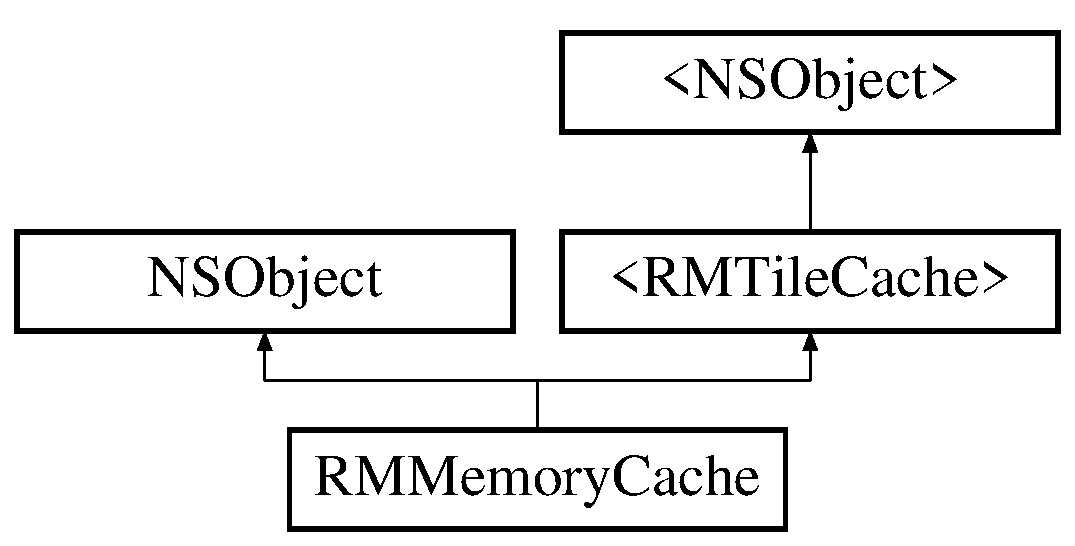
\includegraphics[height=3.000000cm]{interface_r_m_memory_cache}
\end{center}
\end{figure}
\subsection*{Instance Methods}
\begin{DoxyCompactItemize}
\item 
(void) -\/ \hyperlink{interface_r_m_memory_cache_a2f5b236d0de0767e8432014c46c9d7aa}{add\-Tile\-:\-With\-Image\-:}{\ttfamily  \mbox{[}implementation\mbox{]}}
\item 
(\hyperlink{interface_r_m_tile_image}{R\-M\-Tile\-Image} $\ast$) -\/ \hyperlink{interface_r_m_memory_cache_a701b5798480a1a5b7b17d16a0e919218}{cached\-Image\-:}{\ttfamily  \mbox{[}implementation\mbox{]}}
\begin{DoxyCompactList}\small\item\em Returns the cached image if it exists. nil otherwise. \end{DoxyCompactList}\item 
(void) -\/ \hyperlink{interface_r_m_memory_cache_a24a0d4acc108972b519a384e5ed17239}{dealloc}{\ttfamily  \mbox{[}implementation\mbox{]}}
\item 
(void) -\/ \hyperlink{interface_r_m_memory_cache_a39f0e5649c17432eb1369a7157ec0976}{did\-Receive\-Memory\-Warning}{\ttfamily  \mbox{[}implementation\mbox{]}}
\item 
(void) -\/ \hyperlink{interface_r_m_memory_cache_a40834ecc9d8c29ecdbb193d52e1cd7cf}{image\-Loading\-Cancelled\-:}{\ttfamily  \mbox{[}implementation\mbox{]}}
\item 
(id) -\/ \hyperlink{interface_r_m_memory_cache_ad00544180919205d1de0f053620b13de}{init}{\ttfamily  \mbox{[}implementation\mbox{]}}
\item 
(id) -\/ \hyperlink{interface_r_m_memory_cache_a4dfa721402ac7e524be00528ec0cee57}{init\-With\-Capacity\-:}
\item 
(void) -\/ \hyperlink{interface_r_m_memory_cache_a8398cac64d69583ba684081cbbdabf9c}{make\-Space\-In\-Cache}
\begin{DoxyCompactList}\small\item\em Remove the least-\/recently used image from cache, if cache is at or over capacity. Removes only 1 image. \end{DoxyCompactList}\item 
(void) -\/ \hyperlink{interface_r_m_memory_cache_ab46c85497105416077a467aaa917afce}{remove\-All\-Cached\-Images}{\ttfamily  \mbox{[}implementation\mbox{]}}
\begin{DoxyCompactList}\small\item\em removes all tile images from the memory and disk subcaches \end{DoxyCompactList}\item 
(void) -\/ \hyperlink{interface_r_m_memory_cache_ac859b7f94dd2c8af9f1ef1c77271a171}{remove\-Tile\-:}{\ttfamily  \mbox{[}implementation\mbox{]}}
\end{DoxyCompactItemize}
\subsection*{Protected 属性}
\begin{DoxyCompactItemize}
\item 
N\-S\-Mutable\-Dictionary $\ast$ \hyperlink{interface_r_m_memory_cache_a8e9bad5e8d5ae61cc4fe9d9a64f9d8da}{cache}
\item 
int \hyperlink{interface_r_m_memory_cache_a54f6971b0c858f13423b26ba6bf5633e}{capacity}
\end{DoxyCompactItemize}


\subsection{Method Documentation}
\hypertarget{interface_r_m_memory_cache_a2f5b236d0de0767e8432014c46c9d7aa}{\index{R\-M\-Memory\-Cache@{R\-M\-Memory\-Cache}!add\-Tile\-:\-With\-Image\-:@{add\-Tile\-:\-With\-Image\-:}}
\index{add\-Tile\-:\-With\-Image\-:@{add\-Tile\-:\-With\-Image\-:}!RMMemoryCache@{R\-M\-Memory\-Cache}}
\subsubsection[{add\-Tile\-:\-With\-Image\-:}]{\setlength{\rightskip}{0pt plus 5cm}-\/ (void) add\-Tile\-: 
\begin{DoxyParamCaption}
\item[{({\bf R\-M\-Tile})}]{tile}
\item[{WithImage:({\bf R\-M\-Tile\-Image}$\ast$)}]{image}
\end{DoxyParamCaption}
\hspace{0.3cm}{\ttfamily [implementation]}}}\label{interface_r_m_memory_cache_a2f5b236d0de0767e8432014c46c9d7aa}


重载 \hyperlink{protocol_r_m_tile_cache-p_a6a8e29b5f172b347d0ca556a643ee87c}{$<$\-R\-M\-Tile\-Cache$>$} .

\hypertarget{interface_r_m_memory_cache_a701b5798480a1a5b7b17d16a0e919218}{\index{R\-M\-Memory\-Cache@{R\-M\-Memory\-Cache}!cached\-Image\-:@{cached\-Image\-:}}
\index{cached\-Image\-:@{cached\-Image\-:}!RMMemoryCache@{R\-M\-Memory\-Cache}}
\subsubsection[{cached\-Image\-:}]{\setlength{\rightskip}{0pt plus 5cm}-\/ ({\bf R\-M\-Tile\-Image} $\ast$) cached\-Image\-: 
\begin{DoxyParamCaption}
\item[{({\bf R\-M\-Tile})}]{tile}
\end{DoxyParamCaption}
\hspace{0.3cm}{\ttfamily [implementation]}}}\label{interface_r_m_memory_cache_a701b5798480a1a5b7b17d16a0e919218}


Returns the cached image if it exists. nil otherwise. 



重载 \hyperlink{protocol_r_m_tile_cache-p_a4710bfa32e9aa99e8c8f6a335fcadbc2}{$<$\-R\-M\-Tile\-Cache$>$} .

\hypertarget{interface_r_m_memory_cache_a24a0d4acc108972b519a384e5ed17239}{\index{R\-M\-Memory\-Cache@{R\-M\-Memory\-Cache}!dealloc@{dealloc}}
\index{dealloc@{dealloc}!RMMemoryCache@{R\-M\-Memory\-Cache}}
\subsubsection[{dealloc}]{\setlength{\rightskip}{0pt plus 5cm}-\/ (void) dealloc 
\begin{DoxyParamCaption}
{}
\end{DoxyParamCaption}
\hspace{0.3cm}{\ttfamily [implementation]}}}\label{interface_r_m_memory_cache_a24a0d4acc108972b519a384e5ed17239}
\hypertarget{interface_r_m_memory_cache_a39f0e5649c17432eb1369a7157ec0976}{\index{R\-M\-Memory\-Cache@{R\-M\-Memory\-Cache}!did\-Receive\-Memory\-Warning@{did\-Receive\-Memory\-Warning}}
\index{did\-Receive\-Memory\-Warning@{did\-Receive\-Memory\-Warning}!RMMemoryCache@{R\-M\-Memory\-Cache}}
\subsubsection[{did\-Receive\-Memory\-Warning}]{\setlength{\rightskip}{0pt plus 5cm}-\/ (void) did\-Receive\-Memory\-Warning 
\begin{DoxyParamCaption}
{}
\end{DoxyParamCaption}
\hspace{0.3cm}{\ttfamily [implementation]}}}\label{interface_r_m_memory_cache_a39f0e5649c17432eb1369a7157ec0976}


重载 \hyperlink{protocol_r_m_tile_cache-p_abd8c91f7aeefeeb8744537ed2f304449}{$<$\-R\-M\-Tile\-Cache$>$} .

\hypertarget{interface_r_m_memory_cache_a40834ecc9d8c29ecdbb193d52e1cd7cf}{\index{R\-M\-Memory\-Cache@{R\-M\-Memory\-Cache}!image\-Loading\-Cancelled\-:@{image\-Loading\-Cancelled\-:}}
\index{image\-Loading\-Cancelled\-:@{image\-Loading\-Cancelled\-:}!RMMemoryCache@{R\-M\-Memory\-Cache}}
\subsubsection[{image\-Loading\-Cancelled\-:}]{\setlength{\rightskip}{0pt plus 5cm}-\/ (void) image\-Loading\-Cancelled\-: 
\begin{DoxyParamCaption}
\item[{(N\-S\-Notification$\ast$)}]{notification}
\end{DoxyParamCaption}
\hspace{0.3cm}{\ttfamily [implementation]}}}\label{interface_r_m_memory_cache_a40834ecc9d8c29ecdbb193d52e1cd7cf}
\hypertarget{interface_r_m_memory_cache_ad00544180919205d1de0f053620b13de}{\index{R\-M\-Memory\-Cache@{R\-M\-Memory\-Cache}!init@{init}}
\index{init@{init}!RMMemoryCache@{R\-M\-Memory\-Cache}}
\subsubsection[{init}]{\setlength{\rightskip}{0pt plus 5cm}-\/ (id) init 
\begin{DoxyParamCaption}
{}
\end{DoxyParamCaption}
\hspace{0.3cm}{\ttfamily [implementation]}}}\label{interface_r_m_memory_cache_ad00544180919205d1de0f053620b13de}
\begin{DoxyRefDesc}{Bug}
\item[\hyperlink{bug__bug000031}{Bug}]magic number \end{DoxyRefDesc}


参考自 init\-With\-Capacity\-:.

\hypertarget{interface_r_m_memory_cache_a4dfa721402ac7e524be00528ec0cee57}{\index{R\-M\-Memory\-Cache@{R\-M\-Memory\-Cache}!init\-With\-Capacity\-:@{init\-With\-Capacity\-:}}
\index{init\-With\-Capacity\-:@{init\-With\-Capacity\-:}!RMMemoryCache@{R\-M\-Memory\-Cache}}
\subsubsection[{init\-With\-Capacity\-:}]{\setlength{\rightskip}{0pt plus 5cm}-\/ (id) init\-With\-Capacity\-: 
\begin{DoxyParamCaption}
\item[{(N\-S\-U\-Integer)}]{\-\_\-capacity}
\end{DoxyParamCaption}
}}\label{interface_r_m_memory_cache_a4dfa721402ac7e524be00528ec0cee57}


参考自 init.

\hypertarget{interface_r_m_memory_cache_a8398cac64d69583ba684081cbbdabf9c}{\index{R\-M\-Memory\-Cache@{R\-M\-Memory\-Cache}!make\-Space\-In\-Cache@{make\-Space\-In\-Cache}}
\index{make\-Space\-In\-Cache@{make\-Space\-In\-Cache}!RMMemoryCache@{R\-M\-Memory\-Cache}}
\subsubsection[{make\-Space\-In\-Cache}]{\setlength{\rightskip}{0pt plus 5cm}-\/ (void) make\-Space\-In\-Cache 
\begin{DoxyParamCaption}
{}
\end{DoxyParamCaption}
}}\label{interface_r_m_memory_cache_a8398cac64d69583ba684081cbbdabf9c}


Remove the least-\/recently used image from cache, if cache is at or over capacity. Removes only 1 image. 



参考自 add\-Tile\-:\-With\-Image\-:.

\hypertarget{interface_r_m_memory_cache_ab46c85497105416077a467aaa917afce}{\index{R\-M\-Memory\-Cache@{R\-M\-Memory\-Cache}!remove\-All\-Cached\-Images@{remove\-All\-Cached\-Images}}
\index{remove\-All\-Cached\-Images@{remove\-All\-Cached\-Images}!RMMemoryCache@{R\-M\-Memory\-Cache}}
\subsubsection[{remove\-All\-Cached\-Images}]{\setlength{\rightskip}{0pt plus 5cm}-\/ (void) remove\-All\-Cached\-Images 
\begin{DoxyParamCaption}
{}
\end{DoxyParamCaption}
\hspace{0.3cm}{\ttfamily [implementation]}}}\label{interface_r_m_memory_cache_ab46c85497105416077a467aaa917afce}


removes all tile images from the memory and disk subcaches 



重载 \hyperlink{protocol_r_m_tile_cache-p_a57f54af62bb9c0e473ba2cd395864c4a}{$<$\-R\-M\-Tile\-Cache$>$} .

\hypertarget{interface_r_m_memory_cache_ac859b7f94dd2c8af9f1ef1c77271a171}{\index{R\-M\-Memory\-Cache@{R\-M\-Memory\-Cache}!remove\-Tile\-:@{remove\-Tile\-:}}
\index{remove\-Tile\-:@{remove\-Tile\-:}!RMMemoryCache@{R\-M\-Memory\-Cache}}
\subsubsection[{remove\-Tile\-:}]{\setlength{\rightskip}{0pt plus 5cm}-\/ (void) remove\-Tile\-: 
\begin{DoxyParamCaption}
\item[{({\bf R\-M\-Tile})}]{tile}
\end{DoxyParamCaption}
\hspace{0.3cm}{\ttfamily [implementation]}}}\label{interface_r_m_memory_cache_ac859b7f94dd2c8af9f1ef1c77271a171}


参考自 image\-Loading\-Cancelled\-: , 以及 make\-Space\-In\-Cache.



\subsection{类成员变量说明}
\hypertarget{interface_r_m_memory_cache_a8e9bad5e8d5ae61cc4fe9d9a64f9d8da}{\index{R\-M\-Memory\-Cache@{R\-M\-Memory\-Cache}!cache@{cache}}
\index{cache@{cache}!RMMemoryCache@{R\-M\-Memory\-Cache}}
\subsubsection[{cache}]{\setlength{\rightskip}{0pt plus 5cm}-\/ (N\-S\-Mutable\-Dictionary$\ast$) cache\hspace{0.3cm}{\ttfamily [protected]}}}\label{interface_r_m_memory_cache_a8e9bad5e8d5ae61cc4fe9d9a64f9d8da}


参考自 add\-Tile\-:\-With\-Image\-:, cached\-Image\-:, dealloc, did\-Receive\-Memory\-Warning, init\-With\-Capacity\-:, make\-Space\-In\-Cache, remove\-All\-Cached\-Images , 以及 remove\-Tile\-:.

\hypertarget{interface_r_m_memory_cache_a54f6971b0c858f13423b26ba6bf5633e}{\index{R\-M\-Memory\-Cache@{R\-M\-Memory\-Cache}!capacity@{capacity}}
\index{capacity@{capacity}!RMMemoryCache@{R\-M\-Memory\-Cache}}
\subsubsection[{capacity}]{\setlength{\rightskip}{0pt plus 5cm}-\/ (int) capacity\hspace{0.3cm}{\ttfamily [protected]}}}\label{interface_r_m_memory_cache_a54f6971b0c858f13423b26ba6bf5633e}


参考自 init\-With\-Capacity\-: , 以及 make\-Space\-In\-Cache.



该类的文档由以下文件生成\-:\begin{DoxyCompactItemize}
\item 
Map/\hyperlink{_r_m_memory_cache_8h}{R\-M\-Memory\-Cache.\-h}\item 
Map/\hyperlink{_r_m_memory_cache_8m}{R\-M\-Memory\-Cache.\-m}\end{DoxyCompactItemize}

\hypertarget{interface_r_m_mercator_to_screen_projection}{\section{R\-M\-Mercator\-To\-Screen\-Projection类 参考}
\label{interface_r_m_mercator_to_screen_projection}\index{R\-M\-Mercator\-To\-Screen\-Projection@{R\-M\-Mercator\-To\-Screen\-Projection}}
}


This is a stateful projection. As the screen moves around, so too do projections change.  




{\ttfamily \#import $<$R\-M\-Mercator\-To\-Screen\-Projection.\-h$>$}

类 R\-M\-Mercator\-To\-Screen\-Projection 继承关系图\-:\begin{figure}[H]
\begin{center}
\leavevmode
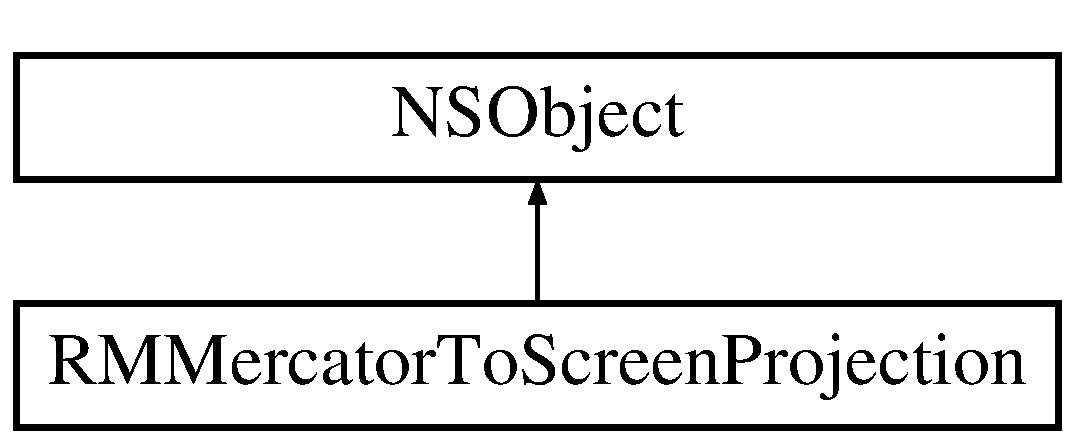
\includegraphics[height=2.000000cm]{interface_r_m_mercator_to_screen_projection}
\end{center}
\end{figure}
\subsection*{Instance Methods}
\begin{DoxyCompactItemize}
\item 
(void) -\/ \hyperlink{interface_r_m_mercator_to_screen_projection_a10a96f474830fac6431f2b5521187397}{dealloc}{\ttfamily  \mbox{[}implementation\mbox{]}}
\item 
(void) -\/ \hyperlink{interface_r_m_mercator_to_screen_projection_a6c4a7f6af88955ab4123a4f5bc14f935}{deep\-Copy\-:}
\item 
(id) -\/ \hyperlink{interface_r_m_mercator_to_screen_projection_a6e3bab2a43cbc3c17295f63d34f7df10}{init\-From\-Projection\-:\-To\-Screen\-Bounds\-:}
\item 
(\hyperlink{struct_r_m_projected_point}{R\-M\-Projected\-Point}) -\/ \hyperlink{interface_r_m_mercator_to_screen_projection_af1262b51fc47cc2f4a4424e6e5fcfc79}{move\-Point\-:by\-:}
\begin{DoxyCompactList}\small\item\em Deltas in screen coordinates. \end{DoxyCompactList}\item 
(\hyperlink{struct_r_m_projected_rect}{R\-M\-Projected\-Rect}) -\/ \hyperlink{interface_r_m_mercator_to_screen_projection_a43f1802cb7c5c9d3bb518ee32fc5d8b5}{move\-Rect\-:by\-:}
\begin{DoxyCompactList}\small\item\em Deltas in screen coordinates. \end{DoxyCompactList}\item 
(void) -\/ \hyperlink{interface_r_m_mercator_to_screen_projection_a47cfe6fc7b295e1eacad2fea309b1840}{move\-Screen\-By\-:}
\begin{DoxyCompactList}\small\item\em Move the screen. \end{DoxyCompactList}\item 
(\hyperlink{struct_r_m_projected_rect}{R\-M\-Projected\-Rect}) -\/ \hyperlink{interface_r_m_mercator_to_screen_projection_adc63aa7ec95b73a89d4839d6851a0030}{projected\-Bounds}
\item 
(\hyperlink{struct_r_m_projected_point}{R\-M\-Projected\-Point}) -\/ \hyperlink{interface_r_m_mercator_to_screen_projection_a0be470e222397c01d1fbc343c958c4ed}{projected\-Center}
\item 
(\hyperlink{struct_r_m_projected_point}{R\-M\-Projected\-Point}) -\/ \hyperlink{interface_r_m_mercator_to_screen_projection_a079490067b3f7dd5326389720f383049}{project\-Screen\-Point\-To\-X\-Y\-:}
\item 
(\hyperlink{struct_r_m_projected_point}{R\-M\-Projected\-Point}) -\/ \hyperlink{interface_r_m_mercator_to_screen_projection_ae4aca2604d100a8a16e04f70c7d7740e}{project\-Screen\-Point\-To\-X\-Y\-:with\-Meters\-Per\-Pixel\-:}
\item 
(\hyperlink{struct_r_m_projected_rect}{R\-M\-Projected\-Rect}) -\/ \hyperlink{interface_r_m_mercator_to_screen_projection_a52b275b603a3ce0ecae8d8126880252c}{project\-Screen\-Rect\-To\-X\-Y\-:}
\item 
(\hyperlink{struct_r_m_projected_size}{R\-M\-Projected\-Size}) -\/ \hyperlink{interface_r_m_mercator_to_screen_projection_a36883ed7966071c5f51a836c77a2f2da}{project\-Screen\-Size\-To\-X\-Y\-:}
\item 
(C\-G\-Point) -\/ \hyperlink{interface_r_m_mercator_to_screen_projection_a276efafa172d9221c5133d2308890c8f}{project\-X\-Y\-Point\-:}
\begin{DoxyCompactList}\small\item\em Project -\/$>$ screen coordinates. \end{DoxyCompactList}\item 
(C\-G\-Point) -\/ \hyperlink{interface_r_m_mercator_to_screen_projection_afbe204c10488ebc50a818d88d0017b16}{project\-X\-Y\-Point\-:with\-Meters\-Per\-Pixel\-:}
\begin{DoxyCompactList}\small\item\em Project -\/$>$ screen coordinates. \end{DoxyCompactList}\item 
(C\-G\-Rect) -\/ \hyperlink{interface_r_m_mercator_to_screen_projection_a1d5076b8f0b97d2b93a7d801c61f8ba4}{project\-X\-Y\-Rect\-:}
\begin{DoxyCompactList}\small\item\em Project -\/$>$ screen coordinates. \end{DoxyCompactList}\item 
(C\-G\-Rect) -\/ \hyperlink{interface_r_m_mercator_to_screen_projection_aebb472dbe94a24c62a612fa849732d39}{screen\-Bounds}
\item 
(void) -\/ \hyperlink{interface_r_m_mercator_to_screen_projection_ac8c6b2da4ecc190c768b4e30469b410b}{set\-Meters\-Per\-Pixel\-:}{\ttfamily  \mbox{[}implementation\mbox{]}}
\item 
(void) -\/ \hyperlink{interface_r_m_mercator_to_screen_projection_a0e7573981b462d019a879178840233f4}{set\-Projected\-Bounds\-:}
\item 
(void) -\/ \hyperlink{interface_r_m_mercator_to_screen_projection_a814a8a8ddbafeda6e68b8e02d2efcfb4}{set\-Projected\-Center\-:}
\item 
(void) -\/ \hyperlink{interface_r_m_mercator_to_screen_projection_ab2bd98049aaf4340cb2291b13588f77d}{set\-Screen\-Bounds\-:}
\item 
(void) -\/ \hyperlink{interface_r_m_mercator_to_screen_projection_a0882ed84fe7346f3a9b8f4e63e2dfa0a}{zoom\-By\-:}{\ttfamily  \mbox{[}implementation\mbox{]}}
\item 
(\hyperlink{struct_r_m_projected_point}{R\-M\-Projected\-Point}) -\/ \hyperlink{interface_r_m_mercator_to_screen_projection_a5cb02ad7176d0523eb57471fc99e3c7c}{zoom\-Point\-:by\-Factor\-:near\-:}
\begin{DoxyCompactList}\small\item\em pivot given in screen coordinates. \end{DoxyCompactList}\item 
(\hyperlink{struct_r_m_projected_rect}{R\-M\-Projected\-Rect}) -\/ \hyperlink{interface_r_m_mercator_to_screen_projection_a99a67d660114f633f116ebf688642cdc}{zoom\-Rect\-:by\-Factor\-:near\-:}
\begin{DoxyCompactList}\small\item\em pivot given in screen coordinates. \end{DoxyCompactList}\item 
(void) -\/ \hyperlink{interface_r_m_mercator_to_screen_projection_ad47c361352cdff2e4689721db9fb6c52}{zoom\-Screen\-By\-Factor\-:near\-:}
\end{DoxyCompactItemize}
\subsection*{Protected 属性}
\begin{DoxyCompactItemize}
\item 
C\-G\-Rect \hyperlink{interface_r_m_mercator_to_screen_projection_ac28d9acefc1c419405f7331d9038675a}{screen\-Bounds}
\begin{DoxyCompactList}\small\item\em Bounds of the screen in pixels. \end{DoxyCompactList}\end{DoxyCompactItemize}
\subsection*{属性}
\begin{DoxyCompactItemize}
\item 
float \hyperlink{interface_r_m_mercator_to_screen_projection_a6e73179ce2febd38c2f8baefedfefc47}{meters\-Per\-Pixel}
\begin{DoxyCompactList}\small\item\em meters per pixel \end{DoxyCompactList}\item 
\hyperlink{struct_r_m_projected_point}{R\-M\-Projected\-Point} \hyperlink{interface_r_m_mercator_to_screen_projection_abc3cfe961a255f28bb2ea051ae2cbaf5}{origin}
\begin{DoxyCompactList}\small\item\em What the screen is currently looking at. \end{DoxyCompactList}\item 
\hyperlink{interface_r_m_projection}{R\-M\-Projection} $\ast$ \hyperlink{interface_r_m_mercator_to_screen_projection_a410f2049effa29cfceb4fa87f77b3f22}{projection}
\begin{DoxyCompactList}\small\item\em The mercator -\/or-\/whatever-\/ projection that the map is in. \end{DoxyCompactList}\end{DoxyCompactItemize}


\subsection{详细描述}
This is a stateful projection. As the screen moves around, so too do projections change. 

\subsection{Method Documentation}
\hypertarget{interface_r_m_mercator_to_screen_projection_a10a96f474830fac6431f2b5521187397}{\index{R\-M\-Mercator\-To\-Screen\-Projection@{R\-M\-Mercator\-To\-Screen\-Projection}!dealloc@{dealloc}}
\index{dealloc@{dealloc}!RMMercatorToScreenProjection@{R\-M\-Mercator\-To\-Screen\-Projection}}
\subsubsection[{dealloc}]{\setlength{\rightskip}{0pt plus 5cm}-\/ (void) dealloc 
\begin{DoxyParamCaption}
{}
\end{DoxyParamCaption}
\hspace{0.3cm}{\ttfamily [implementation]}}}\label{interface_r_m_mercator_to_screen_projection_a10a96f474830fac6431f2b5521187397}
\hypertarget{interface_r_m_mercator_to_screen_projection_a6c4a7f6af88955ab4123a4f5bc14f935}{\index{R\-M\-Mercator\-To\-Screen\-Projection@{R\-M\-Mercator\-To\-Screen\-Projection}!deep\-Copy\-:@{deep\-Copy\-:}}
\index{deep\-Copy\-:@{deep\-Copy\-:}!RMMercatorToScreenProjection@{R\-M\-Mercator\-To\-Screen\-Projection}}
\subsubsection[{deep\-Copy\-:}]{\setlength{\rightskip}{0pt plus 5cm}-\/ (void) deep\-Copy\-: 
\begin{DoxyParamCaption}
\item[{({\bf R\-M\-Mercator\-To\-Screen\-Projection} $\ast$)}]{copy}
\end{DoxyParamCaption}
}}\label{interface_r_m_mercator_to_screen_projection_a6c4a7f6af88955ab4123a4f5bc14f935}
\hypertarget{interface_r_m_mercator_to_screen_projection_a6e3bab2a43cbc3c17295f63d34f7df10}{\index{R\-M\-Mercator\-To\-Screen\-Projection@{R\-M\-Mercator\-To\-Screen\-Projection}!init\-From\-Projection\-:\-To\-Screen\-Bounds\-:@{init\-From\-Projection\-:\-To\-Screen\-Bounds\-:}}
\index{init\-From\-Projection\-:\-To\-Screen\-Bounds\-:@{init\-From\-Projection\-:\-To\-Screen\-Bounds\-:}!RMMercatorToScreenProjection@{R\-M\-Mercator\-To\-Screen\-Projection}}
\subsubsection[{init\-From\-Projection\-:\-To\-Screen\-Bounds\-:}]{\setlength{\rightskip}{0pt plus 5cm}-\/ (id) init\-From\-Projection\-: 
\begin{DoxyParamCaption}
\item[{({\bf R\-M\-Projection}$\ast$)}]{projection}
\item[{ToScreenBounds:(C\-G\-Rect)}]{a\-Screen\-Bounds}
\end{DoxyParamCaption}
}}\label{interface_r_m_mercator_to_screen_projection_a6e3bab2a43cbc3c17295f63d34f7df10}
\hypertarget{interface_r_m_mercator_to_screen_projection_af1262b51fc47cc2f4a4424e6e5fcfc79}{\index{R\-M\-Mercator\-To\-Screen\-Projection@{R\-M\-Mercator\-To\-Screen\-Projection}!move\-Point\-:by\-:@{move\-Point\-:by\-:}}
\index{move\-Point\-:by\-:@{move\-Point\-:by\-:}!RMMercatorToScreenProjection@{R\-M\-Mercator\-To\-Screen\-Projection}}
\subsubsection[{move\-Point\-:by\-:}]{\setlength{\rightskip}{0pt plus 5cm}-\/ ({\bf R\-M\-Projected\-Point}) move\-Point\-: 
\begin{DoxyParamCaption}
\item[{({\bf R\-M\-Projected\-Point})}]{a\-Point}
\item[{by:(C\-G\-Size)}]{delta}
\end{DoxyParamCaption}
}}\label{interface_r_m_mercator_to_screen_projection_af1262b51fc47cc2f4a4424e6e5fcfc79}


Deltas in screen coordinates. 



参考自 move\-Rect\-:by\-: , 以及 move\-Screen\-By\-:.

\hypertarget{interface_r_m_mercator_to_screen_projection_a43f1802cb7c5c9d3bb518ee32fc5d8b5}{\index{R\-M\-Mercator\-To\-Screen\-Projection@{R\-M\-Mercator\-To\-Screen\-Projection}!move\-Rect\-:by\-:@{move\-Rect\-:by\-:}}
\index{move\-Rect\-:by\-:@{move\-Rect\-:by\-:}!RMMercatorToScreenProjection@{R\-M\-Mercator\-To\-Screen\-Projection}}
\subsubsection[{move\-Rect\-:by\-:}]{\setlength{\rightskip}{0pt plus 5cm}-\/ ({\bf R\-M\-Projected\-Rect}) move\-Rect\-: 
\begin{DoxyParamCaption}
\item[{({\bf R\-M\-Projected\-Rect})}]{a\-Rect}
\item[{by:(C\-G\-Size)}]{delta}
\end{DoxyParamCaption}
}}\label{interface_r_m_mercator_to_screen_projection_a43f1802cb7c5c9d3bb518ee32fc5d8b5}


Deltas in screen coordinates. 

\hypertarget{interface_r_m_mercator_to_screen_projection_a47cfe6fc7b295e1eacad2fea309b1840}{\index{R\-M\-Mercator\-To\-Screen\-Projection@{R\-M\-Mercator\-To\-Screen\-Projection}!move\-Screen\-By\-:@{move\-Screen\-By\-:}}
\index{move\-Screen\-By\-:@{move\-Screen\-By\-:}!RMMercatorToScreenProjection@{R\-M\-Mercator\-To\-Screen\-Projection}}
\subsubsection[{move\-Screen\-By\-:}]{\setlength{\rightskip}{0pt plus 5cm}-\/ (void) move\-Screen\-By\-: 
\begin{DoxyParamCaption}
\item[{(C\-G\-Size)}]{delta}
\end{DoxyParamCaption}
}}\label{interface_r_m_mercator_to_screen_projection_a47cfe6fc7b295e1eacad2fea309b1840}


Move the screen. 



参考自 R\-M\-Map\-Contents\-::move\-By\-:.

\hypertarget{interface_r_m_mercator_to_screen_projection_adc63aa7ec95b73a89d4839d6851a0030}{\index{R\-M\-Mercator\-To\-Screen\-Projection@{R\-M\-Mercator\-To\-Screen\-Projection}!projected\-Bounds@{projected\-Bounds}}
\index{projected\-Bounds@{projected\-Bounds}!RMMercatorToScreenProjection@{R\-M\-Mercator\-To\-Screen\-Projection}}
\subsubsection[{projected\-Bounds}]{\setlength{\rightskip}{0pt plus 5cm}-\/ ({\bf R\-M\-Projected\-Rect}) projected\-Bounds 
\begin{DoxyParamCaption}
{}
\end{DoxyParamCaption}
}}\label{interface_r_m_mercator_to_screen_projection_adc63aa7ec95b73a89d4839d6851a0030}


参考自 R\-M\-Map\-View\-::move\-By\-:, R\-M\-S\-M\-Tile\-Projection\-::project\-: , 以及 R\-M\-Fractal\-Tile\-Projection\-::project\-:.

\hypertarget{interface_r_m_mercator_to_screen_projection_a0be470e222397c01d1fbc343c958c4ed}{\index{R\-M\-Mercator\-To\-Screen\-Projection@{R\-M\-Mercator\-To\-Screen\-Projection}!projected\-Center@{projected\-Center}}
\index{projected\-Center@{projected\-Center}!RMMercatorToScreenProjection@{R\-M\-Mercator\-To\-Screen\-Projection}}
\subsubsection[{projected\-Center}]{\setlength{\rightskip}{0pt plus 5cm}-\/ ({\bf R\-M\-Projected\-Point}) projected\-Center 
\begin{DoxyParamCaption}
{}
\end{DoxyParamCaption}
}}\label{interface_r_m_mercator_to_screen_projection_a0be470e222397c01d1fbc343c958c4ed}


参考自 set\-Meters\-Per\-Pixel\-:.

\hypertarget{interface_r_m_mercator_to_screen_projection_a079490067b3f7dd5326389720f383049}{\index{R\-M\-Mercator\-To\-Screen\-Projection@{R\-M\-Mercator\-To\-Screen\-Projection}!project\-Screen\-Point\-To\-X\-Y\-:@{project\-Screen\-Point\-To\-X\-Y\-:}}
\index{project\-Screen\-Point\-To\-X\-Y\-:@{project\-Screen\-Point\-To\-X\-Y\-:}!RMMercatorToScreenProjection@{R\-M\-Mercator\-To\-Screen\-Projection}}
\subsubsection[{project\-Screen\-Point\-To\-X\-Y\-:}]{\setlength{\rightskip}{0pt plus 5cm}-\/ ({\bf R\-M\-Projected\-Point}) project\-Screen\-Point\-To\-X\-Y\-: 
\begin{DoxyParamCaption}
\item[{(C\-G\-Point)}]{a\-Point}
\end{DoxyParamCaption}
}}\label{interface_r_m_mercator_to_screen_projection_a079490067b3f7dd5326389720f383049}


参考自 R\-M\-Path\-::add\-Line\-To\-Screen\-Point\-:, R\-M\-Marker\-Manager\-::move\-Marker\-:\-At\-X\-Y\-:, R\-M\-Path\-::move\-To\-Screen\-Point\-:, R\-M\-Map\-Contents\-::pixel\-To\-Lat\-Long\-:, project\-Screen\-Rect\-To\-X\-Y\-:, zoom\-Point\-:by\-Factor\-:near\-: , 以及 zoom\-Rect\-:by\-Factor\-:near\-:.

\hypertarget{interface_r_m_mercator_to_screen_projection_ae4aca2604d100a8a16e04f70c7d7740e}{\index{R\-M\-Mercator\-To\-Screen\-Projection@{R\-M\-Mercator\-To\-Screen\-Projection}!project\-Screen\-Point\-To\-X\-Y\-:with\-Meters\-Per\-Pixel\-:@{project\-Screen\-Point\-To\-X\-Y\-:with\-Meters\-Per\-Pixel\-:}}
\index{project\-Screen\-Point\-To\-X\-Y\-:with\-Meters\-Per\-Pixel\-:@{project\-Screen\-Point\-To\-X\-Y\-:with\-Meters\-Per\-Pixel\-:}!RMMercatorToScreenProjection@{R\-M\-Mercator\-To\-Screen\-Projection}}
\subsubsection[{project\-Screen\-Point\-To\-X\-Y\-:with\-Meters\-Per\-Pixel\-:}]{\setlength{\rightskip}{0pt plus 5cm}-\/ ({\bf R\-M\-Projected\-Point}) {\bf project\-Screen\-Point\-To\-X\-Y\-:} 
\begin{DoxyParamCaption}
\item[{(C\-G\-Point)}]{a\-Pixel\-Point}
\item[{withMetersPerPixel:(float)}]{a\-Scale}
\end{DoxyParamCaption}
}}\label{interface_r_m_mercator_to_screen_projection_ae4aca2604d100a8a16e04f70c7d7740e}


参考自 R\-M\-Map\-Contents\-::pixel\-To\-Lat\-Long\-:with\-Meters\-Per\-Pixel\-: , 以及 project\-Screen\-Point\-To\-X\-Y\-:.

\hypertarget{interface_r_m_mercator_to_screen_projection_a52b275b603a3ce0ecae8d8126880252c}{\index{R\-M\-Mercator\-To\-Screen\-Projection@{R\-M\-Mercator\-To\-Screen\-Projection}!project\-Screen\-Rect\-To\-X\-Y\-:@{project\-Screen\-Rect\-To\-X\-Y\-:}}
\index{project\-Screen\-Rect\-To\-X\-Y\-:@{project\-Screen\-Rect\-To\-X\-Y\-:}!RMMercatorToScreenProjection@{R\-M\-Mercator\-To\-Screen\-Projection}}
\subsubsection[{project\-Screen\-Rect\-To\-X\-Y\-:}]{\setlength{\rightskip}{0pt plus 5cm}-\/ ({\bf R\-M\-Projected\-Rect}) project\-Screen\-Rect\-To\-X\-Y\-: 
\begin{DoxyParamCaption}
\item[{(C\-G\-Rect)}]{a\-Rect}
\end{DoxyParamCaption}
}}\label{interface_r_m_mercator_to_screen_projection_a52b275b603a3ce0ecae8d8126880252c}
\hypertarget{interface_r_m_mercator_to_screen_projection_a36883ed7966071c5f51a836c77a2f2da}{\index{R\-M\-Mercator\-To\-Screen\-Projection@{R\-M\-Mercator\-To\-Screen\-Projection}!project\-Screen\-Size\-To\-X\-Y\-:@{project\-Screen\-Size\-To\-X\-Y\-:}}
\index{project\-Screen\-Size\-To\-X\-Y\-:@{project\-Screen\-Size\-To\-X\-Y\-:}!RMMercatorToScreenProjection@{R\-M\-Mercator\-To\-Screen\-Projection}}
\subsubsection[{project\-Screen\-Size\-To\-X\-Y\-:}]{\setlength{\rightskip}{0pt plus 5cm}-\/ ({\bf R\-M\-Projected\-Size}) project\-Screen\-Size\-To\-X\-Y\-: 
\begin{DoxyParamCaption}
\item[{(C\-G\-Size)}]{a\-Size}
\end{DoxyParamCaption}
}}\label{interface_r_m_mercator_to_screen_projection_a36883ed7966071c5f51a836c77a2f2da}


参考自 R\-M\-Map\-View\-::move\-By\-: , 以及 move\-Point\-:by\-:.

\hypertarget{interface_r_m_mercator_to_screen_projection_a276efafa172d9221c5133d2308890c8f}{\index{R\-M\-Mercator\-To\-Screen\-Projection@{R\-M\-Mercator\-To\-Screen\-Projection}!project\-X\-Y\-Point\-:@{project\-X\-Y\-Point\-:}}
\index{project\-X\-Y\-Point\-:@{project\-X\-Y\-Point\-:}!RMMercatorToScreenProjection@{R\-M\-Mercator\-To\-Screen\-Projection}}
\subsubsection[{project\-X\-Y\-Point\-:}]{\setlength{\rightskip}{0pt plus 5cm}-\/ (C\-G\-Point) project\-X\-Y\-Point\-: 
\begin{DoxyParamCaption}
\item[{({\bf R\-M\-Projected\-Point})}]{a\-Point}
\end{DoxyParamCaption}
}}\label{interface_r_m_mercator_to_screen_projection_a276efafa172d9221c5133d2308890c8f}


Project -\/$>$ screen coordinates. 



参考自 R\-M\-Marker\-Manager\-::add\-Marker\-:at\-Projected\-Point\-:, R\-M\-Path\-::add\-Point\-To\-X\-Y\-:with\-Drawing\-:, R\-M\-Layer\-Collection\-::correct\-Screen\-Position\-:, R\-M\-Circle\-::init\-With\-Contents\-:radius\-In\-Meters\-:lat\-Long\-:, R\-M\-Map\-Contents\-::lat\-Long\-To\-Pixel\-:, R\-M\-Marker\-Manager\-::move\-Marker\-:\-At\-Lat\-Lon\-:, R\-M\-Circle\-::move\-To\-Lat\-Long\-:, project\-X\-Y\-Rect\-:, R\-M\-Path\-::recalculate\-Geometry, R\-M\-Marker\-Manager\-::screen\-Coordinates\-For\-Marker\-: , 以及 R\-M\-Circle\-::set\-Projected\-Location\-:.

\hypertarget{interface_r_m_mercator_to_screen_projection_afbe204c10488ebc50a818d88d0017b16}{\index{R\-M\-Mercator\-To\-Screen\-Projection@{R\-M\-Mercator\-To\-Screen\-Projection}!project\-X\-Y\-Point\-:with\-Meters\-Per\-Pixel\-:@{project\-X\-Y\-Point\-:with\-Meters\-Per\-Pixel\-:}}
\index{project\-X\-Y\-Point\-:with\-Meters\-Per\-Pixel\-:@{project\-X\-Y\-Point\-:with\-Meters\-Per\-Pixel\-:}!RMMercatorToScreenProjection@{R\-M\-Mercator\-To\-Screen\-Projection}}
\subsubsection[{project\-X\-Y\-Point\-:with\-Meters\-Per\-Pixel\-:}]{\setlength{\rightskip}{0pt plus 5cm}-\/ (C\-G\-Point) {\bf project\-X\-Y\-Point\-:} 
\begin{DoxyParamCaption}
\item[{({\bf R\-M\-Projected\-Point})}]{a\-Point}
\item[{withMetersPerPixel:(float)}]{a\-Scale}
\end{DoxyParamCaption}
}}\label{interface_r_m_mercator_to_screen_projection_afbe204c10488ebc50a818d88d0017b16}


Project -\/$>$ screen coordinates. 



参考自 R\-M\-Map\-Contents\-::lat\-Long\-To\-Pixel\-:with\-Meters\-Per\-Pixel\-: , 以及 project\-X\-Y\-Point\-:.

\hypertarget{interface_r_m_mercator_to_screen_projection_a1d5076b8f0b97d2b93a7d801c61f8ba4}{\index{R\-M\-Mercator\-To\-Screen\-Projection@{R\-M\-Mercator\-To\-Screen\-Projection}!project\-X\-Y\-Rect\-:@{project\-X\-Y\-Rect\-:}}
\index{project\-X\-Y\-Rect\-:@{project\-X\-Y\-Rect\-:}!RMMercatorToScreenProjection@{R\-M\-Mercator\-To\-Screen\-Projection}}
\subsubsection[{project\-X\-Y\-Rect\-:}]{\setlength{\rightskip}{0pt plus 5cm}-\/ (C\-G\-Rect) project\-X\-Y\-Rect\-: 
\begin{DoxyParamCaption}
\item[{({\bf R\-M\-Projected\-Rect})}]{a\-Rect}
\end{DoxyParamCaption}
}}\label{interface_r_m_mercator_to_screen_projection_a1d5076b8f0b97d2b93a7d801c61f8ba4}


Project -\/$>$ screen coordinates. 

\hypertarget{interface_r_m_mercator_to_screen_projection_aebb472dbe94a24c62a612fa849732d39}{\index{R\-M\-Mercator\-To\-Screen\-Projection@{R\-M\-Mercator\-To\-Screen\-Projection}!screen\-Bounds@{screen\-Bounds}}
\index{screen\-Bounds@{screen\-Bounds}!RMMercatorToScreenProjection@{R\-M\-Mercator\-To\-Screen\-Projection}}
\subsubsection[{screen\-Bounds}]{\setlength{\rightskip}{0pt plus 5cm}-\/ (C\-G\-Rect) screen\-Bounds 
\begin{DoxyParamCaption}
{}
\end{DoxyParamCaption}
}}\label{interface_r_m_mercator_to_screen_projection_aebb472dbe94a24c62a612fa849732d39}


参考自 deep\-Copy\-:, init\-From\-Projection\-:\-To\-Screen\-Bounds\-:, projected\-Bounds, projected\-Center, project\-Screen\-Point\-To\-X\-Y\-:with\-Meters\-Per\-Pixel\-:, project\-X\-Y\-Point\-:with\-Meters\-Per\-Pixel\-:, set\-Projected\-Bounds\-:, set\-Projected\-Center\-:, set\-Screen\-Bounds\-: , 以及 zoom\-Screen\-By\-Factor\-:near\-:.

\hypertarget{interface_r_m_mercator_to_screen_projection_ac8c6b2da4ecc190c768b4e30469b410b}{\index{R\-M\-Mercator\-To\-Screen\-Projection@{R\-M\-Mercator\-To\-Screen\-Projection}!set\-Meters\-Per\-Pixel\-:@{set\-Meters\-Per\-Pixel\-:}}
\index{set\-Meters\-Per\-Pixel\-:@{set\-Meters\-Per\-Pixel\-:}!RMMercatorToScreenProjection@{R\-M\-Mercator\-To\-Screen\-Projection}}
\subsubsection[{set\-Meters\-Per\-Pixel\-:}]{\setlength{\rightskip}{0pt plus 5cm}-\/ (void) set\-Meters\-Per\-Pixel\-: 
\begin{DoxyParamCaption}
\item[{(float)}]{new\-M\-P\-P}
\end{DoxyParamCaption}
\hspace{0.3cm}{\ttfamily [implementation]}}}\label{interface_r_m_mercator_to_screen_projection_ac8c6b2da4ecc190c768b4e30469b410b}


参考自 R\-M\-Map\-Contents\-::set\-Meters\-Per\-Pixel\-:.

\hypertarget{interface_r_m_mercator_to_screen_projection_a0e7573981b462d019a879178840233f4}{\index{R\-M\-Mercator\-To\-Screen\-Projection@{R\-M\-Mercator\-To\-Screen\-Projection}!set\-Projected\-Bounds\-:@{set\-Projected\-Bounds\-:}}
\index{set\-Projected\-Bounds\-:@{set\-Projected\-Bounds\-:}!RMMercatorToScreenProjection@{R\-M\-Mercator\-To\-Screen\-Projection}}
\subsubsection[{set\-Projected\-Bounds\-:}]{\setlength{\rightskip}{0pt plus 5cm}-\/ (void) set\-Projected\-Bounds\-: 
\begin{DoxyParamCaption}
\item[{({\bf R\-M\-Projected\-Rect})}]{bounds}
\end{DoxyParamCaption}
}}\label{interface_r_m_mercator_to_screen_projection_a0e7573981b462d019a879178840233f4}


参考自 R\-M\-Map\-Contents\-::set\-Projected\-Bounds\-:.

\hypertarget{interface_r_m_mercator_to_screen_projection_a814a8a8ddbafeda6e68b8e02d2efcfb4}{\index{R\-M\-Mercator\-To\-Screen\-Projection@{R\-M\-Mercator\-To\-Screen\-Projection}!set\-Projected\-Center\-:@{set\-Projected\-Center\-:}}
\index{set\-Projected\-Center\-:@{set\-Projected\-Center\-:}!RMMercatorToScreenProjection@{R\-M\-Mercator\-To\-Screen\-Projection}}
\subsubsection[{set\-Projected\-Center\-:}]{\setlength{\rightskip}{0pt plus 5cm}-\/ (void) set\-Projected\-Center\-: 
\begin{DoxyParamCaption}
\item[{({\bf R\-M\-Projected\-Point})}]{a\-Point}
\end{DoxyParamCaption}
}}\label{interface_r_m_mercator_to_screen_projection_a814a8a8ddbafeda6e68b8e02d2efcfb4}


参考自 R\-M\-Map\-Contents\-::set\-Center\-Projected\-Point\-: , 以及 set\-Meters\-Per\-Pixel\-:.

\hypertarget{interface_r_m_mercator_to_screen_projection_ab2bd98049aaf4340cb2291b13588f77d}{\index{R\-M\-Mercator\-To\-Screen\-Projection@{R\-M\-Mercator\-To\-Screen\-Projection}!set\-Screen\-Bounds\-:@{set\-Screen\-Bounds\-:}}
\index{set\-Screen\-Bounds\-:@{set\-Screen\-Bounds\-:}!RMMercatorToScreenProjection@{R\-M\-Mercator\-To\-Screen\-Projection}}
\subsubsection[{set\-Screen\-Bounds\-:}]{\setlength{\rightskip}{0pt plus 5cm}-\/ (void) set\-Screen\-Bounds\-: 
\begin{DoxyParamCaption}
\item[{(C\-G\-Rect)}]{rect}
\end{DoxyParamCaption}
}}\label{interface_r_m_mercator_to_screen_projection_ab2bd98049aaf4340cb2291b13588f77d}


参考自 R\-M\-Map\-Contents\-::set\-Frame\-:.

\hypertarget{interface_r_m_mercator_to_screen_projection_a0882ed84fe7346f3a9b8f4e63e2dfa0a}{\index{R\-M\-Mercator\-To\-Screen\-Projection@{R\-M\-Mercator\-To\-Screen\-Projection}!zoom\-By\-:@{zoom\-By\-:}}
\index{zoom\-By\-:@{zoom\-By\-:}!RMMercatorToScreenProjection@{R\-M\-Mercator\-To\-Screen\-Projection}}
\subsubsection[{zoom\-By\-:}]{\setlength{\rightskip}{0pt plus 5cm}-\/ (void) zoom\-By\-: 
\begin{DoxyParamCaption}
\item[{(float)}]{factor}
\end{DoxyParamCaption}
\hspace{0.3cm}{\ttfamily [implementation]}}}\label{interface_r_m_mercator_to_screen_projection_a0882ed84fe7346f3a9b8f4e63e2dfa0a}
\hypertarget{interface_r_m_mercator_to_screen_projection_a5cb02ad7176d0523eb57471fc99e3c7c}{\index{R\-M\-Mercator\-To\-Screen\-Projection@{R\-M\-Mercator\-To\-Screen\-Projection}!zoom\-Point\-:by\-Factor\-:near\-:@{zoom\-Point\-:by\-Factor\-:near\-:}}
\index{zoom\-Point\-:by\-Factor\-:near\-:@{zoom\-Point\-:by\-Factor\-:near\-:}!RMMercatorToScreenProjection@{R\-M\-Mercator\-To\-Screen\-Projection}}
\subsubsection[{zoom\-Point\-:by\-Factor\-:near\-:}]{\setlength{\rightskip}{0pt plus 5cm}-\/ ({\bf R\-M\-Projected\-Point}) zoom\-Point\-: 
\begin{DoxyParamCaption}
\item[{({\bf R\-M\-Projected\-Point})}]{a\-Point}
\item[{byFactor:(float)}]{factor}
\item[{near:(C\-G\-Point)}]{pivot}
\end{DoxyParamCaption}
}}\label{interface_r_m_mercator_to_screen_projection_a5cb02ad7176d0523eb57471fc99e3c7c}


pivot given in screen coordinates. 

\hypertarget{interface_r_m_mercator_to_screen_projection_a99a67d660114f633f116ebf688642cdc}{\index{R\-M\-Mercator\-To\-Screen\-Projection@{R\-M\-Mercator\-To\-Screen\-Projection}!zoom\-Rect\-:by\-Factor\-:near\-:@{zoom\-Rect\-:by\-Factor\-:near\-:}}
\index{zoom\-Rect\-:by\-Factor\-:near\-:@{zoom\-Rect\-:by\-Factor\-:near\-:}!RMMercatorToScreenProjection@{R\-M\-Mercator\-To\-Screen\-Projection}}
\subsubsection[{zoom\-Rect\-:by\-Factor\-:near\-:}]{\setlength{\rightskip}{0pt plus 5cm}-\/ ({\bf R\-M\-Projected\-Rect}) zoom\-Rect\-: 
\begin{DoxyParamCaption}
\item[{({\bf R\-M\-Projected\-Rect})}]{a\-Rect}
\item[{byFactor:(float)}]{factor}
\item[{near:(C\-G\-Point)}]{pivot}
\end{DoxyParamCaption}
}}\label{interface_r_m_mercator_to_screen_projection_a99a67d660114f633f116ebf688642cdc}


pivot given in screen coordinates. 

\hypertarget{interface_r_m_mercator_to_screen_projection_ad47c361352cdff2e4689721db9fb6c52}{\index{R\-M\-Mercator\-To\-Screen\-Projection@{R\-M\-Mercator\-To\-Screen\-Projection}!zoom\-Screen\-By\-Factor\-:near\-:@{zoom\-Screen\-By\-Factor\-:near\-:}}
\index{zoom\-Screen\-By\-Factor\-:near\-:@{zoom\-Screen\-By\-Factor\-:near\-:}!RMMercatorToScreenProjection@{R\-M\-Mercator\-To\-Screen\-Projection}}
\subsubsection[{zoom\-Screen\-By\-Factor\-:near\-:}]{\setlength{\rightskip}{0pt plus 5cm}-\/ (void) zoom\-Screen\-By\-Factor\-: 
\begin{DoxyParamCaption}
\item[{(float)}]{factor}
\item[{near:(C\-G\-Point)}]{a\-Point}
\end{DoxyParamCaption}
}}\label{interface_r_m_mercator_to_screen_projection_ad47c361352cdff2e4689721db9fb6c52}


参考自 R\-M\-Map\-Contents\-::zoom\-By\-Factor\-:near\-: , 以及 R\-M\-Map\-Contents\-::zoom\-By\-Factor\-:near\-:animated\-:with\-Callback\-:.



\subsection{类成员变量说明}
\hypertarget{interface_r_m_mercator_to_screen_projection_ac28d9acefc1c419405f7331d9038675a}{\index{R\-M\-Mercator\-To\-Screen\-Projection@{R\-M\-Mercator\-To\-Screen\-Projection}!screen\-Bounds@{screen\-Bounds}}
\index{screen\-Bounds@{screen\-Bounds}!RMMercatorToScreenProjection@{R\-M\-Mercator\-To\-Screen\-Projection}}
\subsubsection[{screen\-Bounds}]{\setlength{\rightskip}{0pt plus 5cm}-\/ (C\-G\-Rect) screen\-Bounds\hspace{0.3cm}{\ttfamily [protected]}}}\label{interface_r_m_mercator_to_screen_projection_ac28d9acefc1c419405f7331d9038675a}


Bounds of the screen in pixels. 

\begin{DoxyRefDesc}{Bug}
\item[\hyperlink{bug__bug000032}{Bug}]name is \char`\"{}screen\-Bounds\char`\"{} but is probably the view, not the whole screen? \end{DoxyRefDesc}


参考自 deep\-Copy\-:, R\-M\-Marker\-Manager\-::is\-Marker\-Within\-Screen\-Bounds\-:, R\-M\-Map\-Contents\-::latitude\-Longitude\-Bounding\-Box\-For\-Screen, R\-M\-Marker\-Manager\-::markers\-Within\-Screen\-Bounds , 以及 R\-M\-Map\-View\-::zoom\-By\-Factor\-:near\-:animated\-:.



\subsection{属性说明}
\hypertarget{interface_r_m_mercator_to_screen_projection_a6e73179ce2febd38c2f8baefedfefc47}{\index{R\-M\-Mercator\-To\-Screen\-Projection@{R\-M\-Mercator\-To\-Screen\-Projection}!meters\-Per\-Pixel@{meters\-Per\-Pixel}}
\index{meters\-Per\-Pixel@{meters\-Per\-Pixel}!RMMercatorToScreenProjection@{R\-M\-Mercator\-To\-Screen\-Projection}}
\subsubsection[{meters\-Per\-Pixel}]{\setlength{\rightskip}{0pt plus 5cm}-\/ (float) meters\-Per\-Pixel\hspace{0.3cm}{\ttfamily [read]}, {\ttfamily [write]}, {\ttfamily [atomic]}, {\ttfamily [assign]}}}\label{interface_r_m_mercator_to_screen_projection_a6e73179ce2febd38c2f8baefedfefc47}


meters per pixel 



参考自 deep\-Copy\-:, init\-From\-Projection\-:\-To\-Screen\-Bounds\-:, R\-M\-S\-M\-Tile\-Projection\-::project\-:, R\-M\-Fractal\-Tile\-Projection\-::project\-:, projected\-Bounds, projected\-Center, project\-Screen\-Rect\-To\-X\-Y\-:, project\-Screen\-Size\-To\-X\-Y\-:, project\-X\-Y\-Rect\-:, set\-Meters\-Per\-Pixel\-:, set\-Projected\-Bounds\-:, set\-Projected\-Center\-:, zoom\-By\-:, R\-M\-Map\-View\-::zoom\-By\-Factor\-:near\-:animated\-: , 以及 zoom\-Screen\-By\-Factor\-:near\-:.

\hypertarget{interface_r_m_mercator_to_screen_projection_abc3cfe961a255f28bb2ea051ae2cbaf5}{\index{R\-M\-Mercator\-To\-Screen\-Projection@{R\-M\-Mercator\-To\-Screen\-Projection}!origin@{origin}}
\index{origin@{origin}!RMMercatorToScreenProjection@{R\-M\-Mercator\-To\-Screen\-Projection}}
\subsubsection[{origin}]{\setlength{\rightskip}{0pt plus 5cm}-\/ ({\bf R\-M\-Projected\-Point}) origin\hspace{0.3cm}{\ttfamily [read]}, {\ttfamily [write]}, {\ttfamily [atomic]}, {\ttfamily [assign]}}}\label{interface_r_m_mercator_to_screen_projection_abc3cfe961a255f28bb2ea051ae2cbaf5}


What the screen is currently looking at. 



参考自 deep\-Copy\-:, move\-Screen\-By\-:, projected\-Bounds, projected\-Center, project\-Screen\-Point\-To\-X\-Y\-:with\-Meters\-Per\-Pixel\-:, project\-X\-Y\-Point\-:with\-Meters\-Per\-Pixel\-:, set\-Projected\-Bounds\-:, set\-Projected\-Center\-:, R\-M\-Map\-View\-::zoom\-By\-Factor\-:near\-:animated\-: , 以及 zoom\-Screen\-By\-Factor\-:near\-:.

\hypertarget{interface_r_m_mercator_to_screen_projection_a410f2049effa29cfceb4fa87f77b3f22}{\index{R\-M\-Mercator\-To\-Screen\-Projection@{R\-M\-Mercator\-To\-Screen\-Projection}!projection@{projection}}
\index{projection@{projection}!RMMercatorToScreenProjection@{R\-M\-Mercator\-To\-Screen\-Projection}}
\subsubsection[{projection}]{\setlength{\rightskip}{0pt plus 5cm}-\/ ({\bf R\-M\-Projection} $\ast$) projection\hspace{0.3cm}{\ttfamily [read]}, {\ttfamily [nonatomic]}, {\ttfamily [assign]}}}\label{interface_r_m_mercator_to_screen_projection_a410f2049effa29cfceb4fa87f77b3f22}


The mercator -\/or-\/whatever-\/ projection that the map is in. 

This projection move linearly with the screen. 

参考自 dealloc, deep\-Copy\-:, init\-From\-Projection\-:\-To\-Screen\-Bounds\-:, move\-Point\-:by\-:, projected\-Center, project\-Screen\-Point\-To\-X\-Y\-:, project\-Screen\-Point\-To\-X\-Y\-:with\-Meters\-Per\-Pixel\-:, project\-X\-Y\-Point\-:with\-Meters\-Per\-Pixel\-:, set\-Projected\-Bounds\-:, set\-Projected\-Center\-:, zoom\-Point\-:by\-Factor\-:near\-:, zoom\-Rect\-:by\-Factor\-:near\-: , 以及 zoom\-Screen\-By\-Factor\-:near\-:.



该类的文档由以下文件生成\-:\begin{DoxyCompactItemize}
\item 
Map/\hyperlink{_r_m_mercator_to_screen_projection_8h}{R\-M\-Mercator\-To\-Screen\-Projection.\-h}\item 
Map/\hyperlink{_r_m_mercator_to_screen_projection_8m}{R\-M\-Mercator\-To\-Screen\-Projection.\-m}\end{DoxyCompactItemize}

\hypertarget{protocol_r_m_mercator_to_tile_projection-p}{\section{$<$R\-M\-Mercator\-To\-Tile\-Projection$>$协议 参考}
\label{protocol_r_m_mercator_to_tile_projection-p}\index{$<$\-R\-M\-Mercator\-To\-Tile\-Projection$>$@{$<$\-R\-M\-Mercator\-To\-Tile\-Projection$>$}}
}


A tile projection is a projection which turns mercators into tile coordinates.  




{\ttfamily \#import $<$R\-M\-Mercator\-To\-Tile\-Projection.\-h$>$}

类 $<$R\-M\-Mercator\-To\-Tile\-Projection$>$ 继承关系图\-:\begin{figure}[H]
\begin{center}
\leavevmode
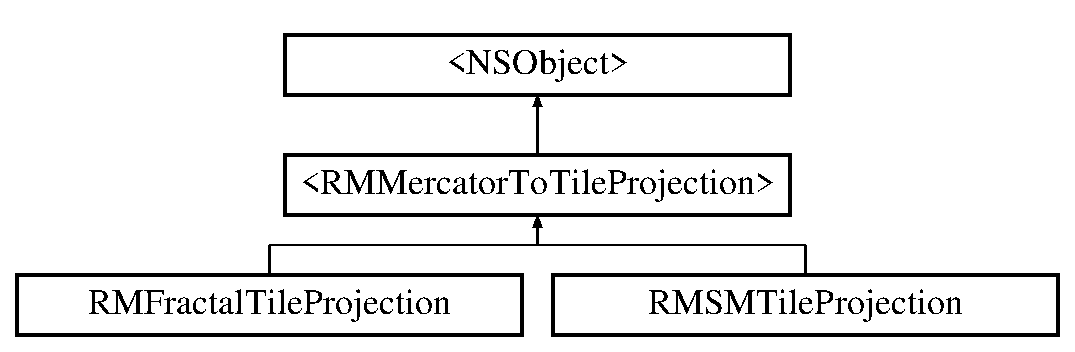
\includegraphics[height=3.000000cm]{protocol_r_m_mercator_to_tile_projection-p}
\end{center}
\end{figure}
\subsection*{Instance Methods}
\begin{DoxyCompactItemize}
\item 
(float) -\/ \hyperlink{protocol_r_m_mercator_to_tile_projection-p_a470b0ea952dd174bbd573bdfb230cc6e}{calculate\-Normalised\-Zoom\-From\-Scale\-:}
\item 
(float) -\/ \hyperlink{protocol_r_m_mercator_to_tile_projection-p_a49c836acfac1908808c5f218f3bc64a4}{calculate\-Scale\-From\-Zoom\-:}
\item 
(float) -\/ \hyperlink{protocol_r_m_mercator_to_tile_projection-p_a013a65cf254c34e3ec021864a4fb8f53}{calculate\-Zoom\-From\-Scale\-:}
\item 
(\hyperlink{struct_r_m_tile}{R\-M\-Tile}) -\/ \hyperlink{protocol_r_m_mercator_to_tile_projection-p_ac8776965edc17be3e90c03aad46a8371}{normalise\-Tile\-:}
\item 
(float) -\/ \hyperlink{protocol_r_m_mercator_to_tile_projection-p_a48d47f3689db59a82bde9da209529f9b}{normalise\-Zoom\-:}
\item 
(\hyperlink{struct_r_m_tile_rect}{R\-M\-Tile\-Rect}) -\/ \hyperlink{protocol_r_m_mercator_to_tile_projection-p_ae80633ea6d0b4e354666ec6e7ddd88af}{project\-:}
\begin{DoxyCompactList}\small\item\em This is a helper for project\-Rect above. Much simpler for the caller. \end{DoxyCompactList}\item 
(\hyperlink{struct_r_m_tile_point}{R\-M\-Tile\-Point}) -\/ \hyperlink{protocol_r_m_mercator_to_tile_projection-p_aac47d8222bec29f9d8469d166510b9cd}{project\-:at\-Scale\-:}
\item 
(\hyperlink{struct_r_m_tile_point}{R\-M\-Tile\-Point}) -\/ \hyperlink{protocol_r_m_mercator_to_tile_projection-p_a0351c94bf59dfc97b5c1c712a5b2f3b2}{project\-:at\-Zoom\-:}
\item 
(\hyperlink{struct_r_m_tile_rect}{R\-M\-Tile\-Rect}) -\/ \hyperlink{protocol_r_m_mercator_to_tile_projection-p_a6d26aef35f64a793066fdf8c4e3cda10}{project\-Rect\-:at\-Scale\-:}
\item 
(\hyperlink{struct_r_m_tile_rect}{R\-M\-Tile\-Rect}) -\/ \hyperlink{protocol_r_m_mercator_to_tile_projection-p_a53c5b90994528d20a3d85307244ac412}{project\-Rect\-:at\-Zoom\-:}
\end{DoxyCompactItemize}
\subsection*{属性}
\begin{DoxyCompactItemize}
\item 
N\-S\-U\-Integer \hyperlink{protocol_r_m_mercator_to_tile_projection-p_ae98173b5589ce9707510ee13a5bd6a23}{max\-Zoom}
\begin{DoxyCompactList}\small\item\em Maximum zoom for which we have tile images. \end{DoxyCompactList}\item 
N\-S\-U\-Integer \hyperlink{protocol_r_m_mercator_to_tile_projection-p_a3db7c10c5566330cdd76e97519f87f6e}{min\-Zoom}
\begin{DoxyCompactList}\small\item\em Minimum zoom for which we have tile images. \end{DoxyCompactList}\item 
\hyperlink{struct_r_m_projected_rect}{R\-M\-Projected\-Rect} \hyperlink{protocol_r_m_mercator_to_tile_projection-p_a5bb487ce4d5c60437bc63dd355371bfd}{planet\-Bounds}
\begin{DoxyCompactList}\small\item\em bounds of the earth, in projected units (meters). \end{DoxyCompactList}\item 
N\-S\-U\-Integer \hyperlink{protocol_r_m_mercator_to_tile_projection-p_a9e7426ca0ae5a5375822f500a49cd829}{tile\-Side\-Length}
\begin{DoxyCompactList}\small\item\em Tile side length in pixels. \end{DoxyCompactList}\end{DoxyCompactItemize}


\subsection{详细描述}
A tile projection is a projection which turns mercators into tile coordinates. 

At time of writing, read \hyperlink{interface_r_m_fractal_tile_projection}{R\-M\-Fractal\-Tile\-Projection} to see the implementation of this. 

\subsection{Method Documentation}
\hypertarget{protocol_r_m_mercator_to_tile_projection-p_a470b0ea952dd174bbd573bdfb230cc6e}{\index{R\-M\-Mercator\-To\-Tile\-Projection-\/p@{R\-M\-Mercator\-To\-Tile\-Projection-\/p}!calculate\-Normalised\-Zoom\-From\-Scale\-:@{calculate\-Normalised\-Zoom\-From\-Scale\-:}}
\index{calculate\-Normalised\-Zoom\-From\-Scale\-:@{calculate\-Normalised\-Zoom\-From\-Scale\-:}!RMMercatorToTileProjection-p@{R\-M\-Mercator\-To\-Tile\-Projection-\/p}}
\subsubsection[{calculate\-Normalised\-Zoom\-From\-Scale\-:}]{\setlength{\rightskip}{0pt plus 5cm}-\/ (float) calculate\-Normalised\-Zoom\-From\-Scale\-: 
\begin{DoxyParamCaption}
\item[{(float)}]{scale}
\end{DoxyParamCaption}
}}\label{protocol_r_m_mercator_to_tile_projection-p_a470b0ea952dd174bbd573bdfb230cc6e}


被 \hyperlink{interface_r_m_fractal_tile_projection_a6432f229f4cfabfba65b7b702d0eb96c}{R\-M\-Fractal\-Tile\-Projection} , 以及 \hyperlink{interface_r_m_s_m_tile_projection_aba4de218e94a607507926e279e149a7a}{R\-M\-S\-M\-Tile\-Projection} 重载.

\hypertarget{protocol_r_m_mercator_to_tile_projection-p_a49c836acfac1908808c5f218f3bc64a4}{\index{R\-M\-Mercator\-To\-Tile\-Projection-\/p@{R\-M\-Mercator\-To\-Tile\-Projection-\/p}!calculate\-Scale\-From\-Zoom\-:@{calculate\-Scale\-From\-Zoom\-:}}
\index{calculate\-Scale\-From\-Zoom\-:@{calculate\-Scale\-From\-Zoom\-:}!RMMercatorToTileProjection-p@{R\-M\-Mercator\-To\-Tile\-Projection-\/p}}
\subsubsection[{calculate\-Scale\-From\-Zoom\-:}]{\setlength{\rightskip}{0pt plus 5cm}-\/ (float) calculate\-Scale\-From\-Zoom\-: 
\begin{DoxyParamCaption}
\item[{(float)}]{zoom}
\end{DoxyParamCaption}
}}\label{protocol_r_m_mercator_to_tile_projection-p_a49c836acfac1908808c5f218f3bc64a4}


被 \hyperlink{interface_r_m_fractal_tile_projection_aea5d9c0bdb2b6eb460d9882d6b2a46ec}{R\-M\-Fractal\-Tile\-Projection} , 以及 \hyperlink{interface_r_m_s_m_tile_projection_a94301528cc8b93a91910b955bc149946}{R\-M\-S\-M\-Tile\-Projection} 重载.

\hypertarget{protocol_r_m_mercator_to_tile_projection-p_a013a65cf254c34e3ec021864a4fb8f53}{\index{R\-M\-Mercator\-To\-Tile\-Projection-\/p@{R\-M\-Mercator\-To\-Tile\-Projection-\/p}!calculate\-Zoom\-From\-Scale\-:@{calculate\-Zoom\-From\-Scale\-:}}
\index{calculate\-Zoom\-From\-Scale\-:@{calculate\-Zoom\-From\-Scale\-:}!RMMercatorToTileProjection-p@{R\-M\-Mercator\-To\-Tile\-Projection-\/p}}
\subsubsection[{calculate\-Zoom\-From\-Scale\-:}]{\setlength{\rightskip}{0pt plus 5cm}-\/ (float) calculate\-Zoom\-From\-Scale\-: 
\begin{DoxyParamCaption}
\item[{(float)}]{scale}
\end{DoxyParamCaption}
}}\label{protocol_r_m_mercator_to_tile_projection-p_a013a65cf254c34e3ec021864a4fb8f53}


被 \hyperlink{interface_r_m_fractal_tile_projection_a8604a8779fd50182367c0b176bd5a2ec}{R\-M\-Fractal\-Tile\-Projection} , 以及 \hyperlink{interface_r_m_s_m_tile_projection_abec26590a653146faa9faa3dcc26faf9}{R\-M\-S\-M\-Tile\-Projection} 重载.

\hypertarget{protocol_r_m_mercator_to_tile_projection-p_ac8776965edc17be3e90c03aad46a8371}{\index{R\-M\-Mercator\-To\-Tile\-Projection-\/p@{R\-M\-Mercator\-To\-Tile\-Projection-\/p}!normalise\-Tile\-:@{normalise\-Tile\-:}}
\index{normalise\-Tile\-:@{normalise\-Tile\-:}!RMMercatorToTileProjection-p@{R\-M\-Mercator\-To\-Tile\-Projection-\/p}}
\subsubsection[{normalise\-Tile\-:}]{\setlength{\rightskip}{0pt plus 5cm}-\/ ({\bf R\-M\-Tile}) normalise\-Tile\-: 
\begin{DoxyParamCaption}
\item[{({\bf R\-M\-Tile})}]{tile}
\end{DoxyParamCaption}
}}\label{protocol_r_m_mercator_to_tile_projection-p_ac8776965edc17be3e90c03aad46a8371}


被 \hyperlink{interface_r_m_fractal_tile_projection_a6ab9f21ef545dbac3647001f64022335}{R\-M\-Fractal\-Tile\-Projection} , 以及 \hyperlink{interface_r_m_s_m_tile_projection_afb0bc6d1a3c82c27cf704689e9afb349}{R\-M\-S\-M\-Tile\-Projection} 重载.

\hypertarget{protocol_r_m_mercator_to_tile_projection-p_a48d47f3689db59a82bde9da209529f9b}{\index{R\-M\-Mercator\-To\-Tile\-Projection-\/p@{R\-M\-Mercator\-To\-Tile\-Projection-\/p}!normalise\-Zoom\-:@{normalise\-Zoom\-:}}
\index{normalise\-Zoom\-:@{normalise\-Zoom\-:}!RMMercatorToTileProjection-p@{R\-M\-Mercator\-To\-Tile\-Projection-\/p}}
\subsubsection[{normalise\-Zoom\-:}]{\setlength{\rightskip}{0pt plus 5cm}-\/ (float) normalise\-Zoom\-: 
\begin{DoxyParamCaption}
\item[{(float)}]{zoom}
\end{DoxyParamCaption}
}}\label{protocol_r_m_mercator_to_tile_projection-p_a48d47f3689db59a82bde9da209529f9b}


被 \hyperlink{interface_r_m_fractal_tile_projection_a08e53c12b44631258e909dbc33385c96}{R\-M\-Fractal\-Tile\-Projection} , 以及 \hyperlink{interface_r_m_s_m_tile_projection_a36e33099f7112bc3a9e2a6d899f31763}{R\-M\-S\-M\-Tile\-Projection} 重载.

\hypertarget{protocol_r_m_mercator_to_tile_projection-p_ae80633ea6d0b4e354666ec6e7ddd88af}{\index{R\-M\-Mercator\-To\-Tile\-Projection-\/p@{R\-M\-Mercator\-To\-Tile\-Projection-\/p}!project\-:@{project\-:}}
\index{project\-:@{project\-:}!RMMercatorToTileProjection-p@{R\-M\-Mercator\-To\-Tile\-Projection-\/p}}
\subsubsection[{project\-:}]{\setlength{\rightskip}{0pt plus 5cm}-\/ ({\bf R\-M\-Tile\-Rect}) project\-: 
\begin{DoxyParamCaption}
\item[{({\bf R\-M\-Mercator\-To\-Screen\-Projection} $\ast$)}]{screen}
\end{DoxyParamCaption}
}}\label{protocol_r_m_mercator_to_tile_projection-p_ae80633ea6d0b4e354666ec6e7ddd88af}


This is a helper for project\-Rect above. Much simpler for the caller. 



被 \hyperlink{interface_r_m_fractal_tile_projection_a76f6d1fea39a1c577ff0b26012b05c9c}{R\-M\-Fractal\-Tile\-Projection} , 以及 \hyperlink{interface_r_m_s_m_tile_projection_a5a6e55b1fd17c79125d4d5fe7db20284}{R\-M\-S\-M\-Tile\-Projection} 重载.

\hypertarget{protocol_r_m_mercator_to_tile_projection-p_aac47d8222bec29f9d8469d166510b9cd}{\index{R\-M\-Mercator\-To\-Tile\-Projection-\/p@{R\-M\-Mercator\-To\-Tile\-Projection-\/p}!project\-:at\-Scale\-:@{project\-:at\-Scale\-:}}
\index{project\-:at\-Scale\-:@{project\-:at\-Scale\-:}!RMMercatorToTileProjection-p@{R\-M\-Mercator\-To\-Tile\-Projection-\/p}}
\subsubsection[{project\-:at\-Scale\-:}]{\setlength{\rightskip}{0pt plus 5cm}-\/ ({\bf R\-M\-Tile\-Point}) {\bf project\-:} 
\begin{DoxyParamCaption}
\item[{({\bf R\-M\-Projected\-Point})}]{a\-Point}
\item[{atScale:(float)}]{scale}
\end{DoxyParamCaption}
}}\label{protocol_r_m_mercator_to_tile_projection-p_aac47d8222bec29f9d8469d166510b9cd}


被 \hyperlink{interface_r_m_fractal_tile_projection_a794c40f61be19f6efcb23e95a45ab1b4}{R\-M\-Fractal\-Tile\-Projection} , 以及 \hyperlink{interface_r_m_s_m_tile_projection_a0ff895767233e8f338247faa3b2bee1f}{R\-M\-S\-M\-Tile\-Projection} 重载.

\hypertarget{protocol_r_m_mercator_to_tile_projection-p_a0351c94bf59dfc97b5c1c712a5b2f3b2}{\index{R\-M\-Mercator\-To\-Tile\-Projection-\/p@{R\-M\-Mercator\-To\-Tile\-Projection-\/p}!project\-:at\-Zoom\-:@{project\-:at\-Zoom\-:}}
\index{project\-:at\-Zoom\-:@{project\-:at\-Zoom\-:}!RMMercatorToTileProjection-p@{R\-M\-Mercator\-To\-Tile\-Projection-\/p}}
\subsubsection[{project\-:at\-Zoom\-:}]{\setlength{\rightskip}{0pt plus 5cm}-\/ ({\bf R\-M\-Tile\-Point}) {\bf project\-:} 
\begin{DoxyParamCaption}
\item[{({\bf R\-M\-Projected\-Point})}]{a\-Point}
\item[{atZoom:(float)}]{zoom}
\end{DoxyParamCaption}
}}\label{protocol_r_m_mercator_to_tile_projection-p_a0351c94bf59dfc97b5c1c712a5b2f3b2}


被 \hyperlink{interface_r_m_fractal_tile_projection_afff85793493770d6424965f65c5690f7}{R\-M\-Fractal\-Tile\-Projection} , 以及 \hyperlink{interface_r_m_s_m_tile_projection_a27b45f6348b6b10d0ac808a8ee6b6c97}{R\-M\-S\-M\-Tile\-Projection} 重载.

\hypertarget{protocol_r_m_mercator_to_tile_projection-p_a6d26aef35f64a793066fdf8c4e3cda10}{\index{R\-M\-Mercator\-To\-Tile\-Projection-\/p@{R\-M\-Mercator\-To\-Tile\-Projection-\/p}!project\-Rect\-:at\-Scale\-:@{project\-Rect\-:at\-Scale\-:}}
\index{project\-Rect\-:at\-Scale\-:@{project\-Rect\-:at\-Scale\-:}!RMMercatorToTileProjection-p@{R\-M\-Mercator\-To\-Tile\-Projection-\/p}}
\subsubsection[{project\-Rect\-:at\-Scale\-:}]{\setlength{\rightskip}{0pt plus 5cm}-\/ ({\bf R\-M\-Tile\-Rect}) project\-Rect\-: 
\begin{DoxyParamCaption}
\item[{({\bf R\-M\-Projected\-Rect})}]{a\-Rect}
\item[{atScale:(float)}]{scale}
\end{DoxyParamCaption}
}}\label{protocol_r_m_mercator_to_tile_projection-p_a6d26aef35f64a793066fdf8c4e3cda10}


被 \hyperlink{interface_r_m_fractal_tile_projection_aca623bc1c542e85df15c30cfd2233b88}{R\-M\-Fractal\-Tile\-Projection} , 以及 \hyperlink{interface_r_m_s_m_tile_projection_a69ee12f033da79ab6f088fb8ca11fbfd}{R\-M\-S\-M\-Tile\-Projection} 重载.

\hypertarget{protocol_r_m_mercator_to_tile_projection-p_a53c5b90994528d20a3d85307244ac412}{\index{R\-M\-Mercator\-To\-Tile\-Projection-\/p@{R\-M\-Mercator\-To\-Tile\-Projection-\/p}!project\-Rect\-:at\-Zoom\-:@{project\-Rect\-:at\-Zoom\-:}}
\index{project\-Rect\-:at\-Zoom\-:@{project\-Rect\-:at\-Zoom\-:}!RMMercatorToTileProjection-p@{R\-M\-Mercator\-To\-Tile\-Projection-\/p}}
\subsubsection[{project\-Rect\-:at\-Zoom\-:}]{\setlength{\rightskip}{0pt plus 5cm}-\/ ({\bf R\-M\-Tile\-Rect}) project\-Rect\-: 
\begin{DoxyParamCaption}
\item[{({\bf R\-M\-Projected\-Rect})}]{a\-Rect}
\item[{atZoom:(float)}]{zoom}
\end{DoxyParamCaption}
}}\label{protocol_r_m_mercator_to_tile_projection-p_a53c5b90994528d20a3d85307244ac412}


被 \hyperlink{interface_r_m_fractal_tile_projection_abd518c9cae2d4440be0d00be14dff12b}{R\-M\-Fractal\-Tile\-Projection} , 以及 \hyperlink{interface_r_m_s_m_tile_projection_a8442a53b7624d621ab15d9027b48b7e9}{R\-M\-S\-M\-Tile\-Projection} 重载.



\subsection{属性说明}
\hypertarget{protocol_r_m_mercator_to_tile_projection-p_ae98173b5589ce9707510ee13a5bd6a23}{\index{R\-M\-Mercator\-To\-Tile\-Projection-\/p@{R\-M\-Mercator\-To\-Tile\-Projection-\/p}!max\-Zoom@{max\-Zoom}}
\index{max\-Zoom@{max\-Zoom}!RMMercatorToTileProjection-p@{R\-M\-Mercator\-To\-Tile\-Projection-\/p}}
\subsubsection[{max\-Zoom}]{\setlength{\rightskip}{0pt plus 5cm}-\/ (N\-S\-U\-Integer) max\-Zoom\hspace{0.3cm}{\ttfamily [read]}, {\ttfamily [nonatomic]}, {\ttfamily [assign]}}}\label{protocol_r_m_mercator_to_tile_projection-p_ae98173b5589ce9707510ee13a5bd6a23}


Maximum zoom for which we have tile images. 

\hypertarget{protocol_r_m_mercator_to_tile_projection-p_a3db7c10c5566330cdd76e97519f87f6e}{\index{R\-M\-Mercator\-To\-Tile\-Projection-\/p@{R\-M\-Mercator\-To\-Tile\-Projection-\/p}!min\-Zoom@{min\-Zoom}}
\index{min\-Zoom@{min\-Zoom}!RMMercatorToTileProjection-p@{R\-M\-Mercator\-To\-Tile\-Projection-\/p}}
\subsubsection[{min\-Zoom}]{\setlength{\rightskip}{0pt plus 5cm}-\/ (N\-S\-U\-Integer) min\-Zoom\hspace{0.3cm}{\ttfamily [read]}, {\ttfamily [nonatomic]}, {\ttfamily [assign]}}}\label{protocol_r_m_mercator_to_tile_projection-p_a3db7c10c5566330cdd76e97519f87f6e}


Minimum zoom for which we have tile images. 

\hypertarget{protocol_r_m_mercator_to_tile_projection-p_a5bb487ce4d5c60437bc63dd355371bfd}{\index{R\-M\-Mercator\-To\-Tile\-Projection-\/p@{R\-M\-Mercator\-To\-Tile\-Projection-\/p}!planet\-Bounds@{planet\-Bounds}}
\index{planet\-Bounds@{planet\-Bounds}!RMMercatorToTileProjection-p@{R\-M\-Mercator\-To\-Tile\-Projection-\/p}}
\subsubsection[{planet\-Bounds}]{\setlength{\rightskip}{0pt plus 5cm}-\/ ({\bf R\-M\-Projected\-Rect}) planet\-Bounds\hspace{0.3cm}{\ttfamily [read]}, {\ttfamily [nonatomic]}, {\ttfamily [assign]}}}\label{protocol_r_m_mercator_to_tile_projection-p_a5bb487ce4d5c60437bc63dd355371bfd}


bounds of the earth, in projected units (meters). 

\hypertarget{protocol_r_m_mercator_to_tile_projection-p_a9e7426ca0ae5a5375822f500a49cd829}{\index{R\-M\-Mercator\-To\-Tile\-Projection-\/p@{R\-M\-Mercator\-To\-Tile\-Projection-\/p}!tile\-Side\-Length@{tile\-Side\-Length}}
\index{tile\-Side\-Length@{tile\-Side\-Length}!RMMercatorToTileProjection-p@{R\-M\-Mercator\-To\-Tile\-Projection-\/p}}
\subsubsection[{tile\-Side\-Length}]{\setlength{\rightskip}{0pt plus 5cm}-\/ (N\-S\-U\-Integer) tile\-Side\-Length\hspace{0.3cm}{\ttfamily [read]}, {\ttfamily [nonatomic]}, {\ttfamily [assign]}}}\label{protocol_r_m_mercator_to_tile_projection-p_a9e7426ca0ae5a5375822f500a49cd829}


Tile side length in pixels. 



该协议的文档由以下文件生成\-:\begin{DoxyCompactItemize}
\item 
Map/\hyperlink{_r_m_mercator_to_tile_projection_8h}{R\-M\-Mercator\-To\-Tile\-Projection.\-h}\end{DoxyCompactItemize}

\hypertarget{protocol_r_m_moving_map_layer-p}{\section{$<$R\-M\-Moving\-Map\-Layer$>$协议 参考}
\label{protocol_r_m_moving_map_layer-p}\index{$<$\-R\-M\-Moving\-Map\-Layer$>$@{$<$\-R\-M\-Moving\-Map\-Layer$>$}}
}


{\ttfamily \#import $<$R\-M\-Map\-Layer.\-h$>$}

类 $<$R\-M\-Moving\-Map\-Layer$>$ 继承关系图\-:\begin{figure}[H]
\begin{center}
\leavevmode
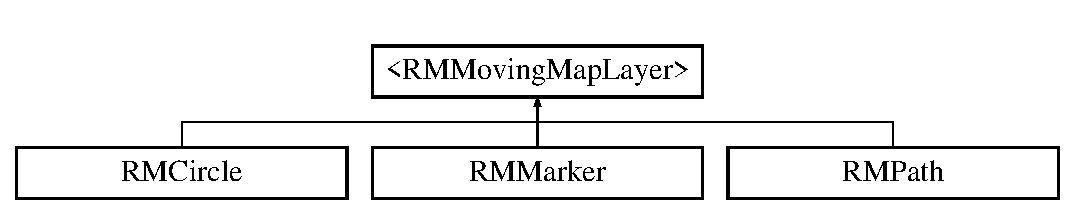
\includegraphics[height=2.000000cm]{protocol_r_m_moving_map_layer-p}
\end{center}
\end{figure}
\subsection*{属性}
\begin{DoxyCompactItemize}
\item 
B\-O\-O\-L \hyperlink{protocol_r_m_moving_map_layer-p_a5ee0b003170b8e66e2ac6bf4ea8820be}{enable\-Dragging}
\item 
B\-O\-O\-L \hyperlink{protocol_r_m_moving_map_layer-p_ada91bd4f9f5507b894d1534c01727ee9}{enable\-Rotation}
\item 
\hyperlink{struct_r_m_projected_point}{R\-M\-Projected\-Point} \hyperlink{protocol_r_m_moving_map_layer-p_a4a6ac55816966cfafc82a6e5114d2cac}{projected\-Location}
\end{DoxyCompactItemize}


\subsection{属性说明}
\hypertarget{protocol_r_m_moving_map_layer-p_a5ee0b003170b8e66e2ac6bf4ea8820be}{\index{R\-M\-Moving\-Map\-Layer-\/p@{R\-M\-Moving\-Map\-Layer-\/p}!enable\-Dragging@{enable\-Dragging}}
\index{enable\-Dragging@{enable\-Dragging}!RMMovingMapLayer-p@{R\-M\-Moving\-Map\-Layer-\/p}}
\subsubsection[{enable\-Dragging}]{\setlength{\rightskip}{0pt plus 5cm}-\/ (B\-O\-O\-L) enable\-Dragging\hspace{0.3cm}{\ttfamily [read]}, {\ttfamily [write]}, {\ttfamily [atomic]}, {\ttfamily [assign]}}}\label{protocol_r_m_moving_map_layer-p_a5ee0b003170b8e66e2ac6bf4ea8820be}
\hypertarget{protocol_r_m_moving_map_layer-p_ada91bd4f9f5507b894d1534c01727ee9}{\index{R\-M\-Moving\-Map\-Layer-\/p@{R\-M\-Moving\-Map\-Layer-\/p}!enable\-Rotation@{enable\-Rotation}}
\index{enable\-Rotation@{enable\-Rotation}!RMMovingMapLayer-p@{R\-M\-Moving\-Map\-Layer-\/p}}
\subsubsection[{enable\-Rotation}]{\setlength{\rightskip}{0pt plus 5cm}-\/ (B\-O\-O\-L) enable\-Rotation\hspace{0.3cm}{\ttfamily [read]}, {\ttfamily [write]}, {\ttfamily [atomic]}, {\ttfamily [assign]}}}\label{protocol_r_m_moving_map_layer-p_ada91bd4f9f5507b894d1534c01727ee9}
\hypertarget{protocol_r_m_moving_map_layer-p_a4a6ac55816966cfafc82a6e5114d2cac}{\index{R\-M\-Moving\-Map\-Layer-\/p@{R\-M\-Moving\-Map\-Layer-\/p}!projected\-Location@{projected\-Location}}
\index{projected\-Location@{projected\-Location}!RMMovingMapLayer-p@{R\-M\-Moving\-Map\-Layer-\/p}}
\subsubsection[{projected\-Location}]{\setlength{\rightskip}{0pt plus 5cm}-\/ ({\bf R\-M\-Projected\-Point}) projected\-Location\hspace{0.3cm}{\ttfamily [read]}, {\ttfamily [write]}, {\ttfamily [nonatomic]}, {\ttfamily [assign]}}}\label{protocol_r_m_moving_map_layer-p_a4a6ac55816966cfafc82a6e5114d2cac}


该协议的文档由以下文件生成\-:\begin{DoxyCompactItemize}
\item 
Map/\hyperlink{_r_m_map_layer_8h}{R\-M\-Map\-Layer.\-h}\end{DoxyCompactItemize}

\hypertarget{interface_r_m_open_aerial_map_source}{\section{R\-M\-Open\-Aerial\-Map\-Source类 参考}
\label{interface_r_m_open_aerial_map_source}\index{R\-M\-Open\-Aerial\-Map\-Source@{R\-M\-Open\-Aerial\-Map\-Source}}
}


Subclass of \hyperlink{interface_r_m_abstract_mercator_web_source}{R\-M\-Abstract\-Mercator\-Web\-Source} for access to the Open Aerial Map project's development server.  




{\ttfamily \#import $<$R\-M\-Open\-Aerial\-Map\-Source.\-h$>$}

类 R\-M\-Open\-Aerial\-Map\-Source 继承关系图\-:\begin{figure}[H]
\begin{center}
\leavevmode
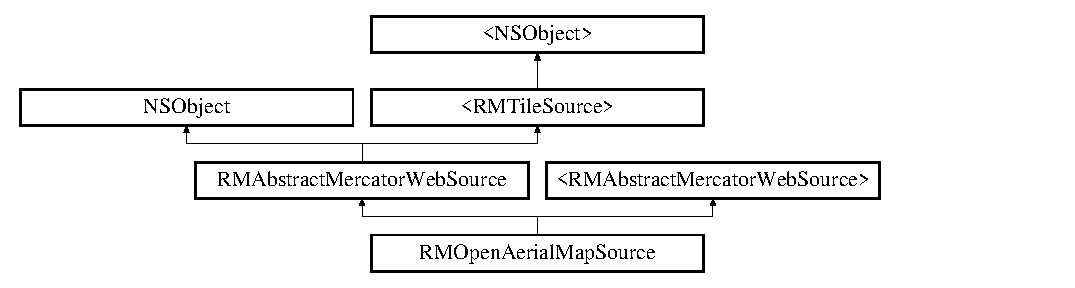
\includegraphics[height=3.425076cm]{interface_r_m_open_aerial_map_source}
\end{center}
\end{figure}
\subsection*{Instance Methods}
\begin{DoxyCompactItemize}
\item 
(id) -\/ \hyperlink{interface_r_m_open_aerial_map_source_a05c9a3ffef1c399e854f0aaaa252924e}{init}{\ttfamily  \mbox{[}implementation\mbox{]}}
\item 
(N\-S\-String $\ast$) -\/ \hyperlink{interface_r_m_open_aerial_map_source_a3ee5ed718434f321be5ad57fe4c527b8}{long\-Attribution}{\ttfamily  \mbox{[}implementation\mbox{]}}
\item 
(N\-S\-String $\ast$) -\/ \hyperlink{interface_r_m_open_aerial_map_source_a52f16e426510e04e68da57baa32e0a23}{long\-Description}{\ttfamily  \mbox{[}implementation\mbox{]}}
\item 
(N\-S\-String $\ast$) -\/ \hyperlink{interface_r_m_open_aerial_map_source_ac20a79118d42831a77a162d4e42f3309}{short\-Attribution}{\ttfamily  \mbox{[}implementation\mbox{]}}
\item 
(N\-S\-String $\ast$) -\/ \hyperlink{interface_r_m_open_aerial_map_source_aeee53f47d6b8e07c9db69a200e13738e}{short\-Name}{\ttfamily  \mbox{[}implementation\mbox{]}}
\item 
(N\-S\-String $\ast$) -\/ \hyperlink{interface_r_m_open_aerial_map_source_a4405601eb40cc53cf9d2f2875acc2be2}{tile\-U\-R\-L\-:}{\ttfamily  \mbox{[}implementation\mbox{]}}
\item 
(N\-S\-String $\ast$) -\/ \hyperlink{interface_r_m_open_aerial_map_source_a5da92a4a64ec3e3ecb36068b5264ca3f}{unique\-Tilecache\-Key}{\ttfamily  \mbox{[}implementation\mbox{]}}
\end{DoxyCompactItemize}
\subsection*{额外继承的成员函数}


\subsection{详细描述}
Subclass of \hyperlink{interface_r_m_abstract_mercator_web_source}{R\-M\-Abstract\-Mercator\-Web\-Source} for access to the Open Aerial Map project's development server. 

Provides access to tiles from the Open Aerial Map project. 

\subsection{Method Documentation}
\hypertarget{interface_r_m_open_aerial_map_source_a05c9a3ffef1c399e854f0aaaa252924e}{\index{R\-M\-Open\-Aerial\-Map\-Source@{R\-M\-Open\-Aerial\-Map\-Source}!init@{init}}
\index{init@{init}!RMOpenAerialMapSource@{R\-M\-Open\-Aerial\-Map\-Source}}
\subsubsection[{init}]{\setlength{\rightskip}{0pt plus 5cm}-\/ (id) init 
\begin{DoxyParamCaption}
{}
\end{DoxyParamCaption}
\hspace{0.3cm}{\ttfamily [implementation]}}}\label{interface_r_m_open_aerial_map_source_a05c9a3ffef1c399e854f0aaaa252924e}


重载 \hyperlink{interface_r_m_abstract_mercator_web_source_a88bc1ea00a789381d77ae50e0eaec732}{R\-M\-Abstract\-Mercator\-Web\-Source} .

\hypertarget{interface_r_m_open_aerial_map_source_a3ee5ed718434f321be5ad57fe4c527b8}{\index{R\-M\-Open\-Aerial\-Map\-Source@{R\-M\-Open\-Aerial\-Map\-Source}!long\-Attribution@{long\-Attribution}}
\index{long\-Attribution@{long\-Attribution}!RMOpenAerialMapSource@{R\-M\-Open\-Aerial\-Map\-Source}}
\subsubsection[{long\-Attribution}]{\setlength{\rightskip}{0pt plus 5cm}-\/ (N\-S\-String $\ast$) long\-Attribution 
\begin{DoxyParamCaption}
{}
\end{DoxyParamCaption}
\hspace{0.3cm}{\ttfamily [implementation]}}}\label{interface_r_m_open_aerial_map_source_a3ee5ed718434f321be5ad57fe4c527b8}


重载 \hyperlink{interface_r_m_abstract_mercator_web_source_a77313c2d697428dd994a6e0cf07a256f}{R\-M\-Abstract\-Mercator\-Web\-Source} .

\hypertarget{interface_r_m_open_aerial_map_source_a52f16e426510e04e68da57baa32e0a23}{\index{R\-M\-Open\-Aerial\-Map\-Source@{R\-M\-Open\-Aerial\-Map\-Source}!long\-Description@{long\-Description}}
\index{long\-Description@{long\-Description}!RMOpenAerialMapSource@{R\-M\-Open\-Aerial\-Map\-Source}}
\subsubsection[{long\-Description}]{\setlength{\rightskip}{0pt plus 5cm}-\/ (N\-S\-String $\ast$) long\-Description 
\begin{DoxyParamCaption}
{}
\end{DoxyParamCaption}
\hspace{0.3cm}{\ttfamily [implementation]}}}\label{interface_r_m_open_aerial_map_source_a52f16e426510e04e68da57baa32e0a23}


重载 \hyperlink{interface_r_m_abstract_mercator_web_source_a9c1c86280c6fa05e4e82502822fcfd10}{R\-M\-Abstract\-Mercator\-Web\-Source} .

\hypertarget{interface_r_m_open_aerial_map_source_ac20a79118d42831a77a162d4e42f3309}{\index{R\-M\-Open\-Aerial\-Map\-Source@{R\-M\-Open\-Aerial\-Map\-Source}!short\-Attribution@{short\-Attribution}}
\index{short\-Attribution@{short\-Attribution}!RMOpenAerialMapSource@{R\-M\-Open\-Aerial\-Map\-Source}}
\subsubsection[{short\-Attribution}]{\setlength{\rightskip}{0pt plus 5cm}-\/ (N\-S\-String $\ast$) short\-Attribution 
\begin{DoxyParamCaption}
{}
\end{DoxyParamCaption}
\hspace{0.3cm}{\ttfamily [implementation]}}}\label{interface_r_m_open_aerial_map_source_ac20a79118d42831a77a162d4e42f3309}


重载 \hyperlink{interface_r_m_abstract_mercator_web_source_a6be24cea169d058b5eefd7572bedc366}{R\-M\-Abstract\-Mercator\-Web\-Source} .

\hypertarget{interface_r_m_open_aerial_map_source_aeee53f47d6b8e07c9db69a200e13738e}{\index{R\-M\-Open\-Aerial\-Map\-Source@{R\-M\-Open\-Aerial\-Map\-Source}!short\-Name@{short\-Name}}
\index{short\-Name@{short\-Name}!RMOpenAerialMapSource@{R\-M\-Open\-Aerial\-Map\-Source}}
\subsubsection[{short\-Name}]{\setlength{\rightskip}{0pt plus 5cm}-\/ (N\-S\-String $\ast$) short\-Name 
\begin{DoxyParamCaption}
{}
\end{DoxyParamCaption}
\hspace{0.3cm}{\ttfamily [implementation]}}}\label{interface_r_m_open_aerial_map_source_aeee53f47d6b8e07c9db69a200e13738e}


重载 \hyperlink{interface_r_m_abstract_mercator_web_source_a3e6c6ef18250ce14317373db9df1fc85}{R\-M\-Abstract\-Mercator\-Web\-Source} .

\hypertarget{interface_r_m_open_aerial_map_source_a4405601eb40cc53cf9d2f2875acc2be2}{\index{R\-M\-Open\-Aerial\-Map\-Source@{R\-M\-Open\-Aerial\-Map\-Source}!tile\-U\-R\-L\-:@{tile\-U\-R\-L\-:}}
\index{tile\-U\-R\-L\-:@{tile\-U\-R\-L\-:}!RMOpenAerialMapSource@{R\-M\-Open\-Aerial\-Map\-Source}}
\subsubsection[{tile\-U\-R\-L\-:}]{\setlength{\rightskip}{0pt plus 5cm}-\/ (N\-S\-String $\ast$) tile\-U\-R\-L\-: 
\begin{DoxyParamCaption}
\item[{({\bf R\-M\-Tile})}]{tile}
\end{DoxyParamCaption}
\hspace{0.3cm}{\ttfamily [implementation]}}}\label{interface_r_m_open_aerial_map_source_a4405601eb40cc53cf9d2f2875acc2be2}


重载 \hyperlink{protocol_r_m_abstract_mercator_web_source-p_ae5c62f0fed7dcdfd78aa9582bdec9b4b}{$<$\-R\-M\-Abstract\-Mercator\-Web\-Source$>$} .

\hypertarget{interface_r_m_open_aerial_map_source_a5da92a4a64ec3e3ecb36068b5264ca3f}{\index{R\-M\-Open\-Aerial\-Map\-Source@{R\-M\-Open\-Aerial\-Map\-Source}!unique\-Tilecache\-Key@{unique\-Tilecache\-Key}}
\index{unique\-Tilecache\-Key@{unique\-Tilecache\-Key}!RMOpenAerialMapSource@{R\-M\-Open\-Aerial\-Map\-Source}}
\subsubsection[{unique\-Tilecache\-Key}]{\setlength{\rightskip}{0pt plus 5cm}-\/ (N\-S\-String $\ast$) unique\-Tilecache\-Key 
\begin{DoxyParamCaption}
{}
\end{DoxyParamCaption}
\hspace{0.3cm}{\ttfamily [implementation]}}}\label{interface_r_m_open_aerial_map_source_a5da92a4a64ec3e3ecb36068b5264ca3f}


重载 \hyperlink{interface_r_m_abstract_mercator_web_source_acf45b84d8f39ef7fcc2a92a2e320a9a2}{R\-M\-Abstract\-Mercator\-Web\-Source} .



该类的文档由以下文件生成\-:\begin{DoxyCompactItemize}
\item 
Map/\hyperlink{_r_m_open_aerial_map_source_8h}{R\-M\-Open\-Aerial\-Map\-Source.\-h}\item 
Map/\hyperlink{_r_m_open_aerial_map_source_8m}{R\-M\-Open\-Aerial\-Map\-Source.\-m}\end{DoxyCompactItemize}

\hypertarget{interface_r_m_open_cycle_map_source}{\section{R\-M\-Open\-Cycle\-Map\-Source类 参考}
\label{interface_r_m_open_cycle_map_source}\index{R\-M\-Open\-Cycle\-Map\-Source@{R\-M\-Open\-Cycle\-Map\-Source}}
}


Subclass of \hyperlink{interface_r_m_abstract_mercator_web_source}{R\-M\-Abstract\-Mercator\-Web\-Source} for access to the Open Cycle Map project's development server.  




{\ttfamily \#import $<$R\-M\-Open\-Cycle\-Map\-Source.\-h$>$}

类 R\-M\-Open\-Cycle\-Map\-Source 继承关系图\-:\begin{figure}[H]
\begin{center}
\leavevmode
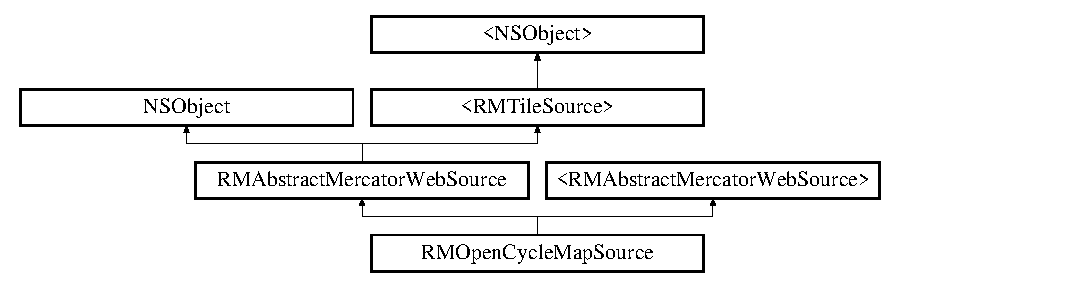
\includegraphics[height=3.425076cm]{interface_r_m_open_cycle_map_source}
\end{center}
\end{figure}
\subsection*{Instance Methods}
\begin{DoxyCompactItemize}
\item 
(id) -\/ \hyperlink{interface_r_m_open_cycle_map_source_a44641fcc78a286cb2deb35124e260165}{init}{\ttfamily  \mbox{[}implementation\mbox{]}}
\item 
(N\-S\-String $\ast$) -\/ \hyperlink{interface_r_m_open_cycle_map_source_af84dc5628aac3458972ab37a9364dd4d}{long\-Attribution}{\ttfamily  \mbox{[}implementation\mbox{]}}
\item 
(N\-S\-String $\ast$) -\/ \hyperlink{interface_r_m_open_cycle_map_source_a3d30e39f50df22cf3ddba68ae4eda864}{long\-Description}{\ttfamily  \mbox{[}implementation\mbox{]}}
\item 
(N\-S\-String $\ast$) -\/ \hyperlink{interface_r_m_open_cycle_map_source_a3c0c39e8ab0896390bd329e75e55860e}{short\-Attribution}{\ttfamily  \mbox{[}implementation\mbox{]}}
\item 
(N\-S\-String $\ast$) -\/ \hyperlink{interface_r_m_open_cycle_map_source_ac9b00e3fbdde801fdda353681d05d838}{short\-Name}{\ttfamily  \mbox{[}implementation\mbox{]}}
\item 
(N\-S\-String $\ast$) -\/ \hyperlink{interface_r_m_open_cycle_map_source_a65f5b088a340d5b0e519a244f4f549fd}{tile\-U\-R\-L\-:}{\ttfamily  \mbox{[}implementation\mbox{]}}
\item 
(N\-S\-String $\ast$) -\/ \hyperlink{interface_r_m_open_cycle_map_source_a8f454702038372b215a4cfabdce76022}{unique\-Tilecache\-Key}{\ttfamily  \mbox{[}implementation\mbox{]}}
\end{DoxyCompactItemize}
\subsection*{额外继承的成员函数}


\subsection{详细描述}
Subclass of \hyperlink{interface_r_m_abstract_mercator_web_source}{R\-M\-Abstract\-Mercator\-Web\-Source} for access to the Open Cycle Map project's development server. 

Provides key-\/based access to tiles from the Open Cycle Map project. 

\subsection{Method Documentation}
\hypertarget{interface_r_m_open_cycle_map_source_a44641fcc78a286cb2deb35124e260165}{\index{R\-M\-Open\-Cycle\-Map\-Source@{R\-M\-Open\-Cycle\-Map\-Source}!init@{init}}
\index{init@{init}!RMOpenCycleMapSource@{R\-M\-Open\-Cycle\-Map\-Source}}
\subsubsection[{init}]{\setlength{\rightskip}{0pt plus 5cm}-\/ (id) init 
\begin{DoxyParamCaption}
{}
\end{DoxyParamCaption}
\hspace{0.3cm}{\ttfamily [implementation]}}}\label{interface_r_m_open_cycle_map_source_a44641fcc78a286cb2deb35124e260165}


重载 \hyperlink{interface_r_m_abstract_mercator_web_source_a88bc1ea00a789381d77ae50e0eaec732}{R\-M\-Abstract\-Mercator\-Web\-Source} .

\hypertarget{interface_r_m_open_cycle_map_source_af84dc5628aac3458972ab37a9364dd4d}{\index{R\-M\-Open\-Cycle\-Map\-Source@{R\-M\-Open\-Cycle\-Map\-Source}!long\-Attribution@{long\-Attribution}}
\index{long\-Attribution@{long\-Attribution}!RMOpenCycleMapSource@{R\-M\-Open\-Cycle\-Map\-Source}}
\subsubsection[{long\-Attribution}]{\setlength{\rightskip}{0pt plus 5cm}-\/ (N\-S\-String $\ast$) long\-Attribution 
\begin{DoxyParamCaption}
{}
\end{DoxyParamCaption}
\hspace{0.3cm}{\ttfamily [implementation]}}}\label{interface_r_m_open_cycle_map_source_af84dc5628aac3458972ab37a9364dd4d}


重载 \hyperlink{interface_r_m_abstract_mercator_web_source_a77313c2d697428dd994a6e0cf07a256f}{R\-M\-Abstract\-Mercator\-Web\-Source} .

\hypertarget{interface_r_m_open_cycle_map_source_a3d30e39f50df22cf3ddba68ae4eda864}{\index{R\-M\-Open\-Cycle\-Map\-Source@{R\-M\-Open\-Cycle\-Map\-Source}!long\-Description@{long\-Description}}
\index{long\-Description@{long\-Description}!RMOpenCycleMapSource@{R\-M\-Open\-Cycle\-Map\-Source}}
\subsubsection[{long\-Description}]{\setlength{\rightskip}{0pt plus 5cm}-\/ (N\-S\-String $\ast$) long\-Description 
\begin{DoxyParamCaption}
{}
\end{DoxyParamCaption}
\hspace{0.3cm}{\ttfamily [implementation]}}}\label{interface_r_m_open_cycle_map_source_a3d30e39f50df22cf3ddba68ae4eda864}


重载 \hyperlink{interface_r_m_abstract_mercator_web_source_a9c1c86280c6fa05e4e82502822fcfd10}{R\-M\-Abstract\-Mercator\-Web\-Source} .

\hypertarget{interface_r_m_open_cycle_map_source_a3c0c39e8ab0896390bd329e75e55860e}{\index{R\-M\-Open\-Cycle\-Map\-Source@{R\-M\-Open\-Cycle\-Map\-Source}!short\-Attribution@{short\-Attribution}}
\index{short\-Attribution@{short\-Attribution}!RMOpenCycleMapSource@{R\-M\-Open\-Cycle\-Map\-Source}}
\subsubsection[{short\-Attribution}]{\setlength{\rightskip}{0pt plus 5cm}-\/ (N\-S\-String $\ast$) short\-Attribution 
\begin{DoxyParamCaption}
{}
\end{DoxyParamCaption}
\hspace{0.3cm}{\ttfamily [implementation]}}}\label{interface_r_m_open_cycle_map_source_a3c0c39e8ab0896390bd329e75e55860e}


重载 \hyperlink{interface_r_m_abstract_mercator_web_source_a6be24cea169d058b5eefd7572bedc366}{R\-M\-Abstract\-Mercator\-Web\-Source} .

\hypertarget{interface_r_m_open_cycle_map_source_ac9b00e3fbdde801fdda353681d05d838}{\index{R\-M\-Open\-Cycle\-Map\-Source@{R\-M\-Open\-Cycle\-Map\-Source}!short\-Name@{short\-Name}}
\index{short\-Name@{short\-Name}!RMOpenCycleMapSource@{R\-M\-Open\-Cycle\-Map\-Source}}
\subsubsection[{short\-Name}]{\setlength{\rightskip}{0pt plus 5cm}-\/ (N\-S\-String $\ast$) short\-Name 
\begin{DoxyParamCaption}
{}
\end{DoxyParamCaption}
\hspace{0.3cm}{\ttfamily [implementation]}}}\label{interface_r_m_open_cycle_map_source_ac9b00e3fbdde801fdda353681d05d838}


重载 \hyperlink{interface_r_m_abstract_mercator_web_source_a3e6c6ef18250ce14317373db9df1fc85}{R\-M\-Abstract\-Mercator\-Web\-Source} .

\hypertarget{interface_r_m_open_cycle_map_source_a65f5b088a340d5b0e519a244f4f549fd}{\index{R\-M\-Open\-Cycle\-Map\-Source@{R\-M\-Open\-Cycle\-Map\-Source}!tile\-U\-R\-L\-:@{tile\-U\-R\-L\-:}}
\index{tile\-U\-R\-L\-:@{tile\-U\-R\-L\-:}!RMOpenCycleMapSource@{R\-M\-Open\-Cycle\-Map\-Source}}
\subsubsection[{tile\-U\-R\-L\-:}]{\setlength{\rightskip}{0pt plus 5cm}-\/ (N\-S\-String $\ast$) tile\-U\-R\-L\-: 
\begin{DoxyParamCaption}
\item[{({\bf R\-M\-Tile})}]{tile}
\end{DoxyParamCaption}
\hspace{0.3cm}{\ttfamily [implementation]}}}\label{interface_r_m_open_cycle_map_source_a65f5b088a340d5b0e519a244f4f549fd}


重载 \hyperlink{protocol_r_m_abstract_mercator_web_source-p_ae5c62f0fed7dcdfd78aa9582bdec9b4b}{$<$\-R\-M\-Abstract\-Mercator\-Web\-Source$>$} .

\hypertarget{interface_r_m_open_cycle_map_source_a8f454702038372b215a4cfabdce76022}{\index{R\-M\-Open\-Cycle\-Map\-Source@{R\-M\-Open\-Cycle\-Map\-Source}!unique\-Tilecache\-Key@{unique\-Tilecache\-Key}}
\index{unique\-Tilecache\-Key@{unique\-Tilecache\-Key}!RMOpenCycleMapSource@{R\-M\-Open\-Cycle\-Map\-Source}}
\subsubsection[{unique\-Tilecache\-Key}]{\setlength{\rightskip}{0pt plus 5cm}-\/ (N\-S\-String $\ast$) unique\-Tilecache\-Key 
\begin{DoxyParamCaption}
{}
\end{DoxyParamCaption}
\hspace{0.3cm}{\ttfamily [implementation]}}}\label{interface_r_m_open_cycle_map_source_a8f454702038372b215a4cfabdce76022}


重载 \hyperlink{interface_r_m_abstract_mercator_web_source_acf45b84d8f39ef7fcc2a92a2e320a9a2}{R\-M\-Abstract\-Mercator\-Web\-Source} .



该类的文档由以下文件生成\-:\begin{DoxyCompactItemize}
\item 
Map/\hyperlink{_r_m_open_cycle_map_source_8h}{R\-M\-Open\-Cycle\-Map\-Source.\-h}\item 
Map/\hyperlink{_r_m_open_cycle_map_source_8m}{R\-M\-Open\-Cycle\-Map\-Source.\-m}\end{DoxyCompactItemize}

\hypertarget{interface_r_m_open_street_map_source}{\section{R\-M\-Open\-Street\-Map\-Source类 参考}
\label{interface_r_m_open_street_map_source}\index{R\-M\-Open\-Street\-Map\-Source@{R\-M\-Open\-Street\-Map\-Source}}
}


Subclass of \hyperlink{interface_r_m_abstract_mercator_web_source}{R\-M\-Abstract\-Mercator\-Web\-Source} for access to the Open Street Map project's development server.  




{\ttfamily \#import $<$R\-M\-Open\-Street\-Map\-Source.\-h$>$}

类 R\-M\-Open\-Street\-Map\-Source 继承关系图\-:\begin{figure}[H]
\begin{center}
\leavevmode
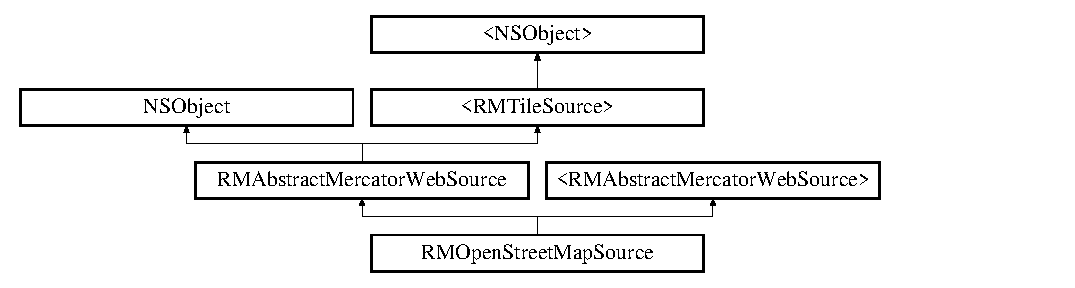
\includegraphics[height=3.425076cm]{interface_r_m_open_street_map_source}
\end{center}
\end{figure}
\subsection*{Instance Methods}
\begin{DoxyCompactItemize}
\item 
(id) -\/ \hyperlink{interface_r_m_open_street_map_source_ad2c425f72e1d6342eb533a64426c1ecc}{init}{\ttfamily  \mbox{[}implementation\mbox{]}}
\item 
(N\-S\-String $\ast$) -\/ \hyperlink{interface_r_m_open_street_map_source_a932b3f4e2d2015eaadae1e5876f3fd14}{long\-Attribution}{\ttfamily  \mbox{[}implementation\mbox{]}}
\item 
(N\-S\-String $\ast$) -\/ \hyperlink{interface_r_m_open_street_map_source_acf8470afa308a44db7eab70e1366c570}{long\-Description}{\ttfamily  \mbox{[}implementation\mbox{]}}
\item 
(N\-S\-String $\ast$) -\/ \hyperlink{interface_r_m_open_street_map_source_a9ff8d53d553a5fd3e091a1dec5d720fe}{short\-Attribution}{\ttfamily  \mbox{[}implementation\mbox{]}}
\item 
(N\-S\-String $\ast$) -\/ \hyperlink{interface_r_m_open_street_map_source_a2c36d88b3653099053eb46129a245a55}{short\-Name}{\ttfamily  \mbox{[}implementation\mbox{]}}
\item 
(N\-S\-String $\ast$) -\/ \hyperlink{interface_r_m_open_street_map_source_a3d2b2c15f17ca1ab3d1862ffb1feb2e3}{tile\-U\-R\-L\-:}{\ttfamily  \mbox{[}implementation\mbox{]}}
\item 
(N\-S\-String $\ast$) -\/ \hyperlink{interface_r_m_open_street_map_source_a6bf79a7fd62c28cb11979a7d4bdb65b9}{unique\-Tilecache\-Key}{\ttfamily  \mbox{[}implementation\mbox{]}}
\end{DoxyCompactItemize}
\subsection*{额外继承的成员函数}


\subsection{详细描述}
Subclass of \hyperlink{interface_r_m_abstract_mercator_web_source}{R\-M\-Abstract\-Mercator\-Web\-Source} for access to the Open Street Map project's development server. 

Provides key-\/based access to tiles from the Open Street Map project. 

\subsection{Method Documentation}
\hypertarget{interface_r_m_open_street_map_source_ad2c425f72e1d6342eb533a64426c1ecc}{\index{R\-M\-Open\-Street\-Map\-Source@{R\-M\-Open\-Street\-Map\-Source}!init@{init}}
\index{init@{init}!RMOpenStreetMapSource@{R\-M\-Open\-Street\-Map\-Source}}
\subsubsection[{init}]{\setlength{\rightskip}{0pt plus 5cm}-\/ (id) init 
\begin{DoxyParamCaption}
{}
\end{DoxyParamCaption}
\hspace{0.3cm}{\ttfamily [implementation]}}}\label{interface_r_m_open_street_map_source_ad2c425f72e1d6342eb533a64426c1ecc}


重载 \hyperlink{interface_r_m_abstract_mercator_web_source_a88bc1ea00a789381d77ae50e0eaec732}{R\-M\-Abstract\-Mercator\-Web\-Source} .

\hypertarget{interface_r_m_open_street_map_source_a932b3f4e2d2015eaadae1e5876f3fd14}{\index{R\-M\-Open\-Street\-Map\-Source@{R\-M\-Open\-Street\-Map\-Source}!long\-Attribution@{long\-Attribution}}
\index{long\-Attribution@{long\-Attribution}!RMOpenStreetMapSource@{R\-M\-Open\-Street\-Map\-Source}}
\subsubsection[{long\-Attribution}]{\setlength{\rightskip}{0pt plus 5cm}-\/ (N\-S\-String $\ast$) long\-Attribution 
\begin{DoxyParamCaption}
{}
\end{DoxyParamCaption}
\hspace{0.3cm}{\ttfamily [implementation]}}}\label{interface_r_m_open_street_map_source_a932b3f4e2d2015eaadae1e5876f3fd14}


重载 \hyperlink{interface_r_m_abstract_mercator_web_source_a77313c2d697428dd994a6e0cf07a256f}{R\-M\-Abstract\-Mercator\-Web\-Source} .

\hypertarget{interface_r_m_open_street_map_source_acf8470afa308a44db7eab70e1366c570}{\index{R\-M\-Open\-Street\-Map\-Source@{R\-M\-Open\-Street\-Map\-Source}!long\-Description@{long\-Description}}
\index{long\-Description@{long\-Description}!RMOpenStreetMapSource@{R\-M\-Open\-Street\-Map\-Source}}
\subsubsection[{long\-Description}]{\setlength{\rightskip}{0pt plus 5cm}-\/ (N\-S\-String $\ast$) long\-Description 
\begin{DoxyParamCaption}
{}
\end{DoxyParamCaption}
\hspace{0.3cm}{\ttfamily [implementation]}}}\label{interface_r_m_open_street_map_source_acf8470afa308a44db7eab70e1366c570}


重载 \hyperlink{interface_r_m_abstract_mercator_web_source_a9c1c86280c6fa05e4e82502822fcfd10}{R\-M\-Abstract\-Mercator\-Web\-Source} .

\hypertarget{interface_r_m_open_street_map_source_a9ff8d53d553a5fd3e091a1dec5d720fe}{\index{R\-M\-Open\-Street\-Map\-Source@{R\-M\-Open\-Street\-Map\-Source}!short\-Attribution@{short\-Attribution}}
\index{short\-Attribution@{short\-Attribution}!RMOpenStreetMapSource@{R\-M\-Open\-Street\-Map\-Source}}
\subsubsection[{short\-Attribution}]{\setlength{\rightskip}{0pt plus 5cm}-\/ (N\-S\-String $\ast$) short\-Attribution 
\begin{DoxyParamCaption}
{}
\end{DoxyParamCaption}
\hspace{0.3cm}{\ttfamily [implementation]}}}\label{interface_r_m_open_street_map_source_a9ff8d53d553a5fd3e091a1dec5d720fe}


重载 \hyperlink{interface_r_m_abstract_mercator_web_source_a6be24cea169d058b5eefd7572bedc366}{R\-M\-Abstract\-Mercator\-Web\-Source} .

\hypertarget{interface_r_m_open_street_map_source_a2c36d88b3653099053eb46129a245a55}{\index{R\-M\-Open\-Street\-Map\-Source@{R\-M\-Open\-Street\-Map\-Source}!short\-Name@{short\-Name}}
\index{short\-Name@{short\-Name}!RMOpenStreetMapSource@{R\-M\-Open\-Street\-Map\-Source}}
\subsubsection[{short\-Name}]{\setlength{\rightskip}{0pt plus 5cm}-\/ (N\-S\-String $\ast$) short\-Name 
\begin{DoxyParamCaption}
{}
\end{DoxyParamCaption}
\hspace{0.3cm}{\ttfamily [implementation]}}}\label{interface_r_m_open_street_map_source_a2c36d88b3653099053eb46129a245a55}


重载 \hyperlink{interface_r_m_abstract_mercator_web_source_a3e6c6ef18250ce14317373db9df1fc85}{R\-M\-Abstract\-Mercator\-Web\-Source} .

\hypertarget{interface_r_m_open_street_map_source_a3d2b2c15f17ca1ab3d1862ffb1feb2e3}{\index{R\-M\-Open\-Street\-Map\-Source@{R\-M\-Open\-Street\-Map\-Source}!tile\-U\-R\-L\-:@{tile\-U\-R\-L\-:}}
\index{tile\-U\-R\-L\-:@{tile\-U\-R\-L\-:}!RMOpenStreetMapSource@{R\-M\-Open\-Street\-Map\-Source}}
\subsubsection[{tile\-U\-R\-L\-:}]{\setlength{\rightskip}{0pt plus 5cm}-\/ (N\-S\-String $\ast$) tile\-U\-R\-L\-: 
\begin{DoxyParamCaption}
\item[{({\bf R\-M\-Tile})}]{tile}
\end{DoxyParamCaption}
\hspace{0.3cm}{\ttfamily [implementation]}}}\label{interface_r_m_open_street_map_source_a3d2b2c15f17ca1ab3d1862ffb1feb2e3}


重载 \hyperlink{protocol_r_m_abstract_mercator_web_source-p_ae5c62f0fed7dcdfd78aa9582bdec9b4b}{$<$\-R\-M\-Abstract\-Mercator\-Web\-Source$>$} .

\hypertarget{interface_r_m_open_street_map_source_a6bf79a7fd62c28cb11979a7d4bdb65b9}{\index{R\-M\-Open\-Street\-Map\-Source@{R\-M\-Open\-Street\-Map\-Source}!unique\-Tilecache\-Key@{unique\-Tilecache\-Key}}
\index{unique\-Tilecache\-Key@{unique\-Tilecache\-Key}!RMOpenStreetMapSource@{R\-M\-Open\-Street\-Map\-Source}}
\subsubsection[{unique\-Tilecache\-Key}]{\setlength{\rightskip}{0pt plus 5cm}-\/ (N\-S\-String $\ast$) unique\-Tilecache\-Key 
\begin{DoxyParamCaption}
{}
\end{DoxyParamCaption}
\hspace{0.3cm}{\ttfamily [implementation]}}}\label{interface_r_m_open_street_map_source_a6bf79a7fd62c28cb11979a7d4bdb65b9}


重载 \hyperlink{interface_r_m_abstract_mercator_web_source_acf45b84d8f39ef7fcc2a92a2e320a9a2}{R\-M\-Abstract\-Mercator\-Web\-Source} .



该类的文档由以下文件生成\-:\begin{DoxyCompactItemize}
\item 
Map/\hyperlink{_r_m_open_street_map_source_8h}{R\-M\-Open\-Street\-Map\-Source.\-h}\item 
Map/\hyperlink{_r_m_open_street_map_source_8m}{R\-M\-Open\-Street\-Map\-Source.\-m}\end{DoxyCompactItemize}

\hypertarget{interface_r_m_path}{\section{R\-M\-Path类 参考}
\label{interface_r_m_path}\index{R\-M\-Path@{R\-M\-Path}}
}


{\ttfamily \#import $<$R\-M\-Path.\-h$>$}

类 R\-M\-Path 继承关系图\-:\begin{figure}[H]
\begin{center}
\leavevmode
\includegraphics[height=3.000000cm]{interface_r_m_path}
\end{center}
\end{figure}
\subsection*{Instance Methods}
\begin{DoxyCompactItemize}
\item 
(id$<$ C\-A\-Action $>$) -\/ \hyperlink{interface_r_m_path_aeff4f90d5d01092fd310a0b52d3c9d1c}{action\-For\-Key\-:}{\ttfamily  \mbox{[}implementation\mbox{]}}
\item 
(void) -\/ \hyperlink{interface_r_m_path_a233d38ded11a78015f57d9aee26e8c42}{add\-Line\-To\-Lat\-Long\-:}
\item 
(void) -\/ \hyperlink{interface_r_m_path_a9635a32a6026e63fdf1b34b243dd1d08}{add\-Line\-To\-Screen\-Point\-:}
\item 
(void) -\/ \hyperlink{interface_r_m_path_ac05f8be482e0aa0e3050247d5143f356}{add\-Line\-To\-X\-Y\-:}
\item 
(void) -\/ \hyperlink{interface_r_m_path_a63d207d98b22f4a77875fdf8d18b7ed5}{add\-Point\-To\-X\-Y\-:with\-Drawing\-:}{\ttfamily  \mbox{[}implementation\mbox{]}}
\item 
(void) -\/ \hyperlink{interface_r_m_path_acfcc36a04919726a503d9d692c365f3d}{close\-Path}
\item 
(void) -\/ \hyperlink{interface_r_m_path_a4b50da18017f5fc9530ff05401747da0}{dealloc}{\ttfamily  \mbox{[}implementation\mbox{]}}
\item 
(void) -\/ \hyperlink{interface_r_m_path_a4c02b41834cd9435a62bb2db42eff620}{draw\-In\-Context\-:}{\ttfamily  \mbox{[}implementation\mbox{]}}
\item 
(id) -\/ \hyperlink{interface_r_m_path_a29187a042475bad3699856e3385bb3ee}{init\-For\-Map\-:}
\item 
(id) -\/ \hyperlink{interface_r_m_path_acf830718a51227db7bebef87f58af3fa}{init\-For\-Map\-:with\-Coordinates\-:count\-:}
\item 
(id) -\/ \hyperlink{interface_r_m_path_af79f1923ee9c26625021fe3952076858}{init\-With\-Contents\-:}
\item 
(void) -\/ \hyperlink{interface_r_m_path_aa51fa75ed859403de65279c357720646}{move\-By\-:}{\ttfamily  \mbox{[}implementation\mbox{]}}
\item 
(void) -\/ \hyperlink{interface_r_m_path_a9dc844ebe9a05ba48a0ff601b7621684}{move\-To\-Lat\-Long\-:}
\item 
(void) -\/ \hyperlink{interface_r_m_path_a76134695ca29b3d58857a5d100a8db61}{move\-To\-Screen\-Point\-:}
\item 
(void) -\/ \hyperlink{interface_r_m_path_a8152252d92f15d9a64ced43b242e75f3}{move\-To\-X\-Y\-:}
\item 
(void) -\/ \hyperlink{interface_r_m_path_a49d02bb5a66b86321ef003a2e82fdaa4}{recalculate\-Geometry}{\ttfamily  \mbox{[}implementation\mbox{]}}
\item 
(void) -\/ \hyperlink{interface_r_m_path_adcebd60bb2931ac35682cd98663df01b}{resume\-Expensive\-Operations\-Notification\-:}{\ttfamily  \mbox{[}implementation\mbox{]}}
\item 
(void) -\/ \hyperlink{interface_r_m_path_a9dbaa031097817f66fb60a08b0152f03}{set\-Fill\-Color\-:}{\ttfamily  \mbox{[}implementation\mbox{]}}
\item 
(void) -\/ \hyperlink{interface_r_m_path_a26399b883723e767df48cc65103f49ef}{set\-Line\-Cap\-:}{\ttfamily  \mbox{[}implementation\mbox{]}}
\item 
(void) -\/ \hyperlink{interface_r_m_path_a1189f1035fce44a2cd33a7ec908ff6eb}{set\-Line\-Color\-:}{\ttfamily  \mbox{[}implementation\mbox{]}}
\item 
(void) -\/ \hyperlink{interface_r_m_path_aac24db1aea9ae5f3fbe07d4689d9b6e6}{set\-Line\-Dash\-Lengths\-:}{\ttfamily  \mbox{[}implementation\mbox{]}}
\item 
(void) -\/ \hyperlink{interface_r_m_path_aae7dd8305cb31482013fc9572c2b008e}{set\-Line\-Join\-:}{\ttfamily  \mbox{[}implementation\mbox{]}}
\item 
(void) -\/ \hyperlink{interface_r_m_path_a0e41e0d279a6be9e9560a391bfa4ed4a}{set\-Line\-Width\-:}{\ttfamily  \mbox{[}implementation\mbox{]}}
\item 
(void) -\/ \hyperlink{interface_r_m_path_a3594420667f2f8e13093716cb9e26a80}{set\-Position\-:}{\ttfamily  \mbox{[}implementation\mbox{]}}
\item 
(void) -\/ \hyperlink{interface_r_m_path_a8a39a0577a19fc38e05e64cbd3c233a5}{set\-Shadow\-Blur\-:}{\ttfamily  \mbox{[}implementation\mbox{]}}
\item 
(void) -\/ \hyperlink{interface_r_m_path_ab795b2187b18ee2397beb1945db1f4e3}{set\-Shadow\-Color\-:}{\ttfamily  \mbox{[}implementation\mbox{]}}
\item 
(void) -\/ \hyperlink{interface_r_m_path_a457d78db2535206b5c9c1653623e151f}{set\-Shadow\-Offset\-:}{\ttfamily  \mbox{[}implementation\mbox{]}}
\end{DoxyCompactItemize}
\subsection*{Protected 属性}
\begin{DoxyCompactItemize}
\item 
size\-\_\-t \hyperlink{interface_r_m_path_ad3e04fb162632bb0b1a16e73e566ca21}{\-\_\-line\-Dash\-Count}
\item 
C\-G\-Float $\ast$ \hyperlink{interface_r_m_path_acf58af65bc4c356e2ef1944810801d13}{\-\_\-line\-Dash\-Lengths}
\item 
C\-G\-Float $\ast$ \hyperlink{interface_r_m_path_aa91685824ea8a4e4d69c76bb64712fc0}{\-\_\-scaled\-Line\-Dash\-Lengths}
\item 
\hyperlink{interface_r_m_map_contents}{R\-M\-Map\-Contents} $\ast$ \hyperlink{interface_r_m_path_ad95b46462e03361c8dd1793ed93358bf}{map\-Contents}
\item 
int \hyperlink{interface_r_m_path_a7c6712af40b4154351635f68812b001c}{n\-Temp\-Parts}
\item 
C\-G\-Rect \hyperlink{interface_r_m_path_a94e057a30ec95a4d5b29d32db112ed68}{original\-Contents\-Rect}
\item 
C\-G\-Mutable\-Path\-Ref \hyperlink{interface_r_m_path_ae603ad2b9d405ea3eed4639f5fff4cd7}{path}
\item 
B\-O\-O\-L \hyperlink{interface_r_m_path_a01f6bb4208525cf246b68cdf8f6bf510}{redraw\-Pending}
\end{DoxyCompactItemize}
\subsection*{属性}
\begin{DoxyCompactItemize}
\item 
B\-O\-O\-L \hyperlink{interface_r_m_path_a5e0cdd3cfdf9f079c87555b21e3a8c6e}{b\-Is\-Close\-Path}
\item 
C\-G\-Path\-Ref \hyperlink{interface_r_m_path_af8606a78ec0d3c5994f95b6e5b5b1fd4}{C\-G\-Path}
\item 
B\-O\-O\-L \hyperlink{interface_r_m_path_a6a67c253aa7d8b01eb220c8bcfd9e82f}{enable\-Dragging}
\item 
B\-O\-O\-L \hyperlink{interface_r_m_path_a2ee8138aeba736c62e3025c1d4d6cfde}{enable\-Rotation}
\item 
U\-I\-Color $\ast$ \hyperlink{interface_r_m_path_a24c78845b1cad7d0a707719958a6999e}{fill\-Color}
\item 
C\-G\-Line\-Cap \hyperlink{interface_r_m_path_af0b6eebd8bc03615b3ac8981d05eabef}{line\-Cap}
\item 
U\-I\-Color $\ast$ \hyperlink{interface_r_m_path_ae8b3e91ec89a67481bead38e350e57d7}{line\-Color}
\item 
N\-S\-Array $\ast$ \hyperlink{interface_r_m_path_ae3cb38856ea7fadfab64a740056404ea}{line\-Dash\-Lengths}
\item 
C\-G\-Float \hyperlink{interface_r_m_path_a0280407af3e1d6d0b665af9d2d40ee2d}{line\-Dash\-Phase}
\item 
C\-G\-Line\-Join \hyperlink{interface_r_m_path_a0418ed1c257890ec76454022b32a1077}{line\-Join}
\item 
float \hyperlink{interface_r_m_path_afe3c2bce6675d281fc86f60923b7b8e5}{line\-Width}
\item 
N\-S\-Mutable\-Array $\ast$ \hyperlink{interface_r_m_path_a1e478ab9621bef7d287b13accde96514}{parts}
\item 
N\-S\-Mutable\-Array $\ast$ \hyperlink{interface_r_m_path_a376fb33189a4b9f1f6694825fc7d77d4}{points}
\item 
\hyperlink{struct_r_m_projected_rect}{R\-M\-Projected\-Rect} \hyperlink{interface_r_m_path_ab57ac16906ba51dfc400d02f6a6cce0d}{projected\-Bounds}
\item 
\hyperlink{struct_r_m_projected_point}{R\-M\-Projected\-Point} \hyperlink{interface_r_m_path_a696f7378ed70695bdbc0257105e48eda}{projected\-Location}
\item 
B\-O\-O\-L \hyperlink{interface_r_m_path_afccc6b38950cc3acd53faf1deca80a20}{scale\-Line\-Dash}
\item 
B\-O\-O\-L \hyperlink{interface_r_m_path_a5736a6c5b238f1b928bdfd0659bc9093}{scale\-Line\-Width}
\item 
C\-G\-Float \hyperlink{interface_r_m_path_ac6266f68f5c8dc01aa913e5a74f8ac11}{shadow\-Blur}
\item 
U\-I\-Color $\ast$ \hyperlink{interface_r_m_path_a2478b26b83164f11d71b5c716c733c34}{shadow\-Color}
\item 
C\-G\-Size \hyperlink{interface_r_m_path_ad0a770fb5c74fc7bb09b2d15a642fac5}{shadow\-Offset}
\end{DoxyCompactItemize}


\subsection{Method Documentation}
\hypertarget{interface_r_m_path_aeff4f90d5d01092fd310a0b52d3c9d1c}{\index{R\-M\-Path@{R\-M\-Path}!action\-For\-Key\-:@{action\-For\-Key\-:}}
\index{action\-For\-Key\-:@{action\-For\-Key\-:}!RMPath@{R\-M\-Path}}
\subsubsection[{action\-For\-Key\-:}]{\setlength{\rightskip}{0pt plus 5cm}-\/ (id$<$ C\-A\-Action $>$) action\-For\-Key\-: 
\begin{DoxyParamCaption}
\item[{(N\-S\-String $\ast$)}]{key}
\end{DoxyParamCaption}
\hspace{0.3cm}{\ttfamily [implementation]}}}\label{interface_r_m_path_aeff4f90d5d01092fd310a0b52d3c9d1c}
\begin{DoxyRefDesc}{Bug}
\item[\hyperlink{bug__bug000018}{Bug}]why return nil for the \char`\"{}position\char`\"{} and \char`\"{}bounds\char`\"{} action\-For\-Key? Does this do anything besides block Core Animation? \end{DoxyRefDesc}


重载 \hyperlink{interface_r_m_map_layer_a28e0dabc0cf8638c6d26358354f4fcf8}{R\-M\-Map\-Layer} .

\hypertarget{interface_r_m_path_a233d38ded11a78015f57d9aee26e8c42}{\index{R\-M\-Path@{R\-M\-Path}!add\-Line\-To\-Lat\-Long\-:@{add\-Line\-To\-Lat\-Long\-:}}
\index{add\-Line\-To\-Lat\-Long\-:@{add\-Line\-To\-Lat\-Long\-:}!RMPath@{R\-M\-Path}}
\subsubsection[{add\-Line\-To\-Lat\-Long\-:}]{\setlength{\rightskip}{0pt plus 5cm}-\/ (void) add\-Line\-To\-Lat\-Long\-: 
\begin{DoxyParamCaption}
\item[{({\bf R\-M\-Lat\-Long})}]{point}
\end{DoxyParamCaption}
}}\label{interface_r_m_path_a233d38ded11a78015f57d9aee26e8c42}


参考自 init\-For\-Map\-:with\-Coordinates\-:count\-: , 以及 Server\-Geometry\-::to\-R\-M\-Path\-:.

\hypertarget{interface_r_m_path_a9635a32a6026e63fdf1b34b243dd1d08}{\index{R\-M\-Path@{R\-M\-Path}!add\-Line\-To\-Screen\-Point\-:@{add\-Line\-To\-Screen\-Point\-:}}
\index{add\-Line\-To\-Screen\-Point\-:@{add\-Line\-To\-Screen\-Point\-:}!RMPath@{R\-M\-Path}}
\subsubsection[{add\-Line\-To\-Screen\-Point\-:}]{\setlength{\rightskip}{0pt plus 5cm}-\/ (void) add\-Line\-To\-Screen\-Point\-: 
\begin{DoxyParamCaption}
\item[{(C\-G\-Point)}]{point}
\end{DoxyParamCaption}
}}\label{interface_r_m_path_a9635a32a6026e63fdf1b34b243dd1d08}
\hypertarget{interface_r_m_path_ac05f8be482e0aa0e3050247d5143f356}{\index{R\-M\-Path@{R\-M\-Path}!add\-Line\-To\-X\-Y\-:@{add\-Line\-To\-X\-Y\-:}}
\index{add\-Line\-To\-X\-Y\-:@{add\-Line\-To\-X\-Y\-:}!RMPath@{R\-M\-Path}}
\subsubsection[{add\-Line\-To\-X\-Y\-:}]{\setlength{\rightskip}{0pt plus 5cm}-\/ (void) add\-Line\-To\-X\-Y\-: 
\begin{DoxyParamCaption}
\item[{({\bf R\-M\-Projected\-Point})}]{point}
\end{DoxyParamCaption}
}}\label{interface_r_m_path_ac05f8be482e0aa0e3050247d5143f356}


参考自 add\-Line\-To\-Lat\-Long\-: , 以及 add\-Line\-To\-Screen\-Point\-:.

\hypertarget{interface_r_m_path_a63d207d98b22f4a77875fdf8d18b7ed5}{\index{R\-M\-Path@{R\-M\-Path}!add\-Point\-To\-X\-Y\-:with\-Drawing\-:@{add\-Point\-To\-X\-Y\-:with\-Drawing\-:}}
\index{add\-Point\-To\-X\-Y\-:with\-Drawing\-:@{add\-Point\-To\-X\-Y\-:with\-Drawing\-:}!RMPath@{R\-M\-Path}}
\subsubsection[{add\-Point\-To\-X\-Y\-:with\-Drawing\-:}]{\setlength{\rightskip}{0pt plus 5cm}-\/ (void) add\-Point\-To\-X\-Y\-: 
\begin{DoxyParamCaption}
\item[{({\bf R\-M\-Projected\-Point})}]{point}
\item[{withDrawing:(B\-O\-O\-L)}]{is\-Drawing}
\end{DoxyParamCaption}
\hspace{0.3cm}{\ttfamily [implementation]}}}\label{interface_r_m_path_a63d207d98b22f4a77875fdf8d18b7ed5}


参考自 add\-Line\-To\-X\-Y\-: , 以及 move\-To\-X\-Y\-:.

\hypertarget{interface_r_m_path_acfcc36a04919726a503d9d692c365f3d}{\index{R\-M\-Path@{R\-M\-Path}!close\-Path@{close\-Path}}
\index{close\-Path@{close\-Path}!RMPath@{R\-M\-Path}}
\subsubsection[{close\-Path}]{\setlength{\rightskip}{0pt plus 5cm}-\/ (void) close\-Path 
\begin{DoxyParamCaption}
{}
\end{DoxyParamCaption}
}}\label{interface_r_m_path_acfcc36a04919726a503d9d692c365f3d}


参考自 Server\-Geometry\-::to\-R\-M\-Path\-:.

\hypertarget{interface_r_m_path_a4b50da18017f5fc9530ff05401747da0}{\index{R\-M\-Path@{R\-M\-Path}!dealloc@{dealloc}}
\index{dealloc@{dealloc}!RMPath@{R\-M\-Path}}
\subsubsection[{dealloc}]{\setlength{\rightskip}{0pt plus 5cm}-\/ (void) dealloc 
\begin{DoxyParamCaption}
{}
\end{DoxyParamCaption}
\hspace{0.3cm}{\ttfamily [implementation]}}}\label{interface_r_m_path_a4b50da18017f5fc9530ff05401747da0}
\hypertarget{interface_r_m_path_a4c02b41834cd9435a62bb2db42eff620}{\index{R\-M\-Path@{R\-M\-Path}!draw\-In\-Context\-:@{draw\-In\-Context\-:}}
\index{draw\-In\-Context\-:@{draw\-In\-Context\-:}!RMPath@{R\-M\-Path}}
\subsubsection[{draw\-In\-Context\-:}]{\setlength{\rightskip}{0pt plus 5cm}-\/ (void) draw\-In\-Context\-: 
\begin{DoxyParamCaption}
\item[{(C\-G\-Context\-Ref)}]{the\-Context}
\end{DoxyParamCaption}
\hspace{0.3cm}{\ttfamily [implementation]}}}\label{interface_r_m_path_a4c02b41834cd9435a62bb2db42eff620}
\hypertarget{interface_r_m_path_a29187a042475bad3699856e3385bb3ee}{\index{R\-M\-Path@{R\-M\-Path}!init\-For\-Map\-:@{init\-For\-Map\-:}}
\index{init\-For\-Map\-:@{init\-For\-Map\-:}!RMPath@{R\-M\-Path}}
\subsubsection[{init\-For\-Map\-:}]{\setlength{\rightskip}{0pt plus 5cm}-\/ (id) init\-For\-Map\-: 
\begin{DoxyParamCaption}
\item[{({\bf R\-M\-Map\-View}$\ast$)}]{map}
\end{DoxyParamCaption}
}}\label{interface_r_m_path_a29187a042475bad3699856e3385bb3ee}
\hypertarget{interface_r_m_path_acf830718a51227db7bebef87f58af3fa}{\index{R\-M\-Path@{R\-M\-Path}!init\-For\-Map\-:with\-Coordinates\-:count\-:@{init\-For\-Map\-:with\-Coordinates\-:count\-:}}
\index{init\-For\-Map\-:with\-Coordinates\-:count\-:@{init\-For\-Map\-:with\-Coordinates\-:count\-:}!RMPath@{R\-M\-Path}}
\subsubsection[{init\-For\-Map\-:with\-Coordinates\-:count\-:}]{\setlength{\rightskip}{0pt plus 5cm}-\/ (id) {\bf init\-For\-Map\-:} 
\begin{DoxyParamCaption}
\item[{({\bf R\-M\-Map\-View}$\ast$)}]{map}
\item[{withCoordinates:(const C\-L\-Location\-Coordinate2\-D$\ast$)}]{coordinates}
\item[{count:(N\-S\-Integer)}]{count}
\end{DoxyParamCaption}
}}\label{interface_r_m_path_acf830718a51227db7bebef87f58af3fa}
\hypertarget{interface_r_m_path_af79f1923ee9c26625021fe3952076858}{\index{R\-M\-Path@{R\-M\-Path}!init\-With\-Contents\-:@{init\-With\-Contents\-:}}
\index{init\-With\-Contents\-:@{init\-With\-Contents\-:}!RMPath@{R\-M\-Path}}
\subsubsection[{init\-With\-Contents\-:}]{\setlength{\rightskip}{0pt plus 5cm}-\/ (id) init\-With\-Contents\-: 
\begin{DoxyParamCaption}
\item[{({\bf R\-M\-Map\-Contents}$\ast$)}]{a\-Contents}
\end{DoxyParamCaption}
}}\label{interface_r_m_path_af79f1923ee9c26625021fe3952076858}


参考自 init\-For\-Map\-:.

\hypertarget{interface_r_m_path_aa51fa75ed859403de65279c357720646}{\index{R\-M\-Path@{R\-M\-Path}!move\-By\-:@{move\-By\-:}}
\index{move\-By\-:@{move\-By\-:}!RMPath@{R\-M\-Path}}
\subsubsection[{move\-By\-:}]{\setlength{\rightskip}{0pt plus 5cm}-\/ (void) move\-By\-: 
\begin{DoxyParamCaption}
\item[{(C\-G\-Size)}]{delta}
\end{DoxyParamCaption}
\hspace{0.3cm}{\ttfamily [implementation]}}}\label{interface_r_m_path_aa51fa75ed859403de65279c357720646}


重载 \hyperlink{interface_r_m_map_layer_ac960944a80c596eb918531cf63c54c11}{R\-M\-Map\-Layer} .

\hypertarget{interface_r_m_path_a9dc844ebe9a05ba48a0ff601b7621684}{\index{R\-M\-Path@{R\-M\-Path}!move\-To\-Lat\-Long\-:@{move\-To\-Lat\-Long\-:}}
\index{move\-To\-Lat\-Long\-:@{move\-To\-Lat\-Long\-:}!RMPath@{R\-M\-Path}}
\subsubsection[{move\-To\-Lat\-Long\-:}]{\setlength{\rightskip}{0pt plus 5cm}-\/ (void) move\-To\-Lat\-Long\-: 
\begin{DoxyParamCaption}
\item[{({\bf R\-M\-Lat\-Long})}]{point}
\end{DoxyParamCaption}
}}\label{interface_r_m_path_a9dc844ebe9a05ba48a0ff601b7621684}


参考自 init\-For\-Map\-:with\-Coordinates\-:count\-: , 以及 Server\-Geometry\-::to\-R\-M\-Path\-:.

\hypertarget{interface_r_m_path_a76134695ca29b3d58857a5d100a8db61}{\index{R\-M\-Path@{R\-M\-Path}!move\-To\-Screen\-Point\-:@{move\-To\-Screen\-Point\-:}}
\index{move\-To\-Screen\-Point\-:@{move\-To\-Screen\-Point\-:}!RMPath@{R\-M\-Path}}
\subsubsection[{move\-To\-Screen\-Point\-:}]{\setlength{\rightskip}{0pt plus 5cm}-\/ (void) move\-To\-Screen\-Point\-: 
\begin{DoxyParamCaption}
\item[{(C\-G\-Point)}]{point}
\end{DoxyParamCaption}
}}\label{interface_r_m_path_a76134695ca29b3d58857a5d100a8db61}
\hypertarget{interface_r_m_path_a8152252d92f15d9a64ced43b242e75f3}{\index{R\-M\-Path@{R\-M\-Path}!move\-To\-X\-Y\-:@{move\-To\-X\-Y\-:}}
\index{move\-To\-X\-Y\-:@{move\-To\-X\-Y\-:}!RMPath@{R\-M\-Path}}
\subsubsection[{move\-To\-X\-Y\-:}]{\setlength{\rightskip}{0pt plus 5cm}-\/ (void) move\-To\-X\-Y\-: 
\begin{DoxyParamCaption}
\item[{({\bf R\-M\-Projected\-Point})}]{point}
\end{DoxyParamCaption}
}}\label{interface_r_m_path_a8152252d92f15d9a64ced43b242e75f3}


参考自 move\-To\-Lat\-Long\-: , 以及 move\-To\-Screen\-Point\-:.

\hypertarget{interface_r_m_path_a49d02bb5a66b86321ef003a2e82fdaa4}{\index{R\-M\-Path@{R\-M\-Path}!recalculate\-Geometry@{recalculate\-Geometry}}
\index{recalculate\-Geometry@{recalculate\-Geometry}!RMPath@{R\-M\-Path}}
\subsubsection[{recalculate\-Geometry}]{\setlength{\rightskip}{0pt plus 5cm}-\/ (void) recalculate\-Geometry 
\begin{DoxyParamCaption}
{}
\end{DoxyParamCaption}
\hspace{0.3cm}{\ttfamily [implementation]}}}\label{interface_r_m_path_a49d02bb5a66b86321ef003a2e82fdaa4}


参考自 add\-Point\-To\-X\-Y\-:with\-Drawing\-:, resume\-Expensive\-Operations\-Notification\-:, set\-Line\-Width\-: , 以及 set\-Position\-:.

\hypertarget{interface_r_m_path_adcebd60bb2931ac35682cd98663df01b}{\index{R\-M\-Path@{R\-M\-Path}!resume\-Expensive\-Operations\-Notification\-:@{resume\-Expensive\-Operations\-Notification\-:}}
\index{resume\-Expensive\-Operations\-Notification\-:@{resume\-Expensive\-Operations\-Notification\-:}!RMPath@{R\-M\-Path}}
\subsubsection[{resume\-Expensive\-Operations\-Notification\-:}]{\setlength{\rightskip}{0pt plus 5cm}-\/ (void) resume\-Expensive\-Operations\-Notification\-: 
\begin{DoxyParamCaption}
\item[{(N\-S\-Notification$\ast$)}]{notification}
\end{DoxyParamCaption}
\hspace{0.3cm}{\ttfamily [implementation]}}}\label{interface_r_m_path_adcebd60bb2931ac35682cd98663df01b}
\hypertarget{interface_r_m_path_a9dbaa031097817f66fb60a08b0152f03}{\index{R\-M\-Path@{R\-M\-Path}!set\-Fill\-Color\-:@{set\-Fill\-Color\-:}}
\index{set\-Fill\-Color\-:@{set\-Fill\-Color\-:}!RMPath@{R\-M\-Path}}
\subsubsection[{set\-Fill\-Color\-:}]{\setlength{\rightskip}{0pt plus 5cm}-\/ (void) set\-Fill\-Color\-: 
\begin{DoxyParamCaption}
\item[{(U\-I\-Color $\ast$)}]{a\-Fill\-Color}
\end{DoxyParamCaption}
\hspace{0.3cm}{\ttfamily [implementation]}}}\label{interface_r_m_path_a9dbaa031097817f66fb60a08b0152f03}
\hypertarget{interface_r_m_path_a26399b883723e767df48cc65103f49ef}{\index{R\-M\-Path@{R\-M\-Path}!set\-Line\-Cap\-:@{set\-Line\-Cap\-:}}
\index{set\-Line\-Cap\-:@{set\-Line\-Cap\-:}!RMPath@{R\-M\-Path}}
\subsubsection[{set\-Line\-Cap\-:}]{\setlength{\rightskip}{0pt plus 5cm}-\/ (void) set\-Line\-Cap\-: 
\begin{DoxyParamCaption}
\item[{(C\-G\-Line\-Cap)}]{the\-Line\-Cap}
\end{DoxyParamCaption}
\hspace{0.3cm}{\ttfamily [implementation]}}}\label{interface_r_m_path_a26399b883723e767df48cc65103f49ef}
\hypertarget{interface_r_m_path_a1189f1035fce44a2cd33a7ec908ff6eb}{\index{R\-M\-Path@{R\-M\-Path}!set\-Line\-Color\-:@{set\-Line\-Color\-:}}
\index{set\-Line\-Color\-:@{set\-Line\-Color\-:}!RMPath@{R\-M\-Path}}
\subsubsection[{set\-Line\-Color\-:}]{\setlength{\rightskip}{0pt plus 5cm}-\/ (void) set\-Line\-Color\-: 
\begin{DoxyParamCaption}
\item[{(U\-I\-Color $\ast$)}]{a\-Line\-Color}
\end{DoxyParamCaption}
\hspace{0.3cm}{\ttfamily [implementation]}}}\label{interface_r_m_path_a1189f1035fce44a2cd33a7ec908ff6eb}
\hypertarget{interface_r_m_path_aac24db1aea9ae5f3fbe07d4689d9b6e6}{\index{R\-M\-Path@{R\-M\-Path}!set\-Line\-Dash\-Lengths\-:@{set\-Line\-Dash\-Lengths\-:}}
\index{set\-Line\-Dash\-Lengths\-:@{set\-Line\-Dash\-Lengths\-:}!RMPath@{R\-M\-Path}}
\subsubsection[{set\-Line\-Dash\-Lengths\-:}]{\setlength{\rightskip}{0pt plus 5cm}-\/ (void) set\-Line\-Dash\-Lengths\-: 
\begin{DoxyParamCaption}
\item[{(N\-S\-Array $\ast$)}]{lengths}
\end{DoxyParamCaption}
\hspace{0.3cm}{\ttfamily [implementation]}}}\label{interface_r_m_path_aac24db1aea9ae5f3fbe07d4689d9b6e6}
\hypertarget{interface_r_m_path_aae7dd8305cb31482013fc9572c2b008e}{\index{R\-M\-Path@{R\-M\-Path}!set\-Line\-Join\-:@{set\-Line\-Join\-:}}
\index{set\-Line\-Join\-:@{set\-Line\-Join\-:}!RMPath@{R\-M\-Path}}
\subsubsection[{set\-Line\-Join\-:}]{\setlength{\rightskip}{0pt plus 5cm}-\/ (void) set\-Line\-Join\-: 
\begin{DoxyParamCaption}
\item[{(C\-G\-Line\-Join)}]{the\-Line\-Join}
\end{DoxyParamCaption}
\hspace{0.3cm}{\ttfamily [implementation]}}}\label{interface_r_m_path_aae7dd8305cb31482013fc9572c2b008e}
\hypertarget{interface_r_m_path_a0e41e0d279a6be9e9560a391bfa4ed4a}{\index{R\-M\-Path@{R\-M\-Path}!set\-Line\-Width\-:@{set\-Line\-Width\-:}}
\index{set\-Line\-Width\-:@{set\-Line\-Width\-:}!RMPath@{R\-M\-Path}}
\subsubsection[{set\-Line\-Width\-:}]{\setlength{\rightskip}{0pt plus 5cm}-\/ (void) set\-Line\-Width\-: 
\begin{DoxyParamCaption}
\item[{(float)}]{new\-Line\-Width}
\end{DoxyParamCaption}
\hspace{0.3cm}{\ttfamily [implementation]}}}\label{interface_r_m_path_a0e41e0d279a6be9e9560a391bfa4ed4a}
\hypertarget{interface_r_m_path_a3594420667f2f8e13093716cb9e26a80}{\index{R\-M\-Path@{R\-M\-Path}!set\-Position\-:@{set\-Position\-:}}
\index{set\-Position\-:@{set\-Position\-:}!RMPath@{R\-M\-Path}}
\subsubsection[{set\-Position\-:}]{\setlength{\rightskip}{0pt plus 5cm}-\/ (void) set\-Position\-: 
\begin{DoxyParamCaption}
\item[{(C\-G\-Point)}]{value}
\end{DoxyParamCaption}
\hspace{0.3cm}{\ttfamily [implementation]}}}\label{interface_r_m_path_a3594420667f2f8e13093716cb9e26a80}
\hypertarget{interface_r_m_path_a8a39a0577a19fc38e05e64cbd3c233a5}{\index{R\-M\-Path@{R\-M\-Path}!set\-Shadow\-Blur\-:@{set\-Shadow\-Blur\-:}}
\index{set\-Shadow\-Blur\-:@{set\-Shadow\-Blur\-:}!RMPath@{R\-M\-Path}}
\subsubsection[{set\-Shadow\-Blur\-:}]{\setlength{\rightskip}{0pt plus 5cm}-\/ (void) set\-Shadow\-Blur\-: 
\begin{DoxyParamCaption}
\item[{(C\-G\-Float)}]{the\-Shadow\-Blur}
\end{DoxyParamCaption}
\hspace{0.3cm}{\ttfamily [implementation]}}}\label{interface_r_m_path_a8a39a0577a19fc38e05e64cbd3c233a5}
\hypertarget{interface_r_m_path_ab795b2187b18ee2397beb1945db1f4e3}{\index{R\-M\-Path@{R\-M\-Path}!set\-Shadow\-Color\-:@{set\-Shadow\-Color\-:}}
\index{set\-Shadow\-Color\-:@{set\-Shadow\-Color\-:}!RMPath@{R\-M\-Path}}
\subsubsection[{set\-Shadow\-Color\-:}]{\setlength{\rightskip}{0pt plus 5cm}-\/ (void) set\-Shadow\-Color\-: 
\begin{DoxyParamCaption}
\item[{(U\-I\-Color $\ast$)}]{the\-Shadow\-Color}
\end{DoxyParamCaption}
\hspace{0.3cm}{\ttfamily [implementation]}}}\label{interface_r_m_path_ab795b2187b18ee2397beb1945db1f4e3}
\hypertarget{interface_r_m_path_a457d78db2535206b5c9c1653623e151f}{\index{R\-M\-Path@{R\-M\-Path}!set\-Shadow\-Offset\-:@{set\-Shadow\-Offset\-:}}
\index{set\-Shadow\-Offset\-:@{set\-Shadow\-Offset\-:}!RMPath@{R\-M\-Path}}
\subsubsection[{set\-Shadow\-Offset\-:}]{\setlength{\rightskip}{0pt plus 5cm}-\/ (void) set\-Shadow\-Offset\-: 
\begin{DoxyParamCaption}
\item[{(C\-G\-Size)}]{the\-Shadow\-Offset}
\end{DoxyParamCaption}
\hspace{0.3cm}{\ttfamily [implementation]}}}\label{interface_r_m_path_a457d78db2535206b5c9c1653623e151f}


\subsection{类成员变量说明}
\hypertarget{interface_r_m_path_ad3e04fb162632bb0b1a16e73e566ca21}{\index{R\-M\-Path@{R\-M\-Path}!\-\_\-line\-Dash\-Count@{\-\_\-line\-Dash\-Count}}
\index{\-\_\-line\-Dash\-Count@{\-\_\-line\-Dash\-Count}!RMPath@{R\-M\-Path}}
\subsubsection[{\-\_\-line\-Dash\-Count}]{\setlength{\rightskip}{0pt plus 5cm}-\/ (size\-\_\-t) \-\_\-line\-Dash\-Count\hspace{0.3cm}{\ttfamily [protected]}}}\label{interface_r_m_path_ad3e04fb162632bb0b1a16e73e566ca21}


参考自 draw\-In\-Context\-:, init\-With\-Contents\-: , 以及 set\-Line\-Dash\-Lengths\-:.

\hypertarget{interface_r_m_path_acf58af65bc4c356e2ef1944810801d13}{\index{R\-M\-Path@{R\-M\-Path}!\-\_\-line\-Dash\-Lengths@{\-\_\-line\-Dash\-Lengths}}
\index{\-\_\-line\-Dash\-Lengths@{\-\_\-line\-Dash\-Lengths}!RMPath@{R\-M\-Path}}
\subsubsection[{\-\_\-line\-Dash\-Lengths}]{\setlength{\rightskip}{0pt plus 5cm}-\/ (C\-G\-Float$\ast$) \-\_\-line\-Dash\-Lengths\hspace{0.3cm}{\ttfamily [protected]}}}\label{interface_r_m_path_acf58af65bc4c356e2ef1944810801d13}


参考自 dealloc, draw\-In\-Context\-:, init\-With\-Contents\-: , 以及 set\-Line\-Dash\-Lengths\-:.

\hypertarget{interface_r_m_path_aa91685824ea8a4e4d69c76bb64712fc0}{\index{R\-M\-Path@{R\-M\-Path}!\-\_\-scaled\-Line\-Dash\-Lengths@{\-\_\-scaled\-Line\-Dash\-Lengths}}
\index{\-\_\-scaled\-Line\-Dash\-Lengths@{\-\_\-scaled\-Line\-Dash\-Lengths}!RMPath@{R\-M\-Path}}
\subsubsection[{\-\_\-scaled\-Line\-Dash\-Lengths}]{\setlength{\rightskip}{0pt plus 5cm}-\/ (C\-G\-Float$\ast$) \-\_\-scaled\-Line\-Dash\-Lengths\hspace{0.3cm}{\ttfamily [protected]}}}\label{interface_r_m_path_aa91685824ea8a4e4d69c76bb64712fc0}


参考自 draw\-In\-Context\-:, init\-With\-Contents\-: , 以及 set\-Line\-Dash\-Lengths\-:.

\hypertarget{interface_r_m_path_ad95b46462e03361c8dd1793ed93358bf}{\index{R\-M\-Path@{R\-M\-Path}!map\-Contents@{map\-Contents}}
\index{map\-Contents@{map\-Contents}!RMPath@{R\-M\-Path}}
\subsubsection[{map\-Contents}]{\setlength{\rightskip}{0pt plus 5cm}-\/ ({\bf R\-M\-Map\-Contents}$\ast$) map\-Contents\hspace{0.3cm}{\ttfamily [protected]}}}\label{interface_r_m_path_ad95b46462e03361c8dd1793ed93358bf}


参考自 add\-Line\-To\-Lat\-Long\-:, add\-Line\-To\-Screen\-Point\-:, add\-Point\-To\-X\-Y\-:with\-Drawing\-:, draw\-In\-Context\-:, init\-With\-Contents\-:, move\-To\-Lat\-Long\-:, move\-To\-Screen\-Point\-: , 以及 recalculate\-Geometry.

\hypertarget{interface_r_m_path_a7c6712af40b4154351635f68812b001c}{\index{R\-M\-Path@{R\-M\-Path}!n\-Temp\-Parts@{n\-Temp\-Parts}}
\index{n\-Temp\-Parts@{n\-Temp\-Parts}!RMPath@{R\-M\-Path}}
\subsubsection[{n\-Temp\-Parts}]{\setlength{\rightskip}{0pt plus 5cm}-\/ (int) n\-Temp\-Parts\hspace{0.3cm}{\ttfamily [protected]}}}\label{interface_r_m_path_a7c6712af40b4154351635f68812b001c}


参考自 init\-With\-Contents\-: , 以及 move\-To\-X\-Y\-:.

\hypertarget{interface_r_m_path_a94e057a30ec95a4d5b29d32db112ed68}{\index{R\-M\-Path@{R\-M\-Path}!original\-Contents\-Rect@{original\-Contents\-Rect}}
\index{original\-Contents\-Rect@{original\-Contents\-Rect}!RMPath@{R\-M\-Path}}
\subsubsection[{original\-Contents\-Rect}]{\setlength{\rightskip}{0pt plus 5cm}-\/ (C\-G\-Rect) original\-Contents\-Rect\hspace{0.3cm}{\ttfamily [protected]}}}\label{interface_r_m_path_a94e057a30ec95a4d5b29d32db112ed68}


参考自 recalculate\-Geometry.

\hypertarget{interface_r_m_path_ae603ad2b9d405ea3eed4639f5fff4cd7}{\index{R\-M\-Path@{R\-M\-Path}!path@{path}}
\index{path@{path}!RMPath@{R\-M\-Path}}
\subsubsection[{path}]{\setlength{\rightskip}{0pt plus 5cm}-\/ (C\-G\-Mutable\-Path\-Ref) path\hspace{0.3cm}{\ttfamily [protected]}}}\label{interface_r_m_path_ae603ad2b9d405ea3eed4639f5fff4cd7}


参考自 add\-Point\-To\-X\-Y\-:with\-Drawing\-:, close\-Path, dealloc, draw\-In\-Context\-:, init\-With\-Contents\-: , 以及 recalculate\-Geometry.

\hypertarget{interface_r_m_path_a01f6bb4208525cf246b68cdf8f6bf510}{\index{R\-M\-Path@{R\-M\-Path}!redraw\-Pending@{redraw\-Pending}}
\index{redraw\-Pending@{redraw\-Pending}!RMPath@{R\-M\-Path}}
\subsubsection[{redraw\-Pending}]{\setlength{\rightskip}{0pt plus 5cm}-\/ (B\-O\-O\-L) redraw\-Pending\hspace{0.3cm}{\ttfamily [protected]}}}\label{interface_r_m_path_a01f6bb4208525cf246b68cdf8f6bf510}


参考自 recalculate\-Geometry , 以及 resume\-Expensive\-Operations\-Notification\-:.



\subsection{属性说明}
\hypertarget{interface_r_m_path_a5e0cdd3cfdf9f079c87555b21e3a8c6e}{\index{R\-M\-Path@{R\-M\-Path}!b\-Is\-Close\-Path@{b\-Is\-Close\-Path}}
\index{b\-Is\-Close\-Path@{b\-Is\-Close\-Path}!RMPath@{R\-M\-Path}}
\subsubsection[{b\-Is\-Close\-Path}]{\setlength{\rightskip}{0pt plus 5cm}-\/ (B\-O\-O\-L) b\-Is\-Close\-Path\hspace{0.3cm}{\ttfamily [read]}, {\ttfamily [atomic]}, {\ttfamily [assign]}}}\label{interface_r_m_path_a5e0cdd3cfdf9f079c87555b21e3a8c6e}


参考自 close\-Path, Server\-Geometry\-::from\-R\-M\-Path\-:, init\-With\-Contents\-: , 以及 R\-M\-S\-M\-Measure\-Service\-::process\-Async\-:.

\hypertarget{interface_r_m_path_af8606a78ec0d3c5994f95b6e5b5b1fd4}{\index{R\-M\-Path@{R\-M\-Path}!C\-G\-Path@{C\-G\-Path}}
\index{C\-G\-Path@{C\-G\-Path}!RMPath@{R\-M\-Path}}
\subsubsection[{C\-G\-Path}]{\setlength{\rightskip}{0pt plus 5cm}-\/ (C\-G\-Path\-Ref) C\-G\-Path\hspace{0.3cm}{\ttfamily [read]}, {\ttfamily [nonatomic]}, {\ttfamily [assign]}}}\label{interface_r_m_path_af8606a78ec0d3c5994f95b6e5b5b1fd4}
\hypertarget{interface_r_m_path_a6a67c253aa7d8b01eb220c8bcfd9e82f}{\index{R\-M\-Path@{R\-M\-Path}!enable\-Dragging@{enable\-Dragging}}
\index{enable\-Dragging@{enable\-Dragging}!RMPath@{R\-M\-Path}}
\subsubsection[{enable\-Dragging}]{\setlength{\rightskip}{0pt plus 5cm}-\/ (B\-O\-O\-L) enable\-Dragging\hspace{0.3cm}{\ttfamily [read]}, {\ttfamily [write]}, {\ttfamily [atomic]}, {\ttfamily [assign]}}}\label{interface_r_m_path_a6a67c253aa7d8b01eb220c8bcfd9e82f}


参考自 init\-With\-Contents\-: , 以及 move\-By\-:.

\hypertarget{interface_r_m_path_a2ee8138aeba736c62e3025c1d4d6cfde}{\index{R\-M\-Path@{R\-M\-Path}!enable\-Rotation@{enable\-Rotation}}
\index{enable\-Rotation@{enable\-Rotation}!RMPath@{R\-M\-Path}}
\subsubsection[{enable\-Rotation}]{\setlength{\rightskip}{0pt plus 5cm}-\/ (B\-O\-O\-L) enable\-Rotation\hspace{0.3cm}{\ttfamily [read]}, {\ttfamily [write]}, {\ttfamily [atomic]}, {\ttfamily [assign]}}}\label{interface_r_m_path_a2ee8138aeba736c62e3025c1d4d6cfde}


参考自 init\-With\-Contents\-:.

\hypertarget{interface_r_m_path_a24c78845b1cad7d0a707719958a6999e}{\index{R\-M\-Path@{R\-M\-Path}!fill\-Color@{fill\-Color}}
\index{fill\-Color@{fill\-Color}!RMPath@{R\-M\-Path}}
\subsubsection[{fill\-Color}]{\setlength{\rightskip}{0pt plus 5cm}-\/ (U\-I\-Color$\ast$) fill\-Color\hspace{0.3cm}{\ttfamily [read]}, {\ttfamily [write]}, {\ttfamily [nonatomic]}, {\ttfamily [assign]}}}\label{interface_r_m_path_a24c78845b1cad7d0a707719958a6999e}


参考自 dealloc, draw\-In\-Context\-: , 以及 set\-Fill\-Color\-:.

\hypertarget{interface_r_m_path_af0b6eebd8bc03615b3ac8981d05eabef}{\index{R\-M\-Path@{R\-M\-Path}!line\-Cap@{line\-Cap}}
\index{line\-Cap@{line\-Cap}!RMPath@{R\-M\-Path}}
\subsubsection[{line\-Cap}]{\setlength{\rightskip}{0pt plus 5cm}-\/ (C\-G\-Line\-Cap) line\-Cap\hspace{0.3cm}{\ttfamily [read]}, {\ttfamily [write]}, {\ttfamily [nonatomic]}, {\ttfamily [assign]}}}\label{interface_r_m_path_af0b6eebd8bc03615b3ac8981d05eabef}


参考自 draw\-In\-Context\-:, init\-With\-Contents\-: , 以及 set\-Line\-Cap\-:.

\hypertarget{interface_r_m_path_ae8b3e91ec89a67481bead38e350e57d7}{\index{R\-M\-Path@{R\-M\-Path}!line\-Color@{line\-Color}}
\index{line\-Color@{line\-Color}!RMPath@{R\-M\-Path}}
\subsubsection[{line\-Color}]{\setlength{\rightskip}{0pt plus 5cm}-\/ (U\-I\-Color$\ast$) line\-Color\hspace{0.3cm}{\ttfamily [read]}, {\ttfamily [write]}, {\ttfamily [nonatomic]}, {\ttfamily [assign]}}}\label{interface_r_m_path_ae8b3e91ec89a67481bead38e350e57d7}


参考自 dealloc, draw\-In\-Context\-: , 以及 set\-Line\-Color\-:.

\hypertarget{interface_r_m_path_ae3cb38856ea7fadfab64a740056404ea}{\index{R\-M\-Path@{R\-M\-Path}!line\-Dash\-Lengths@{line\-Dash\-Lengths}}
\index{line\-Dash\-Lengths@{line\-Dash\-Lengths}!RMPath@{R\-M\-Path}}
\subsubsection[{line\-Dash\-Lengths}]{\setlength{\rightskip}{0pt plus 5cm}-\/ (N\-S\-Array $\ast$) line\-Dash\-Lengths\hspace{0.3cm}{\ttfamily [read]}, {\ttfamily [write]}, {\ttfamily [nonatomic]}, {\ttfamily [assign]}}}\label{interface_r_m_path_ae3cb38856ea7fadfab64a740056404ea}
\hypertarget{interface_r_m_path_a0280407af3e1d6d0b665af9d2d40ee2d}{\index{R\-M\-Path@{R\-M\-Path}!line\-Dash\-Phase@{line\-Dash\-Phase}}
\index{line\-Dash\-Phase@{line\-Dash\-Phase}!RMPath@{R\-M\-Path}}
\subsubsection[{line\-Dash\-Phase}]{\setlength{\rightskip}{0pt plus 5cm}-\/ (C\-G\-Float) line\-Dash\-Phase\hspace{0.3cm}{\ttfamily [read]}, {\ttfamily [write]}, {\ttfamily [nonatomic]}, {\ttfamily [assign]}}}\label{interface_r_m_path_a0280407af3e1d6d0b665af9d2d40ee2d}


参考自 draw\-In\-Context\-: , 以及 init\-With\-Contents\-:.

\hypertarget{interface_r_m_path_a0418ed1c257890ec76454022b32a1077}{\index{R\-M\-Path@{R\-M\-Path}!line\-Join@{line\-Join}}
\index{line\-Join@{line\-Join}!RMPath@{R\-M\-Path}}
\subsubsection[{line\-Join}]{\setlength{\rightskip}{0pt plus 5cm}-\/ (C\-G\-Line\-Join) line\-Join\hspace{0.3cm}{\ttfamily [read]}, {\ttfamily [write]}, {\ttfamily [nonatomic]}, {\ttfamily [assign]}}}\label{interface_r_m_path_a0418ed1c257890ec76454022b32a1077}


参考自 draw\-In\-Context\-:, init\-With\-Contents\-: , 以及 set\-Line\-Join\-:.

\hypertarget{interface_r_m_path_afe3c2bce6675d281fc86f60923b7b8e5}{\index{R\-M\-Path@{R\-M\-Path}!line\-Width@{line\-Width}}
\index{line\-Width@{line\-Width}!RMPath@{R\-M\-Path}}
\subsubsection[{line\-Width}]{\setlength{\rightskip}{0pt plus 5cm}-\/ (float) line\-Width\hspace{0.3cm}{\ttfamily [read]}, {\ttfamily [write]}, {\ttfamily [nonatomic]}, {\ttfamily [assign]}}}\label{interface_r_m_path_afe3c2bce6675d281fc86f60923b7b8e5}


参考自 draw\-In\-Context\-:, init\-With\-Contents\-:, recalculate\-Geometry , 以及 set\-Line\-Width\-:.

\hypertarget{interface_r_m_path_a1e478ab9621bef7d287b13accde96514}{\index{R\-M\-Path@{R\-M\-Path}!parts@{parts}}
\index{parts@{parts}!RMPath@{R\-M\-Path}}
\subsubsection[{parts}]{\setlength{\rightskip}{0pt plus 5cm}-\/ (N\-S\-Mutable\-Array $\ast$) parts\hspace{0.3cm}{\ttfamily [read]}, {\ttfamily [write]}, {\ttfamily [atomic]}, {\ttfamily [retain]}}}\label{interface_r_m_path_a1e478ab9621bef7d287b13accde96514}


参考自 add\-Line\-To\-X\-Y\-:, init\-With\-Contents\-: , 以及 move\-To\-X\-Y\-:.

\hypertarget{interface_r_m_path_a376fb33189a4b9f1f6694825fc7d77d4}{\index{R\-M\-Path@{R\-M\-Path}!points@{points}}
\index{points@{points}!RMPath@{R\-M\-Path}}
\subsubsection[{points}]{\setlength{\rightskip}{0pt plus 5cm}-\/ (N\-S\-Mutable\-Array $\ast$) points\hspace{0.3cm}{\ttfamily [read]}, {\ttfamily [write]}, {\ttfamily [atomic]}, {\ttfamily [retain]}}}\label{interface_r_m_path_a376fb33189a4b9f1f6694825fc7d77d4}


参考自 add\-Line\-To\-X\-Y\-:, init\-With\-Contents\-: , 以及 move\-To\-X\-Y\-:.

\hypertarget{interface_r_m_path_ab57ac16906ba51dfc400d02f6a6cce0d}{\index{R\-M\-Path@{R\-M\-Path}!projected\-Bounds@{projected\-Bounds}}
\index{projected\-Bounds@{projected\-Bounds}!RMPath@{R\-M\-Path}}
\subsubsection[{projected\-Bounds}]{\setlength{\rightskip}{0pt plus 5cm}-\/ ({\bf R\-M\-Projected\-Rect}) projected\-Bounds\hspace{0.3cm}{\ttfamily [read]}, {\ttfamily [nonatomic]}, {\ttfamily [assign]}}}\label{interface_r_m_path_ab57ac16906ba51dfc400d02f6a6cce0d}
\hypertarget{interface_r_m_path_a696f7378ed70695bdbc0257105e48eda}{\index{R\-M\-Path@{R\-M\-Path}!projected\-Location@{projected\-Location}}
\index{projected\-Location@{projected\-Location}!RMPath@{R\-M\-Path}}
\subsubsection[{projected\-Location}]{\setlength{\rightskip}{0pt plus 5cm}-\/ ({\bf R\-M\-Projected\-Point}) projected\-Location\hspace{0.3cm}{\ttfamily [read]}, {\ttfamily [write]}, {\ttfamily [nonatomic]}, {\ttfamily [assign]}}}\label{interface_r_m_path_a696f7378ed70695bdbc0257105e48eda}


参考自 add\-Point\-To\-X\-Y\-:with\-Drawing\-:.

\hypertarget{interface_r_m_path_afccc6b38950cc3acd53faf1deca80a20}{\index{R\-M\-Path@{R\-M\-Path}!scale\-Line\-Dash@{scale\-Line\-Dash}}
\index{scale\-Line\-Dash@{scale\-Line\-Dash}!RMPath@{R\-M\-Path}}
\subsubsection[{scale\-Line\-Dash}]{\setlength{\rightskip}{0pt plus 5cm}-\/ (B\-O\-O\-L) scale\-Line\-Dash\hspace{0.3cm}{\ttfamily [read]}, {\ttfamily [write]}, {\ttfamily [nonatomic]}, {\ttfamily [assign]}}}\label{interface_r_m_path_afccc6b38950cc3acd53faf1deca80a20}


参考自 draw\-In\-Context\-:, init\-With\-Contents\-: , 以及 set\-Line\-Dash\-Lengths\-:.

\hypertarget{interface_r_m_path_a5736a6c5b238f1b928bdfd0659bc9093}{\index{R\-M\-Path@{R\-M\-Path}!scale\-Line\-Width@{scale\-Line\-Width}}
\index{scale\-Line\-Width@{scale\-Line\-Width}!RMPath@{R\-M\-Path}}
\subsubsection[{scale\-Line\-Width}]{\setlength{\rightskip}{0pt plus 5cm}-\/ (B\-O\-O\-L) scale\-Line\-Width\hspace{0.3cm}{\ttfamily [read]}, {\ttfamily [write]}, {\ttfamily [nonatomic]}, {\ttfamily [assign]}}}\label{interface_r_m_path_a5736a6c5b238f1b928bdfd0659bc9093}


参考自 draw\-In\-Context\-:, init\-With\-Contents\-: , 以及 recalculate\-Geometry.

\hypertarget{interface_r_m_path_ac6266f68f5c8dc01aa913e5a74f8ac11}{\index{R\-M\-Path@{R\-M\-Path}!shadow\-Blur@{shadow\-Blur}}
\index{shadow\-Blur@{shadow\-Blur}!RMPath@{R\-M\-Path}}
\subsubsection[{shadow\-Blur}]{\setlength{\rightskip}{0pt plus 5cm}-\/ (C\-G\-Float) shadow\-Blur\hspace{0.3cm}{\ttfamily [read]}, {\ttfamily [write]}, {\ttfamily [nonatomic]}, {\ttfamily [assign]}}}\label{interface_r_m_path_ac6266f68f5c8dc01aa913e5a74f8ac11}


参考自 draw\-In\-Context\-:, init\-With\-Contents\-: , 以及 set\-Shadow\-Blur\-:.

\hypertarget{interface_r_m_path_a2478b26b83164f11d71b5c716c733c34}{\index{R\-M\-Path@{R\-M\-Path}!shadow\-Color@{shadow\-Color}}
\index{shadow\-Color@{shadow\-Color}!RMPath@{R\-M\-Path}}
\subsubsection[{shadow\-Color}]{\setlength{\rightskip}{0pt plus 5cm}-\/ (U\-I\-Color$\ast$) shadow\-Color\hspace{0.3cm}{\ttfamily [read]}, {\ttfamily [write]}, {\ttfamily [nonatomic]}, {\ttfamily [retain]}}}\label{interface_r_m_path_a2478b26b83164f11d71b5c716c733c34}


参考自 dealloc, draw\-In\-Context\-: , 以及 set\-Shadow\-Color\-:.

\hypertarget{interface_r_m_path_ad0a770fb5c74fc7bb09b2d15a642fac5}{\index{R\-M\-Path@{R\-M\-Path}!shadow\-Offset@{shadow\-Offset}}
\index{shadow\-Offset@{shadow\-Offset}!RMPath@{R\-M\-Path}}
\subsubsection[{shadow\-Offset}]{\setlength{\rightskip}{0pt plus 5cm}-\/ (C\-G\-Size) shadow\-Offset\hspace{0.3cm}{\ttfamily [read]}, {\ttfamily [write]}, {\ttfamily [nonatomic]}, {\ttfamily [assign]}}}\label{interface_r_m_path_ad0a770fb5c74fc7bb09b2d15a642fac5}


参考自 draw\-In\-Context\-:, init\-With\-Contents\-: , 以及 set\-Shadow\-Offset\-:.



该类的文档由以下文件生成\-:\begin{DoxyCompactItemize}
\item 
Map/\hyperlink{_r_m_path_8h}{R\-M\-Path.\-h}\item 
Map/\hyperlink{_r_m_path_8m}{R\-M\-Path.\-m}\end{DoxyCompactItemize}

\hypertarget{struct_r_m_projected_point}{\section{R\-M\-Projected\-Point结构体 参考}
\label{struct_r_m_projected_point}\index{R\-M\-Projected\-Point@{R\-M\-Projected\-Point}}
}


coordinates, in projected meters, paralleling C\-G\-Point  




{\ttfamily \#include $<$R\-M\-Foundation.\-h$>$}

\subsection*{Public 属性}
\begin{DoxyCompactItemize}
\item 
double \hyperlink{struct_r_m_projected_point_a7c1e29e4ba7b036c58f7c18432a53558}{easting}
\item 
double \hyperlink{struct_r_m_projected_point_a3fb51e009314ab276305916e6a881668}{northing}
\end{DoxyCompactItemize}


\subsection{详细描述}
coordinates, in projected meters, paralleling C\-G\-Point 

\subsection{类成员变量说明}
\hypertarget{struct_r_m_projected_point_a7c1e29e4ba7b036c58f7c18432a53558}{\index{R\-M\-Projected\-Point@{R\-M\-Projected\-Point}!easting@{easting}}
\index{easting@{easting}!RMProjectedPoint@{R\-M\-Projected\-Point}}
\subsubsection[{easting}]{\setlength{\rightskip}{0pt plus 5cm}double R\-M\-Projected\-Point\-::easting}}\label{struct_r_m_projected_point_a7c1e29e4ba7b036c58f7c18432a53558}


参考自 R\-M\-Path\-::add\-Line\-To\-X\-Y\-:, R\-M\-Path\-::add\-Point\-To\-X\-Y\-:with\-Drawing\-:, R\-M\-S\-M\-Tile\-Projection\-::constrain\-Point\-Horizontally\-:, R\-M\-Fractal\-Tile\-Projection\-::constrain\-Point\-Horizontally\-:, R\-M\-Map\-View\-::move\-By\-:, R\-M\-Mercator\-To\-Screen\-Projection\-::move\-Point\-:by\-:, R\-M\-Path\-::move\-To\-X\-Y\-:, R\-M\-Projection\-::point\-To\-Lat\-Long\-:, R\-M\-Mercator\-To\-Screen\-Projection\-::projected\-Center, R\-M\-S\-M\-Tile\-Projection\-::project\-Internal\-:normalised\-Zoom\-:limit\-:, R\-M\-Fractal\-Tile\-Projection\-::project\-Internal\-:normalised\-Zoom\-:limit\-:, R\-M\-Mercator\-To\-Screen\-Projection\-::project\-Screen\-Point\-To\-X\-Y\-:with\-Meters\-Per\-Pixel\-:, R\-M\-Mercator\-To\-Screen\-Projection\-::project\-X\-Y\-Point\-:with\-Meters\-Per\-Pixel\-:, R\-M\-Projected\-Point\-Equal\-To\-Projected\-Point(), R\-M\-Projected\-Rect\-Get\-Mid\-Easting(), R\-M\-Projected\-Rect\-Interects\-Projected\-Rect(), R\-M\-Scale\-Projected\-Point\-About\-Point(), R\-M\-Translate\-Projected\-Point\-By(), R\-M\-Mercator\-To\-Screen\-Projection\-::set\-Projected\-Center\-:, R\-M\-Projection\-::wrap\-Point\-Horizontally\-:, R\-M\-Map\-View\-::zoom\-By\-Factor\-:near\-:animated\-:, R\-M\-Mercator\-To\-Screen\-Projection\-::zoom\-Screen\-By\-Factor\-:near\-: , 以及 R\-M\-Map\-Contents\-::zoom\-With\-Lat\-Lng\-Bounds\-North\-East\-:\-South\-West\-:.

\hypertarget{struct_r_m_projected_point_a3fb51e009314ab276305916e6a881668}{\index{R\-M\-Projected\-Point@{R\-M\-Projected\-Point}!northing@{northing}}
\index{northing@{northing}!RMProjectedPoint@{R\-M\-Projected\-Point}}
\subsubsection[{northing}]{\setlength{\rightskip}{0pt plus 5cm}double R\-M\-Projected\-Point\-::northing}}\label{struct_r_m_projected_point_a3fb51e009314ab276305916e6a881668}


参考自 R\-M\-Path\-::add\-Line\-To\-X\-Y\-:, R\-M\-Path\-::add\-Point\-To\-X\-Y\-:with\-Drawing\-:, R\-M\-Projection\-::constrain\-Point\-To\-Bounds\-:, R\-M\-Layer\-Collection\-::layer\-Sort, R\-M\-Map\-View\-::move\-By\-:, R\-M\-Mercator\-To\-Screen\-Projection\-::move\-Point\-:by\-:, R\-M\-Path\-::move\-To\-X\-Y\-:, R\-M\-Projection\-::point\-To\-Lat\-Long\-:, R\-M\-Mercator\-To\-Screen\-Projection\-::projected\-Center, R\-M\-S\-M\-Tile\-Projection\-::project\-Internal\-:normalised\-Zoom\-:limit\-:, R\-M\-Fractal\-Tile\-Projection\-::project\-Internal\-:normalised\-Zoom\-:limit\-:, R\-M\-S\-M\-Tile\-Projection\-::project\-Rect\-:at\-Zoom\-:, R\-M\-Fractal\-Tile\-Projection\-::project\-Rect\-:at\-Zoom\-:, R\-M\-Mercator\-To\-Screen\-Projection\-::project\-Screen\-Point\-To\-X\-Y\-:with\-Meters\-Per\-Pixel\-:, R\-M\-Mercator\-To\-Screen\-Projection\-::project\-X\-Y\-Point\-:with\-Meters\-Per\-Pixel\-:, R\-M\-Projected\-Point\-Equal\-To\-Projected\-Point(), R\-M\-Projected\-Rect\-Get\-Mid\-Northing(), R\-M\-Projected\-Rect\-Interects\-Projected\-Rect(), R\-M\-Scale\-Projected\-Point\-About\-Point(), R\-M\-Translate\-Projected\-Point\-By(), R\-M\-Mercator\-To\-Screen\-Projection\-::set\-Projected\-Center\-:, R\-M\-Map\-View\-::zoom\-By\-Factor\-:near\-:animated\-:, R\-M\-Mercator\-To\-Screen\-Projection\-::zoom\-Screen\-By\-Factor\-:near\-: , 以及 R\-M\-Map\-Contents\-::zoom\-With\-Lat\-Lng\-Bounds\-North\-East\-:\-South\-West\-:.



该结构体的文档由以下文件生成\-:\begin{DoxyCompactItemize}
\item 
Map/\hyperlink{_r_m_foundation_8h}{R\-M\-Foundation.\-h}\end{DoxyCompactItemize}

\hypertarget{struct_r_m_projected_rect}{\section{R\-M\-Projected\-Rect结构体 参考}
\label{struct_r_m_projected_rect}\index{R\-M\-Projected\-Rect@{R\-M\-Projected\-Rect}}
}


location and size, in projected meters, paralleling C\-G\-Rect  




{\ttfamily \#include $<$R\-M\-Foundation.\-h$>$}

\subsection*{Public 属性}
\begin{DoxyCompactItemize}
\item 
\hyperlink{struct_r_m_projected_point}{R\-M\-Projected\-Point} \hyperlink{struct_r_m_projected_rect_aae440953359d3aba5d6f11930e918373}{origin}
\item 
\hyperlink{struct_r_m_projected_size}{R\-M\-Projected\-Size} \hyperlink{struct_r_m_projected_rect_a5714e79da5f5fc7530595b268f47dbb6}{size}
\end{DoxyCompactItemize}


\subsection{详细描述}
location and size, in projected meters, paralleling C\-G\-Rect 

\subsection{类成员变量说明}
\hypertarget{struct_r_m_projected_rect_aae440953359d3aba5d6f11930e918373}{\index{R\-M\-Projected\-Rect@{R\-M\-Projected\-Rect}!origin@{origin}}
\index{origin@{origin}!RMProjectedRect@{R\-M\-Projected\-Rect}}
\subsubsection[{origin}]{\setlength{\rightskip}{0pt plus 5cm}{\bf R\-M\-Projected\-Point} R\-M\-Projected\-Rect\-::origin}}\label{struct_r_m_projected_rect_aae440953359d3aba5d6f11930e918373}


参考自 R\-M\-S\-M\-Tile\-Projection\-::constrain\-Point\-Horizontally\-:, R\-M\-Fractal\-Tile\-Projection\-::constrain\-Point\-Horizontally\-:, R\-M\-Projection\-::constrain\-Point\-To\-Bounds\-:, R\-M\-Map\-View\-::move\-By\-:, R\-M\-Mercator\-To\-Screen\-Projection\-::move\-Rect\-:by\-:, R\-M\-Mercator\-To\-Screen\-Projection\-::projected\-Bounds, R\-M\-S\-M\-Tile\-Projection\-::project\-Internal\-:normalised\-Zoom\-:limit\-:, R\-M\-Fractal\-Tile\-Projection\-::project\-Internal\-:normalised\-Zoom\-:limit\-:, R\-M\-S\-M\-Tile\-Projection\-::project\-Rect\-:at\-Zoom\-:, R\-M\-Fractal\-Tile\-Projection\-::project\-Rect\-:at\-Zoom\-:, R\-M\-Mercator\-To\-Screen\-Projection\-::project\-Screen\-Rect\-To\-X\-Y\-:, R\-M\-Mercator\-To\-Screen\-Projection\-::project\-X\-Y\-Point\-:with\-Meters\-Per\-Pixel\-:, R\-M\-Mercator\-To\-Screen\-Projection\-::project\-X\-Y\-Rect\-:, R\-M\-Projected\-Rect\-Equal\-To\-Projected\-Rect(), R\-M\-Projected\-Rect\-Get\-Mid\-Easting(), R\-M\-Projected\-Rect\-Get\-Mid\-Northing(), R\-M\-Projected\-Rect\-Interects\-Projected\-Rect(), R\-M\-Scale\-Projected\-Rect\-About\-Point(), R\-M\-Translate\-Projected\-Rect\-By(), R\-M\-Projection\-::wrap\-Point\-Horizontally\-:, R\-M\-Map\-View\-::zoom\-By\-Factor\-:near\-:animated\-:, R\-M\-Mercator\-To\-Screen\-Projection\-::zoom\-Rect\-:by\-Factor\-:near\-: , 以及 R\-M\-Map\-Contents\-::zoom\-With\-Lat\-Lng\-Bounds\-North\-East\-:\-South\-West\-:.

\hypertarget{struct_r_m_projected_rect_a5714e79da5f5fc7530595b268f47dbb6}{\index{R\-M\-Projected\-Rect@{R\-M\-Projected\-Rect}!size@{size}}
\index{size@{size}!RMProjectedRect@{R\-M\-Projected\-Rect}}
\subsubsection[{size}]{\setlength{\rightskip}{0pt plus 5cm}{\bf R\-M\-Projected\-Size} R\-M\-Projected\-Rect\-::size}}\label{struct_r_m_projected_rect_a5714e79da5f5fc7530595b268f47dbb6}


参考自 R\-M\-Map\-Contents\-::adjust\-Zoom\-For\-Bounding\-Mask\-:, R\-M\-Fractal\-Tile\-Projection\-::calculate\-Scale\-From\-Zoom\-:, R\-M\-S\-M\-Tile\-Projection\-::constrain\-Point\-Horizontally\-:, R\-M\-Fractal\-Tile\-Projection\-::constrain\-Point\-Horizontally\-:, R\-M\-Projection\-::constrain\-Point\-To\-Bounds\-:, R\-M\-Fractal\-Tile\-Projection\-::init\-From\-Projection\-:tile\-Side\-Length\-:max\-Zoom\-:min\-Zoom\-:, R\-M\-S\-M\-Tile\-Projection\-::init\-From\-Projection\-:tile\-Side\-Length\-:max\-Zoom\-:min\-Zoom\-:info\-:resolutions\-:, R\-M\-Map\-View\-::move\-By\-:, R\-M\-Mercator\-To\-Screen\-Projection\-::projected\-Bounds, R\-M\-S\-M\-Tile\-Projection\-::project\-Internal\-:normalised\-Zoom\-:limit\-:, R\-M\-Fractal\-Tile\-Projection\-::project\-Internal\-:normalised\-Zoom\-:limit\-:, R\-M\-S\-M\-Tile\-Projection\-::project\-Rect\-:at\-Zoom\-:, R\-M\-Fractal\-Tile\-Projection\-::project\-Rect\-:at\-Zoom\-:, R\-M\-Mercator\-To\-Screen\-Projection\-::project\-Screen\-Rect\-To\-X\-Y\-:, R\-M\-Mercator\-To\-Screen\-Projection\-::project\-X\-Y\-Point\-:with\-Meters\-Per\-Pixel\-:, R\-M\-Mercator\-To\-Screen\-Projection\-::project\-X\-Y\-Rect\-:, R\-M\-Projected\-Rect\-Equal\-To\-Projected\-Rect(), R\-M\-Projected\-Rect\-Get\-Mid\-Easting(), R\-M\-Projected\-Rect\-Get\-Mid\-Northing(), R\-M\-Projected\-Rect\-Interects\-Projected\-Rect(), R\-M\-Scale\-Projected\-Rect\-About\-Point(), R\-M\-Mercator\-To\-Screen\-Projection\-::set\-Projected\-Bounds\-:, R\-M\-Fractal\-Tile\-Projection\-::set\-Tile\-Side\-Length\-:, R\-M\-Projection\-::wrap\-Point\-Horizontally\-:, R\-M\-Map\-View\-::zoom\-By\-Factor\-:near\-:animated\-: , 以及 R\-M\-Map\-Contents\-::zoom\-With\-Lat\-Lng\-Bounds\-North\-East\-:\-South\-West\-:.



该结构体的文档由以下文件生成\-:\begin{DoxyCompactItemize}
\item 
Map/\hyperlink{_r_m_foundation_8h}{R\-M\-Foundation.\-h}\end{DoxyCompactItemize}

\hypertarget{struct_r_m_projected_size}{\section{R\-M\-Projected\-Size结构体 参考}
\label{struct_r_m_projected_size}\index{R\-M\-Projected\-Size@{R\-M\-Projected\-Size}}
}


width/height struct, in projected meters, paralleling C\-G\-Size  




{\ttfamily \#include $<$R\-M\-Foundation.\-h$>$}

\subsection*{Public 属性}
\begin{DoxyCompactItemize}
\item 
double \hyperlink{struct_r_m_projected_size_ab9814bdb4f5941ed14dacc81edc67c44}{height}
\item 
double \hyperlink{struct_r_m_projected_size_ab2d82f0c01ef95a523287018dd6966f5}{width}
\end{DoxyCompactItemize}


\subsection{详细描述}
width/height struct, in projected meters, paralleling C\-G\-Size 

\subsection{类成员变量说明}
\hypertarget{struct_r_m_projected_size_ab9814bdb4f5941ed14dacc81edc67c44}{\index{R\-M\-Projected\-Size@{R\-M\-Projected\-Size}!height@{height}}
\index{height@{height}!RMProjectedSize@{R\-M\-Projected\-Size}}
\subsubsection[{height}]{\setlength{\rightskip}{0pt plus 5cm}double R\-M\-Projected\-Size\-::height}}\label{struct_r_m_projected_size_ab9814bdb4f5941ed14dacc81edc67c44}


参考自 R\-M\-Map\-Contents\-::adjust\-Zoom\-For\-Bounding\-Mask\-:, R\-M\-Projection\-::constrain\-Point\-To\-Bounds\-:, R\-M\-Fractal\-Tile\-Projection\-::init\-From\-Projection\-:tile\-Side\-Length\-:max\-Zoom\-:min\-Zoom\-:, R\-M\-S\-M\-Tile\-Projection\-::init\-From\-Projection\-:tile\-Side\-Length\-:max\-Zoom\-:min\-Zoom\-:info\-:resolutions\-:, R\-M\-Map\-View\-::move\-By\-:, R\-M\-Mercator\-To\-Screen\-Projection\-::move\-Point\-:by\-:, R\-M\-Mercator\-To\-Screen\-Projection\-::projected\-Bounds, R\-M\-S\-M\-Tile\-Projection\-::project\-Internal\-:normalised\-Zoom\-:limit\-:, R\-M\-Fractal\-Tile\-Projection\-::project\-Internal\-:normalised\-Zoom\-:limit\-:, R\-M\-S\-M\-Tile\-Projection\-::project\-Rect\-:at\-Zoom\-:, R\-M\-Fractal\-Tile\-Projection\-::project\-Rect\-:at\-Zoom\-:, R\-M\-Mercator\-To\-Screen\-Projection\-::project\-Screen\-Rect\-To\-X\-Y\-:, R\-M\-Mercator\-To\-Screen\-Projection\-::project\-Screen\-Size\-To\-X\-Y\-:, R\-M\-Mercator\-To\-Screen\-Projection\-::project\-X\-Y\-Point\-:with\-Meters\-Per\-Pixel\-:, R\-M\-Mercator\-To\-Screen\-Projection\-::project\-X\-Y\-Rect\-:, R\-M\-Projected\-Rect\-Get\-Mid\-Northing(), R\-M\-Projected\-Rect\-Interects\-Projected\-Rect(), R\-M\-Projected\-Size\-Equal\-To\-Projected\-Size(), R\-M\-Scale\-Projected\-Rect\-About\-Point(), R\-M\-Translate\-Projected\-Point\-By(), R\-M\-Mercator\-To\-Screen\-Projection\-::set\-Projected\-Bounds\-:, R\-M\-Projection\-::wrap\-Point\-Horizontally\-:, R\-M\-Map\-View\-::zoom\-By\-Factor\-:near\-:animated\-: , 以及 R\-M\-Map\-Contents\-::zoom\-With\-Lat\-Lng\-Bounds\-North\-East\-:\-South\-West\-:.

\hypertarget{struct_r_m_projected_size_ab2d82f0c01ef95a523287018dd6966f5}{\index{R\-M\-Projected\-Size@{R\-M\-Projected\-Size}!width@{width}}
\index{width@{width}!RMProjectedSize@{R\-M\-Projected\-Size}}
\subsubsection[{width}]{\setlength{\rightskip}{0pt plus 5cm}double R\-M\-Projected\-Size\-::width}}\label{struct_r_m_projected_size_ab2d82f0c01ef95a523287018dd6966f5}


参考自 R\-M\-Map\-Contents\-::adjust\-Zoom\-For\-Bounding\-Mask\-:, R\-M\-Fractal\-Tile\-Projection\-::calculate\-Scale\-From\-Zoom\-:, R\-M\-S\-M\-Tile\-Projection\-::constrain\-Point\-Horizontally\-:, R\-M\-Fractal\-Tile\-Projection\-::constrain\-Point\-Horizontally\-:, R\-M\-Projection\-::constrain\-Point\-To\-Bounds\-:, R\-M\-Fractal\-Tile\-Projection\-::init\-From\-Projection\-:tile\-Side\-Length\-:max\-Zoom\-:min\-Zoom\-:, R\-M\-S\-M\-Tile\-Projection\-::init\-From\-Projection\-:tile\-Side\-Length\-:max\-Zoom\-:min\-Zoom\-:info\-:resolutions\-:, R\-M\-Map\-View\-::move\-By\-:, R\-M\-Mercator\-To\-Screen\-Projection\-::move\-Point\-:by\-:, R\-M\-Mercator\-To\-Screen\-Projection\-::projected\-Bounds, R\-M\-Fractal\-Tile\-Projection\-::project\-Internal\-:normalised\-Zoom\-:limit\-:, R\-M\-S\-M\-Tile\-Projection\-::project\-Rect\-:at\-Zoom\-:, R\-M\-Fractal\-Tile\-Projection\-::project\-Rect\-:at\-Zoom\-:, R\-M\-Mercator\-To\-Screen\-Projection\-::project\-Screen\-Rect\-To\-X\-Y\-:, R\-M\-Mercator\-To\-Screen\-Projection\-::project\-Screen\-Size\-To\-X\-Y\-:, R\-M\-Mercator\-To\-Screen\-Projection\-::project\-X\-Y\-Point\-:with\-Meters\-Per\-Pixel\-:, R\-M\-Mercator\-To\-Screen\-Projection\-::project\-X\-Y\-Rect\-:, R\-M\-Projected\-Rect\-Get\-Mid\-Easting(), R\-M\-Projected\-Rect\-Interects\-Projected\-Rect(), R\-M\-Projected\-Size\-Equal\-To\-Projected\-Size(), R\-M\-Scale\-Projected\-Rect\-About\-Point(), R\-M\-Translate\-Projected\-Point\-By(), R\-M\-Mercator\-To\-Screen\-Projection\-::set\-Projected\-Bounds\-:, R\-M\-Fractal\-Tile\-Projection\-::set\-Tile\-Side\-Length\-:, R\-M\-Projection\-::wrap\-Point\-Horizontally\-:, R\-M\-Map\-View\-::zoom\-By\-Factor\-:near\-:animated\-: , 以及 R\-M\-Map\-Contents\-::zoom\-With\-Lat\-Lng\-Bounds\-North\-East\-:\-South\-West\-:.



该结构体的文档由以下文件生成\-:\begin{DoxyCompactItemize}
\item 
Map/\hyperlink{_r_m_foundation_8h}{R\-M\-Foundation.\-h}\end{DoxyCompactItemize}

\hypertarget{interface_r_m_projection}{\section{R\-M\-Projection类 参考}
\label{interface_r_m_projection}\index{R\-M\-Projection@{R\-M\-Projection}}
}


Objective-\/\-C wrapper for P\-R\-O\-J4 map projection definitions.  




{\ttfamily \#import $<$R\-M\-Projection.\-h$>$}

类 R\-M\-Projection 继承关系图\-:\begin{figure}[H]
\begin{center}
\leavevmode
\includegraphics[height=2.000000cm]{interface_r_m_projection}
\end{center}
\end{figure}
\subsection*{Instance Methods}
\begin{DoxyCompactItemize}
\item 
(\hyperlink{struct_r_m_projected_point}{R\-M\-Projected\-Point}) -\/ \hyperlink{interface_r_m_projection_a46f6e09a03a1383d82b3ef347db52f12}{constrain\-Point\-To\-Bounds\-:}
\begin{DoxyCompactList}\small\item\em applies \#wrap\-Point\-Horizontally to a\-Point, and then clamps northing (Y coordinate) to projection's planet\-Bounds \end{DoxyCompactList}\item 
(void) -\/ \hyperlink{interface_r_m_projection_a6502b343dac3ea98da4cff9ba3298feb}{dealloc}{\ttfamily  \mbox{[}implementation\mbox{]}}
\item 
(id) -\/ \hyperlink{interface_r_m_projection_abd5003857d513518eea0cd6760f54ccd}{init}{\ttfamily  \mbox{[}implementation\mbox{]}}
\item 
(id) -\/ \hyperlink{interface_r_m_projection_a7295b2382970d7dfe8d62112062d9268}{init\-With\-String\-:}{\ttfamily  \mbox{[}implementation\mbox{]}}
\item 
(id) -\/ \hyperlink{interface_r_m_projection_a3cb82d1e81597dd3a3039168d0be8d9c}{init\-With\-String\-:\-In\-Bounds\-:}
\begin{DoxyCompactList}\small\item\em anybody know what the In\-Bounds\-: parameter means? \end{DoxyCompactList}\item 
(\hyperlink{struct_r_m_projected_point}{R\-M\-Projected\-Point}) -\/ \hyperlink{interface_r_m_projection_a857345e06858eef53abc8f464cb0f0f3}{lat\-Long\-To\-Point\-:}
\begin{DoxyCompactList}\small\item\em forward project latitude/longitude, return meters \end{DoxyCompactList}\item 
(\hyperlink{struct_r_m_lat_long}{R\-M\-Lat\-Long}) -\/ \hyperlink{interface_r_m_projection_a85564cbd0ad54533588ddb55068c4b99}{point\-To\-Lat\-Long\-:}
\begin{DoxyCompactList}\small\item\em inverse project meters, return latitude/longitude \end{DoxyCompactList}\item 
(\hyperlink{struct_r_m_projected_point}{R\-M\-Projected\-Point}) -\/ \hyperlink{interface_r_m_projection_a39e2c2dd577abcdc389cd07a5e6a7e25}{wrap\-Point\-Horizontally\-:}
\begin{DoxyCompactList}\small\item\em If \hyperlink{interface_r_m_projection_aa7aa460042ee6b011d23d20cc0eb1fa9}{projection\-Wraps\-Horizontally}, returns \#a\-Point with its easting adjusted modulo Earth's diameter to be within projection's planet\-Bounds. if !\hyperlink{interface_r_m_projection_aa7aa460042ee6b011d23d20cc0eb1fa9}{projection\-Wraps\-Horizontally}, returns \#a\-Point unchanged. \end{DoxyCompactList}\end{DoxyCompactItemize}
\subsection*{Class Methods}
\begin{DoxyCompactItemize}
\item 
(\hyperlink{interface_r_m_projection}{R\-M\-Projection} $\ast$) + \hyperlink{interface_r_m_projection_a8d54612fc9b40930999b22dbf3638560}{E\-P\-S\-G\-Lat\-Long}
\item 
(\hyperlink{interface_r_m_projection}{R\-M\-Projection} $\ast$) + \hyperlink{interface_r_m_projection_a650e692e75f1b5336570a6cd28f22ca0}{google\-Projection}
\item 
(\hyperlink{interface_r_m_projection}{R\-M\-Projection} $\ast$) + \hyperlink{interface_r_m_projection_a522a3cdd02936b5088085a9477717302}{O\-S\-G\-B}
\item 
(\hyperlink{interface_r_m_projection}{R\-M\-Projection} $\ast$) + \hyperlink{interface_r_m_projection_af713cfc503b88c2f1c387423004d98a1}{sm\-Projection\-:}
\end{DoxyCompactItemize}
\subsection*{属性}
\begin{DoxyCompactItemize}
\item 
B\-O\-O\-L \hyperlink{interface_r_m_projection_ae3bbbad9dab3512aa9c53ae69f07051c}{b\-Is\-S\-M}
\item 
void $\ast$ \hyperlink{interface_r_m_projection_a3fc7b131094967bb922e4d222f809c08}{internal\-Projection}
\begin{DoxyCompactList}\small\item\em This is actually a P\-R\-O\-J4 proj\-P\-J, but it is typed as void$\ast$ so the proj\-\_\-api doesn't have to be included. \end{DoxyCompactList}\item 
\hyperlink{struct_r_m_projected_rect}{R\-M\-Projected\-Rect} \hyperlink{interface_r_m_projection_aecfffc0acd70c575869e1b13193b2f9f}{planet\-Bounds}
\begin{DoxyCompactList}\small\item\em the size of the earth, in projected units (meters, most often) \end{DoxyCompactList}\item 
B\-O\-O\-L \hyperlink{interface_r_m_projection_aa7aa460042ee6b011d23d20cc0eb1fa9}{projection\-Wraps\-Horizontally}
\begin{DoxyCompactList}\small\item\em hardcoded to Y\-E\-S in \hyperlink{interface_r_m_projection_a3cb82d1e81597dd3a3039168d0be8d9c}{init\-With\-String\-:\-In\-Bounds\-:} \end{DoxyCompactList}\end{DoxyCompactItemize}


\subsection{详细描述}
Objective-\/\-C wrapper for P\-R\-O\-J4 map projection definitions. 

\subsection{Method Documentation}
\hypertarget{interface_r_m_projection_a46f6e09a03a1383d82b3ef347db52f12}{\index{R\-M\-Projection@{R\-M\-Projection}!constrain\-Point\-To\-Bounds\-:@{constrain\-Point\-To\-Bounds\-:}}
\index{constrain\-Point\-To\-Bounds\-:@{constrain\-Point\-To\-Bounds\-:}!RMProjection@{R\-M\-Projection}}
\subsubsection[{constrain\-Point\-To\-Bounds\-:}]{\setlength{\rightskip}{0pt plus 5cm}-\/ ({\bf R\-M\-Projected\-Point}) constrain\-Point\-To\-Bounds\-: 
\begin{DoxyParamCaption}
\item[{({\bf R\-M\-Projected\-Point})}]{a\-Point}
\end{DoxyParamCaption}
}}\label{interface_r_m_projection_a46f6e09a03a1383d82b3ef347db52f12}


applies \#wrap\-Point\-Horizontally to a\-Point, and then clamps northing (Y coordinate) to projection's planet\-Bounds 

\hypertarget{interface_r_m_projection_a6502b343dac3ea98da4cff9ba3298feb}{\index{R\-M\-Projection@{R\-M\-Projection}!dealloc@{dealloc}}
\index{dealloc@{dealloc}!RMProjection@{R\-M\-Projection}}
\subsubsection[{dealloc}]{\setlength{\rightskip}{0pt plus 5cm}-\/ (void) dealloc 
\begin{DoxyParamCaption}
{}
\end{DoxyParamCaption}
\hspace{0.3cm}{\ttfamily [implementation]}}}\label{interface_r_m_projection_a6502b343dac3ea98da4cff9ba3298feb}
\hypertarget{interface_r_m_projection_a8d54612fc9b40930999b22dbf3638560}{\index{R\-M\-Projection@{R\-M\-Projection}!E\-P\-S\-G\-Lat\-Long@{E\-P\-S\-G\-Lat\-Long}}
\index{E\-P\-S\-G\-Lat\-Long@{E\-P\-S\-G\-Lat\-Long}!RMProjection@{R\-M\-Projection}}
\subsubsection[{E\-P\-S\-G\-Lat\-Long}]{\setlength{\rightskip}{0pt plus 5cm}+ ({\bf R\-M\-Projection} $\ast$) E\-P\-S\-G\-Lat\-Long 
\begin{DoxyParamCaption}
{}
\end{DoxyParamCaption}
}}\label{interface_r_m_projection_a8d54612fc9b40930999b22dbf3638560}
\begin{DoxyRefDesc}{Bug}
\item[\hyperlink{bug__bug000035}{Bug}]magic numbers embedded in code, this one's probably ok \end{DoxyRefDesc}
\hypertarget{interface_r_m_projection_a650e692e75f1b5336570a6cd28f22ca0}{\index{R\-M\-Projection@{R\-M\-Projection}!google\-Projection@{google\-Projection}}
\index{google\-Projection@{google\-Projection}!RMProjection@{R\-M\-Projection}}
\subsubsection[{google\-Projection}]{\setlength{\rightskip}{0pt plus 5cm}+ ({\bf R\-M\-Projection} $\ast$) google\-Projection 
\begin{DoxyParamCaption}
{}
\end{DoxyParamCaption}
}}\label{interface_r_m_projection_a650e692e75f1b5336570a6cd28f22ca0}
\begin{DoxyRefDesc}{Bug}
\item[\hyperlink{bug__bug000033}{Bug}]magic numbers embedded in code, this one's probably ok \end{DoxyRefDesc}


参考自 R\-M\-Abstract\-Mercator\-Web\-Source\-::projection, R\-M\-D\-B\-Map\-Source\-::projection , 以及 R\-M\-M\-B\-Tiles\-Tile\-Source\-::projection.

\hypertarget{interface_r_m_projection_abd5003857d513518eea0cd6760f54ccd}{\index{R\-M\-Projection@{R\-M\-Projection}!init@{init}}
\index{init@{init}!RMProjection@{R\-M\-Projection}}
\subsubsection[{init}]{\setlength{\rightskip}{0pt plus 5cm}-\/ (id) init 
\begin{DoxyParamCaption}
{}
\end{DoxyParamCaption}
\hspace{0.3cm}{\ttfamily [implementation]}}}\label{interface_r_m_projection_abd5003857d513518eea0cd6760f54ccd}


参考自 init\-With\-String\-:\-In\-Bounds\-:.

\hypertarget{interface_r_m_projection_a7295b2382970d7dfe8d62112062d9268}{\index{R\-M\-Projection@{R\-M\-Projection}!init\-With\-String\-:@{init\-With\-String\-:}}
\index{init\-With\-String\-:@{init\-With\-String\-:}!RMProjection@{R\-M\-Projection}}
\subsubsection[{init\-With\-String\-:}]{\setlength{\rightskip}{0pt plus 5cm}-\/ (id) init\-With\-String\-: 
\begin{DoxyParamCaption}
\item[{(N\-S\-String$\ast$)}]{params}
\end{DoxyParamCaption}
\hspace{0.3cm}{\ttfamily [implementation]}}}\label{interface_r_m_projection_a7295b2382970d7dfe8d62112062d9268}


参考自 init.

\hypertarget{interface_r_m_projection_a3cb82d1e81597dd3a3039168d0be8d9c}{\index{R\-M\-Projection@{R\-M\-Projection}!init\-With\-String\-:\-In\-Bounds\-:@{init\-With\-String\-:\-In\-Bounds\-:}}
\index{init\-With\-String\-:\-In\-Bounds\-:@{init\-With\-String\-:\-In\-Bounds\-:}!RMProjection@{R\-M\-Projection}}
\subsubsection[{init\-With\-String\-:\-In\-Bounds\-:}]{\setlength{\rightskip}{0pt plus 5cm}-\/ (id) {\bf init\-With\-String\-:} 
\begin{DoxyParamCaption}
\item[{(N\-S\-String$\ast$)}]{params}
\item[{InBounds:({\bf R\-M\-Projected\-Rect})}]{proj\-Bounds}
\end{DoxyParamCaption}
}}\label{interface_r_m_projection_a3cb82d1e81597dd3a3039168d0be8d9c}


anybody know what the In\-Bounds\-: parameter means? 



参考自 init\-With\-String\-:.

\hypertarget{interface_r_m_projection_a857345e06858eef53abc8f464cb0f0f3}{\index{R\-M\-Projection@{R\-M\-Projection}!lat\-Long\-To\-Point\-:@{lat\-Long\-To\-Point\-:}}
\index{lat\-Long\-To\-Point\-:@{lat\-Long\-To\-Point\-:}!RMProjection@{R\-M\-Projection}}
\subsubsection[{lat\-Long\-To\-Point\-:}]{\setlength{\rightskip}{0pt plus 5cm}-\/ ({\bf R\-M\-Projected\-Point}) lat\-Long\-To\-Point\-: 
\begin{DoxyParamCaption}
\item[{({\bf R\-M\-Lat\-Long})}]{a\-Lat\-Long}
\end{DoxyParamCaption}
}}\label{interface_r_m_projection_a857345e06858eef53abc8f464cb0f0f3}


forward project latitude/longitude, return meters 

\begin{DoxyRefDesc}{弃用}
\item[\hyperlink{deprecated__deprecated000016}{弃用}]rename pending after 0.\-5 \end{DoxyRefDesc}


参考自 R\-M\-Path\-::add\-Line\-To\-Lat\-Long\-:, R\-M\-Marker\-Manager\-::add\-Marker\-:\-At\-Lat\-Long\-:, R\-M\-Circle\-::init\-With\-Contents\-:radius\-In\-Meters\-:lat\-Long\-:, R\-M\-Map\-Contents\-::lat\-Long\-To\-Pixel\-:, R\-M\-Map\-Contents\-::lat\-Long\-To\-Pixel\-:with\-Meters\-Per\-Pixel\-:, R\-M\-Map\-Contents\-::lat\-Long\-To\-Tile\-Point\-:with\-Meters\-Per\-Pixel\-:, R\-M\-Marker\-Manager\-::move\-Marker\-:\-At\-Lat\-Lon\-:, R\-M\-Path\-::move\-To\-Lat\-Long\-:, R\-M\-Circle\-::move\-To\-Lat\-Long\-:, R\-M\-Map\-Contents\-::move\-To\-Lat\-Long\-:, R\-M\-Map\-View\-::set\-Constraints\-S\-W\-:\-N\-E\-: , 以及 R\-M\-Map\-Contents\-::zoom\-With\-Lat\-Lng\-Bounds\-North\-East\-:\-South\-West\-:.

\hypertarget{interface_r_m_projection_a522a3cdd02936b5088085a9477717302}{\index{R\-M\-Projection@{R\-M\-Projection}!O\-S\-G\-B@{O\-S\-G\-B}}
\index{O\-S\-G\-B@{O\-S\-G\-B}!RMProjection@{R\-M\-Projection}}
\subsubsection[{O\-S\-G\-B}]{\setlength{\rightskip}{0pt plus 5cm}+ ({\bf R\-M\-Projection} $\ast$) O\-S\-G\-B 
\begin{DoxyParamCaption}
{}
\end{DoxyParamCaption}
}}\label{interface_r_m_projection_a522a3cdd02936b5088085a9477717302}
\begin{DoxyRefDesc}{Bug}
\item[\hyperlink{bug__bug000036}{Bug}]T\-O\-D\-O\-: This should use the new init\-With\-String\-:\-In\-Bounds\-: method... but I don't know what the bounds are! \end{DoxyRefDesc}
\begin{DoxyRefDesc}{Bug}
\item[\hyperlink{bug__bug000037}{Bug}]magic numbers embedded in code, this one's probably ok \end{DoxyRefDesc}
\hypertarget{interface_r_m_projection_a85564cbd0ad54533588ddb55068c4b99}{\index{R\-M\-Projection@{R\-M\-Projection}!point\-To\-Lat\-Long\-:@{point\-To\-Lat\-Long\-:}}
\index{point\-To\-Lat\-Long\-:@{point\-To\-Lat\-Long\-:}!RMProjection@{R\-M\-Projection}}
\subsubsection[{point\-To\-Lat\-Long\-:}]{\setlength{\rightskip}{0pt plus 5cm}-\/ ({\bf R\-M\-Lat\-Long}) point\-To\-Lat\-Long\-: 
\begin{DoxyParamCaption}
\item[{({\bf R\-M\-Projected\-Point})}]{a\-Point}
\end{DoxyParamCaption}
}}\label{interface_r_m_projection_a85564cbd0ad54533588ddb55068c4b99}


inverse project meters, return latitude/longitude 

\begin{DoxyRefDesc}{弃用}
\item[\hyperlink{deprecated__deprecated000015}{弃用}]rename pending after 0.\-5 \end{DoxyRefDesc}


参考自 R\-M\-Map\-Contents\-::pixel\-To\-Lat\-Long\-: , 以及 R\-M\-Map\-Contents\-::pixel\-To\-Lat\-Long\-:with\-Meters\-Per\-Pixel\-:.

\hypertarget{interface_r_m_projection_af713cfc503b88c2f1c387423004d98a1}{\index{R\-M\-Projection@{R\-M\-Projection}!sm\-Projection\-:@{sm\-Projection\-:}}
\index{sm\-Projection\-:@{sm\-Projection\-:}!RMProjection@{R\-M\-Projection}}
\subsubsection[{sm\-Projection\-:}]{\setlength{\rightskip}{0pt plus 5cm}+ ({\bf R\-M\-Projection} $\ast$) sm\-Projection\-: 
\begin{DoxyParamCaption}
\item[{({\bf R\-M\-Projected\-Rect})}]{bounds}
\end{DoxyParamCaption}
}}\label{interface_r_m_projection_af713cfc503b88c2f1c387423004d98a1}
\begin{DoxyRefDesc}{Bug}
\item[\hyperlink{bug__bug000034}{Bug}]magic numbers embedded in code, this one's probably ok \end{DoxyRefDesc}


参考自 R\-M\-S\-M\-Tile\-Source\-::projection.

\hypertarget{interface_r_m_projection_a39e2c2dd577abcdc389cd07a5e6a7e25}{\index{R\-M\-Projection@{R\-M\-Projection}!wrap\-Point\-Horizontally\-:@{wrap\-Point\-Horizontally\-:}}
\index{wrap\-Point\-Horizontally\-:@{wrap\-Point\-Horizontally\-:}!RMProjection@{R\-M\-Projection}}
\subsubsection[{wrap\-Point\-Horizontally\-:}]{\setlength{\rightskip}{0pt plus 5cm}-\/ ({\bf R\-M\-Projected\-Point}) wrap\-Point\-Horizontally\-: 
\begin{DoxyParamCaption}
\item[{({\bf R\-M\-Projected\-Point})}]{a\-Point}
\end{DoxyParamCaption}
}}\label{interface_r_m_projection_a39e2c2dd577abcdc389cd07a5e6a7e25}


If \hyperlink{interface_r_m_projection_aa7aa460042ee6b011d23d20cc0eb1fa9}{projection\-Wraps\-Horizontally}, returns \#a\-Point with its easting adjusted modulo Earth's diameter to be within projection's planet\-Bounds. if !\hyperlink{interface_r_m_projection_aa7aa460042ee6b011d23d20cc0eb1fa9}{projection\-Wraps\-Horizontally}, returns \#a\-Point unchanged. 



参考自 constrain\-Point\-To\-Bounds\-:, R\-M\-Mercator\-To\-Screen\-Projection\-::move\-Point\-:by\-:, R\-M\-Mercator\-To\-Screen\-Projection\-::projected\-Center, R\-M\-Mercator\-To\-Screen\-Projection\-::project\-Screen\-Point\-To\-X\-Y\-:, R\-M\-Mercator\-To\-Screen\-Projection\-::project\-Screen\-Point\-To\-X\-Y\-:with\-Meters\-Per\-Pixel\-:, R\-M\-Mercator\-To\-Screen\-Projection\-::set\-Projected\-Bounds\-:, R\-M\-Mercator\-To\-Screen\-Projection\-::set\-Projected\-Center\-:, R\-M\-Mercator\-To\-Screen\-Projection\-::zoom\-Point\-:by\-Factor\-:near\-:, R\-M\-Mercator\-To\-Screen\-Projection\-::zoom\-Rect\-:by\-Factor\-:near\-: , 以及 R\-M\-Mercator\-To\-Screen\-Projection\-::zoom\-Screen\-By\-Factor\-:near\-:.



\subsection{属性说明}
\hypertarget{interface_r_m_projection_ae3bbbad9dab3512aa9c53ae69f07051c}{\index{R\-M\-Projection@{R\-M\-Projection}!b\-Is\-S\-M@{b\-Is\-S\-M}}
\index{b\-Is\-S\-M@{b\-Is\-S\-M}!RMProjection@{R\-M\-Projection}}
\subsubsection[{b\-Is\-S\-M}]{\setlength{\rightskip}{0pt plus 5cm}-\/ (B\-O\-O\-L) b\-Is\-S\-M\hspace{0.3cm}{\ttfamily [read]}, {\ttfamily [write]}, {\ttfamily [atomic]}, {\ttfamily [assign]}}}\label{interface_r_m_projection_ae3bbbad9dab3512aa9c53ae69f07051c}


参考自 E\-P\-S\-G\-Lat\-Long, google\-Projection, lat\-Long\-To\-Point\-:, O\-S\-G\-B, sm\-Projection\-: , 以及 wrap\-Point\-Horizontally\-:.

\hypertarget{interface_r_m_projection_a3fc7b131094967bb922e4d222f809c08}{\index{R\-M\-Projection@{R\-M\-Projection}!internal\-Projection@{internal\-Projection}}
\index{internal\-Projection@{internal\-Projection}!RMProjection@{R\-M\-Projection}}
\subsubsection[{internal\-Projection}]{\setlength{\rightskip}{0pt plus 5cm}-\/ (void $\ast$) internal\-Projection\hspace{0.3cm}{\ttfamily [read]}, {\ttfamily [atomic]}, {\ttfamily [assign]}}}\label{interface_r_m_projection_a3fc7b131094967bb922e4d222f809c08}


This is actually a P\-R\-O\-J4 proj\-P\-J, but it is typed as void$\ast$ so the proj\-\_\-api doesn't have to be included. 



参考自 dealloc, R\-M\-Transform\-::init\-From\-:\-To\-:, init\-With\-String\-:\-In\-Bounds\-:, lat\-Long\-To\-Point\-:, point\-To\-Lat\-Long\-:, R\-M\-Transform\-::project\-Forward\-:\-At\-Zoom\-: , 以及 R\-M\-Transform\-::project\-Inverse\-:\-At\-Zoom\-:.

\hypertarget{interface_r_m_projection_aecfffc0acd70c575869e1b13193b2f9f}{\index{R\-M\-Projection@{R\-M\-Projection}!planet\-Bounds@{planet\-Bounds}}
\index{planet\-Bounds@{planet\-Bounds}!RMProjection@{R\-M\-Projection}}
\subsubsection[{planet\-Bounds}]{\setlength{\rightskip}{0pt plus 5cm}-\/ ({\bf R\-M\-Projected\-Rect}) planet\-Bounds\hspace{0.3cm}{\ttfamily [read]}, {\ttfamily [atomic]}, {\ttfamily [assign]}}}\label{interface_r_m_projection_aecfffc0acd70c575869e1b13193b2f9f}


the size of the earth, in projected units (meters, most often) 



参考自 constrain\-Point\-To\-Bounds\-:, R\-M\-Fractal\-Tile\-Projection\-::init\-From\-Projection\-:tile\-Side\-Length\-:max\-Zoom\-:min\-Zoom\-:, R\-M\-S\-M\-Tile\-Projection\-::init\-From\-Projection\-:tile\-Side\-Length\-:max\-Zoom\-:min\-Zoom\-:info\-:resolutions\-:, init\-With\-String\-:\-In\-Bounds\-:, R\-M\-Mercator\-To\-Screen\-Projection\-::project\-X\-Y\-Point\-:with\-Meters\-Per\-Pixel\-: , 以及 wrap\-Point\-Horizontally\-:.

\hypertarget{interface_r_m_projection_aa7aa460042ee6b011d23d20cc0eb1fa9}{\index{R\-M\-Projection@{R\-M\-Projection}!projection\-Wraps\-Horizontally@{projection\-Wraps\-Horizontally}}
\index{projection\-Wraps\-Horizontally@{projection\-Wraps\-Horizontally}!RMProjection@{R\-M\-Projection}}
\subsubsection[{projection\-Wraps\-Horizontally}]{\setlength{\rightskip}{0pt plus 5cm}-\/ (B\-O\-O\-L) projection\-Wraps\-Horizontally\hspace{0.3cm}{\ttfamily [read]}, {\ttfamily [write]}, {\ttfamily [atomic]}, {\ttfamily [assign]}}}\label{interface_r_m_projection_aa7aa460042ee6b011d23d20cc0eb1fa9}


hardcoded to Y\-E\-S in \hyperlink{interface_r_m_projection_a3cb82d1e81597dd3a3039168d0be8d9c}{init\-With\-String\-:\-In\-Bounds\-:} 



参考自 init\-With\-String\-:\-In\-Bounds\-:, O\-S\-G\-B , 以及 wrap\-Point\-Horizontally\-:.



该类的文档由以下文件生成\-:\begin{DoxyCompactItemize}
\item 
Map/\hyperlink{_r_m_projection_8h}{R\-M\-Projection.\-h}\item 
Map/\hyperlink{_r_m_projection_8m}{R\-M\-Projection.\-m}\end{DoxyCompactItemize}

\hypertarget{interface_r_m_s_m_layer_info}{\section{R\-M\-S\-M\-Layer\-Info类 参考}
\label{interface_r_m_s_m_layer_info}\index{R\-M\-S\-M\-Layer\-Info@{R\-M\-S\-M\-Layer\-Info}}
}


地图服务属性类 R\-M\-S\-M\-Layer\-Info仅针对\-Super\-Map i\-Server发布的服务,通过\-R\-M\-S\-M\-Layer\-Info,可以方便的验证该地图服务是否可链接,获取该地图服务所需要的基本属性信息(该地图的地理范围,坐标单位,地球半径,dpi) \par
 使用范例如下:  




{\ttfamily \#import $<$R\-M\-S\-M\-Layer\-Info.\-h$>$}

类 R\-M\-S\-M\-Layer\-Info 继承关系图\-:\begin{figure}[H]
\begin{center}
\leavevmode
\includegraphics[height=2.000000cm]{interface_r_m_s_m_layer_info}
\end{center}
\end{figure}
\subsection*{Instance Methods}
\begin{DoxyCompactItemize}
\item 
(int) -\/ \hyperlink{interface_r_m_s_m_layer_info_a13c6bea3bc48c7380250a1a552a0c88a}{calculate\-Dpi\-:rvbheight\-:rv\-Width\-:rc\-Height\-:scale\-:}
\begin{DoxyCompactList}\small\item\em 计算当前地图服务\-D\-P\-I \end{DoxyCompactList}\item 
(N\-S\-String $\ast$) -\/ \hyperlink{interface_r_m_s_m_layer_info_a0d4c0633c9f593b8bbb9bb8c08e0458f}{get\-Scale\-From\-Resolution\-Dpi\-:}
\begin{DoxyCompactList}\small\item\em 通过当前\-D\-P\-I和分辨率获取比例尺 \end{DoxyCompactList}\item 
(void) -\/ \hyperlink{interface_r_m_s_m_layer_info_aa03d08cb65294f63ceb1bc1b87134b9c}{initialize}{\ttfamily  \mbox{[}implementation\mbox{]}}
\item 
(id) -\/ \hyperlink{interface_r_m_s_m_layer_info_ae8fc51c3bb7ccdf367d059feb1df7457}{init\-With\-Tile\-:linkurl\-:}
\begin{DoxyCompactList}\small\item\em 初始化地图服务 \end{DoxyCompactList}\end{DoxyCompactItemize}
\subsection*{Protected 属性}
\begin{DoxyCompactItemize}
\item 
int \hyperlink{interface_r_m_s_m_layer_info_ae59e4397d7cdc04e4d3a186cf7f8c19c}{datum\-Axis}
\item 
int \hyperlink{interface_r_m_s_m_layer_info_a4f0a8078ba4d84c1eab544e0667d0872}{dpi}
\item 
N\-S\-String $\ast$ \hyperlink{interface_r_m_s_m_layer_info_a440f798ca882b5d5772018e3ef0558bf}{name}
\item 
N\-S\-String $\ast$ \hyperlink{interface_r_m_s_m_layer_info_a7406807133af7ad0ce73440c382413f4}{unit}
\end{DoxyCompactItemize}
\subsection*{属性}
\begin{DoxyCompactItemize}
\item 
double \hyperlink{interface_r_m_s_m_layer_info_af25c14ce763ab15bff3a1fa972f336bb}{d\-Height}
\begin{DoxyCompactList}\small\item\em 当前地图地理范围的高度 \end{DoxyCompactList}\item 
double \hyperlink{interface_r_m_s_m_layer_info_a13807ccd8a6c9fbae7b6871c50e866cf}{d\-Width}
\begin{DoxyCompactList}\small\item\em 当前地图地理范围的宽度 \end{DoxyCompactList}\item 
C\-L\-Location\-Coordinate2\-D \hyperlink{interface_r_m_s_m_layer_info_ae5ab0f196f3230eb4799999fcf91a006}{m\-\_\-pnt\-Org}
\begin{DoxyCompactList}\small\item\em 当前地图左上角点坐标位置 \end{DoxyCompactList}\item 
N\-S\-String $\ast$ \hyperlink{interface_r_m_s_m_layer_info_ac4aefcf958b2ba03724dc84c1c667126}{smurl}
\begin{DoxyCompactList}\small\item\em 当前地图服务的url地址 \end{DoxyCompactList}\end{DoxyCompactItemize}


\subsection{详细描述}
地图服务属性类 R\-M\-S\-M\-Layer\-Info仅针对\-Super\-Map i\-Server发布的服务,通过\-R\-M\-S\-M\-Layer\-Info,可以方便的验证该地图服务是否可链接,获取该地图服务所需要的基本属性信息(该地图的地理范围,坐标单位,地球半径,dpi) \par
 使用范例如下: 


\begin{DoxyCode}
\textcolor{comment}{//字符串为SuperMap iServer地图服务的url链接}
NSString *mapUrl = \textcolor{stringliteral}{@"http://support.supermap.com.cn:8090/iserver/services/map-china400/rest/maps/China"};
\textcolor{comment}{//创建地图服务配置信息,参数为地图名和链接地址}
\hyperlink{interface_r_m_s_m_layer_info}{RMSMLayerInfo}* info = [[\hyperlink{interface_r_m_s_m_layer_info}{RMSMLayerInfo} alloc] initWithTile:\textcolor{stringliteral}{@"China"} linkurl:mapUrl
      ];
\end{DoxyCode}
 通过如上的方法,你可以获取该地图服务的配置信息,方便地图服务的创建和加载 

\subsection{Method Documentation}
\hypertarget{interface_r_m_s_m_layer_info_a13c6bea3bc48c7380250a1a552a0c88a}{\index{R\-M\-S\-M\-Layer\-Info@{R\-M\-S\-M\-Layer\-Info}!calculate\-Dpi\-:rvbheight\-:rv\-Width\-:rc\-Height\-:scale\-:@{calculate\-Dpi\-:rvbheight\-:rv\-Width\-:rc\-Height\-:scale\-:}}
\index{calculate\-Dpi\-:rvbheight\-:rv\-Width\-:rc\-Height\-:scale\-:@{calculate\-Dpi\-:rvbheight\-:rv\-Width\-:rc\-Height\-:scale\-:}!RMSMLayerInfo@{R\-M\-S\-M\-Layer\-Info}}
\subsubsection[{calculate\-Dpi\-:rvbheight\-:rv\-Width\-:rc\-Height\-:scale\-:}]{\setlength{\rightskip}{0pt plus 5cm}-\/ (int) calculate\-Dpi\-: 
\begin{DoxyParamCaption}
\item[{(double)}]{view\-Bounds\-Width}
\item[{rvbheight:(double)}]{view\-Bounds\-Height}
\item[{rvWidth:(int)}]{n\-Width}
\item[{rcHeight:(int)}]{n\-Height}
\item[{scale:(double)}]{d\-Scale}
\end{DoxyParamCaption}
}}\label{interface_r_m_s_m_layer_info_a13c6bea3bc48c7380250a1a552a0c88a}


计算当前地图服务\-D\-P\-I 


\begin{DoxyParams}{参数}
{\em view\-Bounds\-Width} & 视口地理宽度 \\
\hline
{\em view\-Bounds\-Height} & 视口地理高度 \\
\hline
{\em n\-Width} & 视口像素宽度 \\
\hline
{\em n\-Height} & 视口像素高度 \\
\hline
{\em d\-Scale} & 对应的比例尺\\
\hline
\end{DoxyParams}
\begin{DoxyReturn}{返回}
当前地图\-D\-P\-I 
\end{DoxyReturn}


参考自 init\-With\-Tile\-:linkurl\-:.

\hypertarget{interface_r_m_s_m_layer_info_a0d4c0633c9f593b8bbb9bb8c08e0458f}{\index{R\-M\-S\-M\-Layer\-Info@{R\-M\-S\-M\-Layer\-Info}!get\-Scale\-From\-Resolution\-Dpi\-:@{get\-Scale\-From\-Resolution\-Dpi\-:}}
\index{get\-Scale\-From\-Resolution\-Dpi\-:@{get\-Scale\-From\-Resolution\-Dpi\-:}!RMSMLayerInfo@{R\-M\-S\-M\-Layer\-Info}}
\subsubsection[{get\-Scale\-From\-Resolution\-Dpi\-:}]{\setlength{\rightskip}{0pt plus 5cm}-\/ (N\-S\-String $\ast$) get\-Scale\-From\-Resolution\-Dpi\-: 
\begin{DoxyParamCaption}
\item[{(double)}]{d\-Resolution}
\end{DoxyParamCaption}
}}\label{interface_r_m_s_m_layer_info_a0d4c0633c9f593b8bbb9bb8c08e0458f}


通过当前\-D\-P\-I和分辨率获取比例尺 


\begin{DoxyParams}{参数}
{\em d\-Resolution} & 分辨率\\
\hline
\end{DoxyParams}
\begin{DoxyReturn}{返回}
当前比例尺 
\end{DoxyReturn}


参考自 R\-M\-S\-M\-Tile\-Source\-::init\-With\-Info\-: , 以及 R\-M\-S\-M\-Tile\-Source\-::init\-With\-Info\-:resolutions\-:.

\hypertarget{interface_r_m_s_m_layer_info_aa03d08cb65294f63ceb1bc1b87134b9c}{\index{R\-M\-S\-M\-Layer\-Info@{R\-M\-S\-M\-Layer\-Info}!initialize@{initialize}}
\index{initialize@{initialize}!RMSMLayerInfo@{R\-M\-S\-M\-Layer\-Info}}
\subsubsection[{initialize}]{\setlength{\rightskip}{0pt plus 5cm}-\/ (void) initialize 
\begin{DoxyParamCaption}
{}
\end{DoxyParamCaption}
\hspace{0.3cm}{\ttfamily [implementation]}}}\label{interface_r_m_s_m_layer_info_aa03d08cb65294f63ceb1bc1b87134b9c}
\hypertarget{interface_r_m_s_m_layer_info_ae8fc51c3bb7ccdf367d059feb1df7457}{\index{R\-M\-S\-M\-Layer\-Info@{R\-M\-S\-M\-Layer\-Info}!init\-With\-Tile\-:linkurl\-:@{init\-With\-Tile\-:linkurl\-:}}
\index{init\-With\-Tile\-:linkurl\-:@{init\-With\-Tile\-:linkurl\-:}!RMSMLayerInfo@{R\-M\-S\-M\-Layer\-Info}}
\subsubsection[{init\-With\-Tile\-:linkurl\-:}]{\setlength{\rightskip}{0pt plus 5cm}-\/ (id) init\-With\-Tile\-: 
\begin{DoxyParamCaption}
\item[{(N\-S\-String $\ast$)}]{layer\-Name}
\item[{linkurl:(N\-S\-String$\ast$)}]{url}
\end{DoxyParamCaption}
}}\label{interface_r_m_s_m_layer_info_ae8fc51c3bb7ccdf367d059feb1df7457}


初始化地图服务 


\begin{DoxyParams}{参数}
{\em layer\-Name} & 地图名称 \\
\hline
{\em url} & 地图服务的url地址\\
\hline
\end{DoxyParams}
\begin{DoxyReturn}{返回}
返回地图服务属性类 
\end{DoxyReturn}


\subsection{类成员变量说明}
\hypertarget{interface_r_m_s_m_layer_info_ae59e4397d7cdc04e4d3a186cf7f8c19c}{\index{R\-M\-S\-M\-Layer\-Info@{R\-M\-S\-M\-Layer\-Info}!datum\-Axis@{datum\-Axis}}
\index{datum\-Axis@{datum\-Axis}!RMSMLayerInfo@{R\-M\-S\-M\-Layer\-Info}}
\subsubsection[{datum\-Axis}]{\setlength{\rightskip}{0pt plus 5cm}-\/ (int) datum\-Axis\hspace{0.3cm}{\ttfamily [protected]}}}\label{interface_r_m_s_m_layer_info_ae59e4397d7cdc04e4d3a186cf7f8c19c}


参考自 calculate\-Dpi\-:rvbheight\-:rv\-Width\-:rc\-Height\-:scale\-:, get\-Scale\-From\-Resolution\-Dpi\-: , 以及 init\-With\-Tile\-:linkurl\-:.

\hypertarget{interface_r_m_s_m_layer_info_a4f0a8078ba4d84c1eab544e0667d0872}{\index{R\-M\-S\-M\-Layer\-Info@{R\-M\-S\-M\-Layer\-Info}!dpi@{dpi}}
\index{dpi@{dpi}!RMSMLayerInfo@{R\-M\-S\-M\-Layer\-Info}}
\subsubsection[{dpi}]{\setlength{\rightskip}{0pt plus 5cm}-\/ (int) dpi\hspace{0.3cm}{\ttfamily [protected]}}}\label{interface_r_m_s_m_layer_info_a4f0a8078ba4d84c1eab544e0667d0872}


参考自 get\-Scale\-From\-Resolution\-Dpi\-: , 以及 init\-With\-Tile\-:linkurl\-:.

\hypertarget{interface_r_m_s_m_layer_info_a440f798ca882b5d5772018e3ef0558bf}{\index{R\-M\-S\-M\-Layer\-Info@{R\-M\-S\-M\-Layer\-Info}!name@{name}}
\index{name@{name}!RMSMLayerInfo@{R\-M\-S\-M\-Layer\-Info}}
\subsubsection[{name}]{\setlength{\rightskip}{0pt plus 5cm}-\/ (N\-S\-String$\ast$) name\hspace{0.3cm}{\ttfamily [protected]}}}\label{interface_r_m_s_m_layer_info_a440f798ca882b5d5772018e3ef0558bf}


参考自 init\-With\-Tile\-:linkurl\-:.

\hypertarget{interface_r_m_s_m_layer_info_a7406807133af7ad0ce73440c382413f4}{\index{R\-M\-S\-M\-Layer\-Info@{R\-M\-S\-M\-Layer\-Info}!unit@{unit}}
\index{unit@{unit}!RMSMLayerInfo@{R\-M\-S\-M\-Layer\-Info}}
\subsubsection[{unit}]{\setlength{\rightskip}{0pt plus 5cm}-\/ (N\-S\-String$\ast$) unit\hspace{0.3cm}{\ttfamily [protected]}}}\label{interface_r_m_s_m_layer_info_a7406807133af7ad0ce73440c382413f4}


参考自 calculate\-Dpi\-:rvbheight\-:rv\-Width\-:rc\-Height\-:scale\-:, get\-Scale\-From\-Resolution\-Dpi\-: , 以及 init\-With\-Tile\-:linkurl\-:.



\subsection{属性说明}
\hypertarget{interface_r_m_s_m_layer_info_af25c14ce763ab15bff3a1fa972f336bb}{\index{R\-M\-S\-M\-Layer\-Info@{R\-M\-S\-M\-Layer\-Info}!d\-Height@{d\-Height}}
\index{d\-Height@{d\-Height}!RMSMLayerInfo@{R\-M\-S\-M\-Layer\-Info}}
\subsubsection[{d\-Height}]{\setlength{\rightskip}{0pt plus 5cm}-\/ (double) d\-Height\hspace{0.3cm}{\ttfamily [read]}, {\ttfamily [write]}, {\ttfamily [atomic]}, {\ttfamily [assign]}}}\label{interface_r_m_s_m_layer_info_af25c14ce763ab15bff3a1fa972f336bb}


当前地图地理范围的高度 



参考自 R\-M\-S\-M\-Tile\-Source\-::init\-With\-Info\-:, init\-With\-Tile\-:linkurl\-: , 以及 R\-M\-S\-M\-Tile\-Source\-::projection.

\hypertarget{interface_r_m_s_m_layer_info_a13807ccd8a6c9fbae7b6871c50e866cf}{\index{R\-M\-S\-M\-Layer\-Info@{R\-M\-S\-M\-Layer\-Info}!d\-Width@{d\-Width}}
\index{d\-Width@{d\-Width}!RMSMLayerInfo@{R\-M\-S\-M\-Layer\-Info}}
\subsubsection[{d\-Width}]{\setlength{\rightskip}{0pt plus 5cm}-\/ (double) d\-Width\hspace{0.3cm}{\ttfamily [read]}, {\ttfamily [write]}, {\ttfamily [atomic]}, {\ttfamily [assign]}}}\label{interface_r_m_s_m_layer_info_a13807ccd8a6c9fbae7b6871c50e866cf}


当前地图地理范围的宽度 



参考自 R\-M\-S\-M\-Tile\-Source\-::init\-With\-Info\-:, init\-With\-Tile\-:linkurl\-: , 以及 R\-M\-S\-M\-Tile\-Source\-::projection.

\hypertarget{interface_r_m_s_m_layer_info_ae5ab0f196f3230eb4799999fcf91a006}{\index{R\-M\-S\-M\-Layer\-Info@{R\-M\-S\-M\-Layer\-Info}!m\-\_\-pnt\-Org@{m\-\_\-pnt\-Org}}
\index{m\-\_\-pnt\-Org@{m\-\_\-pnt\-Org}!RMSMLayerInfo@{R\-M\-S\-M\-Layer\-Info}}
\subsubsection[{m\-\_\-pnt\-Org}]{\setlength{\rightskip}{0pt plus 5cm}-\/ (C\-L\-Location\-Coordinate2\-D) m\-\_\-pnt\-Org\hspace{0.3cm}{\ttfamily [read]}, {\ttfamily [write]}, {\ttfamily [atomic]}, {\ttfamily [assign]}}}\label{interface_r_m_s_m_layer_info_ae5ab0f196f3230eb4799999fcf91a006}


当前地图左上角点坐标位置 



参考自 init\-With\-Tile\-:linkurl\-: , 以及 R\-M\-S\-M\-Tile\-Source\-::projection.

\hypertarget{interface_r_m_s_m_layer_info_ac4aefcf958b2ba03724dc84c1c667126}{\index{R\-M\-S\-M\-Layer\-Info@{R\-M\-S\-M\-Layer\-Info}!smurl@{smurl}}
\index{smurl@{smurl}!RMSMLayerInfo@{R\-M\-S\-M\-Layer\-Info}}
\subsubsection[{smurl}]{\setlength{\rightskip}{0pt plus 5cm}-\/ (N\-S\-String $\ast$) smurl\hspace{0.3cm}{\ttfamily [read]}, {\ttfamily [write]}, {\ttfamily [atomic]}, {\ttfamily [assign]}}}\label{interface_r_m_s_m_layer_info_ac4aefcf958b2ba03724dc84c1c667126}


当前地图服务的url地址 



参考自 init\-With\-Tile\-:linkurl\-:.



该类的文档由以下文件生成\-:\begin{DoxyCompactItemize}
\item 
Map/\hyperlink{_r_m_s_m_layer_info_8h}{R\-M\-S\-M\-Layer\-Info.\-h}\item 
Map/\hyperlink{_r_m_s_m_layer_info_8m}{R\-M\-S\-M\-Layer\-Info.\-m}\end{DoxyCompactItemize}

\hypertarget{interface_r_m_s_m_measure_parameters}{\section{R\-M\-S\-M\-Measure\-Parameters类 参考}
\label{interface_r_m_s_m_measure_parameters}\index{R\-M\-S\-M\-Measure\-Parameters@{R\-M\-S\-M\-Measure\-Parameters}}
}


量算参数类。 客户端要量算的地物间的距离或某个区域的面积 它将与指定的量算单位一起作为量算参数传到服务端。最终服务端将以指定单位返回得到的距离或面积。  




{\ttfamily \#import $<$R\-M\-S\-M\-Measure\-Parameters.\-h$>$}

类 R\-M\-S\-M\-Measure\-Parameters 继承关系图\-:\begin{figure}[H]
\begin{center}
\leavevmode
\includegraphics[height=2.000000cm]{interface_r_m_s_m_measure_parameters}
\end{center}
\end{figure}
\subsection*{Instance Methods}
\begin{DoxyCompactItemize}
\item 
(id) -\/ \hyperlink{interface_r_m_s_m_measure_parameters_af836d7ec5c7eb3b4429bf107e209d3a6}{init\-:}
\end{DoxyCompactItemize}
\subsection*{属性}
\begin{DoxyCompactItemize}
\item 
\hyperlink{interface_r_m_path}{R\-M\-Path} $\ast$ \hyperlink{interface_r_m_s_m_measure_parameters_a026a99d51f346037f10a870334cd75f3}{m\-\_\-\-Path}
\item 
N\-S\-String $\ast$ \hyperlink{interface_r_m_s_m_measure_parameters_a82081fa973a7483609242cd0a252f4d1}{m\-\_\-\-Unit}
\end{DoxyCompactItemize}


\subsection{详细描述}
量算参数类。 客户端要量算的地物间的距离或某个区域的面积 它将与指定的量算单位一起作为量算参数传到服务端。最终服务端将以指定单位返回得到的距离或面积。 

\subsection{Method Documentation}
\hypertarget{interface_r_m_s_m_measure_parameters_af836d7ec5c7eb3b4429bf107e209d3a6}{\index{R\-M\-S\-M\-Measure\-Parameters@{R\-M\-S\-M\-Measure\-Parameters}!init\-:@{init\-:}}
\index{init\-:@{init\-:}!RMSMMeasureParameters@{R\-M\-S\-M\-Measure\-Parameters}}
\subsubsection[{init\-:}]{\setlength{\rightskip}{0pt plus 5cm}-\/ (id) init\-: 
\begin{DoxyParamCaption}
\item[{({\bf R\-M\-Path}$\ast$)}]{geometry}
\end{DoxyParamCaption}
}}\label{interface_r_m_s_m_measure_parameters_af836d7ec5c7eb3b4429bf107e209d3a6}


\subsection{属性说明}
\hypertarget{interface_r_m_s_m_measure_parameters_a026a99d51f346037f10a870334cd75f3}{\index{R\-M\-S\-M\-Measure\-Parameters@{R\-M\-S\-M\-Measure\-Parameters}!m\-\_\-\-Path@{m\-\_\-\-Path}}
\index{m\-\_\-\-Path@{m\-\_\-\-Path}!RMSMMeasureParameters@{R\-M\-S\-M\-Measure\-Parameters}}
\subsubsection[{m\-\_\-\-Path}]{\setlength{\rightskip}{0pt plus 5cm}-\/ ({\bf R\-M\-Path} $\ast$) m\-\_\-\-Path\hspace{0.3cm}{\ttfamily [read]}, {\ttfamily [write]}, {\ttfamily [atomic]}, {\ttfamily [retain]}}}\label{interface_r_m_s_m_measure_parameters_a026a99d51f346037f10a870334cd75f3}


参考自 init\-: , 以及 R\-M\-S\-M\-Measure\-Service\-::process\-Async\-:.

\hypertarget{interface_r_m_s_m_measure_parameters_a82081fa973a7483609242cd0a252f4d1}{\index{R\-M\-S\-M\-Measure\-Parameters@{R\-M\-S\-M\-Measure\-Parameters}!m\-\_\-\-Unit@{m\-\_\-\-Unit}}
\index{m\-\_\-\-Unit@{m\-\_\-\-Unit}!RMSMMeasureParameters@{R\-M\-S\-M\-Measure\-Parameters}}
\subsubsection[{m\-\_\-\-Unit}]{\setlength{\rightskip}{0pt plus 5cm}-\/ (N\-S\-String $\ast$) m\-\_\-\-Unit\hspace{0.3cm}{\ttfamily [read]}, {\ttfamily [write]}, {\ttfamily [atomic]}, {\ttfamily [copy]}}}\label{interface_r_m_s_m_measure_parameters_a82081fa973a7483609242cd0a252f4d1}


参考自 init\-:.



该类的文档由以下文件生成\-:\begin{DoxyCompactItemize}
\item 
Map/\hyperlink{_r_m_s_m_measure_parameters_8h}{R\-M\-S\-M\-Measure\-Parameters.\-h}\item 
Map/\hyperlink{_r_m_s_m_measure_parameters_8m}{R\-M\-S\-M\-Measure\-Parameters.\-m}\end{DoxyCompactItemize}

\hypertarget{interface_r_m_s_m_measure_service}{\section{R\-M\-S\-M\-Measure\-Service类 参考}
\label{interface_r_m_s_m_measure_service}\index{R\-M\-S\-M\-Measure\-Service@{R\-M\-S\-M\-Measure\-Service}}
}


Super\-Map i\-Server R\-E\-S\-T量算服务 量算服务类。 该类负责将量算参数传递到服务端,并获取服务端返回的量算结果。  




{\ttfamily \#import $<$R\-M\-S\-M\-Measure\-Service.\-h$>$}

类 R\-M\-S\-M\-Measure\-Service 继承关系图\-:\begin{figure}[H]
\begin{center}
\leavevmode
\includegraphics[height=2.000000cm]{interface_r_m_s_m_measure_service}
\end{center}
\end{figure}
\subsection*{Instance Methods}
\begin{DoxyCompactItemize}
\item 
(void) -\/ \hyperlink{interface_r_m_s_m_measure_service_adbd9a0566ebefe0cb8d56ce40aae7207}{connection\-:did\-Fail\-With\-Error\-:}{\ttfamily  \mbox{[}implementation\mbox{]}}
\item 
(void) -\/ \hyperlink{interface_r_m_s_m_measure_service_a48604e2449a8262eb0c25b1002fa5df1}{connection\-:did\-Receive\-Data\-:}{\ttfamily  \mbox{[}implementation\mbox{]}}
\item 
(void) -\/ \hyperlink{interface_r_m_s_m_measure_service_aa32fae498fb225e571a74b1a7c97d73f}{connection\-:did\-Receive\-Response\-:}{\ttfamily  \mbox{[}implementation\mbox{]}}
\item 
(void) -\/ \hyperlink{interface_r_m_s_m_measure_service_aa5f3e198c28d13f866a9dd900af3f179}{connection\-Did\-Finish\-Loading\-:}{\ttfamily  \mbox{[}implementation\mbox{]}}
\item 
(id) -\/ \hyperlink{interface_r_m_s_m_measure_service_a3ef231598aab2f538c53c57599081bad}{init\-:}
\item 
(void) -\/ \hyperlink{interface_r_m_s_m_measure_service_a9e73f651c6d76038f9c5381ad311b8b4}{initialize}{\ttfamily  \mbox{[}implementation\mbox{]}}
\item 
(void) -\/ \hyperlink{interface_r_m_s_m_measure_service_a8a05b6a314163eb5d1bbaf6167902994}{process\-Async\-:}
\end{DoxyCompactItemize}
\subsection*{Class Methods}
\begin{DoxyCompactItemize}
\item 
(static void) + \hyperlink{interface_r_m_s_m_measure_service_a3a86de7cdf5b3814f6762f782a7e1ae4}{save\-Applier}{\ttfamily  \mbox{[}implementation\mbox{]}}
\end{DoxyCompactItemize}
\subsection*{Protected 属性}
\begin{DoxyCompactItemize}
\item 
N\-S\-Mutable\-Data $\ast$ \hyperlink{interface_r_m_s_m_measure_service_a3aae027c2610d827726c919e9650cec0}{data}
\item 
enum \hyperlink{_r_m_global_constants_8h_a344cf3c6242115d67b7371e501a921f2}{Measure\-Mode} \hyperlink{interface_r_m_s_m_measure_service_ab04420fd34904023a05ac939a3e3df17}{m\-\_\-\-Mode}
\item 
N\-S\-String $\ast$ \hyperlink{interface_r_m_s_m_measure_service_a1fc5b2265daee2f7198461d6cca268b9}{str\-Url}
\item 
N\-S\-U\-R\-L $\ast$ \hyperlink{interface_r_m_s_m_measure_service_a2b5b549e267bbddab147b5b7193be2df}{url}
\end{DoxyCompactItemize}


\subsection{详细描述}
Super\-Map i\-Server R\-E\-S\-T量算服务 量算服务类。 该类负责将量算参数传递到服务端,并获取服务端返回的量算结果。 



\subsection{Method Documentation}
\hypertarget{interface_r_m_s_m_measure_service_adbd9a0566ebefe0cb8d56ce40aae7207}{\index{R\-M\-S\-M\-Measure\-Service@{R\-M\-S\-M\-Measure\-Service}!connection\-:did\-Fail\-With\-Error\-:@{connection\-:did\-Fail\-With\-Error\-:}}
\index{connection\-:did\-Fail\-With\-Error\-:@{connection\-:did\-Fail\-With\-Error\-:}!RMSMMeasureService@{R\-M\-S\-M\-Measure\-Service}}
\subsubsection[{connection\-:did\-Fail\-With\-Error\-:}]{\setlength{\rightskip}{0pt plus 5cm}-\/ (void) connection\-: 
\begin{DoxyParamCaption}
\item[{(N\-S\-U\-R\-L\-Connection $\ast$)}]{connection}
\item[{didFailWithError:(N\-S\-Error $\ast$)}]{error}
\end{DoxyParamCaption}
\hspace{0.3cm}{\ttfamily [implementation]}}}\label{interface_r_m_s_m_measure_service_adbd9a0566ebefe0cb8d56ce40aae7207}
\hypertarget{interface_r_m_s_m_measure_service_a48604e2449a8262eb0c25b1002fa5df1}{\index{R\-M\-S\-M\-Measure\-Service@{R\-M\-S\-M\-Measure\-Service}!connection\-:did\-Receive\-Data\-:@{connection\-:did\-Receive\-Data\-:}}
\index{connection\-:did\-Receive\-Data\-:@{connection\-:did\-Receive\-Data\-:}!RMSMMeasureService@{R\-M\-S\-M\-Measure\-Service}}
\subsubsection[{connection\-:did\-Receive\-Data\-:}]{\setlength{\rightskip}{0pt plus 5cm}-\/ (void) connection\-: 
\begin{DoxyParamCaption}
\item[{(N\-S\-U\-R\-L\-Connection $\ast$)}]{connection}
\item[{didReceiveData:(N\-S\-Data $\ast$)}]{smdata}
\end{DoxyParamCaption}
\hspace{0.3cm}{\ttfamily [implementation]}}}\label{interface_r_m_s_m_measure_service_a48604e2449a8262eb0c25b1002fa5df1}
\hypertarget{interface_r_m_s_m_measure_service_aa32fae498fb225e571a74b1a7c97d73f}{\index{R\-M\-S\-M\-Measure\-Service@{R\-M\-S\-M\-Measure\-Service}!connection\-:did\-Receive\-Response\-:@{connection\-:did\-Receive\-Response\-:}}
\index{connection\-:did\-Receive\-Response\-:@{connection\-:did\-Receive\-Response\-:}!RMSMMeasureService@{R\-M\-S\-M\-Measure\-Service}}
\subsubsection[{connection\-:did\-Receive\-Response\-:}]{\setlength{\rightskip}{0pt plus 5cm}-\/ (void) connection\-: 
\begin{DoxyParamCaption}
\item[{(N\-S\-U\-R\-L\-Connection $\ast$)}]{connection}
\item[{didReceiveResponse:(N\-S\-U\-R\-L\-Response $\ast$)}]{response}
\end{DoxyParamCaption}
\hspace{0.3cm}{\ttfamily [implementation]}}}\label{interface_r_m_s_m_measure_service_aa32fae498fb225e571a74b1a7c97d73f}
\hypertarget{interface_r_m_s_m_measure_service_aa5f3e198c28d13f866a9dd900af3f179}{\index{R\-M\-S\-M\-Measure\-Service@{R\-M\-S\-M\-Measure\-Service}!connection\-Did\-Finish\-Loading\-:@{connection\-Did\-Finish\-Loading\-:}}
\index{connection\-Did\-Finish\-Loading\-:@{connection\-Did\-Finish\-Loading\-:}!RMSMMeasureService@{R\-M\-S\-M\-Measure\-Service}}
\subsubsection[{connection\-Did\-Finish\-Loading\-:}]{\setlength{\rightskip}{0pt plus 5cm}-\/ (void) connection\-Did\-Finish\-Loading\-: 
\begin{DoxyParamCaption}
\item[{(N\-S\-U\-R\-L\-Connection $\ast$)}]{connection}
\end{DoxyParamCaption}
\hspace{0.3cm}{\ttfamily [implementation]}}}\label{interface_r_m_s_m_measure_service_aa5f3e198c28d13f866a9dd900af3f179}
\hypertarget{interface_r_m_s_m_measure_service_a3ef231598aab2f538c53c57599081bad}{\index{R\-M\-S\-M\-Measure\-Service@{R\-M\-S\-M\-Measure\-Service}!init\-:@{init\-:}}
\index{init\-:@{init\-:}!RMSMMeasureService@{R\-M\-S\-M\-Measure\-Service}}
\subsubsection[{init\-:}]{\setlength{\rightskip}{0pt plus 5cm}-\/ (id) init\-: 
\begin{DoxyParamCaption}
\item[{(N\-S\-String$\ast$)}]{mapurl}
\end{DoxyParamCaption}
}}\label{interface_r_m_s_m_measure_service_a3ef231598aab2f538c53c57599081bad}
\hypertarget{interface_r_m_s_m_measure_service_a9e73f651c6d76038f9c5381ad311b8b4}{\index{R\-M\-S\-M\-Measure\-Service@{R\-M\-S\-M\-Measure\-Service}!initialize@{initialize}}
\index{initialize@{initialize}!RMSMMeasureService@{R\-M\-S\-M\-Measure\-Service}}
\subsubsection[{initialize}]{\setlength{\rightskip}{0pt plus 5cm}-\/ (void) initialize 
\begin{DoxyParamCaption}
{}
\end{DoxyParamCaption}
\hspace{0.3cm}{\ttfamily [implementation]}}}\label{interface_r_m_s_m_measure_service_a9e73f651c6d76038f9c5381ad311b8b4}
\hypertarget{interface_r_m_s_m_measure_service_a8a05b6a314163eb5d1bbaf6167902994}{\index{R\-M\-S\-M\-Measure\-Service@{R\-M\-S\-M\-Measure\-Service}!process\-Async\-:@{process\-Async\-:}}
\index{process\-Async\-:@{process\-Async\-:}!RMSMMeasureService@{R\-M\-S\-M\-Measure\-Service}}
\subsubsection[{process\-Async\-:}]{\setlength{\rightskip}{0pt plus 5cm}-\/ (void) process\-Async\-: 
\begin{DoxyParamCaption}
\item[{({\bf R\-M\-S\-M\-Measure\-Parameters}$\ast$)}]{para}
\end{DoxyParamCaption}
}}\label{interface_r_m_s_m_measure_service_a8a05b6a314163eb5d1bbaf6167902994}
\hypertarget{interface_r_m_s_m_measure_service_a3a86de7cdf5b3814f6762f782a7e1ae4}{\index{R\-M\-S\-M\-Measure\-Service@{R\-M\-S\-M\-Measure\-Service}!save\-Applier@{save\-Applier}}
\index{save\-Applier@{save\-Applier}!RMSMMeasureService@{R\-M\-S\-M\-Measure\-Service}}
\subsubsection[{save\-Applier}]{\setlength{\rightskip}{0pt plus 5cm}+ (static void) save\-Applier 
\begin{DoxyParamCaption}
\item[{(void $\ast$)}]{info}
\item[{(const C\-G\-Path\-Element $\ast$)}]{element}
\end{DoxyParamCaption}
\hspace{0.3cm}{\ttfamily [implementation]}}}\label{interface_r_m_s_m_measure_service_a3a86de7cdf5b3814f6762f782a7e1ae4}


\subsection{类成员变量说明}
\hypertarget{interface_r_m_s_m_measure_service_a3aae027c2610d827726c919e9650cec0}{\index{R\-M\-S\-M\-Measure\-Service@{R\-M\-S\-M\-Measure\-Service}!data@{data}}
\index{data@{data}!RMSMMeasureService@{R\-M\-S\-M\-Measure\-Service}}
\subsubsection[{data}]{\setlength{\rightskip}{0pt plus 5cm}-\/ (N\-S\-Mutable\-Data$\ast$) data\hspace{0.3cm}{\ttfamily [protected]}}}\label{interface_r_m_s_m_measure_service_a3aae027c2610d827726c919e9650cec0}


参考自 connection\-:did\-Receive\-Data\-: , 以及 connection\-:did\-Receive\-Response\-:.

\hypertarget{interface_r_m_s_m_measure_service_ab04420fd34904023a05ac939a3e3df17}{\index{R\-M\-S\-M\-Measure\-Service@{R\-M\-S\-M\-Measure\-Service}!m\-\_\-\-Mode@{m\-\_\-\-Mode}}
\index{m\-\_\-\-Mode@{m\-\_\-\-Mode}!RMSMMeasureService@{R\-M\-S\-M\-Measure\-Service}}
\subsubsection[{m\-\_\-\-Mode}]{\setlength{\rightskip}{0pt plus 5cm}-\/ (enum {\bf Measure\-Mode}) m\-\_\-\-Mode\hspace{0.3cm}{\ttfamily [protected]}}}\label{interface_r_m_s_m_measure_service_ab04420fd34904023a05ac939a3e3df17}


参考自 process\-Async\-:.

\hypertarget{interface_r_m_s_m_measure_service_a1fc5b2265daee2f7198461d6cca268b9}{\index{R\-M\-S\-M\-Measure\-Service@{R\-M\-S\-M\-Measure\-Service}!str\-Url@{str\-Url}}
\index{str\-Url@{str\-Url}!RMSMMeasureService@{R\-M\-S\-M\-Measure\-Service}}
\subsubsection[{str\-Url}]{\setlength{\rightskip}{0pt plus 5cm}-\/ (N\-S\-String$\ast$) str\-Url\hspace{0.3cm}{\ttfamily [protected]}}}\label{interface_r_m_s_m_measure_service_a1fc5b2265daee2f7198461d6cca268b9}


参考自 init\-: , 以及 process\-Async\-:.

\hypertarget{interface_r_m_s_m_measure_service_a2b5b549e267bbddab147b5b7193be2df}{\index{R\-M\-S\-M\-Measure\-Service@{R\-M\-S\-M\-Measure\-Service}!url@{url}}
\index{url@{url}!RMSMMeasureService@{R\-M\-S\-M\-Measure\-Service}}
\subsubsection[{url}]{\setlength{\rightskip}{0pt plus 5cm}-\/ (N\-S\-U\-R\-L$\ast$) url\hspace{0.3cm}{\ttfamily [protected]}}}\label{interface_r_m_s_m_measure_service_a2b5b549e267bbddab147b5b7193be2df}


参考自 process\-Async\-:.



该类的文档由以下文件生成\-:\begin{DoxyCompactItemize}
\item 
Map/\hyperlink{_r_m_s_m_measure_service_8h}{R\-M\-S\-M\-Measure\-Service.\-h}\item 
Map/\hyperlink{_r_m_s_m_measure_service_8m}{R\-M\-S\-M\-Measure\-Service.\-m}\end{DoxyCompactItemize}

\hypertarget{interface_r_m_s_m_tile_projection}{\section{R\-M\-S\-M\-Tile\-Projection类 参考}
\label{interface_r_m_s_m_tile_projection}\index{R\-M\-S\-M\-Tile\-Projection@{R\-M\-S\-M\-Tile\-Projection}}
}


{\ttfamily \#import $<$R\-M\-S\-M\-Tile\-Projection.\-h$>$}

类 R\-M\-S\-M\-Tile\-Projection 继承关系图\-:\begin{figure}[H]
\begin{center}
\leavevmode
\includegraphics[height=3.000000cm]{interface_r_m_s_m_tile_projection}
\end{center}
\end{figure}
\subsection*{Instance Methods}
\begin{DoxyCompactItemize}
\item 
(float) -\/ \hyperlink{interface_r_m_s_m_tile_projection_aba4de218e94a607507926e279e149a7a}{calculate\-Normalised\-Zoom\-From\-Scale\-:}{\ttfamily  \mbox{[}implementation\mbox{]}}
\item 
(float) -\/ \hyperlink{interface_r_m_s_m_tile_projection_a94301528cc8b93a91910b955bc149946}{calculate\-Scale\-From\-Zoom\-:}{\ttfamily  \mbox{[}implementation\mbox{]}}
\item 
(float) -\/ \hyperlink{interface_r_m_s_m_tile_projection_abec26590a653146faa9faa3dcc26faf9}{calculate\-Zoom\-From\-Scale\-:}{\ttfamily  \mbox{[}implementation\mbox{]}}
\item 
(\hyperlink{struct_r_m_projected_point}{R\-M\-Projected\-Point}) -\/ \hyperlink{interface_r_m_s_m_tile_projection_a09cdcdb2e897909c3f22b330c7667d48}{constrain\-Point\-Horizontally\-:}{\ttfamily  \mbox{[}implementation\mbox{]}}
\item 
(id) -\/ \hyperlink{interface_r_m_s_m_tile_projection_a77c16d194ed35ef8aeccacd92f150cc7}{init\-From\-Projection\-:tile\-Side\-Length\-:max\-Zoom\-:min\-Zoom\-:info\-:resolutions\-:}
\item 
(float) -\/ \hyperlink{interface_r_m_s_m_tile_projection_a2d3e324bd351cef1ab0239373becd46c}{limit\-From\-Normalised\-Zoom\-:}{\ttfamily  \mbox{[}implementation\mbox{]}}
\item 
(\hyperlink{struct_r_m_tile}{R\-M\-Tile}) -\/ \hyperlink{interface_r_m_s_m_tile_projection_afb0bc6d1a3c82c27cf704689e9afb349}{normalise\-Tile\-:}{\ttfamily  \mbox{[}implementation\mbox{]}}
\item 
(float) -\/ \hyperlink{interface_r_m_s_m_tile_projection_a36e33099f7112bc3a9e2a6d899f31763}{normalise\-Zoom\-:}{\ttfamily  \mbox{[}implementation\mbox{]}}
\item 
(\hyperlink{struct_r_m_tile_rect}{R\-M\-Tile\-Rect}) -\/ \hyperlink{interface_r_m_s_m_tile_projection_a5a6e55b1fd17c79125d4d5fe7db20284}{project\-:}{\ttfamily  \mbox{[}implementation\mbox{]}}
\begin{DoxyCompactList}\small\item\em This is a helper for project\-Rect above. Much simpler for the caller. \end{DoxyCompactList}\item 
(\hyperlink{struct_r_m_tile_point}{R\-M\-Tile\-Point}) -\/ \hyperlink{interface_r_m_s_m_tile_projection_a0ff895767233e8f338247faa3b2bee1f}{project\-:at\-Scale\-:}{\ttfamily  \mbox{[}implementation\mbox{]}}
\item 
(\hyperlink{struct_r_m_tile_point}{R\-M\-Tile\-Point}) -\/ \hyperlink{interface_r_m_s_m_tile_projection_a27b45f6348b6b10d0ac808a8ee6b6c97}{project\-:at\-Zoom\-:}{\ttfamily  \mbox{[}implementation\mbox{]}}
\item 
(\hyperlink{struct_r_m_tile_point}{R\-M\-Tile\-Point}) -\/ \hyperlink{interface_r_m_s_m_tile_projection_a91403688f94d9860ffd9a4af9a7b284f}{project\-Internal\-:normalised\-Zoom\-:limit\-:}{\ttfamily  \mbox{[}implementation\mbox{]}}
\item 
(\hyperlink{struct_r_m_tile_rect}{R\-M\-Tile\-Rect}) -\/ \hyperlink{interface_r_m_s_m_tile_projection_a69ee12f033da79ab6f088fb8ca11fbfd}{project\-Rect\-:at\-Scale\-:}{\ttfamily  \mbox{[}implementation\mbox{]}}
\item 
(\hyperlink{struct_r_m_tile_rect}{R\-M\-Tile\-Rect}) -\/ \hyperlink{interface_r_m_s_m_tile_projection_a8442a53b7624d621ab15d9027b48b7e9}{project\-Rect\-:at\-Zoom\-:}{\ttfamily  \mbox{[}implementation\mbox{]}}
\item 
(void) -\/ \hyperlink{interface_r_m_s_m_tile_projection_aa090a90c7fd9238520f36c5e8d3bd522}{set\-Max\-Zoom\-:}
\item 
(void) -\/ \hyperlink{interface_r_m_s_m_tile_projection_ae4a0b2dea7653070f5bf3a54fe02d853}{set\-Min\-Zoom\-:}
\item 
(void) -\/ \hyperlink{interface_r_m_s_m_tile_projection_a722806637be1f62337dde8c6c9daba82}{set\-Tile\-Side\-Length\-:}
\end{DoxyCompactItemize}
\subsection*{Protected 属性}
\begin{DoxyCompactItemize}
\item 
N\-S\-Mutable\-Array $\ast$ \hyperlink{interface_r_m_s_m_tile_projection_a3010dfce00c774103e1e13008cedfae9}{m\-\_\-d\-Resolutions}
\item 
\hyperlink{interface_r_m_s_m_layer_info}{R\-M\-S\-M\-Layer\-Info} $\ast$ \hyperlink{interface_r_m_s_m_tile_projection_a9f1a037cccec0d7e4de974b541bce0ee}{m\-\_\-p\-Info}
\item 
N\-S\-U\-Integer \hyperlink{interface_r_m_s_m_tile_projection_ad7bfc790b1fbb0f87c9dd3708bba7ca7}{max\-Zoom}
\begin{DoxyCompactList}\small\item\em Maximum zoom for which our tile server stores images. \end{DoxyCompactList}\item 
N\-S\-U\-Integer \hyperlink{interface_r_m_s_m_tile_projection_af52e70bac54d3c9c229f38850dfaa195}{min\-Zoom}
\item 
\hyperlink{struct_r_m_projected_rect}{R\-M\-Projected\-Rect} \hyperlink{interface_r_m_s_m_tile_projection_a441495eb7464318f709e32b3ba889ab7}{planet\-Bounds}
\begin{DoxyCompactList}\small\item\em projected bounds of the planet, in meters \end{DoxyCompactList}\item 
double \hyperlink{interface_r_m_s_m_tile_projection_ad254771d183309cf4caced68e589da2c}{scale\-Factor}
\begin{DoxyCompactList}\small\item\em The deal is, we have a scale which stores how many mercator gradiants per pixel in the image. \end{DoxyCompactList}\item 
N\-S\-U\-Integer \hyperlink{interface_r_m_s_m_tile_projection_a879a1a2b92a2a00b75d55953df996ce3}{tile\-Side\-Length}
\begin{DoxyCompactList}\small\item\em Normally 256. This class assumes tiles are square. \end{DoxyCompactList}\end{DoxyCompactItemize}
\subsection*{额外继承的成员函数}


\subsection{Method Documentation}
\hypertarget{interface_r_m_s_m_tile_projection_aba4de218e94a607507926e279e149a7a}{\index{R\-M\-S\-M\-Tile\-Projection@{R\-M\-S\-M\-Tile\-Projection}!calculate\-Normalised\-Zoom\-From\-Scale\-:@{calculate\-Normalised\-Zoom\-From\-Scale\-:}}
\index{calculate\-Normalised\-Zoom\-From\-Scale\-:@{calculate\-Normalised\-Zoom\-From\-Scale\-:}!RMSMTileProjection@{R\-M\-S\-M\-Tile\-Projection}}
\subsubsection[{calculate\-Normalised\-Zoom\-From\-Scale\-:}]{\setlength{\rightskip}{0pt plus 5cm}-\/ (float) calculate\-Normalised\-Zoom\-From\-Scale\-: 
\begin{DoxyParamCaption}
\item[{(float)}]{scale}
\end{DoxyParamCaption}
\hspace{0.3cm}{\ttfamily [implementation]}}}\label{interface_r_m_s_m_tile_projection_aba4de218e94a607507926e279e149a7a}


重载 \hyperlink{protocol_r_m_mercator_to_tile_projection-p_a470b0ea952dd174bbd573bdfb230cc6e}{$<$\-R\-M\-Mercator\-To\-Tile\-Projection$>$} .

\hypertarget{interface_r_m_s_m_tile_projection_a94301528cc8b93a91910b955bc149946}{\index{R\-M\-S\-M\-Tile\-Projection@{R\-M\-S\-M\-Tile\-Projection}!calculate\-Scale\-From\-Zoom\-:@{calculate\-Scale\-From\-Zoom\-:}}
\index{calculate\-Scale\-From\-Zoom\-:@{calculate\-Scale\-From\-Zoom\-:}!RMSMTileProjection@{R\-M\-S\-M\-Tile\-Projection}}
\subsubsection[{calculate\-Scale\-From\-Zoom\-:}]{\setlength{\rightskip}{0pt plus 5cm}-\/ (float) calculate\-Scale\-From\-Zoom\-: 
\begin{DoxyParamCaption}
\item[{(float)}]{zoom}
\end{DoxyParamCaption}
\hspace{0.3cm}{\ttfamily [implementation]}}}\label{interface_r_m_s_m_tile_projection_a94301528cc8b93a91910b955bc149946}


重载 \hyperlink{protocol_r_m_mercator_to_tile_projection-p_a49c836acfac1908808c5f218f3bc64a4}{$<$\-R\-M\-Mercator\-To\-Tile\-Projection$>$} .



参考自 project\-Rect\-:at\-Zoom\-:.

\hypertarget{interface_r_m_s_m_tile_projection_abec26590a653146faa9faa3dcc26faf9}{\index{R\-M\-S\-M\-Tile\-Projection@{R\-M\-S\-M\-Tile\-Projection}!calculate\-Zoom\-From\-Scale\-:@{calculate\-Zoom\-From\-Scale\-:}}
\index{calculate\-Zoom\-From\-Scale\-:@{calculate\-Zoom\-From\-Scale\-:}!RMSMTileProjection@{R\-M\-S\-M\-Tile\-Projection}}
\subsubsection[{calculate\-Zoom\-From\-Scale\-:}]{\setlength{\rightskip}{0pt plus 5cm}-\/ (float) calculate\-Zoom\-From\-Scale\-: 
\begin{DoxyParamCaption}
\item[{(float)}]{scale}
\end{DoxyParamCaption}
\hspace{0.3cm}{\ttfamily [implementation]}}}\label{interface_r_m_s_m_tile_projection_abec26590a653146faa9faa3dcc26faf9}


重载 \hyperlink{protocol_r_m_mercator_to_tile_projection-p_a013a65cf254c34e3ec021864a4fb8f53}{$<$\-R\-M\-Mercator\-To\-Tile\-Projection$>$} .



参考自 calculate\-Normalised\-Zoom\-From\-Scale\-:, project\-:at\-Scale\-: , 以及 project\-Rect\-:at\-Scale\-:.

\hypertarget{interface_r_m_s_m_tile_projection_a09cdcdb2e897909c3f22b330c7667d48}{\index{R\-M\-S\-M\-Tile\-Projection@{R\-M\-S\-M\-Tile\-Projection}!constrain\-Point\-Horizontally\-:@{constrain\-Point\-Horizontally\-:}}
\index{constrain\-Point\-Horizontally\-:@{constrain\-Point\-Horizontally\-:}!RMSMTileProjection@{R\-M\-S\-M\-Tile\-Projection}}
\subsubsection[{constrain\-Point\-Horizontally\-:}]{\setlength{\rightskip}{0pt plus 5cm}-\/ ({\bf R\-M\-Projected\-Point}) constrain\-Point\-Horizontally\-: 
\begin{DoxyParamCaption}
\item[{({\bf R\-M\-Projected\-Point})}]{a\-Point}
\end{DoxyParamCaption}
\hspace{0.3cm}{\ttfamily [implementation]}}}\label{interface_r_m_s_m_tile_projection_a09cdcdb2e897909c3f22b330c7667d48}


参考自 project\-Internal\-:normalised\-Zoom\-:limit\-:.

\hypertarget{interface_r_m_s_m_tile_projection_a77c16d194ed35ef8aeccacd92f150cc7}{\index{R\-M\-S\-M\-Tile\-Projection@{R\-M\-S\-M\-Tile\-Projection}!init\-From\-Projection\-:tile\-Side\-Length\-:max\-Zoom\-:min\-Zoom\-:info\-:resolutions\-:@{init\-From\-Projection\-:tile\-Side\-Length\-:max\-Zoom\-:min\-Zoom\-:info\-:resolutions\-:}}
\index{init\-From\-Projection\-:tile\-Side\-Length\-:max\-Zoom\-:min\-Zoom\-:info\-:resolutions\-:@{init\-From\-Projection\-:tile\-Side\-Length\-:max\-Zoom\-:min\-Zoom\-:info\-:resolutions\-:}!RMSMTileProjection@{R\-M\-S\-M\-Tile\-Projection}}
\subsubsection[{init\-From\-Projection\-:tile\-Side\-Length\-:max\-Zoom\-:min\-Zoom\-:info\-:resolutions\-:}]{\setlength{\rightskip}{0pt plus 5cm}-\/ (id) init\-From\-Projection\-: 
\begin{DoxyParamCaption}
\item[{({\bf R\-M\-Projection}$\ast$)}]{projection}
\item[{tileSideLength:(N\-S\-U\-Integer)}]{tile\-Side\-Length}
\item[{maxZoom:(N\-S\-U\-Integer)}]{a\-Max\-Zoom}
\item[{minZoom:(N\-S\-U\-Integer)}]{a\-Min\-Zoom}
\item[{info:({\bf R\-M\-S\-M\-Layer\-Info}$\ast$)}]{info}
\item[{resolutions:(N\-S\-Mutable\-Array$\ast$)}]{d\-Resolutions}
\end{DoxyParamCaption}
}}\label{interface_r_m_s_m_tile_projection_a77c16d194ed35ef8aeccacd92f150cc7}
\begin{DoxyRefDesc}{Bug}
\item[\hyperlink{bug__bug000039}{Bug}]magic string literals \end{DoxyRefDesc}
\hypertarget{interface_r_m_s_m_tile_projection_a2d3e324bd351cef1ab0239373becd46c}{\index{R\-M\-S\-M\-Tile\-Projection@{R\-M\-S\-M\-Tile\-Projection}!limit\-From\-Normalised\-Zoom\-:@{limit\-From\-Normalised\-Zoom\-:}}
\index{limit\-From\-Normalised\-Zoom\-:@{limit\-From\-Normalised\-Zoom\-:}!RMSMTileProjection@{R\-M\-S\-M\-Tile\-Projection}}
\subsubsection[{limit\-From\-Normalised\-Zoom\-:}]{\setlength{\rightskip}{0pt plus 5cm}-\/ (float) limit\-From\-Normalised\-Zoom\-: 
\begin{DoxyParamCaption}
\item[{(float)}]{zoom}
\end{DoxyParamCaption}
\hspace{0.3cm}{\ttfamily [implementation]}}}\label{interface_r_m_s_m_tile_projection_a2d3e324bd351cef1ab0239373becd46c}


参考自 project\-:at\-Zoom\-:.

\hypertarget{interface_r_m_s_m_tile_projection_afb0bc6d1a3c82c27cf704689e9afb349}{\index{R\-M\-S\-M\-Tile\-Projection@{R\-M\-S\-M\-Tile\-Projection}!normalise\-Tile\-:@{normalise\-Tile\-:}}
\index{normalise\-Tile\-:@{normalise\-Tile\-:}!RMSMTileProjection@{R\-M\-S\-M\-Tile\-Projection}}
\subsubsection[{normalise\-Tile\-:}]{\setlength{\rightskip}{0pt plus 5cm}-\/ ({\bf R\-M\-Tile}) normalise\-Tile\-: 
\begin{DoxyParamCaption}
\item[{({\bf R\-M\-Tile})}]{tile}
\end{DoxyParamCaption}
\hspace{0.3cm}{\ttfamily [implementation]}}}\label{interface_r_m_s_m_tile_projection_afb0bc6d1a3c82c27cf704689e9afb349}


重载 \hyperlink{protocol_r_m_mercator_to_tile_projection-p_ac8776965edc17be3e90c03aad46a8371}{$<$\-R\-M\-Mercator\-To\-Tile\-Projection$>$} .



参考自 R\-M\-S\-M\-Tile\-Source\-::tile\-Image\-:.

\hypertarget{interface_r_m_s_m_tile_projection_a36e33099f7112bc3a9e2a6d899f31763}{\index{R\-M\-S\-M\-Tile\-Projection@{R\-M\-S\-M\-Tile\-Projection}!normalise\-Zoom\-:@{normalise\-Zoom\-:}}
\index{normalise\-Zoom\-:@{normalise\-Zoom\-:}!RMSMTileProjection@{R\-M\-S\-M\-Tile\-Projection}}
\subsubsection[{normalise\-Zoom\-:}]{\setlength{\rightskip}{0pt plus 5cm}-\/ (float) normalise\-Zoom\-: 
\begin{DoxyParamCaption}
\item[{(float)}]{zoom}
\end{DoxyParamCaption}
\hspace{0.3cm}{\ttfamily [implementation]}}}\label{interface_r_m_s_m_tile_projection_a36e33099f7112bc3a9e2a6d899f31763}


重载 \hyperlink{protocol_r_m_mercator_to_tile_projection-p_a48d47f3689db59a82bde9da209529f9b}{$<$\-R\-M\-Mercator\-To\-Tile\-Projection$>$} .



参考自 calculate\-Normalised\-Zoom\-From\-Scale\-:, project\-:at\-Zoom\-: , 以及 project\-Rect\-:at\-Zoom\-:.

\hypertarget{interface_r_m_s_m_tile_projection_a5a6e55b1fd17c79125d4d5fe7db20284}{\index{R\-M\-S\-M\-Tile\-Projection@{R\-M\-S\-M\-Tile\-Projection}!project\-:@{project\-:}}
\index{project\-:@{project\-:}!RMSMTileProjection@{R\-M\-S\-M\-Tile\-Projection}}
\subsubsection[{project\-:}]{\setlength{\rightskip}{0pt plus 5cm}-\/ ({\bf R\-M\-Tile\-Rect}) project\-: 
\begin{DoxyParamCaption}
\item[{({\bf R\-M\-Mercator\-To\-Screen\-Projection} $\ast$)}]{screen}
\end{DoxyParamCaption}
\hspace{0.3cm}{\ttfamily [implementation]}}}\label{interface_r_m_s_m_tile_projection_a5a6e55b1fd17c79125d4d5fe7db20284}


This is a helper for project\-Rect above. Much simpler for the caller. 



重载 \hyperlink{protocol_r_m_mercator_to_tile_projection-p_ae80633ea6d0b4e354666ec6e7ddd88af}{$<$\-R\-M\-Mercator\-To\-Tile\-Projection$>$} .

\hypertarget{interface_r_m_s_m_tile_projection_a0ff895767233e8f338247faa3b2bee1f}{\index{R\-M\-S\-M\-Tile\-Projection@{R\-M\-S\-M\-Tile\-Projection}!project\-:at\-Scale\-:@{project\-:at\-Scale\-:}}
\index{project\-:at\-Scale\-:@{project\-:at\-Scale\-:}!RMSMTileProjection@{R\-M\-S\-M\-Tile\-Projection}}
\subsubsection[{project\-:at\-Scale\-:}]{\setlength{\rightskip}{0pt plus 5cm}-\/ ({\bf R\-M\-Tile\-Point}) {\bf project\-:} 
\begin{DoxyParamCaption}
\item[{({\bf R\-M\-Projected\-Point})}]{a\-Point}
\item[{atScale:(float)}]{scale}
\end{DoxyParamCaption}
\hspace{0.3cm}{\ttfamily [implementation]}}}\label{interface_r_m_s_m_tile_projection_a0ff895767233e8f338247faa3b2bee1f}


重载 \hyperlink{protocol_r_m_mercator_to_tile_projection-p_aac47d8222bec29f9d8469d166510b9cd}{$<$\-R\-M\-Mercator\-To\-Tile\-Projection$>$} .

\hypertarget{interface_r_m_s_m_tile_projection_a27b45f6348b6b10d0ac808a8ee6b6c97}{\index{R\-M\-S\-M\-Tile\-Projection@{R\-M\-S\-M\-Tile\-Projection}!project\-:at\-Zoom\-:@{project\-:at\-Zoom\-:}}
\index{project\-:at\-Zoom\-:@{project\-:at\-Zoom\-:}!RMSMTileProjection@{R\-M\-S\-M\-Tile\-Projection}}
\subsubsection[{project\-:at\-Zoom\-:}]{\setlength{\rightskip}{0pt plus 5cm}-\/ ({\bf R\-M\-Tile\-Point}) {\bf project\-:} 
\begin{DoxyParamCaption}
\item[{({\bf R\-M\-Projected\-Point})}]{a\-Point}
\item[{atZoom:(float)}]{zoom}
\end{DoxyParamCaption}
\hspace{0.3cm}{\ttfamily [implementation]}}}\label{interface_r_m_s_m_tile_projection_a27b45f6348b6b10d0ac808a8ee6b6c97}


重载 \hyperlink{protocol_r_m_mercator_to_tile_projection-p_a0351c94bf59dfc97b5c1c712a5b2f3b2}{$<$\-R\-M\-Mercator\-To\-Tile\-Projection$>$} .



参考自 project\-:at\-Scale\-:.

\hypertarget{interface_r_m_s_m_tile_projection_a91403688f94d9860ffd9a4af9a7b284f}{\index{R\-M\-S\-M\-Tile\-Projection@{R\-M\-S\-M\-Tile\-Projection}!project\-Internal\-:normalised\-Zoom\-:limit\-:@{project\-Internal\-:normalised\-Zoom\-:limit\-:}}
\index{project\-Internal\-:normalised\-Zoom\-:limit\-:@{project\-Internal\-:normalised\-Zoom\-:limit\-:}!RMSMTileProjection@{R\-M\-S\-M\-Tile\-Projection}}
\subsubsection[{project\-Internal\-:normalised\-Zoom\-:limit\-:}]{\setlength{\rightskip}{0pt plus 5cm}-\/ ({\bf R\-M\-Tile\-Point}) project\-Internal\-: 
\begin{DoxyParamCaption}
\item[{({\bf R\-M\-Projected\-Point})}]{a\-Point}
\item[{normalisedZoom:(float)}]{zoom}
\item[{limit:(float)}]{limit}
\end{DoxyParamCaption}
\hspace{0.3cm}{\ttfamily [implementation]}}}\label{interface_r_m_s_m_tile_projection_a91403688f94d9860ffd9a4af9a7b284f}


参考自 project\-:at\-Zoom\-: , 以及 project\-Rect\-:at\-Zoom\-:.

\hypertarget{interface_r_m_s_m_tile_projection_a69ee12f033da79ab6f088fb8ca11fbfd}{\index{R\-M\-S\-M\-Tile\-Projection@{R\-M\-S\-M\-Tile\-Projection}!project\-Rect\-:at\-Scale\-:@{project\-Rect\-:at\-Scale\-:}}
\index{project\-Rect\-:at\-Scale\-:@{project\-Rect\-:at\-Scale\-:}!RMSMTileProjection@{R\-M\-S\-M\-Tile\-Projection}}
\subsubsection[{project\-Rect\-:at\-Scale\-:}]{\setlength{\rightskip}{0pt plus 5cm}-\/ ({\bf R\-M\-Tile\-Rect}) project\-Rect\-: 
\begin{DoxyParamCaption}
\item[{({\bf R\-M\-Projected\-Rect})}]{a\-Rect}
\item[{atScale:(float)}]{scale}
\end{DoxyParamCaption}
\hspace{0.3cm}{\ttfamily [implementation]}}}\label{interface_r_m_s_m_tile_projection_a69ee12f033da79ab6f088fb8ca11fbfd}


重载 \hyperlink{protocol_r_m_mercator_to_tile_projection-p_a6d26aef35f64a793066fdf8c4e3cda10}{$<$\-R\-M\-Mercator\-To\-Tile\-Projection$>$} .



参考自 project\-:.

\hypertarget{interface_r_m_s_m_tile_projection_a8442a53b7624d621ab15d9027b48b7e9}{\index{R\-M\-S\-M\-Tile\-Projection@{R\-M\-S\-M\-Tile\-Projection}!project\-Rect\-:at\-Zoom\-:@{project\-Rect\-:at\-Zoom\-:}}
\index{project\-Rect\-:at\-Zoom\-:@{project\-Rect\-:at\-Zoom\-:}!RMSMTileProjection@{R\-M\-S\-M\-Tile\-Projection}}
\subsubsection[{project\-Rect\-:at\-Zoom\-:}]{\setlength{\rightskip}{0pt plus 5cm}-\/ ({\bf R\-M\-Tile\-Rect}) project\-Rect\-: 
\begin{DoxyParamCaption}
\item[{({\bf R\-M\-Projected\-Rect})}]{a\-Rect}
\item[{atZoom:(float)}]{zoom}
\end{DoxyParamCaption}
\hspace{0.3cm}{\ttfamily [implementation]}}}\label{interface_r_m_s_m_tile_projection_a8442a53b7624d621ab15d9027b48b7e9}
\begin{DoxyRefDesc}{Bug}
\item[\hyperlink{bug__bug000040}{Bug}]assignment of float to int, W\-T\-F? \end{DoxyRefDesc}


重载 \hyperlink{protocol_r_m_mercator_to_tile_projection-p_a53c5b90994528d20a3d85307244ac412}{$<$\-R\-M\-Mercator\-To\-Tile\-Projection$>$} .



参考自 project\-Rect\-:at\-Scale\-:.

\hypertarget{interface_r_m_s_m_tile_projection_aa090a90c7fd9238520f36c5e8d3bd522}{\index{R\-M\-S\-M\-Tile\-Projection@{R\-M\-S\-M\-Tile\-Projection}!set\-Max\-Zoom\-:@{set\-Max\-Zoom\-:}}
\index{set\-Max\-Zoom\-:@{set\-Max\-Zoom\-:}!RMSMTileProjection@{R\-M\-S\-M\-Tile\-Projection}}
\subsubsection[{set\-Max\-Zoom\-:}]{\setlength{\rightskip}{0pt plus 5cm}-\/ (void) set\-Max\-Zoom\-: 
\begin{DoxyParamCaption}
\item[{(N\-S\-U\-Integer)}]{a\-Max\-Zoom}
\end{DoxyParamCaption}
}}\label{interface_r_m_s_m_tile_projection_aa090a90c7fd9238520f36c5e8d3bd522}


参考自 R\-M\-S\-M\-Tile\-Source\-::set\-Max\-Zoom\-:.

\hypertarget{interface_r_m_s_m_tile_projection_ae4a0b2dea7653070f5bf3a54fe02d853}{\index{R\-M\-S\-M\-Tile\-Projection@{R\-M\-S\-M\-Tile\-Projection}!set\-Min\-Zoom\-:@{set\-Min\-Zoom\-:}}
\index{set\-Min\-Zoom\-:@{set\-Min\-Zoom\-:}!RMSMTileProjection@{R\-M\-S\-M\-Tile\-Projection}}
\subsubsection[{set\-Min\-Zoom\-:}]{\setlength{\rightskip}{0pt plus 5cm}-\/ (void) set\-Min\-Zoom\-: 
\begin{DoxyParamCaption}
\item[{(N\-S\-U\-Integer)}]{a\-Min\-Zoom}
\end{DoxyParamCaption}
}}\label{interface_r_m_s_m_tile_projection_ae4a0b2dea7653070f5bf3a54fe02d853}


参考自 R\-M\-S\-M\-Tile\-Source\-::set\-Min\-Zoom\-:.

\hypertarget{interface_r_m_s_m_tile_projection_a722806637be1f62337dde8c6c9daba82}{\index{R\-M\-S\-M\-Tile\-Projection@{R\-M\-S\-M\-Tile\-Projection}!set\-Tile\-Side\-Length\-:@{set\-Tile\-Side\-Length\-:}}
\index{set\-Tile\-Side\-Length\-:@{set\-Tile\-Side\-Length\-:}!RMSMTileProjection@{R\-M\-S\-M\-Tile\-Projection}}
\subsubsection[{set\-Tile\-Side\-Length\-:}]{\setlength{\rightskip}{0pt plus 5cm}-\/ (void) set\-Tile\-Side\-Length\-: 
\begin{DoxyParamCaption}
\item[{(N\-S\-U\-Integer)}]{a\-Tile\-Side\-Length}
\end{DoxyParamCaption}
}}\label{interface_r_m_s_m_tile_projection_a722806637be1f62337dde8c6c9daba82}


参考自 R\-M\-S\-M\-Tile\-Source\-::set\-Tile\-Side\-Length\-:.



\subsection{类成员变量说明}
\hypertarget{interface_r_m_s_m_tile_projection_a3010dfce00c774103e1e13008cedfae9}{\index{R\-M\-S\-M\-Tile\-Projection@{R\-M\-S\-M\-Tile\-Projection}!m\-\_\-d\-Resolutions@{m\-\_\-d\-Resolutions}}
\index{m\-\_\-d\-Resolutions@{m\-\_\-d\-Resolutions}!RMSMTileProjection@{R\-M\-S\-M\-Tile\-Projection}}
\subsubsection[{m\-\_\-d\-Resolutions}]{\setlength{\rightskip}{0pt plus 5cm}-\/ (N\-S\-Mutable\-Array$\ast$) m\-\_\-d\-Resolutions\hspace{0.3cm}{\ttfamily [protected]}}}\label{interface_r_m_s_m_tile_projection_a3010dfce00c774103e1e13008cedfae9}


参考自 calculate\-Scale\-From\-Zoom\-:, calculate\-Zoom\-From\-Scale\-: , 以及 init\-From\-Projection\-:tile\-Side\-Length\-:max\-Zoom\-:min\-Zoom\-:info\-:resolutions\-:.

\hypertarget{interface_r_m_s_m_tile_projection_a9f1a037cccec0d7e4de974b541bce0ee}{\index{R\-M\-S\-M\-Tile\-Projection@{R\-M\-S\-M\-Tile\-Projection}!m\-\_\-p\-Info@{m\-\_\-p\-Info}}
\index{m\-\_\-p\-Info@{m\-\_\-p\-Info}!RMSMTileProjection@{R\-M\-S\-M\-Tile\-Projection}}
\subsubsection[{m\-\_\-p\-Info}]{\setlength{\rightskip}{0pt plus 5cm}-\/ ({\bf R\-M\-S\-M\-Layer\-Info}$\ast$) m\-\_\-p\-Info\hspace{0.3cm}{\ttfamily [protected]}}}\label{interface_r_m_s_m_tile_projection_a9f1a037cccec0d7e4de974b541bce0ee}


参考自 init\-From\-Projection\-:tile\-Side\-Length\-:max\-Zoom\-:min\-Zoom\-:info\-:resolutions\-:.

\hypertarget{interface_r_m_s_m_tile_projection_ad7bfc790b1fbb0f87c9dd3708bba7ca7}{\index{R\-M\-S\-M\-Tile\-Projection@{R\-M\-S\-M\-Tile\-Projection}!max\-Zoom@{max\-Zoom}}
\index{max\-Zoom@{max\-Zoom}!RMSMTileProjection@{R\-M\-S\-M\-Tile\-Projection}}
\subsubsection[{max\-Zoom}]{\setlength{\rightskip}{0pt plus 5cm}-\/ (N\-S\-U\-Integer) max\-Zoom\hspace{0.3cm}{\ttfamily [protected]}}}\label{interface_r_m_s_m_tile_projection_ad7bfc790b1fbb0f87c9dd3708bba7ca7}


Maximum zoom for which our tile server stores images. 



参考自 init\-From\-Projection\-:tile\-Side\-Length\-:max\-Zoom\-:min\-Zoom\-:info\-:resolutions\-:, R\-M\-S\-M\-Tile\-Source\-::max\-Zoom, normalise\-Zoom\-: , 以及 set\-Max\-Zoom\-:.

\hypertarget{interface_r_m_s_m_tile_projection_af52e70bac54d3c9c229f38850dfaa195}{\index{R\-M\-S\-M\-Tile\-Projection@{R\-M\-S\-M\-Tile\-Projection}!min\-Zoom@{min\-Zoom}}
\index{min\-Zoom@{min\-Zoom}!RMSMTileProjection@{R\-M\-S\-M\-Tile\-Projection}}
\subsubsection[{min\-Zoom}]{\setlength{\rightskip}{0pt plus 5cm}-\/ (N\-S\-U\-Integer) min\-Zoom\hspace{0.3cm}{\ttfamily [protected]}}}\label{interface_r_m_s_m_tile_projection_af52e70bac54d3c9c229f38850dfaa195}


参考自 init\-From\-Projection\-:tile\-Side\-Length\-:max\-Zoom\-:min\-Zoom\-:info\-:resolutions\-:, R\-M\-S\-M\-Tile\-Source\-::min\-Zoom, normalise\-Zoom\-: , 以及 set\-Min\-Zoom\-:.

\hypertarget{interface_r_m_s_m_tile_projection_a441495eb7464318f709e32b3ba889ab7}{\index{R\-M\-S\-M\-Tile\-Projection@{R\-M\-S\-M\-Tile\-Projection}!planet\-Bounds@{planet\-Bounds}}
\index{planet\-Bounds@{planet\-Bounds}!RMSMTileProjection@{R\-M\-S\-M\-Tile\-Projection}}
\subsubsection[{planet\-Bounds}]{\setlength{\rightskip}{0pt plus 5cm}-\/ ({\bf R\-M\-Projected\-Rect}) planet\-Bounds\hspace{0.3cm}{\ttfamily [protected]}}}\label{interface_r_m_s_m_tile_projection_a441495eb7464318f709e32b3ba889ab7}


projected bounds of the planet, in meters 



参考自 constrain\-Point\-Horizontally\-:, init\-From\-Projection\-:tile\-Side\-Length\-:max\-Zoom\-:min\-Zoom\-:info\-:resolutions\-: , 以及 project\-Internal\-:normalised\-Zoom\-:limit\-:.

\hypertarget{interface_r_m_s_m_tile_projection_ad254771d183309cf4caced68e589da2c}{\index{R\-M\-S\-M\-Tile\-Projection@{R\-M\-S\-M\-Tile\-Projection}!scale\-Factor@{scale\-Factor}}
\index{scale\-Factor@{scale\-Factor}!RMSMTileProjection@{R\-M\-S\-M\-Tile\-Projection}}
\subsubsection[{scale\-Factor}]{\setlength{\rightskip}{0pt plus 5cm}-\/ (double) scale\-Factor\hspace{0.3cm}{\ttfamily [protected]}}}\label{interface_r_m_s_m_tile_projection_ad254771d183309cf4caced68e589da2c}


The deal is, we have a scale which stores how many mercator gradiants per pixel in the image. 

If you run the maths, scale = bounds.\-width/(2$^\wedge$zoom $\ast$ tile\-Side\-Length) or if you want, z = log(bounds.\-width/tile\-Side\-Length) -\/ log(s) So here we'll cache the first term for efficiency. I'm using width arbitrarily -\/ I'm not sure what the effect of using the other term is when they're not the same. \hypertarget{interface_r_m_s_m_tile_projection_a879a1a2b92a2a00b75d55953df996ce3}{\index{R\-M\-S\-M\-Tile\-Projection@{R\-M\-S\-M\-Tile\-Projection}!tile\-Side\-Length@{tile\-Side\-Length}}
\index{tile\-Side\-Length@{tile\-Side\-Length}!RMSMTileProjection@{R\-M\-S\-M\-Tile\-Projection}}
\subsubsection[{tile\-Side\-Length}]{\setlength{\rightskip}{0pt plus 5cm}-\/ (N\-S\-U\-Integer) tile\-Side\-Length\hspace{0.3cm}{\ttfamily [protected]}}}\label{interface_r_m_s_m_tile_projection_a879a1a2b92a2a00b75d55953df996ce3}


Normally 256. This class assumes tiles are square. 



参考自 init\-From\-Projection\-:tile\-Side\-Length\-:max\-Zoom\-:min\-Zoom\-:info\-:resolutions\-:, set\-Tile\-Side\-Length\-: , 以及 R\-M\-S\-M\-Tile\-Source\-::tile\-Side\-Length.



该类的文档由以下文件生成\-:\begin{DoxyCompactItemize}
\item 
Map/\hyperlink{_r_m_s_m_tile_projection_8h}{R\-M\-S\-M\-Tile\-Projection.\-h}\item 
Map/\hyperlink{_r_m_s_m_tile_projection_8m}{R\-M\-S\-M\-Tile\-Projection.\-m}\end{DoxyCompactItemize}

\hypertarget{interface_r_m_s_m_tile_source}{\section{R\-M\-S\-M\-Tile\-Source类 参考}
\label{interface_r_m_s_m_tile_source}\index{R\-M\-S\-M\-Tile\-Source@{R\-M\-S\-M\-Tile\-Source}}
}


Super\-Map i\-Server地图 R\-M\-S\-M\-Tile\-Source用于在i\-O\-S上加载i\-Server地图服务,方便的将i\-Server发布的地图服务显示在地图框架中 \par
 使用范例如下:  




{\ttfamily \#import $<$R\-M\-S\-M\-Tile\-Source.\-h$>$}

类 R\-M\-S\-M\-Tile\-Source 继承关系图\-:\begin{figure}[H]
\begin{center}
\leavevmode
\includegraphics[height=3.000000cm]{interface_r_m_s_m_tile_source}
\end{center}
\end{figure}
\subsection*{Instance Methods}
\begin{DoxyCompactItemize}
\item 
(void) -\/ \hyperlink{interface_r_m_s_m_tile_source_a0296a2e687e58fafb9cea51017033ba2}{dealloc}{\ttfamily  \mbox{[}implementation\mbox{]}}
\item 
(void) -\/ \hyperlink{interface_r_m_s_m_tile_source_a27c13d30f498d3595de3fc6a116426c2}{did\-Receive\-Memory\-Warning}{\ttfamily  \mbox{[}implementation\mbox{]}}
\item 
(id) -\/ \hyperlink{interface_r_m_s_m_tile_source_a30b28ef7183f78b02f3ca626b8034dde}{init}
\begin{DoxyCompactList}\small\item\em 初始化构造函数 \end{DoxyCompactList}\item 
(id) -\/ \hyperlink{interface_r_m_s_m_tile_source_a07a81b3f46b3c22a349463eefcb4a19a}{init\-With\-Info\-:}
\begin{DoxyCompactList}\small\item\em 初始化构造函数 \end{DoxyCompactList}\item 
(id) -\/ \hyperlink{interface_r_m_s_m_tile_source_a31f6d5290fa3b11c5374a43350327b0d}{init\-With\-Info\-:resolutions\-:}
\begin{DoxyCompactList}\small\item\em 初始化构造函数 \end{DoxyCompactList}\item 
(\hyperlink{struct_r_m_spherical_trapezium}{R\-M\-Spherical\-Trapezium}) -\/ \hyperlink{interface_r_m_s_m_tile_source_aba88e9911851370ec7e548b67f2e38e3}{latitude\-Longitude\-Bounding\-Box}
\item 
(N\-S\-String $\ast$) -\/ \hyperlink{interface_r_m_s_m_tile_source_af1656916b1f60fbc832028da125c4f48}{long\-Attribution}
\item 
(N\-S\-String $\ast$) -\/ \hyperlink{interface_r_m_s_m_tile_source_ac7faead0361e778ffa688f384ab58545}{long\-Description}
\item 
(float) -\/ \hyperlink{interface_r_m_s_m_tile_source_ab6f30ac52c66912316c0834a1856b52f}{max\-Zoom}
\begin{DoxyCompactList}\small\item\em 最大显示层级 \end{DoxyCompactList}\item 
(id$<$ \hyperlink{protocol_r_m_mercator_to_tile_projection-p}{R\-M\-Mercator\-To\-Tile\-Projection} $>$) -\/ \hyperlink{interface_r_m_s_m_tile_source_af9be659eb21627ba375d9ebcd4805222}{mercator\-To\-Tile\-Projection}{\ttfamily  \mbox{[}implementation\mbox{]}}
\item 
(float) -\/ \hyperlink{interface_r_m_s_m_tile_source_a09b17c06c12d242aac45253525658efa}{min\-Zoom}
\begin{DoxyCompactList}\small\item\em 最小显示层级 \end{DoxyCompactList}\item 
(void) -\/ \hyperlink{interface_r_m_s_m_tile_source_adf17fe0eafaedfabf19671b19c428875}{network\-Operations\-Notification\-:}
\item 
(\hyperlink{interface_r_m_projection}{R\-M\-Projection} $\ast$) -\/ \hyperlink{interface_r_m_s_m_tile_source_a2868f4f1ded53b77b6f59a559a54e197}{projection}{\ttfamily  \mbox{[}implementation\mbox{]}}
\item 
(void) -\/ \hyperlink{interface_r_m_s_m_tile_source_a104de0dc4568424913ec105ac4065ada}{remove\-All\-Cached\-Images}{\ttfamily  \mbox{[}implementation\mbox{]}}
\begin{DoxyCompactList}\small\item\em clear all images from the in-\/memory and on-\/disk image caches \end{DoxyCompactList}\item 
(void) -\/ \hyperlink{interface_r_m_s_m_tile_source_a60033e5f9c33fd56bf600cf2fc036cd7}{set\-Max\-Zoom\-:}{\ttfamily  \mbox{[}implementation\mbox{]}}
\item 
(void) -\/ \hyperlink{interface_r_m_s_m_tile_source_a2d289c57b5645b533b6672f4e8263142}{set\-Min\-Zoom\-:}{\ttfamily  \mbox{[}implementation\mbox{]}}
\item 
(void) -\/ \hyperlink{interface_r_m_s_m_tile_source_af17e1b4f11032aaf94ea25734d4af501}{set\-Tile\-Side\-Length\-:}
\begin{DoxyCompactList}\small\item\em 指定每一个\-Tile瓦片的像素大小 \end{DoxyCompactList}\item 
(N\-S\-String $\ast$) -\/ \hyperlink{interface_r_m_s_m_tile_source_a2e1e181b771caa1b172516e121879794}{short\-Attribution}
\item 
(N\-S\-String $\ast$) -\/ \hyperlink{interface_r_m_s_m_tile_source_a87237e853595be20d546e2ddd5da691b}{short\-Name}
\item 
(N\-S\-String $\ast$) -\/ \hyperlink{interface_r_m_s_m_tile_source_a3fb529e7752539b4eeabb32abadbd63a}{tile\-File\-:}{\ttfamily  \mbox{[}implementation\mbox{]}}
\item 
(\hyperlink{interface_r_m_tile_image}{R\-M\-Tile\-Image} $\ast$) -\/ \hyperlink{interface_r_m_s_m_tile_source_afe0b4e6f2fb9b6d62ad4b9ed2e3cae0c}{tile\-Image\-:}{\ttfamily  \mbox{[}implementation\mbox{]}}
\item 
(N\-S\-String $\ast$) -\/ \hyperlink{interface_r_m_s_m_tile_source_a6fa705790663ec490472a33c2f883441}{tile\-Path}{\ttfamily  \mbox{[}implementation\mbox{]}}
\item 
(int) -\/ \hyperlink{interface_r_m_s_m_tile_source_ad875f4b697985403044dc07828bfd214}{tile\-Side\-Length}
\begin{DoxyCompactList}\small\item\em 获取该地图服务每一个\-Tile瓦片的像素大小,默认为256像素 \end{DoxyCompactList}\item 
(N\-S\-String $\ast$) -\/ \hyperlink{interface_r_m_s_m_tile_source_a5f4efa41c7b2d6bf69ebaf8745d517bc}{tile\-U\-R\-L\-:}{\ttfamily  \mbox{[}implementation\mbox{]}}
\item 
(N\-S\-String $\ast$) -\/ \hyperlink{interface_r_m_s_m_tile_source_aa8ddf038d066c3c34a16ef0818afc061}{unique\-Tilecache\-Key}{\ttfamily  \mbox{[}implementation\mbox{]}}
\end{DoxyCompactItemize}
\subsection*{Protected 属性}
\begin{DoxyCompactItemize}
\item 
N\-S\-Mutable\-Array $\ast$ \hyperlink{interface_r_m_s_m_tile_source_a68bd5cd0a6b8a8161ca0b9dceee8eb17}{m\-\_\-d\-Resolutions}
\item 
N\-S\-Mutable\-Array $\ast$ \hyperlink{interface_r_m_s_m_tile_source_a6587840e4cce389c96e06aeceac54903}{m\-\_\-d\-Scale}
\item 
\hyperlink{interface_r_m_s_m_layer_info}{R\-M\-S\-M\-Layer\-Info} $\ast$ \hyperlink{interface_r_m_s_m_tile_source_a4af8afb20d814e6560a7ad5f06842121}{m\-\_\-\-Info}
\item 
B\-O\-O\-L \hyperlink{interface_r_m_s_m_tile_source_adfde0811f0bd0c2f6ac822c67acc2e30}{network\-Operations}
\item 
\hyperlink{interface_r_m_s_m_tile_projection}{R\-M\-S\-M\-Tile\-Projection} $\ast$ \hyperlink{interface_r_m_s_m_tile_source_a317fdb087c2cbf6a59ce8e19048ce2c4}{tile\-Projection}
\end{DoxyCompactItemize}


\subsection{详细描述}
Super\-Map i\-Server地图 R\-M\-S\-M\-Tile\-Source用于在i\-O\-S上加载i\-Server地图服务,方便的将i\-Server发布的地图服务显示在地图框架中 \par
 使用范例如下: 


\begin{DoxyCode}
\textcolor{comment}{//字符串为SuperMap iServer地图服务的url链接}
NSString *mapUrl = \textcolor{stringliteral}{@"http://support.supermap.com.cn:8090/iserver/services/map-china400/rest/maps/China"};
\textcolor{comment}{//创建地图服务配置信息,参数为地图名和链接地址}
\hyperlink{interface_r_m_s_m_layer_info}{RMSMLayerInfo}* info = [[\hyperlink{interface_r_m_s_m_layer_info}{RMSMLayerInfo} alloc] initWithTile:\textcolor{stringliteral}{@"China"} linkurl:mapUrl
      ];
\textcolor{comment}{// 创建iServer地图服务}
\hyperlink{interface_r_m_s_m_tile_source}{RMSMTileSource}* smSource = [[\hyperlink{interface_r_m_s_m_tile_source}{RMSMTileSource} alloc] initWithInfo:info];
\textcolor{comment}{// 加载该地图服务}
\hyperlink{interface_r_m_map_contents}{RMMapContents} *newContents = [[\hyperlink{interface_r_m_map_contents}{RMMapContents} alloc] initWithView:\textcolor{keyword}{self} tilesource:
      smSource];
\end{DoxyCode}
 通过如上的方法,你可以获取该地图服务的配置信息,方便地图服务的创建和加载 

\subsection{Method Documentation}
\hypertarget{interface_r_m_s_m_tile_source_a0296a2e687e58fafb9cea51017033ba2}{\index{R\-M\-S\-M\-Tile\-Source@{R\-M\-S\-M\-Tile\-Source}!dealloc@{dealloc}}
\index{dealloc@{dealloc}!RMSMTileSource@{R\-M\-S\-M\-Tile\-Source}}
\subsubsection[{dealloc}]{\setlength{\rightskip}{0pt plus 5cm}-\/ (void) dealloc 
\begin{DoxyParamCaption}
{}
\end{DoxyParamCaption}
\hspace{0.3cm}{\ttfamily [implementation]}}}\label{interface_r_m_s_m_tile_source_a0296a2e687e58fafb9cea51017033ba2}
\hypertarget{interface_r_m_s_m_tile_source_a27c13d30f498d3595de3fc6a116426c2}{\index{R\-M\-S\-M\-Tile\-Source@{R\-M\-S\-M\-Tile\-Source}!did\-Receive\-Memory\-Warning@{did\-Receive\-Memory\-Warning}}
\index{did\-Receive\-Memory\-Warning@{did\-Receive\-Memory\-Warning}!RMSMTileSource@{R\-M\-S\-M\-Tile\-Source}}
\subsubsection[{did\-Receive\-Memory\-Warning}]{\setlength{\rightskip}{0pt plus 5cm}-\/ (void) did\-Receive\-Memory\-Warning 
\begin{DoxyParamCaption}
{}
\end{DoxyParamCaption}
\hspace{0.3cm}{\ttfamily [implementation]}}}\label{interface_r_m_s_m_tile_source_a27c13d30f498d3595de3fc6a116426c2}


重载 \hyperlink{protocol_r_m_tile_source-p_a70eade96883de23124c3f86321685b52}{$<$\-R\-M\-Tile\-Source$>$} .

\hypertarget{interface_r_m_s_m_tile_source_a30b28ef7183f78b02f3ca626b8034dde}{\index{R\-M\-S\-M\-Tile\-Source@{R\-M\-S\-M\-Tile\-Source}!init@{init}}
\index{init@{init}!RMSMTileSource@{R\-M\-S\-M\-Tile\-Source}}
\subsubsection[{init}]{\setlength{\rightskip}{0pt plus 5cm}-\/ (id) init 
\begin{DoxyParamCaption}
{}
\end{DoxyParamCaption}
}}\label{interface_r_m_s_m_tile_source_a30b28ef7183f78b02f3ca626b8034dde}


初始化构造函数 

\begin{DoxyReturn}{返回}
R\-M\-S\-M\-Tile\-Source类 
\end{DoxyReturn}


参考自 init\-With\-Info\-: , 以及 init\-With\-Info\-:resolutions\-:.

\hypertarget{interface_r_m_s_m_tile_source_a07a81b3f46b3c22a349463eefcb4a19a}{\index{R\-M\-S\-M\-Tile\-Source@{R\-M\-S\-M\-Tile\-Source}!init\-With\-Info\-:@{init\-With\-Info\-:}}
\index{init\-With\-Info\-:@{init\-With\-Info\-:}!RMSMTileSource@{R\-M\-S\-M\-Tile\-Source}}
\subsubsection[{init\-With\-Info\-:}]{\setlength{\rightskip}{0pt plus 5cm}-\/ (id) init\-With\-Info\-: 
\begin{DoxyParamCaption}
\item[{({\bf R\-M\-S\-M\-Layer\-Info}$\ast$)}]{info}
\end{DoxyParamCaption}
}}\label{interface_r_m_s_m_tile_source_a07a81b3f46b3c22a349463eefcb4a19a}


初始化构造函数 

\begin{DoxyReturn}{返回}
R\-M\-S\-M\-Tile\-Source类 
\end{DoxyReturn}
\hypertarget{interface_r_m_s_m_tile_source_a31f6d5290fa3b11c5374a43350327b0d}{\index{R\-M\-S\-M\-Tile\-Source@{R\-M\-S\-M\-Tile\-Source}!init\-With\-Info\-:resolutions\-:@{init\-With\-Info\-:resolutions\-:}}
\index{init\-With\-Info\-:resolutions\-:@{init\-With\-Info\-:resolutions\-:}!RMSMTileSource@{R\-M\-S\-M\-Tile\-Source}}
\subsubsection[{init\-With\-Info\-:resolutions\-:}]{\setlength{\rightskip}{0pt plus 5cm}-\/ (id) {\bf init\-With\-Info\-:} 
\begin{DoxyParamCaption}
\item[{({\bf R\-M\-S\-M\-Layer\-Info}$\ast$)}]{info}
\item[{resolutions:(N\-S\-Mutable\-Array$\ast$)}]{resolutions}
\end{DoxyParamCaption}
}}\label{interface_r_m_s_m_tile_source_a31f6d5290fa3b11c5374a43350327b0d}


初始化构造函数 


\begin{DoxyParams}{参数}
{\em resolutions} & 指定地图服务分辨率数组\\
\hline
\end{DoxyParams}
\begin{DoxyReturn}{返回}
R\-M\-S\-M\-Tile\-Source类 
\end{DoxyReturn}
\hypertarget{interface_r_m_s_m_tile_source_aba88e9911851370ec7e548b67f2e38e3}{\index{R\-M\-S\-M\-Tile\-Source@{R\-M\-S\-M\-Tile\-Source}!latitude\-Longitude\-Bounding\-Box@{latitude\-Longitude\-Bounding\-Box}}
\index{latitude\-Longitude\-Bounding\-Box@{latitude\-Longitude\-Bounding\-Box}!RMSMTileSource@{R\-M\-S\-M\-Tile\-Source}}
\subsubsection[{latitude\-Longitude\-Bounding\-Box}]{\setlength{\rightskip}{0pt plus 5cm}-\/ ({\bf R\-M\-Spherical\-Trapezium}) latitude\-Longitude\-Bounding\-Box 
\begin{DoxyParamCaption}
{}
\end{DoxyParamCaption}
}}\label{interface_r_m_s_m_tile_source_aba88e9911851370ec7e548b67f2e38e3}


重载 \hyperlink{protocol_r_m_tile_source-p_a740893daebd1fe8e0a463e64a28816dd}{$<$\-R\-M\-Tile\-Source$>$} .

\hypertarget{interface_r_m_s_m_tile_source_af1656916b1f60fbc832028da125c4f48}{\index{R\-M\-S\-M\-Tile\-Source@{R\-M\-S\-M\-Tile\-Source}!long\-Attribution@{long\-Attribution}}
\index{long\-Attribution@{long\-Attribution}!RMSMTileSource@{R\-M\-S\-M\-Tile\-Source}}
\subsubsection[{long\-Attribution}]{\setlength{\rightskip}{0pt plus 5cm}-\/ (N\-S\-String $\ast$) long\-Attribution 
\begin{DoxyParamCaption}
{}
\end{DoxyParamCaption}
}}\label{interface_r_m_s_m_tile_source_af1656916b1f60fbc832028da125c4f48}


重载 \hyperlink{protocol_r_m_tile_source-p_adff372c4c777906e56b90a61895d2ff4}{$<$\-R\-M\-Tile\-Source$>$} .

\hypertarget{interface_r_m_s_m_tile_source_ac7faead0361e778ffa688f384ab58545}{\index{R\-M\-S\-M\-Tile\-Source@{R\-M\-S\-M\-Tile\-Source}!long\-Description@{long\-Description}}
\index{long\-Description@{long\-Description}!RMSMTileSource@{R\-M\-S\-M\-Tile\-Source}}
\subsubsection[{long\-Description}]{\setlength{\rightskip}{0pt plus 5cm}-\/ (N\-S\-String $\ast$) long\-Description 
\begin{DoxyParamCaption}
{}
\end{DoxyParamCaption}
}}\label{interface_r_m_s_m_tile_source_ac7faead0361e778ffa688f384ab58545}


重载 \hyperlink{protocol_r_m_tile_source-p_a1f9b03c3dac588a98b050afe3a71dcfa}{$<$\-R\-M\-Tile\-Source$>$} .

\hypertarget{interface_r_m_s_m_tile_source_ab6f30ac52c66912316c0834a1856b52f}{\index{R\-M\-S\-M\-Tile\-Source@{R\-M\-S\-M\-Tile\-Source}!max\-Zoom@{max\-Zoom}}
\index{max\-Zoom@{max\-Zoom}!RMSMTileSource@{R\-M\-S\-M\-Tile\-Source}}
\subsubsection[{max\-Zoom}]{\setlength{\rightskip}{0pt plus 5cm}-\/ (float) max\-Zoom 
\begin{DoxyParamCaption}
{}
\end{DoxyParamCaption}
}}\label{interface_r_m_s_m_tile_source_ab6f30ac52c66912316c0834a1856b52f}


最大显示层级 

\begin{DoxyReturn}{返回}
最大显示层级 
\end{DoxyReturn}


重载 \hyperlink{protocol_r_m_tile_source-p_a7d1ecfedd45c8ac433f972f38e7ac9a4}{$<$\-R\-M\-Tile\-Source$>$} .

\hypertarget{interface_r_m_s_m_tile_source_af9be659eb21627ba375d9ebcd4805222}{\index{R\-M\-S\-M\-Tile\-Source@{R\-M\-S\-M\-Tile\-Source}!mercator\-To\-Tile\-Projection@{mercator\-To\-Tile\-Projection}}
\index{mercator\-To\-Tile\-Projection@{mercator\-To\-Tile\-Projection}!RMSMTileSource@{R\-M\-S\-M\-Tile\-Source}}
\subsubsection[{mercator\-To\-Tile\-Projection}]{\setlength{\rightskip}{0pt plus 5cm}-\/ (id$<$ {\bf R\-M\-Mercator\-To\-Tile\-Projection} $>$) mercator\-To\-Tile\-Projection 
\begin{DoxyParamCaption}
{}
\end{DoxyParamCaption}
\hspace{0.3cm}{\ttfamily [implementation]}}}\label{interface_r_m_s_m_tile_source_af9be659eb21627ba375d9ebcd4805222}


重载 \hyperlink{protocol_r_m_tile_source-p_a5086edf762a1756058c665c3a9b0d26f}{$<$\-R\-M\-Tile\-Source$>$} .

\hypertarget{interface_r_m_s_m_tile_source_a09b17c06c12d242aac45253525658efa}{\index{R\-M\-S\-M\-Tile\-Source@{R\-M\-S\-M\-Tile\-Source}!min\-Zoom@{min\-Zoom}}
\index{min\-Zoom@{min\-Zoom}!RMSMTileSource@{R\-M\-S\-M\-Tile\-Source}}
\subsubsection[{min\-Zoom}]{\setlength{\rightskip}{0pt plus 5cm}-\/ (float) min\-Zoom 
\begin{DoxyParamCaption}
{}
\end{DoxyParamCaption}
}}\label{interface_r_m_s_m_tile_source_a09b17c06c12d242aac45253525658efa}


最小显示层级 

\begin{DoxyReturn}{返回}
最小显示层级 
\end{DoxyReturn}


重载 \hyperlink{protocol_r_m_tile_source-p_a7cd043d2bc55eded244b4c5da41dd909}{$<$\-R\-M\-Tile\-Source$>$} .

\hypertarget{interface_r_m_s_m_tile_source_adf17fe0eafaedfabf19671b19c428875}{\index{R\-M\-S\-M\-Tile\-Source@{R\-M\-S\-M\-Tile\-Source}!network\-Operations\-Notification\-:@{network\-Operations\-Notification\-:}}
\index{network\-Operations\-Notification\-:@{network\-Operations\-Notification\-:}!RMSMTileSource@{R\-M\-S\-M\-Tile\-Source}}
\subsubsection[{network\-Operations\-Notification\-:}]{\setlength{\rightskip}{0pt plus 5cm}-\/ (void) network\-Operations\-Notification\-: 
\begin{DoxyParamCaption}
\item[{(N\-S\-Notification$\ast$)}]{notification}
\end{DoxyParamCaption}
}}\label{interface_r_m_s_m_tile_source_adf17fe0eafaedfabf19671b19c428875}
\hypertarget{interface_r_m_s_m_tile_source_a2868f4f1ded53b77b6f59a559a54e197}{\index{R\-M\-S\-M\-Tile\-Source@{R\-M\-S\-M\-Tile\-Source}!projection@{projection}}
\index{projection@{projection}!RMSMTileSource@{R\-M\-S\-M\-Tile\-Source}}
\subsubsection[{projection}]{\setlength{\rightskip}{0pt plus 5cm}-\/ ({\bf R\-M\-Projection} $\ast$) projection 
\begin{DoxyParamCaption}
{}
\end{DoxyParamCaption}
\hspace{0.3cm}{\ttfamily [implementation]}}}\label{interface_r_m_s_m_tile_source_a2868f4f1ded53b77b6f59a559a54e197}


重载 \hyperlink{protocol_r_m_tile_source-p_a75c20205e72db39aa01943d8b6d8fc29}{$<$\-R\-M\-Tile\-Source$>$} .



参考自 init\-With\-Info\-: , 以及 init\-With\-Info\-:resolutions\-:.

\hypertarget{interface_r_m_s_m_tile_source_a104de0dc4568424913ec105ac4065ada}{\index{R\-M\-S\-M\-Tile\-Source@{R\-M\-S\-M\-Tile\-Source}!remove\-All\-Cached\-Images@{remove\-All\-Cached\-Images}}
\index{remove\-All\-Cached\-Images@{remove\-All\-Cached\-Images}!RMSMTileSource@{R\-M\-S\-M\-Tile\-Source}}
\subsubsection[{remove\-All\-Cached\-Images}]{\setlength{\rightskip}{0pt plus 5cm}-\/ (void) remove\-All\-Cached\-Images 
\begin{DoxyParamCaption}
{}
\end{DoxyParamCaption}
\hspace{0.3cm}{\ttfamily [implementation]}}}\label{interface_r_m_s_m_tile_source_a104de0dc4568424913ec105ac4065ada}


clear all images from the in-\/memory and on-\/disk image caches 

\begin{DoxyRefDesc}{Bug}
\item[\hyperlink{bug__bug000052}{Bug}]This method belongs on \hyperlink{interface_r_m_cached_tile_source}{R\-M\-Cached\-Tile\-Source}, not on \hyperlink{protocol_r_m_tile_source-p}{R\-M\-Tile\-Source}, because an \hyperlink{protocol_r_m_tile_source-p}{R\-M\-Tile\-Source} doesn't have a cache. \end{DoxyRefDesc}


重载 \hyperlink{protocol_r_m_tile_source-p_aa5c4555fb2500e5826d5558985d4ee3c}{$<$\-R\-M\-Tile\-Source$>$} .

\hypertarget{interface_r_m_s_m_tile_source_a60033e5f9c33fd56bf600cf2fc036cd7}{\index{R\-M\-S\-M\-Tile\-Source@{R\-M\-S\-M\-Tile\-Source}!set\-Max\-Zoom\-:@{set\-Max\-Zoom\-:}}
\index{set\-Max\-Zoom\-:@{set\-Max\-Zoom\-:}!RMSMTileSource@{R\-M\-S\-M\-Tile\-Source}}
\subsubsection[{set\-Max\-Zoom\-:}]{\setlength{\rightskip}{0pt plus 5cm}-\/ (void) set\-Max\-Zoom\-: 
\begin{DoxyParamCaption}
\item[{(N\-S\-U\-Integer)}]{a\-Max\-Zoom}
\end{DoxyParamCaption}
\hspace{0.3cm}{\ttfamily [implementation]}}}\label{interface_r_m_s_m_tile_source_a60033e5f9c33fd56bf600cf2fc036cd7}


重载 \hyperlink{protocol_r_m_tile_source-p_afd2310f2b3b95e91de2ef530ee5d5122}{$<$\-R\-M\-Tile\-Source$>$} .



参考自 init\-With\-Info\-: , 以及 init\-With\-Info\-:resolutions\-:.

\hypertarget{interface_r_m_s_m_tile_source_a2d289c57b5645b533b6672f4e8263142}{\index{R\-M\-S\-M\-Tile\-Source@{R\-M\-S\-M\-Tile\-Source}!set\-Min\-Zoom\-:@{set\-Min\-Zoom\-:}}
\index{set\-Min\-Zoom\-:@{set\-Min\-Zoom\-:}!RMSMTileSource@{R\-M\-S\-M\-Tile\-Source}}
\subsubsection[{set\-Min\-Zoom\-:}]{\setlength{\rightskip}{0pt plus 5cm}-\/ (void) set\-Min\-Zoom\-: 
\begin{DoxyParamCaption}
\item[{(N\-S\-U\-Integer)}]{a\-Min\-Zoom}
\end{DoxyParamCaption}
\hspace{0.3cm}{\ttfamily [implementation]}}}\label{interface_r_m_s_m_tile_source_a2d289c57b5645b533b6672f4e8263142}


重载 \hyperlink{protocol_r_m_tile_source-p_ad8b2d3ab319784223970f215f6dd2f16}{$<$\-R\-M\-Tile\-Source$>$} .



参考自 init\-With\-Info\-: , 以及 init\-With\-Info\-:resolutions\-:.

\hypertarget{interface_r_m_s_m_tile_source_af17e1b4f11032aaf94ea25734d4af501}{\index{R\-M\-S\-M\-Tile\-Source@{R\-M\-S\-M\-Tile\-Source}!set\-Tile\-Side\-Length\-:@{set\-Tile\-Side\-Length\-:}}
\index{set\-Tile\-Side\-Length\-:@{set\-Tile\-Side\-Length\-:}!RMSMTileSource@{R\-M\-S\-M\-Tile\-Source}}
\subsubsection[{set\-Tile\-Side\-Length\-:}]{\setlength{\rightskip}{0pt plus 5cm}-\/ (void) set\-Tile\-Side\-Length\-: 
\begin{DoxyParamCaption}
\item[{(N\-S\-U\-Integer)}]{a\-Tile\-Side\-Length}
\end{DoxyParamCaption}
}}\label{interface_r_m_s_m_tile_source_af17e1b4f11032aaf94ea25734d4af501}


指定每一个\-Tile瓦片的像素大小 

\hypertarget{interface_r_m_s_m_tile_source_a2e1e181b771caa1b172516e121879794}{\index{R\-M\-S\-M\-Tile\-Source@{R\-M\-S\-M\-Tile\-Source}!short\-Attribution@{short\-Attribution}}
\index{short\-Attribution@{short\-Attribution}!RMSMTileSource@{R\-M\-S\-M\-Tile\-Source}}
\subsubsection[{short\-Attribution}]{\setlength{\rightskip}{0pt plus 5cm}-\/ (N\-S\-String $\ast$) short\-Attribution 
\begin{DoxyParamCaption}
{}
\end{DoxyParamCaption}
}}\label{interface_r_m_s_m_tile_source_a2e1e181b771caa1b172516e121879794}


重载 \hyperlink{protocol_r_m_tile_source-p_afd67cfacb812cd3216ef1309297e264d}{$<$\-R\-M\-Tile\-Source$>$} .

\hypertarget{interface_r_m_s_m_tile_source_a87237e853595be20d546e2ddd5da691b}{\index{R\-M\-S\-M\-Tile\-Source@{R\-M\-S\-M\-Tile\-Source}!short\-Name@{short\-Name}}
\index{short\-Name@{short\-Name}!RMSMTileSource@{R\-M\-S\-M\-Tile\-Source}}
\subsubsection[{short\-Name}]{\setlength{\rightskip}{0pt plus 5cm}-\/ (N\-S\-String $\ast$) short\-Name 
\begin{DoxyParamCaption}
{}
\end{DoxyParamCaption}
}}\label{interface_r_m_s_m_tile_source_a87237e853595be20d546e2ddd5da691b}


重载 \hyperlink{protocol_r_m_tile_source-p_ae0a98ebf46579f4c29d434322d25e64e}{$<$\-R\-M\-Tile\-Source$>$} .

\hypertarget{interface_r_m_s_m_tile_source_a3fb529e7752539b4eeabb32abadbd63a}{\index{R\-M\-S\-M\-Tile\-Source@{R\-M\-S\-M\-Tile\-Source}!tile\-File\-:@{tile\-File\-:}}
\index{tile\-File\-:@{tile\-File\-:}!RMSMTileSource@{R\-M\-S\-M\-Tile\-Source}}
\subsubsection[{tile\-File\-:}]{\setlength{\rightskip}{0pt plus 5cm}-\/ (N\-S\-String $\ast$) tile\-File\-: 
\begin{DoxyParamCaption}
\item[{({\bf R\-M\-Tile})}]{tile}
\end{DoxyParamCaption}
\hspace{0.3cm}{\ttfamily [implementation]}}}\label{interface_r_m_s_m_tile_source_a3fb529e7752539b4eeabb32abadbd63a}


重载 \hyperlink{protocol_r_m_tile_source-p_adc40bd2f04352819fc05e32d4209a2ca}{$<$\-R\-M\-Tile\-Source$>$} .



参考自 tile\-Image\-:.

\hypertarget{interface_r_m_s_m_tile_source_afe0b4e6f2fb9b6d62ad4b9ed2e3cae0c}{\index{R\-M\-S\-M\-Tile\-Source@{R\-M\-S\-M\-Tile\-Source}!tile\-Image\-:@{tile\-Image\-:}}
\index{tile\-Image\-:@{tile\-Image\-:}!RMSMTileSource@{R\-M\-S\-M\-Tile\-Source}}
\subsubsection[{tile\-Image\-:}]{\setlength{\rightskip}{0pt plus 5cm}-\/ ({\bf R\-M\-Tile\-Image} $\ast$) tile\-Image\-: 
\begin{DoxyParamCaption}
\item[{({\bf R\-M\-Tile})}]{tile}
\end{DoxyParamCaption}
\hspace{0.3cm}{\ttfamily [implementation]}}}\label{interface_r_m_s_m_tile_source_afe0b4e6f2fb9b6d62ad4b9ed2e3cae0c}


重载 \hyperlink{protocol_r_m_tile_source-p_acf4ee01e3c1606d46a2ec8fe52b0d029}{$<$\-R\-M\-Tile\-Source$>$} .

\hypertarget{interface_r_m_s_m_tile_source_a6fa705790663ec490472a33c2f883441}{\index{R\-M\-S\-M\-Tile\-Source@{R\-M\-S\-M\-Tile\-Source}!tile\-Path@{tile\-Path}}
\index{tile\-Path@{tile\-Path}!RMSMTileSource@{R\-M\-S\-M\-Tile\-Source}}
\subsubsection[{tile\-Path}]{\setlength{\rightskip}{0pt plus 5cm}-\/ (N\-S\-String $\ast$) tile\-Path 
\begin{DoxyParamCaption}
{}
\end{DoxyParamCaption}
\hspace{0.3cm}{\ttfamily [implementation]}}}\label{interface_r_m_s_m_tile_source_a6fa705790663ec490472a33c2f883441}


重载 \hyperlink{protocol_r_m_tile_source-p_ae9fc8d2cccf8a7ffce2a0f7837140b9b}{$<$\-R\-M\-Tile\-Source$>$} .

\hypertarget{interface_r_m_s_m_tile_source_ad875f4b697985403044dc07828bfd214}{\index{R\-M\-S\-M\-Tile\-Source@{R\-M\-S\-M\-Tile\-Source}!tile\-Side\-Length@{tile\-Side\-Length}}
\index{tile\-Side\-Length@{tile\-Side\-Length}!RMSMTileSource@{R\-M\-S\-M\-Tile\-Source}}
\subsubsection[{tile\-Side\-Length}]{\setlength{\rightskip}{0pt plus 5cm}-\/ (int) tile\-Side\-Length 
\begin{DoxyParamCaption}
{}
\end{DoxyParamCaption}
}}\label{interface_r_m_s_m_tile_source_ad875f4b697985403044dc07828bfd214}


获取该地图服务每一个\-Tile瓦片的像素大小,默认为256像素 

\begin{DoxyReturn}{返回}
每一个\-Tile瓦片的像素大小 
\end{DoxyReturn}
\hypertarget{interface_r_m_s_m_tile_source_a5f4efa41c7b2d6bf69ebaf8745d517bc}{\index{R\-M\-S\-M\-Tile\-Source@{R\-M\-S\-M\-Tile\-Source}!tile\-U\-R\-L\-:@{tile\-U\-R\-L\-:}}
\index{tile\-U\-R\-L\-:@{tile\-U\-R\-L\-:}!RMSMTileSource@{R\-M\-S\-M\-Tile\-Source}}
\subsubsection[{tile\-U\-R\-L\-:}]{\setlength{\rightskip}{0pt plus 5cm}-\/ (N\-S\-String $\ast$) tile\-U\-R\-L\-: 
\begin{DoxyParamCaption}
\item[{({\bf R\-M\-Tile})}]{tile}
\end{DoxyParamCaption}
\hspace{0.3cm}{\ttfamily [implementation]}}}\label{interface_r_m_s_m_tile_source_a5f4efa41c7b2d6bf69ebaf8745d517bc}


重载 \hyperlink{protocol_r_m_tile_source-p_af7ca2e2fb8e8cc4cb17433ffdc105230}{$<$\-R\-M\-Tile\-Source$>$} .



参考自 tile\-Image\-:.

\hypertarget{interface_r_m_s_m_tile_source_aa8ddf038d066c3c34a16ef0818afc061}{\index{R\-M\-S\-M\-Tile\-Source@{R\-M\-S\-M\-Tile\-Source}!unique\-Tilecache\-Key@{unique\-Tilecache\-Key}}
\index{unique\-Tilecache\-Key@{unique\-Tilecache\-Key}!RMSMTileSource@{R\-M\-S\-M\-Tile\-Source}}
\subsubsection[{unique\-Tilecache\-Key}]{\setlength{\rightskip}{0pt plus 5cm}-\/ (N\-S\-String $\ast$) unique\-Tilecache\-Key 
\begin{DoxyParamCaption}
{}
\end{DoxyParamCaption}
\hspace{0.3cm}{\ttfamily [implementation]}}}\label{interface_r_m_s_m_tile_source_aa8ddf038d066c3c34a16ef0818afc061}


重载 \hyperlink{protocol_r_m_tile_source-p_a1838a34e9341efe7c76252e131824261}{$<$\-R\-M\-Tile\-Source$>$} .



\subsection{类成员变量说明}
\hypertarget{interface_r_m_s_m_tile_source_a68bd5cd0a6b8a8161ca0b9dceee8eb17}{\index{R\-M\-S\-M\-Tile\-Source@{R\-M\-S\-M\-Tile\-Source}!m\-\_\-d\-Resolutions@{m\-\_\-d\-Resolutions}}
\index{m\-\_\-d\-Resolutions@{m\-\_\-d\-Resolutions}!RMSMTileSource@{R\-M\-S\-M\-Tile\-Source}}
\subsubsection[{m\-\_\-d\-Resolutions}]{\setlength{\rightskip}{0pt plus 5cm}-\/ (N\-S\-Mutable\-Array$\ast$) m\-\_\-d\-Resolutions\hspace{0.3cm}{\ttfamily [protected]}}}\label{interface_r_m_s_m_tile_source_a68bd5cd0a6b8a8161ca0b9dceee8eb17}


参考自 init\-With\-Info\-: , 以及 init\-With\-Info\-:resolutions\-:.

\hypertarget{interface_r_m_s_m_tile_source_a6587840e4cce389c96e06aeceac54903}{\index{R\-M\-S\-M\-Tile\-Source@{R\-M\-S\-M\-Tile\-Source}!m\-\_\-d\-Scale@{m\-\_\-d\-Scale}}
\index{m\-\_\-d\-Scale@{m\-\_\-d\-Scale}!RMSMTileSource@{R\-M\-S\-M\-Tile\-Source}}
\subsubsection[{m\-\_\-d\-Scale}]{\setlength{\rightskip}{0pt plus 5cm}-\/ (N\-S\-Mutable\-Array$\ast$) m\-\_\-d\-Scale\hspace{0.3cm}{\ttfamily [protected]}}}\label{interface_r_m_s_m_tile_source_a6587840e4cce389c96e06aeceac54903}


参考自 init\-With\-Info\-:, init\-With\-Info\-:resolutions\-: , 以及 tile\-U\-R\-L\-:.

\hypertarget{interface_r_m_s_m_tile_source_a4af8afb20d814e6560a7ad5f06842121}{\index{R\-M\-S\-M\-Tile\-Source@{R\-M\-S\-M\-Tile\-Source}!m\-\_\-\-Info@{m\-\_\-\-Info}}
\index{m\-\_\-\-Info@{m\-\_\-\-Info}!RMSMTileSource@{R\-M\-S\-M\-Tile\-Source}}
\subsubsection[{m\-\_\-\-Info}]{\setlength{\rightskip}{0pt plus 5cm}-\/ ({\bf R\-M\-S\-M\-Layer\-Info}$\ast$) m\-\_\-\-Info\hspace{0.3cm}{\ttfamily [protected]}}}\label{interface_r_m_s_m_tile_source_a4af8afb20d814e6560a7ad5f06842121}


参考自 init\-With\-Info\-:, init\-With\-Info\-:resolutions\-: , 以及 projection.

\hypertarget{interface_r_m_s_m_tile_source_adfde0811f0bd0c2f6ac822c67acc2e30}{\index{R\-M\-S\-M\-Tile\-Source@{R\-M\-S\-M\-Tile\-Source}!network\-Operations@{network\-Operations}}
\index{network\-Operations@{network\-Operations}!RMSMTileSource@{R\-M\-S\-M\-Tile\-Source}}
\subsubsection[{network\-Operations}]{\setlength{\rightskip}{0pt plus 5cm}-\/ (B\-O\-O\-L) network\-Operations\hspace{0.3cm}{\ttfamily [protected]}}}\label{interface_r_m_s_m_tile_source_adfde0811f0bd0c2f6ac822c67acc2e30}


参考自 init, network\-Operations\-Notification\-: , 以及 tile\-Image\-:.

\hypertarget{interface_r_m_s_m_tile_source_a317fdb087c2cbf6a59ce8e19048ce2c4}{\index{R\-M\-S\-M\-Tile\-Source@{R\-M\-S\-M\-Tile\-Source}!tile\-Projection@{tile\-Projection}}
\index{tile\-Projection@{tile\-Projection}!RMSMTileSource@{R\-M\-S\-M\-Tile\-Source}}
\subsubsection[{tile\-Projection}]{\setlength{\rightskip}{0pt plus 5cm}-\/ ({\bf R\-M\-S\-M\-Tile\-Projection}$\ast$) tile\-Projection\hspace{0.3cm}{\ttfamily [protected]}}}\label{interface_r_m_s_m_tile_source_a317fdb087c2cbf6a59ce8e19048ce2c4}


参考自 dealloc, init\-With\-Info\-:, init\-With\-Info\-:resolutions\-:, max\-Zoom, mercator\-To\-Tile\-Projection, min\-Zoom, set\-Max\-Zoom\-:, set\-Min\-Zoom\-:, set\-Tile\-Side\-Length\-:, tile\-Image\-: , 以及 tile\-Side\-Length.



该类的文档由以下文件生成\-:\begin{DoxyCompactItemize}
\item 
Map/\hyperlink{_r_m_s_m_tile_source_8h}{R\-M\-S\-M\-Tile\-Source.\-h}\item 
Map/\hyperlink{_r_m_s_m_tile_source_8m}{R\-M\-S\-M\-Tile\-Source.\-m}\end{DoxyCompactItemize}

\hypertarget{interface_r_m_spatial_cloud_map_source}{\section{R\-M\-Spatial\-Cloud\-Map\-Source类 参考}
\label{interface_r_m_spatial_cloud_map_source}\index{R\-M\-Spatial\-Cloud\-Map\-Source@{R\-M\-Spatial\-Cloud\-Map\-Source}}
}


Subclass of \hyperlink{interface_r_m_abstract_mercator_web_source}{R\-M\-Abstract\-Mercator\-Web\-Source} for access to Spatial\-Cloud.\-com Map\-Sources.  




{\ttfamily \#import $<$R\-M\-Spatial\-Cloud\-Map\-Source.\-h$>$}

类 R\-M\-Spatial\-Cloud\-Map\-Source 继承关系图\-:\begin{figure}[H]
\begin{center}
\leavevmode
\includegraphics[height=3.425076cm]{interface_r_m_spatial_cloud_map_source}
\end{center}
\end{figure}
\subsection*{Instance Methods}
\begin{DoxyCompactItemize}
\item 
(void) -\/ \hyperlink{interface_r_m_spatial_cloud_map_source_a6aeb222420a51b8b1a7f8cb13c2797e6}{dealloc}{\ttfamily  \mbox{[}implementation\mbox{]}}
\item 
(id) -\/ \hyperlink{interface_r_m_spatial_cloud_map_source_a69952598d6a2cc04c99a629a0df9588f}{init}{\ttfamily  \mbox{[}implementation\mbox{]}}
\item 
(id) -\/ \hyperlink{interface_r_m_spatial_cloud_map_source_a3eedfc79d2f0d57b46cf4d2b7ed378b9}{init\-With\-Custom\-Server\-U\-R\-L\-:}
\item 
(id) -\/ \hyperlink{interface_r_m_spatial_cloud_map_source_ad45f27222bae12efa9e46edd1282af1d}{init\-With\-Login\-I\-D\-:password\-:}
\item 
(N\-S\-String $\ast$) -\/ \hyperlink{interface_r_m_spatial_cloud_map_source_aca8e3d49e1f76041d359f4b3f23f455b}{long\-Attribution}{\ttfamily  \mbox{[}implementation\mbox{]}}
\item 
(N\-S\-String $\ast$) -\/ \hyperlink{interface_r_m_spatial_cloud_map_source_a92a59ece1bab8aae7c39fd8f26050930}{long\-Description}{\ttfamily  \mbox{[}implementation\mbox{]}}
\item 
(N\-S\-String $\ast$) -\/ \hyperlink{interface_r_m_spatial_cloud_map_source_ab0964f647cdc6e0e12e650b718c97843}{md5\-Hex\-Digest\-:}{\ttfamily  \mbox{[}implementation\mbox{]}}
\item 
(N\-S\-String $\ast$) -\/ \hyperlink{interface_r_m_spatial_cloud_map_source_a54c0d41fc0dcf7a11dac1f9378098170}{short\-Attribution}{\ttfamily  \mbox{[}implementation\mbox{]}}
\item 
(N\-S\-String $\ast$) -\/ \hyperlink{interface_r_m_spatial_cloud_map_source_a8979840374ba56ae17b72b53877071a8}{short\-Name}{\ttfamily  \mbox{[}implementation\mbox{]}}
\item 
(N\-S\-String $\ast$) -\/ \hyperlink{interface_r_m_spatial_cloud_map_source_a8a29a9ae76880f3ceafb2b03fe2993be}{tile\-U\-R\-L\-:}{\ttfamily  \mbox{[}implementation\mbox{]}}
\item 
(N\-S\-String $\ast$) -\/ \hyperlink{interface_r_m_spatial_cloud_map_source_acb584cc15f37012168e4a81be5fb1a5d}{unique\-Tilecache\-Key}{\ttfamily  \mbox{[}implementation\mbox{]}}
\end{DoxyCompactItemize}
\subsection*{属性}
\begin{DoxyCompactItemize}
\item 
N\-S\-String $\ast$ \hyperlink{interface_r_m_spatial_cloud_map_source_a95993be286a23506999885f4f0dbbcb5}{custom\-Server\-U\-R\-L}
\item 
N\-S\-String $\ast$ \hyperlink{interface_r_m_spatial_cloud_map_source_a2fc06fe779fd193239b1f5d7e811695a}{login\-I\-D}
\item 
N\-S\-String $\ast$ \hyperlink{interface_r_m_spatial_cloud_map_source_a61b5267d19e420557cd924aaa1101147}{password}
\end{DoxyCompactItemize}
\subsection*{额外继承的成员函数}


\subsection{详细描述}
Subclass of \hyperlink{interface_r_m_abstract_mercator_web_source}{R\-M\-Abstract\-Mercator\-Web\-Source} for access to Spatial\-Cloud.\-com Map\-Sources. 

Allows access to Spatial\-Cloud.\-com Map\-Sources. Direct access can be attained using a login\-I\-D and password. Alternatively, a proxy server can be used in place of a login\-I\-D and password. If both a login\-I\-D/password pair and a server U\-R\-L are provided, the server U\-R\-L will be used.

Spatial\-Cloud.\-com Map\-Sources are available for purchase \& resale for various U\-S \& world datasets; in addition, Spatial\-Cloud allows you to host/serve/resell your own datasets. Please visit \href{http://spatialcloud.com}{\tt http\-://spatialcloud.\-com} to setup your own account, subscribe to the Map\-Source(s), \& create your own Map\-Stream(s), as well as licensing terms and fees. 

\subsection{Method Documentation}
\hypertarget{interface_r_m_spatial_cloud_map_source_a6aeb222420a51b8b1a7f8cb13c2797e6}{\index{R\-M\-Spatial\-Cloud\-Map\-Source@{R\-M\-Spatial\-Cloud\-Map\-Source}!dealloc@{dealloc}}
\index{dealloc@{dealloc}!RMSpatialCloudMapSource@{R\-M\-Spatial\-Cloud\-Map\-Source}}
\subsubsection[{dealloc}]{\setlength{\rightskip}{0pt plus 5cm}-\/ (void) dealloc 
\begin{DoxyParamCaption}
{}
\end{DoxyParamCaption}
\hspace{0.3cm}{\ttfamily [implementation]}}}\label{interface_r_m_spatial_cloud_map_source_a6aeb222420a51b8b1a7f8cb13c2797e6}


重载 \hyperlink{interface_r_m_abstract_mercator_web_source_a24301a2a9dd3c5839d0884251713c2e5}{R\-M\-Abstract\-Mercator\-Web\-Source} .

\hypertarget{interface_r_m_spatial_cloud_map_source_a69952598d6a2cc04c99a629a0df9588f}{\index{R\-M\-Spatial\-Cloud\-Map\-Source@{R\-M\-Spatial\-Cloud\-Map\-Source}!init@{init}}
\index{init@{init}!RMSpatialCloudMapSource@{R\-M\-Spatial\-Cloud\-Map\-Source}}
\subsubsection[{init}]{\setlength{\rightskip}{0pt plus 5cm}-\/ (id) init 
\begin{DoxyParamCaption}
{}
\end{DoxyParamCaption}
\hspace{0.3cm}{\ttfamily [implementation]}}}\label{interface_r_m_spatial_cloud_map_source_a69952598d6a2cc04c99a629a0df9588f}


重载 \hyperlink{interface_r_m_abstract_mercator_web_source_a88bc1ea00a789381d77ae50e0eaec732}{R\-M\-Abstract\-Mercator\-Web\-Source} .



参考自 init\-With\-Custom\-Server\-U\-R\-L\-: , 以及 init\-With\-Login\-I\-D\-:password\-:.

\hypertarget{interface_r_m_spatial_cloud_map_source_a3eedfc79d2f0d57b46cf4d2b7ed378b9}{\index{R\-M\-Spatial\-Cloud\-Map\-Source@{R\-M\-Spatial\-Cloud\-Map\-Source}!init\-With\-Custom\-Server\-U\-R\-L\-:@{init\-With\-Custom\-Server\-U\-R\-L\-:}}
\index{init\-With\-Custom\-Server\-U\-R\-L\-:@{init\-With\-Custom\-Server\-U\-R\-L\-:}!RMSpatialCloudMapSource@{R\-M\-Spatial\-Cloud\-Map\-Source}}
\subsubsection[{init\-With\-Custom\-Server\-U\-R\-L\-:}]{\setlength{\rightskip}{0pt plus 5cm}-\/ (id) init\-With\-Custom\-Server\-U\-R\-L\-: 
\begin{DoxyParamCaption}
\item[{(N\-S\-String $\ast$)}]{new\-Custom\-Server\-U\-R\-L}
\end{DoxyParamCaption}
}}\label{interface_r_m_spatial_cloud_map_source_a3eedfc79d2f0d57b46cf4d2b7ed378b9}
\hypertarget{interface_r_m_spatial_cloud_map_source_ad45f27222bae12efa9e46edd1282af1d}{\index{R\-M\-Spatial\-Cloud\-Map\-Source@{R\-M\-Spatial\-Cloud\-Map\-Source}!init\-With\-Login\-I\-D\-:password\-:@{init\-With\-Login\-I\-D\-:password\-:}}
\index{init\-With\-Login\-I\-D\-:password\-:@{init\-With\-Login\-I\-D\-:password\-:}!RMSpatialCloudMapSource@{R\-M\-Spatial\-Cloud\-Map\-Source}}
\subsubsection[{init\-With\-Login\-I\-D\-:password\-:}]{\setlength{\rightskip}{0pt plus 5cm}-\/ (id) init\-With\-Login\-I\-D\-: 
\begin{DoxyParamCaption}
\item[{(N\-S\-String $\ast$)}]{new\-Login\-I\-D}
\item[{password:(N\-S\-String $\ast$)}]{new\-Password}
\end{DoxyParamCaption}
}}\label{interface_r_m_spatial_cloud_map_source_ad45f27222bae12efa9e46edd1282af1d}
\hypertarget{interface_r_m_spatial_cloud_map_source_aca8e3d49e1f76041d359f4b3f23f455b}{\index{R\-M\-Spatial\-Cloud\-Map\-Source@{R\-M\-Spatial\-Cloud\-Map\-Source}!long\-Attribution@{long\-Attribution}}
\index{long\-Attribution@{long\-Attribution}!RMSpatialCloudMapSource@{R\-M\-Spatial\-Cloud\-Map\-Source}}
\subsubsection[{long\-Attribution}]{\setlength{\rightskip}{0pt plus 5cm}-\/ (N\-S\-String $\ast$) long\-Attribution 
\begin{DoxyParamCaption}
{}
\end{DoxyParamCaption}
\hspace{0.3cm}{\ttfamily [implementation]}}}\label{interface_r_m_spatial_cloud_map_source_aca8e3d49e1f76041d359f4b3f23f455b}


重载 \hyperlink{interface_r_m_abstract_mercator_web_source_a77313c2d697428dd994a6e0cf07a256f}{R\-M\-Abstract\-Mercator\-Web\-Source} .

\hypertarget{interface_r_m_spatial_cloud_map_source_a92a59ece1bab8aae7c39fd8f26050930}{\index{R\-M\-Spatial\-Cloud\-Map\-Source@{R\-M\-Spatial\-Cloud\-Map\-Source}!long\-Description@{long\-Description}}
\index{long\-Description@{long\-Description}!RMSpatialCloudMapSource@{R\-M\-Spatial\-Cloud\-Map\-Source}}
\subsubsection[{long\-Description}]{\setlength{\rightskip}{0pt plus 5cm}-\/ (N\-S\-String $\ast$) long\-Description 
\begin{DoxyParamCaption}
{}
\end{DoxyParamCaption}
\hspace{0.3cm}{\ttfamily [implementation]}}}\label{interface_r_m_spatial_cloud_map_source_a92a59ece1bab8aae7c39fd8f26050930}


重载 \hyperlink{interface_r_m_abstract_mercator_web_source_a9c1c86280c6fa05e4e82502822fcfd10}{R\-M\-Abstract\-Mercator\-Web\-Source} .

\hypertarget{interface_r_m_spatial_cloud_map_source_ab0964f647cdc6e0e12e650b718c97843}{\index{R\-M\-Spatial\-Cloud\-Map\-Source@{R\-M\-Spatial\-Cloud\-Map\-Source}!md5\-Hex\-Digest\-:@{md5\-Hex\-Digest\-:}}
\index{md5\-Hex\-Digest\-:@{md5\-Hex\-Digest\-:}!RMSpatialCloudMapSource@{R\-M\-Spatial\-Cloud\-Map\-Source}}
\subsubsection[{md5\-Hex\-Digest\-:}]{\setlength{\rightskip}{0pt plus 5cm}-\/ (N\-S\-String $\ast$) md5\-Hex\-Digest\-: 
\begin{DoxyParamCaption}
\item[{(N\-S\-String $\ast$)}]{string\-To\-Hash}
\end{DoxyParamCaption}
\hspace{0.3cm}{\ttfamily [implementation]}}}\label{interface_r_m_spatial_cloud_map_source_ab0964f647cdc6e0e12e650b718c97843}


参考自 tile\-U\-R\-L\-:.

\hypertarget{interface_r_m_spatial_cloud_map_source_a54c0d41fc0dcf7a11dac1f9378098170}{\index{R\-M\-Spatial\-Cloud\-Map\-Source@{R\-M\-Spatial\-Cloud\-Map\-Source}!short\-Attribution@{short\-Attribution}}
\index{short\-Attribution@{short\-Attribution}!RMSpatialCloudMapSource@{R\-M\-Spatial\-Cloud\-Map\-Source}}
\subsubsection[{short\-Attribution}]{\setlength{\rightskip}{0pt plus 5cm}-\/ (N\-S\-String $\ast$) short\-Attribution 
\begin{DoxyParamCaption}
{}
\end{DoxyParamCaption}
\hspace{0.3cm}{\ttfamily [implementation]}}}\label{interface_r_m_spatial_cloud_map_source_a54c0d41fc0dcf7a11dac1f9378098170}


重载 \hyperlink{interface_r_m_abstract_mercator_web_source_a6be24cea169d058b5eefd7572bedc366}{R\-M\-Abstract\-Mercator\-Web\-Source} .

\hypertarget{interface_r_m_spatial_cloud_map_source_a8979840374ba56ae17b72b53877071a8}{\index{R\-M\-Spatial\-Cloud\-Map\-Source@{R\-M\-Spatial\-Cloud\-Map\-Source}!short\-Name@{short\-Name}}
\index{short\-Name@{short\-Name}!RMSpatialCloudMapSource@{R\-M\-Spatial\-Cloud\-Map\-Source}}
\subsubsection[{short\-Name}]{\setlength{\rightskip}{0pt plus 5cm}-\/ (N\-S\-String $\ast$) short\-Name 
\begin{DoxyParamCaption}
{}
\end{DoxyParamCaption}
\hspace{0.3cm}{\ttfamily [implementation]}}}\label{interface_r_m_spatial_cloud_map_source_a8979840374ba56ae17b72b53877071a8}


重载 \hyperlink{interface_r_m_abstract_mercator_web_source_a3e6c6ef18250ce14317373db9df1fc85}{R\-M\-Abstract\-Mercator\-Web\-Source} .

\hypertarget{interface_r_m_spatial_cloud_map_source_a8a29a9ae76880f3ceafb2b03fe2993be}{\index{R\-M\-Spatial\-Cloud\-Map\-Source@{R\-M\-Spatial\-Cloud\-Map\-Source}!tile\-U\-R\-L\-:@{tile\-U\-R\-L\-:}}
\index{tile\-U\-R\-L\-:@{tile\-U\-R\-L\-:}!RMSpatialCloudMapSource@{R\-M\-Spatial\-Cloud\-Map\-Source}}
\subsubsection[{tile\-U\-R\-L\-:}]{\setlength{\rightskip}{0pt plus 5cm}-\/ (N\-S\-String $\ast$) tile\-U\-R\-L\-: 
\begin{DoxyParamCaption}
\item[{({\bf R\-M\-Tile})}]{tile}
\end{DoxyParamCaption}
\hspace{0.3cm}{\ttfamily [implementation]}}}\label{interface_r_m_spatial_cloud_map_source_a8a29a9ae76880f3ceafb2b03fe2993be}


重载 \hyperlink{protocol_r_m_abstract_mercator_web_source-p_ae5c62f0fed7dcdfd78aa9582bdec9b4b}{$<$\-R\-M\-Abstract\-Mercator\-Web\-Source$>$} .

\hypertarget{interface_r_m_spatial_cloud_map_source_acb584cc15f37012168e4a81be5fb1a5d}{\index{R\-M\-Spatial\-Cloud\-Map\-Source@{R\-M\-Spatial\-Cloud\-Map\-Source}!unique\-Tilecache\-Key@{unique\-Tilecache\-Key}}
\index{unique\-Tilecache\-Key@{unique\-Tilecache\-Key}!RMSpatialCloudMapSource@{R\-M\-Spatial\-Cloud\-Map\-Source}}
\subsubsection[{unique\-Tilecache\-Key}]{\setlength{\rightskip}{0pt plus 5cm}-\/ (N\-S\-String $\ast$) unique\-Tilecache\-Key 
\begin{DoxyParamCaption}
{}
\end{DoxyParamCaption}
\hspace{0.3cm}{\ttfamily [implementation]}}}\label{interface_r_m_spatial_cloud_map_source_acb584cc15f37012168e4a81be5fb1a5d}


重载 \hyperlink{interface_r_m_abstract_mercator_web_source_acf45b84d8f39ef7fcc2a92a2e320a9a2}{R\-M\-Abstract\-Mercator\-Web\-Source} .



\subsection{属性说明}
\hypertarget{interface_r_m_spatial_cloud_map_source_a95993be286a23506999885f4f0dbbcb5}{\index{R\-M\-Spatial\-Cloud\-Map\-Source@{R\-M\-Spatial\-Cloud\-Map\-Source}!custom\-Server\-U\-R\-L@{custom\-Server\-U\-R\-L}}
\index{custom\-Server\-U\-R\-L@{custom\-Server\-U\-R\-L}!RMSpatialCloudMapSource@{R\-M\-Spatial\-Cloud\-Map\-Source}}
\subsubsection[{custom\-Server\-U\-R\-L}]{\setlength{\rightskip}{0pt plus 5cm}-\/ (N\-S\-String $\ast$) custom\-Server\-U\-R\-L\hspace{0.3cm}{\ttfamily [read]}, {\ttfamily [write]}, {\ttfamily [nonatomic]}, {\ttfamily [retain]}}}\label{interface_r_m_spatial_cloud_map_source_a95993be286a23506999885f4f0dbbcb5}


参考自 dealloc, init\-With\-Custom\-Server\-U\-R\-L\-: , 以及 tile\-U\-R\-L\-:.

\hypertarget{interface_r_m_spatial_cloud_map_source_a2fc06fe779fd193239b1f5d7e811695a}{\index{R\-M\-Spatial\-Cloud\-Map\-Source@{R\-M\-Spatial\-Cloud\-Map\-Source}!login\-I\-D@{login\-I\-D}}
\index{login\-I\-D@{login\-I\-D}!RMSpatialCloudMapSource@{R\-M\-Spatial\-Cloud\-Map\-Source}}
\subsubsection[{login\-I\-D}]{\setlength{\rightskip}{0pt plus 5cm}-\/ (N\-S\-String $\ast$) login\-I\-D\hspace{0.3cm}{\ttfamily [read]}, {\ttfamily [write]}, {\ttfamily [nonatomic]}, {\ttfamily [retain]}}}\label{interface_r_m_spatial_cloud_map_source_a2fc06fe779fd193239b1f5d7e811695a}


参考自 dealloc, init\-With\-Login\-I\-D\-:password\-: , 以及 tile\-U\-R\-L\-:.

\hypertarget{interface_r_m_spatial_cloud_map_source_a61b5267d19e420557cd924aaa1101147}{\index{R\-M\-Spatial\-Cloud\-Map\-Source@{R\-M\-Spatial\-Cloud\-Map\-Source}!password@{password}}
\index{password@{password}!RMSpatialCloudMapSource@{R\-M\-Spatial\-Cloud\-Map\-Source}}
\subsubsection[{password}]{\setlength{\rightskip}{0pt plus 5cm}-\/ (N\-S\-String $\ast$) password\hspace{0.3cm}{\ttfamily [read]}, {\ttfamily [write]}, {\ttfamily [nonatomic]}, {\ttfamily [retain]}}}\label{interface_r_m_spatial_cloud_map_source_a61b5267d19e420557cd924aaa1101147}


参考自 dealloc, init\-With\-Login\-I\-D\-:password\-: , 以及 tile\-U\-R\-L\-:.



该类的文档由以下文件生成\-:\begin{DoxyCompactItemize}
\item 
Map/\hyperlink{_r_m_spatial_cloud_map_source_8h}{R\-M\-Spatial\-Cloud\-Map\-Source.\-h}\item 
Map/\hyperlink{_r_m_spatial_cloud_map_source_8m}{R\-M\-Spatial\-Cloud\-Map\-Source.\-m}\end{DoxyCompactItemize}

\hypertarget{struct_r_m_spherical_trapezium}{\section{R\-M\-Spherical\-Trapezium结构体 参考}
\label{struct_r_m_spherical_trapezium}\index{R\-M\-Spherical\-Trapezium@{R\-M\-Spherical\-Trapezium}}
}


Specifies a spherical trapezium by northwest and southeast corners, each given as C\-L\-Location\-Coordinate2\-D, similar to specifying the corners of a box.  




{\ttfamily \#include $<$R\-M\-Lat\-Long.\-h$>$}

\subsection*{Public 属性}
\begin{DoxyCompactItemize}
\item 
C\-L\-Location\-Coordinate2\-D \hyperlink{struct_r_m_spherical_trapezium_ad513ce4af93003021ec46adb0286b717}{northeast}
\item 
C\-L\-Location\-Coordinate2\-D \hyperlink{struct_r_m_spherical_trapezium_a65544ba36cbd0ae7f67634a6d55751ef}{southwest}
\end{DoxyCompactItemize}


\subsection{详细描述}
Specifies a spherical trapezium by northwest and southeast corners, each given as C\-L\-Location\-Coordinate2\-D, similar to specifying the corners of a box. 

A spherical trapezium is the surface of a sphere or ellipsoid bounded by two meridians and two parallels. Note that in almost all cases, the lengths of the northern and southern sides of the box are different. 

\subsection{类成员变量说明}
\hypertarget{struct_r_m_spherical_trapezium_ad513ce4af93003021ec46adb0286b717}{\index{R\-M\-Spherical\-Trapezium@{R\-M\-Spherical\-Trapezium}!northeast@{northeast}}
\index{northeast@{northeast}!RMSphericalTrapezium@{R\-M\-Spherical\-Trapezium}}
\subsubsection[{northeast}]{\setlength{\rightskip}{0pt plus 5cm}C\-L\-Location\-Coordinate2\-D R\-M\-Spherical\-Trapezium\-::northeast}}\label{struct_r_m_spherical_trapezium_ad513ce4af93003021ec46adb0286b717}


参考自 R\-M\-M\-B\-Tiles\-Tile\-Source\-::covers\-Full\-World, R\-M\-Tile\-Stream\-Source\-::covers\-Full\-World, R\-M\-Map\-Contents\-::latitude\-Longitude\-Bounding\-Box\-For\-:, Route\-Me\-Tests\-::test\-Marker\-Coordinates\-Far\-East , 以及 Route\-Me\-Tests\-::test\-Marker\-Coordinates\-Far\-West.

\hypertarget{struct_r_m_spherical_trapezium_a65544ba36cbd0ae7f67634a6d55751ef}{\index{R\-M\-Spherical\-Trapezium@{R\-M\-Spherical\-Trapezium}!southwest@{southwest}}
\index{southwest@{southwest}!RMSphericalTrapezium@{R\-M\-Spherical\-Trapezium}}
\subsubsection[{southwest}]{\setlength{\rightskip}{0pt plus 5cm}C\-L\-Location\-Coordinate2\-D R\-M\-Spherical\-Trapezium\-::southwest}}\label{struct_r_m_spherical_trapezium_a65544ba36cbd0ae7f67634a6d55751ef}


参考自 R\-M\-M\-B\-Tiles\-Tile\-Source\-::covers\-Full\-World, R\-M\-Tile\-Stream\-Source\-::covers\-Full\-World, R\-M\-Tile\-Stream\-Source\-::latitude\-Longitude\-Bounding\-Box, R\-M\-M\-B\-Tiles\-Tile\-Source\-::latitude\-Longitude\-Bounding\-Box, R\-M\-Map\-Contents\-::latitude\-Longitude\-Bounding\-Box\-For\-:, Route\-Me\-Tests\-::test\-Marker\-Coordinates\-Far\-East , 以及 Route\-Me\-Tests\-::test\-Marker\-Coordinates\-Far\-West.



该结构体的文档由以下文件生成\-:\begin{DoxyCompactItemize}
\item 
Map/\hyperlink{_r_m_lat_long_8h}{R\-M\-Lat\-Long.\-h}\end{DoxyCompactItemize}

\hypertarget{struct_r_m_tile}{\section{R\-M\-Tile结构体 参考}
\label{struct_r_m_tile}\index{R\-M\-Tile@{R\-M\-Tile}}
}


Uniquely specifies coordinates and zoom level for a particular tile in some tile source.  




{\ttfamily \#include $<$R\-M\-Tile.\-h$>$}

\subsection*{Public 属性}
\begin{DoxyCompactItemize}
\item 
uint32\-\_\-t \hyperlink{struct_r_m_tile_a9f8922832041020ebb8084d8777208eb}{x}
\item 
uint32\-\_\-t \hyperlink{struct_r_m_tile_a3a4a0631b9b4aeeb72165965f7363cf7}{y}
\item 
short \hyperlink{struct_r_m_tile_a3fcd336d510455edc2d10d9f0f5887d8}{zoom}
\end{DoxyCompactItemize}


\subsection{详细描述}
Uniquely specifies coordinates and zoom level for a particular tile in some tile source. 

This is a 3-\/field number. If you want the image associated with an \hyperlink{struct_r_m_tile}{R\-M\-Tile}, you're looking for \hyperlink{interface_r_m_tile_image}{R\-M\-Tile\-Image} 

\subsection{类成员变量说明}
\hypertarget{struct_r_m_tile_a9f8922832041020ebb8084d8777208eb}{\index{R\-M\-Tile@{R\-M\-Tile}!x@{x}}
\index{x@{x}!RMTile@{R\-M\-Tile}}
\subsubsection[{x}]{\setlength{\rightskip}{0pt plus 5cm}uint32\-\_\-t R\-M\-Tile\-::x}}\label{struct_r_m_tile_a9f8922832041020ebb8084d8777208eb}


参考自 R\-M\-Tile\-Image\-Set\-::add\-Tiles\-:\-To\-Display\-In\-:, R\-M\-D\-B\-Tile\-Image\-::init\-With\-Tile\-:from\-D\-B\-:, R\-M\-Tile\-Image\-Set\-::is\-Tile\-:worse\-Than\-Tile\-:, R\-M\-S\-M\-Tile\-Projection\-::normalise\-Tile\-:, R\-M\-Fractal\-Tile\-Projection\-::normalise\-Tile\-:, R\-M\-S\-M\-Tile\-Projection\-::project\-Internal\-:normalised\-Zoom\-:limit\-:, R\-M\-Fractal\-Tile\-Projection\-::project\-Internal\-:normalised\-Zoom\-:limit\-:, R\-M\-Virtual\-Earth\-Source\-::quad\-Key\-For\-Tile\-:, R\-M\-Tile\-Image\-Set\-::remove\-Tiles\-Outside\-Of\-:, R\-M\-Tile\-Dummy(), R\-M\-Tile\-Hash(), R\-M\-Tile\-Is\-Dummy(), R\-M\-Tile\-Key(), R\-M\-Tiles\-Equal(), R\-M\-M\-B\-Tiles\-Tile\-Source\-::tile\-Image\-:, R\-M\-Tile\-Stream\-Source\-::tile\-U\-R\-L\-: , 以及 R\-M\-Yahoo\-Map\-Source\-::tile\-U\-R\-L\-:.

\hypertarget{struct_r_m_tile_a3a4a0631b9b4aeeb72165965f7363cf7}{\index{R\-M\-Tile@{R\-M\-Tile}!y@{y}}
\index{y@{y}!RMTile@{R\-M\-Tile}}
\subsubsection[{y}]{\setlength{\rightskip}{0pt plus 5cm}uint32\-\_\-t R\-M\-Tile\-::y}}\label{struct_r_m_tile_a3a4a0631b9b4aeeb72165965f7363cf7}


参考自 R\-M\-Tile\-Image\-Set\-::add\-Tiles\-:\-To\-Display\-In\-:, R\-M\-D\-B\-Tile\-Image\-::init\-With\-Tile\-:from\-D\-B\-:, R\-M\-Tile\-Image\-Set\-::is\-Tile\-:worse\-Than\-Tile\-:, R\-M\-S\-M\-Tile\-Projection\-::normalise\-Tile\-:, R\-M\-Fractal\-Tile\-Projection\-::normalise\-Tile\-:, R\-M\-S\-M\-Tile\-Projection\-::project\-Internal\-:normalised\-Zoom\-:limit\-:, R\-M\-Fractal\-Tile\-Projection\-::project\-Internal\-:normalised\-Zoom\-:limit\-:, R\-M\-Virtual\-Earth\-Source\-::quad\-Key\-For\-Tile\-:, R\-M\-Tile\-Image\-Set\-::remove\-Tiles\-Outside\-Of\-:, R\-M\-Tile\-Dummy(), R\-M\-Tile\-Hash(), R\-M\-Tile\-Is\-Dummy(), R\-M\-Tile\-Key(), R\-M\-Tiles\-Equal(), R\-M\-M\-B\-Tiles\-Tile\-Source\-::tile\-Image\-:, R\-M\-Tile\-Stream\-Source\-::tile\-U\-R\-L\-:, R\-M\-Yahoo\-Map\-Source\-::tile\-U\-R\-L\-: , 以及 R\-M\-Spatial\-Cloud\-Map\-Source\-::tile\-U\-R\-L\-:.

\hypertarget{struct_r_m_tile_a3fcd336d510455edc2d10d9f0f5887d8}{\index{R\-M\-Tile@{R\-M\-Tile}!zoom@{zoom}}
\index{zoom@{zoom}!RMTile@{R\-M\-Tile}}
\subsubsection[{zoom}]{\setlength{\rightskip}{0pt plus 5cm}short R\-M\-Tile\-::zoom}}\label{struct_r_m_tile_a3fcd336d510455edc2d10d9f0f5887d8}


参考自 R\-M\-Tile\-Image\-Set\-::add\-Tiles\-:\-To\-Display\-In\-:, R\-M\-D\-B\-Tile\-Image\-::init\-With\-Tile\-:from\-D\-B\-:, R\-M\-Tile\-Image\-Set\-::is\-Tile\-:worse\-Than\-Tile\-:, R\-M\-S\-M\-Tile\-Projection\-::normalise\-Tile\-:, R\-M\-Fractal\-Tile\-Projection\-::normalise\-Tile\-:, R\-M\-S\-M\-Tile\-Projection\-::project\-Internal\-:normalised\-Zoom\-:limit\-:, R\-M\-Fractal\-Tile\-Projection\-::project\-Internal\-:normalised\-Zoom\-:limit\-:, R\-M\-Virtual\-Earth\-Source\-::quad\-Key\-For\-Tile\-:, R\-M\-Tile\-Image\-Set\-::remove\-Tiles\-Outside\-Of\-:, R\-M\-Tile\-Image\-Set\-::remove\-Tiles\-Worse\-Than\-:, R\-M\-Tile\-Dummy(), R\-M\-Tile\-Hash(), R\-M\-Tile\-Is\-Dummy(), R\-M\-Tile\-Key(), R\-M\-Tiles\-Equal(), R\-M\-Core\-Animation\-Renderer\-::tile\-Added\-:\-With\-Image\-:, R\-M\-M\-B\-Tiles\-Tile\-Source\-::tile\-Image\-:, R\-M\-S\-M\-Tile\-Source\-::tile\-U\-R\-L\-:, R\-M\-Cloud\-Map\-Source\-::tile\-U\-R\-L\-:, R\-M\-Cloud\-Made\-Map\-Source\-::tile\-U\-R\-L\-:, R\-M\-Open\-Cycle\-Map\-Source\-::tile\-U\-R\-L\-:, R\-M\-Open\-Aerial\-Map\-Source\-::tile\-U\-R\-L\-:, R\-M\-Open\-Street\-Map\-Source\-::tile\-U\-R\-L\-:, R\-M\-Tile\-Stream\-Source\-::tile\-U\-R\-L\-:, R\-M\-Map\-Quest\-O\-S\-M\-Source\-::tile\-U\-R\-L\-:, R\-M\-Yahoo\-Map\-Source\-::tile\-U\-R\-L\-:, R\-M\-Spatial\-Cloud\-Map\-Source\-::tile\-U\-R\-L\-:, R\-M\-Tile\-Loader\-::update\-Loaded\-Images , 以及 R\-M\-Tile\-Cache\-Source\-::url\-For\-Tile\-:.



该结构体的文档由以下文件生成\-:\begin{DoxyCompactItemize}
\item 
Map/\hyperlink{_r_m_tile_8h}{R\-M\-Tile.\-h}\end{DoxyCompactItemize}

\hypertarget{interface_r_m_tile_cache}{\section{R\-M\-Tile\-Cache类 参考}
\label{interface_r_m_tile_cache}\index{R\-M\-Tile\-Cache@{R\-M\-Tile\-Cache}}
}


{\ttfamily \#import $<$R\-M\-Tile\-Cache.\-h$>$}

类 R\-M\-Tile\-Cache 继承关系图\-:\begin{figure}[H]
\begin{center}
\leavevmode
\includegraphics[height=3.000000cm]{interface_r_m_tile_cache}
\end{center}
\end{figure}
\subsection*{Instance Methods}
\begin{DoxyCompactItemize}
\item 
(void) -\/ \hyperlink{interface_r_m_tile_cache_a9cbc6208e3a22e2ddbf8087fe7573ad4}{add\-Cache\-:}
\begin{DoxyCompactList}\small\item\em Add another cache to the chain. \end{DoxyCompactList}\item 
(void) -\/ \hyperlink{interface_r_m_tile_cache_a6ce63fa534992f6ee7c15df022af6c1d}{add\-Tile\-:\-With\-Image\-:}
\begin{DoxyCompactList}\small\item\em Add tile to cache. \end{DoxyCompactList}\item 
(\hyperlink{interface_r_m_tile_image}{R\-M\-Tile\-Image} $\ast$) -\/ \hyperlink{interface_r_m_tile_cache_a2997933774f64c368496428207fa07d2}{cached\-Image\-:}{\ttfamily  \mbox{[}implementation\mbox{]}}
\begin{DoxyCompactList}\small\item\em Returns the cached image if it exists. nil otherwise. \end{DoxyCompactList}\item 
(void) -\/ \hyperlink{interface_r_m_tile_cache_aeeae4c7b1c77f838257f6beb61bb2a7a}{dealloc}{\ttfamily  \mbox{[}implementation\mbox{]}}
\item 
(void) -\/ \hyperlink{interface_r_m_tile_cache_acae4cd4977b12707593939ec33d10dc6}{did\-Receive\-Memory\-Warning}
\item 
(id) -\/ \hyperlink{interface_r_m_tile_cache_ad98dd8c66c48285943c6cf61bf9b9cb9}{init\-With\-Tile\-Source\-:}
\item 
(id$<$ \hyperlink{interface_r_m_tile_cache}{R\-M\-Tile\-Cache} $>$) -\/ \hyperlink{interface_r_m_tile_cache_a0fed814002237dc293bc9fc134dfc142}{new\-Database\-Cache\-With\-Config\-:tile\-Source\-:}{\ttfamily  \mbox{[}implementation\mbox{]}}
\item 
(id$<$ \hyperlink{interface_r_m_tile_cache}{R\-M\-Tile\-Cache} $>$) -\/ \hyperlink{interface_r_m_tile_cache_a1d899346330d2b6cd99962edf1bb33d6}{new\-Memory\-Cache\-With\-Config\-:}{\ttfamily  \mbox{[}implementation\mbox{]}}
\item 
(void) -\/ \hyperlink{interface_r_m_tile_cache_ab28006a890a193dbf7efec6b31ceda0f}{remove\-All\-Cached\-Images}{\ttfamily  \mbox{[}implementation\mbox{]}}
\begin{DoxyCompactList}\small\item\em removes all tile images from the memory and disk subcaches \end{DoxyCompactList}\end{DoxyCompactItemize}
\subsection*{Class Methods}
\begin{DoxyCompactItemize}
\item 
(N\-S\-Number $\ast$) + \hyperlink{interface_r_m_tile_cache_a49542f6671ae0faec0799c259c425143}{tile\-Hash\-:}
\end{DoxyCompactItemize}
\subsection*{Protected 属性}
\begin{DoxyCompactItemize}
\item 
N\-S\-Mutable\-Array $\ast$ \hyperlink{interface_r_m_tile_cache_a049612138758bcd59c3b4ffe5f0a6b32}{caches}
\end{DoxyCompactItemize}


\subsection{Method Documentation}
\hypertarget{interface_r_m_tile_cache_a9cbc6208e3a22e2ddbf8087fe7573ad4}{\index{R\-M\-Tile\-Cache@{R\-M\-Tile\-Cache}!add\-Cache\-:@{add\-Cache\-:}}
\index{add\-Cache\-:@{add\-Cache\-:}!RMTileCache@{R\-M\-Tile\-Cache}}
\subsubsection[{add\-Cache\-:}]{\setlength{\rightskip}{0pt plus 5cm}-\/ (void) add\-Cache\-: 
\begin{DoxyParamCaption}
\item[{(id$<${\bf R\-M\-Tile\-Cache}$>$)}]{cache}
\end{DoxyParamCaption}
}}\label{interface_r_m_tile_cache_a9cbc6208e3a22e2ddbf8087fe7573ad4}


Add another cache to the chain. 

\hypertarget{interface_r_m_tile_cache_a6ce63fa534992f6ee7c15df022af6c1d}{\index{R\-M\-Tile\-Cache@{R\-M\-Tile\-Cache}!add\-Tile\-:\-With\-Image\-:@{add\-Tile\-:\-With\-Image\-:}}
\index{add\-Tile\-:\-With\-Image\-:@{add\-Tile\-:\-With\-Image\-:}!RMTileCache@{R\-M\-Tile\-Cache}}
\subsubsection[{add\-Tile\-:\-With\-Image\-:}]{\setlength{\rightskip}{0pt plus 5cm}-\/ (void) add\-Tile\-: 
\begin{DoxyParamCaption}
\item[{({\bf R\-M\-Tile})}]{tile}
\item[{WithImage:({\bf R\-M\-Tile\-Image}$\ast$)}]{image}
\end{DoxyParamCaption}
}}\label{interface_r_m_tile_cache_a6ce63fa534992f6ee7c15df022af6c1d}


Add tile to cache. 

\begin{DoxyRefDesc}{Bug}
\item[\hyperlink{bug__bug000041}{Bug}]Calls -\/make\-Space\-In\-Cache for every tile/image addition. -\/make\-Space\-In\-Cache does a linear scan of its contents at each call.\end{DoxyRefDesc}


\begin{DoxyRefDesc}{Bug}
\item[\hyperlink{bug__bug000042}{Bug}]Since \hyperlink{interface_r_m_tile_image}{R\-M\-Tile\-Image} has an \hyperlink{struct_r_m_tile}{R\-M\-Tile} ivar, this A\-P\-I should be simplified to just -\/add\-Image\-:. \end{DoxyRefDesc}


重载 \hyperlink{protocol_r_m_tile_cache-p_a6a8e29b5f172b347d0ca556a643ee87c}{$<$\-R\-M\-Tile\-Cache$>$} .



参考自 add\-Tile\-:\-With\-Image\-: , 以及 R\-M\-Cached\-Tile\-Source\-::tile\-Image\-:.

\hypertarget{interface_r_m_tile_cache_a2997933774f64c368496428207fa07d2}{\index{R\-M\-Tile\-Cache@{R\-M\-Tile\-Cache}!cached\-Image\-:@{cached\-Image\-:}}
\index{cached\-Image\-:@{cached\-Image\-:}!RMTileCache@{R\-M\-Tile\-Cache}}
\subsubsection[{cached\-Image\-:}]{\setlength{\rightskip}{0pt plus 5cm}-\/ ({\bf R\-M\-Tile\-Image} $\ast$) cached\-Image\-: 
\begin{DoxyParamCaption}
\item[{({\bf R\-M\-Tile})}]{tile}
\end{DoxyParamCaption}
\hspace{0.3cm}{\ttfamily [implementation]}}}\label{interface_r_m_tile_cache_a2997933774f64c368496428207fa07d2}


Returns the cached image if it exists. nil otherwise. 



重载 \hyperlink{protocol_r_m_tile_cache-p_a4710bfa32e9aa99e8c8f6a335fcadbc2}{$<$\-R\-M\-Tile\-Cache$>$} .



参考自 cached\-Image\-: , 以及 R\-M\-Cached\-Tile\-Source\-::tile\-Image\-:.

\hypertarget{interface_r_m_tile_cache_aeeae4c7b1c77f838257f6beb61bb2a7a}{\index{R\-M\-Tile\-Cache@{R\-M\-Tile\-Cache}!dealloc@{dealloc}}
\index{dealloc@{dealloc}!RMTileCache@{R\-M\-Tile\-Cache}}
\subsubsection[{dealloc}]{\setlength{\rightskip}{0pt plus 5cm}-\/ (void) dealloc 
\begin{DoxyParamCaption}
{}
\end{DoxyParamCaption}
\hspace{0.3cm}{\ttfamily [implementation]}}}\label{interface_r_m_tile_cache_aeeae4c7b1c77f838257f6beb61bb2a7a}
\hypertarget{interface_r_m_tile_cache_acae4cd4977b12707593939ec33d10dc6}{\index{R\-M\-Tile\-Cache@{R\-M\-Tile\-Cache}!did\-Receive\-Memory\-Warning@{did\-Receive\-Memory\-Warning}}
\index{did\-Receive\-Memory\-Warning@{did\-Receive\-Memory\-Warning}!RMTileCache@{R\-M\-Tile\-Cache}}
\subsubsection[{did\-Receive\-Memory\-Warning}]{\setlength{\rightskip}{0pt plus 5cm}-\/ (void) did\-Receive\-Memory\-Warning 
\begin{DoxyParamCaption}
{}
\end{DoxyParamCaption}
}}\label{interface_r_m_tile_cache_acae4cd4977b12707593939ec33d10dc6}


重载 \hyperlink{protocol_r_m_tile_cache-p_abd8c91f7aeefeeb8744537ed2f304449}{$<$\-R\-M\-Tile\-Cache$>$} .



参考自 R\-M\-Cached\-Tile\-Source\-::did\-Receive\-Memory\-Warning , 以及 did\-Receive\-Memory\-Warning.

\hypertarget{interface_r_m_tile_cache_ad98dd8c66c48285943c6cf61bf9b9cb9}{\index{R\-M\-Tile\-Cache@{R\-M\-Tile\-Cache}!init\-With\-Tile\-Source\-:@{init\-With\-Tile\-Source\-:}}
\index{init\-With\-Tile\-Source\-:@{init\-With\-Tile\-Source\-:}!RMTileCache@{R\-M\-Tile\-Cache}}
\subsubsection[{init\-With\-Tile\-Source\-:}]{\setlength{\rightskip}{0pt plus 5cm}-\/ (id) init\-With\-Tile\-Source\-: 
\begin{DoxyParamCaption}
\item[{(id$<${\bf R\-M\-Tile\-Source}$>$)}]{tile\-Source}
\end{DoxyParamCaption}
}}\label{interface_r_m_tile_cache_ad98dd8c66c48285943c6cf61bf9b9cb9}
\begin{DoxyRefDesc}{Bug}
\item[\hyperlink{bug__bug000043}{Bug}]magic string literals \end{DoxyRefDesc}


\begin{DoxyRefDesc}{Bug}
\item[\hyperlink{bug__bug000044}{Bug}]magic string literals \end{DoxyRefDesc}
\hypertarget{interface_r_m_tile_cache_a0fed814002237dc293bc9fc134dfc142}{\index{R\-M\-Tile\-Cache@{R\-M\-Tile\-Cache}!new\-Database\-Cache\-With\-Config\-:tile\-Source\-:@{new\-Database\-Cache\-With\-Config\-:tile\-Source\-:}}
\index{new\-Database\-Cache\-With\-Config\-:tile\-Source\-:@{new\-Database\-Cache\-With\-Config\-:tile\-Source\-:}!RMTileCache@{R\-M\-Tile\-Cache}}
\subsubsection[{new\-Database\-Cache\-With\-Config\-:tile\-Source\-:}]{\setlength{\rightskip}{0pt plus 5cm}-\/ (id$<$ {\bf R\-M\-Tile\-Cache} $>$) new\-Database\-Cache\-With\-Config\-: 
\begin{DoxyParamCaption}
\item[{(N\-S\-Dictionary$\ast$)}]{cfg}
\item[{tileSource:(id$<${\bf R\-M\-Tile\-Source}$>$)}]{the\-Tile\-Source}
\end{DoxyParamCaption}
\hspace{0.3cm}{\ttfamily [implementation]}}}\label{interface_r_m_tile_cache_a0fed814002237dc293bc9fc134dfc142}
\begin{DoxyRefDesc}{Bug}
\item[\hyperlink{bug__bug000047}{Bug}]magic numbers \end{DoxyRefDesc}


\begin{DoxyRefDesc}{Bug}
\item[\hyperlink{bug__bug000048}{Bug}]magic string literals \end{DoxyRefDesc}


Provided by category \hyperlink{category_r_m_tile_cache_07_configuration_08_a0fed814002237dc293bc9fc134dfc142}{R\-M\-Tile\-Cache(\-Configuration)}.



参考自 init\-With\-Tile\-Source\-:.

\hypertarget{interface_r_m_tile_cache_a1d899346330d2b6cd99962edf1bb33d6}{\index{R\-M\-Tile\-Cache@{R\-M\-Tile\-Cache}!new\-Memory\-Cache\-With\-Config\-:@{new\-Memory\-Cache\-With\-Config\-:}}
\index{new\-Memory\-Cache\-With\-Config\-:@{new\-Memory\-Cache\-With\-Config\-:}!RMTileCache@{R\-M\-Tile\-Cache}}
\subsubsection[{new\-Memory\-Cache\-With\-Config\-:}]{\setlength{\rightskip}{0pt plus 5cm}-\/ (id$<$ {\bf R\-M\-Tile\-Cache} $>$) new\-Memory\-Cache\-With\-Config\-: 
\begin{DoxyParamCaption}
\item[{(N\-S\-Dictionary$\ast$)}]{cfg}
\end{DoxyParamCaption}
\hspace{0.3cm}{\ttfamily [implementation]}}}\label{interface_r_m_tile_cache_a1d899346330d2b6cd99962edf1bb33d6}
\begin{DoxyRefDesc}{Bug}
\item[\hyperlink{bug__bug000045}{Bug}]magic numbers and strings \end{DoxyRefDesc}


Provided by category \hyperlink{category_r_m_tile_cache_07_configuration_08_a1d899346330d2b6cd99962edf1bb33d6}{R\-M\-Tile\-Cache(\-Configuration)}.



参考自 init\-With\-Tile\-Source\-:.

\hypertarget{interface_r_m_tile_cache_ab28006a890a193dbf7efec6b31ceda0f}{\index{R\-M\-Tile\-Cache@{R\-M\-Tile\-Cache}!remove\-All\-Cached\-Images@{remove\-All\-Cached\-Images}}
\index{remove\-All\-Cached\-Images@{remove\-All\-Cached\-Images}!RMTileCache@{R\-M\-Tile\-Cache}}
\subsubsection[{remove\-All\-Cached\-Images}]{\setlength{\rightskip}{0pt plus 5cm}-\/ (void) remove\-All\-Cached\-Images 
\begin{DoxyParamCaption}
{}
\end{DoxyParamCaption}
\hspace{0.3cm}{\ttfamily [implementation]}}}\label{interface_r_m_tile_cache_ab28006a890a193dbf7efec6b31ceda0f}


removes all tile images from the memory and disk subcaches 



重载 \hyperlink{protocol_r_m_tile_cache-p_a57f54af62bb9c0e473ba2cd395864c4a}{$<$\-R\-M\-Tile\-Cache$>$} .



参考自 R\-M\-Cached\-Tile\-Source\-::remove\-All\-Cached\-Images , 以及 remove\-All\-Cached\-Images.

\hypertarget{interface_r_m_tile_cache_a49542f6671ae0faec0799c259c425143}{\index{R\-M\-Tile\-Cache@{R\-M\-Tile\-Cache}!tile\-Hash\-:@{tile\-Hash\-:}}
\index{tile\-Hash\-:@{tile\-Hash\-:}!RMTileCache@{R\-M\-Tile\-Cache}}
\subsubsection[{tile\-Hash\-:}]{\setlength{\rightskip}{0pt plus 5cm}+ (N\-S\-Number $\ast$) tile\-Hash\-: 
\begin{DoxyParamCaption}
\item[{({\bf R\-M\-Tile})}]{tile}
\end{DoxyParamCaption}
}}\label{interface_r_m_tile_cache_a49542f6671ae0faec0799c259c425143}


参考自 R\-M\-Memory\-Cache\-::add\-Tile\-:\-With\-Image\-:, R\-M\-Memory\-Cache\-::cached\-Image\-: , 以及 R\-M\-Memory\-Cache\-::remove\-Tile\-:.



\subsection{类成员变量说明}
\hypertarget{interface_r_m_tile_cache_a049612138758bcd59c3b4ffe5f0a6b32}{\index{R\-M\-Tile\-Cache@{R\-M\-Tile\-Cache}!caches@{caches}}
\index{caches@{caches}!RMTileCache@{R\-M\-Tile\-Cache}}
\subsubsection[{caches}]{\setlength{\rightskip}{0pt plus 5cm}-\/ (N\-S\-Mutable\-Array$\ast$) caches\hspace{0.3cm}{\ttfamily [protected]}}}\label{interface_r_m_tile_cache_a049612138758bcd59c3b4ffe5f0a6b32}


参考自 add\-Cache\-:, add\-Tile\-:\-With\-Image\-:, cached\-Image\-:, dealloc, did\-Receive\-Memory\-Warning, init\-With\-Tile\-Source\-: , 以及 remove\-All\-Cached\-Images.



该类的文档由以下文件生成\-:\begin{DoxyCompactItemize}
\item 
Map/\hyperlink{_r_m_tile_cache_8h}{R\-M\-Tile\-Cache.\-h}\item 
Map/\hyperlink{_r_m_tile_cache_8m}{R\-M\-Tile\-Cache.\-m}\end{DoxyCompactItemize}

\hypertarget{category_r_m_tile_cache_07_configuration_08}{\section{R\-M\-Tile\-Cache(Configuration)分类 参考}
\label{category_r_m_tile_cache_07_configuration_08}\index{R\-M\-Tile\-Cache(\-Configuration)@{R\-M\-Tile\-Cache(\-Configuration)}}
}
\subsection*{Instance Methods}
\begin{DoxyCompactItemize}
\item 
(id$<$ \hyperlink{interface_r_m_tile_cache}{R\-M\-Tile\-Cache} $>$) -\/ \hyperlink{category_r_m_tile_cache_07_configuration_08_a0fed814002237dc293bc9fc134dfc142}{new\-Database\-Cache\-With\-Config\-:tile\-Source\-:}
\item 
(id$<$ \hyperlink{interface_r_m_tile_cache}{R\-M\-Tile\-Cache} $>$) -\/ \hyperlink{category_r_m_tile_cache_07_configuration_08_a1d899346330d2b6cd99962edf1bb33d6}{new\-Memory\-Cache\-With\-Config\-:}
\end{DoxyCompactItemize}


\subsection{Method Documentation}
\hypertarget{category_r_m_tile_cache_07_configuration_08_a0fed814002237dc293bc9fc134dfc142}{\index{R\-M\-Tile\-Cache(\-Configuration)@{R\-M\-Tile\-Cache(\-Configuration)}!new\-Database\-Cache\-With\-Config\-:tile\-Source\-:@{new\-Database\-Cache\-With\-Config\-:tile\-Source\-:}}
\index{new\-Database\-Cache\-With\-Config\-:tile\-Source\-:@{new\-Database\-Cache\-With\-Config\-:tile\-Source\-:}!RMTileCache(Configuration)@{R\-M\-Tile\-Cache(\-Configuration)}}
\subsubsection[{new\-Database\-Cache\-With\-Config\-:tile\-Source\-:}]{\setlength{\rightskip}{0pt plus 5cm}-\/ (id$<$ {\bf R\-M\-Tile\-Cache} $>$) new\-Database\-Cache\-With\-Config\-: 
\begin{DoxyParamCaption}
\item[{(N\-S\-Dictionary$\ast$)}]{cfg}
\item[{tileSource:(id$<${\bf R\-M\-Tile\-Source}$>$)}]{the\-Tile\-Source}
\end{DoxyParamCaption}
}}\label{category_r_m_tile_cache_07_configuration_08_a0fed814002237dc293bc9fc134dfc142}
\begin{DoxyRefDesc}{Bug}
\item[\hyperlink{bug__bug000046}{Bug}]magic numbers and strings \end{DoxyRefDesc}
\begin{DoxyRefDesc}{Bug}
\item[\hyperlink{bug__bug000047}{Bug}]magic numbers \end{DoxyRefDesc}


\begin{DoxyRefDesc}{Bug}
\item[\hyperlink{bug__bug000048}{Bug}]magic string literals \end{DoxyRefDesc}


Extends class \hyperlink{interface_r_m_tile_cache_a0fed814002237dc293bc9fc134dfc142}{R\-M\-Tile\-Cache}.

\hypertarget{category_r_m_tile_cache_07_configuration_08_a1d899346330d2b6cd99962edf1bb33d6}{\index{R\-M\-Tile\-Cache(\-Configuration)@{R\-M\-Tile\-Cache(\-Configuration)}!new\-Memory\-Cache\-With\-Config\-:@{new\-Memory\-Cache\-With\-Config\-:}}
\index{new\-Memory\-Cache\-With\-Config\-:@{new\-Memory\-Cache\-With\-Config\-:}!RMTileCache(Configuration)@{R\-M\-Tile\-Cache(\-Configuration)}}
\subsubsection[{new\-Memory\-Cache\-With\-Config\-:}]{\setlength{\rightskip}{0pt plus 5cm}-\/ (id$<$ {\bf R\-M\-Tile\-Cache} $>$) new\-Memory\-Cache\-With\-Config\-: 
\begin{DoxyParamCaption}
\item[{(N\-S\-Dictionary$\ast$)}]{cfg}
\end{DoxyParamCaption}
}}\label{category_r_m_tile_cache_07_configuration_08_a1d899346330d2b6cd99962edf1bb33d6}
\begin{DoxyRefDesc}{Bug}
\item[\hyperlink{bug__bug000045}{Bug}]magic numbers and strings \end{DoxyRefDesc}


Extends class \hyperlink{interface_r_m_tile_cache_a1d899346330d2b6cd99962edf1bb33d6}{R\-M\-Tile\-Cache}.



该分类的文档由以下文件生成\-:\begin{DoxyCompactItemize}
\item 
Map/\hyperlink{_r_m_tile_cache_8m}{R\-M\-Tile\-Cache.\-m}\end{DoxyCompactItemize}

\hypertarget{protocol_r_m_tile_cache-p}{\section{$<$R\-M\-Tile\-Cache$>$协议 参考}
\label{protocol_r_m_tile_cache-p}\index{$<$\-R\-M\-Tile\-Cache$>$@{$<$\-R\-M\-Tile\-Cache$>$}}
}


{\ttfamily \#import $<$R\-M\-Tile\-Cache.\-h$>$}

类 $<$R\-M\-Tile\-Cache$>$ 继承关系图\-:\begin{figure}[H]
\begin{center}
\leavevmode
\includegraphics[height=3.000000cm]{protocol_r_m_tile_cache-p}
\end{center}
\end{figure}
\subsection*{Instance Methods}
\begin{DoxyCompactItemize}
\item 
(void) -\/ \hyperlink{protocol_r_m_tile_cache-p_a6a8e29b5f172b347d0ca556a643ee87c}{add\-Tile\-:\-With\-Image\-:}
\item 
(\hyperlink{interface_r_m_tile_image}{R\-M\-Tile\-Image} $\ast$) -\/ \hyperlink{protocol_r_m_tile_cache-p_a4710bfa32e9aa99e8c8f6a335fcadbc2}{cached\-Image\-:}
\begin{DoxyCompactList}\small\item\em Returns the cached image if it exists. nil otherwise. \end{DoxyCompactList}\item 
(void) -\/ \hyperlink{protocol_r_m_tile_cache-p_abd8c91f7aeefeeb8744537ed2f304449}{did\-Receive\-Memory\-Warning}
\item 
(void) -\/ \hyperlink{protocol_r_m_tile_cache-p_a57f54af62bb9c0e473ba2cd395864c4a}{remove\-All\-Cached\-Images}
\begin{DoxyCompactList}\small\item\em removes all tile images from the memory and disk subcaches \end{DoxyCompactList}\end{DoxyCompactItemize}


\subsection{Method Documentation}
\hypertarget{protocol_r_m_tile_cache-p_a6a8e29b5f172b347d0ca556a643ee87c}{\index{R\-M\-Tile\-Cache-\/p@{R\-M\-Tile\-Cache-\/p}!add\-Tile\-:\-With\-Image\-:@{add\-Tile\-:\-With\-Image\-:}}
\index{add\-Tile\-:\-With\-Image\-:@{add\-Tile\-:\-With\-Image\-:}!RMTileCache-p@{R\-M\-Tile\-Cache-\/p}}
\subsubsection[{add\-Tile\-:\-With\-Image\-:}]{\setlength{\rightskip}{0pt plus 5cm}-\/ (void) add\-Tile\-: 
\begin{DoxyParamCaption}
\item[{({\bf R\-M\-Tile})}]{tile}
\item[{WithImage:({\bf R\-M\-Tile\-Image} $\ast$)}]{image}
\end{DoxyParamCaption}
\hspace{0.3cm}{\ttfamily [optional]}}}\label{protocol_r_m_tile_cache-p_a6a8e29b5f172b347d0ca556a643ee87c}


被 \hyperlink{interface_r_m_tile_cache_a6ce63fa534992f6ee7c15df022af6c1d}{R\-M\-Tile\-Cache}, \hyperlink{interface_r_m_database_cache_aa6e7191032fd7ee788d9566f93dcb124}{R\-M\-Database\-Cache} , 以及 \hyperlink{interface_r_m_memory_cache_a2f5b236d0de0767e8432014c46c9d7aa}{R\-M\-Memory\-Cache} 重载.

\hypertarget{protocol_r_m_tile_cache-p_a4710bfa32e9aa99e8c8f6a335fcadbc2}{\index{R\-M\-Tile\-Cache-\/p@{R\-M\-Tile\-Cache-\/p}!cached\-Image\-:@{cached\-Image\-:}}
\index{cached\-Image\-:@{cached\-Image\-:}!RMTileCache-p@{R\-M\-Tile\-Cache-\/p}}
\subsubsection[{cached\-Image\-:}]{\setlength{\rightskip}{0pt plus 5cm}-\/ ({\bf R\-M\-Tile\-Image}$\ast$) cached\-Image\-: 
\begin{DoxyParamCaption}
\item[{({\bf R\-M\-Tile})}]{tile}
\end{DoxyParamCaption}
}}\label{protocol_r_m_tile_cache-p_a4710bfa32e9aa99e8c8f6a335fcadbc2}


Returns the cached image if it exists. nil otherwise. 



被 \hyperlink{interface_r_m_tile_cache_a2997933774f64c368496428207fa07d2}{R\-M\-Tile\-Cache}, \hyperlink{interface_r_m_database_cache_a5b954b244864b84cc490815c841883fa}{R\-M\-Database\-Cache} , 以及 \hyperlink{interface_r_m_memory_cache_a701b5798480a1a5b7b17d16a0e919218}{R\-M\-Memory\-Cache} 重载.

\hypertarget{protocol_r_m_tile_cache-p_abd8c91f7aeefeeb8744537ed2f304449}{\index{R\-M\-Tile\-Cache-\/p@{R\-M\-Tile\-Cache-\/p}!did\-Receive\-Memory\-Warning@{did\-Receive\-Memory\-Warning}}
\index{did\-Receive\-Memory\-Warning@{did\-Receive\-Memory\-Warning}!RMTileCache-p@{R\-M\-Tile\-Cache-\/p}}
\subsubsection[{did\-Receive\-Memory\-Warning}]{\setlength{\rightskip}{0pt plus 5cm}-\/ (void) did\-Receive\-Memory\-Warning 
\begin{DoxyParamCaption}
{}
\end{DoxyParamCaption}
}}\label{protocol_r_m_tile_cache-p_abd8c91f7aeefeeb8744537ed2f304449}


被 \hyperlink{interface_r_m_tile_cache_acae4cd4977b12707593939ec33d10dc6}{R\-M\-Tile\-Cache}, \hyperlink{interface_r_m_database_cache_a22549fd820b0fb903d787b9235354199}{R\-M\-Database\-Cache} , 以及 \hyperlink{interface_r_m_memory_cache_a39f0e5649c17432eb1369a7157ec0976}{R\-M\-Memory\-Cache} 重载.

\hypertarget{protocol_r_m_tile_cache-p_a57f54af62bb9c0e473ba2cd395864c4a}{\index{R\-M\-Tile\-Cache-\/p@{R\-M\-Tile\-Cache-\/p}!remove\-All\-Cached\-Images@{remove\-All\-Cached\-Images}}
\index{remove\-All\-Cached\-Images@{remove\-All\-Cached\-Images}!RMTileCache-p@{R\-M\-Tile\-Cache-\/p}}
\subsubsection[{remove\-All\-Cached\-Images}]{\setlength{\rightskip}{0pt plus 5cm}-\/ (void) remove\-All\-Cached\-Images 
\begin{DoxyParamCaption}
{}
\end{DoxyParamCaption}
\hspace{0.3cm}{\ttfamily [optional]}}}\label{protocol_r_m_tile_cache-p_a57f54af62bb9c0e473ba2cd395864c4a}


removes all tile images from the memory and disk subcaches 



被 \hyperlink{interface_r_m_tile_cache_ab28006a890a193dbf7efec6b31ceda0f}{R\-M\-Tile\-Cache}, \hyperlink{interface_r_m_database_cache_a6b1d9c5a4c26b936ddd5bb837046760e}{R\-M\-Database\-Cache} , 以及 \hyperlink{interface_r_m_memory_cache_ab46c85497105416077a467aaa917afce}{R\-M\-Memory\-Cache} 重载.



该协议的文档由以下文件生成\-:\begin{DoxyCompactItemize}
\item 
Map/\hyperlink{_r_m_tile_cache_8h}{R\-M\-Tile\-Cache.\-h}\end{DoxyCompactItemize}

\hypertarget{interface_r_m_tile_cache_d_a_o}{\section{R\-M\-Tile\-Cache\-D\-A\-O类 参考}
\label{interface_r_m_tile_cache_d_a_o}\index{R\-M\-Tile\-Cache\-D\-A\-O@{R\-M\-Tile\-Cache\-D\-A\-O}}
}


the interface between \hyperlink{interface_r_m_database_cache}{R\-M\-Database\-Cache} and F\-M\-D\-B  




{\ttfamily \#import $<$R\-M\-Tile\-Cache\-D\-A\-O.\-h$>$}

类 R\-M\-Tile\-Cache\-D\-A\-O 继承关系图\-:\begin{figure}[H]
\begin{center}
\leavevmode
\includegraphics[height=2.000000cm]{interface_r_m_tile_cache_d_a_o}
\end{center}
\end{figure}
\subsection*{Instance Methods}
\begin{DoxyCompactItemize}
\item 
(void) -\/ \hyperlink{interface_r_m_tile_cache_d_a_o_aa0f837ba4f88e61e11f80539ab4447b6}{add\-Data\-:\-Last\-Used\-:\-For\-Tile\-:}
\item 
(void) -\/ \hyperlink{interface_r_m_tile_cache_d_a_o_a5576502807bbdfbe130364ccf543f944}{configure\-D\-B\-For\-First\-Use}{\ttfamily  \mbox{[}implementation\mbox{]}}
\item 
(N\-S\-U\-Integer) -\/ \hyperlink{interface_r_m_tile_cache_d_a_o_a2781dde5bf63915b2a7a759b328473bd}{count}
\item 
(N\-S\-Data $\ast$) -\/ \hyperlink{interface_r_m_tile_cache_d_a_o_a83bb633ee07230152bf11382fd065da3}{data\-For\-Tile\-:}
\item 
(void) -\/ \hyperlink{interface_r_m_tile_cache_d_a_o_aa0313e459b023f60fdbefd5635f35e57}{dealloc}{\ttfamily  \mbox{[}implementation\mbox{]}}
\item 
(void) -\/ \hyperlink{interface_r_m_tile_cache_d_a_o_af5ca74dfbe1355cbd479ed7844fd03da}{did\-Receive\-Memory\-Warning}
\item 
(id) -\/ \hyperlink{interface_r_m_tile_cache_d_a_o_a255de16d0b9de6c9974f48dd2ec0f0c3}{init\-With\-Database\-:}
\item 
(void) -\/ \hyperlink{interface_r_m_tile_cache_d_a_o_ae44d63a1f9fc1da15fbb9dbac7129b61}{purge\-Tiles\-:}
\item 
(void) -\/ \hyperlink{interface_r_m_tile_cache_d_a_o_a548b34364c0234d3cca2e9076a6409cb}{purge\-Tiles\-From\-Before\-:}
\item 
(void) -\/ \hyperlink{interface_r_m_tile_cache_d_a_o_ab185029f5a4e0631fcd81763e951cb1c}{remove\-All\-Cached\-Images}
\item 
(void) -\/ \hyperlink{interface_r_m_tile_cache_d_a_o_a04141d25629d2dca5ffe48b50d7bf1b1}{touch\-Tile\-:with\-Date\-:}
\end{DoxyCompactItemize}
\subsection*{Protected 属性}
\begin{DoxyCompactItemize}
\item 
F\-M\-Database $\ast$ \hyperlink{interface_r_m_tile_cache_d_a_o_a518b8e556139a0f18ab610ade61d76ed}{db}
\end{DoxyCompactItemize}


\subsection{详细描述}
the interface between \hyperlink{interface_r_m_database_cache}{R\-M\-Database\-Cache} and F\-M\-D\-B 

\subsection{Method Documentation}
\hypertarget{interface_r_m_tile_cache_d_a_o_aa0f837ba4f88e61e11f80539ab4447b6}{\index{R\-M\-Tile\-Cache\-D\-A\-O@{R\-M\-Tile\-Cache\-D\-A\-O}!add\-Data\-:\-Last\-Used\-:\-For\-Tile\-:@{add\-Data\-:\-Last\-Used\-:\-For\-Tile\-:}}
\index{add\-Data\-:\-Last\-Used\-:\-For\-Tile\-:@{add\-Data\-:\-Last\-Used\-:\-For\-Tile\-:}!RMTileCacheDAO@{R\-M\-Tile\-Cache\-D\-A\-O}}
\subsubsection[{add\-Data\-:\-Last\-Used\-:\-For\-Tile\-:}]{\setlength{\rightskip}{0pt plus 5cm}-\/ (void) add\-Data\-: 
\begin{DoxyParamCaption}
\item[{(N\-S\-Data$\ast$)}]{data}
\item[{LastUsed:(N\-S\-Date$\ast$)}]{date}
\item[{ForTile:(uint64\-\_\-t)}]{tile\-Hash}
\end{DoxyParamCaption}
}}\label{interface_r_m_tile_cache_d_a_o_aa0f837ba4f88e61e11f80539ab4447b6}


参考自 R\-M\-Database\-Cache\-::add\-Image\-Data\-:.

\hypertarget{interface_r_m_tile_cache_d_a_o_a5576502807bbdfbe130364ccf543f944}{\index{R\-M\-Tile\-Cache\-D\-A\-O@{R\-M\-Tile\-Cache\-D\-A\-O}!configure\-D\-B\-For\-First\-Use@{configure\-D\-B\-For\-First\-Use}}
\index{configure\-D\-B\-For\-First\-Use@{configure\-D\-B\-For\-First\-Use}!RMTileCacheDAO@{R\-M\-Tile\-Cache\-D\-A\-O}}
\subsubsection[{configure\-D\-B\-For\-First\-Use}]{\setlength{\rightskip}{0pt plus 5cm}-\/ (void) configure\-D\-B\-For\-First\-Use 
\begin{DoxyParamCaption}
{}
\end{DoxyParamCaption}
\hspace{0.3cm}{\ttfamily [implementation]}}}\label{interface_r_m_tile_cache_d_a_o_a5576502807bbdfbe130364ccf543f944}


参考自 init\-With\-Database\-:.

\hypertarget{interface_r_m_tile_cache_d_a_o_a2781dde5bf63915b2a7a759b328473bd}{\index{R\-M\-Tile\-Cache\-D\-A\-O@{R\-M\-Tile\-Cache\-D\-A\-O}!count@{count}}
\index{count@{count}!RMTileCacheDAO@{R\-M\-Tile\-Cache\-D\-A\-O}}
\subsubsection[{count}]{\setlength{\rightskip}{0pt plus 5cm}-\/ (N\-S\-U\-Integer) count 
\begin{DoxyParamCaption}
{}
\end{DoxyParamCaption}
}}\label{interface_r_m_tile_cache_d_a_o_a2781dde5bf63915b2a7a759b328473bd}


参考自 R\-M\-Database\-Cache\-::add\-Image\-Data\-:, purge\-Tiles\-: , 以及 purge\-Tiles\-From\-Before\-:.

\hypertarget{interface_r_m_tile_cache_d_a_o_a83bb633ee07230152bf11382fd065da3}{\index{R\-M\-Tile\-Cache\-D\-A\-O@{R\-M\-Tile\-Cache\-D\-A\-O}!data\-For\-Tile\-:@{data\-For\-Tile\-:}}
\index{data\-For\-Tile\-:@{data\-For\-Tile\-:}!RMTileCacheDAO@{R\-M\-Tile\-Cache\-D\-A\-O}}
\subsubsection[{data\-For\-Tile\-:}]{\setlength{\rightskip}{0pt plus 5cm}-\/ (N\-S\-Data $\ast$) data\-For\-Tile\-: 
\begin{DoxyParamCaption}
\item[{(uint64\-\_\-t)}]{tile\-Hash}
\end{DoxyParamCaption}
}}\label{interface_r_m_tile_cache_d_a_o_a83bb633ee07230152bf11382fd065da3}


参考自 R\-M\-Database\-Cache\-::cached\-Image\-:.

\hypertarget{interface_r_m_tile_cache_d_a_o_aa0313e459b023f60fdbefd5635f35e57}{\index{R\-M\-Tile\-Cache\-D\-A\-O@{R\-M\-Tile\-Cache\-D\-A\-O}!dealloc@{dealloc}}
\index{dealloc@{dealloc}!RMTileCacheDAO@{R\-M\-Tile\-Cache\-D\-A\-O}}
\subsubsection[{dealloc}]{\setlength{\rightskip}{0pt plus 5cm}-\/ (void) dealloc 
\begin{DoxyParamCaption}
{}
\end{DoxyParamCaption}
\hspace{0.3cm}{\ttfamily [implementation]}}}\label{interface_r_m_tile_cache_d_a_o_aa0313e459b023f60fdbefd5635f35e57}
\hypertarget{interface_r_m_tile_cache_d_a_o_af5ca74dfbe1355cbd479ed7844fd03da}{\index{R\-M\-Tile\-Cache\-D\-A\-O@{R\-M\-Tile\-Cache\-D\-A\-O}!did\-Receive\-Memory\-Warning@{did\-Receive\-Memory\-Warning}}
\index{did\-Receive\-Memory\-Warning@{did\-Receive\-Memory\-Warning}!RMTileCacheDAO@{R\-M\-Tile\-Cache\-D\-A\-O}}
\subsubsection[{did\-Receive\-Memory\-Warning}]{\setlength{\rightskip}{0pt plus 5cm}-\/ (void) did\-Receive\-Memory\-Warning 
\begin{DoxyParamCaption}
{}
\end{DoxyParamCaption}
}}\label{interface_r_m_tile_cache_d_a_o_af5ca74dfbe1355cbd479ed7844fd03da}


参考自 R\-M\-Database\-Cache\-::did\-Receive\-Memory\-Warning.

\hypertarget{interface_r_m_tile_cache_d_a_o_a255de16d0b9de6c9974f48dd2ec0f0c3}{\index{R\-M\-Tile\-Cache\-D\-A\-O@{R\-M\-Tile\-Cache\-D\-A\-O}!init\-With\-Database\-:@{init\-With\-Database\-:}}
\index{init\-With\-Database\-:@{init\-With\-Database\-:}!RMTileCacheDAO@{R\-M\-Tile\-Cache\-D\-A\-O}}
\subsubsection[{init\-With\-Database\-:}]{\setlength{\rightskip}{0pt plus 5cm}-\/ (id) init\-With\-Database\-: 
\begin{DoxyParamCaption}
\item[{(N\-S\-String$\ast$)}]{path}
\end{DoxyParamCaption}
}}\label{interface_r_m_tile_cache_d_a_o_a255de16d0b9de6c9974f48dd2ec0f0c3}
\hypertarget{interface_r_m_tile_cache_d_a_o_ae44d63a1f9fc1da15fbb9dbac7129b61}{\index{R\-M\-Tile\-Cache\-D\-A\-O@{R\-M\-Tile\-Cache\-D\-A\-O}!purge\-Tiles\-:@{purge\-Tiles\-:}}
\index{purge\-Tiles\-:@{purge\-Tiles\-:}!RMTileCacheDAO@{R\-M\-Tile\-Cache\-D\-A\-O}}
\subsubsection[{purge\-Tiles\-:}]{\setlength{\rightskip}{0pt plus 5cm}-\/ (void) purge\-Tiles\-: 
\begin{DoxyParamCaption}
\item[{(N\-S\-U\-Integer)}]{count}
\end{DoxyParamCaption}
}}\label{interface_r_m_tile_cache_d_a_o_ae44d63a1f9fc1da15fbb9dbac7129b61}


参考自 R\-M\-Database\-Cache\-::add\-Image\-Data\-:.

\hypertarget{interface_r_m_tile_cache_d_a_o_a548b34364c0234d3cca2e9076a6409cb}{\index{R\-M\-Tile\-Cache\-D\-A\-O@{R\-M\-Tile\-Cache\-D\-A\-O}!purge\-Tiles\-From\-Before\-:@{purge\-Tiles\-From\-Before\-:}}
\index{purge\-Tiles\-From\-Before\-:@{purge\-Tiles\-From\-Before\-:}!RMTileCacheDAO@{R\-M\-Tile\-Cache\-D\-A\-O}}
\subsubsection[{purge\-Tiles\-From\-Before\-:}]{\setlength{\rightskip}{0pt plus 5cm}-\/ (void) purge\-Tiles\-From\-Before\-: 
\begin{DoxyParamCaption}
\item[{(N\-S\-Date$\ast$)}]{date}
\end{DoxyParamCaption}
}}\label{interface_r_m_tile_cache_d_a_o_a548b34364c0234d3cca2e9076a6409cb}


参考自 R\-M\-Database\-Cache\-::purge\-Tiles\-From\-Before\-:.

\hypertarget{interface_r_m_tile_cache_d_a_o_ab185029f5a4e0631fcd81763e951cb1c}{\index{R\-M\-Tile\-Cache\-D\-A\-O@{R\-M\-Tile\-Cache\-D\-A\-O}!remove\-All\-Cached\-Images@{remove\-All\-Cached\-Images}}
\index{remove\-All\-Cached\-Images@{remove\-All\-Cached\-Images}!RMTileCacheDAO@{R\-M\-Tile\-Cache\-D\-A\-O}}
\subsubsection[{remove\-All\-Cached\-Images}]{\setlength{\rightskip}{0pt plus 5cm}-\/ (void) remove\-All\-Cached\-Images 
\begin{DoxyParamCaption}
{}
\end{DoxyParamCaption}
}}\label{interface_r_m_tile_cache_d_a_o_ab185029f5a4e0631fcd81763e951cb1c}


参考自 R\-M\-Database\-Cache\-::remove\-All\-Cached\-Images.

\hypertarget{interface_r_m_tile_cache_d_a_o_a04141d25629d2dca5ffe48b50d7bf1b1}{\index{R\-M\-Tile\-Cache\-D\-A\-O@{R\-M\-Tile\-Cache\-D\-A\-O}!touch\-Tile\-:with\-Date\-:@{touch\-Tile\-:with\-Date\-:}}
\index{touch\-Tile\-:with\-Date\-:@{touch\-Tile\-:with\-Date\-:}!RMTileCacheDAO@{R\-M\-Tile\-Cache\-D\-A\-O}}
\subsubsection[{touch\-Tile\-:with\-Date\-:}]{\setlength{\rightskip}{0pt plus 5cm}-\/ (void) touch\-Tile\-: 
\begin{DoxyParamCaption}
\item[{(uint64\-\_\-t)}]{tile\-Hash}
\item[{withDate:(N\-S\-Date$\ast$)}]{date}
\end{DoxyParamCaption}
}}\label{interface_r_m_tile_cache_d_a_o_a04141d25629d2dca5ffe48b50d7bf1b1}


参考自 R\-M\-Database\-Cache\-::cached\-Image\-:.



\subsection{类成员变量说明}
\hypertarget{interface_r_m_tile_cache_d_a_o_a518b8e556139a0f18ab610ade61d76ed}{\index{R\-M\-Tile\-Cache\-D\-A\-O@{R\-M\-Tile\-Cache\-D\-A\-O}!db@{db}}
\index{db@{db}!RMTileCacheDAO@{R\-M\-Tile\-Cache\-D\-A\-O}}
\subsubsection[{db}]{\setlength{\rightskip}{0pt plus 5cm}-\/ (F\-M\-Database$\ast$) db\hspace{0.3cm}{\ttfamily [protected]}}}\label{interface_r_m_tile_cache_d_a_o_a518b8e556139a0f18ab610ade61d76ed}


参考自 add\-Data\-:\-Last\-Used\-:\-For\-Tile\-:, configure\-D\-B\-For\-First\-Use, count, data\-For\-Tile\-:, dealloc, did\-Receive\-Memory\-Warning, init\-With\-Database\-:, purge\-Tiles\-:, purge\-Tiles\-From\-Before\-:, remove\-All\-Cached\-Images , 以及 touch\-Tile\-:with\-Date\-:.



该类的文档由以下文件生成\-:\begin{DoxyCompactItemize}
\item 
Map/\hyperlink{_r_m_tile_cache_d_a_o_8h}{R\-M\-Tile\-Cache\-D\-A\-O.\-h}\item 
Map/\hyperlink{_r_m_tile_cache_d_a_o_8m}{R\-M\-Tile\-Cache\-D\-A\-O.\-m}\end{DoxyCompactItemize}

\hypertarget{interface_r_m_tile_cache_source}{\section{R\-M\-Tile\-Cache\-Source类 参考}
\label{interface_r_m_tile_cache_source}\index{R\-M\-Tile\-Cache\-Source@{R\-M\-Tile\-Cache\-Source}}
}


brief Subclass of \hyperlink{interface_r_m_abstract_mercator_web_source}{R\-M\-Abstract\-Mercator\-Web\-Source} for access to a fully-\/seeded Tile\-Cache source.  




{\ttfamily \#import $<$R\-M\-Tile\-Cache\-Source.\-h$>$}

类 R\-M\-Tile\-Cache\-Source 继承关系图\-:\begin{figure}[H]
\begin{center}
\leavevmode
\includegraphics[height=3.425076cm]{interface_r_m_tile_cache_source}
\end{center}
\end{figure}
\subsection*{Instance Methods}
\begin{DoxyCompactItemize}
\item 
(id) -\/ \hyperlink{interface_r_m_tile_cache_source_a1991da8b9143df226620c9283792dab0}{init}{\ttfamily  \mbox{[}implementation\mbox{]}}
\item 
(id) -\/ \hyperlink{interface_r_m_tile_cache_source_a5f243f44edfd85f3a7d392e5167fef15}{init\-With\-T\-S\-Url\-:zoom\-Adj\-:file\-Type\-:}
\item 
(N\-S\-String $\ast$) -\/ \hyperlink{interface_r_m_tile_cache_source_adc0c3fa292e6dd1fc59534be0d9eea26}{long\-Attribution}{\ttfamily  \mbox{[}implementation\mbox{]}}
\item 
(N\-S\-String $\ast$) -\/ \hyperlink{interface_r_m_tile_cache_source_a851d9a72047bd81351ec5dacb618c09f}{long\-Description}{\ttfamily  \mbox{[}implementation\mbox{]}}
\item 
(N\-S\-String $\ast$) -\/ \hyperlink{interface_r_m_tile_cache_source_a700f4bcc6a9bbffb852d01eb425f8cfb}{short\-Attribution}{\ttfamily  \mbox{[}implementation\mbox{]}}
\item 
(N\-S\-String $\ast$) -\/ \hyperlink{interface_r_m_tile_cache_source_a9d81b865c2a4ebb2757f2c1871fb6183}{short\-Name}{\ttfamily  \mbox{[}implementation\mbox{]}}
\item 
(N\-S\-String $\ast$) -\/ \hyperlink{interface_r_m_tile_cache_source_a56bc01bcf515d76f547f84d79f9773e9}{tile\-U\-R\-L\-:}{\ttfamily  \mbox{[}implementation\mbox{]}}
\item 
(N\-S\-String $\ast$) -\/ \hyperlink{interface_r_m_tile_cache_source_a0fc37a76b0161717c4bf0de4a03d5fe0}{unique\-Tilecache\-Key}{\ttfamily  \mbox{[}implementation\mbox{]}}
\item 
(N\-S\-String $\ast$) -\/ \hyperlink{interface_r_m_tile_cache_source_aaefb15155c82f992802db53a7f4c5ef2}{url\-For\-Tile\-:}
\item 
(N\-S\-String $\ast$) -\/ \hyperlink{interface_r_m_tile_cache_source_af79808cc8d2de870bcfe7ff7624fa4c2}{zeropad\-::}
\end{DoxyCompactItemize}
\subsection*{额外继承的成员函数}


\subsection{详细描述}
brief Subclass of \hyperlink{interface_r_m_abstract_mercator_web_source}{R\-M\-Abstract\-Mercator\-Web\-Source} for access to a fully-\/seeded Tile\-Cache source. 

Tile\-Cache directory zoom levels do not necessarily correspond to the internal zoom levels of route-\/me. That is, route-\/me's default zoom level of 0 is comprised of 4 tiles (2x2), while a Tile\-Cache source could be constructed of some other power of 2, such as 64 tiles (8x8). When itializing a Tile\-Cache source with init\-With\-T\-S\-U\-R\-L\-:zoom\-Adj\-:file\-Type, zoom\-Adj must be equal to the power of 2 that corresponds to the number of tiles on one axis your Tile\-Cache directory. Therefore, given the previous example of 64 tiles from 8 tiles on each axis, zoom\-Adj = 3, as 2$^\wedge$3 = 8. 

\subsection{Method Documentation}
\hypertarget{interface_r_m_tile_cache_source_a1991da8b9143df226620c9283792dab0}{\index{R\-M\-Tile\-Cache\-Source@{R\-M\-Tile\-Cache\-Source}!init@{init}}
\index{init@{init}!RMTileCacheSource@{R\-M\-Tile\-Cache\-Source}}
\subsubsection[{init}]{\setlength{\rightskip}{0pt plus 5cm}-\/ (id) init 
\begin{DoxyParamCaption}
{}
\end{DoxyParamCaption}
\hspace{0.3cm}{\ttfamily [implementation]}}}\label{interface_r_m_tile_cache_source_a1991da8b9143df226620c9283792dab0}


重载 \hyperlink{interface_r_m_abstract_mercator_web_source_a88bc1ea00a789381d77ae50e0eaec732}{R\-M\-Abstract\-Mercator\-Web\-Source} .



参考自 init\-With\-T\-S\-Url\-:zoom\-Adj\-:file\-Type\-:.

\hypertarget{interface_r_m_tile_cache_source_a5f243f44edfd85f3a7d392e5167fef15}{\index{R\-M\-Tile\-Cache\-Source@{R\-M\-Tile\-Cache\-Source}!init\-With\-T\-S\-Url\-:zoom\-Adj\-:file\-Type\-:@{init\-With\-T\-S\-Url\-:zoom\-Adj\-:file\-Type\-:}}
\index{init\-With\-T\-S\-Url\-:zoom\-Adj\-:file\-Type\-:@{init\-With\-T\-S\-Url\-:zoom\-Adj\-:file\-Type\-:}!RMTileCacheSource@{R\-M\-Tile\-Cache\-Source}}
\subsubsection[{init\-With\-T\-S\-Url\-:zoom\-Adj\-:file\-Type\-:}]{\setlength{\rightskip}{0pt plus 5cm}-\/ (id) init\-With\-T\-S\-Url\-: 
\begin{DoxyParamCaption}
\item[{(N\-S\-String$\ast$)}]{tile\-Cache\-Url}
\item[{zoomAdj:(N\-S\-Integer)}]{adj}
\item[{fileType:(N\-S\-String$\ast$)}]{type}
\end{DoxyParamCaption}
}}\label{interface_r_m_tile_cache_source_a5f243f44edfd85f3a7d392e5167fef15}


参考自 init.

\hypertarget{interface_r_m_tile_cache_source_adc0c3fa292e6dd1fc59534be0d9eea26}{\index{R\-M\-Tile\-Cache\-Source@{R\-M\-Tile\-Cache\-Source}!long\-Attribution@{long\-Attribution}}
\index{long\-Attribution@{long\-Attribution}!RMTileCacheSource@{R\-M\-Tile\-Cache\-Source}}
\subsubsection[{long\-Attribution}]{\setlength{\rightskip}{0pt plus 5cm}-\/ (N\-S\-String $\ast$) long\-Attribution 
\begin{DoxyParamCaption}
{}
\end{DoxyParamCaption}
\hspace{0.3cm}{\ttfamily [implementation]}}}\label{interface_r_m_tile_cache_source_adc0c3fa292e6dd1fc59534be0d9eea26}


重载 \hyperlink{interface_r_m_abstract_mercator_web_source_a77313c2d697428dd994a6e0cf07a256f}{R\-M\-Abstract\-Mercator\-Web\-Source} .

\hypertarget{interface_r_m_tile_cache_source_a851d9a72047bd81351ec5dacb618c09f}{\index{R\-M\-Tile\-Cache\-Source@{R\-M\-Tile\-Cache\-Source}!long\-Description@{long\-Description}}
\index{long\-Description@{long\-Description}!RMTileCacheSource@{R\-M\-Tile\-Cache\-Source}}
\subsubsection[{long\-Description}]{\setlength{\rightskip}{0pt plus 5cm}-\/ (N\-S\-String $\ast$) long\-Description 
\begin{DoxyParamCaption}
{}
\end{DoxyParamCaption}
\hspace{0.3cm}{\ttfamily [implementation]}}}\label{interface_r_m_tile_cache_source_a851d9a72047bd81351ec5dacb618c09f}


重载 \hyperlink{interface_r_m_abstract_mercator_web_source_a9c1c86280c6fa05e4e82502822fcfd10}{R\-M\-Abstract\-Mercator\-Web\-Source} .

\hypertarget{interface_r_m_tile_cache_source_a700f4bcc6a9bbffb852d01eb425f8cfb}{\index{R\-M\-Tile\-Cache\-Source@{R\-M\-Tile\-Cache\-Source}!short\-Attribution@{short\-Attribution}}
\index{short\-Attribution@{short\-Attribution}!RMTileCacheSource@{R\-M\-Tile\-Cache\-Source}}
\subsubsection[{short\-Attribution}]{\setlength{\rightskip}{0pt plus 5cm}-\/ (N\-S\-String $\ast$) short\-Attribution 
\begin{DoxyParamCaption}
{}
\end{DoxyParamCaption}
\hspace{0.3cm}{\ttfamily [implementation]}}}\label{interface_r_m_tile_cache_source_a700f4bcc6a9bbffb852d01eb425f8cfb}


重载 \hyperlink{interface_r_m_abstract_mercator_web_source_a6be24cea169d058b5eefd7572bedc366}{R\-M\-Abstract\-Mercator\-Web\-Source} .

\hypertarget{interface_r_m_tile_cache_source_a9d81b865c2a4ebb2757f2c1871fb6183}{\index{R\-M\-Tile\-Cache\-Source@{R\-M\-Tile\-Cache\-Source}!short\-Name@{short\-Name}}
\index{short\-Name@{short\-Name}!RMTileCacheSource@{R\-M\-Tile\-Cache\-Source}}
\subsubsection[{short\-Name}]{\setlength{\rightskip}{0pt plus 5cm}-\/ (N\-S\-String $\ast$) short\-Name 
\begin{DoxyParamCaption}
{}
\end{DoxyParamCaption}
\hspace{0.3cm}{\ttfamily [implementation]}}}\label{interface_r_m_tile_cache_source_a9d81b865c2a4ebb2757f2c1871fb6183}


重载 \hyperlink{interface_r_m_abstract_mercator_web_source_a3e6c6ef18250ce14317373db9df1fc85}{R\-M\-Abstract\-Mercator\-Web\-Source} .

\hypertarget{interface_r_m_tile_cache_source_a56bc01bcf515d76f547f84d79f9773e9}{\index{R\-M\-Tile\-Cache\-Source@{R\-M\-Tile\-Cache\-Source}!tile\-U\-R\-L\-:@{tile\-U\-R\-L\-:}}
\index{tile\-U\-R\-L\-:@{tile\-U\-R\-L\-:}!RMTileCacheSource@{R\-M\-Tile\-Cache\-Source}}
\subsubsection[{tile\-U\-R\-L\-:}]{\setlength{\rightskip}{0pt plus 5cm}-\/ (N\-S\-String $\ast$) tile\-U\-R\-L\-: 
\begin{DoxyParamCaption}
\item[{({\bf R\-M\-Tile})}]{tile}
\end{DoxyParamCaption}
\hspace{0.3cm}{\ttfamily [implementation]}}}\label{interface_r_m_tile_cache_source_a56bc01bcf515d76f547f84d79f9773e9}


重载 \hyperlink{protocol_r_m_abstract_mercator_web_source-p_ae5c62f0fed7dcdfd78aa9582bdec9b4b}{$<$\-R\-M\-Abstract\-Mercator\-Web\-Source$>$} .

\hypertarget{interface_r_m_tile_cache_source_a0fc37a76b0161717c4bf0de4a03d5fe0}{\index{R\-M\-Tile\-Cache\-Source@{R\-M\-Tile\-Cache\-Source}!unique\-Tilecache\-Key@{unique\-Tilecache\-Key}}
\index{unique\-Tilecache\-Key@{unique\-Tilecache\-Key}!RMTileCacheSource@{R\-M\-Tile\-Cache\-Source}}
\subsubsection[{unique\-Tilecache\-Key}]{\setlength{\rightskip}{0pt plus 5cm}-\/ (N\-S\-String $\ast$) unique\-Tilecache\-Key 
\begin{DoxyParamCaption}
{}
\end{DoxyParamCaption}
\hspace{0.3cm}{\ttfamily [implementation]}}}\label{interface_r_m_tile_cache_source_a0fc37a76b0161717c4bf0de4a03d5fe0}


重载 \hyperlink{interface_r_m_abstract_mercator_web_source_acf45b84d8f39ef7fcc2a92a2e320a9a2}{R\-M\-Abstract\-Mercator\-Web\-Source} .

\hypertarget{interface_r_m_tile_cache_source_aaefb15155c82f992802db53a7f4c5ef2}{\index{R\-M\-Tile\-Cache\-Source@{R\-M\-Tile\-Cache\-Source}!url\-For\-Tile\-:@{url\-For\-Tile\-:}}
\index{url\-For\-Tile\-:@{url\-For\-Tile\-:}!RMTileCacheSource@{R\-M\-Tile\-Cache\-Source}}
\subsubsection[{url\-For\-Tile\-:}]{\setlength{\rightskip}{0pt plus 5cm}-\/ (N\-S\-String $\ast$) url\-For\-Tile\-: 
\begin{DoxyParamCaption}
\item[{({\bf R\-M\-Tile})}]{tile}
\end{DoxyParamCaption}
}}\label{interface_r_m_tile_cache_source_aaefb15155c82f992802db53a7f4c5ef2}


参考自 tile\-U\-R\-L\-:.

\hypertarget{interface_r_m_tile_cache_source_af79808cc8d2de870bcfe7ff7624fa4c2}{\index{R\-M\-Tile\-Cache\-Source@{R\-M\-Tile\-Cache\-Source}!zeropad\-::@{zeropad\-::}}
\index{zeropad\-::@{zeropad\-::}!RMTileCacheSource@{R\-M\-Tile\-Cache\-Source}}
\subsubsection[{zeropad\-::}]{\setlength{\rightskip}{0pt plus 5cm}-\/ (N\-S\-String $\ast$) zeropad\-: 
\begin{DoxyParamCaption}
\item[{(N\-S\-Integer)}]{number}
\item[{:(N\-S\-Integer)}]{length}
\end{DoxyParamCaption}
}}\label{interface_r_m_tile_cache_source_af79808cc8d2de870bcfe7ff7624fa4c2}


该类的文档由以下文件生成\-:\begin{DoxyCompactItemize}
\item 
Map/\hyperlink{_r_m_tile_cache_source_8h}{R\-M\-Tile\-Cache\-Source.\-h}\item 
Map/\hyperlink{_r_m_tile_cache_source_8m}{R\-M\-Tile\-Cache\-Source.\-m}\end{DoxyCompactItemize}

\hypertarget{interface_r_m_tiled_layer_controller}{\section{R\-M\-Tiled\-Layer\-Controller类 参考}
\label{interface_r_m_tiled_layer_controller}\index{R\-M\-Tiled\-Layer\-Controller@{R\-M\-Tiled\-Layer\-Controller}}
}


////////////////////////// N\-O\-T C\-O\-M\-P\-L\-E\-T\-E. D\-O N\-O\-T U\-S\-E  




{\ttfamily \#import $<$R\-M\-Tiled\-Layer\-Controller.\-h$>$}

类 R\-M\-Tiled\-Layer\-Controller 继承关系图\-:\begin{figure}[H]
\begin{center}
\leavevmode
\includegraphics[height=2.000000cm]{interface_r_m_tiled_layer_controller}
\end{center}
\end{figure}
\subsection*{Instance Methods}
\begin{DoxyCompactItemize}
\item 
(void) -\/ \hyperlink{interface_r_m_tiled_layer_controller_ac3e2b55de10107a99874345c9dbf62de}{center\-Lat\-Long\-:animate\-:}
\item 
(void) -\/ \hyperlink{interface_r_m_tiled_layer_controller_afcbf7ae92f33d17d1092b76a65473132}{center\-Projected\-Point\-:animate\-:}
\item 
(void) -\/ \hyperlink{interface_r_m_tiled_layer_controller_a3d1cfda58c558b31953f730038834d52}{dealloc}{\ttfamily  \mbox{[}implementation\mbox{]}}
\item 
(void) -\/ \hyperlink{interface_r_m_tiled_layer_controller_a741213ebae66d18d865847d843a45e20}{drag\-By\-:}
\item 
(void) -\/ \hyperlink{interface_r_m_tiled_layer_controller_aece5748f795a9354647832035eebec78}{draw\-Layer\-:in\-Context\-:}{\ttfamily  \mbox{[}implementation\mbox{]}}
\item 
(id) -\/ \hyperlink{interface_r_m_tiled_layer_controller_abd10bf280322090e7dd85205efcad4d3}{init\-With\-Tile\-Source\-:}
\item 
(float) -\/ \hyperlink{interface_r_m_tiled_layer_controller_af8c560996e26ac294d025a08bf333ade}{scale}{\ttfamily  \mbox{[}implementation\mbox{]}}
\item 
(void) -\/ \hyperlink{interface_r_m_tiled_layer_controller_ac66ae3222b62950c4b3984eac7ee69ba}{set\-Frame\-:}{\ttfamily  \mbox{[}implementation\mbox{]}}
\item 
(void) -\/ \hyperlink{interface_r_m_tiled_layer_controller_acab060aac333081e8c7d9485301edf0f}{set\-Meters\-Per\-Pixel\-:}
\item 
(void) -\/ \hyperlink{interface_r_m_tiled_layer_controller_a86887d8626b3e41e2a4307c6c8c104d9}{set\-Scale\-:}{\ttfamily  \mbox{[}implementation\mbox{]}}
\item 
(void) -\/ \hyperlink{interface_r_m_tiled_layer_controller_a3f661493d2309c08213482e3b292dcbe}{zoom\-By\-Factor\-:near\-:}
\end{DoxyCompactItemize}
\subsection*{Protected 属性}
\begin{DoxyCompactItemize}
\item 
id \hyperlink{interface_r_m_tiled_layer_controller_a6c6f59eef3021b7596345bb255bea782}{tile\-Source}
\end{DoxyCompactItemize}
\subsection*{属性}
\begin{DoxyCompactItemize}
\item 
C\-A\-Tiled\-Layer $\ast$ \hyperlink{interface_r_m_tiled_layer_controller_a5e64cfd971c8c2a1da7edc3b3849e5c8}{layer}
\item 
float \hyperlink{interface_r_m_tiled_layer_controller_ae80e5444b62b79a5a92af429f015d1ea}{meters\-Per\-Pixel}
\end{DoxyCompactItemize}


\subsection{详细描述}
////////////////////////// N\-O\-T C\-O\-M\-P\-L\-E\-T\-E. D\-O N\-O\-T U\-S\-E 

\subsection{Method Documentation}
\hypertarget{interface_r_m_tiled_layer_controller_ac3e2b55de10107a99874345c9dbf62de}{\index{R\-M\-Tiled\-Layer\-Controller@{R\-M\-Tiled\-Layer\-Controller}!center\-Lat\-Long\-:animate\-:@{center\-Lat\-Long\-:animate\-:}}
\index{center\-Lat\-Long\-:animate\-:@{center\-Lat\-Long\-:animate\-:}!RMTiledLayerController@{R\-M\-Tiled\-Layer\-Controller}}
\subsubsection[{center\-Lat\-Long\-:animate\-:}]{\setlength{\rightskip}{0pt plus 5cm}-\/ (void) center\-Lat\-Long\-: 
\begin{DoxyParamCaption}
\item[{(C\-L\-Location\-Coordinate2\-D)}]{point}
\item[{animate:(B\-O\-O\-L)}]{animate}
\end{DoxyParamCaption}
}}\label{interface_r_m_tiled_layer_controller_ac3e2b55de10107a99874345c9dbf62de}
\hypertarget{interface_r_m_tiled_layer_controller_afcbf7ae92f33d17d1092b76a65473132}{\index{R\-M\-Tiled\-Layer\-Controller@{R\-M\-Tiled\-Layer\-Controller}!center\-Projected\-Point\-:animate\-:@{center\-Projected\-Point\-:animate\-:}}
\index{center\-Projected\-Point\-:animate\-:@{center\-Projected\-Point\-:animate\-:}!RMTiledLayerController@{R\-M\-Tiled\-Layer\-Controller}}
\subsubsection[{center\-Projected\-Point\-:animate\-:}]{\setlength{\rightskip}{0pt plus 5cm}-\/ (void) center\-Projected\-Point\-: 
\begin{DoxyParamCaption}
\item[{({\bf R\-M\-Projected\-Point})}]{a\-Point}
\item[{animate:(B\-O\-O\-L)}]{animate}
\end{DoxyParamCaption}
}}\label{interface_r_m_tiled_layer_controller_afcbf7ae92f33d17d1092b76a65473132}
\hypertarget{interface_r_m_tiled_layer_controller_a3d1cfda58c558b31953f730038834d52}{\index{R\-M\-Tiled\-Layer\-Controller@{R\-M\-Tiled\-Layer\-Controller}!dealloc@{dealloc}}
\index{dealloc@{dealloc}!RMTiledLayerController@{R\-M\-Tiled\-Layer\-Controller}}
\subsubsection[{dealloc}]{\setlength{\rightskip}{0pt plus 5cm}-\/ (void) dealloc 
\begin{DoxyParamCaption}
{}
\end{DoxyParamCaption}
\hspace{0.3cm}{\ttfamily [implementation]}}}\label{interface_r_m_tiled_layer_controller_a3d1cfda58c558b31953f730038834d52}
\hypertarget{interface_r_m_tiled_layer_controller_a741213ebae66d18d865847d843a45e20}{\index{R\-M\-Tiled\-Layer\-Controller@{R\-M\-Tiled\-Layer\-Controller}!drag\-By\-:@{drag\-By\-:}}
\index{drag\-By\-:@{drag\-By\-:}!RMTiledLayerController@{R\-M\-Tiled\-Layer\-Controller}}
\subsubsection[{drag\-By\-:}]{\setlength{\rightskip}{0pt plus 5cm}-\/ (void) drag\-By\-: 
\begin{DoxyParamCaption}
\item[{(C\-G\-Size)}]{delta}
\end{DoxyParamCaption}
}}\label{interface_r_m_tiled_layer_controller_a741213ebae66d18d865847d843a45e20}
\hypertarget{interface_r_m_tiled_layer_controller_aece5748f795a9354647832035eebec78}{\index{R\-M\-Tiled\-Layer\-Controller@{R\-M\-Tiled\-Layer\-Controller}!draw\-Layer\-:in\-Context\-:@{draw\-Layer\-:in\-Context\-:}}
\index{draw\-Layer\-:in\-Context\-:@{draw\-Layer\-:in\-Context\-:}!RMTiledLayerController@{R\-M\-Tiled\-Layer\-Controller}}
\subsubsection[{draw\-Layer\-:in\-Context\-:}]{\setlength{\rightskip}{0pt plus 5cm}-\/ (void) draw\-Layer\-: 
\begin{DoxyParamCaption}
\item[{(C\-A\-Layer $\ast$)}]{the\-Layer}
\item[{inContext:(C\-G\-Context\-Ref)}]{the\-Context}
\end{DoxyParamCaption}
\hspace{0.3cm}{\ttfamily [implementation]}}}\label{interface_r_m_tiled_layer_controller_aece5748f795a9354647832035eebec78}
\begin{DoxyRefDesc}{Bug}
\item[\hyperlink{bug__bug000049}{Bug}]magic string literals \end{DoxyRefDesc}
\hypertarget{interface_r_m_tiled_layer_controller_abd10bf280322090e7dd85205efcad4d3}{\index{R\-M\-Tiled\-Layer\-Controller@{R\-M\-Tiled\-Layer\-Controller}!init\-With\-Tile\-Source\-:@{init\-With\-Tile\-Source\-:}}
\index{init\-With\-Tile\-Source\-:@{init\-With\-Tile\-Source\-:}!RMTiledLayerController@{R\-M\-Tiled\-Layer\-Controller}}
\subsubsection[{init\-With\-Tile\-Source\-:}]{\setlength{\rightskip}{0pt plus 5cm}-\/ (id) init\-With\-Tile\-Source\-: 
\begin{DoxyParamCaption}
\item[{(id $<${\bf R\-M\-Tile\-Source}$>$)}]{tile\-Source}
\end{DoxyParamCaption}
}}\label{interface_r_m_tiled_layer_controller_abd10bf280322090e7dd85205efcad4d3}
\hypertarget{interface_r_m_tiled_layer_controller_af8c560996e26ac294d025a08bf333ade}{\index{R\-M\-Tiled\-Layer\-Controller@{R\-M\-Tiled\-Layer\-Controller}!scale@{scale}}
\index{scale@{scale}!RMTiledLayerController@{R\-M\-Tiled\-Layer\-Controller}}
\subsubsection[{scale}]{\setlength{\rightskip}{0pt plus 5cm}-\/ (float) scale 
\begin{DoxyParamCaption}
{}
\end{DoxyParamCaption}
\hspace{0.3cm}{\ttfamily [implementation]}}}\label{interface_r_m_tiled_layer_controller_af8c560996e26ac294d025a08bf333ade}


参考自 set\-Scale\-:.

\hypertarget{interface_r_m_tiled_layer_controller_ac66ae3222b62950c4b3984eac7ee69ba}{\index{R\-M\-Tiled\-Layer\-Controller@{R\-M\-Tiled\-Layer\-Controller}!set\-Frame\-:@{set\-Frame\-:}}
\index{set\-Frame\-:@{set\-Frame\-:}!RMTiledLayerController@{R\-M\-Tiled\-Layer\-Controller}}
\subsubsection[{set\-Frame\-:}]{\setlength{\rightskip}{0pt plus 5cm}-\/ (void) set\-Frame\-: 
\begin{DoxyParamCaption}
\item[{(C\-G\-Rect)}]{frame}
\end{DoxyParamCaption}
\hspace{0.3cm}{\ttfamily [implementation]}}}\label{interface_r_m_tiled_layer_controller_ac66ae3222b62950c4b3984eac7ee69ba}
\hypertarget{interface_r_m_tiled_layer_controller_acab060aac333081e8c7d9485301edf0f}{\index{R\-M\-Tiled\-Layer\-Controller@{R\-M\-Tiled\-Layer\-Controller}!set\-Meters\-Per\-Pixel\-:@{set\-Meters\-Per\-Pixel\-:}}
\index{set\-Meters\-Per\-Pixel\-:@{set\-Meters\-Per\-Pixel\-:}!RMTiledLayerController@{R\-M\-Tiled\-Layer\-Controller}}
\subsubsection[{set\-Meters\-Per\-Pixel\-:}]{\setlength{\rightskip}{0pt plus 5cm}-\/ (void) set\-Meters\-Per\-Pixel\-: 
\begin{DoxyParamCaption}
\item[{(float)}]{scale}
\end{DoxyParamCaption}
}}\label{interface_r_m_tiled_layer_controller_acab060aac333081e8c7d9485301edf0f}
\hypertarget{interface_r_m_tiled_layer_controller_a86887d8626b3e41e2a4307c6c8c104d9}{\index{R\-M\-Tiled\-Layer\-Controller@{R\-M\-Tiled\-Layer\-Controller}!set\-Scale\-:@{set\-Scale\-:}}
\index{set\-Scale\-:@{set\-Scale\-:}!RMTiledLayerController@{R\-M\-Tiled\-Layer\-Controller}}
\subsubsection[{set\-Scale\-:}]{\setlength{\rightskip}{0pt plus 5cm}-\/ (void) set\-Scale\-: 
\begin{DoxyParamCaption}
\item[{(float)}]{\-\_\-scale}
\end{DoxyParamCaption}
\hspace{0.3cm}{\ttfamily [implementation]}}}\label{interface_r_m_tiled_layer_controller_a86887d8626b3e41e2a4307c6c8c104d9}


参考自 init\-With\-Tile\-Source\-: , 以及 zoom\-By\-Factor\-:near\-:.

\hypertarget{interface_r_m_tiled_layer_controller_a3f661493d2309c08213482e3b292dcbe}{\index{R\-M\-Tiled\-Layer\-Controller@{R\-M\-Tiled\-Layer\-Controller}!zoom\-By\-Factor\-:near\-:@{zoom\-By\-Factor\-:near\-:}}
\index{zoom\-By\-Factor\-:near\-:@{zoom\-By\-Factor\-:near\-:}!RMTiledLayerController@{R\-M\-Tiled\-Layer\-Controller}}
\subsubsection[{zoom\-By\-Factor\-:near\-:}]{\setlength{\rightskip}{0pt plus 5cm}-\/ (void) zoom\-By\-Factor\-: 
\begin{DoxyParamCaption}
\item[{(float)}]{zoom\-Factor}
\item[{near:(C\-G\-Point)}]{center}
\end{DoxyParamCaption}
}}\label{interface_r_m_tiled_layer_controller_a3f661493d2309c08213482e3b292dcbe}


\subsection{类成员变量说明}
\hypertarget{interface_r_m_tiled_layer_controller_a6c6f59eef3021b7596345bb255bea782}{\index{R\-M\-Tiled\-Layer\-Controller@{R\-M\-Tiled\-Layer\-Controller}!tile\-Source@{tile\-Source}}
\index{tile\-Source@{tile\-Source}!RMTiledLayerController@{R\-M\-Tiled\-Layer\-Controller}}
\subsubsection[{tile\-Source}]{\setlength{\rightskip}{0pt plus 5cm}-\/ (id) tile\-Source\hspace{0.3cm}{\ttfamily [protected]}}}\label{interface_r_m_tiled_layer_controller_a6c6f59eef3021b7596345bb255bea782}


参考自 init\-With\-Tile\-Source\-:.



\subsection{属性说明}
\hypertarget{interface_r_m_tiled_layer_controller_a5e64cfd971c8c2a1da7edc3b3849e5c8}{\index{R\-M\-Tiled\-Layer\-Controller@{R\-M\-Tiled\-Layer\-Controller}!layer@{layer}}
\index{layer@{layer}!RMTiledLayerController@{R\-M\-Tiled\-Layer\-Controller}}
\subsubsection[{layer}]{\setlength{\rightskip}{0pt plus 5cm}-\/ (C\-A\-Layer $\ast$) layer\hspace{0.3cm}{\ttfamily [read]}, {\ttfamily [nonatomic]}, {\ttfamily [assign]}}}\label{interface_r_m_tiled_layer_controller_a5e64cfd971c8c2a1da7edc3b3849e5c8}


参考自 dealloc, drag\-By\-:, init\-With\-Tile\-Source\-: , 以及 set\-Scale\-:.

\hypertarget{interface_r_m_tiled_layer_controller_ae80e5444b62b79a5a92af429f015d1ea}{\index{R\-M\-Tiled\-Layer\-Controller@{R\-M\-Tiled\-Layer\-Controller}!meters\-Per\-Pixel@{meters\-Per\-Pixel}}
\index{meters\-Per\-Pixel@{meters\-Per\-Pixel}!RMTiledLayerController@{R\-M\-Tiled\-Layer\-Controller}}
\subsubsection[{meters\-Per\-Pixel}]{\setlength{\rightskip}{0pt plus 5cm}-\/ (float) meters\-Per\-Pixel\hspace{0.3cm}{\ttfamily [read]}, {\ttfamily [write]}, {\ttfamily [nonatomic]}, {\ttfamily [assign]}}}\label{interface_r_m_tiled_layer_controller_ae80e5444b62b79a5a92af429f015d1ea}


该类的文档由以下文件生成\-:\begin{DoxyCompactItemize}
\item 
Map/\hyperlink{_r_m_tiled_layer_controller_8h}{R\-M\-Tiled\-Layer\-Controller.\-h}\item 
Map/\hyperlink{_r_m_tiled_layer_controller_8m}{R\-M\-Tiled\-Layer\-Controller.\-m}\end{DoxyCompactItemize}

\hypertarget{interface_r_m_tile_image}{\section{R\-M\-Tile\-Image类 参考}
\label{interface_r_m_tile_image}\index{R\-M\-Tile\-Image@{R\-M\-Tile\-Image}}
}


{\ttfamily \#import $<$R\-M\-Tile\-Image.\-h$>$}

类 R\-M\-Tile\-Image 继承关系图\-:\begin{figure}[H]
\begin{center}
\leavevmode
\includegraphics[height=3.000000cm]{interface_r_m_tile_image}
\end{center}
\end{figure}
\subsection*{Instance Methods}
\begin{DoxyCompactItemize}
\item 
(void) -\/ \hyperlink{interface_r_m_tile_image_a2a34d421ea651b726355c6dd91efcf18}{cancel\-Loading}
\item 
(void) -\/ \hyperlink{interface_r_m_tile_image_ac937dd49368b865545c35346c0d9ba42}{dealloc}{\ttfamily  \mbox{[}implementation\mbox{]}}
\item 
(void) -\/ \hyperlink{interface_r_m_tile_image_abe1cb998e8fadd2f9eeb03fab2a09a23}{display\-Proxy\-:}
\item 
(void) -\/ \hyperlink{interface_r_m_tile_image_aa41c2e2d12937c9091890f4d9d6ccb6a}{draw}
\item 
(N\-S\-U\-Integer) -\/ \hyperlink{interface_r_m_tile_image_ad5699209c3b527f83c6bf466a55bc1d1}{hash}{\ttfamily  \mbox{[}implementation\mbox{]}}
\item 
(id) -\/ \hyperlink{interface_r_m_tile_image_a2b44225b0eef4f486b0624dfc1bc8117}{init}{\ttfamily  \mbox{[}implementation\mbox{]}}
\item 
(id) -\/ \hyperlink{interface_r_m_tile_image_af81c0275daf2fe4ac2fb601adb2668de}{init\-With\-Tile\-:}
\item 
(B\-O\-O\-L) -\/ \hyperlink{interface_r_m_tile_image_a71a6e68ffce34719a4adea2c0f398333}{is\-Equal\-:}{\ttfamily  \mbox{[}implementation\mbox{]}}
\item 
(B\-O\-O\-L) -\/ \hyperlink{interface_r_m_tile_image_a48c550ece99d79ca32dae2ba59c882a6}{is\-Loaded}
\item 
(void) -\/ \hyperlink{interface_r_m_tile_image_afef4888511269ba4ecc0f2ca1aaf1829}{make\-Layer}
\item 
(void) -\/ \hyperlink{interface_r_m_tile_image_a47362b08d1e2b6648becc13bb902d87d}{move\-By\-:}
\item 
(void) -\/ \hyperlink{interface_r_m_tile_image_a641b226269ef2b0acd108d704936efa0}{set\-Screen\-Location\-:}{\ttfamily  \mbox{[}implementation\mbox{]}}
\item 
(void) -\/ \hyperlink{interface_r_m_tile_image_ae80449074936804a5ad4d5733b6bf74d}{tile\-Removed\-From\-Screen\-:}{\ttfamily  \mbox{[}implementation\mbox{]}}
\item 
(void) -\/ \hyperlink{interface_r_m_tile_image_a66e91ebc7cb49def8db74cf15216d37a}{touch}
\item 
(B\-O\-O\-L) -\/ \hyperlink{interface_r_m_tile_image_a9b81c14a28751e9573f82558d94323f5}{update\-Image\-Using\-Data\-:}
\item 
(void) -\/ \hyperlink{interface_r_m_tile_image_a4bc389317843f064158b5ed6db0bccd2}{update\-Image\-Using\-Image\-:}
\item 
(void) -\/ \hyperlink{interface_r_m_tile_image_ab1af8a6659447686bf76623425660e0f}{zoom\-By\-Factor\-:near\-:}
\end{DoxyCompactItemize}
\subsection*{Class Methods}
\begin{DoxyCompactItemize}
\item 
(\hyperlink{interface_r_m_tile_image}{R\-M\-Tile\-Image} $\ast$) + \hyperlink{interface_r_m_tile_image_a7ab42fc7d8b3df9a387c98068a3858a4}{dummy\-Tile\-:}
\item 
(\hyperlink{interface_r_m_tile_image}{R\-M\-Tile\-Image} $\ast$) + \hyperlink{interface_r_m_tile_image_a7e7709f8ac83ec188bc7868ad74e6d32}{image\-For\-Tile\-:from\-D\-B\-:}
\item 
(\hyperlink{interface_r_m_tile_image}{R\-M\-Tile\-Image} $\ast$) + \hyperlink{interface_r_m_tile_image_ac7142e3ee75110f2a39f24b3eced7ff9}{image\-For\-Tile\-:from\-File\-:}
\item 
(\hyperlink{interface_r_m_tile_image}{R\-M\-Tile\-Image} $\ast$) + \hyperlink{interface_r_m_tile_image_ad916af32519f985d1886ea38f0686307}{image\-For\-Tile\-:with\-Data\-:}
\item 
(\hyperlink{interface_r_m_tile_image}{R\-M\-Tile\-Image} $\ast$) + \hyperlink{interface_r_m_tile_image_a8d4ab34455179fc7fb7ab6433f61dbd1}{image\-For\-Tile\-:with\-U\-R\-L\-:}
\end{DoxyCompactItemize}
\subsection*{属性}
\begin{DoxyCompactItemize}
\item 
N\-S\-Date $\ast$ \hyperlink{interface_r_m_tile_image_a31ac5bae990405b6e665cfd3dd9e54c8}{last\-Used\-Time}
\begin{DoxyCompactList}\small\item\em Used by cache. \end{DoxyCompactList}\item 
C\-A\-Layer $\ast$ \hyperlink{interface_r_m_tile_image_aa83652d7c55218b6fae37c70280cca18}{layer}
\item 
C\-G\-Rect \hyperlink{interface_r_m_tile_image_aedf8f108ad32b37c9eb7df5895134695}{screen\-Location}
\item 
\hyperlink{struct_r_m_tile}{R\-M\-Tile} \hyperlink{interface_r_m_tile_image_a084a28ae27d9153ec2acd5505c614505}{tile}
\end{DoxyCompactItemize}


\subsection{Method Documentation}
\hypertarget{interface_r_m_tile_image_a2a34d421ea651b726355c6dd91efcf18}{\index{R\-M\-Tile\-Image@{R\-M\-Tile\-Image}!cancel\-Loading@{cancel\-Loading}}
\index{cancel\-Loading@{cancel\-Loading}!RMTileImage@{R\-M\-Tile\-Image}}
\subsubsection[{cancel\-Loading}]{\setlength{\rightskip}{0pt plus 5cm}-\/ (void) cancel\-Loading 
\begin{DoxyParamCaption}
{}
\end{DoxyParamCaption}
}}\label{interface_r_m_tile_image_a2a34d421ea651b726355c6dd91efcf18}


被 \hyperlink{interface_r_m_web_tile_image_aea32e968718d02f837dc14531c974109}{R\-M\-Web\-Tile\-Image} 重载.



参考自 R\-M\-Web\-Tile\-Image\-::cancel\-Loading, R\-M\-Tile\-Image\-Set\-::cancel\-Loading , 以及 tile\-Removed\-From\-Screen\-:.

\hypertarget{interface_r_m_tile_image_ac937dd49368b865545c35346c0d9ba42}{\index{R\-M\-Tile\-Image@{R\-M\-Tile\-Image}!dealloc@{dealloc}}
\index{dealloc@{dealloc}!RMTileImage@{R\-M\-Tile\-Image}}
\subsubsection[{dealloc}]{\setlength{\rightskip}{0pt plus 5cm}-\/ (void) dealloc 
\begin{DoxyParamCaption}
{}
\end{DoxyParamCaption}
\hspace{0.3cm}{\ttfamily [implementation]}}}\label{interface_r_m_tile_image_ac937dd49368b865545c35346c0d9ba42}


被 \hyperlink{interface_r_m_web_tile_image_a39b45634801dc11f3662715ccb31d203}{R\-M\-Web\-Tile\-Image} 重载.



参考自 R\-M\-Web\-Tile\-Image\-::dealloc.

\hypertarget{interface_r_m_tile_image_abe1cb998e8fadd2f9eeb03fab2a09a23}{\index{R\-M\-Tile\-Image@{R\-M\-Tile\-Image}!display\-Proxy\-:@{display\-Proxy\-:}}
\index{display\-Proxy\-:@{display\-Proxy\-:}!RMTileImage@{R\-M\-Tile\-Image}}
\subsubsection[{display\-Proxy\-:}]{\setlength{\rightskip}{0pt plus 5cm}-\/ (void) display\-Proxy\-: 
\begin{DoxyParamCaption}
\item[{(U\-I\-Image$\ast$)}]{img}
\end{DoxyParamCaption}
}}\label{interface_r_m_tile_image_abe1cb998e8fadd2f9eeb03fab2a09a23}


参考自 R\-M\-Web\-Tile\-Image\-::connection\-:did\-Receive\-Response\-:, R\-M\-Web\-Tile\-Image\-::init\-With\-Tile\-:\-From\-U\-R\-L\-:, R\-M\-Web\-Tile\-Image\-::request\-Tile , 以及 R\-M\-Web\-Tile\-Image\-::start\-Loading\-:.

\hypertarget{interface_r_m_tile_image_aa41c2e2d12937c9091890f4d9d6ccb6a}{\index{R\-M\-Tile\-Image@{R\-M\-Tile\-Image}!draw@{draw}}
\index{draw@{draw}!RMTileImage@{R\-M\-Tile\-Image}}
\subsubsection[{draw}]{\setlength{\rightskip}{0pt plus 5cm}-\/ (void) draw 
\begin{DoxyParamCaption}
{}
\end{DoxyParamCaption}
}}\label{interface_r_m_tile_image_aa41c2e2d12937c9091890f4d9d6ccb6a}
\hypertarget{interface_r_m_tile_image_a7ab42fc7d8b3df9a387c98068a3858a4}{\index{R\-M\-Tile\-Image@{R\-M\-Tile\-Image}!dummy\-Tile\-:@{dummy\-Tile\-:}}
\index{dummy\-Tile\-:@{dummy\-Tile\-:}!RMTileImage@{R\-M\-Tile\-Image}}
\subsubsection[{dummy\-Tile\-:}]{\setlength{\rightskip}{0pt plus 5cm}+ ({\bf R\-M\-Tile\-Image} $\ast$) dummy\-Tile\-: 
\begin{DoxyParamCaption}
\item[{({\bf R\-M\-Tile})}]{tile}
\end{DoxyParamCaption}
}}\label{interface_r_m_tile_image_a7ab42fc7d8b3df9a387c98068a3858a4}


参考自 R\-M\-Tile\-Image\-Set\-::add\-Tile\-:\-At\-:, R\-M\-Tile\-Image\-Set\-::image\-With\-Tile\-:, R\-M\-Tile\-Image\-Set\-::remove\-Tile\-:, R\-M\-S\-M\-Tile\-Source\-::tile\-Image\-:, R\-M\-Abstract\-Mercator\-Web\-Source\-::tile\-Image\-: , 以及 R\-M\-M\-B\-Tiles\-Tile\-Source\-::tile\-Image\-:.

\hypertarget{interface_r_m_tile_image_ad5699209c3b527f83c6bf466a55bc1d1}{\index{R\-M\-Tile\-Image@{R\-M\-Tile\-Image}!hash@{hash}}
\index{hash@{hash}!RMTileImage@{R\-M\-Tile\-Image}}
\subsubsection[{hash}]{\setlength{\rightskip}{0pt plus 5cm}-\/ (N\-S\-U\-Integer) hash 
\begin{DoxyParamCaption}
{}
\end{DoxyParamCaption}
\hspace{0.3cm}{\ttfamily [implementation]}}}\label{interface_r_m_tile_image_ad5699209c3b527f83c6bf466a55bc1d1}
\hypertarget{interface_r_m_tile_image_a7e7709f8ac83ec188bc7868ad74e6d32}{\index{R\-M\-Tile\-Image@{R\-M\-Tile\-Image}!image\-For\-Tile\-:from\-D\-B\-:@{image\-For\-Tile\-:from\-D\-B\-:}}
\index{image\-For\-Tile\-:from\-D\-B\-:@{image\-For\-Tile\-:from\-D\-B\-:}!RMTileImage@{R\-M\-Tile\-Image}}
\subsubsection[{image\-For\-Tile\-:from\-D\-B\-:}]{\setlength{\rightskip}{0pt plus 5cm}+ ({\bf R\-M\-Tile\-Image} $\ast$) image\-For\-Tile\-: 
\begin{DoxyParamCaption}
\item[{({\bf R\-M\-Tile})}]{tile}
\item[{fromDB:(F\-M\-Database$\ast$)}]{db}
\end{DoxyParamCaption}
}}\label{interface_r_m_tile_image_a7e7709f8ac83ec188bc7868ad74e6d32}


参考自 R\-M\-D\-B\-Map\-Source\-::tile\-Image\-:.

\hypertarget{interface_r_m_tile_image_ac7142e3ee75110f2a39f24b3eced7ff9}{\index{R\-M\-Tile\-Image@{R\-M\-Tile\-Image}!image\-For\-Tile\-:from\-File\-:@{image\-For\-Tile\-:from\-File\-:}}
\index{image\-For\-Tile\-:from\-File\-:@{image\-For\-Tile\-:from\-File\-:}!RMTileImage@{R\-M\-Tile\-Image}}
\subsubsection[{image\-For\-Tile\-:from\-File\-:}]{\setlength{\rightskip}{0pt plus 5cm}+ ({\bf R\-M\-Tile\-Image} $\ast$) image\-For\-Tile\-: 
\begin{DoxyParamCaption}
\item[{({\bf R\-M\-Tile})}]{tile}
\item[{fromFile:(N\-S\-String$\ast$)}]{filename}
\end{DoxyParamCaption}
}}\label{interface_r_m_tile_image_ac7142e3ee75110f2a39f24b3eced7ff9}


参考自 R\-M\-S\-M\-Tile\-Source\-::tile\-Image\-: , 以及 R\-M\-Abstract\-Mercator\-Web\-Source\-::tile\-Image\-:.

\hypertarget{interface_r_m_tile_image_ad916af32519f985d1886ea38f0686307}{\index{R\-M\-Tile\-Image@{R\-M\-Tile\-Image}!image\-For\-Tile\-:with\-Data\-:@{image\-For\-Tile\-:with\-Data\-:}}
\index{image\-For\-Tile\-:with\-Data\-:@{image\-For\-Tile\-:with\-Data\-:}!RMTileImage@{R\-M\-Tile\-Image}}
\subsubsection[{image\-For\-Tile\-:with\-Data\-:}]{\setlength{\rightskip}{0pt plus 5cm}+ ({\bf R\-M\-Tile\-Image} $\ast$) image\-For\-Tile\-: 
\begin{DoxyParamCaption}
\item[{({\bf R\-M\-Tile})}]{tile}
\item[{withData:(N\-S\-Data$\ast$)}]{data}
\end{DoxyParamCaption}
}}\label{interface_r_m_tile_image_ad916af32519f985d1886ea38f0686307}


参考自 R\-M\-Database\-Cache\-::cached\-Image\-: , 以及 R\-M\-M\-B\-Tiles\-Tile\-Source\-::tile\-Image\-:.

\hypertarget{interface_r_m_tile_image_a8d4ab34455179fc7fb7ab6433f61dbd1}{\index{R\-M\-Tile\-Image@{R\-M\-Tile\-Image}!image\-For\-Tile\-:with\-U\-R\-L\-:@{image\-For\-Tile\-:with\-U\-R\-L\-:}}
\index{image\-For\-Tile\-:with\-U\-R\-L\-:@{image\-For\-Tile\-:with\-U\-R\-L\-:}!RMTileImage@{R\-M\-Tile\-Image}}
\subsubsection[{image\-For\-Tile\-:with\-U\-R\-L\-:}]{\setlength{\rightskip}{0pt plus 5cm}+ ({\bf R\-M\-Tile\-Image} $\ast$) image\-For\-Tile\-: 
\begin{DoxyParamCaption}
\item[{({\bf R\-M\-Tile})}]{tile}
\item[{withURL:(N\-S\-String$\ast$)}]{url}
\end{DoxyParamCaption}
}}\label{interface_r_m_tile_image_a8d4ab34455179fc7fb7ab6433f61dbd1}


参考自 R\-M\-S\-M\-Tile\-Source\-::tile\-Image\-: , 以及 R\-M\-Abstract\-Mercator\-Web\-Source\-::tile\-Image\-:.

\hypertarget{interface_r_m_tile_image_a2b44225b0eef4f486b0624dfc1bc8117}{\index{R\-M\-Tile\-Image@{R\-M\-Tile\-Image}!init@{init}}
\index{init@{init}!RMTileImage@{R\-M\-Tile\-Image}}
\subsubsection[{init}]{\setlength{\rightskip}{0pt plus 5cm}-\/ (id) init 
\begin{DoxyParamCaption}
{}
\end{DoxyParamCaption}
\hspace{0.3cm}{\ttfamily [implementation]}}}\label{interface_r_m_tile_image_a2b44225b0eef4f486b0624dfc1bc8117}


参考自 init\-With\-Tile\-:.

\hypertarget{interface_r_m_tile_image_af81c0275daf2fe4ac2fb601adb2668de}{\index{R\-M\-Tile\-Image@{R\-M\-Tile\-Image}!init\-With\-Tile\-:@{init\-With\-Tile\-:}}
\index{init\-With\-Tile\-:@{init\-With\-Tile\-:}!RMTileImage@{R\-M\-Tile\-Image}}
\subsubsection[{init\-With\-Tile\-:}]{\setlength{\rightskip}{0pt plus 5cm}-\/ (id) init\-With\-Tile\-: 
\begin{DoxyParamCaption}
\item[{({\bf R\-M\-Tile})}]{tile}
\end{DoxyParamCaption}
}}\label{interface_r_m_tile_image_af81c0275daf2fe4ac2fb601adb2668de}


参考自 R\-M\-D\-B\-Tile\-Image\-::init\-With\-Tile\-:from\-D\-B\-:.

\hypertarget{interface_r_m_tile_image_a71a6e68ffce34719a4adea2c0f398333}{\index{R\-M\-Tile\-Image@{R\-M\-Tile\-Image}!is\-Equal\-:@{is\-Equal\-:}}
\index{is\-Equal\-:@{is\-Equal\-:}!RMTileImage@{R\-M\-Tile\-Image}}
\subsubsection[{is\-Equal\-:}]{\setlength{\rightskip}{0pt plus 5cm}-\/ (B\-O\-O\-L) is\-Equal\-: 
\begin{DoxyParamCaption}
\item[{(id)}]{an\-Object}
\end{DoxyParamCaption}
\hspace{0.3cm}{\ttfamily [implementation]}}}\label{interface_r_m_tile_image_a71a6e68ffce34719a4adea2c0f398333}
\hypertarget{interface_r_m_tile_image_a48c550ece99d79ca32dae2ba59c882a6}{\index{R\-M\-Tile\-Image@{R\-M\-Tile\-Image}!is\-Loaded@{is\-Loaded}}
\index{is\-Loaded@{is\-Loaded}!RMTileImage@{R\-M\-Tile\-Image}}
\subsubsection[{is\-Loaded}]{\setlength{\rightskip}{0pt plus 5cm}-\/ (B\-O\-O\-L) is\-Loaded 
\begin{DoxyParamCaption}
{}
\end{DoxyParamCaption}
}}\label{interface_r_m_tile_image_a48c550ece99d79ca32dae2ba59c882a6}
\hypertarget{interface_r_m_tile_image_afef4888511269ba4ecc0f2ca1aaf1829}{\index{R\-M\-Tile\-Image@{R\-M\-Tile\-Image}!make\-Layer@{make\-Layer}}
\index{make\-Layer@{make\-Layer}!RMTileImage@{R\-M\-Tile\-Image}}
\subsubsection[{make\-Layer}]{\setlength{\rightskip}{0pt plus 5cm}-\/ (void) make\-Layer 
\begin{DoxyParamCaption}
{}
\end{DoxyParamCaption}
}}\label{interface_r_m_tile_image_afef4888511269ba4ecc0f2ca1aaf1829}


参考自 init\-With\-Tile\-:.

\hypertarget{interface_r_m_tile_image_a47362b08d1e2b6648becc13bb902d87d}{\index{R\-M\-Tile\-Image@{R\-M\-Tile\-Image}!move\-By\-:@{move\-By\-:}}
\index{move\-By\-:@{move\-By\-:}!RMTileImage@{R\-M\-Tile\-Image}}
\subsubsection[{move\-By\-:}]{\setlength{\rightskip}{0pt plus 5cm}-\/ (void) move\-By\-: 
\begin{DoxyParamCaption}
\item[{(C\-G\-Size)}]{delta}
\end{DoxyParamCaption}
}}\label{interface_r_m_tile_image_a47362b08d1e2b6648becc13bb902d87d}


参考自 R\-M\-Tile\-Image\-Set\-::move\-By\-:.

\hypertarget{interface_r_m_tile_image_a641b226269ef2b0acd108d704936efa0}{\index{R\-M\-Tile\-Image@{R\-M\-Tile\-Image}!set\-Screen\-Location\-:@{set\-Screen\-Location\-:}}
\index{set\-Screen\-Location\-:@{set\-Screen\-Location\-:}!RMTileImage@{R\-M\-Tile\-Image}}
\subsubsection[{set\-Screen\-Location\-:}]{\setlength{\rightskip}{0pt plus 5cm}-\/ (void) set\-Screen\-Location\-: 
\begin{DoxyParamCaption}
\item[{(C\-G\-Rect)}]{new\-Screen\-Location}
\end{DoxyParamCaption}
\hspace{0.3cm}{\ttfamily [implementation]}}}\label{interface_r_m_tile_image_a641b226269ef2b0acd108d704936efa0}


参考自 R\-M\-Tile\-Image\-Set\-::add\-Tile\-:\-At\-:.

\hypertarget{interface_r_m_tile_image_ae80449074936804a5ad4d5733b6bf74d}{\index{R\-M\-Tile\-Image@{R\-M\-Tile\-Image}!tile\-Removed\-From\-Screen\-:@{tile\-Removed\-From\-Screen\-:}}
\index{tile\-Removed\-From\-Screen\-:@{tile\-Removed\-From\-Screen\-:}!RMTileImage@{R\-M\-Tile\-Image}}
\subsubsection[{tile\-Removed\-From\-Screen\-:}]{\setlength{\rightskip}{0pt plus 5cm}-\/ (void) tile\-Removed\-From\-Screen\-: 
\begin{DoxyParamCaption}
\item[{(N\-S\-Notification$\ast$)}]{notification}
\end{DoxyParamCaption}
\hspace{0.3cm}{\ttfamily [implementation]}}}\label{interface_r_m_tile_image_ae80449074936804a5ad4d5733b6bf74d}
\hypertarget{interface_r_m_tile_image_a66e91ebc7cb49def8db74cf15216d37a}{\index{R\-M\-Tile\-Image@{R\-M\-Tile\-Image}!touch@{touch}}
\index{touch@{touch}!RMTileImage@{R\-M\-Tile\-Image}}
\subsubsection[{touch}]{\setlength{\rightskip}{0pt plus 5cm}-\/ (void) touch 
\begin{DoxyParamCaption}
{}
\end{DoxyParamCaption}
}}\label{interface_r_m_tile_image_a66e91ebc7cb49def8db74cf15216d37a}


参考自 init\-With\-Tile\-: , 以及 set\-Screen\-Location\-:.

\hypertarget{interface_r_m_tile_image_a9b81c14a28751e9573f82558d94323f5}{\index{R\-M\-Tile\-Image@{R\-M\-Tile\-Image}!update\-Image\-Using\-Data\-:@{update\-Image\-Using\-Data\-:}}
\index{update\-Image\-Using\-Data\-:@{update\-Image\-Using\-Data\-:}!RMTileImage@{R\-M\-Tile\-Image}}
\subsubsection[{update\-Image\-Using\-Data\-:}]{\setlength{\rightskip}{0pt plus 5cm}-\/ (B\-O\-O\-L) update\-Image\-Using\-Data\-: 
\begin{DoxyParamCaption}
\item[{(N\-S\-Data$\ast$)}]{data}
\end{DoxyParamCaption}
}}\label{interface_r_m_tile_image_a9b81c14a28751e9573f82558d94323f5}
\hypertarget{interface_r_m_tile_image_a4bc389317843f064158b5ed6db0bccd2}{\index{R\-M\-Tile\-Image@{R\-M\-Tile\-Image}!update\-Image\-Using\-Image\-:@{update\-Image\-Using\-Image\-:}}
\index{update\-Image\-Using\-Image\-:@{update\-Image\-Using\-Image\-:}!RMTileImage@{R\-M\-Tile\-Image}}
\subsubsection[{update\-Image\-Using\-Image\-:}]{\setlength{\rightskip}{0pt plus 5cm}-\/ (void) update\-Image\-Using\-Image\-: 
\begin{DoxyParamCaption}
\item[{(U\-I\-Image$\ast$)}]{image}
\end{DoxyParamCaption}
}}\label{interface_r_m_tile_image_a4bc389317843f064158b5ed6db0bccd2}


参考自 image\-For\-Tile\-:with\-Data\-:, R\-M\-D\-B\-Tile\-Image\-::init\-With\-Tile\-:from\-D\-B\-:, R\-M\-File\-Tile\-Image\-::init\-With\-Tile\-:\-From\-File\-: , 以及 update\-Image\-Using\-Data\-:.

\hypertarget{interface_r_m_tile_image_ab1af8a6659447686bf76623425660e0f}{\index{R\-M\-Tile\-Image@{R\-M\-Tile\-Image}!zoom\-By\-Factor\-:near\-:@{zoom\-By\-Factor\-:near\-:}}
\index{zoom\-By\-Factor\-:near\-:@{zoom\-By\-Factor\-:near\-:}!RMTileImage@{R\-M\-Tile\-Image}}
\subsubsection[{zoom\-By\-Factor\-:near\-:}]{\setlength{\rightskip}{0pt plus 5cm}-\/ (void) zoom\-By\-Factor\-: 
\begin{DoxyParamCaption}
\item[{(float)}]{zoom\-Factor}
\item[{near:(C\-G\-Point)}]{center}
\end{DoxyParamCaption}
}}\label{interface_r_m_tile_image_ab1af8a6659447686bf76623425660e0f}


参考自 R\-M\-Tile\-Image\-Set\-::zoom\-By\-Factor\-:near\-:.



\subsection{属性说明}
\hypertarget{interface_r_m_tile_image_a31ac5bae990405b6e665cfd3dd9e54c8}{\index{R\-M\-Tile\-Image@{R\-M\-Tile\-Image}!last\-Used\-Time@{last\-Used\-Time}}
\index{last\-Used\-Time@{last\-Used\-Time}!RMTileImage@{R\-M\-Tile\-Image}}
\subsubsection[{last\-Used\-Time}]{\setlength{\rightskip}{0pt plus 5cm}-\/ (N\-S\-Date $\ast$) last\-Used\-Time\hspace{0.3cm}{\ttfamily [read]}, {\ttfamily [atomic]}, {\ttfamily [assign]}}}\label{interface_r_m_tile_image_a31ac5bae990405b6e665cfd3dd9e54c8}


Used by cache. 



参考自 R\-M\-Database\-Cache\-::add\-Image\-Data\-:, dealloc, init\-With\-Tile\-:, R\-M\-Memory\-Cache\-::make\-Space\-In\-Cache , 以及 touch.

\hypertarget{interface_r_m_tile_image_aa83652d7c55218b6fae37c70280cca18}{\index{R\-M\-Tile\-Image@{R\-M\-Tile\-Image}!layer@{layer}}
\index{layer@{layer}!RMTileImage@{R\-M\-Tile\-Image}}
\subsubsection[{layer}]{\setlength{\rightskip}{0pt plus 5cm}-\/ (C\-A\-Layer $\ast$) layer\hspace{0.3cm}{\ttfamily [read]}, {\ttfamily [atomic]}, {\ttfamily [assign]}}}\label{interface_r_m_tile_image_aa83652d7c55218b6fae37c70280cca18}
\begin{DoxyRefDesc}{Bug}
\item[\hyperlink{bug__bug000050}{Bug}]placing the \char`\"{}layer\char`\"{} on the \hyperlink{interface_r_m_tile_image}{R\-M\-Tile\-Image} implicitly assumes that a particular \hyperlink{interface_r_m_tile_image}{R\-M\-Tile\-Image} will be used in only one U\-I\-View. Might see some interesting crashes if you have two R\-M\-Map\-Views using the same tile source. \end{DoxyRefDesc}


参考自 dealloc, display\-Proxy\-:, init\-With\-Tile\-:, is\-Loaded, make\-Layer, set\-Screen\-Location\-:, R\-M\-Core\-Animation\-Renderer\-::tile\-Added\-:\-With\-Image\-:, R\-M\-Core\-Animation\-Renderer\-::tile\-Removed\-: , 以及 update\-Image\-Using\-Image\-:.

\hypertarget{interface_r_m_tile_image_aedf8f108ad32b37c9eb7df5895134695}{\index{R\-M\-Tile\-Image@{R\-M\-Tile\-Image}!screen\-Location@{screen\-Location}}
\index{screen\-Location@{screen\-Location}!RMTileImage@{R\-M\-Tile\-Image}}
\subsubsection[{screen\-Location}]{\setlength{\rightskip}{0pt plus 5cm}-\/ (C\-G\-Rect) screen\-Location\hspace{0.3cm}{\ttfamily [read]}, {\ttfamily [write]}, {\ttfamily [atomic]}, {\ttfamily [assign]}}}\label{interface_r_m_tile_image_aedf8f108ad32b37c9eb7df5895134695}


参考自 R\-M\-Tile\-Image\-Set\-::add\-Tile\-:\-With\-Image\-:\-At\-:, init\-With\-Tile\-:, make\-Layer, move\-By\-:, R\-M\-Tile\-Image\-Set\-::print\-Debugging\-Information, set\-Screen\-Location\-: , 以及 zoom\-By\-Factor\-:near\-:.

\hypertarget{interface_r_m_tile_image_a084a28ae27d9153ec2acd5505c614505}{\index{R\-M\-Tile\-Image@{R\-M\-Tile\-Image}!tile@{tile}}
\index{tile@{tile}!RMTileImage@{R\-M\-Tile\-Image}}
\subsubsection[{tile}]{\setlength{\rightskip}{0pt plus 5cm}-\/ ({\bf R\-M\-Tile}) tile\hspace{0.3cm}{\ttfamily [read]}, {\ttfamily [atomic]}, {\ttfamily [assign]}}}\label{interface_r_m_tile_image_a084a28ae27d9153ec2acd5505c614505}


参考自 R\-M\-Database\-Cache\-::add\-Image\-Data\-:, R\-M\-Tile\-Image\-Set\-::add\-Tile\-:\-With\-Image\-:\-At\-:, init\-With\-Tile\-:, R\-M\-Memory\-Cache\-::make\-Space\-In\-Cache, R\-M\-Tile\-Image\-Set\-::remove\-Tiles\-Outside\-Of\-:, R\-M\-Tile\-Image\-Set\-::remove\-Tiles\-Worse\-Than\-:, R\-M\-Core\-Animation\-Renderer\-::tile\-Added\-:\-With\-Image\-: , 以及 R\-M\-Core\-Animation\-Renderer\-::tile\-Removed\-:.



该类的文档由以下文件生成\-:\begin{DoxyCompactItemize}
\item 
Map/\hyperlink{_r_m_tile_image_8h}{R\-M\-Tile\-Image.\-h}\item 
Map/\hyperlink{_r_m_tile_image_8m}{R\-M\-Tile\-Image.\-m}\end{DoxyCompactItemize}

\hypertarget{interface_r_m_tile_image_set}{\section{R\-M\-Tile\-Image\-Set类 参考}
\label{interface_r_m_tile_image_set}\index{R\-M\-Tile\-Image\-Set@{R\-M\-Tile\-Image\-Set}}
}


{\ttfamily \#import $<$R\-M\-Tile\-Image\-Set.\-h$>$}

类 R\-M\-Tile\-Image\-Set 继承关系图\-:\begin{figure}[H]
\begin{center}
\leavevmode
\includegraphics[height=2.000000cm]{interface_r_m_tile_image_set}
\end{center}
\end{figure}
\subsection*{Instance Methods}
\begin{DoxyCompactItemize}
\item 
(void) -\/ \hyperlink{interface_r_m_tile_image_set_a990ab90cd6ce5ac2670a42c5526bf926}{add\-Tile\-:\-At\-:}
\item 
(void) -\/ \hyperlink{interface_r_m_tile_image_set_a607d09843946f185d98eac9229818208}{add\-Tile\-:\-With\-Image\-:\-At\-:}
\item 
(C\-G\-Rect) -\/ \hyperlink{interface_r_m_tile_image_set_a1504e784537472617052ce292e2d2a0e}{add\-Tiles\-:\-To\-Display\-In\-:}
\begin{DoxyCompactList}\small\item\em Add tiles inside rect protected to bounds. Return rectangle containing bounds extended to full tile loading area. \end{DoxyCompactList}\item 
(\hyperlink{interface_r_m_tile_image}{R\-M\-Tile\-Image} $\ast$) -\/ \hyperlink{interface_r_m_tile_image_set_ac1f03b890d9b409d715f6c11afcde40d}{any\-Tile\-Image}
\item 
(void) -\/ \hyperlink{interface_r_m_tile_image_set_a8014a0648c7764be6ead7cb856806801}{cancel\-Loading}
\item 
(N\-S\-U\-Integer) -\/ \hyperlink{interface_r_m_tile_image_set_a28efc919cb54cf663c4b7dbfed6bcc17}{count}
\item 
(void) -\/ \hyperlink{interface_r_m_tile_image_set_ab78e2e85dadeb20ce888d5cf16c6eb9d}{dealloc}{\ttfamily  \mbox{[}implementation\mbox{]}}
\item 
(\hyperlink{interface_r_m_tile_image}{R\-M\-Tile\-Image} $\ast$) -\/ \hyperlink{interface_r_m_tile_image_set_a271c5b04ec9a7d7360525bd9590f2f31}{image\-With\-Tile\-:}
\item 
(id) -\/ \hyperlink{interface_r_m_tile_image_set_a60719a8e039b1ecda4e97f630f4deb00}{init\-With\-Delegate\-:}
\item 
(B\-O\-O\-L) -\/ \hyperlink{interface_r_m_tile_image_set_a093ea52fbcb7204c15f672c834b51e1a}{is\-Tile\-:worse\-Than\-Tile\-:}
\item 
(void) -\/ \hyperlink{interface_r_m_tile_image_set_ad0e6c33ed7ac1c29e570bfb590599b18}{move\-By\-:}
\item 
(void) -\/ \hyperlink{interface_r_m_tile_image_set_a1281cb94e81e364102cb1ee0cb3b3603}{print\-Debugging\-Information}
\item 
(void) -\/ \hyperlink{interface_r_m_tile_image_set_a9179d8ff503e517d74c9f68422d0af08}{remove\-All\-Tiles}
\item 
(void) -\/ \hyperlink{interface_r_m_tile_image_set_a9b005f72f25974d89326a2850dfd1671}{remove\-Tile\-:}
\item 
(void) -\/ \hyperlink{interface_r_m_tile_image_set_a9ce181a61a0633fedad6438d51c98622}{remove\-Tiles\-Outside\-Of\-:}
\item 
(void) -\/ \hyperlink{interface_r_m_tile_image_set_a030f2f2e323b327e1eee9503638c3de1}{remove\-Tiles\-Worse\-Than\-:}
\item 
(void) -\/ \hyperlink{interface_r_m_tile_image_set_aa68456081735c68063ae9ba077a1c4b0}{set\-Tile\-Source\-:}
\item 
(void) -\/ \hyperlink{interface_r_m_tile_image_set_a01ccfb26cfc02dd741729d7147ea4525}{set\-Zoom\-:}{\ttfamily  \mbox{[}implementation\mbox{]}}
\item 
(void) -\/ \hyperlink{interface_r_m_tile_image_set_a8e6ec0436f6c88d7da0fa965c8603e2f}{tile\-Image\-Loaded\-:}
\item 
(void) -\/ \hyperlink{interface_r_m_tile_image_set_a6d4a7b5e2b2c267a2e17a667f3814c9b}{zoom\-By\-Factor\-:near\-:}
\end{DoxyCompactItemize}
\subsection*{Protected 属性}
\begin{DoxyCompactItemize}
\item 
I\-B\-Outlet id \hyperlink{interface_r_m_tile_image_set_a9c70ab2e2d4366bd9e8dc7f5eebf7333}{delegate}
\item 
N\-S\-Mutable\-Set $\ast$ \hyperlink{interface_r_m_tile_image_set_a0ce4a1ac5b6c436d625de6066b5b2d97}{images}
\item 
id$<$ \hyperlink{protocol_r_m_tile_source-p}{R\-M\-Tile\-Source} $>$ \hyperlink{interface_r_m_tile_image_set_a2ec72937c3da5ee7f70a2aa1a3590f8b}{tile\-Source}
\end{DoxyCompactItemize}
\subsection*{属性}
\begin{DoxyCompactItemize}
\item 
id \hyperlink{interface_r_m_tile_image_set_ae947fac72e535f6ba3288a1a3d0eddd3}{delegate}
\item 
B\-O\-O\-L \hyperlink{interface_r_m_tile_image_set_a9b5c09c58a3afb2dab367be213d88603}{fully\-Loaded}
\item 
short \hyperlink{interface_r_m_tile_image_set_aa0e24e61acf64b8014c293dcb6326204}{tile\-Depth}
\item 
short \hyperlink{interface_r_m_tile_image_set_a87c4fd7a829461f1de0b9a7dce4f68ad}{zoom}
\end{DoxyCompactItemize}


\subsection{Method Documentation}
\hypertarget{interface_r_m_tile_image_set_a990ab90cd6ce5ac2670a42c5526bf926}{\index{R\-M\-Tile\-Image\-Set@{R\-M\-Tile\-Image\-Set}!add\-Tile\-:\-At\-:@{add\-Tile\-:\-At\-:}}
\index{add\-Tile\-:\-At\-:@{add\-Tile\-:\-At\-:}!RMTileImageSet@{R\-M\-Tile\-Image\-Set}}
\subsubsection[{add\-Tile\-:\-At\-:}]{\setlength{\rightskip}{0pt plus 5cm}-\/ (void) add\-Tile\-: 
\begin{DoxyParamCaption}
\item[{({\bf R\-M\-Tile})}]{tile}
\item[{At:(C\-G\-Rect)}]{screen\-Location}
\end{DoxyParamCaption}
}}\label{interface_r_m_tile_image_set_a990ab90cd6ce5ac2670a42c5526bf926}


参考自 add\-Tiles\-:\-To\-Display\-In\-:.

\hypertarget{interface_r_m_tile_image_set_a607d09843946f185d98eac9229818208}{\index{R\-M\-Tile\-Image\-Set@{R\-M\-Tile\-Image\-Set}!add\-Tile\-:\-With\-Image\-:\-At\-:@{add\-Tile\-:\-With\-Image\-:\-At\-:}}
\index{add\-Tile\-:\-With\-Image\-:\-At\-:@{add\-Tile\-:\-With\-Image\-:\-At\-:}!RMTileImageSet@{R\-M\-Tile\-Image\-Set}}
\subsubsection[{add\-Tile\-:\-With\-Image\-:\-At\-:}]{\setlength{\rightskip}{0pt plus 5cm}-\/ (void) add\-Tile\-: 
\begin{DoxyParamCaption}
\item[{({\bf R\-M\-Tile})}]{tile}
\item[{WithImage:({\bf R\-M\-Tile\-Image} $\ast$)}]{image}
\item[{At:(C\-G\-Rect)}]{screen\-Location}
\end{DoxyParamCaption}
}}\label{interface_r_m_tile_image_set_a607d09843946f185d98eac9229818208}


参考自 add\-Tile\-:\-At\-:.

\hypertarget{interface_r_m_tile_image_set_a1504e784537472617052ce292e2d2a0e}{\index{R\-M\-Tile\-Image\-Set@{R\-M\-Tile\-Image\-Set}!add\-Tiles\-:\-To\-Display\-In\-:@{add\-Tiles\-:\-To\-Display\-In\-:}}
\index{add\-Tiles\-:\-To\-Display\-In\-:@{add\-Tiles\-:\-To\-Display\-In\-:}!RMTileImageSet@{R\-M\-Tile\-Image\-Set}}
\subsubsection[{add\-Tiles\-:\-To\-Display\-In\-:}]{\setlength{\rightskip}{0pt plus 5cm}-\/ (C\-G\-Rect) add\-Tiles\-: 
\begin{DoxyParamCaption}
\item[{({\bf R\-M\-Tile\-Rect})}]{rect}
\item[{ToDisplayIn:(C\-G\-Rect)}]{bounds}
\end{DoxyParamCaption}
}}\label{interface_r_m_tile_image_set_a1504e784537472617052ce292e2d2a0e}


Add tiles inside rect protected to bounds. Return rectangle containing bounds extended to full tile loading area. 



参考自 R\-M\-Tile\-Loader\-::update\-Loaded\-Images.

\hypertarget{interface_r_m_tile_image_set_ac1f03b890d9b409d715f6c11afcde40d}{\index{R\-M\-Tile\-Image\-Set@{R\-M\-Tile\-Image\-Set}!any\-Tile\-Image@{any\-Tile\-Image}}
\index{any\-Tile\-Image@{any\-Tile\-Image}!RMTileImageSet@{R\-M\-Tile\-Image\-Set}}
\subsubsection[{any\-Tile\-Image}]{\setlength{\rightskip}{0pt plus 5cm}-\/ ({\bf R\-M\-Tile\-Image} $\ast$) any\-Tile\-Image 
\begin{DoxyParamCaption}
{}
\end{DoxyParamCaption}
}}\label{interface_r_m_tile_image_set_ac1f03b890d9b409d715f6c11afcde40d}
\hypertarget{interface_r_m_tile_image_set_a8014a0648c7764be6ead7cb856806801}{\index{R\-M\-Tile\-Image\-Set@{R\-M\-Tile\-Image\-Set}!cancel\-Loading@{cancel\-Loading}}
\index{cancel\-Loading@{cancel\-Loading}!RMTileImageSet@{R\-M\-Tile\-Image\-Set}}
\subsubsection[{cancel\-Loading}]{\setlength{\rightskip}{0pt plus 5cm}-\/ (void) cancel\-Loading 
\begin{DoxyParamCaption}
{}
\end{DoxyParamCaption}
}}\label{interface_r_m_tile_image_set_a8014a0648c7764be6ead7cb856806801}


参考自 R\-M\-Map\-Contents\-::dealloc.

\hypertarget{interface_r_m_tile_image_set_a28efc919cb54cf663c4b7dbfed6bcc17}{\index{R\-M\-Tile\-Image\-Set@{R\-M\-Tile\-Image\-Set}!count@{count}}
\index{count@{count}!RMTileImageSet@{R\-M\-Tile\-Image\-Set}}
\subsubsection[{count}]{\setlength{\rightskip}{0pt plus 5cm}-\/ (N\-S\-U\-Integer) count 
\begin{DoxyParamCaption}
{}
\end{DoxyParamCaption}
}}\label{interface_r_m_tile_image_set_a28efc919cb54cf663c4b7dbfed6bcc17}
\hypertarget{interface_r_m_tile_image_set_ab78e2e85dadeb20ce888d5cf16c6eb9d}{\index{R\-M\-Tile\-Image\-Set@{R\-M\-Tile\-Image\-Set}!dealloc@{dealloc}}
\index{dealloc@{dealloc}!RMTileImageSet@{R\-M\-Tile\-Image\-Set}}
\subsubsection[{dealloc}]{\setlength{\rightskip}{0pt plus 5cm}-\/ (void) dealloc 
\begin{DoxyParamCaption}
{}
\end{DoxyParamCaption}
\hspace{0.3cm}{\ttfamily [implementation]}}}\label{interface_r_m_tile_image_set_ab78e2e85dadeb20ce888d5cf16c6eb9d}
\hypertarget{interface_r_m_tile_image_set_a271c5b04ec9a7d7360525bd9590f2f31}{\index{R\-M\-Tile\-Image\-Set@{R\-M\-Tile\-Image\-Set}!image\-With\-Tile\-:@{image\-With\-Tile\-:}}
\index{image\-With\-Tile\-:@{image\-With\-Tile\-:}!RMTileImageSet@{R\-M\-Tile\-Image\-Set}}
\subsubsection[{image\-With\-Tile\-:}]{\setlength{\rightskip}{0pt plus 5cm}-\/ ({\bf R\-M\-Tile\-Image} $\ast$) image\-With\-Tile\-: 
\begin{DoxyParamCaption}
\item[{({\bf R\-M\-Tile})}]{tile}
\end{DoxyParamCaption}
}}\label{interface_r_m_tile_image_set_a271c5b04ec9a7d7360525bd9590f2f31}
\hypertarget{interface_r_m_tile_image_set_a60719a8e039b1ecda4e97f630f4deb00}{\index{R\-M\-Tile\-Image\-Set@{R\-M\-Tile\-Image\-Set}!init\-With\-Delegate\-:@{init\-With\-Delegate\-:}}
\index{init\-With\-Delegate\-:@{init\-With\-Delegate\-:}!RMTileImageSet@{R\-M\-Tile\-Image\-Set}}
\subsubsection[{init\-With\-Delegate\-:}]{\setlength{\rightskip}{0pt plus 5cm}-\/ (id) init\-With\-Delegate\-: 
\begin{DoxyParamCaption}
\item[{(id)}]{\-\_\-delegate}
\end{DoxyParamCaption}
}}\label{interface_r_m_tile_image_set_a60719a8e039b1ecda4e97f630f4deb00}
\hypertarget{interface_r_m_tile_image_set_a093ea52fbcb7204c15f672c834b51e1a}{\index{R\-M\-Tile\-Image\-Set@{R\-M\-Tile\-Image\-Set}!is\-Tile\-:worse\-Than\-Tile\-:@{is\-Tile\-:worse\-Than\-Tile\-:}}
\index{is\-Tile\-:worse\-Than\-Tile\-:@{is\-Tile\-:worse\-Than\-Tile\-:}!RMTileImageSet@{R\-M\-Tile\-Image\-Set}}
\subsubsection[{is\-Tile\-:worse\-Than\-Tile\-:}]{\setlength{\rightskip}{0pt plus 5cm}-\/ (B\-O\-O\-L) is\-Tile\-: 
\begin{DoxyParamCaption}
\item[{({\bf R\-M\-Tile})}]{subject}
\item[{worseThanTile:({\bf R\-M\-Tile})}]{object}
\end{DoxyParamCaption}
}}\label{interface_r_m_tile_image_set_a093ea52fbcb7204c15f672c834b51e1a}
\hypertarget{interface_r_m_tile_image_set_ad0e6c33ed7ac1c29e570bfb590599b18}{\index{R\-M\-Tile\-Image\-Set@{R\-M\-Tile\-Image\-Set}!move\-By\-:@{move\-By\-:}}
\index{move\-By\-:@{move\-By\-:}!RMTileImageSet@{R\-M\-Tile\-Image\-Set}}
\subsubsection[{move\-By\-:}]{\setlength{\rightskip}{0pt plus 5cm}-\/ (void) move\-By\-: 
\begin{DoxyParamCaption}
\item[{(C\-G\-Size)}]{delta}
\end{DoxyParamCaption}
}}\label{interface_r_m_tile_image_set_ad0e6c33ed7ac1c29e570bfb590599b18}


参考自 R\-M\-Map\-Contents\-::move\-By\-:.

\hypertarget{interface_r_m_tile_image_set_a1281cb94e81e364102cb1ee0cb3b3603}{\index{R\-M\-Tile\-Image\-Set@{R\-M\-Tile\-Image\-Set}!print\-Debugging\-Information@{print\-Debugging\-Information}}
\index{print\-Debugging\-Information@{print\-Debugging\-Information}!RMTileImageSet@{R\-M\-Tile\-Image\-Set}}
\subsubsection[{print\-Debugging\-Information}]{\setlength{\rightskip}{0pt plus 5cm}-\/ (void) print\-Debugging\-Information 
\begin{DoxyParamCaption}
{}
\end{DoxyParamCaption}
}}\label{interface_r_m_tile_image_set_a1281cb94e81e364102cb1ee0cb3b3603}


参考自 R\-M\-Map\-Contents\-::print\-Debugging\-Information.

\hypertarget{interface_r_m_tile_image_set_a9179d8ff503e517d74c9f68422d0af08}{\index{R\-M\-Tile\-Image\-Set@{R\-M\-Tile\-Image\-Set}!remove\-All\-Tiles@{remove\-All\-Tiles}}
\index{remove\-All\-Tiles@{remove\-All\-Tiles}!RMTileImageSet@{R\-M\-Tile\-Image\-Set}}
\subsubsection[{remove\-All\-Tiles}]{\setlength{\rightskip}{0pt plus 5cm}-\/ (void) remove\-All\-Tiles 
\begin{DoxyParamCaption}
{}
\end{DoxyParamCaption}
}}\label{interface_r_m_tile_image_set_a9179d8ff503e517d74c9f68422d0af08}


参考自 dealloc , 以及 set\-Tile\-Source\-:.

\hypertarget{interface_r_m_tile_image_set_a9b005f72f25974d89326a2850dfd1671}{\index{R\-M\-Tile\-Image\-Set@{R\-M\-Tile\-Image\-Set}!remove\-Tile\-:@{remove\-Tile\-:}}
\index{remove\-Tile\-:@{remove\-Tile\-:}!RMTileImageSet@{R\-M\-Tile\-Image\-Set}}
\subsubsection[{remove\-Tile\-:}]{\setlength{\rightskip}{0pt plus 5cm}-\/ (void) remove\-Tile\-: 
\begin{DoxyParamCaption}
\item[{({\bf R\-M\-Tile})}]{tile}
\end{DoxyParamCaption}
}}\label{interface_r_m_tile_image_set_a9b005f72f25974d89326a2850dfd1671}


参考自 remove\-All\-Tiles, remove\-Tiles\-Outside\-Of\-: , 以及 remove\-Tiles\-Worse\-Than\-:.

\hypertarget{interface_r_m_tile_image_set_a9ce181a61a0633fedad6438d51c98622}{\index{R\-M\-Tile\-Image\-Set@{R\-M\-Tile\-Image\-Set}!remove\-Tiles\-Outside\-Of\-:@{remove\-Tiles\-Outside\-Of\-:}}
\index{remove\-Tiles\-Outside\-Of\-:@{remove\-Tiles\-Outside\-Of\-:}!RMTileImageSet@{R\-M\-Tile\-Image\-Set}}
\subsubsection[{remove\-Tiles\-Outside\-Of\-:}]{\setlength{\rightskip}{0pt plus 5cm}-\/ (void) remove\-Tiles\-Outside\-Of\-: 
\begin{DoxyParamCaption}
\item[{({\bf R\-M\-Tile\-Rect})}]{rect}
\end{DoxyParamCaption}
}}\label{interface_r_m_tile_image_set_a9ce181a61a0633fedad6438d51c98622}


参考自 R\-M\-Tile\-Loader\-::update\-Loaded\-Images.

\hypertarget{interface_r_m_tile_image_set_a030f2f2e323b327e1eee9503638c3de1}{\index{R\-M\-Tile\-Image\-Set@{R\-M\-Tile\-Image\-Set}!remove\-Tiles\-Worse\-Than\-:@{remove\-Tiles\-Worse\-Than\-:}}
\index{remove\-Tiles\-Worse\-Than\-:@{remove\-Tiles\-Worse\-Than\-:}!RMTileImageSet@{R\-M\-Tile\-Image\-Set}}
\subsubsection[{remove\-Tiles\-Worse\-Than\-:}]{\setlength{\rightskip}{0pt plus 5cm}-\/ (void) remove\-Tiles\-Worse\-Than\-: 
\begin{DoxyParamCaption}
\item[{({\bf R\-M\-Tile\-Image} $\ast$)}]{new\-Image}
\end{DoxyParamCaption}
}}\label{interface_r_m_tile_image_set_a030f2f2e323b327e1eee9503638c3de1}


参考自 add\-Tile\-:\-With\-Image\-:\-At\-:, set\-Zoom\-: , 以及 tile\-Image\-Loaded\-:.

\hypertarget{interface_r_m_tile_image_set_aa68456081735c68063ae9ba077a1c4b0}{\index{R\-M\-Tile\-Image\-Set@{R\-M\-Tile\-Image\-Set}!set\-Tile\-Source\-:@{set\-Tile\-Source\-:}}
\index{set\-Tile\-Source\-:@{set\-Tile\-Source\-:}!RMTileImageSet@{R\-M\-Tile\-Image\-Set}}
\subsubsection[{set\-Tile\-Source\-:}]{\setlength{\rightskip}{0pt plus 5cm}-\/ (void) set\-Tile\-Source\-: 
\begin{DoxyParamCaption}
\item[{(id$<${\bf R\-M\-Tile\-Source}$>$)}]{new\-Tile\-Source}
\end{DoxyParamCaption}
}}\label{interface_r_m_tile_image_set_aa68456081735c68063ae9ba077a1c4b0}


参考自 R\-M\-Map\-Contents\-::init\-For\-View\-:\-With\-Tile\-Source\-:\-With\-Renderer\-:\-Looking\-At\-:, R\-M\-Map\-Contents\-::init\-With\-View\-:tilesource\-:center\-Lat\-Lon\-:zoom\-Level\-:max\-Zoom\-Level\-:min\-Zoom\-Level\-:background\-Image\-:screen\-Scale\-: , 以及 R\-M\-Map\-Contents\-::set\-Tile\-Source\-:.

\hypertarget{interface_r_m_tile_image_set_a01ccfb26cfc02dd741729d7147ea4525}{\index{R\-M\-Tile\-Image\-Set@{R\-M\-Tile\-Image\-Set}!set\-Zoom\-:@{set\-Zoom\-:}}
\index{set\-Zoom\-:@{set\-Zoom\-:}!RMTileImageSet@{R\-M\-Tile\-Image\-Set}}
\subsubsection[{set\-Zoom\-:}]{\setlength{\rightskip}{0pt plus 5cm}-\/ (void) set\-Zoom\-: 
\begin{DoxyParamCaption}
\item[{(short)}]{value}
\end{DoxyParamCaption}
\hspace{0.3cm}{\ttfamily [implementation]}}}\label{interface_r_m_tile_image_set_a01ccfb26cfc02dd741729d7147ea4525}
\hypertarget{interface_r_m_tile_image_set_a8e6ec0436f6c88d7da0fa965c8603e2f}{\index{R\-M\-Tile\-Image\-Set@{R\-M\-Tile\-Image\-Set}!tile\-Image\-Loaded\-:@{tile\-Image\-Loaded\-:}}
\index{tile\-Image\-Loaded\-:@{tile\-Image\-Loaded\-:}!RMTileImageSet@{R\-M\-Tile\-Image\-Set}}
\subsubsection[{tile\-Image\-Loaded\-:}]{\setlength{\rightskip}{0pt plus 5cm}-\/ (void) tile\-Image\-Loaded\-: 
\begin{DoxyParamCaption}
\item[{(N\-S\-Notification $\ast$)}]{notification}
\end{DoxyParamCaption}
}}\label{interface_r_m_tile_image_set_a8e6ec0436f6c88d7da0fa965c8603e2f}
\hypertarget{interface_r_m_tile_image_set_a6d4a7b5e2b2c267a2e17a667f3814c9b}{\index{R\-M\-Tile\-Image\-Set@{R\-M\-Tile\-Image\-Set}!zoom\-By\-Factor\-:near\-:@{zoom\-By\-Factor\-:near\-:}}
\index{zoom\-By\-Factor\-:near\-:@{zoom\-By\-Factor\-:near\-:}!RMTileImageSet@{R\-M\-Tile\-Image\-Set}}
\subsubsection[{zoom\-By\-Factor\-:near\-:}]{\setlength{\rightskip}{0pt plus 5cm}-\/ (void) zoom\-By\-Factor\-: 
\begin{DoxyParamCaption}
\item[{(float)}]{zoom\-Factor}
\item[{near:(C\-G\-Point)}]{center}
\end{DoxyParamCaption}
}}\label{interface_r_m_tile_image_set_a6d4a7b5e2b2c267a2e17a667f3814c9b}


参考自 R\-M\-Map\-Contents\-::set\-Meters\-Per\-Pixel\-:, R\-M\-Map\-Contents\-::zoom\-By\-Factor\-:near\-: , 以及 R\-M\-Map\-Contents\-::zoom\-By\-Factor\-:near\-:animated\-:with\-Callback\-:.



\subsection{类成员变量说明}
\hypertarget{interface_r_m_tile_image_set_a9c70ab2e2d4366bd9e8dc7f5eebf7333}{\index{R\-M\-Tile\-Image\-Set@{R\-M\-Tile\-Image\-Set}!delegate@{delegate}}
\index{delegate@{delegate}!RMTileImageSet@{R\-M\-Tile\-Image\-Set}}
\subsubsection[{delegate}]{\setlength{\rightskip}{0pt plus 5cm}-\/ (I\-B\-Outlet id) delegate\hspace{0.3cm}{\ttfamily [protected]}}}\label{interface_r_m_tile_image_set_a9c70ab2e2d4366bd9e8dc7f5eebf7333}


参考自 add\-Tile\-:\-With\-Image\-:\-At\-: , 以及 remove\-Tile\-:.

\hypertarget{interface_r_m_tile_image_set_a0ce4a1ac5b6c436d625de6066b5b2d97}{\index{R\-M\-Tile\-Image\-Set@{R\-M\-Tile\-Image\-Set}!images@{images}}
\index{images@{images}!RMTileImageSet@{R\-M\-Tile\-Image\-Set}}
\subsubsection[{images}]{\setlength{\rightskip}{0pt plus 5cm}-\/ (N\-S\-Mutable\-Set$\ast$) images\hspace{0.3cm}{\ttfamily [protected]}}}\label{interface_r_m_tile_image_set_a0ce4a1ac5b6c436d625de6066b5b2d97}


参考自 add\-Tile\-:\-At\-:, add\-Tile\-:\-With\-Image\-:\-At\-:, any\-Tile\-Image, cancel\-Loading, count, dealloc, image\-With\-Tile\-:, init\-With\-Delegate\-:, move\-By\-:, print\-Debugging\-Information, remove\-All\-Tiles, remove\-Tile\-:, remove\-Tiles\-Outside\-Of\-:, remove\-Tiles\-Worse\-Than\-:, set\-Zoom\-:, tile\-Image\-Loaded\-: , 以及 zoom\-By\-Factor\-:near\-:.

\hypertarget{interface_r_m_tile_image_set_a2ec72937c3da5ee7f70a2aa1a3590f8b}{\index{R\-M\-Tile\-Image\-Set@{R\-M\-Tile\-Image\-Set}!tile\-Source@{tile\-Source}}
\index{tile\-Source@{tile\-Source}!RMTileImageSet@{R\-M\-Tile\-Image\-Set}}
\subsubsection[{tile\-Source}]{\setlength{\rightskip}{0pt plus 5cm}-\/ (id$<${\bf R\-M\-Tile\-Source}$>$) tile\-Source\hspace{0.3cm}{\ttfamily [protected]}}}\label{interface_r_m_tile_image_set_a2ec72937c3da5ee7f70a2aa1a3590f8b}


参考自 add\-Tile\-:\-At\-:, add\-Tiles\-:\-To\-Display\-In\-:, init\-With\-Delegate\-:, remove\-Tiles\-Outside\-Of\-: , 以及 set\-Tile\-Source\-:.



\subsection{属性说明}
\hypertarget{interface_r_m_tile_image_set_ae947fac72e535f6ba3288a1a3d0eddd3}{\index{R\-M\-Tile\-Image\-Set@{R\-M\-Tile\-Image\-Set}!delegate@{delegate}}
\index{delegate@{delegate}!RMTileImageSet@{R\-M\-Tile\-Image\-Set}}
\subsubsection[{delegate}]{\setlength{\rightskip}{0pt plus 5cm}-\/ (id) delegate\hspace{0.3cm}{\ttfamily [read]}, {\ttfamily [write]}, {\ttfamily [nonatomic]}, {\ttfamily [assign]}}}\label{interface_r_m_tile_image_set_ae947fac72e535f6ba3288a1a3d0eddd3}
\hypertarget{interface_r_m_tile_image_set_a9b5c09c58a3afb2dab367be213d88603}{\index{R\-M\-Tile\-Image\-Set@{R\-M\-Tile\-Image\-Set}!fully\-Loaded@{fully\-Loaded}}
\index{fully\-Loaded@{fully\-Loaded}!RMTileImageSet@{R\-M\-Tile\-Image\-Set}}
\subsubsection[{fully\-Loaded}]{\setlength{\rightskip}{0pt plus 5cm}-\/ (B\-O\-O\-L) fully\-Loaded\hspace{0.3cm}{\ttfamily [read]}, {\ttfamily [atomic]}, {\ttfamily [assign]}}}\label{interface_r_m_tile_image_set_a9b5c09c58a3afb2dab367be213d88603}
\hypertarget{interface_r_m_tile_image_set_aa0e24e61acf64b8014c293dcb6326204}{\index{R\-M\-Tile\-Image\-Set@{R\-M\-Tile\-Image\-Set}!tile\-Depth@{tile\-Depth}}
\index{tile\-Depth@{tile\-Depth}!RMTileImageSet@{R\-M\-Tile\-Image\-Set}}
\subsubsection[{tile\-Depth}]{\setlength{\rightskip}{0pt plus 5cm}-\/ (short) tile\-Depth\hspace{0.3cm}{\ttfamily [read]}, {\ttfamily [write]}, {\ttfamily [atomic]}, {\ttfamily [assign]}}}\label{interface_r_m_tile_image_set_aa0e24e61acf64b8014c293dcb6326204}


参考自 add\-Tiles\-:\-To\-Display\-In\-:, is\-Tile\-:worse\-Than\-Tile\-: , 以及 R\-M\-Map\-Contents\-::set\-Tile\-Depth\-:.

\hypertarget{interface_r_m_tile_image_set_a87c4fd7a829461f1de0b9a7dce4f68ad}{\index{R\-M\-Tile\-Image\-Set@{R\-M\-Tile\-Image\-Set}!zoom@{zoom}}
\index{zoom@{zoom}!RMTileImageSet@{R\-M\-Tile\-Image\-Set}}
\subsubsection[{zoom}]{\setlength{\rightskip}{0pt plus 5cm}-\/ (short) zoom\hspace{0.3cm}{\ttfamily [read]}, {\ttfamily [write]}, {\ttfamily [atomic]}, {\ttfamily [assign]}}}\label{interface_r_m_tile_image_set_a87c4fd7a829461f1de0b9a7dce4f68ad}


参考自 add\-Tiles\-:\-To\-Display\-In\-:, is\-Tile\-:worse\-Than\-Tile\-:, remove\-Tiles\-Worse\-Than\-:, set\-Zoom\-: , 以及 R\-M\-Tile\-Loader\-::update\-Loaded\-Images.



该类的文档由以下文件生成\-:\begin{DoxyCompactItemize}
\item 
Map/\hyperlink{_r_m_tile_image_set_8h}{R\-M\-Tile\-Image\-Set.\-h}\item 
Map/\hyperlink{_r_m_tile_image_set_8m}{R\-M\-Tile\-Image\-Set.\-m}\end{DoxyCompactItemize}

\hypertarget{protocol_r_m_tile_image_set_delegate-p}{\section{$<$R\-M\-Tile\-Image\-Set\-Delegate$>$协议 参考}
\label{protocol_r_m_tile_image_set_delegate-p}\index{$<$\-R\-M\-Tile\-Image\-Set\-Delegate$>$@{$<$\-R\-M\-Tile\-Image\-Set\-Delegate$>$}}
}


{\ttfamily \#import $<$R\-M\-Tile\-Image\-Set.\-h$>$}

类 $<$R\-M\-Tile\-Image\-Set\-Delegate$>$ 继承关系图\-:\begin{figure}[H]
\begin{center}
\leavevmode
\includegraphics[height=2.000000cm]{protocol_r_m_tile_image_set_delegate-p}
\end{center}
\end{figure}
\subsection*{Instance Methods}
\begin{DoxyCompactItemize}
\item 
(void) -\/ \hyperlink{protocol_r_m_tile_image_set_delegate-p_ae048b7ba154cee53ce82d213a2fce3ef}{tile\-Added\-:\-With\-Image\-:}
\item 
(void) -\/ \hyperlink{protocol_r_m_tile_image_set_delegate-p_a1bfacddc81f3ee8fd2fd08859e4dc905}{tile\-Removed\-:}
\end{DoxyCompactItemize}


\subsection{Method Documentation}
\hypertarget{protocol_r_m_tile_image_set_delegate-p_ae048b7ba154cee53ce82d213a2fce3ef}{\index{R\-M\-Tile\-Image\-Set\-Delegate-\/p@{R\-M\-Tile\-Image\-Set\-Delegate-\/p}!tile\-Added\-:\-With\-Image\-:@{tile\-Added\-:\-With\-Image\-:}}
\index{tile\-Added\-:\-With\-Image\-:@{tile\-Added\-:\-With\-Image\-:}!RMTileImageSetDelegate-p@{R\-M\-Tile\-Image\-Set\-Delegate-\/p}}
\subsubsection[{tile\-Added\-:\-With\-Image\-:}]{\setlength{\rightskip}{0pt plus 5cm}-\/ (void) tile\-Added\-: 
\begin{DoxyParamCaption}
\item[{({\bf R\-M\-Tile})}]{tile}
\item[{WithImage:({\bf R\-M\-Tile\-Image} $\ast$)}]{image}
\end{DoxyParamCaption}
\hspace{0.3cm}{\ttfamily [optional]}}}\label{protocol_r_m_tile_image_set_delegate-p_ae048b7ba154cee53ce82d213a2fce3ef}
\hypertarget{protocol_r_m_tile_image_set_delegate-p_a1bfacddc81f3ee8fd2fd08859e4dc905}{\index{R\-M\-Tile\-Image\-Set\-Delegate-\/p@{R\-M\-Tile\-Image\-Set\-Delegate-\/p}!tile\-Removed\-:@{tile\-Removed\-:}}
\index{tile\-Removed\-:@{tile\-Removed\-:}!RMTileImageSetDelegate-p@{R\-M\-Tile\-Image\-Set\-Delegate-\/p}}
\subsubsection[{tile\-Removed\-:}]{\setlength{\rightskip}{0pt plus 5cm}-\/ (void) tile\-Removed\-: 
\begin{DoxyParamCaption}
\item[{({\bf R\-M\-Tile})}]{tile}
\end{DoxyParamCaption}
\hspace{0.3cm}{\ttfamily [optional]}}}\label{protocol_r_m_tile_image_set_delegate-p_a1bfacddc81f3ee8fd2fd08859e4dc905}


该协议的文档由以下文件生成\-:\begin{DoxyCompactItemize}
\item 
Map/\hyperlink{_r_m_tile_image_set_8h}{R\-M\-Tile\-Image\-Set.\-h}\end{DoxyCompactItemize}

\hypertarget{interface_r_m_tile_loader}{\section{R\-M\-Tile\-Loader类 参考}
\label{interface_r_m_tile_loader}\index{R\-M\-Tile\-Loader@{R\-M\-Tile\-Loader}}
}


{\ttfamily \#import $<$R\-M\-Tile\-Loader.\-h$>$}

类 R\-M\-Tile\-Loader 继承关系图\-:\begin{figure}[H]
\begin{center}
\leavevmode
\includegraphics[height=2.000000cm]{interface_r_m_tile_loader}
\end{center}
\end{figure}
\subsection*{Instance Methods}
\begin{DoxyCompactItemize}
\item 
(void) -\/ \hyperlink{interface_r_m_tile_loader_a8e4e2f252f22b31c93405217973bb23e}{clear\-Loaded\-Bounds}
\item 
(void) -\/ \hyperlink{interface_r_m_tile_loader_af26f3ef09cbb40b42966ee4d9d51b70f}{dealloc}{\ttfamily  \mbox{[}implementation\mbox{]}}
\item 
(id) -\/ \hyperlink{interface_r_m_tile_loader_ae73f660c88ceccefe692b7a357553fcf}{init}{\ttfamily  \mbox{[}implementation\mbox{]}}
\item 
(id) -\/ \hyperlink{interface_r_m_tile_loader_aeca249f0baab8e2602fa2a7f32eb9cf7}{init\-With\-Content\-:}
\begin{DoxyCompactList}\small\item\em Designated initialiser. \end{DoxyCompactList}\item 
(void) -\/ \hyperlink{interface_r_m_tile_loader_a82306905799fd3d0b727929da3f86cc5}{move\-By\-:}
\item 
(void) -\/ \hyperlink{interface_r_m_tile_loader_a814fd7676d653b3afde5430053b03308}{reload}
\item 
(void) -\/ \hyperlink{interface_r_m_tile_loader_a9aafa2e0654e75cd584165b506f40e15}{reset}
\item 
(B\-O\-O\-L) -\/ \hyperlink{interface_r_m_tile_loader_af6718f00229bc4e407d81e249dc38d9d}{screen\-Is\-Loaded}{\ttfamily  \mbox{[}implementation\mbox{]}}
\item 
(void) -\/ \hyperlink{interface_r_m_tile_loader_aca7724c7960c2c015f7f47f49deaaa55}{set\-Suppress\-Loading\-:}{\ttfamily  \mbox{[}implementation\mbox{]}}
\item 
(void) -\/ \hyperlink{interface_r_m_tile_loader_a228550af511b4824f829ced899c27188}{update\-Loaded\-Images}
\item 
(void) -\/ \hyperlink{interface_r_m_tile_loader_a53a37459285c76a2ad068c7e14767b98}{zoom\-By\-Factor\-:near\-:}
\end{DoxyCompactItemize}
\subsection*{Protected 属性}
\begin{DoxyCompactItemize}
\item 
\hyperlink{interface_r_m_map_contents}{R\-M\-Map\-Contents} $\ast$ \hyperlink{interface_r_m_tile_loader_a34f9cbfb19977aaab0af4ae2411d78f5}{content}
\item 
\hyperlink{struct_r_m_tile_rect}{R\-M\-Tile\-Rect} \hyperlink{interface_r_m_tile_loader_af70c80db2e48f8bbab5c316634dbd23c}{loaded\-Tiles}
\end{DoxyCompactItemize}
\subsection*{属性}
\begin{DoxyCompactItemize}
\item 
C\-G\-Rect \hyperlink{interface_r_m_tile_loader_a09cbc2e2aaac4bcd928499fd1ca6e78d}{loaded\-Bounds}
\item 
N\-S\-U\-Integer \hyperlink{interface_r_m_tile_loader_a6544e37d349c348bbcb60af607880852}{loaded\-Zoom}
\item 
B\-O\-O\-L \hyperlink{interface_r_m_tile_loader_a91d1084745308ffb237b900c2a4aca77}{suppress\-Loading}
\end{DoxyCompactItemize}


\subsection{Method Documentation}
\hypertarget{interface_r_m_tile_loader_a8e4e2f252f22b31c93405217973bb23e}{\index{R\-M\-Tile\-Loader@{R\-M\-Tile\-Loader}!clear\-Loaded\-Bounds@{clear\-Loaded\-Bounds}}
\index{clear\-Loaded\-Bounds@{clear\-Loaded\-Bounds}!RMTileLoader@{R\-M\-Tile\-Loader}}
\subsubsection[{clear\-Loaded\-Bounds}]{\setlength{\rightskip}{0pt plus 5cm}-\/ (void) clear\-Loaded\-Bounds 
\begin{DoxyParamCaption}
{}
\end{DoxyParamCaption}
}}\label{interface_r_m_tile_loader_a8e4e2f252f22b31c93405217973bb23e}


参考自 init\-With\-Content\-:, reload, R\-M\-Map\-Contents\-::set\-Frame\-: , 以及 R\-M\-Map\-Contents\-::zoom\-With\-R\-M\-Mercator\-Rect\-Bounds\-:.

\hypertarget{interface_r_m_tile_loader_af26f3ef09cbb40b42966ee4d9d51b70f}{\index{R\-M\-Tile\-Loader@{R\-M\-Tile\-Loader}!dealloc@{dealloc}}
\index{dealloc@{dealloc}!RMTileLoader@{R\-M\-Tile\-Loader}}
\subsubsection[{dealloc}]{\setlength{\rightskip}{0pt plus 5cm}-\/ (void) dealloc 
\begin{DoxyParamCaption}
{}
\end{DoxyParamCaption}
\hspace{0.3cm}{\ttfamily [implementation]}}}\label{interface_r_m_tile_loader_af26f3ef09cbb40b42966ee4d9d51b70f}
\hypertarget{interface_r_m_tile_loader_ae73f660c88ceccefe692b7a357553fcf}{\index{R\-M\-Tile\-Loader@{R\-M\-Tile\-Loader}!init@{init}}
\index{init@{init}!RMTileLoader@{R\-M\-Tile\-Loader}}
\subsubsection[{init}]{\setlength{\rightskip}{0pt plus 5cm}-\/ (id) init 
\begin{DoxyParamCaption}
{}
\end{DoxyParamCaption}
\hspace{0.3cm}{\ttfamily [implementation]}}}\label{interface_r_m_tile_loader_ae73f660c88ceccefe692b7a357553fcf}


参考自 init\-With\-Content\-:.

\hypertarget{interface_r_m_tile_loader_aeca249f0baab8e2602fa2a7f32eb9cf7}{\index{R\-M\-Tile\-Loader@{R\-M\-Tile\-Loader}!init\-With\-Content\-:@{init\-With\-Content\-:}}
\index{init\-With\-Content\-:@{init\-With\-Content\-:}!RMTileLoader@{R\-M\-Tile\-Loader}}
\subsubsection[{init\-With\-Content\-:}]{\setlength{\rightskip}{0pt plus 5cm}-\/ (id) init\-With\-Content\-: 
\begin{DoxyParamCaption}
\item[{({\bf R\-M\-Map\-Contents} $\ast$)}]{contents}
\end{DoxyParamCaption}
}}\label{interface_r_m_tile_loader_aeca249f0baab8e2602fa2a7f32eb9cf7}


Designated initialiser. 

\hypertarget{interface_r_m_tile_loader_a82306905799fd3d0b727929da3f86cc5}{\index{R\-M\-Tile\-Loader@{R\-M\-Tile\-Loader}!move\-By\-:@{move\-By\-:}}
\index{move\-By\-:@{move\-By\-:}!RMTileLoader@{R\-M\-Tile\-Loader}}
\subsubsection[{move\-By\-:}]{\setlength{\rightskip}{0pt plus 5cm}-\/ (void) move\-By\-: 
\begin{DoxyParamCaption}
\item[{(C\-G\-Size)}]{delta}
\end{DoxyParamCaption}
}}\label{interface_r_m_tile_loader_a82306905799fd3d0b727929da3f86cc5}


参考自 R\-M\-Map\-Contents\-::move\-By\-:.

\hypertarget{interface_r_m_tile_loader_a814fd7676d653b3afde5430053b03308}{\index{R\-M\-Tile\-Loader@{R\-M\-Tile\-Loader}!reload@{reload}}
\index{reload@{reload}!RMTileLoader@{R\-M\-Tile\-Loader}}
\subsubsection[{reload}]{\setlength{\rightskip}{0pt plus 5cm}-\/ (void) reload 
\begin{DoxyParamCaption}
{}
\end{DoxyParamCaption}
}}\label{interface_r_m_tile_loader_a814fd7676d653b3afde5430053b03308}


参考自 R\-M\-Map\-Contents\-::set\-Center\-Projected\-Point\-: , 以及 R\-M\-Map\-Contents\-::set\-Tile\-Source\-:.

\hypertarget{interface_r_m_tile_loader_a9aafa2e0654e75cd584165b506f40e15}{\index{R\-M\-Tile\-Loader@{R\-M\-Tile\-Loader}!reset@{reset}}
\index{reset@{reset}!RMTileLoader@{R\-M\-Tile\-Loader}}
\subsubsection[{reset}]{\setlength{\rightskip}{0pt plus 5cm}-\/ (void) reset 
\begin{DoxyParamCaption}
{}
\end{DoxyParamCaption}
}}\label{interface_r_m_tile_loader_a9aafa2e0654e75cd584165b506f40e15}


参考自 R\-M\-Map\-Contents\-::set\-Tile\-Source\-:.

\hypertarget{interface_r_m_tile_loader_af6718f00229bc4e407d81e249dc38d9d}{\index{R\-M\-Tile\-Loader@{R\-M\-Tile\-Loader}!screen\-Is\-Loaded@{screen\-Is\-Loaded}}
\index{screen\-Is\-Loaded@{screen\-Is\-Loaded}!RMTileLoader@{R\-M\-Tile\-Loader}}
\subsubsection[{screen\-Is\-Loaded}]{\setlength{\rightskip}{0pt plus 5cm}-\/ (B\-O\-O\-L) screen\-Is\-Loaded 
\begin{DoxyParamCaption}
{}
\end{DoxyParamCaption}
\hspace{0.3cm}{\ttfamily [implementation]}}}\label{interface_r_m_tile_loader_af6718f00229bc4e407d81e249dc38d9d}


参考自 update\-Loaded\-Images.

\hypertarget{interface_r_m_tile_loader_aca7724c7960c2c015f7f47f49deaaa55}{\index{R\-M\-Tile\-Loader@{R\-M\-Tile\-Loader}!set\-Suppress\-Loading\-:@{set\-Suppress\-Loading\-:}}
\index{set\-Suppress\-Loading\-:@{set\-Suppress\-Loading\-:}!RMTileLoader@{R\-M\-Tile\-Loader}}
\subsubsection[{set\-Suppress\-Loading\-:}]{\setlength{\rightskip}{0pt plus 5cm}-\/ (void) set\-Suppress\-Loading\-: 
\begin{DoxyParamCaption}
\item[{(B\-O\-O\-L)}]{suppress}
\end{DoxyParamCaption}
\hspace{0.3cm}{\ttfamily [implementation]}}}\label{interface_r_m_tile_loader_aca7724c7960c2c015f7f47f49deaaa55}


参考自 R\-M\-Map\-Contents\-::init\-For\-View\-:\-With\-Tile\-Source\-:\-With\-Renderer\-:\-Looking\-At\-: , 以及 R\-M\-Map\-Contents\-::init\-With\-View\-:tilesource\-:center\-Lat\-Lon\-:zoom\-Level\-:max\-Zoom\-Level\-:min\-Zoom\-Level\-:background\-Image\-:screen\-Scale\-:.

\hypertarget{interface_r_m_tile_loader_a228550af511b4824f829ced899c27188}{\index{R\-M\-Tile\-Loader@{R\-M\-Tile\-Loader}!update\-Loaded\-Images@{update\-Loaded\-Images}}
\index{update\-Loaded\-Images@{update\-Loaded\-Images}!RMTileLoader@{R\-M\-Tile\-Loader}}
\subsubsection[{update\-Loaded\-Images}]{\setlength{\rightskip}{0pt plus 5cm}-\/ (void) update\-Loaded\-Images 
\begin{DoxyParamCaption}
{}
\end{DoxyParamCaption}
}}\label{interface_r_m_tile_loader_a228550af511b4824f829ced899c27188}


参考自 move\-By\-:, reload, R\-M\-Map\-Contents\-::set\-Frame\-:, set\-Suppress\-Loading\-:, zoom\-By\-Factor\-:near\-: , 以及 R\-M\-Map\-Contents\-::zoom\-With\-R\-M\-Mercator\-Rect\-Bounds\-:.

\hypertarget{interface_r_m_tile_loader_a53a37459285c76a2ad068c7e14767b98}{\index{R\-M\-Tile\-Loader@{R\-M\-Tile\-Loader}!zoom\-By\-Factor\-:near\-:@{zoom\-By\-Factor\-:near\-:}}
\index{zoom\-By\-Factor\-:near\-:@{zoom\-By\-Factor\-:near\-:}!RMTileLoader@{R\-M\-Tile\-Loader}}
\subsubsection[{zoom\-By\-Factor\-:near\-:}]{\setlength{\rightskip}{0pt plus 5cm}-\/ (void) zoom\-By\-Factor\-: 
\begin{DoxyParamCaption}
\item[{(float)}]{zoom\-Factor}
\item[{near:(C\-G\-Point)}]{center}
\end{DoxyParamCaption}
}}\label{interface_r_m_tile_loader_a53a37459285c76a2ad068c7e14767b98}


参考自 R\-M\-Map\-Contents\-::set\-Meters\-Per\-Pixel\-:, R\-M\-Map\-Contents\-::zoom\-By\-Factor\-:near\-: , 以及 R\-M\-Map\-Contents\-::zoom\-By\-Factor\-:near\-:animated\-:with\-Callback\-:.



\subsection{类成员变量说明}
\hypertarget{interface_r_m_tile_loader_a34f9cbfb19977aaab0af4ae2411d78f5}{\index{R\-M\-Tile\-Loader@{R\-M\-Tile\-Loader}!content@{content}}
\index{content@{content}!RMTileLoader@{R\-M\-Tile\-Loader}}
\subsubsection[{content}]{\setlength{\rightskip}{0pt plus 5cm}-\/ ({\bf R\-M\-Map\-Contents}$\ast$) content\hspace{0.3cm}{\ttfamily [protected]}}}\label{interface_r_m_tile_loader_a34f9cbfb19977aaab0af4ae2411d78f5}


参考自 init\-With\-Content\-:, screen\-Is\-Loaded , 以及 update\-Loaded\-Images.

\hypertarget{interface_r_m_tile_loader_af70c80db2e48f8bbab5c316634dbd23c}{\index{R\-M\-Tile\-Loader@{R\-M\-Tile\-Loader}!loaded\-Tiles@{loaded\-Tiles}}
\index{loaded\-Tiles@{loaded\-Tiles}!RMTileLoader@{R\-M\-Tile\-Loader}}
\subsubsection[{loaded\-Tiles}]{\setlength{\rightskip}{0pt plus 5cm}-\/ ({\bf R\-M\-Tile\-Rect}) loaded\-Tiles\hspace{0.3cm}{\ttfamily [protected]}}}\label{interface_r_m_tile_loader_af70c80db2e48f8bbab5c316634dbd23c}


参考自 init\-With\-Content\-:, reset , 以及 update\-Loaded\-Images.



\subsection{属性说明}
\hypertarget{interface_r_m_tile_loader_a09cbc2e2aaac4bcd928499fd1ca6e78d}{\index{R\-M\-Tile\-Loader@{R\-M\-Tile\-Loader}!loaded\-Bounds@{loaded\-Bounds}}
\index{loaded\-Bounds@{loaded\-Bounds}!RMTileLoader@{R\-M\-Tile\-Loader}}
\subsubsection[{loaded\-Bounds}]{\setlength{\rightskip}{0pt plus 5cm}-\/ (C\-G\-Rect) loaded\-Bounds\hspace{0.3cm}{\ttfamily [read]}, {\ttfamily [nonatomic]}, {\ttfamily [assign]}}}\label{interface_r_m_tile_loader_a09cbc2e2aaac4bcd928499fd1ca6e78d}


参考自 clear\-Loaded\-Bounds, move\-By\-:, screen\-Is\-Loaded, update\-Loaded\-Images , 以及 zoom\-By\-Factor\-:near\-:.

\hypertarget{interface_r_m_tile_loader_a6544e37d349c348bbcb60af607880852}{\index{R\-M\-Tile\-Loader@{R\-M\-Tile\-Loader}!loaded\-Zoom@{loaded\-Zoom}}
\index{loaded\-Zoom@{loaded\-Zoom}!RMTileLoader@{R\-M\-Tile\-Loader}}
\subsubsection[{loaded\-Zoom}]{\setlength{\rightskip}{0pt plus 5cm}-\/ (N\-S\-U\-Integer) loaded\-Zoom\hspace{0.3cm}{\ttfamily [read]}, {\ttfamily [nonatomic]}, {\ttfamily [assign]}}}\label{interface_r_m_tile_loader_a6544e37d349c348bbcb60af607880852}


参考自 screen\-Is\-Loaded , 以及 update\-Loaded\-Images.

\hypertarget{interface_r_m_tile_loader_a91d1084745308ffb237b900c2a4aca77}{\index{R\-M\-Tile\-Loader@{R\-M\-Tile\-Loader}!suppress\-Loading@{suppress\-Loading}}
\index{suppress\-Loading@{suppress\-Loading}!RMTileLoader@{R\-M\-Tile\-Loader}}
\subsubsection[{suppress\-Loading}]{\setlength{\rightskip}{0pt plus 5cm}-\/ (B\-O\-O\-L) suppress\-Loading\hspace{0.3cm}{\ttfamily [read]}, {\ttfamily [write]}, {\ttfamily [atomic]}, {\ttfamily [assign]}}}\label{interface_r_m_tile_loader_a91d1084745308ffb237b900c2a4aca77}


参考自 init\-With\-Content\-:, set\-Suppress\-Loading\-: , 以及 update\-Loaded\-Images.



该类的文档由以下文件生成\-:\begin{DoxyCompactItemize}
\item 
Map/\hyperlink{_r_m_tile_loader_8h}{R\-M\-Tile\-Loader.\-h}\item 
Map/\hyperlink{_r_m_tile_loader_8m}{R\-M\-Tile\-Loader.\-m}\end{DoxyCompactItemize}

\hypertarget{interface_r_m_tile_map_service_source}{\section{R\-M\-Tile\-Map\-Service\-Source类 参考}
\label{interface_r_m_tile_map_service_source}\index{R\-M\-Tile\-Map\-Service\-Source@{R\-M\-Tile\-Map\-Service\-Source}}
}


{\ttfamily \#import $<$R\-M\-Tile\-Map\-Service\-Source.\-h$>$}

类 R\-M\-Tile\-Map\-Service\-Source 继承关系图\-:\begin{figure}[H]
\begin{center}
\leavevmode
\includegraphics[height=3.425076cm]{interface_r_m_tile_map_service_source}
\end{center}
\end{figure}
\subsection*{Instance Methods}
\begin{DoxyCompactItemize}
\item 
(id) -\/ \hyperlink{interface_r_m_tile_map_service_source_ad4ddca5b7a248ee4ea6b5ac84b1f39fc}{init\-:unique\-Key\-:min\-Zoom\-:max\-Zoom\-:}
\item 
(N\-S\-String $\ast$) -\/ \hyperlink{interface_r_m_tile_map_service_source_af3e82c8c50ff4d3c6d8aa4940c0bbfd0}{long\-Attribution}{\ttfamily  \mbox{[}implementation\mbox{]}}
\item 
(N\-S\-String $\ast$) -\/ \hyperlink{interface_r_m_tile_map_service_source_ad8821cb88d0e55e2f8cce4bb2a080209}{long\-Description}{\ttfamily  \mbox{[}implementation\mbox{]}}
\item 
(N\-S\-String $\ast$) -\/ \hyperlink{interface_r_m_tile_map_service_source_ae40c5f9b838f852cb7c0943d0596c056}{short\-Attribution}{\ttfamily  \mbox{[}implementation\mbox{]}}
\item 
(N\-S\-String $\ast$) -\/ \hyperlink{interface_r_m_tile_map_service_source_ab6d355147c5578e213f8b822d7cc4753}{short\-Name}{\ttfamily  \mbox{[}implementation\mbox{]}}
\item 
(N\-S\-String $\ast$) -\/ \hyperlink{interface_r_m_tile_map_service_source_a39aafcbb0907cfcca9df0f9708434f6b}{tile\-U\-R\-L\-:}{\ttfamily  \mbox{[}implementation\mbox{]}}
\item 
(N\-S\-String $\ast$) -\/ \hyperlink{interface_r_m_tile_map_service_source_a80f88caa0b6ea9310552e62714522348}{unique\-Tilecache\-Key}{\ttfamily  \mbox{[}implementation\mbox{]}}
\end{DoxyCompactItemize}
\subsection*{Protected 属性}
\begin{DoxyCompactItemize}
\item 
N\-S\-String $\ast$ \hyperlink{interface_r_m_tile_map_service_source_ab3fec5ef44b4cba2f517633818ab6aca}{host}
\item 
N\-S\-String $\ast$ \hyperlink{interface_r_m_tile_map_service_source_a151b46ddcc1398eecd233de4d269946f}{key}
\end{DoxyCompactItemize}


\subsection{Method Documentation}
\hypertarget{interface_r_m_tile_map_service_source_ad4ddca5b7a248ee4ea6b5ac84b1f39fc}{\index{R\-M\-Tile\-Map\-Service\-Source@{R\-M\-Tile\-Map\-Service\-Source}!init\-:unique\-Key\-:min\-Zoom\-:max\-Zoom\-:@{init\-:unique\-Key\-:min\-Zoom\-:max\-Zoom\-:}}
\index{init\-:unique\-Key\-:min\-Zoom\-:max\-Zoom\-:@{init\-:unique\-Key\-:min\-Zoom\-:max\-Zoom\-:}!RMTileMapServiceSource@{R\-M\-Tile\-Map\-Service\-Source}}
\subsubsection[{init\-:unique\-Key\-:min\-Zoom\-:max\-Zoom\-:}]{\setlength{\rightskip}{0pt plus 5cm}-\/ (id) init\-: 
\begin{DoxyParamCaption}
\item[{(N\-S\-String$\ast$)}]{\-\_\-host}
\item[{uniqueKey:(N\-S\-String$\ast$)}]{\-\_\-key}
\item[{minZoom:(float)}]{\-\_\-min\-Zoom}
\item[{maxZoom:(float)}]{\-\_\-max\-Zoom}
\end{DoxyParamCaption}
}}\label{interface_r_m_tile_map_service_source_ad4ddca5b7a248ee4ea6b5ac84b1f39fc}
\hypertarget{interface_r_m_tile_map_service_source_af3e82c8c50ff4d3c6d8aa4940c0bbfd0}{\index{R\-M\-Tile\-Map\-Service\-Source@{R\-M\-Tile\-Map\-Service\-Source}!long\-Attribution@{long\-Attribution}}
\index{long\-Attribution@{long\-Attribution}!RMTileMapServiceSource@{R\-M\-Tile\-Map\-Service\-Source}}
\subsubsection[{long\-Attribution}]{\setlength{\rightskip}{0pt plus 5cm}-\/ (N\-S\-String $\ast$) long\-Attribution 
\begin{DoxyParamCaption}
{}
\end{DoxyParamCaption}
\hspace{0.3cm}{\ttfamily [implementation]}}}\label{interface_r_m_tile_map_service_source_af3e82c8c50ff4d3c6d8aa4940c0bbfd0}


重载 \hyperlink{interface_r_m_abstract_mercator_web_source_a77313c2d697428dd994a6e0cf07a256f}{R\-M\-Abstract\-Mercator\-Web\-Source} .

\hypertarget{interface_r_m_tile_map_service_source_ad8821cb88d0e55e2f8cce4bb2a080209}{\index{R\-M\-Tile\-Map\-Service\-Source@{R\-M\-Tile\-Map\-Service\-Source}!long\-Description@{long\-Description}}
\index{long\-Description@{long\-Description}!RMTileMapServiceSource@{R\-M\-Tile\-Map\-Service\-Source}}
\subsubsection[{long\-Description}]{\setlength{\rightskip}{0pt plus 5cm}-\/ (N\-S\-String $\ast$) long\-Description 
\begin{DoxyParamCaption}
{}
\end{DoxyParamCaption}
\hspace{0.3cm}{\ttfamily [implementation]}}}\label{interface_r_m_tile_map_service_source_ad8821cb88d0e55e2f8cce4bb2a080209}


重载 \hyperlink{interface_r_m_abstract_mercator_web_source_a9c1c86280c6fa05e4e82502822fcfd10}{R\-M\-Abstract\-Mercator\-Web\-Source} .

\hypertarget{interface_r_m_tile_map_service_source_ae40c5f9b838f852cb7c0943d0596c056}{\index{R\-M\-Tile\-Map\-Service\-Source@{R\-M\-Tile\-Map\-Service\-Source}!short\-Attribution@{short\-Attribution}}
\index{short\-Attribution@{short\-Attribution}!RMTileMapServiceSource@{R\-M\-Tile\-Map\-Service\-Source}}
\subsubsection[{short\-Attribution}]{\setlength{\rightskip}{0pt plus 5cm}-\/ (N\-S\-String $\ast$) short\-Attribution 
\begin{DoxyParamCaption}
{}
\end{DoxyParamCaption}
\hspace{0.3cm}{\ttfamily [implementation]}}}\label{interface_r_m_tile_map_service_source_ae40c5f9b838f852cb7c0943d0596c056}


重载 \hyperlink{interface_r_m_abstract_mercator_web_source_a6be24cea169d058b5eefd7572bedc366}{R\-M\-Abstract\-Mercator\-Web\-Source} .

\hypertarget{interface_r_m_tile_map_service_source_ab6d355147c5578e213f8b822d7cc4753}{\index{R\-M\-Tile\-Map\-Service\-Source@{R\-M\-Tile\-Map\-Service\-Source}!short\-Name@{short\-Name}}
\index{short\-Name@{short\-Name}!RMTileMapServiceSource@{R\-M\-Tile\-Map\-Service\-Source}}
\subsubsection[{short\-Name}]{\setlength{\rightskip}{0pt plus 5cm}-\/ (N\-S\-String $\ast$) short\-Name 
\begin{DoxyParamCaption}
{}
\end{DoxyParamCaption}
\hspace{0.3cm}{\ttfamily [implementation]}}}\label{interface_r_m_tile_map_service_source_ab6d355147c5578e213f8b822d7cc4753}


重载 \hyperlink{interface_r_m_abstract_mercator_web_source_a3e6c6ef18250ce14317373db9df1fc85}{R\-M\-Abstract\-Mercator\-Web\-Source} .

\hypertarget{interface_r_m_tile_map_service_source_a39aafcbb0907cfcca9df0f9708434f6b}{\index{R\-M\-Tile\-Map\-Service\-Source@{R\-M\-Tile\-Map\-Service\-Source}!tile\-U\-R\-L\-:@{tile\-U\-R\-L\-:}}
\index{tile\-U\-R\-L\-:@{tile\-U\-R\-L\-:}!RMTileMapServiceSource@{R\-M\-Tile\-Map\-Service\-Source}}
\subsubsection[{tile\-U\-R\-L\-:}]{\setlength{\rightskip}{0pt plus 5cm}-\/ (N\-S\-String $\ast$) tile\-U\-R\-L\-: 
\begin{DoxyParamCaption}
\item[{({\bf R\-M\-Tile})}]{tile}
\end{DoxyParamCaption}
\hspace{0.3cm}{\ttfamily [implementation]}}}\label{interface_r_m_tile_map_service_source_a39aafcbb0907cfcca9df0f9708434f6b}


重载 \hyperlink{protocol_r_m_abstract_mercator_web_source-p_ae5c62f0fed7dcdfd78aa9582bdec9b4b}{$<$\-R\-M\-Abstract\-Mercator\-Web\-Source$>$} .

\hypertarget{interface_r_m_tile_map_service_source_a80f88caa0b6ea9310552e62714522348}{\index{R\-M\-Tile\-Map\-Service\-Source@{R\-M\-Tile\-Map\-Service\-Source}!unique\-Tilecache\-Key@{unique\-Tilecache\-Key}}
\index{unique\-Tilecache\-Key@{unique\-Tilecache\-Key}!RMTileMapServiceSource@{R\-M\-Tile\-Map\-Service\-Source}}
\subsubsection[{unique\-Tilecache\-Key}]{\setlength{\rightskip}{0pt plus 5cm}-\/ (N\-S\-String $\ast$) unique\-Tilecache\-Key 
\begin{DoxyParamCaption}
{}
\end{DoxyParamCaption}
\hspace{0.3cm}{\ttfamily [implementation]}}}\label{interface_r_m_tile_map_service_source_a80f88caa0b6ea9310552e62714522348}


重载 \hyperlink{interface_r_m_abstract_mercator_web_source_acf45b84d8f39ef7fcc2a92a2e320a9a2}{R\-M\-Abstract\-Mercator\-Web\-Source} .



\subsection{类成员变量说明}
\hypertarget{interface_r_m_tile_map_service_source_ab3fec5ef44b4cba2f517633818ab6aca}{\index{R\-M\-Tile\-Map\-Service\-Source@{R\-M\-Tile\-Map\-Service\-Source}!host@{host}}
\index{host@{host}!RMTileMapServiceSource@{R\-M\-Tile\-Map\-Service\-Source}}
\subsubsection[{host}]{\setlength{\rightskip}{0pt plus 5cm}-\/ (N\-S\-String$\ast$) host\hspace{0.3cm}{\ttfamily [protected]}}}\label{interface_r_m_tile_map_service_source_ab3fec5ef44b4cba2f517633818ab6aca}


参考自 init\-:unique\-Key\-:min\-Zoom\-:max\-Zoom\-:.

\hypertarget{interface_r_m_tile_map_service_source_a151b46ddcc1398eecd233de4d269946f}{\index{R\-M\-Tile\-Map\-Service\-Source@{R\-M\-Tile\-Map\-Service\-Source}!key@{key}}
\index{key@{key}!RMTileMapServiceSource@{R\-M\-Tile\-Map\-Service\-Source}}
\subsubsection[{key}]{\setlength{\rightskip}{0pt plus 5cm}-\/ (N\-S\-String $\ast$) key\hspace{0.3cm}{\ttfamily [protected]}}}\label{interface_r_m_tile_map_service_source_a151b46ddcc1398eecd233de4d269946f}


参考自 init\-:unique\-Key\-:min\-Zoom\-:max\-Zoom\-: , 以及 unique\-Tilecache\-Key.



该类的文档由以下文件生成\-:\begin{DoxyCompactItemize}
\item 
Map/\hyperlink{_r_m_tile_map_service_source_8h}{R\-M\-Tile\-Map\-Service\-Source.\-h}\item 
Map/\hyperlink{_r_m_tile_map_service_source_8m}{R\-M\-Tile\-Map\-Service\-Source.\-m}\end{DoxyCompactItemize}

\hypertarget{struct_r_m_tile_point}{\section{R\-M\-Tile\-Point结构体 参考}
\label{struct_r_m_tile_point}\index{R\-M\-Tile\-Point@{R\-M\-Tile\-Point}}
}


Don't know what this is for.  




{\ttfamily \#include $<$R\-M\-Tile.\-h$>$}

\subsection*{Public 属性}
\begin{DoxyCompactItemize}
\item 
C\-G\-Point \hyperlink{struct_r_m_tile_point_a190f80ecfab41abdc38d8cd5b116f69e}{offset}
\item 
\hyperlink{struct_r_m_tile}{R\-M\-Tile} \hyperlink{struct_r_m_tile_point_a9a1f35b880c1a09314c16d6f34c53054}{tile}
\end{DoxyCompactItemize}


\subsection{详细描述}
Don't know what this is for. 

\subsection{类成员变量说明}
\hypertarget{struct_r_m_tile_point_a190f80ecfab41abdc38d8cd5b116f69e}{\index{R\-M\-Tile\-Point@{R\-M\-Tile\-Point}!offset@{offset}}
\index{offset@{offset}!RMTilePoint@{R\-M\-Tile\-Point}}
\subsubsection[{offset}]{\setlength{\rightskip}{0pt plus 5cm}C\-G\-Point R\-M\-Tile\-Point\-::offset}}\label{struct_r_m_tile_point_a190f80ecfab41abdc38d8cd5b116f69e}


参考自 R\-M\-Tile\-Image\-Set\-::add\-Tiles\-:\-To\-Display\-In\-:, R\-M\-S\-M\-Tile\-Projection\-::project\-Internal\-:normalised\-Zoom\-:limit\-:, R\-M\-Fractal\-Tile\-Projection\-::project\-Internal\-:normalised\-Zoom\-:limit\-: , 以及 R\-M\-Tile\-Rect\-Round().

\hypertarget{struct_r_m_tile_point_a9a1f35b880c1a09314c16d6f34c53054}{\index{R\-M\-Tile\-Point@{R\-M\-Tile\-Point}!tile@{tile}}
\index{tile@{tile}!RMTilePoint@{R\-M\-Tile\-Point}}
\subsubsection[{tile}]{\setlength{\rightskip}{0pt plus 5cm}{\bf R\-M\-Tile} R\-M\-Tile\-Point\-::tile}}\label{struct_r_m_tile_point_a9a1f35b880c1a09314c16d6f34c53054}


参考自 R\-M\-Tile\-Image\-Set\-::add\-Tiles\-:\-To\-Display\-In\-:, R\-M\-Tile\-Loader\-::init\-With\-Content\-:, R\-M\-S\-M\-Tile\-Projection\-::project\-Internal\-:normalised\-Zoom\-:limit\-:, R\-M\-Fractal\-Tile\-Projection\-::project\-Internal\-:normalised\-Zoom\-:limit\-:, R\-M\-Tile\-Image\-Set\-::remove\-Tiles\-Outside\-Of\-:, R\-M\-Tile\-Loader\-::reset , 以及 R\-M\-Tile\-Loader\-::update\-Loaded\-Images.



该结构体的文档由以下文件生成\-:\begin{DoxyCompactItemize}
\item 
Map/\hyperlink{_r_m_tile_8h}{R\-M\-Tile.\-h}\end{DoxyCompactItemize}

\hypertarget{interface_r_m_tile_proxy}{\section{R\-M\-Tile\-Proxy类 参考}
\label{interface_r_m_tile_proxy}\index{R\-M\-Tile\-Proxy@{R\-M\-Tile\-Proxy}}
}


Has only class methods defined, to return generic \char`\"{}error image\char`\"{}, \char`\"{}not-\/yet-\/loaded image\char`\"{}, and proxy images.  




{\ttfamily \#import $<$R\-M\-Tile\-Proxy.\-h$>$}

类 R\-M\-Tile\-Proxy 继承关系图\-:\begin{figure}[H]
\begin{center}
\leavevmode
\includegraphics[height=2.000000cm]{interface_r_m_tile_proxy}
\end{center}
\end{figure}
\subsection*{Class Methods}
\begin{DoxyCompactItemize}
\item 
(U\-I\-Image $\ast$) + \hyperlink{interface_r_m_tile_proxy_a7fda347b019c016d8f61e47bb844a2c1}{error\-Tile}
\item 
(U\-I\-Image $\ast$) + \hyperlink{interface_r_m_tile_proxy_af56965487789b6964c3acaa9562c2c3f}{loading\-Tile}
\item 
(U\-I\-Image $\ast$) + \hyperlink{interface_r_m_tile_proxy_a9d7165736ea9f9445917733467056983}{missing\-Tile}
\end{DoxyCompactItemize}


\subsection{详细描述}
Has only class methods defined, to return generic \char`\"{}error image\char`\"{}, \char`\"{}not-\/yet-\/loaded image\char`\"{}, and proxy images. 

\begin{DoxyRefDesc}{Bug}
\item[\hyperlink{bug__bug000051}{Bug}]This functionality belongs on the tile source, and should not be freestanding. \end{DoxyRefDesc}


\subsection{Method Documentation}
\hypertarget{interface_r_m_tile_proxy_a7fda347b019c016d8f61e47bb844a2c1}{\index{R\-M\-Tile\-Proxy@{R\-M\-Tile\-Proxy}!error\-Tile@{error\-Tile}}
\index{error\-Tile@{error\-Tile}!RMTileProxy@{R\-M\-Tile\-Proxy}}
\subsubsection[{error\-Tile}]{\setlength{\rightskip}{0pt plus 5cm}+ (U\-I\-Image $\ast$) error\-Tile 
\begin{DoxyParamCaption}
{}
\end{DoxyParamCaption}
}}\label{interface_r_m_tile_proxy_a7fda347b019c016d8f61e47bb844a2c1}


参考自 R\-M\-Web\-Tile\-Image\-::request\-Tile , 以及 R\-M\-Web\-Tile\-Image\-::start\-Loading\-:.

\hypertarget{interface_r_m_tile_proxy_af56965487789b6964c3acaa9562c2c3f}{\index{R\-M\-Tile\-Proxy@{R\-M\-Tile\-Proxy}!loading\-Tile@{loading\-Tile}}
\index{loading\-Tile@{loading\-Tile}!RMTileProxy@{R\-M\-Tile\-Proxy}}
\subsubsection[{loading\-Tile}]{\setlength{\rightskip}{0pt plus 5cm}+ (U\-I\-Image $\ast$) loading\-Tile 
\begin{DoxyParamCaption}
{}
\end{DoxyParamCaption}
}}\label{interface_r_m_tile_proxy_af56965487789b6964c3acaa9562c2c3f}


参考自 R\-M\-Web\-Tile\-Image\-::init\-With\-Tile\-:\-From\-U\-R\-L\-:.

\hypertarget{interface_r_m_tile_proxy_a9d7165736ea9f9445917733467056983}{\index{R\-M\-Tile\-Proxy@{R\-M\-Tile\-Proxy}!missing\-Tile@{missing\-Tile}}
\index{missing\-Tile@{missing\-Tile}!RMTileProxy@{R\-M\-Tile\-Proxy}}
\subsubsection[{missing\-Tile}]{\setlength{\rightskip}{0pt plus 5cm}+ (U\-I\-Image $\ast$) missing\-Tile 
\begin{DoxyParamCaption}
{}
\end{DoxyParamCaption}
}}\label{interface_r_m_tile_proxy_a9d7165736ea9f9445917733467056983}


参考自 R\-M\-Web\-Tile\-Image\-::connection\-:did\-Receive\-Response\-:.



该类的文档由以下文件生成\-:\begin{DoxyCompactItemize}
\item 
Map/\hyperlink{_r_m_tile_proxy_8h}{R\-M\-Tile\-Proxy.\-h}\item 
Map/\hyperlink{_r_m_tile_proxy_8m}{R\-M\-Tile\-Proxy.\-m}\end{DoxyCompactItemize}

\hypertarget{struct_r_m_tile_rect}{\section{R\-M\-Tile\-Rect结构体 参考}
\label{struct_r_m_tile_rect}\index{R\-M\-Tile\-Rect@{R\-M\-Tile\-Rect}}
}


Don't know what this is for.  




{\ttfamily \#include $<$R\-M\-Tile.\-h$>$}

\subsection*{Public 属性}
\begin{DoxyCompactItemize}
\item 
\hyperlink{struct_r_m_tile_point}{R\-M\-Tile\-Point} \hyperlink{struct_r_m_tile_rect_a4a410a53fe46331bba8c7b0431f173ba}{origin}
\item 
C\-G\-Size \hyperlink{struct_r_m_tile_rect_a94e1d6f03e6a83a121c4b577499a925c}{size}
\end{DoxyCompactItemize}


\subsection{详细描述}
Don't know what this is for. 

\subsection{类成员变量说明}
\hypertarget{struct_r_m_tile_rect_a4a410a53fe46331bba8c7b0431f173ba}{\index{R\-M\-Tile\-Rect@{R\-M\-Tile\-Rect}!origin@{origin}}
\index{origin@{origin}!RMTileRect@{R\-M\-Tile\-Rect}}
\subsubsection[{origin}]{\setlength{\rightskip}{0pt plus 5cm}{\bf R\-M\-Tile\-Point} R\-M\-Tile\-Rect\-::origin}}\label{struct_r_m_tile_rect_a4a410a53fe46331bba8c7b0431f173ba}


参考自 R\-M\-Tile\-Image\-Set\-::add\-Tiles\-:\-To\-Display\-In\-:, R\-M\-Tile\-Loader\-::init\-With\-Content\-:, R\-M\-S\-M\-Tile\-Projection\-::project\-Rect\-:at\-Zoom\-:, R\-M\-Fractal\-Tile\-Projection\-::project\-Rect\-:at\-Zoom\-:, R\-M\-Tile\-Image\-Set\-::remove\-Tiles\-Outside\-Of\-:, R\-M\-Tile\-Loader\-::reset, R\-M\-Tile\-Rect\-Round() , 以及 R\-M\-Tile\-Loader\-::update\-Loaded\-Images.

\hypertarget{struct_r_m_tile_rect_a94e1d6f03e6a83a121c4b577499a925c}{\index{R\-M\-Tile\-Rect@{R\-M\-Tile\-Rect}!size@{size}}
\index{size@{size}!RMTileRect@{R\-M\-Tile\-Rect}}
\subsubsection[{size}]{\setlength{\rightskip}{0pt plus 5cm}C\-G\-Size R\-M\-Tile\-Rect\-::size}}\label{struct_r_m_tile_rect_a94e1d6f03e6a83a121c4b577499a925c}


参考自 R\-M\-Tile\-Image\-Set\-::add\-Tiles\-:\-To\-Display\-In\-:, R\-M\-S\-M\-Tile\-Projection\-::project\-Rect\-:at\-Zoom\-:, R\-M\-Fractal\-Tile\-Projection\-::project\-Rect\-:at\-Zoom\-:, R\-M\-Tile\-Image\-Set\-::remove\-Tiles\-Outside\-Of\-: , 以及 R\-M\-Tile\-Rect\-Round().



该结构体的文档由以下文件生成\-:\begin{DoxyCompactItemize}
\item 
Map/\hyperlink{_r_m_tile_8h}{R\-M\-Tile.\-h}\end{DoxyCompactItemize}

\hypertarget{protocol_r_m_tile_source-p}{\section{$<$R\-M\-Tile\-Source$>$协议 参考}
\label{protocol_r_m_tile_source-p}\index{$<$\-R\-M\-Tile\-Source$>$@{$<$\-R\-M\-Tile\-Source$>$}}
}


{\ttfamily \#import $<$R\-M\-Tile\-Source.\-h$>$}

类 $<$R\-M\-Tile\-Source$>$ 继承关系图\-:\begin{figure}[H]
\begin{center}
\leavevmode
\includegraphics[height=8.784314cm]{protocol_r_m_tile_source-p}
\end{center}
\end{figure}
\subsection*{Instance Methods}
\begin{DoxyCompactItemize}
\item 
(void) -\/ \hyperlink{protocol_r_m_tile_source-p_a70eade96883de23124c3f86321685b52}{did\-Receive\-Memory\-Warning}
\item 
(\hyperlink{struct_r_m_spherical_trapezium}{R\-M\-Spherical\-Trapezium}) -\/ \hyperlink{protocol_r_m_tile_source-p_a740893daebd1fe8e0a463e64a28816dd}{latitude\-Longitude\-Bounding\-Box}
\item 
(N\-S\-String $\ast$) -\/ \hyperlink{protocol_r_m_tile_source-p_adff372c4c777906e56b90a61895d2ff4}{long\-Attribution}
\item 
(N\-S\-String $\ast$) -\/ \hyperlink{protocol_r_m_tile_source-p_a1f9b03c3dac588a98b050afe3a71dcfa}{long\-Description}
\item 
(float) -\/ \hyperlink{protocol_r_m_tile_source-p_a7d1ecfedd45c8ac433f972f38e7ac9a4}{max\-Zoom}
\item 
(id$<$ \hyperlink{protocol_r_m_mercator_to_tile_projection-p}{R\-M\-Mercator\-To\-Tile\-Projection} $>$) -\/ \hyperlink{protocol_r_m_tile_source-p_a5086edf762a1756058c665c3a9b0d26f}{mercator\-To\-Tile\-Projection}
\item 
(float) -\/ \hyperlink{protocol_r_m_tile_source-p_a7cd043d2bc55eded244b4c5da41dd909}{min\-Zoom}
\item 
(\hyperlink{interface_r_m_projection}{R\-M\-Projection} $\ast$) -\/ \hyperlink{protocol_r_m_tile_source-p_a75c20205e72db39aa01943d8b6d8fc29}{projection}
\item 
(void) -\/ \hyperlink{protocol_r_m_tile_source-p_aa5c4555fb2500e5826d5558985d4ee3c}{remove\-All\-Cached\-Images}
\begin{DoxyCompactList}\small\item\em clear all images from the in-\/memory and on-\/disk image caches \end{DoxyCompactList}\item 
(void) -\/ \hyperlink{protocol_r_m_tile_source-p_afd2310f2b3b95e91de2ef530ee5d5122}{set\-Max\-Zoom\-:}
\item 
(void) -\/ \hyperlink{protocol_r_m_tile_source-p_ad8b2d3ab319784223970f215f6dd2f16}{set\-Min\-Zoom\-:}
\item 
(N\-S\-String $\ast$) -\/ \hyperlink{protocol_r_m_tile_source-p_afd67cfacb812cd3216ef1309297e264d}{short\-Attribution}
\item 
(N\-S\-String $\ast$) -\/ \hyperlink{protocol_r_m_tile_source-p_ae0a98ebf46579f4c29d434322d25e64e}{short\-Name}
\item 
(N\-S\-String $\ast$) -\/ \hyperlink{protocol_r_m_tile_source-p_adc40bd2f04352819fc05e32d4209a2ca}{tile\-File\-:}
\item 
(\hyperlink{interface_r_m_tile_image}{R\-M\-Tile\-Image} $\ast$) -\/ \hyperlink{protocol_r_m_tile_source-p_acf4ee01e3c1606d46a2ec8fe52b0d029}{tile\-Image\-:}
\item 
(N\-S\-String $\ast$) -\/ \hyperlink{protocol_r_m_tile_source-p_ae9fc8d2cccf8a7ffce2a0f7837140b9b}{tile\-Path}
\item 
(N\-S\-String $\ast$) -\/ \hyperlink{protocol_r_m_tile_source-p_af7ca2e2fb8e8cc4cb17433ffdc105230}{tile\-U\-R\-L\-:}
\item 
(N\-S\-String $\ast$) -\/ \hyperlink{protocol_r_m_tile_source-p_a1838a34e9341efe7c76252e131824261}{unique\-Tilecache\-Key}
\end{DoxyCompactItemize}


\subsection{Method Documentation}
\hypertarget{protocol_r_m_tile_source-p_a70eade96883de23124c3f86321685b52}{\index{R\-M\-Tile\-Source-\/p@{R\-M\-Tile\-Source-\/p}!did\-Receive\-Memory\-Warning@{did\-Receive\-Memory\-Warning}}
\index{did\-Receive\-Memory\-Warning@{did\-Receive\-Memory\-Warning}!RMTileSource-p@{R\-M\-Tile\-Source-\/p}}
\subsubsection[{did\-Receive\-Memory\-Warning}]{\setlength{\rightskip}{0pt plus 5cm}-\/ (void) did\-Receive\-Memory\-Warning 
\begin{DoxyParamCaption}
{}
\end{DoxyParamCaption}
}}\label{protocol_r_m_tile_source-p_a70eade96883de23124c3f86321685b52}


被 \hyperlink{interface_r_m_m_b_tiles_tile_source_a271c8c04b08b6cfb2a9f26cf4cf6b8fb}{R\-M\-M\-B\-Tiles\-Tile\-Source}, \hyperlink{interface_r_m_d_b_map_source_a83c3f614b33aa51be649f9964d001e52}{R\-M\-D\-B\-Map\-Source}, \hyperlink{interface_r_m_abstract_mercator_web_source_a560d3138401fbe5b7f8f7f358cf2e11b}{R\-M\-Abstract\-Mercator\-Web\-Source}, \hyperlink{interface_r_m_cached_tile_source_a2a17377fc15beaea12ef271cc0c7910b}{R\-M\-Cached\-Tile\-Source} , 以及 \hyperlink{interface_r_m_s_m_tile_source_a27c13d30f498d3595de3fc6a116426c2}{R\-M\-S\-M\-Tile\-Source} 重载.

\hypertarget{protocol_r_m_tile_source-p_a740893daebd1fe8e0a463e64a28816dd}{\index{R\-M\-Tile\-Source-\/p@{R\-M\-Tile\-Source-\/p}!latitude\-Longitude\-Bounding\-Box@{latitude\-Longitude\-Bounding\-Box}}
\index{latitude\-Longitude\-Bounding\-Box@{latitude\-Longitude\-Bounding\-Box}!RMTileSource-p@{R\-M\-Tile\-Source-\/p}}
\subsubsection[{latitude\-Longitude\-Bounding\-Box}]{\setlength{\rightskip}{0pt plus 5cm}-\/ ({\bf R\-M\-Spherical\-Trapezium}) latitude\-Longitude\-Bounding\-Box 
\begin{DoxyParamCaption}
{}
\end{DoxyParamCaption}
}}\label{protocol_r_m_tile_source-p_a740893daebd1fe8e0a463e64a28816dd}


被 \hyperlink{interface_r_m_m_b_tiles_tile_source_a3916d8c4aa1c2a9943c9dcafcfb30b97}{R\-M\-M\-B\-Tiles\-Tile\-Source}, \hyperlink{interface_r_m_d_b_map_source_a417dd7478c35cc11637d15dbcff47306}{R\-M\-D\-B\-Map\-Source}, \hyperlink{interface_r_m_abstract_mercator_web_source_ae43425d7f2ade06fd2e3bdf34a8b083a}{R\-M\-Abstract\-Mercator\-Web\-Source}, \hyperlink{interface_r_m_cached_tile_source_a18bb86664692698478705d78ff100bf1}{R\-M\-Cached\-Tile\-Source}, \hyperlink{interface_r_m_tile_stream_source_a483efb3bdcc1dad1a464506b94e39d78}{R\-M\-Tile\-Stream\-Source} , 以及 \hyperlink{interface_r_m_s_m_tile_source_aba88e9911851370ec7e548b67f2e38e3}{R\-M\-S\-M\-Tile\-Source} 重载.

\hypertarget{protocol_r_m_tile_source-p_adff372c4c777906e56b90a61895d2ff4}{\index{R\-M\-Tile\-Source-\/p@{R\-M\-Tile\-Source-\/p}!long\-Attribution@{long\-Attribution}}
\index{long\-Attribution@{long\-Attribution}!RMTileSource-p@{R\-M\-Tile\-Source-\/p}}
\subsubsection[{long\-Attribution}]{\setlength{\rightskip}{0pt plus 5cm}-\/ (N\-S\-String $\ast$) long\-Attribution 
\begin{DoxyParamCaption}
{}
\end{DoxyParamCaption}
}}\label{protocol_r_m_tile_source-p_adff372c4c777906e56b90a61895d2ff4}


被 \hyperlink{interface_r_m_spatial_cloud_map_source_aca8e3d49e1f76041d359f4b3f23f455b}{R\-M\-Spatial\-Cloud\-Map\-Source}, \hyperlink{interface_r_m_yahoo_map_source_a3304e958de6f104c62db2cbba5003172}{R\-M\-Yahoo\-Map\-Source}, \hyperlink{interface_r_m_m_b_tiles_tile_source_aedb3c1daf42a85b1037c719866ffabf7}{R\-M\-M\-B\-Tiles\-Tile\-Source}, \hyperlink{interface_r_m_virtual_earth_source_aecb9344a0ea17a52805f4b275bf99f53}{R\-M\-Virtual\-Earth\-Source}, \hyperlink{interface_r_m_d_b_map_source_a8b7afccf2f64bd7f76e6ea093f765304}{R\-M\-D\-B\-Map\-Source}, \hyperlink{interface_r_m_tile_cache_source_adc0c3fa292e6dd1fc59534be0d9eea26}{R\-M\-Tile\-Cache\-Source}, \hyperlink{interface_r_m_abstract_mercator_web_source_a77313c2d697428dd994a6e0cf07a256f}{R\-M\-Abstract\-Mercator\-Web\-Source}, \hyperlink{interface_r_m_map_quest_o_s_m_source_a42722a15d1f14e114d2f4cd8de4010d6}{R\-M\-Map\-Quest\-O\-S\-M\-Source}, \hyperlink{interface_r_m_cached_tile_source_ad9da1c346c64d04310f4f1c3a1ec43e7}{R\-M\-Cached\-Tile\-Source}, \hyperlink{interface_r_m_open_aerial_map_source_a3ee5ed718434f321be5ad57fe4c527b8}{R\-M\-Open\-Aerial\-Map\-Source}, \hyperlink{interface_r_m_open_cycle_map_source_af84dc5628aac3458972ab37a9364dd4d}{R\-M\-Open\-Cycle\-Map\-Source}, \hyperlink{interface_r_m_open_street_map_source_a932b3f4e2d2015eaadae1e5876f3fd14}{R\-M\-Open\-Street\-Map\-Source}, \hyperlink{interface_r_m_tile_stream_source_aa977502a8d80f3abcea6669c0cbb2fe7}{R\-M\-Tile\-Stream\-Source}, \hyperlink{interface_r_m_cloud_made_map_source_a591d36a1e1d2d5d5024a568339542b5e}{R\-M\-Cloud\-Made\-Map\-Source}, \hyperlink{interface_r_m_cloud_map_source_afc502c38dc65ff4ca970e7da5b39c5e1}{R\-M\-Cloud\-Map\-Source}, \hyperlink{interface_r_m_s_m_tile_source_af1656916b1f60fbc832028da125c4f48}{R\-M\-S\-M\-Tile\-Source} , 以及 \hyperlink{interface_r_m_tile_map_service_source_af3e82c8c50ff4d3c6d8aa4940c0bbfd0}{R\-M\-Tile\-Map\-Service\-Source} 重载.

\hypertarget{protocol_r_m_tile_source-p_a1f9b03c3dac588a98b050afe3a71dcfa}{\index{R\-M\-Tile\-Source-\/p@{R\-M\-Tile\-Source-\/p}!long\-Description@{long\-Description}}
\index{long\-Description@{long\-Description}!RMTileSource-p@{R\-M\-Tile\-Source-\/p}}
\subsubsection[{long\-Description}]{\setlength{\rightskip}{0pt plus 5cm}-\/ (N\-S\-String $\ast$) long\-Description 
\begin{DoxyParamCaption}
{}
\end{DoxyParamCaption}
}}\label{protocol_r_m_tile_source-p_a1f9b03c3dac588a98b050afe3a71dcfa}


被 \hyperlink{interface_r_m_spatial_cloud_map_source_a92a59ece1bab8aae7c39fd8f26050930}{R\-M\-Spatial\-Cloud\-Map\-Source}, \hyperlink{interface_r_m_yahoo_map_source_ab368158d1562e382a66495d10778ced0}{R\-M\-Yahoo\-Map\-Source}, \hyperlink{interface_r_m_m_b_tiles_tile_source_a437c5306c3918390b4ed9fda136c7b90}{R\-M\-M\-B\-Tiles\-Tile\-Source}, \hyperlink{interface_r_m_virtual_earth_source_aed0c86e17a29274bcd6749f9eaf8b0ba}{R\-M\-Virtual\-Earth\-Source}, \hyperlink{interface_r_m_d_b_map_source_ae84c5c1f8b2d261ac0e148b43bcd17af}{R\-M\-D\-B\-Map\-Source}, \hyperlink{interface_r_m_tile_cache_source_a851d9a72047bd81351ec5dacb618c09f}{R\-M\-Tile\-Cache\-Source}, \hyperlink{interface_r_m_abstract_mercator_web_source_a9c1c86280c6fa05e4e82502822fcfd10}{R\-M\-Abstract\-Mercator\-Web\-Source}, \hyperlink{interface_r_m_map_quest_o_s_m_source_ab56b7a7914bb63cbec37f5e0cf556efd}{R\-M\-Map\-Quest\-O\-S\-M\-Source}, \hyperlink{interface_r_m_cached_tile_source_ad9402dc9453199fcb71127d0ff137ab8}{R\-M\-Cached\-Tile\-Source}, \hyperlink{interface_r_m_open_aerial_map_source_a52f16e426510e04e68da57baa32e0a23}{R\-M\-Open\-Aerial\-Map\-Source}, \hyperlink{interface_r_m_open_cycle_map_source_a3d30e39f50df22cf3ddba68ae4eda864}{R\-M\-Open\-Cycle\-Map\-Source}, \hyperlink{interface_r_m_open_street_map_source_acf8470afa308a44db7eab70e1366c570}{R\-M\-Open\-Street\-Map\-Source}, \hyperlink{interface_r_m_tile_stream_source_a791cffd82b75f0c9853f2ed49aa635f4}{R\-M\-Tile\-Stream\-Source}, \hyperlink{interface_r_m_cloud_made_map_source_a0f04c8a09c3d1a9f25dcd4f45af2934b}{R\-M\-Cloud\-Made\-Map\-Source}, \hyperlink{interface_r_m_cloud_map_source_a4c0753b3fee1264ceca0dd2fd46af299}{R\-M\-Cloud\-Map\-Source}, \hyperlink{interface_r_m_s_m_tile_source_ac7faead0361e778ffa688f384ab58545}{R\-M\-S\-M\-Tile\-Source} , 以及 \hyperlink{interface_r_m_tile_map_service_source_ad8821cb88d0e55e2f8cce4bb2a080209}{R\-M\-Tile\-Map\-Service\-Source} 重载.

\hypertarget{protocol_r_m_tile_source-p_a7d1ecfedd45c8ac433f972f38e7ac9a4}{\index{R\-M\-Tile\-Source-\/p@{R\-M\-Tile\-Source-\/p}!max\-Zoom@{max\-Zoom}}
\index{max\-Zoom@{max\-Zoom}!RMTileSource-p@{R\-M\-Tile\-Source-\/p}}
\subsubsection[{max\-Zoom}]{\setlength{\rightskip}{0pt plus 5cm}-\/ (float) max\-Zoom 
\begin{DoxyParamCaption}
{}
\end{DoxyParamCaption}
}}\label{protocol_r_m_tile_source-p_a7d1ecfedd45c8ac433f972f38e7ac9a4}


被 \hyperlink{interface_r_m_m_b_tiles_tile_source_aeb23cf513462e0f3e907a7f3264009d9}{R\-M\-M\-B\-Tiles\-Tile\-Source}, \hyperlink{interface_r_m_d_b_map_source_a433624a4955d93aa353cf47c971243e2}{R\-M\-D\-B\-Map\-Source}, \hyperlink{interface_r_m_abstract_mercator_web_source_a95d5287d9e661ba2e6c319fe9615c703}{R\-M\-Abstract\-Mercator\-Web\-Source}, \hyperlink{interface_r_m_cached_tile_source_a0946e8601ca057c889341e6238ea12b8}{R\-M\-Cached\-Tile\-Source}, \hyperlink{interface_r_m_tile_stream_source_ad126cd46e17ef5ad95a6cf0533e17fe0}{R\-M\-Tile\-Stream\-Source} , 以及 \hyperlink{interface_r_m_s_m_tile_source_ab6f30ac52c66912316c0834a1856b52f}{R\-M\-S\-M\-Tile\-Source} 重载.

\hypertarget{protocol_r_m_tile_source-p_a5086edf762a1756058c665c3a9b0d26f}{\index{R\-M\-Tile\-Source-\/p@{R\-M\-Tile\-Source-\/p}!mercator\-To\-Tile\-Projection@{mercator\-To\-Tile\-Projection}}
\index{mercator\-To\-Tile\-Projection@{mercator\-To\-Tile\-Projection}!RMTileSource-p@{R\-M\-Tile\-Source-\/p}}
\subsubsection[{mercator\-To\-Tile\-Projection}]{\setlength{\rightskip}{0pt plus 5cm}-\/ (id$<${\bf R\-M\-Mercator\-To\-Tile\-Projection}$>$) mercator\-To\-Tile\-Projection 
\begin{DoxyParamCaption}
{}
\end{DoxyParamCaption}
}}\label{protocol_r_m_tile_source-p_a5086edf762a1756058c665c3a9b0d26f}


被 \hyperlink{interface_r_m_m_b_tiles_tile_source_ab9abfb26588460e39c90eec6f0fe8758}{R\-M\-M\-B\-Tiles\-Tile\-Source}, \hyperlink{interface_r_m_d_b_map_source_ab8dfcb15d311db4fdc18e19173f31498}{R\-M\-D\-B\-Map\-Source}, \hyperlink{interface_r_m_abstract_mercator_web_source_af48c0466d8040638076c5093f8b8234a}{R\-M\-Abstract\-Mercator\-Web\-Source}, \hyperlink{interface_r_m_cached_tile_source_a611ec223df3c49d9ccb6b29670e7c65a}{R\-M\-Cached\-Tile\-Source} , 以及 \hyperlink{interface_r_m_s_m_tile_source_af9be659eb21627ba375d9ebcd4805222}{R\-M\-S\-M\-Tile\-Source} 重载.

\hypertarget{protocol_r_m_tile_source-p_a7cd043d2bc55eded244b4c5da41dd909}{\index{R\-M\-Tile\-Source-\/p@{R\-M\-Tile\-Source-\/p}!min\-Zoom@{min\-Zoom}}
\index{min\-Zoom@{min\-Zoom}!RMTileSource-p@{R\-M\-Tile\-Source-\/p}}
\subsubsection[{min\-Zoom}]{\setlength{\rightskip}{0pt plus 5cm}-\/ (float) min\-Zoom 
\begin{DoxyParamCaption}
{}
\end{DoxyParamCaption}
}}\label{protocol_r_m_tile_source-p_a7cd043d2bc55eded244b4c5da41dd909}


被 \hyperlink{interface_r_m_m_b_tiles_tile_source_a8322d0c266bb2f26f1b3331f16f6a426}{R\-M\-M\-B\-Tiles\-Tile\-Source}, \hyperlink{interface_r_m_d_b_map_source_a8859704fadf0331beff1cd972ce0cae2}{R\-M\-D\-B\-Map\-Source}, \hyperlink{interface_r_m_abstract_mercator_web_source_ae2767e8347256d6cc5eb88aec30fd97c}{R\-M\-Abstract\-Mercator\-Web\-Source}, \hyperlink{interface_r_m_cached_tile_source_adf9a9a4074baf19c89210b1fca0ed32f}{R\-M\-Cached\-Tile\-Source}, \hyperlink{interface_r_m_tile_stream_source_a8a0c7a44fb2d194d2685c1f26187e6e5}{R\-M\-Tile\-Stream\-Source} , 以及 \hyperlink{interface_r_m_s_m_tile_source_a09b17c06c12d242aac45253525658efa}{R\-M\-S\-M\-Tile\-Source} 重载.

\hypertarget{protocol_r_m_tile_source-p_a75c20205e72db39aa01943d8b6d8fc29}{\index{R\-M\-Tile\-Source-\/p@{R\-M\-Tile\-Source-\/p}!projection@{projection}}
\index{projection@{projection}!RMTileSource-p@{R\-M\-Tile\-Source-\/p}}
\subsubsection[{projection}]{\setlength{\rightskip}{0pt plus 5cm}-\/ ({\bf R\-M\-Projection}$\ast$) projection 
\begin{DoxyParamCaption}
{}
\end{DoxyParamCaption}
}}\label{protocol_r_m_tile_source-p_a75c20205e72db39aa01943d8b6d8fc29}


被 \hyperlink{interface_r_m_m_b_tiles_tile_source_ae36211d298346afbebb04b8427023832}{R\-M\-M\-B\-Tiles\-Tile\-Source}, \hyperlink{interface_r_m_d_b_map_source_aa1d33d38c216b461ef99176340aa4f66}{R\-M\-D\-B\-Map\-Source}, \hyperlink{interface_r_m_abstract_mercator_web_source_a7f9e2c871a2842dd854324fc173cd47f}{R\-M\-Abstract\-Mercator\-Web\-Source}, \hyperlink{interface_r_m_cached_tile_source_a7fd23ce549a314c91034127da0ce5c8a}{R\-M\-Cached\-Tile\-Source} , 以及 \hyperlink{interface_r_m_s_m_tile_source_a2868f4f1ded53b77b6f59a559a54e197}{R\-M\-S\-M\-Tile\-Source} 重载.



参考自 R\-M\-Map\-Contents\-::init\-For\-View\-:\-With\-Tile\-Source\-:\-With\-Renderer\-:\-Looking\-At\-: , 以及 R\-M\-Map\-Contents\-::init\-With\-View\-:tilesource\-:center\-Lat\-Lon\-:zoom\-Level\-:max\-Zoom\-Level\-:min\-Zoom\-Level\-:background\-Image\-:screen\-Scale\-:.

\hypertarget{protocol_r_m_tile_source-p_aa5c4555fb2500e5826d5558985d4ee3c}{\index{R\-M\-Tile\-Source-\/p@{R\-M\-Tile\-Source-\/p}!remove\-All\-Cached\-Images@{remove\-All\-Cached\-Images}}
\index{remove\-All\-Cached\-Images@{remove\-All\-Cached\-Images}!RMTileSource-p@{R\-M\-Tile\-Source-\/p}}
\subsubsection[{remove\-All\-Cached\-Images}]{\setlength{\rightskip}{0pt plus 5cm}-\/ (void) remove\-All\-Cached\-Images 
\begin{DoxyParamCaption}
{}
\end{DoxyParamCaption}
}}\label{protocol_r_m_tile_source-p_aa5c4555fb2500e5826d5558985d4ee3c}


clear all images from the in-\/memory and on-\/disk image caches 

\begin{DoxyRefDesc}{Bug}
\item[\hyperlink{bug__bug000052}{Bug}]This method belongs on \hyperlink{interface_r_m_cached_tile_source}{R\-M\-Cached\-Tile\-Source}, not on \hyperlink{protocol_r_m_tile_source-p}{R\-M\-Tile\-Source}, because an \hyperlink{protocol_r_m_tile_source-p}{R\-M\-Tile\-Source} doesn't have a cache. \end{DoxyRefDesc}


被 \hyperlink{interface_r_m_m_b_tiles_tile_source_aead47efbda8333a9fa3cf727b5843006}{R\-M\-M\-B\-Tiles\-Tile\-Source}, \hyperlink{interface_r_m_d_b_map_source_a07b71c53e4e77a0a5913a77b8b6aed50}{R\-M\-D\-B\-Map\-Source}, \hyperlink{interface_r_m_abstract_mercator_web_source_a0d60c497c08e580f50acba5cb922fd97}{R\-M\-Abstract\-Mercator\-Web\-Source}, \hyperlink{interface_r_m_cached_tile_source_a07c40b88ceb0b2d8fed56f35ea52e82a}{R\-M\-Cached\-Tile\-Source} , 以及 \hyperlink{interface_r_m_s_m_tile_source_a104de0dc4568424913ec105ac4065ada}{R\-M\-S\-M\-Tile\-Source} 重载.

\hypertarget{protocol_r_m_tile_source-p_afd2310f2b3b95e91de2ef530ee5d5122}{\index{R\-M\-Tile\-Source-\/p@{R\-M\-Tile\-Source-\/p}!set\-Max\-Zoom\-:@{set\-Max\-Zoom\-:}}
\index{set\-Max\-Zoom\-:@{set\-Max\-Zoom\-:}!RMTileSource-p@{R\-M\-Tile\-Source-\/p}}
\subsubsection[{set\-Max\-Zoom\-:}]{\setlength{\rightskip}{0pt plus 5cm}-\/ (void) set\-Max\-Zoom\-: 
\begin{DoxyParamCaption}
\item[{(N\-S\-U\-Integer)}]{a\-Max\-Zoom}
\end{DoxyParamCaption}
}}\label{protocol_r_m_tile_source-p_afd2310f2b3b95e91de2ef530ee5d5122}


被 \hyperlink{interface_r_m_m_b_tiles_tile_source_a031f0f9ff2eff5dc0d65baa06da2a167}{R\-M\-M\-B\-Tiles\-Tile\-Source}, \hyperlink{interface_r_m_d_b_map_source_a8bd95b34c6d17e645d898909c26555ad}{R\-M\-D\-B\-Map\-Source}, \hyperlink{interface_r_m_abstract_mercator_web_source_a3b6433a48a63999eb62cb3db63185d9c}{R\-M\-Abstract\-Mercator\-Web\-Source}, \hyperlink{interface_r_m_cached_tile_source_abfc94f15a69698f3ff8c127a66bda7a4}{R\-M\-Cached\-Tile\-Source} , 以及 \hyperlink{interface_r_m_s_m_tile_source_a60033e5f9c33fd56bf600cf2fc036cd7}{R\-M\-S\-M\-Tile\-Source} 重载.

\hypertarget{protocol_r_m_tile_source-p_ad8b2d3ab319784223970f215f6dd2f16}{\index{R\-M\-Tile\-Source-\/p@{R\-M\-Tile\-Source-\/p}!set\-Min\-Zoom\-:@{set\-Min\-Zoom\-:}}
\index{set\-Min\-Zoom\-:@{set\-Min\-Zoom\-:}!RMTileSource-p@{R\-M\-Tile\-Source-\/p}}
\subsubsection[{set\-Min\-Zoom\-:}]{\setlength{\rightskip}{0pt plus 5cm}-\/ (void) set\-Min\-Zoom\-: 
\begin{DoxyParamCaption}
\item[{(N\-S\-U\-Integer)}]{a\-Min\-Zoom}
\end{DoxyParamCaption}
}}\label{protocol_r_m_tile_source-p_ad8b2d3ab319784223970f215f6dd2f16}


被 \hyperlink{interface_r_m_m_b_tiles_tile_source_a9f061bba0392cbeba80d32d22b750c39}{R\-M\-M\-B\-Tiles\-Tile\-Source}, \hyperlink{interface_r_m_d_b_map_source_adb54ef89f88b7aa129425d8dd01d1385}{R\-M\-D\-B\-Map\-Source}, \hyperlink{interface_r_m_abstract_mercator_web_source_ab30d98690abe95929a63f338635a898f}{R\-M\-Abstract\-Mercator\-Web\-Source}, \hyperlink{interface_r_m_cached_tile_source_af62c9fa10f55febeef1054ae644cc045}{R\-M\-Cached\-Tile\-Source} , 以及 \hyperlink{interface_r_m_s_m_tile_source_a2d289c57b5645b533b6672f4e8263142}{R\-M\-S\-M\-Tile\-Source} 重载.

\hypertarget{protocol_r_m_tile_source-p_afd67cfacb812cd3216ef1309297e264d}{\index{R\-M\-Tile\-Source-\/p@{R\-M\-Tile\-Source-\/p}!short\-Attribution@{short\-Attribution}}
\index{short\-Attribution@{short\-Attribution}!RMTileSource-p@{R\-M\-Tile\-Source-\/p}}
\subsubsection[{short\-Attribution}]{\setlength{\rightskip}{0pt plus 5cm}-\/ (N\-S\-String $\ast$) short\-Attribution 
\begin{DoxyParamCaption}
{}
\end{DoxyParamCaption}
}}\label{protocol_r_m_tile_source-p_afd67cfacb812cd3216ef1309297e264d}


被 \hyperlink{interface_r_m_spatial_cloud_map_source_a54c0d41fc0dcf7a11dac1f9378098170}{R\-M\-Spatial\-Cloud\-Map\-Source}, \hyperlink{interface_r_m_yahoo_map_source_ae36d15de280147b8decd16d758874689}{R\-M\-Yahoo\-Map\-Source}, \hyperlink{interface_r_m_m_b_tiles_tile_source_a82fceefd32c5831a55e036b758d0e1f8}{R\-M\-M\-B\-Tiles\-Tile\-Source}, \hyperlink{interface_r_m_virtual_earth_source_a2571b1d3e25fa9ebacb40dca3d2bde8b}{R\-M\-Virtual\-Earth\-Source}, \hyperlink{interface_r_m_d_b_map_source_a5d75085589beaaa6e8f2958f8c377cee}{R\-M\-D\-B\-Map\-Source}, \hyperlink{interface_r_m_tile_cache_source_a700f4bcc6a9bbffb852d01eb425f8cfb}{R\-M\-Tile\-Cache\-Source}, \hyperlink{interface_r_m_abstract_mercator_web_source_a6be24cea169d058b5eefd7572bedc366}{R\-M\-Abstract\-Mercator\-Web\-Source}, \hyperlink{interface_r_m_map_quest_o_s_m_source_a14a58e74d28b38df3c93dfae7a7f6633}{R\-M\-Map\-Quest\-O\-S\-M\-Source}, \hyperlink{interface_r_m_cached_tile_source_addd642460ef82b300d67d60813d6338d}{R\-M\-Cached\-Tile\-Source}, \hyperlink{interface_r_m_open_aerial_map_source_ac20a79118d42831a77a162d4e42f3309}{R\-M\-Open\-Aerial\-Map\-Source}, \hyperlink{interface_r_m_open_cycle_map_source_a3c0c39e8ab0896390bd329e75e55860e}{R\-M\-Open\-Cycle\-Map\-Source}, \hyperlink{interface_r_m_open_street_map_source_a9ff8d53d553a5fd3e091a1dec5d720fe}{R\-M\-Open\-Street\-Map\-Source}, \hyperlink{interface_r_m_tile_stream_source_af29e760b684cfb520dbbd8f5f0f41686}{R\-M\-Tile\-Stream\-Source}, \hyperlink{interface_r_m_cloud_made_map_source_a24b31ad20954e02ffde188c4a008d2e8}{R\-M\-Cloud\-Made\-Map\-Source}, \hyperlink{interface_r_m_cloud_map_source_ada3be85455de2b8dae2032035d870f3e}{R\-M\-Cloud\-Map\-Source}, \hyperlink{interface_r_m_s_m_tile_source_a2e1e181b771caa1b172516e121879794}{R\-M\-S\-M\-Tile\-Source} , 以及 \hyperlink{interface_r_m_tile_map_service_source_ae40c5f9b838f852cb7c0943d0596c056}{R\-M\-Tile\-Map\-Service\-Source} 重载.

\hypertarget{protocol_r_m_tile_source-p_ae0a98ebf46579f4c29d434322d25e64e}{\index{R\-M\-Tile\-Source-\/p@{R\-M\-Tile\-Source-\/p}!short\-Name@{short\-Name}}
\index{short\-Name@{short\-Name}!RMTileSource-p@{R\-M\-Tile\-Source-\/p}}
\subsubsection[{short\-Name}]{\setlength{\rightskip}{0pt plus 5cm}-\/ (N\-S\-String $\ast$) short\-Name 
\begin{DoxyParamCaption}
{}
\end{DoxyParamCaption}
}}\label{protocol_r_m_tile_source-p_ae0a98ebf46579f4c29d434322d25e64e}


被 \hyperlink{interface_r_m_spatial_cloud_map_source_a8979840374ba56ae17b72b53877071a8}{R\-M\-Spatial\-Cloud\-Map\-Source}, \hyperlink{interface_r_m_yahoo_map_source_ad41852333c9fbdba9664a56271ebf56e}{R\-M\-Yahoo\-Map\-Source}, \hyperlink{interface_r_m_m_b_tiles_tile_source_ad8675324133d0b2db398d5eaf52b62a1}{R\-M\-M\-B\-Tiles\-Tile\-Source}, \hyperlink{interface_r_m_virtual_earth_source_a3a9b18977a6a266312d7e4d79441b52f}{R\-M\-Virtual\-Earth\-Source}, \hyperlink{interface_r_m_d_b_map_source_ab03a73ee305bf795ffa0a67aa64b4045}{R\-M\-D\-B\-Map\-Source}, \hyperlink{interface_r_m_tile_cache_source_a9d81b865c2a4ebb2757f2c1871fb6183}{R\-M\-Tile\-Cache\-Source}, \hyperlink{interface_r_m_abstract_mercator_web_source_a3e6c6ef18250ce14317373db9df1fc85}{R\-M\-Abstract\-Mercator\-Web\-Source}, \hyperlink{interface_r_m_map_quest_o_s_m_source_adb22b17b97840aa7bc2170e896b464d9}{R\-M\-Map\-Quest\-O\-S\-M\-Source}, \hyperlink{interface_r_m_cached_tile_source_a70953c71ca922e6dd6093a94723efbb5}{R\-M\-Cached\-Tile\-Source}, \hyperlink{interface_r_m_open_aerial_map_source_aeee53f47d6b8e07c9db69a200e13738e}{R\-M\-Open\-Aerial\-Map\-Source}, \hyperlink{interface_r_m_open_cycle_map_source_ac9b00e3fbdde801fdda353681d05d838}{R\-M\-Open\-Cycle\-Map\-Source}, \hyperlink{interface_r_m_open_street_map_source_a2c36d88b3653099053eb46129a245a55}{R\-M\-Open\-Street\-Map\-Source}, \hyperlink{interface_r_m_tile_stream_source_a059871decc3a5ad1a72d70b691b343b7}{R\-M\-Tile\-Stream\-Source}, \hyperlink{interface_r_m_cloud_made_map_source_a5e956b126886325f16f34684d974262c}{R\-M\-Cloud\-Made\-Map\-Source}, \hyperlink{interface_r_m_cloud_map_source_ad968ed767e547a7f97753e0ec34dec63}{R\-M\-Cloud\-Map\-Source}, \hyperlink{interface_r_m_s_m_tile_source_a87237e853595be20d546e2ddd5da691b}{R\-M\-S\-M\-Tile\-Source} , 以及 \hyperlink{interface_r_m_tile_map_service_source_ab6d355147c5578e213f8b822d7cc4753}{R\-M\-Tile\-Map\-Service\-Source} 重载.

\hypertarget{protocol_r_m_tile_source-p_adc40bd2f04352819fc05e32d4209a2ca}{\index{R\-M\-Tile\-Source-\/p@{R\-M\-Tile\-Source-\/p}!tile\-File\-:@{tile\-File\-:}}
\index{tile\-File\-:@{tile\-File\-:}!RMTileSource-p@{R\-M\-Tile\-Source-\/p}}
\subsubsection[{tile\-File\-:}]{\setlength{\rightskip}{0pt plus 5cm}-\/ (N\-S\-String $\ast$) tile\-File\-: 
\begin{DoxyParamCaption}
\item[{({\bf R\-M\-Tile})}]{tile}
\end{DoxyParamCaption}
}}\label{protocol_r_m_tile_source-p_adc40bd2f04352819fc05e32d4209a2ca}


被 \hyperlink{interface_r_m_m_b_tiles_tile_source_a52857f152e182aa84b545c0b92e8cc92}{R\-M\-M\-B\-Tiles\-Tile\-Source}, \hyperlink{interface_r_m_d_b_map_source_aa0d4904556d8b307f231b56c9c1c118c}{R\-M\-D\-B\-Map\-Source}, \hyperlink{interface_r_m_abstract_mercator_web_source_a5883e8ad44e66039acaa12c715a05154}{R\-M\-Abstract\-Mercator\-Web\-Source}, \hyperlink{interface_r_m_cached_tile_source_a4a4b44c6e1899ad11e9a72e21502861a}{R\-M\-Cached\-Tile\-Source} , 以及 \hyperlink{interface_r_m_s_m_tile_source_a3fb529e7752539b4eeabb32abadbd63a}{R\-M\-S\-M\-Tile\-Source} 重载.

\hypertarget{protocol_r_m_tile_source-p_acf4ee01e3c1606d46a2ec8fe52b0d029}{\index{R\-M\-Tile\-Source-\/p@{R\-M\-Tile\-Source-\/p}!tile\-Image\-:@{tile\-Image\-:}}
\index{tile\-Image\-:@{tile\-Image\-:}!RMTileSource-p@{R\-M\-Tile\-Source-\/p}}
\subsubsection[{tile\-Image\-:}]{\setlength{\rightskip}{0pt plus 5cm}-\/ ({\bf R\-M\-Tile\-Image} $\ast$) tile\-Image\-: 
\begin{DoxyParamCaption}
\item[{({\bf R\-M\-Tile})}]{tile}
\end{DoxyParamCaption}
}}\label{protocol_r_m_tile_source-p_acf4ee01e3c1606d46a2ec8fe52b0d029}


被 \hyperlink{interface_r_m_m_b_tiles_tile_source_a4328f717c85aed3131d957616bb2c0de}{R\-M\-M\-B\-Tiles\-Tile\-Source}, \hyperlink{interface_r_m_d_b_map_source_a4cc3a54e7e1500edfcee3c5718bf602d}{R\-M\-D\-B\-Map\-Source}, \hyperlink{interface_r_m_abstract_mercator_web_source_a14e580ef6a285f9feedb8028a50b2b63}{R\-M\-Abstract\-Mercator\-Web\-Source}, \hyperlink{interface_r_m_cached_tile_source_a21743e9d45e9ce2accf27dd098e1b2f0}{R\-M\-Cached\-Tile\-Source} , 以及 \hyperlink{interface_r_m_s_m_tile_source_afe0b4e6f2fb9b6d62ad4b9ed2e3cae0c}{R\-M\-S\-M\-Tile\-Source} 重载.

\hypertarget{protocol_r_m_tile_source-p_ae9fc8d2cccf8a7ffce2a0f7837140b9b}{\index{R\-M\-Tile\-Source-\/p@{R\-M\-Tile\-Source-\/p}!tile\-Path@{tile\-Path}}
\index{tile\-Path@{tile\-Path}!RMTileSource-p@{R\-M\-Tile\-Source-\/p}}
\subsubsection[{tile\-Path}]{\setlength{\rightskip}{0pt plus 5cm}-\/ (N\-S\-String $\ast$) tile\-Path 
\begin{DoxyParamCaption}
{}
\end{DoxyParamCaption}
}}\label{protocol_r_m_tile_source-p_ae9fc8d2cccf8a7ffce2a0f7837140b9b}


被 \hyperlink{interface_r_m_m_b_tiles_tile_source_a74b694ffc620b97720509cbb0b3b2fdc}{R\-M\-M\-B\-Tiles\-Tile\-Source}, \hyperlink{interface_r_m_d_b_map_source_a809d089522cbd82f816feb7684b36c50}{R\-M\-D\-B\-Map\-Source}, \hyperlink{interface_r_m_abstract_mercator_web_source_a00079a441d15a29bf5181e3672e9ba62}{R\-M\-Abstract\-Mercator\-Web\-Source}, \hyperlink{interface_r_m_cached_tile_source_a49619cfba67b331c19bdab55cfe3475f}{R\-M\-Cached\-Tile\-Source} , 以及 \hyperlink{interface_r_m_s_m_tile_source_a6fa705790663ec490472a33c2f883441}{R\-M\-S\-M\-Tile\-Source} 重载.

\hypertarget{protocol_r_m_tile_source-p_af7ca2e2fb8e8cc4cb17433ffdc105230}{\index{R\-M\-Tile\-Source-\/p@{R\-M\-Tile\-Source-\/p}!tile\-U\-R\-L\-:@{tile\-U\-R\-L\-:}}
\index{tile\-U\-R\-L\-:@{tile\-U\-R\-L\-:}!RMTileSource-p@{R\-M\-Tile\-Source-\/p}}
\subsubsection[{tile\-U\-R\-L\-:}]{\setlength{\rightskip}{0pt plus 5cm}-\/ (N\-S\-String $\ast$) tile\-U\-R\-L\-: 
\begin{DoxyParamCaption}
\item[{({\bf R\-M\-Tile})}]{tile}
\end{DoxyParamCaption}
}}\label{protocol_r_m_tile_source-p_af7ca2e2fb8e8cc4cb17433ffdc105230}


被 \hyperlink{interface_r_m_spatial_cloud_map_source_a8a29a9ae76880f3ceafb2b03fe2993be}{R\-M\-Spatial\-Cloud\-Map\-Source}, \hyperlink{interface_r_m_w_m_s_source_a87e46d1ac6e1a318323e4785b2c56d98}{R\-M\-W\-M\-S\-Source}, \hyperlink{interface_r_m_yahoo_map_source_a7e78f247de9a7ad3a6adcb1694d15380}{R\-M\-Yahoo\-Map\-Source}, \hyperlink{interface_r_m_m_b_tiles_tile_source_aa200e9b52ab97d586d712177d31ac13f}{R\-M\-M\-B\-Tiles\-Tile\-Source}, \hyperlink{interface_r_m_virtual_earth_source_ae5d08adc0e9d810956f4f81a9fbf6681}{R\-M\-Virtual\-Earth\-Source}, \hyperlink{interface_r_m_d_b_map_source_ae7bd74552105cc01a806bf9c2e91e140}{R\-M\-D\-B\-Map\-Source}, \hyperlink{interface_r_m_tile_cache_source_a56bc01bcf515d76f547f84d79f9773e9}{R\-M\-Tile\-Cache\-Source}, \hyperlink{interface_r_m_abstract_mercator_web_source_aba0294fce2e720adc6bf91180a90b28e}{R\-M\-Abstract\-Mercator\-Web\-Source}, \hyperlink{interface_r_m_map_quest_o_s_m_source_afb62c2d80e8f350ff3f1049f63e76b3b}{R\-M\-Map\-Quest\-O\-S\-M\-Source}, \hyperlink{interface_r_m_cached_tile_source_a96037f61390856cb9dda7e955ff1f551}{R\-M\-Cached\-Tile\-Source}, \hyperlink{interface_r_m_open_aerial_map_source_a4405601eb40cc53cf9d2f2875acc2be2}{R\-M\-Open\-Aerial\-Map\-Source}, \hyperlink{interface_r_m_open_cycle_map_source_a65f5b088a340d5b0e519a244f4f549fd}{R\-M\-Open\-Cycle\-Map\-Source}, \hyperlink{interface_r_m_open_street_map_source_a3d2b2c15f17ca1ab3d1862ffb1feb2e3}{R\-M\-Open\-Street\-Map\-Source}, \hyperlink{interface_r_m_tile_stream_source_ae4c4f099f3f2d43081accc1de9d2c5a8}{R\-M\-Tile\-Stream\-Source}, \hyperlink{interface_r_m_cloud_made_map_source_a25ff631fb042ace3eae48132f484a88e}{R\-M\-Cloud\-Made\-Map\-Source}, \hyperlink{interface_r_m_cloud_map_source_a13edb9f13639697b38732636d71688c1}{R\-M\-Cloud\-Map\-Source}, \hyperlink{interface_r_m_s_m_tile_source_a5f4efa41c7b2d6bf69ebaf8745d517bc}{R\-M\-S\-M\-Tile\-Source} , 以及 \hyperlink{interface_r_m_tile_map_service_source_a39aafcbb0907cfcca9df0f9708434f6b}{R\-M\-Tile\-Map\-Service\-Source} 重载.

\hypertarget{protocol_r_m_tile_source-p_a1838a34e9341efe7c76252e131824261}{\index{R\-M\-Tile\-Source-\/p@{R\-M\-Tile\-Source-\/p}!unique\-Tilecache\-Key@{unique\-Tilecache\-Key}}
\index{unique\-Tilecache\-Key@{unique\-Tilecache\-Key}!RMTileSource-p@{R\-M\-Tile\-Source-\/p}}
\subsubsection[{unique\-Tilecache\-Key}]{\setlength{\rightskip}{0pt plus 5cm}-\/ (N\-S\-String $\ast$) unique\-Tilecache\-Key 
\begin{DoxyParamCaption}
{}
\end{DoxyParamCaption}
}}\label{protocol_r_m_tile_source-p_a1838a34e9341efe7c76252e131824261}


被 \hyperlink{interface_r_m_spatial_cloud_map_source_acb584cc15f37012168e4a81be5fb1a5d}{R\-M\-Spatial\-Cloud\-Map\-Source}, \hyperlink{interface_r_m_yahoo_map_source_aef91c1e282958b4c0f69e3ca885e28e9}{R\-M\-Yahoo\-Map\-Source}, \hyperlink{interface_r_m_m_b_tiles_tile_source_ab71dd47e8661b24cb264932e78b666a6}{R\-M\-M\-B\-Tiles\-Tile\-Source}, \hyperlink{interface_r_m_virtual_earth_source_a8b7b461c2e4a8a89d51ca08e6d9d7628}{R\-M\-Virtual\-Earth\-Source}, \hyperlink{interface_r_m_d_b_map_source_a49c20adf6dafd4221bdc2ea1a93077e0}{R\-M\-D\-B\-Map\-Source}, \hyperlink{interface_r_m_tile_cache_source_a0fc37a76b0161717c4bf0de4a03d5fe0}{R\-M\-Tile\-Cache\-Source}, \hyperlink{interface_r_m_abstract_mercator_web_source_acf45b84d8f39ef7fcc2a92a2e320a9a2}{R\-M\-Abstract\-Mercator\-Web\-Source}, \hyperlink{interface_r_m_map_quest_o_s_m_source_ac5f1fbdc160544d60e9706b4e8e0c6a5}{R\-M\-Map\-Quest\-O\-S\-M\-Source}, \hyperlink{interface_r_m_cached_tile_source_aa6226fe9784e2f6b47b45ea24d7c062f}{R\-M\-Cached\-Tile\-Source}, \hyperlink{interface_r_m_open_aerial_map_source_a5da92a4a64ec3e3ecb36068b5264ca3f}{R\-M\-Open\-Aerial\-Map\-Source}, \hyperlink{interface_r_m_open_cycle_map_source_a8f454702038372b215a4cfabdce76022}{R\-M\-Open\-Cycle\-Map\-Source}, \hyperlink{interface_r_m_open_street_map_source_a6bf79a7fd62c28cb11979a7d4bdb65b9}{R\-M\-Open\-Street\-Map\-Source}, \hyperlink{interface_r_m_tile_stream_source_ab121a1455447ad90239e7f4ca78ce9a3}{R\-M\-Tile\-Stream\-Source}, \hyperlink{interface_r_m_cloud_made_map_source_aae477f125ad88298f778b14b079a7bbb}{R\-M\-Cloud\-Made\-Map\-Source}, \hyperlink{interface_r_m_cloud_map_source_a7c4d7bb98a9fee5864622a1c5e342dd8}{R\-M\-Cloud\-Map\-Source}, \hyperlink{interface_r_m_s_m_tile_source_aa8ddf038d066c3c34a16ef0818afc061}{R\-M\-S\-M\-Tile\-Source} , 以及 \hyperlink{interface_r_m_tile_map_service_source_a80f88caa0b6ea9310552e62714522348}{R\-M\-Tile\-Map\-Service\-Source} 重载.



参考自 R\-M\-Database\-Cache\-::db\-Path\-For\-Tile\-Source\-:using\-Cache\-Dir\-:.



该协议的文档由以下文件生成\-:\begin{DoxyCompactItemize}
\item 
Map/\hyperlink{_r_m_tile_source_8h}{R\-M\-Tile\-Source.\-h}\end{DoxyCompactItemize}

\hypertarget{interface_r_m_tile_stream_source}{\section{R\-M\-Tile\-Stream\-Source类 参考}
\label{interface_r_m_tile_stream_source}\index{R\-M\-Tile\-Stream\-Source@{R\-M\-Tile\-Stream\-Source}}
}


{\ttfamily \#import $<$R\-M\-Tile\-Stream\-Source.\-h$>$}

类 R\-M\-Tile\-Stream\-Source 继承关系图\-:\begin{figure}[H]
\begin{center}
\leavevmode
\includegraphics[height=3.425076cm]{interface_r_m_tile_stream_source}
\end{center}
\end{figure}
\subsection*{Instance Methods}
\begin{DoxyCompactItemize}
\item 
(B\-O\-O\-L) -\/ \hyperlink{interface_r_m_tile_stream_source_a4128501d7122d3f849ccc33ba735d28c}{covers\-Full\-World}
\item 
(void) -\/ \hyperlink{interface_r_m_tile_stream_source_a211ce6db8a319dab3d1089954b5d0f3a}{dealloc}{\ttfamily  \mbox{[}implementation\mbox{]}}
\item 
(id) -\/ \hyperlink{interface_r_m_tile_stream_source_a3bb9f28c43e44033393e2ce86a2b2546}{init\-With\-Info\-:}
\item 
(id) -\/ \hyperlink{interface_r_m_tile_stream_source_ae8b1b0f6c820adf5680fa799b918ad6a}{init\-With\-Reference\-U\-R\-L\-:}
\item 
(\hyperlink{struct_r_m_spherical_trapezium}{R\-M\-Spherical\-Trapezium}) -\/ \hyperlink{interface_r_m_tile_stream_source_a483efb3bdcc1dad1a464506b94e39d78}{latitude\-Longitude\-Bounding\-Box}{\ttfamily  \mbox{[}implementation\mbox{]}}
\item 
(\hyperlink{_r_m_tile_stream_source_8h_ab3d605b7c268a35d197400e0963ae3a4}{R\-M\-Tile\-Stream\-Layer\-Type}) -\/ \hyperlink{interface_r_m_tile_stream_source_a55be836cda5d0582aa152d278885eac2}{layer\-Type}
\item 
(N\-S\-String $\ast$) -\/ \hyperlink{interface_r_m_tile_stream_source_a1e63208e7270ba2d75b01c67c32c4e91}{legend}
\item 
(N\-S\-String $\ast$) -\/ \hyperlink{interface_r_m_tile_stream_source_aa977502a8d80f3abcea6669c0cbb2fe7}{long\-Attribution}{\ttfamily  \mbox{[}implementation\mbox{]}}
\item 
(N\-S\-String $\ast$) -\/ \hyperlink{interface_r_m_tile_stream_source_a791cffd82b75f0c9853f2ed49aa635f4}{long\-Description}{\ttfamily  \mbox{[}implementation\mbox{]}}
\item 
(float) -\/ \hyperlink{interface_r_m_tile_stream_source_ad126cd46e17ef5ad95a6cf0533e17fe0}{max\-Zoom}{\ttfamily  \mbox{[}implementation\mbox{]}}
\item 
(float) -\/ \hyperlink{interface_r_m_tile_stream_source_a8a0c7a44fb2d194d2685c1f26187e6e5}{min\-Zoom}{\ttfamily  \mbox{[}implementation\mbox{]}}
\item 
(N\-S\-String $\ast$) -\/ \hyperlink{interface_r_m_tile_stream_source_af29e760b684cfb520dbbd8f5f0f41686}{short\-Attribution}{\ttfamily  \mbox{[}implementation\mbox{]}}
\item 
(N\-S\-String $\ast$) -\/ \hyperlink{interface_r_m_tile_stream_source_a059871decc3a5ad1a72d70b691b343b7}{short\-Name}{\ttfamily  \mbox{[}implementation\mbox{]}}
\item 
(N\-S\-String $\ast$) -\/ \hyperlink{interface_r_m_tile_stream_source_ae4c4f099f3f2d43081accc1de9d2c5a8}{tile\-U\-R\-L\-:}{\ttfamily  \mbox{[}implementation\mbox{]}}
\item 
(N\-S\-String $\ast$) -\/ \hyperlink{interface_r_m_tile_stream_source_ab121a1455447ad90239e7f4ca78ce9a3}{unique\-Tilecache\-Key}{\ttfamily  \mbox{[}implementation\mbox{]}}
\end{DoxyCompactItemize}
\subsection*{属性}
\begin{DoxyCompactItemize}
\item 
N\-S\-Dictionary $\ast$ \hyperlink{interface_r_m_tile_stream_source_a0304faf958b601e366543a53936e1ea6}{info\-Dictionary}
\end{DoxyCompactItemize}
\subsection*{额外继承的成员函数}


\subsection{Method Documentation}
\hypertarget{interface_r_m_tile_stream_source_a4128501d7122d3f849ccc33ba735d28c}{\index{R\-M\-Tile\-Stream\-Source@{R\-M\-Tile\-Stream\-Source}!covers\-Full\-World@{covers\-Full\-World}}
\index{covers\-Full\-World@{covers\-Full\-World}!RMTileStreamSource@{R\-M\-Tile\-Stream\-Source}}
\subsubsection[{covers\-Full\-World}]{\setlength{\rightskip}{0pt plus 5cm}-\/ (B\-O\-O\-L) covers\-Full\-World 
\begin{DoxyParamCaption}
{}
\end{DoxyParamCaption}
}}\label{interface_r_m_tile_stream_source_a4128501d7122d3f849ccc33ba735d28c}
\hypertarget{interface_r_m_tile_stream_source_a211ce6db8a319dab3d1089954b5d0f3a}{\index{R\-M\-Tile\-Stream\-Source@{R\-M\-Tile\-Stream\-Source}!dealloc@{dealloc}}
\index{dealloc@{dealloc}!RMTileStreamSource@{R\-M\-Tile\-Stream\-Source}}
\subsubsection[{dealloc}]{\setlength{\rightskip}{0pt plus 5cm}-\/ (void) dealloc 
\begin{DoxyParamCaption}
{}
\end{DoxyParamCaption}
\hspace{0.3cm}{\ttfamily [implementation]}}}\label{interface_r_m_tile_stream_source_a211ce6db8a319dab3d1089954b5d0f3a}


重载 \hyperlink{interface_r_m_abstract_mercator_web_source_a24301a2a9dd3c5839d0884251713c2e5}{R\-M\-Abstract\-Mercator\-Web\-Source} .

\hypertarget{interface_r_m_tile_stream_source_a3bb9f28c43e44033393e2ce86a2b2546}{\index{R\-M\-Tile\-Stream\-Source@{R\-M\-Tile\-Stream\-Source}!init\-With\-Info\-:@{init\-With\-Info\-:}}
\index{init\-With\-Info\-:@{init\-With\-Info\-:}!RMTileStreamSource@{R\-M\-Tile\-Stream\-Source}}
\subsubsection[{init\-With\-Info\-:}]{\setlength{\rightskip}{0pt plus 5cm}-\/ (id) init\-With\-Info\-: 
\begin{DoxyParamCaption}
\item[{(N\-S\-Dictionary $\ast$)}]{info}
\end{DoxyParamCaption}
}}\label{interface_r_m_tile_stream_source_a3bb9f28c43e44033393e2ce86a2b2546}


参考自 init\-With\-Reference\-U\-R\-L\-:.

\hypertarget{interface_r_m_tile_stream_source_ae8b1b0f6c820adf5680fa799b918ad6a}{\index{R\-M\-Tile\-Stream\-Source@{R\-M\-Tile\-Stream\-Source}!init\-With\-Reference\-U\-R\-L\-:@{init\-With\-Reference\-U\-R\-L\-:}}
\index{init\-With\-Reference\-U\-R\-L\-:@{init\-With\-Reference\-U\-R\-L\-:}!RMTileStreamSource@{R\-M\-Tile\-Stream\-Source}}
\subsubsection[{init\-With\-Reference\-U\-R\-L\-:}]{\setlength{\rightskip}{0pt plus 5cm}-\/ (id) init\-With\-Reference\-U\-R\-L\-: 
\begin{DoxyParamCaption}
\item[{(N\-S\-U\-R\-L $\ast$)}]{reference\-U\-R\-L}
\end{DoxyParamCaption}
}}\label{interface_r_m_tile_stream_source_ae8b1b0f6c820adf5680fa799b918ad6a}
\hypertarget{interface_r_m_tile_stream_source_a483efb3bdcc1dad1a464506b94e39d78}{\index{R\-M\-Tile\-Stream\-Source@{R\-M\-Tile\-Stream\-Source}!latitude\-Longitude\-Bounding\-Box@{latitude\-Longitude\-Bounding\-Box}}
\index{latitude\-Longitude\-Bounding\-Box@{latitude\-Longitude\-Bounding\-Box}!RMTileStreamSource@{R\-M\-Tile\-Stream\-Source}}
\subsubsection[{latitude\-Longitude\-Bounding\-Box}]{\setlength{\rightskip}{0pt plus 5cm}-\/ ({\bf R\-M\-Spherical\-Trapezium}) latitude\-Longitude\-Bounding\-Box 
\begin{DoxyParamCaption}
{}
\end{DoxyParamCaption}
\hspace{0.3cm}{\ttfamily [implementation]}}}\label{interface_r_m_tile_stream_source_a483efb3bdcc1dad1a464506b94e39d78}


重载 \hyperlink{interface_r_m_abstract_mercator_web_source_ae43425d7f2ade06fd2e3bdf34a8b083a}{R\-M\-Abstract\-Mercator\-Web\-Source} .



参考自 covers\-Full\-World.

\hypertarget{interface_r_m_tile_stream_source_a55be836cda5d0582aa152d278885eac2}{\index{R\-M\-Tile\-Stream\-Source@{R\-M\-Tile\-Stream\-Source}!layer\-Type@{layer\-Type}}
\index{layer\-Type@{layer\-Type}!RMTileStreamSource@{R\-M\-Tile\-Stream\-Source}}
\subsubsection[{layer\-Type}]{\setlength{\rightskip}{0pt plus 5cm}-\/ ({\bf R\-M\-Tile\-Stream\-Layer\-Type}) layer\-Type 
\begin{DoxyParamCaption}
{}
\end{DoxyParamCaption}
}}\label{interface_r_m_tile_stream_source_a55be836cda5d0582aa152d278885eac2}
\hypertarget{interface_r_m_tile_stream_source_a1e63208e7270ba2d75b01c67c32c4e91}{\index{R\-M\-Tile\-Stream\-Source@{R\-M\-Tile\-Stream\-Source}!legend@{legend}}
\index{legend@{legend}!RMTileStreamSource@{R\-M\-Tile\-Stream\-Source}}
\subsubsection[{legend}]{\setlength{\rightskip}{0pt plus 5cm}-\/ (N\-S\-String $\ast$) legend 
\begin{DoxyParamCaption}
{}
\end{DoxyParamCaption}
}}\label{interface_r_m_tile_stream_source_a1e63208e7270ba2d75b01c67c32c4e91}
\hypertarget{interface_r_m_tile_stream_source_aa977502a8d80f3abcea6669c0cbb2fe7}{\index{R\-M\-Tile\-Stream\-Source@{R\-M\-Tile\-Stream\-Source}!long\-Attribution@{long\-Attribution}}
\index{long\-Attribution@{long\-Attribution}!RMTileStreamSource@{R\-M\-Tile\-Stream\-Source}}
\subsubsection[{long\-Attribution}]{\setlength{\rightskip}{0pt plus 5cm}-\/ (N\-S\-String $\ast$) long\-Attribution 
\begin{DoxyParamCaption}
{}
\end{DoxyParamCaption}
\hspace{0.3cm}{\ttfamily [implementation]}}}\label{interface_r_m_tile_stream_source_aa977502a8d80f3abcea6669c0cbb2fe7}


重载 \hyperlink{interface_r_m_abstract_mercator_web_source_a77313c2d697428dd994a6e0cf07a256f}{R\-M\-Abstract\-Mercator\-Web\-Source} .

\hypertarget{interface_r_m_tile_stream_source_a791cffd82b75f0c9853f2ed49aa635f4}{\index{R\-M\-Tile\-Stream\-Source@{R\-M\-Tile\-Stream\-Source}!long\-Description@{long\-Description}}
\index{long\-Description@{long\-Description}!RMTileStreamSource@{R\-M\-Tile\-Stream\-Source}}
\subsubsection[{long\-Description}]{\setlength{\rightskip}{0pt plus 5cm}-\/ (N\-S\-String $\ast$) long\-Description 
\begin{DoxyParamCaption}
{}
\end{DoxyParamCaption}
\hspace{0.3cm}{\ttfamily [implementation]}}}\label{interface_r_m_tile_stream_source_a791cffd82b75f0c9853f2ed49aa635f4}


重载 \hyperlink{interface_r_m_abstract_mercator_web_source_a9c1c86280c6fa05e4e82502822fcfd10}{R\-M\-Abstract\-Mercator\-Web\-Source} .

\hypertarget{interface_r_m_tile_stream_source_ad126cd46e17ef5ad95a6cf0533e17fe0}{\index{R\-M\-Tile\-Stream\-Source@{R\-M\-Tile\-Stream\-Source}!max\-Zoom@{max\-Zoom}}
\index{max\-Zoom@{max\-Zoom}!RMTileStreamSource@{R\-M\-Tile\-Stream\-Source}}
\subsubsection[{max\-Zoom}]{\setlength{\rightskip}{0pt plus 5cm}-\/ (float) max\-Zoom 
\begin{DoxyParamCaption}
{}
\end{DoxyParamCaption}
\hspace{0.3cm}{\ttfamily [implementation]}}}\label{interface_r_m_tile_stream_source_ad126cd46e17ef5ad95a6cf0533e17fe0}


重载 \hyperlink{interface_r_m_abstract_mercator_web_source_a95d5287d9e661ba2e6c319fe9615c703}{R\-M\-Abstract\-Mercator\-Web\-Source} .

\hypertarget{interface_r_m_tile_stream_source_a8a0c7a44fb2d194d2685c1f26187e6e5}{\index{R\-M\-Tile\-Stream\-Source@{R\-M\-Tile\-Stream\-Source}!min\-Zoom@{min\-Zoom}}
\index{min\-Zoom@{min\-Zoom}!RMTileStreamSource@{R\-M\-Tile\-Stream\-Source}}
\subsubsection[{min\-Zoom}]{\setlength{\rightskip}{0pt plus 5cm}-\/ (float) min\-Zoom 
\begin{DoxyParamCaption}
{}
\end{DoxyParamCaption}
\hspace{0.3cm}{\ttfamily [implementation]}}}\label{interface_r_m_tile_stream_source_a8a0c7a44fb2d194d2685c1f26187e6e5}


重载 \hyperlink{interface_r_m_abstract_mercator_web_source_ae2767e8347256d6cc5eb88aec30fd97c}{R\-M\-Abstract\-Mercator\-Web\-Source} .

\hypertarget{interface_r_m_tile_stream_source_af29e760b684cfb520dbbd8f5f0f41686}{\index{R\-M\-Tile\-Stream\-Source@{R\-M\-Tile\-Stream\-Source}!short\-Attribution@{short\-Attribution}}
\index{short\-Attribution@{short\-Attribution}!RMTileStreamSource@{R\-M\-Tile\-Stream\-Source}}
\subsubsection[{short\-Attribution}]{\setlength{\rightskip}{0pt plus 5cm}-\/ (N\-S\-String $\ast$) short\-Attribution 
\begin{DoxyParamCaption}
{}
\end{DoxyParamCaption}
\hspace{0.3cm}{\ttfamily [implementation]}}}\label{interface_r_m_tile_stream_source_af29e760b684cfb520dbbd8f5f0f41686}


重载 \hyperlink{interface_r_m_abstract_mercator_web_source_a6be24cea169d058b5eefd7572bedc366}{R\-M\-Abstract\-Mercator\-Web\-Source} .



参考自 long\-Attribution.

\hypertarget{interface_r_m_tile_stream_source_a059871decc3a5ad1a72d70b691b343b7}{\index{R\-M\-Tile\-Stream\-Source@{R\-M\-Tile\-Stream\-Source}!short\-Name@{short\-Name}}
\index{short\-Name@{short\-Name}!RMTileStreamSource@{R\-M\-Tile\-Stream\-Source}}
\subsubsection[{short\-Name}]{\setlength{\rightskip}{0pt plus 5cm}-\/ (N\-S\-String $\ast$) short\-Name 
\begin{DoxyParamCaption}
{}
\end{DoxyParamCaption}
\hspace{0.3cm}{\ttfamily [implementation]}}}\label{interface_r_m_tile_stream_source_a059871decc3a5ad1a72d70b691b343b7}


重载 \hyperlink{interface_r_m_abstract_mercator_web_source_a3e6c6ef18250ce14317373db9df1fc85}{R\-M\-Abstract\-Mercator\-Web\-Source} .

\hypertarget{interface_r_m_tile_stream_source_ae4c4f099f3f2d43081accc1de9d2c5a8}{\index{R\-M\-Tile\-Stream\-Source@{R\-M\-Tile\-Stream\-Source}!tile\-U\-R\-L\-:@{tile\-U\-R\-L\-:}}
\index{tile\-U\-R\-L\-:@{tile\-U\-R\-L\-:}!RMTileStreamSource@{R\-M\-Tile\-Stream\-Source}}
\subsubsection[{tile\-U\-R\-L\-:}]{\setlength{\rightskip}{0pt plus 5cm}-\/ (N\-S\-String $\ast$) tile\-U\-R\-L\-: 
\begin{DoxyParamCaption}
\item[{({\bf R\-M\-Tile})}]{tile}
\end{DoxyParamCaption}
\hspace{0.3cm}{\ttfamily [implementation]}}}\label{interface_r_m_tile_stream_source_ae4c4f099f3f2d43081accc1de9d2c5a8}


重载 \hyperlink{protocol_r_m_abstract_mercator_web_source-p_ae5c62f0fed7dcdfd78aa9582bdec9b4b}{$<$\-R\-M\-Abstract\-Mercator\-Web\-Source$>$} .

\hypertarget{interface_r_m_tile_stream_source_ab121a1455447ad90239e7f4ca78ce9a3}{\index{R\-M\-Tile\-Stream\-Source@{R\-M\-Tile\-Stream\-Source}!unique\-Tilecache\-Key@{unique\-Tilecache\-Key}}
\index{unique\-Tilecache\-Key@{unique\-Tilecache\-Key}!RMTileStreamSource@{R\-M\-Tile\-Stream\-Source}}
\subsubsection[{unique\-Tilecache\-Key}]{\setlength{\rightskip}{0pt plus 5cm}-\/ (N\-S\-String $\ast$) unique\-Tilecache\-Key 
\begin{DoxyParamCaption}
{}
\end{DoxyParamCaption}
\hspace{0.3cm}{\ttfamily [implementation]}}}\label{interface_r_m_tile_stream_source_ab121a1455447ad90239e7f4ca78ce9a3}


重载 \hyperlink{interface_r_m_abstract_mercator_web_source_acf45b84d8f39ef7fcc2a92a2e320a9a2}{R\-M\-Abstract\-Mercator\-Web\-Source} .



\subsection{属性说明}
\hypertarget{interface_r_m_tile_stream_source_a0304faf958b601e366543a53936e1ea6}{\index{R\-M\-Tile\-Stream\-Source@{R\-M\-Tile\-Stream\-Source}!info\-Dictionary@{info\-Dictionary}}
\index{info\-Dictionary@{info\-Dictionary}!RMTileStreamSource@{R\-M\-Tile\-Stream\-Source}}
\subsubsection[{info\-Dictionary}]{\setlength{\rightskip}{0pt plus 5cm}-\/ (N\-S\-Dictionary $\ast$) info\-Dictionary\hspace{0.3cm}{\ttfamily [read]}, {\ttfamily [nonatomic]}, {\ttfamily [retain]}}}\label{interface_r_m_tile_stream_source_a0304faf958b601e366543a53936e1ea6}


参考自 dealloc, init\-With\-Info\-: , 以及 layer\-Type.



该类的文档由以下文件生成\-:\begin{DoxyCompactItemize}
\item 
Map/\hyperlink{_r_m_tile_stream_source_8h}{R\-M\-Tile\-Stream\-Source.\-h}\item 
Map/\hyperlink{_r_m_tile_stream_source_8m}{R\-M\-Tile\-Stream\-Source.\-m}\end{DoxyCompactItemize}

\hypertarget{protocol_r_m_tiles_update_delegate-p}{\section{$<$R\-M\-Tiles\-Update\-Delegate$>$协议 参考}
\label{protocol_r_m_tiles_update_delegate-p}\index{$<$\-R\-M\-Tiles\-Update\-Delegate$>$@{$<$\-R\-M\-Tiles\-Update\-Delegate$>$}}
}


{\ttfamily \#import $<$R\-M\-Tiles\-Update\-Delegate.\-h$>$}

\subsection*{Instance Methods}
\begin{DoxyCompactItemize}
\item 
(void) -\/ \hyperlink{protocol_r_m_tiles_update_delegate-p_a5341e8d78857d432e44ad91989c90581}{region\-Update\-:}
\end{DoxyCompactItemize}


\subsection{Method Documentation}
\hypertarget{protocol_r_m_tiles_update_delegate-p_a5341e8d78857d432e44ad91989c90581}{\index{R\-M\-Tiles\-Update\-Delegate-\/p@{R\-M\-Tiles\-Update\-Delegate-\/p}!region\-Update\-:@{region\-Update\-:}}
\index{region\-Update\-:@{region\-Update\-:}!RMTilesUpdateDelegate-p@{R\-M\-Tiles\-Update\-Delegate-\/p}}
\subsubsection[{region\-Update\-:}]{\setlength{\rightskip}{0pt plus 5cm}-\/ (void) region\-Update\-: 
\begin{DoxyParamCaption}
\item[{({\bf R\-M\-Spherical\-Trapezium})}]{region}
\end{DoxyParamCaption}
\hspace{0.3cm}{\ttfamily [required]}}}\label{protocol_r_m_tiles_update_delegate-p_a5341e8d78857d432e44ad91989c90581}


该协议的文档由以下文件生成\-:\begin{DoxyCompactItemize}
\item 
Map/\hyperlink{_r_m_tiles_update_delegate_8h}{R\-M\-Tiles\-Update\-Delegate.\-h}\end{DoxyCompactItemize}

\hypertarget{interface_r_m_transform}{\section{R\-M\-Transform类 参考}
\label{interface_r_m_transform}\index{R\-M\-Transform@{R\-M\-Transform}}
}


{\ttfamily \#import $<$R\-M\-Transform.\-h$>$}

类 R\-M\-Transform 继承关系图\-:\begin{figure}[H]
\begin{center}
\leavevmode
\includegraphics[height=2.000000cm]{interface_r_m_transform}
\end{center}
\end{figure}
\subsection*{Instance Methods}
\begin{DoxyCompactItemize}
\item 
(void) -\/ \hyperlink{interface_r_m_transform_ab263ad10f849e5ae72d73c40343554fe}{dealloc}{\ttfamily  \mbox{[}implementation\mbox{]}}
\item 
(id) -\/ \hyperlink{interface_r_m_transform_ad2fe8d16cb70f3b165f48fcd2c05aa7b}{init\-From\-:\-To\-:}
\item 
(C\-L\-Location\-Coordinate2\-D) -\/ \hyperlink{interface_r_m_transform_affd680a05b3f9c144163dee481bf89a1}{project\-Forward\-:\-At\-Zoom\-:}
\item 
(C\-L\-Location\-Coordinate2\-D) -\/ \hyperlink{interface_r_m_transform_ac75d144ba71bea2d6a69b2e4168250f9}{project\-Inverse\-:\-At\-Zoom\-:}
\end{DoxyCompactItemize}
\subsection*{Protected 属性}
\begin{DoxyCompactItemize}
\item 
\hyperlink{interface_r_m_projection}{R\-M\-Projection} $\ast$ \hyperlink{interface_r_m_transform_abcdf67a972e7ec14094c8bf7fe7b1a5b}{destination}
\item 
bool \hyperlink{interface_r_m_transform_a75233a22ecce75a6c1ba6b754a32c87c}{is\-\_\-dest\-\_\-latlong}
\item 
bool \hyperlink{interface_r_m_transform_aedd620e0e19c3b4a7d626ab5b45539a7}{is\-\_\-source\-\_\-latlong}
\item 
\hyperlink{interface_r_m_projection}{R\-M\-Projection} $\ast$ \hyperlink{interface_r_m_transform_a9064c8c9ce663542284bbc1012590f80}{source}
\end{DoxyCompactItemize}


\subsection{Method Documentation}
\hypertarget{interface_r_m_transform_ab263ad10f849e5ae72d73c40343554fe}{\index{R\-M\-Transform@{R\-M\-Transform}!dealloc@{dealloc}}
\index{dealloc@{dealloc}!RMTransform@{R\-M\-Transform}}
\subsubsection[{dealloc}]{\setlength{\rightskip}{0pt plus 5cm}-\/ (void) dealloc 
\begin{DoxyParamCaption}
{}
\end{DoxyParamCaption}
\hspace{0.3cm}{\ttfamily [implementation]}}}\label{interface_r_m_transform_ab263ad10f849e5ae72d73c40343554fe}
\hypertarget{interface_r_m_transform_ad2fe8d16cb70f3b165f48fcd2c05aa7b}{\index{R\-M\-Transform@{R\-M\-Transform}!init\-From\-:\-To\-:@{init\-From\-:\-To\-:}}
\index{init\-From\-:\-To\-:@{init\-From\-:\-To\-:}!RMTransform@{R\-M\-Transform}}
\subsubsection[{init\-From\-:\-To\-:}]{\setlength{\rightskip}{0pt plus 5cm}-\/ (id) init\-From\-: 
\begin{DoxyParamCaption}
\item[{({\bf R\-M\-Projection}$\ast$)}]{source}
\item[{To:({\bf R\-M\-Projection}$\ast$)}]{dest}
\end{DoxyParamCaption}
}}\label{interface_r_m_transform_ad2fe8d16cb70f3b165f48fcd2c05aa7b}
\hypertarget{interface_r_m_transform_affd680a05b3f9c144163dee481bf89a1}{\index{R\-M\-Transform@{R\-M\-Transform}!project\-Forward\-:\-At\-Zoom\-:@{project\-Forward\-:\-At\-Zoom\-:}}
\index{project\-Forward\-:\-At\-Zoom\-:@{project\-Forward\-:\-At\-Zoom\-:}!RMTransform@{R\-M\-Transform}}
\subsubsection[{project\-Forward\-:\-At\-Zoom\-:}]{\setlength{\rightskip}{0pt plus 5cm}-\/ (C\-L\-Location\-Coordinate2\-D) project\-Forward\-: 
\begin{DoxyParamCaption}
\item[{(C\-L\-Location\-Coordinate2\-D)}]{point}
\item[{AtZoom:(double)}]{z}
\end{DoxyParamCaption}
}}\label{interface_r_m_transform_affd680a05b3f9c144163dee481bf89a1}
\hypertarget{interface_r_m_transform_ac75d144ba71bea2d6a69b2e4168250f9}{\index{R\-M\-Transform@{R\-M\-Transform}!project\-Inverse\-:\-At\-Zoom\-:@{project\-Inverse\-:\-At\-Zoom\-:}}
\index{project\-Inverse\-:\-At\-Zoom\-:@{project\-Inverse\-:\-At\-Zoom\-:}!RMTransform@{R\-M\-Transform}}
\subsubsection[{project\-Inverse\-:\-At\-Zoom\-:}]{\setlength{\rightskip}{0pt plus 5cm}-\/ (C\-L\-Location\-Coordinate2\-D) project\-Inverse\-: 
\begin{DoxyParamCaption}
\item[{(C\-L\-Location\-Coordinate2\-D)}]{point}
\item[{AtZoom:(double)}]{z}
\end{DoxyParamCaption}
}}\label{interface_r_m_transform_ac75d144ba71bea2d6a69b2e4168250f9}


\subsection{类成员变量说明}
\hypertarget{interface_r_m_transform_abcdf67a972e7ec14094c8bf7fe7b1a5b}{\index{R\-M\-Transform@{R\-M\-Transform}!destination@{destination}}
\index{destination@{destination}!RMTransform@{R\-M\-Transform}}
\subsubsection[{destination}]{\setlength{\rightskip}{0pt plus 5cm}-\/ ({\bf R\-M\-Projection}$\ast$) destination\hspace{0.3cm}{\ttfamily [protected]}}}\label{interface_r_m_transform_abcdf67a972e7ec14094c8bf7fe7b1a5b}


参考自 dealloc, init\-From\-:\-To\-:, project\-Forward\-:\-At\-Zoom\-: , 以及 project\-Inverse\-:\-At\-Zoom\-:.

\hypertarget{interface_r_m_transform_a75233a22ecce75a6c1ba6b754a32c87c}{\index{R\-M\-Transform@{R\-M\-Transform}!is\-\_\-dest\-\_\-latlong@{is\-\_\-dest\-\_\-latlong}}
\index{is\-\_\-dest\-\_\-latlong@{is\-\_\-dest\-\_\-latlong}!RMTransform@{R\-M\-Transform}}
\subsubsection[{is\-\_\-dest\-\_\-latlong}]{\setlength{\rightskip}{0pt plus 5cm}-\/ (bool) is\-\_\-dest\-\_\-latlong\hspace{0.3cm}{\ttfamily [protected]}}}\label{interface_r_m_transform_a75233a22ecce75a6c1ba6b754a32c87c}


参考自 init\-From\-:\-To\-: , 以及 project\-Forward\-:\-At\-Zoom\-:.

\hypertarget{interface_r_m_transform_aedd620e0e19c3b4a7d626ab5b45539a7}{\index{R\-M\-Transform@{R\-M\-Transform}!is\-\_\-source\-\_\-latlong@{is\-\_\-source\-\_\-latlong}}
\index{is\-\_\-source\-\_\-latlong@{is\-\_\-source\-\_\-latlong}!RMTransform@{R\-M\-Transform}}
\subsubsection[{is\-\_\-source\-\_\-latlong}]{\setlength{\rightskip}{0pt plus 5cm}-\/ (bool) is\-\_\-source\-\_\-latlong\hspace{0.3cm}{\ttfamily [protected]}}}\label{interface_r_m_transform_aedd620e0e19c3b4a7d626ab5b45539a7}


参考自 init\-From\-:\-To\-: , 以及 project\-Forward\-:\-At\-Zoom\-:.

\hypertarget{interface_r_m_transform_a9064c8c9ce663542284bbc1012590f80}{\index{R\-M\-Transform@{R\-M\-Transform}!source@{source}}
\index{source@{source}!RMTransform@{R\-M\-Transform}}
\subsubsection[{source}]{\setlength{\rightskip}{0pt plus 5cm}-\/ ({\bf R\-M\-Projection}$\ast$) source\hspace{0.3cm}{\ttfamily [protected]}}}\label{interface_r_m_transform_a9064c8c9ce663542284bbc1012590f80}


参考自 dealloc, init\-From\-:\-To\-:, project\-Forward\-:\-At\-Zoom\-: , 以及 project\-Inverse\-:\-At\-Zoom\-:.



该类的文档由以下文件生成\-:\begin{DoxyCompactItemize}
\item 
Map/\hyperlink{_r_m_transform_8h}{R\-M\-Transform.\-h}\item 
Map/\hyperlink{_r_m_transform_8m}{R\-M\-Transform.\-m}\end{DoxyCompactItemize}

\hypertarget{interface_r_m_u_r_l_connection_operation}{\section{R\-M\-U\-R\-L\-Connection\-Operation类 参考}
\label{interface_r_m_u_r_l_connection_operation}\index{R\-M\-U\-R\-L\-Connection\-Operation@{R\-M\-U\-R\-L\-Connection\-Operation}}
}


{\ttfamily \#import $<$R\-M\-U\-R\-L\-Connection\-Operation.\-h$>$}

类 R\-M\-U\-R\-L\-Connection\-Operation 继承关系图\-:\begin{figure}[H]
\begin{center}
\leavevmode
\includegraphics[height=1.744548cm]{interface_r_m_u_r_l_connection_operation}
\end{center}
\end{figure}
\subsection*{Instance Methods}
\begin{DoxyCompactItemize}
\item 
(void) -\/ \hyperlink{interface_r_m_u_r_l_connection_operation_a99e246b97aa1ce926aeffb8527c28f45}{cancel}{\ttfamily  \mbox{[}implementation\mbox{]}}
\item 
(void) -\/ \hyperlink{interface_r_m_u_r_l_connection_operation_a7cbdc7875272c5788b349dadd929628f}{complete\-Operation}{\ttfamily  \mbox{[}implementation\mbox{]}}
\item 
(void) -\/ \hyperlink{interface_r_m_u_r_l_connection_operation_aad4772ff45f348cc0110fecc1bb99a07}{dealloc}{\ttfamily  \mbox{[}implementation\mbox{]}}
\item 
(id) -\/ \hyperlink{interface_r_m_u_r_l_connection_operation_a2bd62715f43a6a88daefa7a91ec1262e}{init}{\ttfamily  \mbox{[}implementation\mbox{]}}
\item 
(id) -\/ \hyperlink{interface_r_m_u_r_l_connection_operation_a6593c73d8cac84e1809f10bb09707a80}{init\-With\-Request\-:delegate\-:}
\item 
(B\-O\-O\-L) -\/ \hyperlink{interface_r_m_u_r_l_connection_operation_a853a42e287738292fa4c5ff3e0734c0e}{is\-Concurrent}{\ttfamily  \mbox{[}implementation\mbox{]}}
\item 
(B\-O\-O\-L) -\/ \hyperlink{interface_r_m_u_r_l_connection_operation_a88f95bcbf94aeccde612e66ee2174ac1}{is\-Executing}{\ttfamily  \mbox{[}implementation\mbox{]}}
\item 
(B\-O\-O\-L) -\/ \hyperlink{interface_r_m_u_r_l_connection_operation_a36a00992e494be65b6983c7604962fb4}{is\-Finished}{\ttfamily  \mbox{[}implementation\mbox{]}}
\item 
(void) -\/ \hyperlink{interface_r_m_u_r_l_connection_operation_ac8662842dc515fd766451ae8fbe821d8}{start}{\ttfamily  \mbox{[}implementation\mbox{]}}
\end{DoxyCompactItemize}
\subsection*{属性}
\begin{DoxyCompactItemize}
\item 
N\-S\-U\-R\-L\-Connection $\ast$ \hyperlink{interface_r_m_u_r_l_connection_operation_a551180152eb1bb5b04c98725b0dd4d30}{connection}{\ttfamily  \mbox{[}implementation\mbox{]}}
\item 
B\-O\-O\-L \hyperlink{interface_r_m_u_r_l_connection_operation_ac4a9a08ca30154fee1793cf02ef3cc16}{executing}{\ttfamily  \mbox{[}implementation\mbox{]}}
\item 
B\-O\-O\-L \hyperlink{interface_r_m_u_r_l_connection_operation_ad9ecd6fc75c7bc1924297f87e31048cf}{finished}{\ttfamily  \mbox{[}implementation\mbox{]}}
\item 
N\-S\-Port $\ast$ \hyperlink{interface_r_m_u_r_l_connection_operation_a6b97cf5a5f0994f84ee5a0e8e43faeb7}{port}{\ttfamily  \mbox{[}implementation\mbox{]}}
\end{DoxyCompactItemize}


\subsection{Method Documentation}
\hypertarget{interface_r_m_u_r_l_connection_operation_a99e246b97aa1ce926aeffb8527c28f45}{\index{R\-M\-U\-R\-L\-Connection\-Operation@{R\-M\-U\-R\-L\-Connection\-Operation}!cancel@{cancel}}
\index{cancel@{cancel}!RMURLConnectionOperation@{R\-M\-U\-R\-L\-Connection\-Operation}}
\subsubsection[{cancel}]{\setlength{\rightskip}{0pt plus 5cm}-\/ (void) cancel 
\begin{DoxyParamCaption}
{}
\end{DoxyParamCaption}
\hspace{0.3cm}{\ttfamily [implementation]}}}\label{interface_r_m_u_r_l_connection_operation_a99e246b97aa1ce926aeffb8527c28f45}


参考自 cancel, R\-M\-Web\-Tile\-Image\-::cancel\-Loading, R\-M\-Web\-Tile\-Image\-::connection\-Did\-Finish\-Loading\-: , 以及 R\-M\-Web\-Tile\-Image\-::request\-Tile.

\hypertarget{interface_r_m_u_r_l_connection_operation_a7cbdc7875272c5788b349dadd929628f}{\index{R\-M\-U\-R\-L\-Connection\-Operation@{R\-M\-U\-R\-L\-Connection\-Operation}!complete\-Operation@{complete\-Operation}}
\index{complete\-Operation@{complete\-Operation}!RMURLConnectionOperation@{R\-M\-U\-R\-L\-Connection\-Operation}}
\subsubsection[{complete\-Operation}]{\setlength{\rightskip}{0pt plus 5cm}-\/ (void) complete\-Operation 
\begin{DoxyParamCaption}
{}
\end{DoxyParamCaption}
\hspace{0.3cm}{\ttfamily [implementation]}}}\label{interface_r_m_u_r_l_connection_operation_a7cbdc7875272c5788b349dadd929628f}


参考自 cancel.

\hypertarget{interface_r_m_u_r_l_connection_operation_aad4772ff45f348cc0110fecc1bb99a07}{\index{R\-M\-U\-R\-L\-Connection\-Operation@{R\-M\-U\-R\-L\-Connection\-Operation}!dealloc@{dealloc}}
\index{dealloc@{dealloc}!RMURLConnectionOperation@{R\-M\-U\-R\-L\-Connection\-Operation}}
\subsubsection[{dealloc}]{\setlength{\rightskip}{0pt plus 5cm}-\/ (void) dealloc 
\begin{DoxyParamCaption}
{}
\end{DoxyParamCaption}
\hspace{0.3cm}{\ttfamily [implementation]}}}\label{interface_r_m_u_r_l_connection_operation_aad4772ff45f348cc0110fecc1bb99a07}
\hypertarget{interface_r_m_u_r_l_connection_operation_a2bd62715f43a6a88daefa7a91ec1262e}{\index{R\-M\-U\-R\-L\-Connection\-Operation@{R\-M\-U\-R\-L\-Connection\-Operation}!init@{init}}
\index{init@{init}!RMURLConnectionOperation@{R\-M\-U\-R\-L\-Connection\-Operation}}
\subsubsection[{init}]{\setlength{\rightskip}{0pt plus 5cm}-\/ (id) init 
\begin{DoxyParamCaption}
{}
\end{DoxyParamCaption}
\hspace{0.3cm}{\ttfamily [implementation]}}}\label{interface_r_m_u_r_l_connection_operation_a2bd62715f43a6a88daefa7a91ec1262e}
\hypertarget{interface_r_m_u_r_l_connection_operation_a6593c73d8cac84e1809f10bb09707a80}{\index{R\-M\-U\-R\-L\-Connection\-Operation@{R\-M\-U\-R\-L\-Connection\-Operation}!init\-With\-Request\-:delegate\-:@{init\-With\-Request\-:delegate\-:}}
\index{init\-With\-Request\-:delegate\-:@{init\-With\-Request\-:delegate\-:}!RMURLConnectionOperation@{R\-M\-U\-R\-L\-Connection\-Operation}}
\subsubsection[{init\-With\-Request\-:delegate\-:}]{\setlength{\rightskip}{0pt plus 5cm}-\/ (id) init\-With\-Request\-: 
\begin{DoxyParamCaption}
\item[{(N\-S\-U\-R\-L\-Request $\ast$)}]{request}
\item[{delegate:(id)}]{delegate}
\end{DoxyParamCaption}
}}\label{interface_r_m_u_r_l_connection_operation_a6593c73d8cac84e1809f10bb09707a80}
\hypertarget{interface_r_m_u_r_l_connection_operation_a853a42e287738292fa4c5ff3e0734c0e}{\index{R\-M\-U\-R\-L\-Connection\-Operation@{R\-M\-U\-R\-L\-Connection\-Operation}!is\-Concurrent@{is\-Concurrent}}
\index{is\-Concurrent@{is\-Concurrent}!RMURLConnectionOperation@{R\-M\-U\-R\-L\-Connection\-Operation}}
\subsubsection[{is\-Concurrent}]{\setlength{\rightskip}{0pt plus 5cm}-\/ (B\-O\-O\-L) is\-Concurrent 
\begin{DoxyParamCaption}
{}
\end{DoxyParamCaption}
\hspace{0.3cm}{\ttfamily [implementation]}}}\label{interface_r_m_u_r_l_connection_operation_a853a42e287738292fa4c5ff3e0734c0e}
\hypertarget{interface_r_m_u_r_l_connection_operation_a88f95bcbf94aeccde612e66ee2174ac1}{\index{R\-M\-U\-R\-L\-Connection\-Operation@{R\-M\-U\-R\-L\-Connection\-Operation}!is\-Executing@{is\-Executing}}
\index{is\-Executing@{is\-Executing}!RMURLConnectionOperation@{R\-M\-U\-R\-L\-Connection\-Operation}}
\subsubsection[{is\-Executing}]{\setlength{\rightskip}{0pt plus 5cm}-\/ (B\-O\-O\-L) is\-Executing 
\begin{DoxyParamCaption}
{}
\end{DoxyParamCaption}
\hspace{0.3cm}{\ttfamily [implementation]}}}\label{interface_r_m_u_r_l_connection_operation_a88f95bcbf94aeccde612e66ee2174ac1}


参考自 cancel.

\hypertarget{interface_r_m_u_r_l_connection_operation_a36a00992e494be65b6983c7604962fb4}{\index{R\-M\-U\-R\-L\-Connection\-Operation@{R\-M\-U\-R\-L\-Connection\-Operation}!is\-Finished@{is\-Finished}}
\index{is\-Finished@{is\-Finished}!RMURLConnectionOperation@{R\-M\-U\-R\-L\-Connection\-Operation}}
\subsubsection[{is\-Finished}]{\setlength{\rightskip}{0pt plus 5cm}-\/ (B\-O\-O\-L) is\-Finished 
\begin{DoxyParamCaption}
{}
\end{DoxyParamCaption}
\hspace{0.3cm}{\ttfamily [implementation]}}}\label{interface_r_m_u_r_l_connection_operation_a36a00992e494be65b6983c7604962fb4}
\hypertarget{interface_r_m_u_r_l_connection_operation_ac8662842dc515fd766451ae8fbe821d8}{\index{R\-M\-U\-R\-L\-Connection\-Operation@{R\-M\-U\-R\-L\-Connection\-Operation}!start@{start}}
\index{start@{start}!RMURLConnectionOperation@{R\-M\-U\-R\-L\-Connection\-Operation}}
\subsubsection[{start}]{\setlength{\rightskip}{0pt plus 5cm}-\/ (void) start 
\begin{DoxyParamCaption}
{}
\end{DoxyParamCaption}
\hspace{0.3cm}{\ttfamily [implementation]}}}\label{interface_r_m_u_r_l_connection_operation_ac8662842dc515fd766451ae8fbe821d8}


参考自 start.



\subsection{属性说明}
\hypertarget{interface_r_m_u_r_l_connection_operation_a551180152eb1bb5b04c98725b0dd4d30}{\index{R\-M\-U\-R\-L\-Connection\-Operation@{R\-M\-U\-R\-L\-Connection\-Operation}!connection@{connection}}
\index{connection@{connection}!RMURLConnectionOperation@{R\-M\-U\-R\-L\-Connection\-Operation}}
\subsubsection[{connection}]{\setlength{\rightskip}{0pt plus 5cm}-\/ (N\-S\-U\-R\-L\-Connection$\ast$) connection\hspace{0.3cm}{\ttfamily [read]}, {\ttfamily [write]}, {\ttfamily [atomic]}, {\ttfamily [retain]}, {\ttfamily [implementation]}}}\label{interface_r_m_u_r_l_connection_operation_a551180152eb1bb5b04c98725b0dd4d30}
\hypertarget{interface_r_m_u_r_l_connection_operation_ac4a9a08ca30154fee1793cf02ef3cc16}{\index{R\-M\-U\-R\-L\-Connection\-Operation@{R\-M\-U\-R\-L\-Connection\-Operation}!executing@{executing}}
\index{executing@{executing}!RMURLConnectionOperation@{R\-M\-U\-R\-L\-Connection\-Operation}}
\subsubsection[{executing}]{\setlength{\rightskip}{0pt plus 5cm}-\/ (B\-O\-O\-L) executing\hspace{0.3cm}{\ttfamily [read]}, {\ttfamily [write]}, {\ttfamily [atomic]}, {\ttfamily [implementation]}}}\label{interface_r_m_u_r_l_connection_operation_ac4a9a08ca30154fee1793cf02ef3cc16}
\hypertarget{interface_r_m_u_r_l_connection_operation_ad9ecd6fc75c7bc1924297f87e31048cf}{\index{R\-M\-U\-R\-L\-Connection\-Operation@{R\-M\-U\-R\-L\-Connection\-Operation}!finished@{finished}}
\index{finished@{finished}!RMURLConnectionOperation@{R\-M\-U\-R\-L\-Connection\-Operation}}
\subsubsection[{finished}]{\setlength{\rightskip}{0pt plus 5cm}-\/ (B\-O\-O\-L) finished\hspace{0.3cm}{\ttfamily [read]}, {\ttfamily [write]}, {\ttfamily [atomic]}, {\ttfamily [implementation]}}}\label{interface_r_m_u_r_l_connection_operation_ad9ecd6fc75c7bc1924297f87e31048cf}
\hypertarget{interface_r_m_u_r_l_connection_operation_a6b97cf5a5f0994f84ee5a0e8e43faeb7}{\index{R\-M\-U\-R\-L\-Connection\-Operation@{R\-M\-U\-R\-L\-Connection\-Operation}!port@{port}}
\index{port@{port}!RMURLConnectionOperation@{R\-M\-U\-R\-L\-Connection\-Operation}}
\subsubsection[{port}]{\setlength{\rightskip}{0pt plus 5cm}-\/ (N\-S\-Port$\ast$) port\hspace{0.3cm}{\ttfamily [read]}, {\ttfamily [write]}, {\ttfamily [atomic]}, {\ttfamily [retain]}, {\ttfamily [implementation]}}}\label{interface_r_m_u_r_l_connection_operation_a6b97cf5a5f0994f84ee5a0e8e43faeb7}


该类的文档由以下文件生成\-:\begin{DoxyCompactItemize}
\item 
Map/\hyperlink{_r_m_u_r_l_connection_operation_8h}{R\-M\-U\-R\-L\-Connection\-Operation.\-h}\item 
Map/\hyperlink{_r_m_u_r_l_connection_operation_8m}{R\-M\-U\-R\-L\-Connection\-Operation.\-m}\end{DoxyCompactItemize}

\hypertarget{interface_r_m_virtual_earth_source}{\section{R\-M\-Virtual\-Earth\-Source类 参考}
\label{interface_r_m_virtual_earth_source}\index{R\-M\-Virtual\-Earth\-Source@{R\-M\-Virtual\-Earth\-Source}}
}


Subclass of \hyperlink{interface_r_m_abstract_mercator_web_source}{R\-M\-Abstract\-Mercator\-Web\-Source} for access to Microsoft Virtual Earth.  




{\ttfamily \#import $<$R\-M\-Virtual\-Earth\-Source.\-h$>$}

类 R\-M\-Virtual\-Earth\-Source 继承关系图\-:\begin{figure}[H]
\begin{center}
\leavevmode
\includegraphics[height=3.425076cm]{interface_r_m_virtual_earth_source}
\end{center}
\end{figure}
\subsection*{Instance Methods}
\begin{DoxyCompactItemize}
\item 
(id) -\/ \hyperlink{interface_r_m_virtual_earth_source_ac5adb7466431cc74785b23ccda89043a}{init}{\ttfamily  \mbox{[}implementation\mbox{]}}
\item 
(id) -\/ \hyperlink{interface_r_m_virtual_earth_source_a1c663344b78f2908bfb2c6277b93ed36}{init\-With\-Aerial\-Theme\-Using\-Access\-Key\-:}
\item 
(id) -\/ \hyperlink{interface_r_m_virtual_earth_source_a12decc3d0477d2a851983e6cf7f4549b}{init\-With\-Hybrid\-Theme\-Using\-Access\-Key\-:}
\item 
(id) -\/ \hyperlink{interface_r_m_virtual_earth_source_aba3830cc7be0a5d28f79f5d40683d24d}{init\-With\-Road\-Theme\-Using\-Access\-Key\-:}
\item 
(N\-S\-String $\ast$) -\/ \hyperlink{interface_r_m_virtual_earth_source_aecb9344a0ea17a52805f4b275bf99f53}{long\-Attribution}{\ttfamily  \mbox{[}implementation\mbox{]}}
\item 
(N\-S\-String $\ast$) -\/ \hyperlink{interface_r_m_virtual_earth_source_aed0c86e17a29274bcd6749f9eaf8b0ba}{long\-Description}{\ttfamily  \mbox{[}implementation\mbox{]}}
\item 
(N\-S\-String $\ast$) -\/ \hyperlink{interface_r_m_virtual_earth_source_a2f208d7f37321c7f7136bb109e80f7da}{quad\-Key\-For\-Tile\-:}
\item 
(N\-S\-String $\ast$) -\/ \hyperlink{interface_r_m_virtual_earth_source_a2571b1d3e25fa9ebacb40dca3d2bde8b}{short\-Attribution}{\ttfamily  \mbox{[}implementation\mbox{]}}
\item 
(N\-S\-String $\ast$) -\/ \hyperlink{interface_r_m_virtual_earth_source_a3a9b18977a6a266312d7e4d79441b52f}{short\-Name}{\ttfamily  \mbox{[}implementation\mbox{]}}
\item 
(N\-S\-String $\ast$) -\/ \hyperlink{interface_r_m_virtual_earth_source_ae5d08adc0e9d810956f4f81a9fbf6681}{tile\-U\-R\-L\-:}{\ttfamily  \mbox{[}implementation\mbox{]}}
\item 
(N\-S\-String $\ast$) -\/ \hyperlink{interface_r_m_virtual_earth_source_a8b7b461c2e4a8a89d51ca08e6d9d7628}{unique\-Tilecache\-Key}{\ttfamily  \mbox{[}implementation\mbox{]}}
\item 
(N\-S\-String $\ast$) -\/ \hyperlink{interface_r_m_virtual_earth_source_a70d695ce75555dff093fa307aa979d7a}{url\-For\-Quad\-Key\-:}
\end{DoxyCompactItemize}
\subsection*{Protected 属性}
\begin{DoxyCompactItemize}
\item 
N\-S\-String $\ast$ \hyperlink{interface_r_m_virtual_earth_source_a1cb125def16c266a7fa0b36e6e676df1}{access\-Key}
\item 
N\-S\-String $\ast$ \hyperlink{interface_r_m_virtual_earth_source_a77400af8873105e2d8f28ac76f26cf40}{maptype\-Flag}
\end{DoxyCompactItemize}


\subsection{详细描述}
Subclass of \hyperlink{interface_r_m_abstract_mercator_web_source}{R\-M\-Abstract\-Mercator\-Web\-Source} for access to Microsoft Virtual Earth. 

Provides access to U\-S\-A map tiles from Microsoft Virtual Earth. This implementation is incomplete. It requires a S\-O\-A\-P transaction to validate an access key and obtain a session token. Contact Microsoft Virtual Earth for further assistance; see contact information in \hyperlink{_r_m_virtual_earth_source_8m}{R\-M\-Virtual\-Earth\-Source.\-m}.

To obtain a Virtual Earth key, see this blog post\-: \href{http://blogs.msdn.com/virtualearth/archive/2008/04/29/tracking-virtual-earth-tile-usage.aspx}{\tt http\-://blogs.\-msdn.\-com/virtualearth/archive/2008/04/29/tracking-\/virtual-\/earth-\/tile-\/usage.\-aspx}

Microsoft Virtual Earth evangelist\-: Chris Pendleton, \href{mailto:chris.pendleton@microsoft.com}{\tt chris.\-pendleton@microsoft.\-com}

Microsoft Virtual Earth sales\-: Chris Longo, \href{mailto:chris.longo@microsoft.com}{\tt chris.\-longo@microsoft.\-com}

This source code sample does not comply with V\-E terms of service as of March, 2009. To get into compliance, you'll have to translate the S\-O\-A\-P call described in the above blog post into Objective-\/\-C, and modify the U\-R\-L template in \hyperlink{_r_m_virtual_earth_source_8m}{R\-M\-Virtual\-Earth\-Source.\-m}. If you manage to get that working, please contribute your code back to the Route-\/\-Me project. When Microsoft was invited to submit \char`\"{}blessed\char`\"{} sample code in March, 2009, they declined. 

\subsection{Method Documentation}
\hypertarget{interface_r_m_virtual_earth_source_ac5adb7466431cc74785b23ccda89043a}{\index{R\-M\-Virtual\-Earth\-Source@{R\-M\-Virtual\-Earth\-Source}!init@{init}}
\index{init@{init}!RMVirtualEarthSource@{R\-M\-Virtual\-Earth\-Source}}
\subsubsection[{init}]{\setlength{\rightskip}{0pt plus 5cm}-\/ (id) init 
\begin{DoxyParamCaption}
{}
\end{DoxyParamCaption}
\hspace{0.3cm}{\ttfamily [implementation]}}}\label{interface_r_m_virtual_earth_source_ac5adb7466431cc74785b23ccda89043a}


重载 \hyperlink{interface_r_m_abstract_mercator_web_source_a88bc1ea00a789381d77ae50e0eaec732}{R\-M\-Abstract\-Mercator\-Web\-Source} .



参考自 init\-With\-Aerial\-Theme\-Using\-Access\-Key\-:, init\-With\-Hybrid\-Theme\-Using\-Access\-Key\-: , 以及 init\-With\-Road\-Theme\-Using\-Access\-Key\-:.

\hypertarget{interface_r_m_virtual_earth_source_a1c663344b78f2908bfb2c6277b93ed36}{\index{R\-M\-Virtual\-Earth\-Source@{R\-M\-Virtual\-Earth\-Source}!init\-With\-Aerial\-Theme\-Using\-Access\-Key\-:@{init\-With\-Aerial\-Theme\-Using\-Access\-Key\-:}}
\index{init\-With\-Aerial\-Theme\-Using\-Access\-Key\-:@{init\-With\-Aerial\-Theme\-Using\-Access\-Key\-:}!RMVirtualEarthSource@{R\-M\-Virtual\-Earth\-Source}}
\subsubsection[{init\-With\-Aerial\-Theme\-Using\-Access\-Key\-:}]{\setlength{\rightskip}{0pt plus 5cm}-\/ (id) init\-With\-Aerial\-Theme\-Using\-Access\-Key\-: 
\begin{DoxyParamCaption}
\item[{(N\-S\-String $\ast$)}]{developer\-Access\-Key}
\end{DoxyParamCaption}
}}\label{interface_r_m_virtual_earth_source_a1c663344b78f2908bfb2c6277b93ed36}
\hypertarget{interface_r_m_virtual_earth_source_a12decc3d0477d2a851983e6cf7f4549b}{\index{R\-M\-Virtual\-Earth\-Source@{R\-M\-Virtual\-Earth\-Source}!init\-With\-Hybrid\-Theme\-Using\-Access\-Key\-:@{init\-With\-Hybrid\-Theme\-Using\-Access\-Key\-:}}
\index{init\-With\-Hybrid\-Theme\-Using\-Access\-Key\-:@{init\-With\-Hybrid\-Theme\-Using\-Access\-Key\-:}!RMVirtualEarthSource@{R\-M\-Virtual\-Earth\-Source}}
\subsubsection[{init\-With\-Hybrid\-Theme\-Using\-Access\-Key\-:}]{\setlength{\rightskip}{0pt plus 5cm}-\/ (id) init\-With\-Hybrid\-Theme\-Using\-Access\-Key\-: 
\begin{DoxyParamCaption}
\item[{(N\-S\-String $\ast$)}]{developer\-Access\-Key}
\end{DoxyParamCaption}
}}\label{interface_r_m_virtual_earth_source_a12decc3d0477d2a851983e6cf7f4549b}


参考自 init.

\hypertarget{interface_r_m_virtual_earth_source_aba3830cc7be0a5d28f79f5d40683d24d}{\index{R\-M\-Virtual\-Earth\-Source@{R\-M\-Virtual\-Earth\-Source}!init\-With\-Road\-Theme\-Using\-Access\-Key\-:@{init\-With\-Road\-Theme\-Using\-Access\-Key\-:}}
\index{init\-With\-Road\-Theme\-Using\-Access\-Key\-:@{init\-With\-Road\-Theme\-Using\-Access\-Key\-:}!RMVirtualEarthSource@{R\-M\-Virtual\-Earth\-Source}}
\subsubsection[{init\-With\-Road\-Theme\-Using\-Access\-Key\-:}]{\setlength{\rightskip}{0pt plus 5cm}-\/ (id) init\-With\-Road\-Theme\-Using\-Access\-Key\-: 
\begin{DoxyParamCaption}
\item[{(N\-S\-String $\ast$)}]{developer\-Access\-Key}
\end{DoxyParamCaption}
}}\label{interface_r_m_virtual_earth_source_aba3830cc7be0a5d28f79f5d40683d24d}
\hypertarget{interface_r_m_virtual_earth_source_aecb9344a0ea17a52805f4b275bf99f53}{\index{R\-M\-Virtual\-Earth\-Source@{R\-M\-Virtual\-Earth\-Source}!long\-Attribution@{long\-Attribution}}
\index{long\-Attribution@{long\-Attribution}!RMVirtualEarthSource@{R\-M\-Virtual\-Earth\-Source}}
\subsubsection[{long\-Attribution}]{\setlength{\rightskip}{0pt plus 5cm}-\/ (N\-S\-String $\ast$) long\-Attribution 
\begin{DoxyParamCaption}
{}
\end{DoxyParamCaption}
\hspace{0.3cm}{\ttfamily [implementation]}}}\label{interface_r_m_virtual_earth_source_aecb9344a0ea17a52805f4b275bf99f53}


重载 \hyperlink{interface_r_m_abstract_mercator_web_source_a77313c2d697428dd994a6e0cf07a256f}{R\-M\-Abstract\-Mercator\-Web\-Source} .

\hypertarget{interface_r_m_virtual_earth_source_aed0c86e17a29274bcd6749f9eaf8b0ba}{\index{R\-M\-Virtual\-Earth\-Source@{R\-M\-Virtual\-Earth\-Source}!long\-Description@{long\-Description}}
\index{long\-Description@{long\-Description}!RMVirtualEarthSource@{R\-M\-Virtual\-Earth\-Source}}
\subsubsection[{long\-Description}]{\setlength{\rightskip}{0pt plus 5cm}-\/ (N\-S\-String $\ast$) long\-Description 
\begin{DoxyParamCaption}
{}
\end{DoxyParamCaption}
\hspace{0.3cm}{\ttfamily [implementation]}}}\label{interface_r_m_virtual_earth_source_aed0c86e17a29274bcd6749f9eaf8b0ba}


重载 \hyperlink{interface_r_m_abstract_mercator_web_source_a9c1c86280c6fa05e4e82502822fcfd10}{R\-M\-Abstract\-Mercator\-Web\-Source} .

\hypertarget{interface_r_m_virtual_earth_source_a2f208d7f37321c7f7136bb109e80f7da}{\index{R\-M\-Virtual\-Earth\-Source@{R\-M\-Virtual\-Earth\-Source}!quad\-Key\-For\-Tile\-:@{quad\-Key\-For\-Tile\-:}}
\index{quad\-Key\-For\-Tile\-:@{quad\-Key\-For\-Tile\-:}!RMVirtualEarthSource@{R\-M\-Virtual\-Earth\-Source}}
\subsubsection[{quad\-Key\-For\-Tile\-:}]{\setlength{\rightskip}{0pt plus 5cm}-\/ (N\-S\-String $\ast$) quad\-Key\-For\-Tile\-: 
\begin{DoxyParamCaption}
\item[{({\bf R\-M\-Tile})}]{tile}
\end{DoxyParamCaption}
}}\label{interface_r_m_virtual_earth_source_a2f208d7f37321c7f7136bb109e80f7da}


参考自 tile\-U\-R\-L\-:.

\hypertarget{interface_r_m_virtual_earth_source_a2571b1d3e25fa9ebacb40dca3d2bde8b}{\index{R\-M\-Virtual\-Earth\-Source@{R\-M\-Virtual\-Earth\-Source}!short\-Attribution@{short\-Attribution}}
\index{short\-Attribution@{short\-Attribution}!RMVirtualEarthSource@{R\-M\-Virtual\-Earth\-Source}}
\subsubsection[{short\-Attribution}]{\setlength{\rightskip}{0pt plus 5cm}-\/ (N\-S\-String $\ast$) short\-Attribution 
\begin{DoxyParamCaption}
{}
\end{DoxyParamCaption}
\hspace{0.3cm}{\ttfamily [implementation]}}}\label{interface_r_m_virtual_earth_source_a2571b1d3e25fa9ebacb40dca3d2bde8b}


重载 \hyperlink{interface_r_m_abstract_mercator_web_source_a6be24cea169d058b5eefd7572bedc366}{R\-M\-Abstract\-Mercator\-Web\-Source} .

\hypertarget{interface_r_m_virtual_earth_source_a3a9b18977a6a266312d7e4d79441b52f}{\index{R\-M\-Virtual\-Earth\-Source@{R\-M\-Virtual\-Earth\-Source}!short\-Name@{short\-Name}}
\index{short\-Name@{short\-Name}!RMVirtualEarthSource@{R\-M\-Virtual\-Earth\-Source}}
\subsubsection[{short\-Name}]{\setlength{\rightskip}{0pt plus 5cm}-\/ (N\-S\-String $\ast$) short\-Name 
\begin{DoxyParamCaption}
{}
\end{DoxyParamCaption}
\hspace{0.3cm}{\ttfamily [implementation]}}}\label{interface_r_m_virtual_earth_source_a3a9b18977a6a266312d7e4d79441b52f}


重载 \hyperlink{interface_r_m_abstract_mercator_web_source_a3e6c6ef18250ce14317373db9df1fc85}{R\-M\-Abstract\-Mercator\-Web\-Source} .

\hypertarget{interface_r_m_virtual_earth_source_ae5d08adc0e9d810956f4f81a9fbf6681}{\index{R\-M\-Virtual\-Earth\-Source@{R\-M\-Virtual\-Earth\-Source}!tile\-U\-R\-L\-:@{tile\-U\-R\-L\-:}}
\index{tile\-U\-R\-L\-:@{tile\-U\-R\-L\-:}!RMVirtualEarthSource@{R\-M\-Virtual\-Earth\-Source}}
\subsubsection[{tile\-U\-R\-L\-:}]{\setlength{\rightskip}{0pt plus 5cm}-\/ (N\-S\-String $\ast$) tile\-U\-R\-L\-: 
\begin{DoxyParamCaption}
\item[{({\bf R\-M\-Tile})}]{tile}
\end{DoxyParamCaption}
\hspace{0.3cm}{\ttfamily [implementation]}}}\label{interface_r_m_virtual_earth_source_ae5d08adc0e9d810956f4f81a9fbf6681}


重载 \hyperlink{protocol_r_m_abstract_mercator_web_source-p_ae5c62f0fed7dcdfd78aa9582bdec9b4b}{$<$\-R\-M\-Abstract\-Mercator\-Web\-Source$>$} .

\hypertarget{interface_r_m_virtual_earth_source_a8b7b461c2e4a8a89d51ca08e6d9d7628}{\index{R\-M\-Virtual\-Earth\-Source@{R\-M\-Virtual\-Earth\-Source}!unique\-Tilecache\-Key@{unique\-Tilecache\-Key}}
\index{unique\-Tilecache\-Key@{unique\-Tilecache\-Key}!RMVirtualEarthSource@{R\-M\-Virtual\-Earth\-Source}}
\subsubsection[{unique\-Tilecache\-Key}]{\setlength{\rightskip}{0pt plus 5cm}-\/ (N\-S\-String $\ast$) unique\-Tilecache\-Key 
\begin{DoxyParamCaption}
{}
\end{DoxyParamCaption}
\hspace{0.3cm}{\ttfamily [implementation]}}}\label{interface_r_m_virtual_earth_source_a8b7b461c2e4a8a89d51ca08e6d9d7628}


重载 \hyperlink{interface_r_m_abstract_mercator_web_source_acf45b84d8f39ef7fcc2a92a2e320a9a2}{R\-M\-Abstract\-Mercator\-Web\-Source} .

\hypertarget{interface_r_m_virtual_earth_source_a70d695ce75555dff093fa307aa979d7a}{\index{R\-M\-Virtual\-Earth\-Source@{R\-M\-Virtual\-Earth\-Source}!url\-For\-Quad\-Key\-:@{url\-For\-Quad\-Key\-:}}
\index{url\-For\-Quad\-Key\-:@{url\-For\-Quad\-Key\-:}!RMVirtualEarthSource@{R\-M\-Virtual\-Earth\-Source}}
\subsubsection[{url\-For\-Quad\-Key\-:}]{\setlength{\rightskip}{0pt plus 5cm}-\/ (N\-S\-String $\ast$) url\-For\-Quad\-Key\-: 
\begin{DoxyParamCaption}
\item[{(N\-S\-String$\ast$)}]{quad\-Key}
\end{DoxyParamCaption}
}}\label{interface_r_m_virtual_earth_source_a70d695ce75555dff093fa307aa979d7a}


参考自 tile\-U\-R\-L\-:.



\subsection{类成员变量说明}
\hypertarget{interface_r_m_virtual_earth_source_a1cb125def16c266a7fa0b36e6e676df1}{\index{R\-M\-Virtual\-Earth\-Source@{R\-M\-Virtual\-Earth\-Source}!access\-Key@{access\-Key}}
\index{access\-Key@{access\-Key}!RMVirtualEarthSource@{R\-M\-Virtual\-Earth\-Source}}
\subsubsection[{access\-Key}]{\setlength{\rightskip}{0pt plus 5cm}-\/ (N\-S\-String$\ast$) access\-Key\hspace{0.3cm}{\ttfamily [protected]}}}\label{interface_r_m_virtual_earth_source_a1cb125def16c266a7fa0b36e6e676df1}


参考自 init\-With\-Aerial\-Theme\-Using\-Access\-Key\-:, init\-With\-Hybrid\-Theme\-Using\-Access\-Key\-: , 以及 init\-With\-Road\-Theme\-Using\-Access\-Key\-:.

\hypertarget{interface_r_m_virtual_earth_source_a77400af8873105e2d8f28ac76f26cf40}{\index{R\-M\-Virtual\-Earth\-Source@{R\-M\-Virtual\-Earth\-Source}!maptype\-Flag@{maptype\-Flag}}
\index{maptype\-Flag@{maptype\-Flag}!RMVirtualEarthSource@{R\-M\-Virtual\-Earth\-Source}}
\subsubsection[{maptype\-Flag}]{\setlength{\rightskip}{0pt plus 5cm}-\/ (N\-S\-String$\ast$) maptype\-Flag\hspace{0.3cm}{\ttfamily [protected]}}}\label{interface_r_m_virtual_earth_source_a77400af8873105e2d8f28ac76f26cf40}


参考自 init\-With\-Aerial\-Theme\-Using\-Access\-Key\-:, init\-With\-Hybrid\-Theme\-Using\-Access\-Key\-: , 以及 init\-With\-Road\-Theme\-Using\-Access\-Key\-:.



该类的文档由以下文件生成\-:\begin{DoxyCompactItemize}
\item 
Map/\hyperlink{_r_m_virtual_earth_source_8h}{R\-M\-Virtual\-Earth\-Source.\-h}\item 
Map/\hyperlink{_r_m_virtual_earth_source_8m}{R\-M\-Virtual\-Earth\-Source.\-m}\end{DoxyCompactItemize}

\hypertarget{interface_r_m_web_tile_image}{\section{R\-M\-Web\-Tile\-Image类 参考}
\label{interface_r_m_web_tile_image}\index{R\-M\-Web\-Tile\-Image@{R\-M\-Web\-Tile\-Image}}
}


\hyperlink{interface_r_m_tile_image}{R\-M\-Tile\-Image} subclass\-: a tile image loaded from a U\-R\-L.  




{\ttfamily \#import $<$R\-M\-Web\-Tile\-Image.\-h$>$}

类 R\-M\-Web\-Tile\-Image 继承关系图\-:\begin{figure}[H]
\begin{center}
\leavevmode
\includegraphics[height=2.616822cm]{interface_r_m_web_tile_image}
\end{center}
\end{figure}
\subsection*{Instance Methods}
\begin{DoxyCompactItemize}
\item 
(void) -\/ \hyperlink{interface_r_m_web_tile_image_aea32e968718d02f837dc14531c974109}{cancel\-Loading}{\ttfamily  \mbox{[}implementation\mbox{]}}
\item 
(void) -\/ \hyperlink{interface_r_m_web_tile_image_a22ea23034b1100a061de71e3ddc8f938}{connection\-:did\-Fail\-With\-Error\-:}{\ttfamily  \mbox{[}implementation\mbox{]}}
\item 
(void) -\/ \hyperlink{interface_r_m_web_tile_image_a9004ae4a3784bd2e60cb14f0a9c616f0}{connection\-:did\-Receive\-Data\-:}{\ttfamily  \mbox{[}implementation\mbox{]}}
\item 
(void) -\/ \hyperlink{interface_r_m_web_tile_image_a3655e0f544330485431e9058851c4716}{connection\-:did\-Receive\-Response\-:}{\ttfamily  \mbox{[}implementation\mbox{]}}
\item 
(void) -\/ \hyperlink{interface_r_m_web_tile_image_a2e7526f07fba82cd5227599e8cd9bd2a}{connection\-Did\-Finish\-Loading\-:}{\ttfamily  \mbox{[}implementation\mbox{]}}
\item 
(void) -\/ \hyperlink{interface_r_m_web_tile_image_a39b45634801dc11f3662715ccb31d203}{dealloc}{\ttfamily  \mbox{[}implementation\mbox{]}}
\item 
(id) -\/ \hyperlink{interface_r_m_web_tile_image_a4142138d17d638becde01fc69bf76ff3}{init\-With\-Tile\-:\-From\-U\-R\-L\-:}
\item 
(void) -\/ \hyperlink{interface_r_m_web_tile_image_a402f963266245ad08e6137ea8bf23c56}{request\-Tile}{\ttfamily  \mbox{[}implementation\mbox{]}}
\item 
(void) -\/ \hyperlink{interface_r_m_web_tile_image_a8ccdd67094a342f55c82b0cec3319e8b}{start\-Loading\-:}{\ttfamily  \mbox{[}implementation\mbox{]}}
\end{DoxyCompactItemize}
\subsection*{Class Methods}
\begin{DoxyCompactItemize}
\item 
(void) + \hyperlink{interface_r_m_web_tile_image_a78883d4f8c2ab676fc01cfaaa81c0fb7}{initialize}{\ttfamily  \mbox{[}implementation\mbox{]}}
\end{DoxyCompactItemize}
\subsection*{Protected 属性}
\begin{DoxyCompactItemize}
\item 
\hyperlink{interface_r_m_u_r_l_connection_operation}{R\-M\-U\-R\-L\-Connection\-Operation} $\ast$ \hyperlink{interface_r_m_web_tile_image_aee2864ebb2a7dd93a984d01d57e94904}{connection\-Op}
\item 
N\-S\-Mutable\-Data $\ast$ \hyperlink{interface_r_m_web_tile_image_a90f2259d9ecfedaabcfa1da5b60f80d6}{data}
\item 
N\-S\-Error $\ast$ \hyperlink{interface_r_m_web_tile_image_a86f1240b8d10b5984a264f371e498521}{last\-Error}
\item 
N\-S\-U\-Integer \hyperlink{interface_r_m_web_tile_image_a77a8f8934bc1ed15620c1eb8cce80acd}{retries}
\item 
N\-S\-U\-R\-L $\ast$ \hyperlink{interface_r_m_web_tile_image_a8229553e4e17a3f5d79d03e66adab84b}{url}
\end{DoxyCompactItemize}
\subsection*{额外继承的成员函数}


\subsection{详细描述}
\hyperlink{interface_r_m_tile_image}{R\-M\-Tile\-Image} subclass\-: a tile image loaded from a U\-R\-L. 

\subsection{Method Documentation}
\hypertarget{interface_r_m_web_tile_image_aea32e968718d02f837dc14531c974109}{\index{R\-M\-Web\-Tile\-Image@{R\-M\-Web\-Tile\-Image}!cancel\-Loading@{cancel\-Loading}}
\index{cancel\-Loading@{cancel\-Loading}!RMWebTileImage@{R\-M\-Web\-Tile\-Image}}
\subsubsection[{cancel\-Loading}]{\setlength{\rightskip}{0pt plus 5cm}-\/ (void) cancel\-Loading 
\begin{DoxyParamCaption}
{}
\end{DoxyParamCaption}
\hspace{0.3cm}{\ttfamily [implementation]}}}\label{interface_r_m_web_tile_image_aea32e968718d02f837dc14531c974109}


重载 \hyperlink{interface_r_m_tile_image_a2a34d421ea651b726355c6dd91efcf18}{R\-M\-Tile\-Image} .



参考自 connection\-:did\-Fail\-With\-Error\-:, connection\-:did\-Receive\-Response\-: , 以及 dealloc.

\hypertarget{interface_r_m_web_tile_image_a22ea23034b1100a061de71e3ddc8f938}{\index{R\-M\-Web\-Tile\-Image@{R\-M\-Web\-Tile\-Image}!connection\-:did\-Fail\-With\-Error\-:@{connection\-:did\-Fail\-With\-Error\-:}}
\index{connection\-:did\-Fail\-With\-Error\-:@{connection\-:did\-Fail\-With\-Error\-:}!RMWebTileImage@{R\-M\-Web\-Tile\-Image}}
\subsubsection[{connection\-:did\-Fail\-With\-Error\-:}]{\setlength{\rightskip}{0pt plus 5cm}-\/ (void) connection\-: 
\begin{DoxyParamCaption}
\item[{(N\-S\-U\-R\-L\-Connection $\ast$)}]{connection}
\item[{didFailWithError:(N\-S\-Error $\ast$)}]{error}
\end{DoxyParamCaption}
\hspace{0.3cm}{\ttfamily [implementation]}}}\label{interface_r_m_web_tile_image_a22ea23034b1100a061de71e3ddc8f938}
\hypertarget{interface_r_m_web_tile_image_a9004ae4a3784bd2e60cb14f0a9c616f0}{\index{R\-M\-Web\-Tile\-Image@{R\-M\-Web\-Tile\-Image}!connection\-:did\-Receive\-Data\-:@{connection\-:did\-Receive\-Data\-:}}
\index{connection\-:did\-Receive\-Data\-:@{connection\-:did\-Receive\-Data\-:}!RMWebTileImage@{R\-M\-Web\-Tile\-Image}}
\subsubsection[{connection\-:did\-Receive\-Data\-:}]{\setlength{\rightskip}{0pt plus 5cm}-\/ (void) connection\-: 
\begin{DoxyParamCaption}
\item[{(N\-S\-U\-R\-L\-Connection $\ast$)}]{connection}
\item[{didReceiveData:(N\-S\-Data $\ast$)}]{new\-Data}
\end{DoxyParamCaption}
\hspace{0.3cm}{\ttfamily [implementation]}}}\label{interface_r_m_web_tile_image_a9004ae4a3784bd2e60cb14f0a9c616f0}
\hypertarget{interface_r_m_web_tile_image_a3655e0f544330485431e9058851c4716}{\index{R\-M\-Web\-Tile\-Image@{R\-M\-Web\-Tile\-Image}!connection\-:did\-Receive\-Response\-:@{connection\-:did\-Receive\-Response\-:}}
\index{connection\-:did\-Receive\-Response\-:@{connection\-:did\-Receive\-Response\-:}!RMWebTileImage@{R\-M\-Web\-Tile\-Image}}
\subsubsection[{connection\-:did\-Receive\-Response\-:}]{\setlength{\rightskip}{0pt plus 5cm}-\/ (void) connection\-: 
\begin{DoxyParamCaption}
\item[{(N\-S\-U\-R\-L\-Connection $\ast$)}]{connection}
\item[{didReceiveResponse:(N\-S\-U\-R\-L\-Response $\ast$)}]{response}
\end{DoxyParamCaption}
\hspace{0.3cm}{\ttfamily [implementation]}}}\label{interface_r_m_web_tile_image_a3655e0f544330485431e9058851c4716}
\begin{DoxyRefDesc}{Bug}
\item[\hyperlink{bug__bug000053}{Bug}]magic number \end{DoxyRefDesc}


\begin{DoxyRefDesc}{Bug}
\item[\hyperlink{bug__bug000054}{Bug}]magic number \end{DoxyRefDesc}


\begin{DoxyRefDesc}{Bug}
\item[\hyperlink{bug__bug000055}{Bug}]magic number \end{DoxyRefDesc}
\hypertarget{interface_r_m_web_tile_image_a2e7526f07fba82cd5227599e8cd9bd2a}{\index{R\-M\-Web\-Tile\-Image@{R\-M\-Web\-Tile\-Image}!connection\-Did\-Finish\-Loading\-:@{connection\-Did\-Finish\-Loading\-:}}
\index{connection\-Did\-Finish\-Loading\-:@{connection\-Did\-Finish\-Loading\-:}!RMWebTileImage@{R\-M\-Web\-Tile\-Image}}
\subsubsection[{connection\-Did\-Finish\-Loading\-:}]{\setlength{\rightskip}{0pt plus 5cm}-\/ (void) connection\-Did\-Finish\-Loading\-: 
\begin{DoxyParamCaption}
\item[{(N\-S\-U\-R\-L\-Connection $\ast$)}]{connection}
\end{DoxyParamCaption}
\hspace{0.3cm}{\ttfamily [implementation]}}}\label{interface_r_m_web_tile_image_a2e7526f07fba82cd5227599e8cd9bd2a}
\hypertarget{interface_r_m_web_tile_image_a39b45634801dc11f3662715ccb31d203}{\index{R\-M\-Web\-Tile\-Image@{R\-M\-Web\-Tile\-Image}!dealloc@{dealloc}}
\index{dealloc@{dealloc}!RMWebTileImage@{R\-M\-Web\-Tile\-Image}}
\subsubsection[{dealloc}]{\setlength{\rightskip}{0pt plus 5cm}-\/ (void) dealloc 
\begin{DoxyParamCaption}
{}
\end{DoxyParamCaption}
\hspace{0.3cm}{\ttfamily [implementation]}}}\label{interface_r_m_web_tile_image_a39b45634801dc11f3662715ccb31d203}


重载 \hyperlink{interface_r_m_tile_image_ac937dd49368b865545c35346c0d9ba42}{R\-M\-Tile\-Image} .

\hypertarget{interface_r_m_web_tile_image_a78883d4f8c2ab676fc01cfaaa81c0fb7}{\index{R\-M\-Web\-Tile\-Image@{R\-M\-Web\-Tile\-Image}!initialize@{initialize}}
\index{initialize@{initialize}!RMWebTileImage@{R\-M\-Web\-Tile\-Image}}
\subsubsection[{initialize}]{\setlength{\rightskip}{0pt plus 5cm}+ (void) initialize 
\begin{DoxyParamCaption}
{}
\end{DoxyParamCaption}
\hspace{0.3cm}{\ttfamily [implementation]}}}\label{interface_r_m_web_tile_image_a78883d4f8c2ab676fc01cfaaa81c0fb7}
\hypertarget{interface_r_m_web_tile_image_a4142138d17d638becde01fc69bf76ff3}{\index{R\-M\-Web\-Tile\-Image@{R\-M\-Web\-Tile\-Image}!init\-With\-Tile\-:\-From\-U\-R\-L\-:@{init\-With\-Tile\-:\-From\-U\-R\-L\-:}}
\index{init\-With\-Tile\-:\-From\-U\-R\-L\-:@{init\-With\-Tile\-:\-From\-U\-R\-L\-:}!RMWebTileImage@{R\-M\-Web\-Tile\-Image}}
\subsubsection[{init\-With\-Tile\-:\-From\-U\-R\-L\-:}]{\setlength{\rightskip}{0pt plus 5cm}-\/ (id) {\bf init\-With\-Tile\-:} 
\begin{DoxyParamCaption}
\item[{({\bf R\-M\-Tile})}]{tile}
\item[{FromURL:(N\-S\-String$\ast$)}]{url}
\end{DoxyParamCaption}
}}\label{interface_r_m_web_tile_image_a4142138d17d638becde01fc69bf76ff3}
\hypertarget{interface_r_m_web_tile_image_a402f963266245ad08e6137ea8bf23c56}{\index{R\-M\-Web\-Tile\-Image@{R\-M\-Web\-Tile\-Image}!request\-Tile@{request\-Tile}}
\index{request\-Tile@{request\-Tile}!RMWebTileImage@{R\-M\-Web\-Tile\-Image}}
\subsubsection[{request\-Tile}]{\setlength{\rightskip}{0pt plus 5cm}-\/ (void) request\-Tile 
\begin{DoxyParamCaption}
{}
\end{DoxyParamCaption}
\hspace{0.3cm}{\ttfamily [implementation]}}}\label{interface_r_m_web_tile_image_a402f963266245ad08e6137ea8bf23c56}


参考自 connection\-:did\-Fail\-With\-Error\-:, connection\-:did\-Receive\-Response\-:, connection\-Did\-Finish\-Loading\-: , 以及 init\-With\-Tile\-:\-From\-U\-R\-L\-:.

\hypertarget{interface_r_m_web_tile_image_a8ccdd67094a342f55c82b0cec3319e8b}{\index{R\-M\-Web\-Tile\-Image@{R\-M\-Web\-Tile\-Image}!start\-Loading\-:@{start\-Loading\-:}}
\index{start\-Loading\-:@{start\-Loading\-:}!RMWebTileImage@{R\-M\-Web\-Tile\-Image}}
\subsubsection[{start\-Loading\-:}]{\setlength{\rightskip}{0pt plus 5cm}-\/ (void) start\-Loading\-: 
\begin{DoxyParamCaption}
\item[{(N\-S\-Timer $\ast$)}]{timer}
\end{DoxyParamCaption}
\hspace{0.3cm}{\ttfamily [implementation]}}}\label{interface_r_m_web_tile_image_a8ccdd67094a342f55c82b0cec3319e8b}


参考自 request\-Tile.



\subsection{类成员变量说明}
\hypertarget{interface_r_m_web_tile_image_aee2864ebb2a7dd93a984d01d57e94904}{\index{R\-M\-Web\-Tile\-Image@{R\-M\-Web\-Tile\-Image}!connection\-Op@{connection\-Op}}
\index{connection\-Op@{connection\-Op}!RMWebTileImage@{R\-M\-Web\-Tile\-Image}}
\subsubsection[{connection\-Op}]{\setlength{\rightskip}{0pt plus 5cm}-\/ ({\bf R\-M\-U\-R\-L\-Connection\-Operation}$\ast$) connection\-Op\hspace{0.3cm}{\ttfamily [protected]}}}\label{interface_r_m_web_tile_image_aee2864ebb2a7dd93a984d01d57e94904}


参考自 cancel\-Loading, connection\-Did\-Finish\-Loading\-:, init\-With\-Tile\-:\-From\-U\-R\-L\-:, request\-Tile , 以及 start\-Loading\-:.

\hypertarget{interface_r_m_web_tile_image_a90f2259d9ecfedaabcfa1da5b60f80d6}{\index{R\-M\-Web\-Tile\-Image@{R\-M\-Web\-Tile\-Image}!data@{data}}
\index{data@{data}!RMWebTileImage@{R\-M\-Web\-Tile\-Image}}
\subsubsection[{data}]{\setlength{\rightskip}{0pt plus 5cm}-\/ (N\-S\-Mutable\-Data$\ast$) data\hspace{0.3cm}{\ttfamily [protected]}}}\label{interface_r_m_web_tile_image_a90f2259d9ecfedaabcfa1da5b60f80d6}


参考自 connection\-:did\-Receive\-Data\-:, connection\-:did\-Receive\-Response\-:, connection\-Did\-Finish\-Loading\-:, dealloc , 以及 init\-With\-Tile\-:\-From\-U\-R\-L\-:.

\hypertarget{interface_r_m_web_tile_image_a86f1240b8d10b5984a264f371e498521}{\index{R\-M\-Web\-Tile\-Image@{R\-M\-Web\-Tile\-Image}!last\-Error@{last\-Error}}
\index{last\-Error@{last\-Error}!RMWebTileImage@{R\-M\-Web\-Tile\-Image}}
\subsubsection[{last\-Error}]{\setlength{\rightskip}{0pt plus 5cm}-\/ (N\-S\-Error$\ast$) last\-Error\hspace{0.3cm}{\ttfamily [protected]}}}\label{interface_r_m_web_tile_image_a86f1240b8d10b5984a264f371e498521}


参考自 cancel\-Loading, connection\-:did\-Fail\-With\-Error\-:, connection\-:did\-Receive\-Response\-:, connection\-Did\-Finish\-Loading\-:, dealloc , 以及 request\-Tile.

\hypertarget{interface_r_m_web_tile_image_a77a8f8934bc1ed15620c1eb8cce80acd}{\index{R\-M\-Web\-Tile\-Image@{R\-M\-Web\-Tile\-Image}!retries@{retries}}
\index{retries@{retries}!RMWebTileImage@{R\-M\-Web\-Tile\-Image}}
\subsubsection[{retries}]{\setlength{\rightskip}{0pt plus 5cm}-\/ (N\-S\-U\-Integer) retries\hspace{0.3cm}{\ttfamily [protected]}}}\label{interface_r_m_web_tile_image_a77a8f8934bc1ed15620c1eb8cce80acd}


参考自 init\-With\-Tile\-:\-From\-U\-R\-L\-: , 以及 request\-Tile.

\hypertarget{interface_r_m_web_tile_image_a8229553e4e17a3f5d79d03e66adab84b}{\index{R\-M\-Web\-Tile\-Image@{R\-M\-Web\-Tile\-Image}!url@{url}}
\index{url@{url}!RMWebTileImage@{R\-M\-Web\-Tile\-Image}}
\subsubsection[{url}]{\setlength{\rightskip}{0pt plus 5cm}-\/ (N\-S\-U\-R\-L$\ast$) url\hspace{0.3cm}{\ttfamily [protected]}}}\label{interface_r_m_web_tile_image_a8229553e4e17a3f5d79d03e66adab84b}


参考自 connection\-Did\-Finish\-Loading\-:, dealloc , 以及 init\-With\-Tile\-:\-From\-U\-R\-L\-:.



该类的文档由以下文件生成\-:\begin{DoxyCompactItemize}
\item 
Map/\hyperlink{_r_m_web_tile_image_8h}{R\-M\-Web\-Tile\-Image.\-h}\item 
Map/\hyperlink{_r_m_web_tile_image_8m}{R\-M\-Web\-Tile\-Image.\-m}\end{DoxyCompactItemize}

\hypertarget{interface_r_m_w_m_s}{\section{R\-M\-W\-M\-S类 参考}
\label{interface_r_m_w_m_s}\index{R\-M\-W\-M\-S@{R\-M\-W\-M\-S}}
}


{\ttfamily \#import $<$R\-M\-W\-M\-S.\-h$>$}

类 R\-M\-W\-M\-S 继承关系图\-:\begin{figure}[H]
\begin{center}
\leavevmode
\includegraphics[height=2.000000cm]{interface_r_m_w_m_s}
\end{center}
\end{figure}
\subsection*{Instance Methods}
\begin{DoxyCompactItemize}
\item 
(N\-S\-String $\ast$) -\/ \hyperlink{interface_r_m_w_m_s_a0a9c3e01b58faa3a360fbcd65d7e4073}{create\-Base\-Get\-:size\-:}{\ttfamily  \mbox{[}implementation\mbox{]}}
\item 
(N\-S\-String $\ast$) -\/ \hyperlink{interface_r_m_w_m_s_aef7afe806feff59f25ff6a4737e4717f}{create\-Get\-Capabilities}
\item 
(N\-S\-String $\ast$) -\/ \hyperlink{interface_r_m_w_m_s_ade22277b8204be87c7a67b173e67f0b6}{create\-Get\-Feature\-Info\-For\-Bbox\-:size\-:point\-:}
\item 
(N\-S\-String $\ast$) -\/ \hyperlink{interface_r_m_w_m_s_aa6f693215400970f56c6e29f068956d9}{create\-Get\-Map\-For\-Bbox\-:size\-:}
\item 
(void) -\/ \hyperlink{interface_r_m_w_m_s_a000cf68dac73936782d590660c427475}{dealloc}{\ttfamily  \mbox{[}implementation\mbox{]}}
\item 
(void) -\/ \hyperlink{interface_r_m_w_m_s_adcdb60d7ce2b6a02881e0a0eb562048e}{deselect\-:}
\item 
(id) -\/ \hyperlink{interface_r_m_w_m_s_a3f5050d47c91bf587db70a7626dc8d42}{init}{\ttfamily  \mbox{[}implementation\mbox{]}}
\item 
(B\-O\-O\-L) -\/ \hyperlink{interface_r_m_w_m_s_a1a268006b5f8a9597b40e6b33bc50c10}{is\-Visible}
\item 
(void) -\/ \hyperlink{interface_r_m_w_m_s_a3c02b755dcbeda9c99490f68d210ca56}{select\-:queryable\-:}
\item 
(B\-O\-O\-L) -\/ \hyperlink{interface_r_m_w_m_s_af81c841995ba27e72ed7c19fc350141f}{selected\-:}
\item 
(N\-S\-Array $\ast$) -\/ \hyperlink{interface_r_m_w_m_s_a8e0cb811c178df258907841ceec3775d}{selected\-Layer\-Names}
\item 
(N\-S\-Array $\ast$) -\/ \hyperlink{interface_r_m_w_m_s_a100e29d678433e6ddfda644e8a09054a}{selected\-Query\-Layer\-Names}{\ttfamily  \mbox{[}implementation\mbox{]}}
\item 
(void) -\/ \hyperlink{interface_r_m_w_m_s_ae76696ebe1fd6a8fe449186510d9cee3}{set\-Selected\-Layer\-Names\-:}
\item 
(void) -\/ \hyperlink{interface_r_m_w_m_s_af0fb072047aa8c2e96d9b7f2bdb6efe2}{set\-Selected\-Query\-Layer\-Names\-:}{\ttfamily  \mbox{[}implementation\mbox{]}}
\item 
(void) -\/ \hyperlink{interface_r_m_w_m_s_a604f85760139733db207a5c831a2051f}{set\-Url\-Prefix\-:}{\ttfamily  \mbox{[}implementation\mbox{]}}
\end{DoxyCompactItemize}
\subsection*{Class Methods}
\begin{DoxyCompactItemize}
\item 
(N\-S\-String $\ast$) + \hyperlink{interface_r_m_w_m_s_a48aeac87d868f8d4bbf6e932865affcd}{escape\-And\-Join\-:}{\ttfamily  \mbox{[}implementation\mbox{]}}
\item 
(N\-S\-Array $\ast$) + \hyperlink{interface_r_m_w_m_s_a2e66d5e69a10f9ed481d40efbc4af4dd}{split\-And\-Decode\-:}{\ttfamily  \mbox{[}implementation\mbox{]}}
\end{DoxyCompactItemize}
\subsection*{属性}
\begin{DoxyCompactItemize}
\item 
N\-S\-String $\ast$ \hyperlink{interface_r_m_w_m_s_a5de5fd2cc45d3d5619240b5002c57780}{crs}
\item 
N\-S\-String $\ast$ \hyperlink{interface_r_m_w_m_s_aa64c9b69921dd1b5f81e81d3c779c9c3}{exceptions}
\item 
N\-S\-String $\ast$ \hyperlink{interface_r_m_w_m_s_a27cb6fed7d8d9a4f1b97f0ca7ae6a9cc}{format}
\item 
N\-S\-String $\ast$ \hyperlink{interface_r_m_w_m_s_ac0a197d34cda3319ff17b255c8ee38a6}{info\-Format}
\item 
N\-S\-String $\ast$ \hyperlink{interface_r_m_w_m_s_a88c4bda246e3feec64d6e681b898661f}{layers}
\item 
B\-O\-O\-L \hyperlink{interface_r_m_w_m_s_a9d9d90f2e13769ae4537cf3fff0cd7e1}{queryable}
\item 
N\-S\-String $\ast$ \hyperlink{interface_r_m_w_m_s_a8a7e94a3ace47cea143e8e08f9478e24}{query\-Layers}
\item 
N\-S\-String $\ast$ \hyperlink{interface_r_m_w_m_s_a2711101eab3713f9ef5451d27233a593}{service}
\item 
N\-S\-String $\ast$ \hyperlink{interface_r_m_w_m_s_a3264490c624524b19560996f05aeef3e}{styles}
\item 
N\-S\-String $\ast$ \hyperlink{interface_r_m_w_m_s_aa7a542039274aa78ee1b186f56b45aa9}{url\-Prefix}
\item 
N\-S\-String $\ast$ \hyperlink{interface_r_m_w_m_s_a068c53621b6a7872617d660dcdd6a260}{version}
\end{DoxyCompactItemize}


\subsection{Method Documentation}
\hypertarget{interface_r_m_w_m_s_a0a9c3e01b58faa3a360fbcd65d7e4073}{\index{R\-M\-W\-M\-S@{R\-M\-W\-M\-S}!create\-Base\-Get\-:size\-:@{create\-Base\-Get\-:size\-:}}
\index{create\-Base\-Get\-:size\-:@{create\-Base\-Get\-:size\-:}!RMWMS@{R\-M\-W\-M\-S}}
\subsubsection[{create\-Base\-Get\-:size\-:}]{\setlength{\rightskip}{0pt plus 5cm}-\/ (N\-S\-String $\ast$) create\-Base\-Get\-: 
\begin{DoxyParamCaption}
\item[{(N\-S\-String $\ast$)}]{bbox}
\item[{size:(C\-G\-Size)}]{size}
\end{DoxyParamCaption}
\hspace{0.3cm}{\ttfamily [implementation]}}}\label{interface_r_m_w_m_s_a0a9c3e01b58faa3a360fbcd65d7e4073}


参考自 create\-Get\-Feature\-Info\-For\-Bbox\-:size\-:point\-: , 以及 create\-Get\-Map\-For\-Bbox\-:size\-:.

\hypertarget{interface_r_m_w_m_s_aef7afe806feff59f25ff6a4737e4717f}{\index{R\-M\-W\-M\-S@{R\-M\-W\-M\-S}!create\-Get\-Capabilities@{create\-Get\-Capabilities}}
\index{create\-Get\-Capabilities@{create\-Get\-Capabilities}!RMWMS@{R\-M\-W\-M\-S}}
\subsubsection[{create\-Get\-Capabilities}]{\setlength{\rightskip}{0pt plus 5cm}-\/ (N\-S\-String $\ast$) create\-Get\-Capabilities 
\begin{DoxyParamCaption}
{}
\end{DoxyParamCaption}
}}\label{interface_r_m_w_m_s_aef7afe806feff59f25ff6a4737e4717f}
\hypertarget{interface_r_m_w_m_s_ade22277b8204be87c7a67b173e67f0b6}{\index{R\-M\-W\-M\-S@{R\-M\-W\-M\-S}!create\-Get\-Feature\-Info\-For\-Bbox\-:size\-:point\-:@{create\-Get\-Feature\-Info\-For\-Bbox\-:size\-:point\-:}}
\index{create\-Get\-Feature\-Info\-For\-Bbox\-:size\-:point\-:@{create\-Get\-Feature\-Info\-For\-Bbox\-:size\-:point\-:}!RMWMS@{R\-M\-W\-M\-S}}
\subsubsection[{create\-Get\-Feature\-Info\-For\-Bbox\-:size\-:point\-:}]{\setlength{\rightskip}{0pt plus 5cm}-\/ (N\-S\-String $\ast$) create\-Get\-Feature\-Info\-For\-Bbox\-: 
\begin{DoxyParamCaption}
\item[{(N\-S\-String $\ast$)}]{bbox}
\item[{size:(C\-G\-Size)}]{size}
\item[{point:(C\-G\-Point)}]{point}
\end{DoxyParamCaption}
}}\label{interface_r_m_w_m_s_ade22277b8204be87c7a67b173e67f0b6}
\hypertarget{interface_r_m_w_m_s_aa6f693215400970f56c6e29f068956d9}{\index{R\-M\-W\-M\-S@{R\-M\-W\-M\-S}!create\-Get\-Map\-For\-Bbox\-:size\-:@{create\-Get\-Map\-For\-Bbox\-:size\-:}}
\index{create\-Get\-Map\-For\-Bbox\-:size\-:@{create\-Get\-Map\-For\-Bbox\-:size\-:}!RMWMS@{R\-M\-W\-M\-S}}
\subsubsection[{create\-Get\-Map\-For\-Bbox\-:size\-:}]{\setlength{\rightskip}{0pt plus 5cm}-\/ (N\-S\-String $\ast$) create\-Get\-Map\-For\-Bbox\-: 
\begin{DoxyParamCaption}
\item[{(N\-S\-String $\ast$)}]{bbox}
\item[{size:(C\-G\-Size)}]{size}
\end{DoxyParamCaption}
}}\label{interface_r_m_w_m_s_aa6f693215400970f56c6e29f068956d9}


参考自 R\-M\-W\-M\-S\-Source\-::tile\-U\-R\-L\-:.

\hypertarget{interface_r_m_w_m_s_a000cf68dac73936782d590660c427475}{\index{R\-M\-W\-M\-S@{R\-M\-W\-M\-S}!dealloc@{dealloc}}
\index{dealloc@{dealloc}!RMWMS@{R\-M\-W\-M\-S}}
\subsubsection[{dealloc}]{\setlength{\rightskip}{0pt plus 5cm}-\/ (void) dealloc 
\begin{DoxyParamCaption}
{}
\end{DoxyParamCaption}
\hspace{0.3cm}{\ttfamily [implementation]}}}\label{interface_r_m_w_m_s_a000cf68dac73936782d590660c427475}
\hypertarget{interface_r_m_w_m_s_adcdb60d7ce2b6a02881e0a0eb562048e}{\index{R\-M\-W\-M\-S@{R\-M\-W\-M\-S}!deselect\-:@{deselect\-:}}
\index{deselect\-:@{deselect\-:}!RMWMS@{R\-M\-W\-M\-S}}
\subsubsection[{deselect\-:}]{\setlength{\rightskip}{0pt plus 5cm}-\/ (void) deselect\-: 
\begin{DoxyParamCaption}
\item[{(N\-S\-String $\ast$)}]{layer\-Name}
\end{DoxyParamCaption}
}}\label{interface_r_m_w_m_s_adcdb60d7ce2b6a02881e0a0eb562048e}
\hypertarget{interface_r_m_w_m_s_a48aeac87d868f8d4bbf6e932865affcd}{\index{R\-M\-W\-M\-S@{R\-M\-W\-M\-S}!escape\-And\-Join\-:@{escape\-And\-Join\-:}}
\index{escape\-And\-Join\-:@{escape\-And\-Join\-:}!RMWMS@{R\-M\-W\-M\-S}}
\subsubsection[{escape\-And\-Join\-:}]{\setlength{\rightskip}{0pt plus 5cm}+ (N\-S\-String $\ast$) escape\-And\-Join\-: 
\begin{DoxyParamCaption}
\item[{(N\-S\-Array $\ast$)}]{elements}
\end{DoxyParamCaption}
\hspace{0.3cm}{\ttfamily [implementation]}}}\label{interface_r_m_w_m_s_a48aeac87d868f8d4bbf6e932865affcd}


参考自 set\-Selected\-Layer\-Names\-: , 以及 set\-Selected\-Query\-Layer\-Names\-:.

\hypertarget{interface_r_m_w_m_s_a3f5050d47c91bf587db70a7626dc8d42}{\index{R\-M\-W\-M\-S@{R\-M\-W\-M\-S}!init@{init}}
\index{init@{init}!RMWMS@{R\-M\-W\-M\-S}}
\subsubsection[{init}]{\setlength{\rightskip}{0pt plus 5cm}-\/ (id) init 
\begin{DoxyParamCaption}
{}
\end{DoxyParamCaption}
\hspace{0.3cm}{\ttfamily [implementation]}}}\label{interface_r_m_w_m_s_a3f5050d47c91bf587db70a7626dc8d42}
\hypertarget{interface_r_m_w_m_s_a1a268006b5f8a9597b40e6b33bc50c10}{\index{R\-M\-W\-M\-S@{R\-M\-W\-M\-S}!is\-Visible@{is\-Visible}}
\index{is\-Visible@{is\-Visible}!RMWMS@{R\-M\-W\-M\-S}}
\subsubsection[{is\-Visible}]{\setlength{\rightskip}{0pt plus 5cm}-\/ (B\-O\-O\-L) is\-Visible 
\begin{DoxyParamCaption}
{}
\end{DoxyParamCaption}
}}\label{interface_r_m_w_m_s_a1a268006b5f8a9597b40e6b33bc50c10}
\hypertarget{interface_r_m_w_m_s_a3c02b755dcbeda9c99490f68d210ca56}{\index{R\-M\-W\-M\-S@{R\-M\-W\-M\-S}!select\-:queryable\-:@{select\-:queryable\-:}}
\index{select\-:queryable\-:@{select\-:queryable\-:}!RMWMS@{R\-M\-W\-M\-S}}
\subsubsection[{select\-:queryable\-:}]{\setlength{\rightskip}{0pt plus 5cm}-\/ (void) select\-: 
\begin{DoxyParamCaption}
\item[{(N\-S\-String $\ast$)}]{layer\-Name}
\item[{queryable:(B\-O\-O\-L)}]{queryable}
\end{DoxyParamCaption}
}}\label{interface_r_m_w_m_s_a3c02b755dcbeda9c99490f68d210ca56}
\hypertarget{interface_r_m_w_m_s_af81c841995ba27e72ed7c19fc350141f}{\index{R\-M\-W\-M\-S@{R\-M\-W\-M\-S}!selected\-:@{selected\-:}}
\index{selected\-:@{selected\-:}!RMWMS@{R\-M\-W\-M\-S}}
\subsubsection[{selected\-:}]{\setlength{\rightskip}{0pt plus 5cm}-\/ (B\-O\-O\-L) selected\-: 
\begin{DoxyParamCaption}
\item[{(N\-S\-String $\ast$)}]{layer\-Name}
\end{DoxyParamCaption}
}}\label{interface_r_m_w_m_s_af81c841995ba27e72ed7c19fc350141f}
\hypertarget{interface_r_m_w_m_s_a8e0cb811c178df258907841ceec3775d}{\index{R\-M\-W\-M\-S@{R\-M\-W\-M\-S}!selected\-Layer\-Names@{selected\-Layer\-Names}}
\index{selected\-Layer\-Names@{selected\-Layer\-Names}!RMWMS@{R\-M\-W\-M\-S}}
\subsubsection[{selected\-Layer\-Names}]{\setlength{\rightskip}{0pt plus 5cm}-\/ (N\-S\-Array $\ast$) selected\-Layer\-Names 
\begin{DoxyParamCaption}
{}
\end{DoxyParamCaption}
}}\label{interface_r_m_w_m_s_a8e0cb811c178df258907841ceec3775d}


参考自 deselect\-:, select\-:queryable\-: , 以及 selected\-:.

\hypertarget{interface_r_m_w_m_s_a100e29d678433e6ddfda644e8a09054a}{\index{R\-M\-W\-M\-S@{R\-M\-W\-M\-S}!selected\-Query\-Layer\-Names@{selected\-Query\-Layer\-Names}}
\index{selected\-Query\-Layer\-Names@{selected\-Query\-Layer\-Names}!RMWMS@{R\-M\-W\-M\-S}}
\subsubsection[{selected\-Query\-Layer\-Names}]{\setlength{\rightskip}{0pt plus 5cm}-\/ (N\-S\-Array $\ast$) selected\-Query\-Layer\-Names 
\begin{DoxyParamCaption}
{}
\end{DoxyParamCaption}
\hspace{0.3cm}{\ttfamily [implementation]}}}\label{interface_r_m_w_m_s_a100e29d678433e6ddfda644e8a09054a}


参考自 deselect\-: , 以及 select\-:queryable\-:.

\hypertarget{interface_r_m_w_m_s_ae76696ebe1fd6a8fe449186510d9cee3}{\index{R\-M\-W\-M\-S@{R\-M\-W\-M\-S}!set\-Selected\-Layer\-Names\-:@{set\-Selected\-Layer\-Names\-:}}
\index{set\-Selected\-Layer\-Names\-:@{set\-Selected\-Layer\-Names\-:}!RMWMS@{R\-M\-W\-M\-S}}
\subsubsection[{set\-Selected\-Layer\-Names\-:}]{\setlength{\rightskip}{0pt plus 5cm}-\/ (void) set\-Selected\-Layer\-Names\-: 
\begin{DoxyParamCaption}
\item[{(N\-S\-Array $\ast$)}]{layer\-Names}
\end{DoxyParamCaption}
}}\label{interface_r_m_w_m_s_ae76696ebe1fd6a8fe449186510d9cee3}


参考自 deselect\-: , 以及 select\-:queryable\-:.

\hypertarget{interface_r_m_w_m_s_af0fb072047aa8c2e96d9b7f2bdb6efe2}{\index{R\-M\-W\-M\-S@{R\-M\-W\-M\-S}!set\-Selected\-Query\-Layer\-Names\-:@{set\-Selected\-Query\-Layer\-Names\-:}}
\index{set\-Selected\-Query\-Layer\-Names\-:@{set\-Selected\-Query\-Layer\-Names\-:}!RMWMS@{R\-M\-W\-M\-S}}
\subsubsection[{set\-Selected\-Query\-Layer\-Names\-:}]{\setlength{\rightskip}{0pt plus 5cm}-\/ (void) set\-Selected\-Query\-Layer\-Names\-: 
\begin{DoxyParamCaption}
\item[{(N\-S\-Array $\ast$)}]{layer\-Names}
\end{DoxyParamCaption}
\hspace{0.3cm}{\ttfamily [implementation]}}}\label{interface_r_m_w_m_s_af0fb072047aa8c2e96d9b7f2bdb6efe2}


参考自 deselect\-: , 以及 select\-:queryable\-:.

\hypertarget{interface_r_m_w_m_s_a604f85760139733db207a5c831a2051f}{\index{R\-M\-W\-M\-S@{R\-M\-W\-M\-S}!set\-Url\-Prefix\-:@{set\-Url\-Prefix\-:}}
\index{set\-Url\-Prefix\-:@{set\-Url\-Prefix\-:}!RMWMS@{R\-M\-W\-M\-S}}
\subsubsection[{set\-Url\-Prefix\-:}]{\setlength{\rightskip}{0pt plus 5cm}-\/ (void) set\-Url\-Prefix\-: 
\begin{DoxyParamCaption}
\item[{(N\-S\-String $\ast$)}]{new\-Url\-Prefix}
\end{DoxyParamCaption}
\hspace{0.3cm}{\ttfamily [implementation]}}}\label{interface_r_m_w_m_s_a604f85760139733db207a5c831a2051f}


参考自 dealloc.

\hypertarget{interface_r_m_w_m_s_a2e66d5e69a10f9ed481d40efbc4af4dd}{\index{R\-M\-W\-M\-S@{R\-M\-W\-M\-S}!split\-And\-Decode\-:@{split\-And\-Decode\-:}}
\index{split\-And\-Decode\-:@{split\-And\-Decode\-:}!RMWMS@{R\-M\-W\-M\-S}}
\subsubsection[{split\-And\-Decode\-:}]{\setlength{\rightskip}{0pt plus 5cm}+ (N\-S\-Array $\ast$) split\-And\-Decode\-: 
\begin{DoxyParamCaption}
\item[{(N\-S\-String $\ast$)}]{joined}
\end{DoxyParamCaption}
\hspace{0.3cm}{\ttfamily [implementation]}}}\label{interface_r_m_w_m_s_a2e66d5e69a10f9ed481d40efbc4af4dd}


参考自 selected\-Layer\-Names , 以及 selected\-Query\-Layer\-Names.



\subsection{属性说明}
\hypertarget{interface_r_m_w_m_s_a5de5fd2cc45d3d5619240b5002c57780}{\index{R\-M\-W\-M\-S@{R\-M\-W\-M\-S}!crs@{crs}}
\index{crs@{crs}!RMWMS@{R\-M\-W\-M\-S}}
\subsubsection[{crs}]{\setlength{\rightskip}{0pt plus 5cm}-\/ (N\-S\-String $\ast$) crs\hspace{0.3cm}{\ttfamily [read]}, {\ttfamily [write]}, {\ttfamily [atomic]}, {\ttfamily [retain]}}}\label{interface_r_m_w_m_s_a5de5fd2cc45d3d5619240b5002c57780}
\hypertarget{interface_r_m_w_m_s_aa64c9b69921dd1b5f81e81d3c779c9c3}{\index{R\-M\-W\-M\-S@{R\-M\-W\-M\-S}!exceptions@{exceptions}}
\index{exceptions@{exceptions}!RMWMS@{R\-M\-W\-M\-S}}
\subsubsection[{exceptions}]{\setlength{\rightskip}{0pt plus 5cm}-\/ (N\-S\-String $\ast$) exceptions\hspace{0.3cm}{\ttfamily [read]}, {\ttfamily [write]}, {\ttfamily [atomic]}, {\ttfamily [retain]}}}\label{interface_r_m_w_m_s_aa64c9b69921dd1b5f81e81d3c779c9c3}
\hypertarget{interface_r_m_w_m_s_a27cb6fed7d8d9a4f1b97f0ca7ae6a9cc}{\index{R\-M\-W\-M\-S@{R\-M\-W\-M\-S}!format@{format}}
\index{format@{format}!RMWMS@{R\-M\-W\-M\-S}}
\subsubsection[{format}]{\setlength{\rightskip}{0pt plus 5cm}-\/ (N\-S\-String $\ast$) format\hspace{0.3cm}{\ttfamily [read]}, {\ttfamily [write]}, {\ttfamily [atomic]}, {\ttfamily [retain]}}}\label{interface_r_m_w_m_s_a27cb6fed7d8d9a4f1b97f0ca7ae6a9cc}
\hypertarget{interface_r_m_w_m_s_ac0a197d34cda3319ff17b255c8ee38a6}{\index{R\-M\-W\-M\-S@{R\-M\-W\-M\-S}!info\-Format@{info\-Format}}
\index{info\-Format@{info\-Format}!RMWMS@{R\-M\-W\-M\-S}}
\subsubsection[{info\-Format}]{\setlength{\rightskip}{0pt plus 5cm}-\/ (N\-S\-String $\ast$) info\-Format\hspace{0.3cm}{\ttfamily [read]}, {\ttfamily [write]}, {\ttfamily [atomic]}, {\ttfamily [retain]}}}\label{interface_r_m_w_m_s_ac0a197d34cda3319ff17b255c8ee38a6}
\hypertarget{interface_r_m_w_m_s_a88c4bda246e3feec64d6e681b898661f}{\index{R\-M\-W\-M\-S@{R\-M\-W\-M\-S}!layers@{layers}}
\index{layers@{layers}!RMWMS@{R\-M\-W\-M\-S}}
\subsubsection[{layers}]{\setlength{\rightskip}{0pt plus 5cm}-\/ (N\-S\-String $\ast$) layers\hspace{0.3cm}{\ttfamily [read]}, {\ttfamily [write]}, {\ttfamily [atomic]}, {\ttfamily [retain]}}}\label{interface_r_m_w_m_s_a88c4bda246e3feec64d6e681b898661f}
\hypertarget{interface_r_m_w_m_s_a9d9d90f2e13769ae4537cf3fff0cd7e1}{\index{R\-M\-W\-M\-S@{R\-M\-W\-M\-S}!queryable@{queryable}}
\index{queryable@{queryable}!RMWMS@{R\-M\-W\-M\-S}}
\subsubsection[{queryable}]{\setlength{\rightskip}{0pt plus 5cm}-\/ (B\-O\-O\-L) queryable\hspace{0.3cm}{\ttfamily [read]}, {\ttfamily [write]}, {\ttfamily [atomic]}}}\label{interface_r_m_w_m_s_a9d9d90f2e13769ae4537cf3fff0cd7e1}
\hypertarget{interface_r_m_w_m_s_a8a7e94a3ace47cea143e8e08f9478e24}{\index{R\-M\-W\-M\-S@{R\-M\-W\-M\-S}!query\-Layers@{query\-Layers}}
\index{query\-Layers@{query\-Layers}!RMWMS@{R\-M\-W\-M\-S}}
\subsubsection[{query\-Layers}]{\setlength{\rightskip}{0pt plus 5cm}-\/ (N\-S\-String $\ast$) query\-Layers\hspace{0.3cm}{\ttfamily [read]}, {\ttfamily [write]}, {\ttfamily [atomic]}, {\ttfamily [retain]}}}\label{interface_r_m_w_m_s_a8a7e94a3ace47cea143e8e08f9478e24}
\hypertarget{interface_r_m_w_m_s_a2711101eab3713f9ef5451d27233a593}{\index{R\-M\-W\-M\-S@{R\-M\-W\-M\-S}!service@{service}}
\index{service@{service}!RMWMS@{R\-M\-W\-M\-S}}
\subsubsection[{service}]{\setlength{\rightskip}{0pt plus 5cm}-\/ (N\-S\-String $\ast$) service\hspace{0.3cm}{\ttfamily [read]}, {\ttfamily [write]}, {\ttfamily [atomic]}, {\ttfamily [retain]}}}\label{interface_r_m_w_m_s_a2711101eab3713f9ef5451d27233a593}
\hypertarget{interface_r_m_w_m_s_a3264490c624524b19560996f05aeef3e}{\index{R\-M\-W\-M\-S@{R\-M\-W\-M\-S}!styles@{styles}}
\index{styles@{styles}!RMWMS@{R\-M\-W\-M\-S}}
\subsubsection[{styles}]{\setlength{\rightskip}{0pt plus 5cm}-\/ (N\-S\-String $\ast$) styles\hspace{0.3cm}{\ttfamily [read]}, {\ttfamily [write]}, {\ttfamily [atomic]}, {\ttfamily [retain]}}}\label{interface_r_m_w_m_s_a3264490c624524b19560996f05aeef3e}
\hypertarget{interface_r_m_w_m_s_aa7a542039274aa78ee1b186f56b45aa9}{\index{R\-M\-W\-M\-S@{R\-M\-W\-M\-S}!url\-Prefix@{url\-Prefix}}
\index{url\-Prefix@{url\-Prefix}!RMWMS@{R\-M\-W\-M\-S}}
\subsubsection[{url\-Prefix}]{\setlength{\rightskip}{0pt plus 5cm}-\/ (N\-S\-String $\ast$) url\-Prefix\hspace{0.3cm}{\ttfamily [read]}, {\ttfamily [write]}, {\ttfamily [atomic]}, {\ttfamily [retain]}}}\label{interface_r_m_w_m_s_aa7a542039274aa78ee1b186f56b45aa9}


参考自 set\-Url\-Prefix\-:.

\hypertarget{interface_r_m_w_m_s_a068c53621b6a7872617d660dcdd6a260}{\index{R\-M\-W\-M\-S@{R\-M\-W\-M\-S}!version@{version}}
\index{version@{version}!RMWMS@{R\-M\-W\-M\-S}}
\subsubsection[{version}]{\setlength{\rightskip}{0pt plus 5cm}-\/ (N\-S\-String $\ast$) version\hspace{0.3cm}{\ttfamily [read]}, {\ttfamily [write]}, {\ttfamily [atomic]}, {\ttfamily [retain]}}}\label{interface_r_m_w_m_s_a068c53621b6a7872617d660dcdd6a260}


该类的文档由以下文件生成\-:\begin{DoxyCompactItemize}
\item 
Map/\hyperlink{_r_m_w_m_s_8h}{R\-M\-W\-M\-S.\-h}\item 
Map/\hyperlink{_r_m_w_m_s_8m}{R\-M\-W\-M\-S.\-m}\end{DoxyCompactItemize}

\hypertarget{interface_r_m_w_m_s_source}{\section{R\-M\-W\-M\-S\-Source类 参考}
\label{interface_r_m_w_m_s_source}\index{R\-M\-W\-M\-S\-Source@{R\-M\-W\-M\-S\-Source}}
}


Subclass of \hyperlink{interface_r_m_abstract_mercator_web_source}{R\-M\-Abstract\-Mercator\-Web\-Source} for access to O\-G\-C W\-M\-S Server.  




{\ttfamily \#import $<$R\-M\-W\-M\-S\-Source.\-h$>$}

类 R\-M\-W\-M\-S\-Source 继承关系图\-:\begin{figure}[H]
\begin{center}
\leavevmode
\includegraphics[height=3.425076cm]{interface_r_m_w_m_s_source}
\end{center}
\end{figure}
\subsection*{Instance Methods}
\begin{DoxyCompactItemize}
\item 
(N\-S\-String $\ast$) -\/ \hyperlink{interface_r_m_w_m_s_source_a43585213258fb0ea6dcba262c1783630}{bbox\-For\-Tile\-:}
\item 
(void) -\/ \hyperlink{interface_r_m_w_m_s_source_a7df3f99e46ab5030506ddb7155e45911}{dealloc}{\ttfamily  \mbox{[}implementation\mbox{]}}
\item 
(id) -\/ \hyperlink{interface_r_m_w_m_s_source_af93c7233da63c1092768822cf25cb816}{init}{\ttfamily  \mbox{[}implementation\mbox{]}}
\item 
(C\-G\-Point) -\/ \hyperlink{interface_r_m_w_m_s_source_af2b50887be88668a40234d47d63ef900}{pixels\-To\-Meters\-At\-Zoom\-:\-Pixel\-Y\-:at\-Resolution\-:}
\item 
(float) -\/ \hyperlink{interface_r_m_w_m_s_source_a0d5faec0cb4b9032efe1116ee4eab495}{resolution\-At\-Zoom\-:}
\item 
(N\-S\-String $\ast$) -\/ \hyperlink{interface_r_m_w_m_s_source_a87e46d1ac6e1a318323e4785b2c56d98}{tile\-U\-R\-L\-:}{\ttfamily  \mbox{[}implementation\mbox{]}}
\end{DoxyCompactItemize}
\subsection*{Protected 属性}
\begin{DoxyCompactItemize}
\item 
float \hyperlink{interface_r_m_w_m_s_source_a7c898e765ab5025ef2e17fcc3617027f}{initial\-Resolution}
\item 
float \hyperlink{interface_r_m_w_m_s_source_a9d22e05ba369ca54c36df2f244b2ecfb}{origin\-Shift}
\end{DoxyCompactItemize}
\subsection*{属性}
\begin{DoxyCompactItemize}
\item 
float \hyperlink{interface_r_m_w_m_s_source_a1d2e9448d275d7fafafa95b287862fb9}{max\-Zoom}
\item 
float \hyperlink{interface_r_m_w_m_s_source_aa0708e3fd3f7490c0858b0ea489f7a70}{min\-Zoom}
\item 
N\-S\-String $\ast$ \hyperlink{interface_r_m_w_m_s_source_a052261f302f1286e519c85f1d35141b1}{name}
\item 
N\-S\-String $\ast$ \hyperlink{interface_r_m_w_m_s_source_a22ec28f953a31a412f001cabeb511a6e}{unique\-Tilecache\-Key}
\item 
\hyperlink{interface_r_m_w_m_s}{R\-M\-W\-M\-S} $\ast$ \hyperlink{interface_r_m_w_m_s_source_a582f903e7f1723155103ef497decc6e9}{wms}
\end{DoxyCompactItemize}


\subsection{详细描述}
Subclass of \hyperlink{interface_r_m_abstract_mercator_web_source}{R\-M\-Abstract\-Mercator\-Web\-Source} for access to O\-G\-C W\-M\-S Server. 

Example\-: \hyperlink{interface_r_m_w_m_s}{R\-M\-W\-M\-S} $\ast$wms = \mbox{[}\mbox{[}\hyperlink{interface_r_m_w_m_s}{R\-M\-W\-M\-S} alloc\mbox{]} init\mbox{]}; \mbox{[}wms set\-Url\-Prefix\-:"\href{http://vmap0.tiles.osgeo.org/wms/vmap0}{\tt http\-://vmap0.\-tiles.\-osgeo.\-org/wms/vmap0}\char`\"{}\mbox{]};
\mbox{[}wms set\-Layers\-:@\char`\"{}basic"\mbox{]}; \hyperlink{interface_r_m_w_m_s_source}{R\-M\-W\-M\-S\-Source} $\ast$wms\-Source = \mbox{[}\mbox{[}\hyperlink{interface_r_m_w_m_s_source}{R\-M\-W\-M\-S\-Source} alloc\mbox{]} init\mbox{]}; \mbox{[}wms\-Source set\-Wms\-:wms\mbox{]}; \mbox{[}map\-Contents set\-Tile\-Source\-:wms\-Source\mbox{]}; \mbox{[}wms\-Source release\mbox{]}; \mbox{[}wms release\mbox{]}; 

\subsection{Method Documentation}
\hypertarget{interface_r_m_w_m_s_source_a43585213258fb0ea6dcba262c1783630}{\index{R\-M\-W\-M\-S\-Source@{R\-M\-W\-M\-S\-Source}!bbox\-For\-Tile\-:@{bbox\-For\-Tile\-:}}
\index{bbox\-For\-Tile\-:@{bbox\-For\-Tile\-:}!RMWMSSource@{R\-M\-W\-M\-S\-Source}}
\subsubsection[{bbox\-For\-Tile\-:}]{\setlength{\rightskip}{0pt plus 5cm}-\/ (N\-S\-String $\ast$) bbox\-For\-Tile\-: 
\begin{DoxyParamCaption}
\item[{({\bf R\-M\-Tile})}]{tile}
\end{DoxyParamCaption}
}}\label{interface_r_m_w_m_s_source_a43585213258fb0ea6dcba262c1783630}


参考自 tile\-U\-R\-L\-:.

\hypertarget{interface_r_m_w_m_s_source_a7df3f99e46ab5030506ddb7155e45911}{\index{R\-M\-W\-M\-S\-Source@{R\-M\-W\-M\-S\-Source}!dealloc@{dealloc}}
\index{dealloc@{dealloc}!RMWMSSource@{R\-M\-W\-M\-S\-Source}}
\subsubsection[{dealloc}]{\setlength{\rightskip}{0pt plus 5cm}-\/ (void) dealloc 
\begin{DoxyParamCaption}
{}
\end{DoxyParamCaption}
\hspace{0.3cm}{\ttfamily [implementation]}}}\label{interface_r_m_w_m_s_source_a7df3f99e46ab5030506ddb7155e45911}


重载 \hyperlink{interface_r_m_abstract_mercator_web_source_a24301a2a9dd3c5839d0884251713c2e5}{R\-M\-Abstract\-Mercator\-Web\-Source} .

\hypertarget{interface_r_m_w_m_s_source_af93c7233da63c1092768822cf25cb816}{\index{R\-M\-W\-M\-S\-Source@{R\-M\-W\-M\-S\-Source}!init@{init}}
\index{init@{init}!RMWMSSource@{R\-M\-W\-M\-S\-Source}}
\subsubsection[{init}]{\setlength{\rightskip}{0pt plus 5cm}-\/ (id) init 
\begin{DoxyParamCaption}
{}
\end{DoxyParamCaption}
\hspace{0.3cm}{\ttfamily [implementation]}}}\label{interface_r_m_w_m_s_source_af93c7233da63c1092768822cf25cb816}


重载 \hyperlink{interface_r_m_abstract_mercator_web_source_a88bc1ea00a789381d77ae50e0eaec732}{R\-M\-Abstract\-Mercator\-Web\-Source} .

\hypertarget{interface_r_m_w_m_s_source_af2b50887be88668a40234d47d63ef900}{\index{R\-M\-W\-M\-S\-Source@{R\-M\-W\-M\-S\-Source}!pixels\-To\-Meters\-At\-Zoom\-:\-Pixel\-Y\-:at\-Resolution\-:@{pixels\-To\-Meters\-At\-Zoom\-:\-Pixel\-Y\-:at\-Resolution\-:}}
\index{pixels\-To\-Meters\-At\-Zoom\-:\-Pixel\-Y\-:at\-Resolution\-:@{pixels\-To\-Meters\-At\-Zoom\-:\-Pixel\-Y\-:at\-Resolution\-:}!RMWMSSource@{R\-M\-W\-M\-S\-Source}}
\subsubsection[{pixels\-To\-Meters\-At\-Zoom\-:\-Pixel\-Y\-:at\-Resolution\-:}]{\setlength{\rightskip}{0pt plus 5cm}-\/ (C\-G\-Point) pixels\-To\-Meters\-At\-Zoom\-: 
\begin{DoxyParamCaption}
\item[{(int)}]{px}
\item[{PixelY:(int)}]{py}
\item[{atResolution:(float)}]{resolution}
\end{DoxyParamCaption}
}}\label{interface_r_m_w_m_s_source_af2b50887be88668a40234d47d63ef900}


参考自 bbox\-For\-Tile\-:.

\hypertarget{interface_r_m_w_m_s_source_a0d5faec0cb4b9032efe1116ee4eab495}{\index{R\-M\-W\-M\-S\-Source@{R\-M\-W\-M\-S\-Source}!resolution\-At\-Zoom\-:@{resolution\-At\-Zoom\-:}}
\index{resolution\-At\-Zoom\-:@{resolution\-At\-Zoom\-:}!RMWMSSource@{R\-M\-W\-M\-S\-Source}}
\subsubsection[{resolution\-At\-Zoom\-:}]{\setlength{\rightskip}{0pt plus 5cm}-\/ (float) resolution\-At\-Zoom\-: 
\begin{DoxyParamCaption}
\item[{(int)}]{zoom}
\end{DoxyParamCaption}
}}\label{interface_r_m_w_m_s_source_a0d5faec0cb4b9032efe1116ee4eab495}


参考自 bbox\-For\-Tile\-:.

\hypertarget{interface_r_m_w_m_s_source_a87e46d1ac6e1a318323e4785b2c56d98}{\index{R\-M\-W\-M\-S\-Source@{R\-M\-W\-M\-S\-Source}!tile\-U\-R\-L\-:@{tile\-U\-R\-L\-:}}
\index{tile\-U\-R\-L\-:@{tile\-U\-R\-L\-:}!RMWMSSource@{R\-M\-W\-M\-S\-Source}}
\subsubsection[{tile\-U\-R\-L\-:}]{\setlength{\rightskip}{0pt plus 5cm}-\/ (N\-S\-String $\ast$) tile\-U\-R\-L\-: 
\begin{DoxyParamCaption}
\item[{({\bf R\-M\-Tile})}]{tile}
\end{DoxyParamCaption}
\hspace{0.3cm}{\ttfamily [implementation]}}}\label{interface_r_m_w_m_s_source_a87e46d1ac6e1a318323e4785b2c56d98}


重载 \hyperlink{protocol_r_m_abstract_mercator_web_source-p_ae5c62f0fed7dcdfd78aa9582bdec9b4b}{$<$\-R\-M\-Abstract\-Mercator\-Web\-Source$>$} .



\subsection{类成员变量说明}
\hypertarget{interface_r_m_w_m_s_source_a7c898e765ab5025ef2e17fcc3617027f}{\index{R\-M\-W\-M\-S\-Source@{R\-M\-W\-M\-S\-Source}!initial\-Resolution@{initial\-Resolution}}
\index{initial\-Resolution@{initial\-Resolution}!RMWMSSource@{R\-M\-W\-M\-S\-Source}}
\subsubsection[{initial\-Resolution}]{\setlength{\rightskip}{0pt plus 5cm}-\/ (float) initial\-Resolution\hspace{0.3cm}{\ttfamily [protected]}}}\label{interface_r_m_w_m_s_source_a7c898e765ab5025ef2e17fcc3617027f}


参考自 init , 以及 resolution\-At\-Zoom\-:.

\hypertarget{interface_r_m_w_m_s_source_a9d22e05ba369ca54c36df2f244b2ecfb}{\index{R\-M\-W\-M\-S\-Source@{R\-M\-W\-M\-S\-Source}!origin\-Shift@{origin\-Shift}}
\index{origin\-Shift@{origin\-Shift}!RMWMSSource@{R\-M\-W\-M\-S\-Source}}
\subsubsection[{origin\-Shift}]{\setlength{\rightskip}{0pt plus 5cm}-\/ (float) origin\-Shift\hspace{0.3cm}{\ttfamily [protected]}}}\label{interface_r_m_w_m_s_source_a9d22e05ba369ca54c36df2f244b2ecfb}


参考自 init , 以及 pixels\-To\-Meters\-At\-Zoom\-:\-Pixel\-Y\-:at\-Resolution\-:.



\subsection{属性说明}
\hypertarget{interface_r_m_w_m_s_source_a1d2e9448d275d7fafafa95b287862fb9}{\index{R\-M\-W\-M\-S\-Source@{R\-M\-W\-M\-S\-Source}!max\-Zoom@{max\-Zoom}}
\index{max\-Zoom@{max\-Zoom}!RMWMSSource@{R\-M\-W\-M\-S\-Source}}
\subsubsection[{max\-Zoom}]{\setlength{\rightskip}{0pt plus 5cm}-\/ (float) max\-Zoom\hspace{0.3cm}{\ttfamily [read]}, {\ttfamily [write]}, {\ttfamily [atomic]}}}\label{interface_r_m_w_m_s_source_a1d2e9448d275d7fafafa95b287862fb9}
\hypertarget{interface_r_m_w_m_s_source_aa0708e3fd3f7490c0858b0ea489f7a70}{\index{R\-M\-W\-M\-S\-Source@{R\-M\-W\-M\-S\-Source}!min\-Zoom@{min\-Zoom}}
\index{min\-Zoom@{min\-Zoom}!RMWMSSource@{R\-M\-W\-M\-S\-Source}}
\subsubsection[{min\-Zoom}]{\setlength{\rightskip}{0pt plus 5cm}-\/ (float) min\-Zoom\hspace{0.3cm}{\ttfamily [read]}, {\ttfamily [write]}, {\ttfamily [atomic]}}}\label{interface_r_m_w_m_s_source_aa0708e3fd3f7490c0858b0ea489f7a70}
\hypertarget{interface_r_m_w_m_s_source_a052261f302f1286e519c85f1d35141b1}{\index{R\-M\-W\-M\-S\-Source@{R\-M\-W\-M\-S\-Source}!name@{name}}
\index{name@{name}!RMWMSSource@{R\-M\-W\-M\-S\-Source}}
\subsubsection[{name}]{\setlength{\rightskip}{0pt plus 5cm}-\/ (N\-S\-String $\ast$) name\hspace{0.3cm}{\ttfamily [read]}, {\ttfamily [write]}, {\ttfamily [atomic]}, {\ttfamily [retain]}}}\label{interface_r_m_w_m_s_source_a052261f302f1286e519c85f1d35141b1}
\hypertarget{interface_r_m_w_m_s_source_a22ec28f953a31a412f001cabeb511a6e}{\index{R\-M\-W\-M\-S\-Source@{R\-M\-W\-M\-S\-Source}!unique\-Tilecache\-Key@{unique\-Tilecache\-Key}}
\index{unique\-Tilecache\-Key@{unique\-Tilecache\-Key}!RMWMSSource@{R\-M\-W\-M\-S\-Source}}
\subsubsection[{unique\-Tilecache\-Key}]{\setlength{\rightskip}{0pt plus 5cm}-\/ (N\-S\-String $\ast$) unique\-Tilecache\-Key\hspace{0.3cm}{\ttfamily [read]}, {\ttfamily [write]}, {\ttfamily [atomic]}, {\ttfamily [retain]}}}\label{interface_r_m_w_m_s_source_a22ec28f953a31a412f001cabeb511a6e}
\hypertarget{interface_r_m_w_m_s_source_a582f903e7f1723155103ef497decc6e9}{\index{R\-M\-W\-M\-S\-Source@{R\-M\-W\-M\-S\-Source}!wms@{wms}}
\index{wms@{wms}!RMWMSSource@{R\-M\-W\-M\-S\-Source}}
\subsubsection[{wms}]{\setlength{\rightskip}{0pt plus 5cm}-\/ ({\bf R\-M\-W\-M\-S} $\ast$) wms\hspace{0.3cm}{\ttfamily [read]}, {\ttfamily [write]}, {\ttfamily [atomic]}, {\ttfamily [retain]}}}\label{interface_r_m_w_m_s_source_a582f903e7f1723155103ef497decc6e9}


参考自 tile\-U\-R\-L\-:.



该类的文档由以下文件生成\-:\begin{DoxyCompactItemize}
\item 
Map/\hyperlink{_r_m_w_m_s_source_8h}{R\-M\-W\-M\-S\-Source.\-h}\item 
Map/\hyperlink{_r_m_w_m_s_source_8m}{R\-M\-W\-M\-S\-Source.\-m}\end{DoxyCompactItemize}

\hypertarget{interface_r_m_yahoo_map_source}{\section{R\-M\-Yahoo\-Map\-Source类 参考}
\label{interface_r_m_yahoo_map_source}\index{R\-M\-Yahoo\-Map\-Source@{R\-M\-Yahoo\-Map\-Source}}
}


\hyperlink{interface_r_m_abstract_mercator_web_source}{R\-M\-Abstract\-Mercator\-Web\-Source} subclass for access to Yahoo! Maps.  




{\ttfamily \#import $<$R\-M\-Yahoo\-Map\-Source.\-h$>$}

类 R\-M\-Yahoo\-Map\-Source 继承关系图\-:\begin{figure}[H]
\begin{center}
\leavevmode
\includegraphics[height=3.425076cm]{interface_r_m_yahoo_map_source}
\end{center}
\end{figure}
\subsection*{Instance Methods}
\begin{DoxyCompactItemize}
\item 
(id) -\/ \hyperlink{interface_r_m_yahoo_map_source_ad3bb94f78cc1a8acb1f5a351c25976f2}{init}{\ttfamily  \mbox{[}implementation\mbox{]}}
\item 
(N\-S\-String $\ast$) -\/ \hyperlink{interface_r_m_yahoo_map_source_a3304e958de6f104c62db2cbba5003172}{long\-Attribution}{\ttfamily  \mbox{[}implementation\mbox{]}}
\item 
(N\-S\-String $\ast$) -\/ \hyperlink{interface_r_m_yahoo_map_source_ab368158d1562e382a66495d10778ced0}{long\-Description}{\ttfamily  \mbox{[}implementation\mbox{]}}
\item 
(N\-S\-String $\ast$) -\/ \hyperlink{interface_r_m_yahoo_map_source_ae36d15de280147b8decd16d758874689}{short\-Attribution}{\ttfamily  \mbox{[}implementation\mbox{]}}
\item 
(N\-S\-String $\ast$) -\/ \hyperlink{interface_r_m_yahoo_map_source_ad41852333c9fbdba9664a56271ebf56e}{short\-Name}{\ttfamily  \mbox{[}implementation\mbox{]}}
\item 
(N\-S\-String $\ast$) -\/ \hyperlink{interface_r_m_yahoo_map_source_a7e78f247de9a7ad3a6adcb1694d15380}{tile\-U\-R\-L\-:}{\ttfamily  \mbox{[}implementation\mbox{]}}
\item 
(N\-S\-String $\ast$) -\/ \hyperlink{interface_r_m_yahoo_map_source_aef91c1e282958b4c0f69e3ca885e28e9}{unique\-Tilecache\-Key}{\ttfamily  \mbox{[}implementation\mbox{]}}
\end{DoxyCompactItemize}
\subsection*{额外继承的成员函数}


\subsection{详细描述}
\hyperlink{interface_r_m_abstract_mercator_web_source}{R\-M\-Abstract\-Mercator\-Web\-Source} subclass for access to Yahoo! Maps. 

Demo only; not for use in shipping apps.

Provides key-\/based access to tiles from Yahoo! Maps. Do not ship applications using this tile source, as Route-\/\-Me's implementation violates the Yahoo! Maps terms of service. 

\subsection{Method Documentation}
\hypertarget{interface_r_m_yahoo_map_source_ad3bb94f78cc1a8acb1f5a351c25976f2}{\index{R\-M\-Yahoo\-Map\-Source@{R\-M\-Yahoo\-Map\-Source}!init@{init}}
\index{init@{init}!RMYahooMapSource@{R\-M\-Yahoo\-Map\-Source}}
\subsubsection[{init}]{\setlength{\rightskip}{0pt plus 5cm}-\/ (id) init 
\begin{DoxyParamCaption}
{}
\end{DoxyParamCaption}
\hspace{0.3cm}{\ttfamily [implementation]}}}\label{interface_r_m_yahoo_map_source_ad3bb94f78cc1a8acb1f5a351c25976f2}


重载 \hyperlink{interface_r_m_abstract_mercator_web_source_a88bc1ea00a789381d77ae50e0eaec732}{R\-M\-Abstract\-Mercator\-Web\-Source} .

\hypertarget{interface_r_m_yahoo_map_source_a3304e958de6f104c62db2cbba5003172}{\index{R\-M\-Yahoo\-Map\-Source@{R\-M\-Yahoo\-Map\-Source}!long\-Attribution@{long\-Attribution}}
\index{long\-Attribution@{long\-Attribution}!RMYahooMapSource@{R\-M\-Yahoo\-Map\-Source}}
\subsubsection[{long\-Attribution}]{\setlength{\rightskip}{0pt plus 5cm}-\/ (N\-S\-String $\ast$) long\-Attribution 
\begin{DoxyParamCaption}
{}
\end{DoxyParamCaption}
\hspace{0.3cm}{\ttfamily [implementation]}}}\label{interface_r_m_yahoo_map_source_a3304e958de6f104c62db2cbba5003172}


重载 \hyperlink{interface_r_m_abstract_mercator_web_source_a77313c2d697428dd994a6e0cf07a256f}{R\-M\-Abstract\-Mercator\-Web\-Source} .

\hypertarget{interface_r_m_yahoo_map_source_ab368158d1562e382a66495d10778ced0}{\index{R\-M\-Yahoo\-Map\-Source@{R\-M\-Yahoo\-Map\-Source}!long\-Description@{long\-Description}}
\index{long\-Description@{long\-Description}!RMYahooMapSource@{R\-M\-Yahoo\-Map\-Source}}
\subsubsection[{long\-Description}]{\setlength{\rightskip}{0pt plus 5cm}-\/ (N\-S\-String $\ast$) long\-Description 
\begin{DoxyParamCaption}
{}
\end{DoxyParamCaption}
\hspace{0.3cm}{\ttfamily [implementation]}}}\label{interface_r_m_yahoo_map_source_ab368158d1562e382a66495d10778ced0}


重载 \hyperlink{interface_r_m_abstract_mercator_web_source_a9c1c86280c6fa05e4e82502822fcfd10}{R\-M\-Abstract\-Mercator\-Web\-Source} .

\hypertarget{interface_r_m_yahoo_map_source_ae36d15de280147b8decd16d758874689}{\index{R\-M\-Yahoo\-Map\-Source@{R\-M\-Yahoo\-Map\-Source}!short\-Attribution@{short\-Attribution}}
\index{short\-Attribution@{short\-Attribution}!RMYahooMapSource@{R\-M\-Yahoo\-Map\-Source}}
\subsubsection[{short\-Attribution}]{\setlength{\rightskip}{0pt plus 5cm}-\/ (N\-S\-String $\ast$) short\-Attribution 
\begin{DoxyParamCaption}
{}
\end{DoxyParamCaption}
\hspace{0.3cm}{\ttfamily [implementation]}}}\label{interface_r_m_yahoo_map_source_ae36d15de280147b8decd16d758874689}


重载 \hyperlink{interface_r_m_abstract_mercator_web_source_a6be24cea169d058b5eefd7572bedc366}{R\-M\-Abstract\-Mercator\-Web\-Source} .

\hypertarget{interface_r_m_yahoo_map_source_ad41852333c9fbdba9664a56271ebf56e}{\index{R\-M\-Yahoo\-Map\-Source@{R\-M\-Yahoo\-Map\-Source}!short\-Name@{short\-Name}}
\index{short\-Name@{short\-Name}!RMYahooMapSource@{R\-M\-Yahoo\-Map\-Source}}
\subsubsection[{short\-Name}]{\setlength{\rightskip}{0pt plus 5cm}-\/ (N\-S\-String $\ast$) short\-Name 
\begin{DoxyParamCaption}
{}
\end{DoxyParamCaption}
\hspace{0.3cm}{\ttfamily [implementation]}}}\label{interface_r_m_yahoo_map_source_ad41852333c9fbdba9664a56271ebf56e}


重载 \hyperlink{interface_r_m_abstract_mercator_web_source_a3e6c6ef18250ce14317373db9df1fc85}{R\-M\-Abstract\-Mercator\-Web\-Source} .

\hypertarget{interface_r_m_yahoo_map_source_a7e78f247de9a7ad3a6adcb1694d15380}{\index{R\-M\-Yahoo\-Map\-Source@{R\-M\-Yahoo\-Map\-Source}!tile\-U\-R\-L\-:@{tile\-U\-R\-L\-:}}
\index{tile\-U\-R\-L\-:@{tile\-U\-R\-L\-:}!RMYahooMapSource@{R\-M\-Yahoo\-Map\-Source}}
\subsubsection[{tile\-U\-R\-L\-:}]{\setlength{\rightskip}{0pt plus 5cm}-\/ (N\-S\-String $\ast$) tile\-U\-R\-L\-: 
\begin{DoxyParamCaption}
\item[{({\bf R\-M\-Tile})}]{tile}
\end{DoxyParamCaption}
\hspace{0.3cm}{\ttfamily [implementation]}}}\label{interface_r_m_yahoo_map_source_a7e78f247de9a7ad3a6adcb1694d15380}


重载 \hyperlink{protocol_r_m_abstract_mercator_web_source-p_ae5c62f0fed7dcdfd78aa9582bdec9b4b}{$<$\-R\-M\-Abstract\-Mercator\-Web\-Source$>$} .

\hypertarget{interface_r_m_yahoo_map_source_aef91c1e282958b4c0f69e3ca885e28e9}{\index{R\-M\-Yahoo\-Map\-Source@{R\-M\-Yahoo\-Map\-Source}!unique\-Tilecache\-Key@{unique\-Tilecache\-Key}}
\index{unique\-Tilecache\-Key@{unique\-Tilecache\-Key}!RMYahooMapSource@{R\-M\-Yahoo\-Map\-Source}}
\subsubsection[{unique\-Tilecache\-Key}]{\setlength{\rightskip}{0pt plus 5cm}-\/ (N\-S\-String $\ast$) unique\-Tilecache\-Key 
\begin{DoxyParamCaption}
{}
\end{DoxyParamCaption}
\hspace{0.3cm}{\ttfamily [implementation]}}}\label{interface_r_m_yahoo_map_source_aef91c1e282958b4c0f69e3ca885e28e9}


重载 \hyperlink{interface_r_m_abstract_mercator_web_source_acf45b84d8f39ef7fcc2a92a2e320a9a2}{R\-M\-Abstract\-Mercator\-Web\-Source} .



该类的文档由以下文件生成\-:\begin{DoxyCompactItemize}
\item 
Map/\hyperlink{_r_m_yahoo_map_source_8h}{R\-M\-Yahoo\-Map\-Source.\-h}\item 
Map/\hyperlink{_r_m_yahoo_map_source_8m}{R\-M\-Yahoo\-Map\-Source.\-m}\end{DoxyCompactItemize}

\hypertarget{interface_route_me_tests}{\section{Route\-Me\-Tests类 参考}
\label{interface_route_me_tests}\index{Route\-Me\-Tests@{Route\-Me\-Tests}}
}


Unit tests go here.  




{\ttfamily \#import $<$Route\-Me\-Tests.\-h$>$}

类 Route\-Me\-Tests 继承关系图\-:\begin{figure}[H]
\begin{center}
\leavevmode
\includegraphics[height=2.000000cm]{interface_route_me_tests}
\end{center}
\end{figure}
\subsection*{Instance Methods}
\begin{DoxyCompactItemize}
\item 
(void) -\/ \hyperlink{interface_route_me_tests_a867ad49ad8d74b18ccd67e02624a3113}{set\-Up}{\ttfamily  \mbox{[}implementation\mbox{]}}
\item 
(void) -\/ \hyperlink{interface_route_me_tests_a3f12f90d3ad844b9fc382d81d202394f}{tear\-Down}{\ttfamily  \mbox{[}implementation\mbox{]}}
\item 
(void) -\/ \hyperlink{interface_route_me_tests_af51e05e39b9d7cd0e419723efd5557aa}{test\-Geohashing}{\ttfamily  \mbox{[}implementation\mbox{]}}
\item 
(void) -\/ \hyperlink{interface_route_me_tests_a1e36cba537fa66e34ece7d5b49e26bd8}{test\-Marker\-Coordinates\-Far\-East}{\ttfamily  \mbox{[}implementation\mbox{]}}
\item 
(void) -\/ \hyperlink{interface_route_me_tests_a32fca6c17a012c41cba6e7911502734f}{test\-Marker\-Coordinates\-Far\-West}{\ttfamily  \mbox{[}implementation\mbox{]}}
\item 
(void) -\/ \hyperlink{interface_route_me_tests_aea12039048ea4753e64f97b22609a40f}{test\-Marker\-Creation}{\ttfamily  \mbox{[}implementation\mbox{]}}
\item 
(void) -\/ \hyperlink{interface_route_me_tests_a820a90160eee2e408ac029abfba9944e}{test\-Object\-Creation}{\ttfamily  \mbox{[}implementation\mbox{]}}
\item 
(void) -\/ \hyperlink{interface_route_me_tests_ab77a0a09f7fe08f0b9d6389dae0ab983}{test\-Programmatic\-View\-Creation}{\ttfamily  \mbox{[}implementation\mbox{]}}
\item 
(void) -\/ \hyperlink{interface_route_me_tests_a14fe6371f0e149c3b868ec4b38f2e452}{test\-Screen\-Coordinates\-Far\-East}{\ttfamily  \mbox{[}implementation\mbox{]}}
\item 
(void) -\/ \hyperlink{interface_route_me_tests_a0ef93ed0f6ce82d21c80ba1b9852a8ed}{test\-Screen\-Coordinates\-Far\-West}{\ttfamily  \mbox{[}implementation\mbox{]}}
\item 
(void) -\/ \hyperlink{interface_route_me_tests_ad4644fd7d78820658e4de38e56a0bda9}{test\-Screen\-Coordinates\-Pacific\-Northwest}{\ttfamily  \mbox{[}implementation\mbox{]}}
\item 
(void) -\/ \hyperlink{interface_route_me_tests_a45b1f6e515e7c519cc4ab1b7d5f49da9}{test\-Zoom\-Bounds}{\ttfamily  \mbox{[}implementation\mbox{]}}
\end{DoxyCompactItemize}
\subsection*{Protected 属性}
\begin{DoxyCompactItemize}
\item 
U\-I\-View $\ast$ \hyperlink{interface_route_me_tests_af79b0357efa051e980aa094ff935cc0c}{content\-View}
\item 
C\-L\-Location\-Coordinate2\-D \hyperlink{interface_route_me_tests_afd6582fc109189f791a6e29542e3bd7e}{initial\-Center}
\item 
\hyperlink{interface_r_m_map_view}{R\-M\-Map\-View} $\ast$ \hyperlink{interface_route_me_tests_a8a362e3d55f79013610baefd998921df}{map\-View}
\end{DoxyCompactItemize}


\subsection{详细描述}
Unit tests go here. 

See \href{http://developer.apple.com/tools/unittest.html}{\tt http\-://developer.\-apple.\-com/tools/unittest.\-html} and \href{http://code.google.com/p/google-toolbox-for-mac/wiki/iPhoneUnitTesting}{\tt http\-://code.\-google.\-com/p/google-\/toolbox-\/for-\/mac/wiki/i\-Phone\-Unit\-Testing} for guidance. 

\subsection{Method Documentation}
\hypertarget{interface_route_me_tests_a867ad49ad8d74b18ccd67e02624a3113}{\index{Route\-Me\-Tests@{Route\-Me\-Tests}!set\-Up@{set\-Up}}
\index{set\-Up@{set\-Up}!RouteMeTests@{Route\-Me\-Tests}}
\subsubsection[{set\-Up}]{\setlength{\rightskip}{0pt plus 5cm}-\/ (void) set\-Up 
\begin{DoxyParamCaption}
{}
\end{DoxyParamCaption}
\hspace{0.3cm}{\ttfamily [implementation]}}}\label{interface_route_me_tests_a867ad49ad8d74b18ccd67e02624a3113}
\hypertarget{interface_route_me_tests_a3f12f90d3ad844b9fc382d81d202394f}{\index{Route\-Me\-Tests@{Route\-Me\-Tests}!tear\-Down@{tear\-Down}}
\index{tear\-Down@{tear\-Down}!RouteMeTests@{Route\-Me\-Tests}}
\subsubsection[{tear\-Down}]{\setlength{\rightskip}{0pt plus 5cm}-\/ (void) tear\-Down 
\begin{DoxyParamCaption}
{}
\end{DoxyParamCaption}
\hspace{0.3cm}{\ttfamily [implementation]}}}\label{interface_route_me_tests_a3f12f90d3ad844b9fc382d81d202394f}
\hypertarget{interface_route_me_tests_af51e05e39b9d7cd0e419723efd5557aa}{\index{Route\-Me\-Tests@{Route\-Me\-Tests}!test\-Geohashing@{test\-Geohashing}}
\index{test\-Geohashing@{test\-Geohashing}!RouteMeTests@{Route\-Me\-Tests}}
\subsubsection[{test\-Geohashing}]{\setlength{\rightskip}{0pt plus 5cm}-\/ (void) test\-Geohashing 
\begin{DoxyParamCaption}
{}
\end{DoxyParamCaption}
\hspace{0.3cm}{\ttfamily [implementation]}}}\label{interface_route_me_tests_af51e05e39b9d7cd0e419723efd5557aa}
\hypertarget{interface_route_me_tests_a1e36cba537fa66e34ece7d5b49e26bd8}{\index{Route\-Me\-Tests@{Route\-Me\-Tests}!test\-Marker\-Coordinates\-Far\-East@{test\-Marker\-Coordinates\-Far\-East}}
\index{test\-Marker\-Coordinates\-Far\-East@{test\-Marker\-Coordinates\-Far\-East}!RouteMeTests@{Route\-Me\-Tests}}
\subsubsection[{test\-Marker\-Coordinates\-Far\-East}]{\setlength{\rightskip}{0pt plus 5cm}-\/ (void) test\-Marker\-Coordinates\-Far\-East 
\begin{DoxyParamCaption}
{}
\end{DoxyParamCaption}
\hspace{0.3cm}{\ttfamily [implementation]}}}\label{interface_route_me_tests_a1e36cba537fa66e34ece7d5b49e26bd8}
\hypertarget{interface_route_me_tests_a32fca6c17a012c41cba6e7911502734f}{\index{Route\-Me\-Tests@{Route\-Me\-Tests}!test\-Marker\-Coordinates\-Far\-West@{test\-Marker\-Coordinates\-Far\-West}}
\index{test\-Marker\-Coordinates\-Far\-West@{test\-Marker\-Coordinates\-Far\-West}!RouteMeTests@{Route\-Me\-Tests}}
\subsubsection[{test\-Marker\-Coordinates\-Far\-West}]{\setlength{\rightskip}{0pt plus 5cm}-\/ (void) test\-Marker\-Coordinates\-Far\-West 
\begin{DoxyParamCaption}
{}
\end{DoxyParamCaption}
\hspace{0.3cm}{\ttfamily [implementation]}}}\label{interface_route_me_tests_a32fca6c17a012c41cba6e7911502734f}
\hypertarget{interface_route_me_tests_aea12039048ea4753e64f97b22609a40f}{\index{Route\-Me\-Tests@{Route\-Me\-Tests}!test\-Marker\-Creation@{test\-Marker\-Creation}}
\index{test\-Marker\-Creation@{test\-Marker\-Creation}!RouteMeTests@{Route\-Me\-Tests}}
\subsubsection[{test\-Marker\-Creation}]{\setlength{\rightskip}{0pt plus 5cm}-\/ (void) test\-Marker\-Creation 
\begin{DoxyParamCaption}
{}
\end{DoxyParamCaption}
\hspace{0.3cm}{\ttfamily [implementation]}}}\label{interface_route_me_tests_aea12039048ea4753e64f97b22609a40f}
\hypertarget{interface_route_me_tests_a820a90160eee2e408ac029abfba9944e}{\index{Route\-Me\-Tests@{Route\-Me\-Tests}!test\-Object\-Creation@{test\-Object\-Creation}}
\index{test\-Object\-Creation@{test\-Object\-Creation}!RouteMeTests@{Route\-Me\-Tests}}
\subsubsection[{test\-Object\-Creation}]{\setlength{\rightskip}{0pt plus 5cm}-\/ (void) test\-Object\-Creation 
\begin{DoxyParamCaption}
{}
\end{DoxyParamCaption}
\hspace{0.3cm}{\ttfamily [implementation]}}}\label{interface_route_me_tests_a820a90160eee2e408ac029abfba9944e}
\hypertarget{interface_route_me_tests_ab77a0a09f7fe08f0b9d6389dae0ab983}{\index{Route\-Me\-Tests@{Route\-Me\-Tests}!test\-Programmatic\-View\-Creation@{test\-Programmatic\-View\-Creation}}
\index{test\-Programmatic\-View\-Creation@{test\-Programmatic\-View\-Creation}!RouteMeTests@{Route\-Me\-Tests}}
\subsubsection[{test\-Programmatic\-View\-Creation}]{\setlength{\rightskip}{0pt plus 5cm}-\/ (void) test\-Programmatic\-View\-Creation 
\begin{DoxyParamCaption}
{}
\end{DoxyParamCaption}
\hspace{0.3cm}{\ttfamily [implementation]}}}\label{interface_route_me_tests_ab77a0a09f7fe08f0b9d6389dae0ab983}
\hypertarget{interface_route_me_tests_a14fe6371f0e149c3b868ec4b38f2e452}{\index{Route\-Me\-Tests@{Route\-Me\-Tests}!test\-Screen\-Coordinates\-Far\-East@{test\-Screen\-Coordinates\-Far\-East}}
\index{test\-Screen\-Coordinates\-Far\-East@{test\-Screen\-Coordinates\-Far\-East}!RouteMeTests@{Route\-Me\-Tests}}
\subsubsection[{test\-Screen\-Coordinates\-Far\-East}]{\setlength{\rightskip}{0pt plus 5cm}-\/ (void) test\-Screen\-Coordinates\-Far\-East 
\begin{DoxyParamCaption}
{}
\end{DoxyParamCaption}
\hspace{0.3cm}{\ttfamily [implementation]}}}\label{interface_route_me_tests_a14fe6371f0e149c3b868ec4b38f2e452}
\hypertarget{interface_route_me_tests_a0ef93ed0f6ce82d21c80ba1b9852a8ed}{\index{Route\-Me\-Tests@{Route\-Me\-Tests}!test\-Screen\-Coordinates\-Far\-West@{test\-Screen\-Coordinates\-Far\-West}}
\index{test\-Screen\-Coordinates\-Far\-West@{test\-Screen\-Coordinates\-Far\-West}!RouteMeTests@{Route\-Me\-Tests}}
\subsubsection[{test\-Screen\-Coordinates\-Far\-West}]{\setlength{\rightskip}{0pt plus 5cm}-\/ (void) test\-Screen\-Coordinates\-Far\-West 
\begin{DoxyParamCaption}
{}
\end{DoxyParamCaption}
\hspace{0.3cm}{\ttfamily [implementation]}}}\label{interface_route_me_tests_a0ef93ed0f6ce82d21c80ba1b9852a8ed}
\hypertarget{interface_route_me_tests_ad4644fd7d78820658e4de38e56a0bda9}{\index{Route\-Me\-Tests@{Route\-Me\-Tests}!test\-Screen\-Coordinates\-Pacific\-Northwest@{test\-Screen\-Coordinates\-Pacific\-Northwest}}
\index{test\-Screen\-Coordinates\-Pacific\-Northwest@{test\-Screen\-Coordinates\-Pacific\-Northwest}!RouteMeTests@{Route\-Me\-Tests}}
\subsubsection[{test\-Screen\-Coordinates\-Pacific\-Northwest}]{\setlength{\rightskip}{0pt plus 5cm}-\/ (void) test\-Screen\-Coordinates\-Pacific\-Northwest 
\begin{DoxyParamCaption}
{}
\end{DoxyParamCaption}
\hspace{0.3cm}{\ttfamily [implementation]}}}\label{interface_route_me_tests_ad4644fd7d78820658e4de38e56a0bda9}
\hypertarget{interface_route_me_tests_a45b1f6e515e7c519cc4ab1b7d5f49da9}{\index{Route\-Me\-Tests@{Route\-Me\-Tests}!test\-Zoom\-Bounds@{test\-Zoom\-Bounds}}
\index{test\-Zoom\-Bounds@{test\-Zoom\-Bounds}!RouteMeTests@{Route\-Me\-Tests}}
\subsubsection[{test\-Zoom\-Bounds}]{\setlength{\rightskip}{0pt plus 5cm}-\/ (void) test\-Zoom\-Bounds 
\begin{DoxyParamCaption}
{}
\end{DoxyParamCaption}
\hspace{0.3cm}{\ttfamily [implementation]}}}\label{interface_route_me_tests_a45b1f6e515e7c519cc4ab1b7d5f49da9}


\subsection{类成员变量说明}
\hypertarget{interface_route_me_tests_af79b0357efa051e980aa094ff935cc0c}{\index{Route\-Me\-Tests@{Route\-Me\-Tests}!content\-View@{content\-View}}
\index{content\-View@{content\-View}!RouteMeTests@{Route\-Me\-Tests}}
\subsubsection[{content\-View}]{\setlength{\rightskip}{0pt plus 5cm}-\/ (U\-I\-View$\ast$) content\-View\hspace{0.3cm}{\ttfamily [protected]}}}\label{interface_route_me_tests_af79b0357efa051e980aa094ff935cc0c}


参考自 set\-Up.

\hypertarget{interface_route_me_tests_afd6582fc109189f791a6e29542e3bd7e}{\index{Route\-Me\-Tests@{Route\-Me\-Tests}!initial\-Center@{initial\-Center}}
\index{initial\-Center@{initial\-Center}!RouteMeTests@{Route\-Me\-Tests}}
\subsubsection[{initial\-Center}]{\setlength{\rightskip}{0pt plus 5cm}-\/ (C\-L\-Location\-Coordinate2\-D) initial\-Center\hspace{0.3cm}{\ttfamily [protected]}}}\label{interface_route_me_tests_afd6582fc109189f791a6e29542e3bd7e}


参考自 set\-Up, test\-Marker\-Coordinates\-Far\-East, test\-Marker\-Coordinates\-Far\-West , 以及 test\-Marker\-Creation.

\hypertarget{interface_route_me_tests_a8a362e3d55f79013610baefd998921df}{\index{Route\-Me\-Tests@{Route\-Me\-Tests}!map\-View@{map\-View}}
\index{map\-View@{map\-View}!RouteMeTests@{Route\-Me\-Tests}}
\subsubsection[{map\-View}]{\setlength{\rightskip}{0pt plus 5cm}-\/ ({\bf R\-M\-Map\-View}$\ast$) map\-View\hspace{0.3cm}{\ttfamily [protected]}}}\label{interface_route_me_tests_a8a362e3d55f79013610baefd998921df}


参考自 set\-Up, tear\-Down, test\-Marker\-Coordinates\-Far\-East, test\-Marker\-Coordinates\-Far\-West, test\-Marker\-Creation, test\-Object\-Creation, test\-Programmatic\-View\-Creation, test\-Screen\-Coordinates\-Far\-East, test\-Screen\-Coordinates\-Far\-West, test\-Screen\-Coordinates\-Pacific\-Northwest , 以及 test\-Zoom\-Bounds.



该类的文档由以下文件生成\-:\begin{DoxyCompactItemize}
\item 
Unit\-Testing/\hyperlink{_route_me_tests_8h}{Route\-Me\-Tests.\-h}\item 
Unit\-Testing/\hyperlink{_route_me_tests_8m}{Route\-Me\-Tests.\-m}\end{DoxyCompactItemize}

\hypertarget{interface_server_feature}{\section{Server\-Feature类 参考}
\label{interface_server_feature}\index{Server\-Feature@{Server\-Feature}}
}


服务端矢量要素类。 该类描述了服务端返回的矢量要素的相关信息,包括字段和几何信息。  




{\ttfamily \#import $<$Server\-Feature.\-h$>$}

类 Server\-Feature 继承关系图\-:\begin{figure}[H]
\begin{center}
\leavevmode
\includegraphics[height=2.000000cm]{interface_server_feature}
\end{center}
\end{figure}
\subsection*{Instance Methods}
\begin{DoxyCompactItemize}
\item 
(id) -\/ \hyperlink{interface_server_feature_a418921b1a839ab46b62b354035ba2968}{initfrom\-Json\-:}
\end{DoxyCompactItemize}
\subsection*{属性}
\begin{DoxyCompactItemize}
\item 
N\-S\-Mutable\-Array $\ast$ \hyperlink{interface_server_feature_a92759aee31fecc7ca7c9916cb8f5ece2}{field\-Names}
\item 
N\-S\-Mutable\-Array $\ast$ \hyperlink{interface_server_feature_a56bd6461ebce2f1d0a5516389f7c8af2}{field\-Values}
\item 
\hyperlink{interface_server_geometry}{Server\-Geometry} $\ast$ \hyperlink{interface_server_feature_a74fe7abe2c894199e12d576c3adeadea}{geometry}
\end{DoxyCompactItemize}


\subsection{详细描述}
服务端矢量要素类。 该类描述了服务端返回的矢量要素的相关信息,包括字段和几何信息。 

\subsection{Method Documentation}
\hypertarget{interface_server_feature_a418921b1a839ab46b62b354035ba2968}{\index{Server\-Feature@{Server\-Feature}!initfrom\-Json\-:@{initfrom\-Json\-:}}
\index{initfrom\-Json\-:@{initfrom\-Json\-:}!ServerFeature@{Server\-Feature}}
\subsubsection[{initfrom\-Json\-:}]{\setlength{\rightskip}{0pt plus 5cm}-\/ (id) initfrom\-Json\-: 
\begin{DoxyParamCaption}
\item[{(N\-S\-Dictionary$\ast$)}]{str\-Json}
\end{DoxyParamCaption}
}}\label{interface_server_feature_a418921b1a839ab46b62b354035ba2968}


\subsection{属性说明}
\hypertarget{interface_server_feature_a92759aee31fecc7ca7c9916cb8f5ece2}{\index{Server\-Feature@{Server\-Feature}!field\-Names@{field\-Names}}
\index{field\-Names@{field\-Names}!ServerFeature@{Server\-Feature}}
\subsubsection[{field\-Names}]{\setlength{\rightskip}{0pt plus 5cm}-\/ (N\-S\-Mutable\-Array $\ast$) field\-Names\hspace{0.3cm}{\ttfamily [read]}, {\ttfamily [write]}, {\ttfamily [atomic]}, {\ttfamily [retain]}}}\label{interface_server_feature_a92759aee31fecc7ca7c9916cb8f5ece2}


参考自 initfrom\-Json\-:.

\hypertarget{interface_server_feature_a56bd6461ebce2f1d0a5516389f7c8af2}{\index{Server\-Feature@{Server\-Feature}!field\-Values@{field\-Values}}
\index{field\-Values@{field\-Values}!ServerFeature@{Server\-Feature}}
\subsubsection[{field\-Values}]{\setlength{\rightskip}{0pt plus 5cm}-\/ (N\-S\-Mutable\-Array $\ast$) field\-Values\hspace{0.3cm}{\ttfamily [read]}, {\ttfamily [write]}, {\ttfamily [atomic]}, {\ttfamily [retain]}}}\label{interface_server_feature_a56bd6461ebce2f1d0a5516389f7c8af2}


参考自 initfrom\-Json\-:.

\hypertarget{interface_server_feature_a74fe7abe2c894199e12d576c3adeadea}{\index{Server\-Feature@{Server\-Feature}!geometry@{geometry}}
\index{geometry@{geometry}!ServerFeature@{Server\-Feature}}
\subsubsection[{geometry}]{\setlength{\rightskip}{0pt plus 5cm}-\/ ({\bf Server\-Geometry} $\ast$) geometry\hspace{0.3cm}{\ttfamily [read]}, {\ttfamily [write]}, {\ttfamily [atomic]}, {\ttfamily [retain]}}}\label{interface_server_feature_a74fe7abe2c894199e12d576c3adeadea}


参考自 initfrom\-Json\-:.



该类的文档由以下文件生成\-:\begin{DoxyCompactItemize}
\item 
Map/\hyperlink{_server_feature_8h}{Server\-Feature.\-h}\item 
Map/\hyperlink{_server_feature_8m}{Server\-Feature.\-m}\end{DoxyCompactItemize}

\hypertarget{interface_server_geometry}{\section{Server\-Geometry类 参考}
\label{interface_server_geometry}\index{Server\-Geometry@{Server\-Geometry}}
}


服务端几何对象类。 该类描述几何对象(矢量)的特征数据(坐标点对、几何对象的类型等)。 基于服务端的空间分析、空间关系运算、查询等 G\-I\-S 服务功能使用服务端几何对象。  




{\ttfamily \#import $<$Server\-Geometry.\-h$>$}

类 Server\-Geometry 继承关系图\-:\begin{figure}[H]
\begin{center}
\leavevmode
\includegraphics[height=2.000000cm]{interface_server_geometry}
\end{center}
\end{figure}
\subsection*{Instance Methods}
\begin{DoxyCompactItemize}
\item 
(\hyperlink{interface_server_geometry_aeaf1259147fdbd921ffd3fbb2cad2042}{id}) -\/ \hyperlink{interface_server_geometry_a211a04abb0de69457af764fcd92f8a83}{from\-Json\-:}
\item 
(\hyperlink{interface_server_geometry_aeaf1259147fdbd921ffd3fbb2cad2042}{id}) -\/ \hyperlink{interface_server_geometry_a3cda98911709c06629b258398a22fd1f}{from\-Json\-Dt\-:}
\item 
(\hyperlink{interface_server_geometry_aeaf1259147fdbd921ffd3fbb2cad2042}{id}) -\/ \hyperlink{interface_server_geometry_ad07f35537623575135fe5201925b953d}{from\-R\-M\-Path\-:}
\item 
(N\-S\-String $\ast$) -\/ \hyperlink{interface_server_geometry_ac2c1956ae4ed734e2b0d65bce2fb9b83}{to\-Json}
\item 
(\hyperlink{interface_r_m_path}{R\-M\-Path} $\ast$) -\/ \hyperlink{interface_server_geometry_a743315afa049eb8e17b59a246dcbb61b}{to\-R\-M\-Path\-:}
\end{DoxyCompactItemize}
\subsection*{Protected 属性}
\begin{DoxyCompactItemize}
\item 
N\-S\-String $\ast$ \hyperlink{interface_server_geometry_a388397cabb004ee3438947fb3d98e9d4}{smid}
\end{DoxyCompactItemize}
\subsection*{属性}
\begin{DoxyCompactItemize}
\item 
N\-S\-String $\ast$ \hyperlink{interface_server_geometry_aeaf1259147fdbd921ffd3fbb2cad2042}{id}
\item 
N\-S\-Mutable\-Array $\ast$ \hyperlink{interface_server_geometry_a3f8f113f0b46713c25d6b1aa15a52d86}{parts}
\item 
N\-S\-Mutable\-Array $\ast$ \hyperlink{interface_server_geometry_a8570da749c6442e61ef55b7966a5befb}{points}
\item 
N\-S\-String $\ast$ \hyperlink{interface_server_geometry_a362e7ec6a642117e172be2437a40ede5}{type}
\end{DoxyCompactItemize}


\subsection{详细描述}
服务端几何对象类。 该类描述几何对象(矢量)的特征数据(坐标点对、几何对象的类型等)。 基于服务端的空间分析、空间关系运算、查询等 G\-I\-S 服务功能使用服务端几何对象。 

\subsection{Method Documentation}
\hypertarget{interface_server_geometry_a211a04abb0de69457af764fcd92f8a83}{\index{Server\-Geometry@{Server\-Geometry}!from\-Json\-:@{from\-Json\-:}}
\index{from\-Json\-:@{from\-Json\-:}!ServerGeometry@{Server\-Geometry}}
\subsubsection[{from\-Json\-:}]{\setlength{\rightskip}{0pt plus 5cm}-\/ ({\bf id}) from\-Json\-: 
\begin{DoxyParamCaption}
\item[{(N\-S\-String$\ast$)}]{json\-Object}
\end{DoxyParamCaption}
}}\label{interface_server_geometry_a211a04abb0de69457af764fcd92f8a83}
\hypertarget{interface_server_geometry_a3cda98911709c06629b258398a22fd1f}{\index{Server\-Geometry@{Server\-Geometry}!from\-Json\-Dt\-:@{from\-Json\-Dt\-:}}
\index{from\-Json\-Dt\-:@{from\-Json\-Dt\-:}!ServerGeometry@{Server\-Geometry}}
\subsubsection[{from\-Json\-Dt\-:}]{\setlength{\rightskip}{0pt plus 5cm}-\/ ({\bf id}) from\-Json\-Dt\-: 
\begin{DoxyParamCaption}
\item[{(N\-S\-Dictionary$\ast$)}]{json\-Object}
\end{DoxyParamCaption}
}}\label{interface_server_geometry_a3cda98911709c06629b258398a22fd1f}
\hypertarget{interface_server_geometry_ad07f35537623575135fe5201925b953d}{\index{Server\-Geometry@{Server\-Geometry}!from\-R\-M\-Path\-:@{from\-R\-M\-Path\-:}}
\index{from\-R\-M\-Path\-:@{from\-R\-M\-Path\-:}!ServerGeometry@{Server\-Geometry}}
\subsubsection[{from\-R\-M\-Path\-:}]{\setlength{\rightskip}{0pt plus 5cm}-\/ ({\bf id}) from\-R\-M\-Path\-: 
\begin{DoxyParamCaption}
\item[{({\bf R\-M\-Path}$\ast$)}]{path}
\end{DoxyParamCaption}
}}\label{interface_server_geometry_ad07f35537623575135fe5201925b953d}
\hypertarget{interface_server_geometry_ac2c1956ae4ed734e2b0d65bce2fb9b83}{\index{Server\-Geometry@{Server\-Geometry}!to\-Json@{to\-Json}}
\index{to\-Json@{to\-Json}!ServerGeometry@{Server\-Geometry}}
\subsubsection[{to\-Json}]{\setlength{\rightskip}{0pt plus 5cm}-\/ (N\-S\-String $\ast$) to\-Json 
\begin{DoxyParamCaption}
{}
\end{DoxyParamCaption}
}}\label{interface_server_geometry_ac2c1956ae4ed734e2b0d65bce2fb9b83}


参考自 Query\-By\-Geometry\-Service\-::get\-Json\-Parameters\-: , 以及 Query\-By\-Distance\-Service\-::get\-Json\-Parameters\-:.

\hypertarget{interface_server_geometry_a743315afa049eb8e17b59a246dcbb61b}{\index{Server\-Geometry@{Server\-Geometry}!to\-R\-M\-Path\-:@{to\-R\-M\-Path\-:}}
\index{to\-R\-M\-Path\-:@{to\-R\-M\-Path\-:}!ServerGeometry@{Server\-Geometry}}
\subsubsection[{to\-R\-M\-Path\-:}]{\setlength{\rightskip}{0pt plus 5cm}-\/ ({\bf R\-M\-Path} $\ast$) to\-R\-M\-Path\-: 
\begin{DoxyParamCaption}
\item[{({\bf R\-M\-Map\-Contents}$\ast$)}]{a\-Contents}
\end{DoxyParamCaption}
}}\label{interface_server_geometry_a743315afa049eb8e17b59a246dcbb61b}


\subsection{类成员变量说明}
\hypertarget{interface_server_geometry_a388397cabb004ee3438947fb3d98e9d4}{\index{Server\-Geometry@{Server\-Geometry}!smid@{smid}}
\index{smid@{smid}!ServerGeometry@{Server\-Geometry}}
\subsubsection[{smid}]{\setlength{\rightskip}{0pt plus 5cm}-\/ (N\-S\-String$\ast$) smid\hspace{0.3cm}{\ttfamily [protected]}}}\label{interface_server_geometry_a388397cabb004ee3438947fb3d98e9d4}


参考自 from\-Json\-:, from\-Json\-Dt\-: , 以及 from\-R\-M\-Path\-:.



\subsection{属性说明}
\hypertarget{interface_server_geometry_aeaf1259147fdbd921ffd3fbb2cad2042}{\index{Server\-Geometry@{Server\-Geometry}!id@{id}}
\index{id@{id}!ServerGeometry@{Server\-Geometry}}
\subsubsection[{id}]{\setlength{\rightskip}{0pt plus 5cm}-\/ (N\-S\-String$\ast$) id\hspace{0.3cm}{\ttfamily [read]}, {\ttfamily [write]}, {\ttfamily [atomic]}, {\ttfamily [copy]}}}\label{interface_server_geometry_aeaf1259147fdbd921ffd3fbb2cad2042}
\hypertarget{interface_server_geometry_a3f8f113f0b46713c25d6b1aa15a52d86}{\index{Server\-Geometry@{Server\-Geometry}!parts@{parts}}
\index{parts@{parts}!ServerGeometry@{Server\-Geometry}}
\subsubsection[{parts}]{\setlength{\rightskip}{0pt plus 5cm}-\/ (N\-S\-Mutable\-Array $\ast$) parts\hspace{0.3cm}{\ttfamily [read]}, {\ttfamily [write]}, {\ttfamily [atomic]}, {\ttfamily [retain]}}}\label{interface_server_geometry_a3f8f113f0b46713c25d6b1aa15a52d86}


参考自 from\-Json\-:, from\-Json\-Dt\-:, from\-R\-M\-Path\-: , 以及 to\-R\-M\-Path\-:.

\hypertarget{interface_server_geometry_a8570da749c6442e61ef55b7966a5befb}{\index{Server\-Geometry@{Server\-Geometry}!points@{points}}
\index{points@{points}!ServerGeometry@{Server\-Geometry}}
\subsubsection[{points}]{\setlength{\rightskip}{0pt plus 5cm}-\/ (N\-S\-Mutable\-Array $\ast$) points\hspace{0.3cm}{\ttfamily [read]}, {\ttfamily [write]}, {\ttfamily [atomic]}, {\ttfamily [retain]}}}\label{interface_server_geometry_a8570da749c6442e61ef55b7966a5befb}


参考自 from\-Json\-:, from\-Json\-Dt\-:, from\-R\-M\-Path\-:, to\-Json , 以及 to\-R\-M\-Path\-:.

\hypertarget{interface_server_geometry_a362e7ec6a642117e172be2437a40ede5}{\index{Server\-Geometry@{Server\-Geometry}!type@{type}}
\index{type@{type}!ServerGeometry@{Server\-Geometry}}
\subsubsection[{type}]{\setlength{\rightskip}{0pt plus 5cm}-\/ (N\-S\-String $\ast$) type\hspace{0.3cm}{\ttfamily [read]}, {\ttfamily [write]}, {\ttfamily [atomic]}, {\ttfamily [copy]}}}\label{interface_server_geometry_a362e7ec6a642117e172be2437a40ede5}


参考自 from\-Json\-:, from\-Json\-Dt\-:, from\-R\-M\-Path\-: , 以及 to\-R\-M\-Path\-:.



该类的文档由以下文件生成\-:\begin{DoxyCompactItemize}
\item 
Map/\hyperlink{_server_geometry_8h}{Server\-Geometry.\-h}\item 
Map/\hyperlink{_server_geometry_8m}{Server\-Geometry.\-m}\end{DoxyCompactItemize}

\chapter{文件说明}
\hypertarget{_datasource_connection_info_8h}{\section{Map/\-Datasource\-Connection\-Info.h 文件参考}
\label{_datasource_connection_info_8h}\index{Map/\-Datasource\-Connection\-Info.\-h@{Map/\-Datasource\-Connection\-Info.\-h}}
}
{\ttfamily \#import $<$Foundation/\-Foundation.\-h$>$}\\*
\subsection*{类}
\begin{DoxyCompactItemize}
\item 
class \hyperlink{interface_datasource_connection_info}{Datasource\-Connection\-Info}
\begin{DoxyCompactList}\small\item\em 数据源连接信息类。 该类包含了数据源名称、数据源连接的数据库或文件等相关信息 \end{DoxyCompactList}\end{DoxyCompactItemize}

\hypertarget{_datasource_connection_info_8m}{\section{Map/\-Datasource\-Connection\-Info.m 文件参考}
\label{_datasource_connection_info_8m}\index{Map/\-Datasource\-Connection\-Info.\-m@{Map/\-Datasource\-Connection\-Info.\-m}}
}
{\ttfamily \#import \char`\"{}Datasource\-Connection\-Info.\-h\char`\"{}}\\*

\hypertarget{_filter_parameter_8h}{\section{Map/\-Filter\-Parameter.h 文件参考}
\label{_filter_parameter_8h}\index{Map/\-Filter\-Parameter.\-h@{Map/\-Filter\-Parameter.\-h}}
}
{\ttfamily \#import $<$Foundation/\-Foundation.\-h$>$}\\*
{\ttfamily \#import \char`\"{}Join\-Item.\-h\char`\"{}}\\*
{\ttfamily \#import \char`\"{}Link\-Item.\-h\char`\"{}}\\*
\subsection*{类}
\begin{DoxyCompactItemize}
\item 
class \hyperlink{interface_filter_parameter}{Filter\-Parameter}
\begin{DoxyCompactList}\small\item\em 查询过滤条件参数类。 \par
 该类用于设置查询数据集的查询过滤参数。 \end{DoxyCompactList}\end{DoxyCompactItemize}

\hypertarget{_filter_parameter_8m}{\section{Map/\-Filter\-Parameter.m 文件参考}
\label{_filter_parameter_8m}\index{Map/\-Filter\-Parameter.\-m@{Map/\-Filter\-Parameter.\-m}}
}
{\ttfamily \#import \char`\"{}Filter\-Parameter.\-h\char`\"{}}\\*
{\ttfamily \#import \char`\"{}Join\-Item.\-h\char`\"{}}\\*
{\ttfamily \#import \char`\"{}Link\-Item.\-h\char`\"{}}\\*

\hypertarget{_join_item_8h}{\section{Map/\-Join\-Item.h 文件参考}
\label{_join_item_8h}\index{Map/\-Join\-Item.\-h@{Map/\-Join\-Item.\-h}}
}
{\ttfamily \#import $<$Foundation/\-Foundation.\-h$>$}\\*
\subsection*{类}
\begin{DoxyCompactItemize}
\item 
class \hyperlink{interface_join_item}{Join\-Item}
\begin{DoxyCompactList}\small\item\em 连接信息类。\par
 该类用于定义矢量数据集与外部表的连接信息。 外部表可以为另一个矢量数据集(其中纯属性数据集中没有空间几何信息) 所对应的 D\-B\-M\-S(Database Management System,数据库管理系统)表, 也可以是用户自建的业务表。需要注意的是,矢量数据集与外部表必须属于同一数据源。 用于连接两个表的字段的名称不一定相同,但类型必须一致。 \end{DoxyCompactList}\end{DoxyCompactItemize}

\hypertarget{_join_item_8m}{\section{Map/\-Join\-Item.m 文件参考}
\label{_join_item_8m}\index{Map/\-Join\-Item.\-m@{Map/\-Join\-Item.\-m}}
}
{\ttfamily \#import \char`\"{}Join\-Item.\-h\char`\"{}}\\*

\hypertarget{_link_item_8h}{\section{Map/\-Link\-Item.h 文件参考}
\label{_link_item_8h}\index{Map/\-Link\-Item.\-h@{Map/\-Link\-Item.\-h}}
}
{\ttfamily \#import $<$Foundation/\-Foundation.\-h$>$}\\*
{\ttfamily \#import \char`\"{}Datasource\-Connection\-Info.\-h\char`\"{}}\\*
\subsection*{类}
\begin{DoxyCompactItemize}
\item 
class \hyperlink{interface_link_item}{Link\-Item}
\begin{DoxyCompactList}\small\item\em 关联信息类。 \par
 该类用于定义矢量数据集与外部表之间的关联信息。 外部表可以为另一个矢量数据集(其中纯属性数据集中没有空间几何信息)所对应的 D\-B\-M\-S 表,也可以是用户自建的业务表。 表之间的联系的建立有两种方式,一种是连接(join),一种是关联(link)。连接的相关设置是通过\-Join\-Item类实现的, 关联的相关设置是通过\-Link\-Item类实现的,另外,用于建立连接的两个表必须在同一个数据源下, 而用于建立关联关系的两个表可以不在同一个数据源下。矢量数据集与外部表可以属于不同的数据源。 使用 \hyperlink{interface_link_item}{Link\-Item} 的约束条件:空间数据和属性数据必须有关联条件,即主空间数据集与外部属性表之间存在关联字段。 主空间数据集:用来与外部表进行关联的数据集。 外部属性表:用户通过 Oracle 或者 S\-Q\-L Server 创建的数据表, 或者是另一个矢量数据集所对应的 D\-B\-M\-S(Database Management System,数据库管理系统)表。 \end{DoxyCompactList}\end{DoxyCompactItemize}

\hypertarget{_link_item_8m}{\section{Map/\-Link\-Item.m 文件参考}
\label{_link_item_8m}\index{Map/\-Link\-Item.\-m@{Map/\-Link\-Item.\-m}}
}
{\ttfamily \#import \char`\"{}Link\-Item.\-h\char`\"{}}\\*

\hypertarget{_n_s_user_defaults_09_route_me_8h}{\section{Map/\-N\-S\-User\-Defaults+\-Route\-Me.h 文件参考}
\label{_n_s_user_defaults_09_route_me_8h}\index{Map/\-N\-S\-User\-Defaults+\-Route\-Me.\-h@{Map/\-N\-S\-User\-Defaults+\-Route\-Me.\-h}}
}
{\ttfamily \#import $<$Foundation/\-Foundation.\-h$>$}\\*
{\ttfamily \#import \char`\"{}R\-M\-Foundation.\-h\char`\"{}}\\*
\subsection*{类}
\begin{DoxyCompactItemize}
\item 
category \hyperlink{category_n_s_user_defaults_07_route_me_08}{N\-S\-User\-Defaults(\-Route\-Me)}
\end{DoxyCompactItemize}

\hypertarget{_n_s_user_defaults_09_route_me_8m}{\section{Map/\-N\-S\-User\-Defaults+\-Route\-Me.m 文件参考}
\label{_n_s_user_defaults_09_route_me_8m}\index{Map/\-N\-S\-User\-Defaults+\-Route\-Me.\-m@{Map/\-N\-S\-User\-Defaults+\-Route\-Me.\-m}}
}
{\ttfamily \#import \char`\"{}N\-S\-User\-Defaults+\-Route\-Me.\-h\char`\"{}}\\*
\subsection*{宏定义}
\begin{DoxyCompactItemize}
\item 
\#define \hyperlink{_n_s_user_defaults_09_route_me_8m_a65479ec49d8ae10a448fcd335f354495}{k\-Easting}~@\char`\"{}easting\char`\"{}
\item 
\#define \hyperlink{_n_s_user_defaults_09_route_me_8m_a0d36403dcf70018c93ffb5e62326cac0}{k\-Height}~@\char`\"{}height\char`\"{}
\item 
\#define \hyperlink{_n_s_user_defaults_09_route_me_8m_a8d4376627a159a41375d19f89bb236d6}{k\-Northing}~@\char`\"{}northing\char`\"{}
\item 
\#define \hyperlink{_n_s_user_defaults_09_route_me_8m_a7331309c1f62060240da61e26c233507}{k\-Width}~@\char`\"{}width\char`\"{}
\end{DoxyCompactItemize}


\subsection{宏定义说明}
\hypertarget{_n_s_user_defaults_09_route_me_8m_a65479ec49d8ae10a448fcd335f354495}{\index{N\-S\-User\-Defaults+\-Route\-Me.\-m@{N\-S\-User\-Defaults+\-Route\-Me.\-m}!k\-Easting@{k\-Easting}}
\index{k\-Easting@{k\-Easting}!NSUserDefaults+RouteMe.m@{N\-S\-User\-Defaults+\-Route\-Me.\-m}}
\subsubsection[{k\-Easting}]{\setlength{\rightskip}{0pt plus 5cm}\#define k\-Easting~@\char`\"{}easting\char`\"{}}}\label{_n_s_user_defaults_09_route_me_8m_a65479ec49d8ae10a448fcd335f354495}


参考自 N\-S\-User\-Defaults(\-Route\-Me)\-::projected\-Point\-For\-Key\-: , 以及 N\-S\-User\-Defaults(\-Route\-Me)\-::projected\-Rect\-For\-Key\-:.

\hypertarget{_n_s_user_defaults_09_route_me_8m_a0d36403dcf70018c93ffb5e62326cac0}{\index{N\-S\-User\-Defaults+\-Route\-Me.\-m@{N\-S\-User\-Defaults+\-Route\-Me.\-m}!k\-Height@{k\-Height}}
\index{k\-Height@{k\-Height}!NSUserDefaults+RouteMe.m@{N\-S\-User\-Defaults+\-Route\-Me.\-m}}
\subsubsection[{k\-Height}]{\setlength{\rightskip}{0pt plus 5cm}\#define k\-Height~@\char`\"{}height\char`\"{}}}\label{_n_s_user_defaults_09_route_me_8m_a0d36403dcf70018c93ffb5e62326cac0}


参考自 N\-S\-User\-Defaults(\-Route\-Me)\-::projected\-Rect\-For\-Key\-:.

\hypertarget{_n_s_user_defaults_09_route_me_8m_a8d4376627a159a41375d19f89bb236d6}{\index{N\-S\-User\-Defaults+\-Route\-Me.\-m@{N\-S\-User\-Defaults+\-Route\-Me.\-m}!k\-Northing@{k\-Northing}}
\index{k\-Northing@{k\-Northing}!NSUserDefaults+RouteMe.m@{N\-S\-User\-Defaults+\-Route\-Me.\-m}}
\subsubsection[{k\-Northing}]{\setlength{\rightskip}{0pt plus 5cm}\#define k\-Northing~@\char`\"{}northing\char`\"{}}}\label{_n_s_user_defaults_09_route_me_8m_a8d4376627a159a41375d19f89bb236d6}


参考自 N\-S\-User\-Defaults(\-Route\-Me)\-::projected\-Point\-For\-Key\-: , 以及 N\-S\-User\-Defaults(\-Route\-Me)\-::projected\-Rect\-For\-Key\-:.

\hypertarget{_n_s_user_defaults_09_route_me_8m_a7331309c1f62060240da61e26c233507}{\index{N\-S\-User\-Defaults+\-Route\-Me.\-m@{N\-S\-User\-Defaults+\-Route\-Me.\-m}!k\-Width@{k\-Width}}
\index{k\-Width@{k\-Width}!NSUserDefaults+RouteMe.m@{N\-S\-User\-Defaults+\-Route\-Me.\-m}}
\subsubsection[{k\-Width}]{\setlength{\rightskip}{0pt plus 5cm}\#define k\-Width~@\char`\"{}width\char`\"{}}}\label{_n_s_user_defaults_09_route_me_8m_a7331309c1f62060240da61e26c233507}


参考自 N\-S\-User\-Defaults(\-Route\-Me)\-::projected\-Rect\-For\-Key\-:.


\hypertarget{_query_by_bounds_parameters_8h}{\section{Map/\-Query\-By\-Bounds\-Parameters.h 文件参考}
\label{_query_by_bounds_parameters_8h}\index{Map/\-Query\-By\-Bounds\-Parameters.\-h@{Map/\-Query\-By\-Bounds\-Parameters.\-h}}
}
{\ttfamily \#import \char`\"{}Query\-Parameters.\-h\char`\"{}}\\*
{\ttfamily \#import \char`\"{}R\-M\-Foundation.\-h\char`\"{}}\\*
\subsection*{类}
\begin{DoxyCompactItemize}
\item 
class \hyperlink{interface_query_by_bounds_parameters}{Query\-By\-Bounds\-Parameters}
\begin{DoxyCompactList}\small\item\em Bounds 查询参数类。\par
 该类用于设置 Bounds 查询的相关参数。 \end{DoxyCompactList}\end{DoxyCompactItemize}

\hypertarget{_query_by_bounds_parameters_8m}{\section{Map/\-Query\-By\-Bounds\-Parameters.m 文件参考}
\label{_query_by_bounds_parameters_8m}\index{Map/\-Query\-By\-Bounds\-Parameters.\-m@{Map/\-Query\-By\-Bounds\-Parameters.\-m}}
}
{\ttfamily \#import \char`\"{}Query\-By\-Bounds\-Parameters.\-h\char`\"{}}\\*

\hypertarget{_query_by_bounds_service_8h}{\section{Map/\-Query\-By\-Bounds\-Service.h 文件参考}
\label{_query_by_bounds_service_8h}\index{Map/\-Query\-By\-Bounds\-Service.\-h@{Map/\-Query\-By\-Bounds\-Service.\-h}}
}
{\ttfamily \#import \char`\"{}Query\-Service.\-h\char`\"{}}\\*
\subsection*{类}
\begin{DoxyCompactItemize}
\item 
class \hyperlink{interface_query_by_bounds_service}{Query\-By\-Bounds\-Service}
\begin{DoxyCompactList}\small\item\em Bounds 查询服务类。 \end{DoxyCompactList}\end{DoxyCompactItemize}

\hypertarget{_query_by_bounds_service_8m}{\section{Map/\-Query\-By\-Bounds\-Service.m 文件参考}
\label{_query_by_bounds_service_8m}\index{Map/\-Query\-By\-Bounds\-Service.\-m@{Map/\-Query\-By\-Bounds\-Service.\-m}}
}
{\ttfamily \#import \char`\"{}Query\-By\-Bounds\-Service.\-h\char`\"{}}\\*
{\ttfamily \#import \char`\"{}Query\-By\-Bounds\-Parameters.\-h\char`\"{}}\\*

\hypertarget{_query_by_distance_parameters_8h}{\section{Map/\-Query\-By\-Distance\-Parameters.h 文件参考}
\label{_query_by_distance_parameters_8h}\index{Map/\-Query\-By\-Distance\-Parameters.\-h@{Map/\-Query\-By\-Distance\-Parameters.\-h}}
}
{\ttfamily \#import \char`\"{}Query\-Parameters.\-h\char`\"{}}\\*
{\ttfamily \#import \char`\"{}R\-M\-Path.\-h\char`\"{}}\\*
\subsection*{类}
\begin{DoxyCompactItemize}
\item 
class \hyperlink{interface_query_by_distance_parameters}{Query\-By\-Distance\-Parameters}
\begin{DoxyCompactList}\small\item\em Distance 查询参数类。\par
 该类用于设置 Distance 查询的相关参数。 \end{DoxyCompactList}\end{DoxyCompactItemize}

\hypertarget{_query_by_distance_parameters_8m}{\section{Map/\-Query\-By\-Distance\-Parameters.m 文件参考}
\label{_query_by_distance_parameters_8m}\index{Map/\-Query\-By\-Distance\-Parameters.\-m@{Map/\-Query\-By\-Distance\-Parameters.\-m}}
}
{\ttfamily \#import \char`\"{}Query\-By\-Distance\-Parameters.\-h\char`\"{}}\\*

\hypertarget{_query_by_distance_service_8h}{\section{Map/\-Query\-By\-Distance\-Service.h 文件参考}
\label{_query_by_distance_service_8h}\index{Map/\-Query\-By\-Distance\-Service.\-h@{Map/\-Query\-By\-Distance\-Service.\-h}}
}
{\ttfamily \#import \char`\"{}Query\-Service.\-h\char`\"{}}\\*
\subsection*{类}
\begin{DoxyCompactItemize}
\item 
class \hyperlink{interface_query_by_distance_service}{Query\-By\-Distance\-Service}
\begin{DoxyCompactList}\small\item\em Distance查询服务类。 \end{DoxyCompactList}\end{DoxyCompactItemize}

\hypertarget{_query_by_distance_service_8m}{\section{Map/\-Query\-By\-Distance\-Service.m 文件参考}
\label{_query_by_distance_service_8m}\index{Map/\-Query\-By\-Distance\-Service.\-m@{Map/\-Query\-By\-Distance\-Service.\-m}}
}
{\ttfamily \#import \char`\"{}Query\-By\-Distance\-Service.\-h\char`\"{}}\\*
{\ttfamily \#import \char`\"{}Query\-By\-Distance\-Parameters.\-h\char`\"{}}\\*
{\ttfamily \#import \char`\"{}Server\-Geometry.\-h\char`\"{}}\\*

\hypertarget{_query_by_geometry_parameters_8h}{\section{Map/\-Query\-By\-Geometry\-Parameters.h 文件参考}
\label{_query_by_geometry_parameters_8h}\index{Map/\-Query\-By\-Geometry\-Parameters.\-h@{Map/\-Query\-By\-Geometry\-Parameters.\-h}}
}
{\ttfamily \#import \char`\"{}Query\-Parameters.\-h\char`\"{}}\\*
{\ttfamily \#import \char`\"{}R\-M\-Path.\-h\char`\"{}}\\*
\subsection*{类}
\begin{DoxyCompactItemize}
\item 
class \hyperlink{interface_query_by_geometry_parameters}{Query\-By\-Geometry\-Parameters}
\begin{DoxyCompactList}\small\item\em Geometry 查询参数类。 该类用于设置 Geometry查询的相关参数。 \end{DoxyCompactList}\end{DoxyCompactItemize}

\hypertarget{_query_by_geometry_parameters_8m}{\section{Map/\-Query\-By\-Geometry\-Parameters.m 文件参考}
\label{_query_by_geometry_parameters_8m}\index{Map/\-Query\-By\-Geometry\-Parameters.\-m@{Map/\-Query\-By\-Geometry\-Parameters.\-m}}
}
{\ttfamily \#import \char`\"{}Query\-By\-Geometry\-Parameters.\-h\char`\"{}}\\*

\hypertarget{_query_by_geometry_service_8h}{\section{Map/\-Query\-By\-Geometry\-Service.h 文件参考}
\label{_query_by_geometry_service_8h}\index{Map/\-Query\-By\-Geometry\-Service.\-h@{Map/\-Query\-By\-Geometry\-Service.\-h}}
}
{\ttfamily \#import \char`\"{}Query\-Service.\-h\char`\"{}}\\*
\subsection*{类}
\begin{DoxyCompactItemize}
\item 
class \hyperlink{interface_query_by_geometry_service}{Query\-By\-Geometry\-Service}
\begin{DoxyCompactList}\small\item\em Geometry 查询服务类。 \end{DoxyCompactList}\end{DoxyCompactItemize}

\hypertarget{_query_by_geometry_service_8m}{\section{Map/\-Query\-By\-Geometry\-Service.m 文件参考}
\label{_query_by_geometry_service_8m}\index{Map/\-Query\-By\-Geometry\-Service.\-m@{Map/\-Query\-By\-Geometry\-Service.\-m}}
}
{\ttfamily \#import \char`\"{}Query\-By\-Geometry\-Service.\-h\char`\"{}}\\*
{\ttfamily \#import \char`\"{}Query\-By\-Geometry\-Parameters.\-m\char`\"{}}\\*
{\ttfamily \#import \char`\"{}Server\-Geometry.\-h\char`\"{}}\\*

\hypertarget{_query_by_s_q_l_parameters_8h}{\section{Map/\-Query\-By\-S\-Q\-L\-Parameters.h 文件参考}
\label{_query_by_s_q_l_parameters_8h}\index{Map/\-Query\-By\-S\-Q\-L\-Parameters.\-h@{Map/\-Query\-By\-S\-Q\-L\-Parameters.\-h}}
}
{\ttfamily \#import \char`\"{}Query\-Parameters.\-h\char`\"{}}\\*
\subsection*{类}
\begin{DoxyCompactItemize}
\item 
class \hyperlink{interface_query_by_s_q_l_parameters}{Query\-By\-S\-Q\-L\-Parameters}
\begin{DoxyCompactList}\small\item\em S\-Q\-L 查询参数类。\par
 该类用于设置 S\-Q\-L 查询的相关参数。 \end{DoxyCompactList}\end{DoxyCompactItemize}

\hypertarget{_query_by_s_q_l_parameters_8m}{\section{Map/\-Query\-By\-S\-Q\-L\-Parameters.m 文件参考}
\label{_query_by_s_q_l_parameters_8m}\index{Map/\-Query\-By\-S\-Q\-L\-Parameters.\-m@{Map/\-Query\-By\-S\-Q\-L\-Parameters.\-m}}
}
{\ttfamily \#import \char`\"{}Query\-By\-S\-Q\-L\-Parameters.\-h\char`\"{}}\\*

\hypertarget{_query_by_s_q_l_service_8h}{\section{Map/\-Query\-By\-S\-Q\-L\-Service.h 文件参考}
\label{_query_by_s_q_l_service_8h}\index{Map/\-Query\-By\-S\-Q\-L\-Service.\-h@{Map/\-Query\-By\-S\-Q\-L\-Service.\-h}}
}
{\ttfamily \#import \char`\"{}Query\-Service.\-h\char`\"{}}\\*
\subsection*{类}
\begin{DoxyCompactItemize}
\item 
class \hyperlink{interface_query_by_s_q_l_service}{Query\-By\-S\-Q\-L\-Service}
\begin{DoxyCompactList}\small\item\em S\-Q\-L 查询服务类。\par
 在一个或多个指定的图层上查询符合 S\-Q\-L 条件的空间地物信息。 \end{DoxyCompactList}\end{DoxyCompactItemize}

\hypertarget{_query_by_s_q_l_service_8m}{\section{Map/\-Query\-By\-S\-Q\-L\-Service.m 文件参考}
\label{_query_by_s_q_l_service_8m}\index{Map/\-Query\-By\-S\-Q\-L\-Service.\-m@{Map/\-Query\-By\-S\-Q\-L\-Service.\-m}}
}
{\ttfamily \#import \char`\"{}Query\-By\-S\-Q\-L\-Service.\-h\char`\"{}}\\*
{\ttfamily \#import \char`\"{}Query\-By\-S\-Q\-L\-Parameters.\-h\char`\"{}}\\*

\hypertarget{_query_parameters_8h}{\section{Map/\-Query\-Parameters.h 文件参考}
\label{_query_parameters_8h}\index{Map/\-Query\-Parameters.\-h@{Map/\-Query\-Parameters.\-h}}
}
{\ttfamily \#import $<$Foundation/\-Foundation.\-h$>$}\\*
\subsection*{类}
\begin{DoxyCompactItemize}
\item 
class \hyperlink{interface_query_parameters}{Query\-Parameters}
\begin{DoxyCompactList}\small\item\em 查询参数基类。\par
 距离查询、\-S\-Q\-L 查询、几何地物查询等各自的参数均继承此类。 \end{DoxyCompactList}\end{DoxyCompactItemize}

\hypertarget{_query_parameters_8m}{\section{Map/\-Query\-Parameters.m 文件参考}
\label{_query_parameters_8m}\index{Map/\-Query\-Parameters.\-m@{Map/\-Query\-Parameters.\-m}}
}
{\ttfamily \#import \char`\"{}Query\-Parameters.\-h\char`\"{}}\\*
{\ttfamily \#import \char`\"{}R\-M\-Global\-Constants.\-h\char`\"{}}\\*
{\ttfamily \#import \char`\"{}Filter\-Parameter.\-h\char`\"{}}\\*

\hypertarget{_query_result_8h}{\section{Map/\-Query\-Result.h 文件参考}
\label{_query_result_8h}\index{Map/\-Query\-Result.\-h@{Map/\-Query\-Result.\-h}}
}
{\ttfamily \#import $<$Foundation/\-Foundation.\-h$>$}\\*
{\ttfamily \#import \char`\"{}Recordset.\-h\char`\"{}}\\*
\subsection*{类}
\begin{DoxyCompactItemize}
\item 
class \hyperlink{interface_query_result}{Query\-Result}
\begin{DoxyCompactList}\small\item\em 查询结果类。\par
 查询结果类中包含了查询结果记录集(\-Recordset)或查询结果资源(\-Resource\-Info)的相关信息。 \end{DoxyCompactList}\end{DoxyCompactItemize}

\hypertarget{_query_result_8m}{\section{Map/\-Query\-Result.m 文件参考}
\label{_query_result_8m}\index{Map/\-Query\-Result.\-m@{Map/\-Query\-Result.\-m}}
}
{\ttfamily \#import \char`\"{}Query\-Result.\-h\char`\"{}}\\*

\hypertarget{_query_service_8h}{\section{Map/\-Query\-Service.h 文件参考}
\label{_query_service_8h}\index{Map/\-Query\-Service.\-h@{Map/\-Query\-Service.\-h}}
}
{\ttfamily \#import $<$Foundation/\-Foundation.\-h$>$}\\*
{\ttfamily \#import \char`\"{}Query\-Parameters.\-h\char`\"{}}\\*
\subsection*{类}
\begin{DoxyCompactItemize}
\item 
class \hyperlink{interface_query_service}{Query\-Service}
\item 
protocol \hyperlink{protocol_query_service-p}{$<$\-Query\-Service$>$}
\begin{DoxyCompactList}\small\item\em 查询服务基类。 \end{DoxyCompactList}\end{DoxyCompactItemize}

\hypertarget{_query_service_8m}{\section{Map/\-Query\-Service.m 文件参考}
\label{_query_service_8m}\index{Map/\-Query\-Service.\-m@{Map/\-Query\-Service.\-m}}
}
{\ttfamily \#import \char`\"{}Query\-Service.\-h\char`\"{}}\\*
{\ttfamily \#import \char`\"{}Query\-Result.\-h\char`\"{}}\\*

\hypertarget{_recordset_8h}{\section{Map/\-Recordset.h 文件参考}
\label{_recordset_8h}\index{Map/\-Recordset.\-h@{Map/\-Recordset.\-h}}
}
{\ttfamily \#import $<$Foundation/\-Foundation.\-h$>$}\\*
{\ttfamily \#import \char`\"{}Server\-Feature.\-h\char`\"{}}\\*
\subsection*{类}
\begin{DoxyCompactItemize}
\item 
class \hyperlink{interface_recordset}{Recordset}
\begin{DoxyCompactList}\small\item\em 查询结果记录集 \par
 将查询出来的地物按照图层进行划分,一个查询记录集存放一个图层的查询结果, 即查询出的所有地物要素。 \end{DoxyCompactList}\end{DoxyCompactItemize}

\hypertarget{_recordset_8m}{\section{Map/\-Recordset.m 文件参考}
\label{_recordset_8m}\index{Map/\-Recordset.\-m@{Map/\-Recordset.\-m}}
}
{\ttfamily \#import \char`\"{}Recordset.\-h\char`\"{}}\\*

\hypertarget{_r_m_abstract_mercator_web_source_8h}{\section{Map/\-R\-M\-Abstract\-Mercator\-Web\-Source.h 文件参考}
\label{_r_m_abstract_mercator_web_source_8h}\index{Map/\-R\-M\-Abstract\-Mercator\-Web\-Source.\-h@{Map/\-R\-M\-Abstract\-Mercator\-Web\-Source.\-h}}
}
{\ttfamily \#import \char`\"{}R\-M\-Tile\-Source.\-h\char`\"{}}\\*
{\ttfamily \#import \char`\"{}R\-M\-Fractal\-Tile\-Projection.\-h\char`\"{}}\\*
\subsection*{类}
\begin{DoxyCompactItemize}
\item 
class \hyperlink{interface_r_m_abstract_mercator_web_source}{R\-M\-Abstract\-Mercator\-Web\-Source}
\item 
protocol \hyperlink{protocol_r_m_abstract_mercator_web_source-p}{$<$\-R\-M\-Abstract\-Mercator\-Web\-Source$>$}
\end{DoxyCompactItemize}
\subsection*{宏定义}
\begin{DoxyCompactItemize}
\item 
\#define \hyperlink{_r_m_abstract_mercator_web_source_8h_a3d7fc0ce5a7b5f8db390480c7ee3fe23}{k\-Default\-Lat\-Lon\-Bounding\-Box}~((\hyperlink{struct_r_m_spherical_trapezium}{R\-M\-Spherical\-Trapezium})\{.northeast = \{.latitude = 90, .longitude = 180\}, .southwest = \{.latitude = -\/90, .longitude = -\/180\}\})
\item 
\#define \hyperlink{_r_m_abstract_mercator_web_source_8h_af501f8cae210f679d3f918f58216e32f}{k\-Default\-Max\-Tile\-Zoom}~18
\item 
\#define \hyperlink{_r_m_abstract_mercator_web_source_8h_aa791b448da05a692db4ab6671d36ddb0}{k\-Default\-Min\-Tile\-Zoom}~0
\item 
\#define \hyperlink{_r_m_abstract_mercator_web_source_8h_a364364c621a8fa9bef6cb53e284f1955}{k\-Default\-Tile\-Size}~256
\end{DoxyCompactItemize}


\subsection{宏定义说明}
\hypertarget{_r_m_abstract_mercator_web_source_8h_a3d7fc0ce5a7b5f8db390480c7ee3fe23}{\index{R\-M\-Abstract\-Mercator\-Web\-Source.\-h@{R\-M\-Abstract\-Mercator\-Web\-Source.\-h}!k\-Default\-Lat\-Lon\-Bounding\-Box@{k\-Default\-Lat\-Lon\-Bounding\-Box}}
\index{k\-Default\-Lat\-Lon\-Bounding\-Box@{k\-Default\-Lat\-Lon\-Bounding\-Box}!RMAbstractMercatorWebSource.h@{R\-M\-Abstract\-Mercator\-Web\-Source.\-h}}
\subsubsection[{k\-Default\-Lat\-Lon\-Bounding\-Box}]{\setlength{\rightskip}{0pt plus 5cm}\#define k\-Default\-Lat\-Lon\-Bounding\-Box~(({\bf R\-M\-Spherical\-Trapezium})\{.northeast = \{.latitude = 90, .longitude = 180\}, .southwest = \{.latitude = -\/90, .longitude = -\/180\}\})}}\label{_r_m_abstract_mercator_web_source_8h_a3d7fc0ce5a7b5f8db390480c7ee3fe23}


参考自 R\-M\-Abstract\-Mercator\-Web\-Source\-::latitude\-Longitude\-Bounding\-Box.

\hypertarget{_r_m_abstract_mercator_web_source_8h_af501f8cae210f679d3f918f58216e32f}{\index{R\-M\-Abstract\-Mercator\-Web\-Source.\-h@{R\-M\-Abstract\-Mercator\-Web\-Source.\-h}!k\-Default\-Max\-Tile\-Zoom@{k\-Default\-Max\-Tile\-Zoom}}
\index{k\-Default\-Max\-Tile\-Zoom@{k\-Default\-Max\-Tile\-Zoom}!RMAbstractMercatorWebSource.h@{R\-M\-Abstract\-Mercator\-Web\-Source.\-h}}
\subsubsection[{k\-Default\-Max\-Tile\-Zoom}]{\setlength{\rightskip}{0pt plus 5cm}\#define k\-Default\-Max\-Tile\-Zoom~18}}\label{_r_m_abstract_mercator_web_source_8h_af501f8cae210f679d3f918f58216e32f}


参考自 R\-M\-Yahoo\-Map\-Source\-::tile\-U\-R\-L\-:.

\hypertarget{_r_m_abstract_mercator_web_source_8h_aa791b448da05a692db4ab6671d36ddb0}{\index{R\-M\-Abstract\-Mercator\-Web\-Source.\-h@{R\-M\-Abstract\-Mercator\-Web\-Source.\-h}!k\-Default\-Min\-Tile\-Zoom@{k\-Default\-Min\-Tile\-Zoom}}
\index{k\-Default\-Min\-Tile\-Zoom@{k\-Default\-Min\-Tile\-Zoom}!RMAbstractMercatorWebSource.h@{R\-M\-Abstract\-Mercator\-Web\-Source.\-h}}
\subsubsection[{k\-Default\-Min\-Tile\-Zoom}]{\setlength{\rightskip}{0pt plus 5cm}\#define k\-Default\-Min\-Tile\-Zoom~0}}\label{_r_m_abstract_mercator_web_source_8h_aa791b448da05a692db4ab6671d36ddb0}
\hypertarget{_r_m_abstract_mercator_web_source_8h_a364364c621a8fa9bef6cb53e284f1955}{\index{R\-M\-Abstract\-Mercator\-Web\-Source.\-h@{R\-M\-Abstract\-Mercator\-Web\-Source.\-h}!k\-Default\-Tile\-Size@{k\-Default\-Tile\-Size}}
\index{k\-Default\-Tile\-Size@{k\-Default\-Tile\-Size}!RMAbstractMercatorWebSource.h@{R\-M\-Abstract\-Mercator\-Web\-Source.\-h}}
\subsubsection[{k\-Default\-Tile\-Size}]{\setlength{\rightskip}{0pt plus 5cm}\#define k\-Default\-Tile\-Size~256}}\label{_r_m_abstract_mercator_web_source_8h_a364364c621a8fa9bef6cb53e284f1955}


参考自 R\-M\-W\-M\-S\-Source\-::init.


\hypertarget{_r_m_abstract_mercator_web_source_8m}{\section{Map/\-R\-M\-Abstract\-Mercator\-Web\-Source.m 文件参考}
\label{_r_m_abstract_mercator_web_source_8m}\index{Map/\-R\-M\-Abstract\-Mercator\-Web\-Source.\-m@{Map/\-R\-M\-Abstract\-Mercator\-Web\-Source.\-m}}
}
{\ttfamily \#import \char`\"{}R\-M\-Abstract\-Mercator\-Web\-Source.\-h\char`\"{}}\\*
{\ttfamily \#import \char`\"{}R\-M\-Transform.\-h\char`\"{}}\\*
{\ttfamily \#import \char`\"{}R\-M\-Tile\-Image.\-h\char`\"{}}\\*
{\ttfamily \#import \char`\"{}R\-M\-Tile\-Loader.\-h\char`\"{}}\\*
{\ttfamily \#import \char`\"{}R\-M\-Fractal\-Tile\-Projection.\-h\char`\"{}}\\*
{\ttfamily \#import \char`\"{}R\-M\-Tiled\-Layer\-Controller.\-h\char`\"{}}\\*
{\ttfamily \#import \char`\"{}R\-M\-Projection.\-h\char`\"{}}\\*

\hypertarget{_r_m_cached_tile_source_8h}{\section{Map/\-R\-M\-Cached\-Tile\-Source.h 文件参考}
\label{_r_m_cached_tile_source_8h}\index{Map/\-R\-M\-Cached\-Tile\-Source.\-h@{Map/\-R\-M\-Cached\-Tile\-Source.\-h}}
}
{\ttfamily \#import $<$U\-I\-Kit/\-U\-I\-Kit.\-h$>$}\\*
{\ttfamily \#import \char`\"{}R\-M\-Tile\-Source.\-h\char`\"{}}\\*
\subsection*{类}
\begin{DoxyCompactItemize}
\item 
class \hyperlink{interface_r_m_cached_tile_source}{R\-M\-Cached\-Tile\-Source}
\begin{DoxyCompactList}\small\item\em Simple wrapper around a tilesource which checks the image cache first. \end{DoxyCompactList}\end{DoxyCompactItemize}

\hypertarget{_r_m_cached_tile_source_8m}{\section{Map/\-R\-M\-Cached\-Tile\-Source.m 文件参考}
\label{_r_m_cached_tile_source_8m}\index{Map/\-R\-M\-Cached\-Tile\-Source.\-m@{Map/\-R\-M\-Cached\-Tile\-Source.\-m}}
}
{\ttfamily \#import \char`\"{}R\-M\-Cached\-Tile\-Source.\-h\char`\"{}}\\*
{\ttfamily \#import \char`\"{}R\-M\-Tile\-Cache.\-h\char`\"{}}\\*

\hypertarget{_r_m_circle_8h}{\section{Map/\-R\-M\-Circle.h 文件参考}
\label{_r_m_circle_8h}\index{Map/\-R\-M\-Circle.\-h@{Map/\-R\-M\-Circle.\-h}}
}
{\ttfamily \#import $<$Foundation/\-Foundation.\-h$>$}\\*
{\ttfamily \#import \char`\"{}R\-M\-Foundation.\-h\char`\"{}}\\*
{\ttfamily \#import \char`\"{}R\-M\-Lat\-Long.\-h\char`\"{}}\\*
{\ttfamily \#import \char`\"{}R\-M\-Map\-Layer.\-h\char`\"{}}\\*
\subsection*{类}
\begin{DoxyCompactItemize}
\item 
class \hyperlink{interface_r_m_circle}{R\-M\-Circle}
\end{DoxyCompactItemize}

\hypertarget{_r_m_circle_8m}{\section{Map/\-R\-M\-Circle.m 文件参考}
\label{_r_m_circle_8m}\index{Map/\-R\-M\-Circle.\-m@{Map/\-R\-M\-Circle.\-m}}
}
{\ttfamily \#import \char`\"{}R\-M\-Circle.\-h\char`\"{}}\\*
{\ttfamily \#import \char`\"{}R\-M\-Map\-Contents.\-h\char`\"{}}\\*
{\ttfamily \#import \char`\"{}R\-M\-Projection.\-h\char`\"{}}\\*
{\ttfamily \#import \char`\"{}R\-M\-Mercator\-To\-Screen\-Projection.\-h\char`\"{}}\\*
\subsection*{宏定义}
\begin{DoxyCompactItemize}
\item 
\#define \hyperlink{_r_m_circle_8m_aa8466610396a4e977957d7c3b9d2d73e}{k\-Default\-Fill\-Color}~\mbox{[}U\-I\-Color blue\-Color\mbox{]}
\item 
\#define \hyperlink{_r_m_circle_8m_a911324f98eaf7f51d89bbb2fe4c74017}{k\-Default\-Line\-Color}~\mbox{[}U\-I\-Color black\-Color\mbox{]}
\item 
\#define \hyperlink{_r_m_circle_8m_ae0441f2617b316908dc4ed0fec603aa3}{k\-Default\-Line\-Width}~10
\end{DoxyCompactItemize}


\subsection{宏定义说明}
\hypertarget{_r_m_circle_8m_aa8466610396a4e977957d7c3b9d2d73e}{\index{R\-M\-Circle.\-m@{R\-M\-Circle.\-m}!k\-Default\-Fill\-Color@{k\-Default\-Fill\-Color}}
\index{k\-Default\-Fill\-Color@{k\-Default\-Fill\-Color}!RMCircle.m@{R\-M\-Circle.\-m}}
\subsubsection[{k\-Default\-Fill\-Color}]{\setlength{\rightskip}{0pt plus 5cm}\#define k\-Default\-Fill\-Color~\mbox{[}U\-I\-Color blue\-Color\mbox{]}}}\label{_r_m_circle_8m_aa8466610396a4e977957d7c3b9d2d73e}


参考自 R\-M\-Circle\-::init\-With\-Contents\-:radius\-In\-Meters\-:lat\-Long\-:.

\hypertarget{_r_m_circle_8m_a911324f98eaf7f51d89bbb2fe4c74017}{\index{R\-M\-Circle.\-m@{R\-M\-Circle.\-m}!k\-Default\-Line\-Color@{k\-Default\-Line\-Color}}
\index{k\-Default\-Line\-Color@{k\-Default\-Line\-Color}!RMCircle.m@{R\-M\-Circle.\-m}}
\subsubsection[{k\-Default\-Line\-Color}]{\setlength{\rightskip}{0pt plus 5cm}\#define k\-Default\-Line\-Color~\mbox{[}U\-I\-Color black\-Color\mbox{]}}}\label{_r_m_circle_8m_a911324f98eaf7f51d89bbb2fe4c74017}


参考自 R\-M\-Circle\-::init\-With\-Contents\-:radius\-In\-Meters\-:lat\-Long\-:.

\hypertarget{_r_m_circle_8m_ae0441f2617b316908dc4ed0fec603aa3}{\index{R\-M\-Circle.\-m@{R\-M\-Circle.\-m}!k\-Default\-Line\-Width@{k\-Default\-Line\-Width}}
\index{k\-Default\-Line\-Width@{k\-Default\-Line\-Width}!RMCircle.m@{R\-M\-Circle.\-m}}
\subsubsection[{k\-Default\-Line\-Width}]{\setlength{\rightskip}{0pt plus 5cm}\#define k\-Default\-Line\-Width~10}}\label{_r_m_circle_8m_ae0441f2617b316908dc4ed0fec603aa3}


参考自 R\-M\-Circle\-::init\-With\-Contents\-:radius\-In\-Meters\-:lat\-Long\-:.


\hypertarget{_r_m_cloud_made_map_source_8h}{\section{Map/\-R\-M\-Cloud\-Made\-Map\-Source.h 文件参考}
\label{_r_m_cloud_made_map_source_8h}\index{Map/\-R\-M\-Cloud\-Made\-Map\-Source.\-h@{Map/\-R\-M\-Cloud\-Made\-Map\-Source.\-h}}
}
{\ttfamily \#import \char`\"{}R\-M\-Abstract\-Mercator\-Web\-Source.\-h\char`\"{}}\\*
\subsection*{类}
\begin{DoxyCompactItemize}
\item 
class \hyperlink{interface_r_m_cloud_made_map_source}{R\-M\-Cloud\-Made\-Map\-Source}
\begin{DoxyCompactList}\small\item\em Subclass of \hyperlink{interface_r_m_abstract_mercator_web_source}{R\-M\-Abstract\-Mercator\-Web\-Source} for access to Cloud\-Made's commercial-\/grade tile servers. \end{DoxyCompactList}\end{DoxyCompactItemize}
\subsection*{变量}
\begin{DoxyCompactItemize}
\item 
N\-S\-String $\ast$const \hyperlink{_r_m_cloud_made_map_source_8h_aa2d1c917443738fdef45cf83aa73e2cd}{R\-M\-Cloud\-Made\-Access\-Token\-Request\-Failed}
\end{DoxyCompactItemize}


\subsection{变量说明}
\hypertarget{_r_m_cloud_made_map_source_8h_aa2d1c917443738fdef45cf83aa73e2cd}{\index{R\-M\-Cloud\-Made\-Map\-Source.\-h@{R\-M\-Cloud\-Made\-Map\-Source.\-h}!R\-M\-Cloud\-Made\-Access\-Token\-Request\-Failed@{R\-M\-Cloud\-Made\-Access\-Token\-Request\-Failed}}
\index{R\-M\-Cloud\-Made\-Access\-Token\-Request\-Failed@{R\-M\-Cloud\-Made\-Access\-Token\-Request\-Failed}!RMCloudMadeMapSource.h@{R\-M\-Cloud\-Made\-Map\-Source.\-h}}
\subsubsection[{R\-M\-Cloud\-Made\-Access\-Token\-Request\-Failed}]{\setlength{\rightskip}{0pt plus 5cm}N\-S\-String$\ast$ const R\-M\-Cloud\-Made\-Access\-Token\-Request\-Failed}}\label{_r_m_cloud_made_map_source_8h_aa2d1c917443738fdef45cf83aa73e2cd}

\hypertarget{_r_m_cloud_made_map_source_8m}{\section{Map/\-R\-M\-Cloud\-Made\-Map\-Source.m 文件参考}
\label{_r_m_cloud_made_map_source_8m}\index{Map/\-R\-M\-Cloud\-Made\-Map\-Source.\-m@{Map/\-R\-M\-Cloud\-Made\-Map\-Source.\-m}}
}
{\ttfamily \#import \char`\"{}R\-M\-Cloud\-Made\-Map\-Source.\-h\char`\"{}}\\*
\subsection*{宏定义}
\begin{DoxyCompactItemize}
\item 
\#define \hyperlink{_r_m_cloud_made_map_source_8m_a41495349385973001ec571f3379ee0cb}{C\-M\-Token\-Authorization\-Server}~@\char`\"{}http\-://auth.\-cloudmade.\-com\char`\"{}
\item 
\#define \hyperlink{_r_m_cloud_made_map_source_8m_aba8518fd0ba36e9d6faf18fc350fdda9}{k\-Default\-Cloud\-Made\-Size}~256
\item 
\#define \hyperlink{_r_m_cloud_made_map_source_8m_a29afee7614a043be292a9f0948fce407}{k\-Default\-Cloud\-Made\-Style\-Number}~7
\item 
\#define \hyperlink{_r_m_cloud_made_map_source_8m_a451d9dd4e8b8e65f60682280e5c7b6a8}{k\-Token\-File\-Name}~@\char`\"{}access\-Token\char`\"{}
\end{DoxyCompactItemize}
\subsection*{变量}
\begin{DoxyCompactItemize}
\item 
N\-S\-String $\ast$const \hyperlink{_r_m_cloud_made_map_source_8m_aa2d1c917443738fdef45cf83aa73e2cd}{R\-M\-Cloud\-Made\-Access\-Token\-Request\-Failed} = @\char`\"{}R\-M\-Cloud\-Made\-Access\-Token\-Request\-Failed\char`\"{}
\end{DoxyCompactItemize}


\subsection{宏定义说明}
\hypertarget{_r_m_cloud_made_map_source_8m_a41495349385973001ec571f3379ee0cb}{\index{R\-M\-Cloud\-Made\-Map\-Source.\-m@{R\-M\-Cloud\-Made\-Map\-Source.\-m}!C\-M\-Token\-Authorization\-Server@{C\-M\-Token\-Authorization\-Server}}
\index{C\-M\-Token\-Authorization\-Server@{C\-M\-Token\-Authorization\-Server}!RMCloudMadeMapSource.m@{R\-M\-Cloud\-Made\-Map\-Source.\-m}}
\subsubsection[{C\-M\-Token\-Authorization\-Server}]{\setlength{\rightskip}{0pt plus 5cm}\#define C\-M\-Token\-Authorization\-Server~@\char`\"{}http\-://auth.\-cloudmade.\-com\char`\"{}}}\label{_r_m_cloud_made_map_source_8m_a41495349385973001ec571f3379ee0cb}
\hypertarget{_r_m_cloud_made_map_source_8m_aba8518fd0ba36e9d6faf18fc350fdda9}{\index{R\-M\-Cloud\-Made\-Map\-Source.\-m@{R\-M\-Cloud\-Made\-Map\-Source.\-m}!k\-Default\-Cloud\-Made\-Size@{k\-Default\-Cloud\-Made\-Size}}
\index{k\-Default\-Cloud\-Made\-Size@{k\-Default\-Cloud\-Made\-Size}!RMCloudMadeMapSource.m@{R\-M\-Cloud\-Made\-Map\-Source.\-m}}
\subsubsection[{k\-Default\-Cloud\-Made\-Size}]{\setlength{\rightskip}{0pt plus 5cm}\#define k\-Default\-Cloud\-Made\-Size~256}}\label{_r_m_cloud_made_map_source_8m_aba8518fd0ba36e9d6faf18fc350fdda9}
\hypertarget{_r_m_cloud_made_map_source_8m_a29afee7614a043be292a9f0948fce407}{\index{R\-M\-Cloud\-Made\-Map\-Source.\-m@{R\-M\-Cloud\-Made\-Map\-Source.\-m}!k\-Default\-Cloud\-Made\-Style\-Number@{k\-Default\-Cloud\-Made\-Style\-Number}}
\index{k\-Default\-Cloud\-Made\-Style\-Number@{k\-Default\-Cloud\-Made\-Style\-Number}!RMCloudMadeMapSource.m@{R\-M\-Cloud\-Made\-Map\-Source.\-m}}
\subsubsection[{k\-Default\-Cloud\-Made\-Style\-Number}]{\setlength{\rightskip}{0pt plus 5cm}\#define k\-Default\-Cloud\-Made\-Style\-Number~7}}\label{_r_m_cloud_made_map_source_8m_a29afee7614a043be292a9f0948fce407}


参考自 R\-M\-Cloud\-Made\-Map\-Source\-::init\-With\-Access\-Key\-:style\-Number\-:.

\hypertarget{_r_m_cloud_made_map_source_8m_a451d9dd4e8b8e65f60682280e5c7b6a8}{\index{R\-M\-Cloud\-Made\-Map\-Source.\-m@{R\-M\-Cloud\-Made\-Map\-Source.\-m}!k\-Token\-File\-Name@{k\-Token\-File\-Name}}
\index{k\-Token\-File\-Name@{k\-Token\-File\-Name}!RMCloudMadeMapSource.m@{R\-M\-Cloud\-Made\-Map\-Source.\-m}}
\subsubsection[{k\-Token\-File\-Name}]{\setlength{\rightskip}{0pt plus 5cm}\#define k\-Token\-File\-Name~@\char`\"{}access\-Token\char`\"{}}}\label{_r_m_cloud_made_map_source_8m_a451d9dd4e8b8e65f60682280e5c7b6a8}


\subsection{变量说明}
\hypertarget{_r_m_cloud_made_map_source_8m_aa2d1c917443738fdef45cf83aa73e2cd}{\index{R\-M\-Cloud\-Made\-Map\-Source.\-m@{R\-M\-Cloud\-Made\-Map\-Source.\-m}!R\-M\-Cloud\-Made\-Access\-Token\-Request\-Failed@{R\-M\-Cloud\-Made\-Access\-Token\-Request\-Failed}}
\index{R\-M\-Cloud\-Made\-Access\-Token\-Request\-Failed@{R\-M\-Cloud\-Made\-Access\-Token\-Request\-Failed}!RMCloudMadeMapSource.m@{R\-M\-Cloud\-Made\-Map\-Source.\-m}}
\subsubsection[{R\-M\-Cloud\-Made\-Access\-Token\-Request\-Failed}]{\setlength{\rightskip}{0pt plus 5cm}N\-S\-String$\ast$ const R\-M\-Cloud\-Made\-Access\-Token\-Request\-Failed = @\char`\"{}R\-M\-Cloud\-Made\-Access\-Token\-Request\-Failed\char`\"{}}}\label{_r_m_cloud_made_map_source_8m_aa2d1c917443738fdef45cf83aa73e2cd}

\hypertarget{_r_m_cloud_map_source_8h}{\section{Map/\-R\-M\-Cloud\-Map\-Source.h 文件参考}
\label{_r_m_cloud_map_source_8h}\index{Map/\-R\-M\-Cloud\-Map\-Source.\-h@{Map/\-R\-M\-Cloud\-Map\-Source.\-h}}
}
{\ttfamily \#import \char`\"{}R\-M\-Abstract\-Mercator\-Web\-Source.\-h\char`\"{}}\\*
\subsection*{类}
\begin{DoxyCompactItemize}
\item 
class \hyperlink{interface_r_m_cloud_map_source}{R\-M\-Cloud\-Map\-Source}
\begin{DoxyCompactList}\small\item\em Super\-Map云服务地图 \end{DoxyCompactList}\end{DoxyCompactItemize}

\hypertarget{_r_m_cloud_map_source_8m}{\section{Map/\-R\-M\-Cloud\-Map\-Source.m 文件参考}
\label{_r_m_cloud_map_source_8m}\index{Map/\-R\-M\-Cloud\-Map\-Source.\-m@{Map/\-R\-M\-Cloud\-Map\-Source.\-m}}
}
{\ttfamily \#import \char`\"{}R\-M\-Cloud\-Map\-Source.\-h\char`\"{}}\\*

\hypertarget{_r_m_configuration_8h}{\section{Map/\-R\-M\-Configuration.h 文件参考}
\label{_r_m_configuration_8h}\index{Map/\-R\-M\-Configuration.\-h@{Map/\-R\-M\-Configuration.\-h}}
}
{\ttfamily \#import $<$U\-I\-Kit/\-U\-I\-Kit.\-h$>$}\\*
\subsection*{类}
\begin{DoxyCompactItemize}
\item 
class \hyperlink{interface_r_m_configuration}{R\-M\-Configuration}
\end{DoxyCompactItemize}

\hypertarget{_r_m_configuration_8m}{\section{Map/\-R\-M\-Configuration.m 文件参考}
\label{_r_m_configuration_8m}\index{Map/\-R\-M\-Configuration.\-m@{Map/\-R\-M\-Configuration.\-m}}
}
{\ttfamily \#import \char`\"{}R\-M\-Configuration.\-h\char`\"{}}\\*
\subsection*{变量}
\begin{DoxyCompactItemize}
\item 
static \hyperlink{interface_r_m_configuration}{R\-M\-Configuration} $\ast$ \hyperlink{_r_m_configuration_8m_a135ad0d35df1990ddb2e4ec74ccb7f26}{R\-M\-Configuration\-Shared\-Instance} = nil
\end{DoxyCompactItemize}


\subsection{变量说明}
\hypertarget{_r_m_configuration_8m_a135ad0d35df1990ddb2e4ec74ccb7f26}{\index{R\-M\-Configuration.\-m@{R\-M\-Configuration.\-m}!R\-M\-Configuration\-Shared\-Instance@{R\-M\-Configuration\-Shared\-Instance}}
\index{R\-M\-Configuration\-Shared\-Instance@{R\-M\-Configuration\-Shared\-Instance}!RMConfiguration.m@{R\-M\-Configuration.\-m}}
\subsubsection[{R\-M\-Configuration\-Shared\-Instance}]{\setlength{\rightskip}{0pt plus 5cm}{\bf R\-M\-Configuration}$\ast$ R\-M\-Configuration\-Shared\-Instance = nil\hspace{0.3cm}{\ttfamily [static]}}}\label{_r_m_configuration_8m_a135ad0d35df1990ddb2e4ec74ccb7f26}


参考自 R\-M\-Configuration\-::configuration.


\hypertarget{_r_m_core_animation_renderer_8h}{\section{Map/\-R\-M\-Core\-Animation\-Renderer.h 文件参考}
\label{_r_m_core_animation_renderer_8h}\index{Map/\-R\-M\-Core\-Animation\-Renderer.\-h@{Map/\-R\-M\-Core\-Animation\-Renderer.\-h}}
}
{\ttfamily \#import $<$Foundation/\-Foundation.\-h$>$}\\*
{\ttfamily \#import $<$Quartz\-Core/\-Quartz\-Core.\-h$>$}\\*
{\ttfamily \#import \char`\"{}R\-M\-Map\-Renderer.\-h\char`\"{}}\\*
\subsection*{类}
\begin{DoxyCompactItemize}
\item 
class \hyperlink{interface_r_m_core_animation_renderer}{R\-M\-Core\-Animation\-Renderer}
\end{DoxyCompactItemize}

\hypertarget{_r_m_core_animation_renderer_8m}{\section{Map/\-R\-M\-Core\-Animation\-Renderer.m 文件参考}
\label{_r_m_core_animation_renderer_8m}\index{Map/\-R\-M\-Core\-Animation\-Renderer.\-m@{Map/\-R\-M\-Core\-Animation\-Renderer.\-m}}
}
{\ttfamily \#import \char`\"{}R\-M\-Global\-Constants.\-h\char`\"{}}\\*
{\ttfamily \#import \char`\"{}R\-M\-Core\-Animation\-Renderer.\-h\char`\"{}}\\*
{\ttfamily \#import $<$Quartz\-Core/\-Quartz\-Core.\-h$>$}\\*
{\ttfamily \#import \char`\"{}R\-M\-Tile.\-h\char`\"{}}\\*
{\ttfamily \#import \char`\"{}R\-M\-Tile\-Loader.\-h\char`\"{}}\\*
{\ttfamily \#import \char`\"{}R\-M\-Pixel.\-h\char`\"{}}\\*
{\ttfamily \#import \char`\"{}R\-M\-Tile\-Image.\-h\char`\"{}}\\*
{\ttfamily \#import \char`\"{}R\-M\-Tile\-Image\-Set.\-h\char`\"{}}\\*

\hypertarget{_r_m_database_cache_8h}{\section{Map/\-R\-M\-Database\-Cache.h 文件参考}
\label{_r_m_database_cache_8h}\index{Map/\-R\-M\-Database\-Cache.\-h@{Map/\-R\-M\-Database\-Cache.\-h}}
}
{\ttfamily \#import $<$U\-I\-Kit/\-U\-I\-Kit.\-h$>$}\\*
{\ttfamily \#import \char`\"{}R\-M\-Tile\-Cache.\-h\char`\"{}}\\*
\subsection*{类}
\begin{DoxyCompactItemize}
\item 
class \hyperlink{interface_r_m_database_cache}{R\-M\-Database\-Cache}
\end{DoxyCompactItemize}

\hypertarget{_r_m_database_cache_8m}{\section{Map/\-R\-M\-Database\-Cache.m 文件参考}
\label{_r_m_database_cache_8m}\index{Map/\-R\-M\-Database\-Cache.\-m@{Map/\-R\-M\-Database\-Cache.\-m}}
}
{\ttfamily \#import \char`\"{}R\-M\-Database\-Cache.\-h\char`\"{}}\\*
{\ttfamily \#import \char`\"{}R\-M\-Tile\-Cache\-D\-A\-O.\-h\char`\"{}}\\*
{\ttfamily \#import \char`\"{}R\-M\-Tile\-Image.\-h\char`\"{}}\\*
{\ttfamily \#import \char`\"{}R\-M\-Tile.\-h\char`\"{}}\\*

\hypertarget{_r_m_d_b_map_source_8h}{\section{Map/\-R\-M\-D\-B\-Map\-Source.h 文件参考}
\label{_r_m_d_b_map_source_8h}\index{Map/\-R\-M\-D\-B\-Map\-Source.\-h@{Map/\-R\-M\-D\-B\-Map\-Source.\-h}}
}
{\ttfamily \#import \char`\"{}R\-M\-Tile\-Source.\-h\char`\"{}}\\*
{\ttfamily \#import \char`\"{}R\-M\-Projection.\-h\char`\"{}}\\*
{\ttfamily \#import \char`\"{}F\-M\-Database.\-h\char`\"{}}\\*
\subsection*{类}
\begin{DoxyCompactItemize}
\item 
class \hyperlink{interface_r_m_d_b_map_source}{R\-M\-D\-B\-Map\-Source}
\end{DoxyCompactItemize}

\hypertarget{_r_m_d_b_map_source_8m}{\section{Map/\-R\-M\-D\-B\-Map\-Source.m 文件参考}
\label{_r_m_d_b_map_source_8m}\index{Map/\-R\-M\-D\-B\-Map\-Source.\-m@{Map/\-R\-M\-D\-B\-Map\-Source.\-m}}
}
{\ttfamily \#import \char`\"{}R\-M\-D\-B\-Map\-Source.\-h\char`\"{}}\\*
{\ttfamily \#import \char`\"{}R\-M\-Tile\-Image.\-h\char`\"{}}\\*
{\ttfamily \#import \char`\"{}R\-M\-Fractal\-Tile\-Projection.\-h\char`\"{}}\\*
\subsection*{类}
\begin{DoxyCompactItemize}
\item 
category \hyperlink{category_r_m_d_b_map_source_07_private_methods_08}{R\-M\-D\-B\-Map\-Source(\-Private\-Methods)}
\end{DoxyCompactItemize}
\subsection*{宏定义}
\begin{DoxyCompactItemize}
\item 
\#define \hyperlink{_r_m_d_b_map_source_8m_a7fa1d48528af5a8da8dfaf99aa52847b}{k\-Coverage\-Bottom\-Right\-Latitude\-Key}~@\char`\"{}map.\-coverage.\-bottom\-Right.\-latitude\char`\"{}
\item 
\#define \hyperlink{_r_m_d_b_map_source_8m_ad0a0ab46e4300b0958d737b596e5f9e8}{k\-Coverage\-Bottom\-Right\-Longitude\-Key}~@\char`\"{}map.\-coverage.\-bottom\-Right.\-longitude\char`\"{}
\item 
\#define \hyperlink{_r_m_d_b_map_source_8m_a9688edb2d8d48d9e563147e6f71cf522}{k\-Coverage\-Center\-Latitude\-Key}~@\char`\"{}map.\-coverage.\-center.\-latitude\char`\"{}
\item 
\#define \hyperlink{_r_m_d_b_map_source_8m_a8bccfeb3f612bf939e5e7b8b407c2d6e}{k\-Coverage\-Center\-Longitude\-Key}~@\char`\"{}map.\-coverage.\-center.\-longitude\char`\"{}
\item 
\#define \hyperlink{_r_m_d_b_map_source_8m_ace1c1810cd20beb13b242137f2ed88df}{k\-Coverage\-Top\-Left\-Latitude\-Key}~@\char`\"{}map.\-coverage.\-top\-Left.\-latitude\char`\"{}
\item 
\#define \hyperlink{_r_m_d_b_map_source_8m_a2bc59dbe5d2a288efffcc87625f7c4da}{k\-Coverage\-Top\-Left\-Longitude\-Key}~@\char`\"{}map.\-coverage.\-top\-Left.\-longitude\char`\"{}
\item 
\#define \hyperlink{_r_m_d_b_map_source_8m_a3d7fc0ce5a7b5f8db390480c7ee3fe23}{k\-Default\-Lat\-Lon\-Bounding\-Box}~((\hyperlink{struct_r_m_spherical_trapezium}{R\-M\-Spherical\-Trapezium})\{.northeast = \{.latitude = 90, .longitude = 180\}, .southwest = \{.latitude = -\/90, .longitude = -\/180\}\})
\item 
\#define \hyperlink{_r_m_d_b_map_source_8m_a35896e3ec16a76455082ed3ca3267040}{k\-Long\-Attribution\-Key}~@\char`\"{}map.\-long\-Attribution\char`\"{}
\item 
\#define \hyperlink{_r_m_d_b_map_source_8m_a84e60962304bc9638282627a7a79f938}{k\-Long\-Description\-Key}~@\char`\"{}map.\-long\-Description\char`\"{}
\item 
\#define \hyperlink{_r_m_d_b_map_source_8m_acf06128cc844aa021623afecc26749e8}{k\-Max\-Zoom\-Key}~@\char`\"{}map.\-max\-Zoom\char`\"{}
\item 
\#define \hyperlink{_r_m_d_b_map_source_8m_a3f969c1229b28ee1f26ae33d0d733cb2}{k\-Min\-Zoom\-Key}~@\char`\"{}map.\-min\-Zoom\char`\"{}
\item 
\#define \hyperlink{_r_m_d_b_map_source_8m_a7e10b9f530ee2d1e800d4c3ca5f5c7e9}{k\-Short\-Attribution\-Key}~@\char`\"{}map.\-short\-Attribution\char`\"{}
\item 
\#define \hyperlink{_r_m_d_b_map_source_8m_ad812eb2540e8baefa7bb92f3152b63ea}{k\-Short\-Name\-Key}~@\char`\"{}map.\-short\-Name\char`\"{}
\item 
\#define \hyperlink{_r_m_d_b_map_source_8m_accd6b23e8bae33f05da9ee684d91bda2}{k\-Tile\-Side\-Length\-Key}~@\char`\"{}map.\-tile\-Side\-Length\char`\"{}
\end{DoxyCompactItemize}


\subsection{宏定义说明}
\hypertarget{_r_m_d_b_map_source_8m_a7fa1d48528af5a8da8dfaf99aa52847b}{\index{R\-M\-D\-B\-Map\-Source.\-m@{R\-M\-D\-B\-Map\-Source.\-m}!k\-Coverage\-Bottom\-Right\-Latitude\-Key@{k\-Coverage\-Bottom\-Right\-Latitude\-Key}}
\index{k\-Coverage\-Bottom\-Right\-Latitude\-Key@{k\-Coverage\-Bottom\-Right\-Latitude\-Key}!RMDBMapSource.m@{R\-M\-D\-B\-Map\-Source.\-m}}
\subsubsection[{k\-Coverage\-Bottom\-Right\-Latitude\-Key}]{\setlength{\rightskip}{0pt plus 5cm}\#define k\-Coverage\-Bottom\-Right\-Latitude\-Key~@\char`\"{}map.\-coverage.\-bottom\-Right.\-latitude\char`\"{}}}\label{_r_m_d_b_map_source_8m_a7fa1d48528af5a8da8dfaf99aa52847b}
\hypertarget{_r_m_d_b_map_source_8m_ad0a0ab46e4300b0958d737b596e5f9e8}{\index{R\-M\-D\-B\-Map\-Source.\-m@{R\-M\-D\-B\-Map\-Source.\-m}!k\-Coverage\-Bottom\-Right\-Longitude\-Key@{k\-Coverage\-Bottom\-Right\-Longitude\-Key}}
\index{k\-Coverage\-Bottom\-Right\-Longitude\-Key@{k\-Coverage\-Bottom\-Right\-Longitude\-Key}!RMDBMapSource.m@{R\-M\-D\-B\-Map\-Source.\-m}}
\subsubsection[{k\-Coverage\-Bottom\-Right\-Longitude\-Key}]{\setlength{\rightskip}{0pt plus 5cm}\#define k\-Coverage\-Bottom\-Right\-Longitude\-Key~@\char`\"{}map.\-coverage.\-bottom\-Right.\-longitude\char`\"{}}}\label{_r_m_d_b_map_source_8m_ad0a0ab46e4300b0958d737b596e5f9e8}
\hypertarget{_r_m_d_b_map_source_8m_a9688edb2d8d48d9e563147e6f71cf522}{\index{R\-M\-D\-B\-Map\-Source.\-m@{R\-M\-D\-B\-Map\-Source.\-m}!k\-Coverage\-Center\-Latitude\-Key@{k\-Coverage\-Center\-Latitude\-Key}}
\index{k\-Coverage\-Center\-Latitude\-Key@{k\-Coverage\-Center\-Latitude\-Key}!RMDBMapSource.m@{R\-M\-D\-B\-Map\-Source.\-m}}
\subsubsection[{k\-Coverage\-Center\-Latitude\-Key}]{\setlength{\rightskip}{0pt plus 5cm}\#define k\-Coverage\-Center\-Latitude\-Key~@\char`\"{}map.\-coverage.\-center.\-latitude\char`\"{}}}\label{_r_m_d_b_map_source_8m_a9688edb2d8d48d9e563147e6f71cf522}
\hypertarget{_r_m_d_b_map_source_8m_a8bccfeb3f612bf939e5e7b8b407c2d6e}{\index{R\-M\-D\-B\-Map\-Source.\-m@{R\-M\-D\-B\-Map\-Source.\-m}!k\-Coverage\-Center\-Longitude\-Key@{k\-Coverage\-Center\-Longitude\-Key}}
\index{k\-Coverage\-Center\-Longitude\-Key@{k\-Coverage\-Center\-Longitude\-Key}!RMDBMapSource.m@{R\-M\-D\-B\-Map\-Source.\-m}}
\subsubsection[{k\-Coverage\-Center\-Longitude\-Key}]{\setlength{\rightskip}{0pt plus 5cm}\#define k\-Coverage\-Center\-Longitude\-Key~@\char`\"{}map.\-coverage.\-center.\-longitude\char`\"{}}}\label{_r_m_d_b_map_source_8m_a8bccfeb3f612bf939e5e7b8b407c2d6e}
\hypertarget{_r_m_d_b_map_source_8m_ace1c1810cd20beb13b242137f2ed88df}{\index{R\-M\-D\-B\-Map\-Source.\-m@{R\-M\-D\-B\-Map\-Source.\-m}!k\-Coverage\-Top\-Left\-Latitude\-Key@{k\-Coverage\-Top\-Left\-Latitude\-Key}}
\index{k\-Coverage\-Top\-Left\-Latitude\-Key@{k\-Coverage\-Top\-Left\-Latitude\-Key}!RMDBMapSource.m@{R\-M\-D\-B\-Map\-Source.\-m}}
\subsubsection[{k\-Coverage\-Top\-Left\-Latitude\-Key}]{\setlength{\rightskip}{0pt plus 5cm}\#define k\-Coverage\-Top\-Left\-Latitude\-Key~@\char`\"{}map.\-coverage.\-top\-Left.\-latitude\char`\"{}}}\label{_r_m_d_b_map_source_8m_ace1c1810cd20beb13b242137f2ed88df}
\hypertarget{_r_m_d_b_map_source_8m_a2bc59dbe5d2a288efffcc87625f7c4da}{\index{R\-M\-D\-B\-Map\-Source.\-m@{R\-M\-D\-B\-Map\-Source.\-m}!k\-Coverage\-Top\-Left\-Longitude\-Key@{k\-Coverage\-Top\-Left\-Longitude\-Key}}
\index{k\-Coverage\-Top\-Left\-Longitude\-Key@{k\-Coverage\-Top\-Left\-Longitude\-Key}!RMDBMapSource.m@{R\-M\-D\-B\-Map\-Source.\-m}}
\subsubsection[{k\-Coverage\-Top\-Left\-Longitude\-Key}]{\setlength{\rightskip}{0pt plus 5cm}\#define k\-Coverage\-Top\-Left\-Longitude\-Key~@\char`\"{}map.\-coverage.\-top\-Left.\-longitude\char`\"{}}}\label{_r_m_d_b_map_source_8m_a2bc59dbe5d2a288efffcc87625f7c4da}
\hypertarget{_r_m_d_b_map_source_8m_a3d7fc0ce5a7b5f8db390480c7ee3fe23}{\index{R\-M\-D\-B\-Map\-Source.\-m@{R\-M\-D\-B\-Map\-Source.\-m}!k\-Default\-Lat\-Lon\-Bounding\-Box@{k\-Default\-Lat\-Lon\-Bounding\-Box}}
\index{k\-Default\-Lat\-Lon\-Bounding\-Box@{k\-Default\-Lat\-Lon\-Bounding\-Box}!RMDBMapSource.m@{R\-M\-D\-B\-Map\-Source.\-m}}
\subsubsection[{k\-Default\-Lat\-Lon\-Bounding\-Box}]{\setlength{\rightskip}{0pt plus 5cm}\#define k\-Default\-Lat\-Lon\-Bounding\-Box~(({\bf R\-M\-Spherical\-Trapezium})\{.northeast = \{.latitude = 90, .longitude = 180\}, .southwest = \{.latitude = -\/90, .longitude = -\/180\}\})}}\label{_r_m_d_b_map_source_8m_a3d7fc0ce5a7b5f8db390480c7ee3fe23}


参考自 R\-M\-D\-B\-Map\-Source\-::latitude\-Longitude\-Bounding\-Box.

\hypertarget{_r_m_d_b_map_source_8m_a35896e3ec16a76455082ed3ca3267040}{\index{R\-M\-D\-B\-Map\-Source.\-m@{R\-M\-D\-B\-Map\-Source.\-m}!k\-Long\-Attribution\-Key@{k\-Long\-Attribution\-Key}}
\index{k\-Long\-Attribution\-Key@{k\-Long\-Attribution\-Key}!RMDBMapSource.m@{R\-M\-D\-B\-Map\-Source.\-m}}
\subsubsection[{k\-Long\-Attribution\-Key}]{\setlength{\rightskip}{0pt plus 5cm}\#define k\-Long\-Attribution\-Key~@\char`\"{}map.\-long\-Attribution\char`\"{}}}\label{_r_m_d_b_map_source_8m_a35896e3ec16a76455082ed3ca3267040}
\hypertarget{_r_m_d_b_map_source_8m_a84e60962304bc9638282627a7a79f938}{\index{R\-M\-D\-B\-Map\-Source.\-m@{R\-M\-D\-B\-Map\-Source.\-m}!k\-Long\-Description\-Key@{k\-Long\-Description\-Key}}
\index{k\-Long\-Description\-Key@{k\-Long\-Description\-Key}!RMDBMapSource.m@{R\-M\-D\-B\-Map\-Source.\-m}}
\subsubsection[{k\-Long\-Description\-Key}]{\setlength{\rightskip}{0pt plus 5cm}\#define k\-Long\-Description\-Key~@\char`\"{}map.\-long\-Description\char`\"{}}}\label{_r_m_d_b_map_source_8m_a84e60962304bc9638282627a7a79f938}
\hypertarget{_r_m_d_b_map_source_8m_acf06128cc844aa021623afecc26749e8}{\index{R\-M\-D\-B\-Map\-Source.\-m@{R\-M\-D\-B\-Map\-Source.\-m}!k\-Max\-Zoom\-Key@{k\-Max\-Zoom\-Key}}
\index{k\-Max\-Zoom\-Key@{k\-Max\-Zoom\-Key}!RMDBMapSource.m@{R\-M\-D\-B\-Map\-Source.\-m}}
\subsubsection[{k\-Max\-Zoom\-Key}]{\setlength{\rightskip}{0pt plus 5cm}\#define k\-Max\-Zoom\-Key~@\char`\"{}map.\-max\-Zoom\char`\"{}}}\label{_r_m_d_b_map_source_8m_acf06128cc844aa021623afecc26749e8}
\hypertarget{_r_m_d_b_map_source_8m_a3f969c1229b28ee1f26ae33d0d733cb2}{\index{R\-M\-D\-B\-Map\-Source.\-m@{R\-M\-D\-B\-Map\-Source.\-m}!k\-Min\-Zoom\-Key@{k\-Min\-Zoom\-Key}}
\index{k\-Min\-Zoom\-Key@{k\-Min\-Zoom\-Key}!RMDBMapSource.m@{R\-M\-D\-B\-Map\-Source.\-m}}
\subsubsection[{k\-Min\-Zoom\-Key}]{\setlength{\rightskip}{0pt plus 5cm}\#define k\-Min\-Zoom\-Key~@\char`\"{}map.\-min\-Zoom\char`\"{}}}\label{_r_m_d_b_map_source_8m_a3f969c1229b28ee1f26ae33d0d733cb2}
\hypertarget{_r_m_d_b_map_source_8m_a7e10b9f530ee2d1e800d4c3ca5f5c7e9}{\index{R\-M\-D\-B\-Map\-Source.\-m@{R\-M\-D\-B\-Map\-Source.\-m}!k\-Short\-Attribution\-Key@{k\-Short\-Attribution\-Key}}
\index{k\-Short\-Attribution\-Key@{k\-Short\-Attribution\-Key}!RMDBMapSource.m@{R\-M\-D\-B\-Map\-Source.\-m}}
\subsubsection[{k\-Short\-Attribution\-Key}]{\setlength{\rightskip}{0pt plus 5cm}\#define k\-Short\-Attribution\-Key~@\char`\"{}map.\-short\-Attribution\char`\"{}}}\label{_r_m_d_b_map_source_8m_a7e10b9f530ee2d1e800d4c3ca5f5c7e9}
\hypertarget{_r_m_d_b_map_source_8m_ad812eb2540e8baefa7bb92f3152b63ea}{\index{R\-M\-D\-B\-Map\-Source.\-m@{R\-M\-D\-B\-Map\-Source.\-m}!k\-Short\-Name\-Key@{k\-Short\-Name\-Key}}
\index{k\-Short\-Name\-Key@{k\-Short\-Name\-Key}!RMDBMapSource.m@{R\-M\-D\-B\-Map\-Source.\-m}}
\subsubsection[{k\-Short\-Name\-Key}]{\setlength{\rightskip}{0pt plus 5cm}\#define k\-Short\-Name\-Key~@\char`\"{}map.\-short\-Name\char`\"{}}}\label{_r_m_d_b_map_source_8m_ad812eb2540e8baefa7bb92f3152b63ea}
\hypertarget{_r_m_d_b_map_source_8m_accd6b23e8bae33f05da9ee684d91bda2}{\index{R\-M\-D\-B\-Map\-Source.\-m@{R\-M\-D\-B\-Map\-Source.\-m}!k\-Tile\-Side\-Length\-Key@{k\-Tile\-Side\-Length\-Key}}
\index{k\-Tile\-Side\-Length\-Key@{k\-Tile\-Side\-Length\-Key}!RMDBMapSource.m@{R\-M\-D\-B\-Map\-Source.\-m}}
\subsubsection[{k\-Tile\-Side\-Length\-Key}]{\setlength{\rightskip}{0pt plus 5cm}\#define k\-Tile\-Side\-Length\-Key~@\char`\"{}map.\-tile\-Side\-Length\char`\"{}}}\label{_r_m_d_b_map_source_8m_accd6b23e8bae33f05da9ee684d91bda2}

\hypertarget{_r_m_d_b_tile_image_8h}{\section{Map/\-R\-M\-D\-B\-Tile\-Image.h 文件参考}
\label{_r_m_d_b_tile_image_8h}\index{Map/\-R\-M\-D\-B\-Tile\-Image.\-h@{Map/\-R\-M\-D\-B\-Tile\-Image.\-h}}
}
{\ttfamily \#import \char`\"{}R\-M\-Tile\-Image.\-h\char`\"{}}\\*
\subsection*{类}
\begin{DoxyCompactItemize}
\item 
class \hyperlink{interface_r_m_d_b_tile_image}{R\-M\-D\-B\-Tile\-Image}
\end{DoxyCompactItemize}

\hypertarget{_r_m_d_b_tile_image_8m}{\section{Map/\-R\-M\-D\-B\-Tile\-Image.m 文件参考}
\label{_r_m_d_b_tile_image_8m}\index{Map/\-R\-M\-D\-B\-Tile\-Image.\-m@{Map/\-R\-M\-D\-B\-Tile\-Image.\-m}}
}
{\ttfamily \#import \char`\"{}R\-M\-D\-B\-Tile\-Image.\-h\char`\"{}}\\*
\subsection*{宏定义}
\begin{DoxyCompactItemize}
\item 
\#define \hyperlink{_r_m_d_b_tile_image_8m_af9e37e0b95e768284d87c1bcdaab6623}{F\-M\-D\-B\-Error\-Check}(db)~\{ if (\mbox{[}db had\-Error\mbox{]}) \{ N\-S\-Log(@\char`\"{}D\-B error \%d on line \%d\-: \%@\char`\"{}, \mbox{[}db last\-Error\-Code\mbox{]}, \-\_\-\-\_\-\-L\-I\-N\-E\-\_\-\-\_\-, \mbox{[}db last\-Error\-Message\mbox{]}); \} \}
\end{DoxyCompactItemize}


\subsection{宏定义说明}
\hypertarget{_r_m_d_b_tile_image_8m_af9e37e0b95e768284d87c1bcdaab6623}{\index{R\-M\-D\-B\-Tile\-Image.\-m@{R\-M\-D\-B\-Tile\-Image.\-m}!F\-M\-D\-B\-Error\-Check@{F\-M\-D\-B\-Error\-Check}}
\index{F\-M\-D\-B\-Error\-Check@{F\-M\-D\-B\-Error\-Check}!RMDBTileImage.m@{R\-M\-D\-B\-Tile\-Image.\-m}}
\subsubsection[{F\-M\-D\-B\-Error\-Check}]{\setlength{\rightskip}{0pt plus 5cm}\#define F\-M\-D\-B\-Error\-Check(
\begin{DoxyParamCaption}
\item[{}]{db}
\end{DoxyParamCaption}
)~\{ if (\mbox{[}db had\-Error\mbox{]}) \{ N\-S\-Log(@\char`\"{}D\-B error \%d on line \%d\-: \%@\char`\"{}, \mbox{[}db last\-Error\-Code\mbox{]}, \-\_\-\-\_\-\-L\-I\-N\-E\-\_\-\-\_\-, \mbox{[}db last\-Error\-Message\mbox{]}); \} \}}}\label{_r_m_d_b_tile_image_8m_af9e37e0b95e768284d87c1bcdaab6623}


参考自 R\-M\-D\-B\-Tile\-Image\-::init\-With\-Tile\-:from\-D\-B\-:.


\hypertarget{_r_m_file_tile_image_8h}{\section{Map/\-R\-M\-File\-Tile\-Image.h 文件参考}
\label{_r_m_file_tile_image_8h}\index{Map/\-R\-M\-File\-Tile\-Image.\-h@{Map/\-R\-M\-File\-Tile\-Image.\-h}}
}
{\ttfamily \#import $<$Foundation/\-Foundation.\-h$>$}\\*
{\ttfamily \#import \char`\"{}R\-M\-Tile\-Image.\-h\char`\"{}}\\*
\subsection*{类}
\begin{DoxyCompactItemize}
\item 
class \hyperlink{interface_r_m_file_tile_image}{R\-M\-File\-Tile\-Image}
\begin{DoxyCompactList}\small\item\em \hyperlink{interface_r_m_tile_image}{R\-M\-Tile\-Image} subclass\-: a tile image loaded from a local file. \end{DoxyCompactList}\end{DoxyCompactItemize}

\hypertarget{_r_m_file_tile_image_8m}{\section{Map/\-R\-M\-File\-Tile\-Image.m 文件参考}
\label{_r_m_file_tile_image_8m}\index{Map/\-R\-M\-File\-Tile\-Image.\-m@{Map/\-R\-M\-File\-Tile\-Image.\-m}}
}
{\ttfamily \#import \char`\"{}R\-M\-File\-Tile\-Image.\-h\char`\"{}}\\*

\hypertarget{_r_m_foundation_8c}{\section{Map/\-R\-M\-Foundation.c 文件参考}
\label{_r_m_foundation_8c}\index{Map/\-R\-M\-Foundation.\-c@{Map/\-R\-M\-Foundation.\-c}}
}
{\ttfamily \#import \char`\"{}R\-M\-Foundation.\-h\char`\"{}}\\*
\subsection*{函数}
\begin{DoxyCompactItemize}
\item 
\hyperlink{struct_r_m_projected_point}{R\-M\-Projected\-Point} \hyperlink{_r_m_foundation_8c_ac8d044b149c7d17aa955e1ccd9cdf930}{R\-M\-Make\-Projected\-Point} (double easting, double northing)
\item 
\hyperlink{struct_r_m_projected_rect}{R\-M\-Projected\-Rect} \hyperlink{_r_m_foundation_8c_a809b888be2b887cb4af169b98f3acf93}{R\-M\-Make\-Projected\-Rect} (double easting, double northing, double width, double height)
\item 
\hyperlink{struct_r_m_projected_size}{R\-M\-Projected\-Size} \hyperlink{_r_m_foundation_8c_a614d7c0e42ecd6704978675d4aad73f6}{R\-M\-Make\-Projected\-Size} (double width, double height)
\item 
bool \hyperlink{_r_m_foundation_8c_a019eb1e18056d87aff9c902c30cc2dde}{R\-M\-Projected\-Point\-Equal\-To\-Projected\-Point} (\hyperlink{struct_r_m_projected_point}{R\-M\-Projected\-Point} point1, \hyperlink{struct_r_m_projected_point}{R\-M\-Projected\-Point} point2)
\begin{DoxyCompactList}\small\item\em The function checks whether two passed projected points are equal. \end{DoxyCompactList}\item 
bool \hyperlink{_r_m_foundation_8c_a42a918e6fb9664e401ca6223490ffb6d}{R\-M\-Projected\-Rect\-Equal\-To\-Projected\-Rect} (\hyperlink{struct_r_m_projected_rect}{R\-M\-Projected\-Rect} rect1, \hyperlink{struct_r_m_projected_rect}{R\-M\-Projected\-Rect} rect2)
\begin{DoxyCompactList}\small\item\em The fuction returns true if the passed rects are equal. \end{DoxyCompactList}\item 
double \hyperlink{_r_m_foundation_8c_adde80e37957d7155d17296ae6fa611b0}{R\-M\-Projected\-Rect\-Get\-Mid\-Easting} (\hyperlink{struct_r_m_projected_rect}{R\-M\-Projected\-Rect} rect)
\begin{DoxyCompactList}\small\item\em The function returns the midpoint easting of the given rect. \end{DoxyCompactList}\item 
double \hyperlink{_r_m_foundation_8c_a11b21abd6d9ece93dfaea8abd44bd013}{R\-M\-Projected\-Rect\-Get\-Mid\-Northing} (\hyperlink{struct_r_m_projected_rect}{R\-M\-Projected\-Rect} rect)
\begin{DoxyCompactList}\small\item\em The function returns the midpoint northing of the given rect. \end{DoxyCompactList}\item 
bool \hyperlink{_r_m_foundation_8c_adc238bc0b95b6f5f5b09ea3a48b676d9}{R\-M\-Projected\-Rect\-Interects\-Projected\-Rect} (\hyperlink{struct_r_m_projected_rect}{R\-M\-Projected\-Rect} rect1, \hyperlink{struct_r_m_projected_rect}{R\-M\-Projected\-Rect} rect2)
\begin{DoxyCompactList}\small\item\em The function returns true if passed rects intersect each other. \end{DoxyCompactList}\item 
bool \hyperlink{_r_m_foundation_8c_acb8acf330de2a18c4ebfb221a5211df5}{R\-M\-Projected\-Size\-Equal\-To\-Projected\-Size} (\hyperlink{struct_r_m_projected_size}{R\-M\-Projected\-Size} size1, \hyperlink{struct_r_m_projected_size}{R\-M\-Projected\-Size} size2)
\begin{DoxyCompactList}\small\item\em The fuction returns true if the passed sizes are equal. \end{DoxyCompactList}\item 
\hyperlink{struct_r_m_projected_point}{R\-M\-Projected\-Point} \hyperlink{_r_m_foundation_8c_a9857480a7cfda4c9a1ccb802721cba46}{R\-M\-Scale\-Projected\-Point\-About\-Point} (\hyperlink{struct_r_m_projected_point}{R\-M\-Projected\-Point} point, float factor, \hyperlink{struct_r_m_projected_point}{R\-M\-Projected\-Point} pivot)
\item 
\hyperlink{struct_r_m_projected_rect}{R\-M\-Projected\-Rect} \hyperlink{_r_m_foundation_8c_a982dd5228b231fc28d4f88aa0efd9005}{R\-M\-Scale\-Projected\-Rect\-About\-Point} (\hyperlink{struct_r_m_projected_rect}{R\-M\-Projected\-Rect} rect, float factor, \hyperlink{struct_r_m_projected_point}{R\-M\-Projected\-Point} pivot)
\item 
\hyperlink{struct_r_m_projected_point}{R\-M\-Projected\-Point} \hyperlink{_r_m_foundation_8c_aca1621458a440f6e9f52a96db5c3a3b0}{R\-M\-Translate\-Projected\-Point\-By} (\hyperlink{struct_r_m_projected_point}{R\-M\-Projected\-Point} point, \hyperlink{struct_r_m_projected_size}{R\-M\-Projected\-Size} delta)
\item 
\hyperlink{struct_r_m_projected_rect}{R\-M\-Projected\-Rect} \hyperlink{_r_m_foundation_8c_a609a537ccf378f0d7ada8635c76a9280}{R\-M\-Translate\-Projected\-Rect\-By} (\hyperlink{struct_r_m_projected_rect}{R\-M\-Projected\-Rect} rect, \hyperlink{struct_r_m_projected_size}{R\-M\-Projected\-Size} delta)
\end{DoxyCompactItemize}


\subsection{函数说明}
\hypertarget{_r_m_foundation_8c_ac8d044b149c7d17aa955e1ccd9cdf930}{\index{R\-M\-Foundation.\-c@{R\-M\-Foundation.\-c}!R\-M\-Make\-Projected\-Point@{R\-M\-Make\-Projected\-Point}}
\index{R\-M\-Make\-Projected\-Point@{R\-M\-Make\-Projected\-Point}!RMFoundation.c@{R\-M\-Foundation.\-c}}
\subsubsection[{R\-M\-Make\-Projected\-Point}]{\setlength{\rightskip}{0pt plus 5cm}{\bf R\-M\-Projected\-Point} R\-M\-Make\-Projected\-Point (
\begin{DoxyParamCaption}
\item[{double}]{easting, }
\item[{double}]{northing}
\end{DoxyParamCaption}
)}}\label{_r_m_foundation_8c_ac8d044b149c7d17aa955e1ccd9cdf930}


参考自 N\-S\-User\-Defaults(\-Route\-Me)\-::projected\-Point\-For\-Key\-:.

\hypertarget{_r_m_foundation_8c_a809b888be2b887cb4af169b98f3acf93}{\index{R\-M\-Foundation.\-c@{R\-M\-Foundation.\-c}!R\-M\-Make\-Projected\-Rect@{R\-M\-Make\-Projected\-Rect}}
\index{R\-M\-Make\-Projected\-Rect@{R\-M\-Make\-Projected\-Rect}!RMFoundation.c@{R\-M\-Foundation.\-c}}
\subsubsection[{R\-M\-Make\-Projected\-Rect}]{\setlength{\rightskip}{0pt plus 5cm}{\bf R\-M\-Projected\-Rect} R\-M\-Make\-Projected\-Rect (
\begin{DoxyParamCaption}
\item[{double}]{easting, }
\item[{double}]{northing, }
\item[{double}]{width, }
\item[{double}]{height}
\end{DoxyParamCaption}
)}}\label{_r_m_foundation_8c_a809b888be2b887cb4af169b98f3acf93}


参考自 R\-M\-Projection\-::\-E\-P\-S\-G\-Lat\-Long, R\-M\-Projection\-::google\-Projection, R\-M\-Projection\-::init\-With\-String\-:, N\-S\-User\-Defaults(\-Route\-Me)\-::projected\-Rect\-For\-Key\-:, R\-M\-S\-M\-Tile\-Source\-::projection , 以及 R\-M\-Foundation\-Tests\-::test\-Projected\-Rect\-Intersects\-Projected\-Rect.

\hypertarget{_r_m_foundation_8c_a614d7c0e42ecd6704978675d4aad73f6}{\index{R\-M\-Foundation.\-c@{R\-M\-Foundation.\-c}!R\-M\-Make\-Projected\-Size@{R\-M\-Make\-Projected\-Size}}
\index{R\-M\-Make\-Projected\-Size@{R\-M\-Make\-Projected\-Size}!RMFoundation.c@{R\-M\-Foundation.\-c}}
\subsubsection[{R\-M\-Make\-Projected\-Size}]{\setlength{\rightskip}{0pt plus 5cm}{\bf R\-M\-Projected\-Size} R\-M\-Make\-Projected\-Size (
\begin{DoxyParamCaption}
\item[{double}]{width, }
\item[{double}]{height}
\end{DoxyParamCaption}
)}}\label{_r_m_foundation_8c_a614d7c0e42ecd6704978675d4aad73f6}
\hypertarget{_r_m_foundation_8c_a019eb1e18056d87aff9c902c30cc2dde}{\index{R\-M\-Foundation.\-c@{R\-M\-Foundation.\-c}!R\-M\-Projected\-Point\-Equal\-To\-Projected\-Point@{R\-M\-Projected\-Point\-Equal\-To\-Projected\-Point}}
\index{R\-M\-Projected\-Point\-Equal\-To\-Projected\-Point@{R\-M\-Projected\-Point\-Equal\-To\-Projected\-Point}!RMFoundation.c@{R\-M\-Foundation.\-c}}
\subsubsection[{R\-M\-Projected\-Point\-Equal\-To\-Projected\-Point}]{\setlength{\rightskip}{0pt plus 5cm}bool R\-M\-Projected\-Point\-Equal\-To\-Projected\-Point (
\begin{DoxyParamCaption}
\item[{{\bf R\-M\-Projected\-Point}}]{point1, }
\item[{{\bf R\-M\-Projected\-Point}}]{point2}
\end{DoxyParamCaption}
)}}\label{_r_m_foundation_8c_a019eb1e18056d87aff9c902c30cc2dde}


The function checks whether two passed projected points are equal. 



参考自 R\-M\-Projected\-Rect\-Equal\-To\-Projected\-Rect().

\hypertarget{_r_m_foundation_8c_a42a918e6fb9664e401ca6223490ffb6d}{\index{R\-M\-Foundation.\-c@{R\-M\-Foundation.\-c}!R\-M\-Projected\-Rect\-Equal\-To\-Projected\-Rect@{R\-M\-Projected\-Rect\-Equal\-To\-Projected\-Rect}}
\index{R\-M\-Projected\-Rect\-Equal\-To\-Projected\-Rect@{R\-M\-Projected\-Rect\-Equal\-To\-Projected\-Rect}!RMFoundation.c@{R\-M\-Foundation.\-c}}
\subsubsection[{R\-M\-Projected\-Rect\-Equal\-To\-Projected\-Rect}]{\setlength{\rightskip}{0pt plus 5cm}bool R\-M\-Projected\-Rect\-Equal\-To\-Projected\-Rect (
\begin{DoxyParamCaption}
\item[{{\bf R\-M\-Projected\-Rect}}]{rect1, }
\item[{{\bf R\-M\-Projected\-Rect}}]{rect2}
\end{DoxyParamCaption}
)}}\label{_r_m_foundation_8c_a42a918e6fb9664e401ca6223490ffb6d}


The fuction returns true if the passed rects are equal. 

\hypertarget{_r_m_foundation_8c_adde80e37957d7155d17296ae6fa611b0}{\index{R\-M\-Foundation.\-c@{R\-M\-Foundation.\-c}!R\-M\-Projected\-Rect\-Get\-Mid\-Easting@{R\-M\-Projected\-Rect\-Get\-Mid\-Easting}}
\index{R\-M\-Projected\-Rect\-Get\-Mid\-Easting@{R\-M\-Projected\-Rect\-Get\-Mid\-Easting}!RMFoundation.c@{R\-M\-Foundation.\-c}}
\subsubsection[{R\-M\-Projected\-Rect\-Get\-Mid\-Easting}]{\setlength{\rightskip}{0pt plus 5cm}double R\-M\-Projected\-Rect\-Get\-Mid\-Easting (
\begin{DoxyParamCaption}
\item[{{\bf R\-M\-Projected\-Rect}}]{rect}
\end{DoxyParamCaption}
)}}\label{_r_m_foundation_8c_adde80e37957d7155d17296ae6fa611b0}


The function returns the midpoint easting of the given rect. 

\hypertarget{_r_m_foundation_8c_a11b21abd6d9ece93dfaea8abd44bd013}{\index{R\-M\-Foundation.\-c@{R\-M\-Foundation.\-c}!R\-M\-Projected\-Rect\-Get\-Mid\-Northing@{R\-M\-Projected\-Rect\-Get\-Mid\-Northing}}
\index{R\-M\-Projected\-Rect\-Get\-Mid\-Northing@{R\-M\-Projected\-Rect\-Get\-Mid\-Northing}!RMFoundation.c@{R\-M\-Foundation.\-c}}
\subsubsection[{R\-M\-Projected\-Rect\-Get\-Mid\-Northing}]{\setlength{\rightskip}{0pt plus 5cm}double R\-M\-Projected\-Rect\-Get\-Mid\-Northing (
\begin{DoxyParamCaption}
\item[{{\bf R\-M\-Projected\-Rect}}]{rect}
\end{DoxyParamCaption}
)}}\label{_r_m_foundation_8c_a11b21abd6d9ece93dfaea8abd44bd013}


The function returns the midpoint northing of the given rect. 

\hypertarget{_r_m_foundation_8c_adc238bc0b95b6f5f5b09ea3a48b676d9}{\index{R\-M\-Foundation.\-c@{R\-M\-Foundation.\-c}!R\-M\-Projected\-Rect\-Interects\-Projected\-Rect@{R\-M\-Projected\-Rect\-Interects\-Projected\-Rect}}
\index{R\-M\-Projected\-Rect\-Interects\-Projected\-Rect@{R\-M\-Projected\-Rect\-Interects\-Projected\-Rect}!RMFoundation.c@{R\-M\-Foundation.\-c}}
\subsubsection[{R\-M\-Projected\-Rect\-Interects\-Projected\-Rect}]{\setlength{\rightskip}{0pt plus 5cm}bool R\-M\-Projected\-Rect\-Interects\-Projected\-Rect (
\begin{DoxyParamCaption}
\item[{{\bf R\-M\-Projected\-Rect}}]{rect1, }
\item[{{\bf R\-M\-Projected\-Rect}}]{rect2}
\end{DoxyParamCaption}
)}}\label{_r_m_foundation_8c_adc238bc0b95b6f5f5b09ea3a48b676d9}


The function returns true if passed rects intersect each other. 



参考自 R\-M\-Foundation\-Tests\-::test\-Projected\-Rect\-Intersects\-Projected\-Rect.

\hypertarget{_r_m_foundation_8c_acb8acf330de2a18c4ebfb221a5211df5}{\index{R\-M\-Foundation.\-c@{R\-M\-Foundation.\-c}!R\-M\-Projected\-Size\-Equal\-To\-Projected\-Size@{R\-M\-Projected\-Size\-Equal\-To\-Projected\-Size}}
\index{R\-M\-Projected\-Size\-Equal\-To\-Projected\-Size@{R\-M\-Projected\-Size\-Equal\-To\-Projected\-Size}!RMFoundation.c@{R\-M\-Foundation.\-c}}
\subsubsection[{R\-M\-Projected\-Size\-Equal\-To\-Projected\-Size}]{\setlength{\rightskip}{0pt plus 5cm}bool R\-M\-Projected\-Size\-Equal\-To\-Projected\-Size (
\begin{DoxyParamCaption}
\item[{{\bf R\-M\-Projected\-Size}}]{size1, }
\item[{{\bf R\-M\-Projected\-Size}}]{size2}
\end{DoxyParamCaption}
)}}\label{_r_m_foundation_8c_acb8acf330de2a18c4ebfb221a5211df5}


The fuction returns true if the passed sizes are equal. 



参考自 R\-M\-Projected\-Rect\-Equal\-To\-Projected\-Rect().

\hypertarget{_r_m_foundation_8c_a9857480a7cfda4c9a1ccb802721cba46}{\index{R\-M\-Foundation.\-c@{R\-M\-Foundation.\-c}!R\-M\-Scale\-Projected\-Point\-About\-Point@{R\-M\-Scale\-Projected\-Point\-About\-Point}}
\index{R\-M\-Scale\-Projected\-Point\-About\-Point@{R\-M\-Scale\-Projected\-Point\-About\-Point}!RMFoundation.c@{R\-M\-Foundation.\-c}}
\subsubsection[{R\-M\-Scale\-Projected\-Point\-About\-Point}]{\setlength{\rightskip}{0pt plus 5cm}{\bf R\-M\-Projected\-Point} R\-M\-Scale\-Projected\-Point\-About\-Point (
\begin{DoxyParamCaption}
\item[{{\bf R\-M\-Projected\-Point}}]{point, }
\item[{float}]{factor, }
\item[{{\bf R\-M\-Projected\-Point}}]{pivot}
\end{DoxyParamCaption}
)}}\label{_r_m_foundation_8c_a9857480a7cfda4c9a1ccb802721cba46}


参考自 R\-M\-Scale\-Projected\-Rect\-About\-Point() , 以及 R\-M\-Mercator\-To\-Screen\-Projection\-::zoom\-Point\-:by\-Factor\-:near\-:.

\hypertarget{_r_m_foundation_8c_a982dd5228b231fc28d4f88aa0efd9005}{\index{R\-M\-Foundation.\-c@{R\-M\-Foundation.\-c}!R\-M\-Scale\-Projected\-Rect\-About\-Point@{R\-M\-Scale\-Projected\-Rect\-About\-Point}}
\index{R\-M\-Scale\-Projected\-Rect\-About\-Point@{R\-M\-Scale\-Projected\-Rect\-About\-Point}!RMFoundation.c@{R\-M\-Foundation.\-c}}
\subsubsection[{R\-M\-Scale\-Projected\-Rect\-About\-Point}]{\setlength{\rightskip}{0pt plus 5cm}{\bf R\-M\-Projected\-Rect} R\-M\-Scale\-Projected\-Rect\-About\-Point (
\begin{DoxyParamCaption}
\item[{{\bf R\-M\-Projected\-Rect}}]{rect, }
\item[{float}]{factor, }
\item[{{\bf R\-M\-Projected\-Point}}]{pivot}
\end{DoxyParamCaption}
)}}\label{_r_m_foundation_8c_a982dd5228b231fc28d4f88aa0efd9005}


参考自 R\-M\-Mercator\-To\-Screen\-Projection\-::zoom\-Rect\-:by\-Factor\-:near\-:.

\hypertarget{_r_m_foundation_8c_aca1621458a440f6e9f52a96db5c3a3b0}{\index{R\-M\-Foundation.\-c@{R\-M\-Foundation.\-c}!R\-M\-Translate\-Projected\-Point\-By@{R\-M\-Translate\-Projected\-Point\-By}}
\index{R\-M\-Translate\-Projected\-Point\-By@{R\-M\-Translate\-Projected\-Point\-By}!RMFoundation.c@{R\-M\-Foundation.\-c}}
\subsubsection[{R\-M\-Translate\-Projected\-Point\-By}]{\setlength{\rightskip}{0pt plus 5cm}{\bf R\-M\-Projected\-Point} R\-M\-Translate\-Projected\-Point\-By (
\begin{DoxyParamCaption}
\item[{{\bf R\-M\-Projected\-Point}}]{point, }
\item[{{\bf R\-M\-Projected\-Size}}]{delta}
\end{DoxyParamCaption}
)}}\label{_r_m_foundation_8c_aca1621458a440f6e9f52a96db5c3a3b0}


参考自 R\-M\-Translate\-Projected\-Rect\-By().

\hypertarget{_r_m_foundation_8c_a609a537ccf378f0d7ada8635c76a9280}{\index{R\-M\-Foundation.\-c@{R\-M\-Foundation.\-c}!R\-M\-Translate\-Projected\-Rect\-By@{R\-M\-Translate\-Projected\-Rect\-By}}
\index{R\-M\-Translate\-Projected\-Rect\-By@{R\-M\-Translate\-Projected\-Rect\-By}!RMFoundation.c@{R\-M\-Foundation.\-c}}
\subsubsection[{R\-M\-Translate\-Projected\-Rect\-By}]{\setlength{\rightskip}{0pt plus 5cm}{\bf R\-M\-Projected\-Rect} R\-M\-Translate\-Projected\-Rect\-By (
\begin{DoxyParamCaption}
\item[{{\bf R\-M\-Projected\-Rect}}]{rect, }
\item[{{\bf R\-M\-Projected\-Size}}]{delta}
\end{DoxyParamCaption}
)}}\label{_r_m_foundation_8c_a609a537ccf378f0d7ada8635c76a9280}

\hypertarget{_r_m_foundation_8h}{\section{Map/\-R\-M\-Foundation.h 文件参考}
\label{_r_m_foundation_8h}\index{Map/\-R\-M\-Foundation.\-h@{Map/\-R\-M\-Foundation.\-h}}
}
{\ttfamily \#import $<$stdbool.\-h$>$}\\*
\subsection*{类}
\begin{DoxyCompactItemize}
\item 
struct \hyperlink{struct_r_m_projected_point}{R\-M\-Projected\-Point}
\begin{DoxyCompactList}\small\item\em coordinates, in projected meters, paralleling C\-G\-Point \end{DoxyCompactList}\item 
struct \hyperlink{struct_r_m_projected_rect}{R\-M\-Projected\-Rect}
\begin{DoxyCompactList}\small\item\em location and size, in projected meters, paralleling C\-G\-Rect \end{DoxyCompactList}\item 
struct \hyperlink{struct_r_m_projected_size}{R\-M\-Projected\-Size}
\begin{DoxyCompactList}\small\item\em width/height struct, in projected meters, paralleling C\-G\-Size \end{DoxyCompactList}\end{DoxyCompactItemize}
\subsection*{函数}
\begin{DoxyCompactItemize}
\item 
\hyperlink{struct_r_m_projected_point}{R\-M\-Projected\-Point} \hyperlink{_r_m_foundation_8h_ac8d044b149c7d17aa955e1ccd9cdf930}{R\-M\-Make\-Projected\-Point} (double easting, double northing)
\item 
\hyperlink{struct_r_m_projected_rect}{R\-M\-Projected\-Rect} \hyperlink{_r_m_foundation_8h_a809b888be2b887cb4af169b98f3acf93}{R\-M\-Make\-Projected\-Rect} (double easting, double northing, double width, double height)
\item 
\hyperlink{struct_r_m_projected_size}{R\-M\-Projected\-Size} \hyperlink{_r_m_foundation_8h_a614d7c0e42ecd6704978675d4aad73f6}{R\-M\-Make\-Projected\-Size} (double width, double height)
\item 
bool \hyperlink{_r_m_foundation_8h_a019eb1e18056d87aff9c902c30cc2dde}{R\-M\-Projected\-Point\-Equal\-To\-Projected\-Point} (\hyperlink{struct_r_m_projected_point}{R\-M\-Projected\-Point} point1, \hyperlink{struct_r_m_projected_point}{R\-M\-Projected\-Point} point2)
\begin{DoxyCompactList}\small\item\em The function checks whether two passed projected points are equal. \end{DoxyCompactList}\item 
bool \hyperlink{_r_m_foundation_8h_a42a918e6fb9664e401ca6223490ffb6d}{R\-M\-Projected\-Rect\-Equal\-To\-Projected\-Rect} (\hyperlink{struct_r_m_projected_rect}{R\-M\-Projected\-Rect} rect1, \hyperlink{struct_r_m_projected_rect}{R\-M\-Projected\-Rect} rect2)
\begin{DoxyCompactList}\small\item\em The fuction returns true if the passed rects are equal. \end{DoxyCompactList}\item 
double \hyperlink{_r_m_foundation_8h_adde80e37957d7155d17296ae6fa611b0}{R\-M\-Projected\-Rect\-Get\-Mid\-Easting} (\hyperlink{struct_r_m_projected_rect}{R\-M\-Projected\-Rect} rect)
\begin{DoxyCompactList}\small\item\em The function returns the midpoint easting of the given rect. \end{DoxyCompactList}\item 
double \hyperlink{_r_m_foundation_8h_a11b21abd6d9ece93dfaea8abd44bd013}{R\-M\-Projected\-Rect\-Get\-Mid\-Northing} (\hyperlink{struct_r_m_projected_rect}{R\-M\-Projected\-Rect} rect)
\begin{DoxyCompactList}\small\item\em The function returns the midpoint northing of the given rect. \end{DoxyCompactList}\item 
bool \hyperlink{_r_m_foundation_8h_adc238bc0b95b6f5f5b09ea3a48b676d9}{R\-M\-Projected\-Rect\-Interects\-Projected\-Rect} (\hyperlink{struct_r_m_projected_rect}{R\-M\-Projected\-Rect} rect1, \hyperlink{struct_r_m_projected_rect}{R\-M\-Projected\-Rect} rect2)
\begin{DoxyCompactList}\small\item\em The function returns true if passed rects intersect each other. \end{DoxyCompactList}\item 
bool \hyperlink{_r_m_foundation_8h_acb8acf330de2a18c4ebfb221a5211df5}{R\-M\-Projected\-Size\-Equal\-To\-Projected\-Size} (\hyperlink{struct_r_m_projected_size}{R\-M\-Projected\-Size} size1, \hyperlink{struct_r_m_projected_size}{R\-M\-Projected\-Size} size2)
\begin{DoxyCompactList}\small\item\em The fuction returns true if the passed sizes are equal. \end{DoxyCompactList}\item 
\hyperlink{struct_r_m_projected_point}{R\-M\-Projected\-Point} \hyperlink{_r_m_foundation_8h_a9857480a7cfda4c9a1ccb802721cba46}{R\-M\-Scale\-Projected\-Point\-About\-Point} (\hyperlink{struct_r_m_projected_point}{R\-M\-Projected\-Point} point, float factor, \hyperlink{struct_r_m_projected_point}{R\-M\-Projected\-Point} pivot)
\item 
\hyperlink{struct_r_m_projected_rect}{R\-M\-Projected\-Rect} \hyperlink{_r_m_foundation_8h_a982dd5228b231fc28d4f88aa0efd9005}{R\-M\-Scale\-Projected\-Rect\-About\-Point} (\hyperlink{struct_r_m_projected_rect}{R\-M\-Projected\-Rect} rect, float factor, \hyperlink{struct_r_m_projected_point}{R\-M\-Projected\-Point} pivot)
\item 
\hyperlink{struct_r_m_projected_point}{R\-M\-Projected\-Point} \hyperlink{_r_m_foundation_8h_aca1621458a440f6e9f52a96db5c3a3b0}{R\-M\-Translate\-Projected\-Point\-By} (\hyperlink{struct_r_m_projected_point}{R\-M\-Projected\-Point} point, \hyperlink{struct_r_m_projected_size}{R\-M\-Projected\-Size} delta)
\item 
\hyperlink{struct_r_m_projected_rect}{R\-M\-Projected\-Rect} \hyperlink{_r_m_foundation_8h_a609a537ccf378f0d7ada8635c76a9280}{R\-M\-Translate\-Projected\-Rect\-By} (\hyperlink{struct_r_m_projected_rect}{R\-M\-Projected\-Rect} rect, \hyperlink{struct_r_m_projected_size}{R\-M\-Projected\-Size} delta)
\end{DoxyCompactItemize}


\subsection{函数说明}
\hypertarget{_r_m_foundation_8h_ac8d044b149c7d17aa955e1ccd9cdf930}{\index{R\-M\-Foundation.\-h@{R\-M\-Foundation.\-h}!R\-M\-Make\-Projected\-Point@{R\-M\-Make\-Projected\-Point}}
\index{R\-M\-Make\-Projected\-Point@{R\-M\-Make\-Projected\-Point}!RMFoundation.h@{R\-M\-Foundation.\-h}}
\subsubsection[{R\-M\-Make\-Projected\-Point}]{\setlength{\rightskip}{0pt plus 5cm}{\bf R\-M\-Projected\-Point} R\-M\-Make\-Projected\-Point (
\begin{DoxyParamCaption}
\item[{double}]{easting, }
\item[{double}]{northing}
\end{DoxyParamCaption}
)}}\label{_r_m_foundation_8h_ac8d044b149c7d17aa955e1ccd9cdf930}


参考自 N\-S\-User\-Defaults(\-Route\-Me)\-::projected\-Point\-For\-Key\-:.

\hypertarget{_r_m_foundation_8h_a809b888be2b887cb4af169b98f3acf93}{\index{R\-M\-Foundation.\-h@{R\-M\-Foundation.\-h}!R\-M\-Make\-Projected\-Rect@{R\-M\-Make\-Projected\-Rect}}
\index{R\-M\-Make\-Projected\-Rect@{R\-M\-Make\-Projected\-Rect}!RMFoundation.h@{R\-M\-Foundation.\-h}}
\subsubsection[{R\-M\-Make\-Projected\-Rect}]{\setlength{\rightskip}{0pt plus 5cm}{\bf R\-M\-Projected\-Rect} R\-M\-Make\-Projected\-Rect (
\begin{DoxyParamCaption}
\item[{double}]{easting, }
\item[{double}]{northing, }
\item[{double}]{width, }
\item[{double}]{height}
\end{DoxyParamCaption}
)}}\label{_r_m_foundation_8h_a809b888be2b887cb4af169b98f3acf93}


参考自 R\-M\-Projection\-::\-E\-P\-S\-G\-Lat\-Long, R\-M\-Projection\-::google\-Projection, R\-M\-Projection\-::init\-With\-String\-:, N\-S\-User\-Defaults(\-Route\-Me)\-::projected\-Rect\-For\-Key\-:, R\-M\-S\-M\-Tile\-Source\-::projection , 以及 R\-M\-Foundation\-Tests\-::test\-Projected\-Rect\-Intersects\-Projected\-Rect.

\hypertarget{_r_m_foundation_8h_a614d7c0e42ecd6704978675d4aad73f6}{\index{R\-M\-Foundation.\-h@{R\-M\-Foundation.\-h}!R\-M\-Make\-Projected\-Size@{R\-M\-Make\-Projected\-Size}}
\index{R\-M\-Make\-Projected\-Size@{R\-M\-Make\-Projected\-Size}!RMFoundation.h@{R\-M\-Foundation.\-h}}
\subsubsection[{R\-M\-Make\-Projected\-Size}]{\setlength{\rightskip}{0pt plus 5cm}{\bf R\-M\-Projected\-Size} R\-M\-Make\-Projected\-Size (
\begin{DoxyParamCaption}
\item[{double}]{width, }
\item[{double}]{height}
\end{DoxyParamCaption}
)}}\label{_r_m_foundation_8h_a614d7c0e42ecd6704978675d4aad73f6}
\hypertarget{_r_m_foundation_8h_a019eb1e18056d87aff9c902c30cc2dde}{\index{R\-M\-Foundation.\-h@{R\-M\-Foundation.\-h}!R\-M\-Projected\-Point\-Equal\-To\-Projected\-Point@{R\-M\-Projected\-Point\-Equal\-To\-Projected\-Point}}
\index{R\-M\-Projected\-Point\-Equal\-To\-Projected\-Point@{R\-M\-Projected\-Point\-Equal\-To\-Projected\-Point}!RMFoundation.h@{R\-M\-Foundation.\-h}}
\subsubsection[{R\-M\-Projected\-Point\-Equal\-To\-Projected\-Point}]{\setlength{\rightskip}{0pt plus 5cm}bool R\-M\-Projected\-Point\-Equal\-To\-Projected\-Point (
\begin{DoxyParamCaption}
\item[{{\bf R\-M\-Projected\-Point}}]{point1, }
\item[{{\bf R\-M\-Projected\-Point}}]{point2}
\end{DoxyParamCaption}
)}}\label{_r_m_foundation_8h_a019eb1e18056d87aff9c902c30cc2dde}


The function checks whether two passed projected points are equal. 



参考自 R\-M\-Projected\-Rect\-Equal\-To\-Projected\-Rect().

\hypertarget{_r_m_foundation_8h_a42a918e6fb9664e401ca6223490ffb6d}{\index{R\-M\-Foundation.\-h@{R\-M\-Foundation.\-h}!R\-M\-Projected\-Rect\-Equal\-To\-Projected\-Rect@{R\-M\-Projected\-Rect\-Equal\-To\-Projected\-Rect}}
\index{R\-M\-Projected\-Rect\-Equal\-To\-Projected\-Rect@{R\-M\-Projected\-Rect\-Equal\-To\-Projected\-Rect}!RMFoundation.h@{R\-M\-Foundation.\-h}}
\subsubsection[{R\-M\-Projected\-Rect\-Equal\-To\-Projected\-Rect}]{\setlength{\rightskip}{0pt plus 5cm}bool R\-M\-Projected\-Rect\-Equal\-To\-Projected\-Rect (
\begin{DoxyParamCaption}
\item[{{\bf R\-M\-Projected\-Rect}}]{rect1, }
\item[{{\bf R\-M\-Projected\-Rect}}]{rect2}
\end{DoxyParamCaption}
)}}\label{_r_m_foundation_8h_a42a918e6fb9664e401ca6223490ffb6d}


The fuction returns true if the passed rects are equal. 

\hypertarget{_r_m_foundation_8h_adde80e37957d7155d17296ae6fa611b0}{\index{R\-M\-Foundation.\-h@{R\-M\-Foundation.\-h}!R\-M\-Projected\-Rect\-Get\-Mid\-Easting@{R\-M\-Projected\-Rect\-Get\-Mid\-Easting}}
\index{R\-M\-Projected\-Rect\-Get\-Mid\-Easting@{R\-M\-Projected\-Rect\-Get\-Mid\-Easting}!RMFoundation.h@{R\-M\-Foundation.\-h}}
\subsubsection[{R\-M\-Projected\-Rect\-Get\-Mid\-Easting}]{\setlength{\rightskip}{0pt plus 5cm}double R\-M\-Projected\-Rect\-Get\-Mid\-Easting (
\begin{DoxyParamCaption}
\item[{{\bf R\-M\-Projected\-Rect}}]{rect}
\end{DoxyParamCaption}
)}}\label{_r_m_foundation_8h_adde80e37957d7155d17296ae6fa611b0}


The function returns the midpoint easting of the given rect. 

\hypertarget{_r_m_foundation_8h_a11b21abd6d9ece93dfaea8abd44bd013}{\index{R\-M\-Foundation.\-h@{R\-M\-Foundation.\-h}!R\-M\-Projected\-Rect\-Get\-Mid\-Northing@{R\-M\-Projected\-Rect\-Get\-Mid\-Northing}}
\index{R\-M\-Projected\-Rect\-Get\-Mid\-Northing@{R\-M\-Projected\-Rect\-Get\-Mid\-Northing}!RMFoundation.h@{R\-M\-Foundation.\-h}}
\subsubsection[{R\-M\-Projected\-Rect\-Get\-Mid\-Northing}]{\setlength{\rightskip}{0pt plus 5cm}double R\-M\-Projected\-Rect\-Get\-Mid\-Northing (
\begin{DoxyParamCaption}
\item[{{\bf R\-M\-Projected\-Rect}}]{rect}
\end{DoxyParamCaption}
)}}\label{_r_m_foundation_8h_a11b21abd6d9ece93dfaea8abd44bd013}


The function returns the midpoint northing of the given rect. 

\hypertarget{_r_m_foundation_8h_adc238bc0b95b6f5f5b09ea3a48b676d9}{\index{R\-M\-Foundation.\-h@{R\-M\-Foundation.\-h}!R\-M\-Projected\-Rect\-Interects\-Projected\-Rect@{R\-M\-Projected\-Rect\-Interects\-Projected\-Rect}}
\index{R\-M\-Projected\-Rect\-Interects\-Projected\-Rect@{R\-M\-Projected\-Rect\-Interects\-Projected\-Rect}!RMFoundation.h@{R\-M\-Foundation.\-h}}
\subsubsection[{R\-M\-Projected\-Rect\-Interects\-Projected\-Rect}]{\setlength{\rightskip}{0pt plus 5cm}bool R\-M\-Projected\-Rect\-Interects\-Projected\-Rect (
\begin{DoxyParamCaption}
\item[{{\bf R\-M\-Projected\-Rect}}]{rect1, }
\item[{{\bf R\-M\-Projected\-Rect}}]{rect2}
\end{DoxyParamCaption}
)}}\label{_r_m_foundation_8h_adc238bc0b95b6f5f5b09ea3a48b676d9}


The function returns true if passed rects intersect each other. 



参考自 R\-M\-Foundation\-Tests\-::test\-Projected\-Rect\-Intersects\-Projected\-Rect.

\hypertarget{_r_m_foundation_8h_acb8acf330de2a18c4ebfb221a5211df5}{\index{R\-M\-Foundation.\-h@{R\-M\-Foundation.\-h}!R\-M\-Projected\-Size\-Equal\-To\-Projected\-Size@{R\-M\-Projected\-Size\-Equal\-To\-Projected\-Size}}
\index{R\-M\-Projected\-Size\-Equal\-To\-Projected\-Size@{R\-M\-Projected\-Size\-Equal\-To\-Projected\-Size}!RMFoundation.h@{R\-M\-Foundation.\-h}}
\subsubsection[{R\-M\-Projected\-Size\-Equal\-To\-Projected\-Size}]{\setlength{\rightskip}{0pt plus 5cm}bool R\-M\-Projected\-Size\-Equal\-To\-Projected\-Size (
\begin{DoxyParamCaption}
\item[{{\bf R\-M\-Projected\-Size}}]{size1, }
\item[{{\bf R\-M\-Projected\-Size}}]{size2}
\end{DoxyParamCaption}
)}}\label{_r_m_foundation_8h_acb8acf330de2a18c4ebfb221a5211df5}


The fuction returns true if the passed sizes are equal. 



参考自 R\-M\-Projected\-Rect\-Equal\-To\-Projected\-Rect().

\hypertarget{_r_m_foundation_8h_a9857480a7cfda4c9a1ccb802721cba46}{\index{R\-M\-Foundation.\-h@{R\-M\-Foundation.\-h}!R\-M\-Scale\-Projected\-Point\-About\-Point@{R\-M\-Scale\-Projected\-Point\-About\-Point}}
\index{R\-M\-Scale\-Projected\-Point\-About\-Point@{R\-M\-Scale\-Projected\-Point\-About\-Point}!RMFoundation.h@{R\-M\-Foundation.\-h}}
\subsubsection[{R\-M\-Scale\-Projected\-Point\-About\-Point}]{\setlength{\rightskip}{0pt plus 5cm}{\bf R\-M\-Projected\-Point} R\-M\-Scale\-Projected\-Point\-About\-Point (
\begin{DoxyParamCaption}
\item[{{\bf R\-M\-Projected\-Point}}]{point, }
\item[{float}]{factor, }
\item[{{\bf R\-M\-Projected\-Point}}]{pivot}
\end{DoxyParamCaption}
)}}\label{_r_m_foundation_8h_a9857480a7cfda4c9a1ccb802721cba46}


参考自 R\-M\-Scale\-Projected\-Rect\-About\-Point() , 以及 R\-M\-Mercator\-To\-Screen\-Projection\-::zoom\-Point\-:by\-Factor\-:near\-:.

\hypertarget{_r_m_foundation_8h_a982dd5228b231fc28d4f88aa0efd9005}{\index{R\-M\-Foundation.\-h@{R\-M\-Foundation.\-h}!R\-M\-Scale\-Projected\-Rect\-About\-Point@{R\-M\-Scale\-Projected\-Rect\-About\-Point}}
\index{R\-M\-Scale\-Projected\-Rect\-About\-Point@{R\-M\-Scale\-Projected\-Rect\-About\-Point}!RMFoundation.h@{R\-M\-Foundation.\-h}}
\subsubsection[{R\-M\-Scale\-Projected\-Rect\-About\-Point}]{\setlength{\rightskip}{0pt plus 5cm}{\bf R\-M\-Projected\-Rect} R\-M\-Scale\-Projected\-Rect\-About\-Point (
\begin{DoxyParamCaption}
\item[{{\bf R\-M\-Projected\-Rect}}]{rect, }
\item[{float}]{factor, }
\item[{{\bf R\-M\-Projected\-Point}}]{pivot}
\end{DoxyParamCaption}
)}}\label{_r_m_foundation_8h_a982dd5228b231fc28d4f88aa0efd9005}


参考自 R\-M\-Mercator\-To\-Screen\-Projection\-::zoom\-Rect\-:by\-Factor\-:near\-:.

\hypertarget{_r_m_foundation_8h_aca1621458a440f6e9f52a96db5c3a3b0}{\index{R\-M\-Foundation.\-h@{R\-M\-Foundation.\-h}!R\-M\-Translate\-Projected\-Point\-By@{R\-M\-Translate\-Projected\-Point\-By}}
\index{R\-M\-Translate\-Projected\-Point\-By@{R\-M\-Translate\-Projected\-Point\-By}!RMFoundation.h@{R\-M\-Foundation.\-h}}
\subsubsection[{R\-M\-Translate\-Projected\-Point\-By}]{\setlength{\rightskip}{0pt plus 5cm}{\bf R\-M\-Projected\-Point} R\-M\-Translate\-Projected\-Point\-By (
\begin{DoxyParamCaption}
\item[{{\bf R\-M\-Projected\-Point}}]{point, }
\item[{{\bf R\-M\-Projected\-Size}}]{delta}
\end{DoxyParamCaption}
)}}\label{_r_m_foundation_8h_aca1621458a440f6e9f52a96db5c3a3b0}


参考自 R\-M\-Translate\-Projected\-Rect\-By().

\hypertarget{_r_m_foundation_8h_a609a537ccf378f0d7ada8635c76a9280}{\index{R\-M\-Foundation.\-h@{R\-M\-Foundation.\-h}!R\-M\-Translate\-Projected\-Rect\-By@{R\-M\-Translate\-Projected\-Rect\-By}}
\index{R\-M\-Translate\-Projected\-Rect\-By@{R\-M\-Translate\-Projected\-Rect\-By}!RMFoundation.h@{R\-M\-Foundation.\-h}}
\subsubsection[{R\-M\-Translate\-Projected\-Rect\-By}]{\setlength{\rightskip}{0pt plus 5cm}{\bf R\-M\-Projected\-Rect} R\-M\-Translate\-Projected\-Rect\-By (
\begin{DoxyParamCaption}
\item[{{\bf R\-M\-Projected\-Rect}}]{rect, }
\item[{{\bf R\-M\-Projected\-Size}}]{delta}
\end{DoxyParamCaption}
)}}\label{_r_m_foundation_8h_a609a537ccf378f0d7ada8635c76a9280}

\hypertarget{_r_m_fractal_tile_projection_8h}{\section{Map/\-R\-M\-Fractal\-Tile\-Projection.h 文件参考}
\label{_r_m_fractal_tile_projection_8h}\index{Map/\-R\-M\-Fractal\-Tile\-Projection.\-h@{Map/\-R\-M\-Fractal\-Tile\-Projection.\-h}}
}
{\ttfamily \#import $<$Foundation/\-Foundation.\-h$>$}\\*
{\ttfamily \#import \char`\"{}R\-M\-Mercator\-To\-Tile\-Projection.\-h\char`\"{}}\\*
\subsection*{类}
\begin{DoxyCompactItemize}
\item 
class \hyperlink{interface_r_m_fractal_tile_projection}{R\-M\-Fractal\-Tile\-Projection}
\end{DoxyCompactItemize}

\hypertarget{_r_m_fractal_tile_projection_8m}{\section{Map/\-R\-M\-Fractal\-Tile\-Projection.m 文件参考}
\label{_r_m_fractal_tile_projection_8m}\index{Map/\-R\-M\-Fractal\-Tile\-Projection.\-m@{Map/\-R\-M\-Fractal\-Tile\-Projection.\-m}}
}
{\ttfamily \#import \char`\"{}R\-M\-Fractal\-Tile\-Projection.\-h\char`\"{}}\\*
{\ttfamily \#import \char`\"{}R\-M\-Mercator\-To\-Screen\-Projection.\-h\char`\"{}}\\*
{\ttfamily \#import \char`\"{}R\-M\-Projection.\-h\char`\"{}}\\*
{\ttfamily \#import $<$math.\-h$>$}\\*

\hypertarget{_r_m_geo_hash_8h}{\section{Map/\-R\-M\-Geo\-Hash.h 文件参考}
\label{_r_m_geo_hash_8h}\index{Map/\-R\-M\-Geo\-Hash.\-h@{Map/\-R\-M\-Geo\-Hash.\-h}}
}
{\ttfamily \#import $<$Foundation/\-Foundation.\-h$>$}\\*
{\ttfamily \#import $<$Core\-Location/\-C\-L\-Location.\-h$>$}\\*
\subsection*{类}
\begin{DoxyCompactItemize}
\item 
class \hyperlink{interface_r_m_geo_hash}{R\-M\-Geo\-Hash}
\end{DoxyCompactItemize}
\subsection*{类型定义}
\begin{DoxyCompactItemize}
\item 
typedef enum \hyperlink{_r_m_geo_hash_8h_ab2910f39a88babd71dc87c2667d5c498}{\-\_\-\-R\-M\-Geo\-Hash\-At\-Direction} \hyperlink{_r_m_geo_hash_8h_a11c43a3e8e39cc3ebe36b1a263f4b1bb}{R\-M\-Geo\-Hash\-At\-Direction}
\end{DoxyCompactItemize}
\subsection*{枚举}
\begin{DoxyCompactItemize}
\item 
enum \hyperlink{_r_m_geo_hash_8h_ab2910f39a88babd71dc87c2667d5c498}{\-\_\-\-R\-M\-Geo\-Hash\-At\-Direction} \{ \hyperlink{_r_m_geo_hash_8h_ab2910f39a88babd71dc87c2667d5c498a34929e5148d768d7a7d180f14423d1d3}{R\-M\-Geo\-Hash\-At\-Right} = 0, 
\hyperlink{_r_m_geo_hash_8h_ab2910f39a88babd71dc87c2667d5c498a7843ce2c9bec838e7df52562d978cab6}{R\-M\-Geo\-Hash\-At\-Left}, 
\hyperlink{_r_m_geo_hash_8h_ab2910f39a88babd71dc87c2667d5c498a4743a3c6e8ae164610f51a52419f67a4}{R\-M\-Geo\-Hash\-At\-Top}, 
\hyperlink{_r_m_geo_hash_8h_ab2910f39a88babd71dc87c2667d5c498a31141db0ad9143aa3985bb09fc846d21}{R\-M\-Geo\-Hash\-At\-Bottom}
 \}
\end{DoxyCompactItemize}


\subsection{类型定义说明}
\hypertarget{_r_m_geo_hash_8h_a11c43a3e8e39cc3ebe36b1a263f4b1bb}{\index{R\-M\-Geo\-Hash.\-h@{R\-M\-Geo\-Hash.\-h}!R\-M\-Geo\-Hash\-At\-Direction@{R\-M\-Geo\-Hash\-At\-Direction}}
\index{R\-M\-Geo\-Hash\-At\-Direction@{R\-M\-Geo\-Hash\-At\-Direction}!RMGeoHash.h@{R\-M\-Geo\-Hash.\-h}}
\subsubsection[{R\-M\-Geo\-Hash\-At\-Direction}]{\setlength{\rightskip}{0pt plus 5cm}typedef enum {\bf \-\_\-\-R\-M\-Geo\-Hash\-At\-Direction}  {\bf R\-M\-Geo\-Hash\-At\-Direction}}}\label{_r_m_geo_hash_8h_a11c43a3e8e39cc3ebe36b1a263f4b1bb}


\subsection{枚举类型说明}
\hypertarget{_r_m_geo_hash_8h_ab2910f39a88babd71dc87c2667d5c498}{\index{R\-M\-Geo\-Hash.\-h@{R\-M\-Geo\-Hash.\-h}!\-\_\-\-R\-M\-Geo\-Hash\-At\-Direction@{\-\_\-\-R\-M\-Geo\-Hash\-At\-Direction}}
\index{\-\_\-\-R\-M\-Geo\-Hash\-At\-Direction@{\-\_\-\-R\-M\-Geo\-Hash\-At\-Direction}!RMGeoHash.h@{R\-M\-Geo\-Hash.\-h}}
\subsubsection[{\-\_\-\-R\-M\-Geo\-Hash\-At\-Direction}]{\setlength{\rightskip}{0pt plus 5cm}enum {\bf \-\_\-\-R\-M\-Geo\-Hash\-At\-Direction}}}\label{_r_m_geo_hash_8h_ab2910f39a88babd71dc87c2667d5c498}
\begin{Desc}
\item[枚举值]\par
\begin{description}
\index{R\-M\-Geo\-Hash\-At\-Right@{R\-M\-Geo\-Hash\-At\-Right}!R\-M\-Geo\-Hash.\-h@{R\-M\-Geo\-Hash.\-h}}\index{R\-M\-Geo\-Hash.\-h@{R\-M\-Geo\-Hash.\-h}!R\-M\-Geo\-Hash\-At\-Right@{R\-M\-Geo\-Hash\-At\-Right}}\item[{\em 
\hypertarget{_r_m_geo_hash_8h_ab2910f39a88babd71dc87c2667d5c498a34929e5148d768d7a7d180f14423d1d3}{R\-M\-Geo\-Hash\-At\-Right}\label{_r_m_geo_hash_8h_ab2910f39a88babd71dc87c2667d5c498a34929e5148d768d7a7d180f14423d1d3}
}]\index{R\-M\-Geo\-Hash\-At\-Left@{R\-M\-Geo\-Hash\-At\-Left}!R\-M\-Geo\-Hash.\-h@{R\-M\-Geo\-Hash.\-h}}\index{R\-M\-Geo\-Hash.\-h@{R\-M\-Geo\-Hash.\-h}!R\-M\-Geo\-Hash\-At\-Left@{R\-M\-Geo\-Hash\-At\-Left}}\item[{\em 
\hypertarget{_r_m_geo_hash_8h_ab2910f39a88babd71dc87c2667d5c498a7843ce2c9bec838e7df52562d978cab6}{R\-M\-Geo\-Hash\-At\-Left}\label{_r_m_geo_hash_8h_ab2910f39a88babd71dc87c2667d5c498a7843ce2c9bec838e7df52562d978cab6}
}]\index{R\-M\-Geo\-Hash\-At\-Top@{R\-M\-Geo\-Hash\-At\-Top}!R\-M\-Geo\-Hash.\-h@{R\-M\-Geo\-Hash.\-h}}\index{R\-M\-Geo\-Hash.\-h@{R\-M\-Geo\-Hash.\-h}!R\-M\-Geo\-Hash\-At\-Top@{R\-M\-Geo\-Hash\-At\-Top}}\item[{\em 
\hypertarget{_r_m_geo_hash_8h_ab2910f39a88babd71dc87c2667d5c498a4743a3c6e8ae164610f51a52419f67a4}{R\-M\-Geo\-Hash\-At\-Top}\label{_r_m_geo_hash_8h_ab2910f39a88babd71dc87c2667d5c498a4743a3c6e8ae164610f51a52419f67a4}
}]\index{R\-M\-Geo\-Hash\-At\-Bottom@{R\-M\-Geo\-Hash\-At\-Bottom}!R\-M\-Geo\-Hash.\-h@{R\-M\-Geo\-Hash.\-h}}\index{R\-M\-Geo\-Hash.\-h@{R\-M\-Geo\-Hash.\-h}!R\-M\-Geo\-Hash\-At\-Bottom@{R\-M\-Geo\-Hash\-At\-Bottom}}\item[{\em 
\hypertarget{_r_m_geo_hash_8h_ab2910f39a88babd71dc87c2667d5c498a31141db0ad9143aa3985bb09fc846d21}{R\-M\-Geo\-Hash\-At\-Bottom}\label{_r_m_geo_hash_8h_ab2910f39a88babd71dc87c2667d5c498a31141db0ad9143aa3985bb09fc846d21}
}]\end{description}
\end{Desc}

\hypertarget{_r_m_geo_hash_8m}{\section{Map/\-R\-M\-Geo\-Hash.m 文件参考}
\label{_r_m_geo_hash_8m}\index{Map/\-R\-M\-Geo\-Hash.\-m@{Map/\-R\-M\-Geo\-Hash.\-m}}
}
{\ttfamily \#import \char`\"{}R\-M\-Global\-Constants.\-h\char`\"{}}\\*
{\ttfamily \#import \char`\"{}R\-M\-Geo\-Hash.\-h\char`\"{}}\\*
\subsection*{变量}
\begin{DoxyCompactItemize}
\item 
static N\-S\-String $\ast$ \hyperlink{_r_m_geo_hash_8m_ac8c2cbfb3d22ae28da117bb164595069}{B\-A\-S\-E32} = @\char`\"{}0123456789bcdefghjkmnpqrstuvwxyz\char`\"{}
\item 
static N\-S\-String $\ast$ \hyperlink{_r_m_geo_hash_8m_a1dcb41e348c9b8718cd85ac5966d717a}{B\-O\-R\-D\-E\-R\-S} \mbox{[}4\mbox{]}\mbox{[}2\mbox{]}
\item 
static N\-S\-String $\ast$ \hyperlink{_r_m_geo_hash_8m_a3d9fee6b2a2fadf2c76d844298288b31}{N\-E\-I\-G\-H\-B\-O\-R\-S} \mbox{[}4\mbox{]}\mbox{[}2\mbox{]}
\end{DoxyCompactItemize}


\subsection{变量说明}
\hypertarget{_r_m_geo_hash_8m_ac8c2cbfb3d22ae28da117bb164595069}{\index{R\-M\-Geo\-Hash.\-m@{R\-M\-Geo\-Hash.\-m}!B\-A\-S\-E32@{B\-A\-S\-E32}}
\index{B\-A\-S\-E32@{B\-A\-S\-E32}!RMGeoHash.m@{R\-M\-Geo\-Hash.\-m}}
\subsubsection[{B\-A\-S\-E32}]{\setlength{\rightskip}{0pt plus 5cm}N\-S\-String$\ast$ B\-A\-S\-E32 = @\char`\"{}0123456789bcdefghjkmnpqrstuvwxyz\char`\"{}\hspace{0.3cm}{\ttfamily [static]}}}\label{_r_m_geo_hash_8m_ac8c2cbfb3d22ae28da117bb164595069}
\hypertarget{_r_m_geo_hash_8m_a1dcb41e348c9b8718cd85ac5966d717a}{\index{R\-M\-Geo\-Hash.\-m@{R\-M\-Geo\-Hash.\-m}!B\-O\-R\-D\-E\-R\-S@{B\-O\-R\-D\-E\-R\-S}}
\index{B\-O\-R\-D\-E\-R\-S@{B\-O\-R\-D\-E\-R\-S}!RMGeoHash.m@{R\-M\-Geo\-Hash.\-m}}
\subsubsection[{B\-O\-R\-D\-E\-R\-S}]{\setlength{\rightskip}{0pt plus 5cm}N\-S\-String$\ast$ B\-O\-R\-D\-E\-R\-S\mbox{[}4\mbox{]}\mbox{[}2\mbox{]}\hspace{0.3cm}{\ttfamily [static]}}}\label{_r_m_geo_hash_8m_a1dcb41e348c9b8718cd85ac5966d717a}
{\bfseries 初始值\-:}
\begin{DoxyCode}
= 
\{ \{ \textcolor{stringliteral}{@"bcfguvyz"},\textcolor{stringliteral}{@"prxz"} \},      
\{ \textcolor{stringliteral}{@"0145hjnp"}, \textcolor{stringliteral}{@"028b"} \},       
\{ \textcolor{stringliteral}{@"prxz"},\textcolor{stringliteral}{@"bcfguvyz"} \},        
\{ \textcolor{stringliteral}{@"028b"}, \textcolor{stringliteral}{@"0145hjnp"} \} \}
\end{DoxyCode}
\hypertarget{_r_m_geo_hash_8m_a3d9fee6b2a2fadf2c76d844298288b31}{\index{R\-M\-Geo\-Hash.\-m@{R\-M\-Geo\-Hash.\-m}!N\-E\-I\-G\-H\-B\-O\-R\-S@{N\-E\-I\-G\-H\-B\-O\-R\-S}}
\index{N\-E\-I\-G\-H\-B\-O\-R\-S@{N\-E\-I\-G\-H\-B\-O\-R\-S}!RMGeoHash.m@{R\-M\-Geo\-Hash.\-m}}
\subsubsection[{N\-E\-I\-G\-H\-B\-O\-R\-S}]{\setlength{\rightskip}{0pt plus 5cm}N\-S\-String$\ast$ N\-E\-I\-G\-H\-B\-O\-R\-S\mbox{[}4\mbox{]}\mbox{[}2\mbox{]}\hspace{0.3cm}{\ttfamily [static]}}}\label{_r_m_geo_hash_8m_a3d9fee6b2a2fadf2c76d844298288b31}
{\bfseries 初始值\-:}
\begin{DoxyCode}
= 
\{ \{ \textcolor{stringliteral}{@"bc01fg45238967deuvhjyznpkmstqrwx"},\textcolor{stringliteral}{@"p0r21436x8zb9dcf5h7kjnmqesgutwvy"} \},  
\{ \textcolor{stringliteral}{@"238967debc01fg45kmstqrwxuvhjyznp"},\textcolor{stringliteral}{@"14365h7k9dcfesgujnmqp0r2twvyx8zb"} \},    
\{ \textcolor{stringliteral}{@"p0r21436x8zb9dcf5h7kjnmqesgutwvy"},\textcolor{stringliteral}{@"bc01fg45238967deuvhjyznpkmstqrwx"} \},    
\{ \textcolor{stringliteral}{@"14365h7k9dcfesgujnmqp0r2twvyx8zb"},\textcolor{stringliteral}{@"238967debc01fg45kmstqrwxuvhjyznp"} \} \}
\end{DoxyCode}

\hypertarget{_r_m_global_constants_8h}{\section{Map/\-R\-M\-Global\-Constants.h 文件参考}
\label{_r_m_global_constants_8h}\index{Map/\-R\-M\-Global\-Constants.\-h@{Map/\-R\-M\-Global\-Constants.\-h}}
}
\subsection*{宏定义}
\begin{DoxyCompactItemize}
\item 
\#define \hyperlink{_r_m_global_constants_8h_a5a9750f4966539a2817633ff9f894b8d}{k\-Max\-Lat}~90
\item 
\#define \hyperlink{_r_m_global_constants_8h_ab92dd91ada4bfada4c043252d916f761}{k\-Max\-Long}~180
\end{DoxyCompactItemize}
\subsection*{枚举}
\begin{DoxyCompactItemize}
\item 
enum \hyperlink{_r_m_global_constants_8h_a344cf3c6242115d67b7371e501a921f2}{Measure\-Mode} \{ \hyperlink{_r_m_global_constants_8h_a344cf3c6242115d67b7371e501a921f2a2ad72f168181763513d7793c13bf2a91}{D\-I\-S\-T\-A\-N\-C\-E} = 0, 
\hyperlink{_r_m_global_constants_8h_a344cf3c6242115d67b7371e501a921f2a64099015ff7fbb8fc154086eaebb1957}{A\-R\-E\-A}
 \}
\end{DoxyCompactItemize}
\subsection*{变量}
\begin{DoxyCompactItemize}
\item 
static N\-S\-String $\ast$const \hyperlink{_r_m_global_constants_8h_a4c52da8678ff1dca57f261fbe83ca529}{Engine\-Type\-\_\-\-I\-M\-A\-G\-E\-P\-L\-U\-G\-I\-N\-S} =@\char`\"{}@\char`\"{}I\-M\-A\-G\-E\-P\-L\-U\-G\-I\-N\-S\char`\"{}
\item 
static N\-S\-String $\ast$const \hyperlink{_r_m_global_constants_8h_ae4742c5759323f88d737311c81036f7b}{Engine\-Type\-\_\-\-O\-G\-C} = @\char`\"{}@\char`\"{}O\-G\-C\char`\"{}
\item 
static N\-S\-String $\ast$const \hyperlink{_r_m_global_constants_8h_a2c79dc2c9af25ac43a07a4bff7511344}{Engine\-Type\-\_\-\-O\-R\-A\-C\-L\-E\-P\-L\-U\-S} = @\char`\"{}@\char`\"{}O\-R\-A\-C\-L\-E\-P\-L\-U\-S\char`\"{}
\item 
static N\-S\-String $\ast$const \hyperlink{_r_m_global_constants_8h_a17fc644ea37a910e162ee007ee93c4c9}{Engine\-Type\-\_\-\-S\-D\-B\-P\-L\-U\-S} = @\char`\"{}@\char`\"{}S\-D\-B\-P\-L\-U\-S\char`\"{}
\item 
static N\-S\-String $\ast$const \hyperlink{_r_m_global_constants_8h_a3a83d15cbcfaa529dcf3e9076bf74caa}{Engine\-Type\-\_\-\-S\-Q\-L\-P\-L\-U\-S} = @\char`\"{}@\char`\"{}S\-Q\-L\-P\-L\-U\-S\char`\"{}
\item 
static N\-S\-String $\ast$const \hyperlink{_r_m_global_constants_8h_ae0a41395b6ee56be8e6d631df1e5b4b0}{Engine\-Type\-\_\-\-U\-D\-B} = @\char`\"{}@\char`\"{}U\-D\-B\char`\"{}
\item 
static N\-S\-String $\ast$const \hyperlink{_r_m_global_constants_8h_a3b113657179e980297f9b3b80330af26}{Geometry\-Type\-\_\-\-C\-I\-R\-C\-L\-E} = @\char`\"{}@\char`\"{}C\-I\-R\-C\-L\-E\char`\"{}
\item 
static N\-S\-String $\ast$const \hyperlink{_r_m_global_constants_8h_a7b97c6e01a7f4efb689457b5d0181d7e}{Geometry\-Type\-\_\-\-E\-L\-L\-I\-P\-S\-E} = @\char`\"{}@\char`\"{}E\-L\-L\-I\-P\-S\-E\char`\"{}
\item 
static N\-S\-String $\ast$const \hyperlink{_r_m_global_constants_8h_afc69f910f3ddcc80bc3c16d7eb72d52a}{Geometry\-Type\-\_\-\-L\-I\-N\-E} = @\char`\"{}@\char`\"{}L\-I\-N\-E\char`\"{}
\item 
static N\-S\-String $\ast$const \hyperlink{_r_m_global_constants_8h_ae3e1edf8e3bf978737bc61648293ed0e}{Geometry\-Type\-\_\-\-L\-I\-N\-E\-M} = @\char`\"{}@\char`\"{}L\-I\-N\-E\-M\char`\"{}
\item 
static N\-S\-String $\ast$const \hyperlink{_r_m_global_constants_8h_ab6ab2bf3f5c00be025455e6716b1c124}{Geometry\-Type\-\_\-\-P\-O\-I\-N\-T} = @\char`\"{}@\char`\"{}P\-O\-I\-N\-T\char`\"{}
\item 
static N\-S\-String $\ast$const \hyperlink{_r_m_global_constants_8h_a5fd55381275e8656bf6d5771f58fb349}{Geometry\-Type\-\_\-\-R\-E\-G\-I\-O\-N} = @\char`\"{}@\char`\"{}R\-E\-G\-I\-O\-N\char`\"{}
\item 
static N\-S\-String $\ast$const \hyperlink{_r_m_global_constants_8h_aaf863ca025d705c6f53ea263a9b9db69}{Geometry\-Type\-\_\-\-T\-E\-X\-T} = @\char`\"{}@\char`\"{}T\-E\-X\-T\char`\"{}
\item 
static N\-S\-String $\ast$const \hyperlink{_r_m_global_constants_8h_a7ad1363f8d2da98d8c59b9ff6d4f64a2}{Geometry\-Type\-\_\-\-U\-N\-K\-N\-O\-W\-N} = @\char`\"{}@\char`\"{}U\-N\-K\-N\-O\-W\-N\char`\"{}
\item 
static N\-S\-String $\ast$const \hyperlink{_r_m_global_constants_8h_a06e7808c84abd48204f413afcb3067b0}{Join\-Type\-\_\-\-I\-N\-N\-E\-R\-J\-O\-I\-N} = @\char`\"{}@\char`\"{}I\-N\-N\-E\-R\-J\-O\-I\-N\char`\"{}
\item 
static N\-S\-String $\ast$const \hyperlink{_r_m_global_constants_8h_adc330857bd0cdbe8d6d89a04334f5ca5}{Join\-Type\-\_\-\-L\-E\-F\-T\-J\-O\-I\-N} = @\char`\"{}@\char`\"{}L\-E\-F\-T\-J\-O\-I\-N\char`\"{}
\item 
static N\-S\-String $\ast$const \hyperlink{_r_m_global_constants_8h_a813bc968a2c6636dac08279ef3371c02}{K\-I\-L\-O\-M\-E\-T\-E\-R} = @\char`\"{}@\char`\"{}K\-I\-L\-O\-M\-E\-T\-E\-R\char`\"{}
\item 
static N\-S\-String $\ast$const \hyperlink{_r_m_global_constants_8h_a63019a0f3ba9717331a372c35cae86e3}{M\-E\-T\-R\-E} = @\char`\"{}@\char`\"{}M\-E\-T\-E\-R\char`\"{}
\item 
static N\-S\-String $\ast$const \hyperlink{_r_m_global_constants_8h_a0e0d8a85cb222e17b1806be553450f8c}{M\-I\-L\-E} = @\char`\"{}@\char`\"{}M\-I\-L\-E\char`\"{}
\item 
static N\-S\-String $\ast$const \hyperlink{_r_m_global_constants_8h_ae6c8844ffa3489d701cbd69e28352b84}{Query\-Option\-\_\-\-A\-T\-T\-R\-I\-B\-U\-T\-E} = @\char`\"{}@\char`\"{}A\-T\-T\-R\-I\-B\-U\-T\-E\char`\"{}
\item 
static N\-S\-String $\ast$const \hyperlink{_r_m_global_constants_8h_a1a1a94c45261ce4d15d6a359d65fc484}{Query\-Option\-\_\-\-A\-T\-T\-R\-I\-B\-U\-T\-E\-A\-N\-D\-G\-E\-O\-M\-E\-T\-R\-Y} = @\char`\"{}@\char`\"{}A\-T\-T\-R\-I\-B\-U\-T\-E\-A\-N\-D\-G\-E\-O\-M\-E\-T\-R\-Y\char`\"{}
\item 
static N\-S\-String $\ast$const \hyperlink{_r_m_global_constants_8h_a316d122c6caf1e1c626a4cbe121e6337}{Query\-Option\-\_\-\-G\-E\-O\-M\-E\-T\-R\-Y} = @\char`\"{}@\char`\"{}G\-E\-O\-M\-E\-T\-R\-Y\char`\"{}
\item 
static N\-S\-String $\ast$const \hyperlink{_r_m_global_constants_8h_ad30da016717789b66fb99de21ae88a06}{Spatial\-Query\-Mode\-\_\-\-C\-O\-N\-T\-A\-I\-N} = @\char`\"{}@\char`\"{}C\-O\-N\-T\-A\-I\-N\char`\"{}
\item 
static N\-S\-String $\ast$const \hyperlink{_r_m_global_constants_8h_a9c8feb863e8433260f2d10f8610c339a}{Spatial\-Query\-Mode\-\_\-\-C\-R\-O\-S\-S} = @\char`\"{}@\char`\"{}C\-R\-O\-S\-S\char`\"{}
\item 
static N\-S\-String $\ast$const \hyperlink{_r_m_global_constants_8h_a49e842f2fc8bbe45896bb8db0de83ddc}{Spatial\-Query\-Mode\-\_\-\-D\-I\-S\-J\-O\-I\-N\-T} = @\char`\"{}@\char`\"{}D\-I\-S\-J\-O\-I\-N\-T\char`\"{}
\item 
static N\-S\-String $\ast$const \hyperlink{_r_m_global_constants_8h_a7cf7a1d45eeb26975d0c792c351822ae}{Spatial\-Query\-Mode\-\_\-\-I\-D\-E\-N\-T\-I\-T\-Y} = @\char`\"{}@\char`\"{}I\-D\-E\-N\-T\-I\-T\-Y\char`\"{}
\item 
static N\-S\-String $\ast$const \hyperlink{_r_m_global_constants_8h_ac53ff95c4ee7d08ea6709cf31789458d}{Spatial\-Query\-Mode\-\_\-\-I\-N\-T\-E\-R\-S\-E\-C\-T} = @\char`\"{}@\char`\"{}I\-N\-T\-E\-R\-S\-E\-C\-T\char`\"{}
\item 
static N\-S\-String $\ast$const \hyperlink{_r_m_global_constants_8h_a3573623d7fe0fb37fb6e93eb91cfe2ef}{Spatial\-Query\-Mode\-\_\-\-N\-O\-N\-E} = @\char`\"{}@\char`\"{}N\-O\-N\-E\char`\"{}
\item 
static N\-S\-String $\ast$const \hyperlink{_r_m_global_constants_8h_a89a99e32135a2595dcd0d93147d09f10}{Spatial\-Query\-Mode\-\_\-\-O\-V\-E\-R\-L\-A\-P} = @\char`\"{}@\char`\"{}O\-V\-E\-R\-L\-A\-P\char`\"{}
\item 
static N\-S\-String $\ast$const \hyperlink{_r_m_global_constants_8h_a3711c306a82e8726d501769e096eba48}{Spatial\-Query\-Mode\-\_\-\-T\-O\-U\-C\-H} = @\char`\"{}@\char`\"{}T\-O\-U\-C\-H\char`\"{}
\item 
static N\-S\-String $\ast$const \hyperlink{_r_m_global_constants_8h_ac3e6236cf3595c213a36b8a0b94ff8ed}{Spatial\-Query\-Mode\-\_\-\-W\-I\-T\-H\-I\-N} = @\char`\"{}@\char`\"{}W\-I\-T\-H\-I\-N\char`\"{}
\end{DoxyCompactItemize}


\subsection{宏定义说明}
\hypertarget{_r_m_global_constants_8h_a5a9750f4966539a2817633ff9f894b8d}{\index{R\-M\-Global\-Constants.\-h@{R\-M\-Global\-Constants.\-h}!k\-Max\-Lat@{k\-Max\-Lat}}
\index{k\-Max\-Lat@{k\-Max\-Lat}!RMGlobalConstants.h@{R\-M\-Global\-Constants.\-h}}
\subsubsection[{k\-Max\-Lat}]{\setlength{\rightskip}{0pt plus 5cm}\#define k\-Max\-Lat~90}}\label{_r_m_global_constants_8h_a5a9750f4966539a2817633ff9f894b8d}


参考自 R\-M\-Geo\-Hash\-::convert\-:to\-Min\-:max\-:, R\-M\-Projection\-::\-E\-P\-S\-G\-Lat\-Long , 以及 R\-M\-Geo\-Hash\-::from\-Location\-:with\-Precision\-:.

\hypertarget{_r_m_global_constants_8h_ab92dd91ada4bfada4c043252d916f761}{\index{R\-M\-Global\-Constants.\-h@{R\-M\-Global\-Constants.\-h}!k\-Max\-Long@{k\-Max\-Long}}
\index{k\-Max\-Long@{k\-Max\-Long}!RMGlobalConstants.h@{R\-M\-Global\-Constants.\-h}}
\subsubsection[{k\-Max\-Long}]{\setlength{\rightskip}{0pt plus 5cm}\#define k\-Max\-Long~180}}\label{_r_m_global_constants_8h_ab92dd91ada4bfada4c043252d916f761}


参考自 R\-M\-Map\-Contents\-::adjust\-Map\-Placement\-With\-Scale\-:, R\-M\-Geo\-Hash\-::convert\-:to\-Min\-:max\-:, R\-M\-Projection\-::\-E\-P\-S\-G\-Lat\-Long, R\-M\-Geo\-Hash\-::from\-Location\-:with\-Precision\-: , 以及 R\-M\-Map\-Contents\-::latitude\-Longitude\-Bounding\-Box\-For\-:.



\subsection{枚举类型说明}
\hypertarget{_r_m_global_constants_8h_a344cf3c6242115d67b7371e501a921f2}{\index{R\-M\-Global\-Constants.\-h@{R\-M\-Global\-Constants.\-h}!Measure\-Mode@{Measure\-Mode}}
\index{Measure\-Mode@{Measure\-Mode}!RMGlobalConstants.h@{R\-M\-Global\-Constants.\-h}}
\subsubsection[{Measure\-Mode}]{\setlength{\rightskip}{0pt plus 5cm}enum {\bf Measure\-Mode}}}\label{_r_m_global_constants_8h_a344cf3c6242115d67b7371e501a921f2}
\begin{Desc}
\item[枚举值]\par
\begin{description}
\index{D\-I\-S\-T\-A\-N\-C\-E@{D\-I\-S\-T\-A\-N\-C\-E}!R\-M\-Global\-Constants.\-h@{R\-M\-Global\-Constants.\-h}}\index{R\-M\-Global\-Constants.\-h@{R\-M\-Global\-Constants.\-h}!D\-I\-S\-T\-A\-N\-C\-E@{D\-I\-S\-T\-A\-N\-C\-E}}\item[{\em 
\hypertarget{_r_m_global_constants_8h_a344cf3c6242115d67b7371e501a921f2a2ad72f168181763513d7793c13bf2a91}{D\-I\-S\-T\-A\-N\-C\-E}\label{_r_m_global_constants_8h_a344cf3c6242115d67b7371e501a921f2a2ad72f168181763513d7793c13bf2a91}
}]\index{A\-R\-E\-A@{A\-R\-E\-A}!R\-M\-Global\-Constants.\-h@{R\-M\-Global\-Constants.\-h}}\index{R\-M\-Global\-Constants.\-h@{R\-M\-Global\-Constants.\-h}!A\-R\-E\-A@{A\-R\-E\-A}}\item[{\em 
\hypertarget{_r_m_global_constants_8h_a344cf3c6242115d67b7371e501a921f2a64099015ff7fbb8fc154086eaebb1957}{A\-R\-E\-A}\label{_r_m_global_constants_8h_a344cf3c6242115d67b7371e501a921f2a64099015ff7fbb8fc154086eaebb1957}
}]\end{description}
\end{Desc}


\subsection{变量说明}
\hypertarget{_r_m_global_constants_8h_a4c52da8678ff1dca57f261fbe83ca529}{\index{R\-M\-Global\-Constants.\-h@{R\-M\-Global\-Constants.\-h}!Engine\-Type\-\_\-\-I\-M\-A\-G\-E\-P\-L\-U\-G\-I\-N\-S@{Engine\-Type\-\_\-\-I\-M\-A\-G\-E\-P\-L\-U\-G\-I\-N\-S}}
\index{Engine\-Type\-\_\-\-I\-M\-A\-G\-E\-P\-L\-U\-G\-I\-N\-S@{Engine\-Type\-\_\-\-I\-M\-A\-G\-E\-P\-L\-U\-G\-I\-N\-S}!RMGlobalConstants.h@{R\-M\-Global\-Constants.\-h}}
\subsubsection[{Engine\-Type\-\_\-\-I\-M\-A\-G\-E\-P\-L\-U\-G\-I\-N\-S}]{\setlength{\rightskip}{0pt plus 5cm}N\-S\-String$\ast$ const Engine\-Type\-\_\-\-I\-M\-A\-G\-E\-P\-L\-U\-G\-I\-N\-S =@\char`\"{}@\char`\"{}I\-M\-A\-G\-E\-P\-L\-U\-G\-I\-N\-S\char`\"{}\hspace{0.3cm}{\ttfamily [static]}}}\label{_r_m_global_constants_8h_a4c52da8678ff1dca57f261fbe83ca529}
\hypertarget{_r_m_global_constants_8h_ae4742c5759323f88d737311c81036f7b}{\index{R\-M\-Global\-Constants.\-h@{R\-M\-Global\-Constants.\-h}!Engine\-Type\-\_\-\-O\-G\-C@{Engine\-Type\-\_\-\-O\-G\-C}}
\index{Engine\-Type\-\_\-\-O\-G\-C@{Engine\-Type\-\_\-\-O\-G\-C}!RMGlobalConstants.h@{R\-M\-Global\-Constants.\-h}}
\subsubsection[{Engine\-Type\-\_\-\-O\-G\-C}]{\setlength{\rightskip}{0pt plus 5cm}N\-S\-String$\ast$ const Engine\-Type\-\_\-\-O\-G\-C = @\char`\"{}@\char`\"{}O\-G\-C\char`\"{}\hspace{0.3cm}{\ttfamily [static]}}}\label{_r_m_global_constants_8h_ae4742c5759323f88d737311c81036f7b}
\hypertarget{_r_m_global_constants_8h_a2c79dc2c9af25ac43a07a4bff7511344}{\index{R\-M\-Global\-Constants.\-h@{R\-M\-Global\-Constants.\-h}!Engine\-Type\-\_\-\-O\-R\-A\-C\-L\-E\-P\-L\-U\-S@{Engine\-Type\-\_\-\-O\-R\-A\-C\-L\-E\-P\-L\-U\-S}}
\index{Engine\-Type\-\_\-\-O\-R\-A\-C\-L\-E\-P\-L\-U\-S@{Engine\-Type\-\_\-\-O\-R\-A\-C\-L\-E\-P\-L\-U\-S}!RMGlobalConstants.h@{R\-M\-Global\-Constants.\-h}}
\subsubsection[{Engine\-Type\-\_\-\-O\-R\-A\-C\-L\-E\-P\-L\-U\-S}]{\setlength{\rightskip}{0pt plus 5cm}N\-S\-String$\ast$ const Engine\-Type\-\_\-\-O\-R\-A\-C\-L\-E\-P\-L\-U\-S = @\char`\"{}@\char`\"{}O\-R\-A\-C\-L\-E\-P\-L\-U\-S\char`\"{}\hspace{0.3cm}{\ttfamily [static]}}}\label{_r_m_global_constants_8h_a2c79dc2c9af25ac43a07a4bff7511344}
\hypertarget{_r_m_global_constants_8h_a17fc644ea37a910e162ee007ee93c4c9}{\index{R\-M\-Global\-Constants.\-h@{R\-M\-Global\-Constants.\-h}!Engine\-Type\-\_\-\-S\-D\-B\-P\-L\-U\-S@{Engine\-Type\-\_\-\-S\-D\-B\-P\-L\-U\-S}}
\index{Engine\-Type\-\_\-\-S\-D\-B\-P\-L\-U\-S@{Engine\-Type\-\_\-\-S\-D\-B\-P\-L\-U\-S}!RMGlobalConstants.h@{R\-M\-Global\-Constants.\-h}}
\subsubsection[{Engine\-Type\-\_\-\-S\-D\-B\-P\-L\-U\-S}]{\setlength{\rightskip}{0pt plus 5cm}N\-S\-String$\ast$ const Engine\-Type\-\_\-\-S\-D\-B\-P\-L\-U\-S = @\char`\"{}@\char`\"{}S\-D\-B\-P\-L\-U\-S\char`\"{}\hspace{0.3cm}{\ttfamily [static]}}}\label{_r_m_global_constants_8h_a17fc644ea37a910e162ee007ee93c4c9}
\hypertarget{_r_m_global_constants_8h_a3a83d15cbcfaa529dcf3e9076bf74caa}{\index{R\-M\-Global\-Constants.\-h@{R\-M\-Global\-Constants.\-h}!Engine\-Type\-\_\-\-S\-Q\-L\-P\-L\-U\-S@{Engine\-Type\-\_\-\-S\-Q\-L\-P\-L\-U\-S}}
\index{Engine\-Type\-\_\-\-S\-Q\-L\-P\-L\-U\-S@{Engine\-Type\-\_\-\-S\-Q\-L\-P\-L\-U\-S}!RMGlobalConstants.h@{R\-M\-Global\-Constants.\-h}}
\subsubsection[{Engine\-Type\-\_\-\-S\-Q\-L\-P\-L\-U\-S}]{\setlength{\rightskip}{0pt plus 5cm}N\-S\-String$\ast$ const Engine\-Type\-\_\-\-S\-Q\-L\-P\-L\-U\-S = @\char`\"{}@\char`\"{}S\-Q\-L\-P\-L\-U\-S\char`\"{}\hspace{0.3cm}{\ttfamily [static]}}}\label{_r_m_global_constants_8h_a3a83d15cbcfaa529dcf3e9076bf74caa}
\hypertarget{_r_m_global_constants_8h_ae0a41395b6ee56be8e6d631df1e5b4b0}{\index{R\-M\-Global\-Constants.\-h@{R\-M\-Global\-Constants.\-h}!Engine\-Type\-\_\-\-U\-D\-B@{Engine\-Type\-\_\-\-U\-D\-B}}
\index{Engine\-Type\-\_\-\-U\-D\-B@{Engine\-Type\-\_\-\-U\-D\-B}!RMGlobalConstants.h@{R\-M\-Global\-Constants.\-h}}
\subsubsection[{Engine\-Type\-\_\-\-U\-D\-B}]{\setlength{\rightskip}{0pt plus 5cm}N\-S\-String$\ast$ const Engine\-Type\-\_\-\-U\-D\-B = @\char`\"{}@\char`\"{}U\-D\-B\char`\"{}\hspace{0.3cm}{\ttfamily [static]}}}\label{_r_m_global_constants_8h_ae0a41395b6ee56be8e6d631df1e5b4b0}
\hypertarget{_r_m_global_constants_8h_a3b113657179e980297f9b3b80330af26}{\index{R\-M\-Global\-Constants.\-h@{R\-M\-Global\-Constants.\-h}!Geometry\-Type\-\_\-\-C\-I\-R\-C\-L\-E@{Geometry\-Type\-\_\-\-C\-I\-R\-C\-L\-E}}
\index{Geometry\-Type\-\_\-\-C\-I\-R\-C\-L\-E@{Geometry\-Type\-\_\-\-C\-I\-R\-C\-L\-E}!RMGlobalConstants.h@{R\-M\-Global\-Constants.\-h}}
\subsubsection[{Geometry\-Type\-\_\-\-C\-I\-R\-C\-L\-E}]{\setlength{\rightskip}{0pt plus 5cm}N\-S\-String$\ast$ const Geometry\-Type\-\_\-\-C\-I\-R\-C\-L\-E = @\char`\"{}@\char`\"{}C\-I\-R\-C\-L\-E\char`\"{}\hspace{0.3cm}{\ttfamily [static]}}}\label{_r_m_global_constants_8h_a3b113657179e980297f9b3b80330af26}
\hypertarget{_r_m_global_constants_8h_a7b97c6e01a7f4efb689457b5d0181d7e}{\index{R\-M\-Global\-Constants.\-h@{R\-M\-Global\-Constants.\-h}!Geometry\-Type\-\_\-\-E\-L\-L\-I\-P\-S\-E@{Geometry\-Type\-\_\-\-E\-L\-L\-I\-P\-S\-E}}
\index{Geometry\-Type\-\_\-\-E\-L\-L\-I\-P\-S\-E@{Geometry\-Type\-\_\-\-E\-L\-L\-I\-P\-S\-E}!RMGlobalConstants.h@{R\-M\-Global\-Constants.\-h}}
\subsubsection[{Geometry\-Type\-\_\-\-E\-L\-L\-I\-P\-S\-E}]{\setlength{\rightskip}{0pt plus 5cm}N\-S\-String$\ast$ const Geometry\-Type\-\_\-\-E\-L\-L\-I\-P\-S\-E = @\char`\"{}@\char`\"{}E\-L\-L\-I\-P\-S\-E\char`\"{}\hspace{0.3cm}{\ttfamily [static]}}}\label{_r_m_global_constants_8h_a7b97c6e01a7f4efb689457b5d0181d7e}
\hypertarget{_r_m_global_constants_8h_afc69f910f3ddcc80bc3c16d7eb72d52a}{\index{R\-M\-Global\-Constants.\-h@{R\-M\-Global\-Constants.\-h}!Geometry\-Type\-\_\-\-L\-I\-N\-E@{Geometry\-Type\-\_\-\-L\-I\-N\-E}}
\index{Geometry\-Type\-\_\-\-L\-I\-N\-E@{Geometry\-Type\-\_\-\-L\-I\-N\-E}!RMGlobalConstants.h@{R\-M\-Global\-Constants.\-h}}
\subsubsection[{Geometry\-Type\-\_\-\-L\-I\-N\-E}]{\setlength{\rightskip}{0pt plus 5cm}N\-S\-String$\ast$ const Geometry\-Type\-\_\-\-L\-I\-N\-E = @\char`\"{}@\char`\"{}L\-I\-N\-E\char`\"{}\hspace{0.3cm}{\ttfamily [static]}}}\label{_r_m_global_constants_8h_afc69f910f3ddcc80bc3c16d7eb72d52a}


参考自 Server\-Geometry\-::from\-R\-M\-Path\-:.

\hypertarget{_r_m_global_constants_8h_ae3e1edf8e3bf978737bc61648293ed0e}{\index{R\-M\-Global\-Constants.\-h@{R\-M\-Global\-Constants.\-h}!Geometry\-Type\-\_\-\-L\-I\-N\-E\-M@{Geometry\-Type\-\_\-\-L\-I\-N\-E\-M}}
\index{Geometry\-Type\-\_\-\-L\-I\-N\-E\-M@{Geometry\-Type\-\_\-\-L\-I\-N\-E\-M}!RMGlobalConstants.h@{R\-M\-Global\-Constants.\-h}}
\subsubsection[{Geometry\-Type\-\_\-\-L\-I\-N\-E\-M}]{\setlength{\rightskip}{0pt plus 5cm}N\-S\-String$\ast$ const Geometry\-Type\-\_\-\-L\-I\-N\-E\-M = @\char`\"{}@\char`\"{}L\-I\-N\-E\-M\char`\"{}\hspace{0.3cm}{\ttfamily [static]}}}\label{_r_m_global_constants_8h_ae3e1edf8e3bf978737bc61648293ed0e}
\hypertarget{_r_m_global_constants_8h_ab6ab2bf3f5c00be025455e6716b1c124}{\index{R\-M\-Global\-Constants.\-h@{R\-M\-Global\-Constants.\-h}!Geometry\-Type\-\_\-\-P\-O\-I\-N\-T@{Geometry\-Type\-\_\-\-P\-O\-I\-N\-T}}
\index{Geometry\-Type\-\_\-\-P\-O\-I\-N\-T@{Geometry\-Type\-\_\-\-P\-O\-I\-N\-T}!RMGlobalConstants.h@{R\-M\-Global\-Constants.\-h}}
\subsubsection[{Geometry\-Type\-\_\-\-P\-O\-I\-N\-T}]{\setlength{\rightskip}{0pt plus 5cm}N\-S\-String$\ast$ const Geometry\-Type\-\_\-\-P\-O\-I\-N\-T = @\char`\"{}@\char`\"{}P\-O\-I\-N\-T\char`\"{}\hspace{0.3cm}{\ttfamily [static]}}}\label{_r_m_global_constants_8h_ab6ab2bf3f5c00be025455e6716b1c124}


参考自 Server\-Geometry\-::from\-R\-M\-Path\-:.

\hypertarget{_r_m_global_constants_8h_a5fd55381275e8656bf6d5771f58fb349}{\index{R\-M\-Global\-Constants.\-h@{R\-M\-Global\-Constants.\-h}!Geometry\-Type\-\_\-\-R\-E\-G\-I\-O\-N@{Geometry\-Type\-\_\-\-R\-E\-G\-I\-O\-N}}
\index{Geometry\-Type\-\_\-\-R\-E\-G\-I\-O\-N@{Geometry\-Type\-\_\-\-R\-E\-G\-I\-O\-N}!RMGlobalConstants.h@{R\-M\-Global\-Constants.\-h}}
\subsubsection[{Geometry\-Type\-\_\-\-R\-E\-G\-I\-O\-N}]{\setlength{\rightskip}{0pt plus 5cm}N\-S\-String$\ast$ const Geometry\-Type\-\_\-\-R\-E\-G\-I\-O\-N = @\char`\"{}@\char`\"{}R\-E\-G\-I\-O\-N\char`\"{}\hspace{0.3cm}{\ttfamily [static]}}}\label{_r_m_global_constants_8h_a5fd55381275e8656bf6d5771f58fb349}


参考自 Server\-Geometry\-::from\-R\-M\-Path\-: , 以及 Server\-Geometry\-::to\-R\-M\-Path\-:.

\hypertarget{_r_m_global_constants_8h_aaf863ca025d705c6f53ea263a9b9db69}{\index{R\-M\-Global\-Constants.\-h@{R\-M\-Global\-Constants.\-h}!Geometry\-Type\-\_\-\-T\-E\-X\-T@{Geometry\-Type\-\_\-\-T\-E\-X\-T}}
\index{Geometry\-Type\-\_\-\-T\-E\-X\-T@{Geometry\-Type\-\_\-\-T\-E\-X\-T}!RMGlobalConstants.h@{R\-M\-Global\-Constants.\-h}}
\subsubsection[{Geometry\-Type\-\_\-\-T\-E\-X\-T}]{\setlength{\rightskip}{0pt plus 5cm}N\-S\-String$\ast$ const Geometry\-Type\-\_\-\-T\-E\-X\-T = @\char`\"{}@\char`\"{}T\-E\-X\-T\char`\"{}\hspace{0.3cm}{\ttfamily [static]}}}\label{_r_m_global_constants_8h_aaf863ca025d705c6f53ea263a9b9db69}
\hypertarget{_r_m_global_constants_8h_a7ad1363f8d2da98d8c59b9ff6d4f64a2}{\index{R\-M\-Global\-Constants.\-h@{R\-M\-Global\-Constants.\-h}!Geometry\-Type\-\_\-\-U\-N\-K\-N\-O\-W\-N@{Geometry\-Type\-\_\-\-U\-N\-K\-N\-O\-W\-N}}
\index{Geometry\-Type\-\_\-\-U\-N\-K\-N\-O\-W\-N@{Geometry\-Type\-\_\-\-U\-N\-K\-N\-O\-W\-N}!RMGlobalConstants.h@{R\-M\-Global\-Constants.\-h}}
\subsubsection[{Geometry\-Type\-\_\-\-U\-N\-K\-N\-O\-W\-N}]{\setlength{\rightskip}{0pt plus 5cm}N\-S\-String$\ast$ const Geometry\-Type\-\_\-\-U\-N\-K\-N\-O\-W\-N = @\char`\"{}@\char`\"{}U\-N\-K\-N\-O\-W\-N\char`\"{}\hspace{0.3cm}{\ttfamily [static]}}}\label{_r_m_global_constants_8h_a7ad1363f8d2da98d8c59b9ff6d4f64a2}
\hypertarget{_r_m_global_constants_8h_a06e7808c84abd48204f413afcb3067b0}{\index{R\-M\-Global\-Constants.\-h@{R\-M\-Global\-Constants.\-h}!Join\-Type\-\_\-\-I\-N\-N\-E\-R\-J\-O\-I\-N@{Join\-Type\-\_\-\-I\-N\-N\-E\-R\-J\-O\-I\-N}}
\index{Join\-Type\-\_\-\-I\-N\-N\-E\-R\-J\-O\-I\-N@{Join\-Type\-\_\-\-I\-N\-N\-E\-R\-J\-O\-I\-N}!RMGlobalConstants.h@{R\-M\-Global\-Constants.\-h}}
\subsubsection[{Join\-Type\-\_\-\-I\-N\-N\-E\-R\-J\-O\-I\-N}]{\setlength{\rightskip}{0pt plus 5cm}N\-S\-String$\ast$ const Join\-Type\-\_\-\-I\-N\-N\-E\-R\-J\-O\-I\-N = @\char`\"{}@\char`\"{}I\-N\-N\-E\-R\-J\-O\-I\-N\char`\"{}\hspace{0.3cm}{\ttfamily [static]}}}\label{_r_m_global_constants_8h_a06e7808c84abd48204f413afcb3067b0}
\hypertarget{_r_m_global_constants_8h_adc330857bd0cdbe8d6d89a04334f5ca5}{\index{R\-M\-Global\-Constants.\-h@{R\-M\-Global\-Constants.\-h}!Join\-Type\-\_\-\-L\-E\-F\-T\-J\-O\-I\-N@{Join\-Type\-\_\-\-L\-E\-F\-T\-J\-O\-I\-N}}
\index{Join\-Type\-\_\-\-L\-E\-F\-T\-J\-O\-I\-N@{Join\-Type\-\_\-\-L\-E\-F\-T\-J\-O\-I\-N}!RMGlobalConstants.h@{R\-M\-Global\-Constants.\-h}}
\subsubsection[{Join\-Type\-\_\-\-L\-E\-F\-T\-J\-O\-I\-N}]{\setlength{\rightskip}{0pt plus 5cm}N\-S\-String$\ast$ const Join\-Type\-\_\-\-L\-E\-F\-T\-J\-O\-I\-N = @\char`\"{}@\char`\"{}L\-E\-F\-T\-J\-O\-I\-N\char`\"{}\hspace{0.3cm}{\ttfamily [static]}}}\label{_r_m_global_constants_8h_adc330857bd0cdbe8d6d89a04334f5ca5}
\hypertarget{_r_m_global_constants_8h_a813bc968a2c6636dac08279ef3371c02}{\index{R\-M\-Global\-Constants.\-h@{R\-M\-Global\-Constants.\-h}!K\-I\-L\-O\-M\-E\-T\-E\-R@{K\-I\-L\-O\-M\-E\-T\-E\-R}}
\index{K\-I\-L\-O\-M\-E\-T\-E\-R@{K\-I\-L\-O\-M\-E\-T\-E\-R}!RMGlobalConstants.h@{R\-M\-Global\-Constants.\-h}}
\subsubsection[{K\-I\-L\-O\-M\-E\-T\-E\-R}]{\setlength{\rightskip}{0pt plus 5cm}N\-S\-String$\ast$ const K\-I\-L\-O\-M\-E\-T\-E\-R = @\char`\"{}@\char`\"{}K\-I\-L\-O\-M\-E\-T\-E\-R\char`\"{}\hspace{0.3cm}{\ttfamily [static]}}}\label{_r_m_global_constants_8h_a813bc968a2c6636dac08279ef3371c02}
\hypertarget{_r_m_global_constants_8h_a63019a0f3ba9717331a372c35cae86e3}{\index{R\-M\-Global\-Constants.\-h@{R\-M\-Global\-Constants.\-h}!M\-E\-T\-R\-E@{M\-E\-T\-R\-E}}
\index{M\-E\-T\-R\-E@{M\-E\-T\-R\-E}!RMGlobalConstants.h@{R\-M\-Global\-Constants.\-h}}
\subsubsection[{M\-E\-T\-R\-E}]{\setlength{\rightskip}{0pt plus 5cm}N\-S\-String$\ast$ const M\-E\-T\-R\-E = @\char`\"{}@\char`\"{}M\-E\-T\-E\-R\char`\"{}\hspace{0.3cm}{\ttfamily [static]}}}\label{_r_m_global_constants_8h_a63019a0f3ba9717331a372c35cae86e3}
\hypertarget{_r_m_global_constants_8h_a0e0d8a85cb222e17b1806be553450f8c}{\index{R\-M\-Global\-Constants.\-h@{R\-M\-Global\-Constants.\-h}!M\-I\-L\-E@{M\-I\-L\-E}}
\index{M\-I\-L\-E@{M\-I\-L\-E}!RMGlobalConstants.h@{R\-M\-Global\-Constants.\-h}}
\subsubsection[{M\-I\-L\-E}]{\setlength{\rightskip}{0pt plus 5cm}N\-S\-String$\ast$ const M\-I\-L\-E = @\char`\"{}@\char`\"{}M\-I\-L\-E\char`\"{}\hspace{0.3cm}{\ttfamily [static]}}}\label{_r_m_global_constants_8h_a0e0d8a85cb222e17b1806be553450f8c}
\hypertarget{_r_m_global_constants_8h_ae6c8844ffa3489d701cbd69e28352b84}{\index{R\-M\-Global\-Constants.\-h@{R\-M\-Global\-Constants.\-h}!Query\-Option\-\_\-\-A\-T\-T\-R\-I\-B\-U\-T\-E@{Query\-Option\-\_\-\-A\-T\-T\-R\-I\-B\-U\-T\-E}}
\index{Query\-Option\-\_\-\-A\-T\-T\-R\-I\-B\-U\-T\-E@{Query\-Option\-\_\-\-A\-T\-T\-R\-I\-B\-U\-T\-E}!RMGlobalConstants.h@{R\-M\-Global\-Constants.\-h}}
\subsubsection[{Query\-Option\-\_\-\-A\-T\-T\-R\-I\-B\-U\-T\-E}]{\setlength{\rightskip}{0pt plus 5cm}N\-S\-String$\ast$ const Query\-Option\-\_\-\-A\-T\-T\-R\-I\-B\-U\-T\-E = @\char`\"{}@\char`\"{}A\-T\-T\-R\-I\-B\-U\-T\-E\char`\"{}\hspace{0.3cm}{\ttfamily [static]}}}\label{_r_m_global_constants_8h_ae6c8844ffa3489d701cbd69e28352b84}
\hypertarget{_r_m_global_constants_8h_a1a1a94c45261ce4d15d6a359d65fc484}{\index{R\-M\-Global\-Constants.\-h@{R\-M\-Global\-Constants.\-h}!Query\-Option\-\_\-\-A\-T\-T\-R\-I\-B\-U\-T\-E\-A\-N\-D\-G\-E\-O\-M\-E\-T\-R\-Y@{Query\-Option\-\_\-\-A\-T\-T\-R\-I\-B\-U\-T\-E\-A\-N\-D\-G\-E\-O\-M\-E\-T\-R\-Y}}
\index{Query\-Option\-\_\-\-A\-T\-T\-R\-I\-B\-U\-T\-E\-A\-N\-D\-G\-E\-O\-M\-E\-T\-R\-Y@{Query\-Option\-\_\-\-A\-T\-T\-R\-I\-B\-U\-T\-E\-A\-N\-D\-G\-E\-O\-M\-E\-T\-R\-Y}!RMGlobalConstants.h@{R\-M\-Global\-Constants.\-h}}
\subsubsection[{Query\-Option\-\_\-\-A\-T\-T\-R\-I\-B\-U\-T\-E\-A\-N\-D\-G\-E\-O\-M\-E\-T\-R\-Y}]{\setlength{\rightskip}{0pt plus 5cm}N\-S\-String$\ast$ const Query\-Option\-\_\-\-A\-T\-T\-R\-I\-B\-U\-T\-E\-A\-N\-D\-G\-E\-O\-M\-E\-T\-R\-Y = @\char`\"{}@\char`\"{}A\-T\-T\-R\-I\-B\-U\-T\-E\-A\-N\-D\-G\-E\-O\-M\-E\-T\-R\-Y\char`\"{}\hspace{0.3cm}{\ttfamily [static]}}}\label{_r_m_global_constants_8h_a1a1a94c45261ce4d15d6a359d65fc484}
\hypertarget{_r_m_global_constants_8h_a316d122c6caf1e1c626a4cbe121e6337}{\index{R\-M\-Global\-Constants.\-h@{R\-M\-Global\-Constants.\-h}!Query\-Option\-\_\-\-G\-E\-O\-M\-E\-T\-R\-Y@{Query\-Option\-\_\-\-G\-E\-O\-M\-E\-T\-R\-Y}}
\index{Query\-Option\-\_\-\-G\-E\-O\-M\-E\-T\-R\-Y@{Query\-Option\-\_\-\-G\-E\-O\-M\-E\-T\-R\-Y}!RMGlobalConstants.h@{R\-M\-Global\-Constants.\-h}}
\subsubsection[{Query\-Option\-\_\-\-G\-E\-O\-M\-E\-T\-R\-Y}]{\setlength{\rightskip}{0pt plus 5cm}N\-S\-String$\ast$ const Query\-Option\-\_\-\-G\-E\-O\-M\-E\-T\-R\-Y = @\char`\"{}@\char`\"{}G\-E\-O\-M\-E\-T\-R\-Y\char`\"{}\hspace{0.3cm}{\ttfamily [static]}}}\label{_r_m_global_constants_8h_a316d122c6caf1e1c626a4cbe121e6337}
\hypertarget{_r_m_global_constants_8h_ad30da016717789b66fb99de21ae88a06}{\index{R\-M\-Global\-Constants.\-h@{R\-M\-Global\-Constants.\-h}!Spatial\-Query\-Mode\-\_\-\-C\-O\-N\-T\-A\-I\-N@{Spatial\-Query\-Mode\-\_\-\-C\-O\-N\-T\-A\-I\-N}}
\index{Spatial\-Query\-Mode\-\_\-\-C\-O\-N\-T\-A\-I\-N@{Spatial\-Query\-Mode\-\_\-\-C\-O\-N\-T\-A\-I\-N}!RMGlobalConstants.h@{R\-M\-Global\-Constants.\-h}}
\subsubsection[{Spatial\-Query\-Mode\-\_\-\-C\-O\-N\-T\-A\-I\-N}]{\setlength{\rightskip}{0pt plus 5cm}N\-S\-String$\ast$ const Spatial\-Query\-Mode\-\_\-\-C\-O\-N\-T\-A\-I\-N = @\char`\"{}@\char`\"{}C\-O\-N\-T\-A\-I\-N\char`\"{}\hspace{0.3cm}{\ttfamily [static]}}}\label{_r_m_global_constants_8h_ad30da016717789b66fb99de21ae88a06}
\hypertarget{_r_m_global_constants_8h_a9c8feb863e8433260f2d10f8610c339a}{\index{R\-M\-Global\-Constants.\-h@{R\-M\-Global\-Constants.\-h}!Spatial\-Query\-Mode\-\_\-\-C\-R\-O\-S\-S@{Spatial\-Query\-Mode\-\_\-\-C\-R\-O\-S\-S}}
\index{Spatial\-Query\-Mode\-\_\-\-C\-R\-O\-S\-S@{Spatial\-Query\-Mode\-\_\-\-C\-R\-O\-S\-S}!RMGlobalConstants.h@{R\-M\-Global\-Constants.\-h}}
\subsubsection[{Spatial\-Query\-Mode\-\_\-\-C\-R\-O\-S\-S}]{\setlength{\rightskip}{0pt plus 5cm}N\-S\-String$\ast$ const Spatial\-Query\-Mode\-\_\-\-C\-R\-O\-S\-S = @\char`\"{}@\char`\"{}C\-R\-O\-S\-S\char`\"{}\hspace{0.3cm}{\ttfamily [static]}}}\label{_r_m_global_constants_8h_a9c8feb863e8433260f2d10f8610c339a}
\hypertarget{_r_m_global_constants_8h_a49e842f2fc8bbe45896bb8db0de83ddc}{\index{R\-M\-Global\-Constants.\-h@{R\-M\-Global\-Constants.\-h}!Spatial\-Query\-Mode\-\_\-\-D\-I\-S\-J\-O\-I\-N\-T@{Spatial\-Query\-Mode\-\_\-\-D\-I\-S\-J\-O\-I\-N\-T}}
\index{Spatial\-Query\-Mode\-\_\-\-D\-I\-S\-J\-O\-I\-N\-T@{Spatial\-Query\-Mode\-\_\-\-D\-I\-S\-J\-O\-I\-N\-T}!RMGlobalConstants.h@{R\-M\-Global\-Constants.\-h}}
\subsubsection[{Spatial\-Query\-Mode\-\_\-\-D\-I\-S\-J\-O\-I\-N\-T}]{\setlength{\rightskip}{0pt plus 5cm}N\-S\-String$\ast$ const Spatial\-Query\-Mode\-\_\-\-D\-I\-S\-J\-O\-I\-N\-T = @\char`\"{}@\char`\"{}D\-I\-S\-J\-O\-I\-N\-T\char`\"{}\hspace{0.3cm}{\ttfamily [static]}}}\label{_r_m_global_constants_8h_a49e842f2fc8bbe45896bb8db0de83ddc}
\hypertarget{_r_m_global_constants_8h_a7cf7a1d45eeb26975d0c792c351822ae}{\index{R\-M\-Global\-Constants.\-h@{R\-M\-Global\-Constants.\-h}!Spatial\-Query\-Mode\-\_\-\-I\-D\-E\-N\-T\-I\-T\-Y@{Spatial\-Query\-Mode\-\_\-\-I\-D\-E\-N\-T\-I\-T\-Y}}
\index{Spatial\-Query\-Mode\-\_\-\-I\-D\-E\-N\-T\-I\-T\-Y@{Spatial\-Query\-Mode\-\_\-\-I\-D\-E\-N\-T\-I\-T\-Y}!RMGlobalConstants.h@{R\-M\-Global\-Constants.\-h}}
\subsubsection[{Spatial\-Query\-Mode\-\_\-\-I\-D\-E\-N\-T\-I\-T\-Y}]{\setlength{\rightskip}{0pt plus 5cm}N\-S\-String$\ast$ const Spatial\-Query\-Mode\-\_\-\-I\-D\-E\-N\-T\-I\-T\-Y = @\char`\"{}@\char`\"{}I\-D\-E\-N\-T\-I\-T\-Y\char`\"{}\hspace{0.3cm}{\ttfamily [static]}}}\label{_r_m_global_constants_8h_a7cf7a1d45eeb26975d0c792c351822ae}
\hypertarget{_r_m_global_constants_8h_ac53ff95c4ee7d08ea6709cf31789458d}{\index{R\-M\-Global\-Constants.\-h@{R\-M\-Global\-Constants.\-h}!Spatial\-Query\-Mode\-\_\-\-I\-N\-T\-E\-R\-S\-E\-C\-T@{Spatial\-Query\-Mode\-\_\-\-I\-N\-T\-E\-R\-S\-E\-C\-T}}
\index{Spatial\-Query\-Mode\-\_\-\-I\-N\-T\-E\-R\-S\-E\-C\-T@{Spatial\-Query\-Mode\-\_\-\-I\-N\-T\-E\-R\-S\-E\-C\-T}!RMGlobalConstants.h@{R\-M\-Global\-Constants.\-h}}
\subsubsection[{Spatial\-Query\-Mode\-\_\-\-I\-N\-T\-E\-R\-S\-E\-C\-T}]{\setlength{\rightskip}{0pt plus 5cm}N\-S\-String$\ast$ const Spatial\-Query\-Mode\-\_\-\-I\-N\-T\-E\-R\-S\-E\-C\-T = @\char`\"{}@\char`\"{}I\-N\-T\-E\-R\-S\-E\-C\-T\char`\"{}\hspace{0.3cm}{\ttfamily [static]}}}\label{_r_m_global_constants_8h_ac53ff95c4ee7d08ea6709cf31789458d}
\hypertarget{_r_m_global_constants_8h_a3573623d7fe0fb37fb6e93eb91cfe2ef}{\index{R\-M\-Global\-Constants.\-h@{R\-M\-Global\-Constants.\-h}!Spatial\-Query\-Mode\-\_\-\-N\-O\-N\-E@{Spatial\-Query\-Mode\-\_\-\-N\-O\-N\-E}}
\index{Spatial\-Query\-Mode\-\_\-\-N\-O\-N\-E@{Spatial\-Query\-Mode\-\_\-\-N\-O\-N\-E}!RMGlobalConstants.h@{R\-M\-Global\-Constants.\-h}}
\subsubsection[{Spatial\-Query\-Mode\-\_\-\-N\-O\-N\-E}]{\setlength{\rightskip}{0pt plus 5cm}N\-S\-String$\ast$ const Spatial\-Query\-Mode\-\_\-\-N\-O\-N\-E = @\char`\"{}@\char`\"{}N\-O\-N\-E\char`\"{}\hspace{0.3cm}{\ttfamily [static]}}}\label{_r_m_global_constants_8h_a3573623d7fe0fb37fb6e93eb91cfe2ef}
\hypertarget{_r_m_global_constants_8h_a89a99e32135a2595dcd0d93147d09f10}{\index{R\-M\-Global\-Constants.\-h@{R\-M\-Global\-Constants.\-h}!Spatial\-Query\-Mode\-\_\-\-O\-V\-E\-R\-L\-A\-P@{Spatial\-Query\-Mode\-\_\-\-O\-V\-E\-R\-L\-A\-P}}
\index{Spatial\-Query\-Mode\-\_\-\-O\-V\-E\-R\-L\-A\-P@{Spatial\-Query\-Mode\-\_\-\-O\-V\-E\-R\-L\-A\-P}!RMGlobalConstants.h@{R\-M\-Global\-Constants.\-h}}
\subsubsection[{Spatial\-Query\-Mode\-\_\-\-O\-V\-E\-R\-L\-A\-P}]{\setlength{\rightskip}{0pt plus 5cm}N\-S\-String$\ast$ const Spatial\-Query\-Mode\-\_\-\-O\-V\-E\-R\-L\-A\-P = @\char`\"{}@\char`\"{}O\-V\-E\-R\-L\-A\-P\char`\"{}\hspace{0.3cm}{\ttfamily [static]}}}\label{_r_m_global_constants_8h_a89a99e32135a2595dcd0d93147d09f10}
\hypertarget{_r_m_global_constants_8h_a3711c306a82e8726d501769e096eba48}{\index{R\-M\-Global\-Constants.\-h@{R\-M\-Global\-Constants.\-h}!Spatial\-Query\-Mode\-\_\-\-T\-O\-U\-C\-H@{Spatial\-Query\-Mode\-\_\-\-T\-O\-U\-C\-H}}
\index{Spatial\-Query\-Mode\-\_\-\-T\-O\-U\-C\-H@{Spatial\-Query\-Mode\-\_\-\-T\-O\-U\-C\-H}!RMGlobalConstants.h@{R\-M\-Global\-Constants.\-h}}
\subsubsection[{Spatial\-Query\-Mode\-\_\-\-T\-O\-U\-C\-H}]{\setlength{\rightskip}{0pt plus 5cm}N\-S\-String$\ast$ const Spatial\-Query\-Mode\-\_\-\-T\-O\-U\-C\-H = @\char`\"{}@\char`\"{}T\-O\-U\-C\-H\char`\"{}\hspace{0.3cm}{\ttfamily [static]}}}\label{_r_m_global_constants_8h_a3711c306a82e8726d501769e096eba48}
\hypertarget{_r_m_global_constants_8h_ac3e6236cf3595c213a36b8a0b94ff8ed}{\index{R\-M\-Global\-Constants.\-h@{R\-M\-Global\-Constants.\-h}!Spatial\-Query\-Mode\-\_\-\-W\-I\-T\-H\-I\-N@{Spatial\-Query\-Mode\-\_\-\-W\-I\-T\-H\-I\-N}}
\index{Spatial\-Query\-Mode\-\_\-\-W\-I\-T\-H\-I\-N@{Spatial\-Query\-Mode\-\_\-\-W\-I\-T\-H\-I\-N}!RMGlobalConstants.h@{R\-M\-Global\-Constants.\-h}}
\subsubsection[{Spatial\-Query\-Mode\-\_\-\-W\-I\-T\-H\-I\-N}]{\setlength{\rightskip}{0pt plus 5cm}N\-S\-String$\ast$ const Spatial\-Query\-Mode\-\_\-\-W\-I\-T\-H\-I\-N = @\char`\"{}@\char`\"{}W\-I\-T\-H\-I\-N\char`\"{}\hspace{0.3cm}{\ttfamily [static]}}}\label{_r_m_global_constants_8h_ac3e6236cf3595c213a36b8a0b94ff8ed}

\hypertarget{_r_m_lat_long_8h}{\section{Map/\-R\-M\-Lat\-Long.h 文件参考}
\label{_r_m_lat_long_8h}\index{Map/\-R\-M\-Lat\-Long.\-h@{Map/\-R\-M\-Lat\-Long.\-h}}
}
{\ttfamily \#import $<$Target\-Conditionals.\-h$>$}\\*
{\ttfamily \#import $<$Core\-Location/\-Core\-Location.\-h$>$}\\*
{\ttfamily \#import \char`\"{}R\-M\-Global\-Constants.\-h\char`\"{}}\\*
\subsection*{类}
\begin{DoxyCompactItemize}
\item 
struct \hyperlink{struct_r_m_spherical_trapezium}{R\-M\-Spherical\-Trapezium}
\begin{DoxyCompactList}\small\item\em Specifies a spherical trapezium by northwest and southeast corners, each given as C\-L\-Location\-Coordinate2\-D, similar to specifying the corners of a box. \end{DoxyCompactList}\end{DoxyCompactItemize}
\subsection*{类型定义}
\begin{DoxyCompactItemize}
\item 
typedef C\-L\-Location\-Coordinate2\-D \hyperlink{_r_m_lat_long_8h_a7ab2503d69ac0756ed2089bc229cb2d2}{R\-M\-Lat\-Long}
\end{DoxyCompactItemize}
\subsection*{变量}
\begin{DoxyCompactItemize}
\item 
static const double \hyperlink{_r_m_lat_long_8h_af9f2fadc10f83cf24411f5f1fd43915d}{k\-R\-M\-Max\-Latitude} = \hyperlink{_r_m_global_constants_8h_a5a9750f4966539a2817633ff9f894b8d}{k\-Max\-Lat}
\item 
static const double \hyperlink{_r_m_lat_long_8h_a68c48866c3f2eef9f5134e17a5a8ef16}{k\-R\-M\-Max\-Longitude} = \hyperlink{_r_m_global_constants_8h_ab92dd91ada4bfada4c043252d916f761}{k\-Max\-Long}
\item 
static const double \hyperlink{_r_m_lat_long_8h_a32ae83485fab5791a001f3b6afdda192}{k\-R\-M\-Min\-Latitude} = -\/\hyperlink{_r_m_global_constants_8h_a5a9750f4966539a2817633ff9f894b8d}{k\-Max\-Lat}
\item 
static const double \hyperlink{_r_m_lat_long_8h_a8c9d59ee59a87f6fbbef3f7d58796d92}{k\-R\-M\-Min\-Longitude} = -\/\hyperlink{_r_m_global_constants_8h_ab92dd91ada4bfada4c043252d916f761}{k\-Max\-Long}
\end{DoxyCompactItemize}


\subsection{类型定义说明}
\hypertarget{_r_m_lat_long_8h_a7ab2503d69ac0756ed2089bc229cb2d2}{\index{R\-M\-Lat\-Long.\-h@{R\-M\-Lat\-Long.\-h}!R\-M\-Lat\-Long@{R\-M\-Lat\-Long}}
\index{R\-M\-Lat\-Long@{R\-M\-Lat\-Long}!RMLatLong.h@{R\-M\-Lat\-Long.\-h}}
\subsubsection[{R\-M\-Lat\-Long}]{\setlength{\rightskip}{0pt plus 5cm}typedef C\-L\-Location\-Coordinate2\-D {\bf R\-M\-Lat\-Long}}}\label{_r_m_lat_long_8h_a7ab2503d69ac0756ed2089bc229cb2d2}


\subsection{变量说明}
\hypertarget{_r_m_lat_long_8h_af9f2fadc10f83cf24411f5f1fd43915d}{\index{R\-M\-Lat\-Long.\-h@{R\-M\-Lat\-Long.\-h}!k\-R\-M\-Max\-Latitude@{k\-R\-M\-Max\-Latitude}}
\index{k\-R\-M\-Max\-Latitude@{k\-R\-M\-Max\-Latitude}!RMLatLong.h@{R\-M\-Lat\-Long.\-h}}
\subsubsection[{k\-R\-M\-Max\-Latitude}]{\setlength{\rightskip}{0pt plus 5cm}const double k\-R\-M\-Max\-Latitude = {\bf k\-Max\-Lat}\hspace{0.3cm}{\ttfamily [static]}}}\label{_r_m_lat_long_8h_af9f2fadc10f83cf24411f5f1fd43915d}
\hypertarget{_r_m_lat_long_8h_a68c48866c3f2eef9f5134e17a5a8ef16}{\index{R\-M\-Lat\-Long.\-h@{R\-M\-Lat\-Long.\-h}!k\-R\-M\-Max\-Longitude@{k\-R\-M\-Max\-Longitude}}
\index{k\-R\-M\-Max\-Longitude@{k\-R\-M\-Max\-Longitude}!RMLatLong.h@{R\-M\-Lat\-Long.\-h}}
\subsubsection[{k\-R\-M\-Max\-Longitude}]{\setlength{\rightskip}{0pt plus 5cm}const double k\-R\-M\-Max\-Longitude = {\bf k\-Max\-Long}\hspace{0.3cm}{\ttfamily [static]}}}\label{_r_m_lat_long_8h_a68c48866c3f2eef9f5134e17a5a8ef16}
\hypertarget{_r_m_lat_long_8h_a32ae83485fab5791a001f3b6afdda192}{\index{R\-M\-Lat\-Long.\-h@{R\-M\-Lat\-Long.\-h}!k\-R\-M\-Min\-Latitude@{k\-R\-M\-Min\-Latitude}}
\index{k\-R\-M\-Min\-Latitude@{k\-R\-M\-Min\-Latitude}!RMLatLong.h@{R\-M\-Lat\-Long.\-h}}
\subsubsection[{k\-R\-M\-Min\-Latitude}]{\setlength{\rightskip}{0pt plus 5cm}const double k\-R\-M\-Min\-Latitude = -\/{\bf k\-Max\-Lat}\hspace{0.3cm}{\ttfamily [static]}}}\label{_r_m_lat_long_8h_a32ae83485fab5791a001f3b6afdda192}
\begin{DoxyRefDesc}{Bug}
\item[\hyperlink{bug__bug000009}{Bug}]magic numbers \end{DoxyRefDesc}
\hypertarget{_r_m_lat_long_8h_a8c9d59ee59a87f6fbbef3f7d58796d92}{\index{R\-M\-Lat\-Long.\-h@{R\-M\-Lat\-Long.\-h}!k\-R\-M\-Min\-Longitude@{k\-R\-M\-Min\-Longitude}}
\index{k\-R\-M\-Min\-Longitude@{k\-R\-M\-Min\-Longitude}!RMLatLong.h@{R\-M\-Lat\-Long.\-h}}
\subsubsection[{k\-R\-M\-Min\-Longitude}]{\setlength{\rightskip}{0pt plus 5cm}const double k\-R\-M\-Min\-Longitude = -\/{\bf k\-Max\-Long}\hspace{0.3cm}{\ttfamily [static]}}}\label{_r_m_lat_long_8h_a8c9d59ee59a87f6fbbef3f7d58796d92}

\hypertarget{_r_m_layer_collection_8h}{\section{Map/\-R\-M\-Layer\-Collection.h 文件参考}
\label{_r_m_layer_collection_8h}\index{Map/\-R\-M\-Layer\-Collection.\-h@{Map/\-R\-M\-Layer\-Collection.\-h}}
}
{\ttfamily \#import $<$Foundation/\-Foundation.\-h$>$}\\*
{\ttfamily \#import \char`\"{}R\-M\-Foundation.\-h\char`\"{}}\\*
{\ttfamily \#import \char`\"{}R\-M\-Map\-Layer.\-h\char`\"{}}\\*
\subsection*{类}
\begin{DoxyCompactItemize}
\item 
class \hyperlink{interface_r_m_layer_collection}{R\-M\-Layer\-Collection}
\begin{DoxyCompactList}\small\item\em Appears to be some sort of interface between \hyperlink{interface_r_m_map_contents}{R\-M\-Map\-Contents} and markers. \end{DoxyCompactList}\end{DoxyCompactItemize}

\hypertarget{_r_m_layer_collection_8m}{\section{Map/\-R\-M\-Layer\-Collection.m 文件参考}
\label{_r_m_layer_collection_8m}\index{Map/\-R\-M\-Layer\-Collection.\-m@{Map/\-R\-M\-Layer\-Collection.\-m}}
}
{\ttfamily \#import \char`\"{}R\-M\-Layer\-Collection.\-h\char`\"{}}\\*
{\ttfamily \#import \char`\"{}R\-M\-Map\-Contents.\-h\char`\"{}}\\*
{\ttfamily \#import \char`\"{}R\-M\-Mercator\-To\-Screen\-Projection.\-h\char`\"{}}\\*
{\ttfamily \#import \char`\"{}R\-M\-Marker.\-h\char`\"{}}\\*

\hypertarget{_r_m_map_contents_8h}{\section{Map/\-R\-M\-Map\-Contents.h 文件参考}
\label{_r_m_map_contents_8h}\index{Map/\-R\-M\-Map\-Contents.\-h@{Map/\-R\-M\-Map\-Contents.\-h}}
}
{\ttfamily \#import $<$U\-I\-Kit/\-U\-I\-Kit.\-h$>$}\\*
{\ttfamily \#import \char`\"{}R\-M\-Foundation.\-h\char`\"{}}\\*
{\ttfamily \#import \char`\"{}R\-M\-Lat\-Long.\-h\char`\"{}}\\*
{\ttfamily \#import \char`\"{}R\-M\-Tile.\-h\char`\"{}}\\*
{\ttfamily \#import \char`\"{}R\-M\-Tiles\-Update\-Delegate.\-h\char`\"{}}\\*
\subsection*{类}
\begin{DoxyCompactItemize}
\item 
class \hyperlink{interface_r_m_map_contents}{R\-M\-Map\-Contents}
\begin{DoxyCompactList}\small\item\em The cartographic and data components of a map. \end{DoxyCompactList}\item 
protocol \hyperlink{protocol_r_m_map_contents_animation_callback-p}{$<$\-R\-M\-Map\-Contents\-Animation\-Callback$>$}
\item 
protocol \hyperlink{protocol_r_m_map_contents_facade-p}{$<$\-R\-M\-Map\-Contents\-Facade$>$}
\begin{DoxyCompactList}\small\item\em Appears to be the methods actually implemented by \hyperlink{interface_r_m_map_contents}{R\-M\-Map\-Contents}, but generally invoked on \hyperlink{interface_r_m_map_view}{R\-M\-Map\-View}, and forwarded to the contents object. \end{DoxyCompactList}\end{DoxyCompactItemize}
\subsection*{宏定义}
\begin{DoxyCompactItemize}
\item 
\#define \hyperlink{_r_m_map_contents_8h_a5feeb97633a76e7e8f736b39d4a944de}{k\-Default\-Initial\-Latitude}~0
\item 
\#define \hyperlink{_r_m_map_contents_8h_a9231c11636426ddb6125ed69c6f8a8f9}{k\-Default\-Initial\-Longitude}~0
\item 
\#define \hyperlink{_r_m_map_contents_8h_a898123aef97990440b61d5f69e230ff8}{k\-Default\-Initial\-Zoom\-Level}~3.\-0
\item 
\#define \hyperlink{_r_m_map_contents_8h_a963a8c037b06c20d57f3d30e4b080286}{k\-Default\-Maximum\-Zoom\-Level}~25.\-0
\item 
\#define \hyperlink{_r_m_map_contents_8h_a40a4857b157961ffccd95bbf4157a1df}{k\-Default\-Minimum\-Zoom\-Level}~0.\-0
\end{DoxyCompactItemize}
\subsection*{枚举}
\begin{DoxyCompactItemize}
\item 
enum \{ \hyperlink{_r_m_map_contents_8h_a06fc87d81c62e9abb8790b6e5713c55ba6e3d1467c71f93f74e3da9a5a3c1d7df}{R\-M\-Map\-No\-Min\-Bound} = 0, 
\hyperlink{_r_m_map_contents_8h_a06fc87d81c62e9abb8790b6e5713c55ba2b4f330bed5733538409d26c335edb9a}{R\-M\-Map\-Min\-Height\-Bound} = 1, 
\hyperlink{_r_m_map_contents_8h_a06fc87d81c62e9abb8790b6e5713c55baf93fa5691eff0a5a204d0aebc7af868d}{R\-M\-Map\-Min\-Width\-Bound} = 2
 \}
\end{DoxyCompactItemize}


\subsection{宏定义说明}
\hypertarget{_r_m_map_contents_8h_a5feeb97633a76e7e8f736b39d4a944de}{\index{R\-M\-Map\-Contents.\-h@{R\-M\-Map\-Contents.\-h}!k\-Default\-Initial\-Latitude@{k\-Default\-Initial\-Latitude}}
\index{k\-Default\-Initial\-Latitude@{k\-Default\-Initial\-Latitude}!RMMapContents.h@{R\-M\-Map\-Contents.\-h}}
\subsubsection[{k\-Default\-Initial\-Latitude}]{\setlength{\rightskip}{0pt plus 5cm}\#define k\-Default\-Initial\-Latitude~0}}\label{_r_m_map_contents_8h_a5feeb97633a76e7e8f736b39d4a944de}


参考自 R\-M\-Map\-Contents\-::init\-With\-View\-:, R\-M\-Map\-Contents\-::init\-With\-View\-:screen\-Scale\-: , 以及 R\-M\-Map\-Contents\-::init\-With\-View\-:tilesource\-:screen\-Scale\-:.

\hypertarget{_r_m_map_contents_8h_a9231c11636426ddb6125ed69c6f8a8f9}{\index{R\-M\-Map\-Contents.\-h@{R\-M\-Map\-Contents.\-h}!k\-Default\-Initial\-Longitude@{k\-Default\-Initial\-Longitude}}
\index{k\-Default\-Initial\-Longitude@{k\-Default\-Initial\-Longitude}!RMMapContents.h@{R\-M\-Map\-Contents.\-h}}
\subsubsection[{k\-Default\-Initial\-Longitude}]{\setlength{\rightskip}{0pt plus 5cm}\#define k\-Default\-Initial\-Longitude~0}}\label{_r_m_map_contents_8h_a9231c11636426ddb6125ed69c6f8a8f9}


参考自 R\-M\-Map\-Contents\-::init\-With\-View\-:, R\-M\-Map\-Contents\-::init\-With\-View\-:screen\-Scale\-: , 以及 R\-M\-Map\-Contents\-::init\-With\-View\-:tilesource\-:screen\-Scale\-:.

\hypertarget{_r_m_map_contents_8h_a898123aef97990440b61d5f69e230ff8}{\index{R\-M\-Map\-Contents.\-h@{R\-M\-Map\-Contents.\-h}!k\-Default\-Initial\-Zoom\-Level@{k\-Default\-Initial\-Zoom\-Level}}
\index{k\-Default\-Initial\-Zoom\-Level@{k\-Default\-Initial\-Zoom\-Level}!RMMapContents.h@{R\-M\-Map\-Contents.\-h}}
\subsubsection[{k\-Default\-Initial\-Zoom\-Level}]{\setlength{\rightskip}{0pt plus 5cm}\#define k\-Default\-Initial\-Zoom\-Level~3.\-0}}\label{_r_m_map_contents_8h_a898123aef97990440b61d5f69e230ff8}
\hypertarget{_r_m_map_contents_8h_a963a8c037b06c20d57f3d30e4b080286}{\index{R\-M\-Map\-Contents.\-h@{R\-M\-Map\-Contents.\-h}!k\-Default\-Maximum\-Zoom\-Level@{k\-Default\-Maximum\-Zoom\-Level}}
\index{k\-Default\-Maximum\-Zoom\-Level@{k\-Default\-Maximum\-Zoom\-Level}!RMMapContents.h@{R\-M\-Map\-Contents.\-h}}
\subsubsection[{k\-Default\-Maximum\-Zoom\-Level}]{\setlength{\rightskip}{0pt plus 5cm}\#define k\-Default\-Maximum\-Zoom\-Level~25.\-0}}\label{_r_m_map_contents_8h_a963a8c037b06c20d57f3d30e4b080286}
\hypertarget{_r_m_map_contents_8h_a40a4857b157961ffccd95bbf4157a1df}{\index{R\-M\-Map\-Contents.\-h@{R\-M\-Map\-Contents.\-h}!k\-Default\-Minimum\-Zoom\-Level@{k\-Default\-Minimum\-Zoom\-Level}}
\index{k\-Default\-Minimum\-Zoom\-Level@{k\-Default\-Minimum\-Zoom\-Level}!RMMapContents.h@{R\-M\-Map\-Contents.\-h}}
\subsubsection[{k\-Default\-Minimum\-Zoom\-Level}]{\setlength{\rightskip}{0pt plus 5cm}\#define k\-Default\-Minimum\-Zoom\-Level~0.\-0}}\label{_r_m_map_contents_8h_a40a4857b157961ffccd95bbf4157a1df}


\subsection{枚举类型说明}
\hypertarget{_r_m_map_contents_8h_a06fc87d81c62e9abb8790b6e5713c55b}{\subsubsection[{anonymous enum}]{\setlength{\rightskip}{0pt plus 5cm}anonymous enum}}\label{_r_m_map_contents_8h_a06fc87d81c62e9abb8790b6e5713c55b}
\begin{Desc}
\item[枚举值]\par
\begin{description}
\index{R\-M\-Map\-No\-Min\-Bound@{R\-M\-Map\-No\-Min\-Bound}!R\-M\-Map\-Contents.\-h@{R\-M\-Map\-Contents.\-h}}\index{R\-M\-Map\-Contents.\-h@{R\-M\-Map\-Contents.\-h}!R\-M\-Map\-No\-Min\-Bound@{R\-M\-Map\-No\-Min\-Bound}}\item[{\em 
\hypertarget{_r_m_map_contents_8h_a06fc87d81c62e9abb8790b6e5713c55ba6e3d1467c71f93f74e3da9a5a3c1d7df}{R\-M\-Map\-No\-Min\-Bound}\label{_r_m_map_contents_8h_a06fc87d81c62e9abb8790b6e5713c55ba6e3d1467c71f93f74e3da9a5a3c1d7df}
}]\index{R\-M\-Map\-Min\-Height\-Bound@{R\-M\-Map\-Min\-Height\-Bound}!R\-M\-Map\-Contents.\-h@{R\-M\-Map\-Contents.\-h}}\index{R\-M\-Map\-Contents.\-h@{R\-M\-Map\-Contents.\-h}!R\-M\-Map\-Min\-Height\-Bound@{R\-M\-Map\-Min\-Height\-Bound}}\item[{\em 
\hypertarget{_r_m_map_contents_8h_a06fc87d81c62e9abb8790b6e5713c55ba2b4f330bed5733538409d26c335edb9a}{R\-M\-Map\-Min\-Height\-Bound}\label{_r_m_map_contents_8h_a06fc87d81c62e9abb8790b6e5713c55ba2b4f330bed5733538409d26c335edb9a}
}]\index{R\-M\-Map\-Min\-Width\-Bound@{R\-M\-Map\-Min\-Width\-Bound}!R\-M\-Map\-Contents.\-h@{R\-M\-Map\-Contents.\-h}}\index{R\-M\-Map\-Contents.\-h@{R\-M\-Map\-Contents.\-h}!R\-M\-Map\-Min\-Width\-Bound@{R\-M\-Map\-Min\-Width\-Bound}}\item[{\em 
\hypertarget{_r_m_map_contents_8h_a06fc87d81c62e9abb8790b6e5713c55baf93fa5691eff0a5a204d0aebc7af868d}{R\-M\-Map\-Min\-Width\-Bound}\label{_r_m_map_contents_8h_a06fc87d81c62e9abb8790b6e5713c55baf93fa5691eff0a5a204d0aebc7af868d}
}]\end{description}
\end{Desc}

\hypertarget{_r_m_map_contents_8m}{\section{Map/\-R\-M\-Map\-Contents.m 文件参考}
\label{_r_m_map_contents_8m}\index{Map/\-R\-M\-Map\-Contents.\-m@{Map/\-R\-M\-Map\-Contents.\-m}}
}
{\ttfamily \#import \char`\"{}R\-M\-Global\-Constants.\-h\char`\"{}}\\*
{\ttfamily \#import \char`\"{}R\-M\-Map\-Contents.\-h\char`\"{}}\\*
{\ttfamily \#import \char`\"{}R\-M\-Map\-View.\-h\char`\"{}}\\*
{\ttfamily \#import \char`\"{}R\-M\-Foundation.\-h\char`\"{}}\\*
{\ttfamily \#import \char`\"{}R\-M\-Projection.\-h\char`\"{}}\\*
{\ttfamily \#import \char`\"{}R\-M\-Mercator\-To\-Screen\-Projection.\-h\char`\"{}}\\*
{\ttfamily \#import \char`\"{}R\-M\-Mercator\-To\-Tile\-Projection.\-h\char`\"{}}\\*
{\ttfamily \#import \char`\"{}R\-M\-Tile\-Source.\-h\char`\"{}}\\*
{\ttfamily \#import \char`\"{}R\-M\-Tile\-Loader.\-h\char`\"{}}\\*
{\ttfamily \#import \char`\"{}R\-M\-Tile\-Image\-Set.\-h\char`\"{}}\\*
{\ttfamily \#import \char`\"{}R\-M\-Open\-Street\-Map\-Source.\-h\char`\"{}}\\*
{\ttfamily \#import \char`\"{}R\-M\-Core\-Animation\-Renderer.\-h\char`\"{}}\\*
{\ttfamily \#import \char`\"{}R\-M\-Cached\-Tile\-Source.\-h\char`\"{}}\\*
{\ttfamily \#import \char`\"{}R\-M\-Layer\-Collection.\-h\char`\"{}}\\*
{\ttfamily \#import \char`\"{}R\-M\-Marker\-Manager.\-h\char`\"{}}\\*
{\ttfamily \#import \char`\"{}R\-M\-Marker.\-h\char`\"{}}\\*
\subsection*{类}
\begin{DoxyCompactItemize}
\item 
category \hyperlink{category_r_m_map_contents_07_private_methods_08}{R\-M\-Map\-Contents(\-Private\-Methods)}
\end{DoxyCompactItemize}
\subsection*{宏定义}
\begin{DoxyCompactItemize}
\item 
\#define \hyperlink{_r_m_map_contents_8m_ac7b0708b9cabd65ca03c823889571960}{ki\-Phone\-Milimeteres\-Per\-Pixel}~.\-1543
\item 
\#define \hyperlink{_r_m_map_contents_8m_a8636a5852ee309ef3a53489db2c2a815}{k\-Zoom\-Animation\-Animation\-Time}~0.\-1f
\item 
\#define \hyperlink{_r_m_map_contents_8m_ae06184a0665aae55cc12f3c8bd59a74e}{k\-Zoom\-Animation\-Step\-Time}~0.\-03f
\item 
\#define \hyperlink{_r_m_map_contents_8m_a543c0903086f0ca9058fcdad9975d0ff}{k\-Zoom\-Rect\-Pixel\-Buffer}~50
\end{DoxyCompactItemize}
\subsection*{变量}
\begin{DoxyCompactItemize}
\item 
static B\-O\-O\-L \hyperlink{_r_m_map_contents_8m_a0a98245d2fbabdc63b7373a900151efa}{\-\_\-perform\-Expensive\-Operations} = Y\-E\-S
\item 
B\-O\-O\-L \hyperlink{_r_m_map_contents_8m_abce5b5d865b01d9855f38530e517fd14}{delegate\-Has\-Region\-Update}
\end{DoxyCompactItemize}


\subsection{宏定义说明}
\hypertarget{_r_m_map_contents_8m_ac7b0708b9cabd65ca03c823889571960}{\index{R\-M\-Map\-Contents.\-m@{R\-M\-Map\-Contents.\-m}!ki\-Phone\-Milimeteres\-Per\-Pixel@{ki\-Phone\-Milimeteres\-Per\-Pixel}}
\index{ki\-Phone\-Milimeteres\-Per\-Pixel@{ki\-Phone\-Milimeteres\-Per\-Pixel}!RMMapContents.m@{R\-M\-Map\-Contents.\-m}}
\subsubsection[{ki\-Phone\-Milimeteres\-Per\-Pixel}]{\setlength{\rightskip}{0pt plus 5cm}\#define ki\-Phone\-Milimeteres\-Per\-Pixel~.\-1543}}\label{_r_m_map_contents_8m_ac7b0708b9cabd65ca03c823889571960}
\hypertarget{_r_m_map_contents_8m_a8636a5852ee309ef3a53489db2c2a815}{\index{R\-M\-Map\-Contents.\-m@{R\-M\-Map\-Contents.\-m}!k\-Zoom\-Animation\-Animation\-Time@{k\-Zoom\-Animation\-Animation\-Time}}
\index{k\-Zoom\-Animation\-Animation\-Time@{k\-Zoom\-Animation\-Animation\-Time}!RMMapContents.m@{R\-M\-Map\-Contents.\-m}}
\subsubsection[{k\-Zoom\-Animation\-Animation\-Time}]{\setlength{\rightskip}{0pt plus 5cm}\#define k\-Zoom\-Animation\-Animation\-Time~0.\-1f}}\label{_r_m_map_contents_8m_a8636a5852ee309ef3a53489db2c2a815}


参考自 R\-M\-Map\-Contents\-::zoom\-By\-Factor\-:near\-:animated\-:with\-Callback\-:.

\hypertarget{_r_m_map_contents_8m_ae06184a0665aae55cc12f3c8bd59a74e}{\index{R\-M\-Map\-Contents.\-m@{R\-M\-Map\-Contents.\-m}!k\-Zoom\-Animation\-Step\-Time@{k\-Zoom\-Animation\-Step\-Time}}
\index{k\-Zoom\-Animation\-Step\-Time@{k\-Zoom\-Animation\-Step\-Time}!RMMapContents.m@{R\-M\-Map\-Contents.\-m}}
\subsubsection[{k\-Zoom\-Animation\-Step\-Time}]{\setlength{\rightskip}{0pt plus 5cm}\#define k\-Zoom\-Animation\-Step\-Time~0.\-03f}}\label{_r_m_map_contents_8m_ae06184a0665aae55cc12f3c8bd59a74e}


参考自 R\-M\-Map\-Contents\-::zoom\-By\-Factor\-:near\-:animated\-:with\-Callback\-:.

\hypertarget{_r_m_map_contents_8m_a543c0903086f0ca9058fcdad9975d0ff}{\index{R\-M\-Map\-Contents.\-m@{R\-M\-Map\-Contents.\-m}!k\-Zoom\-Rect\-Pixel\-Buffer@{k\-Zoom\-Rect\-Pixel\-Buffer}}
\index{k\-Zoom\-Rect\-Pixel\-Buffer@{k\-Zoom\-Rect\-Pixel\-Buffer}!RMMapContents.m@{R\-M\-Map\-Contents.\-m}}
\subsubsection[{k\-Zoom\-Rect\-Pixel\-Buffer}]{\setlength{\rightskip}{0pt plus 5cm}\#define k\-Zoom\-Rect\-Pixel\-Buffer~50}}\label{_r_m_map_contents_8m_a543c0903086f0ca9058fcdad9975d0ff}


参考自 R\-M\-Map\-Contents\-::zoom\-With\-Lat\-Lng\-Bounds\-North\-East\-:\-South\-West\-:.



\subsection{变量说明}
\hypertarget{_r_m_map_contents_8m_a0a98245d2fbabdc63b7373a900151efa}{\index{R\-M\-Map\-Contents.\-m@{R\-M\-Map\-Contents.\-m}!\-\_\-perform\-Expensive\-Operations@{\-\_\-perform\-Expensive\-Operations}}
\index{\-\_\-perform\-Expensive\-Operations@{\-\_\-perform\-Expensive\-Operations}!RMMapContents.m@{R\-M\-Map\-Contents.\-m}}
\subsubsection[{\-\_\-perform\-Expensive\-Operations}]{\setlength{\rightskip}{0pt plus 5cm}B\-O\-O\-L \-\_\-perform\-Expensive\-Operations = Y\-E\-S\hspace{0.3cm}{\ttfamily [static]}}}\label{_r_m_map_contents_8m_a0a98245d2fbabdc63b7373a900151efa}


参考自 R\-M\-Map\-Contents\-::perform\-Expensive\-Operations , 以及 R\-M\-Map\-Contents\-::set\-Perform\-Expensive\-Operations\-:.

\hypertarget{_r_m_map_contents_8m_abce5b5d865b01d9855f38530e517fd14}{\index{R\-M\-Map\-Contents.\-m@{R\-M\-Map\-Contents.\-m}!delegate\-Has\-Region\-Update@{delegate\-Has\-Region\-Update}}
\index{delegate\-Has\-Region\-Update@{delegate\-Has\-Region\-Update}!RMMapContents.m@{R\-M\-Map\-Contents.\-m}}
\subsubsection[{delegate\-Has\-Region\-Update}]{\setlength{\rightskip}{0pt plus 5cm}B\-O\-O\-L delegate\-Has\-Region\-Update}}\label{_r_m_map_contents_8m_abce5b5d865b01d9855f38530e517fd14}


参考自 R\-M\-Map\-Contents\-::set\-Tiles\-Update\-Delegate\-: , 以及 R\-M\-Map\-Contents\-::tiles\-Updated\-Region\-:.


\hypertarget{_r_m_map_layer_8h}{\section{Map/\-R\-M\-Map\-Layer.h 文件参考}
\label{_r_m_map_layer_8h}\index{Map/\-R\-M\-Map\-Layer.\-h@{Map/\-R\-M\-Map\-Layer.\-h}}
}
{\ttfamily \#import $<$Foundation/\-Foundation.\-h$>$}\\*
{\ttfamily \#import $<$Quartz\-Core/\-Quartz\-Core.\-h$>$}\\*
{\ttfamily \#import \char`\"{}R\-M\-Foundation.\-h\char`\"{}}\\*
\subsection*{类}
\begin{DoxyCompactItemize}
\item 
class \hyperlink{interface_r_m_map_layer}{R\-M\-Map\-Layer}
\item 
protocol \hyperlink{protocol_r_m_moving_map_layer-p}{$<$\-R\-M\-Moving\-Map\-Layer$>$}
\end{DoxyCompactItemize}

\hypertarget{_r_m_map_layer_8m}{\section{Map/\-R\-M\-Map\-Layer.m 文件参考}
\label{_r_m_map_layer_8m}\index{Map/\-R\-M\-Map\-Layer.\-m@{Map/\-R\-M\-Map\-Layer.\-m}}
}
{\ttfamily \#import \char`\"{}R\-M\-Map\-Layer.\-h\char`\"{}}\\*
{\ttfamily \#import \char`\"{}R\-M\-Pixel.\-h\char`\"{}}\\*

\hypertarget{_r_m_map_quest_o_s_m_source_8h}{\section{Map/\-R\-M\-Map\-Quest\-O\-S\-M\-Source.h 文件参考}
\label{_r_m_map_quest_o_s_m_source_8h}\index{Map/\-R\-M\-Map\-Quest\-O\-S\-M\-Source.\-h@{Map/\-R\-M\-Map\-Quest\-O\-S\-M\-Source.\-h}}
}
{\ttfamily \#import \char`\"{}R\-M\-Abstract\-Mercator\-Web\-Source.\-h\char`\"{}}\\*
\subsection*{类}
\begin{DoxyCompactItemize}
\item 
class \hyperlink{interface_r_m_map_quest_o_s_m_source}{R\-M\-Map\-Quest\-O\-S\-M\-Source}
\begin{DoxyCompactList}\small\item\em Subclass of \hyperlink{interface_r_m_abstract_mercator_web_source}{R\-M\-Abstract\-Mercator\-Web\-Source} for access to Map\-Quest's version of Open\-Street\-Map. \end{DoxyCompactList}\end{DoxyCompactItemize}

\hypertarget{_r_m_map_quest_o_s_m_source_8m}{\section{Map/\-R\-M\-Map\-Quest\-O\-S\-M\-Source.m 文件参考}
\label{_r_m_map_quest_o_s_m_source_8m}\index{Map/\-R\-M\-Map\-Quest\-O\-S\-M\-Source.\-m@{Map/\-R\-M\-Map\-Quest\-O\-S\-M\-Source.\-m}}
}
{\ttfamily \#import \char`\"{}R\-M\-Map\-Quest\-O\-S\-M\-Source.\-h\char`\"{}}\\*

\hypertarget{_r_m_map_renderer_8h}{\section{Map/\-R\-M\-Map\-Renderer.h 文件参考}
\label{_r_m_map_renderer_8h}\index{Map/\-R\-M\-Map\-Renderer.\-h@{Map/\-R\-M\-Map\-Renderer.\-h}}
}
{\ttfamily \#import $<$Foundation/\-Foundation.\-h$>$}\\*
{\ttfamily \#import $<$Core\-Graphics/\-Core\-Graphics.\-h$>$}\\*
{\ttfamily \#import \char`\"{}R\-M\-Foundation.\-h\char`\"{}}\\*
\subsection*{类}
\begin{DoxyCompactItemize}
\item 
class \hyperlink{interface_r_m_map_renderer}{R\-M\-Map\-Renderer}
\end{DoxyCompactItemize}

\hypertarget{_r_m_map_renderer_8m}{\section{Map/\-R\-M\-Map\-Renderer.m 文件参考}
\label{_r_m_map_renderer_8m}\index{Map/\-R\-M\-Map\-Renderer.\-m@{Map/\-R\-M\-Map\-Renderer.\-m}}
}
{\ttfamily \#import \char`\"{}R\-M\-Map\-Renderer.\-h\char`\"{}}\\*
{\ttfamily \#import \char`\"{}R\-M\-Tile\-Image.\-h\char`\"{}}\\*

\hypertarget{_r_m_map_view_8h}{\section{Map/\-R\-M\-Map\-View.h 文件参考}
\label{_r_m_map_view_8h}\index{Map/\-R\-M\-Map\-View.\-h@{Map/\-R\-M\-Map\-View.\-h}}
}
{\ttfamily \#import $<$U\-I\-Kit/\-U\-I\-Kit.\-h$>$}\\*
{\ttfamily \#import $<$Core\-Graphics/\-C\-G\-Geometry.\-h$>$}\\*
{\ttfamily \#import \char`\"{}R\-M\-Notifications.\-h\char`\"{}}\\*
{\ttfamily \#import \char`\"{}R\-M\-Foundation.\-h\char`\"{}}\\*
{\ttfamily \#import \char`\"{}R\-M\-Lat\-Long.\-h\char`\"{}}\\*
{\ttfamily \#import \char`\"{}R\-M\-Map\-View\-Delegate.\-h\char`\"{}}\\*
{\ttfamily \#import \char`\"{}R\-M\-Map\-Contents.\-h\char`\"{}}\\*
{\ttfamily \#import \char`\"{}R\-M\-S\-M\-Layer\-Info.\-h\char`\"{}}\\*
{\ttfamily \#import \char`\"{}R\-M\-S\-M\-Tile\-Source.\-h\char`\"{}}\\*
\subsection*{类}
\begin{DoxyCompactItemize}
\item 
struct \hyperlink{struct_r_m_gesture_details}{R\-M\-Gesture\-Details}
\begin{DoxyCompactList}\small\item\em i\-Phone-\/specific mapview stuff. \end{DoxyCompactList}\item 
class \hyperlink{interface_r_m_map_view}{R\-M\-Map\-View}
\begin{DoxyCompactList}\small\item\em Wrapper around \hyperlink{interface_r_m_map_contents}{R\-M\-Map\-Contents} for the i\-Phone. \end{DoxyCompactList}\end{DoxyCompactItemize}

\hypertarget{_r_m_map_view_8m}{\section{Map/\-R\-M\-Map\-View.m 文件参考}
\label{_r_m_map_view_8m}\index{Map/\-R\-M\-Map\-View.\-m@{Map/\-R\-M\-Map\-View.\-m}}
}
{\ttfamily \#import \char`\"{}R\-M\-Map\-View.\-h\char`\"{}}\\*
{\ttfamily \#import \char`\"{}R\-M\-Map\-Contents.\-h\char`\"{}}\\*
{\ttfamily \#import \char`\"{}R\-M\-Map\-View\-Delegate.\-h\char`\"{}}\\*
{\ttfamily \#import \char`\"{}R\-M\-Tile\-Loader.\-h\char`\"{}}\\*
{\ttfamily \#import \char`\"{}R\-M\-Mercator\-To\-Screen\-Projection.\-h\char`\"{}}\\*
{\ttfamily \#import \char`\"{}R\-M\-Marker.\-h\char`\"{}}\\*
{\ttfamily \#import \char`\"{}R\-M\-Projection.\-h\char`\"{}}\\*
{\ttfamily \#import \char`\"{}R\-M\-Marker\-Manager.\-h\char`\"{}}\\*
{\ttfamily \#import \char`\"{}R\-M\-S\-M\-Layer\-Info.\-h\char`\"{}}\\*
{\ttfamily \#import \char`\"{}R\-M\-S\-M\-Tile\-Source.\-h\char`\"{}}\\*
{\ttfamily \#import \char`\"{}R\-M\-Cloud\-Map\-Source.\-h\char`\"{}}\\*
\subsection*{类}
\begin{DoxyCompactItemize}
\item 
category \hyperlink{category_r_m_map_view_07_private_methods_08}{R\-M\-Map\-View(\-Private\-Methods)}
\end{DoxyCompactItemize}
\subsection*{宏定义}
\begin{DoxyCompactItemize}
\item 
\#define \hyperlink{_r_m_map_view_8m_ae5a6b85d0a847542bb00e5d9067b8f02}{k\-Default\-Deceleration\-Factor}~.\-88f
\item 
\#define \hyperlink{_r_m_map_view_8m_af9cb4ca72506d32dc79206d811fbf24e}{k\-Min\-Deceleration\-Delta}~0.\-01f
\end{DoxyCompactItemize}


\subsection{宏定义说明}
\hypertarget{_r_m_map_view_8m_ae5a6b85d0a847542bb00e5d9067b8f02}{\index{R\-M\-Map\-View.\-m@{R\-M\-Map\-View.\-m}!k\-Default\-Deceleration\-Factor@{k\-Default\-Deceleration\-Factor}}
\index{k\-Default\-Deceleration\-Factor@{k\-Default\-Deceleration\-Factor}!RMMapView.m@{R\-M\-Map\-View.\-m}}
\subsubsection[{k\-Default\-Deceleration\-Factor}]{\setlength{\rightskip}{0pt plus 5cm}\#define k\-Default\-Deceleration\-Factor~.\-88f}}\label{_r_m_map_view_8m_ae5a6b85d0a847542bb00e5d9067b8f02}


参考自 R\-M\-Map\-View\-::perform\-Initial\-Setup.

\hypertarget{_r_m_map_view_8m_af9cb4ca72506d32dc79206d811fbf24e}{\index{R\-M\-Map\-View.\-m@{R\-M\-Map\-View.\-m}!k\-Min\-Deceleration\-Delta@{k\-Min\-Deceleration\-Delta}}
\index{k\-Min\-Deceleration\-Delta@{k\-Min\-Deceleration\-Delta}!RMMapView.m@{R\-M\-Map\-View.\-m}}
\subsubsection[{k\-Min\-Deceleration\-Delta}]{\setlength{\rightskip}{0pt plus 5cm}\#define k\-Min\-Deceleration\-Delta~0.\-01f}}\label{_r_m_map_view_8m_af9cb4ca72506d32dc79206d811fbf24e}


参考自 R\-M\-Map\-View\-::increment\-Deceleration\-:.


\hypertarget{_r_m_map_view_delegate_8h}{\section{Map/\-R\-M\-Map\-View\-Delegate.h 文件参考}
\label{_r_m_map_view_delegate_8h}\index{Map/\-R\-M\-Map\-View\-Delegate.\-h@{Map/\-R\-M\-Map\-View\-Delegate.\-h}}
}
{\ttfamily \#import $<$U\-I\-Kit/\-U\-I\-Kit.\-h$>$}\\*
\subsection*{类}
\begin{DoxyCompactItemize}
\item 
protocol \hyperlink{protocol_r_m_map_view_delegate-p}{$<$\-R\-M\-Map\-View\-Delegate$>$}
\begin{DoxyCompactList}\small\item\em Use this for notifications of map panning, zooming, and taps on the \hyperlink{interface_r_m_map_view}{R\-M\-Map\-View}. \end{DoxyCompactList}\end{DoxyCompactItemize}

\hypertarget{_r_m_marker_8h}{\section{Map/\-R\-M\-Marker.h 文件参考}
\label{_r_m_marker_8h}\index{Map/\-R\-M\-Marker.\-h@{Map/\-R\-M\-Marker.\-h}}
}
{\ttfamily \#import $<$U\-I\-Kit/\-U\-I\-Kit.\-h$>$}\\*
{\ttfamily \#import \char`\"{}R\-M\-Map\-Layer.\-h\char`\"{}}\\*
{\ttfamily \#import \char`\"{}R\-M\-Foundation.\-h\char`\"{}}\\*
\subsection*{类}
\begin{DoxyCompactItemize}
\item 
class \hyperlink{interface_r_m_marker}{R\-M\-Marker}
\begin{DoxyCompactList}\small\item\em one marker drawn on the map. \end{DoxyCompactList}\end{DoxyCompactItemize}

\hypertarget{_r_m_marker_8m}{\section{Map/\-R\-M\-Marker.m 文件参考}
\label{_r_m_marker_8m}\index{Map/\-R\-M\-Marker.\-m@{Map/\-R\-M\-Marker.\-m}}
}
{\ttfamily \#import \char`\"{}R\-M\-Marker.\-h\char`\"{}}\\*
{\ttfamily \#import \char`\"{}R\-M\-Pixel.\-h\char`\"{}}\\*
\subsection*{宏定义}
\begin{DoxyCompactItemize}
\item 
\#define \hyperlink{_r_m_marker_8m_abcfce5a49b3ea6a8aa5ee1e6062769e2}{default\-Marker\-Anchor\-Point}~C\-G\-Point\-Make(0.\-5, 0.\-5)
\end{DoxyCompactItemize}


\subsection{宏定义说明}
\hypertarget{_r_m_marker_8m_abcfce5a49b3ea6a8aa5ee1e6062769e2}{\index{R\-M\-Marker.\-m@{R\-M\-Marker.\-m}!default\-Marker\-Anchor\-Point@{default\-Marker\-Anchor\-Point}}
\index{default\-Marker\-Anchor\-Point@{default\-Marker\-Anchor\-Point}!RMMarker.m@{R\-M\-Marker.\-m}}
\subsubsection[{default\-Marker\-Anchor\-Point}]{\setlength{\rightskip}{0pt plus 5cm}\#define default\-Marker\-Anchor\-Point~C\-G\-Point\-Make(0.\-5, 0.\-5)}}\label{_r_m_marker_8m_abcfce5a49b3ea6a8aa5ee1e6062769e2}

\hypertarget{_r_m_marker_manager_8h}{\section{Map/\-R\-M\-Marker\-Manager.h 文件参考}
\label{_r_m_marker_manager_8h}\index{Map/\-R\-M\-Marker\-Manager.\-h@{Map/\-R\-M\-Marker\-Manager.\-h}}
}
{\ttfamily \#import $<$U\-I\-Kit/\-U\-I\-Kit.\-h$>$}\\*
{\ttfamily \#import \char`\"{}R\-M\-Map\-Contents.\-h\char`\"{}}\\*
{\ttfamily \#import \char`\"{}R\-M\-Marker.\-h\char`\"{}}\\*
\subsection*{类}
\begin{DoxyCompactItemize}
\item 
class \hyperlink{interface_r_m_marker_manager}{R\-M\-Marker\-Manager}
\end{DoxyCompactItemize}

\hypertarget{_r_m_marker_manager_8m}{\section{Map/\-R\-M\-Marker\-Manager.m 文件参考}
\label{_r_m_marker_manager_8m}\index{Map/\-R\-M\-Marker\-Manager.\-m@{Map/\-R\-M\-Marker\-Manager.\-m}}
}
{\ttfamily \#import \char`\"{}R\-M\-Marker\-Manager.\-h\char`\"{}}\\*
{\ttfamily \#import \char`\"{}R\-M\-Mercator\-To\-Screen\-Projection.\-h\char`\"{}}\\*
{\ttfamily \#import \char`\"{}R\-M\-Projection.\-h\char`\"{}}\\*
{\ttfamily \#import \char`\"{}R\-M\-Layer\-Collection.\-h\char`\"{}}\\*

\hypertarget{_r_m_m_b_tiles_tile_source_8h}{\section{Map/\-R\-M\-M\-B\-Tiles\-Tile\-Source.h 文件参考}
\label{_r_m_m_b_tiles_tile_source_8h}\index{Map/\-R\-M\-M\-B\-Tiles\-Tile\-Source.\-h@{Map/\-R\-M\-M\-B\-Tiles\-Tile\-Source.\-h}}
}
{\ttfamily \#import $<$Foundation/\-Foundation.\-h$>$}\\*
{\ttfamily \#import \char`\"{}R\-M\-Tile\-Source.\-h\char`\"{}}\\*
\subsection*{类}
\begin{DoxyCompactItemize}
\item 
class \hyperlink{interface_r_m_m_b_tiles_tile_source}{R\-M\-M\-B\-Tiles\-Tile\-Source}
\end{DoxyCompactItemize}
\subsection*{宏定义}
\begin{DoxyCompactItemize}
\item 
\#define \hyperlink{_r_m_m_b_tiles_tile_source_8h_aba038062e4aae1ae6d44b6d192569d98}{k\-M\-B\-Tiles\-Default\-Lat\-Lon\-Bounding\-Box}
\item 
\#define \hyperlink{_r_m_m_b_tiles_tile_source_8h_a7e833a22cbda708058eed6ad810002d8}{k\-M\-B\-Tiles\-Default\-Max\-Tile\-Zoom}~22
\item 
\#define \hyperlink{_r_m_m_b_tiles_tile_source_8h_afd24a7e2e24dd5677f19ba37950118fd}{k\-M\-B\-Tiles\-Default\-Min\-Tile\-Zoom}~0
\item 
\#define \hyperlink{_r_m_m_b_tiles_tile_source_8h_a85592ce28474f76c1aa8cab6fd748ead}{k\-M\-B\-Tiles\-Default\-Tile\-Size}~256
\end{DoxyCompactItemize}
\subsection*{枚举}
\begin{DoxyCompactItemize}
\item 
enum \hyperlink{_r_m_m_b_tiles_tile_source_8h_a3ce7ea9300fb4b15a8031a62d1eef46c}{R\-M\-M\-B\-Tiles\-Layer\-Type} \{ \hyperlink{_r_m_m_b_tiles_tile_source_8h_a3ce7ea9300fb4b15a8031a62d1eef46ca90de0b97da6f34df28adad028951fd5a}{R\-M\-M\-B\-Tiles\-Layer\-Type\-Baselayer} = 0, 
\hyperlink{_r_m_m_b_tiles_tile_source_8h_a3ce7ea9300fb4b15a8031a62d1eef46ca0a17085ba7d85cb92660d33593e527bd}{R\-M\-M\-B\-Tiles\-Layer\-Type\-Overlay} = 1
 \}
\end{DoxyCompactItemize}


\subsection{宏定义说明}
\hypertarget{_r_m_m_b_tiles_tile_source_8h_aba038062e4aae1ae6d44b6d192569d98}{\index{R\-M\-M\-B\-Tiles\-Tile\-Source.\-h@{R\-M\-M\-B\-Tiles\-Tile\-Source.\-h}!k\-M\-B\-Tiles\-Default\-Lat\-Lon\-Bounding\-Box@{k\-M\-B\-Tiles\-Default\-Lat\-Lon\-Bounding\-Box}}
\index{k\-M\-B\-Tiles\-Default\-Lat\-Lon\-Bounding\-Box@{k\-M\-B\-Tiles\-Default\-Lat\-Lon\-Bounding\-Box}!RMMBTilesTileSource.h@{R\-M\-M\-B\-Tiles\-Tile\-Source.\-h}}
\subsubsection[{k\-M\-B\-Tiles\-Default\-Lat\-Lon\-Bounding\-Box}]{\setlength{\rightskip}{0pt plus 5cm}\#define k\-M\-B\-Tiles\-Default\-Lat\-Lon\-Bounding\-Box}}\label{_r_m_m_b_tiles_tile_source_8h_aba038062e4aae1ae6d44b6d192569d98}
{\bfseries 值\-:}
\begin{DoxyCode}
((\hyperlink{struct_r_m_spherical_trapezium}{RMSphericalTrapezium})\{ .northeast = \{ .latitude =  85, .longitude =  180 \}, \(\backslash\)
                                                                  .southwest = \{ .latitude = -85, .
      longitude = -180 \} \})
\end{DoxyCode}


参考自 R\-M\-M\-B\-Tiles\-Tile\-Source\-::covers\-Full\-World , 以及 R\-M\-M\-B\-Tiles\-Tile\-Source\-::latitude\-Longitude\-Bounding\-Box.

\hypertarget{_r_m_m_b_tiles_tile_source_8h_a7e833a22cbda708058eed6ad810002d8}{\index{R\-M\-M\-B\-Tiles\-Tile\-Source.\-h@{R\-M\-M\-B\-Tiles\-Tile\-Source.\-h}!k\-M\-B\-Tiles\-Default\-Max\-Tile\-Zoom@{k\-M\-B\-Tiles\-Default\-Max\-Tile\-Zoom}}
\index{k\-M\-B\-Tiles\-Default\-Max\-Tile\-Zoom@{k\-M\-B\-Tiles\-Default\-Max\-Tile\-Zoom}!RMMBTilesTileSource.h@{R\-M\-M\-B\-Tiles\-Tile\-Source.\-h}}
\subsubsection[{k\-M\-B\-Tiles\-Default\-Max\-Tile\-Zoom}]{\setlength{\rightskip}{0pt plus 5cm}\#define k\-M\-B\-Tiles\-Default\-Max\-Tile\-Zoom~22}}\label{_r_m_m_b_tiles_tile_source_8h_a7e833a22cbda708058eed6ad810002d8}


参考自 R\-M\-M\-B\-Tiles\-Tile\-Source\-::max\-Zoom.

\hypertarget{_r_m_m_b_tiles_tile_source_8h_afd24a7e2e24dd5677f19ba37950118fd}{\index{R\-M\-M\-B\-Tiles\-Tile\-Source.\-h@{R\-M\-M\-B\-Tiles\-Tile\-Source.\-h}!k\-M\-B\-Tiles\-Default\-Min\-Tile\-Zoom@{k\-M\-B\-Tiles\-Default\-Min\-Tile\-Zoom}}
\index{k\-M\-B\-Tiles\-Default\-Min\-Tile\-Zoom@{k\-M\-B\-Tiles\-Default\-Min\-Tile\-Zoom}!RMMBTilesTileSource.h@{R\-M\-M\-B\-Tiles\-Tile\-Source.\-h}}
\subsubsection[{k\-M\-B\-Tiles\-Default\-Min\-Tile\-Zoom}]{\setlength{\rightskip}{0pt plus 5cm}\#define k\-M\-B\-Tiles\-Default\-Min\-Tile\-Zoom~0}}\label{_r_m_m_b_tiles_tile_source_8h_afd24a7e2e24dd5677f19ba37950118fd}


参考自 R\-M\-M\-B\-Tiles\-Tile\-Source\-::min\-Zoom.

\hypertarget{_r_m_m_b_tiles_tile_source_8h_a85592ce28474f76c1aa8cab6fd748ead}{\index{R\-M\-M\-B\-Tiles\-Tile\-Source.\-h@{R\-M\-M\-B\-Tiles\-Tile\-Source.\-h}!k\-M\-B\-Tiles\-Default\-Tile\-Size@{k\-M\-B\-Tiles\-Default\-Tile\-Size}}
\index{k\-M\-B\-Tiles\-Default\-Tile\-Size@{k\-M\-B\-Tiles\-Default\-Tile\-Size}!RMMBTilesTileSource.h@{R\-M\-M\-B\-Tiles\-Tile\-Source.\-h}}
\subsubsection[{k\-M\-B\-Tiles\-Default\-Tile\-Size}]{\setlength{\rightskip}{0pt plus 5cm}\#define k\-M\-B\-Tiles\-Default\-Tile\-Size~256}}\label{_r_m_m_b_tiles_tile_source_8h_a85592ce28474f76c1aa8cab6fd748ead}


\subsection{枚举类型说明}
\hypertarget{_r_m_m_b_tiles_tile_source_8h_a3ce7ea9300fb4b15a8031a62d1eef46c}{\index{R\-M\-M\-B\-Tiles\-Tile\-Source.\-h@{R\-M\-M\-B\-Tiles\-Tile\-Source.\-h}!R\-M\-M\-B\-Tiles\-Layer\-Type@{R\-M\-M\-B\-Tiles\-Layer\-Type}}
\index{R\-M\-M\-B\-Tiles\-Layer\-Type@{R\-M\-M\-B\-Tiles\-Layer\-Type}!RMMBTilesTileSource.h@{R\-M\-M\-B\-Tiles\-Tile\-Source.\-h}}
\subsubsection[{R\-M\-M\-B\-Tiles\-Layer\-Type}]{\setlength{\rightskip}{0pt plus 5cm}enum {\bf R\-M\-M\-B\-Tiles\-Layer\-Type}}}\label{_r_m_m_b_tiles_tile_source_8h_a3ce7ea9300fb4b15a8031a62d1eef46c}
\begin{Desc}
\item[枚举值]\par
\begin{description}
\index{R\-M\-M\-B\-Tiles\-Layer\-Type\-Baselayer@{R\-M\-M\-B\-Tiles\-Layer\-Type\-Baselayer}!R\-M\-M\-B\-Tiles\-Tile\-Source.\-h@{R\-M\-M\-B\-Tiles\-Tile\-Source.\-h}}\index{R\-M\-M\-B\-Tiles\-Tile\-Source.\-h@{R\-M\-M\-B\-Tiles\-Tile\-Source.\-h}!R\-M\-M\-B\-Tiles\-Layer\-Type\-Baselayer@{R\-M\-M\-B\-Tiles\-Layer\-Type\-Baselayer}}\item[{\em 
\hypertarget{_r_m_m_b_tiles_tile_source_8h_a3ce7ea9300fb4b15a8031a62d1eef46ca90de0b97da6f34df28adad028951fd5a}{R\-M\-M\-B\-Tiles\-Layer\-Type\-Baselayer}\label{_r_m_m_b_tiles_tile_source_8h_a3ce7ea9300fb4b15a8031a62d1eef46ca90de0b97da6f34df28adad028951fd5a}
}]\index{R\-M\-M\-B\-Tiles\-Layer\-Type\-Overlay@{R\-M\-M\-B\-Tiles\-Layer\-Type\-Overlay}!R\-M\-M\-B\-Tiles\-Tile\-Source.\-h@{R\-M\-M\-B\-Tiles\-Tile\-Source.\-h}}\index{R\-M\-M\-B\-Tiles\-Tile\-Source.\-h@{R\-M\-M\-B\-Tiles\-Tile\-Source.\-h}!R\-M\-M\-B\-Tiles\-Layer\-Type\-Overlay@{R\-M\-M\-B\-Tiles\-Layer\-Type\-Overlay}}\item[{\em 
\hypertarget{_r_m_m_b_tiles_tile_source_8h_a3ce7ea9300fb4b15a8031a62d1eef46ca0a17085ba7d85cb92660d33593e527bd}{R\-M\-M\-B\-Tiles\-Layer\-Type\-Overlay}\label{_r_m_m_b_tiles_tile_source_8h_a3ce7ea9300fb4b15a8031a62d1eef46ca0a17085ba7d85cb92660d33593e527bd}
}]\end{description}
\end{Desc}

\hypertarget{_r_m_m_b_tiles_tile_source_8m}{\section{Map/\-R\-M\-M\-B\-Tiles\-Tile\-Source.m 文件参考}
\label{_r_m_m_b_tiles_tile_source_8m}\index{Map/\-R\-M\-M\-B\-Tiles\-Tile\-Source.\-m@{Map/\-R\-M\-M\-B\-Tiles\-Tile\-Source.\-m}}
}
{\ttfamily \#import \char`\"{}R\-M\-M\-B\-Tiles\-Tile\-Source.\-h\char`\"{}}\\*
{\ttfamily \#import \char`\"{}R\-M\-Tile\-Image.\-h\char`\"{}}\\*
{\ttfamily \#import \char`\"{}R\-M\-Projection.\-h\char`\"{}}\\*
{\ttfamily \#import \char`\"{}R\-M\-Fractal\-Tile\-Projection.\-h\char`\"{}}\\*
{\ttfamily \#import \char`\"{}F\-M\-Database.\-h\char`\"{}}\\*

\hypertarget{_r_m_memory_cache_8h}{\section{Map/\-R\-M\-Memory\-Cache.h 文件参考}
\label{_r_m_memory_cache_8h}\index{Map/\-R\-M\-Memory\-Cache.\-h@{Map/\-R\-M\-Memory\-Cache.\-h}}
}
{\ttfamily \#import $<$Foundation/\-Foundation.\-h$>$}\\*
{\ttfamily \#import \char`\"{}R\-M\-Tile.\-h\char`\"{}}\\*
{\ttfamily \#import \char`\"{}R\-M\-Tile\-Cache.\-h\char`\"{}}\\*
\subsection*{类}
\begin{DoxyCompactItemize}
\item 
class \hyperlink{interface_r_m_memory_cache}{R\-M\-Memory\-Cache}
\end{DoxyCompactItemize}

\hypertarget{_r_m_memory_cache_8m}{\section{Map/\-R\-M\-Memory\-Cache.m 文件参考}
\label{_r_m_memory_cache_8m}\index{Map/\-R\-M\-Memory\-Cache.\-m@{Map/\-R\-M\-Memory\-Cache.\-m}}
}
{\ttfamily \#import \char`\"{}R\-M\-Memory\-Cache.\-h\char`\"{}}\\*
{\ttfamily \#import \char`\"{}R\-M\-Tile\-Image.\-h\char`\"{}}\\*

\hypertarget{_r_m_mercator_to_screen_projection_8h}{\section{Map/\-R\-M\-Mercator\-To\-Screen\-Projection.h 文件参考}
\label{_r_m_mercator_to_screen_projection_8h}\index{Map/\-R\-M\-Mercator\-To\-Screen\-Projection.\-h@{Map/\-R\-M\-Mercator\-To\-Screen\-Projection.\-h}}
}
{\ttfamily \#import $<$Foundation/\-Foundation.\-h$>$}\\*
{\ttfamily \#import $<$Core\-Graphics/\-Core\-Graphics.\-h$>$}\\*
{\ttfamily \#import \char`\"{}R\-M\-Foundation.\-h\char`\"{}}\\*
\subsection*{类}
\begin{DoxyCompactItemize}
\item 
class \hyperlink{interface_r_m_mercator_to_screen_projection}{R\-M\-Mercator\-To\-Screen\-Projection}
\begin{DoxyCompactList}\small\item\em This is a stateful projection. As the screen moves around, so too do projections change. \end{DoxyCompactList}\end{DoxyCompactItemize}

\hypertarget{_r_m_mercator_to_screen_projection_8m}{\section{Map/\-R\-M\-Mercator\-To\-Screen\-Projection.m 文件参考}
\label{_r_m_mercator_to_screen_projection_8m}\index{Map/\-R\-M\-Mercator\-To\-Screen\-Projection.\-m@{Map/\-R\-M\-Mercator\-To\-Screen\-Projection.\-m}}
}
{\ttfamily \#import \char`\"{}R\-M\-Global\-Constants.\-h\char`\"{}}\\*
{\ttfamily \#import \char`\"{}R\-M\-Mercator\-To\-Screen\-Projection.\-h\char`\"{}}\\*
{\ttfamily \#include \char`\"{}R\-M\-Projection.\-h\char`\"{}}\\*

\hypertarget{_r_m_mercator_to_tile_projection_8h}{\section{Map/\-R\-M\-Mercator\-To\-Tile\-Projection.h 文件参考}
\label{_r_m_mercator_to_tile_projection_8h}\index{Map/\-R\-M\-Mercator\-To\-Tile\-Projection.\-h@{Map/\-R\-M\-Mercator\-To\-Tile\-Projection.\-h}}
}
{\ttfamily \#import $<$Foundation/\-Foundation.\-h$>$}\\*
{\ttfamily \#import \char`\"{}R\-M\-Foundation.\-h\char`\"{}}\\*
{\ttfamily \#import \char`\"{}R\-M\-Tile.\-h\char`\"{}}\\*
{\ttfamily \#import \char`\"{}R\-M\-Mercator\-To\-Tile\-Projection.\-h\char`\"{}}\\*
\subsection*{类}
\begin{DoxyCompactItemize}
\item 
protocol \hyperlink{protocol_r_m_mercator_to_tile_projection-p}{$<$\-R\-M\-Mercator\-To\-Tile\-Projection$>$}
\begin{DoxyCompactList}\small\item\em A tile projection is a projection which turns mercators into tile coordinates. \end{DoxyCompactList}\end{DoxyCompactItemize}

\hypertarget{_r_m_notifications_8h}{\section{Map/\-R\-M\-Notifications.h 文件参考}
\label{_r_m_notifications_8h}\index{Map/\-R\-M\-Notifications.\-h@{Map/\-R\-M\-Notifications.\-h}}
}
\subsection*{变量}
\begin{DoxyCompactItemize}
\item 
static N\-S\-String $\ast$const \hyperlink{_r_m_notifications_8h_a357386705ed131806be583c7a2e41b7a}{R\-M\-Map\-Image\-Added\-To\-Screen\-Notification} = @\char`\"{}@\char`\"{}R\-M\-Map\-Image\-Added\-To\-Screen\char`\"{}
\item 
static N\-S\-String $\ast$const \hyperlink{_r_m_notifications_8h_a8e0a3492d20aefb17bdc5fe1076091be}{R\-M\-Map\-Image\-Loaded\-Notification} = @\char`\"{}@\char`\"{}R\-M\-Map\-Image\-Loaded\char`\"{}
\item 
static N\-S\-String $\ast$const \hyperlink{_r_m_notifications_8h_a6cdbc8087c96e308dee30acb2a1a5434}{R\-M\-Map\-Image\-Loading\-Cancelled\-Notification} = @\char`\"{}@\char`\"{}R\-M\-Map\-Image\-Loading\-Cancelled\char`\"{}
\item 
static N\-S\-String $\ast$const \hyperlink{_r_m_notifications_8h_a5c7a9d3a492dd97dce249d41f9e89937}{R\-M\-Map\-Image\-Removed\-From\-Screen\-Notification} = @\char`\"{}@\char`\"{}R\-M\-Map\-Image\-Removed\-From\-Screen\char`\"{}
\item 
static N\-S\-String $\ast$const \hyperlink{_r_m_notifications_8h_aec1089f18dfdfcd2477e50ac2ab2a9ac}{R\-M\-Resume\-Expensive\-Operations} = @\char`\"{}@\char`\"{}R\-M\-Resume\-Expensive\-Operations\char`\"{}
\item 
static N\-S\-String $\ast$const \hyperlink{_r_m_notifications_8h_a826c2a211716a1946cd9136dcd7d10df}{R\-M\-Resume\-Network\-Operations} = @\char`\"{}@\char`\"{}R\-M\-Resume\-Network\-Operations\char`\"{}
\item 
static N\-S\-String $\ast$const \hyperlink{_r_m_notifications_8h_aac16478e05695bac1c83101ead562e5e}{R\-M\-Suspend\-Expensive\-Operations} = @\char`\"{}@\char`\"{}R\-M\-Suspend\-Expensive\-Operations\char`\"{}
\item 
static N\-S\-String $\ast$const \hyperlink{_r_m_notifications_8h_a5c9f14750685054cf16432e618fac280}{R\-M\-Suspend\-Network\-Operations} = @\char`\"{}@\char`\"{}R\-M\-Suspend\-Network\-Operations\char`\"{}
\item 
static N\-S\-String $\ast$const \hyperlink{_r_m_notifications_8h_ad019a87780e88bc1e83be345d2eeb561}{R\-M\-Tile\-Error} = @\char`\"{}@\char`\"{}R\-M\-Tile\-Error\char`\"{}
\item 
static N\-S\-String $\ast$const \hyperlink{_r_m_notifications_8h_a351f915600837990bbe77fa9d387d6f8}{R\-M\-Tile\-Requested} = @\char`\"{}@\char`\"{}R\-M\-Tile\-Requested\char`\"{}
\item 
static N\-S\-String $\ast$const \hyperlink{_r_m_notifications_8h_a863f695be5818aedc0c64f18007eaa84}{R\-M\-Tile\-Retrieved} = @\char`\"{}@\char`\"{}R\-M\-Tile\-Retrieved\char`\"{}
\end{DoxyCompactItemize}


\subsection{变量说明}
\hypertarget{_r_m_notifications_8h_a357386705ed131806be583c7a2e41b7a}{\index{R\-M\-Notifications.\-h@{R\-M\-Notifications.\-h}!R\-M\-Map\-Image\-Added\-To\-Screen\-Notification@{R\-M\-Map\-Image\-Added\-To\-Screen\-Notification}}
\index{R\-M\-Map\-Image\-Added\-To\-Screen\-Notification@{R\-M\-Map\-Image\-Added\-To\-Screen\-Notification}!RMNotifications.h@{R\-M\-Notifications.\-h}}
\subsubsection[{R\-M\-Map\-Image\-Added\-To\-Screen\-Notification}]{\setlength{\rightskip}{0pt plus 5cm}N\-S\-String$\ast$ const R\-M\-Map\-Image\-Added\-To\-Screen\-Notification = @\char`\"{}@\char`\"{}R\-M\-Map\-Image\-Added\-To\-Screen\char`\"{}\hspace{0.3cm}{\ttfamily [static]}}}\label{_r_m_notifications_8h_a357386705ed131806be583c7a2e41b7a}
\hypertarget{_r_m_notifications_8h_a8e0a3492d20aefb17bdc5fe1076091be}{\index{R\-M\-Notifications.\-h@{R\-M\-Notifications.\-h}!R\-M\-Map\-Image\-Loaded\-Notification@{R\-M\-Map\-Image\-Loaded\-Notification}}
\index{R\-M\-Map\-Image\-Loaded\-Notification@{R\-M\-Map\-Image\-Loaded\-Notification}!RMNotifications.h@{R\-M\-Notifications.\-h}}
\subsubsection[{R\-M\-Map\-Image\-Loaded\-Notification}]{\setlength{\rightskip}{0pt plus 5cm}N\-S\-String$\ast$ const R\-M\-Map\-Image\-Loaded\-Notification = @\char`\"{}@\char`\"{}R\-M\-Map\-Image\-Loaded\char`\"{}\hspace{0.3cm}{\ttfamily [static]}}}\label{_r_m_notifications_8h_a8e0a3492d20aefb17bdc5fe1076091be}
\hypertarget{_r_m_notifications_8h_a6cdbc8087c96e308dee30acb2a1a5434}{\index{R\-M\-Notifications.\-h@{R\-M\-Notifications.\-h}!R\-M\-Map\-Image\-Loading\-Cancelled\-Notification@{R\-M\-Map\-Image\-Loading\-Cancelled\-Notification}}
\index{R\-M\-Map\-Image\-Loading\-Cancelled\-Notification@{R\-M\-Map\-Image\-Loading\-Cancelled\-Notification}!RMNotifications.h@{R\-M\-Notifications.\-h}}
\subsubsection[{R\-M\-Map\-Image\-Loading\-Cancelled\-Notification}]{\setlength{\rightskip}{0pt plus 5cm}N\-S\-String$\ast$ const R\-M\-Map\-Image\-Loading\-Cancelled\-Notification = @\char`\"{}@\char`\"{}R\-M\-Map\-Image\-Loading\-Cancelled\char`\"{}\hspace{0.3cm}{\ttfamily [static]}}}\label{_r_m_notifications_8h_a6cdbc8087c96e308dee30acb2a1a5434}
\hypertarget{_r_m_notifications_8h_a5c7a9d3a492dd97dce249d41f9e89937}{\index{R\-M\-Notifications.\-h@{R\-M\-Notifications.\-h}!R\-M\-Map\-Image\-Removed\-From\-Screen\-Notification@{R\-M\-Map\-Image\-Removed\-From\-Screen\-Notification}}
\index{R\-M\-Map\-Image\-Removed\-From\-Screen\-Notification@{R\-M\-Map\-Image\-Removed\-From\-Screen\-Notification}!RMNotifications.h@{R\-M\-Notifications.\-h}}
\subsubsection[{R\-M\-Map\-Image\-Removed\-From\-Screen\-Notification}]{\setlength{\rightskip}{0pt plus 5cm}N\-S\-String$\ast$ const R\-M\-Map\-Image\-Removed\-From\-Screen\-Notification = @\char`\"{}@\char`\"{}R\-M\-Map\-Image\-Removed\-From\-Screen\char`\"{}\hspace{0.3cm}{\ttfamily [static]}}}\label{_r_m_notifications_8h_a5c7a9d3a492dd97dce249d41f9e89937}
\hypertarget{_r_m_notifications_8h_aec1089f18dfdfcd2477e50ac2ab2a9ac}{\index{R\-M\-Notifications.\-h@{R\-M\-Notifications.\-h}!R\-M\-Resume\-Expensive\-Operations@{R\-M\-Resume\-Expensive\-Operations}}
\index{R\-M\-Resume\-Expensive\-Operations@{R\-M\-Resume\-Expensive\-Operations}!RMNotifications.h@{R\-M\-Notifications.\-h}}
\subsubsection[{R\-M\-Resume\-Expensive\-Operations}]{\setlength{\rightskip}{0pt plus 5cm}N\-S\-String$\ast$ const R\-M\-Resume\-Expensive\-Operations = @\char`\"{}@\char`\"{}R\-M\-Resume\-Expensive\-Operations\char`\"{}\hspace{0.3cm}{\ttfamily [static]}}}\label{_r_m_notifications_8h_aec1089f18dfdfcd2477e50ac2ab2a9ac}
\hypertarget{_r_m_notifications_8h_a826c2a211716a1946cd9136dcd7d10df}{\index{R\-M\-Notifications.\-h@{R\-M\-Notifications.\-h}!R\-M\-Resume\-Network\-Operations@{R\-M\-Resume\-Network\-Operations}}
\index{R\-M\-Resume\-Network\-Operations@{R\-M\-Resume\-Network\-Operations}!RMNotifications.h@{R\-M\-Notifications.\-h}}
\subsubsection[{R\-M\-Resume\-Network\-Operations}]{\setlength{\rightskip}{0pt plus 5cm}N\-S\-String$\ast$ const R\-M\-Resume\-Network\-Operations = @\char`\"{}@\char`\"{}R\-M\-Resume\-Network\-Operations\char`\"{}\hspace{0.3cm}{\ttfamily [static]}}}\label{_r_m_notifications_8h_a826c2a211716a1946cd9136dcd7d10df}


参考自 R\-M\-S\-M\-Tile\-Source\-::network\-Operations\-Notification\-: , 以及 R\-M\-Abstract\-Mercator\-Web\-Source\-::network\-Operations\-Notification\-:.

\hypertarget{_r_m_notifications_8h_aac16478e05695bac1c83101ead562e5e}{\index{R\-M\-Notifications.\-h@{R\-M\-Notifications.\-h}!R\-M\-Suspend\-Expensive\-Operations@{R\-M\-Suspend\-Expensive\-Operations}}
\index{R\-M\-Suspend\-Expensive\-Operations@{R\-M\-Suspend\-Expensive\-Operations}!RMNotifications.h@{R\-M\-Notifications.\-h}}
\subsubsection[{R\-M\-Suspend\-Expensive\-Operations}]{\setlength{\rightskip}{0pt plus 5cm}N\-S\-String$\ast$ const R\-M\-Suspend\-Expensive\-Operations = @\char`\"{}@\char`\"{}R\-M\-Suspend\-Expensive\-Operations\char`\"{}\hspace{0.3cm}{\ttfamily [static]}}}\label{_r_m_notifications_8h_aac16478e05695bac1c83101ead562e5e}
\hypertarget{_r_m_notifications_8h_a5c9f14750685054cf16432e618fac280}{\index{R\-M\-Notifications.\-h@{R\-M\-Notifications.\-h}!R\-M\-Suspend\-Network\-Operations@{R\-M\-Suspend\-Network\-Operations}}
\index{R\-M\-Suspend\-Network\-Operations@{R\-M\-Suspend\-Network\-Operations}!RMNotifications.h@{R\-M\-Notifications.\-h}}
\subsubsection[{R\-M\-Suspend\-Network\-Operations}]{\setlength{\rightskip}{0pt plus 5cm}N\-S\-String$\ast$ const R\-M\-Suspend\-Network\-Operations = @\char`\"{}@\char`\"{}R\-M\-Suspend\-Network\-Operations\char`\"{}\hspace{0.3cm}{\ttfamily [static]}}}\label{_r_m_notifications_8h_a5c9f14750685054cf16432e618fac280}


参考自 R\-M\-S\-M\-Tile\-Source\-::network\-Operations\-Notification\-: , 以及 R\-M\-Abstract\-Mercator\-Web\-Source\-::network\-Operations\-Notification\-:.

\hypertarget{_r_m_notifications_8h_ad019a87780e88bc1e83be345d2eeb561}{\index{R\-M\-Notifications.\-h@{R\-M\-Notifications.\-h}!R\-M\-Tile\-Error@{R\-M\-Tile\-Error}}
\index{R\-M\-Tile\-Error@{R\-M\-Tile\-Error}!RMNotifications.h@{R\-M\-Notifications.\-h}}
\subsubsection[{R\-M\-Tile\-Error}]{\setlength{\rightskip}{0pt plus 5cm}N\-S\-String$\ast$ const R\-M\-Tile\-Error = @\char`\"{}@\char`\"{}R\-M\-Tile\-Error\char`\"{}\hspace{0.3cm}{\ttfamily [static]}}}\label{_r_m_notifications_8h_ad019a87780e88bc1e83be345d2eeb561}
\hypertarget{_r_m_notifications_8h_a351f915600837990bbe77fa9d387d6f8}{\index{R\-M\-Notifications.\-h@{R\-M\-Notifications.\-h}!R\-M\-Tile\-Requested@{R\-M\-Tile\-Requested}}
\index{R\-M\-Tile\-Requested@{R\-M\-Tile\-Requested}!RMNotifications.h@{R\-M\-Notifications.\-h}}
\subsubsection[{R\-M\-Tile\-Requested}]{\setlength{\rightskip}{0pt plus 5cm}N\-S\-String$\ast$ const R\-M\-Tile\-Requested = @\char`\"{}@\char`\"{}R\-M\-Tile\-Requested\char`\"{}\hspace{0.3cm}{\ttfamily [static]}}}\label{_r_m_notifications_8h_a351f915600837990bbe77fa9d387d6f8}
\hypertarget{_r_m_notifications_8h_a863f695be5818aedc0c64f18007eaa84}{\index{R\-M\-Notifications.\-h@{R\-M\-Notifications.\-h}!R\-M\-Tile\-Retrieved@{R\-M\-Tile\-Retrieved}}
\index{R\-M\-Tile\-Retrieved@{R\-M\-Tile\-Retrieved}!RMNotifications.h@{R\-M\-Notifications.\-h}}
\subsubsection[{R\-M\-Tile\-Retrieved}]{\setlength{\rightskip}{0pt plus 5cm}N\-S\-String$\ast$ const R\-M\-Tile\-Retrieved = @\char`\"{}@\char`\"{}R\-M\-Tile\-Retrieved\char`\"{}\hspace{0.3cm}{\ttfamily [static]}}}\label{_r_m_notifications_8h_a863f695be5818aedc0c64f18007eaa84}

\hypertarget{_r_m_open_aerial_map_source_8h}{\section{Map/\-R\-M\-Open\-Aerial\-Map\-Source.h 文件参考}
\label{_r_m_open_aerial_map_source_8h}\index{Map/\-R\-M\-Open\-Aerial\-Map\-Source.\-h@{Map/\-R\-M\-Open\-Aerial\-Map\-Source.\-h}}
}
{\ttfamily \#import \char`\"{}R\-M\-Abstract\-Mercator\-Web\-Source.\-h\char`\"{}}\\*
\subsection*{类}
\begin{DoxyCompactItemize}
\item 
class \hyperlink{interface_r_m_open_aerial_map_source}{R\-M\-Open\-Aerial\-Map\-Source}
\begin{DoxyCompactList}\small\item\em Subclass of \hyperlink{interface_r_m_abstract_mercator_web_source}{R\-M\-Abstract\-Mercator\-Web\-Source} for access to the Open Aerial Map project's development server. \end{DoxyCompactList}\end{DoxyCompactItemize}

\hypertarget{_r_m_open_aerial_map_source_8m}{\section{Map/\-R\-M\-Open\-Aerial\-Map\-Source.m 文件参考}
\label{_r_m_open_aerial_map_source_8m}\index{Map/\-R\-M\-Open\-Aerial\-Map\-Source.\-m@{Map/\-R\-M\-Open\-Aerial\-Map\-Source.\-m}}
}
{\ttfamily \#import \char`\"{}R\-M\-Open\-Aerial\-Map\-Source.\-h\char`\"{}}\\*

\hypertarget{_r_m_open_cycle_map_source_8h}{\section{Map/\-R\-M\-Open\-Cycle\-Map\-Source.h 文件参考}
\label{_r_m_open_cycle_map_source_8h}\index{Map/\-R\-M\-Open\-Cycle\-Map\-Source.\-h@{Map/\-R\-M\-Open\-Cycle\-Map\-Source.\-h}}
}
{\ttfamily \#import \char`\"{}R\-M\-Abstract\-Mercator\-Web\-Source.\-h\char`\"{}}\\*
\subsection*{类}
\begin{DoxyCompactItemize}
\item 
class \hyperlink{interface_r_m_open_cycle_map_source}{R\-M\-Open\-Cycle\-Map\-Source}
\begin{DoxyCompactList}\small\item\em Subclass of \hyperlink{interface_r_m_abstract_mercator_web_source}{R\-M\-Abstract\-Mercator\-Web\-Source} for access to the Open Cycle Map project's development server. \end{DoxyCompactList}\end{DoxyCompactItemize}

\hypertarget{_r_m_open_cycle_map_source_8m}{\section{Map/\-R\-M\-Open\-Cycle\-Map\-Source.m 文件参考}
\label{_r_m_open_cycle_map_source_8m}\index{Map/\-R\-M\-Open\-Cycle\-Map\-Source.\-m@{Map/\-R\-M\-Open\-Cycle\-Map\-Source.\-m}}
}
{\ttfamily \#import \char`\"{}R\-M\-Open\-Cycle\-Map\-Source.\-h\char`\"{}}\\*

\hypertarget{_r_m_open_street_map_source_8h}{\section{Map/\-R\-M\-Open\-Street\-Map\-Source.h 文件参考}
\label{_r_m_open_street_map_source_8h}\index{Map/\-R\-M\-Open\-Street\-Map\-Source.\-h@{Map/\-R\-M\-Open\-Street\-Map\-Source.\-h}}
}
{\ttfamily \#import \char`\"{}R\-M\-Abstract\-Mercator\-Web\-Source.\-h\char`\"{}}\\*
\subsection*{类}
\begin{DoxyCompactItemize}
\item 
class \hyperlink{interface_r_m_open_street_map_source}{R\-M\-Open\-Street\-Map\-Source}
\begin{DoxyCompactList}\small\item\em Subclass of \hyperlink{interface_r_m_abstract_mercator_web_source}{R\-M\-Abstract\-Mercator\-Web\-Source} for access to the Open Street Map project's development server. \end{DoxyCompactList}\end{DoxyCompactItemize}

\hypertarget{_r_m_open_street_map_source_8m}{\section{Map/\-R\-M\-Open\-Street\-Map\-Source.m 文件参考}
\label{_r_m_open_street_map_source_8m}\index{Map/\-R\-M\-Open\-Street\-Map\-Source.\-m@{Map/\-R\-M\-Open\-Street\-Map\-Source.\-m}}
}
{\ttfamily \#import \char`\"{}R\-M\-Open\-Street\-Map\-Source.\-h\char`\"{}}\\*

\hypertarget{_r_m_path_8h}{\section{Map/\-R\-M\-Path.h 文件参考}
\label{_r_m_path_8h}\index{Map/\-R\-M\-Path.\-h@{Map/\-R\-M\-Path.\-h}}
}
{\ttfamily \#import $<$U\-I\-Kit/\-U\-I\-Kit.\-h$>$}\\*
{\ttfamily \#import \char`\"{}R\-M\-Foundation.\-h\char`\"{}}\\*
{\ttfamily \#import \char`\"{}R\-M\-Lat\-Long.\-h\char`\"{}}\\*
{\ttfamily \#import \char`\"{}R\-M\-Map\-Layer.\-h\char`\"{}}\\*
\subsection*{类}
\begin{DoxyCompactItemize}
\item 
class \hyperlink{interface_r_m_path}{R\-M\-Path}
\end{DoxyCompactItemize}

\hypertarget{_r_m_path_8m}{\section{Map/\-R\-M\-Path.m 文件参考}
\label{_r_m_path_8m}\index{Map/\-R\-M\-Path.\-m@{Map/\-R\-M\-Path.\-m}}
}
{\ttfamily \#import \char`\"{}R\-M\-Path.\-h\char`\"{}}\\*
{\ttfamily \#import \char`\"{}R\-M\-Map\-View.\-h\char`\"{}}\\*
{\ttfamily \#import \char`\"{}R\-M\-Map\-Contents.\-h\char`\"{}}\\*
{\ttfamily \#import \char`\"{}R\-M\-Mercator\-To\-Screen\-Projection.\-h\char`\"{}}\\*
{\ttfamily \#import \char`\"{}R\-M\-Pixel.\-h\char`\"{}}\\*
{\ttfamily \#import \char`\"{}R\-M\-Projection.\-h\char`\"{}}\\*
{\ttfamily \#import \char`\"{}R\-M\-Notifications.\-h\char`\"{}}\\*

\hypertarget{_r_m_pixel_8c}{\section{Map/\-R\-M\-Pixel.c 文件参考}
\label{_r_m_pixel_8c}\index{Map/\-R\-M\-Pixel.\-c@{Map/\-R\-M\-Pixel.\-c}}
}
{\ttfamily \#include \char`\"{}R\-M\-Pixel.\-h\char`\"{}}\\*
\subsection*{函数}
\begin{DoxyCompactItemize}
\item 
C\-G\-Point \hyperlink{_r_m_pixel_8c_aa9ba46e4b579747e292674192c5c19f9}{R\-M\-Scale\-C\-G\-Point\-About\-Point} (C\-G\-Point point, float factor, C\-G\-Point pivot)
\item 
C\-G\-Rect \hyperlink{_r_m_pixel_8c_ace961e04efbd203abe7f308747ba0245}{R\-M\-Scale\-C\-G\-Rect\-About\-Point} (C\-G\-Rect rect, float factor, C\-G\-Point pivot)
\item 
C\-G\-Point \hyperlink{_r_m_pixel_8c_a4baa4a420811bf92709f53d305a29d90}{R\-M\-Translate\-C\-G\-Point\-By} (C\-G\-Point point, C\-G\-Size delta)
\item 
C\-G\-Rect \hyperlink{_r_m_pixel_8c_ab671325d2be20e3e5bd6bfee36912f73}{R\-M\-Translate\-C\-G\-Rect\-By} (C\-G\-Rect rect, C\-G\-Size delta)
\end{DoxyCompactItemize}


\subsection{函数说明}
\hypertarget{_r_m_pixel_8c_aa9ba46e4b579747e292674192c5c19f9}{\index{R\-M\-Pixel.\-c@{R\-M\-Pixel.\-c}!R\-M\-Scale\-C\-G\-Point\-About\-Point@{R\-M\-Scale\-C\-G\-Point\-About\-Point}}
\index{R\-M\-Scale\-C\-G\-Point\-About\-Point@{R\-M\-Scale\-C\-G\-Point\-About\-Point}!RMPixel.c@{R\-M\-Pixel.\-c}}
\subsubsection[{R\-M\-Scale\-C\-G\-Point\-About\-Point}]{\setlength{\rightskip}{0pt plus 5cm}C\-G\-Point R\-M\-Scale\-C\-G\-Point\-About\-Point (
\begin{DoxyParamCaption}
\item[{C\-G\-Point}]{point, }
\item[{float}]{factor, }
\item[{C\-G\-Point}]{pivot}
\end{DoxyParamCaption}
)}}\label{_r_m_pixel_8c_aa9ba46e4b579747e292674192c5c19f9}


参考自 R\-M\-Scale\-C\-G\-Rect\-About\-Point(), R\-M\-Marker\-::zoom\-By\-Factor\-:near\-: , 以及 R\-M\-Map\-Layer\-::zoom\-By\-Factor\-:near\-:.

\hypertarget{_r_m_pixel_8c_ace961e04efbd203abe7f308747ba0245}{\index{R\-M\-Pixel.\-c@{R\-M\-Pixel.\-c}!R\-M\-Scale\-C\-G\-Rect\-About\-Point@{R\-M\-Scale\-C\-G\-Rect\-About\-Point}}
\index{R\-M\-Scale\-C\-G\-Rect\-About\-Point@{R\-M\-Scale\-C\-G\-Rect\-About\-Point}!RMPixel.c@{R\-M\-Pixel.\-c}}
\subsubsection[{R\-M\-Scale\-C\-G\-Rect\-About\-Point}]{\setlength{\rightskip}{0pt plus 5cm}C\-G\-Rect R\-M\-Scale\-C\-G\-Rect\-About\-Point (
\begin{DoxyParamCaption}
\item[{C\-G\-Rect}]{rect, }
\item[{float}]{factor, }
\item[{C\-G\-Point}]{pivot}
\end{DoxyParamCaption}
)}}\label{_r_m_pixel_8c_ace961e04efbd203abe7f308747ba0245}


参考自 R\-M\-Path\-::recalculate\-Geometry, R\-M\-Tile\-Loader\-::zoom\-By\-Factor\-:near\-:, R\-M\-Tile\-Image\-::zoom\-By\-Factor\-:near\-: , 以及 R\-M\-Map\-Layer\-::zoom\-By\-Factor\-:near\-:.

\hypertarget{_r_m_pixel_8c_a4baa4a420811bf92709f53d305a29d90}{\index{R\-M\-Pixel.\-c@{R\-M\-Pixel.\-c}!R\-M\-Translate\-C\-G\-Point\-By@{R\-M\-Translate\-C\-G\-Point\-By}}
\index{R\-M\-Translate\-C\-G\-Point\-By@{R\-M\-Translate\-C\-G\-Point\-By}!RMPixel.c@{R\-M\-Pixel.\-c}}
\subsubsection[{R\-M\-Translate\-C\-G\-Point\-By}]{\setlength{\rightskip}{0pt plus 5cm}C\-G\-Point R\-M\-Translate\-C\-G\-Point\-By (
\begin{DoxyParamCaption}
\item[{C\-G\-Point}]{point, }
\item[{C\-G\-Size}]{delta}
\end{DoxyParamCaption}
)}}\label{_r_m_pixel_8c_a4baa4a420811bf92709f53d305a29d90}


参考自 R\-M\-Map\-Layer\-::move\-By\-: , 以及 R\-M\-Translate\-C\-G\-Rect\-By().

\hypertarget{_r_m_pixel_8c_ab671325d2be20e3e5bd6bfee36912f73}{\index{R\-M\-Pixel.\-c@{R\-M\-Pixel.\-c}!R\-M\-Translate\-C\-G\-Rect\-By@{R\-M\-Translate\-C\-G\-Rect\-By}}
\index{R\-M\-Translate\-C\-G\-Rect\-By@{R\-M\-Translate\-C\-G\-Rect\-By}!RMPixel.c@{R\-M\-Pixel.\-c}}
\subsubsection[{R\-M\-Translate\-C\-G\-Rect\-By}]{\setlength{\rightskip}{0pt plus 5cm}C\-G\-Rect R\-M\-Translate\-C\-G\-Rect\-By (
\begin{DoxyParamCaption}
\item[{C\-G\-Rect}]{rect, }
\item[{C\-G\-Size}]{delta}
\end{DoxyParamCaption}
)}}\label{_r_m_pixel_8c_ab671325d2be20e3e5bd6bfee36912f73}


参考自 R\-M\-Tile\-Loader\-::move\-By\-: , 以及 R\-M\-Tile\-Image\-::move\-By\-:.


\hypertarget{_r_m_pixel_8h}{\section{Map/\-R\-M\-Pixel.h 文件参考}
\label{_r_m_pixel_8h}\index{Map/\-R\-M\-Pixel.\-h@{Map/\-R\-M\-Pixel.\-h}}
}
{\ttfamily \#include $<$Core\-Graphics/\-C\-G\-Geometry.\-h$>$}\\*
\subsection*{函数}
\begin{DoxyCompactItemize}
\item 
C\-G\-Point \hyperlink{_r_m_pixel_8h_aa9ba46e4b579747e292674192c5c19f9}{R\-M\-Scale\-C\-G\-Point\-About\-Point} (C\-G\-Point point, float factor, C\-G\-Point pivot)
\item 
C\-G\-Rect \hyperlink{_r_m_pixel_8h_ace961e04efbd203abe7f308747ba0245}{R\-M\-Scale\-C\-G\-Rect\-About\-Point} (C\-G\-Rect rect, float factor, C\-G\-Point pivot)
\item 
C\-G\-Point \hyperlink{_r_m_pixel_8h_a4baa4a420811bf92709f53d305a29d90}{R\-M\-Translate\-C\-G\-Point\-By} (C\-G\-Point point, C\-G\-Size delta)
\item 
C\-G\-Rect \hyperlink{_r_m_pixel_8h_ab671325d2be20e3e5bd6bfee36912f73}{R\-M\-Translate\-C\-G\-Rect\-By} (C\-G\-Rect rect, C\-G\-Size delta)
\end{DoxyCompactItemize}


\subsection{函数说明}
\hypertarget{_r_m_pixel_8h_aa9ba46e4b579747e292674192c5c19f9}{\index{R\-M\-Pixel.\-h@{R\-M\-Pixel.\-h}!R\-M\-Scale\-C\-G\-Point\-About\-Point@{R\-M\-Scale\-C\-G\-Point\-About\-Point}}
\index{R\-M\-Scale\-C\-G\-Point\-About\-Point@{R\-M\-Scale\-C\-G\-Point\-About\-Point}!RMPixel.h@{R\-M\-Pixel.\-h}}
\subsubsection[{R\-M\-Scale\-C\-G\-Point\-About\-Point}]{\setlength{\rightskip}{0pt plus 5cm}C\-G\-Point R\-M\-Scale\-C\-G\-Point\-About\-Point (
\begin{DoxyParamCaption}
\item[{C\-G\-Point}]{point, }
\item[{float}]{factor, }
\item[{C\-G\-Point}]{pivot}
\end{DoxyParamCaption}
)}}\label{_r_m_pixel_8h_aa9ba46e4b579747e292674192c5c19f9}


参考自 R\-M\-Scale\-C\-G\-Rect\-About\-Point(), R\-M\-Marker\-::zoom\-By\-Factor\-:near\-: , 以及 R\-M\-Map\-Layer\-::zoom\-By\-Factor\-:near\-:.

\hypertarget{_r_m_pixel_8h_ace961e04efbd203abe7f308747ba0245}{\index{R\-M\-Pixel.\-h@{R\-M\-Pixel.\-h}!R\-M\-Scale\-C\-G\-Rect\-About\-Point@{R\-M\-Scale\-C\-G\-Rect\-About\-Point}}
\index{R\-M\-Scale\-C\-G\-Rect\-About\-Point@{R\-M\-Scale\-C\-G\-Rect\-About\-Point}!RMPixel.h@{R\-M\-Pixel.\-h}}
\subsubsection[{R\-M\-Scale\-C\-G\-Rect\-About\-Point}]{\setlength{\rightskip}{0pt plus 5cm}C\-G\-Rect R\-M\-Scale\-C\-G\-Rect\-About\-Point (
\begin{DoxyParamCaption}
\item[{C\-G\-Rect}]{rect, }
\item[{float}]{factor, }
\item[{C\-G\-Point}]{pivot}
\end{DoxyParamCaption}
)}}\label{_r_m_pixel_8h_ace961e04efbd203abe7f308747ba0245}


参考自 R\-M\-Path\-::recalculate\-Geometry, R\-M\-Tile\-Loader\-::zoom\-By\-Factor\-:near\-:, R\-M\-Tile\-Image\-::zoom\-By\-Factor\-:near\-: , 以及 R\-M\-Map\-Layer\-::zoom\-By\-Factor\-:near\-:.

\hypertarget{_r_m_pixel_8h_a4baa4a420811bf92709f53d305a29d90}{\index{R\-M\-Pixel.\-h@{R\-M\-Pixel.\-h}!R\-M\-Translate\-C\-G\-Point\-By@{R\-M\-Translate\-C\-G\-Point\-By}}
\index{R\-M\-Translate\-C\-G\-Point\-By@{R\-M\-Translate\-C\-G\-Point\-By}!RMPixel.h@{R\-M\-Pixel.\-h}}
\subsubsection[{R\-M\-Translate\-C\-G\-Point\-By}]{\setlength{\rightskip}{0pt plus 5cm}C\-G\-Point R\-M\-Translate\-C\-G\-Point\-By (
\begin{DoxyParamCaption}
\item[{C\-G\-Point}]{point, }
\item[{C\-G\-Size}]{delta}
\end{DoxyParamCaption}
)}}\label{_r_m_pixel_8h_a4baa4a420811bf92709f53d305a29d90}


参考自 R\-M\-Map\-Layer\-::move\-By\-: , 以及 R\-M\-Translate\-C\-G\-Rect\-By().

\hypertarget{_r_m_pixel_8h_ab671325d2be20e3e5bd6bfee36912f73}{\index{R\-M\-Pixel.\-h@{R\-M\-Pixel.\-h}!R\-M\-Translate\-C\-G\-Rect\-By@{R\-M\-Translate\-C\-G\-Rect\-By}}
\index{R\-M\-Translate\-C\-G\-Rect\-By@{R\-M\-Translate\-C\-G\-Rect\-By}!RMPixel.h@{R\-M\-Pixel.\-h}}
\subsubsection[{R\-M\-Translate\-C\-G\-Rect\-By}]{\setlength{\rightskip}{0pt plus 5cm}C\-G\-Rect R\-M\-Translate\-C\-G\-Rect\-By (
\begin{DoxyParamCaption}
\item[{C\-G\-Rect}]{rect, }
\item[{C\-G\-Size}]{delta}
\end{DoxyParamCaption}
)}}\label{_r_m_pixel_8h_ab671325d2be20e3e5bd6bfee36912f73}


参考自 R\-M\-Tile\-Loader\-::move\-By\-: , 以及 R\-M\-Tile\-Image\-::move\-By\-:.


\hypertarget{_r_m_projection_8h}{\section{Map/\-R\-M\-Projection.h 文件参考}
\label{_r_m_projection_8h}\index{Map/\-R\-M\-Projection.\-h@{Map/\-R\-M\-Projection.\-h}}
}
{\ttfamily \#import $<$Foundation/\-Foundation.\-h$>$}\\*
{\ttfamily \#import $<$Core\-Location/\-Core\-Location.\-h$>$}\\*
{\ttfamily \#import \char`\"{}R\-M\-Foundation.\-h\char`\"{}}\\*
{\ttfamily \#import \char`\"{}R\-M\-Lat\-Long.\-h\char`\"{}}\\*
\subsection*{类}
\begin{DoxyCompactItemize}
\item 
class \hyperlink{interface_r_m_projection}{R\-M\-Projection}
\begin{DoxyCompactList}\small\item\em Objective-\/\-C wrapper for P\-R\-O\-J4 map projection definitions. \end{DoxyCompactList}\end{DoxyCompactItemize}

\hypertarget{_r_m_projection_8m}{\section{Map/\-R\-M\-Projection.m 文件参考}
\label{_r_m_projection_8m}\index{Map/\-R\-M\-Projection.\-m@{Map/\-R\-M\-Projection.\-m}}
}
{\ttfamily \#import \char`\"{}R\-M\-Global\-Constants.\-h\char`\"{}}\\*
{\ttfamily \#import \char`\"{}proj\-\_\-api.\-h\char`\"{}}\\*
{\ttfamily \#import \char`\"{}R\-M\-Projection.\-h\char`\"{}}\\*
\subsection*{函数}
\begin{DoxyCompactItemize}
\item 
N\-S\-\_\-\-I\-N\-L\-I\-N\-E \hyperlink{struct_r_m_lat_long}{R\-M\-Lat\-Long} \hyperlink{_r_m_projection_8m_a5e30524f8e19c1acf4350b81794bb20e}{R\-M\-Pixel\-Point\-As\-Lat\-Long} (\hyperlink{struct_r_m_projected_point}{R\-M\-Projected\-Point} xypoint)
\end{DoxyCompactItemize}
\subsection*{变量}
\begin{DoxyCompactItemize}
\item 
static \hyperlink{interface_r_m_projection}{R\-M\-Projection} $\ast$ \hyperlink{_r_m_projection_8m_ae60e95eaaa6ee81dae76665dffb5cfa4}{\-\_\-google} = nil
\item 
static \hyperlink{interface_r_m_projection}{R\-M\-Projection} $\ast$ \hyperlink{_r_m_projection_8m_ad44864e0de4fac940e2aaa089d3800d1}{\-\_\-latlong} = nil
\item 
static \hyperlink{interface_r_m_projection}{R\-M\-Projection} $\ast$ \hyperlink{_r_m_projection_8m_ac30b893efa4feedb4e6ee54556b6bd8b}{\-\_\-osgb} = nil
\item 
static \hyperlink{interface_r_m_projection}{R\-M\-Projection} $\ast$ \hyperlink{_r_m_projection_8m_acf6dac6f35d476c0f0163f6e05649b26}{\-\_\-sm} = nil
\end{DoxyCompactItemize}


\subsection{函数说明}
\hypertarget{_r_m_projection_8m_a5e30524f8e19c1acf4350b81794bb20e}{\index{R\-M\-Projection.\-m@{R\-M\-Projection.\-m}!R\-M\-Pixel\-Point\-As\-Lat\-Long@{R\-M\-Pixel\-Point\-As\-Lat\-Long}}
\index{R\-M\-Pixel\-Point\-As\-Lat\-Long@{R\-M\-Pixel\-Point\-As\-Lat\-Long}!RMProjection.m@{R\-M\-Projection.\-m}}
\subsubsection[{R\-M\-Pixel\-Point\-As\-Lat\-Long}]{\setlength{\rightskip}{0pt plus 5cm}N\-S\-\_\-\-I\-N\-L\-I\-N\-E {\bf R\-M\-Lat\-Long} R\-M\-Pixel\-Point\-As\-Lat\-Long (
\begin{DoxyParamCaption}
\item[{{\bf R\-M\-Projected\-Point}}]{xypoint}
\end{DoxyParamCaption}
)}}\label{_r_m_projection_8m_a5e30524f8e19c1acf4350b81794bb20e}


\subsection{变量说明}
\hypertarget{_r_m_projection_8m_ae60e95eaaa6ee81dae76665dffb5cfa4}{\index{R\-M\-Projection.\-m@{R\-M\-Projection.\-m}!\-\_\-google@{\-\_\-google}}
\index{\-\_\-google@{\-\_\-google}!RMProjection.m@{R\-M\-Projection.\-m}}
\subsubsection[{\-\_\-google}]{\setlength{\rightskip}{0pt plus 5cm}{\bf R\-M\-Projection}$\ast$ \-\_\-google = nil\hspace{0.3cm}{\ttfamily [static]}}}\label{_r_m_projection_8m_ae60e95eaaa6ee81dae76665dffb5cfa4}


参考自 R\-M\-Projection\-::google\-Projection.

\hypertarget{_r_m_projection_8m_ad44864e0de4fac940e2aaa089d3800d1}{\index{R\-M\-Projection.\-m@{R\-M\-Projection.\-m}!\-\_\-latlong@{\-\_\-latlong}}
\index{\-\_\-latlong@{\-\_\-latlong}!RMProjection.m@{R\-M\-Projection.\-m}}
\subsubsection[{\-\_\-latlong}]{\setlength{\rightskip}{0pt plus 5cm}{\bf R\-M\-Projection}$\ast$ \-\_\-latlong = nil\hspace{0.3cm}{\ttfamily [static]}}}\label{_r_m_projection_8m_ad44864e0de4fac940e2aaa089d3800d1}


参考自 R\-M\-Projection\-::\-E\-P\-S\-G\-Lat\-Long.

\hypertarget{_r_m_projection_8m_ac30b893efa4feedb4e6ee54556b6bd8b}{\index{R\-M\-Projection.\-m@{R\-M\-Projection.\-m}!\-\_\-osgb@{\-\_\-osgb}}
\index{\-\_\-osgb@{\-\_\-osgb}!RMProjection.m@{R\-M\-Projection.\-m}}
\subsubsection[{\-\_\-osgb}]{\setlength{\rightskip}{0pt plus 5cm}{\bf R\-M\-Projection}$\ast$ \-\_\-osgb = nil\hspace{0.3cm}{\ttfamily [static]}}}\label{_r_m_projection_8m_ac30b893efa4feedb4e6ee54556b6bd8b}


参考自 R\-M\-Projection\-::\-O\-S\-G\-B.

\hypertarget{_r_m_projection_8m_acf6dac6f35d476c0f0163f6e05649b26}{\index{R\-M\-Projection.\-m@{R\-M\-Projection.\-m}!\-\_\-sm@{\-\_\-sm}}
\index{\-\_\-sm@{\-\_\-sm}!RMProjection.m@{R\-M\-Projection.\-m}}
\subsubsection[{\-\_\-sm}]{\setlength{\rightskip}{0pt plus 5cm}{\bf R\-M\-Projection}$\ast$ \-\_\-sm = nil\hspace{0.3cm}{\ttfamily [static]}}}\label{_r_m_projection_8m_acf6dac6f35d476c0f0163f6e05649b26}


参考自 R\-M\-Projection\-::sm\-Projection\-:.


\hypertarget{_r_m_s_m_layer_info_8h}{\section{Map/\-R\-M\-S\-M\-Layer\-Info.h 文件参考}
\label{_r_m_s_m_layer_info_8h}\index{Map/\-R\-M\-S\-M\-Layer\-Info.\-h@{Map/\-R\-M\-S\-M\-Layer\-Info.\-h}}
}


Super\-Map i\-Server Map\-Service地图服务属性类  


{\ttfamily \#import $<$Foundation/\-Foundation.\-h$>$}\\*
{\ttfamily \#import \char`\"{}R\-M\-Tile.\-h\char`\"{}}\\*
{\ttfamily \#import \char`\"{}R\-M\-Lat\-Long.\-h\char`\"{}}\\*
\subsection*{类}
\begin{DoxyCompactItemize}
\item 
class \hyperlink{interface_r_m_s_m_layer_info}{R\-M\-S\-M\-Layer\-Info}
\begin{DoxyCompactList}\small\item\em 地图服务属性类 R\-M\-S\-M\-Layer\-Info仅针对\-Super\-Map i\-Server发布的服务,通过\-R\-M\-S\-M\-Layer\-Info,可以方便的验证该地图服务是否可链接,获取该地图服务所需要的基本属性信息(该地图的地理范围,坐标单位,地球半径,dpi) \par
 使用范例如下: \end{DoxyCompactList}\end{DoxyCompactItemize}


\subsection{详细描述}
Super\-Map i\-Server Map\-Service地图服务属性类 \begin{DoxyAuthor}{作者}
Guowei Lu 
\end{DoxyAuthor}
\begin{DoxyVersion}{版本}
1.\-0 
\end{DoxyVersion}
\begin{DoxyDate}{日期}
2013.\-6.\-7 
\end{DoxyDate}
\begin{DoxyRefDesc}{Bug}
\item[\hyperlink{bug__bug000038}{Bug}]It has not been implemented yet \end{DoxyRefDesc}
\begin{DoxyWarning}{警告}
No 
\end{DoxyWarning}

\hypertarget{_r_m_s_m_layer_info_8m}{\section{Map/\-R\-M\-S\-M\-Layer\-Info.m 文件参考}
\label{_r_m_s_m_layer_info_8m}\index{Map/\-R\-M\-S\-M\-Layer\-Info.\-m@{Map/\-R\-M\-S\-M\-Layer\-Info.\-m}}
}
{\ttfamily \#import \char`\"{}R\-M\-S\-M\-Layer\-Info.\-h\char`\"{}}\\*

\hypertarget{_r_m_s_m_measure_parameters_8h}{\section{Map/\-R\-M\-S\-M\-Measure\-Parameters.h 文件参考}
\label{_r_m_s_m_measure_parameters_8h}\index{Map/\-R\-M\-S\-M\-Measure\-Parameters.\-h@{Map/\-R\-M\-S\-M\-Measure\-Parameters.\-h}}
}
{\ttfamily \#import $<$Foundation/\-Foundation.\-h$>$}\\*
{\ttfamily \#import \char`\"{}R\-M\-Path.\-h\char`\"{}}\\*
{\ttfamily \#import \char`\"{}R\-M\-Global\-Constants.\-h\char`\"{}}\\*
\subsection*{类}
\begin{DoxyCompactItemize}
\item 
class \hyperlink{interface_r_m_s_m_measure_parameters}{R\-M\-S\-M\-Measure\-Parameters}
\begin{DoxyCompactList}\small\item\em 量算参数类。 客户端要量算的地物间的距离或某个区域的面积 它将与指定的量算单位一起作为量算参数传到服务端。最终服务端将以指定单位返回得到的距离或面积。 \end{DoxyCompactList}\end{DoxyCompactItemize}

\hypertarget{_r_m_s_m_measure_parameters_8m}{\section{Map/\-R\-M\-S\-M\-Measure\-Parameters.m 文件参考}
\label{_r_m_s_m_measure_parameters_8m}\index{Map/\-R\-M\-S\-M\-Measure\-Parameters.\-m@{Map/\-R\-M\-S\-M\-Measure\-Parameters.\-m}}
}
{\ttfamily \#import \char`\"{}R\-M\-S\-M\-Measure\-Parameters.\-h\char`\"{}}\\*

\hypertarget{_r_m_s_m_measure_service_8h}{\section{Map/\-R\-M\-S\-M\-Measure\-Service.h 文件参考}
\label{_r_m_s_m_measure_service_8h}\index{Map/\-R\-M\-S\-M\-Measure\-Service.\-h@{Map/\-R\-M\-S\-M\-Measure\-Service.\-h}}
}
{\ttfamily \#import $<$Foundation/\-Foundation.\-h$>$}\\*
{\ttfamily \#import \char`\"{}R\-M\-U\-R\-L\-Connection\-Operation.\-h\char`\"{}}\\*
{\ttfamily \#import \char`\"{}R\-M\-Global\-Constants.\-h\char`\"{}}\\*
{\ttfamily \#import \char`\"{}R\-M\-S\-M\-Measure\-Parameters.\-h\char`\"{}}\\*
\subsection*{类}
\begin{DoxyCompactItemize}
\item 
class \hyperlink{interface_r_m_s_m_measure_service}{R\-M\-S\-M\-Measure\-Service}
\begin{DoxyCompactList}\small\item\em Super\-Map i\-Server R\-E\-S\-T量算服务 量算服务类。 该类负责将量算参数传递到服务端,并获取服务端返回的量算结果。 \end{DoxyCompactList}\end{DoxyCompactItemize}

\hypertarget{_r_m_s_m_measure_service_8m}{\section{Map/\-R\-M\-S\-M\-Measure\-Service.m 文件参考}
\label{_r_m_s_m_measure_service_8m}\index{Map/\-R\-M\-S\-M\-Measure\-Service.\-m@{Map/\-R\-M\-S\-M\-Measure\-Service.\-m}}
}
{\ttfamily \#import \char`\"{}R\-M\-S\-M\-Measure\-Service.\-h\char`\"{}}\\*

\hypertarget{_r_m_s_m_tile_projection_8h}{\section{Map/\-R\-M\-S\-M\-Tile\-Projection.h 文件参考}
\label{_r_m_s_m_tile_projection_8h}\index{Map/\-R\-M\-S\-M\-Tile\-Projection.\-h@{Map/\-R\-M\-S\-M\-Tile\-Projection.\-h}}
}
{\ttfamily \#import $<$Foundation/\-Foundation.\-h$>$}\\*
{\ttfamily \#import \char`\"{}R\-M\-Mercator\-To\-Tile\-Projection.\-h\char`\"{}}\\*
{\ttfamily \#import \char`\"{}R\-M\-S\-M\-Layer\-Info.\-h\char`\"{}}\\*
\subsection*{类}
\begin{DoxyCompactItemize}
\item 
class \hyperlink{interface_r_m_s_m_tile_projection}{R\-M\-S\-M\-Tile\-Projection}
\end{DoxyCompactItemize}

\hypertarget{_r_m_s_m_tile_projection_8m}{\section{Map/\-R\-M\-S\-M\-Tile\-Projection.m 文件参考}
\label{_r_m_s_m_tile_projection_8m}\index{Map/\-R\-M\-S\-M\-Tile\-Projection.\-m@{Map/\-R\-M\-S\-M\-Tile\-Projection.\-m}}
}
{\ttfamily \#import \char`\"{}R\-M\-S\-M\-Tile\-Projection.\-h\char`\"{}}\\*
{\ttfamily \#import \char`\"{}R\-M\-Mercator\-To\-Screen\-Projection.\-h\char`\"{}}\\*
{\ttfamily \#import \char`\"{}R\-M\-Projection.\-h\char`\"{}}\\*
{\ttfamily \#import $<$math.\-h$>$}\\*

\hypertarget{_r_m_s_m_tile_source_8h}{\section{Map/\-R\-M\-S\-M\-Tile\-Source.h 文件参考}
\label{_r_m_s_m_tile_source_8h}\index{Map/\-R\-M\-S\-M\-Tile\-Source.\-h@{Map/\-R\-M\-S\-M\-Tile\-Source.\-h}}
}
{\ttfamily \#import $<$Foundation/\-Foundation.\-h$>$}\\*
{\ttfamily \#import \char`\"{}R\-M\-Tile\-Source.\-h\char`\"{}}\\*
{\ttfamily \#import \char`\"{}R\-M\-S\-M\-Tile\-Projection.\-h\char`\"{}}\\*
{\ttfamily \#import \char`\"{}R\-M\-S\-M\-Layer\-Info.\-h\char`\"{}}\\*
\subsection*{类}
\begin{DoxyCompactItemize}
\item 
class \hyperlink{interface_r_m_s_m_tile_source}{R\-M\-S\-M\-Tile\-Source}
\begin{DoxyCompactList}\small\item\em Super\-Map i\-Server地图 R\-M\-S\-M\-Tile\-Source用于在i\-O\-S上加载i\-Server地图服务,方便的将i\-Server发布的地图服务显示在地图框架中 \par
 使用范例如下: \end{DoxyCompactList}\end{DoxyCompactItemize}

\hypertarget{_r_m_s_m_tile_source_8m}{\section{Map/\-R\-M\-S\-M\-Tile\-Source.m 文件参考}
\label{_r_m_s_m_tile_source_8m}\index{Map/\-R\-M\-S\-M\-Tile\-Source.\-m@{Map/\-R\-M\-S\-M\-Tile\-Source.\-m}}
}
{\ttfamily \#import \char`\"{}R\-M\-S\-M\-Tile\-Source.\-h\char`\"{}}\\*
{\ttfamily \#import \char`\"{}R\-M\-Transform.\-h\char`\"{}}\\*
{\ttfamily \#import \char`\"{}R\-M\-Tile\-Image.\-h\char`\"{}}\\*
{\ttfamily \#import \char`\"{}R\-M\-Tile\-Loader.\-h\char`\"{}}\\*
{\ttfamily \#import \char`\"{}R\-M\-S\-M\-Tile\-Projection.\-h\char`\"{}}\\*
{\ttfamily \#import \char`\"{}R\-M\-Tiled\-Layer\-Controller.\-h\char`\"{}}\\*
{\ttfamily \#import \char`\"{}R\-M\-Projection.\-h\char`\"{}}\\*

\hypertarget{_r_m_spatial_cloud_map_source_8h}{\section{Map/\-R\-M\-Spatial\-Cloud\-Map\-Source.h 文件参考}
\label{_r_m_spatial_cloud_map_source_8h}\index{Map/\-R\-M\-Spatial\-Cloud\-Map\-Source.\-h@{Map/\-R\-M\-Spatial\-Cloud\-Map\-Source.\-h}}
}
{\ttfamily \#import \char`\"{}R\-M\-Abstract\-Mercator\-Web\-Source.\-h\char`\"{}}\\*
\subsection*{类}
\begin{DoxyCompactItemize}
\item 
class \hyperlink{interface_r_m_spatial_cloud_map_source}{R\-M\-Spatial\-Cloud\-Map\-Source}
\begin{DoxyCompactList}\small\item\em Subclass of \hyperlink{interface_r_m_abstract_mercator_web_source}{R\-M\-Abstract\-Mercator\-Web\-Source} for access to Spatial\-Cloud.\-com Map\-Sources. \end{DoxyCompactList}\end{DoxyCompactItemize}

\hypertarget{_r_m_spatial_cloud_map_source_8m}{\section{Map/\-R\-M\-Spatial\-Cloud\-Map\-Source.m 文件参考}
\label{_r_m_spatial_cloud_map_source_8m}\index{Map/\-R\-M\-Spatial\-Cloud\-Map\-Source.\-m@{Map/\-R\-M\-Spatial\-Cloud\-Map\-Source.\-m}}
}
{\ttfamily \#import \char`\"{}R\-M\-Spatial\-Cloud\-Map\-Source.\-h\char`\"{}}\\*
{\ttfamily \#import $<$Common\-Crypto/\-Common\-Digest.\-h$>$}\\*

\hypertarget{_r_m_tile_8c}{\section{Map/\-R\-M\-Tile.c 文件参考}
\label{_r_m_tile_8c}\index{Map/\-R\-M\-Tile.\-c@{Map/\-R\-M\-Tile.\-c}}
}
{\ttfamily \#include \char`\"{}R\-M\-Tile.\-h\char`\"{}}\\*
{\ttfamily \#import $<$math.\-h$>$}\\*
{\ttfamily \#import $<$stdio.\-h$>$}\\*
\subsection*{函数}
\begin{DoxyCompactItemize}
\item 
\hyperlink{struct_r_m_tile}{R\-M\-Tile} \hyperlink{_r_m_tile_8c_ad171b6b2672dfe0b8791d9d7157212ee}{R\-M\-Tile\-Dummy} ()
\item 
uint64\-\_\-t \hyperlink{_r_m_tile_8c_abaa7a3b146a723c8e4f9709e045732af}{R\-M\-Tile\-Hash} (\hyperlink{struct_r_m_tile}{R\-M\-Tile} tile)
\begin{DoxyCompactList}\small\item\em Return a hash of the tile, used to override the \hyperlink{class_n_s_object-p}{N\-S\-Object} hash method for \hyperlink{struct_r_m_tile}{R\-M\-Tile}. \end{DoxyCompactList}\item 
char \hyperlink{_r_m_tile_8c_ad4180af8b01ea840c3c58b227edc776b}{R\-M\-Tile\-Is\-Dummy} (\hyperlink{struct_r_m_tile}{R\-M\-Tile} tile)
\item 
uint64\-\_\-t \hyperlink{_r_m_tile_8c_a1ad787bb86d22f32beee357ae760dfd0}{R\-M\-Tile\-Key} (\hyperlink{struct_r_m_tile}{R\-M\-Tile} tile)
\begin{DoxyCompactList}\small\item\em Returns a unique key of the tile for use in the S\-Q\-Lite cache. \end{DoxyCompactList}\item 
\hyperlink{struct_r_m_tile_rect}{R\-M\-Tile\-Rect} \hyperlink{_r_m_tile_8c_a9037f73fbdf2b82dda57322eda7c274c}{R\-M\-Tile\-Rect\-Round} (\hyperlink{struct_r_m_tile_rect}{R\-M\-Tile\-Rect} rect)
\begin{DoxyCompactList}\small\item\em Round the rectangle to whole numbers of tiles. \end{DoxyCompactList}\item 
char \hyperlink{_r_m_tile_8c_a87f37cd4e08a8e94847ea6bac7db7cd1}{R\-M\-Tiles\-Equal} (\hyperlink{struct_r_m_tile}{R\-M\-Tile} one, \hyperlink{struct_r_m_tile}{R\-M\-Tile} two)
\end{DoxyCompactItemize}


\subsection{函数说明}
\hypertarget{_r_m_tile_8c_ad171b6b2672dfe0b8791d9d7157212ee}{\index{R\-M\-Tile.\-c@{R\-M\-Tile.\-c}!R\-M\-Tile\-Dummy@{R\-M\-Tile\-Dummy}}
\index{R\-M\-Tile\-Dummy@{R\-M\-Tile\-Dummy}!RMTile.c@{R\-M\-Tile.\-c}}
\subsubsection[{R\-M\-Tile\-Dummy}]{\setlength{\rightskip}{0pt plus 5cm}{\bf R\-M\-Tile} R\-M\-Tile\-Dummy (
\begin{DoxyParamCaption}
{}
\end{DoxyParamCaption}
)}}\label{_r_m_tile_8c_ad171b6b2672dfe0b8791d9d7157212ee}


参考自 R\-M\-Tile\-Loader\-::init\-With\-Content\-:, R\-M\-S\-M\-Tile\-Projection\-::normalise\-Tile\-:, R\-M\-Fractal\-Tile\-Projection\-::normalise\-Tile\-: , 以及 R\-M\-Tile\-Loader\-::reset.

\hypertarget{_r_m_tile_8c_abaa7a3b146a723c8e4f9709e045732af}{\index{R\-M\-Tile.\-c@{R\-M\-Tile.\-c}!R\-M\-Tile\-Hash@{R\-M\-Tile\-Hash}}
\index{R\-M\-Tile\-Hash@{R\-M\-Tile\-Hash}!RMTile.c@{R\-M\-Tile.\-c}}
\subsubsection[{R\-M\-Tile\-Hash}]{\setlength{\rightskip}{0pt plus 5cm}uint64\-\_\-t R\-M\-Tile\-Hash (
\begin{DoxyParamCaption}
\item[{{\bf R\-M\-Tile}}]{tile}
\end{DoxyParamCaption}
)}}\label{_r_m_tile_8c_abaa7a3b146a723c8e4f9709e045732af}


Return a hash of the tile, used to override the \hyperlink{class_n_s_object-p}{N\-S\-Object} hash method for \hyperlink{struct_r_m_tile}{R\-M\-Tile}. 



参考自 R\-M\-Tile\-Image\-::hash.

\hypertarget{_r_m_tile_8c_ad4180af8b01ea840c3c58b227edc776b}{\index{R\-M\-Tile.\-c@{R\-M\-Tile.\-c}!R\-M\-Tile\-Is\-Dummy@{R\-M\-Tile\-Is\-Dummy}}
\index{R\-M\-Tile\-Is\-Dummy@{R\-M\-Tile\-Is\-Dummy}!RMTile.c@{R\-M\-Tile.\-c}}
\subsubsection[{R\-M\-Tile\-Is\-Dummy}]{\setlength{\rightskip}{0pt plus 5cm}char R\-M\-Tile\-Is\-Dummy (
\begin{DoxyParamCaption}
\item[{{\bf R\-M\-Tile}}]{tile}
\end{DoxyParamCaption}
)}}\label{_r_m_tile_8c_ad4180af8b01ea840c3c58b227edc776b}


参考自 R\-M\-Memory\-Cache\-::add\-Tile\-:\-With\-Image\-:, R\-M\-Tile\-Image\-Set\-::add\-Tile\-:\-With\-Image\-:\-At\-:, R\-M\-Tile\-Image\-Set\-::add\-Tiles\-:\-To\-Display\-In\-:, R\-M\-Tile\-Image\-Set\-::remove\-Tile\-:, R\-M\-Tile\-Image\-Set\-::remove\-Tiles\-Outside\-Of\-: , 以及 R\-M\-Tile\-Loader\-::update\-Loaded\-Images.

\hypertarget{_r_m_tile_8c_a1ad787bb86d22f32beee357ae760dfd0}{\index{R\-M\-Tile.\-c@{R\-M\-Tile.\-c}!R\-M\-Tile\-Key@{R\-M\-Tile\-Key}}
\index{R\-M\-Tile\-Key@{R\-M\-Tile\-Key}!RMTile.c@{R\-M\-Tile.\-c}}
\subsubsection[{R\-M\-Tile\-Key}]{\setlength{\rightskip}{0pt plus 5cm}uint64\-\_\-t R\-M\-Tile\-Key (
\begin{DoxyParamCaption}
\item[{{\bf R\-M\-Tile}}]{tile}
\end{DoxyParamCaption}
)}}\label{_r_m_tile_8c_a1ad787bb86d22f32beee357ae760dfd0}


Returns a unique key of the tile for use in the S\-Q\-Lite cache. 

\hypertarget{_r_m_tile_8c_a9037f73fbdf2b82dda57322eda7c274c}{\index{R\-M\-Tile.\-c@{R\-M\-Tile.\-c}!R\-M\-Tile\-Rect\-Round@{R\-M\-Tile\-Rect\-Round}}
\index{R\-M\-Tile\-Rect\-Round@{R\-M\-Tile\-Rect\-Round}!RMTile.c@{R\-M\-Tile.\-c}}
\subsubsection[{R\-M\-Tile\-Rect\-Round}]{\setlength{\rightskip}{0pt plus 5cm}{\bf R\-M\-Tile\-Rect} R\-M\-Tile\-Rect\-Round (
\begin{DoxyParamCaption}
\item[{{\bf R\-M\-Tile\-Rect}}]{rect}
\end{DoxyParamCaption}
)}}\label{_r_m_tile_8c_a9037f73fbdf2b82dda57322eda7c274c}


Round the rectangle to whole numbers of tiles. 



参考自 R\-M\-Tile\-Image\-Set\-::add\-Tiles\-:\-To\-Display\-In\-: , 以及 R\-M\-Tile\-Image\-Set\-::remove\-Tiles\-Outside\-Of\-:.

\hypertarget{_r_m_tile_8c_a87f37cd4e08a8e94847ea6bac7db7cd1}{\index{R\-M\-Tile.\-c@{R\-M\-Tile.\-c}!R\-M\-Tiles\-Equal@{R\-M\-Tiles\-Equal}}
\index{R\-M\-Tiles\-Equal@{R\-M\-Tiles\-Equal}!RMTile.c@{R\-M\-Tile.\-c}}
\subsubsection[{R\-M\-Tiles\-Equal}]{\setlength{\rightskip}{0pt plus 5cm}char R\-M\-Tiles\-Equal (
\begin{DoxyParamCaption}
\item[{{\bf R\-M\-Tile}}]{one, }
\item[{{\bf R\-M\-Tile}}]{two}
\end{DoxyParamCaption}
)}}\label{_r_m_tile_8c_a87f37cd4e08a8e94847ea6bac7db7cd1}


参考自 R\-M\-Tile\-Image\-::is\-Equal\-: , 以及 R\-M\-Core\-Animation\-Renderer\-::tile\-Removed\-:.


\hypertarget{_r_m_tile_8h}{\section{Map/\-R\-M\-Tile.h 文件参考}
\label{_r_m_tile_8h}\index{Map/\-R\-M\-Tile.\-h@{Map/\-R\-M\-Tile.\-h}}
}
{\ttfamily \#include $<$Core\-Graphics/\-C\-G\-Geometry.\-h$>$}\\*
{\ttfamily \#include $<$stdint.\-h$>$}\\*
\subsection*{类}
\begin{DoxyCompactItemize}
\item 
struct \hyperlink{struct_r_m_tile}{R\-M\-Tile}
\begin{DoxyCompactList}\small\item\em Uniquely specifies coordinates and zoom level for a particular tile in some tile source. \end{DoxyCompactList}\item 
struct \hyperlink{struct_r_m_tile_point}{R\-M\-Tile\-Point}
\begin{DoxyCompactList}\small\item\em Don't know what this is for. \end{DoxyCompactList}\item 
struct \hyperlink{struct_r_m_tile_rect}{R\-M\-Tile\-Rect}
\begin{DoxyCompactList}\small\item\em Don't know what this is for. \end{DoxyCompactList}\end{DoxyCompactItemize}
\subsection*{函数}
\begin{DoxyCompactItemize}
\item 
\hyperlink{struct_r_m_tile}{R\-M\-Tile} \hyperlink{_r_m_tile_8h_ad171b6b2672dfe0b8791d9d7157212ee}{R\-M\-Tile\-Dummy} ()
\item 
uint64\-\_\-t \hyperlink{_r_m_tile_8h_abaa7a3b146a723c8e4f9709e045732af}{R\-M\-Tile\-Hash} (\hyperlink{struct_r_m_tile}{R\-M\-Tile} tile)
\begin{DoxyCompactList}\small\item\em Return a hash of the tile, used to override the \hyperlink{class_n_s_object-p}{N\-S\-Object} hash method for \hyperlink{struct_r_m_tile}{R\-M\-Tile}. \end{DoxyCompactList}\item 
char \hyperlink{_r_m_tile_8h_ad4180af8b01ea840c3c58b227edc776b}{R\-M\-Tile\-Is\-Dummy} (\hyperlink{struct_r_m_tile}{R\-M\-Tile} tile)
\item 
uint64\-\_\-t \hyperlink{_r_m_tile_8h_a1ad787bb86d22f32beee357ae760dfd0}{R\-M\-Tile\-Key} (\hyperlink{struct_r_m_tile}{R\-M\-Tile} tile)
\begin{DoxyCompactList}\small\item\em Returns a unique key of the tile for use in the S\-Q\-Lite cache. \end{DoxyCompactList}\item 
\hyperlink{struct_r_m_tile_rect}{R\-M\-Tile\-Rect} \hyperlink{_r_m_tile_8h_a9037f73fbdf2b82dda57322eda7c274c}{R\-M\-Tile\-Rect\-Round} (\hyperlink{struct_r_m_tile_rect}{R\-M\-Tile\-Rect} rect)
\begin{DoxyCompactList}\small\item\em Round the rectangle to whole numbers of tiles. \end{DoxyCompactList}\item 
char \hyperlink{_r_m_tile_8h_a87f37cd4e08a8e94847ea6bac7db7cd1}{R\-M\-Tiles\-Equal} (\hyperlink{struct_r_m_tile}{R\-M\-Tile} one, \hyperlink{struct_r_m_tile}{R\-M\-Tile} two)
\end{DoxyCompactItemize}


\subsection{函数说明}
\hypertarget{_r_m_tile_8h_ad171b6b2672dfe0b8791d9d7157212ee}{\index{R\-M\-Tile.\-h@{R\-M\-Tile.\-h}!R\-M\-Tile\-Dummy@{R\-M\-Tile\-Dummy}}
\index{R\-M\-Tile\-Dummy@{R\-M\-Tile\-Dummy}!RMTile.h@{R\-M\-Tile.\-h}}
\subsubsection[{R\-M\-Tile\-Dummy}]{\setlength{\rightskip}{0pt plus 5cm}{\bf R\-M\-Tile} R\-M\-Tile\-Dummy (
\begin{DoxyParamCaption}
{}
\end{DoxyParamCaption}
)}}\label{_r_m_tile_8h_ad171b6b2672dfe0b8791d9d7157212ee}


参考自 R\-M\-Tile\-Loader\-::init\-With\-Content\-:, R\-M\-S\-M\-Tile\-Projection\-::normalise\-Tile\-:, R\-M\-Fractal\-Tile\-Projection\-::normalise\-Tile\-: , 以及 R\-M\-Tile\-Loader\-::reset.

\hypertarget{_r_m_tile_8h_abaa7a3b146a723c8e4f9709e045732af}{\index{R\-M\-Tile.\-h@{R\-M\-Tile.\-h}!R\-M\-Tile\-Hash@{R\-M\-Tile\-Hash}}
\index{R\-M\-Tile\-Hash@{R\-M\-Tile\-Hash}!RMTile.h@{R\-M\-Tile.\-h}}
\subsubsection[{R\-M\-Tile\-Hash}]{\setlength{\rightskip}{0pt plus 5cm}uint64\-\_\-t R\-M\-Tile\-Hash (
\begin{DoxyParamCaption}
\item[{{\bf R\-M\-Tile}}]{tile}
\end{DoxyParamCaption}
)}}\label{_r_m_tile_8h_abaa7a3b146a723c8e4f9709e045732af}


Return a hash of the tile, used to override the \hyperlink{class_n_s_object-p}{N\-S\-Object} hash method for \hyperlink{struct_r_m_tile}{R\-M\-Tile}. 



参考自 R\-M\-Tile\-Image\-::hash.

\hypertarget{_r_m_tile_8h_ad4180af8b01ea840c3c58b227edc776b}{\index{R\-M\-Tile.\-h@{R\-M\-Tile.\-h}!R\-M\-Tile\-Is\-Dummy@{R\-M\-Tile\-Is\-Dummy}}
\index{R\-M\-Tile\-Is\-Dummy@{R\-M\-Tile\-Is\-Dummy}!RMTile.h@{R\-M\-Tile.\-h}}
\subsubsection[{R\-M\-Tile\-Is\-Dummy}]{\setlength{\rightskip}{0pt plus 5cm}char R\-M\-Tile\-Is\-Dummy (
\begin{DoxyParamCaption}
\item[{{\bf R\-M\-Tile}}]{tile}
\end{DoxyParamCaption}
)}}\label{_r_m_tile_8h_ad4180af8b01ea840c3c58b227edc776b}


参考自 R\-M\-Memory\-Cache\-::add\-Tile\-:\-With\-Image\-:, R\-M\-Tile\-Image\-Set\-::add\-Tile\-:\-With\-Image\-:\-At\-:, R\-M\-Tile\-Image\-Set\-::add\-Tiles\-:\-To\-Display\-In\-:, R\-M\-Tile\-Image\-Set\-::remove\-Tile\-:, R\-M\-Tile\-Image\-Set\-::remove\-Tiles\-Outside\-Of\-: , 以及 R\-M\-Tile\-Loader\-::update\-Loaded\-Images.

\hypertarget{_r_m_tile_8h_a1ad787bb86d22f32beee357ae760dfd0}{\index{R\-M\-Tile.\-h@{R\-M\-Tile.\-h}!R\-M\-Tile\-Key@{R\-M\-Tile\-Key}}
\index{R\-M\-Tile\-Key@{R\-M\-Tile\-Key}!RMTile.h@{R\-M\-Tile.\-h}}
\subsubsection[{R\-M\-Tile\-Key}]{\setlength{\rightskip}{0pt plus 5cm}uint64\-\_\-t R\-M\-Tile\-Key (
\begin{DoxyParamCaption}
\item[{{\bf R\-M\-Tile}}]{tile}
\end{DoxyParamCaption}
)}}\label{_r_m_tile_8h_a1ad787bb86d22f32beee357ae760dfd0}


Returns a unique key of the tile for use in the S\-Q\-Lite cache. 

\hypertarget{_r_m_tile_8h_a9037f73fbdf2b82dda57322eda7c274c}{\index{R\-M\-Tile.\-h@{R\-M\-Tile.\-h}!R\-M\-Tile\-Rect\-Round@{R\-M\-Tile\-Rect\-Round}}
\index{R\-M\-Tile\-Rect\-Round@{R\-M\-Tile\-Rect\-Round}!RMTile.h@{R\-M\-Tile.\-h}}
\subsubsection[{R\-M\-Tile\-Rect\-Round}]{\setlength{\rightskip}{0pt plus 5cm}{\bf R\-M\-Tile\-Rect} R\-M\-Tile\-Rect\-Round (
\begin{DoxyParamCaption}
\item[{{\bf R\-M\-Tile\-Rect}}]{rect}
\end{DoxyParamCaption}
)}}\label{_r_m_tile_8h_a9037f73fbdf2b82dda57322eda7c274c}


Round the rectangle to whole numbers of tiles. 



参考自 R\-M\-Tile\-Image\-Set\-::add\-Tiles\-:\-To\-Display\-In\-: , 以及 R\-M\-Tile\-Image\-Set\-::remove\-Tiles\-Outside\-Of\-:.

\hypertarget{_r_m_tile_8h_a87f37cd4e08a8e94847ea6bac7db7cd1}{\index{R\-M\-Tile.\-h@{R\-M\-Tile.\-h}!R\-M\-Tiles\-Equal@{R\-M\-Tiles\-Equal}}
\index{R\-M\-Tiles\-Equal@{R\-M\-Tiles\-Equal}!RMTile.h@{R\-M\-Tile.\-h}}
\subsubsection[{R\-M\-Tiles\-Equal}]{\setlength{\rightskip}{0pt plus 5cm}char R\-M\-Tiles\-Equal (
\begin{DoxyParamCaption}
\item[{{\bf R\-M\-Tile}}]{one, }
\item[{{\bf R\-M\-Tile}}]{two}
\end{DoxyParamCaption}
)}}\label{_r_m_tile_8h_a87f37cd4e08a8e94847ea6bac7db7cd1}


参考自 R\-M\-Tile\-Image\-::is\-Equal\-: , 以及 R\-M\-Core\-Animation\-Renderer\-::tile\-Removed\-:.


\hypertarget{_r_m_tile_cache_8h}{\section{Map/\-R\-M\-Tile\-Cache.h 文件参考}
\label{_r_m_tile_cache_8h}\index{Map/\-R\-M\-Tile\-Cache.\-h@{Map/\-R\-M\-Tile\-Cache.\-h}}
}
{\ttfamily \#import $<$Foundation/\-Foundation.\-h$>$}\\*
{\ttfamily \#import \char`\"{}R\-M\-Tile.\-h\char`\"{}}\\*
{\ttfamily \#import \char`\"{}R\-M\-Tile\-Source.\-h\char`\"{}}\\*
\subsection*{类}
\begin{DoxyCompactItemize}
\item 
class \hyperlink{interface_r_m_tile_cache}{R\-M\-Tile\-Cache}
\item 
protocol \hyperlink{protocol_r_m_tile_cache-p}{$<$\-R\-M\-Tile\-Cache$>$}
\end{DoxyCompactItemize}
\subsection*{枚举}
\begin{DoxyCompactItemize}
\item 
enum \hyperlink{_r_m_tile_cache_8h_a39a51990ae35e2dbc42369aa64ef43f4}{R\-M\-Cache\-Purge\-Strategy} \{ \hyperlink{_r_m_tile_cache_8h_a39a51990ae35e2dbc42369aa64ef43f4aa75b5171775b626d877b92077ff0fba6}{R\-M\-Cache\-Purge\-Strategy\-L\-R\-U}, 
\hyperlink{_r_m_tile_cache_8h_a39a51990ae35e2dbc42369aa64ef43f4a6cb371e438238c70aa55e69b774369ad}{R\-M\-Cache\-Purge\-Strategy\-F\-I\-F\-O}
 \}
\end{DoxyCompactItemize}


\subsection{枚举类型说明}
\hypertarget{_r_m_tile_cache_8h_a39a51990ae35e2dbc42369aa64ef43f4}{\index{R\-M\-Tile\-Cache.\-h@{R\-M\-Tile\-Cache.\-h}!R\-M\-Cache\-Purge\-Strategy@{R\-M\-Cache\-Purge\-Strategy}}
\index{R\-M\-Cache\-Purge\-Strategy@{R\-M\-Cache\-Purge\-Strategy}!RMTileCache.h@{R\-M\-Tile\-Cache.\-h}}
\subsubsection[{R\-M\-Cache\-Purge\-Strategy}]{\setlength{\rightskip}{0pt plus 5cm}enum {\bf R\-M\-Cache\-Purge\-Strategy}}}\label{_r_m_tile_cache_8h_a39a51990ae35e2dbc42369aa64ef43f4}
\begin{Desc}
\item[枚举值]\par
\begin{description}
\index{R\-M\-Cache\-Purge\-Strategy\-L\-R\-U@{R\-M\-Cache\-Purge\-Strategy\-L\-R\-U}!R\-M\-Tile\-Cache.\-h@{R\-M\-Tile\-Cache.\-h}}\index{R\-M\-Tile\-Cache.\-h@{R\-M\-Tile\-Cache.\-h}!R\-M\-Cache\-Purge\-Strategy\-L\-R\-U@{R\-M\-Cache\-Purge\-Strategy\-L\-R\-U}}\item[{\em 
\hypertarget{_r_m_tile_cache_8h_a39a51990ae35e2dbc42369aa64ef43f4aa75b5171775b626d877b92077ff0fba6}{R\-M\-Cache\-Purge\-Strategy\-L\-R\-U}\label{_r_m_tile_cache_8h_a39a51990ae35e2dbc42369aa64ef43f4aa75b5171775b626d877b92077ff0fba6}
}]\index{R\-M\-Cache\-Purge\-Strategy\-F\-I\-F\-O@{R\-M\-Cache\-Purge\-Strategy\-F\-I\-F\-O}!R\-M\-Tile\-Cache.\-h@{R\-M\-Tile\-Cache.\-h}}\index{R\-M\-Tile\-Cache.\-h@{R\-M\-Tile\-Cache.\-h}!R\-M\-Cache\-Purge\-Strategy\-F\-I\-F\-O@{R\-M\-Cache\-Purge\-Strategy\-F\-I\-F\-O}}\item[{\em 
\hypertarget{_r_m_tile_cache_8h_a39a51990ae35e2dbc42369aa64ef43f4a6cb371e438238c70aa55e69b774369ad}{R\-M\-Cache\-Purge\-Strategy\-F\-I\-F\-O}\label{_r_m_tile_cache_8h_a39a51990ae35e2dbc42369aa64ef43f4a6cb371e438238c70aa55e69b774369ad}
}]\end{description}
\end{Desc}

\hypertarget{_r_m_tile_cache_8m}{\section{Map/\-R\-M\-Tile\-Cache.m 文件参考}
\label{_r_m_tile_cache_8m}\index{Map/\-R\-M\-Tile\-Cache.\-m@{Map/\-R\-M\-Tile\-Cache.\-m}}
}
{\ttfamily \#import \char`\"{}R\-M\-Tile\-Cache.\-h\char`\"{}}\\*
{\ttfamily \#import \char`\"{}R\-M\-Memory\-Cache.\-h\char`\"{}}\\*
{\ttfamily \#import \char`\"{}R\-M\-Database\-Cache.\-h\char`\"{}}\\*
{\ttfamily \#import \char`\"{}R\-M\-Configuration.\-h\char`\"{}}\\*
{\ttfamily \#import \char`\"{}R\-M\-Tile\-Source.\-h\char`\"{}}\\*
\subsection*{类}
\begin{DoxyCompactItemize}
\item 
category \hyperlink{category_r_m_tile_cache_07_configuration_08}{R\-M\-Tile\-Cache(\-Configuration)}
\end{DoxyCompactItemize}

\hypertarget{_r_m_tile_cache_d_a_o_8h}{\section{Map/\-R\-M\-Tile\-Cache\-D\-A\-O.h 文件参考}
\label{_r_m_tile_cache_d_a_o_8h}\index{Map/\-R\-M\-Tile\-Cache\-D\-A\-O.\-h@{Map/\-R\-M\-Tile\-Cache\-D\-A\-O.\-h}}
}
{\ttfamily \#import $<$U\-I\-Kit/\-U\-I\-Kit.\-h$>$}\\*
\subsection*{类}
\begin{DoxyCompactItemize}
\item 
class \hyperlink{interface_r_m_tile_cache_d_a_o}{R\-M\-Tile\-Cache\-D\-A\-O}
\begin{DoxyCompactList}\small\item\em the interface between \hyperlink{interface_r_m_database_cache}{R\-M\-Database\-Cache} and F\-M\-D\-B \end{DoxyCompactList}\end{DoxyCompactItemize}

\hypertarget{_r_m_tile_cache_d_a_o_8m}{\section{Map/\-R\-M\-Tile\-Cache\-D\-A\-O.m 文件参考}
\label{_r_m_tile_cache_d_a_o_8m}\index{Map/\-R\-M\-Tile\-Cache\-D\-A\-O.\-m@{Map/\-R\-M\-Tile\-Cache\-D\-A\-O.\-m}}
}
{\ttfamily \#import \char`\"{}R\-M\-Tile\-Cache\-D\-A\-O.\-h\char`\"{}}\\*
{\ttfamily \#import \char`\"{}F\-M\-Database.\-h\char`\"{}}\\*
{\ttfamily \#import \char`\"{}R\-M\-Tile\-Cache.\-h\char`\"{}}\\*
{\ttfamily \#import \char`\"{}R\-M\-Tile\-Image.\-h\char`\"{}}\\*

\hypertarget{_r_m_tile_cache_source_8h}{\section{Map/\-R\-M\-Tile\-Cache\-Source.h 文件参考}
\label{_r_m_tile_cache_source_8h}\index{Map/\-R\-M\-Tile\-Cache\-Source.\-h@{Map/\-R\-M\-Tile\-Cache\-Source.\-h}}
}
{\ttfamily \#import \char`\"{}R\-M\-Abstract\-Mercator\-Web\-Source.\-h\char`\"{}}\\*
\subsection*{类}
\begin{DoxyCompactItemize}
\item 
class \hyperlink{interface_r_m_tile_cache_source}{R\-M\-Tile\-Cache\-Source}
\begin{DoxyCompactList}\small\item\em brief Subclass of \hyperlink{interface_r_m_abstract_mercator_web_source}{R\-M\-Abstract\-Mercator\-Web\-Source} for access to a fully-\/seeded Tile\-Cache source. \end{DoxyCompactList}\end{DoxyCompactItemize}

\hypertarget{_r_m_tile_cache_source_8m}{\section{Map/\-R\-M\-Tile\-Cache\-Source.m 文件参考}
\label{_r_m_tile_cache_source_8m}\index{Map/\-R\-M\-Tile\-Cache\-Source.\-m@{Map/\-R\-M\-Tile\-Cache\-Source.\-m}}
}
{\ttfamily \#import \char`\"{}R\-M\-Tile\-Cache\-Source.\-h\char`\"{}}\\*

\hypertarget{_r_m_tiled_layer_controller_8h}{\section{Map/\-R\-M\-Tiled\-Layer\-Controller.h 文件参考}
\label{_r_m_tiled_layer_controller_8h}\index{Map/\-R\-M\-Tiled\-Layer\-Controller.\-h@{Map/\-R\-M\-Tiled\-Layer\-Controller.\-h}}
}
{\ttfamily \#import $<$Foundation/\-Foundation.\-h$>$}\\*
{\ttfamily \#import \char`\"{}R\-M\-Foundation.\-h\char`\"{}}\\*
{\ttfamily \#import $<$Quartz\-Core/\-Quartz\-Core.\-h$>$}\\*
\subsection*{类}
\begin{DoxyCompactItemize}
\item 
class \hyperlink{interface_r_m_tiled_layer_controller}{R\-M\-Tiled\-Layer\-Controller}
\begin{DoxyCompactList}\small\item\em ////////////////////////// N\-O\-T C\-O\-M\-P\-L\-E\-T\-E. D\-O N\-O\-T U\-S\-E \end{DoxyCompactList}\end{DoxyCompactItemize}

\hypertarget{_r_m_tiled_layer_controller_8m}{\section{Map/\-R\-M\-Tiled\-Layer\-Controller.m 文件参考}
\label{_r_m_tiled_layer_controller_8m}\index{Map/\-R\-M\-Tiled\-Layer\-Controller.\-m@{Map/\-R\-M\-Tiled\-Layer\-Controller.\-m}}
}
{\ttfamily \#import \char`\"{}R\-M\-Global\-Constants.\-h\char`\"{}}\\*
{\ttfamily \#import \char`\"{}R\-M\-Tiled\-Layer\-Controller.\-h\char`\"{}}\\*
{\ttfamily \#import \char`\"{}R\-M\-Fractal\-Tile\-Projection.\-h\char`\"{}}\\*
{\ttfamily \#import \char`\"{}R\-M\-Tile\-Source.\-h\char`\"{}}\\*

\hypertarget{_r_m_tile_image_8h}{\section{Map/\-R\-M\-Tile\-Image.h 文件参考}
\label{_r_m_tile_image_8h}\index{Map/\-R\-M\-Tile\-Image.\-h@{Map/\-R\-M\-Tile\-Image.\-h}}
}
{\ttfamily \#import $<$Target\-Conditionals.\-h$>$}\\*
{\ttfamily \#import $<$U\-I\-Kit/\-U\-I\-Kit.\-h$>$}\\*
{\ttfamily \#import \char`\"{}R\-M\-Foundation.\-h\char`\"{}}\\*
{\ttfamily \#import \char`\"{}R\-M\-Notifications.\-h\char`\"{}}\\*
{\ttfamily \#import \char`\"{}R\-M\-Tile.\-h\char`\"{}}\\*
{\ttfamily \#import \char`\"{}R\-M\-Tile\-Proxy.\-h\char`\"{}}\\*
{\ttfamily \#import \char`\"{}F\-M\-Database.\-h\char`\"{}}\\*
\subsection*{类}
\begin{DoxyCompactItemize}
\item 
class \hyperlink{interface_r_m_tile_image}{R\-M\-Tile\-Image}
\end{DoxyCompactItemize}

\hypertarget{_r_m_tile_image_8m}{\section{Map/\-R\-M\-Tile\-Image.m 文件参考}
\label{_r_m_tile_image_8m}\index{Map/\-R\-M\-Tile\-Image.\-m@{Map/\-R\-M\-Tile\-Image.\-m}}
}
{\ttfamily \#import \char`\"{}R\-M\-Global\-Constants.\-h\char`\"{}}\\*
{\ttfamily \#import \char`\"{}R\-M\-Tile\-Image.\-h\char`\"{}}\\*
{\ttfamily \#import \char`\"{}R\-M\-Web\-Tile\-Image.\-h\char`\"{}}\\*
{\ttfamily \#import \char`\"{}R\-M\-Tile\-Loader.\-h\char`\"{}}\\*
{\ttfamily \#import \char`\"{}R\-M\-File\-Tile\-Image.\-h\char`\"{}}\\*
{\ttfamily \#import \char`\"{}R\-M\-D\-B\-Tile\-Image.\-h\char`\"{}}\\*
{\ttfamily \#import \char`\"{}R\-M\-Tile\-Cache.\-h\char`\"{}}\\*
{\ttfamily \#import \char`\"{}R\-M\-Pixel.\-h\char`\"{}}\\*
{\ttfamily \#import $<$Quartz\-Core/\-Quartz\-Core.\-h$>$}\\*

\hypertarget{_r_m_tile_image_set_8h}{\section{Map/\-R\-M\-Tile\-Image\-Set.h 文件参考}
\label{_r_m_tile_image_set_8h}\index{Map/\-R\-M\-Tile\-Image\-Set.\-h@{Map/\-R\-M\-Tile\-Image\-Set.\-h}}
}
{\ttfamily \#import $<$Target\-Conditionals.\-h$>$}\\*
{\ttfamily \#import $<$U\-I\-Kit/\-U\-I\-Kit.\-h$>$}\\*
{\ttfamily \#import \char`\"{}R\-M\-Tile.\-h\char`\"{}}\\*
\subsection*{类}
\begin{DoxyCompactItemize}
\item 
class \hyperlink{interface_r_m_tile_image_set}{R\-M\-Tile\-Image\-Set}
\item 
protocol \hyperlink{protocol_r_m_tile_image_set_delegate-p}{$<$\-R\-M\-Tile\-Image\-Set\-Delegate$>$}
\end{DoxyCompactItemize}

\hypertarget{_r_m_tile_image_set_8m}{\section{Map/\-R\-M\-Tile\-Image\-Set.m 文件参考}
\label{_r_m_tile_image_set_8m}\index{Map/\-R\-M\-Tile\-Image\-Set.\-m@{Map/\-R\-M\-Tile\-Image\-Set.\-m}}
}
{\ttfamily \#import \char`\"{}R\-M\-Tile\-Image\-Set.\-h\char`\"{}}\\*
{\ttfamily \#import \char`\"{}R\-M\-Tile\-Image.\-h\char`\"{}}\\*
{\ttfamily \#import \char`\"{}R\-M\-Pixel.\-h\char`\"{}}\\*
{\ttfamily \#import \char`\"{}R\-M\-Tile\-Source.\-h\char`\"{}}\\*
{\ttfamily \#import \char`\"{}R\-M\-Tile\-Loader.\-h\char`\"{}}\\*
{\ttfamily \#import \char`\"{}R\-M\-Mercator\-To\-Tile\-Projection.\-h\char`\"{}}\\*

\hypertarget{_r_m_tile_loader_8h}{\section{Map/\-R\-M\-Tile\-Loader.h 文件参考}
\label{_r_m_tile_loader_8h}\index{Map/\-R\-M\-Tile\-Loader.\-h@{Map/\-R\-M\-Tile\-Loader.\-h}}
}
{\ttfamily \#import $<$Foundation/\-Foundation.\-h$>$}\\*
{\ttfamily \#import \char`\"{}R\-M\-Tile.\-h\char`\"{}}\\*
{\ttfamily \#import \char`\"{}R\-M\-Tile\-Image\-Set.\-h\char`\"{}}\\*
{\ttfamily \#import \char`\"{}R\-M\-Map\-Contents.\-h\char`\"{}}\\*
\subsection*{类}
\begin{DoxyCompactItemize}
\item 
class \hyperlink{interface_r_m_tile_loader}{R\-M\-Tile\-Loader}
\end{DoxyCompactItemize}

\hypertarget{_r_m_tile_loader_8m}{\section{Map/\-R\-M\-Tile\-Loader.m 文件参考}
\label{_r_m_tile_loader_8m}\index{Map/\-R\-M\-Tile\-Loader.\-m@{Map/\-R\-M\-Tile\-Loader.\-m}}
}
{\ttfamily \#import \char`\"{}R\-M\-Global\-Constants.\-h\char`\"{}}\\*
{\ttfamily \#import \char`\"{}R\-M\-Tile\-Loader.\-h\char`\"{}}\\*
{\ttfamily \#import \char`\"{}R\-M\-Tile\-Image.\-h\char`\"{}}\\*
{\ttfamily \#import \char`\"{}R\-M\-Tile\-Source.\-h\char`\"{}}\\*
{\ttfamily \#import \char`\"{}R\-M\-Pixel.\-h\char`\"{}}\\*
{\ttfamily \#import \char`\"{}R\-M\-Mercator\-To\-Screen\-Projection.\-h\char`\"{}}\\*
{\ttfamily \#import \char`\"{}R\-M\-Fractal\-Tile\-Projection.\-h\char`\"{}}\\*
{\ttfamily \#import \char`\"{}R\-M\-Tile\-Image\-Set.\-h\char`\"{}}\\*
{\ttfamily \#import \char`\"{}R\-M\-Tile\-Cache.\-h\char`\"{}}\\*

\hypertarget{_r_m_tile_map_service_source_8h}{\section{Map/\-R\-M\-Tile\-Map\-Service\-Source.h 文件参考}
\label{_r_m_tile_map_service_source_8h}\index{Map/\-R\-M\-Tile\-Map\-Service\-Source.\-h@{Map/\-R\-M\-Tile\-Map\-Service\-Source.\-h}}
}
{\ttfamily \#import \char`\"{}R\-M\-Abstract\-Mercator\-Web\-Source.\-h\char`\"{}}\\*
\subsection*{类}
\begin{DoxyCompactItemize}
\item 
class \hyperlink{interface_r_m_tile_map_service_source}{R\-M\-Tile\-Map\-Service\-Source}
\end{DoxyCompactItemize}

\hypertarget{_r_m_tile_map_service_source_8m}{\section{Map/\-R\-M\-Tile\-Map\-Service\-Source.m 文件参考}
\label{_r_m_tile_map_service_source_8m}\index{Map/\-R\-M\-Tile\-Map\-Service\-Source.\-m@{Map/\-R\-M\-Tile\-Map\-Service\-Source.\-m}}
}
{\ttfamily \#import \char`\"{}R\-M\-Tile\-Map\-Service\-Source.\-h\char`\"{}}\\*

\hypertarget{_r_m_tile_proxy_8h}{\section{Map/\-R\-M\-Tile\-Proxy.h 文件参考}
\label{_r_m_tile_proxy_8h}\index{Map/\-R\-M\-Tile\-Proxy.\-h@{Map/\-R\-M\-Tile\-Proxy.\-h}}
}
{\ttfamily \#import $<$Foundation/\-Foundation.\-h$>$}\\*
{\ttfamily \#import \char`\"{}R\-M\-Tile.\-h\char`\"{}}\\*
\subsection*{类}
\begin{DoxyCompactItemize}
\item 
class \hyperlink{interface_r_m_tile_proxy}{R\-M\-Tile\-Proxy}
\begin{DoxyCompactList}\small\item\em Has only class methods defined, to return generic \char`\"{}error image\char`\"{}, \char`\"{}not-\/yet-\/loaded image\char`\"{}, and proxy images. \end{DoxyCompactList}\end{DoxyCompactItemize}

\hypertarget{_r_m_tile_proxy_8m}{\section{Map/\-R\-M\-Tile\-Proxy.m 文件参考}
\label{_r_m_tile_proxy_8m}\index{Map/\-R\-M\-Tile\-Proxy.\-m@{Map/\-R\-M\-Tile\-Proxy.\-m}}
}
{\ttfamily \#import \char`\"{}R\-M\-Tile\-Proxy.\-h\char`\"{}}\\*
\subsection*{变量}
\begin{DoxyCompactItemize}
\item 
static U\-I\-Image $\ast$ \hyperlink{_r_m_tile_proxy_8m_a2aa4b6de08d8df5badafa72482a21f12}{\-\_\-error\-Tile} = nil
\item 
static U\-I\-Image $\ast$ \hyperlink{_r_m_tile_proxy_8m_acc5988b8519f666af802c1b5e363f2e3}{\-\_\-loading\-Tile} = nil
\item 
static U\-I\-Image $\ast$ \hyperlink{_r_m_tile_proxy_8m_afc4f132fdf8ce64b05539abff47039f8}{\-\_\-missing\-Tile} = nil
\end{DoxyCompactItemize}


\subsection{变量说明}
\hypertarget{_r_m_tile_proxy_8m_a2aa4b6de08d8df5badafa72482a21f12}{\index{R\-M\-Tile\-Proxy.\-m@{R\-M\-Tile\-Proxy.\-m}!\-\_\-error\-Tile@{\-\_\-error\-Tile}}
\index{\-\_\-error\-Tile@{\-\_\-error\-Tile}!RMTileProxy.m@{R\-M\-Tile\-Proxy.\-m}}
\subsubsection[{\-\_\-error\-Tile}]{\setlength{\rightskip}{0pt plus 5cm}U\-I\-Image$\ast$ \-\_\-error\-Tile = nil\hspace{0.3cm}{\ttfamily [static]}}}\label{_r_m_tile_proxy_8m_a2aa4b6de08d8df5badafa72482a21f12}


参考自 R\-M\-Tile\-Proxy\-::error\-Tile.

\hypertarget{_r_m_tile_proxy_8m_acc5988b8519f666af802c1b5e363f2e3}{\index{R\-M\-Tile\-Proxy.\-m@{R\-M\-Tile\-Proxy.\-m}!\-\_\-loading\-Tile@{\-\_\-loading\-Tile}}
\index{\-\_\-loading\-Tile@{\-\_\-loading\-Tile}!RMTileProxy.m@{R\-M\-Tile\-Proxy.\-m}}
\subsubsection[{\-\_\-loading\-Tile}]{\setlength{\rightskip}{0pt plus 5cm}U\-I\-Image$\ast$ \-\_\-loading\-Tile = nil\hspace{0.3cm}{\ttfamily [static]}}}\label{_r_m_tile_proxy_8m_acc5988b8519f666af802c1b5e363f2e3}


参考自 R\-M\-Tile\-Proxy\-::loading\-Tile.

\hypertarget{_r_m_tile_proxy_8m_afc4f132fdf8ce64b05539abff47039f8}{\index{R\-M\-Tile\-Proxy.\-m@{R\-M\-Tile\-Proxy.\-m}!\-\_\-missing\-Tile@{\-\_\-missing\-Tile}}
\index{\-\_\-missing\-Tile@{\-\_\-missing\-Tile}!RMTileProxy.m@{R\-M\-Tile\-Proxy.\-m}}
\subsubsection[{\-\_\-missing\-Tile}]{\setlength{\rightskip}{0pt plus 5cm}U\-I\-Image$\ast$ \-\_\-missing\-Tile = nil\hspace{0.3cm}{\ttfamily [static]}}}\label{_r_m_tile_proxy_8m_afc4f132fdf8ce64b05539abff47039f8}


参考自 R\-M\-Tile\-Proxy\-::missing\-Tile.


\hypertarget{_r_m_tile_source_8h}{\section{Map/\-R\-M\-Tile\-Source.h 文件参考}
\label{_r_m_tile_source_8h}\index{Map/\-R\-M\-Tile\-Source.\-h@{Map/\-R\-M\-Tile\-Source.\-h}}
}
{\ttfamily \#import $<$Foundation/\-Foundation.\-h$>$}\\*
{\ttfamily \#import \char`\"{}R\-M\-Tile.\-h\char`\"{}}\\*
{\ttfamily \#import \char`\"{}R\-M\-Lat\-Long.\-h\char`\"{}}\\*
{\ttfamily \#import \char`\"{}R\-M\-Foundation.\-h\char`\"{}}\\*
\subsection*{类}
\begin{DoxyCompactItemize}
\item 
protocol \hyperlink{protocol_r_m_tile_source-p}{$<$\-R\-M\-Tile\-Source$>$}
\end{DoxyCompactItemize}

\hypertarget{_r_m_tile_stream_source_8h}{\section{Map/\-R\-M\-Tile\-Stream\-Source.h 文件参考}
\label{_r_m_tile_stream_source_8h}\index{Map/\-R\-M\-Tile\-Stream\-Source.\-h@{Map/\-R\-M\-Tile\-Stream\-Source.\-h}}
}
{\ttfamily \#import \char`\"{}R\-M\-Abstract\-Mercator\-Web\-Source.\-h\char`\"{}}\\*
{\ttfamily \#import \char`\"{}R\-M\-Cached\-Tile\-Source.\-h\char`\"{}}\\*
\subsection*{类}
\begin{DoxyCompactItemize}
\item 
category \hyperlink{category_r_m_cached_tile_source_07_r_m_tile_stream_source_extensions_08}{R\-M\-Cached\-Tile\-Source(\-R\-M\-Tile\-Stream\-Source\-Extensions)}
\item 
class \hyperlink{interface_r_m_tile_stream_source}{R\-M\-Tile\-Stream\-Source}
\end{DoxyCompactItemize}
\subsection*{宏定义}
\begin{DoxyCompactItemize}
\item 
\#define \hyperlink{_r_m_tile_stream_source_8h_a7e59c981080ad840ddc3ed4d362effbc}{k\-Tile\-Stream\-Default\-Lat\-Lon\-Bounding\-Box}
\item 
\#define \hyperlink{_r_m_tile_stream_source_8h_ae2ba7063d9948a6ac85aac27f6ad9cd0}{k\-Tile\-Stream\-Default\-Max\-Tile\-Zoom}~18
\item 
\#define \hyperlink{_r_m_tile_stream_source_8h_a40e4b02e528fa67997a1d8a05f519774}{k\-Tile\-Stream\-Default\-Min\-Tile\-Zoom}~0
\item 
\#define \hyperlink{_r_m_tile_stream_source_8h_a6120b795d5769118e4a7047e68d9dac0}{k\-Tile\-Stream\-Default\-Tile\-Size}~256
\end{DoxyCompactItemize}
\subsection*{枚举}
\begin{DoxyCompactItemize}
\item 
enum \hyperlink{_r_m_tile_stream_source_8h_ab3d605b7c268a35d197400e0963ae3a4}{R\-M\-Tile\-Stream\-Layer\-Type} \{ \hyperlink{_r_m_tile_stream_source_8h_ab3d605b7c268a35d197400e0963ae3a4a37945a402401757743d33c297481d2ab}{R\-M\-Tile\-Stream\-Layer\-Type\-Baselayer} = 0, 
\hyperlink{_r_m_tile_stream_source_8h_ab3d605b7c268a35d197400e0963ae3a4a69c7d958446c0cd8a0c627f99dc9faae}{R\-M\-Tile\-Stream\-Layer\-Type\-Overlay} = 1
 \}
\end{DoxyCompactItemize}


\subsection{宏定义说明}
\hypertarget{_r_m_tile_stream_source_8h_a7e59c981080ad840ddc3ed4d362effbc}{\index{R\-M\-Tile\-Stream\-Source.\-h@{R\-M\-Tile\-Stream\-Source.\-h}!k\-Tile\-Stream\-Default\-Lat\-Lon\-Bounding\-Box@{k\-Tile\-Stream\-Default\-Lat\-Lon\-Bounding\-Box}}
\index{k\-Tile\-Stream\-Default\-Lat\-Lon\-Bounding\-Box@{k\-Tile\-Stream\-Default\-Lat\-Lon\-Bounding\-Box}!RMTileStreamSource.h@{R\-M\-Tile\-Stream\-Source.\-h}}
\subsubsection[{k\-Tile\-Stream\-Default\-Lat\-Lon\-Bounding\-Box}]{\setlength{\rightskip}{0pt plus 5cm}\#define k\-Tile\-Stream\-Default\-Lat\-Lon\-Bounding\-Box}}\label{_r_m_tile_stream_source_8h_a7e59c981080ad840ddc3ed4d362effbc}
{\bfseries 值\-:}
\begin{DoxyCode}
((\hyperlink{struct_r_m_spherical_trapezium}{RMSphericalTrapezium})\{ .northeast = \{ .latitude =  85, .longitude =  180 \}, \(\backslash\)
                                                                     .southwest = \{ .latitude = -85, .
      longitude = -180 \} \})
\end{DoxyCode}


参考自 R\-M\-Tile\-Stream\-Source\-::covers\-Full\-World , 以及 R\-M\-Tile\-Stream\-Source\-::latitude\-Longitude\-Bounding\-Box.

\hypertarget{_r_m_tile_stream_source_8h_ae2ba7063d9948a6ac85aac27f6ad9cd0}{\index{R\-M\-Tile\-Stream\-Source.\-h@{R\-M\-Tile\-Stream\-Source.\-h}!k\-Tile\-Stream\-Default\-Max\-Tile\-Zoom@{k\-Tile\-Stream\-Default\-Max\-Tile\-Zoom}}
\index{k\-Tile\-Stream\-Default\-Max\-Tile\-Zoom@{k\-Tile\-Stream\-Default\-Max\-Tile\-Zoom}!RMTileStreamSource.h@{R\-M\-Tile\-Stream\-Source.\-h}}
\subsubsection[{k\-Tile\-Stream\-Default\-Max\-Tile\-Zoom}]{\setlength{\rightskip}{0pt plus 5cm}\#define k\-Tile\-Stream\-Default\-Max\-Tile\-Zoom~18}}\label{_r_m_tile_stream_source_8h_ae2ba7063d9948a6ac85aac27f6ad9cd0}
\hypertarget{_r_m_tile_stream_source_8h_a40e4b02e528fa67997a1d8a05f519774}{\index{R\-M\-Tile\-Stream\-Source.\-h@{R\-M\-Tile\-Stream\-Source.\-h}!k\-Tile\-Stream\-Default\-Min\-Tile\-Zoom@{k\-Tile\-Stream\-Default\-Min\-Tile\-Zoom}}
\index{k\-Tile\-Stream\-Default\-Min\-Tile\-Zoom@{k\-Tile\-Stream\-Default\-Min\-Tile\-Zoom}!RMTileStreamSource.h@{R\-M\-Tile\-Stream\-Source.\-h}}
\subsubsection[{k\-Tile\-Stream\-Default\-Min\-Tile\-Zoom}]{\setlength{\rightskip}{0pt plus 5cm}\#define k\-Tile\-Stream\-Default\-Min\-Tile\-Zoom~0}}\label{_r_m_tile_stream_source_8h_a40e4b02e528fa67997a1d8a05f519774}
\hypertarget{_r_m_tile_stream_source_8h_a6120b795d5769118e4a7047e68d9dac0}{\index{R\-M\-Tile\-Stream\-Source.\-h@{R\-M\-Tile\-Stream\-Source.\-h}!k\-Tile\-Stream\-Default\-Tile\-Size@{k\-Tile\-Stream\-Default\-Tile\-Size}}
\index{k\-Tile\-Stream\-Default\-Tile\-Size@{k\-Tile\-Stream\-Default\-Tile\-Size}!RMTileStreamSource.h@{R\-M\-Tile\-Stream\-Source.\-h}}
\subsubsection[{k\-Tile\-Stream\-Default\-Tile\-Size}]{\setlength{\rightskip}{0pt plus 5cm}\#define k\-Tile\-Stream\-Default\-Tile\-Size~256}}\label{_r_m_tile_stream_source_8h_a6120b795d5769118e4a7047e68d9dac0}


\subsection{枚举类型说明}
\hypertarget{_r_m_tile_stream_source_8h_ab3d605b7c268a35d197400e0963ae3a4}{\index{R\-M\-Tile\-Stream\-Source.\-h@{R\-M\-Tile\-Stream\-Source.\-h}!R\-M\-Tile\-Stream\-Layer\-Type@{R\-M\-Tile\-Stream\-Layer\-Type}}
\index{R\-M\-Tile\-Stream\-Layer\-Type@{R\-M\-Tile\-Stream\-Layer\-Type}!RMTileStreamSource.h@{R\-M\-Tile\-Stream\-Source.\-h}}
\subsubsection[{R\-M\-Tile\-Stream\-Layer\-Type}]{\setlength{\rightskip}{0pt plus 5cm}enum {\bf R\-M\-Tile\-Stream\-Layer\-Type}}}\label{_r_m_tile_stream_source_8h_ab3d605b7c268a35d197400e0963ae3a4}
\begin{Desc}
\item[枚举值]\par
\begin{description}
\index{R\-M\-Tile\-Stream\-Layer\-Type\-Baselayer@{R\-M\-Tile\-Stream\-Layer\-Type\-Baselayer}!R\-M\-Tile\-Stream\-Source.\-h@{R\-M\-Tile\-Stream\-Source.\-h}}\index{R\-M\-Tile\-Stream\-Source.\-h@{R\-M\-Tile\-Stream\-Source.\-h}!R\-M\-Tile\-Stream\-Layer\-Type\-Baselayer@{R\-M\-Tile\-Stream\-Layer\-Type\-Baselayer}}\item[{\em 
\hypertarget{_r_m_tile_stream_source_8h_ab3d605b7c268a35d197400e0963ae3a4a37945a402401757743d33c297481d2ab}{R\-M\-Tile\-Stream\-Layer\-Type\-Baselayer}\label{_r_m_tile_stream_source_8h_ab3d605b7c268a35d197400e0963ae3a4a37945a402401757743d33c297481d2ab}
}]\index{R\-M\-Tile\-Stream\-Layer\-Type\-Overlay@{R\-M\-Tile\-Stream\-Layer\-Type\-Overlay}!R\-M\-Tile\-Stream\-Source.\-h@{R\-M\-Tile\-Stream\-Source.\-h}}\index{R\-M\-Tile\-Stream\-Source.\-h@{R\-M\-Tile\-Stream\-Source.\-h}!R\-M\-Tile\-Stream\-Layer\-Type\-Overlay@{R\-M\-Tile\-Stream\-Layer\-Type\-Overlay}}\item[{\em 
\hypertarget{_r_m_tile_stream_source_8h_ab3d605b7c268a35d197400e0963ae3a4a69c7d958446c0cd8a0c627f99dc9faae}{R\-M\-Tile\-Stream\-Layer\-Type\-Overlay}\label{_r_m_tile_stream_source_8h_ab3d605b7c268a35d197400e0963ae3a4a69c7d958446c0cd8a0c627f99dc9faae}
}]\end{description}
\end{Desc}

\hypertarget{_r_m_tile_stream_source_8m}{\section{Map/\-R\-M\-Tile\-Stream\-Source.m 文件参考}
\label{_r_m_tile_stream_source_8m}\index{Map/\-R\-M\-Tile\-Stream\-Source.\-m@{Map/\-R\-M\-Tile\-Stream\-Source.\-m}}
}
{\ttfamily \#import \char`\"{}R\-M\-Tile\-Stream\-Source.\-h\char`\"{}}\\*

\hypertarget{_r_m_tiles_update_delegate_8h}{\section{Map/\-R\-M\-Tiles\-Update\-Delegate.h 文件参考}
\label{_r_m_tiles_update_delegate_8h}\index{Map/\-R\-M\-Tiles\-Update\-Delegate.\-h@{Map/\-R\-M\-Tiles\-Update\-Delegate.\-h}}
}
{\ttfamily \#import $<$U\-I\-Kit/\-U\-I\-Kit.\-h$>$}\\*
{\ttfamily \#import \char`\"{}R\-M\-Lat\-Long.\-h\char`\"{}}\\*
\subsection*{类}
\begin{DoxyCompactItemize}
\item 
protocol \hyperlink{protocol_r_m_tiles_update_delegate-p}{$<$\-R\-M\-Tiles\-Update\-Delegate$>$}
\end{DoxyCompactItemize}

\hypertarget{_r_m_transform_8h}{\section{Map/\-R\-M\-Transform.h 文件参考}
\label{_r_m_transform_8h}\index{Map/\-R\-M\-Transform.\-h@{Map/\-R\-M\-Transform.\-h}}
}
{\ttfamily \#import $<$Foundation/\-Foundation.\-h$>$}\\*
{\ttfamily \#import \char`\"{}R\-M\-Foundation.\-h\char`\"{}}\\*
{\ttfamily \#import \char`\"{}R\-M\-Lat\-Long.\-h\char`\"{}}\\*
\subsection*{类}
\begin{DoxyCompactItemize}
\item 
class \hyperlink{interface_r_m_transform}{R\-M\-Transform}
\end{DoxyCompactItemize}

\hypertarget{_r_m_transform_8m}{\section{Map/\-R\-M\-Transform.m 文件参考}
\label{_r_m_transform_8m}\index{Map/\-R\-M\-Transform.\-m@{Map/\-R\-M\-Transform.\-m}}
}
{\ttfamily \#import \char`\"{}proj\-\_\-api.\-h\char`\"{}}\\*
{\ttfamily \#import \char`\"{}R\-M\-Transform.\-h\char`\"{}}\\*
{\ttfamily \#import \char`\"{}R\-M\-Projection.\-h\char`\"{}}\\*

\hypertarget{_r_m_u_r_l_connection_operation_8h}{\section{Map/\-R\-M\-U\-R\-L\-Connection\-Operation.h 文件参考}
\label{_r_m_u_r_l_connection_operation_8h}\index{Map/\-R\-M\-U\-R\-L\-Connection\-Operation.\-h@{Map/\-R\-M\-U\-R\-L\-Connection\-Operation.\-h}}
}
{\ttfamily \#import $<$Foundation/\-Foundation.\-h$>$}\\*
\subsection*{类}
\begin{DoxyCompactItemize}
\item 
class \hyperlink{interface_r_m_u_r_l_connection_operation}{R\-M\-U\-R\-L\-Connection\-Operation}
\end{DoxyCompactItemize}

\hypertarget{_r_m_u_r_l_connection_operation_8m}{\section{Map/\-R\-M\-U\-R\-L\-Connection\-Operation.m 文件参考}
\label{_r_m_u_r_l_connection_operation_8m}\index{Map/\-R\-M\-U\-R\-L\-Connection\-Operation.\-m@{Map/\-R\-M\-U\-R\-L\-Connection\-Operation.\-m}}
}
{\ttfamily \#import \char`\"{}R\-M\-U\-R\-L\-Connection\-Operation.\-h\char`\"{}}\\*

\hypertarget{_r_m_virtual_earth_source_8h}{\section{Map/\-R\-M\-Virtual\-Earth\-Source.h 文件参考}
\label{_r_m_virtual_earth_source_8h}\index{Map/\-R\-M\-Virtual\-Earth\-Source.\-h@{Map/\-R\-M\-Virtual\-Earth\-Source.\-h}}
}
{\ttfamily \#import \char`\"{}R\-M\-Abstract\-Mercator\-Web\-Source.\-h\char`\"{}}\\*
\subsection*{类}
\begin{DoxyCompactItemize}
\item 
class \hyperlink{interface_r_m_virtual_earth_source}{R\-M\-Virtual\-Earth\-Source}
\begin{DoxyCompactList}\small\item\em Subclass of \hyperlink{interface_r_m_abstract_mercator_web_source}{R\-M\-Abstract\-Mercator\-Web\-Source} for access to Microsoft Virtual Earth. \end{DoxyCompactList}\end{DoxyCompactItemize}

\hypertarget{_r_m_virtual_earth_source_8m}{\section{Map/\-R\-M\-Virtual\-Earth\-Source.m 文件参考}
\label{_r_m_virtual_earth_source_8m}\index{Map/\-R\-M\-Virtual\-Earth\-Source.\-m@{Map/\-R\-M\-Virtual\-Earth\-Source.\-m}}
}
{\ttfamily \#import \char`\"{}R\-M\-Virtual\-Earth\-Source.\-h\char`\"{}}\\*

\hypertarget{_r_m_web_tile_image_8h}{\section{Map/\-R\-M\-Web\-Tile\-Image.h 文件参考}
\label{_r_m_web_tile_image_8h}\index{Map/\-R\-M\-Web\-Tile\-Image.\-h@{Map/\-R\-M\-Web\-Tile\-Image.\-h}}
}
{\ttfamily \#import $<$Foundation/\-Foundation.\-h$>$}\\*
{\ttfamily \#import \char`\"{}R\-M\-Tile\-Image.\-h\char`\"{}}\\*
{\ttfamily \#import \char`\"{}R\-M\-U\-R\-L\-Connection\-Operation.\-h\char`\"{}}\\*
\subsection*{类}
\begin{DoxyCompactItemize}
\item 
class \hyperlink{interface_r_m_web_tile_image}{R\-M\-Web\-Tile\-Image}
\begin{DoxyCompactList}\small\item\em \hyperlink{interface_r_m_tile_image}{R\-M\-Tile\-Image} subclass\-: a tile image loaded from a U\-R\-L. \end{DoxyCompactList}\end{DoxyCompactItemize}
\subsection*{枚举}
\begin{DoxyCompactItemize}
\item 
enum \{ \hyperlink{_r_m_web_tile_image_8h_adf764cbdea00d65edcd07bb9953ad2b7ae6aa3487f6f34d23a450bc255daa2066}{R\-M\-Web\-Tile\-Image\-Error\-Unexpected\-H\-T\-T\-P\-Response}, 
\hyperlink{_r_m_web_tile_image_8h_adf764cbdea00d65edcd07bb9953ad2b7acaa66973989ddba084b9a4c7f8912e03}{R\-M\-Web\-Tile\-Image\-Error\-Zero\-Length\-Response}, 
\hyperlink{_r_m_web_tile_image_8h_adf764cbdea00d65edcd07bb9953ad2b7af0f1cf1b4bc9e2ec1570ac42a2fcb644}{R\-M\-Web\-Tile\-Image\-Error\-Not\-Found\-Response}
 \}
\end{DoxyCompactItemize}
\subsection*{变量}
\begin{DoxyCompactItemize}
\item 
static const N\-S\-U\-Integer \hyperlink{_r_m_web_tile_image_8h_abeeaaf3f7df36a16b9d765b4ed5dd081}{k\-Max\-Concurrent\-Connections} = 5
\item 
static const N\-S\-U\-Integer \hyperlink{_r_m_web_tile_image_8h_ad3131cdfacd9830c7f58a0a2eed9210e}{k\-Web\-Tile\-Retries} = 30
\item 
N\-S\-String $\ast$ \hyperlink{_r_m_web_tile_image_8h_aa13659b5405d2b496e255aa4415d50d8}{R\-M\-Web\-Tile\-Image\-Error\-Domain}
\item 
N\-S\-String $\ast$ \hyperlink{_r_m_web_tile_image_8h_ae036604641b96ee72461e4be6eb610ed}{R\-M\-Web\-Tile\-Image\-H\-T\-T\-P\-Response\-Code\-Key}
\item 
N\-S\-String $\ast$ \hyperlink{_r_m_web_tile_image_8h_a8290f75a7d8ebad3d9e975bb43dec928}{R\-M\-Web\-Tile\-Image\-Notification\-Error\-Key}
\end{DoxyCompactItemize}


\subsection{枚举类型说明}
\hypertarget{_r_m_web_tile_image_8h_adf764cbdea00d65edcd07bb9953ad2b7}{\subsubsection[{anonymous enum}]{\setlength{\rightskip}{0pt plus 5cm}anonymous enum}}\label{_r_m_web_tile_image_8h_adf764cbdea00d65edcd07bb9953ad2b7}
\begin{Desc}
\item[枚举值]\par
\begin{description}
\index{R\-M\-Web\-Tile\-Image\-Error\-Unexpected\-H\-T\-T\-P\-Response@{R\-M\-Web\-Tile\-Image\-Error\-Unexpected\-H\-T\-T\-P\-Response}!R\-M\-Web\-Tile\-Image.\-h@{R\-M\-Web\-Tile\-Image.\-h}}\index{R\-M\-Web\-Tile\-Image.\-h@{R\-M\-Web\-Tile\-Image.\-h}!R\-M\-Web\-Tile\-Image\-Error\-Unexpected\-H\-T\-T\-P\-Response@{R\-M\-Web\-Tile\-Image\-Error\-Unexpected\-H\-T\-T\-P\-Response}}\item[{\em 
\hypertarget{_r_m_web_tile_image_8h_adf764cbdea00d65edcd07bb9953ad2b7ae6aa3487f6f34d23a450bc255daa2066}{R\-M\-Web\-Tile\-Image\-Error\-Unexpected\-H\-T\-T\-P\-Response}\label{_r_m_web_tile_image_8h_adf764cbdea00d65edcd07bb9953ad2b7ae6aa3487f6f34d23a450bc255daa2066}
}]\index{R\-M\-Web\-Tile\-Image\-Error\-Zero\-Length\-Response@{R\-M\-Web\-Tile\-Image\-Error\-Zero\-Length\-Response}!R\-M\-Web\-Tile\-Image.\-h@{R\-M\-Web\-Tile\-Image.\-h}}\index{R\-M\-Web\-Tile\-Image.\-h@{R\-M\-Web\-Tile\-Image.\-h}!R\-M\-Web\-Tile\-Image\-Error\-Zero\-Length\-Response@{R\-M\-Web\-Tile\-Image\-Error\-Zero\-Length\-Response}}\item[{\em 
\hypertarget{_r_m_web_tile_image_8h_adf764cbdea00d65edcd07bb9953ad2b7acaa66973989ddba084b9a4c7f8912e03}{R\-M\-Web\-Tile\-Image\-Error\-Zero\-Length\-Response}\label{_r_m_web_tile_image_8h_adf764cbdea00d65edcd07bb9953ad2b7acaa66973989ddba084b9a4c7f8912e03}
}]\index{R\-M\-Web\-Tile\-Image\-Error\-Not\-Found\-Response@{R\-M\-Web\-Tile\-Image\-Error\-Not\-Found\-Response}!R\-M\-Web\-Tile\-Image.\-h@{R\-M\-Web\-Tile\-Image.\-h}}\index{R\-M\-Web\-Tile\-Image.\-h@{R\-M\-Web\-Tile\-Image.\-h}!R\-M\-Web\-Tile\-Image\-Error\-Not\-Found\-Response@{R\-M\-Web\-Tile\-Image\-Error\-Not\-Found\-Response}}\item[{\em 
\hypertarget{_r_m_web_tile_image_8h_adf764cbdea00d65edcd07bb9953ad2b7af0f1cf1b4bc9e2ec1570ac42a2fcb644}{R\-M\-Web\-Tile\-Image\-Error\-Not\-Found\-Response}\label{_r_m_web_tile_image_8h_adf764cbdea00d65edcd07bb9953ad2b7af0f1cf1b4bc9e2ec1570ac42a2fcb644}
}]\end{description}
\end{Desc}


\subsection{变量说明}
\hypertarget{_r_m_web_tile_image_8h_abeeaaf3f7df36a16b9d765b4ed5dd081}{\index{R\-M\-Web\-Tile\-Image.\-h@{R\-M\-Web\-Tile\-Image.\-h}!k\-Max\-Concurrent\-Connections@{k\-Max\-Concurrent\-Connections}}
\index{k\-Max\-Concurrent\-Connections@{k\-Max\-Concurrent\-Connections}!RMWebTileImage.h@{R\-M\-Web\-Tile\-Image.\-h}}
\subsubsection[{k\-Max\-Concurrent\-Connections}]{\setlength{\rightskip}{0pt plus 5cm}const N\-S\-U\-Integer k\-Max\-Concurrent\-Connections = 5\hspace{0.3cm}{\ttfamily [static]}}}\label{_r_m_web_tile_image_8h_abeeaaf3f7df36a16b9d765b4ed5dd081}
\hypertarget{_r_m_web_tile_image_8h_ad3131cdfacd9830c7f58a0a2eed9210e}{\index{R\-M\-Web\-Tile\-Image.\-h@{R\-M\-Web\-Tile\-Image.\-h}!k\-Web\-Tile\-Retries@{k\-Web\-Tile\-Retries}}
\index{k\-Web\-Tile\-Retries@{k\-Web\-Tile\-Retries}!RMWebTileImage.h@{R\-M\-Web\-Tile\-Image.\-h}}
\subsubsection[{k\-Web\-Tile\-Retries}]{\setlength{\rightskip}{0pt plus 5cm}const N\-S\-U\-Integer k\-Web\-Tile\-Retries = 30\hspace{0.3cm}{\ttfamily [static]}}}\label{_r_m_web_tile_image_8h_ad3131cdfacd9830c7f58a0a2eed9210e}


参考自 R\-M\-Web\-Tile\-Image\-::init\-With\-Tile\-:\-From\-U\-R\-L\-:.

\hypertarget{_r_m_web_tile_image_8h_aa13659b5405d2b496e255aa4415d50d8}{\index{R\-M\-Web\-Tile\-Image.\-h@{R\-M\-Web\-Tile\-Image.\-h}!R\-M\-Web\-Tile\-Image\-Error\-Domain@{R\-M\-Web\-Tile\-Image\-Error\-Domain}}
\index{R\-M\-Web\-Tile\-Image\-Error\-Domain@{R\-M\-Web\-Tile\-Image\-Error\-Domain}!RMWebTileImage.h@{R\-M\-Web\-Tile\-Image.\-h}}
\subsubsection[{R\-M\-Web\-Tile\-Image\-Error\-Domain}]{\setlength{\rightskip}{0pt plus 5cm}N\-S\-String$\ast$ R\-M\-Web\-Tile\-Image\-Error\-Domain}}\label{_r_m_web_tile_image_8h_aa13659b5405d2b496e255aa4415d50d8}
\hypertarget{_r_m_web_tile_image_8h_ae036604641b96ee72461e4be6eb610ed}{\index{R\-M\-Web\-Tile\-Image.\-h@{R\-M\-Web\-Tile\-Image.\-h}!R\-M\-Web\-Tile\-Image\-H\-T\-T\-P\-Response\-Code\-Key@{R\-M\-Web\-Tile\-Image\-H\-T\-T\-P\-Response\-Code\-Key}}
\index{R\-M\-Web\-Tile\-Image\-H\-T\-T\-P\-Response\-Code\-Key@{R\-M\-Web\-Tile\-Image\-H\-T\-T\-P\-Response\-Code\-Key}!RMWebTileImage.h@{R\-M\-Web\-Tile\-Image.\-h}}
\subsubsection[{R\-M\-Web\-Tile\-Image\-H\-T\-T\-P\-Response\-Code\-Key}]{\setlength{\rightskip}{0pt plus 5cm}N\-S\-String$\ast$ R\-M\-Web\-Tile\-Image\-H\-T\-T\-P\-Response\-Code\-Key}}\label{_r_m_web_tile_image_8h_ae036604641b96ee72461e4be6eb610ed}
\hypertarget{_r_m_web_tile_image_8h_a8290f75a7d8ebad3d9e975bb43dec928}{\index{R\-M\-Web\-Tile\-Image.\-h@{R\-M\-Web\-Tile\-Image.\-h}!R\-M\-Web\-Tile\-Image\-Notification\-Error\-Key@{R\-M\-Web\-Tile\-Image\-Notification\-Error\-Key}}
\index{R\-M\-Web\-Tile\-Image\-Notification\-Error\-Key@{R\-M\-Web\-Tile\-Image\-Notification\-Error\-Key}!RMWebTileImage.h@{R\-M\-Web\-Tile\-Image.\-h}}
\subsubsection[{R\-M\-Web\-Tile\-Image\-Notification\-Error\-Key}]{\setlength{\rightskip}{0pt plus 5cm}N\-S\-String$\ast$ R\-M\-Web\-Tile\-Image\-Notification\-Error\-Key}}\label{_r_m_web_tile_image_8h_a8290f75a7d8ebad3d9e975bb43dec928}

\hypertarget{_r_m_web_tile_image_8m}{\section{Map/\-R\-M\-Web\-Tile\-Image.m 文件参考}
\label{_r_m_web_tile_image_8m}\index{Map/\-R\-M\-Web\-Tile\-Image.\-m@{Map/\-R\-M\-Web\-Tile\-Image.\-m}}
}
{\ttfamily \#import \char`\"{}R\-M\-Web\-Tile\-Image.\-h\char`\"{}}\\*
{\ttfamily \#import $<$Quartz\-Core/\-C\-A\-Layer.\-h$>$}\\*
{\ttfamily \#import \char`\"{}R\-M\-Map\-Contents.\-h\char`\"{}}\\*
{\ttfamily \#import \char`\"{}R\-M\-Tile\-Loader.\-h\char`\"{}}\\*
\subsection*{变量}
\begin{DoxyCompactItemize}
\item 
static N\-S\-Operation\-Queue $\ast$ \hyperlink{_r_m_web_tile_image_8m_ab4e0db15faff7dd3ba01c7c33c5394ff}{\-\_\-queue} = nil
\item 
N\-S\-String $\ast$ \hyperlink{_r_m_web_tile_image_8m_aa13659b5405d2b496e255aa4415d50d8}{R\-M\-Web\-Tile\-Image\-Error\-Domain} = @\char`\"{}R\-M\-Web\-Tile\-Image\-Error\-Domain\char`\"{}
\item 
N\-S\-String $\ast$ \hyperlink{_r_m_web_tile_image_8m_ae036604641b96ee72461e4be6eb610ed}{R\-M\-Web\-Tile\-Image\-H\-T\-T\-P\-Response\-Code\-Key} = @\char`\"{}R\-M\-Web\-Tile\-Image\-H\-T\-T\-P\-Response\-Code\-Key\char`\"{}
\item 
N\-S\-String $\ast$ \hyperlink{_r_m_web_tile_image_8m_a8290f75a7d8ebad3d9e975bb43dec928}{R\-M\-Web\-Tile\-Image\-Notification\-Error\-Key} = @\char`\"{}R\-M\-Web\-Tile\-Image\-Notification\-Error\-Key\char`\"{}
\end{DoxyCompactItemize}


\subsection{变量说明}
\hypertarget{_r_m_web_tile_image_8m_ab4e0db15faff7dd3ba01c7c33c5394ff}{\index{R\-M\-Web\-Tile\-Image.\-m@{R\-M\-Web\-Tile\-Image.\-m}!\-\_\-queue@{\-\_\-queue}}
\index{\-\_\-queue@{\-\_\-queue}!RMWebTileImage.m@{R\-M\-Web\-Tile\-Image.\-m}}
\subsubsection[{\-\_\-queue}]{\setlength{\rightskip}{0pt plus 5cm}N\-S\-Operation\-Queue$\ast$ \-\_\-queue = nil\hspace{0.3cm}{\ttfamily [static]}}}\label{_r_m_web_tile_image_8m_ab4e0db15faff7dd3ba01c7c33c5394ff}


参考自 R\-M\-Web\-Tile\-Image\-::initialize.

\hypertarget{_r_m_web_tile_image_8m_aa13659b5405d2b496e255aa4415d50d8}{\index{R\-M\-Web\-Tile\-Image.\-m@{R\-M\-Web\-Tile\-Image.\-m}!R\-M\-Web\-Tile\-Image\-Error\-Domain@{R\-M\-Web\-Tile\-Image\-Error\-Domain}}
\index{R\-M\-Web\-Tile\-Image\-Error\-Domain@{R\-M\-Web\-Tile\-Image\-Error\-Domain}!RMWebTileImage.m@{R\-M\-Web\-Tile\-Image.\-m}}
\subsubsection[{R\-M\-Web\-Tile\-Image\-Error\-Domain}]{\setlength{\rightskip}{0pt plus 5cm}N\-S\-String$\ast$ R\-M\-Web\-Tile\-Image\-Error\-Domain = @\char`\"{}R\-M\-Web\-Tile\-Image\-Error\-Domain\char`\"{}}}\label{_r_m_web_tile_image_8m_aa13659b5405d2b496e255aa4415d50d8}
\hypertarget{_r_m_web_tile_image_8m_ae036604641b96ee72461e4be6eb610ed}{\index{R\-M\-Web\-Tile\-Image.\-m@{R\-M\-Web\-Tile\-Image.\-m}!R\-M\-Web\-Tile\-Image\-H\-T\-T\-P\-Response\-Code\-Key@{R\-M\-Web\-Tile\-Image\-H\-T\-T\-P\-Response\-Code\-Key}}
\index{R\-M\-Web\-Tile\-Image\-H\-T\-T\-P\-Response\-Code\-Key@{R\-M\-Web\-Tile\-Image\-H\-T\-T\-P\-Response\-Code\-Key}!RMWebTileImage.m@{R\-M\-Web\-Tile\-Image.\-m}}
\subsubsection[{R\-M\-Web\-Tile\-Image\-H\-T\-T\-P\-Response\-Code\-Key}]{\setlength{\rightskip}{0pt plus 5cm}N\-S\-String$\ast$ R\-M\-Web\-Tile\-Image\-H\-T\-T\-P\-Response\-Code\-Key = @\char`\"{}R\-M\-Web\-Tile\-Image\-H\-T\-T\-P\-Response\-Code\-Key\char`\"{}}}\label{_r_m_web_tile_image_8m_ae036604641b96ee72461e4be6eb610ed}
\hypertarget{_r_m_web_tile_image_8m_a8290f75a7d8ebad3d9e975bb43dec928}{\index{R\-M\-Web\-Tile\-Image.\-m@{R\-M\-Web\-Tile\-Image.\-m}!R\-M\-Web\-Tile\-Image\-Notification\-Error\-Key@{R\-M\-Web\-Tile\-Image\-Notification\-Error\-Key}}
\index{R\-M\-Web\-Tile\-Image\-Notification\-Error\-Key@{R\-M\-Web\-Tile\-Image\-Notification\-Error\-Key}!RMWebTileImage.m@{R\-M\-Web\-Tile\-Image.\-m}}
\subsubsection[{R\-M\-Web\-Tile\-Image\-Notification\-Error\-Key}]{\setlength{\rightskip}{0pt plus 5cm}N\-S\-String$\ast$ R\-M\-Web\-Tile\-Image\-Notification\-Error\-Key = @\char`\"{}R\-M\-Web\-Tile\-Image\-Notification\-Error\-Key\char`\"{}}}\label{_r_m_web_tile_image_8m_a8290f75a7d8ebad3d9e975bb43dec928}

\hypertarget{_r_m_w_m_s_8h}{\section{Map/\-R\-M\-W\-M\-S.h 文件参考}
\label{_r_m_w_m_s_8h}\index{Map/\-R\-M\-W\-M\-S.\-h@{Map/\-R\-M\-W\-M\-S.\-h}}
}
{\ttfamily \#import $<$Foundation/\-Foundation.\-h$>$}\\*
\subsection*{类}
\begin{DoxyCompactItemize}
\item 
class \hyperlink{interface_r_m_w_m_s}{R\-M\-W\-M\-S}
\end{DoxyCompactItemize}

\hypertarget{_r_m_w_m_s_8m}{\section{Map/\-R\-M\-W\-M\-S.m 文件参考}
\label{_r_m_w_m_s_8m}\index{Map/\-R\-M\-W\-M\-S.\-m@{Map/\-R\-M\-W\-M\-S.\-m}}
}
{\ttfamily \#import \char`\"{}R\-M\-W\-M\-S.\-h\char`\"{}}\\*

\hypertarget{_r_m_w_m_s_source_8h}{\section{Map/\-R\-M\-W\-M\-S\-Source.h 文件参考}
\label{_r_m_w_m_s_source_8h}\index{Map/\-R\-M\-W\-M\-S\-Source.\-h@{Map/\-R\-M\-W\-M\-S\-Source.\-h}}
}
{\ttfamily \#import $<$Foundation/\-Foundation.\-h$>$}\\*
{\ttfamily \#import \char`\"{}R\-M\-Abstract\-Mercator\-Web\-Source.\-h\char`\"{}}\\*
{\ttfamily \#import \char`\"{}R\-M\-Tile.\-h\char`\"{}}\\*
{\ttfamily \#import \char`\"{}R\-M\-W\-M\-S.\-h\char`\"{}}\\*
\subsection*{类}
\begin{DoxyCompactItemize}
\item 
class \hyperlink{interface_r_m_w_m_s_source}{R\-M\-W\-M\-S\-Source}
\begin{DoxyCompactList}\small\item\em Subclass of \hyperlink{interface_r_m_abstract_mercator_web_source}{R\-M\-Abstract\-Mercator\-Web\-Source} for access to O\-G\-C W\-M\-S Server. \end{DoxyCompactList}\end{DoxyCompactItemize}

\hypertarget{_r_m_w_m_s_source_8m}{\section{Map/\-R\-M\-W\-M\-S\-Source.m 文件参考}
\label{_r_m_w_m_s_source_8m}\index{Map/\-R\-M\-W\-M\-S\-Source.\-m@{Map/\-R\-M\-W\-M\-S\-Source.\-m}}
}
{\ttfamily \#import \char`\"{}R\-M\-W\-M\-S\-Source.\-h\char`\"{}}\\*

\hypertarget{_r_m_yahoo_map_source_8h}{\section{Map/\-R\-M\-Yahoo\-Map\-Source.h 文件参考}
\label{_r_m_yahoo_map_source_8h}\index{Map/\-R\-M\-Yahoo\-Map\-Source.\-h@{Map/\-R\-M\-Yahoo\-Map\-Source.\-h}}
}
{\ttfamily \#import \char`\"{}R\-M\-Abstract\-Mercator\-Web\-Source.\-h\char`\"{}}\\*
\subsection*{类}
\begin{DoxyCompactItemize}
\item 
class \hyperlink{interface_r_m_yahoo_map_source}{R\-M\-Yahoo\-Map\-Source}
\begin{DoxyCompactList}\small\item\em \hyperlink{interface_r_m_abstract_mercator_web_source}{R\-M\-Abstract\-Mercator\-Web\-Source} subclass for access to Yahoo! Maps. \end{DoxyCompactList}\end{DoxyCompactItemize}

\hypertarget{_r_m_yahoo_map_source_8m}{\section{Map/\-R\-M\-Yahoo\-Map\-Source.m 文件参考}
\label{_r_m_yahoo_map_source_8m}\index{Map/\-R\-M\-Yahoo\-Map\-Source.\-m@{Map/\-R\-M\-Yahoo\-Map\-Source.\-m}}
}
{\ttfamily \#import \char`\"{}R\-M\-Yahoo\-Map\-Source.\-h\char`\"{}}\\*
{\ttfamily \#import $<$math.\-h$>$}\\*

\hypertarget{_route_me_8h}{\section{Map/\-Route\-Me.h 文件参考}
\label{_route_me_8h}\index{Map/\-Route\-Me.\-h@{Map/\-Route\-Me.\-h}}
}
{\ttfamily \#import \char`\"{}R\-M\-Abstract\-Mercator\-Web\-Source.\-h\char`\"{}}\\*
{\ttfamily \#import \char`\"{}R\-M\-Circle.\-h\char`\"{}}\\*
{\ttfamily \#import \char`\"{}R\-M\-Layer\-Collection.\-h\char`\"{}}\\*
{\ttfamily \#import \char`\"{}R\-M\-Map\-Contents.\-h\char`\"{}}\\*
{\ttfamily \#import \char`\"{}R\-M\-Map\-View.\-h\char`\"{}}\\*
{\ttfamily \#import \char`\"{}R\-M\-Marker\-Manager.\-h\char`\"{}}\\*
{\ttfamily \#import \char`\"{}R\-M\-Path.\-h\char`\"{}}\\*
{\ttfamily \#import \char`\"{}R\-M\-Projection.\-h\char`\"{}}\\*
{\ttfamily \#import \char`\"{}R\-M\-Tile\-Loader.\-h\char`\"{}}\\*
{\ttfamily \#import \char`\"{}R\-M\-Tile\-Source.\-h\char`\"{}}\\*
{\ttfamily \#import \char`\"{}N\-S\-User\-Defaults+\-Route\-Me.\-h\char`\"{}}\\*

\hypertarget{_server_feature_8h}{\section{Map/\-Server\-Feature.h 文件参考}
\label{_server_feature_8h}\index{Map/\-Server\-Feature.\-h@{Map/\-Server\-Feature.\-h}}
}
{\ttfamily \#import $<$Foundation/\-Foundation.\-h$>$}\\*
{\ttfamily \#import \char`\"{}Server\-Geometry.\-h\char`\"{}}\\*
\subsection*{类}
\begin{DoxyCompactItemize}
\item 
class \hyperlink{interface_server_feature}{Server\-Feature}
\begin{DoxyCompactList}\small\item\em 服务端矢量要素类。 该类描述了服务端返回的矢量要素的相关信息,包括字段和几何信息。 \end{DoxyCompactList}\end{DoxyCompactItemize}

\hypertarget{_server_feature_8m}{\section{Map/\-Server\-Feature.m 文件参考}
\label{_server_feature_8m}\index{Map/\-Server\-Feature.\-m@{Map/\-Server\-Feature.\-m}}
}
{\ttfamily \#import \char`\"{}Server\-Feature.\-h\char`\"{}}\\*

\hypertarget{_server_geometry_8h}{\section{Map/\-Server\-Geometry.h 文件参考}
\label{_server_geometry_8h}\index{Map/\-Server\-Geometry.\-h@{Map/\-Server\-Geometry.\-h}}
}
{\ttfamily \#import $<$Foundation/\-Foundation.\-h$>$}\\*
{\ttfamily \#import \char`\"{}R\-M\-Path.\-h\char`\"{}}\\*
{\ttfamily \#import \char`\"{}R\-M\-U\-R\-L\-Connection\-Operation.\-h\char`\"{}}\\*
{\ttfamily \#import \char`\"{}R\-M\-Map\-Contents.\-h\char`\"{}}\\*
\subsection*{类}
\begin{DoxyCompactItemize}
\item 
class \hyperlink{interface_server_geometry}{Server\-Geometry}
\begin{DoxyCompactList}\small\item\em 服务端几何对象类。 该类描述几何对象(矢量)的特征数据(坐标点对、几何对象的类型等)。 基于服务端的空间分析、空间关系运算、查询等 G\-I\-S 服务功能使用服务端几何对象。 \end{DoxyCompactList}\end{DoxyCompactItemize}

\hypertarget{_server_geometry_8m}{\section{Map/\-Server\-Geometry.m 文件参考}
\label{_server_geometry_8m}\index{Map/\-Server\-Geometry.\-m@{Map/\-Server\-Geometry.\-m}}
}
{\ttfamily \#import \char`\"{}Server\-Geometry.\-h\char`\"{}}\\*

\hypertarget{_r_m_foundation_tests_8h}{\section{R\-M\-Foundation\-Tests.\-h 文件参考}
\label{_r_m_foundation_tests_8h}\index{R\-M\-Foundation\-Tests.\-h@{R\-M\-Foundation\-Tests.\-h}}
}
{\ttfamily \#import $<$Sen\-Testing\-Kit/\-Sen\-Testing\-Kit.\-h$>$}\\*
{\ttfamily \#import $<$U\-I\-Kit/\-U\-I\-Kit.\-h$>$}\\*
\subsection*{类}
\begin{DoxyCompactItemize}
\item 
class \hyperlink{interface_r_m_foundation_tests}{R\-M\-Foundation\-Tests}
\end{DoxyCompactItemize}

\hypertarget{_r_m_foundation_tests_8m}{\section{R\-M\-Foundation\-Tests.\-m 文件参考}
\label{_r_m_foundation_tests_8m}\index{R\-M\-Foundation\-Tests.\-m@{R\-M\-Foundation\-Tests.\-m}}
}
{\ttfamily \#import \char`\"{}R\-M\-Foundation\-Tests.\-h\char`\"{}}\\*

\hypertarget{_route_me_tests_8h}{\section{Unit\-Testing/\-Route\-Me\-Tests.h 文件参考}
\label{_route_me_tests_8h}\index{Unit\-Testing/\-Route\-Me\-Tests.\-h@{Unit\-Testing/\-Route\-Me\-Tests.\-h}}
}
{\ttfamily \#import \char`\"{}G\-T\-M\-Sen\-Test\-Case.\-h\char`\"{}}\\*
{\ttfamily \#import \char`\"{}G\-T\-M\-U\-I\-Kit+\-Unit\-Testing.\-h\char`\"{}}\\*
{\ttfamily \#import $<$Core\-Location/\-Core\-Location.\-h$>$}\\*
\subsection*{类}
\begin{DoxyCompactItemize}
\item 
class \hyperlink{interface_route_me_tests}{Route\-Me\-Tests}
\begin{DoxyCompactList}\small\item\em Unit tests go here. \end{DoxyCompactList}\end{DoxyCompactItemize}

\hypertarget{_route_me_tests_8m}{\section{Unit\-Testing/\-Route\-Me\-Tests.m 文件参考}
\label{_route_me_tests_8m}\index{Unit\-Testing/\-Route\-Me\-Tests.\-m@{Unit\-Testing/\-Route\-Me\-Tests.\-m}}
}
{\ttfamily \#import \char`\"{}Route\-Me\-Tests.\-h\char`\"{}}\\*
{\ttfamily \#import \char`\"{}R\-M\-Map\-View.\-h\char`\"{}}\\*
{\ttfamily \#import \char`\"{}R\-M\-Cloud\-Made\-Map\-Source.\-h\char`\"{}}\\*
{\ttfamily \#import \char`\"{}R\-M\-Geo\-Hash.\-h\char`\"{}}\\*
{\ttfamily \#import \char`\"{}R\-M\-Marker.\-h\char`\"{}}\\*
{\ttfamily \#import \char`\"{}R\-M\-Marker\-Manager.\-h\char`\"{}}\\*
\subsection*{宏定义}
\begin{DoxyCompactItemize}
\item 
\#define \hyperlink{_route_me_tests_8m_a3f626bc6066c28e032fb38b709f729b3}{k\-Accuracy\-Threshold}~.\-0001
\item 
\#define \hyperlink{_route_me_tests_8m_ac424b33168441852c18e51a3d3f47a65}{k\-Accuracy\-Threshold\-For\-Geographic\-Coordinates}~.\-00001
\item 
\#define \hyperlink{_route_me_tests_8m_a5c39cba64d7bb894777de3a927fd6b31}{k\-Accuracy\-Threshold\-For\-Pixel\-Coordinates}~\hyperlink{_route_me_tests_8m_a3f626bc6066c28e032fb38b709f729b3}{k\-Accuracy\-Threshold}
\end{DoxyCompactItemize}


\subsection{宏定义说明}
\hypertarget{_route_me_tests_8m_a3f626bc6066c28e032fb38b709f729b3}{\index{Route\-Me\-Tests.\-m@{Route\-Me\-Tests.\-m}!k\-Accuracy\-Threshold@{k\-Accuracy\-Threshold}}
\index{k\-Accuracy\-Threshold@{k\-Accuracy\-Threshold}!RouteMeTests.m@{Route\-Me\-Tests.\-m}}
\subsubsection[{k\-Accuracy\-Threshold}]{\setlength{\rightskip}{0pt plus 5cm}\#define k\-Accuracy\-Threshold~.\-0001}}\label{_route_me_tests_8m_a3f626bc6066c28e032fb38b709f729b3}


参考自 Route\-Me\-Tests\-::test\-Zoom\-Bounds.

\hypertarget{_route_me_tests_8m_ac424b33168441852c18e51a3d3f47a65}{\index{Route\-Me\-Tests.\-m@{Route\-Me\-Tests.\-m}!k\-Accuracy\-Threshold\-For\-Geographic\-Coordinates@{k\-Accuracy\-Threshold\-For\-Geographic\-Coordinates}}
\index{k\-Accuracy\-Threshold\-For\-Geographic\-Coordinates@{k\-Accuracy\-Threshold\-For\-Geographic\-Coordinates}!RouteMeTests.m@{Route\-Me\-Tests.\-m}}
\subsubsection[{k\-Accuracy\-Threshold\-For\-Geographic\-Coordinates}]{\setlength{\rightskip}{0pt plus 5cm}\#define k\-Accuracy\-Threshold\-For\-Geographic\-Coordinates~.\-00001}}\label{_route_me_tests_8m_ac424b33168441852c18e51a3d3f47a65}


参考自 Route\-Me\-Tests\-::test\-Marker\-Coordinates\-Far\-East , 以及 Route\-Me\-Tests\-::test\-Marker\-Coordinates\-Far\-West.

\hypertarget{_route_me_tests_8m_a5c39cba64d7bb894777de3a927fd6b31}{\index{Route\-Me\-Tests.\-m@{Route\-Me\-Tests.\-m}!k\-Accuracy\-Threshold\-For\-Pixel\-Coordinates@{k\-Accuracy\-Threshold\-For\-Pixel\-Coordinates}}
\index{k\-Accuracy\-Threshold\-For\-Pixel\-Coordinates@{k\-Accuracy\-Threshold\-For\-Pixel\-Coordinates}!RouteMeTests.m@{Route\-Me\-Tests.\-m}}
\subsubsection[{k\-Accuracy\-Threshold\-For\-Pixel\-Coordinates}]{\setlength{\rightskip}{0pt plus 5cm}\#define k\-Accuracy\-Threshold\-For\-Pixel\-Coordinates~{\bf k\-Accuracy\-Threshold}}}\label{_route_me_tests_8m_a5c39cba64d7bb894777de3a927fd6b31}


参考自 Route\-Me\-Tests\-::test\-Screen\-Coordinates\-Far\-East, Route\-Me\-Tests\-::test\-Screen\-Coordinates\-Far\-West , 以及 Route\-Me\-Tests\-::test\-Screen\-Coordinates\-Pacific\-Northwest.


%--- End generated contents ---

% Index
\newpage
\phantomsection
\addcontentsline{toc}{part}{索引}
\printindex

\end{document}
